\documentclass{scrbook}
%%%%%%%%%%%%%%%%%%%%%%%%%%%%%%%%%%%%%%%%%%%%%%%%%%%%%%%%%%%%%%%%%%%%%%%%%%%%%%%
%%% Use option draft=true to enable markers in the text helping the author
%%% to find typographic errors
%%%
%%% Use draft=false for productive use, e. g. printing the document
%%%%%%%%%%%%%%%%%%%%%%%%%%%%%%%%%%%%%%%%%%%%%%%%%%%%%%%%%%%%%%%%%%%%%%%%%%%%%%%
\KOMAoptions{draft=true}

% Include LaTex packages
%%%%%%%%%%%%%%%%%%%%%%%%%%%%%%%%%%%%%%%%%%%%%%%%%%%%%%%%%%%%%%%%%%%%%%%%%%%%%%%
%%% Specify utf8 als input encoding. Usefull to be able to use 
%%% ä, ö, ü, ... directly
%%%
%%% http://ftp.uni-erlangen.de/ctan/macros/latex/base/inputenc.pdf
%%%%%%%%%%%%%%%%%%%%%%%%%%%%%%%%%%%%%%%%%%%%%%%%%%%%%%%%%%%%%%%%%%%%%%%%%%%%%%%
\usepackage[utf8]{inputenc}

%%%%%%%%%%%%%%%%%%%%%%%%%%%%%%%%%%%%%%%%%%%%%%%%%%%%%%%%%%%%%%%%%%%%%%%%%%%%%%%
%%% supports the Text Companion fonts, which provide many text symbols 
%%% 
%%% https://ctan.org/pkg/textcomp?lang=de
%%%%%%%%%%%%%%%%%%%%%%%%%%%%%%%%%%%%%%%%%%%%%%%%%%%%%%%%%%%%%%%%%%%%%%%%%%%%%%%
\usepackage{textcomp}

%%%%%%%%%%%%%%%%%%%%%%%%%%%%%%%%%%%%%%%%%%%%%%%%%%%%%%%%%%%%%%%%%%%%%%%%%%%%%%%
%%% defines Adobe Times Roman (or equivalent) as default text font
%%%
%%% https://ctan.mc1.root.project-creative.net/macros/latex/required/psnfss/psnfss2e.pdf
%%%%%%%%%%%%%%%%%%%%%%%%%%%%%%%%%%%%%%%%%%%%%%%%%%%%%%%%%%%%%%%%%%%%%%%%%%%%%%%
\usepackage{mathptmx}

%%%%%%%%%%%%%%%%%%%%%%%%%%%%%%%%%%%%%%%%%%%%%%%%%%%%%%%%%%%%%%%%%%%%%%%%%%%%%%%
%%% Select T1 as font encoding.
%%%%%%%%%%%%%%%%%%%%%%%%%%%%%%%%%%%%%%%%%%%%%%%%%%%%%%%%%%%%%%%%%%%%%%%%%%%%%%%
\usepackage[T1]{fontenc}

%%%%%%%%%%%%%%%%%%%%%%%%%%%%%%%%%%%%%%%%%%%%%%%%%%%%%%%%%%%%%%%%%%%%%%%%%%%%%%%
%%% Use new german orthography
%%%
%%% http://ctan.ebinger.cc/tex-archive/macros/latex/contrib/babel-contrib/german/ngermanb.pdf
%%%%%%%%%%%%%%%%%%%%%%%%%%%%%%%%%%%%%%%%%%%%%%%%%%%%%%%%%%%%%%%%%%%%%%%%%%%%%%%
\usepackage[ngerman]{babel}


%%%%%%%%%%%%%%%%%%%%%%%%%%%%%%%%%%%%%%%%%%%%%%%%%%%%%%%%%%%%%%%%%%%%%%%%%%%%%%%
%%% Provides support for setting the spacing between lines in a document
%%%%%%%%%%%%%%%%%%%%%%%%%%%%%%%%%%%%%%%%%%%%%%%%%%%%%%%%%%%%%%%%%%%%%%%%%%%%%%%
\usepackage[onehalfspacing]{setspace}

%%%%%%%%%%%%%%%%%%%%%%%%%%%%%%%%%%%%%%%%%%%%%%%%%%%%%%%%%%%%%%%%%%%%%%%%%%%%%%%
%%% Enables the user to define extended options when using graphics and figures
%%%
%%% http://ctan.ebinger.cc/tex-archive/macros/latex/contrib/babel-contrib/german/ngermanb.pdf
%%%%%%%%%%%%%%%%%%%%%%%%%%%%%%%%%%%%%%%%%%%%%%%%%%%%%%%%%%%%%%%%%%%%%%%%%%%%%%%
\usepackage[pdftex]{xcolor,graphicx}

%%%%%%%%%%%%%%%%%%%%%%%%%%%%%%%%%%%%%%%%%%%%%%%%%%%%%%%%%%%%%%%%%%%%%%%%%%%%%%%
%%% This package provides advanced facilities for inline and display quotations. 
%%%
%%% https://ftp.agdsn.de/pub/mirrors/latex/dante/macros/latex/contrib/csquotes/csquotes.pdf
%%%%%%%%%%%%%%%%%%%%%%%%%%%%%%%%%%%%%%%%%%%%%%%%%%%%%%%%%%%%%%%%%%%%%%%%%%%%%%%
\usepackage[babel,german=quotes]{csquotes}

%%%%%%%%%%%%%%%%%%%%%%%%%%%%%%%%%%%%%%%%%%%%%%%%%%%%%%%%%%%%%%%%%%%%%%%%%%%%%%%
%%% This package provides chapter pagenumbering style
%%%
%%% https://ftp.agdsn.de/pub/mirrors/latex/dante/macros/latex/contrib/chappg/chappg.pdf
%%%%%%%%%%%%%%%%%%%%%%%%%%%%%%%%%%%%%%%%%%%%%%%%%%%%%%%%%%%%%%%%%%%%%%%%%%%%%%%
\usepackage{chappg}


%%%%%%%%%%%%%%%%%%%%%%%%%%%%%%%%%%%%%%%%%%%%%%%%%%%%%%%%%%%%%%%%%%%%%%%%%%%%%%%
%%% allows you to add mini-tables-of-contents (minitocs) at the beginning of every chapter
%%%
%%% http://ctan.ebinger.cc/tex-archive/macros/latex/contrib/etoc/etoc-DE.pdf
%%%%%%%%%%%%%%%%%%%%%%%%%%%%%%%%%%%%%%%%%%%%%%%%%%%%%%%%%%%%%%%%%%%%%%%%%%%%%%%
\usepackage{etoc}

%%%%%%%%%%%%%%%%%%%%%%%%%%%%%%%%%%%%%%%%%%%%%%%%%%%%%%%%%%%%%%%%%%%%%%%%%%%%%%%
%%% KOMAScript guide, p. 271
%%%%%%%%%%%%%%%%%%%%%%%%%%%%%%%%%%%%%%%%%%%%%%%%%%%%%%%%%%%%%%%%%%%%%%%%%%%%%%%
\usepackage{scrlayer-scrpage}

%%%%%%%%%%%%%%%%%%%%%%%%%%%%%%%%%%%%%%%%%%%%%%%%%%%%%%%%%%%%%%%%%%%%%%%%%%%%%%%
%%% A macro package for creating graphics
%%%
%%% http://cremeronline.com/LaTeX/minimaltikz.pdf
%%%%%%%%%%%%%%%%%%%%%%%%%%%%%%%%%%%%%%%%%%%%%%%%%%%%%%%%%%%%%%%%%%%%%%%%%%%%%%%
\usepackage{tikz}

%%%%%%%%%%%%%%%%%%%%%%%%%%%%%%%%%%%%%%%%%%%%%%%%%%%%%%%%%%%%%%%%%%%%%%%%%%%%%%%
%%% Self defined library for emr diagrams
%%%
%%% https://github.com/harrisony/tikz-er2/tree/usyd/docs
%%%%%%%%%%%%%%%%%%%%%%%%%%%%%%%%%%%%%%%%%%%%%%%%%%%%%%%%%%%%%%%%%%%%%%%%%%%%%%%
\usepackage{tikz-er2}
  % Einstellungen fuer Tikz
  \usetikzlibrary{positioning}
  \usetikzlibrary{shadows}
  \usetikzlibrary{calc}
  \usetikzlibrary{arrows}
  \tikzstyle{every entity} = [top color=white, bottom color=blue!30,
                              draw=blue!50!black!100, drop shadow]
  \tikzstyle{every weak entity} = [drop shadow={shadow xshift=.7ex,
                                  shadow yshift=-.7ex}]
  \tikzstyle{every attribute} = [top color=white, bottom color=yellow!20,
                                draw=yellow, node distance=1cm, drop shadow]
  \tikzstyle{every relationship} = [top color=white, bottom color=red!20,
                                    draw=red!50!black!100, drop shadow]
  \tikzstyle{every isa} = [top color=white, bottom color=green!20,
                          draw=green!50!black!100, drop shadow]
  \tikzstyle{isa90} = [isosceles triangle, isosceles triangle apex angle=60,
                      shape border rotate=90,draw, black, very thick, minimum size=3em, every isa]
  \tikzstyle{circleA} = [circle, top color=white, bottom color=red!20, draw=red!50!black!100, drop shadow, scale=1.4]
  \tikzstyle{circleB} = [circle, top color=white, bottom color=blue!30, draw=blue!50!black!100, drop shadow, scale=1.4]
  \tikzstyle{circleC} = [circle, top color=white, bottom color=yellow!20, draw=yellow!50!black!100, drop shadow, scale=1.4]
  \tikzstyle{redspot} =  [circle, top color=red, bottom color=red, draw=red, drop shadow, scale=0.6]
  \tikzstyle{bluespot} =  [circle, top color=blue, bottom color=blue, draw=blue, drop shadow, scale=0.6, text=white, text centered]
  \tikzstyle{yellowspot} =  [circle, top color=yellow, bottom color=yellow, draw=yellow, drop shadow, scale=0.6]

  \tikzstyle{treenode}   = [align=center, inner sep=0.5pt, text centered, font=\sffamily]
  \tikzstyle{arn_root}   = [treenode, circle, top color=white, bottom color=red!20,
                            draw=red!50!black!100, drop shadow, text width=1.5em, very thick]
  \tikzstyle{arn_first}  = [treenode, circle, top color=white, bottom color=blue!30,
                            draw=blue!50!black!100, drop shadow, minimum width=2.5em]
  \tikzstyle{arn_second} = [treenode, circle, top color=white, bottom color=green!30,
                            draw=green!50!black!100, drop shadow, minimum width=2.5em]
  \tikzstyle{arn_third} = [treenode, circle, top color=white, bottom color=yellow!20,
                            draw=yellow!50!black!100, drop shadow,, minimum width=2.5em]


%%%%%%%%%%%%%%%%%%%%%%%%%%%%%%%%%%%%%%%%%%%%%%%%%%%%%%%%%%%%%%%%%%%%%%%%%%%%%%%
%%%
%%%
%%% https://ctan.mc1.root.project-creative.net/macros/latex/contrib/microtype/microtype.pdf
%%%%%%%%%%%%%%%%%%%%%%%%%%%%%%%%%%%%%%%%%%%%%%%%%%%%%%%%%%%%%%%%%%%%%%%%%%%%%%%
\usepackage{microtype}


%%%%%%%%%%%%%%%%%%%%%%%%%%%%%%%%%%%%%%%%%%%%%%%%%%%%%%%%%%%%%%%%%%%%%%%%%%%%%%%
%%% A flexibel table environment
%%%
%%% http://packages.oth-regensburg.de/ctan/macros/latex/contrib/supertabular/supertabular.pdf
%%%%%%%%%%%%%%%%%%%%%%%%%%%%%%%%%%%%%%%%%%%%%%%%%%%%%%%%%%%%%%%%%%%%%%%%%%%%%%%
\usepackage{supertabular}

%%%%%%%%%%%%%%%%%%%%%%%%%%%%%%%%%%%%%%%%%%%%%%%%%%%%%%%%%%%%%%%%%%%%%%%%%%%%%%%
%%% An extended implementation of the array and tabular environments 
%%%
%%% http://ftp.uni-erlangen.de/ctan/macros/latex/required/tools/array.pdf
%%%%%%%%%%%%%%%%%%%%%%%%%%%%%%%%%%%%%%%%%%%%%%%%%%%%%%%%%%%%%%%%%%%%%%%%%%%%%%%
\usepackage{array}

%%%%%%%%%%%%%%%%%%%%%%%%%%%%%%%%%%%%%%%%%%%%%%%%%%%%%%%%%%%%%%%%%%%%%%%%%%%%%%%
%%% used to handle cross-referencing commands  to produce hypertext links in
%%% the document
%%%
%%% http://ctan.space-pro.be/tex-archive/macros/latex/contrib/hyperref/doc/manual.pdf
%%%%%%%%%%%%%%%%%%%%%%%%%%%%%%%%%%%%%%%%%%%%%%%%%%%%%%%%%%%%%%%%%%%%%%%%%%%%%%%
\usepackage[pdftex,extension=pdf,bookmarks,plainpages=false]{hyperref}

%%%%%%%%%%%%%%%%%%%%%%%%%%%%%%%%%%%%%%%%%%%%%%%%%%%%%%%%%%%%%%%%%%%%%%%%%%%%%%%
%%% Source code printer for LATEX.  
%%%
%%% https://ctan.mc1.root.project-creative.net/macros/latex/contrib/listings/listings.pdf
%%%%%%%%%%%%%%%%%%%%%%%%%%%%%%%%%%%%%%%%%%%%%%%%%%%%%%%%%%%%%%%%%%%%%%%%%%%%%%%
\usepackage{listings}

%%%%%%%%%%%%%%%%%%%%%%%%%%%%%%%%%%%%%%%%%%%%%%%%%%%%%%%%%%%%%%%%%%%%%%%%%%%%%%%
%%% Provides bibliographic facilities for LATEX
%%%
%%% https://ftp.agdsn.de/pub/mirrors/latex/dante/info/translations/biblatex/de/biblatex-de-Benutzerhandbuch.pdf
%%%%%%%%%%%%%%%%%%%%%%%%%%%%%%%%%%%%%%%%%%%%%%%%%%%%%%%%%%%%%%%%%%%%%%%%%%%%%%%
\usepackage[backref=true, backend=bibtex, style=alphabetic]{biblatex}

%%%%%%%%%%%%%%%%%%%%%%%%%%%%%%%%%%%%%%%%%%%%%%%%%%%%%%%%%%%%%%%%%%%%%%%%%%%%%%%
%%% Offers a series of extensions to the standard LATEXtabularenvironment
%%%
%%% https://ftp.agdsn.de/pub/mirrors/latex/dante/macros/latex/contrib/multirow/multirow.pdf
%%%%%%%%%%%%%%%%%%%%%%%%%%%%%%%%%%%%%%%%%%%%%%%%%%%%%%%%%%%%%%%%%%%%%%%%%%%%%%%
\usepackage{multirow}

%%%%%%%%%%%%%%%%%%%%%%%%%%%%%%%%%%%%%%%%%%%%%%%%%%%%%%%%%%%%%%%%%%%%%%%%%%%%%%%
%%% Enhances the quality of tables in LaTeX, providing extra commands 
%%%
%%% https://ctan.net/macros/latex/contrib/booktabs-de/booktabs-de.pdf
%%%%%%%%%%%%%%%%%%%%%%%%%%%%%%%%%%%%%%%%%%%%%%%%%%%%%%%%%%%%%%%%%%%%%%%%%%%%%%%
\usepackage{booktabs}

%%%%%%%%%%%%%%%%%%%%%%%%%%%%%%%%%%%%%%%%%%%%%%%%%%%%%%%%%%%%%%%%%%%%%%%%%%%%%%%
%%% This package is includes in the komascript package
%%%
%%% https://komascript.de/~mkohm/scrguide.pdf
%%%%%%%%%%%%%%%%%%%%%%%%%%%%%%%%%%%%%%%%%%%%%%%%%%%%%%%%%%%%%%%%%%%%%%%%%%%%%%%
\usepackage{scrhack}

\usepackage{amssymb}
\usepackage{amsmath}

\pdfcompresslevel=9


% Include the options file
\clubpenalty = 10000
\widowpenalty = 10000 \displaywidowpenalty = 10000


%%%%%%%%%%%%%%%%%%%%%%%%%%%%%%%%%%%%%%%%%%k%%%%%%%%%%%%%%%%%%%%%%%%%%%%%%%%%%%%%
%%% Graphicx options
%%%%%%%%%%%%%%%%%%%%%%%%%%%%%%%%%%%%%%%%%%%%%%%%%%%%%%%%%%%%%%%%%%%%%%%%%%%%%%%

% Graphicx guide, p. 12
\graphicspath{{../img/}}
\DeclareGraphicsExtensions{.png,.pdf}

%%%%%%%%%%%%%%%%%%%%%%%%%%%%%%%%%%%%%%%%%%%%%%%%%%%%%%%%%%%%%%%%%%%%%%%%%%%%%%%
%%% KOMAScript options
%%%
%%% https://komascript.de/~mkohm/scrguide.pdf
%%%%%%%%%%%%%%%%%%%%%%%%%%%%%%%%%%%%%%%%%%%%%%%%%%%%%%%%%%%%%%%%%%%%%%%%%%%%%%%

% KOMAScript guide, p. 34
\KOMAoptions{BCOR=5mm}

% KOMAScript guide, p. 37
\KOMAoptions{DIV=14}

% KOMAScript guide, p. 41
\KOMAoptions{twoside=true}

% KOMAScript guide, p. 45s
\KOMAoptions{headheight=1cm}
\KOMAoptions{footheight=0.8cm}

% KOMAScript guide, p. 49 
\KOMAoptions{paper=A4}

% KOMAScript guide, p. 50 + table on page 52
\KOMAoptions{pagesize=pdftex}

% KOMAScript guide, p. 60
\KOMAoptions{fontsize=11pt}
% Typearea must be recalculated after setting the font size
\recalctypearea

% KOMAScript guide, p. 67
\KOMAoptions{titlepage=firstiscover}

% Set the font definition of the subtitle element in conformity with the title
% element 
\setkomafont{subtitle}{%
    \usekomafont{title}
    \huge
}

% Set the font definition of the author element in conformity with the title
% element 
\setkomafont{author}{%
    \usekomafont{title}
    \Large
}

% Set the font definition of the date element in conformity with the title
% element 
\setkomafont{date}{%
    \usekomafont{title}
    \Large
}

% Set the font definition for all captions
\setkomafont{caption}{%
    \raggedright\scriptsize
}

\renewcommand*{\figureformat}{Abb.~\thefigure\autodot}

% KOMAScript guide, p. 75 + p. 76 (Tabelle 3.59
\KOMAoptions{toc=bibliography}

% KOMAScript guide, p. 81
\KOMAoptions{parskip=full}

% KOMAScript guide, p. 84
\KOMAoptions{headsepline=true}
\KOMAoptions{footsepline=true}
\pagestyle{scrheadings}

% KOMAScript guide, p. 101 + p. 102 (Tabelle 3.13)
\KOMAoptions{headings=normal}

% KOMAScript guide, p. 87
\renewcommand*{\partpagestyle}{empty}
\renewcommand*{\chapterpagestyle}{scrheadings}

% KOMAScript guide, p. 410
\DeclareTOCStyleEntry[numwidth=1.5em]{tocline}{part}
\DeclareTOCStyleEntries[dynnumwidth]{tocline}{part,chapter,section,subsection,subsubsection,paragraph,subparagraph}

% KOMAScript guide, p. 412
\makeatletter
\renewcommand{\@pnumwidth}{2.5em}
\makeatother
% User defined colors
\definecolor{lightblue}{rgb}{0,0.7,0.7}
\definecolor{darkblue}{rgb}{0,0,.5}
\definecolor{lightgreen}{rgb}{0,0.5,0.25}
\definecolor{darkgreen}{rgb}{0,0.75,0.5}
\definecolor{lightyellow}{rgb}{1,1,0.4}
\definecolor{darkmagenta}{rgb}{0.611,0.223,0.611}
\definecolor{mediumblue}{rgb}{0.243,0.447,0.764}
\definecolor{mediumred}{rgb}{0.6156,0.1529,0.1529}

% Neue Laengen definieren
\newlength{\bildhoehe}
\newlength{\vertspace}

\hyphenation{Ab-fra-ge An-wei-sung-en Arbeits-speicher Be-in-hal-ten Be-in-hal-tet Be-zieh-ungs-typ-rich-tung-en Da-ten Da-ten-bank Da-ten-bank-archi-tek-tur Feh-ler Hin-ter-grund Pro-zess Ser-ver Nut-zer State-ment State-ments Spei-cher-struk-tur-en SQL-State-ments Zu-griffs-rech-te}

% Definitionen fuer hyperref
\hypersetup{colorlinks=true, breaklinks=true, linkcolor=darkblue, menucolor=darkblue, urlcolor=darkblue}

% Den boolschen Wert false als Kommando \FALSE darstellen
\newboolean{boolfalse}
\setboolean{boolfalse}{false}
\newcommand{\FALSE}{\boolean{boolfalse}}

% Den boolschen Wert true als Kommando \TRUE darstellen
\newboolean{booltrue}
\setboolean{booltrue}{true}
\newcommand{\TRUE}{\boolean{booltrue}}

%\boolparam wird benötigt, da #1 im END-Bereich nicht verfügbar
\newcommand*{\boolparam}{}

\lstdefinelanguage{plsql}{%
morekeywords=[6]{AS,BEGIN,BOOLEAN,CLOSE,CONSTANT,CREATE,CURSOR,DATE,DECLARE,DEFAULT,DELETING,ELSE,ELSIF,END,EXCEPTION,FETCH,FOR,FUNCTION,IF,IN,INITCAP,INSERTING,INTEGER,IS,ISOPEN,LOOP,LOWER,NOT,NOTFOUND,NO_DATA_FOUND,NULL,NUMBER,OPEN,OR,OUT,PLS_INTEGER,RAISE_APPLICATION_ERROR,RANGE,REAL,REPLACE,RETURN,RETURNING,REVERSE,ROWTYPE,SQRT,THEN,TYPE,UPDATING,UPPER,VARCHAR2,WHILE},
sensitive=true,
  morestring=[b]',
  morecomment=[l]{--},
  morecomment=[s]{/*}{*/},
  keywordstyle=[6]\color{red}\bfseries,
  commentstyle=\color{darkgray}\itshape,
  identifierstyle=,
  stringstyle=\ttfamily,
  basicstyle=\ttfamily\footnotesize,
  tabsize=2,
  showtabs=false,
  showspaces=false,
  showstringspaces=false,
  extendedchars=true,
  formfeed=\newpage,
  frame=single
}
\lstdefinelanguage{oracle_sql}{
keywords=[0]{ACCESS, ACCOUNT, ADD, ADMIN, AFTER, ALL, ALTER, AND, ANY, ARE,
ARCHIVE, ARCHIVELOG, AS, ASC, AUDIT, AUDITING, AUTO, AUTOALLOCATE, AUTOEXTEND,
AVG, BACKUP, BADFILE, BASIC, BEFORE, BETWEEN, BIGFILE, BITMAP, BLOB, BLOCK,
BLOCKSIZE, BY, CACHE, CASCADE, CEIL, CHANGE, CHAR, CHARACTER, CHECK, CHECKPOINT,
CLEAR, CLUSTER, COLUMN, COLUMNS, COMMENT, COMMIT, COMMITTED, COMPILE, COMPRESS,
COMPRESSION, CONSTRAINT, CONSTRAINTS, CONTENTS, CONTROLFILE, COUNT, CREATE,
CURRENT, CYCLE, DATA, DATABASE, DATAFILE, DATAFILES, DATE, DAY, DBA_RECYCLEBIN,
DECIMAL, DECODE, DEFAULT, DEFERRED, DEFERRABLE, DELIMITED, DESC, DELETE,
DICTIONARY, DIRECTORY, DISABLE, DISCONNECT, DISTINCT, DROP, EACH, ENCLOSED,
ENCRYPT, ENCRYPTION, ENABLE, EXCEPTIONS, EXISTS, EXPIRE, EXTENT, EXTERNAL,
EXTERNALLY, FAILED_LOGIN_ATTEMPTS, FIELD, FIELDS, FILE, FIRST, FLASHBACK,
FLOOR, FOR, FOREIGN, FROM, FULL, FUNCTION, GLOBAL, GRANT, GROUP, GUARANTEE,
HASH, HAVING, HOUR, IDENTIFIED, IMMEDIATE, IN, INCLUDING, INCREMENT, INDEX,
INITCAP, INITIALLY, INNER, INSERT, INSTR, INTERSECT, INTERVAL, INTO, INVISIBLE, IS,
ISOLATION, JOIN, KEEP,  KEY, KILL, LEFT, LENGTH, LESS, LEVEL, LIKE, LIMIT,
LINK, LIST, LOBFILE, LOCAL, LOCATION, LOCK, LOG, LOGFILE, LOWER, MANAGEMENT,
MANUAL, MAX, MAXDATAFILES, MAXINSTANCES, MAXLOGFILES, MAXLOGHISTORY,
MAXLOGMEMBERS, MAXSIZE, MAXVALUE, MEMBER, MEMORY, MIN, MINUS, MINUTE, MINVALUE,
MISSING, MOD, MODIFY, MONTH, MONTHS_BETWEEN, MOUNT, MOVE, MOVEMENT, NATURAL,
NEXT, NO, NOARCHIVELOG, NOAUDIT, NOCACHE, NOCYCLE, NOCOMPRESS, NOGUARANTEE,
NOMAXVALUE, NONE, NORESETLOGS, NORMAL, NOT, NOVALIDATE, NULL, NULLS, NUMBER,
NVL, OF, OFF, OFFLINE, OLTP, ON, ONLINE, ONLY, OPEN, OPTIONALLY, OPTION, OR,
ORDER, ORGANIZATION, OUTER, PARAMETERS, PARTITION, PARTITIONS, PASSWORD,
PASSWORD_GRACE_TIME, PASSWORD_LIFE_TIME, PASSWORD_LOCK_TIME,
PASSWORD_REUSE_MAX, PASSWORD_REUSE_TIME, PASSWORD_VERIFY_FUNCTION, PCTFREE,
PFILE, PIVOT, POINT, POST_TRANSACTION, POWER, PRESERVE, PRIMARY, PRIVILEGES,
PROCEDURE, PROFILE, PUBLIC, PURGE, QUIESCE, QUOTA, RANGE, RAW, READ, REBUILD,
RECORDS, RECYCLEBIN, REFERENCES, REGISTER, REMOVE, RENAME, REPLACE, RESETLOGS,
RESIZE, RESTORE, RESTRICTED, RETENTION, REUSE, REVERSE, REVOKE, RIGHT, ROLE, ROLLBACK,
ROUND, ROW, ROWS, SAVEPOINT, SCN, SCOPE, SECOND, SEGMENT, SELECT, SEQUENCE,
SERIALIZABLE, SESSION, SET, SIZE, SKIP, SPACE, SPFILE, SQRT, START, STORAGE,
STORE, SUBSTR, SUCCESSFUL, SUM, SUPPLEMENTAL, SWITCH, SYNONYM, SYSDATE, SYSTEM,
SYSTIMESTAMP, TABLE, TABLES, TABLESPACE, TEMPFILE, TEMPORARY, TERMINATED, THAN,
TIME, TIMESTAMP, TO, TO_CHAR, TO_DATE, TO_NUMBER, TO_TIMESTAMP, TRACE,
TRACKING, TRANSACTION, TRANSFORMS, TRIGGER, TRUNCATE, TYPE, VALIDATE,
UNARCHIVED, UNIFORM, UNION, UNIQUE, UNDO, UNLIMITED, UNLOCK, UNPIVOT,
UNQUIESCE, UNUSABLE, UPDATE, UPPER, USER, USING, VALIDATE, VALUES, VARCHAR2,
VERSIONS, VIEW, VISIBLE, WALLET, WHEN, WHENEVER, WHERE, WITH, WRITE, YEAR},
sensitive=true,
morestring=[b]',
morecomment=[l]{--},
morecomment=[s]{/*}{*/},
keywordstyle=[0]\color{magenta}\bfseries,
commentstyle=\color{darkgray}\itshape,
identifierstyle=,
stringstyle=\ttfamily,
basicstyle=\ttfamily\footnotesize,
tabsize=2,
showtabs=false,
showspaces=false,
showstringspaces=false,
extendedchars=true,
inputencoding=utf8,
formfeed=\newpage,
frame=single,
escapechar=\& }

\lstdefinelanguage{ms_sql}{
morekeywords=[5]{ASC, ADD, ALGORITHM, ALL, ALTER, AND, AS, ATTACH,
AUTHORIZATION, AVG, BEGIN, BETWEEN, BULK, BY, CASCADE, CAST, CEILING, CERTIFICATE, CHAR, CHARINDEX,
CHECK, CHECKPOINT, CLOSE, CLUSTERED, COLUMN, COMMIT, CONSTRAINT, CONTAINMENT,
CONTAINS, CONVERT, COUNT, CREATE, CURSOR, DATABASE, DATEADD, DATEDIFF, DATENAME, DATEPART,
DATETIME2, DAY, DEALLOCATE, DECLARE, DECRYPTION, DEFAULT, DELETE, DENY, DESC,
DISABLE, DISTINCT, DROP, ENCRYPTION, END, EXCEPT, EXEC, EXECUTE, EXISTS, FETCH,
FILE, FILEGROWTH, FILEGROUP, FILENAME, FILESTREAM, FLOOR, FOR, FROM, FULL, GETDATE,
GO, GRANT, GROUP, HASH, HAVING, HOUR, IF, IMMEDIATE, INCLUDE, INDEX, INNER,
INSERT, INTERSECT, INTO, IS, ISNULL, JOIN, KEY, LEFT, LEN, LIKE, LOG, LOG10,
LOGIN, LOWER, MASTER, MAX, MAXSIZE, MEMBER, MIN, MINUTE, MODIFY, MONTH, NAME,
NEWNAME, NEXT, NONCLUSTERED, NOT, NUMERIC, NULL, PRIMARY, ON, OPEN,  OPENROWSET,
OPTION, OR, ORDER, OUTER, OVERRIDE, PARTIAL, PASSWORD, PIVOT, POWER, PRIVATE,
REBUILD, RECONFIGURE, REORGANIZE, REVOKE, RIGHT, ROLE, ROLLBACK, ROUND, SIZE,
SELECT, SERVER, SET, SQRT, SUBJECT, SUBSTRING, SUM, TABLE, TO, TOP, TRAN,
TRANSACTION, TRUNCATE, UNION, UNIQUE, UNPIVOT, UPDATE, UPPER, USE, USER, USING,
VALUES, VARCHAR, VIEW, WHERE, WHILE, WINDOWS, WITH, YEAR}, sensitive=true,
morestring=[b]', morecomment=[l]{--}, 
  morecomment=[s]{/*}{*/},
  moredelim=[is][\color{mediumred}]{§}{§},       %% For Methods
  moredelim=[is][\color{blue}]{?}{?},            %% For DBCC
  keywordstyle=[5]\color{magenta}\bfseries, 
  commentstyle=\color{darkgray}\itshape,
  identifierstyle=, 
  stringstyle=\ttfamily, 
  basicstyle=\ttfamily\footnotesize,
  tabsize=2, showtabs=false, showspaces=false, showstringspaces=false,
  extendedchars=true,
  formfeed=\newpage,
  frame=single
}

\lstdefinelanguage{sqlplus}{%
morekeywords=[4]{abort, as, autotrace, col, column, connect, desc, disconnect,
explain, force, format, host, immediate, linesize, mount, nomount, normal, off,
on, open, pagesize, parameter, pfile, recyclebin, restrict, show, shutdown, serveroutput,
set, sqlplus, startup, sysdba, sysoper, timing, traceonly, transactional,
user},
sensitive=true,
keywordstyle=[4]\color{darkgreen}\bfseries,
commentstyle=\color{darkgray}\itshape,
identifierstyle=, 
stringstyle=,
basicstyle=\color{black}\bfseries\ttfamily\footnotesize,
tabsize=2,
showtabs=false,
showspaces=false,
showstringspaces=false,
extendedchars=true,
formfeed=\newpage,
frame=single
}
\lstdefinelanguage{rman}{%
morekeywords=[2]{ADVISE, AFTER, ALL, ALLOCATE, AND, AS, ARCHIVELOG, AREA,
AUTOBACKUP, AVAILABLE, BACKED, BACKUP, BACKUPED, BACKUPPIECE, BACKUPSET, BETWEEN,
BLOCKRECOVER, BY, CATALOG, CHANGE, CHANNEL, CLEAR, COMPLETED, COMPRESSED,
CONFIGURE, CONNECT, CORRUPTION, CONTROLFILE, COPIES, COPY, CREATE, CROSSCHECK,
CUMULATIVE, DATABASE, DATAFILE, DATAFILECOPY, DAYS, DBID, DB_NAME, DEFAULT, DELETE,
DESTINATION, DEVICE, EXPIRED, FAILURE, FILE, FOR, FORMAT, FROM,
INCARNATION, INCLUDE, INCREMENTAL, INPUT, KEEP, LEVEL, LIKE, LIST, LOG,
MAXCORRUPT, MAXPIECESIZE, NEED, NEWNAME, NOLOGS, NONE, NOPROMPT, NOREDO, OF,
OFF, ON, OPTIMIZATION, PARALLELISM, PARMS, PLUS, POLICY, PREVIEW, RECOVER,
RECOVERY, REDUNDANCY, REGISTER, REPAIR, REPORT, RESTORE, RESYNC, RETENTION,
RUN, SCN, SCRIPT, SEQUENCE, SCHEMA, SHOW, SHUTDOWN, SET, SPFILE, SPOOL, SQL,
START, STARTUP, SUMMARY, SWITCH, TABLESPACE, TAG, TARGET, TIME, TIMES, TO,
TRACKING, TYPE, UNAVAILABLE, UNRECOVERABLE, UNREGISTER, UNTIL, UP, USING,
VALIDATE, WINDOW, WITH}, sensitive=true,
keywordstyle=[2]\color{lightblue}\bfseries,
commentstyle=\color{darkgray}\itshape,
identifierstyle=, stringstyle=,
  basicstyle=\color{black}\bfseries\ttfamily\footnotesize,
  tabsize=2,
  showtabs=false,
  showspaces=false,
  showstringspaces=false,
  extendedchars=true,
  formfeed=\newpage,
  frame=single
}
\lstdefinelanguage{configfile}{%
  morekeywords=[3]{ADDRESS, ADDRESS_LIST, ADR_BASE,ADR_BASE_LISTENER,
  ALLOWED_LOGON_VERSION, CONNECT_DATA, DEFAULT_ADMIN_CONTEXT, DESCRIPTION,
  DESCRIPTION_LIST, DIRECTORY, DIRECTORY_PATH,
  DIRECTORY_SERVERS, DIRECTORY_SERVER_TYPE, ENCRYPTION_WALLET_LOCATION,
  GLOBAL_DBNAME, HOST, INSTANCE_NAME, KEY,PORT, METHOD, METHOD_DATA, NAMES, OCI_RESULT_CACHE_MAX_RSET_ROWS, OCI_RESULT_CACHE_MAX_RSET_SIZE,
  OCI_RESULT_CACHE_MAX_SIZE, PROTOCOL, SERVICE_NAME, SQLNET, ORACLE_HOME,
  PROGRAM, SERVER, SID_DESC, SID_LIST, SID_NAME, SOURCE, WALLET_LOCATION,
  WALLET_OVERRIDE},
sensitive=true, morecomment=[l]{\#},
keywordstyle=[3]\color{lightgreen}\bfseries,
 commentstyle=\color{darkgray}\itshape, identifierstyle=, stringstyle=\ttfamily, basicstyle=\ttfamily\footnotesize, tabsize=2, showtabs=false,
  showspaces=false,
  showstringspaces=false,
  extendedchars=true,
  formfeed=\newpage,
  frame=single
}
\lstdefinelanguage{expdp_impdp}{
morekeywords=[7]{BAD,CONTROL,DATA,DIRECTORY,DISCARD,DISCARDMAX,DUMPFILE,FILE,FROMUSER,FULL,GRANTS,INDEXES,LOAD,LOG,NETWORK_LINK,OWNER,ROWS,SCHEMAS,TABLES,TABLESPACES,TRANSPORT_DATAFILES,TRANSPORT_TABLESPACES,USERID},
sensitive=true,
  keywordstyle=[7]\color{blue}\sffamily,
  commentstyle=\color{darkgray}\itshape,
  identifierstyle=,
  basicstyle=\ttfamily\footnotesize,
  tabsize=2,
  showtabs=false,
  showspaces=false,
  showstringspaces=false,
  extendedchars=true,
  formfeed=\newpage,
  frame=single,
  escapechar=\&
}
\lstdefinelanguage{powershell}{%
morekeywords=[1]{Add-ADGroupMember, Add-KDSRootKey, get-date, Import-Module,
Install-ADServiceAccount, New-ADGroup, New-ADServiceAccount,
Reset-ADServiceAccountPassword,Test-ADServiceAccount,Uninstall-ADServiceAccount},
morecomment=[l]{\#},
  morecomment=[s]{/*}{*/},
  moredelim=[is][\color{mediumblue}]{|}{|}, %% For Parameters
  moredelim=[is][\color{red}]{~}{~},        %% For $true and $false
  moredelim=[is][\color{black}]{§}{§},       %% For Methods
  keywordstyle=[1]\color{blue},
  commentstyle=\color{darkgreen},
  identifierstyle=\color{darkmagenta},
  stringstyle=\color{mediumred},
  basicstyle=\ttfamily\footnotesize,
  tabsize=2,
  showtabs=false,
  showspaces=false,
  showstringspaces=false,
  extendedchars=true,
  frame=single,
  escapechar=\&,
  formfeed=\newline,
  alsoletter=-|
}

\lstdefinelanguage{terminal}{%
morekeywords=[8]{},
  sensitive=false,
  keywordstyle=[8]\ttfamily\color{black},
  commentstyle=\ttfamily\color{black},
  identifierstyle=\ttfamily\color{black},
  stringstyle=\ttfamily\color{black},
  basicstyle=\color{black}\bfseries\ttfamily\footnotesize,
  tabsize=2,
  showtabs=false,
  showspaces=false,
  showstringspaces=false,
  extendedchars=true,
  formfeed=\newpage,
  frame=single,
  escapechar=\&
}
\lstdefinelanguage{ebnf}{%
morecomment=[l]{\;},
moredelim=[is][\color{mediumblue}]{|}{|}, %% For brackets
moredelim=[is][\color{black}]{§}{§},      %% For options
keywordstyle=[1]\color{blue},
commentstyle=\color{darkgreen},
identifierstyle=\color{blue},
stringstyle=\color{mediumred},
basicstyle=\ttfamily\footnotesize,
tabsize=2,
showtabs=false,
showspaces=false,
showstringspaces=false,
extendedchars=true,
frame=single,
escapechar=\&,
formfeed=\newline,
 alsoletter=-|
}


\lstset {
tabsize=2,
showtabs=false,
showspaces=false,
showstringspaces=false,
extendedchars=true,
formfeed=\newpage,
frame=single,
escapechar=\&,
literate=%
    {ß}{{\ss}}1
{Ä}{{\"A}}1
{ä}{{\"a}}1
{Ö}{{O}}1
{ö}{{\"o}}1
{Ü}{{\"U}}1
{ü}{{\"u}}1
}

\overfullrule=1mm

\setlist[2]{noitemsep}

% Include all user defined commands
%isTable=true, weil das Symbol meist vor Tabellen benutzt wird
\newboolean{isTable}
\setboolean{isTable}{true}

\newsavebox{\litbox}

\newcommand{\chaptertoc}[1][Inhaltsangabe]{
    \begingroup
    \parfillskip 0pt 
    \leftskip 0cm 
    \rightskip 1cm
    
    \etocsettocstyle{
        \addsec*{#1\linebreak
            \rule{\textwidth}{0.4pt}
        }
        \vspace{-1.5\baselineskip}
    }{}
    \setcounter{secnumdepth}{2}
    \etocsettocdepth{2}
    
    \etocsetstyle{section}
    {}
    {%
        \leavevmode
        \leftskip 0.5cm
        \relax
    }
    {
        \bfseries\normalsize
        \makebox[2.5em][l]{\etocnumber}%
        \etocname\nobreak
        \leaders\hbox{
            \bfseries\normalsize
            \hbox to 0ex {\hss.\hss}
        }
        \hfil\nobreak
        \rlap{
            \makebox[0.75\rightskip][r]{\etocpage}
        }
        \par
        \vspace{-1\baselineskip}
    }
    {}
    
    \etocsetstyle{subsection}
    {}
    {%
        \leavevmode
        \leftskip 1cm
        \relax
    }
    {
        \mdseries\normalsize
        \makebox[3em][l]{\etocnumber}%
        \etocname\nobreak
        \leaders\hbox{
            \mdseries\normalsize
            \hbox to 0ex {\hss.\hss}
        }
        \hfill\nobreak
        \rlap{
            \makebox[0.75\rightskip][r]{\etocpage}
        }
        \par
        \vspace{-1\baselineskip}
    }
    {}
    
    \localtableofcontents
    \rule{\textwidth}{0.4pt}
    \vspace{1\baselineskip}
    \endgroup
}

\newenvironment{merke}{%
    \par
    \vspace{.5\baselineskip}
    \marginpar{
        \Ifthispageodd{
            \hspace*{0em}
        }
        {
            \hspace*{3em}
        }
        \raisebox{-2\baselineskip}{
            
\includegraphics[scale=0.85]{lightbulb-on}
        }
    }
    \begin{lrbox}{\litbox}
        \begin{minipage}{0.949\linewidth}
            \smallskip
            }{
            \smallskip
        \end{minipage}
    \end{lrbox}
    \fcolorbox{black}{lightyellow}{
        \usebox{\litbox}
    }
    \par
    \vspace{.5\baselineskip}
    \ignorespacesafterend
}


\newenvironment{oraclesql}[1][\boolean{isTable}]{
    \renewcommand*{\boolparam}{#1}
    \par
    \marginpar{
        \Ifthispageodd{
            \hspace*{0em}
        }
        {
            \hspace*{3em}
        }
        \raisebox{-3\baselineskip}{
            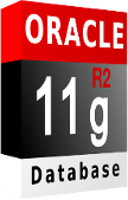
\includegraphics[scale=1]{oracle_11g}
        }
    }
    \begin{lrbox}{\litbox}
        \begin{minipage}{.949\linewidth}
            \smallskip
            }{
            \smallskip
        \end{minipage}
    \end{lrbox}
    \usebox{\litbox}
}

\newenvironment{mssql}[1][\boolean{isTable}]{
    \renewcommand*{\boolparam}{#1}
    \par
    \marginpar{
        \Ifthispageodd{
            \hspace*{0em}
        }
        {
            \hspace*{3em}
        }
        \raisebox{-3\baselineskip}{
            
\includegraphics[scale=1]{ms_sql}
        }
    }
    \begin{lrbox}{\litbox}
        \begin{minipage}{.949\linewidth}
            \smallskip
            }{
            \smallskip
        \end{minipage}
    \end{lrbox}
    \usebox{\litbox}
}

\newenvironment{msoraclesql}[1][\boolean{isTable}]{
    \renewcommand*{\boolparam}{#1}
    \par
    \marginpar{
        \Ifthispageodd{
            \hspace*{0em}
        }
        {
            \hspace*{2.8em}
        }
        \raisebox{-3\baselineskip}{
            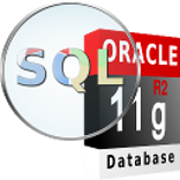
\includegraphics[scale=1]{ms_sql_oracle}
        }
    }
    \begin{lrbox}{\litbox}
        \begin{minipage}{.949\linewidth}
            \smallskip
            }{
            \smallskip
        \end{minipage}
    \end{lrbox}
    \usebox{\litbox}
}
\newenvironment{literaturinternet}{
    \par
    \vspace{.5\baselineskip}
    \marginpar{
        \Ifthispageodd{
            \hspace*{0em}
        }
        {
            \hspace*{2.8em}
        }
        \raisebox{-2\baselineskip}{
            
\includegraphics[scale=1]{globus}
        }
    }
    \begin{lrbox}{\litbox}
        \begin{minipage}{.949\linewidth}
            \smallskip
            \begin{small}
                \begin{itemize}
                    }{
                \end{itemize}
            \end{small}
            \smallskip
        \end{minipage}
    \end{lrbox}
    \fbox{\usebox{\litbox}}
    \par
    \vspace{.5\baselineskip}
    \ignorespacesafterend
}

% \newenvironment{literaturinternet}{
%   \par
%   \leaders\vbox to 2\baselineskip{%

%   }\vskip2\baselineskip
%   \marginpar{\vspace*{-1.5em}\Ifthispageodd{\hspace*{1em}}{\hspace*{3em}}
\includegraphics[scale=1]{globus}}
%   \vspace{-1.5em}
%   \begin{lrbox}{\litbox}
%     \begin{minipage}{.96\linewidth}
%       \begin{small}
%         \begin{itemize}
% }{
%         \end{itemize}
%       \end{small}
%     \end{minipage}
%   \end{lrbox}
%   \fbox{\usebox{\litbox}}
%   \par
%   \addvspace{\baselineskip}
% }

\newcommand{\bild}[3]{
    \begingroup
    \par
    \setcapindent*{-0em}
    \setcapwidth[o]{0.15\linewidth}
    \settoheight{\bildhoehe}{\includegraphics[scale=#3]{#2}}
    \addtolength{\bildhoehe}{-3em}
    \addvspace{\baselineskip}
    \begin{figure}[h!t]
        \begin{captionbeside}{#1}[o][\linewidth][4.3em]*
            \parbox[t][\bildhoehe][b]{0.85\linewidth}{
                \centering\includegraphics[scale=#3]{#2}}
        \end{captionbeside}
        \label{#2}
    \end{figure}
    \par
    \endgroup
}

\newcommand{\identifier}[1]{\textsc{#1}}
\newcommand{\languageorasql}[1]{\lstinline[language=oracle_sql]{#1}}
\newcommand{\languagemssql}[1]{\lstinline[language=ms_sql]{#1}}
\newcommand{\languagerman}[1]{\lstinline[language=rman]{#1}}
\newcommand{\languageplsql}[1]{\lstinline[language=plsql]{#1}}
\newcommand{\languagesqlplus}[1]{\lstinline[language=sqlplus]{#1}}
\newcommand{\languageconfigfile}[1]{\lstinline[language=configfile]{#1}}
\newcommand{\languageexpdpimpdp}[1]{\lstinline[language=expdp_impdp]{#1}}
\newcommand{\languagepowershell}[1]{\lstinline[language=powershell]{#1}}
\newcommand{\oscommand}[1]{\texttt{#1}}
\newcommand{\privileg}[1]{\texttt{#1}}
\newcommand{\parameter}[1]{\MakeLowercase{\textsf{#1}}}

\newcommand{\SELECT}{\languageorasql{SELECT}}
\newcommand{\FROM}{\languageorasql{FROM}}
\newcommand{\WHERE}{\languageorasql{WHERE}}
\newcommand{\GROUPBY}{\languageorasql{GROUP BY}}
\newcommand{\HAVING}{\languageorasql{HAVING}}
\newcommand{\ORDERBY}{\languageorasql{ORDER BY}}
\newcommand{\CHECK}{\languageorasql{CHECK}}
\newcommand{\NOTNULL}{\languageorasql{NOT NULL}}
\newcommand{\UNIQUE}{\languageorasql{UNIQUE}}
\newcommand{\PRIMARYKEY}{\languageorasql{PRIMARY KEY}}
\newcommand{\FOREIGNKEY}{\languageorasql{FOREIGN KEY}}
\newcommand{\INSERT}{\languageorasql{INSERT}}
\newcommand{\UPDATE}{\languageorasql{UPDATE}}
\newcommand{\DELETE}{\languageorasql{DELETE}}
\newcommand{\COMMIT}{\languageorasql{COMMIT}}
\newcommand{\ROLLBACK}{\languageorasql{ROLLBACK}}
\newcommand{\GRANT}{\languageorasql{GRANT}}
\newcommand{\REVOKE}{\languageorasql{REVOKE}}
\newcommand{\DENY}{\languageorasql{DENY}}

\newenvironment{literaturbuch}{
    \marginpar{\vspace{1em}\Ifthispageodd{\hspace*{-4em}}{\hspace*{3em}}\includegraphics[scale=1]{buch}}
    \begin{lrbox}{\litbox}
        \begin{minipage}{.975\linewidth}
            \begin{small}
                \begin{itemize}
                    }{
                \end{itemize}
            \end{small}
        \end{minipage}
    \end{lrbox}
    \par\fbox{\usebox{\litbox}}\par
}

\newcommand{\pk}[1]{\underline{#1}}
\newcommand{\fk}[1]{$\Uparrow$#1$\Uparrow$}
\newcommand{\nn}[1]{#1 [NN]}
\newcommand{\un}[1]{#1 [UN]}

\newcommand{\changefont}[3]{\fontfamily{#1} \fontseries{#2} \fontshape{#3} \selectfont}
\newcommand{\beispiel}[1]{\hyperref[#1]{Beispiel~\ref*{#1}}}
\newcommand{\abschnitt}[1]{\hyperref[#1]{Abschnitt~\ref*{#1}}}
\newcommand{\tabelle}[1]{\hyperref[#1]{Tabelle~\ref*{#1}}}
\newcommand{\abbildung}[1]{\hyperref[#1]{Abbildung~\ref*{#1}}}
\makeatletter
\newcommand{\myhref}[2]{\hyper@linkurl{#2}{#1}}
\makeatother



% KOMAScript guide, p. 66 (3.7 Dokumenttitel)
% Define title and author of this document
\title{Datenbankadministration}
\author{Florian Weidinger}

% KOMAScript guide, p. 271 ff.
\lehead*{}
\rohead*{}
\chead{\leftmark}
\makeatletter
\lofoot*{\normalfont\textbf{\@title{} \@subtitle}}
\makeatother
\rofoot*{\Large\pagemark}
\lefoot*{\Large\pagemark}

% KOMAScript guide, p. 66 (3.7 Dokumenttitel)
% Define all neccessary attributes of the title page
    \subtitle{Oracle 11g}
    \date{1. Ausgabe: 09.05.2007\linebreak Letzte Änderung: \today{}}

%%%%%%%%%%%%%%%%%%%%%%%%%%%%%%%%%%%%%%%%%%%%%%%%%%%%%%%%%%%%%%%%%%%%%%%%%%%%%%%
% Biblatex definitionen
\addbibresource{../bibliographie/bibliography.bib}

\defbibheading{oraadminguide}{\section*{Oracle Database Administrator's Guide 11g Release 2}}
\defbibheading{oraadvdevguid}{\section*{Oracle Database Advanced Application Developer's Guide 11g Release 2}}
\defbibheading{brusersguide}{\section*{Database Backup and Recovery User's Guide 11g Release 2}}
\defbibheading{oradbconcepts}{\section*{Oracle Database Concepts 11g Release 2}}
\defbibheading{oradbref}{\section*{Oracle Database Reference 11g Release 2}}
\defbibheading{oraglobsupguide}{\section*{Oracle Database Globalization Support Guide 11g Release 2}}
\defbibheading{oradbinstallguidelinux}{\section*{Database Installation Guide 11g Release 2 for Linux}}
\defbibheading{oradbinstallguidewin}{\section*{Database Installation Guide 11g Release 2 for Microsoft Windows}}
\defbibheading{oranetadmin}{\section*{Oracle Database Net Services Reference 11g Release 2}}
\defbibheading{oranetref}{\section*{Oracle Database Net Services Administrator's Guide 11g Release 2}}
\defbibheading{oraplsqlpackref}{\section*{Oracle Database PL/SQL Packages and Types Reference 11g Release 2}}
\defbibheading{orarelnoteswin}{\section*{Oracle Database Release Notes 11g Release 2 for Microsoft Windows}}
\defbibheading{orarelnoteslinux}{\section*{Oracle Database Release Notes 11g
Release 2 for Linux}} 
\defbibheading{orasecguid}{\section*{Oracle Database Security Guide 11g Release 2}}
\defbibheading{orasqlref}{\section*{Oracle Database SQL Language Reference 11g Release 2}}
\defbibheading{orautilities}{\section*{Oracle Database Utilities 11g Release 2}}
\defbibheading{others}{\section*{Andere Quellen}}
%%%%%%%%%%%%%%%%%%%%%%%%%%%%%%%%%%%%%%%%%%%%%%%%%%%%%%%%%%%%%%%%%%%%%%%%%%%%%%%

\begin{document} 
    \frontmatter
    % Typeset the title page with single line spacing
    \begin{singlespace}
        \maketitle
        \pagenumbering{Roman}
        \tableofcontents
        \pagenumbering{bychapter}
    \end{singlespace}
    \mainmatter
    
    \part{Grundlagen des Datenbankdesigns}
  \chapter{Entwicklung eines Datenmodells}
\chaptertoc{}
\cleardoubleevenpage

    In diesem Abschnitt erfolgt die Vermittlung der Kenntnisse darüber, wie man aus einer großen Menge von Informationen und Anforderungen an eine neue Datenbank eine Datenstruktur entwirft. Im Zuge der Datenmodellierung soll ein exaktes und vollständiges Modell des betrachteten Realitätsausschnitts erarbeitet werden, welches den Rahmen für die Entwicklung neuer oder die Erweiterung bestehender Anwendungssysteme bildet.

    Als Werkzeug für die Erstellung konzeptioneller Datenmodelle wird die Entity-Relation\-ship Modellierung (ER-Modellierung), zuerst in ihrer einfachsten Art und später in einer erweiterten Fassung, verwendet. Es werden dabei alle vier Phasen des Datenmodellierungsprozesses anhand eines durchgängigen Beispiels beschrieben.

    Die ER-Modellierung stellt eine spezielle \enquote{Information-Engineering-Technik} dar, die zur Erstellung von Datenmodellen hoher Qualität benutzt wird. Entworfen in den 70er Jahren von Peter Pin-Shan Chen wurde sie seither vielfach erweitert und verbessert.

    Ziel eines konzeptionellen Datenmodells ist es, die typmäßige Struktur der Daten in der Datenbank ohne deren Inhalt zu beschreiben. Als Beispiel aus der realen Welt wäre  die Ausstattung eines Büros mit Möbeln zu nennen. Wer später das Büro nutzt und mit welchem Inhalt die Schränke gefüllt werden, ist für die Erstellung des Modells Bedeutungslos.

    Die Entwicklung eines Datenmodells teilt sich in die folgenden vier Phasen ein:
    \begin{enumerate}
      \item Klassifizierung von Objekten
      \item Festlegung relevanter Eigenschaften
      \item Bestimmung identifizierender Eigenschaften
      \item Beschreibung sachlogischer Zusammenhänge zwischen den einzelnen Objekten
    \end{enumerate}
    \section{Die Modellierungsinformationen}
			Die Struktur der Bundeswehr soll in einem ER-Modell dargestellt werden.
			Es wird jedoch nur ein Ausschnitt aus der Realität betrachtet, um die
			Übersichtlichkeit der Datenstrukturen zu gewährleisten. Im Folgenden
			werden die dafür notwendigen Objekte festgelegt.
        \begin{enumerate}
          \item Die Bundeswehr besitzt zahlreiche Dienststellen an den unterschiedlichsten Standorten, welche sich untereinander über- oder untergeordnet sind. Jede Dienststelle besteht aus Dienstposten. Diese wiederum werden mit Soldaten besetzt. Jeder Soldat empfängt bei Einstieg in die Bundeswehr seine persönliche Ausrüstung und besitzt diese dann für die Dauer seines Dienstverhältnisses.
          \item Jeder Dienststelle der Bundeswehr ist eine Dienststellennummer zugeordnet, über die diese identifiziert werden kann. Des Weiteren hat jede Dienststelle eine bestimmte Größe sowie Bezeichnung, wie z. B. Führungsunterstützungsschule der Bundeswehr.
          \item Für die Standorte, an denen sich die Dienststellen befinden, müssen in der Datenbank Postleitzahl (PLZ), Ort, Straße und die Hausnummer hinterlegt sein. Hierbei ist zu beachten, dass sich eine Dienststelle auch an mehreren Standorten befinden kann.
          \item Die den Dienststellen untergeordneten Dienstposten werden durch ihre Dienstposten\_ID und ein Beginn- und Enddatum charakterisiert. Als eine weitere Eigenschaft soll eine kurze Dienstpostenbeschreibung hinterlegt werden.
          \item Jeder in der Datenbank aufgeführte Soldat soll dort mit seiner Personanlnummer, einer Personenkennziffer, sowie Vor- und Nachnamen und Dienstgrad aufgeführt werden. Weiterhin kann der Anwender auch die aktuelle Adresse, bestehend aus PLZ, Wohnort, Straße und Hausnummer, aus der Datenbank heraussuchen.
          \item Das letzte Objekt in der Datenbank stellt die persönliche Ausrüstung des Soldaten dar. Diese besitzt eine Bezeichnung, ist aus einem bestimmten Material gefertigt und hat eine Farbe. Für eine bessere Zuordnung ist jeder Aurüstungsgegenstand mit einer Versorgungsnummer versehen.
        \end{enumerate}
    \section{Klassifizierung von Objekten}
      Das im vorigen Abschnitt vorgestellte Beispiel stellt nur einen kleinen Ausschnitt aus der Realität dar. Komplexer gestaltete Datenbanken können aus weit mehr Objekten bestehen.
      Um dabei nicht den Überblick über diese Flut von Objekten zu verlieren, werden diese in Klassen gruppiert. Diese Objektklassen enthalten dann die Objekte, die von ihrer Art her gleich sind und über die die gleichen Informationen gesammelt werden. Damit wird eine Abstraktionsebene gebildet, die es ermöglicht, von den Besonderheiten der einzelnen Objekte abzusehen und nur das typische der gebildeten Objektklassen zu berücksichtigen.
      \subsection{Definitionen und Syntaxregeln}
				Für die Darstellung der Objekttypen gelten folgende syntaktische
				Regeln:
				\begin {enumerate}
					\item Ein Objekttyp wird durch ein Rechteck dargestellt, in dessen
					Mitte der Objekttypname eingetragen wird.
					\begin{center}
						\scalebox{1}{
							\begin{tikzpicture}[node distance=1.5cm, every edge/.style={link}]
								\node[entity](e1){Soldat};
							\end{tikzpicture}
						}
					\end{center}
					\item Die Größe und Position des Rechtecks sind bedeutungslos.
					\item Der Objekttypname steht im Singular und muss für
					das gesamte Datenmodell eindeutig sein.
        \end{enumerate}
        \begin{merke}
            \begin{itemize}
                \item \textbf{Objekt}: Ein Objekt (engl. Entity) ist ein Exemplar von Personen, Gegenständen oder nichtmateriellen Dingen, über das Informationen gespeichert wird, z. B. der konkrete Soldat Max Mustermann.
                \item \textbf{Objekttyp}: Ein Objekttyp (engl. Entity type) ist eine durch einen Objekttyp-namen eindeutig benannte Klasse von Objekten, über die dieselben Informationen gespeichert und die prinzipiell in gleicher Weise verarbeitet werden, wie z. B. die benannte Klasse bzw. der Objekttyp SOLDAT.
            \end{itemize}
        \end{merke}

        Die Bildung von Objekttypen hängt entscheidend von den Anforderungen
        des jeweils zu modellierenden Gegenstandsbereiches ab. Aus der Sicht
        eines Großhändlers kann ein Unternehmen mit all seinen Bereichen
        als ein einziger Objekttyp gesehen werden. Dasselbe Unternehmen dagegen
        wird aus seiner eigenen Sicht detailliert mit seinen Bereichen,
        Abteilungen, Mitarbeitern, Werkshallen, Fahrzeugen usw. zu modellieren
        sein. Diese Modellierung ist ebenfalls nicht eine einmalige, in sich
        abgeschlossene Tätigkeit, denn im Laufe der Zeit müssen Änderungen
        der Realität auch im Modell eingearbeitet werden.
      \subsection{Traditionelles Pendant}
        Die Informationsverarbeitung mit Hilfe elektronischer Datenverarbeitung
        hat hinsichtlich der Datenspeicherung nur wenig prinzipiell neue
        Methoden entwickelt. Fast alle Konzepte, in Bezug auf das
        Entity-Relationship-Modell, haben ihr Pendant in der traditionellen
        Informationsspeicherung. Zum besseren Verständnis der eingeführten
        Begriffe wird auf diese Zusammenhänge an den entsprechenden Stellen
        hingewiesen.

        So entsprechen die Objekttypen den traditionellen Karteikästen und die
        Objekte eines Objekttyps den Karteikarten, die in einem Karteikasten
        eingeordnet sind. In der traditionellen Arbeitsweise würde für
        \enquote{Axel Schweiss} eine Karteikarte angelegt werden und z. B. im
        Karteikasten \enquote{Soldat} abgelegt werden
\clearpage
    \section{Festlegung der relevanten Eigenschaften}
      Im ersten Schritt, der Klassifizierung von Objekten, wurden Objekte, die
      in gleicher Art und Weise verarbeitet werden, in Objekttypen
      zusammengefasst. Um die Verarbeitung dieser Objekte automatisiert
      durchführen zu können, ist es Voraussetzung, dass jeder Objekttyp
      bestimmte Angaben speichert. Diese Angaben werden für die elektronische
      Verarbeitung entweder als Eingabeinformation oder als Ausgabeinformation
      benötigt.
      
      Aus diesem Grund ist es notwendig, für jeden Objekttyp die relevanten
      Eigenschaften der Objekte, die in ihm zusammengefasst werden, anzugeben.
      Damit wird der durch den Objekttyp definierte Begriff auf einen Satz
      relevanter Eigenschaften reduziert. Die Festlegung dieser Eigenschaften
      ist aber nur bei genauer Kenntnis der Geschäfts- und
      Verarbeitungsprozesse des Auftraggebers möglich. Ohne diese Kenntnisse
      befindet man sich in jedem Falle im Bereich von Spekulationen.
      \subsection{Definitionen und Syntaxregeln}
        \begin{merke}
          \begin{itemize}
            \item \textbf{Eigenschaft:} Eine Eigenschaft (engl. Attribute) ist
            die Benennung für ein relevantes Merkmal aller Objekte, die in
            einem Objekttyp zusammengefaßt werden, z. B. Soldaten haben die
            Eigenschaft Dienstgrad.
            \item \textbf{Eigenschaftswert:} Ein Eigenschaftswert (engl.
            Attribute value) ist eine spezielle Ausprägung, die eine
            Eigenschaft für ein konkretes Objekt annimmt, z. B. der Dienstgrad
            Hauptfeldwebel.
          \end{itemize}
          \end{merke}

        Für die Darstellung der Eigenschaften gelten folgende Regeln:
        \begin {enumerate}
          \item Die Benennung der Eigenschaft wird als Blase an den Objekttyp
          angehängt.

          \begin{center}
           \scalebox{1}{
            \begin{tikzpicture}[node distance=1.5cm, every edge/.style={link}]
              \node[entity](e1){Soldat};
                \node[attribute](a1)[right = of e1]{Dienstgrad} edge (e1);
            \end{tikzpicture}
           }
          \end{center}
          \item Die Reihenfolge der Eigenschaften ist bedeutungslos.
          \item Die Benennung der Eigenschaft steht im Singular und muss für
          den Objekttyp eindeutig sein.
        \end{enumerate}
        Auch an dieser Stelle wird eine Abstraktion der realen Welt
        vorgenommen, in dem statt der Eigenschaftswerte, die jedes einzelne
        Objekt besitzt, nur die Eigenschaften der Objekttypen angegeben werden.
        Um diesen Abstraktionsprozess korrekt durchführen zu können, bedarf
        es der Einhaltung einiger Regeln:
        \begin{itemize}
          \item Es darf niemals ein Eigenschaftswert als Eigenschaftsname
					verwendet werden (beispielsweise anstatt 02.05.1985 die Bezeichnung
					\enquote{Geburtsdatum} oder statt \enquote{männlich} die Bezeichnung
					\enquote{Geschlecht}).
          \item Die Bezeichnung eines Objekttyps sollte niemals im
					Eigenschaftsnamen auftauchen, da dieser immer nur im Kontext
					des Objekttyps gilt (z. B. Person mit der Eigenschaft Name, nicht
					\enquote{Personname}, sondern die Eigenschaft \enquote{Name}
					wählen).
          \item Bei komplexen Eigenschaften wie z. B. einer Adresse oder einer
					PK stellt sich immer wieder die Frage, ob diese zerlegt werden
					müssen oder ob sie als atomar \footnote{atomare Information = eine
					einzige, nicht mehr teilbare Information} betrachtet werden. Die
					Antwort auf diese Frage ist abhängig von den einzelnen
					Verarbeitungsprozessen, denen diese Daten unterliegen. Muss
					beispielsweise die Information verfügbar sein, von welchem
					Kreiswehrersatzamt ein Soldat betreut wird, so muss  die PK in ihre
					Bestandteile zerlegt werden. Ist diese Information irrelevant, kann
					die PK im ganzen als atomar betrachtet werden.
          \item Problematisch ist auch die Entscheidung, ob speicherwürdige
          Informationen als Eigenschaften oder als ein eigenständiger
          Objekttyp betrachtet werden sollen. Um einen eigenständigen
          Objekttyp handelt es sich immer dann, wenn er für das Unternehmen
          bedeutsame Objekte enthält, die relevante individuelle Eigenschaften
          besitzen.
        \end{itemize}
      \subsection{Traditionelle Datenspeicherung}
        Die Eigenschaften eines Objekttyps A entsprechen den Feldern, die auf
        einer Karteikarte zur Aufnahme der relevanten Informationen angelegt
        werden. Durch die gewählten Eigenschaften wird also die einheitliche
        Struktur aller Karteikarten eines Kastens festgelegt.

        Welche Eigenschaften können Sie, bezogen auf das Beispiel
        \enquote{Bundeswehr}, den identifizierten Objekttypen zuordnen?
        \subsubsection{Lösungsvorschlag}
          \begin{itemize}
            \item Objekttyp \enquote{Dienststelle}: Dienststellennummer,
            Bezeichung
            \item Objekttyp \enquote{Standort}: PLZ, Ort, Straße, Hausnummer
            \item Objekttyp \enquote{Dienstposten}: Dienstposten\_ID,
            Beginndatum, Enddatum, Dienstpostenbeschreibung
            \item Objekttyp \enquote{Soldat}: Personalnummer, PK, Name, Vorname,
            Dienstgrad, PLZ, Ort, Straße, Hausnummer
            \item Objekttyp \enquote{Ausrüstung}: Versorgungsnummer, Material,
            Farbe
          \end{itemize}
    \section{Festlegung der Identifizierung}
      Ein Objekttyp stellt die Zusammenfassung mehrerer gleichartiger Objekte
      dar. Gleichartig bedeutet, dass diese Objekte die gleichen Eigenschaften
      aufweisen und die Verarbeitungsprozesse für all diese Objekte gleich
      sind. Die einzelnen Objekte eines Objekttyps müssen aber voneinander
      unterscheidbar sein. Deshalb muss festgelegt werden, auf welche Weise ein
      Objekt innerhalb des Objekktyps identifiziert werden kann.

      \subsection{Identifizierungsvarianten}
        Für die Identifizierung eines Objekts innerhalb eines Objekttyps
        stehen die konkreten Eigenschaftswerte des Objekts zur Verfügung.

        Es werden drei Varianten zur Identifizierung von Objekten
        unterschieden.
        \subsubsection{Identifizierung eines Objekts durch eine einzelne
Eigenschaft}
          Es kann vorkommen, dass die Eigenschaftswerte einer Eigenschaft eines
          Objekttyps eindeutig ist. D. h. jeder Eigenschaftswert dieser
          Eigenschaft ist so geartet, dass jedes Objekt dieses Objekttyps einen
          unterschiedlichen Wert für diese Eigenschaft hat. Durch Angabe
          dieses Eigenschaftswertes ist dann das Objekt eindeutig identifiziert.

          Beispiel: Soldaten werden i. d. R. durch ihre PK eindeutig
          identifiziert

				\subsubsection{Identifizierung eines Objekts durch eine Kombination
mehrerer Eigenschaften}
          In einigen Fällen ist keine der Eigenschaften eines Objekttyps
          geeignet, alleine als identifizierende Eigenschaft zu fungieren. Um
          dieses Problem zu lösen kann versucht werden, eine
          \underline{minimale} Kombination von Eigenschaften eines Objekttyps
          als Identifikationsmerkmal zu benutzen. Dies funktioniert dann, wenn
          die Kombination der Werte der entsprechenden Eigenschaften bei jedem
          Objekt eindeutig sind.

          Beispiel: Die Kombination der beiden Attribute PLZ und Ortsbezeichnung ist eindeutig,
					eine Eigenschaft alleine nicht.

				\subsubsection{Identifizierung eines Objekts durch eine organisatorische
Eigenschaft}
          Sollte es dennoch vorkommen, dass weder eine einzelne Eigenschaft, noch eine
					Kombination von Eigenschaften zur Identifikation der Objekte eines
					Objekttyps geeignet ist, kann eine künstliche Eigenschaft
					eingeführt werden, bei der die Eindeutigkeit durch organisatorische
					Maßnahmen gewährleistet wird.

					Ein Beispiel hierfür wäre eine Ort\_ID, die es möglich
					macht, einen Ort eindeutig zu bestimmen ohne die Kombination aus PLZ
					und Ortsnamen heranziehen zu müssen.

          Es ist aber auch möglich, dass eine organisatorische Eigenschaft
          gewählt wird, da abzusehen ist, dass eine identifizierende
          Eigenschaft durch eine andere ersetzt werden soll. Die
          Umstrukturierung der Datenbank wäre zu aufwendig und zu komplex.

          Ein Beispiel aus der Praxis ist die PK und die Personalnummer eines
          jeden Soldaten. Die Personalnummer wird in geraumer Zeit die PK
          ersetzen. Es ist aus diesem Grund von Vorteil eine organisatorische
          Eigenschaft, wie die Personen\_ID zu wählen, um eine
          Umstrukturierung zu vermeiden.

          Weitere Beispiele für organisatorische Eigenschaften sind die beiden Attribute Artikelnummer und LfdNr.

          Die Identifizierung der Objekte eines Objekttyps mittels einer
					\enquote{organisatorischen Eigenschaft} ist bei der automatisierten
					Datenverarbeitung eine beliebte Vorgehensweise. Sie wird häufig
					selbst dann angewendet, wenn natürliche identifizierende
					Eigenschaften vorhanden sind. Meist handelt es sich um eine laufende
					Nummer.

					Dies hat den Vorteil, dass kurze identifizierende Eigenschaftswerte
					entstehen. Der Nachteil ist, dass Werte wie z. B. eine laufende
					Nummer meist keinerlei Aussagekraft haben und somit Gefahren wie
					Verwechslung oder Fehleingabe entstehen.

					Die Festlegung der Identifizierungsform für einen Objekttyp muss mit
					großer Sorgfalt erfolgen. Relationale Datenbank-Managementsysteme
					für die wir unsere Modellierung durch\-füh\-ren, lassen es
					nämlich nicht zu, dass zwei Objekte desselben Objekttyps in der
					Kombination ihrer identifizierenden Merkmale übereinstimmen. Bleibt
					ein Restrisiko hinsichtlich der Unikalität der identifizierenden
					Merkmale und treten dann bei der praktischen Datenbankarbeit
					tatsächlich zwei Objekte mit übereinstimmenden Werten ihrer
					identifizierenden Merkmale auf, lehnt das Datenbank-Managementsystem
					die Speicherung des zweiten Objekts ab.

					\begin{merke}
						Um ein Modell übersichtlich und verständlich zu halten, sollte
						konsequent immer nur eine der drei zur Verfügung stehenden
						Methoden für die Identifizierung von Objekten genutzt werden!
          \end{merke}
          
			\subsection{Markierung der Identifizierenden Eigenschaft}
				Für die Markierung der (teil)identifizierenden Eigenschaft gelten
				die folgenden syntaktischen Regeln (diese werden u. U. in Kombination
				mit anderen angewendet):
        \begin {enumerate}
          \item Eine identifizierende Eigenschaft (bzw. jede teilidentifizierende Eigenschaft) wird durch Unterstreichung kenntlich gemacht.

          \begin{center}
           \scalebox{1}{
            \begin{tikzpicture}[node distance=1.5cm, every edge/.style={link}]
              \node[entity](e1){Soldat};
							\node[attribute](a1)[right = of e1]{\key{Personalnummer}} edge
(e1);
            \end{tikzpicture}
           }
          \end{center}
          \item Die Position der (teil)identifizierenden Eigenschaft innerhalb der Liste der Eigenschaften ist bedeutungslos. Sie sollte jedoch aus Gründen der Übersichtlichkeit immer zu erst genannt werden.
        \end{enumerate}
      \subsection{Klassisches Pendant}
        Bei der traditionellen Informationsspeicherung mit Hilfe von Karteikästen entspricht der Identifizierung die Festlegung eines Kennbegriffs: Üblicherweise wird im Kopf einer Karteikarte für das betreffende Objekt ein Wert angegeben, der das Objekt innerhalb des Karteikastens identifiziert\footnote{Kennbegriff wird oft auch als \enquote{Reiter} bezeichnet}. Um eine bestimmt Karteikarte manuell schneller finden zu können, werden die Karteikarten des Karteikastens nach diesem Begriff sortiert.

        Betrachten wir wieder das Beispiel \enquote{Bundeswehr}. Welche Objekteigenschaften kön\-nen Ihrer Meinung nach als identifizierende Merkmale verwendet werden?
        \subsubsection{Lösungsvorschlag}
          \begin{itemize}
            \item Objekttyp \enquote{Dienststelle}: Dienststellennummer
            \item Objekttyp \enquote{Standort}: PLZ, Ort
            \item Objekttyp \enquote{Dienstposten}: Dienstposten\_ID
            \item Objekttyp \enquote{Soldat}: Personalnummer
            \item Objekttyp \enquote{Ausrüstung}: Versorgungsnummer
          \end{itemize}
          An dieser Stelle wird die Entscheidung getroffen, dass für die Fortführung dieses Modells organisatorische Einheiten als identifizierende Eigenschaften eingeführt werden!
          \begin{itemize}
            \item Objekttyp \enquote{Dienststelle}: Dienststellen\_ID
            \item Objekttyp \enquote{Standort}: Ort\_ID
            \item Objekttyp \enquote{Dienstposten}: DP\_ID
            \item Objekttyp \enquote{Soldat}: Personen\_ID
            \item Objekttyp \enquote{Ausrüstung}: Ausruestungs\_ID
          \end{itemize}

    \section{Modellierungsformen}
          \begin{center}
           \scalebox{.6}{
            \begin{tikzpicture}[node distance=1.5cm, every edge/.style={link}]
              \node[entity](dienstposten){Dienstposten};
                \node[attribute](dpid)[above = of dienstposten]{\key{DP\_ID}} edge (dienstposten);
                \node[attribute](dienstpostenid)[above left = of dienstposten]{Dienstposten\_ID} edge (dienstposten);
                \node[attribute](begindatum)[above right = of dienstposten]{Beginndatum} edge (dienstposten);
                \node[attribute](enddatum)[below right = of dienstposten]{Enddatum} edge (dienstposten);
                \node[attribute](dienstpostenbeschreibung)[below left = of dienstposten]{Dienstpostenbeschreibung} edge (dienstposten);
              \node[entity](soldat)[below left = 6cm of dienstposten]{Soldat};
                \node[attribute](personenid)[above = 1.6cm of soldat]{\key{Personen\_ID}} edge (soldat);
                \node[attribute](pk)[above right = of soldat]{PK} edge (soldat);
                \node[attribute](name)[below right = of soldat]{Name} edge (soldat);
                \node[attribute](vorname)[below left = of soldat]{Vorname} edge (soldat);
                \node[attribute](dienstgrad)[above left = of soldat]{Dienstgrad} edge (soldat);
              \node[entity](ausruestung)[below = 6cm of soldat]{Ausrüstung};
                \node[attribute](versorgungsnummer)[above left = of ausruestung]{Versorgungsnummer} edge (ausruestung);
                \node[attribute](bezeichnung)[above = 1.7cm of ausruestung]{Bezeichnung} edge (ausruestung);
                \node[attribute](ausruestungsid)[above right = of ausruestung]{\key{Ausruestungs\_ID}} edge (ausruestung);
                \node[attribute](material)[below right = of ausruestung]{Material} edge (ausruestung);
                \node[attribute](farbe)[below left = of ausruestung]{Farbe} edge (ausruestung);
              \node[entity](dienststelle)[below right = 6cm of dienstposten]{Dienststelle};
                \node[attribute](dienststellennummer)[below left = of dienststelle]{\key{Dienststellen\_ID}} edge (dienststelle);
                \node[attribute](dienststellennummer)[above left = of dienststelle]{Dienststellennummer} edge (dienststelle);
                \node[attribute](bezeichung)[above right = of dienststelle]{Bezeichnung} edge (dienststelle);
                \node[attribute](groesse)[below right = of dienststelle]{Größe} edge (dienststelle);
              \node[entity](standort)[below = 6cm of dienststelle]{Standort};
                \node[attribute](ortid)[above = of standort]{\key{Ort\_ID}} edge (standort);
                \node[attribute](plz)[above left = of standort]{PLZ} edge (standort);
                \node[attribute](ort)[above right = of standort]{Ort} edge (standort);
                \node[attribute](strasse)[below right = of standort]{Straße} edge (standort);
                \node[attribute](hausnummer)[below left = of standort]{Hausnummer} edge (standort);
            \end{tikzpicture}
           }
          \end{center}
        Hinweis: Das Objekt Soldat enthält nicht alle Attribute. Es fehlen die Attribute Personalnummer, Plz, Ort, Straße und Hausnummer.

  \chapter{Beschreibung sachlogischer Zusammenhänge zwischen Objekttypen}
  \chaptertoc{}
  \cleardoubleevenpage
  
  Bisher wurden im Rahmen der Datenmodellierung die speicherwürdigen Objekte mit ihren relevanten Eigenschaften lediglich isoliert beschrieben. In der Praxis stehen die interessanten Objekte jedoch in vielfältiger Weise miteinander in Zusammenhang: Dienststellen befinden sich an Orten, Soldaten arbeiten in Dienststellen usw. Auch Objekte desselben Typs können miteinander in Zusammenhang stehen: Lehrer leiten Lehrer an, Schulen haben Partnerschaften mit anderen Schulen usw. Diese Zusammenhänge müssen ebenfalls im Datenmodell dargestellt werden, denn sie bringen wesentliche Aspekte der betrachteten Realität zum Ausdruck.

    Die sachlogischen Zusammenhänge zwischen den Objekten werden in drei Gruppen von Beziehungstypen unterteilt:
    \begin{itemize}
      \item \textbf{Binäre Beziehungstypen}: Beschreiben den Zusammenhang zwischen jeweils zwei Objekten, die verschiedenen Objekttypen angehören.
      \item \textbf{Beziehungstypen n-ten Grades}: Sie Beschreiben den Zusammenhang zwischen mehr als zwei Objekten, die verschiedenen Objekttypen angehören.
      \item \textbf{Rekursiv-Beziehungstypen}: Objekte, die aus demselben Objekttyp stammen, stehen in Zusammenhang.
    \end{itemize}

    Im Folgenden werden nur die binären oder auch dualen Beziehungstypen erläutert. Auf Beziehungstypen höheren Grades wird im
    weiteren Verlauf nicht eingegangen, da diese in der Praxis kaum Relevanz besitzen. Die Behandlung der Rekursiven
    Beziehungstypen erfolgt im Kapitel 3.

      Für den weiteren Verlauf sind die nachfolgenden zwei Definitionen zu unterscheiden:
      \begin{itemize}
        \item \textbf{Beziehung (engl. Relationship)}: Kennzeichnet den konkreten Zusammenhang zwischen zwei realen Objekten. Beispiel: \enquote{Max Mustermann} ist Lehrgangsteilnehmer im Lehrgang \enquote{Datenbank Administrator}
        \item \textbf{Beziehungstypen}: Beschreibt den typmäß igen Zusammenhang, der zwischen den Objekttypen besteht. Beispiel: Objekttypen sind \enquote{Soldat} \enquote{Lehrgang} mit dem Beziehungstyp \enquote{ist Lehrgangsteilnehmer in}
      \end{itemize}

      Während in der realen Welt der Zusammenhang zwischen zwei konkreten Objekten \textbf{beobachtet} wird, \textbf{beschreibt} man in der Modellwelt das verallgemeinerte Wechselspiel zwischen zwei Objekttypen. Im mathematischen Sinne ist ein Beziehungstyp zwischen den Objekten A und B die Menge der Beziehungen zwischen jeweils einem Objekt aus dem Objekttyp A und einem Objekt aus dem Objekttyp B. Die für den Beziehungstyp formulierten Angaben müssen somit für alle konkreten Beziehungen zwischen den betrachteten Objekttypen gültig sein.
      \section{Benennung, Optionalität und Kardinalität}\label{naming_optionaliy_kardinality}
        Der sachlogische Zusammenhang zwischen den Objekten zweier Objekttypen, der durch einen Beziehungstyp beschrieben wird, besteht immer in \textbf{beiden Richtungen}: Soldaten stehen beispielsweise in einem Zusammenhang mit Dienststellen (sie arbeiten dort) und Dienststellen stehen im Zusammenhang mit Soldaten (sie beschäftigen sie). Jede der beiden Beziehungstyp-Richtungen wird durch 3 Angaben näher bestimmt.
        \subsection{Benennung}
          Betrachtet man im Beispiel aus Kapitel 1.1 den Zusammenhang zwischen Soldat und Ausrüstung, könnte man sich für folgende Dinge interessieren:
          \begin{itemize}
            \item Ein Soldat besitzt Ausrüstung.
            \item Ein Soldat empfängt seine Ausrüstung.
            \item Ein Soldat hat bestimmte Ausrüstungsgegenstände mitzuführen.
          \end{itemize}
          Welcher Zusammenhang gespeichert werden soll, wird durch die Benennung zum Ausdruck gebracht.
          Hier ist es \enquote{besitzt}.
        \subsection{Optionalität}
          Die Optionalität klärt die Frage, ob jedes Objekt des Objekttyps A mit mindestens einem Objekt des Objekttyp B in Beziehung stehen muss? Je nach Antwort unterscheidet man zwei Fälle:
          \begin{itemize}
            \item \textbf{Ja}: Die Beziehungstyp-Richtung wird als nichtoptional, also als \textbf{obligatorisch\footnote{obligare lat. = bindend, verpflichtend}} bezeichnet.
            \item \textbf{Nein}: Die Beziehungstyp-Richtung wird als optional, also \textbf{kann vorhanden sein} bezeichnet.
          \end{itemize}
        \subsection{Kardinalität}
          Für die Angabe der Kardinalität einer Beziehungstyp-Richtung vom Objekttyp A zum Objekttyp B stellt man sich folgende Frage: \enquote{Kann ein Objekt des Objekttyps A mit mehreren Objekten des Objekttyps B in Beziehung stehen?} Es können dabei zwei unterschiedliche Fälle auftreten:
\clearpage
          \begin{itemize}
            \item \textbf{Ja}: Der Beziehungstyp-Richtung wird die Kardinalität \textbf{N} zugeordnet. Dabei steht \textbf{N} für eine beliebige Zahl größ er oder gleich 0.
            \item \textbf{Nein}: Die Beziehungstyp-Richtung wird die Kardinalität \textbf{1} zugeordnet, denn es gibt \textbf{höchstens ein} Objekt des Objekttyps B zu dem Objekt aus Objekttyp A.
          \end{itemize}
        \subsection{Darstellung im Modell}
          Es gibt verschiedene Formen der Darstellung. Man kann jede Beziehungstyp-Richtung benennen, jedoch ist die Benennung meist nur für eine Richtung passend. Die Gegenrichtung müsste dann bei Bedarf umformuliert werden. Im Folgenden soll ein Beispiel die Zusammehänge zwischen Benennung, Optionalität und Kardinalität zeigen. Gegeben seien die Objekttypen Soldat und Ausrüstung mit der angezeigten Beziehung.

          \begin{center}
            \scalebox{.7}{
              \begin{tikzpicture}[node distance=1.5cm, every edge/.style={link}]
                \node[entity](soldat){Soldat};
                  \node[attribute](personenid)[above = 1.6cm of soldat]{\key{Personen\_ID}} edge (soldat);
                  \node[attribute](pk)[above right = of soldat]{PK} edge (soldat);
                  \node[attribute](name)[below right = of soldat]{Name} edge (soldat);
                  \node[attribute](vorname)[below left = of soldat]{Vorname} edge (soldat);
                  \node[attribute](dienstgrad)[above left = of soldat]{Dienstgrad} edge (soldat);
                \node[relationship](besitzt)[right = 3cm of soldat]{besitzt} edge node[auto,swap] {n}(soldat);
                \node[entity](ausruestung)[right = 8cm of soldat]{Ausrüstung} edge node [auto,swap] {m}(besitzt);
                  \node[attribute](ausruestungsid)[right = of ausruestung]{\key{Ausruestungs\_ID}} edge (ausruestung);
                  \node[attribute](versorgungsnummer)[below right = of ausruestung]{Versorgungsnummer} edge (ausruestung);
                  \node[attribute](bezeichnung)[above = 1.7cm of ausruestung]{Bezeichnung} edge (ausruestung);
                  \node[attribute](material)[above left = of ausruestung]{Material} edge (ausruestung);
                  \node[attribute](farbe)[below left = of ausruestung]{Farbe} edge (ausruestung);
            \end{tikzpicture}
            }
          \end{center}

        Zu diesem Ausschnitt aus einem ER-Modell ergeben sich die drei folgenden Fragen:
        \begin{enumerate}
          \item Welcher Zusammenhang soll ausgedrückt werden (\textbf{Benennung})?

          Durch die Benennung der beiden Objekttypen mit \enquote{Soldat} und \enquote{Ausrüstung} zeigt sich der Zusammenhang, dass ein Soldat Ausrüstung besitzt.
          \item Sind die beiden Objekttypen aneinader gebunden (\textbf{Optionalität})?

          In diesem Beispiel ist es so, dass ein Soldat Ausrüstung besitzen kann aber nicht muss, z.B. vor der Einkleidung ist man schon Soldat, obwohl noch jegliche Ausrüstungsgegenstände fehlen. Anders herum ist es möglich, dass Ausrüstungsgegenstände einem Soldaten
          zugeordnet wurden oder der Ausrüstungsgegenstand noch im Lager liegt.
          Antwort: Beide Richtungen sind optional.
          \item Wie stehen die beiden Objekttypen in Zusammenhang (\textbf{Kardinalität})?

          \begin{itemize}
            \item Fragerichtung vom Objekttyp \enquote{Soldat}  zum Objekttyp \enquote{Ausrüstung}:
            \enquote{Kann ein Soldat mehrere Ausrüstungsgegenstände besitzen?}, Antwort: Ja, daher N.
            \item Fragerichtung vom Objekttyp \enquote{Ausrüstung}  zu \enquote{Soldat}:

            \enquote{Kann ein Ausrüstungsgegenstand von mehreren Soldaten besessen werden?}
            Antwort: Ja, d. h. die Kardinalität lautet M.
          \end{itemize}
        \end{enumerate}
        Ein Ausrüstungsgegenstand ist durch eine Versorgungsnummer
        gekennzeichnet. Somit ist es möglich, unterschiedliche
        Ausrüstungsgegenstände mit der gleichen Versorgnugnsnummer an die
        Soldaten auszugeben. Es entsteht eine \enquote{N:M} Kardinalität (vgl.
        \ref{NotationKardinalitaet}).

        Bei der Festlegung der Kardinalität ist auß erdem zu beachten,
        über welchen Zeitraum hinweg die Angaben zu Beziehungen in der
        Datenbank aufgenommen werden sollen. Bei der Beziehung \enquote{Soldat
        arbeitet in Dienststelle}, ist die Kardinalität auf 1 zu setzen, wenn
        der Soldat immer nur in einer Dienststelle arbeiten soll. Will man aber
        die Zuordnungsverhältnisse über einen längeren Zeitraum speichern,
        so ist die Kardinalität auf N festzulegen, weil es dann vorkommen
        kann, dass ein Soldat mit mehreren Dienststellen in Verbindung gebracht
        werden muss, also eine Historie gespeichert wird.
      \section{Notationen für Kardinalitäten} \label{NotationKardinalitaet}
        Für die Kardinalität gibt es verschiedene Notationen, also
        einheitliche Schreibweisen. In dieser Unterlage wird die Chen-Notation
        kurz vorgestellt und die (Min,Max)-Notation eingehender behandelt.
        Sofern die Chen-Notation von Interesse ist, kann diese in vielen
       Fachbüchern leicht nachgelesen werden.
        \subsection{Die Chen-Notation}
          In der Chen-Notation gibt es im Wesentlichen drei verschiedene
          Beziehungstypen, dabei ist es unerheblich, ob die verwendeten
          Buchstaben groß\ oder klein geschrieben werden. Die Werte geben die
          maximale Anzahl von beteiligten Objekten an.

          Mögliche Varianten (binäre Beziehungen):
          \begin{itemize}
            \item 1:1
            \item 1:n
            \item n:m
            \item n:m:k (ternäre Beziehungen)
          \end{itemize}
          Welche Werte können angenommen werden bzw. wofür stehen die
          Buchstaben?
          \begin{itemize}
            \item n: beliebig viele (0,1,2...n)
            \item 1: höchstens ein (0 oder 1)
            \item m oder k: entsprichen der n-Definition
          \end{itemize}
          Die Angabe von genaueren Werten ist in der Chen-Notation nicht
          vorgesehen.
        \subsection{(Min,Max)-Notation}
          Die (Min,Max)-Notation ist im Wesentlichen eine Konkretisierung der
          Angaben in der Chen-Notation, denn es werden nicht nur die maximalen,
          sondern auch die minimalen Werte angegeben. Folgende Abbildung zeigt
          die oben verwendete Beziehung in der (Min,Max)-Notation.
          \begin{center}
            \scalebox{.7}{
              \begin{tikzpicture}[node distance=1.5cm, every edge/.style={link}]
                \node[entity](soldat){Soldat};
                  \node[attribute](personenid)[above = 1.6cm of soldat]{\key{Personen\_ID}} edge (soldat);
                  \node[attribute](pk)[above right = of soldat]{PK} edge (soldat);
                  \node[attribute](name)[below right = of soldat]{Name} edge (soldat);
                  \node[attribute](vorname)[below left = of soldat]{Vorname} edge (soldat);
                  \node[attribute](dienstgrad)[above left = of soldat]{Dienstgrad} edge (soldat);
                \node[relationship](besitzt)[right = 3cm of soldat]{besitzt} edge node[auto,swap] {(0,*)}(soldat);
                \node[entity](ausruestung)[right = 8cm of soldat]{Ausrüstung} edge node [auto,swap] {(0,*)}(besitzt);
                  \node[attribute](ausruestungsid)[above right = of ausruestung]{\key{Ausruestungs\_ID}} edge (ausruestung);
                  \node[attribute](versorgungsnummer)[below right = of ausruestung]{Versorgungsnummer} edge (ausruestung);
                  \node[attribute](bezeichnung)[above = 1.7cm of ausruestung]{Bezeichnung} edge (ausruestung);
                  \node[attribute](material)[above left = of ausruestung]{Material} edge (ausruestung);
                  \node[attribute](farbe)[below left = of ausruestung]{Farbe} edge (ausruestung);
            \end{tikzpicture}
            }
          \end{center}

          Welche Werte können angenommen werden bzw. wofür stehen diese Werte? Bei der Min, Max-Notation gibt es eine Vielzahl von Möglichkeiten, diese hier aufzulisten, wäre schier unmöglich. Daher einige häufige Kombinationen.

          \tablefirsthead{%
            \multicolumn{1}{l}{\textbf{Möglichkeit}} &
            \multicolumn{1}{l}{\textbf{Bedeutung}} \\
          }
          \begin{supertabular}[ht]{lp{11cm}}
            (1,1) & genau 1 $\Longrightarrow$ mindestens 1 und höchstens 1\\
            (1,*) & mindestens 1 $\Longrightarrow$ mindestens 1 und höchstens beliebig viele\\
            (0,1) & höchstens 1 $\Longrightarrow$ mindestens 0 und höchstens 1\\
            (0,*) & kann haben $\Longrightarrow$ 0 oder beliebig viele\\
            \\
            (2,100) & mindestens 2 und höchstens 100\\
            (4,*) & mindestens 4 und höchstens beliebig viele\\
          \end{supertabular}

          Die beiden letzten Zeilen der obigen Auflistung sollen verdeutlichen, dass für die Min- und Max-Werte beliebige ganze Zahlen verwendet werden können. Hier ist jedoch zu beachten, dass die Umsetzung bestimmter Kombinationen in den Kardinalitäten in einem relationalen Datenbanksystem nicht mehr mit der referentiellen Integrität sichergestellt werden kann, sondern mit Elementen einer Programmiersprache auf Seiten der Anwendung oder der Datenbank. Später dazu mehr.
          \subsection{Schreib-/Leseweise der Kardinalitäten}
          Für die Syntax der Kardinalitäten gilt folgende Vorgehensweise.
          \begin{itemize}
            \item Die (Min,Max)-Notation: Man betrachtet zunächst ein Objekt a auf der Seite des Objekttyps A und schreibt die Kardinalität auf die gleiche Seite des Beziehungstyps, an den Objekttyp A.
            \item (Chen)-Notation: Inverse Bezeichnung der Kardinalitäten wie bei der (Min,Max)-Notation. Die Kardinalität des Objekts a auf der Seite des Objekttyps A wird auf die andere Seite des Beziehungstyps, also Objekttyp B, geschrieben.
            \item Anschließ end in gleicher Weise am Objekttyp B für die jeweilige Notation.
          \end{itemize}
          \subsection{Referentielle Integrität}
            Die Referentielle Integrität stellt einen Satz aus zwei Regeln dar, der dazu dient, den korrekten Zusammenhang zwischen den Datensätzen zweier Tabellen zu regeln. Sie besagt:
            \begin{enumerate}
              \item Datensätze einer untergeordneten Entität dürfen nur auf existierende Datensätze ihrer übergeordneten Entität verweisen.
              \item Datensätze aus einer übergeordneten Entität dürfen nur dann gelöscht werden, wenn es keine abhängigen Datensätze in einer untergeordneten Entität mehr gibt.
            \end{enumerate}
            Hierzu ein Beispiel:
          \begin{center}
           \scalebox{.68}{
            \begin{tikzpicture}[node distance=1.5cm, every edge/.style={link}]
              \node[entity](dienststelle){Dienststelle};
                \node[attribute](dienststellennummer)[left = of dienststelle]{\key{Dienststellen\_ID}} edge (dienststelle);
                \node[attribute](dienststellennummer)[below left = of dienststelle]{Dienststellennummer} edge (dienststelle);
                \node[attribute](bezeichung)[above = of dienststelle]{Bezeichnung} edge (dienststelle);
                \node[attribute](groesse)[above left = of dienststelle]{Größ e} edge (dienststelle);
              \node[relationship](besetzt)[right = 3cm of dienststelle]{besetzt} edge node[auto,swap] {(1,*)}(soldat);
              \node[entity](dienstposten)[right = 3cm of besetzt]{Dienstposten} edge node[auto,swap] {(1,1)} (besetzt);
                \node[attribute](dpid)[above = of dienstposten]{\key{DP\_ID}} edge (dienstposten);
                \node[attribute](dienstpostenid)[above left = of dienstposten]{Dienstposten\_ID} edge (dienstposten);
                \node[attribute](beginndatum)[above right = of dienstposten]{Beginndatum} edge (dienstposten);
                \node[attribute](enddatum)[below right = of dienstposten]{Enddatum} edge (dienstposten);
                \node[attribute](aufgabenbeschreibung)[below left = of dienstposten]{Aufgabenbeschreibung} edge (dienstposten);
            \end{tikzpicture}
           }
          \end{center}
          In diesem Beispiel stehen die beiden Entitäten Dienststelle und Dienstposten in Zusammenhang. Die Entität Dienststelle ist dabei der Entität Dienstposten übergeordnet. Wendet man die Regeln der Referentiellen Integrität an, bedeutet dies:
          \begin{enumerate}
            \item Es darf keinen Dienstposten geben, der zu einer nicht existenten Dienststelle gehört.
            \item Es darf keine Dienststelle gelöscht werden, zu der es noch Dienstposten gibt.
          \end{enumerate}
      \section{Redundante Beziehungstypen}
        Lässt man den Vergleich von einem Objekttyp mit einer Dateninsel zu, kann man folgendes Bild aufbauen. Die Objekttypen werden als Dateninseln dargestellt und die Beziehungstypen bilden die Brücken zwischen diesen Inseln. Mit Hilfe der Beziehungen, die ja konkrete Ausprägungen der Beziehungstypen darstellen, kann man nun eine Brückenwanderung durchführen, indem man von den Eigenschaften eines Objektes zu den Eigenschaften des verknüpften Objektes gelangen kann.

        Nun können die Brücken aber so angelegt sein, dass es von Dateninsel A nach Dateninsel B zwei (oder mehr) verschiedene Wege gibt. Sind dann eine oder mehrere Brücken überflüssig? Bei der Datenmodellierung spricht man in solchen Fällen von \textbf{redundanten Beziehungstypen}. Das sind Beziehungstypen, die einen sachlogischen Zusammenhang zwischen zwei Objekttypen beschreiben, der bereits durch die Kombination anderer Beziehungstypen in gleicher Weise zum Ausdruck gebracht wird.

        Der Begriff der Redundanz spielt bei der Informationsspeicherung eine groß e Rolle. Im praktischen Datenbankbetrieb wird zum Teil Redundanz erzeugt, um Suchprozesse innerhalb der Datenbank zu beschleunigen. In der Phase der Datenmodellierung sollte man Redundanzen vermeiden, denn diese führen u. a. zu folgenden Problemen:
        \begin{itemize}
          \item Mehrfache Eingabe derselben Informationen
          \item Unnötiger Speicherplatzbedarf
          \item Bei der änderung der Informationen muss garantiert werden, dass alle Exemplare der redundant gespeicherten Information geändert werden, weil sonst sog. inkonsistente Daten vorliegen.
        \end{itemize}

        Der Verdacht auf einen redundanten Beziehungstyp ergibt sich i.d.R. bei zyklischen Be\-zieh\-ungs\-typ-Struk\-turen. Kann man nun aber allein aus strukturellen Merkmalen des Datenmodells die Redundanz ableiten? Wenn dies so wäre, könnten automatisierte Optimierungsprozesse diese Redundanz wieder entfernen. Zur Verdeutlichung soll das in der folgenden Abbildung gezeigte Beispiel untersucht werden.

          \begin{center}
            \scalebox{.7}{
              \begin{tikzpicture}[node distance=1.5cm, every edge/.style={link}]
                \node[entity](soldat){Soldat};
                \node[relationship](besetzt)[right = of soldat]{besetzt} edge node[auto,swap] {(1,1)}(soldat);
                \node[entity](dienstposten)[right = of besetzt]{Dienstposten} edge node [auto,swap] {(1,1)}(besetzt);
                \node[relationship](gehoertzu)[below = of dienstposten]{gehört zu} edge node [auto,swap] {(1,1)} (dienstposten);
                \node[entity](dienststelle)[below = of gehoertzu]{Dienststelle} edge node [auto,swap] {(1,*)}(gehoertzu);
            \end{tikzpicture}
            }
          \end{center}

          Ein Soldat besetzt genau einen Dienstposten und ein Dienstposten kann zu gleichen Zeit auch immer nur von einem Soldaten besetzt werden. Ein Dienstposten gehört zu genau einer Dienststelle, wobei eine Dienststelle aus mindestens einem Dienstposten bestehen muss, um die Sinnhaftigkeit des Modells zu wahren.

          Nun kommt die \enquote{arbeitet für}-Beziehung hinzu, so dass auf
          Grund der entstehenden zyklischen Struktur zwei Wege vom Soldaten zur
          Dienststelle führen. Ist dieser Beziehungstyp nun redundant?
          Betrachten wir zwei verschiedene Interpretationen dieses
          Beziehungstyps.

          Ein Soldat arbeitet für genau eine Dienststelle. Für eine
          Dienststelle arbeitet mindestens ein Soldat.
          \begin{center}
            \scalebox{.68}{
              \begin{tikzpicture}[node distance=1.5cm, every edge/.style={link}]
                \node[entity](soldat){Soldat};
                \node[relationship](besetzt)[right = of soldat]{besetzt} edge
                node[auto,swap] {(0,1)}(soldat);
                \node[entity](dienstposten)[right = of besetzt]{Dienstposten}
                edge node [auto,swap] {(1,1)}(besetzt);
                \node[relationship](gehoertzu)[below = of dienstposten]{gehört
                zu} edge node [auto,swap] {(1,1)} (dienstposten);
                \node[entity](dienststelle)[below = of gehoertzu]{Dienststelle}
                edge node [auto,swap] {(1,*)}(gehoertzu);
                \node[relationship](arbeitetfuer)[below = of soldat]{arbeitet
                für} edge node [auto,swap] {(1,1)} (soldat); \draw[link]
                (dienststelle.west) -| node [pos=0.4,auto,xshift=4cm] {(1,*)}
                (arbeitetfuer.south);
            \end{tikzpicture}
            }
          \end{center}
          In diesem Falle wäre der Beziehungstyp  \enquote{arbeitet für} redundant, denn aus der Tatsache, dass ein Soldat einen Dienstposten besetzt und der Dienstposten zu einer Dienststelle gehört, folgt stets die Aussage, dass der Soldat für eine Dienststelle arbeitet.

          Ein Soldat leitet höchstens eine Dienststelle und eine Dienststelle wird von genau einem Soldaten geleitet.
          \begin{center}
            \scalebox{.68}{
              \begin{tikzpicture}[node distance=1.5cm, every edge/.style={link}]
                \node[entity](soldat){Soldat};
                \node[relationship](besetzt)[right = of soldat]{besetzt} edge node[auto,swap] {(1,1)}(soldat);
                \node[entity](dienstposten)[right = of besetzt]{Dienstposten} edge node [auto,swap] {(1,1)}(besetzt);
                \node[relationship](gehoertzu)[below = of dienstposten]{gehört zu} edge node [auto,swap] {(1,1)} (dienstposten);
                \node[entity](dienststelle)[below = of gehoertzu]{Dienststelle} edge node [auto,swap] {(1,*)}(gehoertzu);
                \node[relationship](arbeitetfuer)[below = of soldat]{leitet} edge node [auto,swap] {(0,1)} (soldat);
                \draw[link] (dienststelle.west) -| node [pos=0.4,auto,xshift=4cm] {(1,1)} (arbeitetfuer.south);
            \end{tikzpicture}
            }
          \end{center}
          Der Beziehungstyp ist jetzt nicht redundant, weil aus der Tatsache, dass ein Soldat einen Dienstposten besetzt und der Dienstposten zu einer Dienststelle gehört, nicht in jedem Falle folgt, dass der Soldat die Dienststelle leitet.

          Das Beispiel zeigt, dass sich die Frage, ob ein Beziehungstyp redundant ist, nicht auf Grund der Struktur des Datenmodells beantworten lässt, sondern dass sie nur durch eine inhaltliche Betrachtung der Zusammenhänge entschieden werden kann.
      \section{Parallele Beziehungstypen}
        Häufig ist es bei der Sammlung von Informationen der Fall, dass unterschiedliche sachlogische Zusammenhänge zwischen zwei Objekttypen A und B zu berücksichtigen sind. Dies geschieht, in dem man mehrere Beziehungstypen zwischen A und B einfügt. Diese werden dann als \textbf{parallele Beziehungstypen} bezeichnet.

        Sind nun Optionalität und Kardinalität der jeweiligen Beziehungstyp-Richtungen durch die beteiligten Objekttypen vorgegeben?

        Nehmen wir an Sie wollen wie in der folgenden Abbildung dargestellt, für eine Personengruppe und eine definierte Menge von Autos drei Beziehungstypen modellieren.

        Eine Person muss weder Eigentümer noch Halter noch Benutzer eines der betrachteten Autos sein, sie kann aber auch Eigentümer, Halter und Benutzer mehrerer Autos sein. Andererseits muss ein Auto mindestens einen, kann aber auch mehrere Eigentümer haben. Es kann keinen Halter haben, wenn es stillgelegt wurde, sonst aber höchstens einen. Es kann im betrachteten Zeitraum von keinem, aber auch von mehreren Personen benutzt werden. Man sieht, das die Optionalität und Kardinalität nicht allein durch die beteiligten Objekttypen festgelegt sind, sondern, dass sie durch die spezielle Semantik des jeweiligen sachlogischen Zusammenhangs bestimmt werden.
        \begin{center}
          \scalebox{.8}{
            \begin{tikzpicture}[node distance=1.5cm, every edge/.style={link}]
              \node[entity](auto){Auto};
              \node[relationship](benutzt)[below left = 2.75cm of auto]{benutzt};
              \node[relationship](besitzt)[below = of auto]{besitzt} edge node [auto,swap] {(1,*)} (auto);
              \node[relationship](haelt)[below right = 3.2cm of auto]{hält};
              \node[entity](person)[below = of besitzt]{Person} edge node [auto,swap] {(0,*)}(besitzt);
              \draw[link] (person.west) -| node [pos=0.4, auto, swap] {(0,*)} (benutzt);
              \draw[link] (person.east) -| node [pos=0.4, auto] {(0,*)} (haelt);
              \draw[link] (auto.west) -| node [pos=0.4, auto, swap] {(0,*)} (benutzt);
              \draw[link] (auto.east) -| node [pos=0.4, auto] {(0,1)} (haelt);
          \end{tikzpicture}
          }
        \end{center}

      \section{Mehrfachbeziehungen}
        Ein Objekttyp kann nicht nur mit einer, sondern mit beliebig vielen anderen Objekttypen in Beziehung stehen. Wenn man den Spezialfall \enquote{Parallele Beziehungstypen} ausklammert, so lässt sich folgendes Beispiel aufzeichnen.

          \begin{center}
            \scalebox{.7}{
              \begin{tikzpicture}[node distance=1.5cm, every edge/.style={link}]
                \node[entity](obj1){Objekt 1};
                \node[relationship](rel1)[below = of obj1]{} edge node[auto,swap] {(1,1)}(obj1);
                \node[entity](obj5)[below = of rel1]{Objekt 5} edge node [auto,swap] {(0,*)}(rel1);
                \node[relationship](rel2)[right = of obj5]{} edge node[auto,swap] {(1,1)}(obj5);
                \node[entity](obj2)[right = of rel2]{Objekt 2} edge node [auto,swap] {(0,*)}(rel2);
                \node[relationship](rel3)[below = of obj5]{} edge node[auto,swap] {(1,1)}(obj5);
                \node[entity](obj3)[below = of rel3]{Objekt 3} edge node [auto,swap] {(0,*)}(rel3);
                \node[relationship](rel4)[left = of obj5]{} edge node[auto,swap] {(1,1)}(obj5);
                \node[entity](obj4)[left = of rel4]{Objekt 4} edge node [auto,swap] {(0,*)}(rel4);
            \end{tikzpicture}
            }
          \end{center}

        Der Objekttyp 5 steht hier mit vier anderen Objekttypen in Beziehung.
        Auch die übrigen Objekttypen können mit anderen Objekttypen in
        Beziehung stehen. Eine evtl. Problematik ergibt sich erst durch die
        Transformation der Beziehungstypen, da bei diesem Prozess weitere
        Fremdschlüssel, in die dann entstandenen Tabellen aufgenommen werden
        müssen. Die Transformation wird im Kapitel 4 ausführlich behandelt.
      \section{Eigenschaften von Beziehungstypen}
        \label{attributes_of_entities}
        Häufig besteht die Notwendigkeit, die konkrete Beziehung, die zwei
        Objekte des betrachteten Gegenstandsbereichs eingehen, genauer zu
        spezifizieren. Betrachten wir dazu folgenden Fall:

        In der Bekleidungsstammkarte eines Soldaten werden Informationen
        darüber gespeichert, welcher Soldat welchen Ausrüstungsgegenstand
        empfangen hat. Nun soll das Datum der Ausgabe des
        Ausrüstungsgegenstandes gespeichert werden - in unserem Beispiel durch
        das Attribut \enquote{Ausgabedatum}. Diese Eigenschaft kann aber weder
        dem Objekttyp \enquote{Soldat}, noch dem Objekttyp
        \enquote{Ausrüstung} zugeordnet werden. Es ist eine Eigenschaft des
        Beziehungstyps, der zwischen Soldat und Ausrüstung besteht. Folgende
        Abbildung stellt diese Situation dar.

          \begin{center}
            \scalebox{.7}{
              \begin{tikzpicture}[node distance=1.5cm, every edge/.style={link}]
                \node[entity](soldat){Soldat};
                \node[relationship](empfaengt)[right = of soldat]{empfängt} edge node[auto,swap] {(0,*)}(soldat);
                  \node[attribute](ausgabedatum)[below = of empfaengt]{Ausgabedatum} edge (empfaengt);
                \node[entity](ausruestung)[right = of empfaengt]{Ausrüstung} edge node [auto,swap] {(0,*)}(empfaengt);
            \end{tikzpicture}
            }
          \end{center}

      \section{Begriffe}
        An dieser Stelle soll eine Terminologie eingeführt werden, die beim Datenbank-Design üblich ist und in vielen Fällen eine kürzere Sprechweise ermöglicht:
        \begin{itemize}
          \item \textbf{Schlüssel}: Die minimale Kombination von Eigenschaften / Attributen durch die die Objekte eines Objekttyps eindeutig identifiziert werden können, wird als Schlüs\-sel des Objekttyps bezeichnet. Ein Schlüssel kommt somit nicht doppelt vor. Der Eigenschaftswert des Schlüssels eines Objekttyps darf nicht leer sein.
          \item \textbf{Zusammengesetzter Schlüssel}: Ein Schlüssel, der sich aus mehreren Eigenschaften / Attributen zusammensetzt wird zusammengesetzter Schlüssel genannt. Häufig sind die verwendeten Eigenschaften Fremdschlüssel (siehe \ref{basics_definitions}).
          \item \textbf{Teilschlüssel}: Ein Teilschlüssel entsteht dadurch, dass man aus einem zusammengesetzten Schlüssel wenigstens ein teilidentifizierendes Element (Attribut) entfernt.
        \end{itemize}
        Eine weitere und feinere Unterteilung erfolgt im Kapitel \ref{basics_definitions} (Transformation).
\clearpage

    \section{Übungen - Einfache ER-Modellierung}
\subsection{Übungsaufgabe Sportverein}
Entwerfen Sie, basierend auf der folgenden Lage, ein ER-Modell inklusive der Beziehungen zwischen
den Entit\"{a}ten.

Ein Sportverein will zur besseren Verwaltung seiner eigenen Sportabteilungen, Trainer und
Sportler eine Datenbank entwerfen. In der Datenbank soll ersichtlich werden, welcher Trainer
welche Sportart trainiert und welcher Sportler in der jeweiligen Abteilung aktiv ist.

Im Folgenden werden die angesprochenen Datenbankinhalte spezifiziert:
\begin{itemize}
    \item Zu jeder Sportabteilung muss eine eindeutige ID und deren vereinsinterne
          Bezeichnung gespeichert werden.
    \item Für jede Sportart ist eine ID und deren Bezeichnung wichtig. Eine Sportart wird in genau einer
          Abteilung durchgeführt, wobei in einer Abteilung mindestens eine Sportart durchgeführt wird.
    \item Für den jeweiligen Trainer ist der Vor- und Nachname, das Geburtsdatum
          und das Eintrittsdatum in den Verein zu speichern. Ein Trainer trainiert mindestens eine Sportart.
          Eine Sportart wird von höchstens einem Trainer trainiert, wobei es vorkommen kann, dass beim
          Ausscheiden eines Trainers aus dem Verein, eine Sportart kurzzeitig keinen Trainer hat.
    \item Jede Sportart wird von mindestens einem Sportler ausgeübt. Ein Sportler hingegen kann mehrere
          Sportarten ausüben, wobei es keine passiven Mitglieder/Sportler im Verein gibt. Bis auf die
          Trainernummer sind für den Sportler die selben Daten zu erheben, wie für die Trainer.
    \item Jede Sportabteilung hat mindestens einem Trainingsort (Adresse). Es kann sein, dass an
          einem Trainingsort mehrere Sportabteilungen trainieren. Bei der Adressspeicherung sind die
          Postleitzahl (PLZ), der Ort, die Straß e und die Hausnummer relevant.
    \item Jeder Trainer und jeder Sportler wohnen bei genau einer Adresse. Es ist auch möglich,
          dass mehrere Trainer oder Sportler an der selben Adresse wohnen.
\end{itemize}
\clearpage

      \subsection{Übungsaufgabe IT-Helpdesk}
        Entwerfen Sie, basierend auf der folgenden Lage, ein ER-Modell inklusive der Beziehungen zwischen den Entitäten.

        Für ein IT-Supportunternehmen soll eine Datenbank erschaffen werden, welche es ermöglicht, telefonische Supportanfragen von Kunden zu erfassen. Im Einzelnen müssen die nachfolgend beschriebenen Zusammenhänge in der Datenbank abgebildet werden.

        \subsubsection{Vorgaben}
          \begin{itemize}
            \item Jeder Kunde, der den IT-Helpdesk anruft, muss mit Vorname, Nachname und Kundennummer
            gespeichert werden.
            \item Die Datenbank muss es ermöglichen, zu einem Kunden, mindestens eine oder mehrere
            Adressen zu speichern. Eine Adresse besteht aus Straß{}e, Hausnummer, Postleitzahl (PLZ) sowie Ort und muss mehreren Kunden zugeordnet werden können. Adressen zu denen keine Kunden mehr
            in der Datenbank existieren verbleiben noch für mindestens ein Jahr in der Datenbank, ehe
            sie gelöscht werden.
            \item Ein Kunde gibt beim IT-Helpdesk seine Kontaktdaten an. Diese Kontaktdaten bestehen
            meist aus Telefonnummer und E-Mail-Adresse. Die Telefonnummer muss nicht zwingend mit angegeben werden. Allerdings muss mind. eine Kontaktinformation gespeichert werden. Ein Kontaktdatensatz wird immer nur einem Kunden zugeordnet.
            \item Für das Management des IT-Supportunternehmen  ist es wichtig zu wissen, welcher
            Mitarbeiter des Helpdesks mit welchem Kunden Kontakt hatte. Zu einem Mitarbeiter wird dessen
            Vorname, Nachname und seine Personalnummer gespeichert.
            \item Jedesmal wenn ein Kunde mit dem IT-Helpdesk einen Kontakt herstellt, muss der
            Mitarbeiter des Helpdesks die genaue Uhrzeit, das Datum, den Anlass und die Dauer der
            Dienstleistung notieren.
          \end{itemize}
          \subsubsection{Zusatzaufgabe}
            Das IT-Supportunternehmen hat angefragt, ob es möglich ist, die Datenbank so zu verändern,
            dass mehrere Mitarbeiter an einem Kontakt arbeiten können. Jedesmal wenn ein Mitarbeiter an
            einem Kontakt arbeitet, müssen die Uhrzeit und das Datum des Telefonats, sowie dessen Dauer
            gespeichert werden.

            Prüfen Sie, ob diese Möglichkeit gegeben ist und falls Ja, passen Sie das Modell
            entsprechend an!
\clearpage
\subsection{Übungsaufgabe Unternehmensberatung}
Entwerfen Sie, basierend auf der folgenden Lage, ein ER-Modell, inklusive der Beziehungen zwischen den Entit\"{a}ten.

Ein Kunde tritt an die UBE Unternehmensberatung heran und gibt den Auftrag, seine Unternehmensstruktur als Datenbank abzubilden. Nach einer ersten Besprechung mit dem Kunden, stehen folgende Fakten fest:
\begin{itemize}
    \item Die Datenbank muss so gestaltet sein, dass alle einzelnen Produktionsbetriebe des Kunden mit Betriebs\_ID und Bezeichnung gespeichert werden k\"{o}nnen.
    \item Ein Produktionsbetrieb besteht aus mindestens einer Abteilung. Eine Abteilung geh\"{o}rt zu genau einem Betrieb. Zu jeder Abteilung muss deren Abteilungs\_ID und die Bezeichnung gespeichert werden.
    \item In einer Abteilung arbeitet mindestens ein Mitarbeiter. Jeder Mitarbeiter arbeitet immer nur in einer Abteilung. Zu jedem Mitarbeiter muss dessen Mitarbeiter\_ID, sein Name und sein Gehalt gespeichert werden.
    \item Es m\"{u}ssen alle Produkte gespeichert werden, die verkauft werden. Zu jedem Produkt ist die Produkt\_ID und dessen Bezeichnung wichtig.
    \item Da verschiedene Betriebe auch Projekte durchf\"{u}hren, m\"{u}ssen diese mit Projekt\_ID und Bezeichnung gespeichert werden.
    \item Produkte werden immer von mindestens einem Mitarbeiter verkauft, wobei nicht alle Mitarbeiter mit dem Verkauf von Produkten beschäftigt sind, da einige auch in Projekten arbeiten. Prinzipiell kann ein Mitarbeiter aber für mehrere Produkte zuständig sein. Es ist relevant, wie viele Stunden ein Mitarbeiter mit dem Verkauf von Produkten besch\"{a}ftigt ist.
    \item Es m\"{u}ssen auch die Mitarbeiter ber\"{u}cksichtig werden, die nicht am Verkauf von Produkten, sondern an einer Projektarbeit beteiligt sind. An einem Projekt arbeitet immer mindestens ein Mitarbeiter, wobei jeder Mitarbeiter an höchstens einem Projekt teilnehmen kann. Jedem Projekt muss genau ein Mitarbeiter als Projektleiter zugeteilt werden. Jeder Mitarbeiter kann immer nur höchstens ein Projekt leiten.
\end{itemize}
\clearpage

    \section{Lösungen - Einfache ER-Modellierung}
      \subsection{Übungsaufgabe Sportverein}
        \begin{center}
        \scalebox{.5}{
          \begin{tikzpicture}[node distance=1.5cm, every edge/.style={link}]
            \node[entity](sportart){Sportart};
              \node[attribute](sportartid)[above left = of sportart]{\key{Sportart\_ID}} edge (sportart);
              \node[attribute](bezeichnung)[above right  = of sportart]{Bezeichnung} edge (sportart);
            \node[relationship](bestehtaus)[below = 2.5cm of sportart]{besteht aus} edge node[auto] {(1,1)}(sportart);
            \node[entity](sportabteilung)[below = 2.5cm of bestehtaus]{Abteilung}edge node[auto,swap] {(1,*)} (bestehtaus);;
              \node[attribute](sportabteilungsid)[above left = of sportabteilung]{\key{Abteilung\_ID}} edge (sportabteilung);
              \node[attribute](bezeichnung)[above right  = of sportabteilung]{Bezeichnung} edge (sportabteilung);
              \node[entity](trainer)[left = 5cm of sportabteilung]{Trainer};
              \node[attribute](trainerid)[above left = of trainer]{\key{Trainer\_ID}} edge (trainer);
              \node[attribute](vorname)[right = of trainer]{Vorname} edge (trainer);
              \node[attribute](nachname)[below right = of trainer]{Nachname} edge (trainer);
              \node[attribute](geburtsdatum)[below left = of trainer]{Geburtsdatum} edge (trainer);
              \node[attribute](eintrittsdatum)[left = of trainer]{Eintrittsdatum} edge (trainer);
            \node[entity](sportler)[right = 5cm of sportabteilung]{Sportler};
              \node[attribute](sportlerid)[above right = of sportler]{\key{Sportler\_ID}} edge (sportler);
              \node[attribute](vorname)[left = of sportler]{Vorname} edge (sportler);
              \node[attribute](nachname)[below right = of sportler]{Nachname} edge (sportler);
              \node[attribute](geburtsdatum)[right = of sportler]{Geburtsdatum} edge (sportler);
              \node[attribute](eintrittsdatum)[below left = of sportler]{Eintrittsdatum} edge (sportler);
            \node[relationship](istbei)[below = 2.5cm of sportabteilung]{ist bei} edge node[auto,swap] {(1,*)}(sportabteilung);
            \node[entity](adresse)[below = 2.5cm of istbei]{Adresse} edge node[auto,swap] {(0,*)} (istbei);
              \node[attribute](adressid)[above left = of adresse]{\key{Adress\_ID}} edge (adresse);
              \node[attribute](plz)[above right = of adresse]{PLZ} edge (adresse);
              \node[attribute](ort)[below right = of adresse]{Ort} edge (adresse);
              \node[attribute](strasse)[below = of adresse]{Straß e} edge (adresse);
              \node[attribute](hausnummer)[below left = of adresse]{Hausnummer} edge (adresse);
						\node[relationship](trainiert)[left = 5.3cm of sportart]{trainiert} edge node[auto,swap,yshift=-70] {(1,*)}(trainer);
							\path[draw, -] (trainiert.east) -| (sportart.west) node[auto,swap,xshift=-25,yshift=8]{(0,1)};
						\node[relationship](istaktivin)[right = 5.1cm of sportart]{ist aktiv in} edge node[auto,swap,yshift=-70] {(1,*)}(sportler);
							\path[draw, -] (istaktivin.west) -| (sportart.east) node[auto,swap,xshift=25,yshift=8]{(1,*)};
            \node[relationship](wohntbei)[left = 5.2cm of adresse]{wohnt bei} edge node[auto,swap] {(1,1)}(trainer);
              \path[draw, -] (wohntbei.east) -| (adresse.west) node[auto,swap, xshift=-70,yshift=10]{(0,*)};
            \node[relationship](wohntbei2)[right = 5.2cm of adresse]{wohnt bei} edge node[auto,swap] {(1,1)}(sportler);
              \path[draw, -] (wohntbei2.west) -| (adresse.east) node[auto,swap, xshift=80,yshift=10]{(0,*)};
          \end{tikzpicture}
          }
        \end{center}
        \subsubsection{Transformation}
					\begin{tabular}{>{\textbf\bgroup}p{4.0cm}<{\egroup}>{\small}p{11cm}}
						Abteilung & (\pk{Abteilung\_ID}, Bezeichnung) \\
						Sportart & (\pk{Sportart\_ID}, Bezeichnung, \fk{Trainer\_ID},\nn{\fk{Abteilung\_ID}}) \\
						Trainer & \mbox{(\pk{Trainer\_ID}, Vorname, Nachname,
						Geburtsdatum, Eintrittsdatum,} \mbox{\nn{\fk{Adresse\_ID}})} \\
						Adresse & (\pk{Adresse\_ID}, PLZ, Ort, Strasse, Hausnummer) \\
						Sportler & \mbox{(\pk{Sportler\_ID}, Vorname, Nachname,
						Geburtsdatum, Eintrittsdatum,} \mbox{\nn{\fk{Adresse\_ID}})} \\
						SportartSportler & (\fk{\pk{Sportart\_ID + Sportler\_ID}}) \\
						AbteilungAdresse & (\fk{\pk{Abteilung\_ID + Adresse\_ID}}) \\
          \end{tabular}
\clearpage

      \subsection{Übungsaufgabe IT-Helpdesk}
        \subsubsection{Vorgaben}
          \begin{center}
            \scalebox{.5}{
              \begin{tikzpicture}[node distance=1.5cm, every edge/.style={link}]
                \node[entity](kunde){Kunde};
                  \node[attribute](kundenid)[above left = of kunde]{\key{Kunden\_ID}} edge (kunde);
                  \node[attribute](kundennummer)[above right = of kunde]{Kundennummer} edge (kunde);
                  \node[attribute](vorname)[below left  = of kunde]{Vorname} edge (kunde);
                  \node[attribute](nachname)[below right = of kunde]{Nachname} edge (kunde);
                \node[relationship](hat)[left = 1.5cm of kunde]{hat} edge node[auto]{(1,*)}(kunde);
                \node[entity](adresse)[left = 1.5cm of hat]{Adresse} edge node[auto]{(0,*)}(hat);
                  \node[attribute](adresseid)[above = of adresse]{\key{Adresse\_ID}} edge (adresse);
                  \node[attribute](strasse)[above left = of adresse]{Straß{}e} edge (adresse);
                  \node[attribute](hausnummer)[left = of adresse]{Hausnummer} edge (adresse);
                  \node[attribute](plz)[below left = of adresse]{PLZ} edge (adresse);
                  \node[attribute](ort)[below = of adresse]{Ort} edge (adresse);
                \node[relationship](gibtan)[right = 1.5cm of kunde]{gibt an} edge node[auto,swap]{(1,*)}(kunde);
                \node[entity](kontaktdaten)[right = 1.5cm of gibtan]{Kontaktdatum} edge node[auto,swap]{(1,1)}(gibtan);
                  \node[attribute](kontaktdatenid)[above right = of kontaktdaten]{\key{Kontaktdatums\_ID}} edge (kontaktdaten);
                  \node[attribute](telefonnummer)[right = of kontaktdaten]{Telefonnummer} edge (kontaktdaten);
                  \node[attribute](email)[below right = of kontaktdaten]{E-Mail-Adresse} edge (kontaktdaten);
                \node[relationship](stellther)[below = of kunde]{stellt her} edge node[auto,swap]{(1,*)}(kunde);
                \node[entity](kontakt)[below = of stellther]{Kontakt} edge node[auto,swap]{(1,1)}(stellther);
                  \node[attribute](kontaktid)[above left = of kontakt]{\key{Kontak\_ID}} edge (kontakt);
                  \node[attribute](uhrzeit)[left = of kontakt]{Uhrzeit} edge (kontakt);
                  \node[attribute](datum)[below left = of kontakt]{Datum} edge (kontakt);
                  \node[attribute](anlass)[above right = of kontakt]{Anlass} edge (kontakt);
                  \node[attribute](dauer)[right = of kontakt]{Dauer} edge (kontakt);
                \node[relationship](bearbeitet)[below = of kontakt]{bearbeitet} edge node[auto,swap]{(1,1)}(kontakt);
                \node[entity](mitarbeiter)[below = of bearbeitet]{Mitarbeiter} edge node[auto,swap]{(0,*)}(bearbeitet);
                  \node[attribute](mitarbeiterid)[above left = of mitarbeiter]{\key{Mitarbeiter\_ID}} edge (mitarbeiter);
                  \node[attribute](vorname)[below left  = of mitarbeiter]{Vorname} edge (mitarbeiter);
                  \node[attribute](nachname)[below right = of mitarbeiter]{Nachname} edge (mitarbeiter);
                  \node[attribute](personalnummer)[above right = of mitarbeiter]{Personalnummer} edge (mitarbeiter);
                  \end{tikzpicture}
            }
          \end{center}
        \subsubsection{Transformation}
					\begin{tabular}{>{\textbf\bgroup}p{3.1cm}<{\egroup}>{\small}p{12cm}}
						Kunde & (\pk{Kunde\_ID}, Kundennummer, Vorname, Nachname) \\
						Adresse & (\pk{Adresse\_ID}, PLZ, Ort, Straß{}e, Hausnummer) \\
						KundeAdresse & (\fk{\pk{Kunde\_ID + Adresse\_ID}}) \\
						Kontaktdatum & (\pk{Kontaktdatums\_ID}, E-Mail-Adresse, Telefonnummer, \nn{\fk{Kunde\_ID}}) \\
						Kontakt & (\pk{Kontak\_ID}, \nn{\fk{Kunde\_ID}}, \nn{\fk{Mitarbeiter\_ID}}, Uhrzeit, Datum, Dauer, Anlass) \\
						Mitarbeiter & (\pk{Mitarbeiter\_ID}, Personalnummer, Vorname, Nachname) \\
					\end{tabular}
    \clearpage
        \subsubsection{Zusatzaufgabe}
          \begin{center}
            \scalebox{.5}{
              \begin{tikzpicture}[node distance=1.5cm, every edge/.style={link}]

                \node[entity](kunde){Kunde};
                  \node[attribute](kundenid)[above left = of kunde]{\key{Kunden\_ID}} edge (kunde);
                  \node[attribute](kundennummer)[above right = of kunde]{Kundennummer} edge (kunde);
                  \node[attribute](vorname)[below left  = of kunde]{Vorname} edge (kunde);
                  \node[attribute](nachname)[below right = of kunde]{Nachname} edge (kunde);
                \node[relationship](hat)[left = 1.5cm of kunde]{hat} edge node[auto]{(1,*)}(kunde);
                \node[entity](adresse)[left = 1.5cm of hat]{Adresse} edge node[auto]{(0,*)}(hat);
                  \node[attribute](adresseid)[above = of adresse]{\key{Adresse\_ID}} edge (adresse);
                  \node[attribute](strasse)[above left = of adresse]{Straß{}e} edge (adresse);
                  \node[attribute](hausnummer)[left = of adresse]{Hausnummer} edge (adresse);
                  \node[attribute](plz)[below left = of adresse]{PLZ} edge (adresse);
                  \node[attribute](ort)[below = of adresse]{Ort} edge (adresse);
                \node[relationship](gibtan)[right = 1.5cm of kunde]{gibt an} edge node[auto,swap]{(1,*)}(kunde);
                \node[entity](kontaktdaten)[right = 1.5cm of gibtan]{Kontaktdatum} edge node[auto,swap]{(1,1)}(gibtan);
                  \node[attribute](kontaktdatenid)[above right = of kontaktdaten]{\key{Kontaktdatums\_ID}} edge (kontaktdaten);
                  \node[attribute](telefonnummer)[right = of kontaktdaten]{Telefonnummer} edge (kontaktdaten);
                  \node[attribute](email)[below right = of kontaktdaten]{E-Mail-Adresse} edge (kontaktdaten);
                \node[relationship](stellther)[below = of kunde]{stellt her} edge node[auto,swap]{(1,*)}(kunde);
                \node[entity](kontakt)[below = of stellther]{Kontakt} edge node[auto,swap]{(1,1)}(stellther);
                  \node[attribute](kontaktid)[above left = of kontakt]{\key{Kontak\_ID}} edge (kontakt);
                  \node[attribute](anlass)[above right = of kontakt]{Anlass} edge (kontakt);
                \node[relationship](gehoertzu)[below = of kontakt]{gehört zu} edge node[auto,swap]{(1,*)}(kontakt);
                \node[entity](telefonat)[below = of gehoertzu]{Telefonat} edge node[auto,swap]{(1,1)}(gehoertzu);
                  \node[attribute](telefonatid)[above left = of mitarbeiter]{\key{Telefonat\_ID}} edge (telefonat);
                  \node[attribute](datum)[left  = of mitarbeiter]{Datum} edge (telefonat);
                  \node[attribute](uhrzeit)[below left = of mitarbeiter]{Uhrzeit} edge (telefonat);
                  \node[attribute](dauer)[below = of mitarbeiter]{Dauer} edge (telefonat);

                \node[relationship](bearbeitet)[right = 1.75cm of telefonat]{bearbeitet} edge node[auto,swap]{(1,1)}(telefonat);

                \node[entity](mitarbeiter)[right = 1.75cm of bearbeitet]{Mitarbeiter} edge node[auto,swap]{(0,*)}(bearbeitet);
                  \node[attribute](mitarbeiterid)[above right = 1.25cm of mitarbeiter]{\key{Mitarbeiter\_ID}} edge (mitarbeiter);
                  \node[attribute](vorname)[above left  = 1.25cm of mitarbeiter]{Vorname} edge (mitarbeiter);
                  \node[attribute](nachname)[below left = 1.25cm of mitarbeiter]{Nachname} edge (mitarbeiter);
                  \node[attribute](personalnummer)[below right = 1.25cm of mitarbeiter]{Personalnummer} edge (mitarbeiter);
                  \end{tikzpicture}
            }
          \end{center}
        \subsubsection{Transformation}
					\begin{tabular}{>{\textbf\bgroup}p{3.1cm}<{\egroup}>{\small}p{12cm}}
						Kunde & (\pk{Kunde\_ID}, Kundennummer, Vorname, Nachname) \\
						Adresse & (\pk{Adresse\_ID}, PLZ, Ort, Strasse, Hausnummer) \\
						KundeAdresse & (\fk{\pk{Kunde\_ID + Adresse\_ID}}) \\
						Kontaktdatum & (\pk{Kontaktdatums\_ID}, E-Mail-Adresse, Telefonnummer, \nn{\fk{Kunde\_ID}}) \\
						Kontakt & (\pk{Kontak\_ID}, \nn{\fk{Kunde\_ID}}, Anlass) \\
						Telefonat & \mbox{(\pk{Telefonat\_ID}, \nn{\fk{Kontakt\_ID}},
						\nn{\fk{Mitarbeiter\_ID}}, Datum,} \mbox{Uhrzeit, Dauer)} \\
						Mitarbeiter & (\pk{Mitarbeiter\_ID}, Personalnummer, Vorname, Nachname) \\
					\end{tabular}
\clearpage

      \subsection{Übungsaufgabe Unternehmensberatung}
        \begin{center}
          \scalebox{.6}{
            \begin{tikzpicture}[node distance=1.8cm, every edge/.style={link}]
              \node[entity](A){Produktionsbetrieb};
                \node[attribute](a1)[above right = of A]{\key{Betriebs\_ID}} edge (A);
                \node[attribute](a2)[above left = of A]{Bezeichnung} edge (A);
              \node[relationship](rel1)[below = of A]{besteht aus} edge node[auto,swap] {(1,*)}(A);
              \node[entity](B)[below = of rel1]{Abteilung} edge node[auto,swap] {(1,1)} (rel1);
                \node[attribute](b1)[below right = of B]{\key{Abteilung\_ID}} edge (B);
                \node[attribute](b2)[right = of B]{Bezeichnung} edge (B);
              \node[relationship](rel2)[below = of B]{arbeitet in} edge node[auto,swap] {(1,*)}(B);
              \node[entity](C)[below = of rel2]{Mitarbeiter} edge node[auto,swap] {(1,1)} (rel2);
                \node[attribute](c1)[below left = of C]{\key{Mitarbeiter\_ID}} edge (C);
                \node[attribute](c2)[above left = of C]{Name} edge (C);
                \node[attribute](c7)[above right = of C]{Gehalt} edge (C);
              \node[relationship](rel3)[left = of C]{verkauft} edge node[auto,swap] {(0,*)}(C);
                \node[attribute](rel31)[above left = of rel3]{Stunden} edge (rel3);
              \node[entity](D)[below left= of rel3]{Produkt} edge node[auto] {(1,*)} (rel3);
                \node[attribute](d1)[above left = of D]{\key{Produkt\_ID}} edge (D);
                \node[attribute](d2)[below = of D]{Bezeichnung} edge (D);
              \node[relationship](rel4)[right = of C]{arbeitet} edge node[auto,swap] {(0,1)}(C);
              \node[entity](E)[below right= of rel4]{Projekt} edge node[auto,swap] {(1,*)} (rel4);
                \node[attribute](e1)[above right = of E]{\key{Projekt\_ID}} edge (E);
                \node[attribute](e2)[below = of E]{Bezeichnung} edge (E);
              \node[relationship](rel5)[left = of E]{leitet};

              \path (C) edge node[auto,swap]{(0,1)} (rel5)
                (rel5) edge node[auto,swap]{(1,1)} (E);
          \end{tikzpicture}
          }
        \end{center}
        \subsubsection{Transformation}
					\begin{tabular}{>{\textbf\bgroup}p{4.5cm}<{\egroup}>{\small}p{10.6cm}}
						Produktionsbetrieb & (\pk{Betriebs\_ID}, Bezeichnung) \\
						Abteilung & (\pk{Abteilungs\_ID}, Bezeichung, \nn{\fk{Betriebs\_ID}}) \\
						Mitarbeiter &\mbox{(\pk{Mitarbeiter\_ID}, Name, Gehalt,
						\nn{\fk{Abteilungs\_ID}},} \mbox{\fk{Projekt\_ID})} \\
						Projekt & (\pk{Projekt\_ID}, Bezeichung, \nn{\un{\fk{Leiter\_ID}}}) \\
						Produkt & (\pk{Produkt\_ID}, Bezeichung) \\
						ProduktMitarbeiter & (\fk{\pk{Produkt\_ID + Mitarbeiter\_ID}}, Stunden) \\
					\end{tabular}
\clearpage

  \chapter{Erweiterte ER Modellierung}
\chaptertoc{}
\cleardoubleevenpage

In diesem Abschnitt wird das ER-Modell um die drei Eigenschaften Rekursion, Spezialisierung und Generalisierung erweitert, so dass eine umfangreichere und genauere Beschreibung des betrachteten Gegenstandbereichs möglich ist.

\section{Rekursive Beziehungen}
Häufig ist es wichtig und notwendig den sachlogischen Zusammenhang zwischen zwei Objekten festzuhalten, die beide demselben Objekttyp angehören. So ist es für ein Unternehmen nützlich zu wissen, welcher Mitarbeiter durch welche anderen Mitarbeiter - im Krankheits- oder Urlaubsfall - vertreten werden kann.

\subsection{Definition eines rekursiven Beziehungstyps}
\begin{merke}
    Ein rekursiver Beziehungstyp beschreibt den sachlogischen Zusammenhang zwischen Objekten, die dem gleichen Objekttyp angehören.
\end{merke}

Für einen rekursiven Beziehungstyp sind dieselben Angaben erforderlich, wie für einen binären. Somit ist für einen solchen Beziehungstyp folgendes festzulegen (siehe \ref{naming_optionaliy_kardinality}):
\begin{enumerate}
    \item eine aussagekräftige Benennung
    \item eine Angabe zur Optionalität
    \item eine Angabe zur Kardinalität
\end{enumerate}
Bei der traditionellen Informationsspeicherung, mit Hilfe von Karteikärtchen, wird der rekursive Beziehungstyp durch Querverweise, innerhalb des Karteikastens, realisiert. Im betrachteten Vertretungsbeispiel würden auf der Karteikarte des Mitarbeiters die Personalnummern seiner möglichen Vertreter notiert werden.

\subsection{Syntaxregeln für rekursive Beziehungstypen}
\label{syntaxofrecursiverelationtypes}
\begin{itemize}
    \item Ein rekursiver Beziehungstyp zur Kennzeichnung eines sachlogischen Zusammenhangs zwischen den Objekten ein- und desselben Objekttyps A wird als eine Verbindungslinie dargestellt, die den Objekttyp A mit sich selbst verbindet. Diese Form der Verbindungslinie, die aus A austritt und zu A zurückführt, ist der Anlass für die Bezeichnung \enquote{rekursiv}\footnote{rekursiv = zurückführend}
    \item Die Benennung des Beziehungstyps steht in einer Raute, am Beziehungstyp (siehe \ref{naming_optionaliy_kardinality})
    \item Optionalität und Kardinalität der jeweiligen Beziehungstyp-Richtung werden in gleicher Weise angegeben, wie beim binären Beziehungstyp.
\end{itemize}
\begin{center}
    \scalebox{.9}{
        \begin{tikzpicture}[node distance=1.5cm, every edge/.style={link}]
            \node[entity](A){Soldat};
            \node[relationship](rel1)[right = of A]{Relation};
            \draw[link] (A.north) |- ($(A.north) +(0.5, 1)$) -| node [pos=0.4, auto, swap,yshift=0.75cm] {(0,1)} (rel1.north);
            \draw[link] (A.south) |- ($(A.south) + (0.5,-1)$) -| node [pos=0.4, auto, yshift=-0.75cm] {(0,*)} (rel1.south);
        \end{tikzpicture}
    }
\end{center}
Setzt man beim Führungsverhältnis der Soldaten voraus, dass ein Soldat von höchstens einem anderen Soldaten geführt wird und dass er selbst mehrere Soldaten führen kann, dann ergibt sich das folgende Datenmodell.
\begin{center}
    \scalebox{.9}{
        \begin{tikzpicture}[node distance=1.5cm, every edge/.style={link}]
            \node[entity](A){Soldat};
            \node[relationship](rel1)[right = of A]{Führung};
            \draw[link] (A.north) |- ($(A.north) +(0.5, 1)$) -| node [pos=0.4, auto, swap,yshift=0.75cm] {(0,1) wird geführt} (rel1.north);
            \draw[link] (A.south) |- ($(A.south) + (0.5,-1)$) -| node [pos=0.4, auto, yshift=-0.75cm] {(0,*) führt} (rel1.south);
        \end{tikzpicture}
    }
\end{center}
Bei rekursiven Beziehungen ist eine genauere Beschreibung der Beziehungstyp-Richtung notwendig. Im o. a. Beispiel wird der Sachverhalt \enquote{Führung} durch \enquote{führt} und \enquote{wird geführt} näher erläutert.

Die Angaben sind folgendermaß en zu lesen:
\begin{itemize}
    \item Ein Soldat \enquote{führt} keinen oder mehrere andere Soldaten und
    \item ein Soldat \enquote{wird geführt} von höchstens einem anderen Soldaten
\end{itemize}
Betrachtet man bei diesem Beziehungstyp Kardinalität und Optionalität, stellt sich nach einiger Überlegung die Frage, ob alle Kombinationen, welche bei den binären Beziehungstypen existieren, auch bei rekursive wiederzufinden sind.

Die Besonderheit eines rekursiven Beziehungstyps gegenüber einem binären Beziehungstyp, der Objekttyp A und B miteinander verknüpft, besteht darin, dass die Objekttypen A und B identisch sind. Somit sind rekursive Beziehungstypen nur dann möglich, wenn die Objekttypen A und B, die Mengen von Objekten repräsentieren, die dieselbe Mächtigkeit besitzen können.
\begin{merke}
    Die Mächtigkeit eines Objekttyps beschreibt die genaue Anzahl der in ihm zusammengefassten Objekte.
\end{merke}
An dieser Stelle soll dieser Sachverhalt nicht näher erläutert, sondern nur das für die Modellierung relevante Ergebnis betrachtet werden.

Die \tabelle{combinationsrecurisverelationtyps} \enquote{Mögliche Kombinationen von rekursiven Beziehungstypen} zeigt, in der\\ (Min,Max)-Notation, die möglichen Kombinationen von Kardinalität und Optionalität und trifft eine Aussage, über die Verwendungsmöglichkeit bei rekursiven Beziehungstypen.
\begin{center}
\tablefirsthead{%
    \multicolumn{1}{l}{\textbf{Beziehungstyp}} &
    \multicolumn{1}{l}{\textbf{Verwendung bei rekursiven Beziehungstypen}} \\
}
\tablecaption{Mögliche Kombinationen von rekursiven Beziehungstypen}
\label{combinationsrecurisverelationtyps}
\begin{supertabular}[h]{lp{5cm}}
    (1,1):(1,1) & möglich\\
    (1,1):(0,1) & nicht möglich\\
    (0,1):(0,1) & möglich\\
    (1,1):(1,*) & nicht möglich\\
    (0,1):(1,*) & nicht möglich\\
    (1,1):(0,*) & möglich\\
    (0,1):(0,*) & möglich\\
    (1,*):(1,*) & möglich\\
    (1,*):(0,*) & möglich\\
    (0,*):(0,*) & möglich\\
\end{supertabular}
\end{center}
Die sieben möglichen Kombinationen werden, im späteren Verlauf
dieser Unterlage (Kapitel 4 Transformation), im Zusammenhang mit ihrer
Repräsentation im physischen Datenbankmodell, der Reihe nach
untersucht und durch Beispiele veranschaulicht.
\section{Anwendung rekursiver Beziehungstypen}
Hier soll nun gezeigt werden, wie
\tabelle{combinationsrecurisverelationtyps} hilft, in der Praxis Fehler
zu vermeiden. Die nächste Abbildung zeigt zwei Entitäten (Version A
und B), die das Verhältnis der Soldaten bzgl. Führung und geführt
werden darstellen sollen.

\begin{center}
    \scalebox{.7}{
        \begin{tikzpicture}[node distance=1.5cm, every edge/.style={link}]
            \node[entity](A){Soldat};
            \node[relationship](rel1)[right = of A]{Führung};
            \draw[link] (A.north) |- ($(A.north) +(0.5, 1)$) -| node [pos=0.4, auto, swap,yshift=0.75cm] {(1,1) wird geführt} (rel1.north);
            \draw[link] (A.south) |- ($(A.south) + (0.5,-1)$) -| node [pos=0.4, auto, yshift=-0.75cm] {(1,*) führt} (rel1.south);
        \end{tikzpicture}
    }
\end{center}
\begin{center}
    \scalebox{.7}{
        \begin{tikzpicture}[node distance=1.5cm, every edge/.style={link}]
            \node[entity](A){Soldat};
            \node[relationship](rel1)[right = of A]{Führung};
            \draw[link] (A.north) |- ($(A.north) +(0.5, 1)$) -| node [pos=0.4, auto, swap,yshift=0.75cm] {(0,1) wird geführt} (rel1.north);
            \draw[link] (A.south) |- ($(A.south) + (0.5,-1)$) -| node [pos=0.4, auto, yshift=-0.75cm] {(0,*) führt} (rel1.south);
        \end{tikzpicture}
    }
\end{center}

Beide Versionen sollen bezüglich der nächst genannten Fragen
untersucht werden:
\begin{itemize}
    \item Was sagen die Versionen aus?
    \item Wird die Realität richtig abgebildet?
    \item Kann man sie realisieren (gemäß\ \tabelle{combinationsrecurisverelationtyps})?
\end{itemize}
\subsection{Version A}
\subsubsection{Was sagt die Version aus?}
Ein Soldat führt mindestens einen oder mehrere andere Soldaten und ein Soldat wird von genau einem anderen Soldaten geführt.

In dieser Abbildung der Realität gibt es nur Vorgesetzte, da jeder Soldat immer mindestens einen anderen führt.

\subsubsection{Wird die Realität richtig abgebildet?}
Es gibt laut Version A nur solche Soldaten, die andere führen. Doch in der Realität ist dies sicherlich nicht der Fall, da z.B. ein Soldat in der Grundausbildung nicht immer  einen anderen Soldaten führen wird. In der anderen Fragerichtung muss man ebenfalls alle Soldaten betrachten. Die Aussage, dass ein Soldat von genau einem anderen geführt wird, betrachtet den Chef der Einheit nicht. Dieser sollte, in Bezug auf die eigene Einheit, keinen Vorgesetzten haben.

Es zeigt sich, dass die Realität mit sehr hoher Wahrscheinlichkeit nicht korrekt abgebildet wurde. Ausnahmen kann es natürlich jederzeit geben.
\subsubsection{Kann man sie realisieren?}
\tabelle{combinationsrecurisverelationtyps} trifft, was die Realisierung in einem relationalem Datenbanksystem angeht, in Zeile 4 die klare Aussage, dass es nicht möglich ist. Man kann anhand der Tabelle schon einen Hinweis auf evtl. Fehler in der Modellierung finden.
\subsection{Version B}
\subsubsection{Was sagt die Version aus?}
Ein Soldat führt null oder mehrere Untergebene und ein Soldat wird von null oder höchstens einem anderen Soldaten geführt. Dabei kann es sich entweder um den Chef oder einen Untergebenen handeln.
\subsubsection{Wird die Realität richtig abgebildet?}
Version B stellt die Möglichkeit bereit, dass in der Tabelle Soldat sowohl der Chef als auch die Untergebenen aufgeführt werden können, was sich darin widerspiegelt, dass ein Soldat keinen oder höchstens einen Chef haben kann und ein Soldat keinen oder mehrere Soldaten führen kann. Dies entspricht, nach der allgemeinen Auffassung, der Realität.
\subsubsection{Kann man sie realisieren?}
In \tabelle{combinationsrecurisverelationtyps} gibt in diesem Fall Zeile 7 die Auskunft, dass eine rekursive Beziehung mit diesen Kardinalitäten möglich ist. Eine Bestätigung, dass die Realität mit groß er Wahrscheinlichkeit richtig modelliert wurde. Eine hundertprozentige Aussage über richtig oder falsch kann man in diesem Verfahren jedoch nicht treffen.
\section{Spezialisierung}
\label{specialization}
Die Spezialisierung ist eine Vorgehensweise, die Objekttypen als Mengen
betrachtet. Es kann für die ER-Modellierung unter Umständen sinnvoll
sein, eine Menge in mehrere Teilmengen zu zerlegen. Eine solche Zerlegung
wird meist dann vorgenommen, wenn die Teilmengen eigene Attribute haben,
die nur in den jeweiligen Teilmengen vorkommen. Auf diese Weise werden
leere Felder in der Datenbank, sog. NULL-Werte vermieden, da möglichst
immer alle Attribute mit Werten befüllt werden. Ein Beispiel hierzu:

Die Menge aller Personen an einer Universtität enthält die beiden
Teilmengen \enquote{Student} und \enquote{WiMa}\footnote{WiMa =
    Wissenschaftlicher Mitarbeiter}. Die Menge \enquote{Person} wird als
\enquote{Supertyp}, der übergeordnetet Objekttyp, bezeichnet und die
beiden Teilmengen \enquote{Student} und \enquote{WiMa} als
\enquote{Subtyp}, die untergeordneten Objekttypen.

Ein Student besitzt eine Matrikelnummer, mit der er an der Universität
registriert wurde. Der WiMa besitzt diese nicht, bezieht aber ein Gehalt
für seine wissenschaftlichen Studienarbeiten. Ein Attribut
\enquote{Gehalt} macht für den Studenten keinen Sinn, da er keines
empfängt und der WiMa benötigt keine Matrikelnummer. Durch die
Trennung von \enquote{Person} in \enquote{Student} und \enquote{WiMa}
werden unnötige NULL-Werte in der Datenbank vermieden.

Wie so vieles im Leben ist das Spezialisieren von Objekttypen jedoch
nicht ganz so einfach, wie es im ersten Moment scheint. Bevor auf die
insgesamt vier verschiedenen Variationen dieses Verfahrens eingegangen
werden kann, werden noch einige Definitionen benötigt.
\subsection{Definitionen}
\subsubsection{Disjunkt}
Ein System von Subtypen und Supertypen heisst disjunkt, wenn die
einzelnen Subtypen keine gemeinsamen Elemente haben, d. h. ein
Datensatz kann nur in einem der Subtypen auftreten.
\subsubsection{Vollständige Überdeckung}
Ein System von Subtypen und Supertypen nennt man vollständig, wenn
der Supertyp keine eigenen Elemente enthält, also jedes Element in
einem der Subtypen enthalten ist.

\begin{merke}
    Die beiden Begriffe \enquote{Disjunkt} und \enquote{Vollständige
        Überdeckung} werden als Konsistenzbedingungen bezeichnet.
    Konsistenzbedingungen ergeben sich entweder aus feststehenden
    Tatsachen oder sie müssen durch den Designer definiert werden!
\end{merke}

\subsection{Kombinationen}
Die Unter- und Obermengenbeziehungen lassen sich mit diesen Begriffen in
vier verschiedene Systeme einteilen:
\begin{enumerate}
    \item Vollständige Überdeckung und Überlappung nicht zugelassen (= disjunkt, kein gemeinsames Element)
    \item Vollständige Überdeckung und Überlappung zugelassen (= nicht disjunkt, gemeinsame Elemente möglich)
    \item Nicht vollständige Überdeckung und Überlappung nicht zugelassen (= disjunkt)
    \item Nicht vollständige Überdeckung und Überlappung zugelassen (= nicht disjunkt)
\end{enumerate}
Es handelt sich bei der Spezialisierung um den Sonderfall eines 1:1
Beziehungstyps mit besonderer Semantik. Es werden nun die oben
angesprochenen Fälle erläutert und anhand von Beispielen, die immer
zwei Untermengen angeben, veranschaulicht. In der Realität kann es
natürlich weitere spezialisierte Objekttypen geben.
\subsection{Vollständige Überdeckung und Disjunkt}
\label{complette_disjunkt}
Wenn man die Objektmengen dieser 1. Beziehungsart grafisch darstellt,
ergibt sich diese Abbildung:

\begin{center}
    \scalebox{.7}{
        \begin{tikzpicture}[node distance=1.5cm]
            \node[auto,swap](C) at (2.25, -2){\huge Menge C};
            \node[circleA](A) at (0,0){Menge A};
            \node[circleB](B) at (4,0){Menge B};
        \end{tikzpicture}
    }
\end{center}
Die Objektmenge C besteht hier vollständig aus den Objektmengen A und
B, d. h. es gibt keine Elemente, die den beiden Mengen A und B nicht
zuordenbar sind. Des Weiteren gibt es keine Schnittmenge zwischen A und
B.

$C := \{x \mid ((x \in A) \wedge (x \notin B)) \vee ((x \in B) \wedge (x \notin A))\}$

Dieser Fall wird im ER-Modell folgendermaß en dargestellt.
\begin{center}
    \scalebox{.7}{
        \begin{tikzpicture}[node distance=1.5cm, every edge/.style={link}]
            \node[entity](obj1){Supertyp};
            \node[isa](isa) [below = of obj1]{ISA} edge node[auto] {(0,1) (1,1) disjunkt}(obj1);
            \node[entity](obj2)[below left = of isa]{Subtyp 1};
            \node[entity](obj3)[below right = of isa]{Subtyp 2};
            \path[draw, -] (isa.west) -| (obj2.north);
            \path[draw, -] (isa.east) -| (obj3.north);
        \end{tikzpicture}
    }
\end{center}
\begin{merke}
    Spezifische oder lokale Attribute hängen an den Untermengen, dies sind hier die Subtypen 1 und 2.
\end{merke}
Der Supertyp (Person) umfasst alle Angestellten einer Universität.
Der Subtyp 1 (Student) beinhaltet alle Studenten dieser Universität
und der Subtyp 2 (WiMa) beinhaltet alle wissenschaftlichen Mitarbeiter
(WiMa) einer Universität. Es existieren im Supertyp \enquote{Person}
nur Objekte, deren identifizierendes Attribut als Fremdschlüssel
entweder im Subtyp \enquote{Student} oder im Subtyp \enquote{WiMa}
vorkommt. Die drei folgenden Tabellen zeigen verschiedene
Ausprägungen der Subtypen.
\clearpage
\tablefirsthead{%
    \multicolumn{1}{l}{\textbf{Person\_ID}} &
    \multicolumn{1}{l}{\textbf{Vorname}} &
    \multicolumn{1}{l}{\textbf{Nachname}} &
    \multicolumn{1}{l}{\textbf{Geburtsdatum}}\\
}
\tablecaption{Person}
\begin{supertabular}[h]{llll}
    1 & Heinz & Meier & 01.02.1990 \\
    2 & Michael & Schulz & 02.05.1980 \\
    3 & Frank & Bertling & 04.10.1981 \\
    4 & Hans & Fasshauer & 07.09.1991 \\
\end{supertabular}

\tablefirsthead{%
    \multicolumn{1}{l}{\textbf{Person\_ID}} &
    \multicolumn{1}{l}{\textbf{Matrikelnummer}} \\
}
\tablecaption{Student}
\begin{supertabular}[h]{lp{5cm}}
    1 & 65420\\
    4 & 66530\\
\end{supertabular}

\tablefirsthead{%
    \multicolumn{1}{l}{\textbf{Person\_ID}} &
    \multicolumn{1}{l}{\textbf{Gehalt}} \\
}

\tablecaption{WiMa}
\begin{supertabular}[h]{lp{5cm}}
    2 & 3000\\
    3 & 3150\\
\end{supertabular}

Zusammenfassend ergibt sich für den 1. Fall die folgende Abbildung:

\begin{center}
    \scalebox{.7}{
        \begin{tikzpicture}
            \node[entity](obj1){Person};
            \node[isa](isa) [below = of obj1]{ISA} edge node[auto] {(0,1) (1,1) disjunkt}(obj1);
            \node[entity](obj2)[below left = of isa]{Student};
            \node[entity](obj3)[below right = of isa]{WiMa};
            \path[draw, -] (isa.west) -| (obj2.north);
            \path[draw, -] (isa.east) -| (obj3.north);
        \end{tikzpicture}
    }
\end{center}
\vspace{\baselineskip}
\begin{center}
    \scalebox{.6}{
        \begin{tikzpicture}[node distance=1.5cm]
            \node[auto,swap](C) at (2.25, -2.5){\huge Person};
            \node[circleA](A) at (0,0){Student};
            \node[circleB](B) at (5,0){WiMa};
        \end{tikzpicture}
    }
\end{center}

\begin{merke}
    Es müssen zusätzliche programmtechnische Maß nahmen getroffen werden, um sicherzustellen, dass jedes Objekt des Supertyps genau ein zugehöriges Objekt in Subtyp 1 oder Subtyp 2 besitzt.
\end{merke}
\subsection{Vollständige Überdeckung und nicht Disjunkt}
Wenn man die Objektmengen dieser 2. Beziehungsart grafisch darstellt, ergibt sich die folgende Abbildung:

\begin{center}
    \scalebox{.6}{
        \begin{tikzpicture}[node distance=1.5cm]
            \node[auto,swap](C) at (1.5,-0.5) {\huge Menge C};
            \node[circleA](A) at (0,2) {Menge A};
            \node[circleB](B) at (2,2) {Menge B};
        \end{tikzpicture}
    }
\end{center}
Hier besteht die Objektmenge C ebenfalls vollständig aus den Objektmengen A und B, was widerum heiß{}t, dass es keine Elemente gibt, die den beiden Mengen A und B nicht zuordenbar sind.

Der Unterschied zu Fall 1 ist, dass es hier eine Schnittmenge zwischen A und B gibt.

Fall 2 wird im ER-Modell sehr ähnlich dargestellt, wie Fall 1, nur mit dem Unterschied, dass das Schlüsselwort \enquote{Disjunkt} entfällt.
\begin{center}
    \scalebox{.6}{
        \begin{tikzpicture}[node distance=1.5cm, every edge/.style={link}]
            \node[entity](obj1){Supertyp};
            \node[isa](isa) [below = of obj1]{ISA} edge node[auto] {(0,1) (1,1)}(obj1);
            \node[entity](obj2)[below left = of isa]{Subtyp 1};
            \node[entity](obj3)[below right = of isa]{Subtyp 2};
            \path[draw, -] (isa.west) -| (obj2.north);
            \path[draw, -] (isa.east) -| (obj3.north);
        \end{tikzpicture}
    }
\end{center}

Nun soll das im vorigen Abschnitt eingeführe Beispiel herangezogen werden. Als Änderung soll ein WiMa an der selben Universität auch noch studieren können.
\vfil
\tablefirsthead{%
    \multicolumn{1}{l}{\textbf{Person\_ID}} &
    \multicolumn{1}{l}{\textbf{Vorname}} &
    \multicolumn{1}{l}{\textbf{Nachname}} &
    \multicolumn{1}{l}{\textbf{Geburtsdatum}} \\
}
\tablecaption{Person}
\begin{supertabular}[h]{llll}
    1 & Heinz & Meier & 01.02.1990 \\
    2 & Michael & Schulz & 02.05.1980 \\
    3 & Frank & Bertling & 04.10.1981 \\
    4 & Hans & Fasshauer & 07.09.1991 \\
    5 & Tobias & Schreiber & 20.07.1983 \\
\end{supertabular}
\vfil
\tablefirsthead{%
    \multicolumn{1}{l}{\textbf{Person\_ID}} &
    \multicolumn{1}{l}{\textbf{Matrikelnummer}} \\
}
\clearpage
\tablecaption{Student}
\begin{supertabular}[h]{lp{5cm}}
    1 & 65420\\
    4 & 66530\\
    5 & 66460\\
\end{supertabular}

\tablefirsthead{%
    \multicolumn{1}{l}{\textbf{Person\_ID}} &
    \multicolumn{1}{l}{\textbf{Gehalt}} \\
}
\tablecaption{WiMa}
\begin{supertabular}[h]{lp{5cm}}
    2 & 3000\\
    3 & 3150\\
    5 & 2900\\
\end{supertabular}

Die Person mit der Nummer 5 ist ein studierender WiMa, welcher ein Aufbaustudium an der selben Univesität absolviert und gehört sowohl dem Subtyp \enquote{Student} als auch dem Subtyp \enquote{WiMa} an. Als identifizierendes Attribut wird die Eigenschaft \enquote{Person\_ID} verwendet. Es ergibt sich für das Beispiel die folgende Abbildung:
\begin{center}
    \scalebox{.7}{
        \begin{tikzpicture}
            \node[entity](obj1){Person};
            \node[isa](isa) [below = of obj1]{ISA} edge node[auto] {(0,1) (1,1)}(obj1);
            \node[entity](obj2)[below left = of isa]{Student};
            \node[entity](obj3)[below right = of isa]{WiMa};
            \path[draw, -] (isa.west) -| (obj2.north);
            \path[draw, -] (isa.east) -| (obj3.north);
        \end{tikzpicture}
    }
\end{center}
\vspace{\baselineskip}
\begin{center}
    \scalebox{.7}{
        \begin{tikzpicture}
            \node[circleA](A) at (0,2) {Student};
            \node[circleB](B) at (2,2) {WiMa};
        \end{tikzpicture}
    }
\end{center}
\subsection{Nicht vollständige Überdeckung und Disjunkt}
In Fall Nummer 3 besteht die Obermenge C aus den beiden Teilmengen A und B, jedoch ist es möglich, dass in der Menge C Elemente existieren, die nicht den Mengen A und B angehören. Da sich A und B disjunkt verhalten existiert keine Schnittmenge zwischen A und B.

$C := \{x \mid (((x \in A) \wedge (x \notin B)) \vee ((x \in B) \wedge (x \notin A))) \vee ((x \notin A) \wedge (x \notin B))\}$

Wenn man die Objektmengen dieser 3. Beziehungsart grafisch darstellt, ergibt sich folgende Abbildung:

\begin{center}
    \scalebox{.6}{
        \begin{tikzpicture}[node distance=1.5cm]
            \node[circleC, scale=1.5](C) at (0,0) {\huge Menge C};
            \node[circleA, scale=0.75](A) at (-1.2,0) {Menge A};
            \node[circleB, scale=0.75](B) at (1.2,0) {Menge B};
        \end{tikzpicture}
    }
\end{center}
\vspace{\baselineskip}
\begin{center}
    \scalebox{.7}{
        \begin{tikzpicture}[node distance=1.5cm, every edge/.style={link}]
            \node[entity](obj1){Objekt 1};
            \node[isa](isa) [below = of obj1]{ISA} edge node[auto] {(0,1) (1,1) disjunkt}(obj1);
            \node[entity](obj2)[below left = of isa]{Objekt 2};
            \node[entity](obj3)[below right = of isa]{Objekt 3};
            \path[draw, -] (isa.west) -| (obj2.north);
            \path[draw, -] (isa.east) -| (obj3.north);
        \end{tikzpicture}
    }
\end{center}
Es wird wieder auf das Universitätsbeispiel zurückgegriffen. Diesmal existieren in dem Supertyp keine Objekte, deren identifizierendes Attribut sowohl im Subtyp \enquote{Student} als auch im Subtyp \enquote{WiMa} vorkommt. Dies wird in den folgenden Tabellen gezeigt.

\tablefirsthead{%
    \multicolumn{1}{l}{\textbf{Person\_ID}} &
    \multicolumn{1}{l}{\textbf{Vorname}} &
    \multicolumn{1}{l}{\textbf{Nachname}} &
    \multicolumn{1}{l}{\textbf{Geburtsdatum}}\\
}
\tablecaption{Person}
\begin{supertabular}[h]{llll}
    1 & Heinz & Meier & 01.02.1990 \\
    2 & Michael & Schulz & 02.05.1980 \\
    3 & Frank & Bertling & 04.10.1981 \\
    4 & Hans & Fasshauer & 07.09.1991 \\
    5 & Tobias & Schreiber & 20.07.1983 \\
    6 & Martin & Speier & 21.08.1996 \\
\end{supertabular}

\tablefirsthead{%
    \multicolumn{1}{l}{\textbf{Person\_ID}} &
    \multicolumn{1}{l}{\textbf{Matrikelnummer}} \\
}
\clearpage
\tablecaption{Student}
\begin{supertabular}[h]{lp{5cm}}
    1 & 65420\\
    4 & 66530\\
    5 & 66460\\
\end{supertabular}
\tablefirsthead{%
    \multicolumn{1}{l}{\textbf{Person\_ID}} &
    \multicolumn{1}{l}{\textbf{Gehalt}} \\
}
\tablecaption{WiMa}
\begin{supertabular}[h]{lp{5cm}}
    2 & 3000\\
    3 & 3150\\
\end{supertabular}

Die Person mit der Person\_ID 6 kommt in den Subtypen nicht vor, da sie ein Praktikant ist und nur die Attribute des Supertyps in sich vereint.

Es ergibt sich im Beispiel für den 3. Fall die folgende Abbildung:
\begin{center}
    \scalebox{.6}{
        \begin{tikzpicture}
            \node[entity](obj1){Person};
            \node[isa](isa) [below = of obj1]{ISA} edge node[auto] {(0,1) (1,1) disjunkt}(obj1);
            \node[entity](obj2)[below left = of isa]{Student};
            \node[entity](obj3)[below right = of isa]{WiMa};
            \path[draw, -] (isa.west) -| (obj2.north);
            \path[draw, -] (isa.east) -| (obj3.north);
        \end{tikzpicture}
    }
\end{center}
\vspace{\baselineskip}
\begin{center}
    \scalebox{.7}{
        \begin{tikzpicture}
            \node[circleC, scale=1.5](C) at (0,0) {\huge Menge C};
            \node[circleA, scale=0.75](A) at (-1.2,0) {Menge A};
            \node[circleB, scale=0.75](B) at (1.2,0) {Menge B};
        \end{tikzpicture}
    }
\end{center}
\subsection{Nicht vollständige Überdeckung und nicht Disjunkt}
Wenn man die Objektmengen dieser 4. Beziehungsart grafisch darstellt, ergibt sich folgende Abbildung:
\begin{center}
    \scalebox{.7}{
        \begin{tikzpicture}[node distance=1.5cm]
            \node[circleC, scale=1.5](C) at (0,0) {\huge Menge C};
            \node[circleA, scale=0.75](A) at (-1,0) {Menge A};
            \node[circleB, scale=0.75](B) at (1,0) {Menge B};
        \end{tikzpicture}
    }
\end{center}
In Fall Nummer 4 besteht die Obermenge C aus den beiden Teilmengen A und
B, jedoch ist es möglich, dass in der Menge C Elemente existieren, die
nicht den Mengen A und B angehören. Da dieser Fall nicht disjunkt ist,
ist eine Schnittmenge zwischen A und B vorhanden.
\begin{center}
    \scalebox{.7}{
        \begin{tikzpicture}[node distance=1.5cm, every edge/.style={link}]
            \node[entity](obj1){Objekt 1};
            \node[isa](isa) [below = of obj1]{ISA} edge node[auto] {(0,1) (1,1)}(obj1);
            \node[entity](obj2)[below left = of isa]{Objekt 2};
            \node[entity](obj3)[below right = of isa]{Objekt 3};
            \path[draw, -] (isa.west) -| (obj2.north);
            \path[draw, -] (isa.east) -| (obj3.north);
        \end{tikzpicture}
    }
\end{center}
Für den 4. Beziehungstyp wird erneut das Universitätsbeispiel herangezogen.
\tablefirsthead{%
    \multicolumn{1}{l}{\textbf{Person\_ID}} &
    \multicolumn{1}{l}{\textbf{Klasse}} &
    \multicolumn{1}{l}{\textbf{Vorname}} &
    \multicolumn{1}{l}{\textbf{Nachname}} &
    \multicolumn{1}{l}{\textbf{Geburtsdatum}} \\
}
\tablecaption{Person}
\begin{supertabular}[h]{lllll}
    1 & S & Heinz & Meier & 01.02.1990 \\
    2 & W & Michael & Schulz & 02.05.1980 \\
    3 & W & Frank & Bertling & 04.10.1981 \\
    4 & S & Hans & Fasshauer & 07.09.1991 \\
    5 & W & Tobias & Schreiber & 20.07.1983 \\
    6 & M & Kai & Sperling & 24.11.1980 \\
\end{supertabular}

\tablefirsthead{%
    \multicolumn{1}{l}{\textbf{Person\_ID}} &
    \multicolumn{1}{l}{\textbf{Matrikelnummer}} \\
}
\clearpage
\tablecaption{Student}
\begin{supertabular}[h]{lp{5cm}}
    1 & 65420\\
    4 & 66530\\
    5 & 66460\\
\end{supertabular}
\tablefirsthead{%
    \multicolumn{1}{l}{\textbf{Person\_ID}} &
    \multicolumn{1}{l}{\textbf{Gehalt}} \\
}
\tablecaption{WiMa}
\begin{supertabular}[h]{lp{5cm}}
    2 & 3000\\
    3 & 3150\\
    5 & 2900\\
\end{supertabular}

Hier wurde nun die Eigenschaft \enquote{Klasse} eingeführt. Diese wird benötigt, um anzugeben, welches Objekt zu welcher Spezialisierung gehört. Diese Eigenschaft wird auch als \enquote{diskriminierende Eigenschaft} bezeichnet.

Die Person mit der Person\_ID 6 ist ein Mitarbeiter der Universität und gehört zu keinem der beiden Subtypen. Dieser Mitarbeiter vereint nur die Eigenschaften des Supertyps in sich. Als identifizierendes Attribut wird die Eigenschaft \enquote{Person\_ID} verwendet.

Es ergibt sich für den 4. Fall im Beispiel die folgende Abbildung:

\begin{center}
    \scalebox{.7}{
        \begin{tikzpicture}
            \node[entity](obj1){Person};
            \node[isa](isa) [below = of obj1]{ISA} edge node[auto] {(0,1) (1,1)}(obj1);
            \node[entity](obj2)[below left = of isa]{Student};
            \node[entity](obj3)[below right = of isa]{WiMa};
            \path[draw, -] (isa.west) -| (obj2.north);
            \path[draw, -] (isa.east) -| (obj3.north);
        \end{tikzpicture}
    }
\end{center}
\clearpage
\section{Generalisierung}
Unter Generalisierung versteht man den Prozess der Gewinnung einer Obermenge aus mehreren ähnlichen Untermengen. Aus der gewonnenen Obermenge entsteht ein neuer Objekttyp, der durch diejenigen Eigenschaften beschrieben wird, die den ähnlichen Untermengen gemeinsam sind. Es handelt sich hierbei also um den Umkehrprozess zur Spezialisierung. Bei der Generalisierung handelt es sich um einen \enquote{Bottom-up-Ansatz}, zu dem die Spezialisierung den \enquote{Top-down-Ansatz} bildet. In der Praxis findet man oft die Kombination aus beiden Ansätzen.

Gemeinsame Merkmale bzw. Eigenschaften von Objekttypen oder Subtypen werden identifiziert und zu einem einzigen Objekttyp (Obermenge) generalisiert.
\subsection{Beispiel für die Generalisierung}
Die Objekttypen \enquote{Student} und \enquote{WiMa} können zum Objekttyp \enquote{Person} generalisiert werden. \enquote{Student} und \enquote{WiMa} sind jetzt Untermengen der generalisierten Obermenge \enquote{Person}. Bei der Generalisierung ist ebenfalls zu unterscheiden, ob bei den Mengen eine Überdeckung und/oder eine Überlappung möglich sein soll (vgl. Fallunterscheidung bei Spezialisierung). Im ER-Modell sieht dieser Sachverhalt folgendermaß en aus:
\begin{center}
    \scalebox{.6}{
        \begin{tikzpicture}
            \node[entity](obj1){Person};
            \node[isa90](isa) [below = of obj1]{ISA} edge node[auto] {(0,1) (1,1)}(obj1);
            \node[entity](obj2)[below left = of isa]{Student};
            \node[entity](obj3)[below right = of isa]{WiMa};
            \path[draw, -] (isa.west) -| (obj2.north);
            \path[draw, -] (isa.east) -| (obj3.north);
        \end{tikzpicture}
    }
\end{center}
Das Ergebnis der Generalisierung unterscheidet sich zur Spezialisierung nicht, es handelt sich wie oben beschrieben nur um zwei verschiedene Ansätze der Modellierung.

Für die Gerneralisierung gilt ebenfalls, dass es mehr als zwei Subtypen geben kann. In der grafischen Darstellung werden diese weiteren Subtypen an das Dreieck angehängt. Im dargestellten Beispiel für die Gerneralisierung kann z.B. der Subtyp \enquote{Professor} angehängt werden, um das Beispiel zu erweitern.

Würde ein Objekttyp \enquote{Praktikant} in das Beispiel aufgenommen, ohne das ein eigener Subtyp für ihn geschaffen wird, müsste er im Objekttyp \enquote{Person} gespeichert werden, woraus folgt, dass das Beispiel keine vollständige Überdeckung mehr bietet. In der Mengendarstellung wäre der \enquote{Praktikant} ausserhalb von \enquote{Student} und \enquote{WiMa} im Rechteck von \enquote{Person} zu finden.
\clearpage

        \section{Übungen - Erweiterte ER-Modellierung}
            \subsection{Übungsaufgabe Schwimmbad}
        Entwerfen Sie, basierend auf der folgenden Lage, ein ER-Modell, inklusive der Beziehungen zwischen den Entitäten.

        Für ein groß{}es Freizeitbad soll eine Datenbank für die Buchhaltung geschaffen werden. Im Einzelnen müssen die nachfolgend beschriebenen Zusammenhänge in der Datenbank abgebildet werden.

        \subsubsection{Vorgaben}
          \begin{itemize}
            \item Ein Freizeitbad besitzt 15 verschiedene Kartentypen, von denen deren Bezeichnung, der
            Kartenpreis und eine eindeutige ID zu speichern sind. Die unterschiedlichen Kartentypen sind nachfolgend aufgeschlüsselt:
              \begin{itemize}
                \item Stundenkarte (2 und 4 Stunden) für Kinder, Erwachsene, Studenten
                \item Tageskarte für Kinder, Erwachsene, Studenten
                \item Monatskarte für Kinder, Erwachsene, Studenten
                \item Saisonkarte für Kinder, Erwachsene, Studenten
              \end{itemize}
            \item Für die Buchhaltung ist es wichtig, dass jede verkaufte Eintrittskarte gespeichert wird, so
            dass am Jahresende eine korrekte Steuererklärung erstellt werden kann. Zu jeder Eintrittskarte wird
            eine Karten\_ID, ein Barcode und das Verkaufsdatum gespeichert.
            \item Jede Eintrittskarte ist von genau einem Kartentyp, wobei es vorkommen kann, dass von einem Kartentyp keine Eintrittskarte verkauft wird.
            \item Der Verkauf der Eintrittskarten erfolgt durch die Bademeister. Zu jedem Bademeister ist
            sein Name (Vorname, Nachname), seine Wohnadresse, das Datum der Teilnahme am letzten Rettungsschwimmerkurs und das Teilnahmedatum am letzten Erstehilfekurs, sowie eine eindeutige ID zu speichern.
            \item Wird eine Eintrittskarte verkauft, geschieht dies durch einen Bademeister. Es ist immer mindestens ein Bademeister mit dem Verkauf von Eintrittskarten beschäftigt.
\clearpage
            \item Die Bademeister können noch andere Aufgaben (Aufsicht, Reinigungsarbeiten,
            Wartungsarbeiten, etc.), die in Arbeitsplänen zusammengestellt werden, ausführen. Jeder Bademeister muss im System festhalten, wann er welche Arbeit auf seinem aktuellen Arbeitsplan erledigt hat. Dabei ist es möglich, dass eine Aufgabe von keinem Bademeister erledigt wird.
            \item Für jede Aufgabe ist deren Kurzbezeichnung, eine Beschreibung und die
            Arbeitsdauer in Stunden, sowie eine eindeutige ID zu speichern.
          \end{itemize}

        \subsubsection{Zusatzaufgaben}
          \begin{enumerate} %{itemize}
            \item Nach der Fertigstellung des Modells verlangt der Kunde, dass der Preis eines
            Kartentyps abhängig von der jeweiligen Badesaison sein muss. Für eine Saison wird deren
            Bezeichnung (z. B. Sommer 2012), das Anfangsdatum und das Enddatum gespeichert.

            Modellieren Sie dieses Szenario und entscheiden Sie selbst, welche Kardinalitäten für die
            Beziehung/Beziehungen notwendig sind!

            \item Unser Kunde, das Freizeitbad, benötigt eine weitere Änderung am bestehenden System.
            Bei der Ermittlung der Vorgaben wurde vergessen, dass alle Monats- und Saisonkarten
            Namensbezogen (Vorname, Nachname, Adresse) und mit einem Foto versehen, verkauft werden.
            Auß{}erdem muss bei den Stundenkarten ein Zeitstempel gespeichert werden, so dass die
            Datenbank automatisch errechnen kann, wann die Person das Bad wieder verlassen, bzw. ob die
            Person bereits eine Nachzahlung leisten muss.

            \item In einer erneuten Anfrage bittet die Leitung des Freizeitbades darum, dass eine weitere
            Änderung eingearbeitet wird. Wenn einem Bademeister gekündigt wird, wird dieser nicht aus
            dem System gelöscht, sondern nur sein Kündigungsdatum gespeichert.

            Setzen Sie diese Änderung so um, dass keine NULL-Werte im System erzeugt werden.
          \end{enumerate}%{itemize}
\clearpage

            \subsection{Übungsaufgabe Kindergarten}
        Entwerfen Sie, basierend auf der folgenden Lage, ein ER-Modell, inklusive der Beziehungen zwischen den Entit\"{a}ten.

        Ein Kindergarten möchte alle anfallenden Daten in einer Datenbank speichern.

        Er wird in Gruppen unterteilt. Zu jeder Gruppe ist deren Bezeichnung und der zugehörige Raum zu speichern. Des Weiteren steht in jedem Gruppenraum ein Telefon, dessen Telefonnummer ebenfalls erfasst werden muss.

        In der Datenbank müssen Angaben über verschiedene Arten von Personen gespeichert werden. Zu jeder Person werden ihr Vorname, ihr Nachname und das Geschlecht gespeichert. Es gibt folgende Personenarten:
        \begin{itemize}
          \item Eltern: Jeder Elternteil (Vater und/oder Mutter) muss mit seiner Adresse erfasst werden. Es ist durchaus möglich, dass Elternteile getrennt leben und daher unterschiedliche Adressen haben. Kein Elternteil arbeitet im Kindergarten.
          \item Kinder: Zu jedem Kind muss die Gruppenzugehörigkeit und sein Geburtsdatum gespeichert werden. In einer Kindergartengruppe ist immer mindestens ein Kind, höchstens jedoch 20 Kinder. Ein Kind wird immer genau einer Gruppe zugeordnet.
          \item Weiterhin ist es wichtig zu wissen, welche Eltern (Vater und/oder Mutter) zu einem Kind gehören und bei welchem Elternteil das Kind (eines oder mehrere) lebt. Es muss möglich sein, Fälle abzubilden wie z. B.: Die Eltern sind verheiratet/leben zusammen und das Kind lebt im Haushalt; die Eltern leben getrennt und das Kind lebt bei der Mutter (oder beim Vater); das Kind hat nur noch einen Elternteil und lebt in dessen Haushalt. (Hinweis: In diesem Ausschnitt der Realität gibt es keine Waisenkinder!)
          \item Angestellte: Jeder Angestellte wird mit Sozialversicherungsnummer (SozVersNr) und Einstellungsdatum gespeichert.
        \end{itemize}

        Um den geforderten Realitätsausschnitt exakt abbilden zu können,
        müssen die Angestellten in zwei Gruppen unterteilt werden:

        \begin{itemize}
          \item Betreuer: Jeder Betreuer betreut genau eine Gruppe, wobei eine Gruppe immer von mindestens einem aber höchstens von zwei Betreuern beaufsichtigt wird. Zu jedem Betreuer ist dessen Gehalt zu speichern.

          \item Praktikanten: Bei einem Praktikanten ist von vornherein bekannt, bis zu welchem Datum (Praktikumsende) sein Praktikum geht. Dieses Datum ist wichtig und muss gespeichert werden. Jeder Praktikant wird genau einem Betreuer zugeordnet, wobei ein Betreuer sich um höchstens einen Praktikanten kümmert.
        \end{itemize}
\clearpage

      \clearpage
      \subsection{Übungsaufgabe Bank}
        Der Manager einer neu gegründeten Bank beauftragt Sie mit der
        Erstellung eines Datenmodells für die Verwaltung der Bankgeschäfte.
        In der vor kurzem erfolgten Besprechung wurden folgende Eckpunkte
        festgelegt:

        Meine Bank hat mehrere Kunden aber mindestens Einen sonst würde meine
        Bank nicht existieren. Alle meine Kunden besitzen eine Kunden ID, einen
        Vorname, einen Nachnamen, ein Geburtsdatum und eine Rechnungsadresse.

        Kunden können eines oder mehrere Konten besitzen. Jedes Konto hat
        jedoch genau einen Besitzer. Ein Konto ist entweder ein Sparbuch, ein
        Depot oder ein Girokonto. Andere Arten von Konten werden bei uns nicht
        geführt und es gibt auch keine Mischformen dieser drei Kontoarten.
        Jedes Konto soll in unserer Datenbank mit einer IBAN (international bank
        account number) versehen werden. Für die Sparbücher und die
        Girokonten ist auch das aktuelle Guthaben zu speichern. Auf unsere
        Sparbücher gibt es einen Habenzinssatz, für die Girokonten wird ein
        Sollzinssatz geführt, der bei Überziehung des Kontos zum Tragen
        kommt. Wer ein Girokonto besitzt, für den wird jährlich eine
        Kontoführungsgebühr fällig. Bei einem Depot muss eine
        Eröffnungsgebühr gezahlt werden.

        Unsere Kunden können einer anderen Person, die ebenfalls bei uns Kunde
        sein muss, höchstens eine Vollmacht über ein Konto geben. Ein Kunde
        kann mehrere Vollmachten über verschiedene Konten besitzen.

        Ein wesentlicher Bestandteil der Datenbank ist unser Buchungssystem. Auf
        den Konten unserer Kunden erfolgen Buchungen (Einzahlungen,
        Auszahlungen, Überweisungen, usw. NICHT SPEZIALISIEREN!!!), die mit
        einem Betrag und einem Buchungsdatum gespeichert werden müssen. Jede
        Buchung ist immer genau einem Konto zuordenbar, während es für ein
        Konto mehrere Buchungen geben kann. Es muss auch der Fall
        berücksichtigt werden, dass z. B. auf einem neu eröffneten Konto
        noch keine Buchung vorgenommen wurde.

        Damit unsere Kunden auch Geschäfte mit Kunden anderer Banken tätigen
        können, müssen von diesen fremden Personen der Vorname, der Nachname
        und eine IBAN gespeichert werden. Auch benötigen wir den Namen und den
        BIC (bank identity code) der fremden Bank (Hinweis: Hier bietet es sich
        an, die Kunden in Eigenkunden unserer Bank und Fremdkunden zu
        unterteilen!). Es kommt auch vor, dass einer unserer Kunden Kunde bei
        einer anderen Bank ist und Geld von einem seiner Konten auf ein Anderes,
        bei einer anderen Bank, transferieren möchte.

        Die Eigenkunden können von mehreren Mitarbeitern unserer Bank betreut
        werden. Ein Mitarbeiter kann mehrere Kunden betreuen. Die Vorgesetzten
        der Filialleiter, die ebenfalls als Mitarbeiter geführt werden,  haben
        keinen Kundenkontakt. Jeder Mitarbeiter hat genau einen Vorgesetzten,
        auß{}er mir selbst. Ein vorgesetzter Mitarbeiter hat aber mehrere
        Mitarbeiter, die er führt. Meine Mitarbeiter sollen in der Datenbank
        mit Vorname, Nachname und einer Mitarbeiter ID gespeichert werden.

        Jeder Mitarbeiter der Bank arbeitet in einer Bankfiliale, auß{}er den
        Vorgesetzten der Filialleiter. In einer Bankfiliale arbeiten mindestens
        ein aber maximal zehn Mitarbeiter. Die Bankfiliale soll mit ihrer 
        Adresse in der Datenbank gespeichert werden.
\clearpage
      \subsection{Übungsaufgabe Autohändler}
Entwerfen Sie, basierend auf der folgenden Lage, ein ER-Modell, inklusive der Beziehungen zwischen
den Entitäten.

Der Eigentümer eines namhaften Autohauses der Region beauftragt Sie eine Datenbank zu entwerfen.
Bei einem ersten Gespräch erfahren Sie, dass die Datenbank benötigt wird, um das Autohaus besser zu
verwalten. Des Weiteren wird die Grobgliederung der Datenbank festgehalten.
\begin{itemize}
    \item Die Datenbank soll alle Angestellten des Autohauses aufführen. Diese unterteilen sich in Verkäufer und Mechaniker. Verkäufer sind für die Betreuung der Kunden verantwortlich und führen  Autoverkäufe durch. Auß erdem nehmen die Verkäufer auch Aufträge für Reparaturen an. Mechaniker sind nur für die Durchführung der Reparaturen zuständig.
    \item In der Datenbank sollen Vor- und Nachname, Geburtsdatum und die Adresse des jeweiligen Mitarbeiters
          hinterlegt werden können. Jeder Verkäufer kann mehrere Kunden betreuen, einen Verkauf vornehmen oder eine Reparatur annehmen. Allerdings wird ein Kunde nur von genau einem Verkäufer betreut. Dies gilt auch im Bezug auf einen Autoverkauf und die Annahme einer Reparatur. Der Besitzer des Autohauses bittet Sie auch zu berücksichtigen, dass ein neu eingestellter Verkäufer noch nicht all diese Tätigkeiten durchführen kann.
\end{itemize}
Bei einem zweiten Treffen mit dem Autohausbesitzer werden die Details der Datenbank besprochen:
\begin{itemize}
    \item Kunden des Autohauses sollen mit Vor- und Nachnamen sowie ihrer Adresse im System erfasst werden. Es ist dabei zu bedenken, dass Personen, die ihr Auto nur an das Autohaus verkaufen, auch als Kunden erfasst werden, selbst wenn diese dann kein anderes Auto im Autohaus, bei Ihrem Auftraggeber, kaufen.
    \item Ihr Auftraggeber bittet Sie weiterhin, in der Datenbank seine gesamten Autos, inklusive der Autos
          seiner Kunden zu berücksichtigen. Autos können schon einem Kunden gehören oder werden an einen Kunden verkauft. Manche Kunden besitzen kein Auto z. B. Neukunden, andere haben zwei oder mehr Autos.
    \item Oft werden Autos zur Reparatur gebracht. Reparaturaufträge
          werden genau einem Auto zugeordnet. Manche Autos, z. B. Neuwagen haben
          noch keine Reparaturen, andere dagegen schon mehrere.
          \clearpage
    \item Die Fahrzeuge werden mit der Automarke, dem Modell, dem
          Marktpreis und der Fahrleistung erfasst. Es ist zu erwähnen, dass zu
          einem Kaufvertrag ein Datum und immer nur ein Auto gehören. Hier
          kann davon ausgegangen werden, dass jedes Auto höchstens einmal
          verkauft wird.
    \item Als Letztes soll festgehalten werden, dass ein Mechaniker eine oder mehrere Reparaturen durchführen kann. Zu jeder Reparatur müssen deren Datum, der Rechnungspreis für die geleisteten Arbeiten und die Ersatzteile, sowie die benötigten Arbeitsstunden gespeichert werden. Eine Reparatur wird auch nur von einem Mechaniker durchgeführt.
\end{itemize}
\clearpage
            \subsection{Übungsaufgabe Universität}
        Der Leiter der Abteilung für Verwaltungsangelegenheiten einer
        Universität beauftragt Sie mit der Erstellung eines Datenmodells, um
        die Verwaltungsstruktur effizienter zu gestalten. In einer Besprechung
        wurden folgende Eckpunkte festgelegt:

        Meine Universität gliedert sich in Fakultäten. Diese umfassen immer
        mindestens ein Institut. Ein Institut kann niemals zu mehreren
        Fakultäten gleichzeitig gehören. Für beide müssen deren
        Bezeichungen gespeichert werden.

        In der Datenbank sollen drei unterschiedliche Personentypen eingetragen
        werden. Diese sind mit ihren Vornamen, Nachnamen, der Adresse und dem
        Geburtsdatum zu hinterlegen. Der erste Personentyp sind Professoren,
        welche genau ein Institut leiten. Umgekehrt kann ein Institut auch nur
        von genau einem Professor geleitet werden.

        Professoren halten Vorlesungen. Jeder Professor hält mindestens eine
        Vorlesung. Der Fall, dass eine Vorlesung von mehreren Professoren
        gehalten wird, tritt nicht auf. Vorlesungen werden immer in
        Hörsälen gehalten. In einem Hörsaal können mehrere Vorlesungen
        gehalten werden, jedoch wird eine Vorlesung immer nur in genau einem
        Hörsaal abgehalten.

        Eine weitere Aufgabe der Professoren ist es, Übungen bereitzustellen.
        Dies geschieht jedoch auf freiwilliger Basis, so dass nicht jeder
        Professor Übungen für seine Studenten zur Verfügung stellt. Eine
        Übung wird immer von genau einem Professor erstellt.

        In bestimmten Zeitabständen wird ein Professor zum \enquote{Dekan}
        gewählt. Der Dekan ist der Leiter einer Fakultät. Ein Professor kann
        nur höchstens eine Dekanstelle besetzen und eine Fakultät wird immer
        von genau einem Dekan geleitet.

        Eine zweite Personengruppe in der Datenbank sind die Wissenschaftlichen
        Mitarbeiter (im Folgenden nur noch WiMa genannt). WiMas betreuen immer
        wieder Übungen, haben aber auch andere Aufgaben. Eine Übung kann nur
        von einem WiMa betreut werden. Zusätzlich zu den genannten Daten, die
        allgemein für einen Personentyp gespeichert werden, wird für WiMas
        und Professoren das jeweilige Gehalt in der Datenbank abgelegt.

        Der dritte Personentyp sind Studenten. Diese können an Übungen und
        Vorlesungen teilnehmen. Damit eine Übung oder Vorlesung stattfindet,
        muss sich mindestens ein Student dafür eingeschrieben haben. Studenten
        erhalten, neben den angesprochenen Personenparametern, noch zusätzlich
        eine Matrikelnummer.

        Die an der Universität gehaltenen Vorlesungen und Übungen sind mit
        einem Thema versehen. Die Übungen unterteilen sich in Rechen- bzw.
        Laborübungen und werden mit einer Aufgabennummer versehen.
        Rechenübungen finden in Hörsälen und Laborübungen in Laboren
        statt. Nicht jeder Hörsaal bzw. jedes Labor ist immer besetzt. Eine
        Übung findet allerdings immer nur in einem Raum statt. Für jeden
        Hörsaal und jedes Labor muss die Anzahl der Sitzplätze, die
        Raumnummer sowie die Gebäudenummer gespeichert werden.
\clearpage
            \subsection{Übungsaufgabe Diensthundeschule}
        Der Kommandeur der Schule für Diensthundewesen der Bundeswehr (SDstHundeBw) bittet Sie ein Datenmodell zu entwerfen, um eine bereits vorhandene Patientenanwendung zu ersetzen. Patienten im Sinne dieser Anwendung sind Diensthunde. In einer Besprechung wurden folgende Eckpunkte festgelegt:

        Als Erstes müssen alle relavanten Dienststellen mit ihrer Bezeichnung, der Dienststellennummer, der Adresse und der Telefonnummer eines Ansprechpartners in der Datenbank hinterlegt werden. Jede Dienststelle untersteht höchstens einer anderen Dienststelle, eine Dienststelle hat keine oder mehrere Dienststellen unter sich.

        Zu einem Diensthund sind sein Name, seine Fellfarbe, das Geschlecht und das Kaufdatum wichtig.

        Zwischen den Dienststellen und den Diensthunden existieren zwei unterschiedliche Beziehungen. Es gibt Dienststellen, die Eigentümer der Diensthunde sind und andere Dienststellen, die Besitzer der Diensthunde sind. Dies kommt dadurch zu Stande, dass die Hunde nicht immer in der Dienststelle ihren Dienst verrichten, die der Eigentümer des Hundes ist. Jede hier erfasste Dienststelle besitzt bzw. ist Eigentümer von mindestens einem Hund. Ein Diensthund ist jedoch immer nur einer Dienststelle zugeordnet. Dies gilt für den Besitz eines Hundes und auch für das Eigentum an einem Hund.

        Die an der Klinik der SDstHundeBw befindlichen Diensthunde haben alle genau einen Status (z. B. dienstfähig, eingeschränkt dienstfähig, usw.). Ein Status kann an mehrere Diensthunde vergeben werden. Des Weiteren bewohnt jeder Diensthund, während seines Aufenthaltes an der SDstHundeBw einen Zwinger. Für das Personal in der Tierklinik ist es wichtig zu wissen, welcher Diensthund wann und wie oft welchen Zwinger bewohnt hat (es soll eine Historie der Zwingeraufenthalte der Hunde möglich sein). Es muss mit eingeplant werden, dass nicht immer alle Zwinger von Hunden bewohnt werden. Ein Zwinger gehört zu genau einer Zwingerart. Beispielsweise gibt es normale Zwinger und Quarantäne Zwinger. Von jeder Zwingerart gibt es mindestens einen Zwinger in der Tierklinik. Zu einem Zwinger werden der Ort, an dem er sich befindet und die Zwingernummer gespeichert. Für die Zwingerart soll lediglich deren Bezeichnung angegeben werden.

        Ein Diensthund durchläuft im Laufe seines Lebens verschiedene Untersuchungen in der Tierklinik. Zu jeder Untersuchung ist das Untersuchungsdatum wichtig. Bei jedem Untersuchungstermin wird immer nur genau ein Hund behandelt.

        Durchgeführt werden die Untersuchungen von medizinischem Fachpersonal. Eine Untersuchung wird von genau einem Tierarzt durchgeführt, der während seiner Anwesenheit an der SDstHundeBw die verschiedenstens Untersuchungen durchführen kann.

        Zu jeder Untersuchung wird auch immer mindestens ein anderer Tierarzt oder eine Krankenschwester hinzugezogen. In der Datenbank soll für das medizinische Personal der Name
        und der Dienstgrad gespeichert werden.

        Es gibt vier verschiedene Arten von Untersuchungen, welche unterschieden werden müssen:
        \begin{itemize}
          \item Die Ankaufuntersuchung: Jeder Hund wird vor seinem Ankauf durch die Bundeswehr gründlich Untersucht.
          \item Die Behandlung: Ein Diensthund wird auch im Falle einer ganz normalen Erkrankung, während seiner Anwesenheit an der SDstHundeBw, in der Tierklinik behandelt.
          \item Die Nachuntersuchung: Nach seinem Ankauf durch die Bw wird ein Hund in seinen ersten zwei Dienstjahren mehrfach nachuntersucht.
          \item Das Ausmusterungsgutachten: Hat ein Diensthund ein gewisses Alter erreicht oder eine schwere Verletzung erlitten, wird er aus dem Dienst entlassen.
        \end{itemize}

        Für die Ankaufuntersuchung sind Angaben wie die Größ{}e und das Gewicht des Hundes sowie sein Röntgenzahnalter wichtig. Zu einer Nachuntersuchung wird nur ein Befund in Textform gespeichert.

        Wird eine \enquote{normale} Behandlung an einem Diensthund durchgeführt, so besteht diese aus mindestens einer oder mehreren Behandlungspositionen (Operation, Medikamentengabe, usw.) die einzeln zu speichern sind. Dabei ist eine erfasste Behandlungsposition immer eindeutig einer Behandlung eines Diensthundes zuordenbar. Der behandelnde Arzt muss auch die Möglichkeit besitzen, zu einer Behandlungsposition eine kurze Notiz zu schreiben. Neben dieser Option ist zu jeder Behandlungsposition eine entsprechende Diagnose zu vermerken. Diese werden jedoch in einer separaten Liste verwaltet. So kann es auch vorkommen, dass dort Diagnosen aufgelistet sind, die bisher noch bei keinem Diensthund festgestellt wurden.

        Für ein Ausmusterungsgutachten muss der Arzt einen kompletten Bericht im System hinterlegen können.
        \section{Lösungen - Erweiterte ER-Modellierung}
      \subsection{Übungsaufgabe Schwimmbad}
\subsubsection{Vorgaben}
\begin{center}
    \scalebox{.5}{
        \begin{tikzpicture}[node distance=1.25cm, every edge/.style={link}]
            \node[entity](A){Kartentyp};
            \node[attribute](a1)[above = of A]{\key{Kartentyp\_ID}} edge (A);
            \node[attribute](a2)[below left  = of A]{Bezeichnung} edge (A);
            \node[attribute](a3)[left = of A]{Kartenpreis} edge (A);

            \node[relationship](rel1)[below = of A]{gehört zu} edge node[auto,swap] {(0,*)}(A);

            \node[entity](B)[below = of rel1]{Eintrittskarte} edge node[auto,swap] {(1,1)} (rel1);
            \node[attribute](b1)[right = of B]{\key{Eintrittskarte\_ID}} edge (B);
            \node[attribute](b2)[left = of B]{Barcode} edge (B);
            \node[attribute](b3)[below right = of B]{Verkaufsdatum} edge (B);

            \node[relationship](rel2)[below = of B]{verkauft} edge node[auto,swap] {(1,1)}(B);

            \node[entity](C)[below = of rel2]{Bademeister} edge node[auto,swap] {(0,*)} (rel2);
            \node[attribute](c1)[above left = of C]{\key{Bademeister\_ID}} edge (C);
            \node[attribute](c2)[above right = of C]{Vorname} edge (C);
            \node[attribute](c3)[right = of C]{Nachname} edge (C);
            \node[attribute](c4)[below right = of C]{Adresse} edge (C);
            \node[attribute](c5)[left = of C]{Rettungsschwimmer} edge (C);
            \node[attribute](c6)[below left = of C]{Erstehilfe} edge (C);

            \node[relationship](rel3)[below = of C]{bearbeitet} edge node[auto,swap] {(0,*)}(C);
            \node[attribute](rel31)[left = of rel3]{Erledigt} edge (rel3);
            \node[entity](D)[below = of rel3]{Aufgabe} edge node[auto,swap] {(0,*)} (rel3);
            \node[attribute](d1)[left = of D]{\key{Aufgaben\_ID}} edge (D);
            \node[attribute](d2)[right = of D]{Kurzbezeichnung} edge (D);
            \node[attribute](d3)[below right = of D]{Beschreibung} edge (D);
            \node[attribute](d4)[below = of D]{Dauer} edge (D);
        \end{tikzpicture}
    }
\end{center}
\subsubsection{Transformation}
\begin{tabular}{>{\textbf\bgroup}p{2.5cm}<{\egroup}>{\small}p{12cm}}
    Kartentyp      & (\pk{Kartentyp\_ID}, Kartenpreis, Bezeichnung)            \\
    Eintrittskarte & (\pk{Eintrittskarte\_ID}, \nn{\fk{Bademeister\_ID}},  Verkaufsdatum, \nn{\fk{Kartentyp\_ID}}, Barcode) \\
    Bademeister    & \mbox{(\pk{Bademeister\_ID}, Vorname, Nachname, Adresse,
        Rettungsschwimmer,} \mbox{Erstehilfe)}                                 \\
    Aufgaben       & (\pk{Aufgaben\_ID}, Kurzbezeichnung, Beschreibung, Dauer) \\
    Arbeitsplan    & (\fk{\pk{Bademeister\_ID + Aufgaben\_ID}}, Erledigt)      \\
\end{tabular}
\clearpage
\subsubsection{Zusatzaufgabe 1}
\begin{center}
    \scalebox{.5}{
        \begin{tikzpicture}[node distance=1cm, every edge/.style={link}]
            \node[entity](A){Kartentyp};
            \node[attribute](a1)[above = of A]{\key{Kartentyp\_ID}} edge (A);
            \node[attribute](a2)[below left  = of A]{Bezeichnung} edge (A);

            \node[relationship](rel1)[right = of A]{gehört zu} edge node[auto,swap] {(1,*)}(A);

            \node[entity](B)[right = of rel1]{Preiskategorie} edge node[auto,swap]{(1,1)} (rel1);
            \node[attribute](b1)[above right = of B]{\key{Preiskategorie\_ID}} edge (B);
            \node[attribute](b2)[right = of B]{Kartenpreis} edge (B);

            \node[relationship](rel2)[above = of B]{gehört zu} edge node[auto,swap]{(1,1)} (B);

            \node[entity](C)[above = of rel2]{Saison} edge node[auto,swap]{(1,*)} (rel2);
            \node[attribute](b1)[above right = of C]{\key{Saison\_ID}} edge (C);
            \node[attribute](b2)[right = of C]{Bezeichnung} edge (C);
            \node[attribute](b3)[above left = of C]{Anfangsdatum} edge (C);
            \node[attribute](b4)[left = of C]{Enddatum} edge (C);

            \node[relationship](rel3)[below = of B]{gehört zu} edge node[auto,swap]{(0,*)} (B);

            \node[entity](D)[below = of rel3]{Eintrittskarte} edge node[auto,swap] {(1,1)} (rel3);
            \node[attribute](d1)[right = of D]{\key{Eintrittskarte\_ID}} edge (D);
            \node[attribute](d2)[left = of D]{Barcode} edge (D);
            \node[attribute](d3)[below right = of D]{Verkaufsdatum} edge (D);

            \node[relationship](rel4)[below = of D]{verkauft} edge node[auto,swap] {(1,1)}(D);

            \node[entity](E)[below = of rel4]{Bademeister} edge node[auto,swap] {(0,*)} (rel4);
            \node[attribute](e1)[above left = of E]{\key{Bademeister\_ID}} edge (E);
            \node[attribute](e2)[above right = of E]{Vorname} edge (E);
            \node[attribute](e3)[right = of E]{Nachname} edge (E);
            \node[attribute](e4)[below right = of E]{Adresse} edge (E);
            \node[attribute](e5)[left = of E]{Rettungsschwimmer} edge (E);
            \node[attribute](e6)[below left = of E]{Erstehilfe} edge (E);

            \node[relationship](rel5)[below = of E]{bearbeitet} edge node[auto,swap] {(0,*)}(E);
            \node[attribute](rel51)[left = of rel5]{Erledigt} edge (rel5);

            \node[entity](F)[below = of rel5]{Aufgabe} edge node[auto,swap] {(0,*)} (rel5);
            \node[attribute](f1)[left = of F]{\key{Aufgaben\_ID}} edge (F);
            \node[attribute](f2)[right = of F]{Kurzbezeichnung} edge (F);
            \node[attribute](f3)[below right = of F]{Beschreibung} edge (F);
            \node[attribute](f4)[below = of F]{Dauer} edge (F);
        \end{tikzpicture}
    }
\end{center}
\subsubsection{Transformation Zusatzaufgabe 1}
In dieser Transformation werden nur die Änderungen zur ursprünglichen Aufgabe gezeigt!

\begin{tabular}{>{\textbf\bgroup}p{2.4cm}<{\egroup}>{\small}p{12.4cm}}
    Kartentyp      & (\pk{Kartentyp\_ID}, Bezeichnung)                                                     \\
    Preiskategorie & (\pk{Preiskategorie\_ID}, Kartenpreis, \nn{\fk{Kartentyp\_ID}}, \nn{\fk{Saison\_ID}}) \\
    Eintrittskarte & (\pk{Eintrittskarte\_ID}, \nn{\fk{Bademeister\_ID}}, Verkaufsdatum, \nn{\fk{Preiskategorie\_ID}}, Barcode) \\
    Saison         & (\pk{Saison\_ID}, Bezeichnung, Anfangsdatum, Enddatum)                                \\
\end{tabular}
\clearpage
\subsubsection{Zusatzaufgabe 2}
\begin{center}
    \scalebox{.6}{
        \begin{tikzpicture}[node distance=1.7cm, every edge/.style={link}]
            \node[entity](A){Kartentyp};
            \node[attribute](a1)[above = of A]{\key{Kartentyp\_ID}} edge (A);
            \node[attribute](a2)[below left  = of A]{Bezeichnung} edge (A);

            \node[relationship](rel1)[right = of A]{gehört zu} edge node[auto,swap] {(1,*)}(A);

            \node[entity](B)[right = of rel1]{Preiskategorie} edge node[auto,swap]{(1,1)} (rel1);
            \node[attribute](b1)[above right = of B]{\key{Preiskategorie\_ID}} edge (B);
            \node[attribute](b2)[right = of B]{Kartenpreis} edge (B);

            \node[relationship](rel2)[above = of B]{gehört zu} edge node[auto,swap]{(1,1)} (B);

            \node[entity](C)[above = of rel2]{Saison} edge node[auto,swap]{(1,*)} (rel2);
            \node[attribute](b1)[above right = of C]{\key{Saison\_ID}} edge (C);
            \node[attribute](b2)[right = of C]{Bezeichnung} edge (C);
            \node[attribute](b3)[above left = of C]{Anfangsdatum} edge (C);
            \node[attribute](b4)[left = of C]{Enddatum} edge (C);

            \node[relationship](rel3)[below = of B]{gehört zu} edge node[auto,swap]{(0,*)} (B);

            \node[entity](D)[below = of rel3]{Eintrittskarte} edge node[auto,swap] {(1,1)} (rel3);
            \node[attribute](d1)[right = of D]{\key{Eintrittskarte\_ID}} edge (D);
            \node[attribute](d2)[below left = of D]{Barcode} edge (D);
            \node[attribute](d3)[above right = of D]{Verkaufsdatum} edge (D);

            \node[isa](E)[below = of D]{isa} edge node[auto,swap]{(0,1) (1,1) disjunkt} (D);
            \node[entity](F)[below left = of E]{Zeitkarte};
            %             \node[attribute](f1)[below right = of F]{\key{Eintrittskarte\_ID}} edge (F);
            \node[attribute](f2)[left = of F]{Vorname} edge (F);
            \node[attribute](f3)[above left= of F]{Nachname} edge (F);
            \node[attribute](f4)[below = of F]{Foto} edge (F);
            \node[attribute](f5)[below right = of F]{Adresse} edge (F);
            \node[entity](G)[below right = of E]{Stundenkarte};
            %             \node[attribute](g1)[above right = of G]{\key{Eintrittskarte\_ID}} edge (G);
            \node[attribute](g2)[below = of G]{Zeitstempel} edge (G);
            \node[attribute](g3)[below right = of G]{Badedauer} edge (G);
            \path [draw, -] (E.west) -| (F.north);
            \path [draw, -] (E.east) -| (G.north);

            \node[relationship](rel4)[left = of D]{verkauft} edge node[auto,swap] {(1,1)}(D);

            \node[entity](H)[left = of rel4]{Bademeister} edge node[auto,swap] {(0,*)} (rel4);
            \node[attribute](h1)[above left = of H]{\key{Bademeister\_ID}} edge (H);
            \node[attribute](h2)[above right = of H]{Vorname} edge (H);
            \node[attribute](h3)[above = of H]{Nachname} edge (H);
            \node[attribute](h4)[below right = of H]{Adresse} edge (H);
            \node[attribute](h5)[left = of H]{Rettungsschwimmer} edge (H);
            \node[attribute](h6)[below = of H]{Erstehilfe} edge (H);

            \node[relationship](rel5)[below left= of H]{bearbeitet} edge node[auto] {(0,*)}(H);
            \node[attribute](rel51)[left = of rel5]{Erledigt} edge (rel5);

            \node[entity](I)[below = of rel5]{Aufgabe} edge node[auto,swap] {(0,*)} (rel5);
            \node[attribute](i1)[below = of I]{\key{Aufgaben\_ID}} edge (I);
            \node[attribute](i2)[right = of I]{Kurzbezeichnung} edge (I);
            \node[attribute](i3)[above left = of I]{Beschreibung} edge (I);
            \node[attribute](i4)[left = of I]{Dauer} edge (I);
        \end{tikzpicture}
    }
\end{center}
\subsubsection{Transformation Zusatzaufgabe 2}
\begin{tabular}{>{\textbf\bgroup}p{2.4cm}<{\egroup}>{\small}p{12.4cm}}
    Eintrittskarte & (\pk{Eintrittskarte\_ID}, \nn{\fk{Bademeister\_ID}}, Verkaufsdatum, \nn{\fk{Preiskategorie\_ID}}, Barcode) \\
    Zeitkarte      & (\fk{\pk{Eintrittskarte\_ID}}, Vorname, Nachname, Adresse, Foto) \\
    Stundenkarte   & (\fk{\pk{Eintrittskarte\_ID}}, Zeitstempel)                      \\
\end{tabular}
\clearpage
\subsubsection{Zusatzaufgabe 3}
\begin{center}
    \scalebox{.55}{
        \begin{tikzpicture}[node distance=1.7cm, every edge/.style={link}]
            \node[entity](A){Kartentyp};
            \node[attribute](a1)[above = of A]{\key{Kartentyp\_ID}} edge (A);
            \node[attribute](a2)[below left  = of A]{Bezeichnung} edge (A);

            \node[relationship](rel1)[below right = of A]{gehört zu} edge node[auto,swap] {(1,*)}(A);

            \node[entity](B)[right = of rel1]{Preiskategorie} edge node[auto,swap]{(1,1)} (rel1);
            \node[attribute](b1)[above right = of B]{\key{Preiskategorie\_ID}} edge (B);
            \node[attribute](b2)[right = of B]{Kartenpreis} edge (B);

            \node[relationship](rel2)[above = of B]{gehört zu} edge node[auto,swap]{(1,1)} (B);

            \node[entity](C)[above = of rel2]{Saison} edge node[auto,swap]{(1,*)} (rel2);
            \node[attribute](b1)[above right = of C]{\key{Saison\_ID}} edge (C);
            \node[attribute](b2)[right = of C]{Bezeichnung} edge (C);
            \node[attribute](b3)[above left = of C]{Anfangsdatum} edge (C);
            \node[attribute](b4)[left = of C]{Enddatum} edge (C);

            \node[relationship](rel3)[below = of B]{gehört zu} edge node[auto,swap]{(0,*)} (B);

            \node[entity](D)[below = of rel3]{Eintrittskarte} edge node[auto,swap] {(1,1)} (rel3);
            \node[attribute](d1)[right = of D]{\key{Eintrittskarte\_ID}} edge (D);
            \node[attribute](d2)[below left = of D]{Barcode} edge (D);
            \node[attribute](d3)[above right = of D]{Verkaufsdatum} edge (D);

            \node[isa](E)[below = of D]{isa} edge node[auto,swap]{(0,1) (1,1) disjunkt} (D);
            \node[entity](F)[below left = of E]{Zeitkarte};
            %             \node[attribute](f1)[below right = of F]{\key{Eintrittskarte\_ID}} edge (F);
            \node[attribute](f2)[left = of F]{Vorname} edge (F);
            \node[attribute](f3)[above left= of F]{Nachname} edge (F);
            \node[attribute](f4)[below = of F]{Foto} edge (F);
            \node[attribute](f5)[below right = of F]{Adresse} edge (F);
            \node[entity](G)[below right = of E]{Stundenkarte};
            %             \node[attribute](g1)[above right = of G]{\key{Eintrittskarte\_ID}} edge (G);
            \node[attribute](g2)[below = of G]{Zeitstempel} edge (G);
            \node[attribute](g3)[below right = of G]{Badedauer} edge (G);
            \path [draw, -] (E.west) -| (F.north);
            \path [draw, -] (E.east) -| (G.north);

            \node[relationship](rel4)[left = of D]{verkauft} edge node[auto,swap] {(1,1)}(D);

            \node[entity](H)[left = of rel4]{Bademeister} edge node[auto,swap] {(0,*)} (rel4);
            \node[attribute](h1)[above right = of H]{Rettungsschwimmer} edge (H);
            \node[attribute](h2)[below = of H]{Erstehilfe} edge (H);

            \node[relationship](rel5)[below left= of H]{bearbeitet} edge node[auto] {(0,*)}(H);
            \node[attribute](rel51)[below right = of rel5]{Erledigt} edge (rel5);

            \node[entity](I)[below = of rel5]{Aufgaben} edge node[auto,swap] {(0,*)} (rel5);
            \node[attribute](i1)[below = of I]{\key{Aufgaben\_ID}} edge (I);
            \node[attribute](i2)[right = of I]{Kurzbezeichnung} edge (I);
            \node[attribute](i3)[above left = of I]{Beschreibung} edge (I);
            \node[attribute](i4)[left = of I]{Dauer} edge (I);

            \node[isa](K)[above left = of H]{isa};

            \node[entity](J)[below left = of K]{Ehemalige};
            \node[attribute](j1)[below left = of J]{Kündigungsdatum} edge (J);
            \path [draw, -] (K.west) -| (J.north);
            \path [draw, -] (K.east) -| (H.north);

            \node[entity](L)[above = of K]{Personal} edge node[auto,swap]{(0,1)(1,1) disjunkt} (K);
            \node[attribute](l1)[above left = of L]{\key{Personal\_ID}} edge (L);
            \node[attribute](l2)[above right = of L]{Vorname} edge (L);
            \node[attribute](l3)[above = of L]{Nachname} edge (L);
            \node[attribute](l4)[below right = of L]{Adresse} edge (L);
        \end{tikzpicture}
    }
\end{center}
Aus Platzgründen wurde bei den beiden Entititäten \enquote{Ehemalige} und \enquote{Bademeister} das Attribut \enquote{Personal\_ID} weggelassen!
\subsubsection{Transformation Zusatzaufgabe 3}
\begin{tabular}{>{\textbf\bgroup}p{2.4cm}<{\egroup}>{\small}p{12.4cm}}
    Personal    & (\pk{Personal\_ID}, Vorname, Nachname, Adresse)         \\
    Bademeister & (\fk{\pk{Personal\_ID}}, Rettungsschwimmer, Erstehilfe) \\
    Ehemalige   & (\fk{\pk{Personal\_ID}}, Kündigungsdatum)               \\
\end{tabular}
\clearpage

            \subsection{Übungsaufgabe Kindergarten}
        \subsubsection{Vorgaben}
          \begin{center}
            \scalebox{.6}{
              \begin{tikzpicture}[node distance=1.5cm, every edge/.style={link}]
                \node[entity](A) at (3, 0){Person};
                  \node[attribute](a1)[above left = of A]{\key{Person\_ID}} edge (A);
                  \node[attribute](a2)[above  = of A]{Vorname} edge (A);
                  \node[attribute](a3)[above right = of A]{Nachname} edge (A);
                  \node[attribute](a4)[right = of A]{Geschlecht} edge (A);

                \node[isa](isa1)[below = of A]{isa} edge node[auto,swap]{(0,1)(1,1) disjunkt} (A);


                % Elternteil
                \node[entity](B) at (11, -8){Elternteil};
                    \node[attribute](b1)[above left = of B]{\key{Person\_ID}} edge (B);
                    \node[attribute](b2)[above right = of B]{Adresse} edge (B);
                    % Pfad zwischen Elternteil und isa1
                    \path[draw, -] (B.north) |- (isa1.east);
                % Kind
                \node[entity](C) at (3, -8){Kind};
                    \node[attribute](c1)[above left = of C]{\key{Person\_ID}} edge (C);
                    \node[attribute](c2)[below left = of C]{Geburtsdatum} edge (C);
                    % Pfad zwischen Kind und isa1
                    \path[draw, -] (C.north) |- (isa1.south);
                % Angestellte
                \node[entity](D) at(-6, -5) {Angestellte};
                    \node[attribute](d1)[above left = of D]{\key{Person\_ID}} edge (D);
                    \node[attribute](d2)[right = of D]{SozVersNr} edge (D);
                    \node[attribute](d3)[above right = of D]{Einstellungsdatum} edge (D);
                    % Pfad zwischen Angestellte und isa1
                    \path[draw, -] (D.north) |- (isa1.west);

                \node[isa](isa2)[below = of D]{isa} edge node[auto,swap]{(0,1)(1,1) disjunkt} (D);

                % Betreuer
                \node[entity](E) at (-4, -15){Betreuer};
                    \node[attribute](e1)[below left = of E]{\key{Person\_ID}} edge (E);
                    \node[attribute](e2)[below = of E]{Gehalt} edge (E);
                    % Pfad zwischen Betreuer und isa2
                    \path[draw, -] (E.north) |- (isa2.east);

                % Praktikant
                \node[entity](F) at (-10, -12){Praktikant};
                    \node[attribute](f1)[above right = of F]{\key{Person\_ID}} edge (F);
                    \node[attribute](f2)[below right = of F]{Praktikumsende} edge (F);
                    % Pfad zwischen Praktikant und isa2
                    \path[draw, -] (F.north) |- (isa2.west);

                % Gruppe
                \node[entity](G) at (3, -15){Gruppe};
                    \node[attribute](g1)[above right = of G]{\key{Gruppe\_ID}} edge (G);
                    \node[attribute](g2)[below = of G]{Bezeichnung} edge (G);
                    \node[attribute](g3)[right = of G]{Telefon} edge (G);
                    \node[attribute](g4)[below right = of G]{Raum} edge (G);
                % Relationen
                \node[relationship](rel4)[below = of C]{geht in} edge node[auto,swap]{(1,1)} (C);
                    \path[draw, -] (rel4.south) |- (G.north) node[auto, swap, yshift=20, xshift=15]{(1,20)};
                \node[relationship](rel1)[right = of C]{lebt bei} edge node[auto,swap]{(1,2)} (C);
                    \path[draw, -] (rel1.east) |- (B.west) node[auto, swap, yshift=10, xshift=-15]{(0,*)};
                \node[relationship](rel6)[below = of rel1]{hat};
                    \path[draw, -] (C.east) -- ($(C.east) + (1,0)$) |- (rel6.west) node[auto,swap,yshift=20]{(1,2)};
                    \path[draw, -] (rel6.east) -- ($(rel6.east) + (0.75, 0)$) |- (B.west) node[auto,swap,yshift=-75,xshift=-60]{(1,*)};

                \node[relationship](rel2)[below = of B]{verheiratet} edge node[auto,swap]{(0,1)} (B);
                    \path [draw, -] (B.east) -- ($(B.east) + (1, 0)$) -- ($(rel2.east) + (0.8,0)$) -- (rel2.east) node[auto,swap,yshift=20]{(0,1)};

                \node[relationship](rel5) [right = of E]{betreut} edge node[auto,swap]{(1,1)} (E);
                    \path (rel5.east) edge node[auto,swap, yshift=22, xshift=-4]{(1,2)}(G.west);

                 \node[relationship](rel3) at (-10, -15){unterstützt} edge node[auto,swap]{(1,1)} (F);
                    \path[draw, -] (rel3.east) |- (E.west) node[auto, swap, yshift=10, xshift=-15]{(0,1)};
              \end{tikzpicture}
            }
          \end{center}
        \subsubsection{Transformation}
					\begin{tabular}{>{\textbf\bgroup}p{4cm}<{\egroup}>{\small}p{11cm}}
						Person & (\pk{Person\_ID}, Vorname, Nachname, Geschlecht) \\
						Elternteil & (\fk{\pk{Person\_ID}}, Adresse, \un{\fk{Ehepartner\_ID}}) \\
						Kind & (\fk{\pk{Person\_ID}}, Geburtsdatum, \nn{\fk{Gruppe\_ID}}) \\
						Angestellte & (\fk{\pk{Person\_ID}},  Einstellungsdatum, SozVersNr) \\
						Betreuer & (\fk{\pk{Person\_ID}}, Gehalt, \nn{\fk{Gruppe\_ID}}) \\
						Praktikant & (\fk{\pk{Person\_ID}}, Praktikumsende, \nn{\un{\fk{Betreuer\_ID}}}) \\
						Gruppe & (\pk{Gruppe\_ID}, Bezeichnung, Telefon, Raum) \\
						Kinderwohnung & (\fk{\pk{Kind\_ID + Erwachsener\_ID}}) \\
						Familie & (\fk{\pk{Kind\_ID + Erwachsener\_ID}}) \\
					\end{tabular}
\clearpage

            \subsection{Übungsaufgabe Bank}
        \subsubsection{Vorgaben}
          \begin{center}
            \scalebox{.5}{
              \begin{tikzpicture}[node distance=1.4cm, every edge/.style={link}]

                \node[entity](bank)at (16,0){Bank};
                  \node[attribute](bankid)[above = of bank]{\key{Bank\_ID}} edge (bank);
                  \node[attribute](bic)[left = of bank]{BIC} edge (bank);
                  \node[attribute](name)[below left = of bank]{Name} edge (bank);
                \node[relationship](istkunde)[below = 3cm of bank]{ist Kunde} edge node[auto,swap] {(1,*)}(bank);
                \node[entity](kunde)[left = 6cm of bank]{Kunde};
                  \node[attribute](kundenid)[above = of kunde]{\key{Kunden\_ID}} edge (kunde);
                  \node[attribute](vorname)[above right  = of kunde]{Vorname} edge (kunde);
                  \node[attribute](nachname)[left = of kunde]{Nachname} edge (kunde);
                \node[isa](isakunde)[below = of kunde]{isa} edge node[auto,swap]{(0,1)(1,1)} (kunde);
                \node[entity](eigenkunde) at (1, -5){Eigenkunde};
                  \node[attribute](geburtsdatum)[below left  = 0.5cm of eigenkunde]{Geburtsdatum} edge (eigenkunde);
                  \node[attribute](rechnungsadresse)[above left = 0.5cm of eigenkunde]{Rechnungsadresse} edge (eigenkunde);
                  \path[draw, -] (isakunde.west) -| (eigenkunde.north);
                \node[relationship](hat)[right = 2cm of eigenkunde]{hat} edge node[auto,swap] {(1,*)}(eigenkunde);
                \node[entity](konto) at (6,-9){Konto};
                  \node[attribute](iban)[below right  = 0.2cm of konto]{\key{Konto\_ID}} edge (konto);
                  \path[draw, -] (hat.south) -| (konto.148) node [auto,xshift=-17,yshift=8]{(0,1)};
                \node[relationship](hat2)[right = 4cm of eigenkunde]{hat};
                  \path[draw, -] (hat2.south) -| (konto.32) node[auto,xshift=17,yshift=8] {(0,1)};
                \node[entity](fremdkunde) at (11, -5){Fremdkunde} edge node [auto,swap]{(1,*)} (hat2);
                  \path[draw, -] (isakunde.east) -| (fremdkunde.north);
                  \path[draw, -] (istkunde.west) -| (fremdkunde.east) node [auto,swap, xshift=17,yshift=-18]{(1,*)};
                \node[relationship](hatvollmacht)[left = 2cm of konto]{hat Vollmacht} edge node[auto,swap] {(0,1)}(konto);
                  \path[draw, -] (hatvollmacht.north) -| (eigenkunde.south) node [auto,swap, xshift=15,yshift=-25]{(0,*)};
                \node[relationship](fuehrtdurch)[right = 4cm of konto]{führt durch} edge node[auto,swap] {(0,*)}(konto);
                \node[entity](buchung)[below = of fuehrtdurch]{Buchung} edge node [auto,swap]{(1,1)} (fuehrtdurch);
                  \node[attribute](buchungsid)[above left = 0.2cm of buchung]{\key{Bunchungs\_ID}} edge (buchung);
                  \node[attribute](betrag)[above right  = 0.5cm of buchung]{Betrag} edge (buchung);
                  \node[attribute](buchungsdatum)[below  = 0.5cm of buchung]{Buchungsdatum} edge (buchung);

                \node[isa](isakonto)[below = 3cm of konto]{isa} edge node[auto]{(0,1)(1,1) disjunkt} (konto);
                \node[entity](sparbuch) at (3, -15){Sparbuch};
                  \path[draw, -] (isakonto.west) -| (sparbuch.north);
                \node[entity](depot) at (6, -15){Depot};
                  \path[draw, -] (isakonto.south) -| (depot.north);
                  \node[attribute](eroeffnungsgebuehr)[below = of depot]{Eröffnungsgebühr} edge (depot);
                \node[entity](girokonto) at (9, -15){Girokonto};
                  \path[draw, -] (isakonto.east) -| (girokonto.north);
                  \node[attribute](gebuehr)[below right = of girokonto]{Gebühr} edge (girokonto);
                \node[relationship](betreut)[left = 6cm of eigenkunde]{betreut} edge node[auto,swap] {(0,*)}(eigenkunde);
                \node[entity](mitarbeiter)[below = 4cm of betreut]{Mitarbeiter} edge node [auto,swap]{(0,*)} (betreut);
                  \node[attribute](mitarbeiterid)[above left = of mitarbeiter]{\key{Mitarbeiter\_ID}} edge (mitarbeiter);
                  \node[attribute](vorname)[below left = of mitarbeiter]{Vorname} edge (mitarbeiter);
                  \node[attribute](nachname)[left  = of mitarbeiter]{Nachname} edge (mitarbeiter);
                \node[relationship](fuehrt)[right = 3.5cm of mitarbeiter]{führt};
                  \path[draw, -] (fuehrt.north) -- ($(fuehrt.north) + (0, 0.5)$) -| ($(mitarbeiter.10) + (0.5, 0)$) |- (mitarbeiter.10) node[auto,swap, xshift=64,yshift=20]{(0,1) wird geführt};
                  \path[draw, -] (fuehrt.south) -- ($(fuehrt.south) - (0, 0.5)$) -| ($(mitarbeiter.350) + (0.5, 0)$) |- (mitarbeiter.350) node[auto,swap, xshift=45,yshift=-20]{(0,*) führt};
                \node[relationship](arbeitetin)[below = 2cm of mitarbeiter]{arbeitet in} edge node[auto,swap] {(0,1)}(mitarbeiter);
                \node[entity](bankfiliale)[below = 2cm of arbeitetin]{Bankfiliale} edge node [auto,swap]{(1,10)} (arbeitetin);
                  \node[attribute](bankfilialid)[above left = of bankfiliale]{\key{Bankfilial\_ID}} edge (bankfiliale);
                  \node[attribute](adresse)[above right  = of bankfiliale]{Adresse} edge (bankfiliale);
              \end{tikzpicture}
              }
          \end{center}
          Aus Platzgründen sind nicht alle Attribute im Modell aufgezeigt.
          \subsubsection{Transformation Variante 1}
						\begin{tabular}{>{\textbf\bgroup}p{5cm}<{\egroup}>{\small}p{10.1cm}}
              Bank & (\pk{Bank\_ID}, BIC, Name) \\
						  Bankfiliale & (\pk{Bankfiliale\_ID}, Strasse, HsNr, PLZ, Ort) \\
              BankFremdkunde & (\fk{\pk{Bank\_ID + Kunden\_ID}}) \\
              Buchung & (\pk{Buchung\_ID}, Betrag, Buchungsdatum, \nn{\fk{Konto\_ID}}) \\
              Depot & (\fk{\pk{Konto\_ID}}, Eroeffnungsgebuehr) \\
              Eigenkunde & (\fk{\pk{Kunden\_ID}}, Geburtsdatum, Rechnungsadresse) \\
              EigenkundeKonto & (\fk{\pk{Kunden\_ID + Konto\_ID}}) \\
              Fremdkunde & (\fk{\pk{Kunden\_ID}}) \\
              FremdkundeKonto & (\fk{\pk{Kunden\_ID + Konto\_ID}}) \\
              Girokonto & (\fk{\pk{Konto\_ID}}, Guthaben, Sollzins, Kontofuehrungsgebuehr) \\
              Konto & (\pk{Konto\_ID}, IBAN, \fk{Bevollmaechtigter\_ID}) \\
              Kunde & (\pk{Kunden\_ID}, Vorname, Nachname) \\
						  Mitarbeiter &\mbox{(\pk{Mitarbeiter\_ID}, Vorname, Nachname,
						  \fk{Bankfiliale\_ID},} \mbox{\fk{Vorgesetzter\_ID})} \\
						  MitarbeiterEigenkunde & (\fk{\pk{Mitarbeiter\_ID + Kunde\_ID}}) \\
							Sparbuch & (\fk{\pk{Konto\_ID}}, Guthaben, Habenzins) \\
						\end{tabular}
					\subsubsection{Transformation Variante 2}
            Anstatt zwei Hilfstabellen für die Beziehungen zwischen Konto und den beiden Kundenarten zu erstellen, können auch die Primärschlüssel von Eigenkunde und Fremdkunde als jeweils eigene Fremdschlüssel entsprechend der Transformationsregel T07 in die Relation Konto eingetragen werden. Dadurch fallen die Relationen EigenkundeKonto und FremdkundeKonto weg und es bleibt nur noch die Relation Konto mit zwei neuen Attributen:

            \textbf{Konto} (\begin{small}\pk{Konto\_ID}, IBAN, \fk{Bevollmaechtigter\_ID}, \fk{Eigenkunde\_ID}, \fk{Fremdkunde\_ID}\end{small})
\clearpage

      \subsection{Übungsaufgabe Autohändler}
\subsubsection{Vorgaben}
\begin{center}
    \scalebox{.5}{
        \begin{tikzpicture}[node distance=1.5cm, every edge/.style={link}]
            \node[entity](personal){Personal};
            \node[attribute](personalid)[above = of personal]{\key{Personal\_ID}} edge (personal);
            \node[attribute](vorname)[above left = of personal]{Vorname} edge (personal);
            \node[attribute](nachname)[above right = of personal]{Nachname} edge (personal);
            \node[attribute](adresse)[right = of personal]{Adresse} edge (personal);
            \node[attribute](geburtsdatum)[left = of personal]{Geburtsdatum} edge (personal);
            \node[isa](isapersonal)[below = of personal]{isa} edge node[auto,swap]{(0,1)(1,1) disjunkt} (personal);
            \node[entity](mechaniker) at (-5,-5){Mechaniker};
            \path[draw, -] (isapersonal.west) -| (mechaniker.north);
            %           \node[attribute](vorname)[above left = of mechaniker]{Vorname} edge (mechaniker);
            %           \node[attribute](nachname)[above right = of mechaniker]{Nachname} edge (mechaniker);
            %           \node[attribute](adresse)[below right = of mechaniker]{Adresse} edge (mechaniker);
            %           \node[attribute](geburtsdatum)[below left = of mechaniker]{Geburtsdatum} edge (mechaniker);

            \node[entity](verkaeufer) at (5,-5){Verkäufer};
            \path[draw, -] (isapersonal.east) -| (verkaeufer.north);
            %           \node[attribute](vorname)[above right = of verkaeufer]{Vorname} edge (verkaeufer);
            %           \node[attribute](nachname)[above left = of verkaeufer]{Nachname} edge (verkaeufer);
            %           \node[attribute](adresse)[below left = of verkaeufer]{Adresse} edge (verkaeufer);
            %           \node[attribute](geburtsdatum)[below right = of verkaeufer]{Geburtsdatum} edge (verkaeufer);

            \node[relationship](fuehrtdurch)[below = 1.625cm of mechaniker]{führt durch} edge node[auto,swap] {(1,*)}(mechaniker);
            \node[relationship](betreut)[below = 2cm of verkaeufer]{betreut} edge node[auto,swap] {(0,*)}(verkaeufer);
            \node[relationship](nimmtvor)[right = 7cm of verkaeufer]{nimmt vor} edge node[auto,swap] {(0,*)}(verkaeufer);
            \node[entity](reparatur)[below = 1.625cm of fuehrtdurch]{Reparatur} edge node[auto,swap] {(1,1)}(fuehrtdurch);
            \node[attribute](reparaturid)[above left = of reparatur]{\key{Reparatur\_ID}} edge (reparatur);
            \node[attribute](datum)[above right = of reparatur]{Datum} edge (reparatur);
            \node[attribute](arbeitsstunden)[below left = of reparatur]{Arbeitsstunden} edge (reparatur);
            \node[attribute](rechungsbetrag)[below right = of reparatur]{Rechnungspreis} edge (reparatur);

            \node[entity](kunde)[below = 2cm of betreut]{Kunde} edge node[auto,swap] {(1,1)}(betreut);
            \node[attribute](kundenid)[above left = 0.5cm of kunde]{\key{Kunden\_ID}} edge (kunde);
            \node[attribute](vorname)[below left = 0.5cm of kunde]{Vorname} edge (kunde);
            \node[attribute](nachname)[below right = 0.5cm of kunde]{Nachname} edge (kunde);
            \node[attribute](adresse)[above right = 0.5cm of kunde]{Adresse} edge (kunde);

            \node[entity](verkauf)[below = 5.5cm of nimmtvor]{Verkauf} edge node[auto,swap] {(1,1)}(nimmtvor);
            \node[attribute](verkaufid)[above left = of verkauf]{\key{Verkauf\_ID}} edge (verkauf);
            \node[attribute](datum)[above right = of verkauf]{Datum} edge (verkauf);

            \node[relationship](wirdrepariert)[below = 4cm of reparatur]{wird repariert} edge node[auto,swap] {(1,1)}(reparatur);
            \node[relationship](besitzt)[below = of kunde]{besitzt} edge node[auto,swap] {(0,*)}(kunde);
            \node[relationship](wirdverkauft)[below = 4cm of verkauf]{wird verkauft} edge node[auto,swap] {(1,1)}(verkauf);
            \node[entity](auto)[below = of besitzt]{Auto} edge node[auto,swap] {(0,1)}(besitzt);
            \path[draw, -] (auto.west) -| (wirdrepariert.east) node[auto,swap, xshift=100,yshift=10]{(0,*)};
            \path[draw, -] (auto.east) -| (wirdverkauft.west) node[auto,swap, xshift=-90,yshift=10]{(0,1)};
            \node[attribute](autoid)[above left = of auto]{\key{Auto\_ID}} edge (auto);
            \node[attribute](marke)[above right = of auto]{Marke} edge (auto);
            \node[attribute](typ)[below left = of auto]{Modell} edge (auto);
            \node[attribute](preis)[below right = of auto]{Preis} edge (auto);
            \node[attribute](fahrleistung)[below = of auto]{Fahrleistung} edge (auto);

            \node[relationship](nimmtan)[right = 2.5cm of fuehrtdurch]{nimmt an};
            \path[draw, -] (verkaeufer.west) -| (nimmtan.north) node[auto,swap, xshift=55,yshift=80]{(0,*)};
            \path[draw, -] (reparatur.east) -| (nimmtan.south) node[auto,swap, xshift=-55,yshift=-60]{(1,1)};
        \end{tikzpicture}
    }
\end{center}
\subsubsection{Transformation}
\begin{tabular}{>{\textbf\bgroup}p{3.1cm}<{\egroup}>{\small}p{11.7cm}}
    Personal   & (\pk{Personal\_ID}, Vorname, Nachname, Geburtsdatum, Adresse)                                                                      \\
    Mechaniker & (\fk{\pk{Personal\_ID}})                                                                                                           \\
    Verkäufer  & (\fk{\pk{Personal\_ID}})                                                                                                           \\
    Kunde      & (\pk{Kunden\_ID}, Vorname, Nachname, Adresse \nn{\fk{Verkäufer\_ID}})                                                              \\
    Auto       & (\pk{Auto\_ID}, Marke, Modell, Preis, Fahrleistung, \fk{Kunden\_ID})                                                               \\
    Verkauf    & (\pk{Verkauf\_ID}, Datum, \nn{\fk{Verkäufer\_ID}}, \un{\nn{\fk{Auto\_ID}}})                                                        \\
    Reparatur  & (\pk{Reparatur\_ID}, Arbeitsstunden, Datum, \nn{\fk{Auto\_ID}}, \nn{\fk{Verkäufer\_ID}}, \nn{\fk{Mechaniker\_ID}}, Rechnungspreis) \\
\end{tabular}
\clearpage

            \subsection{Übungsaufgabe Universität}
        \subsubsection{Vorgaben}
          \begin{center}
            \scalebox{.45}{
              \begin{tikzpicture}[node distance=1.5cm, every edge/.style={link}]
                \node[entity](person){Person};
                  \node[attribute](personid)[above = of person]{\key{Person\_ID}} edge (person);
                \node[isa](isaperson)[below = of person]{isa} edge node[auto,swap]{(0,1)(1,1) disjunkt} (person);
                \node[entity](student) at (-8,-5){Student};
                  \path[draw, -] (isaperson.west) -| (student.north);
                \node[entity](wima) at (0,-5){WiMa};
                  \path[draw, -] (isaperson.south) -| (wima.north);
                \node[entity](professor) at (8,-5){Professor};
                  \path[draw, -] (isaperson.east) -| (professor.north);

                \node[relationship](nimmtteilanuebung)[right = of student]{nimmt teil} edge node[auto,swap] {(0,*)}(student);
                \node[relationship](nimmtteilanvorlesung)[left = of student]{nimmt teil} edge node[auto,swap] {(0,*)}(student);
                \node[relationship](betreut)[below = 2.1cm of wima]{betreut} edge node[auto,swap] {(0,*)}(wima);
                \node[relationship](stelltbereit)[right = 1cm of betreut]{stellt bereit};
                  \path[draw, -] (professor.west) -| (stelltbereit.north)  node[auto,swap,xshift=70,yshift=50]{(0,*)};
                \node[entity](uebung)[below = 2.1cm of betreut]{Übung} edge node[auto,swap,xshift=5,yshift=-15] {(1,1)}(betreut);
                  \node[attribute](uebungid)[below left = of uebung]{\key{Übung\_ID}} edge (uebung);
                  \path[draw, -] (uebung.west) -| (nimmtteilanuebung.south) node[auto,swap,xshift=40, yshift=-170]{(1,*)};
                  \path[draw, -] (uebung.east) -| (stelltbereit.south) node[auto,swap, xshift=-35,yshift=-60]{(1,1)};
                \node[entity](vorlesung) at (-12,-16){Vorlesung};
                  \node[attribute](vorlesungid)[above right = 1cm of vorlesung]{\key{Vorlesung\_ID}} edge (vorlesung);
                  \path[draw, -] (nimmtteilanvorlesung.south) -- (vorlesung.north) node[auto,swap, xshift=20,yshift=30]{(1,*)};
                \node[relationship](haelt)[below = 2.4cm of professor.230]{hält} edge node[auto,yshift=15,xshift=0] {(1,*)}(professor.230);
                  \path[draw, -] (haelt.south) |- (7,-16) -| (0.4,-16) arc(0:180:0.4cm) -| (vorlesung.east) node[auto,swap,xshift=20,yshift=-10]{(1,1)};
                \node[relationship](fuehrt)[right = of haelt]{führt};
                  \path[draw, -] (professor.320) |- (fuehrt.west) node[auto,swap,xshift=-5,yshift=70]{(0,1)};
                \node[relationship](leitet)[right = of professor]{leitet} edge node[auto,swap] {(1,1)}(professor);
                \node[entity](institut)[right = of leitet]{Institut} edge node[auto,swap] {(1,1)}(leitet);
                  \node[attribute](institutid)[above = of institut]{\key{Institut\_ID}} edge (institut);
                \node[relationship](umfasst)[below = of institut]{umfasst} edge node[auto,swap] {(1,1)}(institut);
                \node[entity](fakultaet)[below = of umfasst]{Fakultät} edge node[auto,swap] {(1,*)}(umfasst);
                  \node[attribute](fakultaetid)[below = of fakultaet]{\key{Fakultät\_ID}} edge (fakultaet);
                  \path[draw, -] (fuehrt.south) |- (fakultaet.west) node[auto,swap,xshift=-15,yshift=10]{(1,1)}(fakultaet);

                  \node[isa](isauebung)[below = 4cm of uebung]{isa} edge node[auto,swap,xshift=10,yshift=-35]{(0,1)(1,1) disjunkt} (uebung);

                \node[entity](rechenuebung) at (-3,-19){Rechenübung};
                  \path[draw, -] (isauebung.west) -| (rechenuebung.north);
                \node[entity](laboruebung) at (3,-19){Laborübung};
                  \path[draw, -] (isauebung.east) -| (laboruebung.north);
                \node[relationship](findetstattin)[left = 1cm of rechenuebung]{findet statt} edge node[auto] {(1,1)}(rechenuebung);
                \node[relationship](findetstattin1)[below = of laboruebung]{findet statt} edge node[auto,swap] {(1,1)}(laboruebung);
                \node[entity](hoersaal)[below = of findetstattin]{Hörsaal} edge node[auto,swap] {(0,*)}(findetstattin);
                \node[entity](labor)[left = of findetstattin1]{Labor} edge node[auto] {(0,*)}(findetstattin1);
                \node[relationship](istin)[left = 3cm of hoersaal]{ist in} edge node[auto,swap,xshift=20,yshift=20] {(0,*)}(hoersaal);
                  \path[draw, -] (vorlesung.south) -- (istin.north) node[auto,swap, xshift=20,yshift=120]{(1,1)};
                \node[entity](raum) at (-4.25,-28){Raum};
                  \node[attribute](raumid)[below = of raum]{\key{Raum\_ID}} edge (raum);

                \node[isa90](isaraum)[above = of raum]{isa} edge node[auto]{(0,1)(1,1) disjunkt}(raum);
                  \path[draw, -] (isaraum.west) -| (hoersaal.south);
                  \path[draw, -] (isaraum.east) -| (labor.south);
              \end{tikzpicture}
            }
          \end{center}
          Aus Platzgründen sind nur die Primärschlüssel im Modell eingezeichnet.
        \subsubsection{Transformation}
					\begin{tabular}{>{\textbf\bgroup}p{4cm}<{\egroup}>{\small}p{11cm}}
						Person & (\pk{Person\_ID}, Vorname, Nachname, Adresse, Geburtsdatum) \\
						Student & (\fk{\pk{Person\_ID}}, Matrikelnummer) \\
						WiMa & (\fk{\pk{Person\_ID}}, Gehalt) \\
						Professor & (\fk{\pk{Person\_ID}}, Gehalt, \un{\nn{\fk{Institut\_ID}}}) \\
						Institut &\mbox{(\pk{Institut\_ID}, Bezeichnung,
						\nn{\fk{Fakultaet\_ID}},} \mbox{\un{\nn{\fk{Professor\_ID}}})} \\
						Fakultaet & (\pk{Fakultaet\_ID}, Bezeichnung, \un{\nn{\fk{Dekan\_ID}}}) \\
						Raum & (\pk{Raum\_ID}, Sitzplaetze, Raumnummer, Gebaeudenummer) \\
						Hoersaal & (\fk{\pk{Raum\_ID}}) \\
						Labor & (\fk{\pk{Raum\_ID}}) \\
            Uebung & \mbox{(\pk{Uebung\_ID}, Thema, Aufgabennummer,
            \nn{\fk{WiMa\_ID}},} \mbox{\nn{\fk{Professor\_ID}})} \\
					  Rechenuebung & (\pk{Uebung\_ID}, \nn{\fk{Raum\_ID}}) \\
						Laboruebung & (\pk{Uebung\_ID}, \nn{\fk{Raum\_ID}}) \\
						StudentUebung & (\fk{\pk{Person\_ID + Uebung\_ID}}) \\
						Vorlesung & (\pk{Vorlesung\_ID}, Thema, \nn{\fk{Raum\_ID}}, \nn{\fk{Professor\_ID}}) \\
            StudentVorlesung & (\fk{\pk{Person\_ID + Vorlesung\_ID}}) \\
					\end{tabular}
\clearpage

      \subsection{Übungsaufgabe Diensthundeschule}
\subsubsection{Vorgaben}
\begin{center}
    \scalebox{.5}{
        \begin{tikzpicture}[node distance=1.5cm, every edge/.style={link}]
            \node[entity](dienststelle){Diensstelle};
            \node[attribute](dienststellenid)[below = of dienststelle]{\key{Dienststellen\_ID}} edge (dienststelle);
            \node[relationship](untersteht)[above = of dienststelle]{untersteht};
            \path[draw, -] (dienststelle.120) |- ($(dienststelle.120) + (0, 0.5)$) -- ($(dienststelle.west) + (-1, 1.125)$) |- (untersteht.west) node[auto,swap, xshift=-60,yshift=10]{(0,*) ist vorgesetzt von};
            \path[draw, -] (dienststelle.60) |- ($(dienststelle.60) + (0, 0.5)$) -- ($(dienststelle.east) + (1, 1.125)$) |- (untersteht.east) node[auto,swap, xshift=40,yshift=10]{(0,1) untersteht};
            \node[entity](diensthund) at (0,-6){Diensthund};
            \node[attribute](diensthundid)[above = of diensthund]{\key{Diensthund\_ID}} edge (diensthund);
            \node[relationship](besitzt) at (-4.5,-2.5){besitzt};
            \path[draw, -] (dienststelle.west) -| (besitzt.north) node[auto,swap, xshift=15,yshift=20]{(0,*)};
            \path[draw, -] (diensthund.120) |- ($(diensthund.120) + (0, 0.5)$) -- ($(besitzt.south) + (0, -1.3)$) -- (besitzt.south) node[auto,swap, xshift=15,yshift=-30]{(1,1)};
            \node[relationship](isteigentum) at (4.5,-2.5){ist Eigentum};
            \path[draw, -] (dienststelle.east) -| (isteigentum.north) node[auto,swap, xshift=15,yshift=10]{(0,*)};
            \path[draw, -] (diensthund.60) |- ($(diensthund.60) + (0, 0.5)$) -- ($(isteigentum.south) + (0, -0.7)$) -- (isteigentum.south) node[auto,swap, xshift=15,yshift=-15]{(1,1)};

            \node[relationship](hat)[left = 3cm of diensthund]{hat} edge node[auto]{(1,1)}(diensthund);
            \node[entity](status)[left = 2cm of hat]{Status} edge node[auto]{(0,*)}(hat);
            \node[attribute](statusid)[above = of status]{\key{Status\_ID}} edge (status);
            \node[relationship](bewohnt)[right = 3.5cm of diensthund]{bewohnt} edge node[auto,swap]{(1,*)}(diensthund);
            \node[attribute](Zeitraum)[below = of bewohnt]{Zeitraum} edge (bewohnt);
            \node[entity](zwinger)[right = 2cm of bewohnt]{Zwinger} edge node[auto,swap]{(0,*)}(bewohnt);
            \node[attribute](zwingerid)[below = of zwinger]{\key{Zwinger\_ID}} edge (zwinger);
            \node[relationship](untergliedertin)[above = 2cm of zwinger]{untergliedert in} edge node[auto]{(1,1)}(zwinger);
            \node[entity](zwingerart)[above = 2cm of untergliedertin]{Zwingerart} edge node[auto]{(1,*)}(untergliedertin);
            \node[attribute](zwingerartid)[above = of zwingerart]{\key{Zwingerart\_ID}} edge (zwingerart);
            \node[relationship](durchlaeuft)[below = 2cm of diensthund]{durchläuft} edge node[auto,swap]{(1,*)}(diensthund);
            \node[entity](untersuchung)[below = 2cm of durchlaeuft]{Untersuchung} edge node[auto,swap]{(1,1)}(durchlaeuft);
            \node[attribute](untersuchungid)[left = of untersuchung]{\key{Untersuchung\_ID}} edge (untersuchung);
            \node[relationship](fuehrtdurch) at (5,-12){führt druch};
            \path[draw, -] (untersuchung.10) -| ($(untersuchung.10) + (0.5, 0)$) -- ($(fuehrtdurch.west) + (-1.6, 0)$) -- (fuehrtdurch.west) node[auto,swap, xshift=-25,yshift=10]{(1,1)};
            \node[relationship](unterstuetzt) at (5,-16){unterstützt};
            \path[draw, -] (untersuchung.350) -| ($(untersuchung.350) + (0.5, 0)$) -- ($(unterstuetzt.west) + (-1.7, 0)$) -- (unterstuetzt.west) node[auto,swap, xshift=-25,yshift=10]{(1,*)};
            \node[entity](medpersonal)[right = 7cm of untersuchung]{Med\_Personal};
            \node[attribute](medpersoanlid)[above = 2.5cm of medpersonal]{\key{Med\_Personal\_ID}} edge (medpersonal);
            \path[draw, -] (medpersonal.170) -| ($(medpersonal.170) + (-0.5, 0)$) -- ($(fuehrtdurch.east) + (1.4, 0)$) -- (fuehrtdurch.east) node[auto,swap, xshift=25,yshift=10]{(0,*)};
            \path[draw, -] (medpersonal.190) -| ($(medpersonal.190) + (-0.5, 0)$) -- ($(unterstuetzt.east) + (1.5, 0)$) -- (unterstuetzt.east) node[auto,swap, xshift=25,yshift=10]{(0,*)};
            \node[isa](isauntersuchung)[below = 3cm of untersuchung]{isa} edge node[auto,xshift=-10,yshift=-20]{(0,1)(1,1) disjunkt} (untersuchung);
            \node[entity](ankaufuntersuchung) at (-7.5,-20){Ankaufuntersuchung};
            \node[entity](nachuntersuchung) at (-2.5,-20){Nachuntersuchung};
            \node[entity](behandlung) at (2.5,-20){Behandlung};
            \node[entity](ausmusterungsgutachten) at (7.5,-20){Ausmusterungsgutachten};
            \path[draw, -] (isauntersuchung.west) -| (ankaufuntersuchung.north);
            \path[draw, -] (isauntersuchung.west) -| (nachuntersuchung.north);
            \path[draw, -] (isauntersuchung.east) -| (behandlung.north);
            \path[draw, -] (isauntersuchung.east) -| (ausmusterungsgutachten.north);

            \node[relationship](bestehtaus)[below = 2cm of behandlung]{besteht aus} edge node[auto,swap]{(1,*)}(behandlung);
            \node[entity](behandlungsposition)[left = 2cm of bestehtaus]{Behandlungsposition} edge node[auto]{(1,1)}(bestehtaus);
            \node[attribute](behandlungspositionid)[left = of behandlungsposition]{\key{Behandlungsposition\_ID}} edge (behandlungsposition);
            \node[relationship](enthaelt)[below = 2cm of behandlungsposition]{enthält} edge node[auto,swap]{(1,1)}(behandlungsposition);
            \node[entity](diagnose)[below = 2cm of enthaelt]{Diagnose} edge node[auto,swap]{(0,*)}(enthaelt);
            \node[attribute](diagnoseid)[right = of diagnose]{\key{Diagnose\_ID}} edge (diagnose);
        \end{tikzpicture}
    }
\end{center}
\subsubsection{Transformation}
\begin{tabular}{>{\small\textbf\bgroup}p{3.8cm}<{\egroup}>{\small}p{10.8cm}}
    Dienststelle           & (\pk{Dienststellen\_ID},           Bezeichnung, Dienststellennummer, Adresse, Telefonnr, \fk{VorgesetzteDienststelle\_ID}) \\
    Diensthund             & (\pk{Diensthund\_ID}, Name, Fellfarbe, Geschlecht, Kaufdatum, \nn{\fk{Besitzer\_ID}},
    \nn{\fk{Eigentuemer\_ID}}, \nn{\fk{Status\_ID}})                                                                                                    \\
    Zwinger                & (\pk{Zwinger\_ID}, Ort, Zwingernummer, \nn{\fk{Zwingerart\_ID}})                                                           \\
    Diensthundezwinger     & (\pk{DH\_Zwinger\_ID},
    \nn{\fk{Diensthund\_ID}}, \nn{\fk{Zwinger\_ID}}, Zeitraum)                                                                                          \\
    Zwingerart             & (\pk{Zwingerart\_ID}, Bezeichnung)                                                                                         \\
    Status                 & (\pk{Status\_ID}, Bezeichnung)                                                                                             \\
    Untersuchung           & (\pk{Untersuchung\_ID}, Datum,
    \nn{\fk{Diensthund\_ID}}, \nn{\fk{MedPersonal\_ID}})                                                                                                \\
    MedPersonal            & (\pk{Med\_Personal\_ID}, Name, Dienstgrad)                                                                                 \\
    Untersuchungspersonal  & (\fk{\pk{Untersuchung\_ID + Med\_Personal\_ID}})                                                                           \\
    Ankaufuntersuchung     & (\fk{\pk{Untersuchung\_ID}}, Groesse, Gewicht, Roentgenzahnalter)                                                          \\
    Nachuntersuchung       & (\fk{\pk{Untersuchung\_ID}}, Befund)                                                                                       \\
    Behandlung             & (\fk{\pk{Untersuchung\_ID}})                                                                                               \\
    Ausmusterungsgutachten & (\fk{\pk{Untersuchung\_ID}}, Bericht)                                                                                      \\
    Behandlungsposition    & (\pk{Behandlungsposition\_ID}, \nn{\fk{Untersuchung\_ID}}, \nn{\fk{Diagnose\_ID}}, Notiz)                                  \\
    Diagnose               & (\pk{Diagnose\_ID}, Diagnosetext)                                                                                          \\
\end{tabular}
\clearpage

  \chapter{Transformation}
\chaptertoc{}
\cleardoubleevenpage

Bei der Beschreibung der Realität, mit Hilfe eines Entity-Relationship-Modells, bestand die Zielrichtung darin, Objekttypen und Beziehungstypen unabhängig vom später einzusetzenden Datenbankmanagementsystem und somit auch unabhängig von einem speziellen Datenbankmodell zu beschreiben. Nun muss der Versuch unternommen werden, das durch die Modellierung entstandene Datenmodell möglichst ohne semantische\footnote{Semantik = Bedeutungslehre, bezeichnen, anzeigen} Einbuß en mit den Strukturierungsmitteln der verfügbaren Datenbankmanagementsysteme wiederzugeben. Dieser Vorgang wird als Transformation bezeichnet. Es ist die Umsetzung des konzeptionellen Datenmodells, welches nur die möglichen Beziehungen zwischen den Objekttypen beschreibt, in das physische Datenmodell. Das physische Datenmodell berücksichtigt, wie die Beziehungen zwischen den Objekttypen auf Datenbankebene effektiv umgesetzt werden. Das physische Datenmodell wird in verschiedenen Quellen auch als relationales Modell
bezeichnet.

Eine komplette Gleichsetzung ist je nach Interpretation nicht möglich, hier soll jedoch nicht weiter unterschieden werden.

Im Vorfeld sind diese beiden Fragen zu beantworten.
\begin{enumerate}
    \item Welches Datenbankmodell soll der zu erstellenden Datenbank zugrunde liegen?
    \item Welche Möglichkeiten bietet das zu verwendende Datenbankmanagementsystem für die Gestaltung der Datenstrukturen?
\end{enumerate}
Hinsichtlich der ersten Frage hat heutzutage das relationale Datenbankmodell die meiste Relevanz. Was die zweite Fragestellung anbetrifft, so kommen hier nur die beiden Datenbankmanagementsysteme \textit{ORACLE} und \textit{Microsoft SQL Server} zum Einsatz. Bei beiden Systemen handelt es sich um relationale Datenbankmanagementsysteme (RDBMS), welche ihre Vor- und Nachteile besitzen, auf die im Unterricht kurz eingegangen werden soll.

Dieses Kapitel schafft einheitliche Begriffe und stellt Regeln für die Transformation eines ER-Modells in ein relationales Modell auf.
\clearpage
\section{Grundlagen}
\subsection{Begriffsdefinitionen}
\label{basics_definitions}
Im vorangegangenen Kapitel wurde der Begriff \enquote{Schlüssel} erläutert, der an dieser Stelle aber noch weiter differenziert werden muss.
\subsubsection{Identifikationsschlüssel (ID-Schlüssel)}
Jedes Objekt einer Objektmenge muss eindeutig identifizierbar sein. Dies kann durch eine Eigenschaft/Attribut oder eine Kombination von Eigenschaften/Attributen gewährleistet werden. Beispielsweise ist ein Soldat der Bundeswehr eindeutig durch die Personalnummer identifizierbar. Der Name einer Person kann \textbf{kein} Identifikationsschlüssel sein, weil es sehr wahrscheinlich ist, dass es mehrere Personen mit dem gleichen Namen gibt (z. B. mehrere Meier).

Der Identifikationsschlüssel muss folgende Kriterien erfüllen:
\begin{itemize}
    \item Jedes Objekt muss eindeutig identifizierbar sein. Es dürfen nicht mehrere Objekte einen ID-Schlüssel mit dem gleichen Wert aufweisen.
    \item Jedem neuen Objekt muss augenblicklich ein Identifikationsschlüssel zugeteilt werden können, da sonst keine Speicherung des Objektes erfolgen darf.
    \item Der ID-Schlüsselwert eines Objektes darf sich während dessen Existenz nicht verän\-dern.
\end{itemize}
\subsubsection{Primärschlüssel}
Der Primärschlüssel wird häufig mit dem Begriff \enquote{Identifikationsschlüssel} gleichgesetzt. Diese beiden Begriffe sind aber nicht geichbedeutend. Der Primärschlüssel (PK - primary key) wird direkt in die Speicherorganisation einbezogen und ist somit dem physischen Datenmodell zugeordnet. Der ID-Schlüssel hingegen ist dem konzeptionellen Datenmodell zugeordnet. Ansonsten gelten für die Eigenschaftswerte eines PK dieselben Bedingungen, wie beim ID-Schlüssel beschrieben. Jeder transformierte Objekttyp kann nur einen PK haben. Da jedes Objekt eindeutig über den PK identifiziert werden soll, ergibt sich automatisch die Bedingung, dass der Wert des PK einmalig (unikal) und nicht NULL (leer) sein muss. Daneben kann es aber auch weitere Eigenschaften mit eindeutigen Werten geben, die nicht zum PK gehören.
\clearpage
\subsubsection{Fremdschlüssel}
Ein Fremdschlüssel (FK = Foreign Key) ist ein Attribut, welches zur Verknüpfung zweier Tabellen dient. Ein Fremdschlüsselattribut wird in eine Tabelle eingefügt, welche sich als untergeordnete Tabelle auf eine andere bezieht. Das Fremschlüsselattribut bezieht sich dabei immer auf den Primärschlüssel oder aber auf ein anderes, eindeutiges Attribut der übergeordneten Tabelle. Genauso wie der Primärschlüssel kann auch der Fremdschlüssel aus einer Kombination von Attributen bestehen. Im Gegensatz zum PK kann der FK NULL-Werte beinhalten.
\subsubsection{NULL bzw. NOT NULL}
Ein Eigenschaftswert kann in einer Datenbank verschiedene Einschränkungen haben, um die Konsistenz der Daten zu gewährleisten. Eine dieser Einschränkungen (engl. constraint) ist das NOT NULL constraint, welches im SQL Teil näher erläutert wird. Es wird damit festgelegt, ob der Eigenschaftswert beim Anlegen eines Datensatzes vorhanden sein muss (NOT NULL, Abk. [NN]) oder ob er leer sein darf (NULL, Standard). Damit kann in der Datenbank die Forderung nach der Eigenschaft \enquote{eingabepflichtig} (Teil der Transformation) realisiert werden.
\subsubsection{UNIQUE}
Bei dem Begriff UNIQUE (Abk. [UN]) handelt es sich ebenfalls um ein constraint (Er\-läu\-terung\-en im SQL Teil). Mit diesem constraint kann die Forderung nach der \enquote{Unikalität}, die sich durch die Transformation ergibt, erfüllt werden. Das UNIQUE (einmalig) constraint sorgt dafür, dass die Eigenschaftswerte eines Objekttyps nicht doppelt vorkommen. Im RDBMS Oracle bildet hier der NULL-Wert eine Ausnahme, d.h. es können mehrere NULL Werte innerhalb einer Spalte vorkommen. In Microsoft SQL Server ist dies nicht der Fall.
\subsection{Kurzschreibweise der Tabellen}
Den Aufbau einer Tabelle kann man mit folgender Kurzschreibweise darstellen:

\centerline{Tabellenname(\pk{ID-Schlüssel}, Attribut$_1$, Attribut$_2$, Attribut$_3$, ..., Attribut$_n$)}

Falls der PK aus zusammengesetzten Attributen besteht, werden alle erforderlichen Attribute unterstrichen:\\
\hspace*{12mm}Tabellenname(\pk{Teil-ID-Schlüssel$_1$}, \pk{Teil-ID-Schlüssel$_2$}, Attribut$_1$, Attribut$_2$,\\
\hspace*{40mm}Attribut$_3$, ..., Attribut$_n$)
\section{Transformation von Objekttypen}
Die Objekttypen des ER-Modells stellen das Haupt-Ordnungsprinzip der Datenmodellierung dar. Sie beschreiben die Klassen-Struktur, in die die speicherrelevanten Objekte der abzubildenden Realität eingeordnet werden. Im physischen Datenbankmodell wird diese Klassen-Struktur durch einen Satz von Tabellen wiedergegeben.

Für jeden Objekttyp des ER-Modells wird eine Tabelle vereinbart. Dabei gilt die Transformationsregel T01.
\subsubsection{Transformationsregel T01 (Objekttyp)}
\tablefirsthead{%
    \hline
    \multicolumn{1}{|l}{\textbf{konzeptionelles Datenmodell}} &
    \multicolumn{1}{|l}{\textbf{ }} &
    \multicolumn{1}{|l|}{\textbf{physisches Datenmodell}} \\
    \hline
}
\begin{supertabular}[h]{|l|l|p{7.5cm}|}
    \hline
    \footnotesize Objekttypname & $\Rightarrow$ & \footnotesize Tabellen-Bezeichnung\\
    \hline
    \footnotesize (Teil-)Identifizierende Eigenschaft & $\Rightarrow$ & \footnotesize Primärschlüssel-Attribut\\
    \hline
    \footnotesize Beschreibende Eigenschaft & $\Rightarrow$ & \footnotesize Spalten-Bezeichnung\\
    \hline
\end{supertabular}

\begin{center}
    \scalebox{.7}{
        \begin{tikzpicture}[node distance=1.5cm, every edge/.style={link}]
            \node[entity](obj1){Objekttypname};
            \node[attribute](teil1)[above left = of obj1]{\key{Teilidentifizierendes Attribut 1}} edge (obj1);
            \node[attribute](teil2)[above right = of obj1]{\key{Teilidentifizierendes Attribut 2}} edge (obj1);
            \node[attribute](beschr)[below = of obj1]{Beschreibendes Attribut} edge (obj1);
        \end{tikzpicture}
    }
\end{center}
\section{Transformation binärer Beziehungstypen}
In vorangegangenen Abschnitten wurde festgestellt, dass sich Beziehungstypen im physischen Datenbankmodell nur dadurch repräsentieren lassen, dass der Primärschlüssel (PK) einer Tabelle \enquote{gedoppelt} und als Fremdschlüssel an \enquote{anderer Stelle} aufgenommen wird. Handelt es sich bei dieser \enquote{anderen Stelle} um eine andere Tabelle, wird ein binärer Beziehungstyp dargestellt, der den sachlogischen Zusammenhang zwischen zwei Objekten aus verschiedenen Objekttypen beschreibt.

Liegt diese \enquote{andere Stelle} dagegen in derselben Tabelle, aus der der PK stammt, wird ein rekursiver Beziehungstyp repräsentiert. Hier wird der sachlogische Zusammenhang zwischen zwei Objekten widergespiegelt, die demselben Objekttyp angehören. Nachfolgend werden die zehn möglichen binären und die sieben rekursiven Beziehungstypen in (Min,Max)-Notation erläutert.
\subsection{Der (1,1):(1,1) Beziehungstyp}
Beim (1,1):(1,1) Beziehungstyp ist jedes Objekt des Objekttyps A mit genau einem Objekt des Objekttyps B verbunden und umgekehrt. Je ein A-Objekt und ein B-Objekt gehen eine feste Paarung ein, wie \abbildung{rel1111} zeigt. %oder auch in Abbildung \ref{fig:rel1111}.

%\begin{figure}[!htb]
\begin{center}
    \scalebox{0.8}{
        \begin{tikzpicture}
            \label{rel1111}
            \node[circleA](A) at (0,0){Objekttyp A};
            \node[redspot](a1) at (0, 1.3) {a1};
            \node[redspot](a2) at (0.5, 0.8){a2};
            \node[redspot](a3) at (0.1, 0.3){a3};
            \node[redspot](a4) at (-0.8, -0.4){a4};
            \node[redspot](a5) at (-0.2, -0.8){a5};
            \node[circleB](B) at (4.5, 0){Objekttyp B};
            \node[bluespot](b1) at (4.5, 1.3) {b1} edge (a1);
            \node[bluespot](b2) at (5, 0.8) {b2} edge (a2);
            \node[bluespot](b3) at (4.6, 0.3) {b3} edge (a3);
            \node[bluespot](b4) at (3.7, -0.4) {b4} edge (a4);
            \node[bluespot](b5) at (4.3, -0.8) {b5} edge (a5);
        \end{tikzpicture}
    }
\end{center}
(1,1):(1,1) Beziehungstypen sind bereits im ER-Modell kritisch zu betrachten, weil sie meist über\-flüs\-sig sind. Ist nämlich jedes Objekt-A mit genau einem Objekt-B - und umgekehrt - verbunden, dann bildet sich eine derart feste Kopplung, dass sie als ein einziges, komplexes Objekt betrachtet werden können. Die Umsetzung erfolgt, in dem alle Attribute von B in die Tabelle A eingefügt werden. Die Kopplung wird dadurch erzwungen, dass der Schlüssel von B in der Tabelle A als eingabepflichtig (NOT NULL, NN) und als unikal (UNIQUE, UN) deklariert wird. Ein B-Objekt kann nun nicht losgelöst von \enquote{seinem} Objekt A gespeichert werden.

\subsubsection{Beispiel (1,1):(1,1) Beziehungstyp}
Betrachten wir zunächst einen \enquote{überflüssigen} (1,1):(1,1) Beziehungstyp: Mitarbeiter eines Unternehmens, von denen jeder genau einen Dienstausweis besitzt. Ein gegebener Dienstausweis ist natürlich für genau einen Mitarbeiter ausgestellt.

Da das Attribut \enquote{Ausweisnummer} eingabepflichtig ist, muss jeder gespeicherte Mitarbeiter einen Ausweis haben. Andererseits ist das Attribut unikal, so dass eine Ausweisnummer nur einem Mitarbeiter zugeordnet sein kann.

Es gibt aber auch Fälle, bei denen ein (1,1):(1,1) Beziehungstyp durchaus sinnvoll ist. Will man beispielsweise die Informationen über Objekte in öffentliche (z.B. Mitarbeiter-\\Offen(\pk{Personalnummer}, Name, TelNr, Abteilung)) und vertrauliche Daten (z.B. Mitar-\\beiterVS(\pk{Personalnummer}, Gehalt, Konfession)) unterteilen, kann man zwei Objekttypen A und B mit demselben Schlüssel \pk{S} ins Datenmodell aufnehmen. Dann wird sowohl der Schlüssel \pk{S} von A in B als unikaler eingabepflichtiger Fremdschlüssel vereinbart und umgekehrt, der Schlüssel \pk{S} von B wird in A als unikaler eingabepflichtiger FK deklariert. Die folgende Tabelle zeigt die entsprechende Transformationsregel T02.
\clearpage
\subsubsection{Transformationsregel T02 für sinnvolle (1,1):(1,1) Beziehungen}
\tablefirsthead{%
    \hline
    \multicolumn{1}{|c}{\textbf{konzeptionelles Datenmodell}} &
    \multicolumn{1}{|l}{\textbf{ }} &
    \multicolumn{1}{|c|}{\textbf{physisches Datenmodell}} \\
    \hline
}
\tabletail{%
    \hline
}
\begin{supertabular}[h]{|l|l|p{7.5cm}|}
    \footnotesize Objekttyp A mit Schlüssel \pk{S} & $\Rightarrow$ & \footnotesize Tabelle A mit PK \pk{S}\\
    \hline
    \footnotesize Objekttyp B mit Schlüssel \pk{S} & $\Rightarrow$ & \footnotesize Tabelle B mit PK \pk{S}\\
    \hline
    \footnotesize (1,1):(1,1) Beziehungstyp & $\Rightarrow$ & \footnotesize \pk{S} wird sowohl in A als auch in B als unikaler [UN], eingabepflichtiger [NN] Fremdschlüssel vereinbart (\fk{S})\\
    \hline
    \multicolumn{3}{|l|}{Alternative bei unterschiedlichen Schlüsseln:} \\
    \hline
    \footnotesize Objekttyp A mit Schlüssel \pk{SA} & $\Rightarrow$ & \footnotesize Tabelle A mit PK \pk{SA}\\
    \hline
    \footnotesize Objekttyp B mit Schlüssel \pk{SB} & $\Rightarrow$ & \footnotesize Tabelle B mit PK \pk{SB}\\
    \hline
    \footnotesize (1,1):(1,1) Beziehungstyp & $\Rightarrow$ & \footnotesize Es wird \pk{SA} in B und \pk{SB} in A als unikaler [UN], eingabepflichtiger [NN] Fremdschlüssel eingefügt (\fk{SA} und \fk{SB})\\
\end{supertabular}

Ein Fremdschlüssel wird in die Verweispfeile eingeschlossen - \fk{xyz}. Sollte der Fremd\-schlüs\-sel seinerseits wieder Fremd\-schlüs\-sel enthalten, werden für die inneren Fremd\-schlüs\-sel die Verweispfeile weggelassen. Ist der Fremdschlüssel in der Tabelle für sich wiederum ein Primärschlüssel, so wird der FK unterstrichen und fett gedruckt - \fk{\pk{xyz}}.

\begin{center}
    \scalebox{.7}{
        \begin{tikzpicture}[node distance=1.5cm, every edge/.style={link}]
            \node[entity](A){A};
            \node[attribute](S)[left = of A]{\key{S}} edge (A);
            \node[relationship](rel1)[right = of A]{} edge node[auto,swap] {(1,1)}(A);
            \node[entity](B)[right = of rel1]{B} edge node[auto,swap] {(1,1)} (rel1);
            \node[attribute](S)[right = of B]{\key{S}} edge (B);
        \end{tikzpicture}
    }
\end{center}

\bild{}{transformationsregel_02_tabellen}{0.45}

Bei diesem Beziehungstyp kann ein neues Objekt weder allein in A noch allein in B gespeichert werden. Das würde der Forderung nach Nichtoptionalität beider Beziehungstyprichtungen (siehe den jeweiligen Min-Wert) widersprechen. Deswegen muss vom Anwendungsprogramm im Rahmen einer Transaktion erreicht werden, dass zu einem neuen Schlüsselwert je eine Zeile in die Tabellen A und B eingetragen wird.

\begin{merke}
    Eine Transaktion ist eine Folge von Operationen, bei der sichergestellt wird, dass entweder alle Operationen fehlerfrei beendet werden oder das keine der Operationen ausgeführt wird.
\end{merke}
\subsubsection{Beispiel - Mitarbeiteradresse}
Werden in einer Datenbank Adressen für mehrere Objekttypen gespeichert, z. B. Mitarbeiter und Kunden, kann es sinnvoll sein, einen eigenen Objekttyp \enquote{Adresse} zu erstellen.

Da die Fremdschlüssel jeweils auf die andere Tabelle verweisen, muss es nach den Regeln der referentiellen Integrität zu jedem FK genau einen Datensatz in der anderen Tabelle geben.

\begin{center}
    \scalebox{.7}{
        \begin{tikzpicture}[node distance=1.2cm, every edge/.style={link}]
            \node[entity](A){Mitarbeiter};
            \node[attribute](a1)[left = of A]{\key{Personalnummer}} edge (A);
            \node[attribute](a2)[above left = of A]{Name} edge (A);
            \node[attribute](a3)[below left = of A]{Telefon} edge (A);
            \node[relationship](rel1)[right = of A]{wohnt an} edge node[auto,swap] {(1,1)}(A);
            \node[entity](B)[right = of rel1]{Adresse} edge node[auto,swap] {(1,1)} (rel1);
            \node[attribute](b1)[right = of B]{\key{Adresse\_ID}} edge (B);
            \node[attribute](b2)[above right = of B]{Strasse} edge (B);
        \end{tikzpicture}
    }
\end{center}
\begin{small}
    Mitarbeiter(\pk{Personalnummer}, Name, Telefon, \un{\nn{\fk{Adresse\_ID}}})

    Adresse(\pk{Adresse\_ID}, Strasse, Hausnummer, PLZ, Ort, \un{\nn{\fk{Personalnummer}}})
\end{small}
\subsection{Der (1,1):(0,1) Beziehungstyp}
Beim (1,1):(0,1) Beziehungstyp ist jedes Objekt des Objekttyps A mit genau einem Objekt des Objekttyps B verbunden. Ein Objekt aus B kann aber nur mit höchstens einem Objekt aus A gekoppelt sein. Die Information(en) im A-Objekt können als fakultative\footnote{wahlfreie, beliebige, optionale} ergänzende Angaben zum B-Objekt interpretiert werden. \abbildung{rel1101} verdeutlicht dies.

\begin{center}
    \label{rel1101}
    \scalebox{1}{
        \begin{tikzpicture}
            \node[circleA](A) at (0,0){Objekttyp A};
            \node[redspot](a1) at (0, 1.3) {a1};
            \node[redspot](a2) at (0.5, 0.8){a2};
            \node[redspot](a3) at (0.1, 0.3){a3};
            \node[circleB](B) at (4.5, 0){Objekttyp B};
            \node[bluespot](b1) at (4.5, 1.3) {b1} edge (a1);
            \node[bluespot](b2) at (5, 0.8) {b2};
            \node[bluespot](b3) at (4.6, 0.3) {b3} edge (a3);
            \node[bluespot](b4) at (3.7, -0.4) {b4} edge (a2);
            \node[bluespot](b5) at (4.3, -0.8) {b5};
        \end{tikzpicture}
    }
\end{center}

Die Art der Transformation richtet sich nun danach, wie hoch der Anteil jener B-Objekte ist, für die ergänzende Angaben gemacht werden, die also in Beziehung zu einem A-Objekt stehen. Oder anders gefragt, ob der Objekttyp B wesentlich mehr Objekte enthält als der Objekttyp A.
\subsubsection{Fall 1:\#A unwesentlich kleiner als \#B}
Gibt es bei einem (1,1):(0,1) Beziehungstyp nur unwesentlich mehr B-Objekte als A-Objekte, können die Daten beider Objekttypen in einer Tabelle zusammengefasst werden. Die Eigenschaften von A werden dabei als nicht-eingabepflichtig deklariert.

Der Schlüssel \pk{SA} von A wird in der Tabelle B jedoch als unikal deklariert. Ein A-Objekt, das damit nur zu einem einzigen B-Objekt gehören kann, kann nicht losgelöst von \enquote{seinem} B-Objekt gespeichert werden. Bei den wenigen B-Objekten, die nicht mit einem A-Objekt verbunden sind, nehmen die A-Attribute den Wert NULL an.
\subsubsection{Transformationsregel T03 für den (1,1):(0,1) Beziehungstyp (selten realisierte Optionalität)}
\tablefirsthead{%
    \hline
    \multicolumn{1}{|c}{\textbf{konzeptionelles Datenmodell}} &
    \multicolumn{1}{|l}{\textbf{ }} &
    \multicolumn{1}{|c|}{\textbf{physisches Datenmodell}} \\
    \hline
}
\begin{supertabular}[h]{|l|l|p{9cm}|}
    \footnotesize Objekttyp A mit Schlüssel \pk{SA} & $\Rightarrow$ & \footnotesize Alle Eigenschaften von A werden als nicht-eingabe-pflichtige Attribute in B aufgenommen. SA wird auß{}erdem als unikal [UN] deklariert\\
    \hline
    \footnotesize Objekttyp B mit Schlüssel \pk{SB} & $\Rightarrow$ & \footnotesize Tabelle B mit PK \pk{SB} \\
    \hline
    \footnotesize (1,1):(0,1) Beziehungstyp & $\Rightarrow$ & \footnotesize wird nicht gesondert dargestellt\\
\end{supertabular}

\begin{center}
    \scalebox{.7}{
        \begin{tikzpicture}[node distance=1.5cm, every edge/.style={link}]
            \node[entity](A){A};
            \node[attribute](SA)[left = of A]{\key{SA}} edge (A);
            \node[relationship](rel1)[right = of A]{} edge node[auto,swap] {(1,1)}(A);
            \node[entity](B)[right = of rel1]{B} edge node[auto,swap] {(0,1)} (rel1);
            \node[attribute](SB)[right = of B]{\key{SB}} edge (B);
        \end{tikzpicture}
    }
\end{center}
\subsubsection{Beispiel - Mitarbeiterhandy}
Werden fast alle Mitarbeiter eines Unternehmens mit genau einem Handy ausgestattet, so sind die ergänzenden Angaben für das Handy bei nahezu allen Mitarbeitern erforderlich. Die entsprechende Transformation zeigt die folgende Abbildung.

\begin{center}
    \scalebox{.7}{
        \begin{tikzpicture}[node distance=1.5cm, every edge/.style={link}]
            \node[entity](A){Handy};
            \node[attribute](Inventarnummer)[left = of A]{\key{Inventarnummer}} edge (A);
            \node[attribute](Mobilfunknummer)[above left = of A]{Mobilfunknummer} edge (A);
            \node[relationship](rel1)[right = of A]{hat} edge node[auto,swap] {(1,1)}(A);
            \node[entity](B)[right = of rel1]{Mitarbeiter} edge node[auto,swap] {(0,1)} (rel1);
            \node[attribute](Personalnummer)[right = of B]{\key{Personalnummer}} edge (B);
            \node[attribute](Name)[above right = of B]{Name} edge (B);
        \end{tikzpicture}
    }
\end{center}
\begin{small}
    Mitarbeiter(\pk{Personalnummer}, Name, \un{Handy-Inventarnummer}, Mobilfunknummer)
\end{small}
\clearpage
Die ursprüngliche Eigenschaftsbezeichnung \enquote{Inventarnummer}
wurde durch den Zusatz\\ \enquote{Handy} in ihrem neuen Kontext
\enquote{sprechender} gewählt. Die Handyspalten der Tabelle
Mitarbeiter sind nicht-eingabepflichtig, d.h. sie nehmen für jene
Mitarbeiter, die nicht mit einem Handy ausgestattet sind, den
NULL-Wert an. Dadurch, dass das Attribut
\enquote{Handy-Inventarnummer} als unikal deklariert ist, kann ein und
dasselbe Handy nicht mehreren Mitarbeitern zugeordnet werden.
\subsubsection{Fall 2: \#A ist wesentlich kleiner als \#B}
Betrachten wir nun den Fall, dass es wesentlich mehr B-Objekte als A-Objekte gibt. Würde man jetzt die beiden Objekttypen in einer Tabelle vereinen, hätten die Attribute der A-Objekte in vielen Zeilen den NULL-Wert. Um dies zu vermeiden, werden zwei Tabellen angelegt: eine B-Tabelle für alle B-Objekte und eine A-Tabelle für die seltenen A-Objekte, die durch einen eingabepflichtigen Fremdschlüssel jeweils auf \enquote{ihr} B-Objekt verweisen. Die Kardinalität \enquote{1} von (0,1) auf der B-Seite wird dadurch erzwungen, dass der Fremdschlüssel in A als unikal deklariert wird. Diese Umsetzung entspricht der Transformationsregel T04.
\subsubsection{Transformationsregel T04 für den (1,1):(0,1) Beziehungstyp (oft realisierte Optionalität)}
\tablefirsthead{%
    \hline
    \multicolumn{1}{|c}{\textbf{konzeptionelles Datenmodell}} &
    \multicolumn{1}{|l}{\textbf{ }} &
    \multicolumn{1}{|c|}{\textbf{physisches Datenmodell}} \\
    \hline
}
\begin{supertabular}[h]{|l|l|p{7,25cm}|}
    \footnotesize Objekttyp A mit Schlüssel \pk{SA} & $\Rightarrow $ & \footnotesize Tabelle A mit PK \pk{SA}\\
    \hline
    \footnotesize Objekttyp B mit Schlüssel \pk{SB} & $\Rightarrow $ & \footnotesize Tabelle B mit PK \pk{SB}\\
    \hline
    \footnotesize (1,1):(0,1) Beziehungstyp & $\Rightarrow $ & \footnotesize \pk{SB} wird in A als ein\-ga\-be\-pflich\-tiger uni\-kaler Fremd\-schlüssel auf\-ge\-nommen (\fk{SB}[NN, UN])\\
\end{supertabular}

\begin{center}
    \scalebox{.7}{
        \begin{tikzpicture}[node distance=1.5cm, every edge/.style={link}]
            \node[entity](A){A};
            \node[attribute](SA)[left = of A]{\key{SA}} edge (A);
            \node[relationship](rel1)[right = of A]{} edge node[auto,swap] {(1,1)}(A);
            \node[entity](B)[right = of rel1]{B} edge node[auto,swap] {(0,1)} (rel1);
            \node[attribute](SB)[right = of B]{\key{SB}} edge (B);
        \end{tikzpicture}
    }
\end{center}
\subsubsection{Beispiel - Projektleiter}
Soll beispielsweise festgehalten werden, welcher Mitarbeiter ein - und höchstens ein - Projekt leitet, wobei für jedes Projekt genau ein Mitarbeiter verantwortlich ist, so wird es viele Mitarbeiter ohne Projektverantwortung geben. Daher ist in diesem Fall die Transformationsregel T04 anzuwenden.

\begin{center}
    \scalebox{.7}{
        \begin{tikzpicture}[node distance=1.5cm, every edge/.style={link}]
            \node[entity](A){Projekt};
            \node[attribute](a1)[left = of A]{\key{Projeknummer}} edge (A);
            \node[attribute](a2)[above left = of A]{Bezeichnung} edge (A);
            \node[relationship](rel1)[right = of A]{leitet} edge node[auto,swap] {(1,1)}(A);
            \node[entity](B)[right = of rel1]{Mitarbeiter} edge node[auto,swap] {(0,1)} (rel1);
            \node[attribute](Personalnummer)[right = of B]{\key{Personalnummer}} edge (B);
            \node[attribute](Name)[above right = of B]{Name} edge (B);
        \end{tikzpicture}
    }
\end{center}
\begin{small}
    (A:) Projekt(\pk{Projeknummer}, Bezeichnung, \fk{Personalnummer} [NN, UN])

    (B:) Mitarbeiter(\pk{Personalnummer}, Name)
\end{small}

Da der Fremdschlüssel \fk{ Personalnummer } eingabepflichtig ist, muss jedes Projekt genau einen Projektleiter haben. Andererseits ist der Fremdschlüssel unikal, so dass ein Mitarbeiter nur für ein Projekt als Leiter ausgewiesen sein kann. Da es nicht möglich ist sicherzustellen, dass jede Personalnummer eines Mitarbeiters auch tatsächlich als Wert in der Fremdschlüsselspalte auftritt, kann es Mitarbeiter geben, die mit keinem Projekt als Leiter verbunden sind.
\subsection{Der (0,1):(0,1) Beziehungstyp}
Beim (0,1):(0,1) Beziehungstyp ist jedes Objekt des Typs A mit keinem oder einem Objekt des Typs B verbunden und umgekehrt. Es gibt also A-Objekte ohne B-Partner und B-Objekte ohne A-Partner. Jedes der Objekte kann aber höchstens einen Partner haben. Schematisch ist dies in der folgenden Abbildung dargestellt.

\begin{center}
    \scalebox{1}{
        \begin{tikzpicture}
            \node[circleA](A) at (0,0){Objekttyp A};
            \node[redspot](a1) at (0, 1.3) {a1};
            \node[redspot](a2) at (0.5, 0.8){a2};
            \node[redspot](a3) at (0.1, 0.3){a3};
            \node[redspot](a4) at (-0.8, -0.4){a4};
            \node[redspot](a5) at (-0.2, -0.8){a5};
            \node[circleB](B) at (4.5, 0){Objekttyp B};
            \node[bluespot](b1) at (4.5, 1.3) {b1} edge (a1);
            \node[bluespot](b2) at (5, 0.8) {b2} edge (a3);
            \node[bluespot](b3) at (4.6, 0.3) {b3};
            \node[bluespot](b4) at (3.7, -0.4) {b4};
            \node[bluespot](b5) at (4.3, -0.8) {a4};
        \end{tikzpicture}
    }
\end{center}
Wir nehmen für die folgenden Betrachtungen - ohne Beschränkung der Allgemeinheit - an, dass es höchstens so viele B-Objekte gibt wie A-Objekte (\#A $\geq$ \#B, andernfalls müssen die Objekttpypen einfach die Seiten tauschen). Da sowohl die A-Objekte als auch die B-Objekte unabhängig voneinander existieren können, müssen sie jeweils in einer eigenen Tabelle gespeichert werden.

Bei den B-Objekten wird ein Verweis auf \enquote{ihren} A-Partner hinterlegt. Bei den \enquote{partnerlosen} B-Objekten hat dieser Verweis dann den NULL-Wert. Deshalb wird der Pri\-mär\-schlüs\-sel von A in der Tabelle B als nicht-eingabepflichtiger Fremdschlüssel aufgenommen. Fordert man für den Fremdschlüssel ausserdem die Unikalität, kann auf ein A-Objekt nur von höchstens einem B-Objekt aus verwiesen werden. Die Regel T05 zeigt diesen Sachverhalt.
\clearpage
\subsubsection{Transformationsregel T05 für den (0,1):(0,1) Beziehungstyp}
\tablefirsthead{%
    \hline
    \multicolumn{1}{|c}{\textbf{konzeptionelles Datenmodell}} &
    \multicolumn{1}{|l}{\textbf{ }} &
    \multicolumn{1}{|c|}{\textbf{physisches Datenmodell}} \\
    \hline
}
\begin{supertabular}[h]{|l|l|p{7,25cm}|}
    \footnotesize Objekttyp A mit Schlüssel \pk{SA} & $\Rightarrow $ & \footnotesize Tabelle A mit PK \pk{SA}\\
    \hline
    \footnotesize Objekttyp B mit Schlüssel \pk{SB} & $\Rightarrow $ & \footnotesize Tabelle B mit PK \pk{SB}\\
    \hline
    \footnotesize (0,1):(0,1) Beziehungstyp & $\Rightarrow $ & \footnotesize \pk{SA} wird in B als nicht-ein\-gabe\-pflichtiger uni\-kaler Fremd\-schlüssel auf\-ge\-nommen (\un{\fk{SA}})\\
\end{supertabular}
\begin{center}
    \scalebox{.7}{
        \begin{tikzpicture}[node distance=1.5cm, every edge/.style={link}]
            \node[entity](A){A};
            \node[attribute](SA)[left = of A]{\key{SA}} edge (A);
            \node[relationship](rel1)[right = of A]{} edge node[auto,swap] {(0,1)}(A);
            \node[entity](B)[right = of rel1]{B} edge node[auto,swap] {(0,1)} (rel1);
            \node[attribute](SB)[right = of B]{\key{SB}} edge (B);
        \end{tikzpicture}
    }
\end{center}
\bild{}{transformationsregel_05_tabellen}{0.35}

\subsubsection{Beispiel - Ehe ohne Scheidung}
In einem hier nicht näher genannten Land wird die monogame Ehe praktiziert, jedoch mit dem Unterschied zu Deutschland, dass eine Scheidung rechtlich nicht vorgesehen ist. Die Eheschließ{}ung zweier Personen ließ{}e sich somit als binärer (0,1):(0,1)-Beziehungstyp darstellen, da jede Frau höchstens einen Mann und jeder Mann höchstens eine Frau heiraten kann.
\begin{center}
    \scalebox{.7}{
        \begin{tikzpicture}[node distance=1.5cm, every edge/.style={link}]
            \node[entity](A){Frau};
            \node[attribute](a1)[left = of A]{\key{Personen\_ID}} edge (A);
            \node[attribute](a2)[above left = of A]{Name} edge (A);
            \node[relationship](rel1)[right = of A]{heiratet} edge node[auto,swap] {(0,1)}(A);
            \node[entity](B)[right = of rel1]{Mann} edge node[auto,swap] {(0,1)} (rel1);
            \node[attribute](b1)[right = of B]{\key{Personen\_ID}} edge (B);
            \node[attribute](b2)[above right = of B]{Name} edge (B);
        \end{tikzpicture}
    }
\end{center}
\begin{small}
    (A:) Frau(\pk{Personen\_ID}, Name)

    (B:) Mann(\pk{Personen\_ID}, Name, \un{\fk{ Ehegatten\_ID}})
\end{small}

Nicht verheiratete Männer haben, statt des Verweises auf die \fk{Personen\_ID} des Ehegatten, einen NULL-Wert. Wegen der Unikalität des Fremdschlüssels kann eine Frau höchs\-tens einen Mann heiraten.
\subsection{Der (1,1):(0,*) Beziehungstyp}
Beim (1,1):(0,*) Beziehungstyp ist jedes Objekt B mit keinem, einem oder
mehreren Objekten des Objekttyps A verbunden. Ein A-Objekt ist dagegen
immer mit genau einen B-Objekt gekoppelt. Die folgende Abbildung zeigt
dies schematisch.

\begin{center}
    \scalebox{0.97}{
        \begin{tikzpicture}
            \node[circleA](A) at (0,0){Objekttyp A};
            \node[redspot](a1) at (0, 1.3) {a1};
            \node[redspot](a2) at (0.5, 0.8){a2};
            \node[redspot](a3) at (0.1, 0.3){a3};
            \node[redspot](a4) at (-0.8, -0.4){a4};
            \node[redspot](a5) at (-0.2, -0.8){a5};
            \node[circleB](B) at (4.5, 0){Objekttyp B};
            \node[bluespot](b1) at (4.5, 1.3) {b1};
            \node[bluespot](b2) at (5, 0.8) {b2};
            \node[bluespot](b3) at (4.6, 0.3) {b3};
            \node[bluespot](b4) at (3.7, -0.4) {b4};
            \node[bluespot](b5) at (4.3, -0.8) {b5};
            \path (a1) edge (b1)
            (a2) edge (b2)
            (a3) edge (b3)
            (a4) edge (b3)
            (a5) edge (b4);
        \end{tikzpicture}
    }
\end{center}
Der Beziehungstyp wird im physischen Datenbankmodell durch je eine
Tabelle für die A-Objekte und die B-Objekte repräsentiert, wobei der
PK \pk{SB} von B als eingabepflichtiger Fremdschlüssel in A
aufgenommen wird. Jedes A-Objekt muss dann auf genau ein B-Objekt
verweisen. Da der Fremdschlüssel aber nicht als unikal vereinbart ist,
können mehrere A-Objekte mit demselben B-Objekt gekoppelt sein.

\subsubsection{Transformationsregel T06 für den (1,1):(0,*) Beziehungstyp}
\tablefirsthead{%
    \hline
    \multicolumn{1}{|c}{\textbf{konzeptionelles Datenmodell}} &
    \multicolumn{1}{|l}{\textbf{ }} &
    \multicolumn{1}{|c|}{\textbf{physisches Datenmodell}} \\
    \hline
}
\begin{supertabular}[h]{|l|l|p{7.5cm}|}
    \footnotesize Objekttyp A mit Schlüssel \pk{SA} & $\Rightarrow $ & \footnotesize Tabelle A mit PK \pk{SA}\\
    \hline
    \footnotesize Objekttyp B mit Schlüssel \pk{SB} & $\Rightarrow $ & \footnotesize Tabelle B mit PK \pk{SB}\\
    \hline
    \footnotesize (1,1):(0,*) Beziehungstyp & $\Rightarrow $ & \footnotesize \pk{SB} wird in A als ein\-ga\-be\-pflich\-tiger nicht-unikaler Fremd\-schlüssel auf\-ge\-nom\-men (\nn{\fk{SB}})\\
\end{supertabular}
\begin{center}
    \scalebox{.7}{
        \begin{tikzpicture}[node distance=1.5cm, every edge/.style={link}]
            \node[entity](A){A};
            \node[attribute](a1)[left = of A]{\key{SA}} edge (A);
            \node[relationship](rel1)[right = of A]{} edge node[auto,swap] {(1,1)}(A);
            \node[entity](B)[right = of rel1]{B} edge node[auto,swap] {(0,*)} (rel1);
            \node[attribute](b1)[right = of B]{\key{SB}} edge (B);
        \end{tikzpicture}
    }
\end{center}
\subsubsection{Beispiel - Gehaltsgruppen}
Beispielsweise kann eine Gehaltsgruppe noch keinem, erst einem Mitarbeiter oder bereits mehreren Mitarbeitern zugeordnet sein. Andererseits wird jeder Mitarbeiter in genau eine Gehaltsgruppe eingeordnet.
\begin{center}
    \scalebox{.7}{
        \begin{tikzpicture}[node distance=1.5cm, every edge/.style={link}]
            \node[entity](A){Mitarbeiter};
            \node[attribute](a1)[left = of A]{\key{Personalnummer}} edge (A);
            \node[attribute](a2)[above left = of A]{Name} edge (A);
            \node[relationship](rel1)[right = of A]{hat} edge node[auto,swap] {(1,1)}(A);
            \node[entity](B)[right = of rel1]{Gehaltsgruppe} edge node[auto,swap] {(0,*)} (rel1);
            \node[attribute](b1)[right = of B]{\key{Gruppennummer}} edge (B);
            \node[attribute](b2)[above right = of B]{Gehalt} edge (B);
        \end{tikzpicture}
    }
\end{center}
\begin{small}
    (B:) Gehaltsgruppe(\pk{Gruppennummer}, Gehalt)

    (A:) Mitarbeiter(\pk{Personalnummer}, Name, \nn{\fk{Gruppennummer}})
\end{small}

Da der Fremdschlüssel \fk{Gruppennummer} eingabepflichtig ist, muss jedem Mitarbeiter genau eine Gehaltsgruppe zugeordnet werden. Andererseits ist der Fremdschlüssel nichtunikal, so dass mehrere Mitarbeiter auf dieselbe Gehaltsgruppe verweisen können. Da nicht zu fordern ist, dass jeder Wert des Primärschlüssels \pk{Gruppennummer} auch tatsächlich als Wert des Fremdschlüssels \fk{Gruppennummer} auftreten muss, kann es Gehaltsgruppen geben, auf die noch nicht verwiesen wird.
\subsection{Der (0,1):(0,*) Beziehungstyp}
Beim (0,1):(0,*) Beziehungstyp kann ein Objekt des Typs B mit keinem, einem oder mehreren A-Objekten gekoppelt sein. Ein A-Objekt kann aber zu höchstens einem B-Objekt in Beziehung stehen.

\begin{center}
    \scalebox{1}{
        \begin{tikzpicture}
            \node[circleA](A) at (0,0){Objekttyp A};
            \node[redspot](a1) at (0, 1.3) {a1};
            \node[redspot](a2) at (0.5, 0.8){a2};
            \node[redspot](a3) at (0.1, 0.3){a3};
            \node[redspot](a4) at (-0.8, -0.4){a4};
            \node[redspot](a5) at (-0.2, -0.8){a5};
            \node[circleB](B) at (4.5, 0){Objekttyp B};
            \node[bluespot](b1) at (4.5, 1.3) {b1};
            \node[bluespot](b2) at (5, 0.8) {b2};
            \node[bluespot](b3) at (4.6, 0.3) {b3};
            \node[bluespot](b4) at (3.7, -0.4) {b4};
            \node[bluespot](b5) at (4.3, -0.8) {b5};
            \path (a1) edge (b1)
            (a2) edge (b2)
            (a3) edge (b3)
            (a4) edge (b3);
        \end{tikzpicture}
    }
\end{center}
Die Transformation dieses Beziehungstyps erfolgt, indem der Primärschlüssel von B als nicht-ein\-ga\-be\-pflich\-ti\-ger und nicht-unikaler Fremdschlüssel in A aufgenommen wird.
\subsubsection{Transformationsregel T07 für den (0,1):(0,*) Beziehungstyp}
\tablefirsthead{%
    \hline
    \multicolumn{1}{|c}{\textbf{konzeptionelles Datenmodell}} &
    \multicolumn{1}{|l}{\textbf{ }} &
    \multicolumn{1}{|c|}{\textbf{physisches Datenmodell}} \\
    \hline
}
\begin{supertabular}[h]{|l|l|p{7.5cm}|}
    \footnotesize Objekttyp A mit Schlüssel \pk{SA} & $\Rightarrow $ & \footnotesize Tabelle A mit PK \pk{SA}\\
    \hline
    \footnotesize Objekttyp B mit Schlüssel \pk{SB} & $\Rightarrow $ & \footnotesize Tabelle B mit PK \pk{SB}\\
    \hline
    \footnotesize (0,1):(0,*) Beziehungstyp & $\Rightarrow $ & \footnotesize \pk{SB} wird in A als nicht\-ein\-ga\-be\-pflich\-tiger nicht-uni\-kaler Fremd\-schlüssel auf\-ge\-nommen (\fk{SB})\\
\end{supertabular}
\begin{center}
    \scalebox{.7}{
        \begin{tikzpicture}[node distance=1.5cm, every edge/.style={link}]
            \node[entity](A){A};
            \node[attribute](a1)[left = of A]{\key{SA}} edge (A);
            \node[relationship](rel1)[right = of A]{} edge node[auto,swap] {(0,1)}(A);
            \node[entity](B)[right = of rel1]{B} edge node[auto,swap] {(0,*)} (rel1);
            \node[attribute](b1)[right = of B]{\key{SB}} edge (B);
        \end{tikzpicture}
    }
\end{center}
\subsubsection{Beispiel - Abteilungsmitarbeiter}
Betrachten wir eine Abteilung, die noch keinen, schon einen oder bereits mehrere Mitarbeiter hat. Die meisten Mitarbeiter sind in eine Abteilung eingeordnet, einige wenige - mit zentralen Aufgaben - gehören jedoch zu keiner Abteilung.
\begin{center}
    \scalebox{.7}{
        \begin{tikzpicture}[node distance=1.5cm, every edge/.style={link}]
            \node[entity](A){Mitarbeiter};
            \node[attribute](a1)[left = of A]{\key{Personalnummer}} edge (A);
            \node[attribute](a2)[above left = of A]{Name} edge (A);
            \node[relationship](rel1)[right = of A]{} edge node[auto,swap] {(0,1)}(A);
            \node[entity](B)[right = of rel1]{Abteilung} edge node[auto,swap] {(0,*)} (rel1);
            \node[attribute](b1)[right = of B]{\key{Abteilungsnummer}} edge (B);
            \node[attribute](b2)[above right = of B]{Jahresbudget} edge (B);
            \node[attribute](b3)[below right = of B]{Bezeichnung} edge (B);
        \end{tikzpicture}
    }
\end{center}
\begin{small}
    (B:) Abteilung(\pk{Abteilungsnummer}, Jahresbudget, Bezeichnung)

    (A:) Mitarbeiter(\pk{Personalnummer}, Name, \fk{Abteilungsnummer})
\end{small}

Bei den mit zentralen Aufgaben betrauten Mitarbeitern wird in der Spalte \fk{Abteilungsnummer} ein NULL-Wert stehen. Da der Fremdschlüssel nicht-unikal ist, können mehrere Mitarbeiter mit derselben Abteilung in Verbindung gebracht werden.

Da es ohnehin nicht möglich ist zufordern, dass jeder Wert eines Primärschlüssels auch in der Spalte des Fremdschlüssels \fk{Abteilungsnummer} auftritt, kann es Abteilungen ohne Mitarbeiter geben.
\subsection{Der (1,1):(1,*) Beziehungstyp}
Der (1,1):(1,*) Beziehungstyp unterscheidet sich vom (1,1):(0,*) Beziehungstyp nur dadurch, dass jedes Objekt des Objekttyps B mit mindestens einem Objekt des Objekttyps A verbunden sein muss.
\begin{center}
    \scalebox{1}{
        \begin{tikzpicture}
            \node[circleA](A) at (0,0){Objekttyp A};
            \node[redspot](a1) at (0, 1.3) {a1};
            \node[redspot](a2) at (0.5, 0.8){a2};
            \node[redspot](a3) at (0.1, 0.3){a3};
            \node[redspot](a4) at (-0.8, -0.4){a4};
            \node[redspot](a5) at (-0.2, -0.8){a5};
            \node[circleB](B) at (4.5, 0){Objekttyp B};
            \node[bluespot](b1) at (4.5, 1.3) {b1};
            \node[bluespot](b2) at (5, 0.8) {b2};
            \node[bluespot](b3) at (4.6, 0.3) {b3};
            \node[bluespot](b4) at (3.7, -0.4) {b4};
            \path (a1) edge (b1)
            (a2) edge (b2)
            (a3) edge (b3)
            (a4) edge (b3)
            (a5) edge (b4);
        \end{tikzpicture}
    }
\end{center}
\clearpage
In der Literatur zum physischen Datenbankmodell (auch relationales Modell) wird der Beziehungstyp (1,1):(1,*) gewöhnlich als \enquote{meistverbreitetste} Art von Beziehungstypen bezeichnet. Das ist aber falsch, denn dieser Beziehungstyp lässt sich im physikalischen Datenbankmodell gar nicht re\-präs\-en\-tie\-ren. Der Grund dafür liegt darin, dass es auf der Ebene der Tabellen-Typ\-be\-schrei\-bung\-en keine Möglichkeit gibt, die Nichtoptionalität der Beziehungstyprichtung von B zu A zu repräsentieren.

Betrachten wir die Situation im Einzelnen. Die letzten Lösungen zur Transformation eines Beziehungstyps bestanden darin, den PK der B-Tabelle in die A-Tabelle als FK aufzunehmen. Soll nun jedes B-Objekt mit mindestens einem A-Objekt gekoppelt sein, so ist das gleichbedeutend mit der Forderung, das jeder Wert, den der PK B annimmt, wenigstens einmal als Wert des FK in A auftauchen muss. Diese Forderung hat nichts mit der referentiellen Integrität zu tun. Diese fordert nur, dass jeder Wert des FK in A entweder der NULL-Wert sein oder aber als Wert des PK in B vorhanden sein muss. Die Umkehrrichtung, dass jeder Wert des PK auch als Wert des FK auftauchen muss, lässt sich im physischen Datenbankmodell nicht formulieren.

Die Transformation des (1,1):(1,*) Beziehungstyps in das physische Datenbankmodell erfolgt deshalb auf die gleiche Weise, wie die des (1,1):(0,*) Beziehungstyps, gemäß\ T06. Dabei muss allerdings in Kauf genommen werden, dass wichtige semantische Informationen, die im konzeptionellen Datenmodell repräsentiert werden, verloren gehen. Diese Informationen können nur im Rahmen der Anwendungsprogrammierung berücksichtigt werden.
\subsubsection{Beispiel Kundenbestellung}
Betrachten wir ein Unternehmen, in dem eine Geschäftsregel besagt, dass ein Kunde erst dann gespeichert wird, wenn er die erste Bestellung vornimmt. Im Laufe der Zeit können einem Kunden natürlich mehrere Bestellungen zugeordnet werden. Jede Bestellung kommt von genau einem Kunden. Ein Kunde, für den keine Bestellung mehr besteht (weil er alle seine Bestellungen storniert hat), wird wieder gelöscht. Das Datenmodell muss nach der Transformationsregel T06, entsprechend dem folgenden Bild, umgesetzt werden.
\begin{center}
    \scalebox{.7}{
        \begin{tikzpicture}[node distance=1.5cm, every edge/.style={link}]
            \node[entity](A){Bestellung};
            \node[attribute](a1)[left = of A]{\key{Bestellnummer}} edge (A);
            \node[attribute](a2)[above left = of A]{Datum} edge (A);
            \node[relationship](rel1)[right = of A]{} edge node[auto,swap] {(1,1)}(A);
            \node[entity](B)[right = of rel1]{Kunde} edge node[auto,swap] {(1,*)} (rel1);
            \node[attribute](b1)[right = of B]{\key{Kundennummer}} edge (B);
            \node[attribute](b2)[above right = of B]{Name} edge (B);
        \end{tikzpicture}
    }
\end{center}
\begin{small}
    (B:) Kunde(\pk{Kundennummer}, Name)

    (A:) Bestellung(\pk{Bestellnummer}, Datum, \nn{\fk{Kundennummer}})
\end{small}

Der FK \fk{Kundennummer} ist eingabepflichtig: Jede Bestellung wird also genau einem Kunden zugeordnet. Der FK ist nicht-unikal: Mehrere Bestellungen können also auf denselben Kunden verweisen. Es wird aber nicht gesichert, dass jeder Kunde mit mindestens einer Bestellung verknüpft ist. Diese Geschäftsregel kann nicht beim Datenbankentwurf \enquote{festgeschrieben} werden, sondern muss durch die Anwendungssoftware erzwungen werden.
\subsection{Der (0,1):(1,*) Beziehungstyp}
Der (0,1):(1,*) Beziehungstyp unterscheidet sich vom (1,1):(1,*) Beziehungstyp dadurch, dass nicht jedes Objekt des Objekttyps A mit einem Objekt des Objekttyps B gekoppelt sein muss. Es müssen aber wieder alle Objekte aus B mindestens eine Beziehung zu Objekten aus A haben.
\begin{center}
    \scalebox{1}{
        \begin{tikzpicture}
            \node[circleA](A) at (0,0){Objekttyp A};
            \node[redspot](a1) at (0, 1.3) {a1};
            \node[redspot](a2) at (0.5, 0.8){a2};
            \node[redspot](a3) at (0.1, 0.3){a3};
            \node[redspot](a4) at (-0.8, -0.4){a4};
            \node[redspot](a5) at (-0.2, -0.8){a5};
            \node[circleB](B) at (4.5, 0){Objekttyp B};
            \node[bluespot](b1) at (4.5, 1.3) {b1};
            \node[bluespot](b2) at (5, 0.8) {b2};
            \node[bluespot](b3) at (4.6, 0.3) {b3};
            \path (a1) edge (b1)
            (a2) edge (b2)
            (a3) edge (b3)
            (a4) edge (b3);
        \end{tikzpicture}
    }
\end{center}

Wie schon beim (1,1):(1,*) Beziehungstyp, so ist auch hier die Nichtoptionalität der Beziehungstyprichtung von B zu A im physischen Datenbankmodell nicht zu erzwingen. Die Transformation des (0,1):(1,*) Beziehungstyps kann nur wie beim (0,1):(0,*) Beziehungstyp erfolgen, also gemäß\ T07. Es muss auch hier der Verlust von semantischen Informationen in Kauf genommen werden.
\subsubsection{Beispiel - Exklusivangebotsbestellung}
Betrachten wir als Beispiel einen Versandhandel, der Exklusivangebote für seine Kunden erstellt. Jeder Kunde kann zu einem Angebot höchstens eine Bestellung abschicken, er muss es aber nicht tun (Kardinalität (0,1)). In einer Bestellung kann der Kunde sich aber nicht nur auf ein Angebot beziehen, sondern auch auf mehrere (Kardinalität (1,*)).
\begin{center}
    \scalebox{.8}{
        \begin{tikzpicture}[node distance=1.5cm, every edge/.style={link}]
            \node[entity](A){Angebot};
            \node[attribute](a1)[left = of A]{\key{Angebotsnummer}} edge (A);
            \node[attribute](a2)[above left = of A]{Angebotsdatum} edge (A);
            \node[relationship](rel1)[right = of A]{enthält} edge node[auto,swap] {(0,1)}(A);
            \node[entity](B)[right = of rel1]{Bestellung} edge node[auto,swap] {(1,*)} (rel1);
            \node[attribute](b1)[right = of B]{\key{Bestellnummer}} edge (B);
            \node[attribute](b2)[above right = of B]{Bestelldatum} edge (B);
        \end{tikzpicture}
    }
\end{center}
\clearpage
\begin{small}
    (B:) Bestellung(\pk{Bestellnummer}, Bestelldatum)

    (A:) Angebot(\pk{Angebotsnummer}, Angebotsdatum, \fk{Bestellnummer})
\end{small}
Der FK \fk{Bestellnummer} ist nicht-eingabepflichtig: Ein Angebot muss also nicht unbedingt eine Bestellung hervorrufen. Der FK ist nicht-unikal: Mehrere Angebote können in einer Bestellung genutzt werden. Es lässt sich aber nicht erzwingen, dass jede Bestellung sich auf mindestens ein Angebot bezieht. Die Datenbank würde also durchaus zulassen, dass ein Kunde eine Bestellung tätigt, ohne ein entsprechendes Angebot vorliegen zu haben. Will man diesen, in der Praxis nicht hinnehmbaren Fehler vermeiden, kann dies nur durch eine entsprechende Gestaltung der Anwendungssoftware erreicht werden.
\subsection{Der (0,*):(0,*) Beziehungstyp}
Beziehungstypen, die in beiden Richtungen die Kardinalität \enquote{*} aufweisen, lassen sich nicht direkt im physischen Datenbankmodell darstellen. Der Grund dafür liegt in der Tatsache, dass Attributwerte nur atomare Werte haben dürfen. Der Wert eines FK kann somit nur auf eine Zeile und nicht auf mehrere Zeilen verweisen.

Beim (0,*):(0,*) Beziehungstyp kann ein Objekt des Objekttyps A jedoch nicht nur mit keinem oder einem, sondern auch mit mehreren Objekten des Objekttyps B verbunden sein. Ebenso wie ein B-Objekt mit keinem, einem oder mehreren A-Objekten gekoppelt sein kann. Folgende Abbildung zeigt dafür ein Beispiel.
\begin{center}
    \scalebox{1}{
        \begin{tikzpicture}
            \node[circleA](A) at (0,0){Objekttyp A};
            \node[redspot](a1) at (0, 1.3) {a1};
            \node[redspot](a2) at (0.5, 0.8){a2};
            \node[redspot](a3) at (0.1, 0.3){a3};
            \node[redspot](a4) at (-0.8, -0.4){a4};
            \node[redspot](a5) at (-0.2, -0.8){a5};
            \node[circleB](B) at (4.5, 0){Objekttyp B};
            \node[bluespot](b1) at (4.5, 1.3) {b1};
            \node[bluespot](b2) at (5, 0.8) {b2};
            \node[bluespot](b3) at (4.6, 0.3) {b3};
            \node[bluespot](b4) at (3.7, -0.4) {b4};
            \node[bluespot](b5) at (4.3, -0.8) {b5};
            \path (a1) edge (b1)
            (a1) edge (b2)
            (b3) edge (a3)
            (b3) edge (a4)
            (a5) edge (b4);
        \end{tikzpicture}
    }
\end{center}
Die Repräsentation ist im physischen Datenbankmodell nur dadurch möglich, dass man einen neuen - rein technisch bedingten - Hilfsobjekttyp A/B einführt. In mancher Literatur wird auch von einem Koppel-Objekttyp gesprochen. A/B wird mit den Objekttypen A und B jeweils durch einen (0,*):(1,1) Beziehungstyp verbunden.
\begin{center}
    \scalebox{1}{
        \begin{tikzpicture}
            \node[circleA](A) at (0,0){Objekttyp A};
            \node[redspot](a1) at (0, 1.3) {a1};
            \node[redspot](a2) at (0.5, 0.8){a2};
            \node[redspot](a3) at (0.1, 0.3){a3};
            \node[redspot](a4) at (-0.8, -0.4){a4};
            \node[redspot](a5) at (-0.2, -0.8){a5};
            \node[circleC](C) at (4.5, 0){Hilfstyp AB};
            \node[yellowspot](c1) at (4.5, 1.3) {c1};
            \node[yellowspot](c2) at (5.0, 0.8) {c2};
            \node[yellowspot](c3) at (4.6, 0.3) {c3};
            \node[yellowspot](c4) at (3.7, -0.4) {c4};
            \node[yellowspot](c5) at (4.3, -0.8) {c5};
            \node[circleB](B) at (9, 0){Objekttyp B};
            \node[bluespot](b1) at (9.0, 1.3) {b1};
            \node[bluespot](b2) at (9.5, 0.8) {b2};
            \node[bluespot](b3) at (9.1, 0.3) {b3};
            \node[bluespot](b4) at (8.2, -0.4) {b4};
            \node[bluespot](b5) at (8.8, -0.8) {b5};
            \path (a1) edge (c1)
            (a1) edge (c2)
            (a3) edge (c3)
            (a4) edge (c4)
            (a5) edge (c5)
            (c1) edge (b1)
            (c2) edge (b2)
            (c3) edge (b3)
            (c4) edge (b3)
            (c5) edge (b4);
        \end{tikzpicture}
    }
\end{center}
Die beiden (1,1):(0,*) Beziehungstypen werden gemäß\ T06 umgewandelt. Zusammenfassend gilt für den (0,*):(0,*) Beziehungstyp die Transformationsregel T08.
\subsubsection{Transformationsregel T08 für den (0,*):(0,*) Beziehungstyp}
\tablefirsthead{%
    \hline
    \multicolumn{1}{|c}{\textbf{ER-Modell}} &
    \multicolumn{1}{|l}{\textbf{ }} &
    \multicolumn{1}{|c|}{\textbf{physisches Datenmodell}} \\
    \hline
}
\begin{supertabular}[h]{|l|l|p{7.75cm}|}
    \footnotesize Objekttyp A mit Schlüssel \pk{SA} & $\Rightarrow $ & \footnotesize Tabelle A mit PK \pk{SA}\\
    \hline
    \footnotesize Objekttyp B mit Schlüssel \pk{SB} & $\Rightarrow $ & \footnotesize Tabelle B mit PK \pk{SB}\\
    \hline
    \footnotesize (0,*):(0,*) Beziehungstyp & $\Rightarrow $ & \footnotesize Hilfstabelle A/B. \pk{SA} und \pk{SB} werden als eingabepflichtige nicht-unikale Fremdschlüssel in A/B aufgenommen. Die Kombination der FK \fk{SA} und \fk{SB} als unikal vereinbart. Sie bildet den PK von A/B\\
\end{supertabular}
\begin{center}
    \scalebox{.7}{
        \begin{tikzpicture}[node distance=1.5cm, every edge/.style={link}]
            \node[entity](A){A};
            \node[attribute](a1)[left = of A]{\key{SA}} edge (A);
            \node[relationship](rel1)[right = of A]{} edge node[auto,swap] {(0,*)}(A);
            \node[entity](B)[right = of rel1]{B} edge node[auto,swap] {(0,*)} (rel1);
            \node[attribute](b1)[right = of B]{\key{SB}} edge (B);
        \end{tikzpicture}
    }
\end{center}
\bild{}{transformationsregel_08_tabellen}{0.85}
\subsubsection{Beispiel - Projektmitarbeiter}
Als Beispiel betrachten wir noch einmal die Mitarbeiter, die an keinem, einem oder mehreren Projekten beteiligt sein können, wobei ein Projekt (noch) von keinem, einem oder auch von mehreren Mitarbeitern bearbeitet wird.
\begin{center}
    \scalebox{.7}{
        \begin{tikzpicture}[node distance=1.5cm, every edge/.style={link}]
            \node[entity](A){Projekt};
            \node[attribute](a1)[left = of A]{\key{Projeknummer}} edge (A);
            \node[attribute](a2)[above left = of A]{Bezeichnung} edge (A);
            \node[relationship](rel1)[right = of A]{arbeitet} edge node[auto,swap] {(0,*)}(A);
            \node[entity](B)[right = of rel1]{Mitarbeiter} edge node[auto,swap] {(0,*)} (rel1);
            \node[attribute](b1)[right = of B]{\key{Personalnummer}} edge (B);
            \node[attribute](b2)[above right = of B]{Name} edge (B);
        \end{tikzpicture}
    }
\end{center}
\clearpage
\begin{small}
    (B:) Mitarbeiter(\pk{Personalnummer}, Name)

    (A:) Projekt(\pk{Projektnummer}, Bezeichnung)

    (A/B:) MitarbeiterProjekt(\fk{\pk{Personalnummer + Projektnummer}})
\end{small}
Eine Zeile der Hilfstabelle \enquote{MitarbeiterProjekt} verweist auf genau einen Mitarbeiter und auf genau ein Projekt. Da der FK \fk{Personalnummer} für sich alleine nichtunikal ist, kann es mehrere Zeilen der Hilfstabelle geben, die auf denselben Mitarbeiter verweisen. Die Nichtunikalität des FK \fk{Projektnummer} ermöglicht es, dass mehrere Zeilen der Hilfstabelle mit demselben Projekt verknüpft sind. Erst die Kombination \fk{Personalnummer +  Projektnummer} ist als unikal vereinbart und bildet den PK der Hilfstabelle.
\subsection{Der (1,*):(0,*) Beziehungstyp}
Beim (1,*):(0,*) Beziehungstyp muss ein Objekt des Objekttyps A mit mindestens einem oder mehreren Objekten des Objekttyps B verbunden sein, ein B-Objekt jedoch mit keinem, einem oder aber mehreren A-Objekten.

\begin{center}
    \scalebox{1}{
        \begin{tikzpicture}
            \node[circleA](A) at (0,0){Objekttyp A};
            \node[redspot](a1) at (0, 1.3) {a1};
            \node[redspot](a2) at (0.5, 0.8){a2};
            \node[redspot](a3) at (0.1, 0.3){a3};
            \node[redspot](a4) at (-0.8, -0.4){a4};
            \node[redspot](a5) at (-0.2, -0.8){a5};
            \node[circleB](B) at (4.5, 0){Objekttyp B};
            \node[bluespot](b1) at (4.5, 1.3) {b1};
            \node[bluespot](b2) at (5, 0.8) {b2};
            \node[bluespot](b3) at (4.6, 0.3) {b3};
            \node[bluespot](b4) at (3.7, -0.4) {b4};
            \node[bluespot](b5) at (4.3, -0.8) {b5};
            \node[bluespot](b6) at (5.2, -1) {b6};
            \path (a1) edge (b1)
            (a1) edge (b2)
            (b3) edge (a3)
            (b3) edge (a4)
            (a2) edge (b4)
            (a5) edge (b5);
        \end{tikzpicture}
    }
\end{center}

Analog zum (0,*):(0,*) Beziehungstyp muss der (1,*):(0,*) Beziehungstyp vor seiner Transformation in das physische Datenbankmodell durch die Einführung eines neuen Objekttyps A/B in einen (1,1):(0,*) Beziehungstyp und einen (1,*):(1,1) Beziehungstyp umgewandelt werden.

\begin{merke}
    Es wurde bereits gezeigt, dass der (1,*):(1,1) Beziehungstyp im physischen Datenbankmodell lediglich als (0,*):(1,1) Beziehungstyp dargestellt werden kann. Die Transformation des (1,*):(0,*) Beziehungstyps erfolgt damit nach der Transformationsregel T08.
\end{merke}
\subsubsection{Beispiel - Ärzte mit Operation(en)}
Als Beispiel betrachten wir Ärzte, die Operationen durchführen. Eine Operation ohne Ärzte gibt es nicht. Mitunter wird eine Operation aber von mehreren Ärzten ausgeführt.
\begin{center}
    \scalebox{.65}{
        \begin{tikzpicture}[node distance=1.5cm, every edge/.style={link}]
            \node[entity](A){Operation};
            \node[attribute](a1)[left = of A]{\key{Operationsnummer}} edge (A);
            \node[attribute](a2)[above left = of A]{Bezeichnung} edge (A);
            \node[relationship](rel1)[right = of A]{führt durch} edge node[auto,swap] {(1,*)}(A);
            \node[entity](B)[right = of rel1]{Arzt} edge node[auto,swap] {(0,*)} (rel1);
            \node[attribute](b1)[right = of B]{\key{Personalnummer}} edge (B);
            \node[attribute](b2)[above right = of B]{Name} edge (B);
        \end{tikzpicture}
    }
\end{center}
\begin{small}
    (B:) Arzt(\pk{Personalnummer}, Name)

    (A:) Operation(\pk{Operationsnummer}, Bezeichnung)

    (B/A:) ArztOperation(\fk{\pk{Personalnummer + Operationsnummer}})
\end{small}
Durch jede Zeile der Hilfstabelle \enquote{ArztOperation} wird ein Arzt mit einer Operation in Verbindung gebracht. Keiner der beiden Fremdschlüssel \fk{Personalnummer} beziehungsweise \fk{Operationsnummer} muss für sich genommen unikal sein. Damit können mehrere Zeilen der Hilfstabelle auf denselben Arzt verweisen. Ebenso können mehrere Zeilen dieselbe Operation betreffen.

Es kann aber durch die Tabellentypbeschreibungen nicht erzwungen werden, dass jede Operationsnummer auch tatsächlich als FK in der Hilfstabelle auftaucht. In der DB kann also die falsche Aussage gespeichert werden, dass einer Operation kein Arzt zugeordnet ist. Dieser Fehler kann wiederum nur software-technisch vermieden werden.
\subsection{Der (1,*):(1,*) Beziehungstyp}
Beim (1,*):(1,*) Beziehungstyp ist jedes Objekt des Objekttyps A mit einem oder mehreren Objekten des Objekttyps B verbunden, ebenso wie jedes B-Objekt mit einem oder mehreren A-Objekten gekoppelt ist.

\begin{center}
    \scalebox{1}{
        \begin{tikzpicture}
            \node[circleA](A) at (0,0){Objekttyp A};
            \node[redspot](a1) at (0, 1.3) {a1};
            \node[redspot](a2) at (0.5, 0.8){a2};
            \node[redspot](a3) at (0.1, 0.3){a3};
            \node[redspot](a4) at (-0.8, -0.4){a4};
            \node[redspot](a5) at (-0.2, -0.8){a5};
            \node[circleB](B) at (4.5, 0){Objekttyp B};
            \node[bluespot](b1) at (4.5, 1.3) {b1};
            \node[bluespot](b2) at (5, 0.8) {b2};
            \node[bluespot](b3) at (4.6, 0.3) {b3};
            \node[bluespot](b4) at (3.7, -0.4) {b4};
            \node[bluespot](b5) at (4.3, -0.8) {b5};
            \path (a1) edge (b1)
            (a2) edge (b2)
            (a3) edge (b3)
            (a4) edge (b3)
            (a5) edge (b4)
            (a5) edge (b5);
        \end{tikzpicture}
    }
\end{center}
Dieser Beziehungstyp muss vor der Transformation in einen (1,*):(1,1) und einen\\ (1,1):(1,*) Beziehungstyp umgeformt werden. Beide neuen Beziehungstypen müssen wiederum nur unter Semantikverlust in (0,*):(1,1) bzw. (1,1):(0,*) Beziehungstypen über\-führt werden. Die Transformation des (1,*):(1,*) Beziehungstyps erfolgt damit - so wie für den (1,*):(0,*) Beziehungstyp - nach der Transformationsregel T08.
\subsubsection{Beispiel - Büchersachgruppe}
Als Beispiel betrachten wir eine Bibliothek, in der die Bücher den
einzelnen Sachgruppen zugeordnet werden. Ein Buch wird meist nur für
eine Sachgruppe, mitunter aber auch zu mehreren Sachgruppen
zugeordnet. Eine Sachgruppe wird erst dann eingeführt, wenn sie
wenigstens ein Buch enthält. Die Transformation sieht folgendermaß
en aus.

\begin{center}
    \scalebox{.7}{
        \begin{tikzpicture}[node distance=1.5cm, every edge/.style={link}]
            \node[entity](A){Buch};
            \node[attribute](a1)[left = of A]{\key{ISBN}} edge (A);
            \node[attribute](a2)[above left = of A]{Titel} edge (A);
            \node[relationship](rel1)[right = of A]{gehört zu} edge node[auto,swap] {(1,*)}(A);
            \node[entity](B)[right = of rel1]{Sachgruppe} edge node[auto,swap] {(1,*)} (rel1);
            \node[attribute](b1)[right = of B]{\key{Sachgruppencode}} edge (B);
            \node[attribute](b2)[above right = of B]{Bezeichnung} edge (B);
        \end{tikzpicture}
    }
\end{center}
\begin{small}
    (A:) Buch(\pk{ISBN}, Titel)

    (B:) Sachgruppe(\pk{Sachgruppencode}, Bezeichnung)

    (A/B:) BuchSachgruppe(\fk{\pk{ISBN + Sachgruppencode}})
\end{small}

Eine Zeile der Hilfstabelle \enquote{Buch/Sachgruppe} ordnet ein Buch
einer Sachgruppe zu. Da weder der FK \fk{ISBN} noch der FK
\fk{Sachgruppencode} für sich unikal sind, können mehrere Zeilen
der Hilfstabelle auf dasselbe Buch oder auch auf dieselbe Sachgruppe
verweisen. Die Tabellentypbeschreibungen sichern aber weder, dass
einem Buch wenigstens eine Sachgruppe zugeordnet wird, noch können
sie garantieren, dass es keine \enquote{leere} Sachgruppe gibt. Diese
Geschäftsregeln müssen von der Anwendungssoftware durchgesetzt
werden.
\subsection{Transformation von Beziehungsattributen}
Bei der Transformation von Eigenschaften eines Beziehungstyps (Beziehungsattributen) kann folgende Verallgemeinerung angewandt werden:
\begin{itemize}
    \item Das Beziehungsattribut \enquote{wandert} in die Tabelle auf der 1-Seite des Beziehungstyps.
    \item Gibt es auf beiden Seiten einen * in der Kardinalität, dann \enquote{wandert/wandern} das/die Beziehungsattribut(e) in das Hilfsobjekt.
    \item Gibt es keine *-Seite, dann muss die angewandte Transformationsregel betrachtet und geprüft werden, in welcher Tabelle das Beziehungsattribut am sinnvollsten ist. Normalerweise ist dies die Tabelle mit dem FK.
\end{itemize}
\subsubsection{Transformation von Beziehungsattributen bei einer m:n-Beziehung}
\begin{center}
    \scalebox{.7}{
        \begin{tikzpicture}[node distance=1.5cm, every edge/.style={link}]
            \node[entity](A){Maschine};
            \node[attribute](a1)[left = of A]{\key{Maschinennummer}} edge (A);
            \node[attribute](a2)[above left = of A]{Bezeichnung} edge (A);
            \node[relationship](rel1)[right = of A]{stellt her} edge node[auto,swap] {(1,*)}(A);
            \node[attribute](rel11)[above = of rel1]{Zeitstempel} edge (rel1);
            \node[entity](B)[right = of rel1]{Bauteil} edge node[auto,swap] {(1,*)} (rel1);
            \node[attribute](b1)[right = of B]{\key{Teilenummer}} edge (B);
            \node[attribute](b2)[above right = of B]{Bezeichnung} edge (B);
        \end{tikzpicture}
    }
\end{center}
\begin{small}
    (A:) Maschine(\pk{Maschinennummer}, Bezeichnung)

    (B:) Bauteil(\pk{Teilenummer}, Bezeichnung)

    (A/B:) Herstellung(\fk{\pk{Maschinennummer + Teilenummer}}, Zeitstempel)
\end{small}
\subsubsection{Transformation von Beziehungsattributen bei einer 1:n-Beziehung}
\begin{center}
    \scalebox{.7}{
        \begin{tikzpicture}[node distance=1.5cm, every edge/.style={link}]
            \node[entity](A){Maschine};
            \node[attribute](a1)[left = of A]{\key{Maschinennummer}} edge (A);
            \node[attribute](a2)[above left = of A]{Bezeichnung} edge (A);
            \node[relationship](rel1)[right = of A]{stellt her} edge node[auto,swap] {(1,*)}(A);
            \node[attribute](rel11)[above = of rel1]{Zeitstempel} edge (rel1);
            \node[entity](B)[right = of rel1]{Bauteil} edge node[auto,swap] {(1,1)} (rel1);
            \node[attribute](b1)[right = of B]{\key{Teilenummer}} edge (B);
            \node[attribute](b2)[above right = of B]{Bezeichnung} edge (B);
        \end{tikzpicture}
    }
\end{center}
\begin{small}
    (B): Maschine(\pk{Maschinennummer}, Bezeichnung)

    (A): Bauteil(\pk{Teilenummer}, Bezeichnung, \fk{Maschinennummer}, Zeitstempel)
\end{small}
\subsubsection{Transformation von Beziehungsattributen bei einer 1:1-Beziehung}
Da bei Beziehungen des Typs 1:1 nur extrem selten Beziehungsattribute vorkommen, muss in solchen Fällen eine Einzelfallbetrachtung durchgeführt werden. Daher wird an dieser Stelle auf ein Transformationsbeispiel verzichtet.
\clearpage
\section{Transformation des Begleitbeispiels Bundeswehr}
In diesem Abschnitt sollen die bis hier erlernten Dinge praktisch geübt werden. Aufgabe soll es sein, für das begleitende Beispiel \enquote{Bundeswehr}, ein ER-Modell zu konzipieren und dieses anschließ end, mittels der in den vorigen Abschnitten kennengelernten Tranformationsregeln, in ein relationales Modell umzuandeln.

Nachfolgendes ER-Modell kann als Lösungsansatz für das Beispiel \enquote{Bundeswehr} gewählt werden.

\begin{tabular}{>{\textbf\bgroup}p{3.8cm}<{\egroup}>{\small}p{11cm}}
    Dienstposten         & (\pk{Dienstposten\_ID}, Beginndatum, Enddatum, Aufgabenbeschreibung)     \\
    Soldat               & (\pk{Personen\_ID}, PK, Vorname, Nachname, Dienstgrad)                   \\
    Ausrüstung           & (\pk{Versorgungsnummer}, Bezeichnung, Verwendungszweck, Material, Farbe) \\
    Dieststelle          & (\pk{Dienststellennummer}, Bezeichnung, Typ, Größ e)                     \\
    Standort             & (\pk{Ort\_ID}, PLZ, Ort, Straß e, Hausnummer)                            \\
                         & Auflösen des Beziehungstyps (besetzt) mit T04)                           \\
                         & Auflösen des Beziehungstyps (besteht aus) mit T06)                       \\
                         & Auflösen der Beziehungstypen (besitzt, befindet sich an) mit T08)        \\
                         & Auflösen des Beziehungstyps (ist untergeordnet) mit T11)                 \\
    DienststelleStandort & (\fk{\pk{Dienststellennummer + Ort\_ID}})                                \\
    SoldatAusrüstung     & (\fk{\pk{Personen\_ID + Versorgungsnummer}})                             \\
\end{tabular}

\begin{center}
    \scalebox{.5}{
        \begin{tikzpicture}[node distance=1.5cm, every edge/.style={link}]
            \node[entity](dienstposten){Dienstposten};
            \node[attribute](dienstpostenid)[above left = of dienstposten]{\key{Dienstposten\_ID}} edge (dienstposten);
            \node[attribute](begindatum)[above right = of dienstposten]{Beginndatum} edge (dienstposten);
            \node[attribute](enddatum)[below right = of dienstposten]{Enddatum} edge (dienstposten);
            \node[attribute](aufgabenbeschreibung)[below left = of dienstposten]{Aufgabenbeschreibung} edge (dienstposten);
            \node[relationship](besetzt)[left = 5.1cm of dienstposten]{besetzt} edge node[auto,swap] {(0,1)}(dienstposten);
            \node[entity](soldat)[below left = 7cm of dienstposten]{Soldat} edge node [auto,swap] {(1,1)}(besetzt);
            \node[attribute](personenid)[above left = 1.6cm of soldat]{\key{Personen\_ID}} edge (soldat);
            \node[attribute](pk)[above right = of soldat]{PK} edge (soldat);
            \node[attribute](name)[below right = of soldat]{Nachname} edge (soldat);
            \node[attribute](vorname)[below left = of soldat]{Vorname} edge (soldat);
            \node[attribute](dienstgrad)[left = of soldat]{Dienstgrad} edge (soldat);
            \node[relationship](besitzt)[below = 3cm of soldat]{besitzt} edge node[auto,swap] {(0,*)}(soldat);
            \node[entity](ausruestung)[below = 8cm of soldat]{Ausrüstung} edge node[auto,swap] {(0,*)}(besitzt);
            \node[attribute](versorgungsnummer)[above left = of ausruestung]{\key{Versorgungsnummer}} edge (ausruestung);
            \node[attribute](bezeichnung)[left = of ausruestung]{Bezeichnung} edge (ausruestung);
            \node[attribute](verwendungszweck)[above right = of ausruestung]{Verwendungszweck} edge (ausruestung);
            \node[attribute](material)[below right = of ausruestung]{Material} edge (ausruestung);
            \node[attribute](farbe)[below left = of ausruestung]{Farbe} edge (ausruestung);
            \node[relationship](bestehtaus)[right = 4.7cm of dienstposten]{besteht aus} edge node[auto,swap] {(1,1)}(dienstposten);

            \node[entity](dienststelle)[below right = 7cm of dienstposten]{Dienststelle} edge node [auto,swap] {(1,*)}(bestehtaus);

            \node[attribute](dienststellennummer)[above left = of dienststelle]{\key{Dienststellennummer}} edge (dienststelle);
            \node[attribute](bezeichung)[below left = of dienststelle]{Bezeichnung} edge (dienststelle);
            \node[attribute](groesse)[below right = 0.9cm of dienststelle]{Größ e} edge (dienststelle);
            \node[attribute](typ)[above right = 0.9cm of dienststelle]{Typ} edge (dienststelle);

            \node[relationship](istuntergeordnet)[right = 2cm of dienststelle]{ist untergeordnet};
            \node[auto,swap](l1) at (11,-3.6) {(1,1)};
            \node[auto,swap](l2) at (11,-8.7) {(0,*)};
            \path [draw, -] (dienststelle) |- ($(dienststelle.south) +(1.5, -1.5)$) -| (istuntergeordnet);
            \path [draw, -] (dienststelle) |- ($(dienststelle.north) +(1.5, 1.5)$) -| (istuntergeordnet);

            \node[relationship](befidetsichan)[below = 2cm of dienststelle]{befindet sich an} edge node[auto,swap] {(1,*)}(dienststelle);
            \node[entity](standort)[below = 8cm of dienststelle]{Standort} edge node[auto,swap] {(1,*)}(befidetsichan);
            \node[attribute](ortid)[above left = of standort]{\key{Ort\_ID}} edge (standort);
            \node[attribute](plz)[left = of standort]{PLZ} edge (standort);
            \node[attribute](ort)[above right = of standort]{Ort} edge (standort);
            \node[attribute](strasse)[below right = of standort]{Straß e} edge (standort);
            \node[attribute](hausnummer)[below left = of standort]{Hausnummer} edge (standort);
        \end{tikzpicture}
    }
\end{center}
Bei weiterer Betrachtung des ER-Modells sollte auffallen, dass die Anzahl an Ausrüstungsgegenständen eines Soldaten nicht berücksichtigt wurde. In der Tabelle \enquote{SoldatAusrüstung} kann ein Attribut \enquote{Anzahl} aufgenommen werden, welches die jeweilige Anzahl an Ausrüstungsgegenständen eines Soldaten enthält. Die neue Tabelle sieht dann folgendermaß en aus:

\begin{small}
    SoldatAusrüstung(\fk{\pk{Personen\_ID + Versorgungsnummer}}, Anzahl)
\end{small}

Dieser Fall muss sich dann mit einem Beziehungsattribut (vgl. Abschnitt \ref{attributes_of_entities}) im ER-Modell wiederfinden. Das angepasste ER-Modell sieht folgendermaß en aus:
\begin{center}
    \scalebox{.5}{
        \begin{tikzpicture}[node distance=1.5cm, every edge/.style={link}]
            \node[entity](dienstposten){Dienstposten};
            \node[attribute](dienstpostenid)[above left = of dienstposten]{\key{Dienstposten\_ID}} edge (dienstposten);
            \node[attribute](begindatum)[above right = of dienstposten]{Begindatum} edge (dienstposten);
            \node[attribute](enddatum)[below right = of dienstposten]{Enddatum} edge (dienstposten);
            \node[attribute](aufgabenbeschreibung)[below left = of dienstposten]{Aufgabenbeschreibung} edge (dienstposten);
            \node[relationship](besetzt)[left = 5.1cm of dienstposten]{besetzt} edge node[auto,swap] {(0,1)}(dienstposten);
            \node[entity](soldat)[below left = 7cm of dienstposten]{Soldat} edge node [auto,swap] {(1,1)}(besetzt);
            \node[attribute](personenid)[above left = 1.6cm of soldat]{\key{Personen\_ID}} edge (soldat);
            \node[attribute](pk)[above right = of soldat]{PK} edge (soldat);
            \node[attribute](name)[below right = of soldat]{Name} edge (soldat);
            \node[attribute](vorname)[below left = of soldat]{Vorname} edge (soldat);
            \node[attribute](dienstgrad)[left = of soldat]{Dienstgrad} edge (soldat);
            \node[relationship](besitzt)[below = 3cm of soldat]{besitzt} edge node[auto,swap] {(0,*)}(soldat);
            \node[attribute](anzahl)[right  = of besitzt]{Anzahl} edge (besitzt);

            \node[entity](ausruestung)[below = 8cm of soldat]{Ausrüstung} edge node[auto,swap] {(0,*)}(besitzt);
            \node[attribute](versorgungsnummer)[above left = of ausruestung]{\key{Versorgungsnummer}} edge (ausruestung);
            \node[attribute](bezeichnung)[left = of ausruestung]{Bezeichnung} edge (ausruestung);
            \node[attribute](verwendungszweck)[above right = of ausruestung]{Verwendungszweck} edge (ausruestung);
            \node[attribute](material)[below right = of ausruestung]{Material} edge (ausruestung);
            \node[attribute](farbe)[below left = of ausruestung]{Farbe} edge (ausruestung);
            \node[relationship](bestehtaus)[right = 4.7cm of dienstposten]{besteht aus} edge node[auto,swap] {(1,1)}(dienstposten);

            \node[entity](dienststelle)[below right = 7cm of dienstposten]{Dienststelle} edge node [auto,swap] {(1,*)}(bestehtaus);

            \node[attribute](dienststellennummer)[above left = of dienststelle]{\key{Dienststellennummer}} edge (dienststelle);
            \node[attribute](bezeichung)[below left = of dienststelle]{Bezeichnung} edge (dienststelle);
            \node[attribute](groesse)[below right = 0.9cm of dienststelle]{Größ e} edge (dienststelle);
            \node[attribute](typ)[above right = 0.9cm of dienststelle]{Typ} edge (dienststelle);

            \node[relationship](istuntergeordnet)[right = 2cm of dienststelle]{ist untergeordnet};
            \node[auto,swap](l1) at (11,-3.6) {(0,1)};
            \node[auto,swap](l2) at (11,-8.7) {(0,*)};
            \path [draw, -] (dienststelle) |- ($(dienststelle.south) +(1.5, -1.5)$) -| (istuntergeordnet);
            \path [draw, -] (dienststelle) |- ($(dienststelle.north) +(1.5, 1.5)$) -| (istuntergeordnet);

            \node[relationship](befidetsichan)[below = 2cm of dienststelle]{befindet sich an} edge node[auto,swap] {(1,*)}(dienststelle);
            \node[entity](standort)[below = 8cm of dienststelle]{Standort} edge node[auto,swap] {(1,*)}(befidetsichan);
            \node[attribute](ortid)[above left = of standort]{\key{Ort\_ID}} edge (standort);
            \node[attribute](plz)[left = of standort]{PLZ} edge (standort);
            \node[attribute](ort)[above right = of standort]{Ort} edge (standort);
            \node[attribute](strasse)[below right = of standort]{Straß e} edge (standort);
            \node[attribute](hausnummer)[below left = of standort]{Hausnummer} edge (standort);
        \end{tikzpicture}
    }
\end{center}

\section{Transformation rekursiver Beziehungstypen}
\label{recursive_relatiaons}
Da bei Rekursiv-Beziehungstypen die miteinander gekoppelten Objekte beide im selben Objekttyp liegen, können sie nicht - wie bei den binären Beziehungstypen - durch ihre Zugehörigkeit zum jeweiligen Objekttyp unterschieden werden. Bei Rekursiv-Be\-ziehungs\-typen müssen die Objekte hinsichtlich ihrer Rolle unterschieden werden. Deshalb soll folgende Sprachregelung eingeführt werden. Wir sprechen bei einem Rekursiv-Beziehungstyp allgemein von einem \enquote{Sender} (rechte Seite), der eine Nachricht an einen \enquote{Empfänger} (linke Seite) sendet. Als Beispiel dafür ist in der folgenden Abbildung ein (0,1):(0,*) Rekursiv-Beziehungstyp dargestellt.

\begin{center}
    \scalebox{.7}{
        \begin{tikzpicture}[node distance=1.5cm, every edge/.style={link}]
            \node[entity](A){A};
            \node[attribute](a1)[left = of A]{\key{SA}} edge (A);
            \node[relationship](rel1)[right = of A]{};
            \node[auto,swap](l1) at (5.6,-1.4) {(0,*) empfängt Nachricht};
            \node[auto,swap](l2) at (5.6,1.4) {(0,1) sendet Nachricht};
            \path [draw, -] (A) |- ($(A.south) + (0.5,-0.5)$) -| (rel1);
            \path [draw, -] (A) |- ($(A.north) +(0.5, 0.5)$) -| (rel1);
        \end{tikzpicture}
    }
\end{center}

An dieser Stelle sei auf den Abschnitt \ref{syntaxofrecursiverelationtypes} mit der \tabelle{combinationsrecurisverelationtyps} verwiesen. In der \tabelle{combinationsrecurisverelationtyps} sind die 7 möglichen Rekursiv-Beziehungstypen aufgelistet.

\subsection{Der (1,1):(1,1) Rekursiv-Beziehungstyp}
Beim (1,1):(1,1) Beziehungstyp muss jedes Objekt des Objekttyps genau eine Nachricht an ein Objekt desselben Objekttyps senden. Umgekehrt muss jedes Objekt genau eine Nachricht von einem anderen Objekt empfangen. Die folgende Abbildung zeigt die vorliegenden Verhältnisse.

\begin{center}
    \scalebox{1}{
        \begin{tikzpicture}[]
            \node[circleA](A){Objekttyp A};
            \node[redspot](a1) at (1.0, 0.5){a1};
            \node[redspot](a2) at (0.0, 1.7){a2};
            \node[redspot](a3) at (-1.0, 0.5){a3};
            \node[redspot](a4) at (-0.5, -0.4) {a4};

            \path[->] (a1) edge[bend right=45] (a2)
            (a2) edge[bend right=45] (a3)
            (a3) edge[bend right=45] (a1)
            (a4) edge[loop right, out=270, in = 0, looseness=18] (a4);
        \end{tikzpicture}
    }
\end{center}

Wie man sehen kann, können ausschließ lich Objekt-Zyklen gebildet werden ($a_1 \rightarrow a_2 \rightarrow a_3 \rightarrow a_1$). Im Minimalfall gibt es nur ein Objekt, welches dann einen Ein-Objekt-Zyklus bildet ($a_1 \rightarrow a_1$).

Bei der Repräsentation von Rekursiv-Beziehungstypen im physischen Datenbankmodell muss zu\-näch\-st jedes Objekt des Objekttyps A - unabhängig von den anderen Objekten - in einer Tabellenzeile gespeichert werden. Die Beziehung zwischen zwei Objekten $a_1$ und $a_2$ kann nun dadurch ausgedrückt werden, dass in der Tabellenzeile von $a_2$ (beim Empfänger) auf das Objekt $a_1$ (auf den Sender) verwiesen wird. Der Verweis wird, wie schon bei den binären Beziehungstypen, durch Abspeichern des Indentifikators von $a_1$ realisiert. Dieser Identifikator ist aber der Wert, den der Primärschlüssel von A im Falle des Objekts $a_1$ annimmt. Die Tabelle für den Objekttyp A muss somit den Schlüssel des Objekttyps A in doppelter Ausführung aufnehmen:
\clearpage
\begin{enumerate}
    \item als Primärschlüssel, um eine Zeile der Tabelle eindeutig identifizieren zu können;
    \item als Fremdschlüssel, um auf eine andere (oder auch auf dieselbe) Zeile der Tabelle, nämlich auf den Sender verweisen zu können.
\end{enumerate}
Da die Spaltenbezeichnungen einer Tabelle voneinander verschieden sein müssen, ist es erforderlich, für das Attribut (bzw. die Attribute) des PK im Falle ihrer \enquote{Wiedergeburt} als FK, andere Bezeichnungen zu vergeben.

Im physischen Datenbankmodell lässt sich die Forderung, dass jedes Objekt genau eine Nachricht empfangen muss, einfach dadurch sichern, dass der FK, der auf den Sender verweist, als \textit{eingabepflichtig} deklariert wird, dass also jedes Objekt auf \enquote{sein} Senderobjekt verweisen muss. Dass ein und dasselbe Objekt nicht von mehreren Empfängern als ihr Sender angegeben werden kann, wird durch die Unikalität des FK erreicht.
\subsubsection{Transformationsregel T09 für den (1,1):(1,1) Rekursiv-Beziehungstyp}
\tablefirsthead{%
    \hline
    \multicolumn{1}{|c}{\textbf{ER-Modell}} &
    \multicolumn{1}{|l}{\textbf{ }} &
    \multicolumn{1}{|c|}{\textbf{physisches Datenmodell}} \\
    \hline
}
\begin{supertabular}[h]{|l|l|p{7.5cm}|}
    \footnotesize Objekttyp A mit Schlüssel \pk{SA} & $\Rightarrow $ & \footnotesize Tabelle A mit PK \pk{SA}\\
    \hline
    \footnotesize (1,1):(1,1) Rekursiv-Beziehungstyp & $\Rightarrow $ & \footnotesize \pk{SA} wird in A mit einer anderen Attributbezeichnung \enquote{gedoppelt} und als eingabepflichtiger unikaler FK \fk{SA'} vereinbart, der auf den Sender verweist.
    (\fk{SA'} [NN, UN])\\
\end{supertabular}

\begin{center}
    \scalebox{.7}{
        \begin{tikzpicture}[node distance=1.5cm, every edge/.style={link}]
            \node[entity](A){A};
            \node[attribute](a1)[left = of A]{\key{SA}} edge (A);
            \node[relationship](rel1)[right = of A]{};
            \node[auto,swap](l1) at (5.6,-1.4) {(1,1) empfängt Nachricht};
            \node[auto,swap](l2) at (5.6,1.4) {(1,1) sendet Nachricht};
            \path [draw, -] (A) |- ($(A.south) + (0.5,-0.5)$) -| (rel1);
            \path [draw, -] (A) |- ($(A.north) +(0.5, 0.5)$) -| (rel1);
        \end{tikzpicture}
    }
\end{center}

\bild{}{transformationsregel_09_tabellen}{0.35}

\subsubsection{Beispiel - Kreis einer Turnergruppe}
Als Beispiel betrachten wir eine Turnergruppe, die bei einem Sportfest einen Kreis bilden soll. Für jeden Turner wird festgelegt, wer sein rechter Nachbar ist.
\clearpage
Von jedem Turner wird obligatorisch auf seinen (einzigen) rechten Nachbarn verwiesen. Durch die Unikalität des FK wird auß erdem gesichert, dass ein Turner nur für einen anderen Turner rechter Nachbar sein kann. Da jedem Turner ein rechter Nachbar zugeordnet wird, muss auch jeder Turner rechter Nachbar genau eines anderen Turners sein. Damit ist die Kreisstruktur der Aufstellung der Turner erzwungen. Allerdings lässt sich durch die Tabellentypbeschreibung nicht ausschließ en, dass ein Turner als sein eigener rechter Nachbar eingesetzt wird. (Ein-Objekt-Zyklus).

Schwierig wird bei diesem Beziehungstyp die Speicherung der Daten so vorzunehmen, dass keine Integritätsverletzung auftritt. Es sind entsprechende software-technische Maß nahmen zu treffen, die hier nicht weiter erläutert werden sollen.
\begin{center}
    \scalebox{.7}{
        \begin{tikzpicture}[node distance=1.5cm, every edge/.style={link}]
            \node[entity](A){Turner};
            \node[attribute](a1)[left = of A]{\key{Mitgliedsnummer}} edge (A);
            \node[attribute](a2)[above left= of A]{Name} edge (A);
            \node[attribute](a3)[below left = of A]{rechter-Nachbar} edge (A);
            \node[relationship](rel1)[right = of A]{};
            \node[auto,swap](l1) at (5.6,-1.4) {(1,1) ist rechter Nachbar};
            \node[auto,swap](l2) at (5.6,1.4) {(1,1) hat rechten Nachbar};
            \path [draw, -] (A) |- ($(A.south) + (0.5,-0.5)$) -| (rel1);
            \path [draw, -] (A) |- ($(A.north) +(0.5, 0.5)$) -| (rel1);
        \end{tikzpicture}
    }
\end{center}
\begin{small}
    Turner(\pk{Mitgliedsnummer}, Name, \fk{rechter-Nachbar} [NN, UN])
\end{small}
\subsection{Der (0,1):(0,1) Rekursiv-Beziehungstyp}
Beim (0,1):(0,1) Rekursiv-Beziehungstyp kann ein Objekt keine oder eine Nachricht an ein anderes Objekt (oder an sich selbst) senden. Andererseits kann ein Objekt keine oder eine Nachricht empfangen.
\begin{center}
    \scalebox{1}{
        \begin{tikzpicture}[]
            \node[circleA](A){Objekttyp A};
            \node[redspot](a1) at (1.0, 0.5){a1};
            \node[redspot](a2) at (0, 1.7){a2};
            \node[redspot](a3) at (-1.0, 0.5){a3};
            \node[redspot](a4) at (-1, -0.6) {a4};
            \node[redspot](a5) at (1, -0.4) {a5};
            \node[redspot](a6) at (0.5, -0.8) {a6};
            \node[redspot](a7) at (0, -1.2) {a7};
            \node[redspot](a8) at (0, 0.85){a8};

            \path[->] (a1) edge[bend right=45] (a2)
            (a2) edge[bend right=45] (a3)
            (a3) edge[bend right=45] (a1)
            (a4) edge[loop right, out=270, in = 0, looseness=18] (a4)
            (a5) edge (a6)
            (a6) edge (a7);
        \end{tikzpicture}
    }
\end{center}
Beim (0,1):(0,1) Rekursiv-Beziehungstyp sind also - wie schon beim (1,1):(1,1) Rekursiv-Be\-zieh\-ungs\-typ - Objekt-Zyklen ($a_1 \rightarrow a_2 \rightarrow a_3 \rightarrow a_1$) möglich, die im Minimalfall Ein-Objekt-Zyklen ($a_4 \rightarrow a_4$) sind. Darüber hinaus kann es Objekt-Ketten ($a_5 \rightarrow a_6 \rightarrow a_7$) geben, die gegebenenfalls nur ein einziges Objekt enthalten ($a_8$). Ein solches Objekt ist dann weder Sender noch Empfänger.

Für die Umsetzung im physischen Modell, betrachten wir den Fall, dass die Objekte einen Verweis auf \enquote{ihren} Sender benötigen. Dieser Sender kann der Empfänger selbst oder ein anderes A-Objekt sein. Da nicht jedes Objekt ein Empfänger ist, muss der FK, der auf den Sender verweist, als nicht-eingabepflichtig deklariert werden. Andererseits muss er unikal sein, damit ein $a_1$ Objekt nur von höchstens einem Objekt $a_2$ als \enquote{sein} Sender ausgewiesen werden kann. Zusammengefasst ist dies die Transformationsregel T10.

\subsubsection{Transformationsregel T10 für den (0,1):(0,1) Rekursiv-Beziehungstyp}
\tablefirsthead{%
    \hline
    \multicolumn{1}{|c}{\textbf{ER-Modell}} &
    \multicolumn{1}{|l}{\textbf{ }} &
    \multicolumn{1}{|c|}{\textbf{physisches Datenmodell}} \\
    \hline
}
\begin{supertabular}[h]{|l|l|p{7.5cm}|}
    \footnotesize Objekttyp A mit Schlüssel \pk{SA} & $\Rightarrow $ & \footnotesize Tabelle A mit PK \pk{SA}\\
    \hline
    \footnotesize (0,1):(0,1) Rekursiv-Beziehungstyp & $\Rightarrow $ & \footnotesize \pk{SA} wird in A mit einer anderen Attributbezeichnung \enquote{gedoppelt} und als nicht-eingabepflichtiger unikaler FK \fk{SA'} vereinbart, der auf den Sender verweist. (\un{\fk{SA'}})\\
\end{supertabular}
\begin{center}
    \scalebox{.7}{
        \begin{tikzpicture}[node distance=1.5cm, every edge/.style={link}]
            \node[entity](A){A};
            \node[attribute](a1)[left = of A]{\key{SA}} edge (A);
            \node[relationship](rel1)[right = of A]{};
            \node[auto,swap](l1) at (5.6,-1.4) {(0,1) empfängt Nachricht};
            \node[auto,swap](l2) at (5.6,1.4) {(0,1) sendet Nachricht};
            \path [draw, -] (A) |- ($(A.south) + (0.5,-0.5)$) -| (rel1);
            \path [draw, -] (A) |- ($(A.north) +(0.5, 0.5)$) -| (rel1);
        \end{tikzpicture}
    }
\end{center}

\bild{}{transformationsregel_10_tabellen}{0.35}

\subsubsection{Beispiel - Ersatzbus}
Nehmen wir als Beispiel an, dass in einem Busreiseunternehmen festgelegt wird, welcher Bus als Ersatz verwendet werden soll, wenn ein Bus defekt ist. Dabei soll ein Bus höchstens für einen anderen als Ersatz dienen. Für die wenigen neuen Busse mit geringer Ausfallwahrscheinlichkeit wird kein Ersatz vorgesehen und sie können auch nicht als Ersatz dienen, da sie ständig im Einsatz sind. Für andere Busse wird festgelegt, dass sie bei Schäden schnell repariert werden; sie sind dann Ersatz für sich selbst (Ein-Objekt-Zyklen). Typischerweise wird für jeden Bus ein anderer als Ersatz festgelegt und jeder Bus kann als Ersatz für einen anderen Bus dienen (Objekte in einem Mehr-Objekte-Zyklus oder \enquote{innere Objekte} in einer Objekt-Kette). Es ist in seltenen Fällen aber auch nicht auszuschließ en, dass ein Bus zwar nicht als Ersatz dienen kann, aber einen Ersatz braucht (Anfangsglied einer Kette). Ebenso kann ein Bus in Reserve gehalten werden, also nur als Ersatz
dienen, ohne selbst einen Ersatz zu benötigen (Endglied einer Kette).
\begin{center}
    \scalebox{.7}{
        \begin{tikzpicture}[node distance=1.5cm, every edge/.style={link}]
            \node[entity](A){Bus};
            \node[attribute](a1)[left = of A]{\key{PolKennzeichen}} edge (A);
            \node[attribute](a2)[above left = of A]{Sitzplatzanzahl} edge (A);
            \node[attribute](a3)[below left = of A]{ErsatzbusKennzeichen} edge (A);
            \node[relationship](rel1)[right = of A]{};
            \node[auto,swap](l1) at (5.6,-1.4) {(0,1) ist Ersatz für};
            \node[auto,swap](l2) at (5.6,1.4) {(0,1) hat als Ersatz};
            \path [draw, -] (A) |- ($(A.south) + (0.5,-0.5)$) -| (rel1);
            \path [draw, -] (A) |- ($(A.north) +(0.5, 0.5)$) -| (rel1);
        \end{tikzpicture}
    }
\end{center}
\begin{small}
    Bus(\pk{PolKennzeichen}, Sitzplatzanzahl, \un{\fk{ErsatzbusKennzeichen}})
\end{small}

Da der FK \fk{ErsatzbusKennzeichen} als nicht-eingabepflichtig deklariert ist, kann ein Bus auf keinen oder auf einen anderen Bus (evtl. auf sich selbst) als Ersatzbus verweisen. Da der FK unikal ist, kann auf einen Ersatzbus nur von \textit{einem} anderen Bus verwiesen werden. Andererseits ist nicht gefordert - und kann auch gar nicht gefordert werden -, dass jeder Wert des PK \pk{PolKennzeichen} auch tatsächlich als FK auftritt. Somit kann es Busse geben, die nicht durch einen FK-Wert als Ersatzbusse ausgewiesen sind.
\subsection{Der (1,1):(0,*) Rekursiv-Beziehungstyp}
Beim (1,1):(0,*) Rekursiv-Beziehungstyp kann ein Objekt keine, eine oder mehrere Nachrichten senden, es muss aber stets genau eine Nachricht empfangen werden. Das entspricht den Bedingungen des (1,1):(1,1) Rekursiv-Beziehungstyps, zuzüglich der Möglichkeit eines Objekts, entweder gar nicht als Sender oder aber als Sender mehrerer Nachrichten aufzutreten.

Da jedes Objekt des Objekttyps A genau eine Nachricht empfangen muss, müssen auch \#A Nachrichten gesendet werden. Für jedes Nicht-Sender-Objekt, muss somit ein anderes - gewissermaß en sein Vertreter - eine zusätzliche Nachricht senden.
\begin{center}
    \scalebox{1}{
        \begin{tikzpicture}[]
            \node[circleA](A){Objekttyp A};
            \node[redspot](a1) at (1.0, 0.5){a1};
            \node[redspot](a2) at (0.0, 1.6){a2};
            \node[redspot](a3) at (-1.0, 0.5){a3};
            \node[redspot](a4) at (-1, -0.6) {a4};
            \node[redspot](a5) at (1, -0.4) {a5};
            \node[redspot](a6) at (0.5, -0.8) {a6};
            \node[redspot](a7) at (-0.2, -0.5) {a7};
            \node[redspot](a8) at (0.5, 1) {a8};
            \node[redspot](a9) at (0, 0.4){a9};

            \path[->] (a1) edge[bend right=45] (a2)
            (a2) edge[bend right=45] (a3)
            (a3) edge[bend right=45] (a1)
            (a4) edge[loop right, out=270, in = 0, looseness=18] (a4)
            (a8) edge[bend right=45] (a9)
            (a1) edge[bend left=45] (a5)

            (a5) edge (a6)
            (a5) edge (a7)
            (a1) edge (a8);
        \end{tikzpicture}
    }
\end{center}
Bei der Transformation, muss der Identifikator des Senders eingabepflichtig beim Empfänger hinterlegt werden. Wird der FK auß erdem als nicht-unikal deklariert, kann ein Objekt von mehreren Empfänger-Objekten als \enquote{ihr} Sender ausgewiesen werden. Folgend ist die Transformationsregel T11 dargestellt.
\clearpage
\subsubsection{Transformationsregel T11 für den (1,1):(0,*) Rekursiv-Beziehungstyp}
\tablefirsthead{%
    \hline
    \multicolumn{1}{|c}{\textbf{ER-Modell}} &
    \multicolumn{1}{|l}{\textbf{ }} &
    \multicolumn{1}{|c|}{\textbf{physisches Datenmodell}} \\
    \hline
}
\begin{supertabular}[h]{|l|l|p{7.5cm}|}
    \footnotesize Objekttyp A mit Schlüssel \pk{SA} & $\Rightarrow $ & \footnotesize Tabelle A mit PK \pk{SA}\\
    \hline
    \footnotesize (1,1):(0,*) Rekursiv-Beziehungstyp & $\Rightarrow $ & \footnotesize \pk{SA} wird in A mit anderen Attributbezeichnungen \enquote{gedoppelt} und als eingabepflichtiger nicht-unikaler FK \fk{SA'} vereinbart, der auf den Sender verweist. (\nn{\fk{SA'}})\\
\end{supertabular}
\begin{center}
    \scalebox{.7}{
        \begin{tikzpicture}[node distance=1.5cm, every edge/.style={link}]
            \node[entity](A){A};
            \node[attribute](a1)[left = of A]{\key{SA}} edge (A);
            \node[relationship](rel1)[right = of A]{};
            \node[auto,swap](l1) at (5.6,-1.4) {(1,1) empfängt Nachricht};
            \node[auto,swap](l2) at (5.6,1.4) {(0,*) sendet Nachricht};
            \path [draw, -] (A) |- ($(A.south) + (0.5,-0.5)$) -| (rel1);
            \path [draw, -] (A) |- ($(A.north) +(0.5, 0.5)$) -| (rel1);
        \end{tikzpicture}
    }
\end{center}
\bild{}{transformationsregel_11_tabellen}{0.35}

\subsubsection{Beispiel - Fotos der Vereinsmitglieder}
Nehmen wir als Beispiel an, dass für die Festzeitschrift eines Vereins von allen Mitgliedern ein Foto benötigt wird. Im Interesse der Kostendämpfung wird kein externer Fotograf hinzugezogen. Jedes Mitglied muss genau einmal fotografiert werden. Manche Mitglieder fotografieren gar nicht, andere müssen dafür umso mehr Fotos machen. Damit auch wirklich jeder Fotograf selbst auf einem Foto zu sehen ist, ist letztlich erforderlich, dass sich ein Fotograf entweder selbst fotografiert (Ein-Objekt-Zyklus) oder dass ihn jemand fotografiert, der selbst bereits fotografiert wurde (Mehr-Objekte-Zyklus). Die erforderliche Transformation ist in folgender Abbildung dargestellt.
\begin{center}
    \scalebox{.7}{
        \begin{tikzpicture}[node distance=1.5cm, every edge/.style={link}]
            \node[entity](A){Mitglied};
            \node[attribute](a1)[left = of A]{\key{Mitgliedsnummer}} edge (A);
            \node[attribute](a2)[above left = of A]{Name} edge (A);
            \node[attribute](a3)[below left = of A]{FotografenNr} edge (A);
            \node[relationship](rel1)[right = of A]{};
            \node[auto,swap](l1) at (5,-1.4) {(0,*) fotografiert};
            \node[auto,swap](l2) at (5.6,1.4) {(1,1) wird fotografiert von};
            \path [draw, -] (A) |- ($(A.south) + (0.5,-0.5)$) -| (rel1);
            \path [draw, -] (A) |- ($(A.north) +(0.5, 0.5)$) -| (rel1);
        \end{tikzpicture}
    }
\end{center}
\begin{small}
    Mitglied(\pk{Mitgliedsnummer}, Name, \nn{\fk{FotografenNr}})
\end{small}
\subsection{Der (0,1):(0,*) Rekursiv-Beziehungstyp}
Der (0,1):(0,*) Rekursiv-Beziehungstyp unterscheidet sich vom (1,1):(0,*) Rekursiv-Be\-zieh\-ungs\-typ nur durch die Aufhebung der Forderung, dass jedes Objekt eine Nachricht empfangen muss. Die folgende Abbildung zeigt dafür ein Beispiel.
\begin{center}
    \scalebox{1}{
        \begin{tikzpicture}[]
            \node[circleA](A){Objekttyp A};
            \node[redspot](a1) at (1.2, 0.75){a1};
            \node[redspot](a2) at (0.0, 1.6){a2};
            \node[redspot](a3) at (-1.3, 0.5){a3};
            \node[redspot](a4) at (-1, -0.6) {a4};
            \node[redspot](a5) at (1.3, -0.4) {a5};
            \node[redspot](a6) at (0.6, -0.9) {a6};
            \node[redspot](a7) at (-0.2, -0.5) {a7};
            \node[redspot](a8) at (0.5, 1) {a8};
            \node[redspot](a9) at (0, 0.6) {a9};
            \node[redspot](a10) at (-0.7, 1) {a10};
            \node[redspot](a11) at (-0.2, -1.4){a11};


            \path[->] (a1) edge[bend right=45] (a2)
            (a2) edge[bend right=45] (a3)
            (a3) edge[bend right=45] (a1)
            (a4) edge[loop right, out=270, in = 0, looseness=18] (a4)
            (a5) edge (a6)
            (a5) edge (a7)
            (a1) edge (a8)
            (a9) edge (a10);
        \end{tikzpicture}
    }
\end{center}
Dieser Rekursiv-Beziehungstyp ist prädestiniert für die Repräsentation von Monohierarchien, wie sie in der Praxis in Form von Organigrammen oder Stücklisten auftreten. Als Sonderfall eines \enquote{Baumes} ist eine Liste ($a_{9} \rightarrow a_{10}$) möglich, die evtl. auch nur aus einem Element ($a_{11}$) bestehen kann. Bei der Transformation dieses Rekursiv-Beziehungstyps in das physische Datenbankmodell wird der FK als nicht-eingabepflichtig und nicht-unikal deklariert. Die entsprechende Transformation ist in T12 zusammengefasst.
\subsubsection{Transformationsregel T12 für den (0,1):(0,*) Rekursiv-Beziehungstyp}
\tablefirsthead{%
    \hline
    \multicolumn{1}{|c}{\textbf{ER-Modell}} &
    \multicolumn{1}{|l}{\textbf{ }} &
    \multicolumn{1}{|c|}{\textbf{physisches Datenmodell}} \\
    \hline
}
\begin{supertabular}[h]{|l|l|p{7.5cm}|}
    \footnotesize Objekttyp A mit Schlüssel \pk{SA} & $\Rightarrow $ & \footnotesize Tabelle A mit PK \pk{SA}\\
    \hline
    \footnotesize (0,1):(0,*) Rekursiv-Beziehungstyp & $\Rightarrow $ & \footnotesize \pk{SA} wird in A mit anderen Attributbezeichnungen \enquote{gedoppelt} und als nicht-eingabepflichtiger nicht-unikaler FK \fk{SA} vereinbart, der auf den Sender verweist. (\fk{SA'})\\
\end{supertabular}
\begin{center}
    \scalebox{.7}{
        \begin{tikzpicture}[node distance=1.5cm, every edge/.style={link}]
            \node[entity](A){A};
            \node[attribute](a1)[left = of A]{\key{SA}} edge (A);
            \node[relationship](rel1)[right = of A]{};
            \node[auto,swap](l1) at (5.6,-1.4) {(0,1) empfängt Nachricht};
            \node[auto,swap](l2) at (5.6,1.4) {(0,*) sendet Nachricht};
            \path [draw, -] (A) |- ($(A.south) + (0.5,-0.5)$) -| (rel1);
            \path [draw, -] (A) |- ($(A.north) +(0.5, 0.5)$) -| (rel1);
        \end{tikzpicture}
    }
\end{center}
\bild{}{transformationsregel_12_tabellen}{0.35}
\clearpage
\subsubsection{Beispiel - Unternehmenshierarchie}
Betrachten wir als Beispiel die Leitungshierarchie im Unternehmen. Ein Mitarbeiter kann ohne Leitungsfunktion sein, er kann aber auch mehrere andere Mitarbeiter anleiten. Dies kann über mehrere Hierarchiestufen erfolgen. Andererseits haben die meisten Mitarbeiter genau einen Chef. Mitarbeiter der obersten Leitungsebene haben keinen Chef. Die Transformation ist in der folgenden Abbildung dargestellt.
\begin{center}
    \scalebox{.7}{
        \begin{tikzpicture}[node distance=1.5cm, every edge/.style={link}]
            \node[entity](A){Mitarbeiter};
            \node[attribute](a1)[left = of A]{\key{Personalnummer}} edge (A);
            \node[attribute](a2)[above left = of A]{Name} edge (A);
            \node[attribute](a2)[below left = of A]{Chef-Personalnummer} edge (A);
            \node[relationship](rel1)[right = of A]{};
            \node[auto,swap](l1) at (5.6,-1.4) {(0,1) wird angeleitet von};
            \node[auto,swap](l2) at (5.6,1.4) {(0,*) leitet an};
            \path [draw, -] (A) |- ($(A.south) + (0.5,-0.5)$) -| (rel1);
            \path [draw, -] (A) |- ($(A.north) +(0.5, 0.5)$) -| (rel1);
        \end{tikzpicture}
    }
\end{center}
\begin{small}
    Mitarbeiter(\pk{Personalnummer}, Name, $\Uparrow$Chef-Personalnummer$\Uparrow $)
\end{small}

Der FK \fk{Chef-Personalnummer} ist nicht-eingabepflichtig, somit kann es Mitarbeiter ohne Chef geben. Da der FK nicht-unikal ist, können mehrere Mitarbeiter auf denselben Chef verweisen. An diesem Beispiel sieht man, dass der (0,1):(0,*) Rekursiv-Beziehungstyp wesentlich mehr Objekt-Strukturen umfasst, als für die Repräsentation monohierarchischer Zusammenhänge benötigt werden:

\begin{itemize}
    \item \textit{Mehr-Objekt-Zyklen:} Der Mitarbeiter mit der Personalnummer \enquote{0815} kann Chef des Mitarbeiters \enquote{0816} sein. Dieser kann den Mitarbeiter \enquote{0817} anleiten, der wiederum Chef des Mitarbeiters \enquote{0815} ist.
    \item \textit{Ein-Objekt-Zyklen:} Ein Mitarbeiter kann als sein eigener Chef ausgewiesen werden, wenn näm\-lich in einem Datensatz die Werte von PK und FK identisch sind.
    \item \textit{Mehr-Objekt-Ketten:} Ein Mitarbeiter kann einen einzigen Mitarbeiter anleiten, der wiederum Chef eines einzigen Mitarbeiter ist.
    \item \textit{Ein-Objekt-Ketten:} Ein Mitarbeiter, der keinen Chef hat, leitet selbst auch niemanden an.
\end{itemize}
In der Praxis sind solche Situationen gewöhnlich verboten, sie können aber durch die Tabellentypbeschreibung nicht verhindert werden. Die Anwendungssoftware muss sichern, dass die beschriebenen Fälle nicht realisiert werden, sofern es nicht gewollt ist.
\clearpage
\subsection{Der (0,*):(0,*) Rekursiv-Beziehungstyp}
Der (0,*):(0,*) Rekursiv-Beziehungstyp stellt keinerlei einschränkende Bedingungen an die Struktur, nach der die Objekte eines Objekttyps A miteinander in Beziehung stehen. Jedes Objekt kann keine, eine oder mehrere Nachrichten senden oder empfangen. Die nachstehende Abbildung vermittelt davon einen Eindruck, ohne dass sie alle Möglichkeiten berücksichtigen kann.

Es lassen sich beliebig strukturierte Netzwerke darstellen. Insbesondere können dies Polyhierarchien sein. In einer Polyhierarchie hat jedes Objekt keines, eines oder mehrere untergeordnete Objekte. Jedes Objekt kann keines, eines oder mehrere übergeordnete Objekte besitzen. Als Sonderfall sind natürlich auch Monohierarchien möglich, diese entarten aber mitunter zur Objektkette, die evtl. auch nur aus einem Element bestehen kann. Die Objektkette kann in sich geschlossen sein und wird dann zum Objekt-Zyklus, der im Minimalfall ein Ein-Objekt-Zyklus ist.

\begin{center}
    \scalebox{1}{
        \begin{tikzpicture}[]
            \node[circleA](A){Objekttyp A};
            \node[redspot](a1) at (1.2, 0.75){a1};
            \node[redspot](a2) at (0.0, 1.6){a2};
            \node[redspot](a3) at (-1.3, 0.5){a3};
            \node[redspot](a4) at (-1, -0.6) {a4};
            \node[redspot](a5) at (1.3, -0.4) {a5};
            \node[redspot](a6) at (0.6, -0.9) {a6};
            \node[redspot](a7) at (-0.2, -0.5) {a7};
            \node[redspot](a8) at (0.5, 1) {a8};
            \node[redspot](a9) at (0, 0.6) {a9};
            \node[redspot](a10) at (-0.7, 1) {a10};
            \node[redspot](a11) at (-0.2, -1.4){a11};
            \node[redspot](a12) at (0.4, -0.2){a12};

            \path[->] (a1) edge[bend right=45] (a2)
            (a2) edge[bend right=45] (a3)
            (a3) edge[bend right=45] (a1)
            (a5) edge[bend right=45] (a1)
            (a4) edge[loop right, out=270, in = 0, looseness=18] (a4)
            (a5) edge (a6)
            (a6) edge (a7)
            (a1) edge (a8)
            (a9) edge (a10)
            (a6) edge (a11);
        \end{tikzpicture}
    }
\end{center}

Der (0,*):(0,*) Rekursiv-Beziehungstyp lässt sich in das physische Datenbankmodell nur nach vorheriger Umwandlung in einen neuen Objekttyp überführen. Diese Umwandlung erfolgt mit Hilfe eines Koppel-Objekttyps, der als \enquote{Sendung} bezeichnet werden soll. Er repräsentiert die Sender-Empfänger-Beziehung zwischen den Objekten des Objekttyps A. Der Objekttyp A ist mit dem Objekttyp \enquote{Sendung} durch zwei (1,1):(0,*) Beziehungen zu verbinden.
\begin{center}
    \scalebox{.7}{
        \begin{tikzpicture}[node distance=1.5cm, every edge/.style={link}]
            \node[entity](A){A};
            \node[attribute](a1)[left = of A]{\key{SA}} edge (A);
            \node[relationship](rel1)[right = of A]{};
            \node[auto,swap](l1) at (5.6,-1.4) {(0,*) empfängt Nachricht};
            \node[auto,swap](l2) at (5.6,1.4) {(0,*) sendet Nachricht};
            \path [draw, -] (A) |- ($(A.south) + (0.5,-0.5)$) -| (rel1);
            \path [draw, -] (A) |- ($(A.north) +(0.5, 0.5)$) -| (rel1);
        \end{tikzpicture}
    }
\end{center}
wird umgewandelt in:
\begin{center}
    \scalebox{.7}{
        \begin{tikzpicture}[node distance=1.5cm, every edge/.style={link}]
            \node[entity](A){A};
            \node[attribute](a1)[left = of A]{\key{SA}} edge (A);
            \node[relationship](rel1) at (4, 0){1};
            \node[entity](B)[right = of rel1]{Sendung};
            \node[relationship](rel2) at (4, -2){2};
            \node[auto,swap](l1) at (1, -1.5){(0,*)};
            \node[auto,swap](l2) at (6, -1.5){(1,1)};
            \path (A) edge node[auto,swap]{(0,*)} (rel1)
            (rel1) edge node[auto,swap]{(1,1)} (B);
            \path[draw, -] (A.south) |- (rel2.west)
            (rel2.east) -| (B.south);
        \end{tikzpicture}
    }
\end{center}
Stellt man den Objekttyp \enquote{Sendung} im physischen Datenbankmodell als Koppel-Tabelle A/A dar, so enthält er den PK des Objekttyps A zweimal, als eingabepflichtige FK, die auf den Empfänger bzw. auf den Sender einer Nachricht verweisen. Beide FK sind für sich genommen nicht-unikal, so dass ein Objekt in mehreren Tabellenzeilen als Empfänger bzw. als Sender auftreten kann. Die Kombination dieser beiden FK stellt den PK der Koppel-Tabelle dar. Dieses Vorgehen ist in der Transformationsregel T13 dargestellt.
\subsubsection{Transformationsregel T13 für den (0,*):(0,*) Rekursiv-Beziehungstyp}
\tablefirsthead{%
    \hline
    \multicolumn{1}{|c}{\textbf{ER-Modell}} &
    \multicolumn{1}{|l}{\textbf{ }} &
    \multicolumn{1}{|c|}{\textbf{physisches Datenmodell}} \\
    \hline
}
\begin{supertabular}[h]{|l|l|p{9cm}|}
    \footnotesize Objekttyp A mit Schlüssel \pk{SA} & $\Rightarrow $ & \footnotesize Tabelle A mit PK \pk{SA}\\
    \hline
    \footnotesize (0,*):(0,*) Rekursiv-Beziehungstyp & $\Rightarrow $ & \footnotesize Koppel-Tabelle A/A, die \pk{SA} in zwei Exemplaren, als eingabepflichtige, nicht-unikale Fremdschlüssel enthält: als Empfänger-Fremdschlüssel \fk{SA} und als Sender-Fremdschlüssel \fk{SA'}. Die Kombination beider Fremdschlüssel bildet den Primärschlüssel von A/A.\\
\end{supertabular}

\bild{}{transformationsregel_13_tabellen}{0.35}

\subsubsection{Beispiel - komplexes Bauteil}
Zur Veranschaulichung der Transformationsregel T13 betrachten wir eine Stückliste, die den Aufbau eines komplexen Bauteils - z.B. eines Autos - aus kleineren Bauteilen beschreibt. Ein Bauteil kann elementar sein, kann sich also nicht mehr in kleinere Bauteile zerlegen lassen (z.B. Schraube). Andere Bauteile lassen sich, wie z.B. der Motor, in kleinere Einzelteile zerlegen. Des Weiteren ist es möglich, dass ein gegebenes Bauteil nicht Bestandteil eines größ eren Bauteils ist, wenn es nämlich beispielsweise das komplette Auto darstellt. Es kann aber auch Bestandteil mehrerer größ erer Bauteile sein, wenn ein bestimmter Motor in mehrere Modelle eingebaut werden kann. Die erforderliche Transformation zeigt die folgende Abbildung.
\begin{center}
    \scalebox{.7}{
        \begin{tikzpicture}[node distance=1.5cm, every edge/.style={link}]
            \node[entity](A){Bauteil};
            \node[attribute](a1)[left = of A]{\key{Bauteilnummer}} edge (A);
            \node[attribute](a1)[above left = of A]{Bezeichnung} edge (A);
            \node[relationship](rel1)[right = of A]{};
            \node[auto,swap](l1) at (5.6,-1.4) {(0,*) ist zerlegbar in};
            \node[auto,swap](l2) at (5.6,1.4) {(0,*) ist Bestandteil von};
            \path [draw, -] (A) |- ($(A.south) + (0.5,-0.5)$) -| (rel1);
            \path [draw, -] (A) |- ($(A.north) +(0.5, 0.5)$) -| (rel1);
        \end{tikzpicture}
    }
\end{center}
\begin{small}
    Bauteil(\pk{Bauteilenummer}, Bezeichnung)

    BauteilBauteil(\pk{\fk{Grossteilnummer + Kleinteilnummer}})
\end{small}

Jeder der beiden FK ist für sich nicht-unikal, so dass mehrere Bauteile jeweils als Groß teil bzw. Kleinteil in der Stückliste auftreten können. Es kann sein, dass eine bestimmte Bauteilnummer nicht als Wert des FK \fk{Grossteilnummer} auftritt. Dann ist dieses Bauteil nicht weiter zerlegbar. Ist die Bauteilnummer nie Wert des FK \fk{Kleinteilnummer}, dann gehört dies zu keinem größ eren Bauteil.

Die Tabellentypbeschreibungen lassen allerdings wiederum einige Situationen zu, welche man im angegebenen Praxisfall eigentlich ausschließ en möchte. Dazu gehören beispielsweise:
\begin{itemize}
    \item \textit{Mehr-Objekte-Zyklen:} Das Bauteil \enquote{1001} hat als eines seiner Bestandteile das Bauteil \enquote{1002}, für das wiederum als eines seiner Bestandteile das Bauteil \enquote{1003} angegeben ist. Für das Bauteil \enquote{1003} ist aber angegeben, dass es das Bauteil \enquote{1001} als Bestandteil enthält. Die Koppel-Tabelle \enquote{BauteilBauteil} enthält dann folgende Zeilen.

          \tablefirsthead{%
              \hline
              \multicolumn{1}{|l}{\textbf{Grossteilnummer}} &
              \multicolumn{1}{|l|}{\textbf{Kleinteilnummer}} \\
              \hline
          }
          \begin{supertabular}[h]{|l|p{5cm}|}
              \hline
              .... & ....\\
              \hline
              1001 & 1002\\
              \hline
              1002 & 1003\\
              \hline
              1003 & 1001\\
              \hline
              ... & ...\\
              \hline
          \end{supertabular}
    \item \textit{Ein-Objekt-Zyklen:} Ein Bauteil kann als sein eigenes Bestandteil ausgewiesen werden, wenn seine Bauteilnummer in einer Zeile der Koppel-Tabelle als Wert beider FK angegeben wird.
    \item \textit{Mehr-Objekte-Ketten:} Ein Bauteil kann als Bestandteil nur ein einziges anderes Bauteil haben. Seine Nummer kommt dann in der Koppel-Tabelle \enquote{BauteilBauteil} nur einmal als Wert des FK \fk{Grossteilnummer} vor. Das ist eine unsinnige Konstruktion, denn ein Bauteil lässt sich entweder nicht zerlegen oder es ist mindestens in zwei Bestandteile zerlegbar.
\clearpage
    \item \textit{Ein-Objekt-Ketten:} Die Typbeschreibungen lassen die Speicherung eines Bauteils zu, das weder zerlegbar, noch Bestandteil eines größ eren Bauteils ist. Das wäre beispielsweise eine Schraube, die in keinem weiteren größ eren Bauteil Verwendung findet. Ihre Bauteilnummer taucht dann in der Koppel-Tabelle \enquote{BauteilBauteil} an keiner Stelle auf, die Speicherung solcher Bauteile ist im betrachteten Zusammenhang jedoch sinnlos.
\end{itemize}
Die beschriebenen Situationen kann das Datenbankmanagementsystem nicht verhindern. Sie müssen durch die entsprechende Anwendungsprogrammierung unterbunden werden.
\subsection{Der (1,*):(0,*) Rekursiv-Beziehungstyp}
Beim (1,*):(0,*) Rekursiv-Beziehungstyp kann ein Objekt keine, eine oder mehrere Nachrichten senden, es muss aber stets mindestens eine Nachricht empfangen. Die folgende Abbildung vermittelt einen Eindruck von möglichen Beziehungsstrukturen, ohne alle Varianten abzudecken.

\begin{center}
    \scalebox{1}{
        \begin{tikzpicture}[]
            \node[circleA](A){Objekttyp A};
            \node[redspot](a1) at (1.2, 0.75){a1};
            \node[redspot](a2) at (0.0, 1.6){a2};
            \node[redspot](a3) at (-1.3, 0.5){a3};
            \node[redspot](a5) at (1.3, -0.4) {a5};
            \node[redspot](a6) at (0.6, -0.9) {a6};
            \node[redspot](a7) at (-0.2, -0.5) {a7};
            \node[redspot](a8) at (0.5, 1) {a8};
            \node[redspot](a9) at (0, 0.6) {a9};
            \node[redspot](a10) at (-0.7, 1) {a10};
            \node[redspot](a11) at (-0.3, -1.3) {a11};
            \node[redspot](a12) at (-1.0, -0.3) {a12};

            \path[->] (a1) edge[bend right=45] (a2)
            (a3) edge[bend right=45] (a1)
            (a5) edge (a6)
            (a5) edge[bend right=45] (a1)
            (a6) edge (a7)
            (a1) edge (a8)
            (a1) edge (a5)
            (a8) edge (a9)
            (a10) edge (a3)
            (a9) edge (a10)
            (a6) edge (a11)
            (a12) edge[loop right, out=270, in = 0, looseness=15] (a12);
        \end{tikzpicture}
    }
\end{center}

Der (1,*):(0,*) Rekursiv-Beziehungstyp lässt sich erst nach Umwandlung, mit Hilfe eines Koppel-Objekttyps \enquote{Sendung}, in das physische Modell überführen. Der Objekttyp A ist mit dem Objekttyp \enquote{Sendung} durch einen (1,1):(0,*) und (1,1):(1,*) verbunden. Die folgende Abbildung zeigt das Schema der Umwandlung.
\begin{center}
    \scalebox{.7}{
        \begin{tikzpicture}[node distance=1.5cm, every edge/.style={link}]
            \node[entity](A){A};
            \node[attribute](a1)[left = of A]{\key{SA}} edge (A);
            \node[relationship](rel1)[right = of A]{};
            \node[auto,swap](l1) at (5.6,-1.4) {(1,*) empfängt Nachricht};
            \node[auto,swap](l2) at (5.6,1.4) {(0,*) sendet Nachricht};
            \path [draw, -] (A) |- ($(A.south) + (0.5,-0.5)$) -| (rel1);
            \path [draw, -] (A) |- ($(A.north) +(0.5, 0.5)$) -| (rel1);
        \end{tikzpicture}
    }
\end{center}
wird umgewandelt in:
\begin{center}
    \scalebox{.7}{
        \begin{tikzpicture}[node distance=1.5cm, every edge/.style={link}]
            \node[entity](A){A};
            \node[attribute](a1)[left = of A]{\key{SA}} edge (A);
            \node[relationship](rel1) at (4, 0){1};
            \node[entity](B)[right = of rel1]{Sendung};
            \node[relationship](rel2) at (4, -2){2};
            \node[auto,swap](l1) at (1, -1.5){(1,*)};
            \node[auto,swap](l2) at (6, -1.5){(1,1)};
            \path (A) edge node[auto,swap]{(0,*)} (rel1)
            (rel1) edge node[auto,swap]{(1,1)} (B);
            \path[draw, -] (A.south) |- (rel2.west)
            (rel2.east) -| (B.south);
        \end{tikzpicture}
    }
\end{center}

Nun haben wir bei den binären Beziehungstypen gesehen, dass sich ein (1,1):(1,*) Beziehungstyp im physischen Datenbankmodell nur als (1,1):(0,*) Beziehungstyp repräsentieren lässt. Damit kann der (1,*):(0,*) Rekursiv-Beziehungstyp nur gemäß{} der Transformationsregel T13 wie ein (0,*):(0,*) Rekursiv-Beziehungstyp dargestellt werden.
\subsubsection{Beispiel - Literaturverweis}
Betrachten wir als Beispiel Literaturverweise in Lehrbüchern. Jedes Lehrbuch verweist auf mindestens ein Vorgänger-Lehrbuch. Auf ein gerade erst erschienenes Lehrbuch kann noch nicht verwiesen werden. Handelt es sich um ein interessantes Lehrbuch, so wird im Laufe der Zeit von vielen Nachfolge-Lehrbüchern zitiert.
\begin{center}
    \scalebox{.7}{
        \begin{tikzpicture}[node distance=1.5cm, every edge/.style={link}]
            \node[entity](A){Lehrbuch};
            \node[attribute](a1)[left = of A]{\key{ISBN}} edge (A);
            \node[attribute](a2)[above left = of A]{Titel} edge (A);
            \node[relationship](rel1)[right = of A]{};
            \node[auto,swap](l1) at (4,-1.4) {(0,*) wird zitiert von};
            \node[auto,swap](l2) at (4,1.4) {(1,*) verweist auf};
            \path [draw, -] (A) |- ($(A.south) + (0.5,-0.5)$) -| (rel1);
            \path [draw, -] (A) |- ($(A.north) +(0.5, 0.5)$) -| (rel1);
        \end{tikzpicture}
    }
\end{center}
\begin{small}
    Lehrbuch(\pk{ISBN}, Titel)

    LehrbuchLehrbuch(\pk{\fk{VorgaengerISBN + NachfolgerISBN}})
\end{small}

Jeder der beiden FK ist für sich nicht-unikal, so dass ein gegebenes Lehrbuch mehrmals als Vorgänger bzw. als Nachfolger in Erscheinung treten kann. Ist eine Lehrbuch ISBN kein einziges Mal Wert des FK \fk{VorgaengerISBN}, dann wurde dieses Lehrbuch noch nicht zitiert.

Die Tabellentypbeschreibungen lassen folgende Situationen zu, die nicht der Semantik entsprechen.
\begin{itemize}
    \item \textit{Vernachlässigung der Nichtoptionalität:} Die nicht-optionale Beziehungstyprichtung\\ \enquote{Lehrbuch verweist auf Lehrbuch} wird als optionale Beziehungtyprichtung repräsentiert. Es ist somit möglich, dass eine Lehrbuch ISBN nie als Wert des Fremdschlüssels \fk{NachfolgerISBN} auftaucht. Dann ist dieses Lehrbuch nicht als Nachfolger eines anderen Lehrbuchs ausgewiesen, d.h. es verweist - entgegen der Praxisregel - auf kein Vorgängerlehrbuch.
    \item \textit{Zyklen:} Ein Lehrbuch kann auf sich selbst als Vorgänger verweisen oder eine Objektekette kann sich schließ en. Da Vorgänger-Verweise immer \enquote{in die Vergangenheit} zeigen, sind Zyklen eigentlich verboten.
\end{itemize}
Die beschriebenen \enquote{pathologischen} Situationen lassen sich nur durch die Anwendungsprogrammierung vermeiden.
\subsection{Der (1,*):(1,*) Rekursiv-Beziehungstyp}
Der (1,*):(1,*) Rekursiv-Beziehungstyp unterscheidet sich nur in einem Punkt, vom zuvor behandelten Rekursiv-Beziehungstyp (1,*):(0,*). Ein Objekt muss mindestens eine Nach\-richt senden. Diese Forderung hat jedoch entscheidende Konsequenzen für die mög\-lichen Beziehungsstrukturen, von denen in der folgenden Abbildung einige abgebildet sind.

\begin{center}
    \scalebox{1}{
        \begin{tikzpicture}[]
            \node[circleA](A){Objekttyp A};
            \node[redspot](a1) at (1.2, 0.75){a1};
            \node[redspot](a2) at (0.0, 1.6){a2};
            \node[redspot](a3) at (-1.3, 0.5){a3};
            \node[redspot](a5) at (1.3, -0.4) {a5};
            \node[redspot](a6) at (0.6, -0.9) {a6};
            \node[redspot](a7) at (-0.2, -0.5) {a7};
            \node[redspot](a8) at (0.5, 1) {a8};
            \node[redspot](a9) at (0, 0.6) {a9};
            \node[redspot](a10) at (-0.7, 1) {a10};
            \node[redspot](a11) at (-0.3, -1.3) {a11};
            \node[redspot](a12) at (-1.0, -0.3) {a12};

            \path[->] (a1) edge[bend right=45] (a2)
            (a2) edge[bend right=45] (a3)
            (a3) edge[bend right=45] (a1)
            (a5) edge (a6)
            (a6) edge (a7)
            (a7) edge (a3)
            (a1) edge (a8)
            (a1) edge (a5)
            (a8) edge (a9)
            (a10) edge (a3)
            (a9) edge (a10)
            (a6) edge (a11)
            (a11) edge (a7)
            (a12) edge[loop right, out=270, in = 0, looseness=15] (a12);
        \end{tikzpicture}
    }
\end{center}

Auch der (1,*):(1,*) Rekursiv-Beziehungstyp lässt sich in das physische Modell, nur nach vorheriger Umwandlung in einen neuen Objekttyp, überführen. Der Objekttyp A ist mit dem Koppel-Objekttyp \enquote{Sendung} durch zwei (1,1):(1,*) Beziehungstypen verbunden.
\begin{center}
    \scalebox{.7}{
        \begin{tikzpicture}[node distance=1.5cm, every edge/.style={link}]
            \node[entity](A){A};
            \node[attribute](a1)[left = of A]{\key{SA}} edge (A);
            \node[relationship](rel1)[right = of A]{};
            \node[auto,swap](l1) at (5.6,-1.4) {(1,*) empfängt Nachricht};
            \node[auto,swap](l2) at (5.6,1.4) {(1,*) sendet Nachricht};
            \path [draw, -] (A) |- ($(A.south) + (0.5,-0.5)$) -| (rel1);
            \path [draw, -] (A) |- ($(A.north) +(0.5, 0.5)$) -| (rel1);
        \end{tikzpicture}
    }
\end{center}
wird umgewandelt in:
\begin{center}
    \scalebox{.7}{
        \begin{tikzpicture}[node distance=1.5cm, every edge/.style={link}]
            \node[entity](A){A};
            \node[attribute](a1)[left = of A]{\key{SA}} edge (A);
            \node[relationship](rel1) at (4, 0){1};
            \node[entity](B)[right = of rel1]{Sendung};
            \node[relationship](rel2) at (4, -2){2};
            \node[auto,swap](l1) at (1, -1.5){(1,*)};
            \node[auto,swap](l2) at (6, -1.5){(1,1)};
            \path (A) edge node[auto,swap]{(1,*)} (rel1)
            (rel1) edge node[auto,swap]{(1,1)} (B);
            \path[draw, -] (A.south) |- (rel2.west)
            (rel2.east) -| (B.south);
        \end{tikzpicture}
    }
\end{center}
Da sich ein (1,1):(1,*) im physischen Modell nur als (1,1):(0,*) Beziehungstyp repräsentieren lässt, muss der (1,*):(1,*) Rekursiv-Beziehungstyp - unter Verlust von semantischen Informationen - gemäß{} der Transformationsregel T13 wie ein (0,*):(0,*) Rekursiv-Beziehungstyp dargestellt werden.

\subsubsection{Beispiel - Pianisten}
Als Beispiel betrachten wir eine Kunsthochschule, die Informationen über Pianisten sammelt, die in der Ausbildung tätig sind. Wir nehmen der Einfachheit halber an, dass die Pianisten eindeutig durch ihren Namen unterschieden werden können. Jeder dieser Pianisten hat wenigstens einen anderen Pianisten als Schüler. Andererseits ist jeder Pianist Schüler eines oder mehrerer anderer Pianisten (Autodidakten werden nicht berücksichtigt).
\begin{center}
    \scalebox{.7}{
        \begin{tikzpicture}[node distance=1.5cm, every edge/.style={link}]
            \node[entity](A){Pianist};
            \node[attribute](a1)[left = of A]{\key{Name}} edge (A);
            \node[attribute](a2)[above left = of A]{Geburtsdatum} edge (A);
            \node[relationship](rel1)[right = of A]{};
            \node[auto,swap](l1) at (4,-1.4) {(1,*) hat Schüler};
            \node[auto,swap](l2) at (4,1.4) {(1,*) ist Schüler von};
            \path [draw, -] (A) |- ($(A.south) + (0.5,-0.5)$) -| (rel1);
            \path [draw, -] (A) |- ($(A.north) +(0.5, 0.5)$) -| (rel1);
        \end{tikzpicture}
    }
\end{center}
\begin{small}
    Pianist(\pk{Name}, Geburtsdatum)

    PianistPianist(\pk{\fk{LehrerName + SchuelerName}})
\end{small}

Jeder der beiden FK ist für sich nicht-unikal, so dass ein Pianist mehrmals als Lehrer bzw. Schüler in Erscheinung treten kann.

Die Tabellentypbeschreibungen ermöglichen Beziehungsstrukturen, die in der Praxis unzulässig sind, so beispielsweise:
\begin{itemize}
    \item \textit{Vernachlässigung der Nichtoptionalität:} Die beiden nicht-optionalen Beziehungstyprichtungen \enquote{Pianist hat als Schüler Pianist} und \enquote{Pianist ist Schüler von Pianist} werden als optionale Beziehungstyp-Richtungen repräsentiert. Es ist somit möglich, dass ein Pianist keine Schüler hat und dass ein Pianist nicht Schüler eines anderen Pianisten ist.
    \item \textit{Zyklen:} Ein Pianist kann sein eigener Schüler sein (Ein-Objekt-Zyklus) oder eine Schü\-ler-Kette kann zu ihrem Ausgangspunkt zurückkehren (Mehr-Objekte-Zyklus).
\end{itemize}

Diese unzulässigen Strukturen sind durch die Anwendungsprogrammierung zu verhindern.
\section{Transformation von Kardinalitäts-Beschränkungen}
Bei den Beziehungstypen gibt es im ER-Modell die Möglichkeit einschränkende Bedingungen für die Kardinalität anzugeben, wenn diese durch die \enquote{Geschäftsregeln} der Realität vorgegeben sind. Nehmen wir z.B. an, dass ein Unternehmen Informationen über die Dienstwagen und über die (Sommer- und Winter-) Räder speichern will. Jedes Auto ist mit genau 5 Rädern ausgerüstet (inklusive Ersatzrad). Einige Räder werden als Reserve im Lager aufbewahrt. Dies entspricht einem (0,1):(1,*) Beziehungstyp, für den (1,*) nicht beliebige Werte annehmen kann, sondern nur den Wert 5.

Wie wird diese Beschränkung in der Tabellentypbeschreibung berücksichtigt? Leider gar nicht! Es gibt im physischen Modell keine Möglichkeit die Kardinalität einzugrenzen. Das gilt für den binären wie auch für den rekursiven oder ternären Beziehungstyp. Für die Repräsentation von Kardinalitätsbeschränkungen gilt also die negative Transformationsregel T14, welche im Folgenden dargestellt ist.
\begin{center}
    \scalebox{.7}{
        \begin{tikzpicture}[node distance=1.5cm, every edge/.style={link}]
            \node[entity](A){Auto};
            \node[attribute](a1)[left = of A]{\key{PolKennzeichen}} edge (A);
            \node[attribute](a2)[above left = of A]{Marke} edge (A);
            \node[relationship](rel1)[right = of A]{zugeordnet} edge node[auto,swap] {(5,5)} (A);
            \node[entity](B)[right = of rel1]{Rad} edge node[auto,swap] {(0,1)} (rel1);
            \node[attribute](b1)[right = of B]{\key{Inventarnummer}} edge (B);
            \node[attribute](b2)[below right = of B]{Typ} edge (B);
        \end{tikzpicture}
    }
\end{center}
\subsubsection{Transformationsregel T14 Kardinalitäts-Beschränkung}
\tablefirsthead{%
    \hline
    \multicolumn{1}{|c}{\textbf{ER-Modell}} &
    \multicolumn{1}{|l}{\textbf{ }} &
    \multicolumn{1}{|c|}{\textbf{physisches Datenmodell}} \\
    \hline
}
\begin{supertabular}[h]{|p{7cm}|l|p{7cm}|}
    \footnotesize Kardinalitäts-Beschränkung eines Be\-zieh\-ungs\-typs & $\Rightarrow $ & \footnotesize Eine Beschränkung lässt sich nicht in der Typ\-be\-schrei\-bung repräsentieren.\\
    \hline
\end{supertabular}

Auch wenn sich die Kardinalitäts-Beschränkungen nicht in das physische Modell transformieren lassen, sollte ihre Notierung im ER-Modell dennoch erfolgen, weil sie wichtige Geschäftsregeln darstellen. Diese müssen dann bei der Anwendungsprogrammierung berück\-sichtigt werden.
\section{Transformation der Spezialisierung / Generalisierung}
Die Transformation der Spezialisierung kann nicht in eigenständige Regeln gefasst werden, da der Einzelfall zu betrachten ist. Es sollen hier nur allgemeine Hinweise für die überführung in das physische Modell gegeben werden, welche endgültig in Kombination mit den Transformationsregeln der binären Beziehungstypen erfolgt.
\begin{center}
    \scalebox{.8}{
        \begin{tikzpicture}
            \node[entity](obj1){Person};
            \node[isa](isa) [below = of obj1]{ISA} edge node[auto] {(0,1) (1,1) disjunkt}(obj1);
            \node[entity](obj2)[below left = of isa]{Student};
            \node[entity](obj3)[below right = of isa]{WiMa};
            \path[draw, -] (isa.west) -| (obj2.north);
            \path[draw, -] (isa.east) -| (obj3.north);
        \end{tikzpicture}
    }
\end{center}
\begin{center}
    \scalebox{.8}{
        \begin{tikzpicture}[node distance=1.5cm, every edge/.style={link}]
            \node[entity](A){Person};
            \node[relationship](rel1)[below left = of A]{};
            \node[relationship](rel2)[below right = of A]{};
            \node[entity](B)[below = of rel1]{Student} edge node[auto,swap]{(1,1)} (rel1);
            \node[entity](C)[below = of rel2]{WiMa} edge node[auto,swap]{(1,1)} (rel2);
            \node[auto,swap](l1) at (3.1,-1.0) {(0,1)};
            \node[auto,swap](l2) at (-1.9,-1.0) {(0,1)};
            \path [draw, -] (A.west) -| (rel1.north);
            \path [draw, -] (A.east) -| (rel2.north);
        \end{tikzpicture}
    }
\end{center}
Die Transformation erfolgt mit T03 bzw. T04 und zusätzlichen programmtechnischen Maß nahmen, um die Disjunktion zu gewährleisten.


    \part{SQL}
  \chapter{Einstieg in SQL}
\chaptertoc{}
\cleardoubleevenpage

\section{Einführung}
SQL\footnote{SQL = Structured Query Language} ist die auf dem Markt etablierte Manipulations- und Abfragesprache für relationale Datenbankmanagementsysteme. Es kam erstmals mit Oracle V2 1979 auf den Markt und wurde durch die beiden Institute ANSI (1986) und ISO (1987) standardisiert. 1989 wurden die Arbeitsergebnisse der beiden Gremien im \enquote{SQL-89} bzw. \enquote{SQL-1} Standard zusammengefasst. Eine grundlegende Überarbeitung erfolgte 1992 mit dem \enquote{SQL-2} Standard, der auch als \enquote{SQL-92} Standard bezeichnet wird, welcher im Wesentlichen auch heute noch Anwendung findet. Der aktuell gültige SQL-Standard ist der \enquote{SQL-2003} Standard (SQL:2003 ISO/IEC 9075).

\begin{itemize}
    \item \textbf{1989 - SQL-89-Standard, SQL-1-Standard}
          \begin{small}
              \begin{itemize}
                  \item DML (Data Manipulation Language): SELECT, INSERT, UPDATE, DELETE
                  \item DDL (Data Definition Language): Tabellen, Indizes, Sichten, GRANT/REVOKE
                  \item Transaktionen: BEGIN, COMMIT, ROLLBACK
                  \item Cursor
              \end{itemize}
          \end{small}
    \item \textbf{1992 - SQL-92-Standard, SQL-2-Standard}
          \begin{small}
              \begin{itemize}
                  \item DDL (Data Definition Language): BLOB, VARCHAR, DATE, TIME, TIMESTAMP, BOOLEAN
                  \item DML (Data Manipulation Language): INNER- und OUTER-Join, SET-Operatoren
                  \item Transaktionen: SET TRANSACTION
                  \item Cursor
                  \item Constraints
                  \item Systemtabellen
              \end{itemize}
          \end{small}
    \item \textbf{1999 - SQL-99-Standard, SQL-3-Standard}
          \begin{small}
              \begin{itemize}
                  \item DML (Data Manipulation Language): Benutzerdefinierte Datentypen, Rollen
                  \item DDL (Data Definition Language): Rekursive Abfragen
                        \begin{itemize}
                            \item Intermediate Level: CASCADE DELETE
                            \item Full Level: CASCADE UPDATE
                        \end{itemize}
                  \item Constraints: Trigger
                  \item Call Level Interface: ODBC, JDBC, OLE DB
                  \item Persistent Storage Modules: Stored Procedures
              \end{itemize}
          \end{small}
          \clearpage
    \item \textbf{2003 - SQL-2003-Standard}
          \begin{small}
              \begin{itemize}
                  \item DML (Data Manipulation Language): MERGE
                  \item DDL (Data Definition Language): Identitätsattribute
                  \item Schemata: Informations- und Definitions Schema
                  \item SQL/XML: Einbettung von XML in die Datenbank
                  \item Mediums: Zugriff auf externe Daten
              \end{itemize}
          \end{small}
\end{itemize}
Seit Ende der 80er-Jahr wird SQL, in Teilen, von nahezu allen relationalen Datenbankmanagementsystemen unterstützt, wobei jeder Hersteller seine eigenen Erweiterungen, zusätzlich zum Standard einfügt. Dies führt dazu, dass es eine Vielzahl von SQL-Dialekten gibt, welche sehr unterschiedlich sein können.

Die Syntax von SQL ist stark an die englische Sprache angelehnt und somit relativ einfach zu erlernen. Es stellt eine Reihe von Befehlen zur Verfügung, welche sich in vier Kategorien einteilen lassen:
\begin{itemize}
    \item Abfragesprache (Query-Language)
    \item Datenmanipulationssprache (DML Data Manipulation Language)
    \item Datendefinitionssprache (DDL Data Definition Language)
    \item Datenkontrollsprache (DCL Data Control Language)
\end{itemize}
Durch die weitreichende Standardisierung von SQL, ist es möglich Anwendungsprogramme zu erstellen, welche eingeschränkt unabhängig vom verwendeten DBMS sind. Dies gilt zumindest für die Teile des SQL-Standards, die von allen Anbietern implementiert werden.

Im Gegensatz zu Programmiersprachen, wie z. B. Turbo Pascal, C++ oder Java, handelt es sich bei SQL um eine \enquote{Deklarative Programmiersprache}. Dies bedeutet, dass während in einer Sprache, wie C++, der \textit{genaue Weg zur Lösung eines Problems} beschrieben wird, in SQL der Programmierer das \textit{gewünschte Ergebnis so genau wie möglich} beschreiben muss. Den Weg dorthin findet SQL selbst, so dass sich der Programmierer nicht darum kümmern braucht, wie SQL zu seinem Ergebnis kommt.

Problematisch an diesem Ansatz kann sein, dass SQL immer ein Ergebnis liefert, solange die Syntax der Anweisung korrekt ist. Das gefundene Ergebnis muss jedoch nicht unbedingt das Gewollte sein und kann sich, in sehr geringen Details, vom Richtigen unterscheiden, was eine Fehlersuche bzw. das Bemerken eines Fehlers sehr schwierig gestaltet.

In diesem Skript werden Teile der beiden SQL-Dialekte, von Oracle 11g R2 und Microsoft SQL-Server 2008 R2 bzw. SQL Server 2012, anhand von praktischen Beispielen, näher erleutert.
\section{Grundlegende Operationen in SQL}
SQL basiert auf einer Relationalen Algebra. Im Sinne der Datenbanktheorie, ist dies eine formale Sprache, die es ermöglicht, Suchoperationen auf einem relationalen Schema durchzuführen. Mit ihrer Hilfe hat man die Möglichkeit, Relationen zu verknüpfen, zu reduzieren und komplexe Informationen zu ermitteln.

Die Relationale Algebra stellt verschiedene Operationen bereit, welche, mit Hilfe von SQL, umgesetzt werden können.
\begin{itemize}
    \item Mengenoperationen
          \begin{itemize}
              \item Vereinigung (UNION)
              \item Schnittmenge (INTERSECT)
              \item Differenz (MINUS)
          \end{itemize}
    \item Projektion
    \item Selektion
    \item Kreuzprodukt (Kartesisches Produkt)
    \item Join
\end{itemize}
Für diese Unterrichtsunterlage hat die Relationale Algebra nur insofern eine Bedeutung, dass sie die theoretische Grundlage für die Sprache SQL darstellt.
\subsection{Mengenoperationen}
\subsubsection{Die Vereinigung}
Die Vereinigung ist eine Operation, bei der alle Zeilen zweier Relationen zu einer neuen Relation zusammengeführt werden. Dargestellt wird die Vereinigung in der Relationalen Algebra mit: $R_1\cup R_2$ ($R_1$ vereinigt mit $R_2$).

Das folgende Beispiel veranschaulicht die Funktionsweise dieser Mengenoperation. Die beiden Relationen $R_1$ und $R_2$ werden miteinander vereinigt. Als Ergebnis entsteht eine neue Relation, die alle Zeilen der beiden zugrunde gelegten Relationen enthält, mit Ausnahme der Zeilen, welche redundant vorkommen. Dies betrifft hier die Zeile \enquote{1 2 3 4}, in der Relation $R_2$. Eine gleiche Zeile existiert bereits in der Relation $R_1$. Somit wird diese Zeile nur einmal im Ergebnis erscheinen.
\begin{center}
    \begin{small}
        \begin{minipage}[b]{.2\linewidth}
            \begin{center}
                \tablecaption{$R_1$}
                \tablefirsthead{
                    \hline
                    \multicolumn{1}{|c}{\textbf{A}} &
                    \multicolumn{1}{|c}{\textbf{B}} &
                    \multicolumn{1}{|c}{\textbf{C}} &
                    \multicolumn{1}{|c|}{\textbf{D}} \\
                    \hline
                }
                \tabletail{
                    \hline
                }
                \tablelasttail{
                    \hline
                }
                \begin{supertabular}{|c|c|c|c|}
                    \textcolor{red}{1} & \textcolor{red}{2} & \textcolor{red}{3} & \textcolor{red}{4} \\
                    \hline
                    \textcolor{red}{5} & \textcolor{red}{6} & \textcolor{red}{7} & \textcolor{red}{8} \\
                \end{supertabular}
            \end{center}
        \end{minipage}
        \hfil
        \begin{minipage}[b]{.2\linewidth}
            \begin{center}
                \tablecaption{$R_2$}
                \tablefirsthead{
                    \hline
                    \multicolumn{1}{|c}{\textbf{A}} &
                    \multicolumn{1}{|c}{\textbf{B}} &
                    \multicolumn{1}{|c}{\textbf{C}} &
                    \multicolumn{1}{|c|}{\textbf{D}} \\
                    \hline
                }
                \tabletail{
                    \hline
                }
                \tablelasttail{
                    \hline
                }
                \begin{supertabular}{|c|c|c|c|}
                    \textcolor{red}{0} & \textcolor{red}{9} & \textcolor{red}{8} & \textcolor{red}{7} \\
                    \hline
                    \textcolor{red}{6} & \textcolor{red}{5} & \textcolor{red}{4} & \textcolor{red}{3} \\
                    \hline
                    1 & 2 & 3 & 4  \\
                \end{supertabular}
            \end{center}
        \end{minipage}
        \hfil
        \begin{minipage}[b]{.2\linewidth}
            \begin{center}
                \tablecaption{$R_1\cup R_2$}
                \tablefirsthead{
                    \hline
                    \multicolumn{1}{|c}{\textbf{A}} &
                    \multicolumn{1}{|c}{\textbf{B}} &
                    \multicolumn{1}{|c}{\textbf{C}} &
                    \multicolumn{1}{|c|}{\textbf{D}} \\
                    \hline
                }
                \tabletail{
                    \hline
                }
                \tablelasttail{
                    \hline
                }
                \begin{supertabular}{|c|c|c|c|}
                    \textcolor{red}{1} & \textcolor{red}{2} & \textcolor{red}{3} & \textcolor{red}{4} \\
                    \hline
                    \textcolor{red}{5} & \textcolor{red}{6} & \textcolor{red}{7} & \textcolor{red}{8} \\
                    \hline
                    \textcolor{red}{0} & \textcolor{red}{9} & \textcolor{red}{8} & \textcolor{red}{7} \\
                    \hline
                    \textcolor{red}{6} & \textcolor{red}{5} & \textcolor{red}{4} & \textcolor{red}{3} \\
                \end{supertabular}
            \end{center}
        \end{minipage}
    \end{small}
\end{center}
\begin{merke}
    Redundante Zeilen werden bei der Vereinigung zweier Relationen $R_1$ und $R_2$ aus dem Ergebnis entfernt!
\end{merke}
\subsubsection{Die Schnittmenge}
Die Schnittmenge enthält als Ergebnis nur die Zeilen, die in den beiden Relationen $R_1$ und $R_2$ identisch sind. Die Darstellung erfolgt in der Relationalen Algebra mit: $R_1\cap R_2$ ($R_1$ geschnitten mit $R_2$).

\begin{center}
    \begin{small}
        \begin{minipage}[b]{.2\linewidth}
            \begin{center}
                \tablecaption{$R_1$}
                \tablefirsthead{
                    \hline
                    \multicolumn{1}{|c}{\textbf{A}} &
                    \multicolumn{1}{|c}{\textbf{B}} &
                    \multicolumn{1}{|c}{\textbf{C}} &
                    \multicolumn{1}{|c|}{\textbf{D}} \\
                    \hline
                }
                \tabletail{
                    \hline
                }
                \tablelasttail{
                    \hline
                }
                \begin{supertabular}{|c|c|c|c|}
                    \textcolor{red}{1} & \textcolor{red}{2} & \textcolor{red}{3} & \textcolor{red}{4} \\
                    \hline
                    5 & 6 & 7 & 8 \\
                \end{supertabular}
            \end{center}
        \end{minipage}
        \hfil
        \begin{minipage}[b]{.2\linewidth}
            \begin{center}
                \tablecaption{$R_2$}
                \tablefirsthead{
                    \hline
                    \multicolumn{1}{|c}{\textbf{A}} &
                    \multicolumn{1}{|c}{\textbf{B}} &
                    \multicolumn{1}{|c}{\textbf{C}} &
                    \multicolumn{1}{|c|}{\textbf{D}} \\
                    \hline
                }
                \tabletail{
                    \hline
                }
                \tablelasttail{
                    \hline
                }
                \begin{supertabular}{|c|c|c|c|}
                    0 & 9 & 8 & 7 \\
                    \hline
                    6 & 5 & 4 & 3 \\
                    \hline
                    \textcolor{red}{1} & \textcolor{red}{2} & \textcolor{red}{3} & \textcolor{red}{4} \\
                \end{supertabular}
            \end{center}
        \end{minipage}
        \hfil
        \begin{minipage}[b]{.2\linewidth}
            \begin{center}
                \tablecaption{$R_1\cap R_2$}
                \tablefirsthead{
                    \hline
                    \multicolumn{1}{|c}{\textbf{A}} &
                    \multicolumn{1}{|c}{\textbf{B}} &
                    \multicolumn{1}{|c}{\textbf{C}} &
                    \multicolumn{1}{|c|}{\textbf{D}} \\
                    \hline
                }
                \tabletail{
                    \hline
                }
                \tablelasttail{
                    \hline
                }
                \begin{supertabular}{|c|c|c|c|}
                    \textcolor{red}{1} & \textcolor{red}{2} & \textcolor{red}{3} & \textcolor{red}{4} \\
                \end{supertabular}
            \end{center}
        \end{minipage}
    \end{small}
\end{center}
Da in diesem Beispiel nur die Zeile \enquote{1 2 3 4} in beiden Relationen $R_1$ und $R_2$ vorhanden ist, wird nur diese in der Ergebnisrelation $R_1\cap R_2$ abgebildet.
\subsubsection{Die Differenz}
Die Differenz zweier Relationen $R_1$ und $R_2$ entspricht den Zeilen, die nur in der linken der beiden Relationen vorkommen. D. h., die Differenz ist, wie in der Arithmetik auch, nicht kommutativ ($R_1 \setminus R_2 \neq R_2 \setminus R_1$).

\begin{center}
    \begin{small}
        \begin{minipage}[b]{.2\linewidth}
            \begin{center}
                \tablecaption{$R_1$}
                \tablefirsthead{
                    \hline
                    \multicolumn{1}{|c}{\textbf{A}} &
                    \multicolumn{1}{|c}{\textbf{B}} &
                    \multicolumn{1}{|c}{\textbf{C}} &
                    \multicolumn{1}{|c|}{\textbf{D}} \\
                    \hline
                }
                \tabletail{
                    \hline
                }
                \tablelasttail{
                    \hline
                }
                \begin{supertabular}{|c|c|c|c|}
                    1 & 2 & 3 & 4 \\
                    \hline
                    \textcolor{red}{5} & \textcolor{red}{6} & \textcolor{red}{7} & \textcolor{red}{8} \\
                \end{supertabular}
            \end{center}
        \end{minipage}
        \hfil
        \begin{minipage}[b]{.2\linewidth}
            \begin{center}
                \tablecaption{$R_2$}
                \tablefirsthead{
                    \hline
                    \multicolumn{1}{|c}{\textbf{A}} &
                    \multicolumn{1}{|c}{\textbf{B}} &
                    \multicolumn{1}{|c}{\textbf{C}} &
                    \multicolumn{1}{|c|}{\textbf{D}} \\
                    \hline
                }
                \tabletail{
                    \hline
                }
                \tablelasttail{
                    \hline
                }
                \begin{supertabular}{|c|c|c|c|}
                    \textcolor{blue}{0} & \textcolor{blue}{9} & \textcolor{blue}{8} & \textcolor{blue}{7} \\
                    \hline
                    \textcolor{blue}{6} & \textcolor{blue}{5} & \textcolor{blue}{4} & \textcolor{blue}{3} \\
                    \hline
                    1 & 2 & 3 & 4  \\
                \end{supertabular}
            \end{center}
        \end{minipage}
        \hfil
        \begin{minipage}[b]{.2\linewidth}
            \begin{center}
                \tablecaption{$R_1 \setminus R_2$}
                \tablefirsthead{
                    \hline
                    \multicolumn{1}{|c}{\textbf{A}} &
                    \multicolumn{1}{|c}{\textbf{B}} &
                    \multicolumn{1}{|c}{\textbf{C}} &
                    \multicolumn{1}{|c|}{\textbf{D}} \\
                    \hline
                }
                \tabletail{
                    \hline
                }
                \tablelasttail{
                    \hline
                }
                \begin{supertabular}{|c|c|c|c|}
                    \textcolor{red}{5} & \textcolor{red}{6} & \textcolor{red}{7} & \textcolor{red}{8} \\
                \end{supertabular}
            \end{center}
        \end{minipage}
        \hfil
        \begin{minipage}[b]{.2\linewidth}
            \begin{center}
                \tablecaption{$R_2 \setminus R_1$}
                \tablefirsthead{
                    \hline
                    \multicolumn{1}{|c}{\textbf{A}} &
                    \multicolumn{1}{|c}{\textbf{B}} &
                    \multicolumn{1}{|c}{\textbf{C}} &
                    \multicolumn{1}{|c|}{\textbf{D}} \\
                    \hline
                }
                \tabletail{
                    \hline
                }
                \tablelasttail{
                    \hline
                }
                \begin{supertabular}{|c|c|c|c|}
                    \textcolor{blue}{0} & \textcolor{blue}{9} & \textcolor{blue}{8} & \textcolor{blue}{7} \\
                    \hline
                    \textcolor{blue}{6} & \textcolor{blue}{5} & \textcolor{blue}{4} & \textcolor{blue}{3} \\
                \end{supertabular}
            \end{center}
        \end{minipage}
    \end{small}
\end{center}
\subsection{Die Projektion}
Die Projektion wählt Attribute aus einer Relation (Spalten aus einer Tabelle) aus, weshalb sie auch als \textit{Attributbeschränkung} bezeichnet wird. Es ist dabei egal, ob alle Attribute oder nur eine Teilmenge der Attributmenge ausgewählt wird. In der Relationalen Algebra wird die Projektion mit $\pi_\beta(R_1)$ ausgedrückt, wobei $\beta$ die Liste der gewählten Attribute bezeichnet. Hierzu ein paar Beispiele:
\begin{center}
    \begin{small}
        \begin{minipage}[b]{.19\linewidth}
            \begin{center}
                \tablecaption{$R_1$}
                \tablefirsthead{
                    \hline
                    \multicolumn{1}{|c}{\textbf{A}} &
                    \multicolumn{1}{|c}{\textbf{B}} &
                    \multicolumn{1}{|c}{\textbf{C}} &
                    \multicolumn{1}{|c|}{\textbf{D}} \\
                    \hline
                }
                \tabletail{
                    \hline
                }
                \tablelasttail{
                    \hline
                }
                \begin{supertabular}{|c|c|c|c|}
                    1 & 2 & 3 & 4 \\
                    \hline
                    5 & 6 & 7 & 8 \\
                \end{supertabular}
            \end{center}
        \end{minipage}
        \hfil
        \begin{minipage}[b]{.25\linewidth}
            \begin{center}
                \tablecaption{$\pi_{(A,B)}(R_1)$}
                \tablefirsthead{
                    \hline
                    \multicolumn{1}{|c}{\textbf{A}} &
                    \multicolumn{1}{|c|}{\textbf{B}} \\
                    \hline
                }
                \tabletail{
                    \hline
                }
                \tablelasttail{
                    \hline
                }
                \begin{supertabular}{|c|c|}
                    1 & 2 \\
                    \hline
                    5 & 6 \\
                \end{supertabular}
            \end{center}
        \end{minipage}
        \hfil
        \begin{minipage}[b]{.19\linewidth}
            \begin{center}
                \tablecaption{$\pi_A(R_1)$}
                \tablefirsthead{
                    \hline
                    \multicolumn{1}{|c|}{\textbf{A}} \\
                    \hline
                }
                \tabletail{
                    \hline
                }
                \tablelasttail{
                    \hline
                }
                \begin{supertabular}{|c|}
                    1 \\
                    \hline
                    5 \\
                \end{supertabular}
            \end{center}
        \end{minipage}
        \hfil
        \begin{minipage}[b]{.19\linewidth}
            \begin{center}
                \tablecaption{$\pi_*(R_1)$}
                \tablefirsthead{
                    \hline
                    \multicolumn{1}{|c}{\textbf{A}} &
                    \multicolumn{1}{|c}{\textbf{B}} &
                    \multicolumn{1}{|c}{\textbf{C}} &
                    \multicolumn{1}{|c|}{\textbf{D}} \\
                    \hline
                }
                \tabletail{
                    \hline
                }
                \tablelasttail{
                    \hline
                }
                \begin{supertabular}{|c|c|c|c|}
                    1 & 2 & 3 & 4 \\
                    \hline
                    5 & 6 & 7 & 8 \\
                \end{supertabular}
            \end{center}
        \end{minipage}
    \end{small}
\end{center}
\subsection{Die Selektion}
\label{dieselektion}
Die Selektion ermöglicht es ausgewählte Zeilen aus einer Relation in das Ergebnis aufzunehmen. Nicht erwünschte Zeilen werden einfach ausgeblendet. Dies geschieht mit einem \enquote{Selektionsausdruck}, einer einfachen Bedingung, die für jede einzelne Zeile geprüft wird. Mathematisch wird die Selektion als $\sigma_{Ausdruck}(R)$ dargestellt. $\sigma$ (sigma) steht für Selektion.

\begin{center}
    \begin{small}
        \begin{minipage}[b]{.2\linewidth}
            \begin{center}
                \tablecaption{$R_1$}
                \tablefirsthead{
                    \hline
                    \multicolumn{1}{|c}{\textbf{A}} &
                    \multicolumn{1}{|c}{\textbf{B}} &
                    \multicolumn{1}{|c}{\textbf{C}} &
                    \multicolumn{1}{|c|}{\textbf{D}} \\
                    \hline
                }
                \tabletail{
                    \hline
                }
                \tablelasttail{
                    \hline
                }
                \begin{supertabular}{|c|c|c|c|}
                    1 & 2 & 3 & 4 \\
                    \hline
                    5 & 6 & 7 & 8 \\
                    \hline
                    9 & 0 & 1 & 2 \\
                    \hline
                    3 & 4 & 5 & 6 \\
                    \hline
                    7 & 8 & 9 & 0 \\
                \end{supertabular}
            \end{center}
        \end{minipage}
    \end{small}
\end{center}

\begin{center}
    \begin{small}
        \begin{minipage}[b]{.3\linewidth}
            \begin{center}
                \tablecaption{$\sigma_{(A = 3)}\pi_{(A,B)}(R_1)$}
                \tablefirsthead{
                    \hline
                    \multicolumn{1}{|c}{\textbf{A}} &
                    \multicolumn{1}{|c|}{\textbf{B}} \\
                    \hline
                }
                \tabletail{
                    \hline
                }
                \tablelasttail{
                    \hline
                }
                \begin{supertabular}{|c|c|}
                    3 & 4 \\
                \end{supertabular}
            \end{center}
        \end{minipage}
        \hfil
        \begin{minipage}[b]{.3\linewidth}
            \begin{center}
                \tablecaption{$\sigma_{(B \geq 4)}\pi_{(A,B,C)}(R_1)$}
                \tablefirsthead{
                    \hline
                    \multicolumn{1}{|c}{\textbf{A}} &
                    \multicolumn{1}{|c}{\textbf{B}} &
                    \multicolumn{1}{|c|}{\textbf{C}} \\
                    \hline
                }
                \tabletail{
                    \hline
                }
                \tablelasttail{
                    \hline
                }
                \begin{supertabular}{|c|c|c|}
                    5 & 6 & 7 \\
                    \hline
                    3 & 4 & 5 \\
                    \hline
                    7 & 8 & 9 \\
                \end{supertabular}
            \end{center}
        \end{minipage}
        \hfil
        \begin{minipage}[b]{.3\linewidth}
            \begin{center}
                \tablecaption{$\sigma_{(A > 2\wedge B \geq 4)}\pi_*(R_1)$}
                \tablefirsthead{
                    \hline
                    \multicolumn{1}{|c}{\textbf{A}} &
                    \multicolumn{1}{|c}{\textbf{B}} &
                    \multicolumn{1}{|c}{\textbf{C}} &
                    \multicolumn{1}{|c|}{\textbf{D}} \\
                    \hline
                }
                \tabletail{
                    \hline
                }
                \tablelasttail{
                    \hline
                }
                \begin{supertabular}{|c|c|c|c|}
                    \hline
                    5 & 6 & 7 & 8 \\
                    \hline
                    3 & 4 & 5 & 6 \\
                    \hline
                    7 & 8 & 9 & 0 \\
                \end{supertabular}
            \end{center}
        \end{minipage}
    \end{small}
\end{center}

Es ist möglich, einen Selektionsausdruck zu definieren, der eine leere Menge $\oslash$ zum Ergebnis hat. Dies wäre z. B. bei folgendem Ausdruck der Fall: $\sigma_{(A=4)}(\pi_*(R_1))$. Da in der Spalte \identifier{A} in keiner Zeile der Wert 4 vorkommt, ist das Ergebnis eine leere Menge.
\subsection{Kartesisches Produkt}
Das Kartesische Produkt $R_1 \times R_2$ entspricht der Multiplikation aller Zeilen zweier Relationen $R_1$ und $R_2$, sofern alle Attribute unterschiedlich sind. Daraus folgt, dass die Resultatrelation die Kombination aller Zeilen aus $R_1$ und $R_2$ umfasst.

\begin{center}
    \begin{small}
        \begin{minipage}[b]{.2\linewidth}
            \begin{center}
                \tablecaption{$R_1$}
                \tablefirsthead{
                    \hline
                    \multicolumn{1}{|c}{\textbf{A}} &
                    \multicolumn{1}{|c|}{\textbf{B}} \\
                    \hline
                }
                \tabletail{
                    \hline
                }
                \tablelasttail{
                    \hline
                }
                \begin{supertabular}{|c|c|c|c|}
                    1 & 2  \\
                    \hline
                    5 & 6  \\
                \end{supertabular}
            \end{center}
        \end{minipage}
        \hfil
        \begin{minipage}[b]{.2\linewidth}
            \begin{center}
                \tablecaption{$R_2$}
                \tablefirsthead{
                    \hline
                    \multicolumn{1}{|c}{\textbf{C}} &
                    \multicolumn{1}{|c}{\textbf{D}} &
                    \multicolumn{1}{|c}{\textbf{E}} &
                    \multicolumn{1}{|c|}{\textbf{F}} \\
                    \hline
                }
                \tabletail{
                    \hline
                }
                \tablelasttail{
                    \hline
                }
                \begin{supertabular}{|c|c|c|c|}
                    0 & 9 & 8 & 7 \\
                    \hline
                    6 & 5 & 4 & 3 \\
                    \hline
                    1 & 2 & 3 & 4  \\
                \end{supertabular}
            \end{center}
        \end{minipage}
        \hfil
        \begin{minipage}[b]{.3\linewidth}
            \begin{center}
                \tablecaption{$R_1\times R_2$}
                \tablefirsthead{
                    \hline
                    \multicolumn{1}{|c}{\textbf{A}} &
                    \multicolumn{1}{|c}{\textbf{B}} &
                    \multicolumn{1}{|c}{\textbf{C}} &
                    \multicolumn{1}{|c}{\textbf{D}} &
                    \multicolumn{1}{|c}{\textbf{E}} &
                    \multicolumn{1}{|c|}{\textbf{F}} \\
                    \hline
                }
                \tabletail{
                    \hline
                }
                \tablelasttail{
                    \hline
                }
                \begin{supertabular}{|c|c|c|c|c|c|}
                    1 & 2 & 0 & 9 & 8 & 7 \\
                    \hline
                    1 & 2 & 6 & 5 & 4 & 3 \\
                    \hline
                    1 & 2 & 1 & 2 & 3 & 4 \\
                    \hline
                    5 & 6 & 0 & 9 & 8 & 7 \\
                    \hline
                    5 & 6 & 6 & 5 & 4 & 3 \\
                    \hline
                    5 & 6 & 1 & 2 & 3 & 4 \\
                \end{supertabular}
            \end{center}
        \end{minipage}
    \end{small}
\end{center}
\subsection{Die Join-Operation im Allgemeinen}
Das Wort Join bezeichnet zu deutsch einen Verbund. Im Sinne der Relationalen Algebra ist das der Verbund der beiden hintereinander ausgeführten Operationen \enquote{Kartesisches Produkt} und \enquote{Selektion}. Der Selektionsausdruck hat dabei die Form: $R_1\theta R_2$, wobei $\theta$ (theta) einen geeigneten Vergleichsoperator ($=,\neq,>,<$ u. ä.) darstellt.
\clearpage
Die Relationale Algebra definiert den Join wie folgt:

$R_1\bowtie _{Ausdruck} R_2 := \{r_1\cup r_2 | r_1\in R_1 \wedge r_2\in R_2 \wedge Ausdruck\}$
Bedeutung:
\begin{itemize}
    \item \textbf{$R_1\bowtie _{Ausdruck} R_2$}: Verbund der beiden Relation $R_1$ und $R_2$
    \item \textbf{$r_1\cup r_2$}: Vereinigung aller Zeilen aus $R_1$ und $R_2$ (Kreuzprodukt)
    \item \textbf{$r_1\in R_1$}: $r_1$ ist eine Zeile aus der Relation $R_1$
    \item \textbf{$r_2\in R_2$}: $r_2$ ist eine Zeile aus der Relation $R_2$
    \item \textbf{$\wedge$}: UND-Verknüpfung
\end{itemize}

Aus diesem Ausdruck lässt sich die folgende Formel ableiten:

$R_1\bowtie _{Ausdruck} R_2 := \sigma_{Ausdruck}(R_1 \times R_2)$
\subsection{Inner-Joins}
Inner-Joins stellen die am häufigsten benötigte Form der Joins dar, so dass man hier von der \enquote{Standardform eines Joins} sprechen könnte. Bei dieser Form des Joins wird das Kartesische Produkt zweier Relationen $R_1$ und $R_2$ gebildet und anschließend werden alle Zeilen eliminiert, die nicht der Join-Bedingung, auch Join-Prädikat genannt, genügen.

Es gibt zwei Unterarten des Inner-Join, den \enquote{Equi-Join} und den \enquote{Non-Equi-Join}.
\subsubsection{Equi-Join}
Der Equi-Join ist eine spezielle Form des Inner-Join, der dadurch zustande kommt, dass im Join-Prädikat der Operator $=$ als Vergleichsoperator genutzt wird. Nur dann handelt es sich um einen Equi-Join.

$\pi _{(R_1.A, R_1.B,R_2.C)}(R_1\bowtie _{(R_1.A=R_2.A)} R_2 := \sigma _{(R_1.A=R_2.A)}(R_1 \times R_2))$
\clearpage
\begin{center}
    \begin{small}
        \begin{minipage}[b]{.2\linewidth}
            \begin{center}
                \tablecaption{$R_1$}
                \tablefirsthead{
                    \hline
                    \multicolumn{1}{|c}{\textbf{A}} &
                    \multicolumn{1}{|c}{\textbf{B}} &
                    \multicolumn{1}{|c}{\textbf{C}} &
                    \multicolumn{1}{|c|}{\textbf{D}} \\
                    \hline
                }
                \tabletail{
                    \hline
                }
                \tablelasttail{
                    \hline
                }
                \begin{supertabular}{|c|c|c|c|}
                    \colorbox{lightblue}{\textcolor{red}{1}} & \textcolor{red}{2} & 3 & 4 \\
                    \hline
                    5 & 6 & 7 & 8 \\
                    \hline
                    \colorbox{lightblue}{\textcolor{red}{9}} & \textcolor{red}{0} & 1 & 2 \\
                    \hline
                    3 & 4 & 5 & 6 \\
                    \hline
                    7 & 8 & 9 & 0 \\
                \end{supertabular}
            \end{center}
        \end{minipage}
        \hfil
        \begin{minipage}[b]{.2\linewidth}
            \begin{center}
                \tablecaption{$R_2$}
                \tablefirsthead{
                    \hline
                    \multicolumn{1}{|c}{\textbf{A}} &
                    \multicolumn{1}{|c}{\textbf{B}} &
                    \multicolumn{1}{|c}{\textbf{C}} &
                    \multicolumn{1}{|c|}{\textbf{D}} \\
                    \hline
                }
                \tabletail{
                    \hline
                }
                \tablelasttail{
                    \hline
                }
                \begin{supertabular}{|c|c|c|c|}
                    \colorbox{lightblue}{9} & 8 & \textcolor{red}{7} & 6 \\
                    \hline
                    4 & 5 & 2 & 3 \\
                    \hline
                    \colorbox{lightblue}{1} & 0 & \textcolor{red}{9} & 8 \\
                    \hline
                    6 & 4 & 5 & 7 \\
                    \hline
                    0 & 1 & 2 & 3 \\
                \end{supertabular}
            \end{center}
        \end{minipage}

        \begin{minipage}[b]{.3\linewidth}
            \begin{center}
                \tablecaption{$R_1\bowtie R_2$}
                \tablefirsthead{
                    \hline
                    \multicolumn{1}{|c}{\textbf{R1.A}} &
                    \multicolumn{1}{|c}{\textbf{R1.B}} &
                    \multicolumn{1}{|c|}{\textbf{R2.C}} \\
                    \hline
                }
                \tabletail{
                    \hline
                }
                \tablelasttail{
                    \hline
                }
                \begin{supertabular}{|c|c|c|}
                    \colorbox{lightblue}{\textcolor{red}{1}} & \textcolor{red}{2} & \textcolor{red}{9} \\
                    \hline
                    \colorbox{lightblue}{\textcolor{red}{9}} & \textcolor{red}{0} & \textcolor{red}{7} \\
                \end{supertabular}
            \end{center}
        \end{minipage}
    \end{small}
\end{center}
In diesem Beispiel werden die Attributwerte der Spalten $R_1.A$ und $R_2.A$ miteinander verglichen und nur dort, wo eine Übereinstimmung gefunden wird, wird diese Zeile in die Ergebnisrelation aufgenommen.
\subsubsection{Non-Equi-Join}
Beim Non-Equi-Join handelt es sich um das Gegenteil zum Equi-Join. Sobald im Join-Prädikat nicht der $=$-Operator genutzt wird, handelt es sich um einen Non-Equi-Join.

$\pi _{R_2.*}(R_1\bowtie _{(R_1.A > R_2.A\wedge R_1.B < R_2.B)} R_2)$

\begin{center}
    \begin{small}
        \begin{minipage}[b]{.2\linewidth}
            \begin{center}
                \tablecaption{$R_1$}
                \tablefirsthead{
                    \hline
                    \multicolumn{1}{|c}{\textbf{A}} &
                    \multicolumn{1}{|c}{\textbf{B}} &
                    \multicolumn{1}{|c}{\textbf{C}} &
                    \multicolumn{1}{|c|}{\textbf{D}} \\
                    \hline
                }
                \tabletail{
                    \hline
                }
                \tablelasttail{
                    \hline
                }
                \begin{supertabular}{|c|c|c|c|}
                    1 & 2 & 3 & 4 \\
                    \hline
                    5 & 6 & 7 & 8 \\
                    \hline
                    \colorbox{lightblue}{9} & \colorbox{lightblue}{0} & 1 & 2 \\
                    \hline
                    3 & 4 & 5 & 6 \\
                    \hline
                    7 & 8 & 9 & 0 \\
                \end{supertabular}
            \end{center}
        \end{minipage}
        \hfil
        \begin{minipage}[b]{.2\linewidth}
            \begin{center}
                \tablecaption{$R_2$}
                \tablefirsthead{
                    \hline
                    \multicolumn{1}{|c}{\textbf{A}} &
                    \multicolumn{1}{|c}{\textbf{B}} &
                    \multicolumn{1}{|c}{\textbf{C}} &
                    \multicolumn{1}{|c|}{\textbf{D}} \\
                    \hline
                }
                \tabletail{
                    \hline
                }
                \tablelasttail{
                    \hline
                }
                \begin{supertabular}{|c|c|c|c|}
                    9 & 8 & 7 & 6 \\
                    \hline
                    5 & 4 & 3 & 2 \\
                    \hline
                    1 & 0 & 9 & 8 \\
                    \hline
                    \colorbox{lightblue}{7} & \colorbox{lightblue}{6} & 5 & 4 \\
                    \hline
                    \colorbox{lightblue}{3} & \colorbox{lightblue}{2} & 1 & 0 \\
                \end{supertabular}
            \end{center}
        \end{minipage}

        \begin{minipage}[b]{.3\linewidth}
            \begin{center}
                \tablecaption{$R_1\bowtie R_2$}
                \tablefirsthead{
                    \hline
                    \multicolumn{1}{|c}{\textbf{A}} &
                    \multicolumn{1}{|c}{\textbf{B}} &
                    \multicolumn{1}{|c}{\textbf{C}} &
                    \multicolumn{1}{|c|}{\textbf{D}} \\
                    \hline
                }
                \tabletail{
                    \hline
                }
                \tablelasttail{
                    \hline
                }
                \begin{supertabular}{|c|c|c|c|}
                    7 & 6 & 5 & 4 \\
                    \hline
                    3 & 2 & 1 & 0 \\
                \end{supertabular}
            \end{center}
        \end{minipage}
    \end{small}
\end{center}
\subsection{Outer-Joins}
Outer-Joins unterscheiden sich dadurch von Inner-Joins, dass bei ihnen alle Zeilen, entweder der linken oder der rechten Join-Seite, in die Ergebnisrelation aufgenommen werden. Es gibt:
\begin{itemize}
    \item Left-Outer-Join: Alle Zeilen der linken Join-Seite werden in die Ergebnisrelation aufgenommen.
    \item Right-Outer-Join: Alle Zeilen der rechten Join-Seite werden in die Ergebnisrelation aufgenommen.
    \item Outer-Join / Full-Outer-Join: Alle Zeilen beider Seiten werden in die Ergebnisrelation aufgenommen.
\end{itemize}
Nicht vorhandene Werte werden dabei durch sogenannte NULL-Werte aufgefüllt.
\section{Auswahlabfragen mit SQL}
\subsection{Schema einer Auswahlabfrage}
Die Struktur einer SQL-Abfrage ist sehr simpel und besteht aus maximal 6 Klauseln, die in der hier gezeigten Reihenfolge angegeben werden müssen.
\begin{lstlisting}[emph={WHERE,GROUP,BY,HAVING,ORDER}, emphstyle=\color{lightgray}, language=oracle_sql, label=sql01_01]
SELECT
FROM
WHERE
GROUP BY
HAVING
ORDER BY
        \end{lstlisting}
\begin{merke}
    Die kleinstmögliche SQL-Abfrage besteht aus den beiden Klausen \languageorasql{SELECT} und \languageorasql{FROM}.
\end{merke}

Die \languageorasql{SELECT}-Klausel ist obligatorisch \footnote{obligatorisch = Zwingend notwendig} und immer die erste in der Reihenfolge. Ihr folgt eine Liste von Attributen und Ausdrücken, sowie die \languageorasql{FROM}-Klausel. Letztere ist dafür zuständig, die \enquote{Datenquellen} festzulegen, also die Tabellen, auf die sich die Abfrage bezieht.
\begin{lstlisting}[language=oracle_sql,caption={Eine einfache Auswahlabfrage in Oracle},label=sql01_02]
SELECT Vorname, Nachname
FROM   Mitarbeiter;
        \end{lstlisting}
In \beispiel{sql01_02} werden die Klauseln \languageorasql{SELECT} und \languageorasql{FROM} dazu benutzt, um die beiden Tabellenspalten \identifier{Vorname} und \identifier{Nachname}, aus der Tabelle \identifier{Mitarbeiter} abzufragen.

Das Ergebnis könnte sich so darstellen:
\begin{center}
    \begin{small}
        \changefont{pcr}{m}{n}
        \tablefirsthead{
            \multicolumn{1}{l}{\textbf{VORNAME}} &
            \multicolumn{1}{l}{\textbf{NACHNAME}} \\
            \cmidrule(l){1-1}\cmidrule(l){2-2}
        }
        \tabletail{
            \multicolumn{2}{l}{\textbf{100 Zeilen ausgewählt}} \\
        }
        \tablelasttail{
            \multicolumn{2}{l}{\textbf{100 Zeilen ausgewählt}} \\
        }
        \begin{msoraclesql}
            \begin{supertabular}{ll}
                Max & Winter \\
                Sarah & Werner \\
                Finn & Seifert \\
                Sebastian & Schwarz \\
                Tim & Sindermann \\
                Peter & Müller \\
                Emily & Meier \\
                Dirk & Peters \\
                \dots & \dots \\
            \end{supertabular}
        \end{msoraclesql}
    \end{small}
\end{center}

Die Symbole, an der Seite der Ergebnistabellen, haben folgende Bedeutung:

\vfil
\begin{minipage}[c]{2cm}
    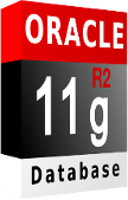
\includegraphics[scale=1]{oracle_11g}
\end{minipage}
\begin{minipage}[c]{0.8\textwidth}
    So wird das Ergebnis in einer Oracle 11g R2 Datenbank dargestellt.
\end{minipage}
\vfil
\begin{minipage}[c]{2cm}
    
\includegraphics[scale=1]{ms_sql}
\end{minipage}
\begin{minipage}[c]{0.8\textwidth}
    So wird das Ergebnis in einem Mircrosoft SQL Server 2008 R2 dargestellt.
\end{minipage}
\vfil
\begin{minipage}[c]{2cm}
    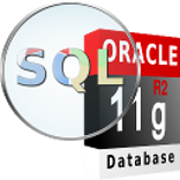
\includegraphics[scale=1]{ms_sql_oracle}
\end{minipage}
\begin{minipage}[c]{0.8\textwidth}
    Oracle und Microsoft SQL Server stellen das Ergebnis auf die gleiche Art und Weise dar.
\end{minipage}
\vfil

Eine solche Abfrage lässt sich nun um beliebige Spalten erweitern.
\begin{lstlisting}[language=oracle_sql,caption={Eine einfache Auswahlabfrage in Oracle},label=sql01_03]
SELECT Vorname, Nachname, Geburtsdatum, SozVersNr
FROM   Mitarbeiter;
        \end{lstlisting}
\clearpage
\begin{center}
    \begin{small}
        \changefont{pcr}{m}{n}
        \tablefirsthead{
            \multicolumn{1}{l}{\textbf{VORNAME}} &
            \multicolumn{1}{l}{\textbf{NACHNAME}} &
            \multicolumn{1}{l}{\textbf{GEBURTSDATUM}} &
            \multicolumn{1}{l}{\textbf{SOZVERSNR}} \\
            \cmidrule(l){1-1}\cmidrule(l){2-2}\cmidrule(l){3-3}\cmidrule(l){4-4}
        }
        %             \tabletail{
        %               \multicolumn{4}{l}{\textbf{100 Zeilen ausgewählt}} \\
        %             }
        \tablelasttail{
            \multicolumn{4}{l}{\textbf{100 Zeilen ausgewählt}} \\
        }
        \begin{msoraclesql}
            \begin{supertabular}{llll}
                Max & Winter & 31.08.88 & D370941F-6CD-6C07977\\
                Sarah & Werner & 03.11.77 & 18FE2247-C53-7EAD1ED\\
                Finn & Seifert & 17.10.85 & C973A840-B92-C5B97CD\\
                Sebastian & Schwarz & 27.06.92 & E8F8587D-CBA-0F28A80\\
                Tim & Sindermann & 11.01.80 & 703838BD-E9C-BD118A6\\
            \end{supertabular}
        \end{msoraclesql}
    \end{small}
\end{center}
\subsection{Der * als Joker}
In verschiedenen Kartenspielen gibt es Karten, die als Joker dienen. Solche \enquote{Universalkarten} können sich, in der richtigen Situation ausgespielt, als sehr nützlich erweisen. Auch in SQL gibt es einen Joker, den Stern *. Er ist immer dann dienlich, wenn man die Spaltenstruktur einer Tabelle nicht kennt oder einfach alle Spalten ausgeben möchte.
\begin{lstlisting}[language=oracle_sql,caption={Der * als Joker},label=sql01_04]
SELECT *
FROM   Bankfiliale;
        \end{lstlisting}
\begin{center}
    \begin{small}
        \changefont{pcr}{m}{n}
        \tablefirsthead{
            \multicolumn{1}{l}{\textbf{BANKFILIALE\_ID}} &
            \multicolumn{1}{l}{\textbf{STRASSE}} &
            \multicolumn{1}{l}{\textbf{HAUSNUMMER}} &
            \multicolumn{1}{l}{\textbf{PLZ}} &
            \multicolumn{1}{l}{\textbf{ORT}} \\
            \cmidrule(l){1-1}\cmidrule(l){2-2}\cmidrule(l){3-3}\cmidrule(l){4-4}\cmidrule(l){5-5}
        }
        \tabletail{
            \multicolumn{5}{l}{\textbf{21 Zeilen ausgewählt}} \\
        }
        \tablelasttail{
            \multicolumn{5}{l}{\textbf{21 Zeilen ausgewählt}} \\
        }
        \begin{msoraclesql}
            \begin{supertabular}{rllll}
                1 & Poststraße & 1 & 06449 & Aschersleben\\
                2 & Markt & 5 & 06449 & Aschersleben\\
                3 & Goethestraße & 4 & 39240 & Calbe\\
                4 & Lessingstraße & 1 & 06406 & Bernburg\\
                5 & Schillerstraße & 7 & 39240 & Barby\\
                6 & Kirchstraße & 8 & 39444 & Hecklingen\\
                7 & Ringstraße & 10 & 06420 & Könnern\\
            \end{supertabular}
        \end{msoraclesql}
    \end{small}
\end{center}
\begin{merke}
    Der Stern * dient, in der SELECT-Liste einer Auswahlabfrage, als Platzhalter, stellvertretend für alle Spalten einer Tabelle.
\end{merke}
Sollen alle Spalten, bis auf eine einzige angezeigt werden, kann der Stern leider nicht weiterhelfen. Eine Formulierung wie \enquote{* -1} ist nicht möglich. In einem solchen Fall müssen alle Spalten, bis auf die betreffende angegeben werden.
\subsection{Arithmetische Ausdrücke}
SQL ist, wie viele andere Programmiersprachen auch, in der Lage arithmetische Ausdrücke zu berechnen. Diese können nicht nur in der SELECT-Liste des SQL-Statements, sondern auch in verschiedenen anderen Klauseln, vorkommen. Die Syntax solcher Ausdrücke unterscheidet sich in Oracle und SQL Server nicht.
\begin{center}
    \tablecaption{Arithmetische Operatoren in Oracle und SQL Server}
    \tablefirsthead{
        \multicolumn{1}{c}{\textbf{(Operator)}} &
        \multicolumn{1}{c}{\textbf{(Bedeutung)}} \\
        \hline
    }
    \tabletail{
        \hline
    }
    \tablelasttail {
        \hline
    }
    \begin{supertabular}{ll}
        + & Addition \\
        - & Subtraktion \\
        * & Multiplikation \\
        / & Division \\
        \%& Modulo (Nur SQL-Server)\\
        . & Dezimaltrennzeichen\\
    \end{supertabular}
\end{center}

\beispiel{sql01_05} zeigt ein einfaches Anwendungsbeispiel. Für die Entscheidung über die Gehaltserhöhung der Mitarbeiter, ist es notwendig, im Vorfeld eine Auswertung zu erstellen, die zeigt, wie sich die Erhöhung von 2,5 \% auf die aktuellen Gehälter auswirkt.

\begin{lstlisting}[language=oracle_sql,caption={Arithmetische Ausdrücke in SQL},label=sql01_05]
SELECT Mitarbeiter_ID, Nachname, Gehalt, Gehalt * 1.025
FROM   Mitarbeiter;
        \end{lstlisting}
\begin{center}
    \begin{small}
        \changefont{pcr}{m}{n}
        \tablefirsthead {
            \multicolumn{1}{r}{\textbf{MITARBEITER\_ID}} &
            \multicolumn{1}{l}{\textbf{NACHNAME}} &
            \multicolumn{1}{r}{\textbf{GEHALT}} &
            \multicolumn{1}{r}{\textbf{GEHALT*1.025}} \\
            \cmidrule(r){1-1}\cmidrule(r){2-2}\cmidrule(r){3-3}\cmidrule(r){4-4}
        }
        \tablehead{}
        \tabletail {
            \multicolumn{4}{l}{\textbf{100 Zeilen ausgewählt}} \\
        }
        \tablelasttail {
            \multicolumn{4}{l}{\textbf{100 Zeilen ausgewählt}} \\
        }
        \begin{oraclesql}
            \begin{supertabular}{rlrr}
                1 & Winter & 88000 & 90200 \\
                2 & Werner & 50000 & 51250 \\
                3 & Seifert & 50000 & 51250 \\
                4 & Schwarz & 30000 & 30750 \\
                5 & Sindermann & 30000 & 30750 \\
                6 & Müller & 30000 & 30750 \\
            \end{supertabular}
        \end{oraclesql}
    \end{small}
\end{center}
\clearpage
\begin{center}
    \begin{small}
        \changefont{pcr}{m}{n}
        \tablefirsthead {
            \multicolumn{1}{r}{\textbf{MITARBEITER\_ID}} &
            \multicolumn{1}{l}{\textbf{NACHNAME}} &
            \multicolumn{1}{r}{\textbf{GEHALT}} &
            \multicolumn{1}{r}{\textbf{GEHALT*1.025}} \\
            \cmidrule(r){1-1}\cmidrule(r){2-2}\cmidrule(r){3-3}\cmidrule(r){4-4}
        }
        \tablehead{}
        \tabletail {
            \multicolumn{4}{l}{\textbf{100 Zeilen ausgewählt}} \\
        }
        \tablelasttail {
            \multicolumn{4}{l}{\textbf{100 Zeilen ausgewählt}} \\
        }
        \begin{mssql}
            \begin{supertabular}{llll}
                1 & Winter & 88000 & 90200 \\
                2 & Werner & 50000 & 51250 \\
                3 & Seifert & 50000 & 51250 \\
                4 & Schwarz & 30000 & 30750 \\
                5 & Sindermann & 30000 & 30750 \\
                6 & Müller & 30000 & 30750 \\
            \end{supertabular}
        \end{mssql}
    \end{small}
\end{center}
\begin{merke}
    Oracle und SQL Server unterscheiden sich in der Anzeige von numerischen Werten. Oracle stellt Zahlen immer rechtsbündig dar. SQL Server zeigt dagegen alle Werte linksbündig an.
\end{merke}
\subsection{NULL Werte}
\label{nullvalues}
Es kommt vor, dass nicht immer alle Attribute eines Datensatzes befüllt sind, d. h. einige Attribute haben keinen Attributwert. Dies kann aus zwei Gründen der Fall sein:
\begin{itemize}
    \item Der Wert eines Attributes ist zum Zeitpunkt der Eingabe des Datensatzes nicht bekannt (z. B. der Vorname einer Person ist nicht bekannt).
    \item Der Wert eines Attributs steht zum Zeitpunkt der Eingabe des Datensatzes noch nicht fest (z. B. das Sterbedatum einer Person bei der Erstellung der Geburtsurkunde).
\end{itemize}
\begin{merke}
    Ein NULL Wert steht immer für einen unbekannten Wert und ist nicht mit der natürlichen Zahl 0 zu verwechseln.
\end{merke}
NULL Werte haben insbesondere bei der Verwendung arithmetischer Ausdrücke eine große Bedeutung. Um dies zu demonstrieren, soll für alle Mitarbeiter deren Monatsgehalt berechnet werden. Dieses setzt sich aus dem Grundgehalt (Spalte \identifier{gehalt}) und einer Provision (Spalten \identifier{provision})zusammen. Da nicht jeder Mitarbeiter eine Provision erhält, existieren NULL Werte in der Tabelle \identifier{Mitarbeiter}.
\begin{lstlisting}[language=oracle_sql,caption={NULL in arithmetischen Ausdrücken},label=sql01_06]
SELECT Vorname, Nachname, Gehalt + Gehalt / 100 * Provision
FROM   Mitarbeiter;
        \end{lstlisting}
\clearpage
\begin{center}
    \begin{small}
        \changefont{pcr}{m}{n}
        \tablefirsthead {
            \multicolumn{1}{l}{\textbf{VORNAME}} &
            \multicolumn{1}{l}{\textbf{NACHNAME}} &
            \multicolumn{1}{r}{\textbf{GEHALT+GEHALT/100*PROVISION}} \\
            \cmidrule(l){1-1}\cmidrule(l){2-2}\cmidrule(l){3-3}
        }
        \tablehead{}
        \tabletail {
            \multicolumn{3}{l}{\textbf{100 Zeilen ausgewählt}} \\
        }
        \tablelasttail {
            \multicolumn{3}{l}{\textbf{100 Zeilen ausgewählt}} \\
        }
        \begin{oraclesql}
            \begin{supertabular}{llr}
                Max & Winter &  \\
                Sarah & Werner &  \\
                ... & ... & ... \\
                Johannes & Lehmann & 2400 \\
                Louis & Schmitz & 2500 \\
                Martin & Schacke & 1200 \\
            \end{supertabular}
        \end{oraclesql}
    \end{small}
\end{center}
\begin{merke}
    Einige Mitarbeiter erhalten keine Provision. Oracle und SQL Server unterscheiden sich bei der Anzeige der NULL Werte. Oracle zeigt für NULL Werte nichts an. SQL Server zeigt die Zeichenkette NULL an.
\end{merke}
Und hier das Ergebnis für den MS SQL Server.
\begin{center}
    \begin{small}
        \changefont{pcr}{m}{n}
        \tablefirsthead {
            \multicolumn{1}{l}{\textbf{VORNAME}} &
            \multicolumn{1}{l}{\textbf{NACHNAME}} &
            \multicolumn{1}{r}{\textbf{(Kein Spaltenname)}} \\
            \cmidrule(l){1-1}\cmidrule(l){2-2}\cmidrule(l){3-3}
        }
        \tablehead{}
        \tabletail {
            \multicolumn{3}{l}{\textbf{100 Zeilen ausgewählt}} \\
        }
        \tablelasttail {
            \multicolumn{3}{l}{\textbf{100 Zeilen ausgewählt}} \\
        }
        \begin{mssql}
            \begin{supertabular}{llr}
                Max & Winter &  NULL \\
                Sarah & Werner &  NULL \\
                Finn & Seifert &  NULL \\
                ... & ... & ... \\
                Johannes & Lehmann & 2400 \\
                Louis & Schmitz & 2500 \\
                Marie & Kipp &  NULL \\
                Amelie & Krüger &  NULL \\
                Martin & Schacke & 1200 \\
                ... & ... & ... \\
            \end{supertabular}
        \end{mssql}
    \end{small}
\end{center}
\begin{merke}
    Jeder arithmetische Ausdruck, in dem ein NULL Wert als Operand vorkommt, hat als Ergebnis den Wert NULL.
\end{merke}
\subsection{Verkettung von Zeichenketten}
In manchen Fällen ist es notwendig, die Ausgabe einzelner Spalten miteinander zu verbinden. Dieser Vorgang wird als Konkatenation\footnote{Verkettung von Zeichen oder Zeichenketten} bezeichnet. Hierfür kennt Oracle den Operator \textbardbl{} und SQL Server den Operator +.

\beispiel{sql01_05} wird nun dahingehend erweitert, dass die Gehaltserhöhung als Bericht angezeigt wird. Für jeden Mitarbeiter muss eine Zeile der Form \enquote{AAA hat ein Gehalt von XXX EUR und soll YYY EUR erhalten.}
\begin{lstlisting}[language=oracle_sql,caption={Verkettung von Zeichenketten in Oracle},label=sql01_07]
SELECT Nachname || ' hat ein Gehalt von ' || Gehalt ||
       ' EUR und soll ' || (Gehalt * 1.025) ||
       ' EUR erhalten.'
FROM   Mitarbeiter;
        \end{lstlisting}
\begin{center}
    \begin{small}
        \changefont{pcr}{m}{n}
        \tablefirsthead {
            \multicolumn{1}{l}{\textbf{NACHNAME||'HATEINGEHALTVON'||GEHALT||'EURUNDSOL...'}} \\
            \cmidrule(l){1-1}
        }
        \tablehead{}
        \tabletail {
            \multicolumn{1}{l}{\textbf{100 Zeilen ausgewählt}} \\
        }
        \tablelasttail {}
        \begin{oraclesql}
            \begin{supertabular}{l}
                Winter hat ein Gehalt von 88000 EUR und soll 90200 EUR erhalten. \\
                \dots \\
                Lehmann hat ein Gehalt von 2000 EUR und soll 2050 EUR erhalten. \\
                Schmitz hat ein Gehalt von 2000 EUR und soll 2050 EUR erhalten. \\
                Kipp hat ein Gehalt von 2000 EUR und soll 2050 EUR erhalten. \\
                \dots \\
            \end{supertabular}
        \end{oraclesql}
    \end{small}
\end{center}
\begin{lstlisting}[language=ms_sql,caption={Verkettung von Zeichenketten in SQL Server},label=sql01_08]
SELECT Nachname + ' hat ein Gehalt von '+ CAST(Gehalt AS VARCHAR(15)) +
       ' EUR und soll ' +
       CAST(Gehalt * 1.025 AS VARCHAR(15)) + ' erhalten.'
FROM   Mitarbeiter;
        \end{lstlisting}
\begin{center}
    \begin{small}
        \changefont{pcr}{m}{n}
        \tablefirsthead {
            \multicolumn{1}{l}{\textbf{(Kein Spaltenname)}} \\
            \cmidrule(l){1-1}
        }
        \tablehead{}
        \tabletail {
            \multicolumn{1}{l}{\textbf{100 Zeilen ausgewählt}} \\
        }
        \tablelasttail {
            \multicolumn{1}{l}{\textbf{100 Zeilen ausgewählt}} \\
        }
        \begin{mssql}
            \begin{supertabular}{l}
                Winter hat ein Gehalt von 88000 EUR und soll 90200 EUR erhalten. \\
                ... \\
                Lehmann hat ein Gehalt von 2000.00 EUR und soll ...  \\
                Schmitz hat ein Gehalt von 2000.00 EUR und soll ...  \\
                ... \\
                Schacke hat ein Gehalt von 1000.00 EUR und soll 1025 EUR erhalten. \\
                ... \\
            \end{supertabular}
        \end{mssql}
    \end{small}
\end{center}
An \beispiel{sql01_07} und \beispiel{sql01_08} sieht man sehr gut die unterschiedliche Reaktionsweise beider Datenbank Management Systeme. Oracle ist ohne weiteres in der Lage, Daten unterschiedlichen Typs (Zeichenketten, Zahl, Datumswerte, usw.) miteinander zu verknüpfen.

Bei Microsoft SQL Server ist dies nicht der Fall. Hier muss ein Vorgriff auf spätere Kapitel erfolgen. Der Zahlenwert der aus der Berechnung \textit{gehalt * 1.025} resultiert, muss explizit in eine Zeichenkette umgewandelt werden, bevor die Verkettung funktioniert.
\subsection{Spaltenaliasnamen}
Bei der Anzeige des Ergebnisses einer Auswahlabfrage wird für jede Spalte eine Überschrift erzeugt. Oracle und Microsoft SQL Server sind sich dabei in sofern einig, als dass für die Spaltenüberschriften die Spaltenbezeichner der Tabellenspalten genutzt werden. Wird aber in der \languageorasql{SELECT}-Liste eine Konstante, eine Funktion oder ein anderer Ausdruck genutzt, scheiden sich die Geister. SQL Server zeigt in so einem Falle einfach gar keine Überschrift an, während Oracle einen Teil des Ausdrucks als Überschrift nutzt. Dieses Verhalten ist in den vorangegangenen Beispielen an einigen Stellen zu sehen.

Der SQL-Standard erlaubt es dieses Verhalten zu beeinflussen und manuell eine Spaltenüberschrift, einen sogenannten \enquote{Spaltenaliasnamen}, zu vergeben. Dies funktioniert im Falle von Oracle und SQL Server auf die gleiche Art und Weise, da sich hier beide an den Standard halten.
\begin{lstlisting}[language=oracle_sql,caption={Vergabe eines Spaltenaliasnamen},label=sql01_09]
SELECT Vorname, Nachname, Gehalt + Gehalt / 100 * Provision AS "Neues Gehalt"
FROM   Mitarbeiter;
        \end{lstlisting}
\begin{center}
    \begin{small}
        \changefont{pcr}{m}{n}
        \tablefirsthead {
            \multicolumn{1}{l}{\textbf{VORNAME}} &
            \multicolumn{1}{l}{\textbf{NACHNAME}} &
            \multicolumn{1}{r}{\textbf{Neues Gehalt}} \\
            \cmidrule(l){1-1}\cmidrule(l){2-2}\cmidrule(l){3-3}
        }
        \tablehead{}
        \tabletail {
            \multicolumn{3}{l}{\textbf{100 Zeilen ausgewählt}} \\
        }
        \tablelasttail {
            \multicolumn{3}{l}{\textbf{100 Zeilen ausgewählt}} \\
        }
        \begin{msoraclesql}
            \begin{supertabular}{llr}
                ... & ... & ... \\
                Johannes & Lehmann & 2400 \\
                Louis & Schmitz & 2500 \\
                Marie & Kipp &  \\
                Amelie & Krüger &  \\
                Stefan & Beck &  \\
                Martin & Schacke & 1200 \\
                ... & ... & ... \\
            \end{supertabular}
        \end{msoraclesql}
    \end{small}
\end{center}

Der ANSI SQL-Standard sieht vier verschiedene Möglichkeiten zur Angabe eines Spaltenaliasnamen vor:
\begin{itemize}
    \item \languageorasql{[Ausdruck] AS "Spaltenaliasname"}
    \item \languageorasql{[Ausdruck] "Spaltenaliasname"}
    \item \languageorasql{[Ausdruck] Spaltenaliasname}
    \item \languageorasql{[Ausdruck] AS Spaltenaliasname}
\end{itemize}
Oracle und MS SQL Server unterstützen alle vier Varianten. Die Angabe von Anführungszeichen ist nur dann notwendig, wenn im Spaltenaliasnamen Sonderzeichen oder Leerzeichen vorkommen.
\begin{merke}
    Oracle wandelt einen Spaltenaliasnamen automatisch in Großbuchstaben um, es sei den, er wird in Anführungszeichen eingeschlossen.
\end{merke}
\section{Einige Konventionen zu SQL}
Um die Lesbarkeit von SQL-Statements zu verbessern werden an dieser Stelle einige Konventionen genannt, die im praktischen Umgang mit SQL eingehalten werden sollten.
\begin{itemize}
    \item Da SQL-Anweisungen mehrzeilig sein können erhält jede Klausel (SELECT, FROM, usw.) eine eigene Zeile.
    \item SQL ist nicht casesensitiv, d. h. Groß- und Kleinschreibung ist nicht relevant. Zur Verbesserung der Lesbarkeit sollten Schlüsselwörter groß geschrieben werden. Beispiele hierfür sind im gesamten Skript zu finden.
    \item Verwenden Sie Einrückungen zur Verbesserung der Lesbarkeit.
          \begin{lstlisting}[language=ms_sql,caption={So nicht!},label=sql01_10]
SELECT Nachname + ' hat ein Gehalt von  '+
CAST(Gehalt AS VARCHAR(15)) +
' EUR und soll ' +
CAST(Gehalt + Gehalt / 100 * Provision AS VARCHAR(15)) + ' erhalten.'
FROM   Mitarbeiter;
          \end{lstlisting}
          \begin{lstlisting}[language=ms_sql,caption={Viel besser lesbar!},label=sql_01_11]
SELECT Nachname + ' hat ein Gehalt von  '+ CAST(Gehalt AS VARCHAR(15)) +
       ' EUR und soll ' +
       CAST(Gehalt + Gehalt / 100 * Provision AS VARCHAR(15)) + ' erhalten.'
FROM   Mitarbeiter;
          \end{lstlisting}
    \item Gemä\ss\ SQL-Standard muss jedes SQL-Statement mit einem Semikolon (;) abgeschlossen werden. Anwendungen wie der SQL*Developer, der JDeveloper oder das Management Studio verbergen diesen Sachverhalt jedoch.
\end{itemize}
\begin{merke}
    In SQL*Plus muss jedes SQL-Statement mit ; oder / abgeschlossen werden!
\end{merke}

  \chapter{Selektieren und Sortieren}
\chaptertoc{}
\cleardoubleevenpage

\section{Selektieren von Zeilen: Die WHERE-Klausel}
Im vorangegangenen Kapitel wurde gezeigt, wie mit den beiden SQL-Klauseln \languageorasql{SELECT} und \languageorasql{FROM} der gesamte Inhalt einer Tabelle angezeigt werden kann. Zusätzlich zu diesen beiden Klauseln wird nun die optionale \languageorasql{WHERE}-Klausel eingeführt, die eine Selektion der Datensätze ermöglicht. Diese kann einen beliebig komplexen Ausdruck enthalten, der dann das \enquote{Auswahlkriterium} für die Datensätze darstellt. Die Syntax der \languageorasql{WHERE}-Klausel lautet wie folgt:
\begin{lstlisting}[language=oracle_sql,caption={Die WHERE-Klausel},label=sql02_01]
WHERE <Ausdruck1> <Relationaler Operator> <Ausdruck2>
      \end{lstlisting}
\begin{merke}
    Der Begriff \enquote{Ausdruck} steht in der Programmierung für ein auf einen Kontext bezogenes, auswertbares Gebilde. Bei \textit{Ausdruck1} und \textit{Ausdruck2} kann es sich beispielsweise um Spaltenbezeichner, Funktionsaufrufe, arithmetische Berechnungen, Konstanten usw. handeln.
\end{merke}
\beispiel{sql02_01} zeigt insgesamt drei Ausdrücke:
\begin{itemize}
    \item \textit{<Ausdruck1>}
    \item \textit{<Ausdruck2>}
    \item \textit{<Ausdruck1>} <Relationaler Operator> \textit{<Ausdruck2>}
\end{itemize}
Nicht nur \textit{Ausdruck1} und \textit{Ausdruck2} sind Ausdrücke, sondern auch die Verbindung beider, mittels eines Operators, wird als Ausdruck betrachtet.

\begin{merke}
    Ein Operator ist ein mit einer Semantik belegtes Zeichen, dass eine genau definierte Operation darstellt. Operatoren werden meist in Gruppen eingeteilt, z. B. arithmetische Operatoren (+, - , *, /), relationale Operatoren, logische Operatoren, usw.
\end{merke}
\tabelle{relopersql} listet die in Oracle und MS SQL Server vorhandenen relationalen Operatoren auf.
\clearpage
\subsection{Relationale Operatoren}
\begin{center}
    \tablecaption{Relationale Operatoren in Oracle und MS SQL Server}
    \label{relopersql}
    \begin{small}
        \tablefirsthead{
            \multicolumn{1}{c}{\textbf{(Operator)}} &
            \multicolumn{1}{c}{\textbf{(Bedeutung)}} \\
            \hline
        }
        \tablehead {
            \multicolumn{1}{c}{\textbf{(Operator)}} &
            \multicolumn{1}{c}{\textbf{(Bedeutung)}} \\
            \hline
        }
        \tabletail{
            \hline
        }
        \tablelasttail {
            \hline
        }
        \begin{supertabular}{lp{10cm}}
            =               & Gleichheit \\
            !=              & Ungleichheit \\
            \textless       & Kleiner als \\
            \textless=      & Kleiner oder gleich \\
            \textgreater    & Größer als \\
            \textgreater=   & Größer oder gleich \\
            LIKE            & Ähnlichkeit zweier Zeichenketten \\
            IN              & Der linke Ausdruck befindet sich in einer Liste von Werten, die der rechte Ausdruck erzeugt.\\
            IS NULL         & Der linke Ausdruck liefert den Wert NULL zurück. \\
            BETWEEN A AND B & Der Wert des linken Ausdrucks liegt zwischen den Wertgrenzen A und B. Die Wertgrenzen A und B werden in das Intervall mit einbezogen.\\
        \end{supertabular}
    \end{small}
\end{center}
\subsubsection{Numerische Werte vergleichen}
Der Vergleich von numerischen Werten gestaltet sich sowohl in Oracle als auch im MS SQL Server sehr einfach.
\begin{lstlisting}[language=oracle_sql,caption={Gleichheit zweier numerischer Werte},label=sql02_02]
SELECT Vorname, Nachname
FROM   Mitarbeiter
WHERE  Mitarbeiter_ID = 5;
          \end{lstlisting}
\begin{center}
    \begin{small}
        \changefont{pcr}{m}{n}
        \tablefirsthead{
            \multicolumn{1}{l}{\textbf{VORNAME}} &
            \multicolumn{1}{l}{\textbf{NACHNAME}} \\
            \cmidrule(l){1-1}\cmidrule(l){2-2}
        }
        \tablehead{}
        \tabletail{
            \multicolumn{2}{l}{\textbf{1 Zeile ausgewählt}} \\
        }
        \tablelasttail{
            \multicolumn{2}{l}{\textbf{1 Zeile ausgewählt}} \\
        }
        \begin{msoraclesql}
            \begin{supertabular}{ll}
                Tim & Sindermann \\
            \end{supertabular}
        \end{msoraclesql}
    \end{small}
\end{center}
\begin{lstlisting}[language=oracle_sql,caption={Wert A größer oder gleich Wert B},label=sql02_03]
SELECT Vorname, Nachname, Gehalt
FROM   Mitarbeiter
WHERE  Mitarbeiter_ID >= 50;
          \end{lstlisting}
\clearpage
\begin{center}
    \begin{small}
        \changefont{pcr}{m}{n}
        \tablefirsthead{
            \multicolumn{1}{r}{\textbf{VORNAME}} &
            \multicolumn{1}{l}{\textbf{NACHNAME}} &
            \multicolumn{1}{l}{\textbf{GEHALT}} \\
            \cmidrule(l){1-1}\cmidrule(l){2-2}\cmidrule(r){3-3}
        }
        \tablehead{}
        \tabletail{
            \multicolumn{3}{l}{\textbf{51 Zeilen gewählt}} \\
        }
        \tablelasttail{
            \multicolumn{3}{l}{\textbf{51 Zeilen gewählt}} \\
        }
        \begin{msoraclesql}
            \begin{supertabular}{llr}
                Emilia &  Köhler & 2500 \\
                Karolin & Klingner & 2000 \\
                Chris & Roggatz & 3000 \\
                Christian & Haas & 2000 \\
                Jessica & Winkler & 2000 \\
                Anna & Keller & 2500 \\
                Johannes & Klingner & 2500 \\
                Emma & Krüger & 3500 \\
            \end{supertabular}
        \end{msoraclesql}
    \end{small}
\end{center}
\begin{lstlisting}[language=oracle_sql,caption={Prüfen eines Intevalls},label=sql02_04]
SELECT Mitarbeiter_ID, Vorname, Nachname
FROM   Mitarbeiter
WHERE  Mitarbeiter_ID BETWEEN 5 AND 9;
          \end{lstlisting}
\begin{center}
    \begin{small}
        \changefont{pcr}{m}{n}
        \tablefirsthead{
            \multicolumn{1}{r}{\textbf{MITARBEITER\_ID}} &
            \multicolumn{1}{l}{\textbf{VORNAME}} &
            \multicolumn{1}{l}{\textbf{NACHNNAME}} \\
            \cmidrule(r){1-1}\cmidrule(l){2-2}\cmidrule(l){3-3}
        }
        \tablehead{}
        \tabletail{
            \multicolumn{3}{l}{\textbf{5 Zeilen gewählt}} \\
        }
        \tablelasttail{
            \multicolumn{3}{l}{\textbf{5 Zeilen gewählt}} \\
        }
        \begin{msoraclesql}
            \begin{supertabular}{rll}
                5 & Tim & Sindermann \\
                6 & Peter & Müller \\
                7 & Emily & Meier \\
                8 & Dirk & Peters \\
                9 & Louis & Winter \\
            \end{supertabular}
        \end{msoraclesql}
    \end{small}
\end{center}
\begin{lstlisting}[language=oracle_sql,caption={Alle Zeilen aus einer Wertemenge anzeigen},label=sql02_05]
SELECT Mitarbeiter_ID, Vorname, Nachname
FROM   Mitarbeiter
WHERE  Mitarbeiter_ID IN (5, 7, 9);
          \end{lstlisting}
\begin{center}
    \begin{small}
        \changefont{pcr}{m}{n}
        \tablefirsthead{
            \multicolumn{1}{r}{\textbf{MITARBEITER\_ID}} &
            \multicolumn{1}{l}{\textbf{VORNAME}} &
            \multicolumn{1}{l}{\textbf{NACHNNAME}} \\
            \cmidrule(r){1-1}\cmidrule(l){2-2}\cmidrule(l){3-3}
        }
        \tablehead{}
        \tabletail{
            \multicolumn{3}{l}{\textbf{3 Zeilen gewählt}} \\
        }
        \tablelasttail{
            \multicolumn{3}{l}{\textbf{3 Zeilen gewählt}} \\
        }
        \begin{msoraclesql}
            \begin{supertabular}{rll}
                5 & Tim & Sindermann \\
                7 & Emily & Meier \\
                9 & Louis & Winter \\
            \end{supertabular}
        \end{msoraclesql}
    \end{small}
\end{center}
\clearpage
\subsubsection{Zeichenketten vergleichen}
\label{stringdiff}
Der Vergleich zweier Zeichenketten bringt, im Gegensatz zum Vergleich numerischer Werte, eine Schwierigkeit mit sich. Abhängig vom benutzten RDBMS\footnote{RDBMS = Relationales Datenbank Management System} werden Zeichenkettenvergleiche casesensitiv oder incasesensitiv durchgeführt. In Oracle beispielsweise ist \enquote{Oracle} ungleich \enquote{oracle} oder \enquote{ORACLE} ungleich \enquote{OrAcLe}. Der MS SQL Server hingegen verhält sich nicht casesensitiv. Für ihn sind alle vier Werte gleich.

\begin{lstlisting}[language=oracle_sql,caption={Ein einfacher Zeichenkettenvergleich},label=sql02_06]
SELECT Mitarbeiter_ID, Vorname, Nachname
FROM   Mitarbeiter
WHERE  Nachname = 'Scholz';
          \end{lstlisting}
\begin{center}
    \begin{small}
        \changefont{pcr}{m}{n}
        \tablefirsthead{
            \multicolumn{1}{r}{\textbf{MITARBEITER\_ID}} &
            \multicolumn{1}{l}{\textbf{VORNAME}} &
            \multicolumn{1}{l}{\textbf{NACHNAME}} \\
            \cmidrule(r){1-1}\cmidrule(l){2-2}\cmidrule(l){3-3}
        }
        \tablehead{}
        \tabletail{
        }
        \tablelasttail{
            \multicolumn{3}{l}{\textbf{1 Zeile ausgewählt}} \\
        }
        \begin{msoraclesql}
            \begin{supertabular}{rll}
                96 & Johanna & Scholz \\
            \end{supertabular}
        \end{msoraclesql}
    \end{small}
\end{center}
Im nächsten Beispiel wird eine ähnliche \languageorasql{WHERE}-Klausel verwendet, wie in \beispiel{sql02_06}, sie führt jedoch zu einem ganz anderen Ergebnis.

\begin{merke}
    In SQL müssen Zeichenketten in Hochkommas ' eingeschlossen werden! Diese dürfen nicht mit den Akzent-Zeichen verwechselt werden!
\end{merke}
\begin{lstlisting}[language=oracle_sql,caption={Ein einfacher Zeichenkettenvergleich},label=sql02_07]
SELECT Mitarbeiter_ID, Vorname, Nachname
FROM   Mitarbeiter
WHERE  Nachname = 'SCHOLZ';
          \end{lstlisting}
\begin{center}
    \begin{small}
        \changefont{pcr}{m}{n}
        \begin{oraclesql}
            Keine Zeilen ausgewählt!
        \end{oraclesql}
    \end{small}
\end{center}
Da die Oracle-Datenbank casesensitiv arbeitet, ist \enquote{SCHOLZ} ungleich \enquote{Scholz}. Somit werden keine Datensätze gefunden. Der MS SQL Server hat hier keine Schwierigkeiten. Ihn stört die unterschiedliche Schreibweise der Zeichenketten nicht, weshalb er das gewünschte Ergebnis anzeigt.
\clearpage
\begin{center}
    \begin{small}
        \changefont{pcr}{m}{n}
        \tablefirsthead{
            \multicolumn{1}{r}{\textbf{MITARBEITER\_ID}} &
            \multicolumn{1}{l}{\textbf{VORNAME}} &
            \multicolumn{1}{l}{\textbf{NACHNAME}} \\
            \cmidrule(r){1-1}\cmidrule(l){2-2}\cmidrule(l){3-3}
        }
        \tablehead{}
        \tabletail{
            \multicolumn{3}{l}{\textbf{1 Zeile ausgewählt}} \\
        }
        \tablelasttail{
            \multicolumn{3}{l}{\textbf{1 Zeile ausgewählt}} \\
        }
        \begin{mssql}
            \begin{supertabular}{rll}
                96 & Johanna & Scholz \\
            \end{supertabular}
        \end{mssql}
    \end{small}
\end{center}
\subsubsection{Zeichenketten vergleichen mit LIKE}
Ist es notwendig nach einem Zeichenmuster zu suchen, wie z. B. \textit{Alle Mitarbeiter, deren Nachname mit \enquote{Sch} beginnt}, so kann dies mit dem \languageorasql{LIKE}-Operator geschehen.
\begin{lstlisting}[language=oracle_sql,caption={Zeichenkettensuche mit einem Suchmuster},label=sql02_08]
SELECT Mitarbeiter_ID, Vorname, Nachname
FROM   Mitarbeiter
WHERE  Nachname LIKE 'Sch%';
          \end{lstlisting}
\begin{center}
    \begin{small}
        \changefont{pcr}{m}{n}
        \tablefirsthead{
            \multicolumn{1}{r}{\textbf{MITARBEITER\_ID}} &
            \multicolumn{1}{l}{\textbf{VORNAME}} &
            \multicolumn{1}{l}{\textbf{NACHNAME}} \\
            \cmidrule(r){1-1}\cmidrule(l){2-2}\cmidrule(l){3-3}
        }
        \tablehead{}
        \tabletail{
        }
        \tablelasttail{
            \multicolumn{1}{l}{\textbf{10 Zeilen ausgewählt}} \\
        }
        \begin{msoraclesql}
            \begin{supertabular}{rll}
                4 & Sebastian & Schwarz \\
                11 & Sophie & Schwarz \\
                25 & Elias & Schreiber \\
                29 & Louis & Schmitz \\
                33 & Martin & Schacke \\
                36 & Hans & Schumacher \\
            \end{supertabular}
        \end{msoraclesql}
    \end{small}
\end{center}
Der \languageorasql{LIKE}-Operator nutzt zwei Wildcards, um Suchmuster für Zeichenketten zu erstellen.
\begin{center}
    \tablecaption{Wildcards des LIKE-Operators}
    \label{likewildcards}
    \begin{small}
        \tablefirsthead{
            \multicolumn{1}{c}{\textbf{(Wildcard)}} &
            \multicolumn{1}{c}{\textbf{(Bedeutung)}} \\
            \hline
        }
        \tabletail{
            \hline
        }
        \tablelasttail{
            \hline
        }
        \begin{supertabular}{lp{10cm}}
            \% & (Prozentzeichen) Null, eines oder beliebig viele Zeichen \\
            \_ & (Unterstrich) Genau ein Zeichen \\
        \end{supertabular}
    \end{small}
\end{center}
Für \beispiel{sql02_08} bedeutet dies: \textit{Die ersten drei Zeichen des Suchmusters sind S, c und h. Nach dem h können null, eines oder beliebig viele andere Zeichen stehen.} Im nächsten Beispiel wird die \textit{\_}-Wildcard benutzt, um alle Mitarbeiter zu suchen, deren Nachname an der dritten Stelle ein kleines g trägt.
\begin{lstlisting}[language=oracle_sql,caption={Zeichenkettensuche mit einem etwas komplexeren Suchmuster},label=sql02_09]
SELECT Mitarbeiter_ID, Vorname, Nachname
FROM   Mitarbeiter
WHERE  Nachname LIKE '__g%';
          \end{lstlisting}
\clearpage
\begin{center}
    \begin{small}
        \changefont{pcr}{m}{n}
        \tablefirsthead{
            \multicolumn{1}{r}{\textbf{MITARBEITER\_ID}} &
            \multicolumn{1}{l}{\textbf{VORNAME}} &
            \multicolumn{1}{l}{\textbf{NACHNAME}} \\
            \cmidrule(r){1-1}\cmidrule(l){2-2}\cmidrule(l){3-3}
        }
        \tablehead{}
        \tabletail{
            \multicolumn{1}{l}{\textbf{4 Zeilen ausgewählt}} \\
        }
        \tablelasttail{
            \multicolumn{1}{l}{\textbf{4 Zeilen ausgewählt}} \\
        }
        \begin{msoraclesql}
            \begin{supertabular}{rll}
                37 & Louis & Wagner \\
                52 & Chris & Roggatz \\
                83 & Peter & Roggatz \\
                88 & Joachim & Wagner \\
            \end{supertabular}
        \end{msoraclesql}
    \end{small}
\end{center}
Die ersten beiden Zeichen des Suchmusters sind \textit{\_} Unterstriche, d. h. an der ersten und zweiten Stelle der gesuchten Zeichenketten \textbf{muss} sich jeweils genau ein Zeichen befinden. Das dritte Zeichen ist mit dem \textit{g} genau definiert. Anschließend können wieder null, eines oder beliebig viele andere Zeichen stehen.

\begin{merke}
    Der LIKE-Operator verwendet die beiden Wildcards \% und \_ . \% Steht für null, eines oder beliebig viele Zeichen. \_ steht für genau ein Zeichen.
\end{merke}
\subsubsection{Vergleiche mit NULL-Werten}
Sowohl Oracle, als auch der MS SQL Server kennen beide den Operator \languageorasql{IS NULL}. Mit seiner Hilfe können Spalten auf NULL-Werte hin überprüft werden. Sollen z. B. alle Mitarbeiter, die keinen Vorgesetzten haben, angezeigt werden, wird ein Vergleich mit dem \languageorasql{IS NULL}-Operator angestellt.
\begin{lstlisting}[language=oracle_sql,caption={Der IS NULL Operator},label=sql02_10]
SELECT Mitarbeiter_ID, Vorname, Nachname, Vorgesetzter_ID
FROM   Mitarbeiter
WHERE  Vorgesetzter_ID IS NULL;
          \end{lstlisting}
\begin{center}
    \begin{small}
        \changefont{pcr}{m}{n}
        \tablefirsthead{
            \multicolumn{1}{r}{\textbf{MITARBEITER\_ID}} &
            \multicolumn{1}{l}{\textbf{VORNAME}} &
            \multicolumn{1}{l}{\textbf{NACHNAME}} &
            \multicolumn{1}{r}{\textbf{VORGESETZTER\_ID}} \\
            \cmidrule(r){1-1}\cmidrule(l){2-2}\cmidrule(l){3-3}\cmidrule(r){4-4}
        }
        \tablehead{}
        \tabletail{
            \multicolumn{4}{l}{\textbf{1 Zeile ausgewählt}} \\
        }
        \tablelasttail{
            \multicolumn{4}{l}{\textbf{1 Zeile ausgewählt}} \\
        }
        \begin{msoraclesql}
            \begin{supertabular}{rllr}
                1 & Max & Winter & \\
            \end{supertabular}
        \end{msoraclesql}
    \end{small}
\end{center}
Da es in diesem Beispiel keinen wesentlichen Unterschied bei der Ergebnisanzeige zwischen Oracle und SQL Server gibt (SQL Server zeigt das Wort NULL für NULL-Werte und alle Spaltenwerte linksbündig an), wurde hier auf ein getrenntes Abdrucken der Ergebnisse verzichtet.

Das Gegenstück zum \languageorasql{IS NULL}-Operator, ist der \languageorasql{IS NOT NULL}-Operator.
\clearpage
\begin{merke}
    Wird ein Ausdruck, mit Hilfe des Gleichheitsoperators (=), mit dem Wert NULL verglichen, ist das Ergebnis des Vergleichs immer NULL!
\end{merke}
\subsection{Logische Verknüpfung von Ausdrücken}
In vielen Fällen ist es notwendig komplexe Ausdrücke zu formulieren, indem mehrere Ausdrücke miteinander verknüpft werden. Eine solche Verknüpfung geschieht unter Zuhilfenahme der logischen Operatoren \textit{AND}, \textit{OR} und \textit{NOT}.
\subsubsection{Logische Verknüpfungen mit AND}
Der logische Operator \textit{AND} verknüpft zwei Bedingungen miteinander und liefert ein wahres Ergebnis, sobald beide Ausdrücke ein wahres Ergebnis haben. Die Logiktabelle \tabelle{logikand} zeigt die möglichen Ergebnisse einer AND-Verknüpfung.
\vspace{\baselineskip}
\begin{center}
    \tablecaption{Der logische Operator AND}
    \label{logikand}
    \tablefirsthead{
        \multicolumn{1}{l}{\textbf{Aussagen}} &
        \multicolumn{1}{c}{\textbf{(Wahr)}} &
        \multicolumn{1}{c}{\textbf{(Falsch)}} \\
        \hline
    }
    \tablehead{}
    \tabletail{
        \hline
    }
    \tablelasttail{
        \hline
    }
    \begin{supertabular}{|l|c|c|}
        Wahr & w & f \\
        \hline
        Falsch & f & f \\
    \end{supertabular}
\end{center}
In \beispiel{sql02_11} wird gezeigt, wie der \textit{AND}-Operator dazu genutzt werden kann, um zwei Bedingungen miteinander zu verknüpfen. Es sollen alle Mitarbeiter angezeigt werden, deren Gehalt unter 1.500 EUR liegt und die in der Bankfiliale Nummer zwei arbeiten.
\begin{lstlisting}[language=oracle_sql,caption={Der AND Operator},label=sql02_11]
SELECT Vorname, Nachname, Gehalt, Bankfiliale_ID
FROM   Mitarbeiter
WHERE  Gehalt < 1500
  AND  Bankfiliale_ID = 2;
          \end{lstlisting}
\begin{center}
    \begin{small}
        \changefont{pcr}{m}{n}
        \tablefirsthead{
            \multicolumn{1}{l}{\textbf{VORNAME}} &
            \multicolumn{1}{l}{\textbf{NACHNAME}} &
            \multicolumn{1}{r}{\textbf{GEHALT}} &
            \multicolumn{1}{r}{\textbf{BANKFILIALE\_ID}}\\
            \cmidrule(l){1-1}\cmidrule(l){2-2}\cmidrule(r){3-3}\cmidrule(r){4-4}
        }
        \tablehead{}
        \tabletail{
            \multicolumn{1}{l}{\textbf{2 Zeilen ausgewählt}} \\
        }
        \tablelasttail{
            \multicolumn{1}{l}{\textbf{2 Zeilen ausgewählt}} \\
        }
        \begin{msoraclesql}
            \begin{supertabular}{llrr}
                Martin & Schacke & 1000 & 2 \\
                Oliver & Wolf & 1000 & 2 \\
            \end{supertabular}
        \end{msoraclesql}
    \end{small}
\end{center}
\subsubsection{Logische Verknüpfungen mit OR}
Der logische Operator \textit{OR} liefert, im Unterschied zu \textit{AND}, ein wahres Ergebnis, sobald mindestens einer der beiden Ausdrücke ein wahres Ergebnis hat.
\begin{center}
    \tablecaption{Der logische Operator OR}
    \label{logikor}
    \tablefirsthead{
        \multicolumn{1}{l}{\textbf{Aussagen}} &
        \multicolumn{1}{c}{\textbf{(Wahr)}} &
        \multicolumn{1}{c}{\textbf{(Falsch)}} \\
        \hline
    }
    \tablehead{}
    \tabletail{
        \hline
    }
    \tablelasttail{
        \hline
    }
    \begin{supertabular}{|l|c|c|}
        Wahr & w & w \\
        \hline
        Falsch & w & f \\
    \end{supertabular}
\end{center}
Wird in \beispiel{sql02_11} der Operator \textit{AND} durch ein \textit{OR} ersetzt, verändert sich die Ergebnismenge. Es werden jetzt alle Mitarbeiter angezeigt, die entweder ein Gehalt unter 1.500 EUR haben oder die in Bankfilialie Nummer zwei arbeiten.
\begin{lstlisting}[language=oracle_sql,caption={Der OR Operator},label=sql02_12]
SELECT Vorname, Nachname, Gehalt, Bankfiliale_ID
FROM   Mitarbeiter
WHERE  Gehalt < 1500
   OR  Bankfiliale_ID = 2;
          \end{lstlisting}
\begin{center}
    \begin{small}
        \changefont{pcr}{m}{n}
        \tablefirsthead{
            \multicolumn{1}{l}{\textbf{VORNAME}} &
            \multicolumn{1}{l}{\textbf{NACHNAME}} &
            \multicolumn{1}{r}{\textbf{GEHALT}} &
            \multicolumn{1}{r}{\textbf{BANKFILIALE\_ID}}\\
            \cmidrule(l){1-1}\cmidrule(l){2-2}\cmidrule(l){3-3}\cmidrule(l){4-4}
        }
        \tablehead{}
        \tabletail{
            \multicolumn{1}{l}{\textbf{9 Zeilen ausgewählt}} \\
        }
        \tablelasttail{
            \multicolumn{1}{l}{\textbf{9 Zeilen ausgewählt}} \\
        }
        \begin{msoraclesql}
            \begin{supertabular}{llrr}
                Louis & Winter & 12000 & 2 \\
                Stefan & Beck & 1500 & 2 \\
                Martin & Schacke & 1000 & 2 \\
                Max & Oswald & 1500 & 2 \\
                Oliver & Wolf & 1000 & 2 \\
                Hans & Schumacher & 1000 & 3 \\
                Maja & Keller & 1000 & 5 \\
                Elias & Sindermann & 1000 & 8 \\
                Jonas & Meier & 1000 & 12 \\
            \end{supertabular}
        \end{msoraclesql}
    \end{small}
\end{center}
\subsubsection{Aussagen mit NOT umkehren}
Die Bedeutung des Operators \textit{NOT} ist sehr einfach zu umschreiben. Er kehrt ein Ergebnis um. Aus einem wahren Ergebnis wird ein falsches und umgekehrt. Dieser Effekt ist auch mit \languageorasql{IS NULL} und \languageorasql{IS NOT NULL} zu sehen. In \beispiel{sql02_13} werden alle Mitarbeiter angezeigt, deren Gehalt kleiner als 1.500 EUR ist und die nicht in der Bankfiliale Nummer zwei arbeiten.
\begin{lstlisting}[language=oracle_sql,caption={Der NOT Operator},label=sql02_13]
SELECT Vorname, Nachname, Gehalt, Bankfiliale_ID
FROM   Mitarbeiter
WHERE  Gehalt < 1500
  AND  NOT Bankfiliale_ID = 2;
          \end{lstlisting}
\begin{center}
    \begin{small}
        \changefont{pcr}{m}{n}
        \tablefirsthead{
            \multicolumn{1}{l}{\textbf{VORNAME}} &
            \multicolumn{1}{l}{\textbf{NACHNAME}} &
            \multicolumn{1}{r}{\textbf{GEHALT}} &
            \multicolumn{1}{r}{\textbf{BANKFILIALE\_ID}}\\
            \cmidrule(l){1-1}\cmidrule(l){2-2}\cmidrule(r){3-3}\cmidrule(r){4-4}
        }
        \tablehead{}
        \tabletail{
            \multicolumn{1}{l}{\textbf{4 Zeilen ausgewählt}} \\
        }
        \tablelasttail{
            \multicolumn{1}{l}{\textbf{4 Zeilen ausgewählt}} \\
        }
        \begin{msoraclesql}
            \begin{supertabular}{llrr}
                Hans & Schumacher & 1000 & 3 \\
                Maja & Keller & 1000 & 5 \\
                Elias & Sindermann & 1000 & 8 \\
                Jonas & Meier & 1000 & 12 \\
            \end{supertabular}
        \end{msoraclesql}
    \end{small}
\end{center}
\begin{merke}
    Die Klammern ( und ) haben Einfluss auf die Bedeutung von Ausdrücken. Werden mehrere logische Operatoren kombiniert, kann so die Lesbarkeit von Ausdrücken verbessert oder deren Bedeutung verändert werden.
\end{merke}
\section{Festlegen einer Sortierung}
In allen vorangegangenen Beispielen war die Reihenfolge der Ausgabe der Datensätze unbestimmt. Sowohl Oracle als auch Microsoft SQL Server geben die Datensätze immer in der Reihenfolge aus, in der sie in der Quelltabelle vorliegen. Soll eine sortierte Ausgabe erfolgen, muss dies mit Hilfe der in \beispiel{sql01_01} gezeigten \languageorasql{ORDER BY}-Klausel geschehen. Dazu muss diese, mit Sortierbegriffen versehen, am Ende des SQL-Statements angegeben werden.
\subsection{Die ORDER BY Klausel}
\begin{lstlisting}[language=oracle_sql,caption={Die ORDER BY Klausel},label=sql02_14]
ORDER BY <Sortierbegriff 1> [asc|desc],
         <Sortierbegriff 2> [asc|desc],
         <Sortierbegriff n> [asc|desc] ...
        \end{lstlisting}
Als Sortierbegriffe können Spaltenbezeichner, Spaltenaliasnamen, berechnete Ausdrücke und auch Spaltenpositionsangaben, bezogen auf die Reihenfolge der Spaltennamen in der SELECT-Liste, genutzt werden. \beispiel{sql02_15} und \beispiel{sql02_16} zeigen die Anwendung der \languageorasql{ORDER BY}-Klausel.
\clearpage
\begin{merke}
    Werden mehrere Sortierbegriffe angegeben, wird die Sortierung von links nach rechts durchgeführt. Das bedeutet, dass zuerst nach dem äußerst linken Sortierbegriff sortiert wird und anschließend wird, innerhalb dieser Sortierung, jeder weitere Sortierbegriff angewandt. Die Sortierungen werden also ineinander geschachtelt.
\end{merke}
\begin{lstlisting}[language=oracle_sql,caption={Die ORDER BY Klausel mit Spaltenbezeichnern},label=sql02_15]
SELECT   Vorname, Nachname, Gehalt, Bankfiliale_ID
FROM     Mitarbeiter
WHERE    Gehalt <= 1500
ORDER BY Gehalt;
        \end{lstlisting}
\begin{center}
    \begin{small}
        \changefont{pcr}{m}{n}
        \tablefirsthead{
            \multicolumn{1}{l}{\textbf{VORNAME}} &
            \multicolumn{1}{l}{\textbf{NACHNAME}} &
            \multicolumn{1}{r}{\textbf{GEHALT}} &
            \multicolumn{1}{r}{\textbf{BANKFILIALE\_ID}}\\
            \cmidrule(l){1-1}\cmidrule(l){2-2}\cmidrule(l){3-3}\cmidrule(l){4-4}
        }
        \tablehead{}
        \tabletail{
            \multicolumn{1}{l}{\textbf{18 Zeilen ausgewählt}} \\
        }
        \tablelasttail{
            \multicolumn{1}{l}{\textbf{18 Zeilen ausgewählt}} \\
        }
        \begin{msoraclesql}
            \begin{supertabular}{llrr}
                Oliver & Wolf & 1000 & 2 \\
                Hans & Schumacher & 1000 & 3 \\
                Maja & Wolf & 1000 & 5 \\
                Elias & Sindermann & 1000 & 8 \\
                Jonas & Meier & 1000 & 12 \\
                Martin & Schacke & 1000 & 2 \\
                Max & Oswald & 1500 & 2 \\
                Stefan & Beck & 1500 & 2\\
            \end{supertabular}
        \end{msoraclesql}
    \end{small}
\end{center}
\begin{lstlisting}[language=oracle_sql,caption={Die ORDER BY Klausel mit Positionsangaben},label=sql02_16]
SELECT   Vorname, Nachname, Gehalt, Bankfiliale_ID
FROM     Mitarbeiter
WHERE    Gehalt <= 1500
ORDER BY 3, 2;
        \end{lstlisting}
\begin{center}
    \begin{small}
        \changefont{pcr}{m}{n}
        \tablefirsthead{
            \multicolumn{1}{l}{\textbf{VORNAME}} &
            \multicolumn{1}{l}{\textbf{NACHNAME}} &
            \multicolumn{1}{r}{\textbf{GEHALT}} &
            \multicolumn{1}{r}{\textbf{BANKFILIALE\_ID}}\\
            \cmidrule(l){1-1}\cmidrule(l){2-2}\cmidrule(l){3-3}\cmidrule(l){4-4}
        }
        \tablehead{}
        \tabletail{
            %               \multicolumn{1}{l}{\textbf{18 Zeilen ausgewählt}} \\
        }
        \tablelasttail{
            \multicolumn{1}{l}{\textbf{18 Zeilen ausgewählt}} \\
        }
        \begin{msoraclesql}
            \begin{supertabular}{llrr}
                Maja & Keller & 1000 & 5 \\
                Jonas & Meier & 1000 & 12 \\
                Martin & Schacke & 1000 & 2 \\
                Hans & Schumacher & 1000 & 3 \\
                Elias & Sindermann & 1000 & 8 \\
                Oliver & Wolf & 1000 & 2 \\
                Stefan & Beck & 1500 & 2 \\
                Georg & Dühning & 1500 & 20 \\
            \end{supertabular}
        \end{msoraclesql}
    \end{small}
\end{center}
\clearpage
\begin{merke}
    Bei der Benutzung von Positionsangaben (siehe \beispiel{sql02_16}) muss darauf geachtet werden, dass sich diese auf die Reihenfolge der Spaltenbezeichner in der SELECT-Liste beziehen. Wird die SELECT-Liste später verändert, müssen unter Umständen auch die Positionsangaben angepasst werden.
\end{merke}
\subsection{Auf- und absteigendes Sortieren}
Zu jedem Suchbegriff können die beiden Kürzel \languageorasql{ASC} und \languageorasql{DESC} mit angegeben werden. \languageorasql{ASC}\footnote{engl. Ascending = aufsteigend} bewirkt aufsteigende Sortierung (Standard) und \languageorasql{DESC}\footnote{engl. Descending = absteigend} absteigende Sortierung. \beispiel{sql02_17} zeigt, wie sich das Ergebnis durch die absteigende Sortierung der Spalte \identifier{gehalt} verändert.
\begin{lstlisting}[language=oracle_sql,caption={Die ORDER BY Klausel mit absteigender Sortierung},label=sql02_17]
SELECT   Vorname, Nachname, Gehalt, Bankfiliale_ID
FROM     Mitarbeiter
WHERE    Gehalt <= 1500
ORDER BY Gehalt DESC, 2 ASC;
        \end{lstlisting}
\begin{center}
    \begin{small}
        \changefont{pcr}{m}{n}
        \tablefirsthead{
            \multicolumn{1}{l}{\textbf{VORNAME}} &
            \multicolumn{1}{l}{\textbf{NACHNAME}} &
            \multicolumn{1}{r}{\textbf{GEHALT}} &
            \multicolumn{1}{r}{\textbf{BANKFILIALE\_ID}}\\
            \cmidrule(l){1-1}\cmidrule(l){2-2}\cmidrule(l){3-3}\cmidrule(l){4-4}
        }
        \tablehead{}
        \tabletail{
            \multicolumn{1}{l}{\textbf{18 Zeilen ausgewählt}} \\
        }
        \tablelasttail{
            \multicolumn{1}{l}{\textbf{18 Zeilen ausgewählt}} \\
        }
        \begin{msoraclesql}
            \begin{supertabular}{llrr}
                Stefen & Beck & 1500 & 2 \\
                Georg & Dühning & 1500 & 20 \\
                Tom & Fischer & 1500 & 17 \\
                Jannis & Friedrich & 1500 & 14 \\
                Maximilian & Hahn & 1500 & 13 \\
                Lena & Hermann & 1500 & 4 \\
                Anne & Huber & 1500 & 10 \\
            \end{supertabular}
        \end{msoraclesql}
    \end{small}
\end{center}
\begin{merke}
    Eine in der \languageorasql{ORDER BY}-Klausel als Sortierbegriff genutzte Spalte, muss nicht in der SELECT-Liste der Abfrage vorhanden sein.
\end{merke}

    \clearpage
    \section{Übungen - Selektieren und Sortieren}
      \begin{enumerate}
        \item Erstellen Sie eine Abfrage, die die Konto\_ID und das aktuelle
        Guthaben des Girokontos der Bankkunden anzeigt, die weniger als 1000 EUR
        Guthaben besitzen.
        \begin{center}
          \begin{small}
            \changefont{pcr}{m}{n}
            \tablefirsthead {
              \multicolumn{1}{r}{\textbf{KONTO\_ID}} &
              \multicolumn{1}{r}{\textbf{GUTHABEN}} \\
              \cmidrule(r){1-1}\cmidrule(r){2-2}
            }
            \tablehead{}
            \tabletail {
              \multicolumn{2}{l}{\textbf{55 Zeilen ausgewählt}} \\
            }
            \tablelasttail {
              \multicolumn{2}{l}{\textbf{55 Zeilen ausgewählt}} \\
            }
            \begin{msoraclesql}
              \begin{supertabular}{rr}
                15 & -10496,4 \\
                16 & -54593,2 \\
                43 & -42144,1 \\
                48 & -140505,1 \\
                57 & -1088,4 \\
                59 & 760,1 \\
                83 & 336,2 \\
                87 & -9009,1 \\
                99 & -69705,6 \\
              \end{supertabular}
            \end{msoraclesql}
          \end{small}
        \end{center}
        \item Erstellen Sie eine Abfrage, die die Mitarbeiter\_ID und den
        Nachnamen der Mitarbeiter mit der Vorgesetzter\_ID \enquote{2} anzeigt.
        \begin{center}
          \begin{small}
            \changefont{pcr}{m}{n}
            \tablefirsthead {
              \multicolumn{1}{r}{\textbf{MITARBEITER\_ID}} &
              \multicolumn{1}{l}{\textbf{NACHNAME}} \\
              \cmidrule(r){1-1}\cmidrule(l){2-2}
            }
            \tablehead{}
            \tabletail {
              \multicolumn{2}{l}{\textbf{2 Zeilen ausgewählt}} \\
            }
            \tablelasttail {
              \multicolumn{2}{l}{\textbf{2 Zeilen ausgewählt}} \\
            }
            \begin{msoraclesql}
              \begin{supertabular}{rl}
                4 & Schwarz \\
                5 & Sindermann \\
              \end{supertabular}
            \end{msoraclesql}
          \end{small}
        \end{center}
        \item Erstellen Sie eine Abfrage, die die Konto\_ID und das aktuelle
        Guthaben des Girokontos der Bankkunden anzeigt, deren Guthaben nicht
        zwischen 1000 EUR und 1500 EUR liegt.
        \begin{center}
          \begin{small}
            \changefont{pcr}{m}{n}
            \tablefirsthead {
              \multicolumn{1}{r}{\textbf{KONTO\_ID}} &
              \multicolumn{1}{r}{\textbf{GUTHABEN}} \\
              \cmidrule(r){1-1}\cmidrule(r){2-2}
            }
            \tablehead{}
            \tabletail {
%               \multicolumn{2}{l}{\textbf{428 Zeilen ausgewählt}} \\
            }
            \tablelasttail {
              \multicolumn{2}{l}{\textbf{428 Zeilen ausgewählt}} \\
            }
            \begin{msoraclesql}
              \begin{supertabular}{rr}
                1 & 111316,9 \\
                2 & 96340,2 \\
                3 & 59633 \\
                5 & 98449 \\
                6 & 26130,7 \\
                7 & 23128,7 \\
                9 & 8857,6 \\
                10 & 68001,3 \\
              \end{supertabular}
            \end{msoraclesql}
          \end{small}
        \end{center}
\clearpage
        \item Lassen Sie sich die Kunden\_ID und das Geburtsdatum aller
        Eigenkunden anzeigen, die zwischen dem 20. Februar 1980 und dem 02.
        März 1988 geboren sind. Zusätzlich soll die Abfrage nach
        dem Geburtsdatum in aufsteigender Reihenfolge sortiert werden.
        \begin{center}
          \begin{small}
            \changefont{pcr}{m}{n}
            \tablefirsthead {
              \multicolumn{1}{r}{\textbf{KUNDEN\_ID}} &
              \multicolumn{1}{l}{\textbf{GEBURTSDATUM}} \\
              \cmidrule(r){1-1}\cmidrule(l){2-2}
            }
            \tablehead{}
            \tabletail {
              \multicolumn{2}{l}{\textbf{124 Zeilen ausgewählt}} \\
            }
            \tablelasttail {
              \multicolumn{2}{l}{\textbf{124 Zeilen ausgewählt}} \\
            }
            \begin{msoraclesql}
              \begin{supertabular}{rl}
                391 & 01.03.80 \\
                387 & 03.03.80 \\
                339 & 22.03.80 \\
                75 & 22.03.80 \\
                458 & 07.05.80 \\
                50 & 21.05.80 \\
              \end{supertabular}
            \end{msoraclesql}
          \end{small}
        \end{center}
        \item Zeigen Sie, in alphabetischer Reihenfolge, die Mitarbeiter\_ID und
        den Nachnamen der Mitarbeiter an, die die Vorgesetzter\_ID \enquote{5}
        oder \enquote{6} haben.
        \begin{center}
          \begin{small}
            \changefont{pcr}{m}{n}
            \tablefirsthead {
              \multicolumn{1}{r}{\textbf{MITARBEITER\_ID}} &
              \multicolumn{1}{l}{\textbf{NACHNAME}} \\
              \cmidrule(r){1-1}\cmidrule(l){2-2}
            }
            \tablehead{}
            \tabletail {
              \multicolumn{2}{l}{\textbf{10 Zeilen ausgewählt}} \\
            }
            \tablelasttail {
              \multicolumn{2}{l}{\textbf{10 Zeilen ausgewählt}} \\
            }
            \begin{msoraclesql}
              \begin{supertabular}{rl}
                17 & Becker \\
                16 & Berger \\
                20 & Große \\
                13 & Kaiser \\
                18 & Köhler \\
                14 & Lorenz \\
                22 & Rollert \\
              \end{supertabular}
            \end{msoraclesql}
          \end{small}
        \end{center}
        \item Erstellen Sie eine Abfrage, die den Nachnamen und die
        Bankfiliale\_ID der Mitarbeiter ausgibt, die die Vorgesetzten\_ID
        \enquote{5} oder \enquote{6} haben und deren Bankfiliale\_ID zwischen
        \enquote{10} und \enquote{20} ist. Die Spalten sollen mit
        \enquote{Mitarbeiter} und \enquote{Bankfiliale} benannt werden.
        \begin{center}
          \begin{small}
            \changefont{pcr}{m}{n}
            \tablefirsthead {
              \multicolumn{1}{l}{\textbf{MITARBEITER}} &
              \multicolumn{1}{r}{\textbf{BANKFILIALE}} \\
              \cmidrule(l){1-1}\cmidrule(l){2-2}
            }
            \tablehead{}
            \tabletail {
%               \multicolumn{2}{l}{\textbf{6 Zeilen ausgewählt}} \\
            }
            \tablelasttail {
              \multicolumn{2}{l}{\textbf{6 Zeilen ausgewählt}} \\
            }
            \begin{msoraclesql}
              \begin{supertabular}{lr}
                Becker & 10 \\
                Köhler & 11 \\
                Weber & 12 \\
                Große & 13 \\
                Walther & 14 \\
              \end{supertabular}
            \end{msoraclesql}
          \end{small}
        \end{center}
\clearpage
        \item Zeigen Sie die Mitarbeiter\_ID und den Nachnamen des Mitarbeiters
        an, der keinen Vorgesetzten hat.
        \begin{center}
          \begin{small}
            \changefont{pcr}{m}{n}
            \tablefirsthead {
              \multicolumn{1}{r}{\textbf{MITARBEITER\_ID}} &
              \multicolumn{1}{l}{\textbf{NACHNAME}} \\
              \cmidrule(r){1-1}\cmidrule(l){2-2}
            }
            \tablehead{}
            \tabletail {
              \multicolumn{2}{l}{\textbf{1 Zeile ausgewählt}} \\
            }
            \tablelasttail {
              \multicolumn{2}{l}{\textbf{1 Zeile ausgewählt}} \\
            }
            \begin{msoraclesql}
              \begin{supertabular}{rl}
                1 & Winter \\
              \end{supertabular}
            \end{msoraclesql}
          \end{small}
        \end{center}
        \item Zeigen Sie die Kunden\_ID und das Geburtsdatum derjenigen Eigenkunden an, die im Jahre 1980 geboren sind.
        \begin{center}
          \begin{small}
            \changefont{pcr}{m}{n}
            \tablefirsthead {
              \multicolumn{1}{r}{\textbf{KUNDEN\_ID}} &
              \multicolumn{1}{l}{\textbf{GEBURTSDATUM}} \\
              \cmidrule(r){1-1}\cmidrule(l){2-2}
            }
            \tablehead{}
            \tabletail {
              \multicolumn{2}{l}{\textbf{14 Zeilen ausgewählt}} \\
            }
            \tablelasttail {
              \multicolumn{2}{l}{\textbf{14 Zeilen ausgewählt}} \\
            }
            \begin{msoraclesql}
              \begin{supertabular}{rl}
                387 & 03.03.80 \\
                538 & 22.01.80 \\
                161 & 17.08.80 \\
                254 & 12.09.80 \\
              \end{supertabular}
            \end{msoraclesql}
          \end{small}
        \end{center}
        \item Erstellen Sie eine Abfrage, die den Nachnamen, das Gehalt und die
        Provision für alle Mitarbeiter anzeigt, die eine Provision erhalten.
        Sortieren Sie die Ausgabe in absteigender Reihenfolge nach dem Gehalt.
        \begin{center}
          \begin{small}
            \changefont{pcr}{m}{n}
            \tablefirsthead {
              \multicolumn{1}{l}{\textbf{NACHNAME}} &
              \multicolumn{1}{r}{\textbf{GEHALT}} &
              \multicolumn{1}{r}{\textbf{PROVISION}} \\
              \cmidrule(l){1-1}\cmidrule(r){2-2}\cmidrule(r){3-3}
            }
            \tablehead{}
            \tabletail {
              \multicolumn{3}{l}{\textbf{33 Zeilen ausgewählt}} \\
            }
            \tablelasttail {
              \multicolumn{3}{l}{\textbf{33 Zeilen ausgewählt}} \\
            }
            \begin{msoraclesql}
              \begin{supertabular}{lrr}
                Hartmann & 4000 & 30 \\
                Roth & 3500 & 20 \\
                Walther & 3500 & 20 \\
                Wagner & 3500 & 20 \\
                Zimmermann & 3500 & 30 \\
              \end{supertabular}
            \end{msoraclesql}
          \end{small}
        \end{center}
        \item Zeigen Sie die Nachnamen aller Mitarbeiter an, in deren Nachname
        an dritter Stelle ein \enquote{a} vorkommt.
        \begin{center}
          \begin{small}
            \changefont{pcr}{m}{n}
            \tablefirsthead {
              \multicolumn{1}{l}{\textbf{NACHNAME}} \\
              \cmidrule(l){1-1}
            }
            \tablehead{}
            \tabletail {
%               \multicolumn{1}{l}{\textbf{4 Zeilen ausgewählt}} \\
            }
            \tablelasttail {
              \multicolumn{1}{l}{\textbf{4 Zeilen ausgewählt}} \\
            }
            \begin{msoraclesql}
              \begin{supertabular}{l}
                Haas \\
                Haas \\
                Krause \\
                Krause \\
              \end{supertabular}
            \end{msoraclesql}
          \end{small}
        \end{center}
\clearpage
        \item Zeigen Sie die Nachnamen aller Mitarbeiter an, deren Nachname ein
        kleines \enquote{a} und ein kleines \enquote{e} enthält.
        \begin{center}
          \begin{small}
            \changefont{pcr}{m}{n}
            \tablefirsthead {
              \multicolumn{1}{l}{\textbf{NACHNAME}} \\
              \cmidrule(l){1-1}
            }
            \tablehead{}
            \tabletail {
            }
            \tablelasttail {
              \multicolumn{1}{l}{\textbf{24 Zeilen ausgewählt}} \\
            }
            \begin{msoraclesql}
              \begin{supertabular}{l}
                Sindermann \\
                Kaiser \\
                Zimmermann \\
                Walther \\
                Neumann \\
                Lehmann \\
              \end{supertabular}
            \end{msoraclesql}
          \end{small}
        \end{center}
      \end{enumerate}

    \clearpage
    \section{Lösungen - Selektieren und sortieren}
      \begin{enumerate}
        \item Erstellen Sie eine Abfrage, die die Konto\_ID und das aktuelle
        Guthaben des Girokontos der Bankkunden anzeigt, die weniger als 1000 EUR
        Guthaben besitzen.
        \begin{msoraclesql}[\FALSE]
        \end{msoraclesql}
        \begin{lstlisting}[language=oracle_sql]
SELECT Konto_ID, Guthaben
FROM   Girokonto
WHERE  Guthaben < 1000;
        \end{lstlisting}
        \item Erstellen Sie eine Abfrage, die die Mitarbeiter\_ID und den
        Nachnamen der Mitarbeiter mit der Vorgesetzter\_ID \enquote{2} anzeigt.
        \begin{msoraclesql}[\FALSE]
        \end{msoraclesql}
        \begin{lstlisting}[language=oracle_sql]
SELECT Mitarbeiter_ID, Nachname
FROM   Mitarbeiter
WHERE  Vorgesetzter_ID = 2;
        \end{lstlisting}
        \item Erstellen Sie eine Abfrage, die die Konto\_ID und das aktuelle
        Guthaben des Girokontos der Bankkunden anzeigt, deren Guthaben nicht
        zwischen 1000 EUR und 1500 EUR liegt.
        \begin{msoraclesql}[\FALSE]
        \end{msoraclesql}
        \begin{lstlisting}[language=oracle_sql]
SELECT Konto_ID, Guthaben
FROM   Girokonto
WHERE  Guthaben NOT BETWEEN 1000 AND 1500;
        \end{lstlisting}
        \item Lassen Sie sich die Kunden\_ID und das Geburtsdatum aller
        Eigenkunden anzeigen, die zwischen dem 20. Februar 1980 und dem 02.
        März 1988 geboren sind. Zusätzlich soll die Abfrage nach
        dem Geburtsdatum in aufsteigender Reihenfolge sortiert werden.
        \begin{msoraclesql}[\FALSE]
        \end{msoraclesql}
        \begin{lstlisting}[language=oracle_sql]
SELECT   Kunden_ID, Geburtsdatum
FROM     Eigenkunde
WHERE    Geburtsdatum BETWEEN '20.02.1980' AND '02.03.1988'
ORDER BY Geburtsdatum;
        \end{lstlisting}
         \item Zeigen Sie, in alphabetischer Reihenfolge, die Mitarbeiter\_ID
         und den Nachnamen der Mitarbeiter an, die die Vorgesetzter\_ID
         \enquote{5} oder \enquote{6} haben.
        \begin{msoraclesql}[\FALSE]
        \end{msoraclesql}
        \begin{lstlisting}[language=oracle_sql]
SELECT   Mitarbeiter_ID, Nachname
FROM     Mitarbeiter
WHERE    Vorgesetzter_ID IN (5, 6)
ORDER BY Nachname;
        \end{lstlisting}
        \item Erstellen Sie eine Abfrage, die den Nachnamen und die
        Bankfiliale\_ID der Mitarbeiter ausgibt, die die Vorgesetzten\_ID
        \enquote{5} oder \enquote{6} haben und deren Bankfiliale\_ID zwischen
        \enquote{10} und \enquote{20} ist. Die Spalten sollen mit
        \enquote{Mitarbeiter} und \enquote{Bankfiliale} benannt werden.
        \begin{msoraclesql}[\FALSE]
        \end{msoraclesql}
        \begin{lstlisting}[language=oracle_sql]
SELECT Nachname AS "Mitarbeiter", Bankfiliale_ID AS "Bankfiliale"
FROM   Mitarbeiter
WHERE  Vorgesetzter_ID IN (5, 6)
  AND  Bankfiliale_ID BETWEEN 10 AND 20;
        \end{lstlisting}
        \item Zeigen Sie die Mitarbeiter\_ID und den Nachnamen des Mitarbeiters
        an, der keinen Vorgesetzten hat.
        \begin{msoraclesql}[\FALSE]
        \end{msoraclesql}
        \begin{lstlisting}[language=oracle_sql]
SELECT Mitarbeiter_ID, Nachname
FROM   Mitarbeiter
WHERE  Vorgesetzter_ID IS NULL;
        \end{lstlisting}
        \item Zeigen Sie die Kunden\_ID und das Geburtsdatum derjenigen
        Eigenkunden an, die im Jahre 1980 geboren sind.
        \begin{msoraclesql}[\FALSE]
        \end{msoraclesql}
        \begin{lstlisting}[language=oracle_sql]
SELECT Kunden_ID, Geburtsdatum
FROM   Eigenkunde
WHERE  Geburtsdatum BETWEEN '01.01.1980' AND '31.12.1980';
        \end{lstlisting}
        \item Erstellen Sie eine Abfrage, die den Nachnamen, das Gehalt und die
        Provision für alle Mitarbeiter anzeigt, die eine Provision erhalten.
        Sortieren Sie die Ausgabe in absteigender Reihenfolge nach dem Gehalt.
        \begin{msoraclesql}[\FALSE]
        \end{msoraclesql}
        \begin{lstlisting}[language=oracle_sql]
SELECT   Nachname, Gehalt, Provision
FROM     Mitarbeiter
WHERE    Provision IS NOT NULL
ORDER BY Gehalt DESC;
        \end{lstlisting}
        \item Zeigen Sie die Nachnamen aller Mitarbeiter an, in deren Nachname
        an dritter Stelle ein \enquote{a} vorkommt.
        \begin{msoraclesql}[\FALSE]
        \end{msoraclesql}
        \begin{lstlisting}[language=oracle_sql]
SELECT Nachname
FROM   Mitarbeiter
WHERE  Nachname LIKE '__a%';
        \end{lstlisting}
\clearpage
        \item Zeigen Sie die Nachnamen aller Mitarbeiter an, deren Nachname ein
        kleines \enquote{a} und ein kleines \enquote{e} enthält.
        \begin{msoraclesql}[\FALSE]
        \end{msoraclesql}
        \begin{lstlisting}[language=oracle_sql]
SELECT Nachname
FROM   Mitarbeiter
WHERE  Nachname LIKE '%a%'
  AND  Nachname LIKE '%e%';
        \end{lstlisting}
      \end{enumerate}

    \chapter{Funktionen}
  \chaptertoc{}
  \cleardoubleevenpage

  \section{Der Begriff der Funktion}
      \begin{merke}
        Eine Funktion ist eine Rechenvorschrift (ein kleines Programm), welches zu einer Menge von Eingabewerten eine Ergebnismenge (Ausgabewert) erzeugt. Die Eingabewerte werden als sogenannte Parameter/Argumente an die Funktion übergeben.
      \end{merke}
      Bildlich kann man sich eine Funktion vorstellen, wie eine Maschine, an deren einem Ende etwas zugeführt wird und am Anderen entsteht ein Produkt (Ergebnis). SQL kennt zwei unterschiedliche Arten von Funktionen:
      \begin{itemize}
        \item \textbf{Single Row Functions / Skalare Funktionen}: Sie werden immer nur auf einen einzelnen Attributwert angewandt und müssen somit für jede Ergebniszeile einmal ausgeführt werden.
        \item \textbf{Grouping Functions / Aggregatfunktionen}: Diese Art von Funktionen wird pro Abfrage nur einmal ausgeführt und bezieht sich immer auf eine Gruppe von Werten (siehe \abschnitt{groupingfunctions}).
      \end{itemize}
      Die Gruppe der Single Row Functions (in SQL Server werden diese Funktionen als \enquote{Skalare Funktionen} bezeichnet) wird wiederum in mehrere Arten unterteilt.
      \begin{itemize}
        \item \textbf{Zeichenkettenfunktionen}: Dieser Funktionstyp findet Anwendung auf Zeichenketten. Mit ihm kann in Zeichenketten gesucht, Teile aus Zeichenketten herausgeschnitten und noch vieles mehr gemacht werden.
        \item \textbf{Arithmetische Funktionen}: Die Klasse der arithmetischen Funktionen führt Rechenoperationen auf den Operanden durch (z. B. Runden, Radizieren, Logarithmieren, Potenzieren, Modulo, usw.).
        \item \textbf{Datumsfunktionen}: Datumsfunktionen stehen in Zusammehang mit Datumswerten. Sie können z. B. den Wochentag zu einem Datum oder einfach nur das aktuelle Systemdatum anzeigen.
        \item \textbf{Sonstige Funktionen}: Alles was sich nicht in die oben stehenden drei Kategorien einteilen lässt, zählt zu den sonstigen Funktionen.
      \end{itemize}
      \begin{merke}
        Mit Ausnahme der \FROM-Klausel, können Single Row Functions in allen anderen Klauseln genutzt werden!
      \end{merke}
    \section{Zeichenkettenfunktionen}
      Die Kategorie der Zeichenkettenfunktionen stellt nützliche Werkzeuge zur Auswertung und Modifikation von Zeichenketten\footnote{Zeichenkette = engl. String} zur Verfügung. Mit ihrer Hilfe kann man:
      \begin{itemize}
        \item die Schreibweise eines Strings (Groß- / Kleinschreibung) verändern,
        \item die Länge einer Zeichenkette ermitteln,
        \item Leerzeichen abschneiden,
        \item Teilzeichenketten (Substrings) ausschneiden
      \end{itemize}
      und noch vieles mehr. An dieser Stelle sollen einige Beispiele für Zeichenkettenfunktionen in Oracle und SQL Server gezeigt werden.

      \begin{merke}
        Das wesentliche Ziel dieses Abschnittes ist es, dem Teilnehmer die Anwendung von Funktionen im Allgemeinen näher zu bringen. Spezielle Kenntnisse über einzelne Funktionen stehen dabei im Hintergrund.
      \end{merke}
      \subsection{Groß- oder Kleinschreibung - UPPER, LOWER, INITCAP}
        In \abschnitt{stringdiff} wurde bereits auf die Problematik der Casesensitivität hingewiesen. Oracle ist standardmässig casesensitiv, SQL Server nicht. Soll in Oracle nach einer bestimmten Zeichenkette, z. B. einem Nachnamen gesucht werden und die korrekte Schreibweise ist nicht bekannt, kann es vorkommen, dass das gewünschte Ergebnis nicht erreicht wird. Hierfür gibt es eine Lösung: Die Funktionen \languageorasql{UPPER}, \languageorasql{LOWER} und \languageorasql{INITCAP}.
        \begin{center}
          \tablecaption{Zeichenkettenfunktionen}
          \label{srfstringfct1}
          \begin{small}
            \tablefirsthead{
              \multicolumn{1}{c}{\textbf{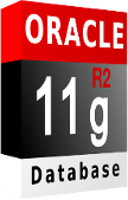
\includegraphics[scale=1]{oracle_11g}}} &
              \multicolumn{1}{c}{\textbf{
\includegraphics[scale=1]{ms_sql}}} &
              \multicolumn{1}{c}{} \\
              \multicolumn{2}{c}{\textbf{Funktionsbezeichnung}} &
              \multicolumn{1}{c}{\textbf{Bedeutung}} \\
              \hline
            }
            \tabletail{
              \hline
            }
            \tablelasttail {
              \hline
            }
            \begin{supertabular}{|c|c|p{11cm}|}
              UPPER & UPPER& Wandelt die gesamte Zeichenkette in Großbuchstaben um.\\
              \hline
              LOWER & LOWER & Wandelt die gesamte Zeichenkette in Kleinbuchstaben um.\\
              \hline
              INITCAP & n. a.& Wandelt das erste Zeichen jedes Wortes in einen Großbuchstaben um.\\
            \end{supertabular}
          \end{small}
        \end{center}
        \begin{merke}
          Die Funktion \languageorasql{INITCAP} existiert in MS SQL Server nicht!
        \end{merke}
\clearpage
        \beispiel{sql03_01} zeigt die Anwendung der drei Funktionen \languageorasql{UPPER}, \languageorasql{LOWER} und \languageorasql{INITCAP} in Oracle.
        \begin{lstlisting}[language=oracle_sql,caption={UPPER, LOWER und INITCAP},label=sql03_01]
SELECT UPPER(Vorname) AS GROSS, LOWER(Nachname) AS Klein,
       INITCAP(Vorname || ' ' || Nachname) AS NORMAL
FROM   Mitarbeiter;
        \end{lstlisting}
        \begin{center}
          \begin{small}
            \changefont{pcr}{m}{n}
            \tablefirsthead {
              \multicolumn{1}{l}{\textbf{GROSS}} &
              \multicolumn{1}{l}{\textbf{KLEIN}} &
              \multicolumn{1}{l}{\textbf{NORMAL}} \\
              \cmidrule(l){1-1}\cmidrule(l){2-2}\cmidrule(l){3-3}
            }
            \tablehead{}
            \tabletail {
            }
            \tablelasttail {
              \multicolumn{3}{l}{\textbf{100 Zeilen ausgewählt}} \\
            }
            \begin{oraclesql}
              \begin{supertabular}{lll}
                MAX & winter & Max Winter \\
                SARAH & werner & Sarah Werner \\
                FINN & seifert & Finn Seifert \\
                SEBASTIAN & schwarz & Sebastian Schwarz \\
              \end{supertabular}
            \end{oraclesql}
          \end{small}
        \end{center}
        \begin{merke}
          Die Anwendung der Funktionen \languageorasql{UPPER} und \languageorasql{LOWER} ist in Oracle und MS SQL Server identisch!
        \end{merke}
        Eingangs wurde erwähnt, das Single Row Functions nicht nur in der \SELECT-Klausel genutzt werden können, sondern, z. B. auch in der \WHERE-Klausel. Dadurch kann das beschriebene Problem der Casesensitivität gelöst werden.
        \begin{lstlisting}[language=oracle_sql,caption={Das Problem der Casesensitivität},label=sql03_02]
SELECT Mitarbeiter_ID, Vorname, Nachname
FROM   Mitarbeiter
WHERE  Nachname LIKE 'winter';
        \end{lstlisting}
        \begin{center}
          \begin{small}
            \changefont{pcr}{m}{n}
            \tablefirsthead {
              \multicolumn{1}{r}{\textbf{MITARBEITER\_ID}} &
              \multicolumn{1}{l}{\textbf{VORNAME}} &
              \multicolumn{1}{l}{\textbf{NACHNAME}} \\
              \cmidrule(r){1-1}\cmidrule(l){2-2}\cmidrule(l){3-3}
            }
            \tablehead{}
            \tabletail {
              \multicolumn{3}{l}{\textbf{Keine Zeilen ausgewählt}} \\
            }
            \tablelasttail {
              \multicolumn{3}{l}{\textbf{Keine Zeilen ausgewählt}} \\
            }
            \begin{oraclesql}
              \begin{supertabular}{rll}

              \end{supertabular}
            \end{oraclesql}
          \end{small}
        \end{center}
        Der Mitarbeiter \enquote{Winter} wird von Oracle nicht gefunden, da er in der Datenbank mit einem großen W am Namensanfang gespeichert ist. Für Oracle sind \enquote{winter} und \enquote{Winter} zwei unterschiedliche Zeichenketten. Hier kann die \languageorasql{LOWER}-Funktion Abhilfe schaffen.
        \begin{lstlisting}[language=oracle_sql,caption={LOWER - Die Lösung des Problems},label=sql03_03]
SELECT Mitarbeiter_ID, Vorname, Nachname
FROM   Mitarbeiter
WHERE  LOWER(Nachname) LIKE 'winter';
        \end{lstlisting}
\clearpage
        \begin{center}
          \begin{small}
            \changefont{pcr}{m}{n}
            \tablefirsthead {
              \multicolumn{1}{r}{\textbf{MITARBEITER\_ID}} &
              \multicolumn{1}{l}{\textbf{VORNAME}} &
              \multicolumn{1}{l}{\textbf{NACHNAME}} \\
              \cmidrule(r){1-1}\cmidrule(l){2-2}\cmidrule(l){3-3}
            }
            \tablehead{}
            \tabletail {
              \multicolumn{3}{l}{\textbf{2 Zeilen ausgewählt}} \\
            }
            \tablelasttail {
              \multicolumn{3}{l}{\textbf{2 Zeilen ausgewählt}} \\
            }
            \begin{oraclesql}
              \begin{supertabular}{rll}
                1 & Max & Winter \\
                9 & Louis & Winter \\
              \end{supertabular}
            \end{oraclesql}
          \end{small}
        \end{center}
        Die \languageorasql{LOWER}-Funktion stellt in \beispiel{sql03_03} sicher, dass alle Werte der Spalte \identifier{Nachname} in Kleinbuchstaben ausgegeben werden. Somit ist der Vergleich mit \enquote{winter} unproblematisch.
      \subsection{Zeichenketten bearbeiten}
        Eine weitere Anwendung von Zeichenkettenfunktionen besteht darin, Teile aus Zeichenketten herauszutrennen oder deren Länge festzustellen. Hierzu kennen Oracle und SQL Server unterschiedliche Funktionen, die in \tabelle{srfstringfct2} beschrieben werden. Sie stellt jedoch nur einen Ausschnitt aus der Menge der Zeichenkettenfunktionen dar.
        \begin{center}
          \tablecaption{Zeichenkettenfunktionen}
          \label{srfstringfct2}
          \begin{small}
            \tablefirsthead{
              \multicolumn{1}{c}{\textbf{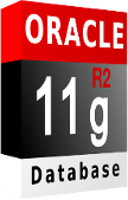
\includegraphics[scale=1]{oracle_11g}}} &
              \multicolumn{1}{c}{\textbf{
\includegraphics[scale=1]{ms_sql}}} &
              \multicolumn{1}{c}{} \\
              \multicolumn{2}{c}{\textbf{Funktionsbezeichnung}} &
              \multicolumn{1}{c}{\textbf{Bedeutung}} \\
              \hline
            }
            \tabletail{
              \hline
            }
            \tablelasttail {
              \hline
            }
            \begin{supertabular}{|l|l|p{10cm}|}
              SUBSTR & SUBSTRING &  Schneidet einen Teil einer Zeichenkette aus und liefert ihn zurück. \\
              \hline
              LENGTH & LEN &  Gibt die Länge einer Zeichenkette zurück. \\
              \hline
              INSTR & CHARINDEX & Diese Funktionen suchen nach Zeichenkette A in
              einer Zeichenkette B und liefern die Position von A zurück. Ist
              A nicht in B erhält man 0 als Ergebnis. \\
            \end{supertabular}
          \end{small}
        \end{center}
        \subsubsection{SUBSTR, LENGTH und INSTR in Oracle}
          Die Funktion \languageorasql{LENGTH} ermittelt, aus wie vielen Zeichen
          ein String besteht. Sie wird meist in Zusammenhang mit den beiden
          anderen Funktionen \languageorasql{SUBSTR} und \languageorasql{INSTR}
          genutzt. \beispiel{sql03_04} zeigt die Anwendung von
          \languageorasql{LENGTH} auf sehr einfache Art und Weise.
          \begin{lstlisting}[language=oracle_sql,caption={Die \languageorasql{LENGTH}-Funktion},label=sql03_04]
SELECT LENGTH(IBAN), IBAN
FROM   Konto
WHERE  Konto_ID = 1281;
          \end{lstlisting}
          \begin{center}
            \begin{small}
              \changefont{pcr}{m}{n}
              \tablefirsthead {
                \multicolumn{1}{r}{\textbf{LENGTH(IBAN)}} &
                \multicolumn{1}{l}{\textbf{IBAN}} \\
                \cmidrule(r){1-1}\cmidrule(l){2-2}
              }
              \tablehead{}
              \tabletail {
%                 \multicolumn{2}{l}{\textbf{1 Zeile ausgewählt}} \\
              }
              \tablelasttail {
                \multicolumn{2}{l}{\textbf{1 Zeile ausgewählt}} \\
              }
              \begin{oraclesql}
                \begin{supertabular}{rl}
                  22 & DE23465387306148533897 \\
                \end{supertabular}
              \end{oraclesql}
            \end{small}
          \end{center}
          Alleine für sich, ist die Information \enquote{22} auf den ersten Blick nutzlos, wenn man aber bedenkt, dass z. B. eine IBAN eine feste Länge von 22 Zeichen hat, kann man mit Hilfe von \languageorasql{LENGTH} verifizieren, ob es sich um eine IBAN mit
          gültiger Länge handelt.

          \languageorasql{SUBSTR} ist dabei behilflich, einen Teil aus einer Zeichenkette auszuschneiden. Eine solche Vorgehensweise ist z. B. dann notwendig, wenn eine Information, in der Form \enquote{Winter, Max}, in einer Tabellenspalte abgelegt ist oder, wenn wie im Falle der IBAN, mehrere Informationen einfach verkettet wurden (Länderkennung, Prüfziffer, BLZ und KtoNr).

          \begin{merke}
            Das Ergebnis einer solchen Operation wird als \enquote{Teilzeichenkette} oder \enquote{Substring} bezeichnet, wobei \enquote{Substring} die geläufigere Variante darstellt.
          \end{merke}
          \beispiel{sql03_05} zeigt die Anwendung der Funktion \languageorasql{SUBSTR}, um die IBAN eines Kontos in ihre Bestandteile zu zerlegen. Hier kann für den dritten wert der Funktion auch eine andere Funktion mit angegeben werden.
          \begin{lstlisting}[language=oracle_sql,caption={Die Anwendung der Funktion \languageorasql{SUBSTR}},label=sql03_05]
SELECT SUBSTR(IBAN, 1, 2) AS Laenderkuerzel, SUBSTR(IBAN, 5 , 8) AS BLZ,
       SUBSTR(IBAN, 13, LEN(IBAN)) AS KtoNr
FROM   Konto
WHERE  Konto_ID = 1281;
          \end{lstlisting}
          \begin{center}
            \begin{small}
              \changefont{pcr}{m}{n}
              \tablefirsthead {
                \multicolumn{1}{l}{\textbf{LAENDE}} &
                \multicolumn{1}{l}{\textbf{BLZ}} &
                \multicolumn{1}{l}{\textbf{KTONR}} \\
                \cmidrule(l){1-1}\cmidrule(l){2-2}\cmidrule(l){3-3}
              }
              \tablehead{}
              \tabletail {
                \multicolumn{2}{l}{\textbf{1 Zeile ausgewählt}} \\
              }
              \tablelasttail {
                \multicolumn{2}{l}{\textbf{1 Zeile ausgewählt}} \\
              }
              \begin{oraclesql}
                \begin{supertabular}{lrr}
                  DE & 46538730 & 6148533897 \\
                \end{supertabular}
              \end{oraclesql}
            \end{small}
          \end{center}
          \begin{center}
            \tablecaption{Funktionsargumente von SUBSTR}
            \label{argsubstr}
            \begin{small}
              \tablefirsthead{
                \multicolumn{1}{c}{\textbf{Argument}} &
                \multicolumn{1}{c}{\textbf{Beispiel}} &
                \multicolumn{1}{c}{\textbf{Erläuterung}} \\
                \hline
              }
              \tablehead{}
              \tabletail{
                \hline
              }
              \tablelasttail{
                \hline
              }
              \begin{supertabular}{|l|c|p{8.5cm}|}
                1 & IBAN &
                Beliebige Zeichenkette (Literal, Spaltenbezeichner oder eine
                andere Funktion). \\
                \hline
                2 & 11 & An welcher Stelle im ersten Argument soll das
                Ausschneiden begonnen werden?. Hier kann eine beliebige
                Integerzahl stehen, die kleiner ist, als die Gesamtlänge von Argument 1. \\
                \hline
                3 & 16 & Mit dem dritten und letzten Argument wird angegeben,
                wie viele Zeichen ausgeschnitten werden sollen.
                \begin{itemize}
                  \item n > 1: Es werden n Zeichen ausgeschnitten.
                  \item n nicht angegeben: Es werden alle Zeichen, bis zum Ende der Zeichenkette angezeigt.
                  \item n < 1: NULL-Wert als Ergebnis
                \end{itemize} \\
              \end{supertabular}
            \end{small}
          \end{center}

          Mit \languageorasql{INSTR} kann die Position eines Zeichens oder einer
          Zeichenkette in einer Zeichenkette bestimmt werden. Eine typische
          Aufgabenstellung könnte sein: \enquote{Bestimme ob das
          Länderkürzel DE in der IBAN vorkommt}.
          In SQL ausgedrückt sieht dies so aus:
          \begin{lstlisting}[language=oracle_sql,caption={Automatische Positionsbestimmung},label=sql03_06]
SELECT INSTR(IBAN, 'DE') AS Position
FROM   Konto
WHERE  Konto_ID = 1281;
          \end{lstlisting}
          \begin{center}
            \begin{small}
              \changefont{pcr}{m}{n}
              \tablefirsthead {
                \multicolumn{1}{r}{\textbf{POSITION}} \\
                \cmidrule(r){1-1}
              }
              \tablehead{}
              \tabletail {
                \multicolumn{1}{l}{\textbf{1 Zeile ausgewählt}} \\
              }
              \tablelasttail {
                \multicolumn{1}{l}{\textbf{1 Zeile ausgewählt}} \\
              }
              \begin{oraclesql}
                \begin{supertabular}{r}
                  1 \\
                \end{supertabular}
              \end{oraclesql}
            \end{small}
          \end{center}
          \beispiel{sql03_06} zeigt, wie mit Hilfe der
          \languageorasql{INSTR}-Funktion die Position eines einzelnen Zeichens
          bzw. mehrere Zeichen in einer Zeichenkette ermittelt werden kann.
          \begin{center}
            \tablecaption{Funktionsargumente von INSTR}
            \label{arginstr}
            \begin{small}
              \tablefirsthead{
                \multicolumn{1}{c}{\textbf{Argument}} &
                \multicolumn{1}{c}{\textbf{Beispiel}} &
                \multicolumn{1}{c}{\textbf{Erläuterung}} \\
                \hline
              }
              \tablehead{}
              \tabletail{
                \hline
              }
              \tablelasttail{
                \hline
              }
              \begin{supertabular}{|l|c|p{8.5cm}|}
                1 & IBAN &
                Beliebige Zeichenkette (Literal, Spaltenbezeichner oder eine
                andere Funktion). \\
                \hline
                2 & 'DE' & Das zweite Argument gibt an, nach welchem Zeichen /
                welcher Zeichenkette gesucht werden soll. \\
              \end{supertabular}
            \end{small}
          \end{center}
          \begin{merke}
            Die Funktion \languageorasql{INSTR} kennt noch zwei weitere
            Parameter, welche hier nicht näher erläutert werden. Weitere
            Informationen zu dieser Funktion können aus der
            Online-Dokumentation entnommen werden.
          \end{merke}
          Die folgenden Links verweisen auf die Online-Dokumentation der
          Oracle-Datenbank.
          \begin{literaturinternet}
            \item \cite{i77725}
            \item \cite{i87066}
            \item \cite{i77598}
          \end{literaturinternet}
\clearpage
        \subsubsection{SUBSTRING, LEN und CHARINDEX in MS SQL Server}
          Die Funktion \languagemssql{LEN} ermittelt, aus wie vielen Zeichen ein
          String besteht. Sie wird meist in Zusammenhang mit den beiden anderen
          Funktionen \languagemssql{SUBSTRING} und \languagemssql{CHARINDEX}
          genutzt. \beispiel{sql03_08} zeigt die Anwendung von
         \languagemssql{LEN} auf sehr einfache Art und Weise.
          \begin{lstlisting}[language=ms_sql,caption={Die \languagemssql{LEN}-Funktion},label=sql03_08]
SELECT LEN(IBAN), IBAN
FROM   Konto
WHERE  Konto_ID = 1281;
          \end{lstlisting}
          \begin{center}
            \begin{small}
              \changefont{pcr}{m}{n}
              \tablefirsthead {
                \multicolumn{1}{l}{\textbf{(Kein Spaltenname)}} &
                \multicolumn{1}{l}{\textbf{Nachname}} \\
                \cmidrule(l){1-1}\cmidrule(l){2-2}
              }
              \tablehead{}
              \tabletail {
                \multicolumn{2}{l}{\textbf{1 Zeile ausgewählt}} \\
              }
              \tablelasttail {
                \multicolumn{2}{l}{\textbf{1 Zeile ausgewählt}} \\
              }
              \begin{mssql}
                \begin{supertabular}{ll}
                  22 & DE23465387306148533897 \\
                \end{supertabular}
              \end{mssql}
            \end{small}
          \end{center}
          Alleine für sich, ist die Information \enquote{22} auf den
          ersten Blick nutzlos, wenn man aber bedenkt, dass z. B. eine IBAN
          eine feste Länge von 22 Zeichen hat, kann man mit Hilfe von
          \languagemssql{LEN} verifizieren, ob es sich um eine IBAN mit
          gültiger Länge handelt.

          \languagemssql{SUBSTRING} ist dabei behilflich, einen Teil aus einer Zeichenkette auszuschneiden. Eine solche Vorgehensweise ist z. B. dann notwendig, wenn eine Information, in der Form \enquote{Winter, Max}, in einer Tabellenspalte abgelegt ist oder, wenn wie im Falle der IBAN, mehrere Informationen einfach verkettet wurden (Länderkennung, Prüfziffer, BLZ und KtoNr).

          \begin{merke}
            Das Ergebnis einer solchen Operation wird als \enquote{Teilzeichenkette} oder \enquote{Substring} bezeichnet, wobei \enquote{Substring} die geläufigere Variante darstellt.
          \end{merke}
          \beispiel{sql03_09} zeigt die Anwendung der Funktion \languagemssql{SUBSTRING}, um die IBAN eines Kontos in ihre Bestandteile zu zerlegen.
          \begin{lstlisting}[language=ms_sql,caption={Die Anwendung der Funktion \languagemssql{SUBSTRING}},label=sql03_09]
SELECT SUBSTRING(IBAN, 1, 2) AS Laenderkuerzel, SUBSTRING(IBAN, 5 , 8) AS BLZ,
       SUBSTRING(IBAN, 14) AS KtoNr
FROM   Konto
WHERE  Konto_ID = 1281;
          \end{lstlisting}
\clearpage
          \begin{center}
            \begin{small}
              \changefont{pcr}{m}{n}
              \tablefirsthead {
                \multicolumn{1}{l}{\textbf{LAENDE}} &
                \multicolumn{1}{l}{\textbf{BLZ}} &
                \multicolumn{1}{l}{\textbf{KTONR}} \\
                \cmidrule(l){1-1}\cmidrule(l){2-2}\cmidrule(l){3-3}
              }
              \tablehead{}
              \tabletail {
                \multicolumn{2}{l}{\textbf{1 Zeile ausgewählt}} \\
              }
              \tablelasttail {
                \multicolumn{2}{l}{\textbf{1 Zeile ausgewählt}} \\
              }
              \begin{mssql}
                \begin{supertabular}{lll}
                  DE & 46538730 & 6148533897 \\
                \end{supertabular}
              \end{mssql}
            \end{small}
          \end{center}
          \begin{center}
            \tablecaption{Funktionsargumente von SUBSTR}
            \label{argSUBSTRING}
            \begin{small}
              \tablefirsthead{
                \multicolumn{1}{c}{\textbf{Argument}} &
                \multicolumn{1}{c}{\textbf{Beispiel}} &
                \multicolumn{1}{c}{\textbf{Erläuterung}} \\
                \hline
              }
              \tablehead{}
              \tabletail{
                \hline
              }
              \tablelasttail{
                \hline
              }
              \begin{supertabular}{|l|c|p{8.5cm}|}
                1 & IBAN &
                Beliebige Zeichenkette (Literal, Spaltenbezeichner oder eine
                andere Funktion). \\
                \hline
                2 & 11 & An welcher Stelle im ersten Argument soll das
                Ausschneiden begonnen werden?. Hier kann eine beliebige
                Integerzahl stehen, die kleiner ist, als die Gesamtlänge von Argument 1. \\
                \hline
                3 & 16 & Mit dem dritten und letzten Argument wird angegeben,
                wie viele Zeichen ausgeschnitten werden sollen.
                \begin{itemize}
                  \item n > 1: Es werden n Zeichen ausgeschnitten.
                  \item n nicht angegeben: Es werden alle Zeichen, bis zum Ende der Zeichenkette angezeigt.
                  \item n < 1: NULL-Wert als Ergebnis
                \end{itemize} \\
              \end{supertabular}
            \end{small}
          \end{center}
          Mit \languagemssql{CHARINDEX} kann die Position eines Zeichens oder
          einer Zeichenkette in einer Zeichenkette bestimmt werden. Eine
          typische Aufgabenstellung könnte sein: \enquote{Bestimme ob das
          Länderkürzel DE in der IBAN vorkommt}. In SQL ausgedrückt sieht dies so aus:
          \begin{lstlisting}[language=ms_sql,caption={Automatische Positionsbestimmung},label=sql03_10]
SELECT CHARINDEX('DE', IBAN) AS Position
FROM   Konto
WHERE  Konto_ID = 1281;
          \end{lstlisting}

          \begin{center}
            \begin{small}
              \changefont{pcr}{m}{n}
              \tablefirsthead {
                \multicolumn{1}{l}{\textbf{POSITION}} \\
                \cmidrule(r){1-1}
              }
              \tablehead{}
              \tabletail {
                \multicolumn{1}{l}{\textbf{1 Zeile ausgewählt}} \\
              }
              \tablelasttail {
                \multicolumn{1}{l}{\textbf{1 Zeile ausgewählt}} \\
              }
              \begin{mssql}
                \begin{supertabular}{l}
                  1 \\
                \end{supertabular}
              \end{mssql}
            \end{small}
          \end{center}
          \beispiel{sql03_10} zeigt, wie mit Hilfe der
          \languagemssql{CHARINDEX}-Funktion die Position eines einzelnen
          Zeichens in einer Zeichenkette ermittelt werden kann.
          \begin{center}
            \tablecaption{Funktionsargumente von CHARINDEX}
            \label{argcharindex}
            \begin{small}
              \tablefirsthead{
                \multicolumn{1}{c}{\textbf{Argument}} &
                \multicolumn{1}{c}{\textbf{Beispiel}} &
                \multicolumn{1}{c}{\textbf{Erläuterung}} \\
                \hline
              }
              \tablehead{}
              \tabletail{
                \hline
              }
              \tablelasttail{
                \hline
              }
              \begin{supertabular}{|l|c|p{8.5cm}|}
                1 & 'DE' & Das erste Argument gibt an, nach welchem Zeichen /
                welcher Zeichenkette gesucht werden soll. \\
                \hline
                2 & Nachname + ', ' + Vorname & Das zwei Argument ist eine
                beliebige Zeichenkette. An dieser Stelle kann ein Literal, ein
                Spaltenbezeichner oder eine andere Funktion stehen. \\
                \hline
              \end{supertabular}
            \end{small}
          \end{center}
          \begin{merke}
            Die Funktion \languagemssql{CHARINDEX} kennt noch einen weiteren
            Parameter, welcher hier nicht näher erläutert wird. Weitere
            Informationen zu dieser Funktion können aus der
            Online-Dokumentation, der MSDN, entnommen werden.
          \end{merke}
          Die folgenden Links verweisen auf die Online-Dokumentation des MS SQL
          Server, im Microsoft Developer Network (MSDN).
          \begin{literaturinternet}
            \item \cite{ms190329}
            \item \cite{ms187748}
            \item \cite{ms186323}
          \end{literaturinternet}
    \section{Arithmetische Funktionen}
      Arithmetische Funktionen dienen dazu Berechnungen anzustellen. Dies kann
      beispielsweise sein:
      \begin{itemize}
        \item Runden,
        \item Radizieren (Wurzelziehen),
        \item Potenzieren,
        \item Logarithmieren
      \end{itemize}
      und vieles mehr. In dieser Unterrichtsunterlage werden nur einige
      Beispiele gezeigt.
      \subsection{FROM oder nicht FROM, das ist hier die Frage}
        In \beispiel{sql03_12} und \beispiel{sql03_13} wird die Berechnung der
        Quadratwurzel, der Zahl 4, in Oracle und MS SQL Server gezeigt. Die
        Anwendung der Funktion \languageorasql{SQRT} ist in beiden Systemen
        gleich. Trotztdem existiert ein gravierender Unterschied zwischen beiden
        Beispielen.
        \begin{lstlisting}[language=oracle_sql,caption={Berechnung der Quadartwurzel, der Zahl 4, in Oracle},label=sql03_12]
SELECT SQRT(4) AS "Wurzel 4"
FROM   dual;
        \end{lstlisting}
\clearpage
        \begin{lstlisting}[language=ms_sql,caption={Berechnung der Quadratwurzel, der Zahl 4, in MS SQL Server},label=sql03_13]
SELECT SQRT(4) As "Wurzel 4";
        \end{lstlisting}
        \begin{center}
          \begin{small}
            \changefont{pcr}{m}{n}
            \tablefirsthead {
              \multicolumn{1}{r}{\textbf{Wurzel 4}} \\
              \cmidrule(r){1-1}
            }
            \tablehead{}
            \tabletail {
              \multicolumn{1}{l}{\textbf{1 Zeile ausgewählt}} \\
            }
            \tablelasttail {
              \multicolumn{1}{l}{\textbf{1 Zeile ausgewählt}} \\
            }
            \begin{msoraclesql}
              \begin{supertabular}{r}
                2 \\
              \end{supertabular}
            \end{msoraclesql}
          \end{small}
        \end{center}
        Eingangs wurde behauptet, dass jedes \SELECT-Statement immer eine
        \FROM-Klausel benötigen würde. Dies ist gemäß SQL-Standard
        auch richtig. Das DBMS Oracle setzt an dieser Stelle den Standard
        konsequent um, der MS SQL Server nicht.

        \begin{merke}
          Im DBMS Oracle muss jedes \SELECT-Statement immer eine \FROM-Klausel
          aufweisen, in MS SQL Server nicht.
        \end{merke}
			 Um den SQL-Standard einhalten zu können, gibt es in Oracle eine \enquote{Dummy-Tabelle} namens \identifier{dual}. Diese enthält nur eine 		 Spalte, mit einer Zeile, wie in \beispiel{sql03_14} zu sehen ist. Sie kommt immer dann zum Einsatz, wenn das Ergebnis einer Funktion, unabhängig von irgendwelchen Datensätzen, abgerufen werden muss.
        \begin{lstlisting}[language=oracle_sql,caption={Die Tabelle \identifier{dual} in Oracle},label=sql03_14]
SELECT *
FROM   dual;
        \end{lstlisting}
        \begin{center}
          \begin{small}
            \changefont{pcr}{m}{n}
            \tablefirsthead {
              \multicolumn{1}{l}{\textbf{DUMMY}} \\
              \cmidrule(l){1-1}
            }
            \tablehead{}
            \tabletail {
              \multicolumn{1}{l}{\textbf{1 Zeile ausgewählt}} \\
            }
            \tablelasttail {
              \multicolumn{1}{l}{\textbf{1 Zeile ausgewählt}} \\
            }
            \begin{oraclesql}
              \begin{supertabular}{l}
                X \\
              \end{supertabular}
            \end{oraclesql}
          \end{small}
        \end{center}
        Der MS SQL Server kommt ohne diese Tabelle aus, da bei ihm die
        \FROM-Klausel einfach weggelassen werden darf.
      \subsection{Arithmetische Funktionen anwenden}
        Oracle kennt ca. 30 und MS SQL Server ca. 20 arithmetische Funktionen.
        Ziel dieser Unterrichtsunterlage ist es, einige wenige davon
        herauszugreifen und deren Anwendung zu erläutern. Hierbei handelt es
        sich um die folgenden Funktionen:
\clearpage
        \begin{center}
          \tablecaption{Arithmetische Funktionen}
          \label{srfarithmfct}
          \begin{small}
            \tablefirsthead{
              \multicolumn{1}{c}{\textbf{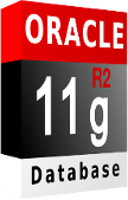
\includegraphics[scale=1]{oracle_11g}}} &
              \multicolumn{1}{c}{\textbf{
\includegraphics[scale=1]{ms_sql}}} &
              \multicolumn{1}{c}{} \\
              \multicolumn{2}{c}{\textbf{Funktionsbezeichnung}} &
              \multicolumn{1}{c}{\textbf{Bedeutung}} \\
              \hline
            }
            \tabletail{
              \hline
            }
            \tablelasttail {
              \hline
            }
            \begin{supertabular}{|l|l|p{10cm}|}
              CEIL & CEILING & Gibt immer die kleinste ganze Zahl aus, die
              größer oder gleich n ist (Ganzzahliges Aufrunden).\\
              \hline
              FLOOR & FLOOR & Gibt immer die größte ganze Zahl aus, die
              kleiner oder gleich n ist (Ganzzahliges Abrunden). \\
              \hline
              LOG & LOG 10 & Berechnet den Logarithmus der Zahl x zur Basis n. MS-SQL nur zur Basis 10 \\
              \hline
              MOD & \% & Gibt den Rest einer ganzzahligen Division zurück. \\
              \hline
              POWER & POWER & Potenziert die Zahl x mit n. \\
              \hline
              ROUND & ROUND & Auf- bzw. Abrunden einer Zahl nach dem
              kaufmännischen Rundungsverfahren ($x < 0,5$ = Abrunden, $x \geqq
              0,5$ = Aufrunden). \\
              \hline
              TRUNC & n. a. & Schneidet die Nachkommastellen einer Zahl ab und
              gibt den ganzzahligen Anteil zurück. \\
            \end{supertabular}
          \end{small}
        \end{center}
        In den beiden folgenden Beispielen wird die Anwendung von
        Rundungsfunktionen in Oracle und MS SQL Server gezeigt.
        \begin{lstlisting}[language=oracle_sql,caption={Rundungsfunktionen in Oracle},label=sql03_15]
SELECT SQRT(3) AS "Wurzel 3", CEIL(SQRT(3)) AS "Aufrunden",
       FLOOR(SQRT(3)) AS "Abrunden",
       ROUND(SQRT(3), 2) AS "Kaufm. runden"
FROM   dual;
        \end{lstlisting}
        \begin{center}
          \begin{small}
            \changefont{pcr}{m}{n}
            \tablefirsthead {
              \multicolumn{1}{r}{\textbf{Wurzel 3}} &
              \multicolumn{1}{r}{\textbf{Aufrunden}} &
              \multicolumn{1}{r}{\textbf{Abrunden}} &
              \multicolumn{1}{r}{\textbf{Kaufm. runden}} \\
              \cmidrule(r){1-1}\cmidrule(r){2-2}\cmidrule(r){3-3}\cmidrule(r){4-4}
            }
            \tablehead{}
            \tabletail {
              \multicolumn{4}{l}{\textbf{1 Zeile ausgewählt}} \\
            }
            \tablelasttail {
              \multicolumn{4}{l}{\textbf{1 Zeile ausgewählt}} \\
            }
            \begin{oraclesql}
              \begin{supertabular}{rrrr}
                1,7320508 & 2 & 1 & 1,73 \\
              \end{supertabular}
            \end{oraclesql}
          \end{small}
        \end{center}
        Die Funktionen aus \beispiel{sql03_15} sind weitestgehend
        selbsterklärend. Die mit \languageorasql{SQRT(3)} erzeugte Zahl
        1,7320508 wird durch \languageorasql{CEIL} aufgerundet auf 2, von
        \languageorasql{FLOOR} abgerundet auf 1 und mit Hilfe von
        \languageorasql{ROUND} kaufmännisch, auf zwei Nachkommastellen,
        aufgerundet.

        \begin{merke}
          Die Funktion \languageorasql{ROUND} rundet kaufmännisch. Das zweite
          Argument gibt an, auf welche Nachkommastelle gerundet werden soll.
          Durch die Angabe von 0 wird auf die nächste ganze Zahl gerundet.
        \end{merke}
        Die Anwendung dieser Funktionen ist im MS SQL Server identisch, mit der
        Ausnahme das \languageorasql{CEIL} dort \languagemssql{CEILING}
        heißt.
\clearpage
        \begin{lstlisting}[language=ms_sql,caption={Rundungsfunktionen in MS SQL},label=sql03_16]
SELECT SQRT(3) AS "Wurzel 3", CEILING(SQRT(3)) AS "Aufrunden",
       FLOOR(SQRT(3)) AS "Abrunden",
       ROUND(SQRT(3), 2) AS "Kaufm. runden";
        \end{lstlisting}
        \begin{center}
          \begin{small}
            \changefont{pcr}{m}{n}
            \tablefirsthead {
              \multicolumn{1}{l}{\textbf{Wurzel 3}} &
              \multicolumn{1}{l}{\textbf{Aufrunden}} &
              \multicolumn{1}{l}{\textbf{Abrunden}} &
              \multicolumn{1}{l}{\textbf{Kaufm. runden}} \\
              \cmidrule(l){1-1}\cmidrule(l){2-2}\cmidrule(l){3-3}\cmidrule(l){4-4}
            }
            \tablehead{}
            \tabletail {
              \multicolumn{4}{l}{\textbf{1 Zeile ausgewählt}} \\
            }
            \tablelasttail {
              \multicolumn{4}{l}{\textbf{1 Zeile ausgewählt}} \\
            }

            \begin{mssql}
              \begin{supertabular}{llll}
                1,7320508 & 2 & 1 & 1,73 \\
              \end{supertabular}
            \end{mssql}
          \end{small}
        \end{center}
        In \beispiel{sql03_15} bzw. \beispiel{sql03_16} ist zu sehen, dass es
        möglich ist, Funktionen in einander zu verschachteln. Mit Hilfe des
        Ausdrucks \languageorasql{SQRT(3)} wird die Quadratwurzel der Zahl 3
        errechnet (1,73205080756888). Dieser Wert soll anschließend auf 2
        Nachkommastellen gerundet werden. Hierzu kann auf beiden Systemen die
        Funktion \languageorasql{ROUND} herangezogen werden. 
        
        Bei der Abarbeitung des Ausdrucks \languageorasql{ROUND(SQRT(3),2)}
        halten sich Oracle und SQL Server an die Gesetze der Arithmetik, d. h.
        es wird zuerst der innerste Ausdruck (in diesem Falle
        \languageorasql{SQRT(3)}) aufgelöst und anschließend wird das
        Ergebnis dieses Ausdrucks durch die Funktion \languageorasql{ROUND} auf
        zwei Nachkommastellen gerundet.

        Die zweite Gruppe der arithmetischen Funktionen, die hier vorgestellt
        werden sollen, bilden die sogenannten \enquote{höhreren Rechenarten}
        ab. Dies sind: Radizieren, Potenzieren, Logarithmieren. Zusätzlich ist
        hier noch die Modulo-Operation dargestellt, die den Rest einer
        ganzzahlingen Divison ausgibt.
        \begin{lstlisting}[language=oracle_sql,caption={Höhere Rechenarten in Oracle},label=sql03_17]
SELECT MOD(9, 2) AS Modulo, POWER(10, 2) AS Power,
       LOG(10, 1000) AS Log, SQRT(16) AS Quadratwurzel,
       SQRT(27) / SQRT(3) AS "3. Wurzel von 27",
       LOG(5, 8) AS "Log 8 Basis 5"
FROM   dual;
        \end{lstlisting}
        \begin{center}
          \begin{small}
            \changefont{pcr}{m}{n}
            \tablefirsthead {
              \multicolumn{1}{r}{\textbf{Modulo}} &
              \multicolumn{1}{r}{\textbf{Power}} &
              \multicolumn{1}{r}{\textbf{Log}} &
              \multicolumn{1}{r}{\textbf{Quadratwurzel}} &
              \multicolumn{1}{r}{\textbf{3. Wurzel von 27}} &
              \multicolumn{1}{r}{\textbf{Log 8 Basis 5}} \\
              \cmidrule(r){1-1}\cmidrule(r){2-2}\cmidrule(r){3-3}\cmidrule(r){4-4}\cmidrule(r){5-5}
              \cmidrule(r){6-6}
            }
            \tablehead{}
            \tabletail {
              \multicolumn{6}{l}{\textbf{1 Zeile ausgewählt}} \\
            }
            \tablelasttail {
              \multicolumn{6}{l}{\textbf{1 Zeile ausgewählt}} \\
            }
            \begin{oraclesql}
              \begin{supertabular}{rrrrrr}
                1 & 100 & 3 & 4 & 3 & 1,292029 \\
              \end{supertabular}
            \end{oraclesql}
          \end{small}
        \end{center}
        In MS SQL Server können die gleichen Berechnungen durchgeführt
        werden, jedoch mit dem Unterschied, dass:
        \begin{itemize}
          \item Die Modulo-Operation durch den \%-Operator dargestellt wird und
          nicht durch eine Funktion.
          \item Es gibt in MS SQL Server keine Entsprechung zur
          \languageorasql{LOG}-Funktion.
        \end{itemize}
        In MS SQL Server gibt es nur die Funktion \languagemssql{LOG10}
        (Dekadischer Logarithmus zur Basis 10). Um nun die
        \languageorasql{LOG}-Funktion von Oracle nachzustellen muss hier $log_58
        = log_{10}8 / log_{10}5$ gerechnet werden.
        \begin{lstlisting}[language=ms_sql,caption={Höhere Rechenarten in MS SQL Server},label=sql03_18]
SELECT 9 % 2 AS Modulo, POWER(10, 2) AS Power,
       LOG10(1000) AS Log, SQRT(16) AS Quadratwurzel,
       SQRT(27) / SQRT(3) AS "3. Wurzel von 27",
       LOG10(8) / LOG10(5) AS "Log 8 Basis 5";
        \end{lstlisting}
        \begin{center}
          \begin{small}
            \changefont{pcr}{m}{n}
            \tablefirsthead {
              \multicolumn{1}{l}{\textbf{Modulo}} &
              \multicolumn{1}{l}{\textbf{Power}} &
              \multicolumn{1}{l}{\textbf{Log}} &
              \multicolumn{1}{l}{\textbf{Quadratwurzel}} &
              \multicolumn{1}{l}{\textbf{3. Wurzel von 27}} &
              \multicolumn{1}{l}{\textbf{Log 8 Basis 5}} \\
              \cmidrule(l){1-1}\cmidrule(l){2-2}\cmidrule(l){3-3}\cmidrule(l){4-4}\cmidrule(l){5-5}
              \cmidrule(l){6-6}
            }
            \tablehead{}
            \tabletail {
              \multicolumn{6}{l}{\textbf{1 Zeile ausgewählt}} \\
            }
            \tablelasttail {
              \multicolumn{6}{l}{\textbf{1 Zeile ausgewählt}} \\
            }
            \begin{mssql}
              \begin{supertabular}{llllll}
                1 & 100 & 3 & 4 & 3 & 1,292029 \\
              \end{supertabular}
            \end{mssql}
          \end{small}
        \end{center}
        \begin{literaturinternet}
          \item \cite{i97801}
          \item \cite{i77449}
          \item \cite{i84140}
          \item \cite{i77996}
          \item \cite{i78493}
          \item \cite{i78633}
          \item \cite{ms189818}
          \item \cite{ms178531}
          \item \cite{ms175121}
          \item \cite{ms174276}
          \item \cite{ms175003}
        \end{literaturinternet}
    \section{Datumsfunktionen}
      \subsection{Datumswerte}
        Der Umgang mit Datumswerten in einer Datenbank ist meist nicht einfach.
        Jedes RDBMS speichert Datumsangaben anders und behandelt diese auch
        anders. Aus diesem Grund soll an dieser Stelle erst einmal ein
        Überblick darüber gegeben werden, wie Oracle und MS SQL Server mit
        Datumswerten umgehen.
 \clearpage
        \begin{center}
          \tablecaption{Behandlung von Datumswerten}
          \label{datevalues}
          \begin{small}
            \tablefirsthead{
              \multicolumn{1}{c}{\textbf{Eigenschaft}} &
              \multicolumn{1}{c}{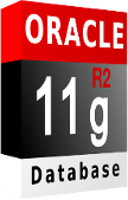
\includegraphics[scale=1]{oracle_11g}} &
              \multicolumn{1}{c}{
\includegraphics[scale=1]{ms_sql}} \\
              \hline
            }
            \tabletail{
              \hline
            }
            \tablelasttail{
              \hline
            }
            \begin{supertabular}{|l|p{5.5cm}|p{5.35cm}|}
              Standarddatumsformat & DD-MON-YY (z. B. 12-NOV-08) & yyyy-mm-ddThh:mm:ss[.mmm] (z. B.  2004-05-23T14:25:10.487) \\
              \hline
              Speicherung & internes numerisches Format & internes numerisches Format \\
              \hline
              Wertebereich & Von 4713 vor Christus bis Dezember 9999. & Zwischen dem 1. Januar 1753 und dem 31. Dezember 9999. \\
              \hline
              Systemdatum anzeigen & SYSDATE / SYSTIMESTAMP & getdate() \\
            \end{supertabular}
          \end{small}
        \end{center}
      \subsection{Datumsarithmetik in Oracle}
        Unter dem Begriff \enquote{Datumsarithmetik} versteht man das Rechnen mit Datumswerten. In Oracle gibt es zwei Möglichkeiten:
        \begin{itemize}
          \item Addition oder Subtraktion von Zahlen zu einem Datumswert
          \item Verwendung von Interval-Literalen
        \end{itemize}
        Führt man Datumsarithmetik durch Addition oder Subtraktion von Zahlen durch gelten folgende Regeln:
        \begin{itemize}
          \item Ganze Zahlen sind Tage, z. B. 1 ist ein Tag, 15 sind fünfzehn Tage
          \item Fraktale (Nachkommastellen) sind Stunden, Minuten und Sekunden, z. B. $\frac{1}{24}=0,041666$ ist eine Stunde oder $\frac{\frac{1}{24}}{60}=0,000694444$ ist eine Minute
          \item Es darf nur addiert oder subtrahiert werden, alle anderen Rechenoperationen sind verboten.
        \end{itemize}
        Einige Beispiele hierzu: So oder in Kommandozeile SQLPLUS !
      
        \begin{lstlisting}[language=oracle_sql,caption={Einfache Datumsarithmetik in Oracle},label=sql03_19]
SELECT to_char (SYSDATE,'DD.MM.yyyyhh24:mm:ss) AS "Datum/Uhrzeit", SYSDATE + 2 AS "2 Tage",
       to_char (SYSDATE - 3 / 24,'DD.MM.yyyyhh24:mm:ss) AS "3 Stunden"
FROM   dual;
        \end{lstlisting}
        \begin{center}
          \begin{small}
            \changefont{pcr}{m}{n}
            \tablefirsthead {
              \multicolumn{1}{l}{\textbf{Datum/Uhrzeit}} &
              \multicolumn{1}{l}{\textbf{2 Tage}} &
              \multicolumn{1}{l}{\textbf{3 Stunden}} \\
              \cmidrule(l){1-1}\cmidrule(l){2-2}\cmidrule(l){3-3}
            }
            \tablehead{}
            \tabletail {
%               \multicolumn{3}{l}{\textbf{1 Zeile ausgewählt}} \\
            }
            \tablelasttail {
              \multicolumn{3}{l}{\textbf{1 Zeile ausgewählt}} \\
            }
            \begin{oraclesql}
              \begin{supertabular}{lll}
                30.04.2013 14:36:24 & 02.05.2013 14:36:24 & 30.04.2013 11:36:24 \\
              \end{supertabular}
            \end{oraclesql}
          \end{small}
        \end{center}
        \subsubsection{Intervall-Literale (Oracle)}
          Intervall-Literale sind dazu da, um Zeiträume anzugeben. Diese
          können in Form von Jahren, Monaten, Tagen, Stunden, Minuten oder
          Sekunden ausgedrückt werden. Es gibt zwei grundsätzlich 
          unterschiedliche Arten von Intervallen:
          \begin{itemize}
            \item YEAR TO MONTH
            \item DAY TO SECOND
          \end{itemize}
          Das YEAR TO MONTH Intervall kann aus bis zu zwei Feldern bestehen,
           wobei das erste die Jahre und das zweite die Monate angibt.
           \tabelle{yeartomonth} zeigt hierzu einige Beispiele.
          \begin{center}
            \tablecaption{Das YEAR TO MONTH Intervall}
            \label{yeartomonth}
            \begin{small}
              \tablefirsthead{
                \multicolumn{1}{c}{\textbf{Beispiel}} &
                \multicolumn{1}{c}{\textbf{Bedeutung}} \\
                \hline
              }
              \tabletail{
                \hline
              }
              \tablelasttail{
                \hline
              }
              \begin{supertabular}{|l|p{9cm}|}
                \texttt{INTERVAL '10' YEAR} & Ein Intervall von 10 Jahren (und 0 Monaten) \\
                \hline
                \texttt{INTERVAL '101' YEAR(3)} & Ein Intervall von 101 Jahren \\
                \hline
                \texttt{INTERVAL '10' YEAR TO YEAR} & Das gleiche wie \texttt{INTERVAL '10' YEAR} \\
                \hline
                \texttt{INTERVAL '10-3' YEAR TO MONTH} & Ein Intervall von 10 Jahren und 3 Monaten \\
                \hline
                \texttt{INTERVAL '27' MONTH} & Ein Intervall von 27 Monaten \\
              \end{supertabular}
            \end{small}
          \end{center}
           Bei der Angabe von Intervall-Literalen gibt es wichtige Dinge zu
           beachten:
          \begin{itemize}
            \item Die Zeitangabe wird immer in Hochkommas gesetzt,
            \item zu jedem Intervall muss angegeben werden, ob es sich um Jahre (YEAR) oder Monate (MONTH) handelt,
            \item die Standardpräzision eines YEAR TO MONTH Intervalls ist immer 2-stellig. Bei drei- oder mehrstelligen Jahresangaben, muss die Präzision angegeben werden. In \beispiel{sql03_20} wird dieses Problem gezeigt.
          \end{itemize}
          \begin{lstlisting}[language=oracle_sql,caption={Richtiger Umgang mit YEAR TO MONTH Intervallen},label=sql03_20]
SELECT SYSDATE - INTERVAL '101' YEAR
FROM   dual;

ORA-01873: the leading precision of the interval is too small 
01873. 00000 -  "the leading precision of the interval is too small"
*Cause:    The leading precision of the interval is too small to store the
           specified interval.
*Action:   Increase the leading precision of the interval or specify an
           interval with a smaller leading precision.

SELECT SYSDATE - INTERVAL '101' YEAR(3)
FROM   dual;
          \end{lstlisting}
\clearpage
          \begin{center}
            \begin{small}
              \changefont{pcr}{m}{n}
              \tablefirsthead {
                \multicolumn{1}{l}{\textbf{SYSDATE-INTERVAL'101(3)'YEAR}} \\
                \cmidrule(l){1-1}
              }
              \tablehead{}
              \tabletail {
                \multicolumn{1}{l}{\textbf{1 Zeile ausgewählt}} \\
              }
              \tablelasttail {
                \multicolumn{1}{l}{\textbf{1 Zeile ausgewählt}} \\
              }
              \begin{oraclesql}
                \begin{supertabular}{l}
                  02.05.03 \\
                \end{supertabular}
              \end{oraclesql}
            \end{small}
          \end{center}
          \begin{merke}
            Mit der Präzision wird angegeben, wie viele Stellen die
            Jahresangabe haben darf. Der Standardwert ist 2.
          \end{merke}
          \beispiel{sql03_20} zeigt, dass die Angaben \languageorasql{INTERVAL
          '101' YEAR} mit dem Oracle-Fehler ORA-01873 scheitert, da die
          Standardpräzision nur 2-stellig ist und daher bei einer
          dreistelligen Jahresangabe die Präzision durch die Angaben
          \languageorasql{YEAR(3)} auf drei Stellen erhöht werden muss.

          Bei der zweiten Art von Intervall-Literal, dem DAY TO SECOND Intervall
          verhält es sich mit der Syntax genauso, wie beim YEAR TO MONTH
          Intervall. \tabelle{daytosecond} zeigt Beispiele für solche
          Intervalle.
          \begin{center}
            \tablecaption{Das DAY TO SECOND Intervall}
            \label{daytosecond}
            \begin{small}
              \tablefirsthead{
                \multicolumn{1}{c}{\textbf{Beispiel}} &
                \multicolumn{1}{c}{\textbf{Bedeutung}} \\
                \hline
              }
              \tabletail{
                \hline
              }
              \tablelasttail{
                \hline
              }
              \begin{supertabular}{|l|p{8.8cm}|}
                \texttt{INTERVAL '8' DAY} & Ein Intervall von 8 Tagen \\
                \hline
                \texttt{INTERVAL '8 4' DAY TO HOUR} & Ein Intervall von 8 Tagen und 4 Stunden \\
                \hline
                \texttt{INTERVAL '8 4:25' DAY TO MINUTE} & Ein Intervall von 8 Tagen, 4 Stunden und 25 Minuten \\
                \hline
                \texttt{INTERVAL '8 4:25:10' DAY TO SECOND} & 8 Tage, 4 Stunden, 25 Minuten und 10 Sekunden \\
                \hline
                \texttt{INTERVAL '120' DAY(3)} & 120 Tage (Präzision 3!!!) \\
                \hline
                \texttt{INTERVAL '3' HOUR} & 3 Stunden \\
                \hline
                \texttt{INTERVAL '3:18' HOUR TO MINUTE} & 3 Stunden und 18 Minuten \\
                \hline
                \texttt{INTERVAL '3:18:10' HOUR TO SECOND} & 3 Stunden, 18 Minuten und 10 Sekunden \\
                \hline
                \texttt{INTERVAL '210' HOUR} & 210 Stunden \\
                \hline
                \texttt{INTERVAL '18' MINUTE} & 18 Minuten \\
                \hline
                \texttt{INTERVAL '18:10' MINUTE TO SECOND} & 18 Minuten und 10 Sekunden \\
                \hline
                \texttt{INTERVAL '120' MINUTE} & 120 Minuten \\
                \hline
                \texttt{INTERVAL '10' SECOND} & 10 Sekunden \\
                \hline
                \texttt{INTERVAL '180' SECOND} & 180 Sekunden \\
              \end{supertabular}
            \end{small}
          \end{center}
          \begin{merke}
            Für das DAY TO SECOND Intervall gelten, bezüglich der
            Präzision, die gleichen Regeln, wie beim YEAR TO MONTH Intervall.
          \end{merke}
          Manchmal ist es notwendig Zeitintervalle zu formulieren, die zu keinem
          der beiden Typen passen. Dies könnte z. B. 4 Jahre, 10 Monate, 8
          Tage und 5 Stunden sein. Auch das ist möglich, wie
          \beispiel{sql03_21} zeigt.
\clearpage
          \begin{lstlisting}[language=oracle_sql,caption={Ein komplexe Zeitintervall},label=sql03_21]
SELECT SYSDATE - INTERVAL '4-10' YEAR TO MONTH -
       INTERVAL '8 5' DAY TO HOUR AS Interval
FROM   dual;
          \end{lstlisting}
          \begin{center}
            \begin{small}
              \changefont{pcr}{m}{n}
              \tablefirsthead {
                \multicolumn{1}{l}{\textbf{INTERVAL}} \\
                \cmidrule(l){1-1}
              }
              \tablehead{}
              \tabletail {
                \multicolumn{1}{l}{\textbf{1 Zeile ausgewählt}} \\
              }
              \tablelasttail {
                \multicolumn{1}{l}{\textbf{1 Zeile ausgewählt}} \\
              }
              \begin{oraclesql}
                \begin{supertabular}{l}
                  24.06.08 \\
                \end{supertabular}
              \end{oraclesql}
            \end{small}
          \end{center}
      \subsection{Datumsarithmetik in MS SQL Server}
        Unter dem Begriff \enquote{Datumsarithmetik} versteht man das Rechnen mit Datumswerten. In SQL Server stehen hierfür die Funktionen:
        \begin{itemize}
          \item \languagemssql{DATEADD}
          \item \languagemssql{DATEDIFF}
          \item \languagemssql{DATEPART}
          \item \languagemssql{DATENAME}
        \end{itemize}
        zur Verfügung. Sie verarbeiten Datumswerte und Zeitintervalle.

        \begin{merke}
          Die verschiedenen Intervalle, die für die genannten Funktionen zur
          Verfügung stehen sind: \identifier{NANOSECOND},
          \identifier{MICROSECOND},  \identifier{MILLISECOND},
          \identifier{SECOND}, \identifier{MINUTE}, \identifier{HOUR},
          \identifier{WEEKDAY}, \identifier{WEEK}, \identifier{DAY},
          \identifier{DAYOFYEAR}, \identifier{MONTH}, \identifier{QUARTER},
          \identifier{YEAR}.
        \end{merke}
        \subsubsection{Die Funktion DATEADD - Datumswerte addieren}
          \beispiel{sql03_22} zeigt, die Anwendung der Funktion \languagemssql{DATEADD}
          \begin{lstlisting}[language=ms_sql,caption={Die Funktion \languagemssql{DATEADD} in SQL Server},label=sql03_22]
SELECT GETDATE(), DATEADD(DAY, 1, GETDATE()), DATEADD(HOUR, 1, GETDATE())
       DATEADD(MINUTE, 1, GETDATE());
          \end{lstlisting}
          \begin{center}
            \begin{small}
              \changefont{pcr}{m}{n}
              \tablefirsthead{
                \multicolumn{1}{l}{\textbf{(Kein Spaltenname)}} &
                \multicolumn{1}{l}{\textbf{(Kein Spaltenname)}} \\
                \cmidrule(l){1-1}\cmidrule(l){2-2}
              }
              \tabletail{}
              \tablelasttail{}
              \begin{mssql}
                \begin{supertabular}{ll}
                  2013-05-02 12:00:36.047 & 2013-05-03 12:00:36.047 \\
                  \textbf{(Kein Spaltenname)} & \textbf{(Kein Spaltenname)} \\
                  \cmidrule(l){1-1}\cmidrule(l){2-2}
                  2013-05-02 13:00:36.047 & 2013-05-02 12:01:36.050 \\
                \end{supertabular}
              \end{mssql}
            \end{small}
          \end{center}
          Diese Funktion ermöglicht es, ein Zeitintervall zu einem Datum zu addieren.
        \subsubsection{Die Funktion DATEDIFF - Eine Differenz bilden}
          Um die Möglichkeit zu schaffen, die Differenz zwischen zwei Datumswerten zu bilden, wurde die Funktion \languagemssql{DATEDIFF} in MS SQL Server integriert.
          \begin{lstlisting}[language=ms_sql,caption={Die Funktion \languagemssql{DATEDIFF} in SQL Server},label=sql03_23]
SELECT GETDATE(),
       DATEDIFF(DAY, CONVERT(DATETIME2, '01.05.2010', 104), GETDATE()),
       DATEDIFF(YEAR, CONVERT(DATETIME2, '01.05.2010', 104), GETDATE());
          \end{lstlisting}
          \begin{center}
            \begin{small}
              \changefont{pcr}{m}{n}
              \tablefirsthead{
                \multicolumn{1}{l}{\textbf{(Kein Spaltenname)}} &
                \multicolumn{1}{l}{\textbf{(Kein Spaltenname)}} &
                \multicolumn{1}{l}{\textbf{(Kein Spaltenname)}} \\
                \cmidrule(l){1-1}\cmidrule(l){2-2}\cmidrule(l){3-3}
              }
              \tabletail{}
              \tablelasttail{}
              \begin{mssql}
                \begin{supertabular}{lll}
                  2013-05-13 11:49:34.730 & 1108 & 3 \\
                \end{supertabular}
              \end{mssql}
            \end{small}
          \end{center}
          Das Ergebnis dieser Funktion ist die Differenz zwischen dem Startdatum und dem Enddatum, in dem angegebenen Intervall.
        \subsubsection{Die Funktionen DATEPART/DATENAME - Teile eines Datums extrahieren}
          Mit Hilfe der Funktionen \languagemssql{DATEPART} und \languagemssql{DATENAME} können Teile eines Datums, als Zeichenkette extrahiert werden.
          \begin{lstlisting}[language=ms_sql,caption={\languagemssql{DATEPART} und \languagemssql{DATENAME} in SQL Server},label=sql03_24]
SELECT GETDATE(), DATEPART(YEAR, GETDATE()),
       DATEPART(MONTH, GETDATE()) AS "DATEPART",
       DATENAME(MONTH, GETDATE()) AS "DATENAME";
          \end{lstlisting}
          \begin{center}
            \begin{small}
              \changefont{pcr}{m}{n}
              \tablefirsthead{
                \multicolumn{1}{l}{\textbf{(Kein Spaltenname)}} &
                \multicolumn{1}{l}{\textbf{(Kein Spaltenname)}} \\
                \cmidrule(l){1-1}\cmidrule(l){2-2}
              }
              \tabletail{}
              \tablelasttail{}
              \begin{mssql}
                \begin{supertabular}{ll}
                  2013-05-13 11:49:34.730 & 2013 \\
                  \textbf{(DATEPART)} & \textbf{(DATENAME)} \\
                  \cmidrule(l){1-1}\cmidrule(l){2-2}
                  5 & Mai \\
                \end{supertabular}
              \end{mssql}
            \end{small}
          \end{center}
    \section{Sonstige Funktionen}
      Das NULL-Werte etwas besonderes darstellen wurde in \abschnitt{nullvalues}
      bereits erläutert. Welche Effekte durch diese Besonderheit auftreten,
      war in \beispiel{sql01_06} zu sehen. Dieser Abschnitt zeigt nun, wie man
      mit der Besonderheit der NULL-Werte umgeht.

      Oracle und SQL Server kennen Funktionen, um dieser Problematik Herr zu
      werden. In Oracle ist es die \languageorasql{NVL}, in SQL Server die
      \languagemssql{ISNULL} (nicht zu verwechseln mit \languagemssql{IS NULL})
      Funktion. Beide Funktionen ersetzen NULL-Werte durch einen nahezu
      freiwählbaren Ersatzwert. \beispiel{sql03_25} zeigt die Funktion
      \languageorasql{NVL} in Oracle.
      \begin{lstlisting}[language=oracle_sql,caption={Die Funktion \languageorasql{NVL}},label=sql03_25]
SELECT Gehalt + (Gehalt / 100 * Provision) AS "Mit NULL",
       Gehalt + (Gehalt / 100 * NVL(Provision, 0)) AS "Ohne NULL"
FROM   Mitarbeiter;
      \end{lstlisting}
      \begin{center}
        \begin{small}
          \changefont{pcr}{m}{n}
          \tablefirsthead {
            \multicolumn{1}{r}{\textbf{Mit NULL}} &
            \multicolumn{1}{r}{\textbf{Ohne NULL}} \\
            \cmidrule(r){1-1}\cmidrule(r){2-2}
          }
          \tablehead{}
          \tabletail {
            \multicolumn{2}{l}{\textbf{101 Zeilen ausgewählt}} \\
          }
          \tablelasttail {
            \multicolumn{2}{l}{\textbf{101 Zeilen ausgewählt}} \\
          }
          \begin{oraclesql}
            \begin{supertabular}{rr}
              & 30000 \\
              & 30000 \\
              \dots & \dots \\
              2400 & 2400 \\
              2500 & 2500 \\
              & 2000 \\
              & 1500 \\
              1200 & 1200 \\
            \end{supertabular}
          \end{oraclesql}
        \end{small}
      \end{center}
      \begin{merke}
        In \beispiel{sql03_24} geschieht folgendes:
        \begin{itemize}
          \item Bei der Berechnung von \textit{Gehalt + (Gehalt / 100 * Provision)} kommt die Problematik mit den NULL-Werten zum Tragen und es wird, in einigen Zeilen, der Wert NULL angezeigt.
          \item Bei der Berechnung von \textit{Gehalt + (Gehalt / 100 * NVL(Provision, 0))} werden die in der Spalte \identifier{Provision} auftretenden NULL-Werte von NVL durch den Wert 0 ersetzt, so dass die Berechnung ein gültiges Ergebnis liefern kann.
        \end{itemize}
      \end{merke}
      Gleiches geschieht beim MS SQL Server durch die Funktion \languagemssql{ISNULL}, wie in \beispiel{sql03_26} zu sehen ist.
      \begin{lstlisting}[language=ms_sql,caption={Die Funktion \languageorasql{ISNULL}},label=sql03_26]
SELECT Gehalt + (Gehalt / 100 * Provision) AS "Mit NULL",
       Gehalt + (Gehalt / 100 * ISNULL(Provision, 0)) AS "Ohne NULL"
FROM   Mitarbeiter;
      \end{lstlisting}
\clearpage
      \begin{center}
        \begin{small}
          \changefont{pcr}{m}{n}
          \tablefirsthead {
            \multicolumn{1}{l}{\textbf{Mit NULL}} &
            \multicolumn{1}{l}{\textbf{Ohne NULL}} \\
            \cmidrule(l){1-1}\cmidrule(l){2-2}
          }
          \tablehead{}
          \tabletail {
            \multicolumn{2}{l}{\textbf{101 Zeilen ausgewählt}} \\
          }
          \tablelasttail {
            \multicolumn{2}{l}{\textbf{101 Zeilen ausgewählt}} \\
          }
          \begin{mssql}
            \begin{supertabular}{ll}
              & 30000.000000 \\
              & 30000.000000 \\
              \dots & \dots \\
              2400.000000 & 2400.000000 \\
              2500.000000 & 2500.000000 \\
            \end{supertabular}
          \end{mssql}
        \end{small}
      \end{center}
    \section{Datentypen}
      Datentypen helfen in der Programmierung konkrete Wertebereiche und darauf
      definierte Operationen festzulegen. Ist eine Tabellenspalte beispielsweise
      so erstellt worden, dass sie nur Datumswerte akzeptiert, können dort
      keine anderen Werte, wie z. B. Zahlen oder Zeichenketten, gespeichert
      werden. Auch die für Datumswerte definierten Operationen sind exakt
      begrenzt. Während Addition oder Subtraktion von Zahlen zu einem
      Datumswert erlaubt sind, ist die Addition zweier Datumswerte nicht
      möglich. Ebenso verhält es sich mit Zahlen und Zeichenketten. Auf
      Zahlen können die Rechenoperationen der Arithmetik (+, -, * und /)
      angewandt werden, auf Zeichenketten nicht.

      \tabelle{datatypes} liefert einen kleinen Ausschnitt aus der Menge der
      Datentypen, die Oracle und SQL Server kennen und erläutert deren
      Bedeutung.
      \begin{center}
        \tablecaption{Datentypen}
        \label{datatypes}
        \begin{small}
          \tablefirsthead{
            \multicolumn{1}{c}{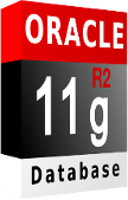
\includegraphics[scale=1]{oracle_11g}} &
            \multicolumn{1}{c}{
\includegraphics[scale=1]{ms_sql}} &
            \multicolumn{1}{c}{\textbf{Bedeutung}} \\
            \hline
          }
          \tabletail{
            \hline
          }
          \tablelasttail{
            \hline
          }
          \begin{supertabular}{|l|l|p{8cm}|}
            \identifier{NUMBER} & \identifier{NUMERIC} & Numerische Datentypen
            mit fester Genauigkeit und fester Anzahl von Dezimalstellen. \\
            \hline
            \identifier{DATE} & \identifier{DATETIME2} & Datums- und
            Zeitdatentypen zum Darstellen von Datum und Tageszeit. \\
            \hline
            \identifier{TIMESTAMP} & \identifier{DATETIME2} & Ein Datums- und
            Zeitdatentyp mit höherer Genauigkeit als \identifier{DATE}. \\
            \hline
            \identifier{VARCHAR2} & \identifier{VARCHAR} &
            Nicht-Unicode-Zeichendaten variabler Länge. \\
            \hline
            \identifier{CHAR} & \identifier{CHAR} & Nicht-Unicode-Zeichendaten
            fester Länge \\
          \end{supertabular}
        \end{small}
      \end{center}
      \subsection{Numerische Datentypen}
        \subsubsection{Aufbau}
          Die beiden Datentypen \identifier{NUMBER} (Oracle) und
          \identifier{NUMERIC} (SQL Server) sind dazu da, um positive oder
          negative numerische Werte, mit oder ohne Nachkommastellen,
          aufzunehmen. Die Wertebereiche, die beide Datentypen aufnehmen
          können, unterscheiden sich.
\clearpage
          \begin{center}
            \tablecaption{Datentypen}
            \label{numericranges}
            \begin{small}
              \tablefirsthead{
                \multicolumn{1}{c}{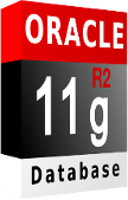
\includegraphics[scale=1]{oracle_11g}} &
                \multicolumn{1}{c}{
\includegraphics[scale=1]{ms_sql}} &
                \multicolumn{1}{c}{\textbf{Wertebereich}} \\
                \hline
              }
              \tabletail{
                \hline
              }
              \begin{supertabular}{|l|l|p{8cm}|}
                \identifier{NUMBER} & & $\pm1.0*10^{-130}$ bis $\pm1.0*10^{126}-1$ \\
                \hline
                & \identifier{NUMERIC} & $-1.0*10^{-38}$ bis $1.0*10^{38}-1$ \\
              \end{supertabular}
            \end{small}
          \end{center}
          \begin{merke}
            Zahlen die größer oder kleiner als die angegebenen
            Wertebereiche sind, können nicht aufgenommen werden.
          \end{merke}
        \subsubsection{Präzision und Skalarität}
          Unter der Präzision versteht man die Angabe, bei wie vielen Stellen
          insgesamt noch ein rundungsfehlerfreies Ergebnis angezeigt werden
          kann. Die maximale Präzision beider Typen beschränkt sich auf
          Zahlen, die kleiner oder gleich $10^{38}$ sind. Daraus folgt, dass
          solange sich eine Zahl in diesem Wertebereich befindet, sie frei von
          Rundungsfehlern ist. Ist sie größer, können Rundungsfehler
          auftreten. Beim Microsoft SQL Server stellt sich diese Problematik
          nicht, da bei \identifier{NUMERIC} der Wertebereich auf $10^{38}$
          beschränkt ist.

          Um die benötigte Präzision einstellen zu können, ist es auf beiden Systemen möglich, die maximale Anzahl Stellen, die eine Tabellenspalte aufnehmen können soll, auf einen Wert zwischen 1 und 38 einzuschränken. Ist eine Spalte, z. B. auf neun Stellen begrenzt, ist die größte Zahl, die in diese Spalte eingefügt werden kann, die 999.999.999.

          Mit Hilfe der Skalarität kann manuell festgelegt werden, wie viele der durch die Präzision angegebenen Stellen rechts vom Komma verwendet werden. Wird eine Spalte mit einer Präzision von neun und einer Skalarität von zwei definiert, kann sie maximal sieben Stellen links und zwei Stellen rechts vom Komma enthalten. Die größte Zahl, die in eine solche Spalte eingefügt werden kann, ist somit die 9.999.999,99.
      \subsection{Zeichendatentypen}
        \subsubsection{Typen fester Länge}
          Bei den Zeichendatentypen wird nach Typen fester Länge und Typen variabler Länge unterschieden. Der Datentyp zur Aufnahme von Zeichenketten fester Länge, heißt in beiden Systemen \identifier{CHAR}. Datentypen fester Länge haben ihren Namen daher, dass bei der Definition einer Tabellenspalte, mit einem solchen Typ, die Länge der Spalte fest angegeben werden muss.

          \begin{merke}
            Der Speicherplatzverbrauch einer solchen Spalte richtet sich nicht nach ihrem Inhalt (Anzahl der enthaltenen Zeichen), sondern nach der vorgegebenen Größe. Wird eine Spalte mit einer Größe von 20 definiert, beträgt ihr Speicherplatzverbrauch 20, 40 oder 80 Byte\footnote{Je nach dem, welcher Zeichensatz verwendet wird, werden pro Zeichen 1, 2 oder 4 Byte Speicherplatz benötigt.}. Dies trifft auch dann zu, wenn die Spalte nur ein einziges Zeichen enthält.
          \end{merke}
        \subsubsection{Typen variabler Länge}
          Die Zeichendatentypen variabler Länge unterscheiden sich in Oracle und SQL Server nur in ihrem Namen. SQL Server verwendet die SQL-92-Standard gemäße Bezeichnung \identifier{VARCHAR}, während Oracle die Bezeichnung \identifier{VARCHAR2}, als Synonym für VARCHAR verwendet. Die Nutzung von \identifier{VARCHAR} ist aber auch in Oracle zulässig.

          \begin{merke}
            Im Unterschied zu den Typen fester Länge, ergibt sich der Speicherplatzverbrauch bei Typen variabler Länge nicht durch eine fest definierte Größe, sondern anhand ihres Inhalts. Es kann eine maximale Größe angegeben werden. Die Spalte kann dann maximal so viele Zeichen aufnehmen, wie angegeben.
          \end{merke}
        \subsection{Datums- und Zeittypen}
          Zur Speicherung von Datums- und Zeitwerten kennt Oracle die beiden Datentypen \identifier{DATE} und \identifier{TIMESTAMP}. Microsoft SQL Server verwendet \identifier{DATETIME2}.

          \begin{merke}
            In MS SQL Server gibt es auch einen Datentyp \identifier{TIMESTAMP}. Dieser ist jedoch, abweichend vom SQL-2003-Standard, nicht zur Speicherung von Datums- und Zeitwerten vorgesehen und seit SQL Server 2008 als veraltet eingestuft.
          \end{merke}
          \subsubsection{Oracle - DATE und TIMESTAMP}
            Der Datentyp \identifier{DATE} speichert seine Datumswerte in einem internen, numerischen Format. Er berücksichtigt dabei: Jahrzehnt, Jahr, Monat, Tag, Stunde, Minute, Sekunde. Der Typ \identifier{TIMESTAMP} ist eine Erweiterung. Er kann Datums- und Zeitangaben auf bis zu 9 Stellen (Nanosekunde) genau, im Sekundenbereich speichern.
          \subsubsection{SQL Server - DATETIME2}
            Werte des \identifier{DATETIME2}-Datentyps werden von der Microsoft SQL Server 2008 R2 Database Engine (Datenbankmodul) intern, als zwei 4 Byte lange, ganze Zahlen, gespeichert. Die ersten 4 Byte enthalten die Anzahl von Tagen, vor oder nach dem Referenzdatum, dem 1. Januar 1900. Die anderen 4 Byte speichern die Tageszeit, die als Anzahl von Millisekunden seit Mitternacht dargestellt wird.
    \section{Konvertierung von Datentypen}
      Unter der Konvertierung von Datentypen versteht man das Umwandeln eines Wertes, eines bestimmten Typs, in einen anderen Typ. Beispielsweise kann eine Zeichenkette \enquote{1234} in die gleichlautende Zahl \enquote{1234} umgewandelt werden. Intern wird nur der Datentyp von VARCHAR/VARCHAR2 auf NUMERIC/NUMBER geändert. Dies ist z. B. notwendig, um arithmetische Operationen durchzuführen.
      \subsection{Implizite Datentypkonvertierung}
        \begin{merke}
				Unter der impliziten Konvertierung versteht man, dass automatische Umwandeln eines Datentyp durch das DBMS in einen Anderen.
        \end{merke}
        In \beispiel{sql03_27} wird die implizite Konvertierung der Gehälter in Zeichenketten gezeigt.
        \begin{lstlisting}[language=oracle_sql,caption={Implizite Konvertierung von \identifier{NUMBER} zu \identifier{VARCHAR2}},label=sql03_27]
SELECT 'Das Gehalt von ' || Nachname || ' betraegt: ' || gehalt
       AS "Implizite Konvertierung"
FROM   Mitarbeiter;
        \end{lstlisting}
        \begin{center}
          \begin{small}
            \changefont{pcr}{m}{n}
            \tablefirsthead {
              \multicolumn{1}{l}{\textbf{Implizite Konvertierung}} \\
              \cmidrule(l){1-1}
            }
            \tablehead{}
            \tabletail {
              \multicolumn{1}{l}{\textbf{101 Zeilen ausgewählt}} \\
            }
            \tablelasttail {
              \multicolumn{1}{l}{\textbf{101 Zeilen ausgewählt}} \\
            }
            \begin{oraclesql}
              \begin{supertabular}{l}
                Das Gehalt von Winter betraegt: 88000 \\
                Das Gehalt von Werner betraegt: 50000 \\
                Das Gehalt von Seifert betraegt: 50000 \\
                Das Gehalt von Schwarz betraegt: 30000 \\
              \end{supertabular}
            \end{oraclesql}
          \end{small}
        \end{center}
\clearpage
        Damit Oracle eine Ausgabe wie \enquote{Das Gehalt von Winter betraegt:
        88000} darstellen kann, muss ein einheitlicher Datentyp geschaffen
        werden. Hierzu wird ein Ausdruck in zwei Teile zerlegt, einen linken und
        einen rechten. Der rechte Teil wird dann, sofern möglich, in den
        Datentyp des Linken konvertiert. Für \beispiel{sql03_27} bedeutet dies
        konkret:
        \begin{itemize}
          \item Linke Seite: \languageorasql{'Das Gehalt von ' || Nachname || ' betraegt: '}
          \item Rechte Seite: \languageorasql{Gehalt}
          \item Datentyp der linken Seite: \identifier{VARCHAR2}
          \item Datentyp der rechten Seite: \identifier{NUMBER}
          \item Daraus folgt: Konvertiere \identifier{NUMBER} nach \identifier{VARCHAR2}
        \end{itemize}
        Nicht immer ist das Konvertieren eines Datentyps in einen anderen möglich. Für die implizite Konvertierung gibt es einige Einschränkungen.
        \begin{itemize}
          \item Der Wert selbst muss in den neuen Typ konvertierbar sein. Beispielsweise kann die Zeichenkette ABCDE nicht in eine Zahl oder ein Datum umgewandelt werden, da sie kein sinnvolles Datum darstellt.
          \item Der Datentyp selbst muss in den neuen Datentyp konvertierbar sein. Zum Beispiel kann Oracle einen Wert des Datentyps NUMBER nicht direkt in einen Wert des Typs DATE konvertieren, da hierzu ein Referenzdatum benötigt wird.
        \end{itemize}
        Die beiden folgenden Tabellen zeigen, welche impliziten Typkonvertierung in Oracle und SQL Server möglich sind. Dabei wird immer zugrunde gelegt, dass der betreffende Wert auch konvertierbar ist.
        \begin{center}
          \tablecaption{Implizite Datentypkonvertierung in Oracle}
          \label{oracleimplicit}
          \begin{small}
            \tablefirsthead{
              \multicolumn{6}{c}{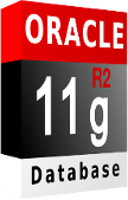
\includegraphics[scale=1]{oracle_11g}} \\
              \multicolumn{1}{c}{} &
              \multicolumn{1}{c}{\textbf{NUMBER}} &
              \multicolumn{1}{c}{\textbf{VARCHAR2}} &
              \multicolumn{1}{c}{\textbf{CHAR}} &
              \multicolumn{1}{c}{\textbf{DATE}} &
              \multicolumn{1}{c}{\textbf{TIMESTAMP}} \\
              \hline
            }
            \tabletail{
              \hline
            }
            \tablelasttail{
              \hline
            }
            \begin{supertabular}{|l|c|c|c|c|c|}
              NUMBER    & -- & X  & X  & -- & -- \\
              \hline
              VARCHAR2  & X  & -- & X  & X  & X \\
              \hline
              CHAR      & X  & X  & -- & X  & X \\
              \hline
              DATE      & -- & X  & X  & -- & -- \\
              \hline
              TIMESTAMP & X  & X  & X  & -- & -- \\
            \end{supertabular}
          \end{small}
        \end{center}
\clearpage
        \begin{center}
          \tablecaption{Implizite Datentypkonvertierung in Microsoft SQL Server}
          \label{mssqlimplicit}
          \begin{small}
            \tablefirsthead{
              \multicolumn{5}{c}{
\includegraphics[scale=1]{ms_sql}} \\
              \multicolumn{1}{c}{} &
              \multicolumn{1}{c}{\textbf{NUMERIC}} &
              \multicolumn{1}{c}{\textbf{VARCHAR}} &
              \multicolumn{1}{c}{\textbf{CHAR}} &
              \multicolumn{1}{c}{\textbf{DATETIME2}} \\
              \hline
            }
            \tabletail{
              \hline
            }
            \tablelasttail{
              \hline
            }
            \begin{supertabular}{|l|c|c|c|c|}
              NUMERIC   & -- & X  & X  & X \\
              \hline
              VARCHAR   & X  & -- & X  & X \\
              \hline
              CHAR      & X  & X  & -- & X \\
              \hline
              DATETIME  & -- & X  & X  & -- \\
            \end{supertabular}
          \end{small}
        \end{center}
        \begin{merke}
            Der SQL Server besitzt intern eine Rangfolge seiner Datentypen. Dadurch wird bei der impliziten Konvertierung der Datentyp mit der niedrigeren Rangfolge in den Datentyp mit der höheren Rangfolge umgewandelt.
        \end{merke}
        \begin{literaturinternet}
          \item \cite{autoId8}
          \item \cite{ms191530}
          \item \cite{ms190309}
        \end{literaturinternet}
      \subsection{Explizite Datentypkonvertierung}
        \subsubsection{Explizite Datentypkonvertierung in Oracle}
          \begin{merke}
            Bei der expliziten Datentypkonvertierung werden Werte, mit Hilfe von
            Funktionen, von einem Datentyp in einen anderen konvertiert.
          \end{merke}
          Oracle kennt für das explizite Konvertieren von Daten verschiedene
          Funktionen. Diese sind:
          \begin{itemize}
            \item \languageorasql{TO\_CHAR}
            \item \languageorasql{TO\_DATE}
            \item \languageorasql{TO\_TIMESTAMP}
            \item \languageorasql{TO\_NUMBER}
          \end{itemize}
          Es existieren noch weitere Funktionen, die an dieser Stelle jedoch
          ungenannt bleiben. Die folgende Tabelle zeigt eine Übersicht, welche
          Datentypen, mit Hilfe der expliziten Datentypkonvertierung umgewandelt
          werden können.
          \begin{center}
            \tablecaption{Explizite Datentypkonvertierung in Oracle}
            \label{oracleexplicit}
            \begin{small}
              \tablefirsthead{
                \multicolumn{6}{c}{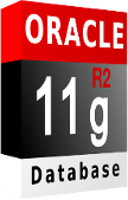
\includegraphics[scale=1]{oracle_11g}} \\
                \multicolumn{1}{c}{} &
                \multicolumn{1}{c}{\textbf{NUMBER}} &
                \multicolumn{1}{c}{\textbf{VARCHAR2}} &
                \multicolumn{1}{c}{\textbf{CHAR}} &
                \multicolumn{1}{c}{\textbf{DATE}} &
                \multicolumn{1}{c}{\textbf{TIMESTAMP}} \\
                \hline
              }
              \tabletail{
                \hline
              }
              \begin{supertabular}{|l|c|c|c|c|c|}
                NUMBER    & -- & TO\_CHAR & TO\_CHAR            &          & -- \\
                \hline
                VARCHAR2  & TO\_NUMBER    & --       & --       & TO\_DATE & TO\_TIMESTAMP \\
                \hline
                CHAR      & TO\_NUMBER    & --       & --       & TO\_DATE & TO\_TIMESTAMP \\
                \hline
                DATE      & --            & TO\_CHAR & TO\_CHAR & --       & TO\_TIMESTAMP \\
                \hline
                TIMESTAMP & --            & TO\_CHAR & TO\_CHAR & --       & -- \\
              \end{supertabular}
            \end{small}
          \end{center}
          \beispiel{sql03_28} zeigt die Umwandlung des Systemdatums in eine
          Zeichenkette.
          \begin{lstlisting}[language=oracle_sql,caption={Explizite Datentypkonvertierung in Oracle},label=sql03_28]
SELECT TO_CHAR(SYSDATE)
FROM   dual;
          \end{lstlisting}
          \begin{center}
            \begin{small}
              \changefont{pcr}{m}{n}
              \tablefirsthead {
                \multicolumn{1}{l}{\textbf{TO\_CHAR(SYSDATE)}} \\
                \cmidrule(l){1-1}
              }
              \tablehead{}
              \tabletail {
%                 \multicolumn{1}{l}{\textbf{1 Zeile ausgewählt}} \\
              }
              \tablelasttail {
                \multicolumn{1}{l}{\textbf{1 Zeile ausgewählt}} \\
              }
              \begin{oraclesql}
                \begin{supertabular}{l}
                  02.05.13 \\
                \end{supertabular}
              \end{oraclesql}
            \end{small}
          \end{center}
          Tatsächlich geschieht in \beispiel{sql03_28} nichts sichtbares,
          dennoch hat eine Umwandlung stattgefunden. Um diese sichtbar zu
          machen, kann während der Konvertierung eine Formatierung des
          Ergebniswertes durchgeführt werden.
          \begin{lstlisting}[language=oracle_sql,caption={Konvertierung und Formatierung},label=sql03_29]
SELECT TO_CHAR(SYSDATE, 'DD.MM.YYYY')
FROM   dual;
          \end{lstlisting}
          \begin{center}
            \begin{small}
              \changefont{pcr}{m}{n}
              \tablefirsthead {
                \multicolumn{1}{l}{\textbf{TO\_CHAR(SYSDATE,'DD.MM.YYYY')}} \\
                \cmidrule(l){1-1}
              }
              \tablehead{}
              \tabletail {
                \multicolumn{1}{l}{\textbf{1 Zeile ausgewählt}} \\
              }
              \tablelasttail {
                \multicolumn{1}{l}{\textbf{1 Zeile ausgewählt}} \\
              }
              \begin{oraclesql}
                \begin{supertabular}{l}
                  02.05.2013 \\
                \end{supertabular}
              \end{oraclesql}
            \end{small}
          \end{center}
          Das zweite Argument der \languageorasql{TO\_CHAR}-Funktion, \languageorasql{'DD.MM.YYYY'}, wird als \enquote{Formatmodell} bezeichnet. Mit Hilfe dieser Buchstabenkombination wird das Ausgabeformat für die Zeichenfolge festgelegt. Die Bedeutung der Buchstaben ist:
          \begin{itemize}
            \item \languageorasql{DD}: Tag 2-stellig
            \item \languageorasql{MM}: Monat 2-stellig
            \item \languageorasql{YYYY}: Jahr 4-stellig
          \end{itemize}
          \beispiel{sql03_30} zeigt ein weiteres, individuelles Formatmodell für einen Datumswert.
          \begin{lstlisting}[language=oracle_sql,caption={Ein anderes Formatmodell},label=sql03_30]
SELECT TO_CHAR(SYSDATE, 'DD. MON YYYY')
FROM   dual;
          \end{lstlisting}
          \begin{center}
            \begin{small}
              \changefont{pcr}{m}{n}
              \tablefirsthead {
                \multicolumn{1}{l}{\textbf{TO\_CHAR(SYSDATE,'DD.MONYYYY')}} \\
                \cmidrule(l){1-1}
              }
              \tablehead{}
              \tabletail {
                \multicolumn{1}{l}{\textbf{1 Zeile ausgewählt}} \\
              }
              \tablelasttail {
                \multicolumn{1}{l}{\textbf{1 Zeile ausgewählt}} \\
              }

              \begin{oraclesql}
                \begin{supertabular}{l}
                  02. MAI 2013 \\
                \end{supertabular}
              \end{oraclesql}
            \end{small}
          \end{center}
          Die Buchstabenkombination \languageorasql{MON} sorgt dafür, dass der Monat als Wort angezeigt wird. Ob \enquote{Mai} oder \enquote{May} angezeigt wird, ist abhängig von den Ländereinstellungen der Datenbank.

          \begin{merke}
            Ein Formatmodell ist eine Zeichenfolge, die das Format eines Datums oder eines numerischen Wertes beschreibt. Ein Formatmodell ändert nicht die interne Darstellung eines Wertes in der Datenbank, sondern formatiert lediglich die Ausgabe. Es setzt sich aus mehreren Formatelemten zusammen, z. B. DD oder MM oder YYYY.
          \end{merke}
          Welche Formatmodelle erstellt werden können, hängt davon ab, welche Formatelemte die einzelnen Funktionen kennen. Die folgenden Literaturhinweise führen zu den Tabellen in der Oracle Online-Dokumentation, die alle existierenden Formatelemente enthält.
          \begin{literaturinternet}
            \item \cite{i34570}
            \item \cite{i34924}
          \end{literaturinternet}

          \begin{merke}
            Für die Funktion \languageorasql{TO\_CHAR} existiert keine eigenständige Zusammenstellung von Formatelementen, da sie sowohl Datumswerte in Text, als auch Zahlen in Text konvertiert und dafür die Formatelemente von \languageorasql{TO\_NUMBER} und \languageorasql{TO\_DATE} nutzt.
          \end{merke}
        \subsubsection{Explizite Datentypkonvertierung in Microsoft SQL Server}
          \begin{merke}
            Bei der expliziten Datentypkonvertierung werden Werte, mit Hilfe von Funktionen, von einem Datentyp in einen anderen konvertiert.
          \end{merke}
          MS SQL Server kennt die Funktion \languagemssql{CONVERT} zur Konvertierung von Datentypen \footnote{Es gibt zusätzlich die Funktion CAST. Jedoch wird seitens Microsoft empfohlen, \languagemssql{CONVERT} zu nutzen, obgleich die Verwendung von CAST dem ISO-Standard entsprechen würde.}. Die Syntax dieser Funktion lautet:
          \begin{lstlisting}[language=ms_sql,caption={Die Syntax der CONVERT-Funktion in MS SQL Server},label=sql03_31]
CONVERT( <Datentyp>[(Laenge)], <Ausdruck>[, Style])
          \end{lstlisting}
          \begin{center}
            \tablecaption{Funktionsargumente von CONVERT}
            \label{argconvert}
            \begin{small}
              \tablefirsthead{
                \multicolumn{1}{c}{\textbf{Argument}} &
                \multicolumn{1}{c}{\textbf{Beispiel}} &
                \multicolumn{1}{c}{\textbf{Erläuterung}} \\
                \hline
              }
              \tabletail{
                \hline
              }
              \tablelasttail{
                \hline
              }
              \begin{supertabular}{|l|c|p{8.5cm}|}
                \textless Datentyp\textgreater & DATETIME & Dies ist die Angabe des Datentyps, in den \textless Ausdruck\textgreater\ konvertiert werden soll.  Für jeden Datentyp kann optional eine Länge mit angegeben werden.\\
                \hline
                \textless Ausdruck\textgreater & '16.01.2009'& <Ausdruck> ist eine Zeichenkette, Zahl, ein Datums- Zeitwert oder eine Funktion. \\
                \hline
                [Style] & 104 & Optional kann bei der CONVERT-Funktion ein Formatmodell angegeben werden. \\
              \end{supertabular}
            \end{small}
          \end{center}
          Ein Formatmodell legt fest, wie ein Eingabewert interpretiert oder ein Ausgabewert formatiert werden soll. Alle Formatmodelle sind durch Zahlen kodiert.

          Die Bedeutung der Formatmodelle soll konkret anhand von \beispiel{sql03_32} erläutert werden.
          \begin{lstlisting}[language=ms_sql,caption={CONVERT mit Formatmodell},label=sql03_32]
SELECT CONVERT(DATETIME2, '02.05.2013', 104)
          \end{lstlisting}
          \begin{center}
            \begin{small}
              \changefont{pcr}{m}{n}
              \tablefirsthead{
                \multicolumn{1}{l}{\textbf{(Kein Spaltenname)}} \\
                \cmidrule(l){1-1}
              }
              \tabletail{}
              \tablelasttail{}
              \begin{mssql}
                \begin{supertabular}{l}
                  2013-05-02 00:00:00.0000000 \\
                \end{supertabular}
              \end{mssql}
            \end{small}
          \end{center}
          \beispiel{sql03_32} zeigt die Konvertierung der Zeichenkette \enquote{02.05.2013} in ein Datum. Damit dies korrekt ablaufen kann, muss die Datenbank wissen, wie die einzelnen Teile der Zeichenkette zu verstehen sind. Die Formatmodellnummer 104 besagt, dass der angegebene Ausdruck im Format \enquote{DD.MM.YYYY} zu interpretieren ist.

          Was passiert, wenn ein zum Ausdruck inkompatibles Formatmodell angegeben wird, zeigt \beispiel{sql03_32}. Das Formatmodell \enquote{4} liest den Ausdruck \enquote{02.05.2013} als \enquote{DD.MM.YY} (2-stellige Jahreszahl). Da der Ausdruck aber mit 4-stelliger Jahreszahl angegeben ist, führt dieses Beispiel zu einer Fehlermeldung.
          \begin{lstlisting}[language=ms_sql,caption={CONVERT mit falschem Formatmodell},label=sql03_33]
SELECT CONVERT(DATETIME2, '02.05.2013', 4)

Meldung 241, Ebene 16, Status 1, Zeile 1
Fehler beim Konvertieren einer Zeichenfolge in einen datetime-Wert.
          \end{lstlisting}
          In \beispiel{sql03_32} diente \languagemssql{CONVERT} dazu, um die Zeichenfolge \enquote{02.05.2013} korrekt zu interpretieren (Eingabeformat). Die gleiche Funktion kann aber auch das Ausgabeformat eines Ausdrucks bestimmen. \beispiel{sql03_34} zeigt, wie das aktuelle Systemdatum in eine Zeichenkette konvertiert wird. Dabei wird die 2-stellige Jahresangabe in eine 4-stellige umformatiert.
%\clearpage
          \begin{lstlisting}[language=ms_sql,caption={Formatieren den Ausgabe mit \languagemssql{CONVERT}},label=sql03_34]
SELECT GETDATE(), CONVERT(VARCHAR, GETDATE(), 104)
          \end{lstlisting}
          \begin{center}
            \begin{small}
              \changefont{pcr}{m}{n}
              \tablefirsthead{
                \multicolumn{1}{l}{\textbf{(Kein Spaltenname)}} &
                \multicolumn{1}{l}{\textbf{(Kein Spaltenname)}} \\
                \cmidrule(l){1-1}\cmidrule(l){2-2}
              }
              \tabletail{}
              \tablelasttail{}
              \begin{mssql}
                \begin{supertabular}{ll}
                  2013-05-02 17:18:24.763 & 02.05.2013 \\
                \end{supertabular}
              \end{mssql}
            \end{small}
          \end{center}
          Welche Formatmodelle SQL Server kennt ist unter dem folgenden Literaturhinweis nachlesbar.
        \begin{literaturinternet}
          \item \cite{ms191530}
        \end{literaturinternet}

    \clearpage
    \section{Übungen - Funktionen}
      \begin{enumerate}
        \item Lassen Sie das aktuelle Datum auf dem Bildschirm ausgeben und
        benennen Sie die Spalte mit \enquote{Datum}.
        \begin{center}
          \begin{small}
            \changefont{pcr}{m}{n}
            \tablefirsthead {
              \multicolumn{1}{l}{\textbf{Datum}} \\
              \cmidrule(l){1-1}
            }
            \tablehead{}
            \tabletail {
              \multicolumn{1}{l}{\textbf{1 Zeile ausgewählt}} \\
            }
            \tablelasttail {
              \multicolumn{1}{l}{\textbf{1 Zeile ausgewählt}} \\
            }
            \begin{msoraclesql}
              \begin{supertabular}{l}
                12.05.13 \\
              \end{supertabular}
            \end{msoraclesql}
          \end{small}
        \end{center}
        \item Lassen Sie das aktuelle Datum mit Uhrzeit auf dem Bildschirm
        ausgeben und benennen Sie die Spalte mit \enquote{Datum/Uhrzeit}.
        \begin{center}
          \begin{small}
            \changefont{pcr}{m}{n}
            \tablefirsthead {
              \multicolumn{1}{l}{\textbf{Datum/Uhrzeit}} \\
              \cmidrule(l){1-1}
            }
            \tablehead{}
            \tabletail {
              \multicolumn{1}{l}{\textbf{1 Zeile ausgewählt}} \\
            }
            \tablelasttail {
              \multicolumn{1}{l}{\textbf{1 Zeile ausgewählt}} \\
            }
            \begin{msoraclesql}
              \begin{supertabular}{l}
                12.05.13 10:58:45,439419 +02:00 \\
              \end{supertabular}
            \end{msoraclesql}
          \end{small}
        \end{center}
        \item Schreiben Sie eine Abfrage, welche die Mitarbeiternummer, den
        Nachnamen, das Gehalt und ein um 3,5 \% erhöhtes Gehalt für jeden
        Mitarbeiter anzeigt. Das erhöhte Gehalt soll als ganze Zahl und mit
        dem Spaltenalias \enquote{Neues Gehalt} ausgegeben werden!
        \begin{center}
          \begin{small}
            \changefont{pcr}{m}{n}
            \tablefirsthead {
              \multicolumn{1}{r}{\textbf{MITARBEITER\_ID}} &
              \multicolumn{1}{l}{\textbf{NACHNAME}} &
              \multicolumn{1}{r}{\textbf{GEHALT}} &
              \multicolumn{1}{r}{\textbf{Neues Gehalt}} \\
              \cmidrule(r){1-1}\cmidrule(l){2-2}\cmidrule(r){3-3}\cmidrule(r){4-4}
            }
            \tablehead{}
            \tabletail {
              \multicolumn{4}{l}{\textbf{100 Zeilen ausgewählt}} \\
            }
            \tablelasttail {
              \multicolumn{4}{l}{\textbf{100 Zeilen ausgewählt}} \\
            }
            \begin{msoraclesql}
              \begin{supertabular}{rlrr}
                1 & Winter & 88000 & 91080 \\
                2 & Werner & 50000 & 51750 \\
                3 & Seifert & 50000 & 51750 \\
                4 & Schwarz & 30000 & 31050 \\
              \end{supertabular}
            \end{msoraclesql}
          \end{small}
        \end{center}
        \item Verändern Sie die Abfrage, aus der vorangegangenen Aufgabe so,
        dass eine zusätzliche Spalte hinzugefügt wird, die die Differenz
        zwischen dem alten und dem erhöhten Gehalt anzeigt. Benennen Sie die
        Spalte mit \enquote{Gehaltserhoehung}.
        \begin{center}
          \begin{small}
            \changefont{pcr}{m}{n}
            \tablefirsthead {
              \multicolumn{1}{r}{\textbf{MITARBEITER\_ID}} &
              \multicolumn{1}{l}{\textbf{NACHNAME}} &
              \multicolumn{1}{r}{\textbf{GEHALT}} &
              \multicolumn{1}{r}{\textbf{Neues Gehalt}} &
              \multicolumn{1}{r}{\textbf{Gehaltserhöhung}} \\
              \cmidrule(r){1-1}\cmidrule(l){2-2}\cmidrule(r){3-3}\cmidrule(r){4-4}\cmidrule(r){5-5}
            }
            \tablehead{}
            \tabletail {
%               \multicolumn{5}{l}{\textbf{100 Zeilen ausgewählt}} \\
            }
            \tablelasttail {
              \multicolumn{5}{l}{\textbf{100 Zeilen ausgewählt}} \\
            }
            \begin{msoraclesql}
              \begin{supertabular}{rlrrr}
                1 & Winter & 88000 & 91080 & 3080 \\
                2 & Werner & 50000 & 51750 & 1750 \\
                3 & Seifert & 50000 & 51750 & 1750 \\
                4 & Schwarz & 30000 & 31050 & 1050 \\
              \end{supertabular}
            \end{msoraclesql}
          \end{small}
        \end{center}
\clearpage
        \item Zeigen Sie die Nachnamen und die Länge der Nachnamen aller
        Mitarbeiter an, deren Nachname mit einem der Buchstaben \enquote{J},
        \enquote{M} oder \enquote{S} beginnt. Die Spalten sollen, wie in der
        Lösung zu sehen ist, beschriftet sein. Die Nachnamen müssen in
        Großbuchstaben ausgegeben werden. Sortieren Sie die Abfrage in
        absteigender Reihenfolge nach den Nachnamen! 
        \begin{center}
          \begin{small}
            \changefont{pcr}{m}{n}
            \tablefirsthead {
              \multicolumn{1}{l}{\textbf{Nachname}} &
              \multicolumn{1}{r}{\textbf{Laenge}} \\
              \cmidrule(l){1-1}\cmidrule(r){2-2}
            }
            \tablehead{}
            \tabletail {
              \multicolumn{2}{l}{\textbf{23 Zeilen ausgewählt}} \\
            }
            \tablelasttail {
              \multicolumn{2}{l}{\textbf{23 Zeilen ausgewählt}} \\
            }
            \begin{msoraclesql}
              \begin{supertabular}{lr}
                SINDERMANN & 10 \\
                SINDERMANN & 10 \\
                SIMON & 5 \\
                SIMON & 5 \\
                SIMON & 5 \\
                SEIFERT & 7 \\
                SEIFERT & 7 \\
                SCHWARZ & 7 \\
                SCHWARZ & 7 \\
              \end{supertabular}
            \end{msoraclesql}
          \end{small}
        \end{center}
        \item Zeigen Sie für jeden Mitarbeiter den Nachnamen an, sein Geburtsdatum und seit wie vielen Monaten dieser bereits 18 Jahre alt ist        (gerundet auf zwei Stellen, nach dem Komma). Benennen Sie die Spalte mit den Monaten: \enquote{Alter in Monaten}. Sortieren Sie die Abfrage in
        aufsteigender Reihenfolge nach der Spalte \enquote{Alter in Monaten}.

        \begin{merke}
          Zur Lösung dieser Aufgabe mit Oracle soll die Funktion \languageorasql{MONTHS_BETWEEN} herangezogen werden, deren Syntax der Oracle Onlinedokumentation entnommen werden kann.
        \end{merke}
        \begin{center}
          \begin{small}
            \changefont{pcr}{m}{n}
            \tablefirsthead {
              \multicolumn{1}{l}{\textbf{NACHNAME}} &
              \multicolumn{1}{l}{\textbf{GEBURTSDATUM}} &
              \multicolumn{1}{r}{\textbf{Alter in Monaten}} \\
              \cmidrule(l){1-1}\cmidrule(l){2-2}\cmidrule(r){3-3}
            }
            \tablehead{}
            \tabletail {
%               \multicolumn{3}{l}{\textbf{100 Zeilen ausgewählt}} \\
            }
            \tablelasttail {
              \multicolumn{3}{l}{\textbf{100 Zeilen ausgewählt}} \\
            }
            \begin{msoraclesql}
              \begin{supertabular}{llr}
                Krüger & 31.05.93 & 23,4 \\
                Walther & 07.01.93 & 28,18 \\
                Lehmann & 07.11.92 & 30,18 \\
                Keller & 04.11.92 & 30,27 \\
                Schwarz & 27.06.92 & 34,53 \\
                Weber & 10.06.92 & 35,08 \\
                Peters & 13.05.92 & 35,98 \\
                Köhler & 05.05.92 & 36,24 \\
                Lorenz & 13.12.91 & 40,98 \\
              \end{supertabular}
            \end{msoraclesql}
          \end{small}
        \end{center}
\clearpage
        \item Ermitteln Sie Vorname, Nachname und Geburtsdatum der Mitarbeiter,
        die mindestens 1 Jahr und 4 Monate nach dem \enquote{07.05.1978} geboren
        sind. Sortieren Sie die Abfrage in absteigender Reihenfolge nach dem
        Geburtsdatum.
        \begin{center}
          \begin{small}
            \changefont{pcr}{m}{n}
            \tablefirsthead {
              \multicolumn{1}{l}{\textbf{VORNAME}} &
              \multicolumn{1}{l}{\textbf{NACHNAME}} &
              \multicolumn{1}{l}{\textbf{GEBURTSDATUM}} \\
              \cmidrule(l){1-1}\cmidrule(l){2-2}\cmidrule(l){3-3}
            }
            \tablehead{}
            \tabletail {
              \multicolumn{3}{l}{\textbf{81 Zeilen ausgewählt}} \\
            }
            \tablelasttail {
              \multicolumn{3}{l}{\textbf{81 Zeilen ausgewählt}} \\
            }
            \begin{msoraclesql}
              \begin{supertabular}{lll}
                Emma & Krüger & 31.05.93 \\
                Lina & Walther & 07.01.93 \\
                Johannes & Lehmann & 07.11.92 \\
%                 Anna & Keller & 04.11.92 \\
              \end{supertabular}
            \end{msoraclesql}
          \end{small}
        \end{center}
        \item Zeigen Sie für jeden Mitarbeiter, der zum Zeitpunkt der Ausführung dieser Abfrage mindestens 35 Jahre alt ist, dessen Mitarbeiter\_ID, das Geburtsdatum und den Wochentag seiner Geburt an. Beschriften Sie die Spalten, wie in der Lösung vorgegeben. Ordnen Sie die Abfrage in aufsteigender Reihenfolge nach dem Wochentag, beginnend beim ersten Tag der Woche!
        \begin{center}
          \begin{small}
            \changefont{pcr}{m}{n}
            \tablefirsthead {
              \multicolumn{1}{r}{\textbf{MITARBEITER\_ID}} &
              \multicolumn{1}{l}{\textbf{GEBURTSDATUM}} &
              \multicolumn{1}{l}{\textbf{Wochentag}} \\
              \cmidrule(r){1-1}\cmidrule(l){2-2}\cmidrule(l){3-3}
            }
            \tablehead{}
            \tabletail {
              \multicolumn{3}{l}{\textbf{11 Zeilen ausgewählt}} \\
            }
            \tablelasttail {
              \multicolumn{3}{l}{\textbf{11 Zeilen ausgewählt}} \\
            }
            \begin{msoraclesql}
              \begin{supertabular}{rll}
                42 & 31.01.77 & MONTAG     \\
                90 & 14.12.76 & DIENSTAG   \\
                36 & 14.02.78 & DIENSTAG   \\
                2 & 03.11.77 & DONNERSTAG \\
                51 & 19.02.76 & DONNERSTAG \\
%                 67 & 08.10.76 & FREITAG    \\
              \end{supertabular}
            \end{msoraclesql}
          \end{small}
        \end{center}
        \item Schreiben Sie eine Abfrage, die für alle Mitarbeiter deren
        Nachnamen und die Bankfiliale\_ID anzeigt. Wenn ein Mitarbeiter in
        keiner Bankfiliale tätig ist, soll \enquote{Keine Bankfiliale}
        angezeigt werden.
        \begin{center}
          \begin{small}
            \changefont{pcr}{m}{n}
            \tablefirsthead {
              \multicolumn{1}{l}{\textbf{NACHNAME}} &
              \multicolumn{1}{l}{\textbf{BANKFILIALE}} \\
              \cmidrule(l){1-1}\cmidrule(l){2-2}
            }
            \tablehead{}
            \tabletail {
            }
            \tablelasttail {
              \multicolumn{2}{l}{\textbf{100 Zeilen ausgewählt}} \\
            }
            \begin{msoraclesql}
              \begin{supertabular}{ll}
                Möller & Keine Bankfiliale \\
                Winter & Keine Bankfiliale \\
                Meier & Keine Bankfiliale \\
                Sindermann & Keine Bankfiliale \\
                Schwarz & Keine Bankfiliale \\
                Werner & Keine Bankfiliale \\
                Krüger & 1 \\
                Peters & 1 \\
                Kipp & 1 \\
              \end{supertabular}
            \end{msoraclesql}
          \end{small}
        \end{center}
      \end{enumerate}

    \clearpage
\section{Lösungen - Funktionen}
\begin{enumerate}
    \item Lassen Sie das aktuelle Datum auf dem Bildschirm ausgeben und
          benennen Sie die Spalte mit \enquote{Datum}.
          \begin{oraclesql}[\FALSE]
          \end{oraclesql}
          \begin{lstlisting}[language=oracle_sql]
SELECT SYSDATE AS "Datum"
FROM   dual;
        \end{lstlisting}
          \begin{mssql}[\FALSE]
          \end{mssql}
          \begin{lstlisting}[language=ms_sql]
SELECT GETDATE() AS "Datum";
        \end{lstlisting}
    \item Lassen Sie das aktuelle Datum mit Uhrzeit auf dem Bildschirm
          ausgeben und benennen Sie die Spalte mit \enquote{Datum/Uhrzeit}.
          \begin{oraclesql}[\FALSE]
          \end{oraclesql}
          \begin{lstlisting}[language=oracle_sql]
SELECT SYSTIMESTAMP AS "Datum/Uhrzeit"
FROM   dual;
        \end{lstlisting}
          \begin{mssql}[\FALSE]
          \end{mssql}
          \begin{lstlisting}[language=ms_sql]
SELECT GETDATE() AS "Datum/Uhrzeit";
        \end{lstlisting}
    \item Schreiben Sie eine Abfrage, welche die Mitarbeiternummer, den
          Nachnamen, das Gehalt und ein um 3,5 \% erhöhtes Gehalt für jeden
          Mitarbeiter anzeigt. Das erhöhte Gehalt soll als ganze Zahl und mit
          dem Spaltenalias \enquote{Neues Gehalt} ausgegeben werden!
          \begin{oraclesql}[\FALSE]
          \end{oraclesql}
          \begin{lstlisting}[language=oracle_sql]
SELECT Mitarbeiter_ID, Nachname, Gehalt,
       ROUND(Gehalt * 1.035, 0) AS "Neues Gehalt"
FROM   Mitarbeiter;
        \end{lstlisting}
          \begin{mssql}[\FALSE]
          \end{mssql}
          \begin{lstlisting}[language=ms_sql]
SELECT Mitarbeiter_ID, Nachname, Gehalt,
       CEILING(ROUND(Gehalt * 1.035, 0)) AS "Neues Gehalt"
FROM   Mitarbeiter;
        \end{lstlisting}
    \item Verändern Sie die Abfrage, aus der vorangegangenen Aufgabe so,
          dass eine zusätzliche Spalte hinzugefügt wird, die die Differenz
          zwischen dem alten und dem erhöhten Gehalt anzeigt. Benennen Sie die
          Spalte mit \enquote{Gehaltserhoehung}.
          \begin{oraclesql}[\FALSE]
          \end{oraclesql}
          \begin{lstlisting}[language=oracle_sql]
SELECT Mitarbeiter_ID, Nachname, Gehalt,
       ROUND(Gehalt * 1.035, 0) AS "Neues Gehalt",
       ROUND(Gehalt * 1.035, 0) - Gehalt AS "Gehaltserhoehung"
FROM   Mitarbeiter;
        \end{lstlisting}
          \begin{mssql}[\FALSE]
          \end{mssql}
          \begin{lstlisting}[language=ms_sql]
SELECT Mitarbeiter_ID, Nachname, Gehalt,
       CEILING(ROUND(Gehalt * 1.035, 0)) AS "Neues Gehalt",
       CEILING(ROUND(Gehalt * 1.035, 0)) - Gehalt AS "Gehaltserhoehung"
FROM   Mitarbeiter;
        \end{lstlisting}
    \item Zeigen Sie die Nachnamen und die Länge der Nachnamen aller
          Mitarbeiter an, deren Nachname mit einem der Buchstaben \enquote{J},
          \enquote{M} oder \enquote{S} beginnt. Die Spalten sollen, wie in der
          Lösung zu sehen ist, beschriftet sein. Die Nachnamen müssen in
          Großbuchstaben ausgegeben werden. Sortieren Sie die Abfrage in
          absteigender Reihenfolge nach den Nachnamen!
          \begin{oraclesql}[\FALSE]
          \end{oraclesql}
          \begin{lstlisting}[language=oracle_sql]
SELECT  UPPER(Nachname) AS "Nachname",
        LENGTH(Nachname) AS "Laenge"
FROM    Mitarbeiter
WHERE   (UPPER(Nachname) LIKE 'J%'
   OR    UPPER(Nachname) LIKE 'M%'
   OR    UPPER(Nachname) LIKE 'S%')
ORDER BY Nachname DESC;
        \end{lstlisting}
          \begin{mssql}[\FALSE]
          \end{mssql}
          \begin{lstlisting}[language=ms_sql]
SELECT  UPPER(Nachname) AS "Nachname",
        LEN(Nachname) AS "Laenge"
FROM    Mitarbeiter
WHERE   (Nachname LIKE 'J%'
   OR    Nachname LIKE 'M%'
   OR    Nachname LIKE 'S%')
ORDER BY Nachname DESC;
        \end{lstlisting}
    \item Zeigen Sie für jeden Mitarbeiter den Nachnamen an, sein
          Geburtsdatum und seit wie vielen Monaten dieser bereits 18 Jahre alt ist
          (gerundet auf zwei Stellen, nach dem Komma). Benennen Sie die Spalte mit
          den Monaten: \enquote{Alter in Monaten}. Sortieren Sie die Abfrage in
          aufsteigender Reihenfolge nach der Spalte \enquote{Alter in Monaten}.
          \begin{oraclesql}[\FALSE]
          \end{oraclesql}
          \begin{lstlisting}[language=oracle_sql]
SELECT   Nachname, Geburtsdatum,
         ROUND(MONTHS_BETWEEN(
           SYSDATE, Geburtsdatum + 
           INTERVAL '18' YEAR), 2) AS "Alter in Monaten"
FROM     Mitarbeiter
ORDER BY 3;
       \end{lstlisting}
          \begin{mssql}[\FALSE]
          \end{mssql}
          \begin{lstlisting}[language=ms_sql]
SELECT   Nachname, Geburtsdatum,
         ROUND(DATEDIFF(MONTH, DATEADD(YEAR, 18, Geburtsdatum),
                 GETDATE()), 2) AS "Alter in Monaten"
FROM     Mitarbeiter
ORDER BY 3;
        \end{lstlisting}
    \item Ermitteln Sie Vorname, Nachname und Geburtsdatum der Mitarbeiter,
          die mindestens 1 Jahr und 4 Monate nach dem \enquote{07.05.1978} geboren
          sind. Sortieren Sie die Abfrage in absteigender Reihenfolge nach dem
          Geburtsdatum.
          \begin{oraclesql}[\FALSE]
          \end{oraclesql}
          \begin{lstlisting}[language=oracle_sql]
SELECT   Vorname, Nachname, Geburtsdatum
FROM     Mitarbeiter
WHERE    Geburtsdatum >
           TO_DATE('07.05.1978', 'DD.MM.YYYY') + 
           INTERVAL '1-4' YEAR TO MONTH
ORDER BY 3 DESC;
        \end{lstlisting}
          \begin{mssql}[\FALSE]
          \end{mssql}
          \begin{lstlisting}[language=ms_sql]
SELECT   Vorname, Nachname, Geburtsdatum
FROM     Mitarbeiter
WHERE    Geburtsdatum > DATEADD(MONTH, 4, DATEADD(YEAR, 1, '07.05.1978'))
ORDER BY 3 DESC;
        \end{lstlisting}
    \item Zeigen Sie für jeden Mitarbeiter, der zum Zeitpunkt der
          Ausführung dieser Abfrage mindestens 35 Jahre alt ist, dessen
          Mitarbeiter\_ID, das Geburtsdatum und den Wochentag seiner Geburt an.
          Beschriften Sie die Spalten, wie in der Lösung vorgegeben. Ordnen Sie
          die Abfrage in aufsteigender Reihenfolge nach dem Wochentag, beginnend
          beim ersten Tag der Woche!
          \clearpage
          \begin{oraclesql}[\FALSE]
          \end{oraclesql}
          \begin{lstlisting}[language=oracle_sql]
SELECT   Mitarbeiter_ID, Geburtsdatum,
         TO_CHAR(Geburtsdatum, 'DAY') AS "Wochentag"
FROM     Mitarbeiter
WHERE    SYSDATE > Geburtsdatum + INTERVAL '35' YEAR
ORDER BY TO_CHAR(Geburtsdatum, 'D');
        \end{lstlisting}
          \begin{mssql}[\FALSE]
          \end{mssql}
          \begin{lstlisting}[language=ms_sql]
SELECT   Mitarbeiter_ID, Geburtsdatum,
         DATENAME(WEEKDAY, Geburtsdatum) AS "Wochentag"
FROM     Mitarbeiter
WHERE    GETDATE() > DATEADD(YEAR, 35, Geburtsdatum)
ORDER BY DATEPART(WEEKDAY, Geburtsdatum);
        \end{lstlisting}
    \item Schreiben Sie eine Abfrage, die für alle Mitarbeiter deren
          Nachnamen und die Bankfiliale\_ID anzeigt. Wenn ein Mitarbeiter in
          keiner Bankfiliale tätig ist, soll \enquote{Keine Bankfiliale}
          angezeigt werden.
          \begin{oraclesql}[\FALSE]
          \end{oraclesql}
          \begin{lstlisting}[language=oracle_sql]
SELECT   Nachname, NVL(
           TO_CHAR(Bankfiliale_ID), 'Keine Bankfiliale') AS Bankfiliale
FROM     Mitarbeiter
ORDER BY Bankfiliale_ID;
        \end{lstlisting}
          \begin{mssql}[\FALSE]
          \end{mssql}
          \begin{lstlisting}[language=ms_sql]
SELECT Nachname,
       ISNULL(CONVERT(VARCHAR, Bankfiliale_ID),
         'Keine Bankfiliale') AS Bankfiliale
FROM   Mitarbeiter
ORDER BY Bankfiliale_ID;
        \end{lstlisting}
\end{enumerate}
\clearpage

    \clearpage
\section{Konvertierungsfunktion für Römische Zahlen}
\begin{enumerate}
    \item Diese beiden Funktionen wandeln arabische Zahlen in Römische und umgekehrt um.
          \begin{mssql}[\FALSE]
          \end{mssql}
          \begin{lstlisting}[language=ms_sql,caption={Die Fehlermeldung in SQL Server},label=sql05_04]
  IF OBJECT_ID('dbo.ToRomanNumerals') is NOT NULL
      drop function dbo.ToRomanNumerals
 go
 CREATE FUNCTION dbo.ToRomanNumerals (@Number INT)
  /**
 summary:   >
 This is a simple routine for converting a decimal integer into a roman
 numeral.
 
 Author: Phil Factor
 Revision: 1.2
 date: 3rd Feb 2014
 Why: converted to run on SQL Server 2008-12
 example:
      - code: Select dbo.ToRomanNumerals(187)
      - code: Select dbo.ToRomanNumerals(2011)
 returns:   >
 The Mediaeval-style 'roman' numeral as a string.
 **/   
 RETURNS NVARCHAR(100)
 AS
 BEGIN
  IF @Number<0
     BEGIN
     RETURN 'De romanorum non numero negative'
     end                          
   IF @Number> 200000
     BEGIN
     RETURN 'O Juppiter, magnus numerus'
     end                          
   DECLARE @RomanNumeral AS NVARCHAR(100)
   DECLARE @RomanSystem TABLE (symbol NVARCHAR(20) 
                                   COLLATE SQL_Latin1_General_Cp437_BIN ,
                               DecimalValue INT PRIMARY key)
    INSERT  INTO @RomanSystem (symbol, DecimalValue)
     VALUES('I', 1),
           ('IV', 4),
           ('V', 5),
           ('IX', 9),
           ('X', 10),
           ('XL', 40),
           ('L', 50),
           ('XC', 90),
           ('C', 100),
           ('CD', 400),
           ('D', 500),
           ('CM', 900),
           ('M', 1000),
           (N'(V)', 5000),
           (N'(X)', 10000),
           (N'(L)', 50000),
           (N'(C)', 100000),
           (N'(C)(L)', 150000)
  
   WHILE @Number > 0
     SELECT  @RomanNumeral = COALESCE(@RomanNumeral, '') + symbol,
             @Number = @Number - DecimalValue
     FROM    @RomanSystem
     WHERE   DecimalValue = (SELECT  MAX(DecimalValue)
                             FROM    @RomanSystem
                             WHERE   DecimalValue <= @number)
   RETURN COALESCE(@RomanNumeral,'nulla')
 END
 go
  
 /* and we do our unit tests. */
 if NOT dbo.ToRomanNumerals(87) = 'LXXXVII'
   RAISERROR ('failed first test',16,1)
 if NOT dbo.ToRomanNumerals(99) = 'XCIX'
   RAISERROR ('failed second test',16,1) 
 if NOT dbo.ToRomanNumerals(0) = 'nulla'
   RAISERROR ('failed third test',16,1)   
 if NOT dbo.ToRomanNumerals(300000) = 'O Juppiter, magnus numerus'
   RAISERROR ('failed fourth test',16,1)   
 if NOT dbo.ToRomanNumerals(2725) = 'MMDCCXXV'
   RAISERROR ('failed fifth test',16,1)   
 if NOT dbo.ToRomanNumerals(949) = 'CMXLIX'
   RAISERROR ('failed Sixth test',16,1)   
 if NOT dbo.ToRomanNumerals(154321) = N'(C)(L)M(V)CCCXXI'
   RAISERROR ('failed Seventh test',16,1)   
 GO
  
  
 IF OBJECT_ID('dbo.FromRomanNumerals') is NOT NULL
   drop function dbo.FromRomanNumerals
 go
 CREATE FUNCTION dbo.FromRomanNumerals (@RomanNumeral NVarchar(100))
  /**
 summary:   >
 This is a simple routine for converting  roman numeral into an integer
 Author: Phil Factor
 Revision: 1.2
 date: 2nd Feb 2014
 Why: converted to run on SQL Server 2008-12
 example:
      - code: Select dbo.FromRomanNumerals('CXVII')
      - code: Select dbo.FromRomanNumerals('')
 returns:   >
 The Integer.
 **/   
 RETURNS int
 AS
 BEGIN
   DECLARE @RomanSystem TABLE (symbol NVARCHAR(20)  
                                   COLLATE SQL_Latin1_General_Cp437_BIN,
                               DecimalValue INT PRIMARY key)
   DECLARE @Numeral INT
   DECLARE @Rowcount int
   DECLARE @InString int
   SELECT  @inString=LEN(@RomanNumeral),@rowcount=100
 IF @RomanNumeral='nulla' return 0
   INSERT  INTO @RomanSystem (symbol, DecimalValue)
     VALUES('I', 1),
           ('IV', 4),
           ('V', 5),
           ('IX', 9),
           ('X', 10),
           ('XL', 40),
           ('L', 50),
           ('XC', 90),
           ('C', 100),
           ('CD', 400),
           ('D', 500),
           ('CM', 900),
           ('M', 1000),
           (N'(V)', 5000),
           (N'(X)', 10000),
           (N'(L)', 50000),
           (N'(C)', 100000),
           (N'(C)(L)', 150000)
  
 WHILE @instring>0 AND @RowCount>0
     BEGIN
     SELECT TOP 1 @Numeral=COALESCE(@Numeral,0)+ DecimalValue,
                 @InString=@Instring-LEN(symbol) FROM
     @RomanSystem  
     Where RIGHT(@RomanNumeral,@InString) LIKE symbol+'%'
           COLLATE SQL_Latin1_General_CP850_Bin
     AND @Instring-LEN(symbol)>=0
     ORDER BY DecimalValue DESC
     SELECT @Rowcount=@@Rowcount
     end
  RETURN CASE WHEN @RowCount=0 THEN NULL ELSE @Numeral END
 END
 go
 /* and we do our unit tests. */
 if NOT dbo.FromRomanNumerals ('LXXXVII')=87
   RAISERROR ('failed first test',16,1)
 if NOT dbo.FromRomanNumerals('XCIX') = 99
   RAISERROR ('failed second test',16,1) 
 if NOT dbo.FromRomanNumerals('nulla') = 0
   RAISERROR ('failed third test',16,1)   
 if NOT dbo.FromRomanNumerals('MMDCCXXV')= 2725
   RAISERROR ('failed fourth test',16,1)   
 if NOT dbo.FromRomanNumerals('CMXLIX') = 949
 RAISERROR ('failed fifth test',16,1) 
  
  
 DECLARE @Start DATETIME
 SELECT @Start=GETDATE()
 DECLARE @ii INT
 SELECT @ii=1
 WHILE @ii<200000
  BEGIN
  IF dbo.FromRomanNumerals (dbo.ToRomanNumerals(@ii)) <> @ii
    BEGIN
    RAISERROR ('failed iteration test at %d test',16,1,@ii)
    SELECT dbo.ToRomanNumerals(@ii)
    SELECT dbo.FromRomanNumerals(dbo.ToRomanNumerals(@ii))
    BREAK
    end
  SELECT @ii=@ii+1  
  end   
  SELECT 'That took '
         + CONVERT(VARCHAR(10),DATEDIFF(ms,@start,GETDATE()))         + ' Ms'

\end{lstlisting}
\end{enumerate}
\clearpage
    \chapter{Erweiterte Datenselektion}
  \chaptertoc{}
  \cleardoubleevenpage

  Werden zwei Relationen R1 und R2 in einer Abfrage miteinander verknüpft, entsteht ein kartesisches Kreuzprodukt. Die Anzahl der Zeilen in diesem Produkt entspricht $R_1 * R_2$. Es bildet die Grundlage für eine Join-Operation, bei der aus einem Kreuzprodukt, mit Hilfe eines Selektionsausdruckes, gezielt die nicht benötigten Zeilen eliminiert werden.
    \section{Der Inner Join}
      Beim Inner Join werden, im Ergebnis der Abfrage, nur die Zeilen angezeigt, die der Join-Bedingung genügen.
      \subsection{Die ON-Klausel}
        Die \languageorasql{ON}-Klausel stellt die flexibelste und am Häufigsten genutzte Möglichkeit dar, um zwei Tabellen, in einer Join-Operation, miteinander zu verknüpfen. Dafür werden zwei Spaltenbezeichner und ein Operator benötigt. \beispiel{sql04_01} zeigt einen Inner Join zwischen den beiden Tabellen \identifier{Kunde} und \identifier{Eigenkunde}.
        \begin{lstlisting}[language=oracle_sql,caption={Ein Join zwischen Kunde und Eigenkunde},label=sql04_01]
SELECT Vorname, Nachname, PLZ, Ort
FROM   Kunde INNER JOIN Eigenkunde
         ON (Kunde.Kunden_ID = Eigenkunde.Kunden_ID);
        \end{lstlisting}
        \begin{center}
          \begin{small}
            \changefont{pcr}{m}{n}
            \tablefirsthead {
              \multicolumn{1}{l}{\textbf{VORNAME}} &
              \multicolumn{1}{l}{\textbf{NACHNAME}} &
              \multicolumn{1}{l}{\textbf{PLZ}} &
              \multicolumn{1}{l}{\textbf{ORT}} \\
              \cmidrule(l){1-1}\cmidrule(l){2-2}\cmidrule(l){3-3}\cmidrule(l){4-4}
            }
            \tablehead{}
            \tabletail {
              \multicolumn{4}{l}{\textbf{400 Zeilen ausgewählt}} \\
            }
            \tablelasttail {
              \multicolumn{4}{l}{\textbf{400 Zeilen ausgewählt}} \\
            }
            \begin{msoraclesql}
              \begin{supertabular}{llll}
                Sophie & Junge & 39435 & Bördeaue \\
                Hanna & Beck & 39439 & Güsten \\
                Noah & Bunzel & 39435 & Egeln \\
                Sebastian & Peters & 39240 & Staßfurt \\
                Leni & Braun & 06425 & Alsleben \\
                Jannis & Schreiber & 06406 & Bernburg \\
                Noah & Rollert & 39435 & Wolmirsleben \\
                Amelie & Becker & 06425 & Plötzkau \\
                Christian & Keller & 06449 & Giersleben \\
              \end{supertabular}
            \end{msoraclesql}
          \end{small}
        \end{center}
        Im Vergleich zu allen Beispielen, die in den vorangegangenen Kapiteln zu sehen waren, ändert sich in \beispiel{sql04_01} nur die \languageorasql{FROM}-Klausel. Hier werden zwei Tabellen, \identifier{Kunde} und \identifier{Eigenkunde}, getrennt durch die beiden Schlüsselworte \languageorasql{INNER JOIN} angegeben. Diese Syntax stammt aus dem SQL-99-Standard und ist selbsterklärend.
\clearpage
        In der \languageorasql{ON}-Klausel werden die beiden Spalten angegeben, mit deren Hilfe die Verknüpfung zwischen den Tabellen hergestellt wird. Wichtig für diese beiden Spalten ist, dass sie beide miteinander vergleichbare Werte enthalten. Eine Namensgleichheit beider Spalten ist jedoch nicht notwendig.

        \begin{merke}
          Da beide Spalten den Bezeichner \identifier{Kunden\_ID} haben, ist es notwendig die Spaltenbezeichner voll zu qualifizieren. Ein voll qualifizierter Spaltenbezeichner wird immer in der Form \identifier{Tabellenbezeichner}.\identifier{Spaltenbezeichner} angegeben.
        \end{merke}
        Es wird empfohlen Spaltenbezeichner immer zu qualifizieren, da dies der Datenbank das Auffinden der Spalten erleichtert und somit die Perfomance des SQL-Statements steigt. Ohne die Qualifizierung der Spaltenbezeichner in der \languageorasql{ON}-Klausel antworten sowohl Oracle, als auch der MS SQL Server mit einer Fehlermeldung.
        \begin{lstlisting}[language=oracle_sql,caption={Eine fehlerhafte ON-Klausel in Oracle},label=sql04_02]
SELECT Vorname, Nachname, PLZ, Ort
FROM   Kunde INNER JOIN Eigenkunde
         ON (Kunden_ID = Kunden_ID);

Fehler bei Befehlszeile:3 Spalte:24
Fehlerbericht:
SQL-Fehler: ORA-00918: column ambiguously defined
00918. 00000 -  "column ambiguously defined"
*Cause:
*Action:
        \end{lstlisting}
        \begin{lstlisting}[language=ms_sql,caption={Eine fehlerhafte ON-Klausel in MS SQL Server},label=sql04_03]
SELECT Vorname, Nachname, PLZ, Ort
FROM   Kunde INNER JOIN Eigenkunde
         ON (Kunden_ID = Kunden_ID);

Meldung 209, Ebene 16, Status 1, Zeile 3
Mehrdeutiger Spaltenname 'Kunden_ID'.
Meldung 209, Ebene 16, Status 1, Zeile 3
Mehrdeutiger Spaltenname 'Kunden_ID'.
        \end{lstlisting}
      \subsection{Tabellenaliasnamen}
        Genau wie bei Spaltenbezeichnern existiert auch für Tabellenbezeichner die Möglichkeit, Aliasnamen festzulegen. Der Vorteil solcher Tabellenaliasnamen liegt darin, dass die Länge eines SQL-Statements, durch die Vergabe von sehr kurzen Aliasnamen, stark reduziert werden kann. \beispiel{sql04_04} produziert das gleiche Ergebnis, wie \beispiel{sql04_01}, nutzt jedoch Aliasnamen für die beiden Tabellen.

        \begin{lstlisting}[language=oracle_sql,caption={Die Benutzung von Tabellenaliasnamen},label=sql04_04]
SELECT Vorname, Nachname, PLZ, Ort
FROM   Kunde k INNER JOIN Eigenkunde ek
         ON (k.Kunden_ID = ek.Kunden_ID);
        \end{lstlisting}
        \begin{center}
          \begin{small}
            \changefont{pcr}{m}{n}
            \tablefirsthead {
              \multicolumn{1}{l}{\textbf{VORNAME}} &
              \multicolumn{1}{l}{\textbf{NACHNAME}} &
              \multicolumn{1}{l}{\textbf{PLZ}} &
              \multicolumn{1}{l}{\textbf{ORT}} \\
              \cmidrule(l){1-1}\cmidrule(l){2-2}\cmidrule(l){3-3}\cmidrule(l){4-4}
            }
            \tablehead{}
            \tabletail {
              \multicolumn{4}{l}{\textbf{400 Zeilen ausgewählt}} \\
            }
            \tablelasttail {
              \multicolumn{4}{l}{\textbf{400 Zeilen ausgewählt}} \\
            }
            \begin{msoraclesql}
              \begin{supertabular}{llll}
                Sophie & Junge & 39435 & Bördeaue \\
                Hanna & Beck & 39439 & Güsten \\
                Noah & Bunzel & 39435 & Egeln \\
                Sebastian & Peters & 39240 & Staßfurt \\
              \end{supertabular}
            \end{msoraclesql}
          \end{small}
        \end{center}
        \begin{merke}
          Tabellenaliasnamen gelten nur innerhalb eines Statements und beeinflussen die Struktur der Datenbank nicht. Wird ein Tabellenaliasname vergeben, so muss er im gesamten SQL-Statement genutzt werden!
        \end{merke}
        Die bereits bekannten Klauseln \languageorasql{WHERE} und \languageorasql{ORDER BY} können auch in einer Join-Abfrage genutzt werden. In \beispiel{sql04_05} wird das Ergebnis auf die Kunden mit Wohnort \enquote{Egeln} reduziert und eine aufsteigende Sortierung nach dem Feld \identifier{Nachname} eingerichtet.
        \begin{lstlisting}[language=oracle_sql,caption={Join mit einschränkender WHERE-Klausel und Sortierung},label=sql04_05]
SELECT   Vorname, Nachname, PLZ, Ort
FROM     Kunde k INNER JOIN Eigenkunde ek
           ON (k.Kunden_ID = ek.Kunden_ID)
WHERE    Ort LIKE 'Egeln'
ORDER BY Nachname;
        \end{lstlisting}
        \begin{center}
          \begin{small}
            \changefont{pcr}{m}{n}
            \tablefirsthead {
              \multicolumn{1}{l}{\textbf{VORNAME}} &
              \multicolumn{1}{l}{\textbf{NACHNAME}} &
              \multicolumn{1}{l}{\textbf{PLZ}} &
              \multicolumn{1}{l}{\textbf{ORT}} \\
              \cmidrule(l){1-1}\cmidrule(l){2-2}\cmidrule(l){3-3}\cmidrule(l){4-4}
            }
            \tablehead{}
            \tabletail {
              \multicolumn{4}{l}{\textbf{18 Zeilen ausgewählt}} \\
            }
            \tablelasttail {
              \multicolumn{4}{l}{\textbf{18 Zeilen ausgewählt}} \\
            }
            \begin{msoraclesql}
              \begin{supertabular}{llll}
                Alina & Braun & 39435 & Egeln \\
                Noah & Bunzel & 39435 & Egeln \\
                Hanna & Bunzel & 39435 & Egeln \\
                Paul & Koch & 39435 & Egeln \\
                \end{supertabular}
            \end{msoraclesql}
          \end{small}
        \end{center}
      \subsection{Die USING-Klausel (Nur Oracle)}
        Die \languageorasql{USING}-Klausel stellt eine weitere Möglichkeit dar, eine Join-Operation durchzuführen. Sie ist eine Kurzschreibweise für \languageorasql{ON R1.Spalte = R2.Spalte}.
\clearpage
        \begin{lstlisting}[language=oracle_sql,caption={Die USING-Klausel},label=sql04_06]
SELECT   Vorname, Nachname, PLZ, Ort
FROM     Kunde k INNER JOIN Eigenkunde ek
           USING(Kunden_ID)
WHERE    Ort LIKE 'Egeln'
ORDER BY Nachname;
        \end{lstlisting}
        \begin{center}
          \begin{small}
            \changefont{pcr}{m}{n}
            \tablefirsthead {
              \multicolumn{1}{l}{\textbf{VORNAME}} &
              \multicolumn{1}{l}{\textbf{NACHNAME}} &
              \multicolumn{1}{l}{\textbf{PLZ}} &
              \multicolumn{1}{l}{\textbf{ORT}} \\
              \cmidrule(l){1-1}\cmidrule(l){2-2}\cmidrule(l){3-3}\cmidrule(l){4-4}
            }
            \tablehead{}
            \tabletail {
              \multicolumn{4}{l}{\textbf{18 Zeilen ausgewählt}} \\
            }
            \tablelasttail {
              \multicolumn{4}{l}{\textbf{18 Zeilen ausgewählt}} \\
            }
            \begin{oraclesql}
              \begin{supertabular}{llll}
                Alina & Braun & 39435 & Egeln \\
                Noah & Bunzel & 39435 & Egeln \\
                Hanna & Bunzel & 39435 & Egeln \\
                Paul & Koch & 39435 & Egeln \\
                Karolin & Lange & 39435 & Egeln \\
                Marie & Lehmann & 39435 & Egeln \\
              \end{supertabular}
            \end{oraclesql}
          \end{small}
        \end{center}
        Die Nutzung der \languageorasql{USING}-Klausel unterliegt auch einigen Einschränkungen.
        \begin{itemize}
          \item Die in der \languageorasql{USING}-Klausel genutzte Spalte darf nicht qualifiziert werden.
          \item Die in der \languageorasql{USING}-Klausel genutzte Spalte muss in den beiden, an der Join-Operation teilnehmenden Tabellen den gleichen Namen tragen.
        \end{itemize}
        \begin{lstlisting}[language=oracle_sql,caption={Fehlerhafte Nutzung der USING-Klausel in Oracle},label=sql04_07]
SELECT   Vorname, Nachname, PLZ, Ort
FROM     Kunde k INNER JOIN Eigenkunde ek USING(Kunden_ID)
WHERE    k.Kunden_ID = 200
ORDER BY Nachname;

Fehler bei Befehlszeile:4 Spalte:10
Fehlerbericht:
SQL-Fehler: ORA-00904: "D"."KUNDEN_ID": invalid identifier
00904. 00000 -  "%s: invalid identifier"
*Cause:
*Action:
        \end{lstlisting}
        \subsection{Der Natural-Join (Nur Oracle)}
          Die Natural-Join-Syntax stellt die dritte Variante zur Realisierung von Inner Joins dar.
          \begin{lstlisting}[language=oracle_sql,caption={Die Natural-Join-Syntax},label=sql04_08]
SELECT   Vorname, Nachname, PLZ, Ort
FROM     Kunde k NATURAL JOIN Eigenkunde ek
WHERE    Ort LIKE 'Egeln'
ORDER BY Nachname;
          \end{lstlisting}
          \begin{center}
            \begin{small}
              \changefont{pcr}{m}{n}
              \tablefirsthead {
                \multicolumn{1}{l}{\textbf{VORNAME}} &
                \multicolumn{1}{l}{\textbf{NACHNAME}} &
                \multicolumn{1}{l}{\textbf{PLZ}} &
                \multicolumn{1}{l}{\textbf{ORT}} \\
                \cmidrule(l){1-1}\cmidrule(l){2-2}\cmidrule(l){3-3}\cmidrule(l){4-4}
              }
              \tablehead{}
              \tabletail {
                \multicolumn{4}{l}{\textbf{18 Zeilen ausgewählt}} \\
              }
              \tablelasttail {
              \multicolumn{4}{l}{\textbf{18 Zeilen ausgewählt}} \\
              }
              \begin{oraclesql}
                \begin{supertabular}{llll}
                  Alina & Braun & 39435 & Egeln \\
                  Noah & Bunzel & 39435 & Egeln \\
                  Hanna & Bunzel & 39435 & Egeln \\
                \end{supertabular}
              \end{oraclesql}
            \end{small}
          \end{center}
          \beispiel{sql04_08} zeigt, das bei dieser Syntax sowohl die \languageorasql{ON}-Klausel, als auch die \languageorasql{USING}-Klausel überflüssig sind. Dies rührt daher, dass Oracle automatisch die Spalten in den beiden Tabellen sucht, die den gleichen Namen und den gleichen Datentyp aufweisen. Es werden dabei so vielen Spalten einbezogen wie möglich.

          \begin{merke}
            Da Oracle immer alle Spalten mit gleichem Namen und gleichem Datentyp in den Natural-Join einbezieht, sollte diese Syntax mit bedacht genutzt werden!
          \end{merke}
      \subsection{Die Theta-Style Syntax}
        \begin{merke}
          Sowohl in Oracle, als auch in MS SQL Server kann die Theta-Style-Syntax nur noch zur Realisierung von Inner Joins genutzt werden. Bis auf wenige Ausnahmen ist daher die ANSI-Style-Syntax, mit dem Schlüsselwort \languageorasql{INNER JOIN}, vorzuziehen!
        \end{merke}
        Die Theta-Style-Syntax stellt die Urvariante der Join-Syntax dar, die auch schon vor dem SQL-99-Standard existierte. Bei dieser Form der Syntax wird in der \languageorasql{FROM}-Klausel nur eine kommaseparierte Liste von Tabellen angegeben, während die Verknüpfungsbedingung in der \languageorasql{WHERE}-Klausel formuliert wird.
        \begin{lstlisting}[language=oracle_sql,caption={Ein Inner Join mit Theta-Style-Syntax},label=sql04_09]
SELECT   Vorname, Nachname, PLZ, Ort
FROM     Kunde k, Eigenkunde ek
WHERE    k.Kunden_ID = ek.Kunden_ID
  AND    Ort LIKE 'Egeln'
ORDER BY Nachname;
        \end{lstlisting}
        \begin{center}
          \begin{small}
            \changefont{pcr}{m}{n}
            \tablefirsthead {
              \multicolumn{1}{l}{\textbf{VORNAME}} &
              \multicolumn{1}{l}{\textbf{NACHNAME}} &
              \multicolumn{1}{l}{\textbf{PLZ}} &
              \multicolumn{1}{l}{\textbf{ORT}} \\
              \cmidrule(l){1-1}\cmidrule(l){2-2}\cmidrule(l){3-3}\cmidrule(l){4-4}
            }
            \tablehead{}
            \tabletail {
              \multicolumn{4}{l}{\textbf{18 Zeilen ausgewählt}} \\
            }
            \tablelasttail {}
            \begin{msoraclesql}
              \begin{supertabular}{llll}
                Alina & Braun & 39435 & Egeln \\
                Noah & Bunzel & 39435 & Egeln \\
                Hanna & Bunzel & 39435 & Egeln \\
              \end{supertabular}
            \end{msoraclesql}
          \end{small}
        \end{center}
      \subsection{Mehr als zwei Tabellen verknüpfen}
        Bei komplexeren Abfragen ist es oft notwendig, auf die Daten von mehr als nur zwei Tabellen zuürckzugreifen. Dies kann mit allen bisher gezeigten Syntax-Varianten geschehen.

        \begin{merke}
          Da der MS SQL Server sowohl die \languageorasql{USING}-Klausel, als auch die \languageorasql{NATURAL JOIN}-Klausel nicht kennt, kann dieser nur die ANSI-Style-Syntax und den Theta-Style nutzen!
        \end{merke}
        \begin{lstlisting}[language=oracle_sql,caption={Vier Tabellen, verbunden durch Inner Joins},label=sql04_10]
SELECT   Vorname, Nachname, IBAN
FROM     Kunde k INNER JOIN Eigenkunde ek
           ON (k.Kunden_ID = ek.Kunden_ID)
         INNER JOIN EigenkundeKonto ekk
           ON (ek.Kunden_ID = ekk.Kunden_ID)
         INNER JOIN Konto ko
           ON (ekk.Konto_ID = ko.Konto_ID)
WHERE    Ort LIKE 'Egeln'
ORDER BY Nachname, IBAN;
        \end{lstlisting}
        \begin{center}
          \begin{small}
            \changefont{pcr}{m}{n}
            \tablefirsthead {
              \multicolumn{1}{l}{\textbf{VORNAME}} &
              \multicolumn{1}{l}{\textbf{NACHNAME}} &
              \multicolumn{1}{l}{\textbf{IBAN}} \\
              \cmidrule(l){1-1}\cmidrule(l){2-2}\cmidrule(l){3-3}
            }
            \tablehead{}
            \tabletail {
              \multicolumn{3}{l}{\textbf{46 Zeilen ausgewählt}} \\
            }
            \tablelasttail {
            \multicolumn{3}{l}{\textbf{46 Zeilen ausgewählt}} \\
            }
            \begin{msoraclesql}
              \begin{supertabular}{lll}
                Alina & Braun & DE2327682878309669110 \\
                Alina & Braun & DE23582034208834002588 \\
                Hanna & Bunzel & DE23343859500956216053 \\
                Noah & Bunzel & DE23419162344850780394 \\
                Noah & Bunzel & DE23506210719641227144 \\
              \end{supertabular}
            \end{msoraclesql}
          \end{small}
        \end{center}
        \begin{merke}
          Für die Ausführung des SQL-Statements ist die Reihenfolge, in der die Tabellen miteinander verbunden werden, nicht wichtig.
        \end{merke}
        Das gleiche Ergebnis lässt sich auch mit der Theta-Style-Syntax erzielen, wie \beispiel{sql04_11} zeigt.
        \begin{lstlisting}[language=oracle_sql,caption={Ein komplexer Join in der Theta-Style-Syntax},label=sql04_11]
SELECT   Vorname, Nachname, IBAN
FROM     Kunde k, Eigenkunde ek, EigenkundeKonto ekk, Konto ko
WHERE    k.Kunden_ID = ek.Kunden_ID
  AND    ek.Kunden_ID = ekk.Kunden_ID
  AND    ekk.Konto_ID = ko.Konto_ID
  AND    Ort LIKE 'Egeln'
ORDER BY Nachname, IBAN;
        \end{lstlisting}
        \begin{center}
          \begin{small}
            \changefont{pcr}{m}{n}
            \tablefirsthead {
              \multicolumn{1}{l}{\textbf{VORNAME}} &
              \multicolumn{1}{l}{\textbf{NACHNAME}} &
              \multicolumn{1}{l}{\textbf{IBAN}} \\
              \cmidrule(l){1-1}\cmidrule(l){2-2}\cmidrule(l){3-3}
            }
            \tablehead{}
            \tabletail {
              \multicolumn{3}{l}{\textbf{46 Zeilen ausgewählt}} \\
            }
            \tablelasttail {
              \multicolumn{3}{l}{\textbf{46 Zeilen ausgewählt}} \\
            }
            \begin{msoraclesql}
              \begin{supertabular}{lll}
                Alina & Braun & DE2327682878309669110 \\
                Alina & Braun & DE23582034208834002588 \\
                Hanna & Bunzel & DE23343859500956216053 \\
                Noah & Bunzel & DE23419162344850780394 \\
                Noah & Bunzel & DE23506210719641227144 \\
                Hanna & Bunzel & DE23916870475976982996 \\
                Paul & Koch & DE23337659559291799957 \\
                Paul & Koch & DE23747825550493162192 \\
                Karolin & Lange & DE2338135354878273969 \\
                Karolin & Lange & DE23657965268917709598 \\
                Marie & Lehmann & DE23311656553298147754 \\
              \end{supertabular}
            \end{msoraclesql}
          \end{small}
        \end{center}
    \section{Outer Joins}
      Während bei den Inner Joins nur solche Zeilen im Ergebnis angezeigt werden, die der Join-Bedingung genügen, ist dieses Verhalten bei den Outer-Joins anders, da auch Datensätze sichtbar werden, die der Join-Bedingung nicht entsprechen.

      \begin{merke}
        Wie bereits erwähnt, können Outer-Joins nicht mehr, mit Hilfe der Theta-Style-Syntax, dargestellt werden!
      \end{merke}
      \subsection{Left- und Right-Outer-Join}
        Bei Left- bzw. Right-Outer-Joins wird eine der beiden teilnehmenden Tabellen vollständig angzeigt. Die Schlüsselworte \languageorasql{LEFT} und \languageorasql{RIGHT} geben dabei an, welche der beiden Seiten komplett angezeigt werden soll.
        \subsubsection{Der Left-Outer-Join}
          Beim Left-Outer-Join wird die Tabelle, die auf der linken Seite der Join-Klausel steht vollständig angezeigt. Von der Tabelle auf der rechten Seite werden nur solche Datensätze angezeigt, die der Join-Bedingung genügen.

          \bild{Left-Outer-Join}{left_outer_join}{1}

          \beispiel{sql04_12} zeigt einen Left-Outer-Join zwischen den beiden Tabellen \identifier{Mitarbeiter} und \identifier{Bankfiliale}. Die Auswirkungen des Left-Outer-Joins zeigen sich im Ergebnis nur in den letzten sieben Zeilen. Dort werden Mitarbeiter angezeigt, die in keiner Bankfiliale arbeiten und somit nicht der Join-Bedingung genügen.
          \begin{lstlisting}[language=oracle_sql,caption={Ein Left-Outer-Join in Oracle},label=sql04_12]
SELECT   Vorname, Nachname, b.PLZ, b.Ort
FROM     Mitarbeiter m LEFT OUTER JOIN Bankfiliale b
           ON (m.Bankfiliale_ID = b.Bankfiliale_ID);
          \end{lstlisting}
          \begin{center}
            \begin{small}
              \changefont{pcr}{m}{n}
              \tablefirsthead {
                \multicolumn{1}{l}{\textbf{VORNAME}} &
                \multicolumn{1}{l}{\textbf{NACHNAME}} &
                \multicolumn{1}{l}{\textbf{B.PLZ}} &
                \multicolumn{1}{l}{\textbf{B.ORT}} \\
                \cmidrule(l){1-1}\cmidrule(l){2-2}\cmidrule(l){3-3}\cmidrule(l){4-4}
              }
              \tablehead{}
              \tabletail {
                \multicolumn{4}{l}{\textbf{100 Zeilen ausgewählt}} \\
              }
              \tablelasttail {
                \multicolumn{4}{l}{\textbf{100 Zeilen ausgewählt}} \\
              }
              \begin{oraclesql}
                \begin{supertabular}{llll}
                  Amelie & Krüger & 06449 & Aschersleben \\
                  Marie & Kipp & 06449 & Aschersleben \\
                  \dots & \dots & \dots & \dots \\
                  Emily & Meier &  &  \\
                  Peter & Müller &  &  \\
                  Tim & Sindermann &  &  \\
                  Sebastian & Schwarz &  &  \\
                  Finn & Seifert &  &  \\
                  Sarah & Werner &  &  \\
                  Max & Winter &  &  \\
                \end{supertabular}
              \end{oraclesql}
            \end{small}
          \end{center}
          \begin{merke}
          Da in \beispiel{sql04_12} keine Sortierung vorgegeben wurde zeigt Oracle die Zeilen mit den NULL-Werten, in den Spalten \identifier{plz} und \identifier{ort}, automatisch ganz zuletzt an! Dieses Verhalten kann mit dem \languageorasql{NULLS FIRST}-Schlüsselwort, in der \languageorasql{ORDER BY}-Klausel geändert werden.
          \end{merke}
          \begin{lstlisting}[language=oracle_sql,caption={NULL-Werte nach oben sortieren, NULLS FIRST},label=sql04_13]
SELECT   Vorname, Nachname, b.PLZ, b.Ort
FROM     Mitarbeiter m LEFT OUTER JOIN Bankfiliale b
           ON (m.Bankfiliale_ID = b.Bankfiliale_ID)
ORDER BY PLZ NULLS FIRST;
          \end{lstlisting}
\clearpage
          \begin{center}
            \begin{small}
              \changefont{pcr}{m}{n}
              \tablefirsthead {
                \multicolumn{1}{l}{\textbf{VORNAME}} &
                \multicolumn{1}{l}{\textbf{NACHNAME}} &
                \multicolumn{1}{l}{\textbf{B.PLZ}} &
                \multicolumn{1}{l}{\textbf{B.ORT}} \\
                \cmidrule(l){1-1}\cmidrule(l){2-2}\cmidrule(l){3-3}\cmidrule(l){4-4}
              }
              \tablehead{}
              \tabletail {
%                 \multicolumn{4}{l}{\textbf{100 Zeilen ausgewählt}} \\
              }
              \tablelasttail {
                \multicolumn{4}{l}{\textbf{100 Zeilen ausgewählt}} \\
              }
              \begin{oraclesql}
                \begin{supertabular}{llll}
                  Emily & Meier &  &  \\
                  Peter & Möller &  &  \\
                  Tim & Sindermann &  &  \\
                  Sebastian & Schwarz &  &  \\
                  Max & Winter &  &  \\
                  Sarah & Werner &  &  \\
                  Finn & Seifert &  &  \\
                  Sophie & Schwarz & 06406 & Bernburg \\
                \end{supertabular}
              \end{oraclesql}
            \end{small}
          \end{center}
          Der MS SQL Server unterstützt die gleiche Syntax wie Oracle, kennt jedoch das \languageorasql{NULLS FIRST}-Schlüsselwort nicht, da er NULL-Werte bei Angabe einer \languageorasql{ORDER BY}-Klausel automatisch oben anzeigt.
          \begin{lstlisting}[language=ms_sql,caption={Der Left-Outer-Join im MS SQL Server},label=sql04_14]
SELECT   Vorname, Nachname, b.PLZ, b.Ort
FROM     Mitarbeiter m LEFT OUTER JOIN Bankfiliale b
           ON (m.Bankfiliale_ID = b.Bankfiliale_ID)
ORDER BY PLZ;
          \end{lstlisting}
          \begin{center}
            \begin{small}
              \changefont{pcr}{m}{n}
              \tablefirsthead {
                \multicolumn{1}{l}{\textbf{VORNAME}} &
                \multicolumn{1}{l}{\textbf{NACHNAME}} &
                \multicolumn{1}{l}{\textbf{PLZ}} &
                \multicolumn{1}{l}{\textbf{ORT}} \\
                \cmidrule(l){1-1}\cmidrule(l){2-2}\cmidrule(l){3-3}\cmidrule(l){4-4}
              }
              \tablehead{}
              \tabletail {
                \multicolumn{4}{l}{\textbf{100 Zeilen ausgewählt}} \\
              }
              \tablelasttail {
                \multicolumn{4}{l}{\textbf{100 Zeilen ausgewählt}} \\
              }
              \begin{mssql}
                \begin{supertabular}{llll}
                  Emily & Meier & NULL & NULL \\
                  Peter & Möller & NULL  & NULL \\
                  Tim & Sindermann & NULL & NULL \\
                  Sebastian & Schwarz & NULL & NULL \\
                  Max & Winter & NULL & NULL \\
                  Sarah & Werner & NULL & NULL \\
                  Finn & Seifert & NULL & NULL \\
                  Sophie & Schwarz & 06406 & Bernburg \\
                \end{supertabular}
              \end{mssql}
            \end{small}
          \end{center}
        \subsubsection{Der Right-Outer-Join}
          Der Right-Outer-Join ist das Komplement zum Left-Outer-Join. Er zeigt alle Datensätze der Tabelle an, die sich auf der rechten Seite befindet. Aus der Tabelle auf der linken Join-Seite werden wiederum nur jene Zeilen angezeigt, die der Join-Bedingung genügen.
          \bild{Der Right-Outer-Join}{right_outer_join}{1}
          \begin{lstlisting}[language=oracle_sql,caption={Ein Right-Outer-Join in Oracle},label=sql04_15]
SELECT   Vorname, Nachname, b.PLZ, b.Ort
FROM     Mitarbeiter m RIGHT OUTER JOIN Bankfiliale b
           ON (m.Bankfiliale_ID = b.Bankfiliale_ID)
ORDER BY Nachname NULLS FIRST, PLZ;
          \end{lstlisting}
          \begin{center}
            \begin{small}
              \changefont{pcr}{m}{n}
              \tablefirsthead {
                \multicolumn{1}{l}{\textbf{VORNAME}} &
                \multicolumn{1}{l}{\textbf{NACHNAME}} &
                \multicolumn{1}{l}{\textbf{B.PLZ}} &
                \multicolumn{1}{l}{\textbf{B.ORT}} \\
                \cmidrule(l){1-1}\cmidrule(l){2-2}\cmidrule(l){3-3}\cmidrule(l){4-4}
              }
              \tablehead{}
              \tabletail {
%                 \multicolumn{4}{l}{\textbf{94 Zeilen ausgewählt}} \\
              }
              \tablelasttail {
                \multicolumn{4}{l}{\textbf{94 Zeilen ausgewählt}} \\
              }
              \begin{oraclesql}
                \begin{supertabular}{llll}
                &  & 06425 & Alsleben \\
                Finn & Bauer & 06425 & Plötzkau \\
                Leonie & Bauer & 39444 & Hecklingen \\
                \end{supertabular}
              \end{oraclesql}
            \end{small}
          \end{center}
          Der erste Datensatz aus \beispiel{sql04_15} zeigt, dass es eine Bankfiliale gibt, in der noch keine Mitarbeiter arbeiten. Das gleiche Beispiel lässt sich auch  in MS SQL Server abarbeiten.
          \begin{lstlisting}[language=ms_sql,caption={Der gleiche Right-Outer-Join in MS SQL Server},label=sql04_16]
SELECT   Vorname, Nachname, b.PLZ, b.Ort
FROM     Mitarbeiter m RIGHT OUTER JOIN Bankfiliale b
           ON (m.Bankfiliale_ID = b.Bankfiliale_ID)
ORDER BY PLZ, Nachname;
          \end{lstlisting}
          \begin{center}
            \begin{small}
              \changefont{pcr}{m}{n}
              \tablefirsthead {
                \multicolumn{1}{l}{\textbf{VORNAME}} &
                \multicolumn{1}{l}{\textbf{NACHNAME}} &
                \multicolumn{1}{l}{\textbf{PLZ}} &
                \multicolumn{1}{l}{\textbf{ORT}} \\
                \cmidrule(l){1-1}\cmidrule(l){2-2}\cmidrule(l){3-3}\cmidrule(l){4-4}
              }
              \tablehead{}
              \tabletail {
%                 \multicolumn{4}{l}{\textbf{94 Zeilen ausgewählt}} \\
              }
              \tablelasttail {
                \multicolumn{4}{l}{\textbf{94 Zeilen ausgewählt}} \\
              }
              \begin{mssql}
                \begin{supertabular}{llll}
									NULL & NULL & 06425 & Alsleben \\
									Finn & Bauer & 06425 & Plötzkau \\
									Leonie & Bauer & 39444 & Hecklingen \\
                \end{supertabular}
              \end{mssql}
            \end{small}
          \end{center}
      \subsection{Der Full Outer Join}
        Der Full-Outer-Join stellt die logische Ergänzung zu Left-Outer-Join und Right-Outer-Join dar. Er verküpft zwei Tabellen miteinander und zeigt auf beiden Seiten jeweils alle Tabellenzeilen an. Er ist in beiden DBMS, Oracle und MS SQL Server bekannt und syntaktisch gleich.
        \begin{lstlisting}[language=oracle_sql,caption={Ein Full-Outer-Join in Oracle},label=sql04_17]
SELECT   Vorname, Nachname, b.PLZ, b.Ort
FROM     Mitarbeiter m FULL OUTER JOIN Bankfiliale b
           ON (m.Bankfiliale_ID = b.Bankfiliale_ID)
ORDER BY PLZ NULLS FIRST, Nachname NULLS FIRST;
        \end{lstlisting}
\clearpage
				\begin{center}
          \begin{small}
            \changefont{pcr}{m}{n}
            \tablefirsthead {
              \multicolumn{1}{l}{\textbf{VORNAME}} &
              \multicolumn{1}{l}{\textbf{NACHNAME}} &
              \multicolumn{1}{l}{\textbf{B.PLZ}} &
              \multicolumn{1}{l}{\textbf{B.ORT}} \\
              \cmidrule(l){1-1}\cmidrule(l){2-2}\cmidrule(l){3-3}\cmidrule(l){4-4}
            }
            \tablehead{}
            \tabletail {
              \multicolumn{4}{l}{\textbf{101 Zeilen ausgewählt}} \\
            }
            \tablelasttail {
              \multicolumn{4}{l}{\textbf{101 Zeilen ausgewählt}} \\
            }
            \begin{oraclesql}
              \begin{supertabular}{llll}
                Emily & Meier &  &  \\
                Peter & Möller &  &  \\
                Sebastian & Schwarz &  &  \\
                Finn & Seifert &  &  \\
                \dots & \dots & \dots & \dots \\
                Anne & Zimmermann & 06406 & Bernburg \\
                Franz & Berger & 06408 & Ilberstedt \\
                \dots & \dots & \dots & \dots \\
                &  & 06425 & Alsleben \\
                Finn & Bauer & 06425 & Plötzkau \\
              \end{supertabular}
            \end{oraclesql}
          \end{small}
        \end{center}
    \section{Spezielle Joins}
      \subsection{Der Self-Join}
        Ein Self-Join ist eine besondere Form des Inner Join. Er kommt immer dann zum Einsatz wenn der Primary Key einer Tabelle auf einen Foreign Key in der gleichen Tabelle zeigt, also bei rekursiven Beziehungstypen. Ein solcher rekursiver Beziehungstyp existiert in der Tabelle \identifier{Mitarbeiter}. Er stellt das Vorgesetztenverhältnis zwischen den Mitarbeitern dar.

        Wenn als Ergebnis einer Abfrage zu jedem Mitarbeiter sein Vorgesetzter angezeigt werden soll, so geht dies nur mittels Self-Join. Die folgende Tabelle zeigt das Ergebnis eines solchen Self-Joins.
        \begin{center}
          \begin{small}
            \changefont{pcr}{m}{n}
            \tablefirsthead {
              \multicolumn{1}{r}{\textbf{M\#}} &
              \multicolumn{1}{l}{\textbf{MVORNAME}} &
              \multicolumn{1}{l}{\textbf{MNACHNAME}} &
              \multicolumn{1}{r}{\textbf{V\#}} &
              \multicolumn{1}{l}{\textbf{VVORNAME}} &
              \multicolumn{1}{l}{\textbf{VNACHNAME}} \\
              \cmidrule(r){1-1}\cmidrule(l){2-2}\cmidrule(l){3-3}\cmidrule(r){4-4}\cmidrule(l){5-5}\cmidrule(l){6-6}
            }
            \tablehead{}
            \tabletail {
              \multicolumn{6}{l}{\textbf{99 Zeilen ausgewählt}} \\
            }
            \tablelasttail {}
            \begin{msoraclesql}
              \begin{supertabular}{rllrll}
                2 & Sarah & Werner & 1 & Max & Winter \\
                3 & Finn & Seifert & 1 & Max & Winter \\
                4 & Sebastian & Schwarz & 2 & Sarah & Werner \\
                5 & Tim & Sindermann & 2 & Sarah & Werner \\
                6 & Peter & Möller & 3 & Finn & Seifert \\
                7 & Emily & Meier & 3 & Finn & Seifert \\
                8 & Dirk & Peters & 4 & Sebastian & Schwarz \\
                9 & Louis & Winter & 4 & Sebastian & Schwarz \\
              \end{supertabular}
            \end{msoraclesql}
          \end{small}
        \end{center}
\clearpage
        \subsubsection{Die Quelltabelle aufspalten}
          Grundsätzlich ist die Aufgabe einer Join-Operation zwei Tabellen zu einer Ergebnisrelation zu verknüpfen. Im besonderen Falle eines rekursiven Beziehungstyps existiert jedoch nur eine Tabelle. Wie kann der Join stattfinden? Die Antwort auf diese Frage liegt in der Nutzung von Tabellenaliasnamen.

          \begin{merke}
            Durch die Vergabe von Tabellenaliasnamen kann mehrfach auf ein und die selbe Tabelle, innerhalb eines SQL-Statements, zugegriffen werden!
          \end{merke}
          \bild{Gespaltene Persönlichkeit - Eine Tabelle, zwei Aliase}{tabellenaliasnamen_im_selfjoin}{1}
          \abbildung{tabellenaliasnamen_im_selfjoin} zeigt, das für die Tabelle \identifier{Mitarbeiter} zwei Tabellenaliasnamen vergeben werden, nämlich \enquote{A} für Angestellter und \enquote{V} für Vorgesetzter. In SQL ausgedrückt bedeutet dies:
          \begin{lstlisting}[language=oracle_sql,caption={Eine Tabelle - zwei Aliasnamen},label=sql04_18]
SELECT m.*
FROM   Mitarbeiter m INNER JOIN Mitarbeiter v
...
          \end{lstlisting}
        \subsubsection{Die richtige Join-Bedingung finden}
          Die eigentliche Leistung, bei der Erstellung eines Self-Join, liegt darin, die korrekte Join-Bedingung zu finden. Fest steht, dass die beiden Spalten \identifier{Mitarbeiter\_ID} und \identifier{Vorgesetzter\_ID} am Join beteiligt sein werden, aber es gibt insgesamt vier verschiedene Möglichkeiten, diese beiden Spalten zu kombinieren:
          \begin{itemize}
            \item \languageorasql{ON (m.Mitabeiter_ID = v.Mitarbeiter_ID)}
            \item \languageorasql{ON (m.Mitarbeiter_ID = v.Vorgesetzter_ID)}
            \item \languageorasql{ON (m.Vorgesetzter_ID = v.Mitarbeiter_ID)}
            \item \languageorasql{ON (m.Vorgesetzter_ID = v.Vorgesetzter_ID)}
          \end{itemize}
          Nun gilt es herauszufinden, welche die richtige Variante ist. Dies geht am Einfachsten, in dem man sich Beispieldaten schafft.
\clearpage
          \begin{center}
            \begin{small}
              \changefont{pcr}{m}{n}
              \tablefirsthead {
                \multicolumn{1}{r}{\textbf{MIT\_M\#}} &
                \multicolumn{1}{l}{\textbf{MIT\_NACHNAME}} &
                \multicolumn{1}{r}{\textbf{MIT\_V\#}} &
                \multicolumn{1}{r}{\textbf{VOR\_M\#}} &
                \multicolumn{1}{l}{\textbf{VOR\_NACHNAME}} &
                \multicolumn{1}{r}{\textbf{VOR\_V\#}} \\
                \cmidrule(r){1-1}\cmidrule(l){2-2}\cmidrule(r){3-3}\cmidrule(r){4-4}\cmidrule(l){5-5}\cmidrule(r){6-6}
              }
              \tablehead{}
              \tabletail {}
              \tablelasttail {}
              \begin{msoraclesql}
                \begin{supertabular}{rlrrlr}
                  3 & Seifert & 1 & 1 & Winter &  \\
                  2 & Werner & 1 & 1 & Winter &  \\
                  5 & Sindermann & 2 & 2 & Werner & 1 \\
                  4 & Schwarz & 2 & 2 & Werner & 1 \\
                  7 & Meier & 3 & 3 & Seifert & 1 \\
                  6 & Möller & 3 & 3 & Seifert & 1 \\
                  12 & Weber & 4 & 4 & Schwarz & 2 \\
                  11 & Schwarz & 4 & 4 & Schwarz & 2 \\
                \end{supertabular}
              \end{msoraclesql}
            \end{small}
          \end{center}
          Betrachtet man nun diese vier Join-Bedingungen, im Zusammenhang mit den Beispieldaten, lassen sich zwei davon direkt ausschließen.
          \begin{itemize}
            \item \languageorasql{ON (m.Mitabeiter_ID = v.Mitarbeiter_ID)}
            \item \languageorasql{ON (m.Vorgesetzter_ID = v.Vorgesetzter_ID)}
          \end{itemize}
          Die Bedingung \languageorasql{ON (m.Mitabeiter_ID = v.Mitarbeiter_ID)} verknüpft den Mitarbeiter aus der \enquote{Tabelle A} mit dem gleichen Mitarbeiter aus der \enquote{Tabelle V}. Das bedeutet, dass alle Mitarbeiter mit sich selbst verknüpft werden, aber nicht mit Ihrem Vorgesetzten.

          Die zweite Bedingung \languageorasql{ON (m.Vorgesetzter_ID = v.Vorgesetzter_ID)} erzeugt \enquote{logisches Chaos}. Der Mitarbeiter Seifert liefert hierzu ein gutes Beispiel:
          \begin{center}
            \begin{small}
              \changefont{pcr}{m}{n}
              \tablefirsthead {
                \multicolumn{1}{r}{\textbf{MIT\_M\#}} &
                \multicolumn{1}{l}{\textbf{MIT\_NACHNAME}} &
                \multicolumn{1}{r}{\textbf{MIT\_V\#}} &
                \multicolumn{1}{r}{\textbf{VOR\_M\#}} &
                \multicolumn{1}{l}{\textbf{VOR\_NACHNAME}} &
                \multicolumn{1}{r}{\textbf{VOR\_V\#}} \\
                \cmidrule(r){1-1}\cmidrule(l){2-2}\cmidrule(r){3-3}\cmidrule(r){4-4}\cmidrule(l){5-5}\cmidrule(r){6-6}
              }
              \tablehead{}
              \tabletail {}
              \tablelasttail {}
              \begin{msoraclesql}
                \begin{supertabular}{rlrrlr}
                  3 & Seifert & 1 & 1 & Werner & 1 \\
                  3 & Seifert & 1 & 1 & Seifert & 1 \\
                \end{supertabular}
              \end{msoraclesql}
            \end{small}
          \end{center}
          Es zeigt sich, dass der Mitarbeiter Seifert mit sich selbst und mit seinem Kollegen Werner verknüpft wird. Beide haben eines gemeinsam: Sie haben den gleichen Vorgesetzten. Somit verbleiben nur noch zwei Bedingungen:
          \begin{itemize}
            \item \languageorasql{ON (m.Mitarbeiter_ID = v.Vorgesetzter_ID)}
            \item \languageorasql{ON (m.Vorgesetzter_ID = v.Mitarbeiter_ID)}
          \end{itemize}
          Die verbliebenen Bedingungen liefern beide ein sinnvolles Ergebnis. Verwendet man die erste \languageorasql{ON (m.Mitarbeiter_ID = v.Vorgesetzter_ID)} zeigt sich folgendes Ergebnis:
          \begin{center}
            \begin{small}
              \changefont{pcr}{m}{n}
              \tablefirsthead {
                \multicolumn{1}{r}{\textbf{MIT\_M\#}} &
                \multicolumn{1}{l}{\textbf{MIT\_NACHNAME}} &
                \multicolumn{1}{r}{\textbf{MIT\_V\#}} &
                \multicolumn{1}{r}{\textbf{VOR\_M\#}} &
                \multicolumn{1}{l}{\textbf{VOR\_NACHNAME}} &
                \multicolumn{1}{r}{\textbf{VOR\_V\#}} \\
                \cmidrule(r){1-1}\cmidrule(l){2-2}\cmidrule(r){3-3}\cmidrule(r){4-4}\cmidrule(l){5-5}\cmidrule(r){6-6}
              }
              \tablehead{}
              \tabletail {}
              \tablelasttail {}
              \begin{msoraclesql}
                \begin{supertabular}{rlrrlr}
                  3 & Seifert & 1 & 6 & Möller & 3 \\
                  3 & Seifert & 1 & 7 & Meier & 3 \\
                \end{supertabular}
              \end{msoraclesql}
            \end{small}
          \end{center}
          Bei beiden Mitarbeitern, Möller und Meier, steht in der Spalte \identifier{Vorgesetzter\_ID} der Wert 3. Daraus folgt, beide haben den Mitarbeiter Nummer drei als Vorgesetzten. Mitarbeiter Nummer drei ist Seifert. Mit Hilfe dieser Join-Bedingung werden zu jedem Vorgesetzten die Untergebenen angezeigt. Gesucht ist aber etwas anderes:

          Zu jedem Angestellten soll der Vorgesetzte angezeigt werden. Die aktuelle Join-Bedingung zeigt die Informationen also nur aus der falschen Sichtweise an.

          Was bleibt, ist nur noch die Bedingung \languageorasql{ON (m.Vorgesetzter_ID = v.Mitarbeiter_ID)}. Diese zeigt das korrekte, gewünschte Ergebnis an.
          \begin{center}
            \begin{small}
              \changefont{pcr}{m}{n}
              \tablefirsthead {
                \multicolumn{1}{r}{\textbf{MIT\_M\#}} &
                \multicolumn{1}{l}{\textbf{MIT\_NACHNAME}} &
                \multicolumn{1}{r}{\textbf{MIT\_V\#}} &
                \multicolumn{1}{r}{\textbf{VOR\_M\#}} &
                \multicolumn{1}{l}{\textbf{VOR\_NACHNAME}} &
                \multicolumn{1}{r}{\textbf{VOR\_V\#}} \\
                \cmidrule(r){1-1}\cmidrule(l){2-2}\cmidrule(r){3-3}\cmidrule(r){4-4}\cmidrule(l){5-5}\cmidrule(r){6-6}
              }
              \tablehead{}
              \tabletail {}
              \tablelasttail {}
              \begin{msoraclesql}
                \begin{supertabular}{rlrrlr}
                  3 & Seifert & 1 & 1 & Winter &  \\
                \end{supertabular}
              \end{msoraclesql}
            \end{small}
          \end{center}
          Das komplette SQL-Statement zu dieser Problemstellung lautet:
          \begin{lstlisting}[language=oracle_sql,caption={Ein Self-Join},label=sql04_19]
SELECT m.Mitarbeiter_ID AS MIT_M#, m.Vorname AS MIT_Vorname,
       m.Nachname AS MIT_Nachname, m.Vorgesetzter_ID AS MIT_V#,
       v.Mitarbeiter_ID AS VOR_M#, v.Vorname AS VOR_Vorname,
       v.Nachname AS VOR_Nachname, v.Vorgesetzter_ID AS VOR_V#
FROM   Mitarbeiter m INNER JOIN Mitarbeiter v
       ON (m.Vorgesetzter_ID = v.Mitarbeiter_ID);
          \end{lstlisting}
      \subsection{Non-Equi-Joins}
        Kurzgesagt ist ein Non-Equi-Join ein Join, der nicht den Gleichheitsoperator (=) verwendet, sondern einen beliebigen anderen. Meist ist dies dann der \languageorasql{BETWEEN}-Operator. Da diese Art von Join in der Praxis jedoch äußerst selten ist, soll an dieser Stelle nicht weiter darauf eingegangen werden.
    \section{Mengenoperationen}
      In den vorangegangenen Abschnitten wurde gezeigt, wie zwei Tabellen durch eine Join-Operation miteinander verknüpft werden können. Dies bedingt immer, dass in beiden Tabellen eine Spalte vorhanden ist, die als Join-Attribut genutzt werden kann. Zusätzlich dazu, gibt es noch eine weitere Methode Datensätze unterschiedlicher Tabellen miteinander zu verknüpfen, die \textit{SET-Operatoren}.
\clearpage
      SET-Operatoren ermöglichen es, die Operationen der Mengenlehre in einer Datenbank durchzuführen. \tabelle{setoperators} zeigt die Operationen und die dazu gehörenden  Operatoren:
      \begin{center}
        \tablecaption{Die SET-Operatoren}
        \label{setoperators}
        \begin{small}
          \tablefirsthead{
            \multicolumn{1}{c}{\textbf{Mengenoperation}} &
            \multicolumn{1}{c}{\textbf{SET-Operator}} &
            \multicolumn{1}{c}{\textbf{Erläuterung}} \\
            \hline
          }
          \tabletail{
            \hline
          }
          \tablelasttail {
            \hline
          }
          \begin{supertabular}{|l|c|p{8cm}|}
          Vereinigung & UNION & Zeigt die Vereinigungsmenge der beiden beteiligten Tabellen an. Duplikatzeilen werden vor der Anzeige eliminiert. \\
          \hline
          Vollständige Vereinigung & UNION ALL & Zeigt die Vereinigungsmenge der beiden beteiligten Tabellen an. Duplikatzeilen werden vor der Anzeige nicht eliminiert. \\
          \hline
          Differenz (Oracle) & MINUS  & Zeigt nur die Datensätze an, die in der linken der beiden Tabellen vorkommen und keine Entsprechung in der rechten Tabelle haben.\\
          \hline
          Differenz (MS SQL Server) & EXCEPT  & Zeigt nur die Datensätze an, die in der linken der beiden Tabellen vorkommen und keine Entsprechung in der rechten Tabelle haben.\\
          \hline
          Durchschnitt & INTERSECT & Zeigt nur die Schnittmenge beider Tabellen an.\\
          \end{supertabular}
        \end{small}
      \end{center}
      \subsection{Voraussetzungen zur Nutzung der SET-Operatoren}
        Um Mengenoperationen, auf zwei Relationen \identifier{R} und \identifier{S}, anwenden zu können, müssen beide miteinander kompatibel sein. Diese Form der Kompatibilität wird \textit{Typenkompatibilität} oder auch \textit{Vereinigungsverträglichkeit} genannt. Damit zwei Tabellen zueinander Typenkompatibel sind, müssen folgende Bedingungen gegeben sein:
        \begin{itemize}
          \item \identifier{R} und \identifier{S} müssen die gleiche Anzahl Attribute aufweisen.
          \item Der Wertebereich/Datentyp der Attribute von \identifier{R} und \identifier{S} muss identisch sein.
        \end{itemize}
        Das bedeutet zum einen, dass nur solche Abfragen mit Hilfe von SET-Operatoren kombiniert werden können, die die gleiche Anzahl Spalten in der \languageorasql{SELECT}-Klausel haben. Zum anderen müssen die verknüpften Spalten den gleichen Datentyp aufweisen.
      \subsection{Die SET-Operatoren}
        \subsubsection{UNION und UNION ALL}
          Der \languageorasql{UNION ALL}-Operator verbindet die Ergebnisse zweier \languageorasql{SELECT}-Statements (Vereinigungsmenge). Sollte es Datensätze geben, die in beiden Abfragen ausgewählt werden (redundante Zeilen), werden diese angezeigt.

          Der \languageorasql{UNION}-Operator verbindet, genau wie der \languageorasql{UNION ALL}-Operator, die Ergebnisse zweier SQL-Statements. Der Unterschied zwischen beiden liegt darin, dass der \languageorasql{UNION}-Operator redundante Zeilen ausschließt.

          \bild{Vereinigungs\-menge mit UNION ALL}{union_all}{1}

          In einem einfachen Beispiel zum \languageorasql{UNION ALL}-Operator sollen alle Orte angezeigt werden, in denen Kunden oder Mitarbeiter leben. Um diese Aufgabe zu lösen, müssen zwei Abfragen ausgeführt werden.
          \begin{lstlisting}[language=oracle_sql,caption={Orte, an denen Kunden leben},label=sql04_20]
SELECT Ort
FROM   Eigenkunde;
          \end{lstlisting}
          \begin{lstlisting}[language=oracle_sql,caption={Orte, an denen Mitarbeiter leben},label=sql04_21]
SELECT Ort
FROM   Mitarbeiter;
          \end{lstlisting}
          Zur Lösung der Aufgabe, müssen die Ergebnisse beider Abfragen kombiniert werden. Dies wird im ersten Anlauf durch den \languageorasql{UNION ALL}-Operator erledigt.
          \begin{lstlisting}[language=oracle_sql,caption={Orte, an denen Kunden oder Mitarbeiter leben},label=sql04_22]
SELECT Ort
FROM   Mitarbeiter
UNION ALL
SELECT Ort
FROM   Eigenkunde;
          \end{lstlisting}
          \begin{center}
            \begin{small}
              \changefont{pcr}{m}{n}
              \tablefirsthead {
                \multicolumn{1}{l}{\textbf{ORT}} \\
                \cmidrule(l){1-1}
              }
              \tablehead{}
              \tabletail {}
              \tablelasttail {
                \multicolumn{1}{l}{\textbf{500 Zeilen ausgewählt}} \\
              }
              \begin{msoraclesql}
                \begin{supertabular}{l}
                  Aschersleben \\
                  Bördeaue \\
                  Borne \\
                  Schönebeck \\
                  Alsleben \\
                  Hamburg \\
                  Borne \\
                  Egeln \\
                  Schönebeck \\
                \end{supertabular}
              \end{msoraclesql}
            \end{small}
          \end{center}
          An einigen Orten, wie z. B. Aschersleben, Borne, Egeln und Schönebeck, ist zu erkennen, dass der \languageorasql{UNION ALL}-Operator keine redundanten Zeilen ausblendet. Soll das Ergebnis reduziet werden, so dass jeder Ort genau einmal angezeigt wird, kommt der \languageorasql{UNION}-Operator zum Einsatz.
          \begin{lstlisting}[language=oracle_sql,caption={Orte, an denen Kunden oder Mitarbeiter leben (reduziert)},label=sql04_23]
SELECT Ort
FROM   Mitarbeiter
UNION
SELECT Ort
FROM   Eigenkunde;
          \end{lstlisting}

          \begin{center}
            \begin{small}
              \changefont{pcr}{m}{n}
              \tablefirsthead {
                \multicolumn{1}{l}{\textbf{ORT}} \\
                \cmidrule(l){1-1}
              }
              \tablehead{}
              \tabletail {
                \multicolumn{1}{l}{\textbf{30 Zeilen ausgewählt}} \\
              }
              \tablelasttail {
                \multicolumn{1}{l}{\textbf{30 Zeilen ausgewählt}} \\
              }
              \begin{msoraclesql}
                \begin{supertabular}{l}
                  Alsleben \\
                  Aschersleben \\
                  Barby \\
                  Berlin \\
                  Bernburg \\
                  Borne \\
                  Bördeaue \\
                  Calbe \\
                \end{supertabular}
              \end{msoraclesql}
            \end{small}
          \end{center}
          Durch die Anwendung des \languageorasql{UNION}-Operators, statt des \languageorasql{UNION ALL}-Operators verkürzt sich das Ergebnis von 500 Zeilen auf 30.

          \begin{merke}
            Der \languageorasql{UNION ALL}-Operator sollte nur dann zum Einsatz kommen, wenn dies zwingend notwendig ist!
          \end{merke}
          In einem weiteren Beispiel soll gezeigt werden, wie Datensätze aus unterschiedlichen Tabellen im Ergebnis gekennzeichnet werden können. In einer Abfrage sollen alle Mitarbeiter und alle Kunden mit den Attributen \identifier{Vorname}, \identifier{Nachname}, \identifier{PLZ} und \identifier{Ort} angezeit werden. Für die Kunden muss in einer extra Spalte der Buchtabe \enquote{K} und für alle Mitarbeiter der Buchstabe \enquote{M} angezeigt werden.
          \begin{lstlisting}[language=oracle_sql,caption={Spalten mit konstanten Werten und UNION},label=sql04_24]
SELECT 'M' AS Personentyp, Vorname, Nachname, PLZ, Ort
FROM   Mitarbeiter
UNION
SELECT 'K', Vorname, Nachname, PLZ, Ort
FROM   Kunde k INNER JOIN Eigenkunde ek
       ON (k.Kunden_ID = ek.Kunden_ID);
          \end{lstlisting}
          \begin{center}
            \begin{small}
              \changefont{pcr}{m}{n}
              \tablefirsthead {
                \multicolumn{1}{l}{\textbf{PERSONENTYP}} &
                \multicolumn{1}{l}{\textbf{VORNAME}} &
                \multicolumn{1}{l}{\textbf{NACHNAME}} &
                \multicolumn{1}{l}{\textbf{PLZ}} &
                \multicolumn{1}{l}{\textbf{ORT}} \\
                \cmidrule(l){1-1}\cmidrule(l){2-2}\cmidrule(l){3-3}\cmidrule(l){4-4}\cmidrule(l){5-5}
              }
              \tablehead{}
              \tabletail {
                \multicolumn{5}{l}{\textbf{500 Zeilen ausgewählt}} \\
              }
              \tablelasttail {
                \multicolumn{5}{l}{\textbf{500 Zeilen ausgewählt}} \\
              }
              \begin{msoraclesql}
                \begin{supertabular}{lllll}
                  K & Alexander & Huber & 22043 & Hamburg \\
                  K & Alexander & Lorenz & 06408 & Ilberstedt \\
                  K & Alina & Baumann & 07545 & Gera \\
                  K & Alina & Braun & 39435 & Egeln \\
                  \dots & \dots & \dots & \dots & \dots \\
                  M & Alexander & Weber & 06449 & Aschersleben \\
                  M & Amelie & Krüger & 03042 & Cottbus \\
                  M & Anna & Keller & 39104 & Magdeburg \\
                  M & Anna & Schneider & 06449 & Giersleben \\
                \end{supertabular}
              \end{msoraclesql}
            \end{small}
          \end{center}
          In der ersten Abfrage wird eine Spalte, mit Aliasnamen \identifier{Personentyp} eingefügt. Sie bezieht ihren Wert nicht aus einer Tabelle, sondern sie enthält einfach nur den Buchstaben \enquote{K} für Kunde. Die gleiche Spalte muss nun auch in der zweiten Abfrage eingeführt werden, da beide Abfragen, wie bereits erwähnt, die gleiche Anzahl Spalten, mit den gleichen Datentypen haben müssen. In der zweiten Abfrage kann jedoch der Aliasname entfallen, da dieser nur in der ersten Abfrage registriert/genutzt wird.
        \subsubsection{INTERSECT}
          Mit Hilfe des \languageorasql{INTERSECT}-Operators kann der Durchschnitt zweier Ergebnisse angezeigt werden. Das bedeutet, es werden nur die Zeilen angezeigt, die in beiden Relationen, R und S, gleichermaßen vorkommen.

          Um die Wirkungsweise dieses Operators zu demonstrieren, wird \beispiel{sql04_23} abgewandelt. Der \languageorasql{UNION}-Operator wird durch den \languageorasql{INTERSECT}-Operator ausgetauscht.

          \bild{Schnittmenge mit INTERSECT}{intersect}{1}

          \begin{lstlisting}[language=oracle_sql,caption={Orte, an denen sowohl Kunden als auch Mitarbeiter leben},label=sql04_25]
SELECT Ort
FROM   Mitarbeiter
INTERSECT
SELECT Ort
FROM   Eigenkunde;
          \end{lstlisting}
\clearpage
          \begin{center}
            \begin{small}
              \changefont{pcr}{m}{n}
              \tablefirsthead {
                \multicolumn{1}{l}{\textbf{ORT}} \\
                \cmidrule(l){1-1}
              }
              \tablehead{}
              \tabletail {
                \multicolumn{1}{l}{\textbf{25 Zeilen ausgewählt}} \\
              }
              \tablelasttail {
                \multicolumn{1}{l}{\textbf{25 Zeilen ausgewählt}} \\
              }
              \begin{msoraclesql}
                \begin{supertabular}{l}
                  Alsleben \\
                  Aschersleben \\
                  Bernburg \\
                  Borne \\
                  Bördeaue \\
                \end{supertabular}
              \end{msoraclesql}
            \end{small}
          \end{center}
          Das Ergebnis dieser Abfrage liefert nur noch die Orte, an denen sowohl Kunden als auch Mitarbeiter leben.
        \subsubsection{MINUS / EXCEPT}
          Dieser Operator zeigt den Inhalt der linken Relation, ohne den Inhalt der Rechten an. Korrekt ausgedrückt bedeutet dies: $ t1 MINUS t2 = t1 \setminus t2$. Für SQL Server muss anstatt \languageorasql{MINUS} der Operator \languagemssql{EXCEPT} genutz werden.

          \bild{Der MINUS / EXCEPT Operator}{minus}{1}

          Für das kommende Beispiel werden die beiden Tabellen \identifier{Mitarbeiter} und \identifier{Eigenkunde} vertauscht. Der \languageorasql{INTERSECT}-Operator wird gegen den \languageorasql{MINUS}-Operator ausgewechselt.
          \begin{lstlisting}[language=oracle_sql,caption={Orte, an denen nur Kunden, aber keine Mitarbeiter leben},label=sql04_26]
SELECT Ort
FROM   Eigenkunde
MINUS
SELECT Ort
FROM   Mitarbeiter;
          \end{lstlisting}
          \begin{center}
            \begin{small}
              \changefont{pcr}{m}{n}
              \tablefirsthead {
                \multicolumn{1}{l}{\textbf{ORT}} \\
                \cmidrule(l){1-1}
              }
              \tablehead{}
              \tabletail {}
              \tablelasttail {
                \multicolumn{1}{l}{\textbf{5 Zeilen ausgewählt}} \\
              }
              \begin{oraclesql}
                \begin{supertabular}{l}
                  Barby \\
                  Berlin \\
                  Leipzig \\
                  Staßfurt \\
                  Wolmirsleben \\
                \end{supertabular}
              \end{oraclesql}
            \end{small}
          \end{center}
          Es gibt 30 verschiedene Orte, an denen Kunden leben und 25 verschiedene Orte, an denen Mitarbeiter leben. In 5 Orten leben nur Kunden, aber keine Mitarbeiter. Der \languageorasql{MINUS}-Operation bzw. der \languagemssql{EXCEPT}-Operator ist dabei behilflich, diese Orte herauszufiltern.

    \clearpage
    \section{Übungen - Erweiterte Datenselektion}
      \begin{enumerate}
        \item Schreiben Sie eine Abfrage, die für jeden Mitarbeiter den
        Vornamen, den Nachnamen, die Bankfiliale\_ID und den Ort anzeigt, an dem
        sich seine Filiale befindet.
        \begin{center}
          \begin{small}
            \changefont{pcr}{m}{n}
            \tablefirsthead {
              \multicolumn{1}{l}{\textbf{VORNAME}} &
              \multicolumn{1}{l}{\textbf{NACHNAME}} &
              \multicolumn{1}{r}{\textbf{BANKFILIALE\_ID}} &
              \multicolumn{1}{l}{\textbf{ORT}} \\
              \cmidrule(l){1-1}\cmidrule(l){2-2}\cmidrule(r){3-3}\cmidrule(l){4-4}
            }
            \tablehead{}
            \tabletail {
              \multicolumn{4}{l}{\textbf{93 Zeilen ausgewählt}} \\
            }
            \tablelasttail {
              \multicolumn{4}{l}{\textbf{93 Zeilen ausgewählt}} \\
            }
            \begin{msoraclesql}
              \begin{supertabular}{llrl}
                Marie & Kipp & 1 & Aschersleben \\
                Louis & Schmitz & 1 & Aschersleben \\
                Johannes & Lehmann & 1 & Aschersleben \\
                Dirk & Peters & 1 & Aschersleben \\
                Amelie & Krüger & 1 & Aschersleben \\
                Martin & Schacke & 2 & Aschersleben \\
              \end{supertabular}
            \end{msoraclesql}
          \end{small}
        \end{center}
        \item Schreiben Sie eine Abfrage, welche die Mitarbeiternummer, den
        Nachnamen, das Gehalt und ein um 3,5 \% erhöhtes Gehalt für alle
        Mitarbeiter anzeigt, die in einer Filiale in \enquote{Aschersleben}
        arbeiten. Das erhöhte Gehalt soll als ganze Zahl und mit dem
        Spaltenalias \enquote{Neues Gehalt} ausgegeben werden.
        \begin{center}
          \begin{small}
            \changefont{pcr}{m}{n}
            \tablefirsthead {
              \multicolumn{1}{r}{\textbf{MITARBEITER\_ID}} &
              \multicolumn{1}{l}{\textbf{NACHNAME}} &
              \multicolumn{1}{r}{\textbf{GEHALT}} &
              \multicolumn{1}{r}{\textbf{Neues Gehalt}} \\
              \cmidrule(r){1-1}\cmidrule(l){2-2}\cmidrule(r){3-3}\cmidrule(r){4-4}
            }
            \tablehead{}
            \tabletail {
              \multicolumn{4}{l}{\textbf{10 Zeilen ausgewählt}} \\
            }
            \tablelasttail {
              \multicolumn{4}{l}{\textbf{10 Zeilen ausgewählt}} \\
            }
            \begin{msoraclesql}
              \begin{supertabular}{rlrr}
                8 & Peters & 12000 & 12420 \\
                9 & Winter & 12000 & 12420 \\
                28 & Lehmann & 2000 & 2070 \\
                29 & Schmitz & 2000 & 2070 \\
                30 & Kipp & 2000 & 2070 \\
                31 & Krüger & 2500 & 2588 \\
                32 & Beck & 1500 & 1553 \\
                33 & Schacke & 1000 & 1035 \\
                34 & Oswald & 1500 & 1553 \\
                35 & Wolf & 1000 & 1035 \\
              \end{supertabular}
            \end{msoraclesql}
          \end{small}
        \end{center}
        \item Erstellen Sie eine Abfrage, die zu jedem Eigenkunden, der ein
        Depot besitzt, seinen Vor- und Nachnamen, die Strasse mit der
        Hausnummer, sowie PLZ und Ort anzeigt.
        \begin{center}
          \begin{small}
            \changefont{pcr}{m}{n}
            \tablefirsthead {
              \multicolumn{1}{l}{\textbf{VORNAME}} &
              \multicolumn{1}{l}{\textbf{NACHNAME}} &
              \multicolumn{1}{l}{\textbf{STRASSE}} &
              \multicolumn{1}{l}{\textbf{PLZ}} &
              \multicolumn{1}{l}{\textbf{ORT}} \\
              \cmidrule(l){1-1}\cmidrule(l){2-2}\cmidrule(l){3-3}\cmidrule(l){4-4}\cmidrule(l){5-5}
            }
            \tablehead{}
            \tabletail {
            }
            \tablelasttail {
              \multicolumn{5}{l}{\textbf{239 Zeilen ausgewählt}} \\
            }
            \begin{msoraclesql}
              \begin{supertabular}{lllll}
                Sophie & Junge & Plutoweg 3 & 39435 & Bördeaue \\
                Hanna & Beck & Beimsstraße 9 & 39439 & Güsten \\
                Sebastian & Peters & Steinigstraße 3 & 39240 & Staßfurt \\
                Tina & Berger & Bundschuhstraße 1 & 04177 & Leipzig \\
              \end{supertabular}
            \end{msoraclesql}
          \end{small}
        \end{center}
\clearpage
        \item Schreiben Sie eine Abfrage, die für alle Eigenkunden deren Vor-
        und Nachnamen anzeigt, sowie den Vor- und den Nachnamen ihres
        persönlichen Finanzberaters (Tabelle
        \identifier{EigenkundeMitarbeiter}). Sortieren Sie die Abfrage nach den
        Nachnamen der Finanzberater.
        \begin{center}
          \begin{small}
            \changefont{pcr}{m}{n}
            \tablefirsthead {
              \multicolumn{1}{l}{\textbf{Vorname Kunde}} &
              \multicolumn{1}{l}{\textbf{Nachname Kunde}} &
              \multicolumn{1}{l}{\textbf{Vorname Berater}} &
              \multicolumn{1}{l}{\textbf{Nachname Berater}} \\
              \cmidrule(l){1-1}\cmidrule(l){2-2}\cmidrule(l){3-3}\cmidrule(l){4-4}
            }
            \tablehead{}
            \tabletail {
              \multicolumn{4}{l}{\textbf{384 Zeilen ausgewählt}} \\
            }
            \tablelasttail {
              \multicolumn{4}{l}{\textbf{384 Zeilen ausgewählt}} \\
            }
            \begin{msoraclesql}
              \begin{supertabular}{llll}
                Amelie & Fuchs & Leonie & Bauer \\
                Sarah & Becker & Leonie & Bauer \\
                Pia & Zimmermann & Leonie & Bauer \\
                Hanna & Schreiber & Leonie & Bauer \\
                Frank & Zimmermann & Leonie & Bauer \\
                Chris & Wagner & Leonie & Bauer \\
                Petra & Berger & Leonie & Bauer \\
                Maximilian & Junge & Leonie & Bauer \\
              \end{supertabular}
            \end{msoraclesql}
          \end{small}
        \end{center}
        \item Schreiben Sie eine Abfrage, die für alle Eigenkunden, die keinen
        Berater haben (die nicht in der Tabelle
        \identifier{EigenkundeMitarbeiter} enthalten sind), den Vor- und den
        Nachnamen anzeigt.
        \begin{center}
          \begin{small}
            \changefont{pcr}{m}{n}
            \tablefirsthead {
              \multicolumn{1}{l}{\textbf{VORNAME}} &
              \multicolumn{1}{l}{\textbf{NACHNAME}} \\
              \cmidrule(l){1-1}\cmidrule(l){2-2}
            }
            \tablehead{}
            \tabletail {
              \multicolumn{2}{l}{\textbf{16 Zeilen ausgewählt}} \\
            }
            \tablelasttail {
              \multicolumn{2}{l}{\textbf{16 Zeilen ausgewählt}} \\
            }
            \begin{msoraclesql}
              \begin{supertabular}{ll}
                Sebastian & Schröder \\
                Udo & Schumacher \\
                Mia & Huber \\
                Simon & Witte \\
                Max & Bunzel \\
                Finn & Fischer \\
                Lara & Meierhöfer \\
                Jannis & Meier \\
              \end{supertabular}
            \end{msoraclesql}
          \end{small}
        \end{center}
        \item Schreiben Sie eine Abfrage, die zu jedem Mitarbeiter (Vorname,
        Nachname) den Vor- und den Nachnamen seines Vorgesetzten anzeigt.
        \begin{center}
          \begin{small}
            \changefont{pcr}{m}{n}
            \tablefirsthead {
              \multicolumn{1}{l}{\textbf{VORNAME\_M}} &
              \multicolumn{1}{l}{\textbf{NACHNAME\_M}} &
              \multicolumn{1}{l}{\textbf{VORNAME\_V}} &
              \multicolumn{1}{l}{\textbf{NACHNAME\_V}} \\
              \cmidrule(l){1-1}\cmidrule(l){2-2}\cmidrule(l){3-3}\cmidrule(l){4-4}
            }
            \tablehead{}
            \tabletail {
            }
            \tablelasttail {
              \multicolumn{4}{l}{\textbf{99 Zeilen ausgewählt}} \\
            }
            \begin{msoraclesql}
              \begin{supertabular}{llll}
                Finn & Seifert & Max & Winter \\
                Sarah & Werner & Max & Winter \\
                Tim & Sindermann & Sarah & Werner \\
                Sebastian & Schwarz & Sarah & Werner \\
                Emily & Meier & Finn & Seifert \\
                Peter & Möller & Finn & Seifert \\
              \end{supertabular}
            \end{msoraclesql}
          \end{small}
        \end{center}
\clearpage
        \item Verändern Sie die Abfrage aus der vorangegangenen Aufgabe so,
        dass alle Mitarbeiter, einschließlich des Mitarbeiters
        \enquote{Winter}, der keinen Vorgesetzten hat, angezeigt werden.
        Sortieren Sie das Ergebnis aufsteigend nach der Vorgesetzten\_ID. Der
        Mitarbeiter \enquote{Winter} soll ganz oben auf der Liste stehen.
        \begin{center}
          \begin{small}
            \changefont{pcr}{m}{n}
            \tablefirsthead {
              \multicolumn{1}{l}{\textbf{VORNAME}} &
              \multicolumn{1}{l}{\textbf{NACHNAME}} &
              \multicolumn{1}{l}{\textbf{VORNAME}} &
              \multicolumn{1}{l}{\textbf{NACHNAME}} \\
              \cmidrule(l){1-1}\cmidrule(l){2-2}\cmidrule(l){3-3}\cmidrule(l){4-4}
            }
            \tablehead{}
            \tabletail {
              \multicolumn{4}{l}{\textbf{100 Zeilen ausgewählt}} \\
            }
            \tablelasttail {
              \multicolumn{4}{l}{\textbf{100 Zeilen ausgewählt}} \\
            }
            \begin{msoraclesql}
              \begin{supertabular}{llll}
                Max & Winter &  &  \\
                Finn & Seifert & Max & Winter \\
                Sarah & Werner & Max & Winter \\
                Tim & Sindermann & Sarah & Werner \\
                Sebastian & Schwarz & Sarah & Werner \\
                Emily & Meier & Finn & Seifert \\
              \end{supertabular}
            \end{msoraclesql}
          \end{small}
        \end{center}
        \item Erstellen Sie eine Abfrage, die ermittelt, ob es Mitarbeiter gibt,
        die keine Kundenberatung durchführen. Ausgenommen sind leitende
        Mitarbeiter (Mitarbeiter die in keiner Bankfiliale arbeiten).
        \begin{center}
          \begin{small}
            \changefont{pcr}{m}{n}
            \tablefirsthead {
              \multicolumn{1}{l}{\textbf{VORNAME}} &
              \multicolumn{1}{l}{\textbf{NACHNAME}} \\
              \cmidrule(l){1-1}\cmidrule(l){2-2}
            }
            \tablehead{}
            \tabletail {
              \multicolumn{2}{l}{\textbf{60 Zeilen ausgewählt}} \\
            }
            \tablelasttail {
              \multicolumn{2}{l}{\textbf{60 Zeilen ausgewählt}} \\
            }
            \begin{msoraclesql}
              \begin{supertabular}{ll}
                Finn & Bauer \\
                Stefan & Beck \\
                Lina & Becker \\
                Emma & Berger \\
                Udo & Bosse \\
                Georg & Dühning \\
                Tom & Fischer \\
              \end{supertabular}
            \end{msoraclesql}
          \end{small}
        \end{center}
        \item Schreiben Sie eine Abfrage, die für alle Mitarbeiter, die
        höchstens 3 Jahre älter, aber keinesfalls jünger sind als ihr
        Vorgesetzter, den Vornamen, den Nachnamen, das Geburtsdatum und das
        Geburtsdatum des Vorgesetzten anzeigt.
        \begin{center}
          \begin{small}
            \changefont{pcr}{m}{n}
            \tablefirsthead {
              \multicolumn{1}{l}{\textbf{VORNAME}} &
              \multicolumn{1}{l}{\textbf{NACHNAME}} &
              \multicolumn{1}{l}{\textbf{GEBURTSDATUM}} &
              \multicolumn{1}{l}{\textbf{Geburtstag Chef}} \\
              \cmidrule(l){1-1}\cmidrule(l){2-2}\cmidrule(l){3-3}\cmidrule(l){4-4}
            }
            \tablehead{}
            \tabletail {
%               \multicolumn{4}{l}{\textbf{20 Zeilen ausgewählt}} \\
            }
            \tablelasttail {
              \multicolumn{4}{l}{\textbf{20 Zeilen ausgewählt}} \\
            }
            \begin{msoraclesql}
              \begin{supertabular}{llll}
                Finn & Seifert & 17.10.85 & 31.08.88 \\
                Jessica & Weber & 10.06.92 & 27.06.92 \\
                Dirk & Peters & 16.09.91 & 27.06.92 \\
                Chris & Lang & 08.10.86 & 30.01.89 \\
                Marie & Kipp & 27.09.90 & 16.09.91 \\
              \end{supertabular}
            \end{msoraclesql}
          \end{small}
        \end{center}
\clearpage
        \item Schreiben Sie eine Abfrage, die für alle Mitarbeiter, die am
        gleichen Ort arbeiten, an dem sie auch wohnen, deren Vorname, Nachname
        den Wohnort und den Arbeitsort anzeigt. Beschriften Sie die Spalten, wie
        es in der Lösung zu sehen ist. Sortieren Sie die Abfragen in
        absteigender Reihenfolge nach dem Wohnort.
        \begin{center}
          \begin{small}
            \changefont{pcr}{m}{n}
            \tablefirsthead {
              \multicolumn{1}{l}{\textbf{VORNAME}} &
              \multicolumn{1}{l}{\textbf{NACHNAME}} &
              \multicolumn{1}{l}{\textbf{Wohnort}} &
              \multicolumn{1}{l}{\textbf{Arbeitsort}} \\
              \cmidrule(l){1-1}\cmidrule(l){2-2}\cmidrule(l){3-3}\cmidrule(l){4-4}
            }
            \tablehead{}
            \tabletail {
              \multicolumn{4}{l}{\textbf{3 Zeilen ausgewählt}} \\
            }
            \tablelasttail {
              \multicolumn{4}{l}{\textbf{3 Zeilen ausgewählt}} \\
            }
            \begin{msoraclesql}
              \begin{supertabular}{llll}
                Emily & Günther & Plötzkau & Plötzkau \\
                Jannis & Friedrich & Güsten & Güsten \\
                Tim & Zimmermann & Egeln & Egeln \\
              \end{supertabular}
            \end{msoraclesql}
          \end{small}
        \end{center}
        \item Erstellen Sie eine Abfrage, die ermittelt, ob es Mitarbeiter gibt
        (Vorname und Nachname), die keine Kundenberatung durchführen.
        Ausgenommen sind leitende Mitarbeiter (Mitarbeiter die in keiner
        Bankfiliale arbeiten) und Filialleiter.
        \begin{center}
          \begin{small}
            \changefont{pcr}{m}{n}
            \tablefirsthead {
              \multicolumn{1}{l}{\textbf{VORNAME}} &
              \multicolumn{1}{l}{\textbf{NACHNAME}} \\
              \cmidrule(l){1-1}\cmidrule(l){2-2}
            }
            \tablehead{}
            \tabletail {
              \multicolumn{2}{l}{\textbf{40 Zeilen ausgewählt}} \\
            }
            \tablelasttail {
              \multicolumn{2}{l}{\textbf{40 Zeilen ausgewählt}} \\
            }
            \begin{msoraclesql}
              \begin{supertabular}{ll}
                Amelie & Krüger \\
                Anna & Schneider \\
                Chris & Simon \\
                Christian & Haas \\
                Elias & Sindermann \\
                Emilia & Köhler \\
                Emma & Krüger \\
              \end{supertabular}
            \end{msoraclesql}
          \end{small}
        \end{center}
        \item Erstellen Sie eine Abfrage, die alle Eigenkunden anzeigt, die nur
        Girokonten aber keine anderen Konten besitzen.
        \begin{center}
          \begin{small}
            \changefont{pcr}{m}{n}
            \tablefirsthead {
              \multicolumn{1}{l}{\textbf{VORNAME}} &
              \multicolumn{1}{l}{\textbf{NACHNAME}} \\
              \cmidrule(l){1-1}\cmidrule(l){2-2}
            }
            \tablehead{}
            \tabletail {
              \multicolumn{2}{l}{\textbf{21 Zeilen ausgewählt}} \\
            }
            \tablelasttail {
              \multicolumn{2}{l}{\textbf{21 Zeilen ausgewählt}} \\
            }
            \begin{msoraclesql}
              \begin{supertabular}{ll}
                Amelie & Becker \\
                Amelie & Richter \\
                Chris & Walther \\
                Emilia & Keller \\
                Georg & Keller \\
                Johanna & Schäfer \\
              \end{supertabular}
            \end{msoraclesql}
          \end{small}
        \end{center}
\clearpage
        \item Erstellen Sie mit Hilfe einer Abfrage eine Liste, die den Vor- und
        den Nachnamen aller Kunden enthält, die sowohl ein Sparbuch, als auch
        ein Depot besitzten. Ob die Kunden ein Girokonto haben oder nicht ist
        irrelevant.
        \begin{center}
          \begin{small}
            \changefont{pcr}{m}{n}
            \tablefirsthead {
              \multicolumn{1}{l}{\textbf{VORNAME}} &
              \multicolumn{1}{l}{\textbf{NACHNAME}} \\
              \cmidrule(l){1-1}\cmidrule(l){2-2}
            }
            \tablehead{}
            \tabletail {
            }
            \tablelasttail {
              \multicolumn{2}{l}{\textbf{176 Zeilen ausgewählt}} \\
            }
            \begin{msoraclesql}
              \begin{supertabular}{ll}
                Alexander & Lorenz \\
                Alina & Baumann \\
                Alina & Huber \\
                Alina & Peters \\
                Alina & Schumacher \\
                Alina & Schütz \\
                Amelie & Fuchs \\
                Amelie & Günther \\
              \end{supertabular}
            \end{msoraclesql}
          \end{small}
        \end{center}
        \item Schreiben Sie eine Abfrage, die eine Liste aller Eigenkunden
        ausgibt, die ein Girokonto und ein Sparbuch besitzten, aber kein Depot.
        \begin{center}
          \begin{small}
            \changefont{pcr}{m}{n}
            \tablefirsthead {
              \multicolumn{1}{l}{\textbf{VORNAME}} &
              \multicolumn{1}{l}{\textbf{NACHNAME}} \\
              \cmidrule(l){1-1}\cmidrule(l){2-2}
            }
            \tablehead{}
            \tabletail {
              \multicolumn{2}{l}{\textbf{134 Zeilen ausgewählt}} \\
            }
            \tablelasttail {
              \multicolumn{2}{l}{\textbf{134 Zeilen ausgewählt}} \\
            }
            \begin{msoraclesql}
              \begin{supertabular}{ll}
                Alina & Braun \\
                Andy & Klingner \\
                Anna & Schubert \\
                Anna & Sindermann \\
                Anna & Wagner \\
                Bea & Witte \\
                Ben & Lehmann \\
                Chris & Beck \\
                Chris & Weber \\
              \end{supertabular}
            \end{msoraclesql}
          \end{small}
        \end{center}
      \end{enumerate}

    \clearpage
    \section{Lösungen - Erweiterte Datenselektion}
      \begin{enumerate}
        \item Schreiben Sie eine Abfrage, die für jeden Mitarbeiter den
        Vornamen, den Nachnamen, die Bankfiliale\_ID und den Ort anzeigt, an dem
        sich seine Filiale befindet.
        \begin{msoraclesql}[\FALSE]
        \end{msoraclesql}
        \begin{lstlisting}[language=oracle_sql]
SELECT m.Vorname, m.Nachname, m.Bankfiliale_ID, b.Ort
FROM   Mitarbeiter m INNER JOIN Bankfiliale b
         ON (b.Bankfiliale_ID = m.Bankfiliale_ID);
        \end{lstlisting}
        \item Schreiben Sie eine Abfrage, welche die Mitarbeiternummer, den
        Nachnamen, das Gehalt und ein um 3,5 \% erhöhtes Gehalt für alle
        Mitarbeiter anzeigt, die in einer Filiale in \enquote{Aschersleben}
        arbeiten. Das erhöhte Gehalt soll als ganze Zahl und mit dem
        Spaltenalias \enquote{Neues Gehalt} ausgegeben werden.
        \begin{msoraclesql}[\FALSE]
        \end{msoraclesql}
        \begin{lstlisting}[language=oracle_sql]
SELECT m.Mitarbeiter_ID, m.Nachname, m.Gehalt,
       ROUND(m.Gehalt * 1.035, 0) AS "Neues Gehalt"
FROM   Mitarbeiter m INNER JOIN Bankfiliale b
         ON (m.Bankfiliale_ID = b.Bankfiliale_ID)
WHERE  LOWER(b.Ort) LIKE 'aschersleben';
        \end{lstlisting}
        \item Erstellen Sie eine Abfrage, die zu jedem Eigenkunden, der ein
        Depot besitzt, seinen Vor- und Nachnamen, die Strasse mit der
        Hausnummer, sowie PLZ und Ort anzeigt.
        \begin{oraclesql}[\FALSE]
        \end{oraclesql}
        \begin{lstlisting}[language=oracle_sql]
SELECT k.Vorname, k.Nachname, ek.Strasse || ' ' || ek.Hausnummer AS Strasse,
       ek.PLZ, ek.Ort
FROM   Kunde k INNER JOIN Eigenkunde ek
         ON (k.Kunden_ID = ek.Kunden_ID)
       INNER JOIN EigenkundeKonto ekk
         ON (ek.Kunden_ID = ekk.Kunden_ID)
       INNER JOIN Depot d
         ON (ekk.Konto_ID = d.Konto_ID);
        \end{lstlisting}
\clearpage
        \begin{mssql}[\FALSE]
        \end{mssql}
        \begin{lstlisting}[language=ms_sql]
SELECT k.Vorname, k.Nachname, ek.Strasse + ' ' + ek.Hausnummer AS Strasse,
       ek.PLZ, ek.Ort
FROM   Kunde k INNER JOIN Eigenkunde ek
         ON (k.Kunden_ID = ek.Kunden_ID)
       INNER JOIN EigenkundeKonto ekk
         ON (ek.Kunden_ID = ekk.Kunden_ID)
       INNER JOIN Depot d
         ON (ekk.Konto_ID = d.Konto_ID);
        \end{lstlisting}

        \item Schreiben Sie eine Abfrage, die für alle Eigenkunden deren Vor-
        und Nachnamen anzeigt, sowie den Vor- und den Nachnamen ihres
        persönlichen Finanzberaters (Tabelle
        \identifier{EigenkundeMitarbeiter}). Sortieren Sie die Abfrage nach den
        Nachnamen der Finanzberater.
        \begin{msoraclesql}[\FALSE]
        \end{msoraclesql}
        \begin{lstlisting}[language=oracle_sql]
SELECT   k.Vorname AS "Vorname Kunde", k.Nachname AS "Nachname Kunde",
         m.Vorname AS "Vorname Berater", m.Nachname AS "Nachname Berater"
FROM     Kunde k INNER JOIN Eigenkunde ek
           ON (k.Kunden_ID = ek.Kunden_ID)
         INNER JOIN EigenkundeMitarbeiter ekm
           ON (ek.Kunden_ID = ekm.Kunden_ID)
         INNER JOIN Mitarbeiter m
           ON (ekm.Mitarbeiter_ID = m.Mitarbeiter_ID)
ORDER BY m.Nachname;
        \end{lstlisting}
        \item Schreiben Sie eine Abfrage, die für alle Eigenkunden, die keinen
        Berater haben (die nicht in der Tabelle
        \identifier{EigenkundeMitarbeiter} enthalten sind), den Vor- und den
        Nachnamen anzeigt.
        \begin{msoraclesql}[\FALSE]
        \end{msoraclesql}
        \begin{lstlisting}[language=oracle_sql]
SELECT k.Vorname, k.Nachname
FROM   Kunde k INNER JOIN Eigenkunde ek
         ON (k.Kunden_ID = ek.Kunden_ID)
       LEFT OUTER JOIN EigenkundeMitarbeiter ekm
         ON (ek.Kunden_ID = ekm.Kunden_ID)
WHERE  ekm.Kunden_ID IS NULL;
        \end{lstlisting}
        \item Schreiben Sie eine Abfrage, die zu jedem Mitarbeiter (Vorname,
        Nachname) den Vor- und den Nachnamen seines Vorgesetzten anzeigt.
\clearpage
        \begin{msoraclesql}[\FALSE]
        \end{msoraclesql}
        \begin{lstlisting}[language=oracle_sql]
SELECT m.Vorname AS Vorname_M, m.Nachname AS Nachname_M,
       v.Vorname AS Vorname_V, v.Nachname AS Nachname_V
FROM   Mitarbeiter m INNER JOIN Mitarbeiter v
         ON (m.Vorgesetzter_ID = v.Mitarbeiter_ID);
        \end{lstlisting}
        \item Verändern Sie die Abfrage aus der vorangegangenen Aufgabe so,
        dass alle Mitarbeiter, einschließlich des Mitarbeiters
        \enquote{Winter}, der keinen Vorgesetzten hat, angezeigt werden.
        Sortieren Sie das Ergebnis aufsteigend nach der Vorgesetzten\_ID. Der
        Mitarbeiter \enquote{Winter} soll ganz oben auf der Liste stehen.
        \begin{oraclesql}[\FALSE]
        \end{oraclesql}
        \begin{lstlisting}[language=oracle_sql]
SELECT   m.Vorname AS Vorname_M, m.Nachname AS Nachname_M,
         v.Vorname AS Vorname_V, v.Nachname AS Nachname_V
FROM     Mitarbeiter m LEFT OUTER JOIN Mitarbeiter v
           ON (m.Vorgesetzter_ID = v.Mitarbeiter_ID)
ORDER BY m.Vorgesetzter_ID NULLS FIRST;
        \end{lstlisting}
        \begin{mssql}[\FALSE]
        \end{mssql}
        \begin{lstlisting}[language=ms_sql]
SELECT   m.Vorname AS Vorname_M, m.Nachname AS Nachname_M,
         v.Vorname AS Vorname_V, v.Nachname AS Nachname_V
FROM     Mitarbeiter m LEFT OUTER JOIN Mitarbeiter v
           ON (m.Vorgesetzter_ID = v.Mitarbeiter_ID)
ORDER BY m.Vorgesetzter_ID;
        \end{lstlisting}
        \item Erstellen Sie eine Abfrage, die ermittelt, ob es Mitarbeiter gibt,
        die keine Kundenberatung durchführen. Ausgenommen sind leitende
        Mitarbeiter (Mitarbeiter die in keiner Bankfiliale arbeiten).
        \begin{msoraclesql}[\FALSE]
        \end{msoraclesql}
        \begin{lstlisting}[language=oracle_sql]
SELECT m.Vorname, m.Nachname
FROM   Mitarbeiter m LEFT OUTER JOIN EigenkundeMitarbeiter ekm
         ON (m.Mitarbeiter_ID = ekm.Mitarbeiter_ID)
WHERE  ekm.Mitarbeiter_ID IS NULL
  AND  m.Bankfiliale_ID IS NOT NULL;
        \end{lstlisting}
        \item Schreiben Sie eine Abfrage, die für alle Mitarbeiter, die
        höchstens 3 Jahre älter, aber keinesfalls jünger sind als ihr
        Vorgesetzter, den Vornamen, den Nachnamen, das Geburtsdatum und das
        Geburtsdatum des Vorgesetzten anzeigt.
\clearpage
        \begin{oraclesql}[\FALSE]
        \end{oraclesql}
        \begin{lstlisting}[language=oracle_sql]
SELECT m.Vorname, m.Nachname, m.Geburtsdatum,
       v.Geburtsdatum AS "Geburtstag Chef"
FROM   Mitarbeiter m INNER JOIN Mitarbeiter v
         ON (m.Vorgesetzter_ID = v.Mitarbeiter_ID)
WHERE  m.Geburtsdatum BETWEEN v.Geburtsdatum - INTERVAL '3' YEAR AND
                              v.Geburtsdatum;
        \end{lstlisting}
        \begin{mssql}[\FALSE]
        \end{mssql}
        \begin{lstlisting}[language=ms_sql]
SELECT m.Vorname, m.Nachname, m.Geburtsdatum,
       v.Geburtsdatum AS "Geburtstag Chef"
FROM   Mitarbeiter m INNER JOIN Mitarbeiter v
         ON (m.Vorgesetzter_ID = v.Mitarbeiter_ID)
WHERE  m.Geburtsdatum BETWEEN DATEADD(YEAR, -3, v.Geburtsdatum) AND
                              v.Geburtsdatum;
        \end{lstlisting}
        \item Schreiben Sie eine Abfrage, die für alle Mitarbeiter, die am
        gleichen Ort arbeiten, an dem sie auch wohnen, deren Vorname, Nachname
        den Wohnort und den Arbeitsort anzeigt. Beschriften Sie die Spalten, wie
        es in der Lösung zu sehen ist. Sortieren Sie die Abfragen in
        absteigender Reihenfolge nach dem Wohnort.
        \begin{msoraclesql}[\FALSE]
        \end{msoraclesql}
        \begin{lstlisting}[language=oracle_sql]
SELECT   m.Vorname, m.Nachname, m.Ort AS "Wohnort", b.Ort AS "Arbeitsort"
FROM     Mitarbeiter m INNER JOIN Bankfiliale b
           ON (m.Bankfiliale_ID = b.Bankfiliale_ID)
WHERE    m.Ort = b.Ort
ORDER BY m.Ort DESC;
        \end{lstlisting}
\clearpage
        \item Erstellen Sie eine Abfrage, die ermittelt, ob es Mitarbeiter gibt
        (Vorname und Nachname), die keine Kundenberatung durchführen.
        Ausgenommen sind leitende Mitarbeiter (Mitarbeiter die in keiner
        Bankfiliale arbeiten) und Filialleiter.
        \begin{oraclesql}[\FALSE]
        \end{oraclesql}
        \begin{lstlisting}[language=oracle_sql]
SELECT m.Vorname, m.Nachname
FROM   Mitarbeiter m LEFT OUTER JOIN EigenkundeMitarbeiter ekm
         ON (m.Mitarbeiter_ID = ekm.Mitarbeiter_ID)
WHERE  ekm.Mitarbeiter_ID IS NULL
MINUS
SELECT DISTINCT v.Vorname, v.Nachname
FROM   Mitarbeiter m INNER JOIN Mitarbeiter v
         ON (m.Vorgesetzter_ID = v.Mitarbeiter_ID);
        \end{lstlisting}
        \begin{mssql}[\FALSE]
        \end{mssql}
        \begin{lstlisting}[language=ms_sql]
SELECT m.Vorname, m.Nachname
FROM   Mitarbeiter m LEFT OUTER JOIN EigenkundeMitarbeiter ekm
         ON (m.Mitarbeiter_ID = ekm.Mitarbeiter_ID)
WHERE  ekm.Mitarbeiter_ID IS NULL
EXCEPT
SELECT DISTINCT v.Vorname, v.Nachname
FROM   Mitarbeiter m INNER JOIN Mitarbeiter v
         ON (m.Vorgesetzter_ID = v.Mitarbeiter_ID);
        \end{lstlisting}
        \item Erstellen Sie eine Abfrage, die alle Eigenkunden anzeigt, die nur
        Girokonten aber keine anderen Konten besitzen.
        \begin{oraclesql}[\FALSE]
        \end{oraclesql}
        \begin{lstlisting}[language=oracle_sql]
SELECT k.Vorname, k.Nachname
FROM   Kunde k INNER JOIN Eigenkunde ek ON (k.Kunden_ID = ek.Kunden_ID)
       INNER JOIN EigenkundeKonto ekk ON (ek.Kunden_ID = ekk.Kunden_ID)
       INNER JOIN Girokonto g ON (ekk.Konto_ID = g.Konto_ID)
MINUS
SELECT k.Vorname, k.Nachname
FROM   Kunde k INNER JOIN Eigenkunde ek ON (k.Kunden_ID = ek.Kunden_ID)
       INNER JOIN EigenkundeKonto ekk ON (ek.Kunden_ID = ekk.Kunden_ID)
       INNER JOIN Sparbuch s ON (ekk.Konto_ID = s.Konto_ID)
MINUS
SELECT k.Vorname, k.Nachname
FROM   Kunde k INNER JOIN Eigenkunde ek ON (k.Kunden_ID = ek.Kunden_ID)
       INNER JOIN EigenkundeKonto ekk ON (ek.Kunden_ID = ekk.Kunden_ID)
       INNER JOIN Depot d ON (ekk.Konto_ID = d.Konto_ID);
        \end{lstlisting}
\clearpage
        \begin{mssql}[\FALSE]
        \end{mssql}
        \begin{lstlisting}[language=ms_sql]
SELECT k.Vorname, k.Nachname
FROM   Kunde k INNER JOIN Eigenkunde ek ON (k.Kunden_ID = ek.Kunden_ID)
       INNER JOIN EigenkundeKonto ekk ON (ek.Kunden_ID = ekk.Kunden_ID)
       INNER JOIN Girokonto g ON (ekk.Konto_ID = g.Konto_ID)
EXCEPT
SELECT k.Vorname, k.Nachname
FROM   Kunde k INNER JOIN Eigenkunde ek ON (k.Kunden_ID = ek.Kunden_ID)
       INNER JOIN EigenkundeKonto ekk ON (ek.Kunden_ID = ekk.Kunden_ID)
       INNER JOIN Sparbuch s ON (ekk.Konto_ID = s.Konto_ID)
EXCEPT
SELECT k.Vorname, k.Nachname
FROM   Kunde k INNER JOIN Eigenkunde ek ON (k.Kunden_ID = ek.Kunden_ID)
       INNER JOIN EigenkundeKonto ekk ON (ek.Kunden_ID = ekk.Kunden_ID)
       INNER JOIN Depot d ON (ekk.Konto_ID = d.Konto_ID);
        \end{lstlisting}
        \item Erstellen Sie mit Hilfe einer Abfrage eine Liste, die den Vor- und
        den Nachnamen aller Kunden enthält, die sowohl ein Sparbuch, als auch
        ein Depot besitzten. Ob die Kunden ein Girokonto haben oder nicht ist
        irrelevant.
        \begin{msoraclesql}[\FALSE]
        \end{msoraclesql}
        \begin{lstlisting}[language=oracle_sql]
SELECT k.Vorname, k.Nachname
FROM   Kunde k INNER JOIN Eigenkunde ek ON (k.Kunden_ID = ek.Kunden_ID)
       INNER JOIN EigenkundeKonto ekk ON (ek.Kunden_ID = ekk.Kunden_ID)
       INNER JOIN Sparbuch s ON (ekk.Konto_ID = s.Konto_ID)
INTERSECT
SELECT k.Vorname, k.Nachname
FROM   Kunde k INNER JOIN Eigenkunde ek ON (k.Kunden_ID = ek.Kunden_ID)
       INNER JOIN EigenkundeKonto ekk ON (ek.Kunden_ID = ekk.Kunden_ID)
       INNER JOIN Depot d ON (ekk.Konto_ID = d.Konto_ID);
        \end{lstlisting}
        \clearpage
        \item Schreiben Sie eine Abfrage, die eine Liste aller Eigenkunden
        ausgibt, die ein Girokonto und ein Sparbuch besitzten, aber kein Depot.
        \begin{oraclesql}[\FALSE]
        \end{oraclesql}
        \begin{lstlisting}[language=oracle_sql]
SELECT k.Vorname, k.Nachname
FROM   Kunde k INNER JOIN Eigenkunde ek ON (k.Kunden_ID = ek.Kunden_ID)
       INNER JOIN EigenkundeKonto ekk ON (ek.Kunden_ID = ekk.Kunden_ID)
       INNER JOIN Girokonto g ON (ekk.Konto_ID = g.Konto_ID)
INTERSECT
SELECT k.Vorname, k.Nachname
FROM   Kunde k INNER JOIN Eigenkunde ek ON (k.Kunden_ID = ek.Kunden_ID)
       INNER JOIN EigenkundeKonto ekk ON (ek.Kunden_ID = ekk.Kunden_ID)
       INNER JOIN Sparbuch s ON (ekk.Konto_ID = s.Konto_ID)
MINUS
SELECT k.Vorname, k.Nachname
FROM   Kunde k INNER JOIN Eigenkunde ek ON (k.Kunden_ID = ek.Kunden_ID)
       INNER JOIN EigenkundeKonto ekk ON (ek.Kunden_ID = ekk.Kunden_ID)
       INNER JOIN Depot d ON (ekk.Konto_ID = d.Konto_ID);
        \end{lstlisting}
        \begin{mssql}[\FALSE]
        \end{mssql}
        \begin{lstlisting}[language=ms_sql]
SELECT k.Vorname, k.Nachname
FROM   Kunde k INNER JOIN Eigenkunde ek ON (k.Kunden_ID = ek.Kunden_ID)
       INNER JOIN EigenkundeKonto ekk ON (ek.Kunden_ID = ekk.Kunden_ID)
       INNER JOIN Girokonto g ON (ekk.Konto_ID = g.Konto_ID)
INTERSECT
SELECT k.Vorname, k.Nachname
FROM   Kunde k INNER JOIN Eigenkunde ek ON (k.Kunden_ID = ek.Kunden_ID)
       INNER JOIN EigenkundeKonto ekk ON (ek.Kunden_ID = ekk.Kunden_ID)
       INNER JOIN Sparbuch s ON (ekk.Konto_ID = s.Konto_ID)
EXCEPT
SELECT k.Vorname, k.Nachname
FROM   Kunde k INNER JOIN Eigenkunde ek ON (k.Kunden_ID = ek.Kunden_ID)
       INNER JOIN EigenkundeKonto ekk ON (ek.Kunden_ID = ekk.Kunden_ID)
       INNER JOIN Depot d ON (ekk.Konto_ID = d.Konto_ID);
        \end{lstlisting}
      \end{enumerate}
\clearpage

    \chapter{Gruppenfunktionen}
    \label{groupingfunctions}
    \chaptertoc{}
    \cleardoubleevenpage

    In vielen Fällen ist es notwendig, die aus einer Abfrage resultierenden Datensätze nicht einzeln anzuzeigen, sondern sie nach bestimmten Kriterien zusammenzufassen. Dieser Vorgang wird als \enquote{gruppieren} bezeichnet und mittels der \GROUPBY-Klausel umgesetzt. Sie wird zwischen die beiden Klauseln \WHERE{} und \ORDERBY{} eingefügt.
    \section{Die GROUP BY-Klausel}
      In einem ersten Beispiel werden aus der Tabelle \identifier{Mitarbeiter} die IDs aller Vorgesetzten angezeigt, so dass eine \enquote{Liste der Vorgesetzten} entsteht.
      \begin{lstlisting}[language=oracle_sql,caption={Die \enquote{Liste der Vorgesetzten}},label=sql05_01]
SELECT   Vorgesetzter_ID
FROM     Mitarbeiter
GROUP BY Vorgesetzter_ID
ORDER BY 1;
      \end{lstlisting}
      \begin{center}
        \begin{small}
          \changefont{pcr}{m}{n}
          \tablefirsthead {
            \multicolumn{1}{r}{\textbf{VORGESETZTER\_ID}} \\
            \cmidrule(r){1-1}
          }
          \tablehead{}
          \tabletail {
            \multicolumn{1}{l}{\textbf{28 Zeilen ausgewählt}} \\
          }
          \tablelasttail {
            \multicolumn{1}{l}{\textbf{28 Zeilen ausgewählt}} \\
          }
          \begin{msoraclesql}
            \begin{supertabular}{r}
              1 \\
              2 \\
              3 \\
              \dots \\
              27 \\
              NULL\\
              \\
            \end{supertabular}
          \end{msoraclesql}
        \end{small}
      \end{center}

      \bild{Gruppieren von Datensätzen}{group_by}{1}

       Mit Hilfe der \GROUPBY-Klausel werden die einzelnen IDs in Gruppen eingeteilt. Anschließend wird für jede Gruppe die ID genau einmal angezeigt.

       Statt einer einfachen Gruppierung, wie sie in \beispiel{sql05_01} erzeugt wurde, kann auch eine mehrfache Gruppierung erzeugt werden. Diese sind aber meist nur in Verbindung mit Aggregatfunktionen, die im folgenden Abschnitt behandelt werden, sinnvoll.
    \section{Die Aggregatfunktionen}
      Im Gegensatz zu den Single Row Functions, die sich immer nur auf eine Zeile auswirken und deshalb pro Zeile einmal ausgeführt werden müssen, beziehen sich Aggregatfunktionen immer auf eine Gruppierung. Dies können alle Werte einer Spalte oder mehrere getrennte Bereiche sein. Sinn und Zweck dieser Funktionen ist es, den Anwender dabei zu unterstützen, vordefinierte Berechnungen durchzuführen. \tabelle{aggregatfunktionen} zeigt einen Überblick, über die wichtigsten Aggregatfunktionen.
      \begin{center}
        \tablecaption{Aggregatfunktionen}
        \label{aggregatfunktionen}
        \begin{small}
          \tablefirsthead{
            \multicolumn{1}{c}{\textbf{Aggregatfunktion}} &
            \multicolumn{1}{c}{\textbf{Bedeutung}} &
            \multicolumn{1}{c}{\textbf{Wertebereich}} \\
            \hline
          }
          \tabletail{
            \hline
          }
          \tablelasttail {
            \hline
          }
          \begin{supertabular}{|l|p{8.5cm}|p{2cm}|}
            AVG & Berechnet für den übergebenen Bereich den Durchschnitt aller Werte. NULL-Werte werden bei der Berechnung nicht berücksichtigt. & Numerisch \\
            \hline
            COUNT & Zählt die zur Gruppierung gehörenden Datensätze. Als Funktionsargument kann ein beliebiger Ausdruck übergeben werden. Wird ein Spaltenbezeichner verwendet, zählt die Funktion die Anzahl der Werte in dieser Spalte. NULL-Werte werden von dieser Funktion nicht berücksichtigt. & Universell \\
            \hline
            MAX & Liefert den größten Wert eines Bereiches zurück. & Universell \\
            \hline
            MIN & Liefert den kleinsten Wert eines Bereiches zurück. & Universell \\
            \hline
            SUM & Berechnet die Summe, für den übergebenen Bereich. NULL-Werte werden bei der Berechnung nicht berücksichtigt. & Numerisch \\
          \end{supertabular}
        \end{small}
      \end{center}
      \beispiel{sql05_02} zeigt die Anwendung der Summen-Funktion \languageorasql{SUM}, um die Gehälter aller Mitarbeiter pro Filiale zu ermitteln.
      \begin{lstlisting}[language=oracle_sql,caption={Fehler in der Gruppierung},label=sql05_02]
SELECT Bankfiliale_ID, SUM(Gehalt)
FROM   Mitarbeiter;
      \end{lstlisting}
      Auch wenn auf den ersten Blick an dieser Abfrage nichts falsches zu bemerken ist, antwortet das DBMS mit einer Fehlermeldung, was daran liegt, dass die Funktion \languageorasql{SUM} automatisch eine Gruppierung bildet, in die die Spalte \identifier{Bankfiliale\_ID} nicht mit einbezogen wird.
      \begin{lstlisting}[language=oracle_sql,caption={Die Fehlermeldung in Oracle},label=sql05_03]
Fehler beim Start in Zeile 1 in Befehl:
SELECT Bankfiliale_ID, SUM(Gehalt)
FROM   Mitarbeiter
Fehler bei Befehlszeile:1 Spalte:7
Fehlerbericht:
SQL-Fehler: ORA-00937: keine Gruppenfunktion fuer Einzelgruppe
00937. 00000 -  "not a single-group group function"
      \end{lstlisting}
\clearpage
			\begin{lstlisting}[language=ms_sql,caption={Die Fehlermeldung in SQL Server},label=sql05_04]
Meldung 8120, Ebene 16, Status 1, Zeile 1
Die 'Bank.dbo.Bankfiliale_ID'-Spalte
ist in der Auswahlliste ungueltig, da sie nicht in einer
Aggregatfunktion und nicht in der GROUP BY-Klausel enthalten ist.
      \end{lstlisting}
      \begin{merke}
        Sobald eine Gruppenfunktion zum Einsatz kommt, müssen alle in der \SELECT-Klausel gelisteten Attribute gruppiert werden. Dies kann durch die Anwendung weiterer Gruppenfunktionen oder durch die \GROUPBY-Klausel geschehen.
      \end{merke}
      Um diesen Fehler zu beheben, muss das Statement aus \beispiel{sql05_02} um eine \GROUPBY-Klausel erweitert werden.
      \begin{lstlisting}[language=oracle_sql,caption={Der korrekte Einsatz der \languageorasql{SUM}-Funktion},label=sql05_05]
SELECT   Bankfiliale_ID, SUM(Gehalt)
FROM     Mitarbeiter
GROUP BY Bankfiliale_ID;
      \end{lstlisting}
      \begin{center}
        \begin{small}
          \changefont{pcr}{m}{n}
          \tablefirsthead {
            \multicolumn{1}{r}{\textbf{BANKFILIALE\_ID}} &
            \multicolumn{1}{r}{\textbf{SUM(GEHALT)}} \\
            \cmidrule(r){1-1}\cmidrule(r){2-2}
          }
          \tablehead{}
          \tabletail {
            \multicolumn{2}{l}{\textbf{21 Zeilen ausgewählt}} \\
          }
          \tablelasttail {
            \multicolumn{2}{l}{\textbf{21 Zeilen ausgewählt}} \\
          }
          \begin{msoraclesql}
            \begin{supertabular}{rr}
              & 308000 \\
              1 & 20500 \\
              6 & 21000 \\
              11 & 23000 \\
              13 & 20000 \\
              2 & 17000 \\
              14 & 19500 \\
              20 & 19500 \\
           \end{supertabular}
          \end{msoraclesql}
        \end{small}
      \end{center}
        \subsection{Die Funktion COUNT}
          Wie in \tabelle{aggregatfunktionen} beschrieben, wird \languageorasql{COUNT} zum Zählen von Werten genutzt. In \beispiel{sql05_06} wird ermittelt, wie viele Mitarbeiter in der Tabelle \identifier{Mitarbeiter} gespeichert sind.
          \begin{lstlisting}[language=oracle_sql,caption={Das Zählen von Datensätzen},label=sql05_06]
SELECT COUNT(*) AS "Mitarbeiter"
FROM   Mitarbeiter;
          \end{lstlisting}
          \begin{center}
            \begin{small}
              \changefont{pcr}{m}{n}
              \tablefirsthead {
                \multicolumn{1}{r}{\textbf{MITARBEITER}} \\
                \cmidrule(r){1-1}
              }
              \tablehead{}
              \tabletail {
                \multicolumn{1}{l}{\textbf{1 Zeile ausgewählt}} \\
              }
              \tablelasttail {
                \multicolumn{1}{l}{\textbf{1 Zeile ausgewählt}} \\
              }
              \begin{msoraclesql}
                \begin{supertabular}{r}
                  100 \\
                \end{supertabular}
              \end{msoraclesql}
            \end{small}
          \end{center}
          \begin{merke}
            Der Stern * kann in der \languageorasql{COUNT}-Funktion als \enquote{Joker} genutzt werden. \languageorasql{COUNT(*)} zählt alle Zeilen einer Tabelle und hat somit den gleichen Effekt, wie das Zählen der Einträge der Primärschlüsselspalte einer Tabelle.
          \end{merke}
          Ein weiteres Beispiel zeigt, dass die \languageorasql{COUNT}-Funktion NULL-Werte nicht berücksichtigt.
          \begin{lstlisting}[language=oracle_sql,caption={NULL-Werte werden nicht gezählt!},label=sql05_07]
SELECT COUNT(Vorgesetzter_ID)
FROM   Mitarbeiter;
          \end{lstlisting}
          \begin{center}
            \begin{small}
              \changefont{pcr}{m}{n}
              \tablefirsthead {
                \multicolumn{1}{r}{\textbf{COUNT(VORGESETZTER\_ID)}} \\
                \cmidrule(r){1-1}
              }
              \tablehead{}
              \tabletail {
                \multicolumn{1}{l}{\textbf{1 Zeile ausgewählt}} \\
              }
              \tablelasttail {
                \multicolumn{1}{l}{\textbf{1 Zeile ausgewählt}} \\
              }
              \begin{msoraclesql}
                \begin{supertabular}{r}
                  99 \\
                \end{supertabular}
              \end{msoraclesql}
            \end{small}
          \end{center}
          Da der Mitarbeiter Winter (\identifier{Mitarbeiter\_ID} = 1) keinen Vorgesetzten hat, ist bei ihm ein NULL-Wert in der Spalte \identifier{Vorgesetzter\_ID}, was dazu führt, dass \languageorasql{COUNT} nur 99 Werte zählt.
      \subsection{Die Funktion SUM}
        Mit Hilfe von \languageorasql{SUM} kann die Summe aller Werte eines Bereichs gebildet werden. Ein Beispiel zu dieser Funktion ist in \beispiel{sql05_05} zu sehen. Im Gegensatz zur \languageorasql{COUNT}-Funktion, spielen NULL-Werte keine Rolle, in Bezug auf die \languageorasql{SUM}-Funktion. Ein NULL-Wert wird durch die \languageorasql{SUM}-Funktion einfach ignoriert und verfälscht das Ergebnis dadurch nicht.
      \subsection{Die Funktion AVG}
        Die Abkürzung \enquote{AVG} steht für das englische Wort \enquote{average} = Durchschnitt (arithmetisches Mittel). Die Funktion \languageorasql{AVG} berechnet den Durchschnitt der Werte einer Gruppierung.

        In \beispiel{sql05_08} wird die \languageorasql{AVG}-Funktion genutzt, um das Durchschnittsgehalt für jede Filiale zu berechnen.
        \begin{lstlisting}[language=oracle_sql,caption={Die AVG-Funktion},label=sql05_08]
SELECT   Bankfiliale_ID, AVG(Gehalt)
FROM     Mitarbeiter
GROUP BY Bankfiliale_ID;
        \end{lstlisting}
\clearpage
        \begin{center}
          \begin{small}
            \changefont{pcr}{m}{n}
            \tablefirsthead {
              \multicolumn{1}{r}{\textbf{BANKFILIALE\_ID}} &
              \multicolumn{1}{r}{\textbf{AVG(GEHALT)}} \\
              \cmidrule(r){1-1}\cmidrule(r){2-2}
            }
            \tablehead{}
            \tabletail {
              \multicolumn{2}{l}{\textbf{21 Zeilen ausgewählt}} \\
            }
            \tablelasttail {
              \multicolumn{2}{l}{\textbf{21 Zeilen ausgewählt}} \\
            }
            \begin{msoraclesql}
              \begin{supertabular}{rr}
                & 44000 \\
                1 & 4100 \\
                6 & 4200 \\
                11 & 4600 \\
                13 & 5000 \\
                2 & 3400 \\
                14 & 4875 \\
                20 & 4875 \\
                4 & 4100 \\
              \end{supertabular}
            \end{msoraclesql}
          \end{small}
        \end{center}
        Das nächste Beispiel erläutert den Zusammenhang zwischen \languageorasql{AVG} und NULL-Werten. Im Versuch soll die durchschnittliche Provision, die ein Mitarbeiter erhält, berechnet werden. Wichtig für diesen Versuch ist, dass nur ein Teil der Mitarbeiter eine Provision erhält.
        \begin{lstlisting}[language=oracle_sql,caption={AVG und NULL-Werte in Oracle},label=sql05_09]
SELECT SUM(Provision),
       COUNT(Provision) AS Anzahl, ROUND(AVG(Provision), 2) AS "AVG",
       COUNT(NVL(Provision, 0)) AS "Anzahl NVL",
       AVG(NVL(Provision, 0)) AS "AVG NVL"
FROM   Mitarbeiter;
        \end{lstlisting}
        \begin{center}
          \begin{small}
            \changefont{pcr}{m}{n}
            \tablefirsthead {
              \multicolumn{1}{r}{\textbf{ANZAHL}} &
              \multicolumn{1}{r}{\textbf{AVG}} &
              \multicolumn{1}{r}{\textbf{ANZAHL NVL}} &
              \multicolumn{1}{r}{\textbf{AVG NVL}} \\
              \cmidrule(r){1-1}\cmidrule(r){2-2}\cmidrule(r){3-3}\cmidrule(r){4-4}
            }
            \tablehead{}
            \tabletail {
              \multicolumn{4}{l}{\textbf{1 Zeile ausgewählt}} \\
            }
            \tablelasttail {
              \multicolumn{4}{l}{\textbf{1 Zeile ausgewählt}} \\
            }

            \begin{oraclesql}
              \begin{supertabular}{rrrr}
                33 & 22,58 & 100 & 7,45 \\
              \end{supertabular}
            \end{oraclesql}
          \end{small}
        \end{center}
        \begin{lstlisting}[language=ms_sql,caption={AVG und NULL-Werte im MS SQL Server},label=sql05_10]
SELECT COUNT(Provision) AS Anzahl, ROUND(AVG(Provision), 2) AS "AVG",
       COUNT(ISNULL(Provision, 0)) AS "Anzahl ISNULL",
       AVG(ISNULL(Provision, 0)) AS "AVG ISNULL"
FROM   Mitarbeiter;
        \end{lstlisting}
        \begin{center}
          \begin{small}
            \changefont{pcr}{m}{n}
            \tablefirsthead {
              \multicolumn{1}{l}{\textbf{ANZAHL}} &
              \multicolumn{1}{l}{\textbf{AVG}} &
              \multicolumn{1}{l}{\textbf{ANZAHL NVL}} &
              \multicolumn{1}{l}{\textbf{AVG NVL}} \\
              \cmidrule(l){1-1}\cmidrule(l){2-2}\cmidrule(l){3-3}\cmidrule(l){4-4}
            }
            \tablehead{}
            \tabletail {
              \multicolumn{4}{l}{\textbf{1 Zeile ausgewählt}} \\
            }
            \tablelasttail {
              \multicolumn{4}{l}{\textbf{1 Zeile ausgewählt}} \\
            }

            \begin{mssql}
              \begin{supertabular}{llll}
                33 & 22,58 & 100 & 7,45 \\
              \end{supertabular}
            \end{mssql}
          \end{small}
        \end{center}
        Je nach dem, ob NULL-Werte durch die \languageorasql{NVL}-Funktion/\languagemssql{ISNULL}-Funktion bereinigt werden oder nicht, wird ein unterschiedliches Ergebnis, durch die \languageorasql{AVG}-Funktion, errechnet.
      \subsection{Die Funktionen MIN und MAX}
        Die Funktionen \languageorasql{MIN} und \languageorasql{MAX} ermitteln den größten bzw. kleinsten Wert aus einer Menge und können auf nahezu jeden Datentyp angewendet werden.  \beispiel{sql05_11} zeigt die Anwendung von \languageorasql{MAX} auf Spalten verschiedener Datentypen.
        \begin{lstlisting}[language=oracle_sql,caption={Anwendung von MAX auf verschiedene Datentypen},label=sql05_11]
SELECT MAX(Nachname), MAX(Geburtsdatum), MAX(PLZ), MAX(Provision)
FROM   Mitarbeiter;
        \end{lstlisting}
        \begin{center}
          \begin{small}
            \changefont{pcr}{m}{n}
            \tablefirsthead {
              \multicolumn{1}{l}{\textbf{MAX(NACHNAME)}} &
              \multicolumn{1}{l}{\textbf{MAX(GEBURTSDATUM)}} &
              \multicolumn{1}{l}{\textbf{MAX(PLZ)}} &
              \multicolumn{1}{r}{\textbf{MAX(PROVISION)}} \\
              \cmidrule(l){1-1}\cmidrule(l){2-2}\cmidrule(l){3-3}\cmidrule(r){4-4}
            }
            \tablehead{}
            \tabletail {
              \multicolumn{4}{l}{\textbf{1 Zeile ausgewählt}} \\
            }
            \tablelasttail {
              \multicolumn{4}{l}{\textbf{1 Zeile ausgewählt}} \\
            }

            \begin{msoraclesql}
              \begin{supertabular}{lllr}
                Zimmermann & 31.05.93 & 80995 & 30 \\
              \end{supertabular}
            \end{msoraclesql}
          \end{small}
        \end{center}
        Zu beachten ist, dass die angezeigten Daten in keiner Beziehung zueinander stehen. Es handelt sich um die Maximalwerte aus den einzelnen Spalten. Der Angestellte Zimmermann hat keinesfalls das Geburtsdatum 31.05.1993 und er bekommt auch keine Provision.

        Bezüglich NULL-Werte gibt es, sowohl in Oracle, als auch in MS SQL Server, keine Probleme mit \languageorasql{MIN} oder \languageorasql{MAX}, wie das folgende \beispiel{sql05_12} zeigt.
        \begin{lstlisting}[language=oracle_sql,caption={Die MAX-Funktion und NULL-Werte (Oracle)},label=sql05_12]
SELECT MAX(Provision), MAX(NVL(Provision,0))
FROM   Mitarbeiter;
        \end{lstlisting}
        \begin{center}
          \begin{small}
            \changefont{pcr}{m}{n}
            \tablefirsthead {
              \multicolumn{1}{r}{\textbf{MAX(PROVISION)}} &
              \multicolumn{1}{r}{\textbf{MAX(NVL(PROVISION,0))}} \\
              \cmidrule(r){1-1}\cmidrule(r){2-2}
            }
            \tablehead{}
            \tabletail {
              \multicolumn{2}{l}{\textbf{1 Zeile ausgewählt}} \\
            }
            \tablelasttail {
              \multicolumn{2}{l}{\textbf{1 Zeile ausgewählt}} \\
            }
            \begin{oraclesql}
              \begin{supertabular}{rr}
                30 & 30 \\
              \end{supertabular}
            \end{oraclesql}
          \end{small}
        \end{center}
        Das gleiche Beispiel kann in MS SQL Server, mit Hilfe der \languagemssql{ISNULL}-Funktion reproduziert werden.

        \begin{merke}
          Alle Eigenschaften, die für die \languageorasql{MAX}-Funktion gelten, gelten uneingeschränkt auch für die \languageorasql{MIN}-Funktion.
        \end{merke}
      \subsection{Gruppierungen mit mehreren Ebenen}
        Wie bereits angekündigt, ist es möglich, mit Hilfe der \GROUPBY-Klausel, eine Abfrage mehrfach zu gruppieren. Eine Mehrfachgruppierung ist immer dann notwendig, wenn innerhalb einer Gruppe weitere Gruppen gebildet werden müssen. \beispiel{sql05_13} listet alle Kunden auf, die nach dem 01.01.1995 geboren wurden, gruppiert nach Ort und Strasse.
        \begin{lstlisting}[language=oracle_sql,caption={Eine Gruppierung mit mehreren Ebenen},label=sql05_13]
SELECT Ort, Strasse, COUNT(*) AS Anzahl
FROM   Kunde k INNER JOIN Eigenkunde ek
         ON (k.Kunden_ID = ek.Kunden_ID)
WHERE  Geburtsdatum > '01.01.1995'
GROUP BY Ort, Strasse
ORDER BY Ort;
        \end{lstlisting}
        \begin{center}
          \begin{small}
            \changefont{pcr}{m}{n}
            \tablefirsthead {
              \multicolumn{1}{l}{\textbf{ORT}} &
              \multicolumn{1}{l}{\textbf{STRASSE}} &
              \multicolumn{1}{r}{\textbf{ANZAHL}} \\
              \cmidrule(l){1-1}\cmidrule(l){2-2}\cmidrule(r){3-3}
            }
            \tablehead{}
            \tabletail {
              \multicolumn{3}{l}{\textbf{21 Zeilen ausgewählt}} \\
            }
            \tablelasttail {
              \multicolumn{3}{l}{\textbf{21 Zeilen ausgewählt}} \\
            }

            \begin{msoraclesql}
              \begin{supertabular}{llr}
                Aschersleben & Am Markt & 1 \\
                Bördeaue & Plutoweg & 1 \\
                Bördeaue & Okerstraße & 1 \\
                \dots & \dots & \dots \\
                Hecklingen & Turmstraße & 1 \\
                Hecklingen & Pestalozzistraße & 1 \\
                Hecklingen & Seestraße & 1 \\
                \dots & \dots & \dots \\
                Staßfurt & Wielandstraße & 2 \\
              \end{supertabular}
            \end{msoraclesql}
          \end{small}
        \end{center}
    \section{Gruppierte Abfragen filtern}
      \subsection{Die WHERE-Klausel}
        Das die \WHERE-Klausel auch auf gruppierte Abfragen angewandt werden
        kann, ist bereits in \beispiel{sql05_13} zu sehen. Wesentlich dabei
        ist, dass sie vor dem Gruppieren abgearbeitet wird, d. h. es wird die
        Menge der Zeilen eingeschränkt, die noch gruppiert werden muss. Hierzu
        ein Beispiel: Mit Hilfe einer Abfrage soll ermittelt werden, wer der
        jüngste Kunde ist.
        \begin{lstlisting}[language=oracle_sql,caption={Wer ist der jüngste Kunde},label=sql05_14]
SELECT MAX(Geburtsdatum)
FROM   Eigenkunde;
        \end{lstlisting}
        \begin{center}
          \begin{small}
            \changefont{pcr}{m}{n}
            \tablefirsthead {
              \multicolumn{1}{l}{\textbf{MAX(GEBURTSDATUM)}} \\
              \cmidrule(l){1-1}
            }
            \tablehead{}
            \tabletail {
              \multicolumn{1}{l}{\textbf{1 Zeile ausgewählt}} \\
            }
            \tablelasttail {
              \multicolumn{1}{l}{\textbf{1 Zeile ausgewählt}} \\
            }
            \begin{msoraclesql}
              \begin{supertabular}{l}
                07.04.97 \\
              \end{supertabular}
            \end{msoraclesql}
          \end{small}
        \end{center}
\clearpage
        Im Folgenden wird \beispiel{sql05_14} durch eine \WHERE-Klausel eingeschränkt.
        \begin{lstlisting}[language=oracle_sql,caption={Der jüngest Kunde aus Alsleben},label=sql05_15]
SELECT MAX(Geburtsdatum)
FROM   Eigenkunde
WHERE  Ort LIKE 'Alsleben';
        \end{lstlisting}
        \begin{center}
          \begin{small}
            \changefont{pcr}{m}{n}
            \tablefirsthead {
              \multicolumn{1}{l}{\textbf{MAX(GEBURTSDATUM)}} \\
              \cmidrule(l){1-1}
            }
            \tablehead{}
            \tabletail {
              \multicolumn{1}{l}{\textbf{1 Zeile ausgewählt}} \\
            }
            \tablelasttail {
              \multicolumn{1}{l}{\textbf{1 Zeile ausgewählt}} \\
            }
            \begin{msoraclesql}
              \begin{supertabular}{l}
                21.05.93 \\
              \end{supertabular}
            \end{msoraclesql}
          \end{small}
        \end{center}
        Die angefügte \WHERE-Klausel sorgt dafür, dass die Gruppierung, die durch die \languageorasql{MAX}-Funktion entsteht, nur auf die Kunden angewandt wird, die in Alsleben wohnen.

        \begin{merke}
          Die \WHERE-Klausel wird immer vor dem Gruppieren abgearbeitet!
        \end{merke}
      \subsection{Die HAVING-Klausel}
        Gerade eben wurde gezeigt, dass mit Hilfe der \WHERE-Klausel eine Selektion vor der Gruppierung der Datensätze erreicht werden kann. Was aber ist, wenn eine Auswahl auf gruppierten Datensätzen erfolgen soll? Im folgenden Versuch soll für jede Bankfiliale das niedrigste Gehalt aufgelistet werden, aber nur dann, wenn es größer als 1.500 EUR ist.
        \begin{lstlisting}[language=oracle_sql,caption={Ein Versuch\dots mit Oracle},label=sql05_16]
SELECT   Bankfiliale_ID, MIN(Gehalt)
FROM     Mitarbeiter
WHERE    MIN(Gehalt) > 1500
GROUP BY Bankfiliale_ID;

ORA-00934: group function is not allowed here
00934. 00000 -  "group function is not allowed here"
        \end{lstlisting}
        \begin{lstlisting}[language=ms_sql,caption={Der gleiche Versuch\dots mit MS SQL Server},label=sql05_17]
SELECT   Bankfiliale_ID, MIN(Gehalt)
FROM     Mitarbeiter
WHERE    MIN(Gehalt) > 1500
GROUP BY Bankfiliale_ID;

Meldung 147, Ebene 15, Status 1, Zeile 3
An aggregate may not appear in the WHERE clause unless it is in a subquery contained in a HAVING clause or a select list, and the column being aggregated is an outer reference.
Verweise.
        \end{lstlisting}
        \beispiel{sql05_16} und \beispiel{sql05_17} zeigen, dass die Verarbeitung einer Aggregatfunktion in der \WHERE-Klausel nicht möglich ist. Dies liegt daran, dass, wie bereits erwähnt, die \WHERE-Klausel schon vor der Gruppierungsphase abgearbeitet wird.

        Um das gewünschte Ziel erreichen zu können, muss eine neue Klausel, die \HAVING-Klausel, eingeführt werden. Sie ermöglicht es, Selektionen auf gruppierten Zeilen durchzuführen. \beispiel{sql05_16} muss korrekt lauten:
        \begin{lstlisting}[language=oracle_sql,caption={Die HAVING-Klausel},label=sql05_18]
SELECT   Bankfiliale_ID, MIN(Gehalt)
FROM     Mitarbeiter
GROUP BY Bankfiliale_ID
HAVING   MIN(Gehalt) > 1500;
        \end{lstlisting}
        \begin{center}
          \begin{small}
            \changefont{pcr}{m}{n}
            \tablefirsthead {
              \multicolumn{1}{r}{\textbf{BANKFILIALE\_ID}} &
              \multicolumn{1}{r}{\textbf{MIN(GEHALT)}} \\
              \cmidrule(r){1-1}\cmidrule(r){2-2}
            }
            \tablehead{}
            \tabletail {
              \multicolumn{2}{l}{\textbf{9 Zeilen ausgewählt}} \\
            }
            \tablelasttail {
              \multicolumn{2}{l}{\textbf{9 Zeilen ausgewählt}} \\
            }

            \begin{msoraclesql}
              \begin{supertabular}{rr}
                & 30000 \\
                1 & 2000 \\
                6 & 2000 \\
                11 & 2000 \\
                7 & 2000 \\
                18 & 2500 \\
                15 & 2000 \\
                16 & 3000 \\
                19 & 2000 \\
              \end{supertabular}
            \end{msoraclesql}
          \end{small}
        \end{center}
        Die \HAVING-Klausel eliminiert, nach dem Gruppieren, alle Datensätze, auf die die Bedingung zutrifft: \languageorasql{MIN(Gehalt) <= 1500}.

        \begin{merke}
          Die \HAVING-Klausel wird auf gruppierte Zeilen angewandt und kann deshalb nur in Verbindung mit der \GROUPBY-Klausel stehen.
        \end{merke}
\clearpage
    \section{Die Abarbeitungsreihenfolge des SELECT-Statements}
      Nachdem nun in den vorangegangenen Kapiteln alle standardisierten Klauseln des \SELECT-Kommandos behandelt wurden, stellt sich noch immer die Frage: \enquote{In welcher Reihenfolge werden die Klauseln des \SELECT-Kommandos abgearbeitet?}. Die korrekte Antwort lautet:
      \begin{enumerate}
        \item \FROM
        \item \WHERE
        \item \GROUPBY
        \item \HAVING
        \item \SELECT
        \item \ORDERBY
      \end{enumerate}
      Zuerst wird mit Hilfe der \FROM-Klausel ermittelt, auf welche Tabellen sich das \SELECT-Statement bezieht. Im zweiten Schritt filtert die \WHERE-Klausel alle Zeilen aus den Quelltabellen, die für das Statement nicht mehr relevant sind. Die beiden Klauseln \GROUPBY{} und \HAVING{} sorgen für Gruppierungen und das Filtern von gruppierten Zeilen. Zu guter letzt werden die \SELECT- und die \ORDERBY-Klausel abgearbeitet, so dass das Ergebnis auf dem Bildschirm ausgegeben werden kann.

    \clearpage
    \section{Übungen - Gruppenfunktionen}
      \begin{enumerate}
        \item Schreiben Sie eine Abfrage, die das höchste und das niedrigste
        Gehalt, das Durchschnittsgehalt und die Summe aller Gehälter ausgibt.
        Beschriften Sie die Spalten, wie es in der Lösung zu sehen ist.
        \begin{center}
          \begin{small}
            \changefont{pcr}{m}{n}
            \tablefirsthead {
              \multicolumn{1}{r}{\textbf{Maximum}} &
              \multicolumn{1}{r}{\textbf{Minimum}} &
              \multicolumn{1}{r}{\textbf{Mittelwert}} &
              \multicolumn{1}{r}{\textbf{Summe}} \\
              \cmidrule(r){1-1}\cmidrule(r){2-2}\cmidrule(r){3-3}\cmidrule(r){4-4}
            }
            \tablehead{}
            \tabletail {
              \multicolumn{4}{l}{\textbf{1 Zeile ausgewählt}} \\
            }
            \tablelasttail {
              \multicolumn{4}{l}{\textbf{1 Zeile ausgewählt}} \\
            }

            \begin{msoraclesql}
              \begin{supertabular}{rrrr}
                88000 & 1000 & 7255 & 725500 \\
              \end{supertabular}
            \end{msoraclesql}
          \end{small}
        \end{center}
        \item Verändern Sie die Abfrage aus der vorangegangenen Abfrage so,
        dass die Informationen für jede einzelne Bankfiliale angezeigt werden.
        Sortieren sie das Ergebnis nach den IDs der Bankfilialen.
        \begin{center}
          \begin{small}
            \changefont{pcr}{m}{n}
            \tablefirsthead {
              \multicolumn{1}{r}{\textbf{BANKFILIALE\_ID}} &
              \multicolumn{1}{r}{\textbf{Maximum}} &
              \multicolumn{1}{r}{\textbf{Minimum}} &
              \multicolumn{1}{r}{\textbf{Mittelwert}} &
              \multicolumn{1}{r}{\textbf{Summe}} \\
              \cmidrule(r){1-1}\cmidrule(r){2-2}\cmidrule(r){3-3}\cmidrule(r){4-4}\cmidrule(r){5-5}
            }
            \tablehead{}
            \tabletail {
              \multicolumn{5}{l}{\textbf{20 Zeilen ausgewählt}} \\
            }
            \tablelasttail {
              \multicolumn{5}{l}{\textbf{20 Zeilen ausgewählt}} \\
            }
            \begin{msoraclesql}
              \begin{supertabular}{rrrrr}
                1 & 12000 & 2000 & 4100 & 20500 \\
                2 & 12000 & 1000 & 3400 & 17000 \\
                3 & 12000 & 1000 & 3900 & 19500 \\
                4 & 12000 & 1500 & 4100 & 20500 \\
                5 & 12000 & 1000 & 4200 & 21000 \\
                6 & 12000 & 2000 & 4200 & 21000 \\
              \end{supertabular}
            \end{msoraclesql}
          \end{small}
        \end{center}
        \item Schreiben Sie eine Abfrage, die die Anzahl der Mitarbeiter pro
        Bankfiliale ausgibt. Beschriften Sie die Spalten so, wie es in der
        Lösung zu sehen ist und sortieren Sie das Ergebnis nach den IDs der
        Filialen.
        \begin{center}
          \begin{small}
            \changefont{pcr}{m}{n}
            \tablefirsthead {
              \multicolumn{1}{r}{\textbf{BANKFILIALE\_ID}} &
              \multicolumn{1}{r}{\textbf{Anzahl}} \\
              \cmidrule(r){1-1}\cmidrule(r){2-2}
            }
            \tablehead{}
            \tabletail {
              \multicolumn{2}{l}{\textbf{20 Zeilen ausgewählt}} \\
            }
            \tablelasttail {
              \multicolumn{2}{l}{\textbf{20 Zeilen ausgewählt}} \\
            }
            \begin{msoraclesql}
              \begin{supertabular}{rr}
                1 & 5 \\
                2 & 5 \\
                3 & 5 \\
                4 & 5 \\
                5 & 5 \\
                6 & 5 \\
             \end{supertabular}
            \end{msoraclesql}
          \end{small}
        \end{center}
\clearpage
        \item Schreiben Sie eine Abfrage, die für jeden Ort einzeln, die
        Anzahl der Eigenkunden zählt, die vor dem \enquote{01.01.1990} 18
        Jahre alt waren.
        \begin{center}
          \begin{small}
            \changefont{pcr}{m}{n}
            \tablefirsthead {
              \multicolumn{1}{l}{\textbf{ORT}} &
              \multicolumn{1}{r}{\textbf{Anzahl}} \\
              \cmidrule(l){1-1}\cmidrule(r){2-2}
            }
            \tablehead{}
            \tabletail {
            }
            \tablelasttail {
              \multicolumn{2}{l}{\textbf{15 Zeilen ausgewählt}} \\
            }
            \begin{msoraclesql}
              \begin{supertabular}{lr}
                Nienburg & 5 \\
                Calbe & 3 \\
                Hecklingen & 3 \\
                Dresden & 1 \\
                Berlin & 2 \\
                Schönebeck & 1 \\
                Leipzig & 1 \\
              \end{supertabular}
            \end{msoraclesql}
          \end{small}
        \end{center}
        \item Erstellen Sie eine Abfrage, die für alle bankeigenen Kunden die
        Buchungen auf deren Girokonten zählt. Interessant sind nur Buchungen
        mit einem Betrag \textgreater 10.000 EUR. Sortieren Sie die Abfrage nach
        der Spalte \identifier{Konto\_ID}.
        \begin{center}
          \begin{small}
            \changefont{pcr}{m}{n}
            \tablefirsthead {
              \multicolumn{1}{r}{\textbf{KONTO\_ID}} &
              \multicolumn{1}{r}{\textbf{COUNT(*)}} \\
              \cmidrule(r){1-1}\cmidrule(r){2-2}
            }
            \tablehead{}
            \tabletail {
              \multicolumn{2}{l}{\textbf{367 Zeilen ausgewählt}} \\
            }
            \tablelasttail {
              \multicolumn{2}{l}{\textbf{367 Zeilen ausgewählt}} \\
            }
            \begin{msoraclesql}
              \begin{supertabular}{rr}
                1 & 8 \\
                2 & 11 \\
                3 & 10 \\
                5 & 7 \\
                6 & 8 \\
                7 & 9 \\
                9 & 8 \\
              \end{supertabular}
            \end{msoraclesql}
          \end{small}
        \end{center}
        \item Schreiben Sie eine Abfrage, die alle Mitarbeiter anzeigt, deren
        Gehalt um mehr als 4.000 EUR niedriger ist, als das Durchschnittsgehalt
        aller Mitarbeiter.
        \begin{center}
          \begin{small}
            \changefont{pcr}{m}{n}
            \tablefirsthead {
              \multicolumn{1}{l}{\textbf{VORNAME}} &
              \multicolumn{1}{l}{\textbf{NACHNAME}} &
              \multicolumn{1}{r}{\textbf{GEHALT}} \\
              \cmidrule(l){1-1}\cmidrule(l){2-2}\cmidrule(r){3-3}
            }
            \tablehead{}
            \tabletail {
              \multicolumn{4}{l}{\textbf{59 Zeilen ausgewählt}} \\
            }
            \tablelasttail {
              \multicolumn{4}{l}{\textbf{59 Zeilen ausgewählt}} \\
            }
            \begin{msoraclesql}
              \begin{supertabular}{llrr}
                Louis & Wagner & 1500 \\
                Lukas & Weiß & 2000 \\
                Maja & Keller & 1000 \\
                Karolin & Klingner & 2000 \\
                Elias & Sindermann & 1000 \\
              \end{supertabular}
            \end{msoraclesql}
          \end{small}
        \end{center}
\clearpage
        \item Schreiben Sie eine Abfrage, die alle Mitarbeiter anzeigt, die
        höchstens zwei Jahre älter sind, als der jüngste Mitarbeiter in
        deren Bankfiliale! 
        \begin{center}
          \begin{small}
            \changefont{pcr}{m}{n}
            \tablefirsthead {
              \multicolumn{1}{l}{\textbf{VORNAME}} &
              \multicolumn{1}{l}{\textbf{NACHNAME}} &
              \multicolumn{1}{l}{\textbf{GEBURTSDATUM}} &
              \multicolumn{1}{l}{\textbf{Juengster Mitarbeiter}} \\
              \cmidrule(l){1-1}\cmidrule(l){2-2}\cmidrule(l){3-3}\cmidrule(l){4-4}
            }
            \tablehead{}
            \tabletail {
              \multicolumn{4}{l}{\textbf{32 Zeilen ausgewählt}} \\
            }
            \tablelasttail {
              \multicolumn{4}{l}{\textbf{32 Zeilen ausgewählt}} \\
            }
            \begin{msoraclesql}
              \begin{supertabular}{llll}
                Johannes & Lehmann & 1992-11-07 & 1992-11-07 \\
                Dirk & Peters & 1991-09-16 & 1992-11-07 \\
                Stefan & Beck & 1983-12-21 & 1984-11-16 \\
                Martin & Schacke & 1984-11-16 & 1984-11-16 \\
                Lukas & Weiß & 1989-03-23 & 1989-03-23 \\
                Alexander & Weber & 1987-11-05 & 1989-03-23 \\
                Anne & Zimmermann & 1991-01-28 & 1991-01-28 \\
              \end{supertabular}
            \end{msoraclesql}
          \end{small}
        \end{center}
        \item Schreiben Sie eine Abfrage, die zu jedem Filialleiter, das Gehalt
        seines am schlechtesten bezahlten Mitarbeiters anzeigt. Sortieren Sie
        die Abfrage nach den Bankfilial-IDs der Filialleiter.
        \begin{center}
          \begin{small}
            \changefont{pcr}{m}{n}
            \tablefirsthead {
              \multicolumn{1}{l}{\textbf{VORNAME}} &
              \multicolumn{1}{l}{\textbf{NACHNAME}} &
              \multicolumn{1}{r}{\textbf{GEHALT}} &
              \multicolumn{1}{r}{\textbf{Kleinstes Gehalt}} \\
              \cmidrule(l){1-1}\cmidrule(l){2-2}\cmidrule(r){3-3}\cmidrule(r){4-4}
            }
            \tablehead{}
            \tabletail {
            }
            \tablelasttail {
              \multicolumn{4}{l}{\textbf{20 Zeilen ausgewählt}} \\
            }
            \begin{msoraclesql}
              \begin{supertabular}{llrr}
                Dirk & Peters & 12000 & 2000 \\
                Louis & Winter & 12000 & 1000 \\
                Alexander & Weber & 12000 & 1000 \\
                Sophie & Schwarz & 12000 & 1500 \\
                Jessica & Weber & 12000 & 1000 \\
              \end{supertabular}
            \end{msoraclesql}
          \end{small}
        \end{center}
      \end{enumerate}
    \clearpage
    \section{Lösungen - Gruppenfunktionen}
      \begin{enumerate}
        \item Schreiben Sie eine Abfrage, die das höchste und das niedrigste
        Gehalt, das Durchschnittsgehalt und die Summe aller Gehälter ausgibt.
        Beschriften Sie die Spalten, wie es in der Lösung zu sehen ist.
        \begin{msoraclesql}[\FALSE]
        \end{msoraclesql}
        \begin{lstlisting}[language=oracle_sql]
SELECT MAX(Gehalt) AS "Maximum", MIN(Gehalt) AS "Minimum",
       AVG(Gehalt) AS "Mittelwert", SUM(Gehalt) AS "Summe"
FROM   Mitarbeiter;
        \end{lstlisting}
        \item Verändern Sie die Abfrage aus der vorangegangenen Abfrage so,
        dass die Informationen für jede einzelne Bankfiliale angezeigt werden.
        Sortieren sie das Ergebnis nach den IDs der Bankfilialen.
        \begin{msoraclesql}[\FALSE]
        \end{msoraclesql}
        \begin{lstlisting}[language=oracle_sql]
SELECT   Bankfiliale_ID, MAX(Gehalt) AS "Maximum", MIN(Gehalt) AS "Minimum",
         AVG(Gehalt) AS "Mittelwert", SUM(Gehalt) AS "Summme"
FROM     Mitarbeiter
WHERE    Bankfiliale_ID IS NOT NULL
GROUP BY Bankfiliale_ID
ORDER BY Bankfiliale_ID;
        \end{lstlisting}
        \item Schreiben Sie eine Abfrage, die die Anzahl der Mitarbeiter pro
        Bankfiliale ausgibt. Beschriften Sie die Spalten so, wie es in der
        Lösung zu sehen ist und sortieren Sie das Ergebnis nach den IDs der
        Filialen.
        \begin{msoraclesql}[\FALSE]
        \end{msoraclesql}
        \begin{lstlisting}[language=oracle_sql]
SELECT   Bankfiliale_ID, COUNT(*) AS "Anzahl"
FROM     Mitarbeiter
GROUP BY Bankfiliale_ID
ORDER BY Bankfiliale_ID;
        \end{lstlisting}
		\clearpage
        \item Schreiben Sie eine Abfrage, die für jeden Ort einzeln, die
        Anzahl der Eigenkunden zählt, die vor dem \enquote{01.01.1990} 18
        Jahre alt waren.
        \begin{oraclesql}[\FALSE]
        \end{oraclesql}
        \begin{lstlisting}[language=oracle_sql]
SELECT   Ort, COUNT(*) AS "Anzahl"
FROM     Eigenkunde ek
WHERE    Geburtsdatum + INTERVAL '18' YEAR <
           TO_DATE('01.01.1990', 'DD.MM.YYYY')
GROUP BY Ort;
        \end{lstlisting}
\clearpage
        \begin{mssql}[\FALSE]
        \end{mssql}
        \begin{lstlisting}[language=ms_sql]
SELECT   Ort, COUNT(*) AS "Anzahl"
FROM     Eigenkunde ek
WHERE    DATEADD(YEAR, 18, Geburtsdatum) <
           CONVERT(DATETIME2, '01.01.1990', 104)
GROUP BY Ort;
        \end{lstlisting}
        \item Erstellen Sie eine Abfrage, die für alle bankeigenen Kunden die
        Buchungen auf deren Girokonten zählt. Interessant sind nur Buchungen
        mit einem Betrag \textgreater 10.000 EUR. Sortieren Sie die Abfrage nach
        der Spalte \identifier{Konto\_ID}.
        \begin{msoraclesql}[\FALSE]
        \end{msoraclesql}
        \begin{lstlisting}[language=oracle_sql]
SELECT   ekk.Konto_ID, COUNT(*)
FROM     EigenkundeKonto ekk INNER JOIN Girokonto g
           ON (ekk.Konto_ID = g.Konto_ID)
         INNER JOIN Buchung b ON (g.Konto_ID = b.Konto_ID)
WHERE    b.Betrag > 10000
GROUP BY ekk.Konto_ID
ORDER BY 1;
        \end{lstlisting}
        \item Schreiben Sie eine Abfrage, die alle Mitarbeiter anzeigt, deren
        Gehalt um mehr als 4.000 EUR niedriger ist, als das Durchschnittsgehalt
        aller Mitarbeiter.
        \begin{msoraclesql}[\FALSE]
        \end{msoraclesql}
        \begin{lstlisting}[language=oracle_sql]
SELECT   m.Vorname, m.Nachname, m.Gehalt
FROM     Mitarbeiter m, Mitarbeiter v
GROUP BY m.Mitarbeiter_ID, m.Vorname, m.Nachname, m.Gehalt
HAVING   (m.Gehalt + 4000) < AVG(v.Gehalt);
        \end{lstlisting}
		\clearpage
        \item Schreiben Sie eine Abfrage, die alle Mitarbeiter anzeigt, die
        höchstens zwei Jahre älter sind, als der jüngste Mitarbeiter in
        deren Bankfiliale! \begin{oraclesql}[\FALSE]
        \end{oraclesql}
        \begin{lstlisting}[language=oracle_sql]
SELECT   m.Vorname, m.Nachname, m.Geburtsdatum,
			   MAX(a.Geburtsdatum) AS "JUENGSTER MITARBEITER"
FROM     Mitarbeiter m INNER JOIN Mitarbeiter a
           ON (m.Bankfiliale_ID = a.Bankfiliale_ID)
GROUP BY m.Mitarbeiter_ID, m.Vorname, m.Nachname, m.Geburtsdatum
HAVING   m.Geburtsdatum BETWEEN MAX(a.Geburtsdatum) - INTERVAL '2' YEAR AND
         MAX(a.Geburtsdatum);
        \end{lstlisting}
        \begin{mssql}[\FALSE]
        \end{mssql}
        \begin{lstlisting}[language=ms_sql]
SELECT   m.Vorname, m.Nachname, m.Geburtsdatum,
				 MAX(a.Geburtsdatum) AS "JUENGSTER MITARBEITER"
FROM     Mitarbeiter m INNER JOIN Mitarbeiter a
           ON (m.Bankfiliale_ID = a.Bankfiliale_ID)
GROUP BY m.Mitarbeiter_ID, m.Vorname, m.Nachname, m.Geburtsdatum
HAVING   m.Geburtsdatum BETWEEN DATEADD(YEAR, -2, MAX(a.Geburtsdatum)) AND
         MAX(a.Geburtsdatum);
        \end{lstlisting}
        \item Schreiben Sie eine Abfrage, die zu jedem Filialleiter, das Gehalt
        seines am schlechtesten bezahlten Mitarbeiters anzeigt. Sortieren Sie
        die Abfrage nach den Bankfilial-IDs der Filialleiter.
        \begin{msoraclesql}[\FALSE]
        \end{msoraclesql}
        \begin{lstlisting}[language=oracle_sql]
SELECT   v.Vorname, v.Nachname, v.Gehalt, 
         MIN(m.Gehalt) AS "Kleinstes Gehalt"
FROM     Mitarbeiter m INNER JOIN Mitarbeiter v
           ON (m.Vorgesetzter_ID = v.Mitarbeiter_ID)
WHERE    v.Bankfiliale_ID IS NOT NULL
GROUP BY v.Mitarbeiter_ID, v.Vorname, v.Nachname, v.Gehalt, v.Bankfiliale_ID
ORDER BY v.Bankfiliale_ID;
        \end{lstlisting}
      \end{enumerate}
\clearpage

  \chapter{Unterabfragen (Subqueries)}
\label{subqueries}
\chaptertoc{}
\cleardoubleevenpage

\section{Grundsätzliches zu Unterabfragen}
\subsection{Was sind Unterabfragen?}\label{whataresubqueries}
Unterabfragen sind Abfragen, die in eine andere Abfrage, die Hauptabfrage oder \enquote{Mainquery}, eingebettet werden. Dies kann an mehreren Stellen geschehen.
\begin{itemize}
    \item \SELECT-Klausel
    \item \FROM-Klausel (Inlineview)
    \item \WHERE-Klausel
    \item \HAVING-Klausel
\end{itemize}
\bild{Unterabfragen}{abfrage}{0.8}
Für Unterabfragen gibt es die unterschiedlichsten Bezeichnungen.
\begin{itemize}
    \item Subquery
    \item Inner query
    \item Nested query
\end{itemize}
\subsection{Wann sind Unterabfragen notwendig?}
Mit Hilfe von SQL können zwei verschiedene Arten von Problemstellungen gelöst werden:
\begin{itemize}
    \item Einschrittige Problemstellungen
    \item Mehrschrittige Problemstellungen
\end{itemize}
Unter einer einschrittigen Problemstellung versteht man die Art von Fragestellung, die mit einer einzigen Abfrage (einem einzigen Arbeitsschritt) gelöst werden kann, so wie dies in den vorangegangenen Kapiteln der Fall war.

Mehrschrittige Problemstellungen erfordern, wie der Name es sagt, mehrere Abfragen, die aufeinander aufbauen (die eine Abfrage benötigt das Ergebnis der anderen), um zu einer Lösung zu kommen. Eine solche Problemstellung könnte z. B. so lauten: \enquote{Wie hoch ist das Gehalt des Vorgesetzten der Mitarbeiterin \textit{Lena Große}?}

Diese Frage lässt sich in zwei Fragen teilen:
\begin{enumerate}
    \item Wer ist der Vorgesetzte von Lena Große?
    \item Wie hoch ist dessen Gehalt?
\end{enumerate}
Die Antworten zu beiden Fragen lassen sich sehr einfach als SQL-Statements formulieren.
\begin{lstlisting}[language=oracle_sql,caption={Wer ist der Vorgesetzte von Lena Grosse},label=sql06_01]
SELECT Vorgesetzter_ID
FROM   Mitarbeiter
WHERE  Vorname LIKE 'Lena' AND  Nachname LIKE 'Grosse';
        \end{lstlisting}
\begin{center}
    \begin{small}
        \changefont{pcr}{m}{n}
        \tablefirsthead {
            \multicolumn{1}{r}{\textbf{VORGESETZTER\_ID}} \\
            \cmidrule(r){1-1}
        }
        \tablehead{}
        \tabletail {
            \multicolumn{1}{l}{\textbf{1 Zeile ausgewählt}} \\
        }
        \tablelasttail {
            \multicolumn{1}{l}{\textbf{1 Zeile ausgewählt}} \\
        }
        \begin{msoraclesql}
            \begin{supertabular}{r}
                6 \\
            \end{supertabular}
        \end{msoraclesql}
    \end{small}
\end{center}
\begin{lstlisting}[language=oracle_sql,caption={Wie hoch ist dessen Gehalt},label=sql06_02]
SELECT Gehalt
FROM   Mitarbeiter
WHERE  Mitarbeiter_ID = 6;
        \end{lstlisting}
\begin{center}
    \begin{small}
        \changefont{pcr}{m}{n}
        \tablefirsthead {
            \multicolumn{1}{r}{\textbf{GEHALT}} \\
            \cmidrule(r){1-1}
        }
        \tablehead{}
        \tabletail {
            \multicolumn{1}{l}{\textbf{1 Zeile ausgewählt}} \\
        }
        \tablelasttail {
            \multicolumn{1}{l}{\textbf{1 Zeile ausgewählt}} \\
        }
        \begin{msoraclesql}
            \begin{supertabular}{r}
                30000 \\
            \end{supertabular}
        \end{msoraclesql}
    \end{small}
\end{center}
Mit Hilfe der beiden Abfragen wurde die Antwort ermittelt: \enquote{Der Vorgesetzte von Lena Große hat ein Gehalt von 30.000 EUR.}. Durch das Kombinieren beider Queries, lässt sich diese Aufgabe viel eleganter lösen. \beispiel{sql06_03} zeigt einen möglichen Lösungsansatz.
\begin{lstlisting}[language=oracle_sql,caption={Wie hoch ist das Gehalt des Vorgesetzten der Mitarbeiterin \textit{Lena Große}?},label=sql06_03]
SELECT Gehalt
FROM   Mitarbeiter
WHERE  Mitarbeiter_ID = (SELECT Vorgesetzter_ID
                         FROM   Mitarbeiter
                         WHERE  Vorname LIKE 'Lena'
                           AND  Nachname LIKE 'Grosse');
        \end{lstlisting}
\begin{center}
    \begin{small}
        \changefont{pcr}{m}{n}
        \tablefirsthead {
            \multicolumn{1}{r}{\textbf{GEHALT}} \\
            \cmidrule(r){1-1}
        }
        \tablehead{}
        \tabletail {
            \multicolumn{1}{l}{\textbf{1 Zeile ausgewählt}} \\
        }
        \tablelasttail {
            \multicolumn{1}{l}{\textbf{1 Zeile ausgewählt}} \\
        }
        \begin{msoraclesql}
            \begin{supertabular}{r}
                30000 \\
            \end{supertabular}
        \end{msoraclesql}
    \end{small}
\end{center}
\begin{merke}
    Das DBMS arbeitet bei einer solchen Auswahlabfrage immer zuerst die Unterabfrage(n) ab!
\end{merke}
\subsection{Regeln für Unterabfragen}
\begin{itemize}
    \item Unterabfragen stehen immer in Klammern!
    \item Es können alle ihnen bisher bekannten Operatoren eingesetzt werden!
    \item Unterabfragen \textbf{sollten immer ohne \ORDERBY-Klausel} erstellt werden!
\end{itemize}
Die Aussage, dass Unterabfragen immer ohne \ORDERBY{} verwendet werden sollten, rührt daher, dass falls eine Sortierung in der Hauptabfrage stattfindet, zuerst in der Unterabfrage sortiert wird und anschließend nochmals in der Hauptabfrage. Dies führt zu unnötiger Sortierarbeit, die die Datenbank belastet.

\begin{merke}
    In MS SQL Server darf eine Unterabfrage kein \ORDERBY{} enthalten. Das DBMS antwort sonst mit einer Fehlermeldung (Meldung 1033, Ebene 15).
\end{merke}
\subsection{Arten von Unterabfragen}
Grundsätzlich gibt es vier unterschiedliche Arten von Unterabfragen:
\begin{itemize}
    \item Skalare Unterabfragen: Eine solche Abfrage liefert exakt einen Wert zurück.
    \item Einspaltige Unterabfragen: Dieser Abfragetyp liefert mehrere Werte aus einer Spalte zurück.
    \item Mehrspaltige Unterabfragen: Die Abfrage liefert Werte mehrerer Spalten zurückgeliefert.
    \item Korrelierte Unterabfragen: Ihre Ausführung ist von der Hauptabfrage abhängig.
\end{itemize}
\clearpage
\section{Skalare Unterabfragen (Scalar Subqueries)}
\begin{merke}
    \textbf{Skalar:}
    \vspace{1em}

    Größe aus der Mathematik, die durch die Angabe eines einzelnen Wertes genau definiert werden kann.
    \vspace{1em}

    Beispiele für Skalare sind: Gehalt, Provision, \dots
\end{merke}
Skalare Unterabfragen zeichnen sich dadurch aus, dass sie genau einen einzigen Wert zurückliefern.   Dies wird mit Hilfe einer entsprechenden \WHERE-Klausel innerhalb der Unterabfrage erreicht. Ergibt die Abfrage kein Ergebnis, wird NULL zurückgliefert. Ein erstes Beispiel für diese Art von Unterabfrage war in \beispiel{sql06_03} zu sehen. Es wird nur das \identifier{Gehalt} eines einzigen Angestellten angezeigt.
\subsection{Wo können skalare Unterabfragen stehen?}
Skalare Unterabfragen können in allen in \abschnitt{whataresubqueries} erwähnten Klauseln stehen.
\subsubsection{Skalare Unterabfragen in der SELECT-Klausel}
Skalare Unterabfragen sind die einzigen, die in der \SELECT-Klausel eines SQL-Statements stehen dürfen. Sie können beispielsweise dazu dienen, um einen Outer-Join zu vermeiden, meist ist jedoch die Join-Variante sehr viel performanter. Aus diesem Grund sollten skalare Unterabfragen in der \SELECT-Klausel absolut vermieden werden.

\begin{merke}
    Skalare Unterabfragen in der \SELECT-Klausel sollten unter allen Umständen vermieden werden!
\end{merke}
\subsubsection{Skalare Unterabfragen in der WHERE-Klausel}
Die \WHERE-Klausel ist der Ort, an dem skalare Unterabfragen am häufigsten anzutreffen sind. Sie dienen zur Berechnung von Werten, mit deren Hilfe das Resultat der Hauptabfrage eingeschränkt wird (siehe \beispiel{sql06_03}).
\subsubsection{Skalare Unterabfragen in der Having-Klausel}
Hier gelten die gleichen Grundsätze, wie in der \WHERE-Klausel. Der einzige Unterschied ist, das hier ein Aggregat mit dem Resultat einer skalaren Unterabfrage verglichen werden kann.
\subsection{Fehlerquellen in skalaren Unterabfragen}
Die häufigste Fehlerquelle, im Umgang mit skalaren Unterabfragen, ist eine falsche \WHERE-Klausel. Schränkt sie das Ergebnis der Unterabfrage nicht genügend ein, wird mehr als ein Datensatz/Wert zurückgeliefert und die Datenbank antwortet mit einer Fehlermeldung.
\begin{lstlisting}[language=oracle_sql,caption={Mehr als eine Zeile: Fehlermeldung in Oracle},label=sql06_04]
ORA-01427: Unterabfrage fuer eine Zeile liefert mehr als eine Zeile
          \end{lstlisting}
\begin{lstlisting}[language=ms_sql,caption={Mehr als eine Zeile: Fehlermeldung in SQL Server},label=sql06_05]
Meldung 512, Ebene 16, Status 1, Zeile 1
Die Unterabfrage hat mehr als einen Wert zurueckgegeben. Das ist nicht
zulaessig, wenn die Unterabfrage auf =, !=, <, <=, > oder >= folgt oder
als Ausdruck verwendet wird.
          \end{lstlisting}
Hier ein Beispiel zu diesen Fehlermeldungen: Es soll das Geburtsdatum des Vorgesetzten der Mitarbeiterin \enquote{Große} ermittelt werden.
\begin{lstlisting}[language=oracle_sql,caption={Eine Single Row Unterabfrage mit Problemen!},label=sql06_06]
SELECT Geburtsdatum
FROM   Mitarbeiter
WHERE  Mitarbeiter_ID = (SELECT Vorgesetzter_ID
                         FROM   Mitarbeiter
                         WHERE  LOWER(Nachname) LIKE 'grosse');
          \end{lstlisting}
Das Problem bei dieser Abfrage ist, dass die Tabelle \identifier{Mitarbeiter} zwei Angestellte mit dem Namen \enquote{Große} enthält. Das bedeutet, die Unterabfrage liefert mehr als einen Wert zurück, so dass der Vergleich mit einem Single Row Operator scheitert.

\begin{merke}
    Als Single Row Operatoren werden relationale Operatoren bezeichnet, die einen Wert auf ihrer linken Seite mit genau einem Wert auf ihrer rechten Seite vergleichen können. Hierzu zählen: = >= <= < > != LIKE
\end{merke}
\section{Einspaltige Unterabfragen}
Diese Kategorie der Unterabfragen unterschiedet sich von den skalaren dahingehend, dass sie eine einspaltige Liste von mehreren Werten (Vektor) zurückliefern und das sie nicht in der \SELECT-Klausel eines SQL-Statements vorkommen dürfen.
\subsection{Einspaltige Unterabfragen in WHERE- und HAVING-Klausel}
\languageorasql{IN} (bekannt aus \abschnitt{relopersql}) ist der einzige Operator, der auf seiner rechten Seite nicht nur einen einzelnen Wert, sondern eine ganze Wertemenge verarbeiten kann. Dies kann eine konstante Menge sein, so wie dies bisher der Fall war, aber es kann auch eine, durch eine Query dynamisch generierte Menge sein. \beispiel{sql06_07} zeigt den Einsatz des \languageorasql{IN}-Operators. Es muss eine Liste aller Kunden ermittelt werden, die vor dem \enquote{01.01.1980} ein Konto bei der Bank eröffnet haben.
\begin{lstlisting}[language=oracle_sql,caption={\languageorasql{IN} mit Unterabfrage},label=sql06_07]
SELECT Vorname, Nachname
FROM   Kunde
WHERE  Kunden_ID IN (SELECT Kunden_ID
                     FROM   EigenkundeKonto
                     WHERE  Eroeffnungsdatum < TO_DATE('01.01.1980'));
        \end{lstlisting}
\begin{center}
    \begin{small}
        \changefont{pcr}{m}{n}
        \tablefirsthead {
            \multicolumn{1}{l}{\textbf{VORNAME}} &
            \multicolumn{1}{l}{\textbf{NACHNAME}} \\
            \cmidrule(l){1-1}\cmidrule(l){2-2}
        }
        \tablehead{}
        \tabletail {
            \multicolumn{2}{l}{\textbf{28 Zeilen ausgewählt}} \\
        }
        \tablelasttail {
            \multicolumn{2}{l}{\textbf{28 Zeilen ausgewählt}} \\
        }
        \begin{msoraclesql}
            \begin{supertabular}{ll}
                Jan & Weiß \\
                Petra & Berger \\
                Karolin & Lange \\
                Tom & Hartmann \\
            \end{supertabular}
        \end{msoraclesql}
    \end{small}
\end{center}
Auf die gleiche Art und Weise, wie in \beispiel{sql06_07} gezeigt, können einspaltige Unterabfragen auch in einer \HAVING-Klausel eingesetzt werden, was jedoch nur sehr selten vorkommt.
\subsection{Existenzprüfungen}
\subsubsection{Der EXISTS-Operator}
Der Name \textit{Existenzprüfung} sagt ohne Umschweife aus, worum es geht. Mit Hilfe des Operators \languageorasql{EXISTS} kann die Existenz bestimmter Daten geprüft werden. \beispiel{sql06_08} zeigt auf worum es sich hierbei handelt. Es soll eine Liste der Bankfilialen ermittelt werden, in denen Mitarbeiter eingesetzt sind.
\begin{lstlisting}[language=oracle_sql,caption={Der \languageorasql{EXISTS}-Operator},label=sql06_08]
SELECT Strasse, Hausnummer, PLZ, Ort
FROM   Bankfiliale b
WHERE  EXISTS (SELECT 1
               FROM   Mitarbeiter m
               WHERE  b.Bankfiliale_ID = m.Bankfiliale_ID);
          \end{lstlisting}
\begin{center}
    \begin{small}
        \changefont{pcr}{m}{n}
        \tablefirsthead {
            \multicolumn{1}{l}{\textbf{STRASSE}} &
            \multicolumn{1}{l}{\textbf{HAUSNUMMER}} &
            \multicolumn{1}{l}{\textbf{PLZ}} &
            \multicolumn{1}{l}{\textbf{ORT}} \\
            \cmidrule(l){1-1}\cmidrule(l){2-2}\cmidrule(l){3-3}\cmidrule(l){4-4}
        }
        \tablehead{}
        \tabletail {
        }
        \tablelasttail {
            \multicolumn{4}{l}{\textbf{20 Zeilen ausgewählt}} \\
        }
        \begin{msoraclesql}
            \begin{supertabular}{llll}
                Poststraße & 1 & 06449 & Aschersleben \\
                Markt & 5 & 06449 & Aschersleben \\
                Goethestraße & 4 & 39240 & Calbe \\
                Lessingstraße & 1 & 06406 & Bernburg \\
                Schillerstraße & 7 & 39240 & Barby \\
            \end{supertabular}
        \end{msoraclesql}
    \end{small}
\end{center}
Das Ergebnis dieser Auswahlabfrage sind alle Bankfilialen, in denen Mitarbeiter arbeiten. Es verbleibt eine Filiale ohne Mitarbeiter.

Was geschieht in dieser Abfrage nun in welcher Reihenfolge?
\begin{enumerate}
    \item Die \FROM-Klausel der Hauptabfrage wird ausgewehrtet und die erforderlichen Daten werden ermittelt.
    \item Die \FROM-Klausel der Unterabfrage wird ausgewehrtet und die erforderlichen Daten werden ermittelt.
    \item Die \WHERE-Klausel der Unterabfrage wird ausgeführt. Der Join zwischen \identifier{Bankfiliale} und \identifier{Mitarbeiter} wird gebildet.
    \item Die \WHERE-Klausel der Hauptabfrage wird ausgeführt.
    \item Die \SELECT-Klausel der Hauptabfrage liefert die benötigten Daten.
\end{enumerate}
Das Besondere an dieser Form der Abfrage ist die \WHERE-Klausel der Unterabfrage. Dort wird die Tabelle \identifier{Bankfiliale} (Hauptabfrage) mit der Tabelle \identifier{Mitarbeiter} (Unterabfrage) verknüpft. Die Unterabfrage kann somit auf die Datensätze der Hauptabfrage zugreifen.

\begin{merke}
    Werden die Tabellen einer Unterabfrage mit einer Tabelle der Hauptabfrage verknüpft, spricht man von einer \enquote{korrelierten Unterabfrage}.
\end{merke}
Für die Ausführung des gesamten Statements bedeutet dies, das die Unterabfrage nicht nur einmal, sondern mehrfach ausgeführt werden muss. Genauer gesagt wird die Unterabfrage für jede Zeile der Hauptabfrage einmal ausgeführt. Bezogen auf \beispiel{sql06_08} bedeutet dies, dass die Unterabfrage 21 mal ausgeführt wird, da die Tabelle Bankfiliale 21 Datensätze hat. Die Mehrfachausführung der Unterabfrage ist notwendig, da für jede Bankfiliale einzeln geprüft werden muss, ob es dort Mitarbeiter gibt oder nicht.

Eine weitere Besonderheit dieser Art von Abfrage ist die \SELECT-Klausel der Unterabfrage. Dort stehen keine Spaltenbezeichner und auch kein *. Statt dessen wird hier ein Literal, eine 1 (eins) verwendet. Der Hintergrund hierfür ist, das die \SELECT-Klausel der Unterabfrage für die Ausführung des gesamten Statements keine Bedeutung hat. Es wird nur geprüft, ob für jeden Datensatz der Hauptabfrage ein Datensatz in der Unterabfrage existiert. Das bedeutet, dass sobald die Unterabfrage eine Zeile zurückliefert die Bedingung erfüllt ist und der Datensatz der Hauptabfrage angezeigt wird.
\subsubsection{Der NOT EXISTS-Operator}
Der \languageorasql{NOT EXISTS}-Operator stellt das Pendant zum \languageorasql{EXISTS}-Operator dar. Müssen beispielsweise alle Filialen ermittelt werden, in denen keine Mitarbeiter arbeiten kommt \languageorasql{NOT EXISTS} zum Einsatz.
\begin{lstlisting}[language=oracle_sql,caption={Der \languageorasql{NOT EXISTS}-Operator},label=sql06_09]
SELECT Strasse, Hausnummer, PLZ, Ort
FROM   Bankfiliale b
WHERE  NOT EXISTS (SELECT 1
                   FROM   Mitarbeiter m
                   WHERE  b.Bankfiliale_ID = m.Bankfiliale_ID);
          \end{lstlisting}
\begin{center}
    \begin{small}
        \changefont{pcr}{m}{n}
        \tablefirsthead {
            \multicolumn{1}{l}{\textbf{STRASSE}} &
            \multicolumn{1}{l}{\textbf{HAUSNUMMER}} &
            \multicolumn{1}{l}{\textbf{PLZ}} &
            \multicolumn{1}{l}{\textbf{ORT}} \\
            \cmidrule(l){1-1}\cmidrule(l){2-2}\cmidrule(l){3-3}\cmidrule(l){4-4}
        }
        \tablehead{}
        \tabletail {
            \multicolumn{4}{l}{\textbf{1 Zeile ausgewählt}} \\
        }
        \tablelasttail {
            \multicolumn{4}{l}{\textbf{1 Zeile ausgewählt}} \\
        }

        \begin{msoraclesql}
            \begin{supertabular}{llll}
                Kurze Gasse & 47 & 06425 & Alsleben \\
            \end{supertabular}
        \end{msoraclesql}
    \end{small}
\end{center}
\section{Inlineviews / Derived Tables}
In \abschnitt{whataresubqueries} wurde bereits erwähnt, dass eine Unterabfrage auch in der \FROM-Klausel eines SQL-Statements stehen kann.

\begin{merke}
    Eine Unterabfrage in der \FROM-Klausel wird in Oracle als \enquote{Inlineview} und in MS SQL Server als \enquote{Derived Table} bezeichnet.
\end{merke}
\beispiel{sql06_10} zeigt ein SQL-Statement, welches eine Inlineview nutzt.
\begin{lstlisting}[language=oracle_sql,caption={Eine Inlineview},label=sql06_10]
SELECT Vorname, Nachname, MinGehalt
FROM   (SELECT   Bankfiliale_ID, MIN(Gehalt) MinGehalt
        FROM     Mitarbeiter
        GROUP BY Bankfiliale_ID) m1
        INNER JOIN Mitarbeiter m
        ON (m1.Bankfiliale_ID = m.Bankfiliale_ID)
WHERE   m.Gehalt = m1.MinGehalt;
      \end{lstlisting}
\begin{center}
    \begin{small}
        \changefont{pcr}{m}{n}
        \tablefirsthead {
            \multicolumn{1}{l}{\textbf{VORNAME}} &
            \multicolumn{1}{l}{\textbf{NACHNAME}} &
            \multicolumn{1}{r}{\textbf{MINGEHALT}} \\
            \cmidrule(l){1-1}\cmidrule(l){2-2}\cmidrule(r){3-3}
        }
        \tablehead{}
        \tabletail {
        }
        \tablelasttail {
            \multicolumn{3}{l}{\textbf{29 Zeilen ausgewählt}} \\
        }
        \begin{msoraclesql}
            \begin{supertabular}{llr}
                Johannes & Lehmann & 2000 \\
                Louis & Schmitz & 2000 \\
                Marie & Kipp & 2000 \\
                Martin & Schacke & 1000 \\
                Oliver & Wolf & 1000 \\
                Hans & Schumacher & 1000 \\
                Lena & Herrmann & 1500 \\
            \end{supertabular}
        \end{msoraclesql}
    \end{small}
\end{center}
In \beispiel{sql06_10} wird die Inlineview dazu benutzt, um das kleinste Gehalt je Abteilung zu berechnen. Mit Hilfe des Joins wird sie mit der Tabelle \identifier{Mitarbeiter} verknüpft, so dass die Attribute \identifier{Vorname} und \identifier{Nachname} angezeigt werden können, ohne in Konflikt mit der \GROUPBY-Klausel zu kommen.

\begin{merke}
    Inlineviews bieten eine gute Möglichkeit, um gruppierte und ungruppierte Informationen in einer Abfrage gemeinsam anzeigen zu können.
\end{merke}
\section{Top N Analysen}
Die Top N Analyse ist ein Verfahren, bei dem Datensätze in ein Ranking eingeordnet werden. Hiermit werden Fragestellungen geklärt wie z. B.:
\begin{itemize}
    \item Die 3 reichsten Kunden anzeigen
    \item Die 5 Mitarbeiter mit den höchsten Gehältern auflisten
    \item Die beiden größten Schuldner der Bank ermitteln
\end{itemize}
Beide Datenbankmanagementsysteme beherrschen diese Technik, gehen dabei aber unterschiedliche Wege.
\subsection{Die Top N Analyse in Oracle}
Die Top N Analyse funktioniert in Oracle mit Hilfe einer sortierten Inlineview und einer Pseudospalte Namens \identifier{Rownum}.
\subsubsection{Die Pseudospalte Rownum}
Mit der Bezeichnung \enquote{Pseudospalte} ist gemeint, dass die \identifier{Rownum} keine tatsächlich vorhandene Spalte ist, obwohl sie in jeder Abfrage verwendet werden kann. Sie bietet die Möglichkeit, die Ergebniszeilen einer Abfrage fortlaufend zu nummerieren (1, 2, 3, \dots, N). Zu beachten ist dabei, dass eine Zeile in einer Oracle-Datenbank keine feste Nummerierung hat. Diese wird erst im Ergebnis einer Abfrage zugeordnet.
\begin{lstlisting}[language=oracle_sql,caption={Ein einfaches Beispiel für die Rownum},label=sql06_11]
SELECT   Rownum, Vorname, Nachname
FROM     Mitarbeiter
WHERE    Ort LIKE 'Aschersleben';
          \end{lstlisting}
\begin{center}
    \begin{small}
        \changefont{pcr}{m}{n}
        \tablefirsthead {
            \multicolumn{1}{r}{\textbf{ROWNUM}} &
            \multicolumn{1}{l}{\textbf{VORNAME}} &
            \multicolumn{1}{l}{\textbf{NACHNAME}} \\
            \cmidrule(r){1-1}\cmidrule(l){2-2}\cmidrule(l){3-3}
        }
        \tablehead{}
        \tabletail {
        }
        \tablelasttail {
            \multicolumn{3}{l}{\textbf{3 Zeilen ausgewählt}} \\
        }

        \begin{oraclesql}
            \begin{supertabular}{rll}
                1 & Max & Winter \\
                2 & Alexander & Weber \\
                3 & Leni & Dühning \\
            \end{supertabular}
        \end{oraclesql}
    \end{small}
\end{center}
\begin{merke}
    Eine Tabellenzeile hat keine feste Nummerierung. Die Rownum wird während der Abarbeitung einer Abfrage zugewiesen.
\end{merke}
Eine weitere, entscheidende Tatsache ist, dass die \identifier{Rownum} erst nach der Abarbeitung der \WHERE-Klausel zugeordnet wird, aber noch bevor Gruppierungen oder Sortierungen ausgeführt werden. Aus diesem Grund, wird die Abfrage in \beispiel{sql06_12} ein falsches Ergebnis liefern, da die Sortierung hätte zuerst stattfinden müssen. Hier werden höchstwahrscheinlich nicht die beiden größten Guthaben, sondern zwei beliebige Guthaben angezeigt. Welche Zeilen gelistet werden hängt davon ab, welche die Abfrage zuerst ermittelt.
\begin{lstlisting}[language=oracle_sql,caption={Falsche Anwendung der Rownum-Pseudospalte},label=sql06_12]
SELECT   Konto_ID, Guthaben
FROM     Girokonto
WHERE    Rownum < 3
ORDER BY Guthaben DESC;
          \end{lstlisting}
\begin{center}
    \begin{small}
        \changefont{pcr}{m}{n}
        \tablefirsthead {
            \multicolumn{1}{r}{\textbf{KONTO\_ID}} &
            \multicolumn{1}{r}{\textbf{GUTHABEN}} \\
            \cmidrule(r){1-1}\cmidrule(r){2-2}
        }
        \tablehead{}
        \tabletail {
            \multicolumn{2}{l}{\textbf{2 Zeilen ausgewählt}} \\
        }
        \tablelasttail {
            \multicolumn{2}{l}{\textbf{2 Zeilen ausgewählt}} \\
        }

        \begin{oraclesql}
            \begin{supertabular}{rr}
                1 & 111316,9 \\
                2 & 96340,2 \\
            \end{supertabular}
        \end{oraclesql}
    \end{small}
\end{center}
\begin{merke}
    Die Rownum wird erst nach Abarbeitung der \WHERE-Klausel, aber noch vor allen Gruppierungen und Sortierungen hinzugefügt.
\end{merke}
Ein dritter \enquote{Stolperstein}, in Zusammenhang mit der \identifier{Rownum} ist, dass die \identifier{Rownum} erst inkrementiert wird, wenn sie zugewiesen wurde. Das soll heißen, dass die \WHERE-Klausel in \beispiel{sql06_13} ebenfalls fehlschlägt, da nach allen Rownums größer eins gefragt wird, ohne das Rownum eins jemals zugewiesen worden wäre (ohne 1 keine 2).
\begin{lstlisting}[language=oracle_sql,caption={Erneut eine falsche Anwendung der Rownum},label=sql06_13]
SELECT   Konto_ID, Guthaben
FROM     Girokonto
WHERE    Rownum > 3
ORDER BY Guthaben DESC;
          \end{lstlisting}
\begin{center}
    \begin{small}
        \changefont{pcr}{m}{n}
        \tablefirsthead {
            \multicolumn{1}{r}{\textbf{KONTO\_ID}} &
            \multicolumn{1}{r}{\textbf{GUTHABEN}} \\
            \cmidrule(r){1-1}\cmidrule(r){2-2}
        }
        \tablehead{}
        \tabletail {
            \multicolumn{2}{l}{\textbf{0 Zeilen ausgewählt}} \\
        }
        \tablelasttail {
            \multicolumn{2}{l}{\textbf{0 Zeilen ausgewählt}} \\
        }

        \begin{oraclesql}
            \begin{supertabular}{rr}

            \end{supertabular}
        \end{oraclesql}
    \end{small}
\end{center}
Die Lösung für diese Probleme besteht nun darin,
\begin{enumerate}
    \item dass niemals einer der beiden Operatoren \textgreater{} oder \textgreater = in Zusammenhang mit der \identifier{Rownum} verwendet werden sollte und
    \item dass die Abfrage aus \beispiel{sql06_12} in eine Inlineview geschachtelt wird.
\end{enumerate}
\subsubsection{Durchführung der Top N Analyse}
Die korrekte Form der Top N Analyse sieht in Oracle wie folgt aus:
\begin{lstlisting}[language=oracle_sql,caption={Eine korrekt funktionierende Top N Analyse in Oracle},label=sql06_14]
SELECT *
FROM   (SELECT   Konto_ID, Guthaben
        FROM     Girokonto
        ORDER BY Guthaben DESC)
WHERE    Rownum < 3;
        \end{lstlisting}
\begin{center}
    \begin{small}
        \changefont{pcr}{m}{n}
        \tablefirsthead {
            \multicolumn{1}{r}{\textbf{KONTO\_ID}} &
            \multicolumn{1}{r}{\textbf{GUTHABEN}} \\
            \cmidrule(r){1-1}\cmidrule(r){2-2}
        }
        \tablehead{}
        \tabletail {
            \multicolumn{2}{l}{\textbf{2 Zeilen ausgewählt}} \\
        }
        \tablelasttail {
            \multicolumn{2}{l}{\textbf{2 Zeilen ausgewählt}} \\
        }
        \begin{oraclesql}
            \begin{supertabular}{rr}
                362 & 147670,3 \\
                198 & 147264 \\
            \end{supertabular}
        \end{oraclesql}
    \end{small}
\end{center}
Im Gegensatz zu \beispiel{sql06_12} werden hier wirklich die beiden größten Gehälter angezeigt. Warum dies so ist, kann durch die Abarbeitungsreihenfolge der Abfrage aus \beispiel{sql06_14} erklärt werden.
\begin{enumerate}
    \item \FROM-Klausel der Inlineview
    \item \SELECT- und \ORDERBY-Klausel der Inlineview
    \item \FROM-Klausel der Hauptabfrage
    \item Zuweisung der \identifier{Rownum}
    \item Ausführung der \WHERE-Klausel der Hauptabfrage
    \item \SELECT-Klausel der Hauptabfrage
\end{enumerate}
In \beispiel{sql06_14} wird also zuerst nummeriert und dann selektiert.
\subsection{Die Top N Analyse in MS SQL Server}
In Microsoft SQL Server existiert eigens der Operator \languagemssql{TOP} zur Durchführung von Top N Analysen. Er wird in der \SELECT-Klausel eingesetzt und legt fest, wie viele Zeilen angezeigt werden.
\begin{lstlisting}[language=ms_sql,caption={Top N Analyse in MS SQL Server},label=sql06_15]
SELECT   TOP (2) Konto_ID, Guthaben
FROM     Girokonto
ORDER BY Guthaben DESC;
        \end{lstlisting}
\begin{center}
    \begin{small}
        \changefont{pcr}{m}{n}
        \tablefirsthead {
            \multicolumn{1}{l}{\textbf{KONTO\_ID}} &
            \multicolumn{1}{l}{\textbf{GUTHABEN}} \\
            \cmidrule(l){1-1}\cmidrule(l){2-2}
        }
        \tablehead{}
        \tabletail {
            \multicolumn{2}{l}{\textbf{2 Zeilen ausgewählt}} \\
        }
        \tablelasttail {
            \multicolumn{2}{l}{\textbf{2 Zeilen ausgewählt}} \\
        }
        \begin{mssql}
            \begin{supertabular}{ll}
                362 & 147670,3 \\
                198 & 147264 \\
            \end{supertabular}
        \end{mssql}
    \end{small}
\end{center}
Durch die Angabe von \languagemssql{TOP (2)} werden nur die ersten zwei Zeilen der Ergebnismenge angezeigt.
\section{Pivot-Tabellen}
Mit MS SQL Server 2005 bzw. Oracle 11g R1 wurden der \languageorasql{PIVOT} und der \languageorasql{UNPIVOT}-Operator eingeführt. Diese ermöglichen die einfache Erstellung von Pivottabellen.

\begin{merke}
    In einer Pivottabelle werden Daten, die im Zeilenformat vorliegen, im Spaltenformat angezeigt oder umgekehrt. Das \enquote{Drehen} der Daten wird als \enquote{Pivoting} bezeichnet, woraus sich der Name für diese Tabellen ableitet.
\end{merke}
\begin{itemize}
    \item \textbf{PIVOT:} Dreht Daten die zeilenweise vorliegen so, dass eine spaltenweise Darstellung möglich ist.
    \item \textbf{UNPIVOT:} Dreht Daten die spaltenweise vorliegen so, dass eine zeilenweise Darstellung möglich ist.
\end{itemize}
\subsection{Der PIVOT-Operator (Oracle)}
Die Möglichkeiten, die der \languageorasql{PIVOT}-Operator bietet, werden anhand des folgenden Beispiels verdeutlicht. Für die Filialen 1 bis 3 sollen die jeweils kleinsten Gehälter angezeigt werden.
\begin{lstlisting}[language=oracle_sql,caption={Die niedrigsten Gehälter in den Filialen 1 bis 3},label=sql06_16]
SELECT   Bankfiliale_ID, MIN(Gehalt)
FROM     Mitarbeiter
WHERE    Bankfiliale_ID IN (1, 2, 3)
GROUP BY Bankfiliale_ID;
        \end{lstlisting}
\begin{center}
    \begin{small}
        \changefont{pcr}{m}{n}
        \tablefirsthead {
            \multicolumn{1}{r}{\textbf{BANKFILIALE\_ID}} &
            \multicolumn{1}{r}{\textbf{MIN(GEHALT)}} \\
            \cmidrule(r){1-1}\cmidrule(r){2-2}
        }
        \tablehead{}
        \tabletail {
        }
        \tablelasttail {
            \multicolumn{2}{l}{\textbf{3 Zeilen ausgewählt}} \\
        }
        \begin{oraclesql}
            \begin{supertabular}{rr}
                1 & 2000 \\
                2 & 1000 \\
                3 & 1000 \\
            \end{supertabular}
        \end{oraclesql}
    \end{small}
\end{center}
In \beispiel{sql06_16} werden die gewünschten Zahlen ermittelt. Die Darstellung der Gehälter erfolgt zeilenweise. Sollen die gleichen Zahlen spaltenweise dargestellt werden, wird der \languageorasql{PIVOT}-Operator benötigt. \beispiel{sql06_17} zeigt dessen Einsatz.
\begin{lstlisting}[language=oracle_sql,caption={Das Ergebnis als Pivottabelle},label=sql06_17]
SELECT *
FROM   (SELECT Gehalt, Bankfiliale_ID
        FROM   Mitarbeiter)
PIVOT  (MIN(Gehalt) AS Gehalt FOR Bankfiliale_ID IN (1, 2, 3));
        \end{lstlisting}
\begin{center}
    \begin{small}
        \changefont{pcr}{m}{n}
        \tablefirsthead {
            \multicolumn{1}{r}{\textbf{1\_GEHALT}} &
            \multicolumn{1}{r}{\textbf{2\_GEHALT}} &
            \multicolumn{1}{r}{\textbf{3\_GEHALT}} \\
            \cmidrule(r){1-1}\cmidrule(r){2-2}\cmidrule(r){3-3}
        }
        \tablehead{}
        \tabletail {
            \multicolumn{3}{l}{\textbf{1 Zeile ausgewählt}} \\
        }
        \tablelasttail {
            \multicolumn{3}{l}{\textbf{1 Zeile ausgewählt}} \\
        }

        \begin{oraclesql}
            \begin{supertabular}{rrr}
                2000 & 1000 & 1000 \\
            \end{supertabular}
        \end{oraclesql}
    \end{small}
\end{center}
\subsubsection{Die Syntax des PIVOT-Operators}
Da das SQL-Statement aus \beispiel{sql06_17} auf den ersten Blick sehr komplex wirkt, ist es notwendig, es an dieser Stelle im Detail zu betrachten.

Für die Ausführung des Pivotings wird in \beispiel{sql06_17} eine Inlineview verwendet.
\begin{lstlisting}[language=oracle_sql,caption={Die Inlineview},label=sql06_18]
(SELECT Gehalt, Bankfiliale_ID
 FROM   Mitarbeiter)
          \end{lstlisting}
Diese Inlineview legt fest, welche Spalten im Endergebnis der Abfrage zu sehen sein werden. Sie kann beliebig komplex sein. Der \languageorasql{PIVOT}-Operator verarbeitet im zweiten Schritt die Spalten dieser View weiter.
\begin{lstlisting}[language=oracle_sql,caption={Der \languageorasql{PIVOT}-Operator},label=sql06_19]
PIVOT  (MIN(Gehalt) AS Gehalt FOR Bankfiliale_ID IN (1, 2, 3));
          \end{lstlisting}
Die Bedeutung dieses Operators ist:
\begin{itemize}
    \item Gruppiere nach der Spalte \identifier{Bankfiliale\_ID}.
    \item Zeige \languageorasql{MIN(Gehalt)} für \languageorasql{Bankfiliale_ID = 1}.
    \item Zeige \languageorasql{MIN(Gehalt)} für \languageorasql{Bankfiliale_ID = 2}.
    \item Zeige \languageorasql{MIN(Gehalt)} für \languageorasql{Bankfiliale_ID = 3}.
    \item Benutzte den Alias \enquote{Gehalt} für den Ausdruck \languageorasql{MIN(Gehalt)}.
\end{itemize}
\subsubsection{Spaltenaliase in der FOR-Klausel}
Die Spaltenbezeichnungen im Ergebnis von \beispiel{sql06_17} werden
gebildet, in dem der Name der aggregierten Spalte (hier
\identifier{Gehalt}) mit den Werten der \languageorasql{FOR}-Klausel
kombiniert werden. Dadurch entstehen die Namen \identifier{1\_GEHALT},
\identifier{2\_GEHALT} und \identifier{3\_GEHALT}. Auch an dieser
Stelle sind Aliasnamen möglich.
\begin{lstlisting}[language=oracle_sql,caption={Die \languageorasql{FOR}-Klausel mit Aliasnamen},label=sql06_20]
SELECT *
FROM   (SELECT Gehalt, Bankfiliale_ID
        FROM   Mitarbeiter)
PIVOT  (MIN(Gehalt) AS Gehalt FOR Bankfiliale_ID
       IN (1 AS "Filiale 1", 2 AS "Filiale 2", 3 AS "Filiale 3"));
          \end{lstlisting}
\begin{center}
    \begin{small}
        \changefont{pcr}{m}{n}
        \tablefirsthead {
            \multicolumn{1}{r}{\textbf{Filiale 1\_GEHALT}} &
            \multicolumn{1}{r}{\textbf{Filiale 2\_GEHALT}} &
            \multicolumn{1}{r}{\textbf{Filiale 3\_GEHALT}} \\
            \cmidrule(r){1-1}\cmidrule(r){2-2}\cmidrule(r){3-3}
        }
        \tablehead{}
        \tabletail {
            \multicolumn{3}{l}{\textbf{1 Zeile ausgewählt}} \\
        }
        \tablelasttail {
            \multicolumn{3}{l}{\textbf{1 Zeile ausgewählt}} \\
        }
        \begin{oraclesql}
            \begin{supertabular}{rrr}
                2000 & 1000 & 1000 \\
            \end{supertabular}
        \end{oraclesql}
    \end{small}
\end{center}
\subsubsection{Zusätzliche Spalten zum Pivoting}
In einer Pivot-Abfrage können noch weitere Spalten enthalten sein, die nicht aggregiert oder in der \languageorasql{FOR}-Klausel genutzt werden. Diese Spalten werden als zusätzliche Gruppierungsmerkmale genutzt.
\clearpage
\begin{merke}
    Oracle führt eine implizite Gruppierung der Ergebnismenge durch. Diese basiert auf allen nicht gruppierten Spalten, inklusive der Spalten, die in der \languageorasql{FOR}-Klausel genutzt werden.
\end{merke}
In \beispiel{sql06_21} wird im ersten Schritt nach dem Geburtsjahr, von 1987 bis 1989 gruppiert. Da diese Spalte in der \languageorasql{FOR}-Klausel verwendet wird, wird diese Information in Spaltenform dargestellt.

Die Spalte Ort hingegen, wird in Zeilenform angezeigt, da sie nicht in der \languageorasql{FOR}-Klausel angegeben wurde.

\begin{merke}
    Ob eine Information in Spalten- oder Zeilenform dargestellt wird, hängt davon ab, ob die betreffende Spalte in der \languageorasql{FOR}-Klausel gelistet wurde oder nicht.
\end{merke}
\begin{lstlisting}[language=oracle_sql,caption={Zusätzliche Gruppierungen in einer Pivot-Abfrage},label=sql06_21]
SELECT *
FROM   (SELECT Gehalt, TO_CHAR(Geburtsdatum, 'YYYY') AS Geburtsdatum, Ort
        FROM   Mitarbeiter)
PIVOT  (MIN(Gehalt) AS Gehalt FOR Geburtsdatum IN ('1987', '1988', '1989'));
          \end{lstlisting}
\begin{center}
    \begin{small}
        \changefont{pcr}{m}{n}
        \tablefirsthead {
            \multicolumn{1}{l}{\textbf{ORT}} &
            \multicolumn{1}{r}{\textbf{'1987'\_GEHALT}} &
            \multicolumn{1}{r}{\textbf{'1988'\_GEHALT}} &
            \multicolumn{1}{r}{\textbf{'1989'\_GEHALT}} \\
            \cmidrule(l){1-1}\cmidrule(r){2-2}\cmidrule(r){3-3}\cmidrule(r){4-4}
        }
        \tablehead{}
        %   \tabletail {
        %     \multicolumn{4}{l}{\textbf{25 Zeilen ausgewählt}} \\
        %   }
        %   \tablelasttail {
        %     \multicolumn{4}{l}{\textbf{25 Zeilen ausgewählt}} \\
        %   }
        \begin{oraclesql}
            \begin{supertabular}{lrrr}
                Calbe &  &  &  \\
                Plötzkau & 2500 &  &  \\
                Nienburg &  &  &  \\
                Bernburg &  &  &  \\
                Dresden &  &  &  \\
                Hecklingen &  &  & 3000 \\
                Borne &  &  & 30000 \\
                Schönebeck &  &  &  \\
                Giersleben &  &  &  \\
                Gera &  &  & 3500 \\
                ... & & & \\
                Hamburg & 12000 &  &  \\
                Alsleben &  &  &  \\
                Schwerin &  &  &  \\
                Dessau & 2500 &  &  \\
                Könnern &  &  &  \\
                Cottbus &  &  &  \\
                Potsdam & 3500 & 2000 & 2000 \\
                Aschersleben & 12000 & 88000 & 2000 \\
                Magdeburg &  &  & 3000 \\
            \end{supertabular}
        \end{oraclesql}
    \end{small}
\end{center}
Die vorangegangenen Beispiele stellen nur einen Einstieg in das Thema \enquote{Pivottabellen} dar. Tatsächlich ist der \languageorasql{PIVOT}-Operator noch weitaus mächtiger.
\subsection{Der PIVOT-Operator (MS SQL Server)}
Die Möglichkeiten, welche der \languageorasql{PIVOT}-Operator bietet, werden anhand des folgenden Beispiels verdeutlicht. Für die Bankfilialen 1 bis 3 sollen die jeweils kleinsten Gehälter angezeigt werden.
\begin{lstlisting}[language=ms_sql,caption={Die niedrigsten Gehälter in den Filialen 1 bis 3},label=sql06_22]
SELECT   Bankfiliale_ID, MIN(Gehalt)
FROM     Mitarbeiter
WHERE    Bankfiliale_ID IN (1, 2, 3)
GROUP BY Bankfiliale_ID;
        \end{lstlisting}
\begin{center}
    \begin{small}
        \changefont{pcr}{m}{n}
        \tablefirsthead {
            \multicolumn{1}{l}{\textbf{Bankfiliale\_ID}} &
            \multicolumn{1}{l}{\textbf{(Kein Spaltenname)}} \\
            \cmidrule(l){1-1}\cmidrule(l){2-2}
        }
        \tablehead{}
        \tabletail {
            \multicolumn{2}{l}{\textbf{3 Zeilen ausgewählt}} \\
        }
        \tablelasttail {
            \multicolumn{2}{l}{\textbf{3 Zeilen ausgewählt}} \\
        }
        \begin{mssql}
            \begin{supertabular}{ll}
                1 & 2000 \\
                2 & 1000 \\
                3 & 1000 \\
            \end{supertabular}
        \end{mssql}
    \end{small}
\end{center}
In \beispiel{sql06_22} werden die gewünschten Zahlen ermittelt. Die Darstellung der Gehälter erfolgt zeilenweise. Sollen die gleichen Zahlen spaltenweise dargestellt werden, wird der \languageorasql{PIVOT}-Operator benötigt. \beispiel{sql06_23} zeigt dessen Einsatz.
\begin{lstlisting}[language=ms_sql,caption={Das Ergebnis als Pivottabelle},label=sql06_23]
SELECT *
FROM   (SELECT Gehalt, Bankfiliale_ID
        FROM   Mitarbeiter) AS Sourcetable
PIVOT  (MIN(Gehalt)
        FOR Bankfiliale_ID IN ([1], [2], [3])
        ) AS Pivottable;
        \end{lstlisting}
\begin{center}
    \begin{small}
        \changefont{pcr}{m}{n}
        \tablefirsthead {
            \multicolumn{1}{l}{\textbf{1}} &
            \multicolumn{1}{l}{\textbf{2}} &
            \multicolumn{1}{l}{\textbf{3}} \\
            \cmidrule(l){1-1}\cmidrule(l){2-2}\cmidrule(l){3-3}
        }
        \tablehead{}
        \tabletail {
            \multicolumn{3}{l}{\textbf{1 Zeile ausgewählt}} \\
        }
        \tablelasttail {
            \multicolumn{3}{l}{\textbf{1 Zeile ausgewählt}} \\
        }

        \begin{mssql}
            \begin{supertabular}{lll}
                2000 & 1000 & 1000 \\
            \end{supertabular}
        \end{mssql}
    \end{small}
\end{center}
\subsubsection{Die Syntax des PIVOT-Operators}
Da das SQL-Statement aus \beispiel{sql06_23} auf den ersten Blick sehr komplex wirkt, ist es notwendig, es an dieser Stelle im Detail zu betrachten.

Für die Ausführung des Pivotings wird in \beispiel{sql06_23} eine Inlineview verwendet.
\begin{lstlisting}[language=ms_sql,caption={Die Inlineview},label=sql06_24]
(SELECT Gehalt, Bankfiliale_ID
 FROM   Mitarbeiter) AS Sourcetable
          \end{lstlisting}
Diese Inlineview legt fest, welche Spalten im Endergebnis der Abfrage zu sehen sein werden. Sie kann beliebig komplex sein. Der \languageorasql{PIVOT}-Operator verarbeitet im zweiten Schritt die Spalten dieser View weiter.
\begin{lstlisting}[language=ms_sql,caption={Der \languageorasql{PIVOT}-Operator},label=sql06_25]
PIVOT  (MIN(Gehalt) FOR Bankfiliale_ID IN ([1], [2], [3])) AS Pivottable;
          \end{lstlisting}
Die Bedeutung dieses Operators ist:
\begin{itemize}
    \item Gruppiere nach der Spalte \identifier{Bankfiliale\_ID}.
    \item Zeige \languagemssql{MIN(Gehalt)} für \languagemssql{Bankfiliale_ID = 1}.
    \item Zeige \languagemssql{MIN(Gehalt)} für \languagemssql{Bankfiliale_ID = 2}.
    \item Zeige \languagemssql{MIN(Gehalt)} für \languagemssql{Bankfiliale_ID = 3}.
\end{itemize}
Für eine Pivotabfrage gelten in MS SQL Server folgende Syntaxregeln:
\begin{itemize}
    \item Für die Quell-View muss zwingend ein Aliasname vergeben werden. In \beispiel{sql06_23} ist dies \enquote{Sourcetable}
    \item Für die Pivottabelle muss zwingend ein Aliasname vergeben
          werden. In \beispiel{sql06_23} ist dies \enquote{Pivottable}
    \item Es dürfen in der Pivottabelle keine
          Aliasnamen vergeben werden.
    \item Die Werte in der \languagemssql{FOR}-Klausel müssen in eckigen Klammern stehen.
\end{itemize}
\subsubsection{Zusätzliche Spalten zum Pivoting}
In einer Pivot-Abfrage können noch weitere Spalten enthalten sein, die nicht aggregiert oder in der \languagemssql{FOR}-Klausel genutzt werden. Diese Spalten werden als zusätzliche Gruppierungsmerkmale genutzt.

\begin{merke}
    MS SQL Server führt eine implizite Gruppierung der Ergebnismenge durch. Diese basiert auf allen nicht gruppierten Spalten, inklusive der Spalten, die in der \languagemssql{FOR}-Klausel genutzt werden.
\end{merke}
In \beispiel{sql06_26} wird im ersten Schritt nach dem Geburtsjahr, von 1987 bis 1989 gruppiert. Da diese Spalte in der \languagemssql{FOR}-Klausel verwendet wird, wird diese Information in Spaltenform dargestellt. Die Spalte Ort hingegen, wird in Zeilenform angezeigt, da sie nicht in der \languagemssql{FOR}-Klausel angegeben wurde.

\begin{merke}
    Ob eine Information in Spalten- oder Zeilenform dargestellt wird, hängt davon ab, ob die betreffende Spalte in der \languagemssql{FOR}-Klausel gelistet wurde oder nicht.
\end{merke}
\begin{lstlisting}[language=ms_sql,caption={Zusätzliche Gruppierungen in einer Pivot-Abfrage},label=sql06_26]
SELECT *
FROM   (SELECT Gehalt, DATEPART(YEAR, Geburtsdatum) AS Geburtsdatum, Ort
        FROM   Mitarbeiter) AS Sourcetable
PIVOT  (MIN(Gehalt)
        FOR Geburtsdatum IN ([1987], [1988], [1989])) AS Pivottable;
          \end{lstlisting}
\begin{center}
    \begin{small}
        \changefont{pcr}{m}{n}
        \tablefirsthead {
            \multicolumn{1}{l}{\textbf{Ort}} &
            \multicolumn{1}{l}{\textbf{1987}} &
            \multicolumn{1}{l}{\textbf{1988}} &
            \multicolumn{1}{l}{\textbf{1989}} \\
            \cmidrule(l){1-1}\cmidrule(l){2-2}\cmidrule(l){3-3}\cmidrule(l){4-4}
        }
        \tablehead{}
        \tabletail {
            \multicolumn{4}{l}{\textbf{25 Zeilen ausgewählt}} \\
        }
        \tablelasttail {
            \multicolumn{4}{l}{\textbf{25 Zeilen ausgewählt}} \\
        }
        \begin{mssql}
            \begin{supertabular}{llll}
                Calbe &  &  &  \\
                Plötzkau & 2500 &  &  \\
                Nienburg &  &  &  \\
                Bernburg &  &  &  \\
                Dresden &  &  &  \\
                Hecklingen &  &  & 3000 \\
                Borne &  &  & 30000 \\
                Schönebeck &  &  &  \\
                Bördeaue &  &  &  \\
                ... & & & \\
                Cottbus &  &  &  \\
                Potsdam & 3500 & 2000 & 2000 \\
                Aschersleben & 12000 & 88000 & 2000 \\
                Magdeburg &  &  & 3000 \\
            \end{supertabular}
        \end{mssql}
    \end{small}
\end{center}
    \clearpage
    \section{Übungen - Unterabfragen}
      \begin{enumerate}
        \item Schreiben Sie eine Abfrage, die für alle Eigenkunden, die keinen
        Berater haben (die nicht in der Tabelle
        \identifier{EigenkundeMitarbeiter} enthalten sind), den Vor- und den
        Nachnamen anzeigt.
        \begin{itemize}
          \item Lösen Sie die Aufgabe mit Hilfe des \languageorasql{EXISTS}-Operators!
          \item Lösen Sie die Aufgabe mit Hilfe des \languageorasql{IN}-Operators!
        \end{itemize}
        \begin{center}
          \begin{small}
            \changefont{pcr}{m}{n}
            \tablefirsthead {
              \multicolumn{1}{l}{\textbf{VORNAME}} &
              \multicolumn{1}{l}{\textbf{NACHNAME}} \\
              \cmidrule(l){1-1}\cmidrule(l){2-2}
            }
            \tablehead{}
            \tabletail {
              \multicolumn{2}{l}{\textbf{16 Zeilen ausgewählt}} \\
            }
            \tablelasttail {
              \multicolumn{2}{l}{\textbf{16 Zeilen ausgewählt}} \\
            }
            \begin{msoraclesql}
              \begin{supertabular}{ll}
                Sebastian & Schröder \\
                Udo & Schumacher \\
                Mia & Huber \\
                Simon & Witte \\
                Max & Bunzel \\
                Finn & Fischer \\
                Lara & Meierhöfer \\
                Jannis & Meier \\
              \end{supertabular}
            \end{msoraclesql}
          \end{small}
        \end{center}
        \item Erstellen Sie eine Abfrage, die ermittelt, ob es Mitarbeiter gibt
        (Vorname und Nachname), die keine Kundenberatung durchführen.
        Ausgenommen sind leitende Mitarbeiter (Mitarbeiter die in keiner
        Bankfiliale arbeiten) und Filialleiter.
        \begin{itemize}
          \item Lösen Sie die Aufgabe mit Hilfe des \languageorasql{EXISTS}-Operators!
          \item Lösen Sie die Aufgabe mit Hilfe des \languageorasql{IN}-Operators!
        \end{itemize}
        \begin{center}
          \begin{small}
            \changefont{pcr}{m}{n}
            \tablefirsthead {
              \multicolumn{1}{l}{\textbf{VORNAME}} &
              \multicolumn{1}{l}{\textbf{NACHNAME}} \\
              \cmidrule(l){1-1}\cmidrule(l){2-2}
            }
            \tablehead{}
            \tabletail {
              \multicolumn{2}{l}{\textbf{40 Zeilen ausgewählt}} \\
            }
            \tablelasttail {
              \multicolumn{2}{l}{\textbf{40 Zeilen ausgewählt}} \\
            }
            \begin{msoraclesql}
              \begin{supertabular}{ll}
                Amelie & Krüger \\
                Anna & Schneider \\
                Chris & Simon \\
                Christian & Haas \\
                Elias & Sindermann \\
                Emilia & Köhler \\
                Emma & Krüger \\
              \end{supertabular}
            \end{msoraclesql}
          \end{small}
        \end{center}
\clearpage
        \item Schreiben Sie eine Abfrage, die den häufigsten Vornamen der
        Bankmitarbeiter anzeigt und wie oft dieser in der Tabelle
        \identifier{Mitarbeiter} vorkommt.
        \begin{center}
          \begin{small}
            \changefont{pcr}{m}{n}
            \tablefirsthead {
              \multicolumn{1}{l}{\textbf{VORNAME}} &
              \multicolumn{1}{r}{\textbf{ANZAHL}} \\
              \cmidrule(l){1-1}\cmidrule(r){2-2}
            }
            \tablehead{}
            \tabletail {
              \multicolumn{2}{l}{\textbf{1 Zeile ausgewählt}} \\
            }
            \tablelasttail {
              \multicolumn{2}{l}{\textbf{1 Zeile ausgewählt}} \\
            }
            \begin{msoraclesql}
              \begin{supertabular}{lr}
                Chris & 5 \\
              \end{supertabular}
            \end{msoraclesql}
          \end{small}
        \end{center}
        \item Schreiben Sie eine Abfrage, welche die drei Eigenkunden mit den
        niedrigsten Guthaben auf den Girokonten anzeigt.
        \begin{center}
          \begin{small}
            \changefont{pcr}{m}{n}
            \tablefirsthead {
              \multicolumn{1}{l}{\textbf{VORNAME}} &
              \multicolumn{1}{l}{\textbf{NACHNAME}} &
              \multicolumn{1}{r}{\textbf{GUTHABEN}} \\
              \cmidrule(l){1-1}\cmidrule(l){2-2}\cmidrule(r){3-3}
            }
            \tablehead{}
            \tabletail {
              \multicolumn{3}{l}{\textbf{3 Zeilen ausgewählt}} \\
            }
            \tablelasttail {
              \multicolumn{3}{l}{\textbf{3 Zeilen ausgewählt}} \\
            }
            \begin{msoraclesql}
              \begin{supertabular}{llr}
                Franz & Walther & -140505,1 \\
                Jan & Simon & -98218,6 \\
                Philipp & Hartmann & -69705,6 \\
              \end{supertabular}
            \end{msoraclesql}
          \end{small}
        \end{center}
        \item Verändern Sie die Abfrage aus der vorangegangenen Aufgabe so,
        dass die drei Eigenkunden mit dem niedrigsten Guthaben (Girokonto +
        Sparbuch) angezeigt werden. Es müssen auch diejenigen Kunden angezeigt
        werden, die nur ein Girokonto oder nur ein Sparbuch haben!
        \begin{center}
          \begin{small}
            \changefont{pcr}{m}{n}
            \tablefirsthead {
              \multicolumn{1}{l}{\textbf{VORNAME}} &
              \multicolumn{1}{l}{\textbf{NACHNAME}} &
              \multicolumn{1}{r}{\textbf{SUM(GUTHABEN)}} \\
              \cmidrule(l){1-1}\cmidrule(l){2-2}\cmidrule(r){3-3}
            }
            \tablehead{}
            \tabletail {
              \multicolumn{3}{l}{\textbf{3 Zeilen ausgewählt}} \\
            }
            \tablelasttail {
              \multicolumn{3}{l}{\textbf{3 Zeilen ausgewählt}} \\
            }
            \begin{msoraclesql}
              \begin{supertabular}{llr}
                Franz & Walther & -139154,4 \\
                Jan & Simon & -98218,6 \\
                Philipp & Hartmann & -69065,9 \\
              \end{supertabular}
            \end{msoraclesql}
          \end{small}
        \end{center}
        \item Schreiben Sie eine Abfrage, die alle Eigenkunden anzeigt, welche
        im Jahr 1985 keine Buchungen verursacht haben.
        \begin{center}
          \begin{small}
            \changefont{pcr}{m}{n}
            \tablefirsthead {
              \multicolumn{1}{l}{\textbf{VORNAME}} &
              \multicolumn{1}{l}{\textbf{NACHNAME}} \\
              \cmidrule(l){1-1}\cmidrule(l){2-2}
            }
            \tablehead{}
            \tabletail {
              \multicolumn{2}{l}{\textbf{285 Zeilen ausgewählt}} \\
            }
            \tablelasttail {
              \multicolumn{2}{l}{\textbf{285 Zeilen ausgewählt}} \\
            }
            \begin{msoraclesql}
              \begin{supertabular}{ll}
                Sarah & Bauer \\
                Sofia & Bauer \\
                Tom & Bauer \\
                Alina & Baumann \\
              \end{supertabular}
            \end{msoraclesql}
          \end{small}
        \end{center}
\clearpage
        \item Schreiben Sie eine Abfrage, die für jede Bankfiliale den
        Mitarbeiter mit dem höchsten Gehalt ausgibt.
        \begin{center}
          \begin{small}
            \changefont{pcr}{m}{n}
            \tablefirsthead {
              \multicolumn{1}{l}{\textbf{BANKFILIALE}} &
              \multicolumn{1}{l}{\textbf{VORNAME}} &
              \multicolumn{1}{l}{\textbf{NACHNAME}} &
              \multicolumn{1}{r}{\textbf{GEHALT}} \\
              \cmidrule(l){1-1}\cmidrule(l){2-2}\cmidrule(l){3-3}\cmidrule(r){4-4}
            }
            \tablehead{}
            \tabletail {
              \multicolumn{4}{l}{\textbf{20 Zeilen ausgewählt}} \\
            }
            \tablelasttail {
              \multicolumn{4}{l}{\textbf{20 Zeilen ausgewählt}} \\
            }
            \begin{msoraclesql}
              \begin{supertabular}{lllr}
                Poststraße 1 06449 Aschersleben & Dirk & Peters & 12000 \\
                Kirchstraße 8 39444 Hecklingen & Leonie & Kaiser & 12000 \\
                Schmiedestraße 3 39240 Staßfurt & Finn & Köhler & 12000 \\
                Am Dom 11 06449 Giersleben & Lena & Große & 12000 \\
              \end{supertabular}
            \end{msoraclesql}
          \end{small}
        \end{center}
        \item Schreiben Sie eine Abfrage, die für jeden Wohnort
        (\identifier{Eigenkunde.Ort}) den Kunden anzeigt, der im Jahr 1987 das
        höchste Einkommen hatte (Das Einkommen ist die Summe aller Beträge
        eines Kunden, in der Tabelle \identifier{Buchung}). Sortieren Sie die
        Abfrage nach den Wohnorten.
        \begin{center}
          \begin{small}
            \changefont{pcr}{m}{n}
            \tablefirsthead {
              \multicolumn{1}{l}{\textbf{ORT}} &
              \multicolumn{1}{l}{\textbf{VORNAME}} &
              \multicolumn{1}{l}{\textbf{NACHNAME}} &
              \multicolumn{1}{r}{\textbf{BETRAG}} \\
              \cmidrule(l){1-1}\cmidrule(l){2-2}\cmidrule(l){3-3}\cmidrule(r){4-4}
            }
            \tablehead{}
            \tabletail {
              \multicolumn{4}{l}{\textbf{30 Zeilen ausgewählt}} \\
            }
            \tablelasttail {
              \multicolumn{4}{l}{\textbf{30 Zeilen ausgewählt}} \\
            }
            \begin{msoraclesql}
              \begin{supertabular}{lllr}
                Alsleben & Peter & Koch & 57855,4 \\
                Aschersleben & Lara & Dühning & 2395,7 \\
                Barby & Chris & Beck & -6817,8 \\
              \end{supertabular}
            \end{msoraclesql}
          \end{small}
        \end{center}
        \item Erstellen Sie eine Abfrage, die die Umsätze der Bank
        (SUM(Buchung.Betrag)) für die Jahre 1985 bis einschließlich 1989
        als Pivottabelle anzeigt.
        \begin{center}
          \begin{small}
            \changefont{pcr}{m}{n}
            \tablefirsthead {
              \multicolumn{1}{r}{\textbf{'1985'}} &
              \multicolumn{1}{r}{\textbf{'1986'}} &
              \multicolumn{1}{r}{\textbf{'1987'}} &
              \multicolumn{1}{r}{\textbf{'1988'}} &
              \multicolumn{1}{r}{\textbf{'1989'}} \\
              \cmidrule(r){1-1}\cmidrule(r){2-2}\cmidrule(r){3-3}\cmidrule(r){4-4}\cmidrule(r){5-5}
            }
            \tablehead{}
            \tabletail {
              \multicolumn{5}{l}{\textbf{1 Zeile ausgewählt}} \\
            }
            \tablelasttail {
              \multicolumn{5}{l}{\textbf{1 Zeile ausgewählt}} \\
            }
            \begin{msoraclesql}
              \begin{supertabular}{rrrrr}
                559132,5 & 539497,2 & -2036841,3 & 1081361 & 1027003,1 \\
              \end{supertabular}
            \end{msoraclesql}
          \end{small}
        \end{center}
        \item Verändern Sie die Abfrage aus der vorangegangenen Aufgabe so,
        dass die Beträge innerhalb der einzelnen Jahre nach Quartalen
        aufgeteilt werden.
        \begin{center}
          \begin{small}
            \changefont{pcr}{m}{n}
            \tablefirsthead {
              \multicolumn{1}{l}{\textbf{QUARTAL}} &
              \multicolumn{1}{r}{\textbf{'1985'}} &
              \multicolumn{1}{r}{\textbf{'1986'}} &
              \multicolumn{1}{r}{\textbf{'1987'}} &
              \multicolumn{1}{r}{\textbf{'1988'}} &
              \multicolumn{1}{r}{\textbf{'1989'}} \\
              \cmidrule(l){1-1}\cmidrule(r){2-2}\cmidrule(r){3-3}\cmidrule(r){4-4}\cmidrule(r){5-5}\cmidrule(r){6-6}
            }
            \tablehead{}
            \tabletail {
              \multicolumn{6}{l}{\textbf{4 Zeilen ausgewählt}} \\
            }
            \tablelasttail {
              \multicolumn{6}{l}{\textbf{4 Zeilen ausgewählt}} \\
            }
            \begin{msoraclesql}
              \begin{supertabular}{lrrrrr}
                1 & 32204,8 & 985,2 & 2981,1 & 176852 & 9777,1 \\
                3 & -11792,8 & -71935,3 & 191697,3 & 282848 & 681185,9 \\
                2 & 151841,1 & 53654,8 & -2174503,9 & 430097,2 & 223402,7 \\
                4 & 386879,4 & 556792,5 & -57015,8 & 191563,8 & 112637,4 \\
              \end{supertabular}
            \end{msoraclesql}
          \end{small}
        \end{center}
\clearpage
        \item Verändern Sie die Abfrage aus der vorangegangenen Aufgabe so,
        dass eine Summenzeile, unterhalb der Pivottabelle angezeigt wird.
        \begin{center}
          \begin{small}
            \changefont{pcr}{m}{n}
            \tablefirsthead {
              \multicolumn{1}{l}{\textbf{QUARTAL}} &
              \multicolumn{1}{r}{\textbf{'1985'}} &
              \multicolumn{1}{r}{\textbf{'1986'}} &
              \multicolumn{1}{r}{\textbf{'1987'}} &
              \multicolumn{1}{r}{\textbf{'1988'}} &
              \multicolumn{1}{r}{\textbf{'1989'}} \\
              \cmidrule(l){1-1}\cmidrule(r){2-2}\cmidrule(r){3-3}\cmidrule(r){4-4}\cmidrule(r){5-5}\cmidrule(r){6-6}
            }
            \tablehead{}
            \tabletail {
              \multicolumn{6}{l}{\textbf{5 Zeilen ausgewählt}} \\
            }
            \tablelasttail {
              \multicolumn{6}{l}{\textbf{5 Zeilen ausgewählt}} \\
            }

            \begin{msoraclesql}
              \begin{supertabular}{lrrrrr}
                1 & 32204,8 & 985,2 & 2981,1 & 176852 & 9777,1 \\
                2 & 151841,1 & 53654,8 & -2174503,9 & 430097,2 & 223402,7 \\
                3 & -11792,8 & -71935,3 & 191697,3 & 282848 & 681185,9 \\
                4 & 386879,4 & 556792,5 & -57015,8 & 191563,8 & 112637,4 \\
                Summe & 559132,5 & 539497,2 & -2036841,3 & 1081361 & 1027003,1 \\
              \end{supertabular}
            \end{msoraclesql}
          \end{small}
        \end{center}
      \end{enumerate}

    \clearpage
    \section{Lösungen - Unterabfragen}
      \begin{enumerate}
        \item Schreiben Sie eine Abfrage, die für alle Eigenkunden, die keinen
        Berater haben (die nicht in der Tabelle
        \identifier{EigenkundeMitarbeiter} enthalten sind), den Vor- und den
        Nachnamen anzeigt.
        \begin{itemize}
          \item Lösen Sie die Aufgabe mit Hilfe des \languageorasql{EXISTS}-Operators!
          \item Lösen Sie die Aufgabe mit Hilfe des \languageorasql{IN}-Operators!
        \end{itemize}
        \begin{msoraclesql}[\FALSE]
        \end{msoraclesql}
        \begin{lstlisting}[language=oracle_sql]
SELECT k.Vorname, k.Nachname
FROM   Kunde k INNER JOIN Eigenkunde ek ON (k.Kunden_ID = ek.Kunden_ID)
WHERE  NOT EXISTS (SELECT 1
                   FROM   EigenkundeMitarbeiter ekm
                   WHERE  ekm.Kunden_ID = ek.Kunden_ID);

SELECT k.Vorname, k.Nachname
FROM   Kunde k INNER JOIN Eigenkunde ek ON (k.Kunden_ID = ek.Kunden_ID)
WHERE  ek.Kunden_ID NOT IN (SELECT Kunden_ID
                            FROM   EigenkundeMitarbeiter);
        \end{lstlisting}
        \item Schreiben Sie eine Abfrage, die anzeigt, ob es Mitarbeiter gibt, die keine Kundenberatung durchführen.
        Ausgenommen sind leitende Mitarbeiter (arbeiten in keiner Filiale) und Filialleiter.
        \begin{itemize}
          \item Lösen Sie die Aufgabe mit Hilfe des \languageorasql{EXISTS}-Operators!
          \item Lösen Sie die Aufgabe mit Hilfe des \languageorasql{IN}-Operators!
        \end{itemize}
        \begin{msoraclesql}[\FALSE]
        \end{msoraclesql}
        \begin{lstlisting}[language=oracle_sql]
SELECT m.Vorname, m.Nachname
FROM Mitarbeiter m
INNER JOIN Mitarbeiter m1 ON (m.Vorgesetzter_ID = m1.Mitarbeiter_ID)
INNER JOIN Bankfiliale b ON (m1.Bankfiliale_ID = b.Bankfiliale_ID)
WHERE NOT EXISTS (SELECT 1
                  FROM EigenkundeMitarbeiter ekm
                  WHERE m.Mitarbeiter_ID = ekm.Mitarbeiter_ID)
ORDER BY m.Vorname;

SELECT m.Vorname, m.Nachname
FROM Mitarbeiter m
INNER JOIN Mitarbeiter m1 ON (m.Vorgesetzter_ID = m1.Mitarbeiter_ID)
INNER JOIN Bankfiliale b ON (m1.Bankfiliale_ID = b.Bankfiliale_ID)
WHERE m.Mitarbeiter_ID NOT IN (SELECT Mitarbeiter_ID
                               FROM EigenkundeMitarbeiter ekm)
ORDER BY m.Vorname;
        \end{lstlisting}
\clearpage
        \item Schreiben Sie eine Abfrage, die den häufigsten Vornamen der
        Bankmitarbeiter anzeigt und wie oft dieser in der Tabelle
        \identifier{Mitarbeiter} vorkommt.
        \begin{oraclesql}[\FALSE]
        \end{oraclesql}
        \begin{lstlisting}[language=oracle_sql]
SELECT Vorname, Anzahl
FROM   (SELECT   Vorname, COUNT(Vorname) AS Anzahl
        FROM     Mitarbeiter
        GROUP BY Vorname
        ORDER BY COUNT(Vorname) DESC
       )
WHERE  rownum = 1;
        \end{lstlisting}
        \begin{mssql}[\FALSE]
        \end{mssql}
        \begin{lstlisting}[language=ms_sql]
SELECT   TOP 1 Vorname, COUNT(Vorname) AS Anzahl
FROM     Mitarbeiter
GROUP BY Vorname
ORDER BY COUNT(Vorname) DESC;
        \end{lstlisting}
        \item Schreiben Sie eine Abfrage, welche die drei Eigenkunden mit den
        niedrigsten Guthaben auf den Girokonten anzeigt.
        \begin{oraclesql}[\FALSE]
        \end{oraclesql}
        \begin{lstlisting}[language=oracle_sql]
SELECT *
FROM   (SELECT Vorname, Nachname, Guthaben
        FROM   Kunde k INNER JOIN EigenkundeKonto ekk
                 ON (k.Kunden_ID = ekk.Kunden_ID)
               INNER JOIN Girokonto g ON (ekk.Konto_ID = g.Konto_ID)
        ORDER BY Guthaben)
WHERE  rownum <= 3;
        \end{lstlisting}
        \begin{mssql}[\FALSE]
        \end{mssql}
        \begin{lstlisting}[language=ms_sql]
SELECT TOP 3 Vorname, Nachname, Guthaben
FROM   Kunde k INNER JOIN EigenkundeKonto ekk
         ON (k.Kunden_ID = ekk.Kunden_ID)
       INNER JOIN Girokonto g ON (ekk.Konto_ID = g.Konto_ID)
ORDER BY Guthaben;
        \end{lstlisting}
        \clearpage
        \item Verändern Sie die Abfrage aus der vorangegangenen Aufgabe so,
        dass die drei Eigenkunden mit dem niedrigsten Guthaben (Girokonto +
        Sparbuch) angezeigt werden. Es müssen auch diejenigen Kunden angezeigt
        werden, die nur ein Girokonto oder nur ein Sparbuch haben!
        \begin{oraclesql}[\FALSE]
        \end{oraclesql}
        \begin{lstlisting}[language=oracle_sql]
SELECT *
FROM   (SELECT k.Vorname, k.Nachname, SUM(Guthaben)
        FROM   (SELECT Kunden_ID, Guthaben
                FROM   EigenkundeKonto ekk INNER JOIN Girokonto g
                         ON (ekk.Konto_ID = g.Konto_ID)
                UNION
                SELECT Kunden_ID, Guthaben
                FROM   EigenkundeKonto ekk INNER JOIN Sparbuch s
                         ON (ekk.Konto_ID = s.Konto_ID)) gut 
                       INNER JOIN Kunde k
                ON (k.Kunden_ID = gut.Kunden_ID)
        GROUP BY k.Kunden_ID, k.Vorname, k.Nachname
        ORDER BY 3)
WHERE rownum <= 3;
        \end{lstlisting}
        \begin{mssql}[\FALSE]
        \end{mssql}
        \begin{lstlisting}[language=ms_sql]
SELECT TOP 3 k.Vorname, k.Nachname, SUM(Guthaben)
FROM   (SELECT Kunden_ID, Guthaben
        FROM   EigenkundeKonto ekk INNER JOIN Girokonto g
                 ON (ekk.Konto_ID = g.Konto_ID)
        UNION
        SELECT Kunden_ID, Guthaben
        FROM   EigenkundeKonto ekk INNER JOIN Sparbuch s
                 ON (ekk.Konto_ID = s.Konto_ID)) gut
        INNER JOIN Kunde k ON (k.Kunden_ID = gut.Kunden_ID)
GROUP BY k.Kunden_ID, k.Vorname, k.Nachname
ORDER BY 3;
        \end{lstlisting}
\clearpage
        \item Schreiben Sie eine Abfrage, die alle Eigenkunden anzeigt, welche
        im Jahr 1985 keine Buchungen verursacht haben.
        \begin{oraclesql}[\FALSE]
        \end{oraclesql}
        \begin{lstlisting}[language=oracle_sql]
SELECT Vorname, Nachname
FROM   Kunde k INNER JOIN EigenkundeKonto ekk
         ON (k.Kunden_ID = ekk.Kunden_ID)
WHERE  NOT EXISTS (SELECT 1
                   FROM   Buchung b INNER JOIN EigenkundeKonto ekk1
                            ON (b.Konto_ID = ekk1.Konto_ID)
                   WHERE  ekk1.Kunden_ID = ekk.Kunden_ID
                     AND  Buchungsdatum BETWEEN
                          TO_DATE('01.01.1985') AND
                          TO_DATE('31.12.1985'))
GROUP BY k.Kunden_ID, Vorname, Nachname
ORDER BY Nachname, Vorname;
        \end{lstlisting}
        \begin{mssql}[\FALSE]
        \end{mssql}
        \begin{lstlisting}[language=ms_sql]
SELECT DISTINCT Vorname, Nachname
FROM   Kunde k INNER JOIN EigenkundeKonto ekk
         ON (k.Kunden_ID = ekk.Kunden_ID)
WHERE  k.Kunden_ID NOT IN (SELECT ek.kunden_id
                   FROM   Buchung b1 INNER JOIN EigenkundeKonto ek
													ON (b1.Konto_ID = ek.Konto_ID)
									 WHERE b1.Buchungsdatum BETWEEN
                          CONVERT(DATETIME2, '01.01.1985', 104) AND
                          CONVERT(DATETIME2, '31.12.1985', 104))
ORDER BY Nachname, Vorname;
        \end{lstlisting}
        \item Schreiben Sie eine Abfrage, die für jede Bankfiliale den
        Mitarbeiter mit dem höchsten Gehalt ausgibt.
        \begin{oraclesql}[\FALSE]
        \end{oraclesql}
        \begin{lstlisting}[language=oracle_sql]
SELECT b.Strasse || ' ' || b.Hausnummer || ' ' || b.PLZ || ' ' ||
       b.Ort AS Bankfiliale,
       m.Vorname, m.Nachname, m.Gehalt
FROM   Mitarbeiter m INNER JOIN Bankfiliale b
         ON (m.Bankfiliale_ID = b.Bankfiliale_ID)
WHERE  Gehalt = (SELECT MAX(Gehalt)
                 FROM   Mitarbeiter m1
                 WHERE  m.Bankfiliale_ID = m1.Bankfiliale_ID);
        \end{lstlisting}
\clearpage
        \begin{mssql}[\FALSE]
        \end{mssql}
        \begin{lstlisting}[language=ms_sql]
SELECT b.Strasse + ' ' + b.Hausnummer + ' ' + b.PLZ + ' ' +
       b.Ort AS Bankfiliale,
       m.Vorname, m.Nachname, m.Gehalt
FROM   Mitarbeiter m INNER JOIN Bankfiliale b
         ON (m.Bankfiliale_ID = b.Bankfiliale_ID)
WHERE  Gehalt = (SELECT MAX(Gehalt)
                 FROM   Mitarbeiter m1
                 WHERE  m.Bankfiliale_ID = m1.Bankfiliale_ID);
        \end{lstlisting}
        \item Schreiben Sie eine Abfrage, die für jeden Wohnort
        (\identifier{Eigenkunde.Ort}) den Kunden anzeigt, der im Jahr 1987 das
        höchste Einkommen hatte (Das Einkommen ist die Summe aller Beträge
        eines Kunden, in der Tabelle \identifier{Buchung}). Sortieren Sie die
        Abfrage nach den Wohnorten.
        \begin{oraclesql}[\FALSE]
        \end{oraclesql}
        \begin{lstlisting}[language=oracle_sql]
SELECT b1.Ort, b1.Vorname, b1.Nachname, b1.betrag
FROM   (SELECT ek.Kunden_ID, ek.Ort, k.Vorname, k.Nachname,
               SUM(Betrag) AS betrag
        FROM   EigenkundeKonto ekk INNER JOIN Buchung b
                 ON (ekk.Konto_ID = b.Konto_ID)
               INNER JOIN Eigenkunde ek
                 ON (ekk.Kunden_ID = ek.Kunden_ID)
               INNER JOIN Kunde k
                 ON (k.Kunden_ID = ek.Kunden_ID)
        WHERE  Buchungsdatum BETWEEN
               TO_DATE('01.01.1987', 'DD.MM.YYYY') AND
               TO_DATE('31.12.1987', 'DD.MM.YYYY')
        GROUP BY ek.Kunden_ID, ek.Ort, k.Vorname, k.Nachname) b1
WHERE   betrag = (SELECT MAX(betrag)
                  FROM   (SELECT ek.Kunden_ID, ek.Ort, SUM(Betrag) AS betrag
                            FROM   EigenkundeKonto ekk INNER JOIN Buchung b
                                     ON (ekk.Konto_ID = b.Konto_ID)
                                   INNER JOIN Eigenkunde ek
                                     ON (ekk.Kunden_ID = ek.Kunden_ID)
                            WHERE  Buchungsdatum BETWEEN
                              TO_DATE('01.01.1987', 'DD.MM.YYYY') AND
                              TO_DATE('31.12.1987', 'DD.MM.YYYY')
                            GROUP BY ek.Kunden_ID, ek.Ort) b2
                  WHERE   b1.Ort = b2.Ort)
ORDER BY b1.Ort;
        \end{lstlisting}
\clearpage
        \begin{mssql}[\FALSE]
        \end{mssql}
        \begin{lstlisting}[language=ms_sql]
SELECT b1.Ort, b1.Vorname, b1.Nachname, b1.betrag
FROM   (SELECT ek.Kunden_ID, ek.Ort, k.Vorname, k.Nachname,
               SUM(Betrag) AS betrag
        FROM   EigenkundeKonto ekk INNER JOIN Buchung b
                 ON (ekk.Konto_ID = b.Konto_ID)
               INNER JOIN Eigenkunde ek
                 ON (ekk.Kunden_ID = ek.Kunden_ID)
               INNER JOIN Kunde k
                 ON (k.Kunden_ID = ek.Kunden_ID)
        WHERE  Buchungsdatum BETWEEN
               CONVERT(DATETIME2, '01.01.1987', 104) AND
               CONVERT(DATETIME2, '31.12.1987', 104)
        GROUP BY ek.Kunden_ID, ek.Ort, k.Vorname, k.Nachname) b1
WHERE   betrag = (SELECT MAX(betrag)
                  FROM   (SELECT ek.Kunden_ID, ek.Ort, SUM(Betrag) AS betrag
                            FROM   EigenkundeKonto ekk INNER JOIN Buchung b
                                     ON (ekk.Konto_ID = b.Konto_ID)
                                   INNER JOIN Eigenkunde ek
                                     ON (ekk.Kunden_ID = ek.Kunden_ID)
                            WHERE  Buchungsdatum BETWEEN
                              CONVERT(DATETIME2, '01.01.1987', 104) AND
                              CONVERT(DATETIME2, '31.12.1987', 104)
                            GROUP BY ek.Kunden_ID, ek.Ort) b2
                  WHERE   b1.Ort = b2.Ort)
ORDER BY b1.Ort;
        \end{lstlisting}
        \item Erstellen Sie eine Abfrage, die die Umsätze der Bank
        (SUM(Buchung.Betrag)) für die Jahre 1985 bis einschließlich 1989
        als Pivottabelle anzeigt.
        \begin{oraclesql}[\FALSE]
        \end{oraclesql}
        \begin{lstlisting}[language=oracle_sql]
SELECT *
FROM   (SELECT TO_CHAR(Buchungsdatum, 'YYYY') AS Datum, Betrag
        FROM   Buchung)
PIVOT  (SUM(Betrag) FOR Datum IN ('1985', '1986', '1987', '1988', '1989'));
        \end{lstlisting}
        \begin{mssql}[\FALSE]
        \end{mssql}
        \begin{lstlisting}[language=ms_sql]
SELECT *
FROM   (SELECT DATEPART(YEAR, Buchungsdatum) AS Datum, Betrag
        FROM   Buchung) AS Sourcetable
PIVOT  (SUM(Betrag)
  FOR Datum IN ([1985], [1986], [1987], [1988], [1989])) AS Pivottable;
        \end{lstlisting}
        \item Verändern Sie die Abfrage aus der vorangegangenen Aufgabe so,
        dass die Beträge innerhalb der einzelnen Jahre nach Quartalen
        aufgeteilt werden.
        \begin{oraclesql}[\FALSE]
        \end{oraclesql}
        \begin{lstlisting}[language=oracle_sql]
SELECT *
FROM   (SELECT TO_CHAR(Buchungsdatum, 'Q') AS Quartal,
               TO_CHAR(Buchungsdatum, 'YYYY') AS Datum, Betrag
        FROM   Buchung)
PIVOT  (SUM(Betrag) FOR Datum IN ('1985', '1986', '1987', '1988', '1989'));
        \end{lstlisting}
        \begin{mssql}[\FALSE]
        \end{mssql}
        \begin{lstlisting}[language=oracle_sql]
SELECT *
FROM   (SELECT DATENAME(QUARTER, Buchungsdatum) AS Quartal,
               DATENAME(YEAR, Buchungsdatum) AS Datum, Betrag
        FROM   Buchung) AS Sourcetable
PIVOT  (SUM(Betrag)
  FOR Datum IN ([1985], [1986], [1987], [1988], [1989])) AS Pivottable;
        \end{lstlisting}
        \item Verändern Sie die Abfrage aus der vorangegangenen Aufgabe so,
        dass eine Summenzeile, unterhalb der Pivottabelle angezeigt wird.
        \begin{oraclesql}[\FALSE]
        \end{oraclesql}
        \begin{lstlisting}[language=oracle_sql]
SELECT *
FROM   (SELECT TO_CHAR(Buchungsdatum, 'Q') AS Quartal,
               TO_CHAR(Buchungsdatum, 'YYYY') AS Datum, Betrag
        FROM   Buchung)
PIVOT  (SUM(Betrag) FOR Datum IN ('1985', '1986', '1987', '1988', '1989'))
UNION ALL
SELECT *
FROM   (SELECT 'Summe' AS Quartal, TO_CHAR(Buchungsdatum, 'YYYY') AS Datum,
               Betrag
        FROM   Buchung)
PIVOT  (SUM(Betrag) FOR Datum IN ('1985', '1986', '1987', '1988', '1989'));
        \end{lstlisting}
\clearpage
        \begin{mssql}[\FALSE]
        \end{mssql}
        \begin{lstlisting}[language=ms_sql]
SELECT *
FROM   (SELECT DATENAME(QUARTER, Buchungsdatum) AS Quartal,
               DATENAME(YEAR, Buchungsdatum) AS Datum, Betrag
        FROM   Buchung) AS Sourcetable
PIVOT  (SUM(Betrag) FOR Datum IN ([1985], [1986], [1987], [1988], [1989]))
			 AS Pivottable
UNION ALL
SELECT *
FROM   (SELECT 'Summe' AS Quartal, DATENAME(YEAR, Buchungsdatum) AS Datum,
               Betrag
        FROM   Buchung) AS Sourcetable
PIVOT  (SUM(Betrag) FOR Datum IN ([1985], [1986], [1987], [1988], [1989]))
			 AS Pivottable;
        \end{lstlisting}
      \end{enumerate}
\clearpage

    \chapter{Data Manipulation Language (DML)}
  \chaptertoc{}
  \cleardoubleevenpage
      In den vergangenen Kapiteln wurde bisher nur der Teil von SQL beschrieben,
      der als sog. \enquote{Query language} bezeichnet wird. Hier wird jetzt
      gezeigt, wie vorhandene Daten manipuliert werden können. Der dafür
      zuständige Teil von SQL heißt: \enquote{Data Manipulation Language}
      oder kurz \enquote{DML}.

      Gemä\ss\ SQL-Standard besteht DML aus drei Befehlen:
      \begin{itemize}
        \item \INSERT: Daten einfügen.
        \item \UPDATE: Daten ändern.
        \item \DELETE: Daten löschen.
      \end{itemize}
    \section{Die DML-Anweisungen}
      \subsection{Datensätze einfügen - Die INSERT-Anweisung}
        Mit Hilfe der \INSERT-Anweisung werden neue Datensätze an eine Tabelle
        angefügt. Die Syntax für ein einfaches \INSERT lautet:
        \begin{lstlisting}[language=oracle_sql,caption={Die INSERT Anweisungen},label=sql07_01]
INSERT INTO <Tabelle> (<Spalte 1>, <Spalte 2>, ..., <Spalte n>)
VALUES (<Wert 1>, <Wert 2>, ..., <Wert n>);
        \end{lstlisting}
        \begin{center}
          \tablecaption{Die INSERT-Anweisung}
          \label{insertsyntax}
          \begin{small}
            \tablefirsthead{
              \multicolumn{1}{c}{\textbf{Ausdruck}} &
              \multicolumn{1}{c}{\textbf{Bedeutung}} \\
              \hline
            }
            \tablehead{
              \multicolumn{1}{c}{\textbf{Ausdruck}} &
              \multicolumn{1}{c}{\textbf{Bedeutung}} \\
              \hline
            }
            \tabletail{
              \hline
            }
            \tablelasttail{
              \hline
            }
            \begin{supertabular}{|l|p{10.8cm}|}
              INSERT INTO <Tabelle> & An dieser Stelle steht der Name der
              Tabelle oder View, in die der Datensatz eingefügt werden soll.
              \\
              \hline
              <Spalte 1>, <Spalte 2>, ... & Dies ist die Spaltenliste. Hier
              können alle Spalten angegeben werden, in die Daten eingefügt
              werden. Die Spaltenliste ist optional. \\
              \hline
              VALUES <Wert 1>, ... & Dies ist die Werteliste. Hier werden alle
              Werte aufgeführt, die in <Tabelle> eingefügt werden sollen.
              Statt einem festen Wert, kann an jeder Stelle auch ein Ausdruck
              stehen, der einen Wert erzeugt (z. B. eine Funktion). \\
            \end{supertabular}
          \end{small}
        \end{center}
        \beispiel{sql07_02} demonstriert die einfachste Form eines
        \INSERT-Statements: Es wird eine neue Zeile in die Tabelle
        \identifier{Bankfiliale} eingefügt.
        \begin{lstlisting}[language=oracle_sql,caption={Ein einfaches INSERT},label=sql07_02]
INSERT INTO Bankfiliale (Bankfiliale_ID, Strasse, Hausnummer, PLZ, Ort)
VALUES (22, 'Rosenweg', '14a', '06425', 'Ploetzkau');
        \end{lstlisting}
\clearpage
        In obigem Beispiel wird der Wert \enquote{22} in die Spalte
        \identifier{Bankfiliale\_ID}, der Wert \enquote{Rosenweg} in die Spalte
        \identifier{Strasse} eingefügt. Die restlichen drei Werte werden in
        die Spalten \identifier{Hausnummer}, \identifier{PLZ} und
        \identifier{Ort} geschrieben.
        Die Spaltenliste der \INSERT-Anweisung muss die einzelnen Spalten keineswegs in der Reihenfolge enthalten, wie sie in der Tabelle enthalten sind.
        \begin{lstlisting}[language=oracle_sql,caption={Ein einfaches INSERT},label=sql07_03]
INSERT INTO Bankfiliale (Strasse, Hausnummer, PLZ, Ort, Bankfiliale_ID)
VALUES ('Rosenweg', '14a', '06425', 'Ploetzkau', 22);
        \end{lstlisting}
        \begin{merke}
          In der Spaltenliste müssen die Spalten nicht in der Reihenfolge
          aufgeführt werden, wie sie in der Tabelle vorkommen. Die Reihenfolge
          in der Spaltenliste ist beliebig!
        \end{merke}
        \vspace{1em}
        Wie in \tabelle{insertsyntax} bereits beschrieben, ist die Spaltenliste
        hinter den \languageorasql{INSERT INTO}-Schlüssel\-wörtern optional.
        Daraus folgt, dass sich \beispiel{sql07_02} auch so schreiben lässt:
        \begin{lstlisting}[language=oracle_sql,caption={Ein einfaches INSERT ohne Spaltenliste},label=sql07_04]
INSERT INTO Bankfiliale
VALUES (22, 'Rosenweg', '14a', '06425', 'Ploetzkau');
        \end{lstlisting}
        Das \INSERT-Statement in \beispiel{sql07_04} wird vom DBMS so
        interpretiert, dass der erste Wert in die erste Spalte, der zweite Wert
        in die zweite Spalte, der dritte Wert in die dritte Spalte, usw.
        eingefügt wird.
        \subsubsection{Die INSERT-Anweisung und NULL-Werte}
          Soll mit einer \INSERT-Anweisung ein NULL-Wert in eine Tabellenspalte
          eingefügt werden, geschieht dies mit Hilfe des Schlüsselwortes
          \languageorasql{NULL}. In \beispiel{sql07_05} wird eine neue Zeile in
          die Tabelle \identifier{Bank} eingefügt. Während des
          Einfügevorgangs ist der Wert für die Spalte \identifier{Rating}
          noch nicht bekannt. Die Zeile soll nun ohne diesen Wert eingefügt
          werden.
        \begin{lstlisting}[language=oracle_sql,caption={Ein einfaches \INSERT{} mit \languageorasql{NULL}-Werten},label=sql07_05]
INSERT INTO Bank
VALUES (21, 'KRDCU21SES', 'Lokki Bank of Cyprus', 'Steuerparadies', '42',
        '01067', 'Berlin', NULL);
        \end{lstlisting}
        \begin{merke}
          Mit Hilfe des Schlüsselwortes \languageorasql{NULL} kann ein
          \languageorasql{NULL}-Wert in eine Tabellenspalte eingefügt werden.
        \end{merke}
        \subsubsection{Standardwerte}
          \label{defaultvalues}
          Standardwerte werden meist dann genutzt, wenn in eine Spalte häufig
          der gleiche Wert eingefügt werden muss. Sie müssen bei der
          Erstellung einer Tabelle mit definiert werden. Ein Beispiel hierfür
          könnte die Spalte \identifier{Buchungsdatum} der Tabelle
          \identifier{Buchung} sein. Wird eine neue Buchung erfasst, muss immer
          das aktuelle Tagesdatum eingetragen werden. Diese kann durch die
          Funktion \languageorasql{SYSDATE} (Oracle) bzw.
          \languagemssql{GETDATE} (SQL Server) erzeugt werden.

          \beispiel{sql07_06} zeigt, wie in die Spalte
          \identifier{Buchungsdatum} das aktuelle Datum, als Standardwert
          eingefügt wird.
          \begin{lstlisting}[language=oracle_sql,caption={Einfügen eines Standardwertes},label=sql07_06]
INSERT INTO Buchung (Buchungs_ID, Betrag, Buchungsdatum, Konto_ID,
                     Transaktions_ID)
VALUES (500000, 300.20, DEFAULT, 1, 666666);
          \end{lstlisting}
          \begin{merke}
            Soll in eine Tabellenspalte deren Standardwert eingefügt werden,
            muss das Schlüsselwort \languageorasql{DEFAULT} benutzt werden.
          \end{merke}
        \subsubsection{Die INSERT-Anweisung und Unterabfragen}
          Die \INSERT-Anweisung ist in der Lage eine Unterabfrage zu verwenden,
          um den Inhalt einer Tabelle in eine andere Tabelle einzufügen. Dies
          kann z. B. das Kopieren eines Datensatzes in eine Tabelle gleicher
          Struktur sein oder das Abfragen einzelner Attribute, um diese für
          die Berechnung neuer Werte zu nutzen. Die Syntax für die
          \INSERT-Anweisung mit Unterabfrage lautet:
          \begin{lstlisting}[language=oracle_sql,caption={Die \INSERT-Anweisung mit Unterabfrage},label=sql07_07]
INSERT INTO <Tabelle> (<Spalte 1>, <Spalte 2>, ..., <Spalte n>)
<Unterabfrage>;
          \end{lstlisting}
          Das \INSERT-Statement kann eine beliebig komplexe Unterabfrage, wie in
          \abschnitt{subqueries} beschrieben, verwenden. \beispiel{sql07_08}
          zeigt, wie ein Datensatz aus der Tabelle \identifier{Mitarbeiter} in
          die strukturgleiche Tabelle \identifier{Ausgeschieden} kopiert wird.
          \begin{lstlisting}[language=oracle_sql,caption={Die \INSERT-Anweisung
      mit Unterabfrage},label=sql07_08]
-- Erstellen der Tabelle in Oracle
CREATE TABLE Ausgeschieden
AS
  SELECT *
  FROM   Mitarbeiter
  WHERE  1 = 2;
          \end{lstlisting}
\clearpage
          \begin{lstlisting}[language=oracle_sql]
-- Erstellen der Tabelle in SQL Server
SELECT *
INTO   Ausgeschieden
FROM   Mitarbeiter
WHERE  1 = 2;

INSERT INTO Ausgeschieden
SELECT *
FROM   Mitarbeiter
WHERE  Mitarbeiter_ID = 70;
          \end{lstlisting}
          Der Datensatz des Mitarbeiters Nummer 70 wird in die Tabelle
          \identifier{Ausgeschieden} kopiert.
      \subsection{Datensätze ändern - Die UPDATE-Anweisung}
        Die \UPDATE-Anweisung repräsentiert den Teil von DML der es
        ermöglicht, bestehende Datensätze zu verändern. Die Syntax von
        \UPDATE{} lautet:
        \begin{lstlisting}[language=oracle_sql,caption={Die Syntax des \UPDATE-Kommandos},label=sql07_09]
UPDATE <Tabelle>
SET    <Spalte 1> = <Wert>,
       <Spalte 2> = <Wert>,
       ...
       <Spalte n> = <Wert>
[WHERE  <Where-Klausel>];
        \end{lstlisting}

        \begin{center}
          \tablecaption{Die UPDATE-Anweisung}
          \label{updatesyntax}
          \begin{small}
            \tablefirsthead{
              \multicolumn{1}{c}{\textbf{Ausdruck}} &
              \multicolumn{1}{c}{\textbf{Bedeutung}} \\
              \hline
            }
            \tablehead{
              \multicolumn{1}{c}{\textbf{Ausdruck}} &
              \multicolumn{1}{c}{\textbf{Bedeutung}} \\
              \hline
            }
            \tabletail{
              \hline
            }
            \tablelasttail{\hline}
            \begin{supertabular}{|l|p{10.8cm}|}
              UPDATE <Tabelle> & An dieser Stelle steht der Name der Tabelle
              oder View, in der ein Datensatz verändert werden soll. \\
              \hline
              SET <Spalte 1> = <Wert> & Die SET-Anweisung gibt die Spalten an,
              deren aktueller Wert durch den neuen Wert <Wert> ersetzt werden
              soll. Hier können mehrere \enquote{Spalte = Wert}-Paare, durch
              Komma getrennt, stehen.\\
              \hline
              WHERE <Where-Klausel> & Optionale WHERE-Klausel, die den Umfang
              der Datensätze, die geändert werden sollen, einschränkt. \\
            \end{supertabular}
          \end{small}
        \end{center}
        Eine genauso einfache, wie auch gefährliche Form der
        \UPDATE-Anweisung, ist in \beispiel{sql07_10} zu sehen.
        \begin{lstlisting}[language=oracle_sql,caption={Ein gefährliches \UPDATE},label=sql07_10]
UPDATE Mitarbeiter
SET    Gehalt = Gehalt * 1.035;
        \end{lstlisting}
        Die Gefahr bei dieser \UPDATE-Anweisung besteht darin, das die Angabe
        einer einschränkenden \WHERE-Klausel fehlt. Das DBMS wird in diesem
        Falle alle Datensätze der Tabelle \identifier{Mitarbeiter} verändern
        und nicht nur eine bestimmte Gruppe.

        Soll nur das Gehalt des Mitarbeiters \textit{Max Winter} geändert
        werden, muss das \UPDATE-Statement um eine \WHERE-Klausel erweitert
        werden:
        \begin{lstlisting}[language=oracle_sql,caption={Ein korrektes \UPDATE},label=sql07_11]
UPDATE Mitarbeiter
SET    Gehalt = Gehalt * 1.035
WHERE  Mitarbeiter_ID = 1;
        \end{lstlisting}
        Wie in \tabelle{updatesyntax} zu sehen ist, können auch mehrere
        Spalten eines Datensatzes gleichzeitig geändert werden. In
        \beispiel{sql07_12} wird die Mitarbeiterin \enquote{Lena Hermann}
        (Mitarbeiter\_ID 40) von Filiale 4 nach Filiale 8 versetzt und
        gleichzeitig wird ihre Provision von 20 \% auf 30 \% erhöht.
        \begin{lstlisting}[language=oracle_sql,caption={Ein korrektes \UPDATE{} mehrerer Spalten},label=sql07_12]
UPDATE Mitarbeiter
SET    Bankfiliale_ID = 8,
       Provision = 30
WHERE  Mitarbeiter_ID = 40;
        \end{lstlisting}
        Wo Licht ist, da ist aber immer auch Schatten. Wenn bei einem
        Mitarbeiter die Provision erhöht wird, muss sie bei einem anderen
        gekürzt oder gestrichen werden. Der Mitarbeiter \enquote{Lukas
        Weiß} hat im vergangenen Geschäftsjahr ein sehr schlechtes
        Ergebnis erziehlt, weshalb ihm die Provision gestrichen wird. Dies
        geschieht, in dem die Spalte \identifier{Provision} mit einem
        \languageorasql{NULL}-Wert gefüllt wird.
        \begin{lstlisting}[language=oracle_sql,caption={Da geht sie hin, die Provision},label=sql07_13]
UPDATE Mitarbeiter
SET    Provision = NULL
WHERE  Mitarbeiter_ID = 38;
        \end{lstlisting}
        Nicht nur NULL-Werte, auch Standardwerte können innerhalb eines
        \UPDATE-Statements genutzt werden.
        \begin{lstlisting}[language=oracle_sql,caption={Ein \UPDATE{} mit Standardwert},label=sql07_14]
UPDATE Mitarbeiter
SET    Gehalt = DEFAULT
WHERE  Mitarbeiter_ID = 82;
        \end{lstlisting}
        \beispiel{sql07_14} geht davon aus, dass für die Spalte
        \identifier{Gehalt} ein Standardwert von \enquote{1500} festgelegt
        worden ist.
        \subsubsection{UPDATE mit Unterabfrage}
          Wie bei der \INSERT-Anweisung, kann auch bei der \UPDATE-Anweisung
          eine Unterabfrage genutzt werden. Diese kann an zwei Stellen stehen:
          In der \languageorasql{SET}-Klausel und in der \WHERE-Klausel. Hierzu
          einige Beispiele.

          Das Gehalt des Mitarbeiters \enquote{Jannis Friedrich} soll geändert
          werden. Das neue Gehalt muss 20 \% des Gehalts seines unmittelbaren
          Vorgesetzten betragen.
          \begin{lstlisting}[language=oracle_sql,caption={\UPDATE{} mit Unterabfrage},label=sql07_15]
UPDATE Mitarbeiter
SET    Gehalt = (SELECT v.Gehalt
                 FROM   Mitarbeiter m INNER JOIN Mitarbeiter v
                          ON (m.Vorgesetzter_ID = v.Mitarbeiter_ID)
                 WHERE  m.Mitarbeiter_ID = 79) * 0.20
WHERE  Mitarbeiter_ID = 79;
          \end{lstlisting}
          Mit Hilfe der folgenden \SELECT-Anweisung kann die Korrektheit des
          \UPDATE-Statements aus \beispiel{sql07_15} nachgewiesen werden.
          \begin{lstlisting}[language=oracle_sql,caption={Der Beweis},label=sql07_16]
SELECT Mitarbeiter_ID, Vorname, Nachname, Gehalt
FROM   Mitarbeiter
WHERE  Mitarbeiter_ID IN (79, 21);
          \end{lstlisting}
          In \beispiel{sql07_15} wird die Mitarbeiter\_ID 79 an zwei Stellen
          angegeben. Durch eine Veränderung des \UPDATE-Statements kann dies
          auf eine Angabe reduziert werden.
          \begin{lstlisting}[language=oracle_sql,caption={\UPDATE{} mit
korrelierter Unterabfrage in Oracle},label=sql07_17]
UPDATE Mitarbeiter m1
SET    Gehalt = (SELECT v.Gehalt
                 FROM   Mitarbeiter m INNER JOIN Mitarbeiter v
                          ON (m.Vorgesetzter_ID = v.Mitarbeiter_ID)
                 WHERE  m.Mitarbeiter_ID = m1.Mitarbeiter_ID)
WHERE  m1.Mitarbeiter_ID = 79;
          \end{lstlisting}

          In der \UPDATE-Klausel wird ein Alias für die Tabelle
          \identifier{Mitarbeiter} festgelegt. Diesen Alias benutzt die
          Unterabfrage, um auf die Werte des äußeren Statements, des
          \UPDATE-Statements, zuzugreifen. Dadurch genügt es, wenn die
          Mitarbeiter\_ID nur einmal gesetzt wird. Im MS SQL Server muss der
          Alias für die Tabelle \identifier{Mitarbeiter} über eine
          \FROM-Klausel definiert werden, so dass sich \beispiel{sql07_17} wie
          folgt ändert:
\clearpage
          \begin{lstlisting}[language=ms_sql,caption={\UPDATE{} mit
korrelierter Unterabfrage im MS SQL Server},label=sql07_171]
UPDATE m1
SET    Gehalt = (SELECT v.Gehalt
								 FROM   Mitarbeiter m INNER JOIN Mitarbeiter v
													ON (m.Vorgesetzter_ID = v.Mitarbeiter_ID)
								 WHERE  m.Mitarbeiter_ID = m1.Mitarbeiter_ID)
FROM Mitarbeiter m1
WHERE  m1.Mitarbeiter_ID = 79;
          \end{lstlisting}

          \enquote{Was des einen Freud ist, ist des andern Leid}. Dieser
          Grundsatz trifft auch bei der Gehaltserhöhung für Herrn Friedrich
          zu. Da er nun 400 EUR mehr Gehalt bekommt, müssen bei den anderen
          Angestellten dementsprechende Einsparungen vorgenommen  werden. Für
          alle Mitarbeiter der Filiale 14, mit Ausnahme von Herrn Friedrich,
          muss das Gehalt um 2~\% gekürzt werden.
          \begin{lstlisting}[language=oracle_sql,caption={Gehaltskürzung für eine ganze Filiale},label=sql07_18]
UPDATE Mitarbeiter
SET    Gehalt = Gehalt * 0.98
WHERE  Mitarbeiter_ID IN (SELECT Mitarbeiter_ID
                          FROM   Mitarbeiter
                          WHERE  Bankfiliale_ID = 14
                            AND  Mitarbeiter_ID <> 79);
          \end{lstlisting}
      \subsection{Datensätze löschen - Die DELETE-Anweisung}
        Die dritte und letzte der DML-Anweisungen, ist die \DELETE-Anweisung.
        Sie ermöglicht es, Datensätze zu löschen. Die Syntax der
        \DELETE-Anweisung lautet wie folgt:
        \begin{lstlisting}[language=oracle_sql,caption={Die \DELETE-Anweisung},label=sql07_19]
DELETE FROM <Tabelle>
WHERE <Where-Klausel>;
        \end{lstlisting}
        \begin{center}
          \tablecaption{Die DELETE-Anweisung}
          \label{deletesyntax}
          \begin{small}
            \tablefirsthead{
              \multicolumn{1}{c}{\textbf{Ausdruck}} &
              \multicolumn{1}{c}{\textbf{Bedeutung}} \\
              \hline
            }
            \tablehead{
              \multicolumn{1}{c}{\textbf{Ausdruck}} &
              \multicolumn{1}{c}{\textbf{Bedeutung}} \\
              \hline
            }
            \tabletail{
              \hline
            }
            \begin{supertabular}{|l|p{10.8cm}|}
              DELETE <Tabelle> & An dieser Stelle steht der Name der Tabelle
              oder View, aus der Datensätze gelöscht werden sollen. \\
              \hline
              WHERE <Where-Klausel> & Optionale WHERE-Klausel, die den Umfang
              der Datensätze begrenzt, die gelöscht werden sollen. \\
            \end{supertabular}
          \end{small}
        \end{center}
        Ähnlich wie bei der \UPDATE-Anweisung, gibt es auch bei der
        \DELETE-Anweisung eine kleine Falle. \beispiel{sql07_20} zeigt, wie man
        mit einer sehr einfachen \DELETE-Anweisung in große Schwierigkeiten
        geraten kann.
        \begin{lstlisting}[language=oracle_sql,caption={Eine tödliche \DELETE-Anweisung},label=sql07_20]
DELETE FROM Buchung;
        \end{lstlisting}
        Die Auswirkungen der \DELETE-Anweisung aus \beispiel{sql07_20} sind
        einfach und kurz erklärt. Es werden alle Datensätze aus der Tabelle
        \identifier{Buchung} gelöscht. Des Rätsels Lösung ist die gleiche
        wie beim \UPDATE-Statement: Es fehlt die einschränkende
        \WHERE-Klausel. Um beispielsweise nur eine einzelne Buchung zu löschen
        ist folgende Modifikation notwendig:
        \begin{lstlisting}[language=oracle_sql,caption={Schon viel besser!!!},label=sql07_21]
DELETE FROM Buchung
WHERE  Transaktions_ID = 345;
        \end{lstlisting}
        \subsubsection{DELETE mit Unterabfrage}
         Auch in der \DELETE-Anweisung kann eine Unterabfrage genutzt werden.
         Hierzu ein einfaches Beispiel: Da die Bankfiliale, in der
         Poststraße, in Aschersleben aufgelöst wird, müssen leider auch
         die dort beschäftigten Mitarbeiter wieder dem Arbeitsmarkt zur
         Verfügung gestellt werden.
          \begin{lstlisting}[language=oracle_sql,caption={\DELETE{} mit Unterabfrage},label=sql07_22]
DELETE FROM Mitarbeiter
WHERE  Bankfiliale_ID = (SELECT Bankfiliale_ID
                         FROM   Bankfiliale
                         WHERE  LOWER(Strasse) LIKE 'poststrasse'
                           AND  PLZ = '06449');
          \end{lstlisting}
    \section{Das Transaktionskonzept - COMMIT und ROLLBACK}
      Die Datenbankmanagementsysteme Oracle und SQL Server sind beides
      transaktionsbasierte DBMS. Das bedeutet, dass alle DML-Anweisungen
      innerhalb einer Transaktion ablaufen. Die Frage die sich dabei stellt ist:
      \enquote{Was ist eine Transaktion?} Der Begriff Transaktion ist dem
      spätlateinischen \enquote{transagere = Überführen, Übertragen}
      entliehen und den meisten Leuten aus dem Finanzbereich bekannt. Man denke
      einfach an die Überweisung eines Betrags von Konto A auf Konto B. Der
      vereinfachte Ablauf einer solchen Finanztransaktion könnte wie folgt
      aussehen:
      \begin{enumerate}
        \item Kontoinhaber A füllt einen Überweisungsträger aus. Damit
        beginnt die Transaktion.
        \item Die Bank des Kontoinhabers A zieht den Überweisungsbetrag von
        seinem Konto ab und übermittelt die Informationen bezüglich der
        Überweisung an Bank B.
        \item Bank B schreibt den Betrag auf dem Konto von Kontoinhaber B gut.
        \item Der Vorgang wird in einem Journal protokolliert. Damit ist die
        Überweisung abgeschlossen.
      \end{enumerate}
      Warum aber der Begriff der Transaktion? Die Antwort auf diese Frage
      hängt eng mit der Antwort auf eine andere Frage zusammen: \enquote{Was
      wäre wenn, nach der Abbuchung von Konto A der Vorgang unterbrochen
      würde?} In so einem Falle ist das gewohnte Verhalten, das alle bisher
      gemachten Schritte wieder rückgängig gemacht werden, d. h. der
      abgebuchte Betrag muss wieder auf das Konto von A zurückgebucht werden.
      Würde dies nicht geschehen, wäre das Geld von A verschwunden.

      Das Rückgängigmachen aller bisher gemachten Aktionen ist aber nur dann
      möglich, wenn
      \begin{itemize}
        \item genau bekannt ist, welche Aktionen zusammengehören und
        \item  in welcher Reihenfolge sie stattgefunden haben.
      \end{itemize}
      Deshalb werden alle Aktionen in einer größeren Einheit, der
      Transaktion, zusammengefaßt. Es muss also im Ernstfall nur ermittelt
      werden, zu welcher Transaktion die letzte Aktion gehörte um alle
      Vorgängeraktionen ermitteln zu können.

      \begin{merke}
        Definition \textit{Transaktion}: Eine Transaktionen ist eine logische
        Arbeitseinheit, die einen oder mehrere Arbeitsschritte enthält.
        Transaktionen sind in sich geschlossene Einheiten. Die Ergebnisse aller
        Arbeitsschritte einer Transaktion können entweder übernommen oder
        rückgängig gemacht werden.
      \end{merke}
      Dieses Konzept lässt sich auch auf Datenbanken übertragen. Werden
      mehrere zusammengehörende SQL-Anweisungen ausgeführt, muss auch
      gewährleistet werden, dass entweder alle erfolgreich beendet werden oder
      aber alle rückgängig gemacht werden.
      \subsection{Beginn und Ende einer Transaktion}
        \subsubsection{Wann beginnt eine Transaktion?}
          In Oracle startet eine Transaktion:
          \begin{itemize}
            \item Implizit bei jedem ersten DML-Statement.
            \item Explizit durch die Anweisung \languageorasql{SET TRANSACTION}.
          \end{itemize}
          In MS SQL Server startet eine Transaktion:
          \begin{itemize}
            \item Wenn der implizite Transaktionsmodus aktiviert wurde, bei
            jedem ersten DML-State\-ment.
            \item Explizit durch die Anweisung \languagemssql{BEGIN TRANSACTION}
          \end{itemize}
          \begin{merke}
            Das Standardverhalten in SQL Server ist, dass jedes einzelne
            DML-Statement als eigene Transaktion abgehandelt wird. Zur
            Ak\-ti\-vie\-rung des impliziten Transaktionsmodus muss die
            SQL-Anweisung \languagemssql{SET IMPLICIT_TRANSACTIONS ON} abgesetzt
            werden.
          \end{merke}
        \subsubsection{Wann endet eine Transaktion?}
          Eine Transaktion kann an zwei verschiedenen Punkten enden:
          \begin{itemize}
            \item Sie wird erfolgreich abgeschlossen.
            \item Sie wird manuell rückgängig gemacht.
          \end{itemize}
      \subsection{Eine Transaktion erfolgreich abschließen}
        \subsubsection{Das COMMIT-Kommando}
          Wenn alle Statements einer Transaktion erfolgreich verlaufen sind, muss
          die Transaktion beendet werden, um die gemachten Änderungen dauerhaft
          in der Datenbank zu speichern. Dies geschieht in Oracle mit Hilfe des
          Kommandos \COMMIT. Wird eine Transaktion nicht mit \COMMIT{} abgeschlossen, werden
          automatisch alle unbestätigten Änderungen rückgängig gemacht.
          \beispiel{sql07_23} ff. zeigen dieses Verhalten.
          \begin{lstlisting}[language=oracle_sql,caption={Eine Transaktion wird abgebrochen},label=sql07_23]
SELECT Bank_ID, BIC, Name
FROM   Bank
WHERE  Bank_ID >= 18;
          \end{lstlisting}
          \begin{center}
            \begin{small}
              \changefont{pcr}{m}{n}
              \tablefirsthead {
                \multicolumn{1}{r}{\textbf{BANK\_ID}} &
                \multicolumn{1}{l}{\textbf{BIC}} &
                \multicolumn{1}{l}{\textbf{NAME}} \\
                \cmidrule(r){1-1}\cmidrule(l){2-2}\cmidrule(l){3-3}
              }
              \tablehead{}
              \tabletail {
                \multicolumn{3}{l}{\textbf{3 Zeilen ausgewählt}} \\
              }
              \tablelasttail {
                \multicolumn{3}{l}{\textbf{3 Zeilen ausgewählt}} \\
              }
              \begin{msoraclesql}
                \begin{supertabular}{rll}
                  18 & BVXYDE21SES & Bank der Landwirte \\
                  19 & BGIODE21SES & Austrailian Bank Association \\
                  20 & DFGHDE21SES & South Africa Bank \\
                \end{supertabular}
              \end{msoraclesql}
            \end{small}
          \end{center}
          \begin{lstlisting}[language=oracle_sql,label=sql07_24]
INSERT INTO Bank
VALUES      (21, 'NOSDEL21SES', 'Lokki Bank of Cyprus',
             'Strasse der Europaeischen Union', '3', '00000', 'Pleitingen',
             'D--');

SELECT Bank_ID, BIC, Name
FROM   Bank
WHERE  Bank_ID >= 18;
        \end{lstlisting}
\clearpage
          \begin{center}
            \begin{small}
              \changefont{pcr}{m}{n}
              \tablefirsthead {
                \multicolumn{1}{r}{\textbf{BANK\_ID}} &
                \multicolumn{1}{l}{\textbf{BIC}} &
                \multicolumn{1}{l}{\textbf{NAME}} \\
                \cmidrule(r){1-1}\cmidrule(l){2-2}\cmidrule(l){3-3}
              }
              \tablehead{}
              \tabletail {
                \multicolumn{3}{l}{\textbf{4 Zeilen ausgewählt}} \\
              }
              \tablelasttail {
                \multicolumn{3}{l}{\textbf{4 Zeilen ausgewählt}} \\
              }
              \begin{msoraclesql}
                \begin{supertabular}{rll}
                  18 & BVXYDE21SES & Bank der Landwirte \\
                  19 & BGIODE21SES & Austrailian Bank Association \\
                  20 & DFGHDE21SES & South Africa Bank \\
                  21 & NOSDEL21SES & Lokki Bank of Cyprus  \\
                \end{supertabular}
              \end{msoraclesql}
            \end{small}
          \end{center}
          \begin{lstlisting}[language=oracle_sql,label=sql07_25]
-- An dieser Stelle findet ein Absturz der Client-Anwendung statt
-- und die Anwendung wird neu gestartet.

SELECT Bank_ID, BIC, Name
FROM   Bank
WHERE  Bank_ID >= 18;
          \end{lstlisting}
          \begin{center}
            \begin{small}
              \changefont{pcr}{m}{n}
              \tablefirsthead {
                \multicolumn{1}{r}{\textbf{BANK\_ID}} &
                \multicolumn{1}{l}{\textbf{BIC}} &
                \multicolumn{1}{l}{\textbf{NAME}} \\
                \cmidrule(r){1-1}\cmidrule(l){2-2}\cmidrule(l){3-3}
              }
              \tablehead{}
              \tabletail {
                \multicolumn{3}{l}{\textbf{3 Zeilen ausgewählt}} \\
              }
              \tablelasttail {
                \multicolumn{3}{l}{\textbf{3 Zeilen ausgewählt}} \\
              }
              \begin{msoraclesql}
                \begin{supertabular}{rll}
                  18 & BVXYDE21SES & Bank der Landwirte \\
                  19 & BGIODE21SES & Austrailian Bank Association \\
                  20 & DFGHDE21SES & South Africa Bank \\
                \end{supertabular}
              \end{msoraclesql}
            \end{small}
          \end{center}
          Weil vor dem Absturz der Client-Anwendung die Transaktion nicht mit
          \COMMIT{} abgeschlossen wurde, ist die gemachte Änderung wieder
          verschwunden. Das gleiche Szenario nun noch einmal, aber mit \COMMIT{}
          am Ende.
          \begin{lstlisting}[language=oracle_sql,label=sql07_26]
INSERT INTO Bank
VALUES      (21, 'NOSDEL21SES', 'Lokki Bank of Cyprus',
             'Strasse der Europaeischen Union', '3', '00000', 'Pleitingen',
             'D--');

SELECT Bank_ID, BIC, Name
FROM   Bank
WHERE  Bank_ID >= 18;

COMMIT;
          \end{lstlisting}
          \begin{center}
            \begin{small}
              \changefont{pcr}{m}{n}
              \tablefirsthead {
                \multicolumn{1}{r}{\textbf{BANK\_ID}} &
                \multicolumn{1}{l}{\textbf{BIC}} &
                \multicolumn{1}{l}{\textbf{NAME}} \\
                \cmidrule(r){1-1}\cmidrule(l){2-2}\cmidrule(l){3-3}
              }
              \tablehead{}
              \tabletail {
  %               \multicolumn{3}{l}{\textbf{4 Zeilen ausgewählt}} \\
              }
              \tablelasttail {
                \multicolumn{3}{l}{\textbf{4 Zeilen ausgewählt}} \\
              }
              \begin{msoraclesql}
                \begin{supertabular}{rll}
                  18 & BVXYDE21SES & Bank der Landwirte \\
                  19 & BGIODE21SES & Austrailian Bank Association \\
                  20 & DFGHDE21SES & South Africa Bank \\
                  21 & NOSDEL21SES & Lokki Bank of Cyprus  \\
                \end{supertabular}
              \end{msoraclesql}
            \end{small}
          \end{center}
\clearpage
         \begin{lstlisting}[language=oracle_sql,label=sql07_27]
-- An dieser Stelle wird die Client-Anwendung beendet und
-- neugestartet.

SELECT Bank_ID, BIC, Name
FROM   Bank
WHERE  Bank_ID >= 18;
          \end{lstlisting}
          \begin{center}
            \begin{small}
              \changefont{pcr}{m}{n}
              \tablefirsthead {
                \multicolumn{1}{r}{\textbf{BANK\_ID}} &
                \multicolumn{1}{l}{\textbf{BIC}} &
                \multicolumn{1}{l}{\textbf{NAME}} \\
                \cmidrule(r){1-1}\cmidrule(l){2-2}\cmidrule(l){3-3}
              }
              \tablehead{}
              \tabletail {
              }
              \tablelasttail {
                \multicolumn{3}{l}{\textbf{4 Zeilen ausgewählt}} \\
              }
              \begin{msoraclesql}
                \begin{supertabular}{rll}
                  18 & BVXYDE21SES & Bank der Landwirte \\
                  19 & BGIODE21SES & Austrailian Bank Association \\
                  20 & DFGHDE21SES & South Africa Bank \\
                  21 & NOSDEL21SES & Lokki Bank of Cyprus  \\
                \end{supertabular}
              \end{msoraclesql}
            \end{small}
          \end{center}
          \begin{merke}
            Die \COMMIT-Anweisung persistiert\footnote{persistent = dauerhaft}
  					die Aktionen einer Transaktion in der Datenbank. Ohne \COMMIT{} werden alle
  					Änderungen wieder zurückgerollt.
          \end{merke}
        \subsubsection{COMMIT in Microsoft SQL Server}
          In Microsoft SQL Server muss dem \COMMIT-Kommando noch das
          Schlüsselwort \languagemssql{TRANSACTION} (oder
          \languagemssql{TRAN}) hinzugefügt werden. Dies beendet sowohl
          implizite als auch explizite Transaktionen.
        \begin{lstlisting}[language=ms_sql,caption={Eine implizite Transaktion
        committen},label=sql07_27a]
SET IMPLICIT_TRANSACTIONS ON
INSERT INTO Bank
VALUES      (21, 'NOSDEL21SES', 'Lokki Bank of Cyprus',
             'Strasse der Europaeischen Union', '3', '00000', 'Pleitingen',
             'D--');

SELECT Bank_ID, BIC, Name
FROM   Bank
WHERE  Bank_ID >= 18;

COMMIT TRAN;
        \end{lstlisting}
\clearpage
        \begin{lstlisting}[language=ms_sql,caption={Eine explizite Transaktion
        committen},label=sql07_27b]
BEGIN TRANSACTION
INSERT INTO Bank
VALUES      (21, 'NOSDEL21SES', 'Lokki Bank of Cyprus',
             'Strasse der Europaeischen Union', '3', '00000', 'Pleitingen',
             'D--');

SELECT Bank_ID, BIC, Name
FROM   Bank
WHERE  Bank_ID >= 18;
COMMIT TRAN;
        \end{lstlisting}
          
      \subsection{Eine Transaktion rückgängig machen}
        \subsubsection{Das ROLLBACK-Kommando}
          Das Kommando \ROLLBACK{} stellt das Gegenstück zu \COMMIT{} dar.
          Sollen die Aktionen einer Transaktion nicht dauerhaft in der Datenbank
          gespeichert werden, können sie mit \ROLLBACK{} zurückgerollt
          (rückgängig gemacht) werden.
          \begin{lstlisting}[language=oracle_sql,caption={Eine Transaktion wird abgebrochen},label=sql07_28]
SELECT Bank_ID, BIC, Name
FROM   Bank
WHERE  Bank_ID >= 18;
          \end{lstlisting}
          \begin{center}
            \begin{small}
              \changefont{pcr}{m}{n}
              \tablefirsthead {
                \multicolumn{1}{r}{\textbf{BANK\_ID}} &
                \multicolumn{1}{l}{\textbf{BIC}} &
                \multicolumn{1}{l}{\textbf{NAME}} \\
                \cmidrule(r){1-1}\cmidrule(l){2-2}\cmidrule(l){3-3}
              }
              \tablehead{}
              \tabletail {
                \multicolumn{3}{l}{\textbf{4 Zeilen ausgewählt}} \\
              }
              \tablelasttail {
                \multicolumn{3}{l}{\textbf{4 Zeilen ausgewählt}} \\
              }
              \begin{msoraclesql}
                \begin{supertabular}{rll}
                  18 & BVXYDE21SES & Bank der Landwirte \\
                  19 & BGIODE21SES & Austrailian Bank Association \\
                  20 & DFGHDE21SES & South Africa Bank \\
                  21 & NOSDEL21SES & Lokki Bank of Cyprus \\
                \end{supertabular}
              \end{msoraclesql}
            \end{small}
          \end{center}
          \begin{lstlisting}[language=oracle_sql,label=sql07_29]
DELETE FROM Bank
WHERE  Bank_ID = 21;

SELECT Bank_ID, BIC, Name
FROM   Bank
WHERE  Bank_ID >= 18;
          \end{lstlisting}
          \begin{center}
            \begin{small}
              \changefont{pcr}{m}{n}
              \tablefirsthead {
                \multicolumn{1}{r}{\textbf{BANK\_ID}} &
                \multicolumn{1}{l}{\textbf{BIC}} &
                \multicolumn{1}{l}{\textbf{NAME}} \\
                \cmidrule(r){1-1}\cmidrule(l){2-2}\cmidrule(l){3-3}
              }
              \tablehead{}
              \tabletail {
                \multicolumn{3}{l}{\textbf{3 Zeilen ausgewählt}} \\
              }
              \tablelasttail {
                \multicolumn{3}{l}{\textbf{3 Zeilen ausgewählt}} \\
              }
              \begin{msoraclesql}
                \begin{supertabular}{rll}
                  18 & BVXYDE21SES & Bank der Landwirte \\
                  19 & BGIODE21SES & Austrailian Bank Association \\
                  20 & DFGHDE21SES & South Africa Bank \\
                \end{supertabular}
              \end{msoraclesql}
            \end{small}
          \end{center}
          \begin{lstlisting}[language=oracle_sql,label=sql07_30]
ROLLBACK;

SELECT Bank_ID, BIC, Name
FROM   Bank
WHERE  Bank_ID >= 18;
          \end{lstlisting}
          \begin{center}
            \begin{small}
              \changefont{pcr}{m}{n}
              \tablefirsthead {
                \multicolumn{1}{r}{\textbf{BANK\_ID}} &
                \multicolumn{1}{l}{\textbf{BIC}} &
                \multicolumn{1}{l}{\textbf{NAME}} \\
                \cmidrule(r){1-1}\cmidrule(l){2-2}\cmidrule(l){3-3}
              }
              \tablehead{}
              \tabletail {
                \multicolumn{3}{l}{\textbf{4 Zeilen ausgewählt}} \\
              }
              \tablelasttail {
                \multicolumn{3}{l}{\textbf{4 Zeilen ausgewählt}} \\
              }
              \begin{msoraclesql}
                \begin{supertabular}{rll}
                  18 & BVXYDE21SES & Bank der Landwirte \\
                  19 & BGIODE21SES & Austrailian Bank Association \\
                  20 & DFGHDE21SES & South Africa Bank \\
                  21 & NOSDEL21SES & Lokki Bank of Cyprus \\
                \end{supertabular}
              \end{msoraclesql}
            \end{small}
          \end{center}
          \begin{merke}
            Die Anweisung \ROLLBACK{} rollt alle Aktionen einer Transaktion
            zurück und beendet sie.
          \end{merke}
        \subsubsection{ROLLBACK in Microsoft SQL Server}
          Genau wie das \COMMIT-Kommando, muss auch das \ROLLBACK-Kommando um
          das Schlüsselwort \languagemssql{TRANSACTION} ergänzt werden.

    \chapter{Data Definition Language}
  \chaptertoc{}
  \cleardoubleevenpage
      Die Data definition language ist der Teil von SQL, der es ermöglicht, Objekte in der Datenbank zu erstellen und zu verwalten. DDL besteht im wesentlichen aus den vier Befehlen:
      \begin{itemize}
        \item \textbf{CREATE}: Erstellen von Objekten
        \item \textbf{ALTER}: Ändern von Objekten
        \item \textbf{DROP}: Objekte löschen
        \item \textbf{TRUNCATE}: Leeren von Tabellen.
      \end{itemize}
      Der Begriff des \enquote{Objekts} bezieht sich, je nach DBMS, auf die Unterschiedlichsten Dinge:
      \begin{itemize}
        \item Tabellen
        \item Views
        \item Indizes
        \item Sequenzen
        \item PL/SQL oder T-SQL Prozeduren und Funktionen
      \end{itemize}
      \dots und vieles mehr. Welche Möglichkeiten dem Anwender bei der Erstellung eines Objekts geboten werden, ist stark abhängig vom jeweiligen DBMS.
    \section{Tabellen erstellen und verwalten}
      \subsection{Namenskonventionen und Einschränkungen}
        Bevor näher auf die Namenskonventionen für Objekte eingegangen wird, müssen an dieser Stelle zuerst einige Fachbegriffe geklärt werden.
        \begin{itemize}
          \item \textbf{Bezeichner}: Namen für Objekte (Tabellen, Spalten, Views, usw.) heißen im Fachjargon Bezeichner.
          \item \textbf{Umschlossene Bezeichner}: Sind Bezeichner, die in Anführungszeichen \char34{} eingeschlossen sind
          \item \textbf{Reservierte Wörter}: Begriffe die in SQL eine bestimmte Bedeutung haben, z. B. \SELECT , \WHERE , usw.
          \item \textbf{Namensraum}: Logische Einteilung für Objektnamen. Bezeichner müssen innerhalb eines Namensraumes eindeutig sein.
        \end{itemize}
        \tabelle{createtablerestrictions} listet die wichtigsten
        Einschränkungen auf, die für Bezeichner in beiden DBMS gelten.
        \begin{center}
          \tablecaption{Einschränkungen für Bezeichner}
          \label{createtablerestrictions}
          \begin{small}
            \tablefirsthead{
              \multicolumn{1}{c}{\textbf{}} &
              \multicolumn{1}{c}{\textbf{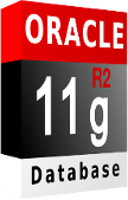
\includegraphics[scale=1]{oracle_11g}}} &
              \multicolumn{1}{c}{\textbf{
\includegraphics[scale=1]{ms_sql}}} \\
              \hline
            }
            \tablehead{
              \multicolumn{1}{c}{\textbf{Einschränkung}} &
              \multicolumn{1}{c}{\textbf{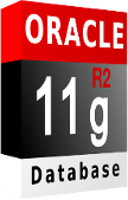
\includegraphics[scale=1]{oracle_11g}}} &
              \multicolumn{1}{c}{\textbf{
\includegraphics[scale=1]{ms_sql}}} \\
              \hline
            }
            \tabletail{
              \hline
            }
            \tablelasttail{
              \hline
            }
            \begin{supertabular}{|l|p{5.5cm}|p{5.5cm}|}
              \textbf{Bezeichnerlänge} & 30 & 128\\
              \hline
              \textbf{Reservierte Wörter} & Bezeichner können keine reservierten Wörter sein, es sei denn, sie sind in Anführungszeichen \char34{} eingeschlossen. & Bezeichner können keine reservierten Wörter sein, es sei denn, sie sind in Anführungszeichen \char34{} eingeschlossen. \\
              \hline
              \textbf{Namensgebung} & Wenn Bezeichner nicht in Anführungszeichen (\char34{}) einschlossen sind, müssen diese mit einem Buchstaben beginnen. Für umschlossene Bezeichner gilt dies nicht. & Wenn Bezeichner nicht in Anführungszeichen (\char34{}) oder ([]) einschlossen sind, müssen diese mit einem Buchstaben, \_, @ oder \# beginnen. Für umschlossene Bezeichner gilt dies nicht. \\
              \hline
              \textbf{Gültige Zeichen} & Nicht umschlossene Bezeichner können nur aus den Buchstaben a-z und A-Z, den Ziffern 0-9, sowie \_, \$ und \# bestehen. Für umschlossene Bezeichner gilt, dass dort alle Zeichen, auch Leerzeichen vorkommen können. & Nicht umschlossene Bezeichner können nur aus den Buchstaben a-z und A-Z, den Ziffern 0-9, sowie @, \$, \_ und \# bestehen. Für umschlossene Bezeichner gilt, dass dort alle Zeichen, auch Leerzeichen vorkommen können. \\
              \hline
              \textbf{Namensgleichheit} & Zwei Datenbankobjekte im gleichen Namensraum müssen unterschiedliche Namen haben.  & Bezeichner müssen innerhalb eines Schemas eindeutig sein.\\
              \hline
              \textbf{Casesensitivität} & Nicht umschlossene Bezeichner sind nicht Casesensitiv. Bezeichner die mit (\char34{}) oder ([]) umschlossen sind, sind Casesensitiv. & Bezeichner die mit (\char34{}) oder ([]) umschlossen sind, sind nicht Casesensitiv. \\
            \end{supertabular}
          \end{small}
        \end{center}
        \begin{merke}
          Damit umschlossene Bezeichner in SQL Server 2008 R2 genutzt werden können, muss die Option \textit{QUOTED\_IDENTIFIER} den Wert \textit{ON} haben. Dieser kann nötigenfalls mit \languagemssql{SET QUOTED_IDENTIFIER ON} gesetzt werden.
        \end{merke}
        Die folgenden Internetliteraturhinweise liefern weitere Informationen.

        \begin{literaturinternet}
          \item \cite{i27561}
          \item \cite{ms187879}
        \end{literaturinternet}
      \subsection{CREATE TABLE - Tabellen erstellen}
        Sowohl in Oracle als auch in SQL Server werden Tabellen mit Hilfe des
Kommandos \languageorasql{CREATE TABLE} erstellt. Die grundlegende,
SQL-Standardkonforme Syntax für \languageorasql{CREATE TABLE} lautet:
        \begin{lstlisting}[language=oracle_sql,caption={Die Syntax der CREATE TABLE-Anweisung},label=sql08_01]
CREATE TABLE <tabellen_name> (
  <spaltenbezeichner 1> <datentyp>,
  <spaltenbezeichner 2> <datentyp>,
  ...,
  <spaltenbezeichner n> <datentyp>
);
        \end{lstlisting}
        \begin{center}
          \tablecaption{Die CREATE TABLE-Anweisung}
          \label{createtablesyntax}
          \begin{small}
            \tablefirsthead{
              \multicolumn{1}{c}{\textbf{Ausdruck}} &
              \multicolumn{1}{c}{\textbf{Bedeutung}} \\
              \hline
            }
            \tablehead{
              \multicolumn{1}{c}{\textbf{Ausdruck}} &
              \multicolumn{1}{c}{\textbf{Bedeutung}} \\
              \hline
            }
            \tabletail{
              \hline
            }
            \begin{supertabular}{|l|p{9.45cm}|}
              CREATE TABLE <Tabellenname> & Diese Klausel leitet das Erstellen der Tabelle ein. Für den Tabellennamen gelten die in \tabelle{createtablerestrictions} angegebenen Beschränkungen. \\
              \hline
              <Spaltenbezeichner> <Datentyp> & Jede Tabellenspalte wird durch einen Bezeichner/Name und einen Datentyp repräsentiert. Mit Hilfe des Namens kann die Spalte später angesprochen werden und der Datentyp legt den Wertebereich der Spalte fest. Je nach DBMS gelten auch hier unterschiedliche Einschränkungen. \\
            \end{supertabular}
          \end{small}
        \end{center}
        \beispiel{sql08_02} zeigt ein einfaches \languageorasql{CREATE TABLE}-Statement.
        \begin{lstlisting}[language=oracle_sql,caption={Eine einfache CREATE TABLE-Anweisung in Oracle},label=sql08_02]
CREATE TABLE Aktie (
  Aktie_ID  NUMBER,
  Name      VARCHAR2(25),
  WKN       NUMBER,
  ISIN      VARCHAR2(12)
);
        \end{lstlisting}
        \begin{lstlisting}[language=ms_sql,caption={Das gleiche in MS SQL Server},label=sql08_03]
CREATE TABLE Aktie (
  Aktie_ID  NUMERIC,
  Name      VARCHAR(25),
  WKN       NUMERIC,
  ISIN      VARCHAR(12)
);
        \end{lstlisting}
        Es wird eine Tabelle namens \identifier{Aktie}, mit den Spalten \identifier{Aktie\_ID}, \identifier{Name}, \identifier{WKN} und \identifier{ISIN} angelegt.

        Zur besseren Umsetzung der Beispiele in den folgenden Abschnitten, werden nun einige Datensätze in die Tabelle \identifier{Aktie} eingefügt.
        \begin{lstlisting}[language=oracle_sql,caption={Beispieldatensätze},label=sql08_04]
INSERT INTO Aktie
VALUES (1, 'Henker Co KG', 1236547, 'DE0006800002');

INSERT INTO Aktie
VALUES (2, 'AD and D', 43116589, 'DE0002300023');

COMMIT;
        \end{lstlisting}
      \subsection{CREATE TABLE AS... (CTAS)}
        Die Abkürzung \enquote{CTAS} steht für \languageorasql{CREATE TABLE AS} und meint ein \languageorasql{CREATE TABLE} mit Unterabfrage. Mit Hilfe von CTAS können bestehende Tabellen teilweise oder ganz kopiert werden. \beispiel{sql08_05} zeigt, wie in Oracle eine vollständige Kopie der Tabelle \identifier{Aktie} angefertigt wird.
        \begin{lstlisting}[language=oracle_sql,caption={Oracle - CREATE TABLE AS (CTAS)},label=sql08_05]
CREATE TABLE Aktie_Kopie
AS
  SELECT *
  FROM   Aktie;
        \end{lstlisting}
          Es wird eine Tabelle namens \identifier{Aktie\_Kopie} erstellt. Diese erhält die komplette Struktur und den gesamten Inhalt der Tabelle \identifier{Aktie}.

          In Microsoft SQL Server kennt das \languagemssql{CREATE TABLE}-Statement keine Möglichkeit, eine Unterabfrage zu nutzen. Hier muss stattdessen das \languagemssql{SELECT INTO}-Statement genutzt werden.
        \begin{lstlisting}[language=ms_sql,caption={MS SQL Server - SELECT INTO},label=sql08_06]
SELECT *
INTO   Aktie_Kopie
FROM   Aktie;
        \end{lstlisting}
		\clearpage
        Die Auswirkungen bleiben die gleichen, wie unter Oracle mit CTAS.

        \begin{merke}
          Microsoft SQL Server kennt das \languagemssql{CREATE TABLE AS}-Statement nicht. Es muss stattdessen das \languagemssql{SELECT INTO}-Statement genutzt werden. Die Auswirkungen von \languagemssql{CREATE TABLE AS} und \languagemssql{SELECT INTO} sind gleich.
        \end{merke}
      \subsection{ALTER TABLE - Tabellen verändern}
        Mit Hilfe der \languageorasql{ALTER TABLE}-Anweisung können bestehende Tabellendefinition verändert werden. Dies betrifft z. B.:
        \begin{itemize}
          \item Das Hinzufügen neuer Spalten zu einer Tabelle.
          \item Das Löschen von Spalten.
          \item Das Umbenennen von Spalten.
          \item Das Ändern des Datentyps einer Spalte.
          \item Ändern der Größe einer Spalte.
          \item Das Hinzufügen, ändern und löschen eines Standardwerts.
          \item Das Hinzufügen und Löschen von Constraints (siehe \abschnitt{constraints1})
        \end{itemize}
		\clearpage
        \subsubsection{Eine neue Spalte an eine Tabelle anfügen}
          In beiden DBMS gibt es, zum Hinzufügen einer Spalte zu einer Tabelle, die \lstinline{ADD}-Klausel des \languageorasql{ALTER TABLE}-Kommandos. In \beispiel{sql08_07}, wird der Tabelle \identifier{Aktie} eine neue Spalte namens \identifier{Herkunft} hinzugefügt.
          \begin{lstlisting}[language=oracle_sql,caption={Oracle - Tabellenspalte hinzufügen},label=sql08_07]
ALTER TABLE Aktie
ADD Herkunft VARCHAR2(25);
          \end{lstlisting}
          In SQL Server unterscheidet sich dieses Statement nur durch den Datentyp.
          \begin{lstlisting}[language=ms_sql,caption={MS SQL Server - Tabellenspalte hinzufügen},label=sql08_08]
ALTER TABLE Aktie
ADD Herkunft VARCHAR(25);
          \end{lstlisting}
          \begin{merke}
            Wird eine neue Spalte an eine Tabelle angefügt, haben alle Zellen dieser Spalte den Wert NULL, es sei den, es wird ein Standardwert für diese Spalte definert. In diesem Falle füllt Oracle die Spalte mit dem Standardwert auf. SQL Server tut dies nicht.
          \end{merke}
           \beispiel{sql08_09} und \beispiel{sql08_10} zeigen, wie sich Oracle und MS SQL Server verhalten, wenn eine neue Spalte, mit einem Standardwert, hinzugefügt wird. Die Spalte \identifier{Herkunft} wird mit dem Standardwert \enquote{Deutschland} an die Tabelle \identifier{Aktie} angefügt. In Oracle werden dann automatisch alle bereits vorhandenen Zeilen mit dem neuen Standardwert aufgefüllt. In SQL Server wird dies nicht der Fall sein.
          \begin{lstlisting}[language=oracle_sql,caption={Tabellenspalte mit Standardwert hinzufügen in Oracle},label=sql08_09]
ALTER TABLE Aktie
ADD Herkunft VARCHAR2(25) DEFAULT 'Deutschland';

SELECT *
FROM   Aktie;
          \end{lstlisting}
          \begin{center}
            \begin{small}
              \changefont{pcr}{m}{n}
              \tablefirsthead {
                \multicolumn{1}{r}{\textbf{AKTIE\_ID}} &
                \multicolumn{1}{l}{\textbf{NAME}} &
                \multicolumn{1}{l}{\textbf{WKN}} &
                \multicolumn{1}{l}{\textbf{ISIN}} &
                \multicolumn{1}{l}{\textbf{HERKUNFT}} \\
                \cmidrule(r){1-1}\cmidrule(l){2-2}\cmidrule(l){3-3}\cmidrule(l){4-4}\cmidrule(l){5-5}
              }
              \tablehead{}
              \tabletail {
                \multicolumn{5}{l}{\textbf{2 Zeilen ausgewählt}} \\
              }
              \tablelasttail {
                \multicolumn{5}{l}{\textbf{2 Zeilen ausgewählt}} \\
              }
              \begin{oraclesql}
                \begin{supertabular}{rllll}
                  1 & Henker Co KG & 1236547 & DE0006800002 & Deutschland \\
                  2 & AD and D & 43116589 & DE0002300023 & Deutschland \\
                \end{supertabular}
              \end{oraclesql}
            \end{small}
          \end{center}

          Wird das gleiche Experiment in MS SQL Server durchgeführt, zeigt sich das die Spalte \identifier{Herkunft} nicht automatisch aufgefüllt wird.
          \begin{lstlisting}[language=ms_sql,caption={Tabellenspalte mit Standardwert hinzufügen in SQL Server},label=sql08_10]
ALTER TABLE Aktie
ADD Herkunft VARCHAR(25) DEFAULT 'Deutschland';

SELECT *
FROM   Aktie;
          \end{lstlisting}
          \begin{center}
            \begin{small}
              \changefont{pcr}{m}{n}
              \tablefirsthead {
                \multicolumn{1}{l}{\textbf{AKTIE\_ID}} &
                \multicolumn{1}{l}{\textbf{NAME}} &
                \multicolumn{1}{l}{\textbf{WKN}} &
                \multicolumn{1}{l}{\textbf{ISIN}} &
                \multicolumn{1}{l}{\textbf{HERKUNFT}} \\
                \cmidrule(l){1-1}\cmidrule(l){2-2}\cmidrule(l){3-3}\cmidrule(l){4-4}\cmidrule(l){5-5}
              }
              \tablehead{}
              \tabletail {
                \multicolumn{5}{l}{\textbf{2 Zeilen ausgewählt}} \\
              }
              \tablelasttail {
                \multicolumn{5}{l}{\textbf{2 Zeilen ausgewählt}} \\
              }
              \begin{oraclesql}
                \begin{supertabular}{lllll}
                  1 & Henker Co KG & 1236547 & DE0006800002 &  NULL \\
                  2 & AD and D & 43116589 & DE0002300023 & NULL \\
                \end{supertabular}
              \end{oraclesql}
            \end{small}
          \end{center}
        \subsubsection{Spalten vergrößern und verkleinern}
          Es besteht die Möglichkeit, die Definition einer Spalte nachträglich zu verändern. Dabei können verschiedene Dinge, wie z. B. der Spaltendatentyp oder der Standardwert einer Spalte geändert werden. Um eine solche Änderung durchzuführen, kennt das \languageorasql{ALTER TABLE}-Kommando unter Oracle die \languageorasql{MODIFY}-Klausel und unter SQL Server die \languagemssql{ALTER COLUMN}-Klausel. Hierzu einige Beispiele.

          In \beispiel{sql08_11} wird die Breite der Spalte \identifier{Herkunft} in der Tabelle \identifier{Aktie} verändert.
          \begin{lstlisting}[language=oracle_sql,caption={Anpassen der Spaltenlänge in Oracle},label=sql08_11]
ALTER TABLE Aktie
MODIFY Herkunft VARCHAR2(30);
          \end{lstlisting}
\clearpage
          Eine Vergrößerung stellt prinzipiell niemals ein Problem dar. Schwieriger wird es hingegen, wenn eine Spalte verkleinert werden muss. In Oracle geht das nur dann, wenn die Inhalte der Spalte kleiner sind als die neue Spaltengröße. Anderenfalls antwortet Oracle mit der in \beispiel{sql08_12} sichtbaren Fehlermeldung:
          \begin{lstlisting}[language=oracle_sql,caption={Fehlermeldung beim verkleinern einer Spalte in Oracle},label=sql08_12]
MODIFY Herkunft VARCHAR2(15)
       *
FEHLER in Zeile 2:
ORA-01441: Spaltenlaenge kann nicht vermindert werden, weil ein Wert zu gross
ist
          \end{lstlisting}
          \begin{merke}
            Eine Tabellenspalte kann in Oracle nur auf die Größe des größten darin enthaltenden Werts verkleinert werden. In SQL Server kann eine Tabellenspalte auch mit Inhalt verkleinert werden.
          \end{merke}
          Bei SQL Server muss lediglich die \languageorasql{MODIFY}-Klausel durch die \languagemssql{ALTER COLUMN}-Klausel ersetzt werden.
          \begin{lstlisting}[language=ms_sql,caption={Anpassen der Spaltenlänge in SQL Server},label=sql08_13]
ALTER TABLE Aktie
ALTER COLUMN Herkunft VARCHAR(30);
          \end{lstlisting}
        \subsubsection{Ändern des Datentyps}
          Mit Hilfe der \languageorasql{MODIFY}-Klausel kann nicht nur die Größe einer Spalte verändert werden, sondern auch der Datentyp. In \beispiel{sql08_14} wird der Datentyp der Spalte \identifier{WKN} von \languageorasql{NUMBER} auf \languageorasql{VARCHAR2}, bzw. von \languagemssql{NUMERIC} auf \languagemssql{VARCHAR} geändert.
          \begin{lstlisting}[language=oracle_sql,caption={Ändern des Datentyps},label=sql08_14]
ALTER TABLE Aktie
MODIFY WKN VARCHAR2(10);
          \end{lstlisting}
          In SQL Server sieht das Ändern des Datentyps einer Spalte sehr ähnlich aus.
          \begin{lstlisting}[language=ms_sql,caption={Ändern des Datentyps},label=sql08_15]
ALTER TABLE Aktie
ALTER COLUMN WKN VARCHAR(10);
          \end{lstlisting}
          \begin{merke}
            Eine Tabellenspalte muss in Oracle leer sein, damit ihr Datentyp verändert werden kann. In SQL Server kann der Datentyp einer Spalte auch mit Inhalt verändert werden.
          \end{merke}
\clearpage
        \subsubsection{Einen Defaultvalue hinzufügen}
          Eine weitere Aktion die mit \languageorasql{MODIFY} bzw. \languagemssql{ALTER COLUMN} möglich ist, ist das Hinzufügen, ändern oder entfernen eines Standardwertes bei einer Tabellenspalte. In \beispiel{sql08_16} wird in Oracle der Standardwert der Spalte \identifier{Herkunft} von \enquote{Deutschland} auf \enquote{USA} geändert.
          \begin{lstlisting}[language=oracle_sql,caption={Einen Standardwert ändern},label=sql08_16]
ALTER TABLE Aktie
MODIFY Herkunft DEFAULT 'USA';
          \end{lstlisting}
          Mit der gleichen Anweisung kann der Standardwert eine Spalte, unter Oracle, nicht nur geändert sondern auch hinzugefügt werden. Das Löschen des Standardwertes geschieht, indem NULL als Standardwert zugewiesen wird.
          \begin{lstlisting}[language=oracle_sql,caption={Standardwert hinzufügen},label=sql08_17]
ALTER TABLE Aktie
MODIFY Herkunft DEFAULT NULL;
          \end{lstlisting}
          Bei SQL Server ist das Löschen eines Standardwerts anders als bei
          Oracle. In SQL Server wird ein Standardwert als sogenanntes
          Constraint\footnote{constraint engl. = Einschränkung} gehandhabt.
          Deshalb wird diese Aktion zu einem späteren Zeitpunkt in
          \abschnitt{sqlserverdefaultconstraint} behandelt.

          \begin{merke}
            Wird in Oracle mit Hilfe \languageorasql{ADD}-Klausel eine Spalte
            mit Standardwert hinzugeügt, werden alle NULL-Werte in der
            gleichen Spalte mit dem Standardwert aufgefüllt. Wird die Spalte
            dagegen mit der \languageorasql{MODIFY}-Klausel, nachträglich mit
            einem Default-Wert ausgestattet, bleiben alle NULL-Werte erhalten!
          \end{merke}

				\subsubsection{Tabellenspalten umbenennen}
          Es ist möglich, bestehende Spalten umzubenennen. Dafür wird in
          Oracle die \languageorasql{RENAME COLUMN}-Klausel des
          \languageorasql{ALTER TABLE}-Kommandos verwendet. In Microsoft SQL
          Server gibt es hierfür eine gespeicherte Hilfsprozedur, welche das
          Umbenennen übernimmt. Der neue Spaltenname muss innerhalb der
          Tabelle eindeutig sein und es dürfen keine anderen Operationen
          zusammen mit dem Umbenennen geschehen.
          \begin{lstlisting}[language=oracle_sql,caption={Tabellenspalte umbenennen in Oracle},label=sql08_18]
ALTER TABLE Aktie
RENAME COLUMN Name TO Bezeichnung;
          \end{lstlisting}
          \begin{lstlisting}[language=ms_sql,caption={Tabellenspalte umbenennen in SQL Server},label=sql08_19, emphstyle={[9]\color{red}},emph={[9]sp_rename}]
EXEC sp_rename 'Aktie.Name', 'Bezeichnung', 'COLUMN'
          \end{lstlisting}
          \begin{merke}
            Für das Umbenennen von Objekten ist in SQL Server die gespeicherte
            Hilfsprozedur \languagemssql{sp\_rename} zuständig.
          \end{merke}
          Zu beachten ist, dass das Umbenennen einer Spalte Auswirkungen auf
          abhängige Objekte wie z. B. Views oder Trigger haben kann und
          deshalb mit größter Vorsicht durchzuführen ist.
        \subsubsection{Tabellenspalten löschen}
          Tabellenspalten, die nicht mehr benötigt werden, können jeder
          Zeit gelöscht werden. Auf diese einfache Art und Weise kann
          Speicherplatz zu weiteren Nutzung freigegeben werden. Allgemein gilt
          als Einschränkung beim Löschen einer Tabellenspalte:
          \begin{itemize}
            \item Die letzte Spalte in einer Tabelle kann nicht gelöscht
            werden. Es muss dann die gesamte Tabelle gelöscht werden.
          \end{itemize}
          Für Oracle gilt zusätzlich:
          \begin{itemize}
            \item Ein normaler Nutzer kann keine Spalten aus einer Tabelle
            löschen, die dem Nutzer sys gehört.
          \end{itemize}
          \beispiel{sql08_19} zeigt das Löschen einer Tabellenspalte in Oracle und SQL Server.
          \begin{lstlisting}[language=oracle_sql, caption={Tabellenspalte
          löschen},label=sql08_20]
ALTER TABLE Aktie
DROP COLUMN WKN;
          \end{lstlisting}
      \subsection{DROP TABLE - Tabellen löschen}
        Eine nicht mehr benötigte Tabelle, wird in Oracle und SQL Server mit dem \languageorasql{DROP TABLE}-Kommando gelöscht.
        \begin{itemize}
          \item Alle verknüpften Indizes und Trigger werden mitgelöscht.
          \item Alle abhängigen Views bleiben bestehen und werden ungültig.
        \end{itemize}
        Das folgende Beispiel löscht die Tabelle \identifier{Aktie}.
        \begin{lstlisting}[language=oracle_sql,caption={Eine Tabelle löschen},label=sql08_21]
DROP TABLE Aktie;
        \end{lstlisting}
      \subsection{TRUNCATE TABLE - Tabellen leeren}
        Eine Tabelle kann mit \languageorasql{TRUNCATE TABLE} geleert werden. Die Tabelle selbst bleibt dabei erhalten. Um eine Tabelle zu leeren, gibt es drei Möglichkeiten:
        \begin{itemize}
          \item Das DML-Statement \languageorasql{DELETE}
          \item Das Löschen der Tabelle mit \languageorasql{DROP TABLE} und neu erstellen mit \languageorasql{CREATE TABLE}
          \item Das DDL-Statement \languageorasql{TRUNCATE}
        \end{itemize}
        \subsubsection{Den Tabelleninhalt mit DELETE löschen}
          Es können alle Zeilen einer Tabelle mit dem DML-Kommando \languageorasql{DELETE} gelöscht werden.
          \begin{lstlisting}[language=oracle_sql,caption={Zeilen mit DELETE löschen},label=sql08_22]
DELETE FROM Aktie;
          \end{lstlisting}
          Bei einer großen Tabelle werden hierfür sehr viele
          Systemressourcen benötigt (CPU, RAM, usw.). Des Weiteren kann es
          passieren, dass beim Löschen von Zeilen, Trigger ausgelöst werden.

          \begin{merke}
            Der Speicherplatz, der durch die Tabelle vor dem Löschen belegt
            wurde, bleibt bei der Verwendung von \languageorasql{DELETE} belegt.
          \end{merke}
          Einziger Vorteil ist, dass mit der \languageorasql{DELETE}-Klausel die
          Zeilen ausgewählt werden können, die gelöscht werden sollen.
        \subsubsection{Die Tabelle löschen und neu erstellen}
          \label{dropandrecreatetable}
          Eine Tabelle kann gelöscht und mit \languageorasql{CREATE TABLE} neu
          erstellt werden. Dabei gehen alle mit dieser Tabelle verbundenen
          Indizes, Integritäts Constraints und Trigger verloren und alle von
          der Tabelle abhängigen Objekte werden ungültig.
        \subsubsection{Eine Tabelle mit TRUNCATE leeren}
          Um alle Zeilen einer Tabelle zu löschen kann das \languageorasql{TRUNCATE}-Statement verwendet werden.
          \begin{lstlisting}[language=oracle_sql, caption={Zeilen mit TRUNCATE
          abschneiden},label=sql08_23]
TRUNCATE TABLE Aktie;
          \end{lstlisting}
          \begin{merke}
            In Oracle produziert das \languageorasql{TRUNCATE}-Statement, wie
            alle DDL-Statements, automatisch ein \languageorasql{COMMIT}, d. h.
            es kann nicht rückgängig gemacht werden. In SQL Server ist das
            Zurückrollen eines \languagemssql{TRUNCATE}-Statements möglich.
          \end{merke}

          \begin{merke}
            Der Speicherplatz, der durch die Tabelle vor dem Löschen belegt
            wurde, wird bei der Verwendung von \languageorasql{TRUNCATE},
            freigegeben.
          \end{merke}
    \section{Views erstellen verwalten}
      \subsection{Was sind Views?}
        Bei der täglichen Arbeit mit einer Datenbank treten häufig immer wiederkehrende \SELECT-Statements auf. Dies kann z. B. deshalb sein, weil ein Nutzer immer wieder die gleiche Sicht (gleiche Spalten, gleiche Filterbedingung) auf die Daten einer Tabelle benötigt.

        \begin{merke}
          Eine View ist eine genau definierte Sicht auf eine bestimmte Datenmenge.
        \end{merke}
      \subsection{Views erstellen}
        Views werden mit dem \languageorasql{CREATE VIEW}-Kommando erstellt. Die Syntax für \languageorasql{CREATE VIEW} sieht wie folgt aus:
        \begin{lstlisting}[language=oracle_sql,caption={Die Syntax von CREATE VIEW},label=sql08_24]
CREATE VIEW <View_name>
(<Spalten_alias 1, Spalten_alias 2, ..., Spalten_alias n)
AS
  <Auswahlabfrage>;
        \end{lstlisting}
        \begin{center}
          \tablecaption{Die CREATE VIEW-Anweisung}
          \label{createviewsyntax}
          \begin{small}
            \tablefirsthead{
              \multicolumn{1}{c}{\textbf{Ausdruck}} &
              \multicolumn{1}{c}{\textbf{Bedeutung}} \\
              \hline
            }
            \tablehead{
              \multicolumn{1}{c}{\textbf{Ausdruck}} &
              \multicolumn{1}{c}{\textbf{Bedeutung}} \\
              \hline
            }
            \tabletail{
              \hline
            }
            \tablelasttail{
              \hline
            }
            \begin{supertabular}{|l|p{9.45cm}|}
              CREATE VIEW <View\_name> & Diese Klausel leitet das Erstellen der View ein. Für den Viewname gelten die in \tabelle{createtablerestrictions} angegebenen Beschränkungen. \\
              \hline
              <Spalten\_alias> & Für jeden Spaltenbezeichner, der in der Auswahlabfrage genutzt wird, kann an dieser Stelle ein Aliasname festgelegt werden.\\
              \hline
              <Auswahlabfrage> & Dies ist das SELECT-Statement. \\
            \end{supertabular}
          \end{small}
        \end{center}
        Ein einfaches Beispiel für das Erstellen einer View ist in \beispiel{sql08_24} zu sehen.
        \begin{lstlisting}[language=oracle_sql,caption={Eine einfache View},label=sql08_25]
CREATE VIEW v_Kunde
AS
  SELECT Vorname, Nachname
  FROM   Kunde;
        \end{lstlisting}
		\clearpage
        Was an dieser Stelle passiert ist, dass das DBMS das \SELECT-Statement verarbeitet und unter dem Namen \identifier{v\_Kunden} abspeichert. Anschließend kann, wie in \beispiel{sql08_26}, mit SQL auf die View zugegriffen werden.
        \begin{lstlisting}[language=oracle_sql,caption={Zugriff auf eine View},label=sql08_26]
SELECT Vorname, Nachname
FROM   v_Kunde;
        \end{lstlisting}
        \begin{center}
          \begin{small}
            \changefont{pcr}{m}{n}
            \tablefirsthead {
              \multicolumn{1}{l}{\textbf{VORNAME}} &
              \multicolumn{1}{l}{\textbf{NACHNAME}} \\
              \cmidrule(l){1-1}\cmidrule(l){2-2}
            }
            \tablehead{}
            \tabletail {
              \multicolumn{2}{l}{\textbf{561 Zeilen ausgewählt}} \\
            }
            \tablelasttail {
              \multicolumn{2}{l}{\textbf{561 Zeilen ausgewählt}} \\
            }
            \begin{msoraclesql}
              \begin{supertabular}{ll}
                Niklas & Schneider \\
                Mia & Keller \\
                Lilli & Beck \\
                Emilia & Keller \\
                Finn & Junge \\
                Marie & Vogel \\
                Rudi & Roggatz \\
                Leni & Koch \\
                Chris & Zimmermann \\
                Justin & Gabriel \\
                Sebastian & Schröder \\
              \end{supertabular}
            \end{msoraclesql}
          \end{small}
        \end{center}
        Auch wenn in der \SELECT-Klausel der Auswahlabfrage der * verwendet wird, wird im Hintergrund folgendes Statement, als View gespeichert:
        \begin{lstlisting}[language=oracle_sql,caption={Was tatsächlich gespeichert wird},label=sql08_27]
-- So wird die View erstellt
CREATE VIEW v_Kunde
AS
  SELECT *
  FROM   Kunde;

-- Das wird gespeichert
SELECT Kunden_ID, Vorname, Nachname
FROM   Kunde;
        \end{lstlisting}
		\clearpage
        Diese Tatsache ist nicht ganz unwichtig, wie folgendes Szenario beweist:
        \begin{lstlisting}[language=oracle_sql,caption={Eine Szenario mit Tücke},label=sql08_28]
CREATE VIEW v_Aktie
AS
  SELECT *
  FROM   Aktie;

ALTER TABLE Aktie
ADD Herkunft VARCHAR2(30);

SELECT *
FROM   v_Aktie;
        \end{lstlisting}
        \begin{center}
          \begin{small}
            \changefont{pcr}{m}{n}
            \tablefirsthead {
              \multicolumn{1}{r}{\textbf{AKTIE\_ID}} &
              \multicolumn{1}{l}{\textbf{NAME}} &
              \multicolumn{1}{l}{\textbf{WKN}} &
              \multicolumn{1}{l}{\textbf{ISIN}} \\
              \cmidrule(r){1-1}\cmidrule(l){2-2}\cmidrule(l){3-3}\cmidrule(l){4-4}
            }
            \tablehead{}
            \tabletail {
              \multicolumn{5}{l}{\textbf{2 Zeilen ausgewählt}} \\
            }
            \tablelasttail {
              \multicolumn{5}{l}{\textbf{2 Zeilen ausgewählt}} \\
            }
            \begin{msoraclesql}
              \begin{supertabular}{rllll}
                1 & Henker Co KG & 1236547 & DE0006800002  \\
                2 & AD and D & 43116589 & DE0002300023  \\
              \end{supertabular}
            \end{msoraclesql}
          \end{small}
        \end{center}
        Da bei der Erstellung der View \identifier{v\_Aktie}, der *, in die einzelnen Spalten der Tabelle \identifier{Aktie} aufgelöst wurde, ist die neu hinzugefügte Spalte \identifier{Herkunft}, in der View \identifier{v\_Aktie} noch nicht zu sehen. Hierzu müsste die Viewdefinition geändert bzw. die View neu erstellt werden.

        \begin{merke}
          Wird in der Auswahlabfrage einer View das * Symbol verwendet, wird dieses interpretiert. D. h. es wird ersetzt durch die tatsächliche Spaltenliste der Quelltabelle. Änderungen an der Struktur der Tabelle werden somit von der View nicht erkannt.
        \end{merke}
        Wie in \tabelle{createviewsyntax} bereits erklärt, kann bei der Erstellung einer View auch eine Liste mit Spaltenaliasnamen angegeben werden. Dies ist in den folgenden Fällen immer notwendig:
        \begin{itemize}
          \item Wenn in der View ein berechneter Ausdruck vorhanden ist
          \item Wenn in der View mehrere Tabellen mit einem Join verbunden sind und Spalten mit gleichem Namen ausgegeben werden müssen.
        \end{itemize}
		\clearpage
        \beispiel{sql08_29} zeigt eine View mit Spaltenaliasliste.
        \begin{lstlisting}[language=oracle_sql,caption={Eine einfache View mit Spaltenaliasliste},label=sql08_29]
CREATE VIEW v_Kunde
(Vorname, Nachname, Lebensalter)
AS
SELECT k.Vorname, k.Nachname,
       ROUND(MONTHS_BETWEEN(SYSDATE, Geburtsdatum) / 12, 0)
FROM   Kunde k INNER JOIN Eigenkunde ek
       ON (k.Kunden_ID = ek.Kunden_ID);

SELECT *
FROM   v_Kunde;
        \end{lstlisting}
        \begin{center}
          \begin{small}
            \changefont{pcr}{m}{n}
            \tablefirsthead {
              \multicolumn{1}{l}{\textbf{VORNAME}} &
              \multicolumn{1}{l}{\textbf{NACHNAME}} &
              \multicolumn{1}{r}{\textbf{LEBENSALTER}} \\
              \cmidrule(l){1-1}\cmidrule(l){2-2}\cmidrule(r){3-3}
            }
            \tablehead{}
            \tabletail {
              \multicolumn{3}{l}{\textbf{400 Zeilen ausgewählt}} \\
            }
            \tablelasttail {
              \multicolumn{3}{l}{\textbf{400 Zeilen ausgewählt}} \\
            }

            \begin{oraclesql}
              \begin{supertabular}{llr}
                Mia & Keller & 41 \\
                Emilia & Keller & 23 \\
                Finn & Junge & 37 \\
                Marie & Vogel & 42 \\
                Rudi & Roggatz & 26 \\
                Leni & Koch & 38 \\
                Chris & Zimmermann & 23 \\
                Sebastian & Schröder & 24 \\
                Justin & Zimmermann & 34 \\
                Petra & Krause & 34 \\
                Clara & Rollert & 23 \\
                Gustav & Witte & 23 \\
              \end{supertabular}
            \end{oraclesql}
          \end{small}
        \end{center}
        Wie gut zu erkennen ist, ersetzen die Spaltenaliase die tatsächlichen Spaltennamen in \identifier{v\_Kunde}. Die gleiche Auswirkung wäre auch mit dem folgenden Statement zu erreichen:
        \begin{lstlisting}[language=oracle_sql,caption={Eine einfache View mit Spaltenaliasen},label=sql08_30]
CREATE VIEW v_Kunde
AS
SELECT k.Vorname, k.Nachname,
       ROUND(MONTHS_BETWEEN(SYSDATE, Geburtsdatum) / 12, 0) AS Lebensalter
FROM   Kunde k INNER JOIN Eigenkunde ek
       ON (k.Kunden_ID = ek.Kunden_ID);
        \end{lstlisting}
        \begin{merke}
          Wird eine Spaltenaliasliste genutzt, muss diese genauso viele Aliasnamen umfassen, wie die \SELECT-Liste der Auswahlabfrage Spaltennamen zurückgibt.
        \end{merke}
        Hierzu ein kleines Beispiel. Im folgenden \languageorasql{CREATE VIEW}-Statement werden zu wenige Spaltenaliase angegeben. Oracle und auch SQL Server antworten prompt mit einer Fehlermeldung.
        \begin{lstlisting}[language=oracle_sql,caption={Eine einfache View mit fehlerhafter Spaltenaliasliste in Oracle},label=sql08_31]
CREATE VIEW v_Kunde
(Vorname, Nachname)
AS
SELECT k.Vorname, k.Nachname,
       ROUND(MONTHS_BETWEEN(SYSDATE, Geburtsdatum) / 12, 0)
FROM   Kunde k INNER JOIN Eigenkunde ek
       ON (k.Kunden_ID = ek.Kunden_ID);

(Vorname, Nachname)
 *
FEHLER in Zeile 2:
ORA-01730: invalid number of column names specified
        \end{lstlisting}
        SQL Server antwortet wie folgt:
        \begin{lstlisting}[language=ms_sql,caption={Eine einfache View mit fehlerhafter Spaltenaliasliste in SQL Server},label=sql08_32]
CREATE VIEW v_Kunde
(Vorname, Nachname)
AS
SELECT k.Vorname, k.Nachname, DATEDIFF(YEAR, getDate(), Geburtsdatum)
FROM   Kunde k INNER JOIN Eigenkunde ek
       ON (k.Kunden_ID = ek.Kunden_ID);

Meldung 8158, Ebene 16, Status 1, Prozedur v_Kunde, Zeile 4
'v_Kunde' besitzt mehr Spalten, als in der Spaltenliste angegeben sind.
        \end{lstlisting}
        Bereits weiter oben in diesem Abschnitt wurde erläutert, dass eine View, in der ein berechneter Ausdruck vorkommt, zwingend mit Spaltenaliasen versehen werden muss. \beispiel{sql08_33} beweist dies:
        \begin{lstlisting}[language=oracle_sql,caption={Eine View mit einer berechneten Spalte in Oracle},label=sql08_33]
CREATE VIEW v_Kunde
(Vorname, Nachname)
AS
SELECT k.Vorname, k.Nachname,
       ROUND(MONTHS_BETWEEN(SYSDATE, Geburtsdatum) / 12, 0)
FROM   Kunde k INNER JOIN Eigenkunde ek
       ON (k.Kunden_ID = ek.Kunden_ID);

SELECT k.Vorname, k.Nachname,
ROUND(MONTHS_BETWEEN(SYSDATE, Geburtsdatum) / 12, 0)
                                   *
FEHLER in Zeile 3:
ORA-00998: Dieser Ausdruck braucht einen Spalten-Alias
        \end{lstlisting}
\clearpage
        Auch SQL Server hat hiermit Probleme:
        \begin{lstlisting}[language=ms_sql,caption={Eine View mit einer berechneten Spalte in SQL Server},label=sql08_34]
CREATE VIEW v_Kunde (Vorname, Nachname)
AS
SELECT k.Vorname, k.Nachname, DATEDIFF(YEAR, getDate(), Geburtsdatum)
FROM   Kunde k INNER JOIN Eigenkunde ek ON (k.Kunden_ID = ek.Kunden_ID);

Meldung 4511, Ebene 16, Status 1, Prozedur v_Kunde, Zeile 3
Fehler beim Ausf&ü&hren von CREATE VIEW oder CREATE FUNCTION, da
f&ü&r die 3-Spalte kein Spaltenname angegeben wurde.
        \end{lstlisting}
        Dieses Problem kann durch eine Spaltenaliasliste oder durch die direkte Vergabe eines Spaltenalias gelöst werden.

        \begin{merke}
          Bei SQL Server gibt es noch die Einschränkung, dass die Auswahlabfrage einer View keine \ORDERBY-Klausel enthalten darf.
        \end{merke}
		\clearpage
      \subsection{Views und DML}
        Views können  auch für die Ausführung von DML-Statements verwendet werden. Dabei gibt es jedoch einige Einschränkungen und Regeln die zu beachten sind.
        \begin{center}
          \tablecaption{Regeln für DML-Operationen auf Views}
          \label{rulesdmlviews}
          \begin{small}
            \tablefirsthead{
              \multicolumn{1}{c}{} &
              \multicolumn{1}{c}{\textbf{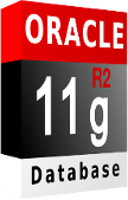
\includegraphics[scale=1]{oracle_11g}}} &
              \multicolumn{1}{c}{\textbf{
\includegraphics[scale=1]{ms_sql}}} &
              \multicolumn{1}{c}{\textbf{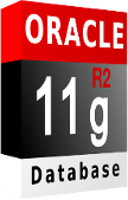
\includegraphics[scale=1]{oracle_11g}}} &
              \multicolumn{1}{c}{\textbf{
\includegraphics[scale=1]{ms_sql}}} &
              \multicolumn{1}{c}{\textbf{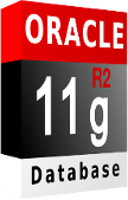
\includegraphics[scale=1]{oracle_11g}}} &
              \multicolumn{1}{c}{\textbf{
\includegraphics[scale=1]{ms_sql}}} \\
              \multicolumn{1}{c}{Einschränkung} &
              \multicolumn{2}{c}{INSERT} &
              \multicolumn{2}{c}{UPDATE} &
              \multicolumn{2}{c}{DELETE} \\
              \hline
            }
            \tabletail{
              \hline
            }
            \tablelasttail {
              \hline
            }
            \begin{supertabular}{|p{8.5cm}|c|c|c|c|c|c|}
              Es dürfen keine Aggregatfunktionen (COUNT, SUM, MAX, MIN, AVG) in der View genutzt werden. & X & X & X & X & X & X \\
              \hline
              Die View darf keine GROUP BY-Klausel enthalten. & X & X & X & X & X & X \\
              \hline
              Die View darf das DISTINCT-Schlüsselwort nicht benutzen. & X & X & X & X & X & X\\
              \hline
              Die View darf keine berechneten Ausdrücke aufweisen. & X & X & X & X & & \\
              \hline
              Die View darf keine Pseudospalten enthalten & X & & X & & X & \\
              \hline
              Die View darf keinen Join enthalten. & X & X & & & X & X \\
              \hline
              Alle mit NOT NULL markierten Spalten der Basistabelle müssen im INSERT-Statement berücksichtigt werden. & X & X & & & & \\
              \hline
              Der Einfüge- bzw. Änderungsvorgang muss, falls eine CHECK-Option in der View vorhanden ist (siehe \abschnitt{CHECK}), den Vorgaben der WHERE-Klausel der Abfrage genügen. & X & X & X & X & & \\
              \hline
              Die View darf keine READ ONLY-Option (siehe \abschnitt{READONLY}) enthalten. & X & & X & & &\\
            \end{supertabular}
          \end{small}
        \end{center}
		\clearpage
        \subsubsection{Die Einschränkung WITH CHECK OPTION}
          \label{CHECK}
          Bei der Erstellung einer View kann eine zusätzliche Einschränkung mit angegeben werden, die \languageorasql{CHECK OPTION}. Diese schränkt den Nutzer dahingehend ein, dass nur noch solche Datensätze geändert werden können, die auch in der View zu sehen sind.
          \begin{lstlisting}[language=oracle_sql,caption={Ein Experiment mit den CHECK OPTION},label=sql08_35]
CREATE VIEW v_Mitarbeiter
AS
  SELECT *
  FROM   Mitarbeiter
  WHERE  Bankfiliale_ID = 5;

INSERT INTO v_Mitarbeiter
VALUES (666, 'Florian', 'Weidinger', 12, 8,
        TO_DATE('01.03.1988', 'DD.MM.YYYY'),
        '38B546C1-CDF-36A7B97', 1500, 'Abendrot Gase',
        '13', '39444', 'Hecklingen', 20);

1 row inserted

ROLLBACK;
          \end{lstlisting}
          Obwohl die \WHERE-Klausel der View \identifier{v\_Mitarbeiter} die Anzeige auf die Bankfiliale mit der ID fünf einschränkt, kann trotzdem ein Datensatz in die Bankfiliale Nummer acht eingefügt werden.
		  
          Um die DML-Möglichkeiten der View \identifier{v\_Mitarbeiter} einzuschränken, wird im nächsten Beispiel die \languageorasql{CHECK}-Option angewendet.
          \begin{lstlisting}[language=oracle_sql,caption={Ein Experiment mit der CHECK OPTION in Oracle},label=sql08_36]
CREATE VIEW v_Mitarbeiter
AS
  SELECT *
  FROM   Mitarbeiter
  WHERE  Bankfiliale_ID = 5
WITH CHECK OPTION;

INSERT INTO v_Mitarbeiter
VALUES (666, 'Florian', 'Weidinger', 12, 8,
        TO_DATE('01.03.1988', 'DD.MM.YYYY'),
        '38B546C1-CDF-36A7B97', 1500, 'Abendrot Gase',
        '13', '39444', 'Hecklingen', 20);

INSERT INTO v_Mitarbeiter
         *
FEHLER in Zeile 1:
ORA-01402: Verletzung der where-Klausel einer View with check option
          \end{lstlisting}
          Da jetzt die \languageorasql{CHECK}-Option genutzt wurde, reagiert das DBMS mit einer Fehlermeldung auf DML-Statements, die sich auf \identifier{v\_Mitarbeiter} beziehen und nicht der \WHERE-Klausel der View entsprechen.
          \begin{lstlisting}[language=ms_sql,caption={Ein Experiment mit der CHECK OPTION in SQL Server},label=sql08_37]
CREATE VIEW v_Mitarbeiter
AS
  SELECT *
  FROM   Mitarbeiter
  WHERE  Bankfiliale_ID = 5
WITH CHECK OPTION;

INSERT INTO v_Mitarbeiter
VALUES (666, 'Florian', 'Weidinger', 12, 8,
        CONVERT(DATETIME2, '01.03.1988', 104),
        '38B546C1-CDF-36A7B97', 1500, 'Abendrot Gase',
        '13', '39444', 'Hecklingen', 20);

Meldung 550, Ebene 16, Status 1, Zeile 1
Fehler beim Einf&ü&gen oder Aktualisieren, da die Zielsicht WITH CHECK OPTION
angibt oder sich auf eine Sicht erstreckt, die WITH CHECK OPTION angibt,
und mindestens eine Ergebniszeile nicht der CHECK OPTION-Einschr&ä&nkung
entsprach.
          \end{lstlisting}
        \subsubsection{Die Einschränkung WITH READ ONLY - Oracle}
          \label{READONLY}
          Die \languageorasql{READ ONLY}-Option für Views ermöglicht es, einem Nutzer den Schreibzugriff auf eine View zu verbieten. Die View kann somit nur noch lesend genutzt werden.
          \begin{lstlisting}[language=oracle_sql,caption={Eine View mit mit READ ONLY Option erstellen},label=sql08_38]
CREATE VIEW v_Mitarbeiter
AS
  SELECT *
  FROM   Mitarbeiter
WITH READ ONLY;
          \end{lstlisting}
          Versucht ein Nutzer trotzdem mit einem DML-Statement auf die View zuzugreifen, wird er mit einer Fehlermeldung abgewiesen.
\clearpage
          \begin{lstlisting}[language=oracle_sql,caption={Daten in eine READ ONLY View einfügen schlägt fehl},label=sql08_39]
INSERT INTO v_Mitarbeiter
VALUES (666, 'Florian', 'Weidinger', 12, 8,
        TO_DATE('01.03.1988', 'DD.MM.YYYY'),
        '38B546C1-CDF-36A7B97', 1500, 'Abendrot Gase',
        '13', '39444', 'Hecklingen', 20);

INSERT INTO v_Mitarbeiter
*
FEHLER in Zeile 1:
ORA-42399: cannot perform a DML operation on a read-only view
          \end{lstlisting}
          Um diese Option wieder von der View zu nehmen, muss die View neu erstellt werden (siehe \abschnitt{alterview})
      \subsection{Views ändern}
        \label{alterview}
        Müssen an einer View Veränderungen vorgenommen werden, bedeutet dies immer, dass die View neu erstellt werden muss. Oracle und SQL Server kennen hierzu unterschiedliche Wege:
        \begin{itemize}
          \item In Oracle wird die \languageorasql{CREATE VIEW}-Klausel erweitert: \languageorasql{CREATE OR REPLACE VIEW}.
          \item SQL Server benutzt hierfür die \languagemssql{ALTER VIEW}-Anweisung.
        \end{itemize}
        Die beiden Beispiele \beispiel{sql08_40} und \beispiel{sql08_41} zeigen, wie in Oracle und SQL Server eine Viewdefinition geändert werden kann.
        \begin{lstlisting}[language=oracle_sql,caption={Eine View ändern in Oracle},label=sql08_40]
-- Zuerst wird die View erstellt
CREATE VIEW v_Mitarbeiter
AS
  SELECT *
  FROM   Mitarbeiter
WITH READ ONLY;

-- Dann wird sie geaendert
CREATE OR REPLACE VIEW v_Mitarbeiter
AS
  SELECT *
  FROM   Mitarbeiter;
        \end{lstlisting}
\clearpage
        Und nun SQL Server.
        \begin{lstlisting}[language=ms_sql,caption={Eine View ändern in SQL
Server},label=sql08_41]
-- Zuerst wird die View erstellt
CREATE VIEW v_Mitarbeiter
AS
  SELECT *
  FROM   Mitarbeiter;

-- Dann wird sie ge&ä&ndert
ALTER VIEW v_Mitarbeiter
AS
  SELECT *
  FROM   Mitarbeiter
  WHERE  Bankfiliale_ID = 5;
        \end{lstlisting}
      \subsection{Views löschen}
        Zum Löschen von Views gibt es das Kommando \languageorasql{DROP VIEW}.
        \begin{lstlisting}[language=ms_sql,caption={Eine View löschen},label=sql08_42]
DROP VIEW viw_countries;
        \end{lstlisting}

    \clearpage
    \section{Übungen - Erstellen von Views}
      \begin{enumerate}
        \item Erstellen Sie die View \identifier{v\_Arbeitsort}. Diese muss
für jeden Mitarbeiter den Vorname, den Nachnamen, die Bankfiliale\_ID und den
Ort anzeigen, an dem sich die Filiale befindet.
        \begin{center}
          \begin{small}
            \changefont{pcr}{m}{n}
            \tablefirsthead {
              \multicolumn{1}{l}{\textbf{VORNAME}} &
              \multicolumn{1}{l}{\textbf{NACHNAME}} &
              \multicolumn{1}{r}{\textbf{BANKFILIALE\_ID}} &
              \multicolumn{1}{l}{\textbf{ORT}} \\
              \cmidrule(l){1-1}\cmidrule(l){2-2}\cmidrule(r){3-3}\cmidrule(l){4-4}
            }
            \tablehead{}
            \tabletail {
              \multicolumn{4}{l}{\textbf{93 Zeilen ausgewählt}} \\
            }
            \tablelasttail {
              \multicolumn{4}{l}{\textbf{93 Zeilen ausgewählt}} \\
            }
            \begin{msoraclesql}
              \begin{supertabular}{llrl}
                Marie & Kipp & 1 & Aschersleben \\
                Louis & Schmitz & 1 & Aschersleben \\
                Johannes & Lehmann & 1 & Aschersleben \\
                Dirk & Peters & 1 & Aschersleben \\
                Amelie & Krüger & 1 & Aschersleben \\
              \end{supertabular}
            \end{msoraclesql}
          \end{small}
        \end{center}
		\clearpage
        \item Erstellen Sie die View \identifier{v\_Depotbesitzer}, die zu jedem Eigenkunden, der ein Depot besitzt, seinen Vor- und Nachnamen, die Strasse mit der Hausnummer, sowie PLZ und Ort anzeigt.
        \begin{center}
          \begin{small}
            \changefont{pcr}{m}{n}
            \tablefirsthead {
              \multicolumn{1}{l}{\textbf{VORNAME}} &
              \multicolumn{1}{l}{\textbf{NACHNAME}} &
              \multicolumn{1}{l}{\textbf{STRASSE}} &
              \multicolumn{1}{l}{\textbf{PLZ}} &
              \multicolumn{1}{l}{\textbf{ORT}} \\
              \cmidrule(l){1-1}\cmidrule(l){2-2}\cmidrule(l){3-3}\cmidrule(l){4-4}\cmidrule(l){5-5}
            }
            \tablehead{}
            \tabletail {
            }
            \tablelasttail {
              \multicolumn{5}{l}{\textbf{239 Zeilen ausgewählt}} \\
            }
            \begin{msoraclesql}
              \begin{supertabular}{lllll}
                Sophie & Junge & Plutoweg 3 & 39435 & Bördeaue \\
                Hanna & Beck & Beimsstraße 9 & 39439 & Güsten \\
                Sebastian & Peters & Steinigstraße 3 & 39240 & Staßfurt \\
                Tina & Berger & Bundschuhstraße 1 & 04177 & Leipzig \\
              \end{supertabular}
            \end{msoraclesql}
          \end{small}
        \end{center}
        \item Erstellen Sie die View \identifier{v\_Finanzberater}, die für alle Eigenkunden deren Vor- und Nachnamen anzeigt, sowie den Vor- und den Nachnamen ihres persönlichen Finanzberaters (Tabelle \identifier{EigenkundeMitarbeiter}).
        \begin{center}
          \begin{small}
            \changefont{pcr}{m}{n}
            \tablefirsthead {
              \multicolumn{1}{l}{\textbf{Vorname Kunde}} &
              \multicolumn{1}{l}{\textbf{Nachname Kunde}} &
              \multicolumn{1}{l}{\textbf{Vorname Berater}} &
              \multicolumn{1}{l}{\textbf{Nachname Berater}} \\
              \cmidrule(l){1-1}\cmidrule(l){2-2}\cmidrule(l){3-3}\cmidrule(l){4-4}
            }
            \tablehead{}
            \tabletail {
            }
            \tablelasttail {
              \multicolumn{4}{l}{\textbf{400 Zeilen ausgewählt}} \\
            }
            \begin{msoraclesql}
              \begin{supertabular}{llll}
                Mia & Keller & Lena & Herrmann \\
                Emilia & Keller & Louis & Wagner \\
                Finn & Junge & Leni & Friedrich \\
                Marie & Vogel & Finn & Wolf \\
                Rudi & Roggatz & Frank & Meierhöfer \\
                Leni & Koch & Frank & Hartmann \\
                Chris & Zimmermann & Clara & Walther \\
                Justin & Zimmermann & Leni & Friedrich \\
                Petra & Krause & Chris & Hartmann \\
                Clara & Rollert & Franz & Berger \\
              \end{supertabular}
            \end{msoraclesql}
          \end{small}
        \end{center}
        \item Erstellen Sie die View \identifier{v\_Unterstellungsverhaeltnis}, die zu jedem Mitarbeiter (Vorname, Nachname) den Vor- und den Nachnamen seines Vorgesetzten anzeigt. Wichtig ist, dass alle Mitarbeiter, auch Herr Max Winter, der keinen Vorgestzten hat, angezeigt werden.
        \begin{center}
          \begin{small}
            \changefont{pcr}{m}{n}
            \tablefirsthead {
              \multicolumn{1}{l}{\textbf{VORNAME}} &
              \multicolumn{1}{l}{\textbf{NACHNAME}} &
              \multicolumn{1}{l}{\textbf{VORNAME}} &
              \multicolumn{1}{l}{\textbf{NACHNAME}} \\
              \cmidrule(l){1-1}\cmidrule(l){2-2}\cmidrule(l){3-3}\cmidrule(l){4-4}
            }
            \tablehead{}
            \tabletail {
            }
            \tablelasttail {
              \multicolumn{4}{l}{\textbf{100 Zeilen ausgewählt}1} \\
            }
            \begin{msoraclesql}
              \begin{supertabular}{llll}
                Finn & Seifert & Max & Winter \\
                Sarah & Werner & Max & Winter \\
                Tim & Sindermann & Sarah & Werner \\
                Sebastian & Schwarz & Sarah & Werner \\
                Emily & Meier & Finn & Seifert \\
                Peter & Möller & Finn & Seifert \\
              \end{supertabular}
            \end{msoraclesql}
          \end{small}
        \end{center}
        \item Erstellen Sie die View \identifier{v\_Innendienstmitarbeiter}, die ermittelt, ob es Mitarbeiter gibt (Vorname und Nachname), die keine Kundenberatung durchführen. Ausgenommen sind leitende Mitarbeiter (Mitarbeiter die in keiner Bankfiliale arbeiten) und Filialleiter.
        \begin{center}
          \begin{small}
            \changefont{pcr}{m}{n}
            \tablefirsthead {
              \multicolumn{1}{l}{\textbf{VORNAME}} &
              \multicolumn{1}{l}{\textbf{NACHNAME}} \\
              \cmidrule(l){1-1}\cmidrule(l){2-2}
            }
            \tablehead{}
            \tabletail {
              \multicolumn{2}{l}{\textbf{40 Zeilen ausgewählt}} \\
            }
            \tablelasttail {
              \multicolumn{2}{l}{\textbf{40 Zeilen ausgewählt}} \\
            }
            \begin{msoraclesql}
              \begin{supertabular}{ll}
                Amelie & Krüger \\
                Anna & Schneider \\
                Chris & Simon \\
                Christian & Haas \\
                Elias & Sindermann \\
              \end{supertabular}
            \end{msoraclesql}
          \end{small}
        \end{center}
        \item Erstellen Sie die View \identifier{v\_Girokontoinhaber}, die alle Eigenkunden anzeigt, die nur ein Girokonto besitzen.
        \begin{center}
          \begin{small}
            \changefont{pcr}{m}{n}
            \tablefirsthead {
              \multicolumn{1}{l}{\textbf{VORNAME}} &
              \multicolumn{1}{l}{\textbf{NACHNAME}} \\
              \cmidrule(l){1-1}\cmidrule(l){2-2}
            }
            \tablehead{}
            \tabletail {
%               \multicolumn{2}{l}{\textbf{21 Zeilen ausgewählt}} \\
            }
            \tablelasttail {
              \multicolumn{2}{l}{\textbf{21 Zeilen ausgewählt}} \\
            }
            \begin{msoraclesql}
              \begin{supertabular}{ll}
                Amelie & Becker \\
                Amelie & Richter \\
                Chris & Walther \\
                Emilia & Keller \\
                Georg & Keller \\
                Johanna & Schäfer \\
                Justin & Zimmermann \\
              \end{supertabular}
            \end{msoraclesql}
          \end{small}
        \end{center}
      \end{enumerate}

    \clearpage
    \section{Lösungen - Erstellen von Views}
      \begin{enumerate}
        \item Erstellen Sie die View \identifier{v\_Arbeitsort}. Diese muss für
        jeden Mitarbeiter den Vorname, den Nachnamen, die Bankfiliale\_ID und
        den Ort anzeigen, an dem sich die Filiale befindet.
        \begin{msoraclesql}[\FALSE]
        \end{msoraclesql}
        \begin{lstlisting}[language=oracle_sql]
CREATE VIEW v_Arbeitsort
AS
  SELECT m.Vorname, m.Nachname, m.Bankfiliale_ID, b.Ort
  FROM   Mitarbeiter m INNER JOIN Bankfiliale b
           ON (b.Bankfiliale_ID = m.Bankfiliale_ID);
        \end{lstlisting}
        \item Erstellen Sie die View \identifier{v\_Depotbesitzer}, die zu jedem
        Eigenkunden, der ein Depot besitzt, seinen Vor- und Nachnamen, die
        Strasse mit der Hausnummer, sowie PLZ und Ort anzeigt.
        \begin{oraclesql}[\FALSE]
        \end{oraclesql}
        \begin{lstlisting}[language=oracle_sql]
CREATE VIEW v_Depotbesitzer
AS
  SELECT k.Vorname, k.Nachname, ek.Strasse || ' ' || 
         ek.Hausnummer AS Strasse,
         ek.PLZ, ek.Ort
  FROM   Kunde k INNER JOIN Eigenkunde ek
           ON (k.Kunden_ID = ek.Kunden_ID)
         INNER JOIN EigenkundeKonto ekk
           ON (ek.Kunden_ID = ekk.Kunden_ID)
         INNER JOIN Depot d
           ON (ekk.Konto_ID = d.Konto_ID);
        \end{lstlisting}
        \begin{mssql}[\FALSE]
        \end{mssql}
        \begin{lstlisting}[language=ms_sql]
CREATE VIEW v_Depotbesitzer
AS
  SELECT k.Vorname, k.Nachname, ek.Strasse + ' ' + ek.Hausnummer AS Strasse,
         ek.PLZ, ek.Ort
  FROM   Kunde k INNER JOIN Eigenkunde ek
           ON (k.Kunden_ID = ek.Kunden_ID)
         INNER JOIN EigenkundeKonto ekk
           ON (ek.Kunden_ID = ekk.Kunden_ID)
         INNER JOIN Depot d
           ON (ekk.Konto_ID = d.Konto_ID);
        \end{lstlisting}
\clearpage
        \item Erstellen Sie die View \identifier{v\_Finanzberater}, die für
        alle Eigenkunden deren Vor- und Nachnamen anzeigt, sowie den Vor- und
        den Nachnamen ihres persönlichen Finanzberaters (Tabelle
        \identifier{EigenkundeMitarbeiter}).
        \begin{msoraclesql}[\FALSE]
        \end{msoraclesql}
        \begin{lstlisting}[language=oracle_sql]
CREATE VIEW v_Finanzberater
("Vorname Kunde", "Nachname Kunde", "Vorname Berater", "Nachname Berater")
AS
  SELECT   k.Vorname, k.Nachname, m.Vorname, m.Nachname
  FROM     Kunde k INNER JOIN Eigenkunde ek ON (k.Kunden_ID = ek.Kunden_ID)
           LEFT OUTER JOIN EigenkundeMitarbeiter ekm
             ON (ek.Kunden_ID = ekm.Kunden_ID)
           LEFT OUTER JOIN Mitarbeiter m 
             ON (ekm.Mitarbeiter_ID = m.Mitarbeiter_ID);
        \end{lstlisting}
        \item Erstellen Sie die View \identifier{v\_Unterstellungsverhaeltnis}, die zu jedem Mitarbeiter (Vorname, Nachname) den Vor- und den Nachnamen seines Vorgesetzten anzeigt. Wichtig ist, dass alle Mitarbeiter, auch Herr Max Winter, der keinen Vorgestzten hat, angezeigt werden.
        \begin{msoraclesql}[\FALSE]
        \end{msoraclesql}
        \begin{lstlisting}[language=oracle_sql]
CREATE VIEW v_Unterstellungsverhaeltnis
AS
  SELECT   m.Vorname, m.Nachname, v.Vorname, v.Nachname
  FROM     Mitarbeiter m LEFT OUTER JOIN Mitarbeiter v
             ON (m.Vorgesetzter_ID = v.Mitarbeiter_ID)
        \end{lstlisting}
        \item Erstellen Sie die View \identifier{v\_Innendienstmitarbeiter}, die ermittelt, ob es Mitarbeiter gibt (Vorname und Nachname), die keine Kundenberatung durchführen. Ausgenommen sind leitende Mitarbeiter (Mitarbeiter die in keiner Bankfiliale arbeiten) und Filialleiter.
        \begin{oraclesql}[\FALSE]
        \end{oraclesql}
        \begin{lstlisting}[language=oracle_sql]
CREATE VIEW v_Innendienstmitarbeiter
AS
  SELECT m.Vorname, m.Nachname
  FROM   Mitarbeiter m LEFT OUTER JOIN EigenkundeMitarbeiter ekm
           ON (m.Mitarbeiter_ID = ekm.Mitarbeiter_ID)
  WHERE  ekm.Mitarbeiter_ID IS NULL
  MINUS
  SELECT DISTINCT v.Vorname, v.Nachname
  FROM   Mitarbeiter m INNER JOIN Mitarbeiter v
           ON (m.Vorgesetzter_ID = v.Mitarbeiter_ID);
        \end{lstlisting}
\clearpage
        \begin{mssql}[\FALSE]
        \end{mssql}
        \begin{lstlisting}[language=ms_sql]
CREATE VIEW v_Innendienstmitarbeiter
AS
  SELECT m.Vorname, m.Nachname
  FROM   Mitarbeiter m LEFT OUTER JOIN EigenkundeMitarbeiter ekm
           ON (m.Mitarbeiter_ID = ekm.Mitarbeiter_ID)
  WHERE  ekm.Mitarbeiter_ID IS NULL
  EXCEPT
  SELECT DISTINCT v.Vorname, v.Nachname
  FROM   Mitarbeiter m INNER JOIN Mitarbeiter v
           ON (m.Vorgesetzter_ID = v.Mitarbeiter_ID);
        \end{lstlisting}
        \item Erstellen Sie die View \identifier{v\_Girokontoinhaber}, die alle Eigenkunden anzeigt, die nur ein Girokonto besitzen.
        \begin{oraclesql}[\FALSE]
        \end{oraclesql}
        \begin{lstlisting}[language=oracle_sql]
CREATE VIEW v_Girokontoinhaber
AS
  SELECT k.Vorname, k.Nachname
  FROM   Kunde k INNER JOIN Eigenkunde ek ON (k.Kunden_ID = ek.Kunden_ID)
         INNER JOIN EigenkundeKonto ekk ON (ek.Kunden_ID = ekk.Kunden_ID)
         INNER JOIN Girokonto g ON (ekk.Konto_ID = g.Konto_ID)
  MINUS
  SELECT k.Vorname, k.Nachname
  FROM   Kunde k INNER JOIN Eigenkunde ek ON (k.Kunden_ID = ek.Kunden_ID)
         INNER JOIN EigenkundeKonto ekk ON (ek.Kunden_ID = ekk.Kunden_ID)
         INNER JOIN Sparbuch s ON (ekk.Konto_ID = s.Konto_ID)
  MINUS
  SELECT k.Vorname, k.Nachname
  FROM   Kunde k INNER JOIN Eigenkunde ek ON (k.Kunden_ID = ek.Kunden_ID)
         INNER JOIN EigenkundeKonto ekk ON (ek.Kunden_ID = ekk.Kunden_ID)
         INNER JOIN Depot d ON (ekk.Konto_ID = d.Konto_ID);
        \end{lstlisting}
        \begin{mssql}[\FALSE]
        \end{mssql}
		\clearpage
        \begin{lstlisting}[language=ms_sql]
CREATE VIEW v_Girokontoinhaber
AS
  SELECT k.Vorname, k.Nachname
  FROM   Kunde k INNER JOIN Eigenkunde ek ON (k.Kunden_ID = ek.Kunden_ID)
         INNER JOIN EigenkundeKonto ekk ON (ek.Kunden_ID = ekk.Kunden_ID)
         INNER JOIN Girokonto g ON (ekk.Konto_ID = g.Konto_ID)
  EXCEPT
  SELECT k.Vorname, k.Nachname
  FROM   Kunde k INNER JOIN Eigenkunde ek ON (k.Kunden_ID = ek.Kunden_ID)
         INNER JOIN EigenkundeKonto ekk ON (ek.Kunden_ID = ekk.Kunden_ID)
         INNER JOIN Sparbuch s ON (ekk.Konto_ID = s.Konto_ID)
  EXCEPT
  SELECT k.Vorname, k.Nachname
  FROM   Kunde k INNER JOIN Eigenkunde ek ON (k.Kunden_ID = ek.Kunden_ID)
         INNER JOIN EigenkundeKonto ekk ON (ek.Kunden_ID = ekk.Kunden_ID)
         INNER JOIN Depot d ON (ekk.Konto_ID = d.Konto_ID);
        \end{lstlisting}
      \end{enumerate}
\clearpage

    \chapter{Constraints}
  \chaptertoc{}
  \cleardoubleevenpage
    \section{Was sind Constraints}
      \label{constraints1}
      Der englische Begriff \enquote{Constraint} bedeutet übersetzt soviel wie: \enquote{Einschränkung} oder \enquote{Zwang}. Constraints werden in Datenbankmanagementsystemen verwendet, um genau definierte Richtlinien für die Erfassung und die Verwaltung der Daten zu schaffen. Sie sorgen z. B. dafür, dass manche Spalten immer zwingend einen Wert ungleich NULL haben müssen oder das sie nur eindeutige Werte aufnehmen können. Es ist auch möglich einen genauen Wertebereich für eine Spalte zu definieren oder Werte aus Spalten anderer Tabellen zu referenzieren. Oracle und MS SQL Server kennen fünf Constraints für das relationale Datenmodell:
      \begin{itemize}
        \item \textbf{CHECK}: Definiert einen exakten Wertebereich für eine Spalte.
        \item \textbf{NOT NULL}: Definiert eine Spalte so, dass sie zwingend immer einen Wert ungleich NULL enthalten muss.
        \item \textbf{UNIQUE}: Legt fest, dass die Werte einer Spalte oder einer Kombination von Spalten eindeutig sein müssen.
        \item \textbf{PRIMARY KEY}: Hat die Aufgabe, ein eindeutiges Identifikationsmerkmal für jede Zeile einer Tabelle darzustellen. Er ist eine Kombination aus dem \NOTNULL- und dem \UNIQUE-Constraint und kann sich ebenfalls auf eine Kombination von Spalten beziehen.
        \item \textbf{FOREIGN KEY}: Referenziert eine Spalte einer anderen Tabelle, die mit einem \UNIQUE- oder \PRIMARYKEY-Constraint versehen sein muss und stellt somit die referentielle Integrität (siehe \abschnitt{refint}) der Datenbank sicher.
      \end{itemize}
      Zusätzlich zu diesen fünf kennt Oracle noch das
      \enquote{REF}-Constraint, das jedoch nur im Rahmen der objektorientierten
      Anteile von Oracle Bedeutung hat und hier keine weitere Erwähnung
      findet. SQL Server kennt zusätzlich noch ein weiteres Constraint: das
      \languagemssql{DEFAULT}-Constraint.
	  \clearpage
    \section{Die Constraints}
      Constraints können mit Hilfe der beiden Kommandos \languageorasql{CREATE
      TABLE} und \languageorasql{ALTER TABLE} angelegt werden. Sie werden durch
      einen Bezeichner und ihren Typ repräsentiert. Die Bezeichner von
      Constraints unterliegen ebenfalls den in \tabelle{createtablerestrictions}
      beschriebenen Regeln.
      \begin{merke}
        Wird für ein Constraint kein Name festgelegt, legt Oracle automatisch
        einen Namen nach dem Schema \enquote{SYS\_Cn} fest, wobei n eine
        sechstellige Zufallszahl darstellt  z. B. SYS\_C168349. SQL Server
        verwendet ein Namensschema mit dem Aufbau
        \enquote{typ\_\_tabelle\_\_spalte\_\_n} wobei n eine eindeutige
        hexadezimal Nummer darstellt, z. B.
        PK\_\_mitarbeiter\_\_mitarbeiter\_id\_\_4B561A78.
      \end{merke}
      In einem \languageorasql{CREATE TABLE}-Kommando können Constraints als \enquote{Inline Constraint} und als \enquote{Out Of Line Constraint} angelegt werden.
      \begin{lstlisting}[language=oracle_sql,caption={Constraints erstellen},label=sql09_01]
CREATE TABLE <Tabellenname>(
  <Spalte 1> <Datentyp> CONSTRAINT <Inline Constraint Name> <Constraint Typ>,
  <Spalte 2> <Datentyp> CONSTRAINT <Inline Constraint Name> <Constraint Typ>,
  ...
  <Spalte n> <Datentyp> CONSTRAINT <Inline Constraint Name> <Constraint Typ>,
  CONSTRAINT <Out Of Line Constraint Name> <Constraint Typ> <Spalte 1, Spalte n>
  CONSTRAINT <Out Of Line Constraint Name> <Constraint Typ> <Spalte>
);
      \end{lstlisting}
      \begin{merke}
        Wird ein Constraint direkt mit der Definition einer Spalte angelegt, wird es als Inline Constraint bezeichnet und bezieht sich auf die Spalte mit der es definiert wurde. Wird ein Constraint im Anschluss an die Spaltendefinitionen angelegt, wird es als Out Of Line Constraint bezeichnet und kann sich auf mehrere Spalten beziehen.
      \end{merke}
      \subsection{Das CHECK-Constraint}
        Das \CHECK-Constraint hat die Aufgabe einen genauen Wertebereich für
        eine Spalte festzulegen. Beispielsweise wäre ein \CHECK-Constraint
        auf der Spalte \identifier{Gehalt} der Tabelle \identifier{Mitarbeiter}
        sinnvoll, das definiert, dass Gehälter niemals negativ und niemals
        über 90000 EUR sein können.
\clearpage
        In \beispiel{sql09_02} wird gezeigt, wie die oben genannte
        Einschränkung für die \identifier{Gehalt}-Spalte der Tabelle
        \identifier{Mitarbeiter} als Out Of Line Constraint angelegt wird.
        \begin{lstlisting}[language=oracle_sql,caption={Ein \CHECK-Constraint als Out Of Line Constraint},label=sql09_02]
ALTER TABLE Mitarbeiter
ADD CONSTRAINT gehalt_ck CHECK (Gehalt > 0 AND Gehalt <= 90000);
        \end{lstlisting}
        Um ein \CHECK-Constraint als Inline Constraint anzulegen, muss es direkt bei der Tabellenerstellung mit angelegt werden. \beispiel{sql09_03} zeigt das gleiche Constraint nocheinmal, aber als Inline Constraint.
        \begin{lstlisting}[language=oracle_sql,caption={Ein \CHECK-Constraint als Inline Constraint},label=sql09_03]
CREATE TABLE Mitarbeiter (
...
  Gehalt         NUMBER(12,2)
    CONSTRAINT gehalt_ck (Gehalt> 0 AND Gehalt <= 90000),
...
);
        \end{lstlisting}
        \begin{merke}
          In welchem Format ein \CHECK-Constraint angelegt wird, ob als Inline oder als Out Of Line Constraint, spielt keine Rolle. Beide Formen sind möglich. Der Unterschied besteht darin, das sich ein Inline Constraint nur auf die Spalte beziehen kann, mit deren Definition es angelegt wurde. Ein Out Of Line Constraint kann sich auf alle Spalten der Tabelle beziehen, mit der zusammen es angelegt wurde.
        \end{merke}
        Um die Auswirkungen des obigen Merksatzes zu zeigen, wird das \identifier{gehalt\_ck}-Constraint ein wenig modifiziert. Es muss jetzt auch die Spalte \identifier{Provision} mit einbezogen werden. Das Gesamtgehalt eines Mitarbeiters darf 90.000 EUR nicht überschreiten, die Provision mit eingerechnet.
        \begin{lstlisting}[language=oracle_sql,caption={Ein komplexes \CHECK-Constraint},label=sql09_04]
ALTER TABLE Mitarbeiter
ADD CONSTRAINT gehalt_ck CHECK (Gehalt > 0
               AND (Gehalt + (Gehalt * Provision / 100))  <= 90000);
        \end{lstlisting}
		\clearpage
      \subsection{Das NOT NULL-Constraint}
        Das \NOTNULL-Constraint ist dafür zuständig sicherzustellen, dass beim Einfügen oder Ändern einer Tabellenzeile bestimmte Spalten immer einen Wert haben müssen.

        \begin{merke}
          Das \NOTNULL-Constraint stellt eine Ausnahme zu allen anderen Constraints dar, denn es kann nur als Inline Constraint angelegt werden.
        \end{merke}
        \beispiel{sql09_05} zeigt, wie ein \NOTNULL-Constraint angelegt wird.
        \begin{lstlisting}[language=oracle_sql,caption={Ein \NOTNULL-Constraint anlegen in Oracle},label=sql09_05]
ALTER TABLE Mitarbeiter
MODIFY Gehalt CONSTRAINT gehalt_nn NOT NULL;
        \end{lstlisting}
        Um ein solches Constraint wieder rückgängig zu machen, kann die folgende Kurzform verwendet werden:
        \begin{lstlisting}[language=oracle_sql,caption={Das Gegenteil von \NOTNULL},label=sql09_06]
ALTER TABLE Mitarbeiter
MODIFY Gehalt NULL;
        \end{lstlisting}
        In den meisten DBMS wird ein \NOTNULL-Constraint intern als
\CHECK-Constraint umgesetzt, weshalb \beispiel{sql09_05} und
\beispiel{sql09_07} gleichbedeutend sind.
        \begin{lstlisting}[language=oracle_sql,caption={Die alternative Form eines \NOTNULL-Constraints in Oracle},label=sql09_07]
ALTER TABLE Mitarbeiter
ADD CONSTRAINT gehalt_nn CHECK (Gehalt IS NOT NULL);
        \end{lstlisting}
        In beiden Fällen wird intern ein \CHECK-Constraint, nach dem in \beispiel{sql09_07} gezeigten Schema, angelegt. Auch in SQL Server ist dies der Fall. Im Gegensatz zu Oracle, muss bei SQL Server immer der Datentyp der Spalte mit angegeben werden, wenn eine Spalte ein \NOTNULL-Constraint erhält.
        \begin{lstlisting}[language=ms_sql,caption={Ein \NOTNULL{} Constraint
anlegen in SQL Server},label=sql09_08]
ALTER TABLE Mitarbeiter
ALTER COLUMN Gehalt NUMERIC(12,2) NOT NULL;
        \end{lstlisting}
        \begin{lstlisting}[language=ms_sql,caption={Die alternative Form eines
\NOTNULL{} Constraints in SQL Server},label=sql09_09]
ALTER TABLE Mitarbeiter
ADD CONSTRAINT gehalt_nn CHECK Gehalt IS NOT NULL;
        \end{lstlisting}
        \begin{merke}
          Um in SQL Server eine Spalte mit einem \NOTNULL-Constraint zu belegen, muss der Datentyp der Spalte mit angegeben werden, auch wenn dieser sich nicht ändern soll!
        \end{merke}
      \subsection{Das UNIQUE-Constraint}
        Das \UNIQUE-Constraint hat die Aufgabe, dafür Sorge zu tragen, dass alle Werte, die in eine Tabellenspalte eingetragen werden, eindeutig sind.

        \begin{merke}
          In Oracle sind NULL-Werte eindeutig. Das heißt, in einer mit einem
          \UNIQUE-Constraint belegten Spalte können beliebig viele NULL-Werte
          vorkommen. In SQL Server sind NULL-Werte nicht eindeutig. Somit kann
          in SQL Server nur ein NULL-Wert pro Tabellenspalte vorkommen, wenn
          die Spalte mit einem \UNIQUE-Constraint belegt ist.
        \end{merke}
        \beispiel{sql09_10} zeigt, wie in Oracle und SQL Server ein
        \UNIQUE-Constraint auf die Spalte \identifier{SozVersNr} der Tabelle
        \identifier{Mitarbeiter} gelegt wird.
\clearpage
        \begin{lstlisting}[language=oracle_sql,caption={Ein UNIQUE-Constraint anlegen},label=sql09_10]
ALTER TABLE Mitarbeiter
ADD CONSTRAINT sozversnr_uk UNIQUE (SozVersNr);
        \end{lstlisting}
        Wie bereits beim \CHECK-Constraint gezeigt, kann auch ein \UNIQUE-Constraint als Inline Constraint erstellt werden. \beispiel{sql09_11} zeigt diesen Vorgang. Die Syntax ist in Oracle und SQL Server gleich.
        \begin{lstlisting}[language=oracle_sql,caption={Ein \UNIQUE-Constraint als Inline Constraint anlegen},label=sql09_11]
CREATE TABLE Mitarbeiter (
...
  SozVersNr       VARCHAR2(20)
    CONSTRAINT sozversnr_uk UNIQUE,
...
);
        \end{lstlisting}
        Oftmals genügt es nicht, wenn der Wert einer Spalte eindeutig ist. Es kann auch sein, dass die Kombination mehrerer Werte aus mehreren Spalten eindeutig sein muss. In so einem Fall kann ein \UNIQUE-Constraint auch auf eine Kombination mehrerer Spalten gelegt werden, wie \beispiel{sql09_12} zeigt.
        \begin{lstlisting}[language=oracle_sql,caption={Ein kombiniertes UNIQUE-Constraint anlegen},label=sql09_12]
ALTER TABLE Mitarbeiter
ADD CONSTRAINT mitarbeiter_uk UNIQUE (Vorname, Nachname, SozVersNr);
        \end{lstlisting}
      \subsection{Das PRIMARY KEY-Constraint}
        Das \PRIMARYKEY-Constraint hat eine ganz besondere Aufgabe. Es ist dafür zuständig, ein Attribut oder eine Gruppe von Attributen einer Tabelle als eindeutig zu kennzeichnen, um so ein Identifikationsmerkmal für jede Tabellenzeile einer Tabelle zu schaffen.

        Die Nutzung von Primärschlüsseln ist notwendig, da es eine wesentliche Leistung eines relationalen Datenbankmanagementsystems ist, die Datenkonsistenz zu gewährleisten und hierzu gehört auch das Vermeiden von redundanten Datensätzen.

        \begin{merke}
          Der Unterschied zwischen einem \UNIQUE-Constraint und einem \PRIMARYKEY-Constraint ist, dass ein \PRIMARYKEY-Constraint keine NULL-Werte zulässt. Ein \PRIMARYKEY-Constraint ist eine Mischung aus einem \NOTNULL- und einem \UNIQUE-Constraint.
        \end{merke}
        Da eine relationale Datenbank nicht ohne \PRIMARYKEY-Constraints
        auskommt, werden diese meist schon bei der Erstellung einer Tabelle
        angelegt.
\clearpage
        \begin{lstlisting}[language=oracle_sql,caption={Ein PRIMARY KEY-Constraint als Inline Constraint anlegen},label=sql09_13]
CREATE TABLE Mitarbeiter (
  Mitarbeiter_ID      NUMBER CONSTRAINT mitarbeiter_pk PRIMARY KEY,
...
);
        \end{lstlisting}
        Genau wie bei einem \UNIQUE-Constraint, kann es notwendig sein, einen Primäschlüssel nicht nur auf eine Spalte, sondern auf eine Gruppe von Spalten zu legen. Dies ist meist in schwachen Entitäten der Fall, da hier die Kombination zweier Primärschlüssel aus den beiden äußeren Entitäten als Primärschlüssel genutzt wird.
        \begin{lstlisting}[language=oracle_sql,caption={Ein PRIMARY KEY-Constraint als Out Of Line Constraint auf mehrere Spalten anlegen},label=sql09_14]
CREATE TABLE Mitarbeiter (
  Mitarbeiter_ID      NUMBER,
  Vorname             VARCHAR2(30),
  Nachname            VARCHAR2(35),
...
  CONSTRAINT mitarbeiter_pk
    PRIMARY KEY (Mitarbeiter_ID, Vorname, Nachname)
...
);
        \end{lstlisting}
      \subsection{Das FOREIGN KEY-Constraint}
        \label{refint}
        In einem RDBMS steht üblicherweise keine Entität \enquote{einzeln im Raum}. Sie steht immer in Zusammenhang mit anderen Entitäten. Diese Zusammenhänge werden durch Foreign Key-Constraints dargestellt und überwacht.

        \begin{merke}
          Der Zusammenhang, in dem die Entitäten eines RDBMS stehen, wird als \enquote{Referentielle Integrität} bezeichnet.
        \end{merke}
        Ein Beispiel hierfür stellen die beiden Tabellen \identifier{Mitarbeiter} und \identifier{Bankfiliale} bereit. Sie stehen, durch die Spalte \identifier{Bankfiliale\_ID}, die in beiden Relationen vorkommt, in Zusammenhang zu einander. Dieser Zusammenhang besteht darin, dass jeder Mitarbeiter genau einer Bankfiliale zugeordnet ist. Das heißt,  in die Spalte \identifier{Bankfiliale\_ID} der Tabelle \identifier{Mitarbeiter} werden die Primärschlüsselwerte der Tabelle \identifier{Bankfiliale} eingetragen, um so den Zusammenhang herzustellen.
        \beispiel{sql09_15} zeigt, wie ein Fremdschlüsselconstraint angelegt wird.
\clearpage
        \begin{lstlisting}[language=oracle_sql,caption={Ein Foreign Key-Constraint als Out Of Line Constraint anlegen},label=sql09_15]
ALTER TABLE Mitarbeiter
ADD CONSTRAINT mitarbeiter_filiale_fk
FOREIGN KEY (Bankfiliale_ID)
REFERENCES Bankfiliale(Bankfiliale_ID);
        \end{lstlisting}
        Die Definition eines Fremdschlüssels als Out Of Line Constraint hat zwei Teile:
        \begin{itemize}
          \item Die \languageorasql{FOREIGN KEY}-Klausel: Sie legt fest, welche Spalte die referenzierende Spalte ist.
          \item die \languageorasql{REFERENCES}-Klausel: Sie legt fest, welche Spalte referenziert wird. Bei dieser Spalte muss es sich um eine Primärschlüssel- oder \UNIQUE-Spalte handeln.
        \end{itemize}
        \begin{merke}
          Wird ein Fremdschlüssel als Inline Constraint bei der Erstellung der Tabelle miterstellt, entfällt die \languageorasql{FOREIGN KEY}-Klausel.
        \end{merke}
       \begin{merke}
          Es gibt zwei Situationen, die in einer relationalen Datenbank keines Falls auftreten dürfen:
          \begin{itemize}
            \item Ein referenzierter Primärschlüsselwert wird gelöscht. Beispiel: Eine Bankfiliale, in der sich noch Mitarbeiter befinden, wird aus der Tabelle \identifier{Bankfiliale} gelöscht. Dies würde Datensätze in der Tabelle \identifier{Mitarbeiter} zurücklassen, die sich auf eine Filiale beziehen, die gar nicht mehr existiert.
            \item In eine Fremdschlüsselspalte wird ein Wert eingetragen, der in der referenzierten Primärschlüsselspalte nicht vorkommt. Beispiel: Ein Mitarbeiter wird in die Bankfiliale mit der ID 300 aufgenommen, welche gar nicht existiert. Auch hier würde sich ein Angestellter auf eine Abteilung beziehen, welche es nicht gibt.
        \end{itemize}
        In beiden Fällen wäre die Referentielle Integrität der Datenbank verletzt, was zu Informationsverlust bzw. fehlerhafter Information führt. Dies zu vermeiden ist die Aufgabe des Foreign Key-Constraints.
        \end{merke}
        \begin{lstlisting}[language=oracle_sql,caption={Ein Foreign Key-Constraint als Inline Constraint anlegen},label=sql09_16]
CREATE TABLE Mitarbeiter (
...
  Bankfiliale_ID      NUMBER
  CONSTRAINT mitarbeiter_filiale_fk
    REFERENCES Bankfiliale(Bankfiliale_ID)
...
);
        \end{lstlisting}
        Der SQL-Standard kennt zwei Erweiterungen zum \languageorasql{FOREIGN KEY}-Constraint. Dies sind die Klauseln \languageorasql{ON DELETE CASCADE} und \languageorasql{ON DELETE SET NULL}.
        \begin{itemize}
          \item \languageorasql{ON DELETE CASCADE}: Wird ein referenzierter Wert gelöscht, werden automatisch alle referenzierenden Werte mitgelöscht. Beispiel: Wird eine Filiale aus der Tabelle \identifier{Bankfiliale} gelöscht, werden automatisch auch alle Mitarbeiter gelöscht, welche sich in dieser Filiale befinden.
          \item \languageorasql{ON DELETE SET NULL}: Wird ein referenzierter Wert gelöscht, werden automatisch alle referenzierenden Werte auf NULL gesetzt. Beispiel: Wird eine Filiale aus der Tabelle \identifier{Bankfiliale} gelöscht, wird die \identifier{Bankfiliale\_ID} eines jeden Angestellen automatisch auf NULL gesetzt.
        \end{itemize}
        Beide Zusätze können sehr nützlich sein, bergen jedoch auch große Risiken in sich. Wird die \languageorasql{ON DELETE CASCADE}-Klausel zu unvorsichtig angewandt, kann es passieren, das Daten gelöscht werden, die gar nicht gelöscht werden dürfen.

        Die \languageorasql{ON DELETE SET NULL} ist nicht so radikal, wie \languageorasql{ON DELETE CASCADE}, aber auch sie ist nicht ganz ungefährlich. Wird ein referenzierter Wert gelöscht, werden alle referenzierenden Werte kaskadierend auf NULL gesetzt. Das hat zur Folge, das plötzlich Datensätze bestehen, die keinen Bezug mehr zu anderen Datensätzen haben.

        \begin{merke}
          Sowohl bei der \languageorasql{ON DELETE CASCADE}- als auch bei der \languageorasql{ON DELETE SET NULL}-Klausel muss mit äußerster Vorsicht gearbeitet werden.
        \end{merke}
        \beispiel{sql09_17} und \beispiel{sql09_18} zeigen, wie diese Klauseln angewandt werden.
        \begin{lstlisting}[language=oracle_sql,caption={Ein Foreign Key-Constraint mit ON DELETE CASCADE-Klausel},label=sql09_17]
ALTER TABLE Mitarbeiter
ADD CONSTRAINT mitarbeiter_filiale_fk FOREIGN KEY (Bankfiliale_ID))
  REFERENCES Bankfiliale(Bankfiliale_ID)
  ON DELETE CASCADE;
        \end{lstlisting}

        \begin{lstlisting}[language=oracle_sql,caption={Ein Foreign Key-Constraint mit ON DELETE SET NULL-Klausel},label=sql09_18]
ALTER TABLE Mitarbeiter
ADD CONSTRAINT mitarbeiter_filiale_fk FOREIGN KEY (Bankfiliale_ID))
  REFERENCES Bankfiliale(Bankfiliale_ID)
  ON DELETE SET NULL;
        \end{lstlisting}
      \subsection{Das SQL Server DEFAULT-Constraint}
        In Microsoft SQL Server werden Standardwerte als Constraints an eine
        Spalte angefügt. Das Anfügen eines Default-Constraints an eine Spalte
        während der Tabellenerstellung funktioniert genauso wie in Oracle.
          \begin{lstlisting}[language=ms_sql,caption={Erstellen
          einer Tabelle mit einem Standardwert},label=sql09_18a]
CREATE TABLE
  Aktie ( Aktie_ID  NUMERIC,
  Name      VARCHAR(25),
  Herkunft  VARCHAR(25) DEFAULT 'USA',
  WKN       NUMERIC,
  ISIN      VARCHAR(12)
);
          \end{lstlisting}
          Der Unterschied zwischen Oracle und MS SQL Server zeigt sich aber, wenn ein Default-Constraint nachträglich hinzugefügt werden soll.
          \begin{lstlisting}[language=ms_sql,caption={Tabellenspalte mit
          Standardwert hinzufügen in SQL Server},label=sql09_18b] 
ALTER TABLE Aktie
ADD CONSTRAINT herkunft_dv
DEFAULT 'USA'
FOR Herkunft;
          \end{lstlisting}
          Anders als in Oracle muss für den SQL Server die \languagemssql{ADD CONSTRAINT}-Klausel benutzt werden.
    \section{Constraints umbenennen und löschen}
      \subsection{Constraints umbenennen}
        Sowohl in Oracle als auch in SQL Server ist es möglich, ein Constraint umzubenennen.
        \begin{lstlisting}[language=oracle_sql,caption={Ein Constraint umbenennen in Oracle},label=sql09_19]
ALTER TABLE Mitarbeiter
RENAME CONSTRAINT gehalt_ck TO gehalt_provision_ck;
        \end{lstlisting}
        \begin{lstlisting}[language=ms_sql,caption={Ein Constraint umbenennen in SQL Server},label=sql09_20,emphstyle={[9]\color{red}},emph={[9]sp_rename}]
EXEC sp_rename 'gehalt_ck', 'gehalt_provision_ck', 'OBJECT';
        \end{lstlisting}
      \subsection{Constraints löschen}
        Soll ein bereits bestehendes Constraint wieder entfernt werden, muss in Oracle und SQL Server die \languageorasql{DROP CONSTRAINT}-Klausel des \languageorasql{ALTER TABLE}-Kommandos genutzt werden.
        \begin{lstlisting}[language=oracle_sql,caption={Ein Constraint löschen},label=sql09_21]
ALTER TABLE Mitarbeiter
DROP CONSTRAINT mitarbeiter_filiale_fk;
        \end{lstlisting}
        Dies läßt sich auf alle fünf Constraintarten anwenden.

        Enthält eine zu löschende Tabelle Primär\-schlüssel- oder Unique\-Constraints, welche durch Fremd\-schlüssel anderer Tabellen referenziert werden, muss in Oracle zusätzlich die Klausel \languageorasql{CASCADE CONSTRAINTS} verwendet werden. Dadurch werden die Fremdschlüssel der anderern Objekte entfernt. In SQL Server müssen zuerst die referenzierenden Foreign Key Constraints gelöscht werden, ehe die Tabelle gelöscht werden kann.
        \begin{lstlisting}[language=oracle_sql, caption={Eine Tabelle mit
        Fremdschlüsselbeziehungen löschen},label=sql09_22]
DROP TABLE Mitarbeiter CASCADE CONSTRAINTS;
        \end{lstlisting}
      \subsection{Standardwerte in SQL Server löschen}
        \label{sqlserverdefaultconstraint}
        Was Standardwerte sind, ist bereits aus dem vorhergehenden Kapitel bekannt. Wie sie in Oracle und in SQL Server angelegt werden ist ebenfalls bekannt. Was bisher noch nicht gezeigt wurde, ist, wie sie in SQL Server wieder gelöscht werden. Da in SQL Server ein Standardwert wie ein Constraint behandelt wird, muss auch die \languagemssql{DROP CONSTRAINT}-Klausel des \languagemssql{ALTER TABLE}-Statements verwendet werden, um einen Standardwert zu löschen.
        \begin{lstlisting}[language=ms_sql,caption={Einen Standardwert in SQL Server löschen},label=sql09_23]
ALTER TABLE Aktie
DROP CONSTRAINT herkunft_dv;
        \end{lstlisting}


    \part{Datenbankadministration}
  \chapter{Einführung in die Oracle Datenbankarchitektur}
\chaptertoc{}
\cleardoubleevenpage
    \section{Oracle und die Client-Server-Architektur}
      Oracle-Datenbanken sind dazu geschaffen, um riesige Datenmengen zu verwalten und diese in einer Multi-User-Umgebung einer großen Nutzeranzahl zur Verfügung zu stellen. Eine solche Umgebung kann auf unterschiedliche Arten realisiert werden. Die einfachste davon ist eine  Client-Server-Architektur, bestehend aus:
      \begin{itemize}
        \item Client
        \item Netzwerk
        \item Datenbankserver
      \end{itemize}

      \bild{Oracle Datenbank\-architektur}{datenbankarchitektur1}{0.8}

      \subsection{Der Client}
        \subsubsection{Nutzerprozess}
          Eine Client-Anwendung, die sich mit einer Oracle-Datenbank verbindet, wird als \enquote{Nutzerprozess} bezeichnet. Beispiele für solche Nutzerprozesse sind:
          \begin{itemize}
            \item SQL*Plus
            \item SQL*Developer
            \item J*Developer
            \item Enterprise Manager Console
          \end{itemize}
        \subsubsection{Connection}
          Eine Connection ist eine physikalische Verbindung zwischen einem Client und dem Datenbankserver. Sind Client und Datenbankserver eins, wird die Connection durch einen Interprozesskommunikationsmechanismus (IPC) erzeugt. Bei zwei unterschiedlichen Rechnern, wird die Connection über ein Netzwerkprotokoll, wie beispielsweise TCP/IP realisiert.

          \begin{merke}
            Eine Connection stellt die Grundlage für eine Verbindung mit einer Oracle-Datenbank dar.
          \end{merke}
        \subsubsection{Session}
          Während die Connection eine physikalische Verbindung zwischen dem Client und dem Datenbankserver darstellt, ist eine Session eine Kommunikationsverbindung zwischen dem Nutzerprozess und der Datenbank. Der Aufbau einer Session erfolgt, sobald sich ein Benutzer bei der Datenbank authentifiziert hat.

          \begin{merke}
            Eine Session stellt einen Zugang zur Datenbank dar.
          \end{merke}

          Oracle ist in der Lage, mehrere Sessions über ein und die selbe physikalische Connection zu öffnen. Zum Beispiel kann sich ein Nutzer mit Name/Passwort \enquote{SCOTT/TIGER} beliebig oft von einem Rechner aus, an der Datenbank anmelden.

          \bild{Oracle Datenbank\-architektur}{datenbankarchitektur2}{0.8}

      \subsection{Der Datenbankserver}
        \subsubsection{Instanz und Datenbank}
          Ein Oracle-Datenbankserver besteht aus zwei großen Teilen:
          \begin{itemize}
            \item \textbf{Instanz}: Die Instanz ist das Herzstück einer Oracle-Datenbank. Es handelt sich dabei um eine Menge von Arbeitsspeicherstrukturen und Prozessen, die ein schnelles und effizientes Arbeiten mit den Daten ermöglichen. Sie gliedern sich grob in drei Teile: System Global Area, Program Global Area und Hintergrundprozesse.
            \item \textbf{Datenbank}: Dies ist die Menge aller Dateien, aus denen der Oracleserver besteht. Es sind sowohl die Installationsdateien der Oracle-Software, als auch die Datendateien gemeint, welche die Nutzdaten enthalten, sowie alle weiteren Dateien.
          \end{itemize}

          \begin{merke}
            Die Begriffe Instanz und Datenbank, werden oft als Synonyme verwendet. Tatsächlich handelt es sich aber um zwei sehr unterschiedliche Dinge.
          \end{merke}
          Während eine Instanz immer nur auf genau eine Datenbank zugreifen kann, kann eine Datenbank gleichzeitig von mehreren Instanzen gemountet\footnote{engl. to mount = anschließen} werden.

          \bild{Oracle Datenbank\-architektur}{datenbankarchitektur3}{0.8}
\clearpage
        \subsubsection{Serverprozess}
          Ein Serverprozess stellt das serverseitige Pendant zu einem Nutzerprozess dar. Er ist die eigentliche \enquote{Arbeitsmaschine}, nimmt die Anforderungen eines Nutzerprozesses entgegen und verarbeitet diese innerhalb der Instanz.

          \begin{merke}
            Ein Nutzerprozess benötigt immer einen Serverprozess um arbeitsfähig zu sein. Dadurch wird gewährleistet, dass keine Clientanwendung direkt in der Datenbank arbeitet und das somit auch bestimmte Regeln gewahrt bleiben.
          \end{merke}

          Um besser erklären zu können, was ein Serverprozess ist, soll als bildliches Beispiel ein Ober in einem Restaurant dienen. Kein Gast geht in einem Lokal in die Küche und bereitet sich sein Essen selbst zu. Statt dessen wird er bei einem Ober (dem Serverprozess) eine Bestellung aufgeben, welcher diese dann an den Koch weiterreicht.

          Bei ihm  angekommen, wird die Bestellung zubereitet bzw. im Sinne einer Datenbank werden die geforderten Datensätze zusammengestellt. Anschließend hat der Ober noch die Aufgabe, das Essen / das Ergebnis dem Gast zu servieren.

          Der einzige Haken an diesem Beispiel ist, dass der Serverprozess Ober und Küchenpersonal in Personalunion ist. Er nimmt Anforderungen entgegen, verarbeitet diese innerhalb der Instanz und reicht das Ergebnis an den Nutzerprozess zurück.

          \bild{Oracle Datenbank\-architektur}{datenbankarchitektur4}{1}

     \section{Die System Global Area (SGA)}
        Die System Global Area (kurz SGA) ist eine Speicherstruktur mit variabler Größe innerhalb einer Instanz. Alle von den Serverprozessen ausgeführten Arbeitsschritte benötigen in irgendeiner Form die SGA. Sie enthält Nutz- und Metadaten, sowie andere Kontrollinformationen zu einer bestimmten Datenbank. Die Erstellung der SGA erfolgt automatisch beim Instanzstart. Durch das Herunterfahren einer Instanz wird die SGA zerstört.

        \bild{Oracle Datenbank\-architektur}{datenbankarchitektur5}{1}

        Die SGA teilt sich in verschiedene Regionen, mit unterschiedlichem Inhalt.

      \subsection{Die Fixed SGA}
        Ein sehr kleiner Teil der SGA wird als \enquote{Fixed SGA} bezeichnet. Hierbei handelt es sich um einen betriebssystemabhängigen, unveränderlichen Teil der SGA, der als eine Art \enquote{Einstiegspunkt} von allen Serverprozessen genutzt wird. Er enthält die Speicheradressen anderer Strukturen innerhalb der SGA. Der Datenbankadministrator hat keinerlei Kontrolle über diesen Teil der SGA.
\clearpage
      \subsection{Der Database Buffer Cache}
        Der Database Buffer Cache ist für die Zwischenspeicherung der zuletzt benutzten Oracleblöcke zuständig. Da eine theoretische Chance besteht, dass ein Block der bereits einmal benötigt wurde, auch noch weitere Male benötigt wird, kann so die Anzahl der Zugriffe auf den Datenträger reduziert und die Arbeitsgeschwindigkeit erhöht werden.
        
		\bild{Oracle Datenbank\-architektur}{datenbankarchitektur6}{0.8}
		
        Neue oder geänderte Daten werden nicht sofort auf den Datenträger geschrieben. Um die Anzahl der Festplattenzugriffe zu reduzieren und somit die Performance der Datenbank zu steigern, werden die Daten im Database Buffer Cache gesammelt. Abhängig von bestimmten Kriterien, wird der Inhalt des Caches dann auf den Datenträger geschrieben.
      \subsection{Der Shared Pool}
        Der Teil der SGA, der \enquote{Shared Pool} genannt wird, ist für die
        Speicherung von Informationen bezüglich ausgeführter SQL-Statements
        zuständig. Er gliedert sich seit Oracle 11g in drei Bereiche:
        \begin{itemize}
          \item Library Cache
          \item Data Dictionary Cache
          \item Result Cache
        \end{itemize}
        \bild{Oracle Datenbank\-architektur}{datenbankarchitektur7}{0.8}
        \subsubsection{Der Library Cache}
          Der Library Cache enthält Informationen über alle ausgeführten
          SQL- und PL/SQL-Statements. Setzt ein Nutzer ein SQL-Statement ab,
          werden Informationen darüber in Form eines Ausführungsplanes im
          Library Cache abgelegt. Wird exakt das gleiche Statement von einem
          anderen Nutzer ausgeführt, können die vorhanden Informationen im
          Library Cache wiederverwendet werden, was die
          Ausführungsgeschwindigkeit wesentlich erhöht.

          Oracle nutzt für jedes SQL-Statement soviel Speicherplatz im Shared
          Pool wie notwendig. Ist kein Platz mehr für weitere Informationen
          vorhanden, wird nach einem modifizierten LRU-Algorithmus wieder
          Speicher freigegeben.

          \begin{merke}
            Die Abkürzung LRU steht für \enquote{Least Recently Used}, was
            soviel bedeutet wie: \enquote{Am wenigsten benötigt}. Ein
            LRU-Algorithmus hat die Aufgabe die am wenigsten benötigten
            Informationen aus einer Speicherstruktur zu entfernen, um so
            Speicherplatz freizugeben.
          \end{merke}
        \subsubsection{Der Dictionary Cache}
          Das Data Dictionary ist eine Sammlung von Datenbanktabellen und Views, die Metadaten über die gesamte Datenbank enthalten. Oracle muss ständig im laufenden Betrieb auf dieses Data Dictionary zugreifen. Um häufige Datenträgerzugriffe zu vermeiden, werden benötigte Informationen aus dem Data Dictionary im Data Dictionary Cache zwischengespeichert.
        \subsubsection{Der Result Cache}
          Beim Result Cache handelt es sich um ein neues Feature der Oracle Version 11g. Dieser Cache speichert keine Datenblöcke, sondern Ergebniszeilen. Der Vorteil dieser Vorgehensweise liegt auf der Hand.
          Wird ein SQL-Statement häufig ausgeführt, ohne das sich die Datenbasis ändert, kann das Ergebnis direkt aus dem Result Cache übermittelt werden. Sinnvoll genutzt werden kann der Result Cache immer dann, wenn:
          \begin{itemize}
            \item SQL-Abfragen sehr rechenintensiv sind,
            \item das Ergebnis einer SQL-Abfrage nahezu unveränderlich ist,
            \item sehr viel Arbeitsspeicher vorhanden ist.
          \end{itemize}
      \subsection{Der Redo Log Buffer}
        Für jede Änderung, die an einer Oracle-Datenbank durchgeführt wird, wird ein sogenannter Redo Record erzeugt. Ein Redo Record protokolliert jeweils eine Änderung und macht diese somit nachvollziehbar. Durch Redo Records wird Datensicherheit dahingehend gewährleistet, dass im Falle eines Crashes alle protokollierten Änderungen wieder in die Datenbank eingepflegt werden können.

        \bild{Oracle Datenbank\-architektur}{datenbankarchitektur8}{1}

        Im Redo Log Buffer werden die zuletzt erzeugten Redo Records zwischengespeichert. Er ist als Ringpuffer (beim Erreichen des letzten Eintrags wird der erste Eintrag wieder über\-schrie\-ben) organisiert. In bestimmten Zeitabständen oder wenn andere Bedinungen erfüllt sind, wird der Inhalt des Redo Log Buffers in die Redo Log Dateien geschrieben.

    \section{Die Program Global Area (PGA)}
      Während die SGA für alle Nutzer relevante Informationen beinhaltet, ist die PGA ein Speicherbereich, der sessionabhängige Informationen enthält. Das heißt jeder Nutzer hat seine eigene PGA. Eine PGA wird beim Starten eines Serverprozesses angelegt und gehört zu genau einem bestimmten Serverprozess.

      \bild{Die Program Global Area}{pga}{0.8}

      \abbildung{pga} zeigt den Aufbau einer PGA. Sie besteht im Wesentlichen aus einem Bereich namens \enquote{Stackspace}. Dieser beinhaltet Informationen über die Nutzersession, verschiedene Variablen der Nutzersession, private Informationen zur Abarbeitung von SQL-Statements und eine Workarea. Die Workarea ist ein Bereich, in dem Hash- und Sortieroperationen durchgeführt werden.

      \begin{literaturinternet}
        \item \cite{CNCPT1237}
      \end{literaturinternet}
      \section{Memory Management}
        \label{memorymanagement}
        Unter dem Begriff Memory Management werden alle Aufgaben und Einstellungen zusammengefasst, die sich um die Dimensionierung der Speicherkomponenten von SGA und PGA drehen. Bis zur Version Oracle 9i konnte das Memory Management nur manuell durch den Administrator durchgeführt werden. Diese Technik wurde als \enquote{Manual Shared Memory Management} bezeichnet. Der Administrator musste die Größen für alle SGA-Komponenten manuell eingeben und, falls notwendig, sie den aktuellen Gegebenheiten anpassen. Dies ermöglichte dem Admin zwar eine sehr genaue Kontrolle über die SGA und alle PGAs, jedoch konnten durch schlechte Einstellungen auch viele Fehler gemacht und die Performance der Instanz stark gesenkt werden.

        Mit Oracle 10g wurde dann das \enquote{Automatic Shared Memory Management} eingeführt, wodurch ein automatisches Tuning der SGA-Komponenten und der PGAs erfolgte. Bei diesem neuen Verfahren musste der DBA lediglich noch zwei Speichergrößen angeben: Eine Speichermenge für alle SGA-Komponenten und einen Speicherpool für alle PGAs. Oracle 10g vergrößerte/verkleinerte dann die Speicherbereiche der SGA automatisch, so dass diese immer den aktuellen Erfordernissen entsprachen und die Instanz eine optimale Performance erreichen konnte.

        Aus dem Speicherpool der PGAs wurden dann die einzelnen PGAs der Serverprozesse erstellt. Dadurch das auch hier nur noch ein einzelner Wert angegeben werden musste, konnte Oracle auch das automatische Anpassen der PGA-Größen übernehmen, so dass jeder Serverprozess die für ihn optimale Speichermenge zur Verfügung hatte.

        Mit Oracle 11g kam nun das \enquote{Automatic Memory Management}, was die Verwaltung von SGA- und PGA-Speicher noch weiter vereinfacht und ein besseres Tuning der Speicherstrukturen erlaubt. Der DBA muss nur einen einzigen Wert angeben, nämlich die Gesamtmenge an Arbeitspeicher, die für SGA und PGAs verfügbar sein soll. Oracle 11g übernimmt die gesamte Verwaltung aller Speicherkomponenten der SGA und PGAs. Dadurch das nun nur noch ein Limit für beide existiert, teilen sich SGA und PGA den gleichen Speicher, was eine höhere Flexibilität bei der Größenanpassung von SGA und PGA bedeutet.

        \tabelle{tabmemorymanagement} fasst noch einmal alle Arten des Memory Management und deren Features zusammen.

        \begin{center}
          \tablecaption{Oracle Shared Memory Management}
          \label{tabmemorymanagement}
          \begin{small}
            \tablefirsthead{
              \multicolumn{1}{c}{\textbf{Oracle}} &
              \multicolumn{1}{c}{\textbf{Memory Management}} &
              \multicolumn{1}{c}{\textbf{Auto. Tuning}} &
              \multicolumn{1}{c}{\textbf{Einstellungen}}\\
              \hline
            }
            \tabletail{
              \hline
            }
            \tablelasttail{
              \hline
            }
            \begin{supertabular}{|p{2.1cm}|p{4.15cm}|p{4.5cm}|p{3.6cm}|}
              bis Oracle 9i & \raggedright Manual Shared Memory Management & PGA-Größe & Alle Komponenten der SGA einzeln \\
              \hline
              ab Oracle 10g & \raggedright Automatic Shared Memory Management & Größe aller Komponenten der SGA und die Speichergrößen der PGAs & SGA-Zielgröße und ag\-gre\-gier\-ter Speicher aller PGAs\\
              \hline
              ab Oracle 11g & \raggedright Automatic Memory Management & Größe aller Komponenten der SGA und die Speichergrößen der PGAs & Speichermenge der gesamten Instanz (SGA + PGA)\\
            \end{supertabular}
          \end{small}
        \end{center}

      \section{Überblick über die Struktur einer Oracle Datenbank}
        \subsection{Datendateien}
          Jede Oracle Datenbank besteht aus einer oder mehreren Datendateien. Sie enthalten alle Nutz- und Metadaten, die dort in Form von logischen Datenstrukturen, wie z. B. Tabellen und Indizes gespeichert werden.

          \begin{merke}
            \begin{itemize}
              \item Eine Datendatei kann nur zu einer Datenbank gehören.
              \item Das verwendete Dateisystem begrenzt die Anzahl der Datendateien, die angelegt werden können.
            \end{itemize}
          \end{merke}
        \subsection{Die Parameterdatei}
          Beim Start einer Oracle Datenbank muss eine Vielzahl von Parametern gesetzt werden. Diese Parameter werden in so genannten Parameterdateien (PFile oder SPFile) zusammengefasst.

          Es gibt zwei unterschiedliche Arten von Parameterdateien:

          \begin{itemize}
            \item Die Parameterdatei (PFile): Sie ist eine statische Sammlung von Parametern in einer Textdatei. Es können keine dynamischen Änderungen vorgenommen werden. Jede Änderung an den Initialisierungsparametern der Datenbank muss auch an der Parameterdatei vorgenommen werden.
            \item Die Server-Parameterdatei (SPFile): Hierbei handelt es sich um eine dynamische Parameterdatei, in Form einer Binärdatei. Mit Hilfe einer Server-Parameterdatei ist es möglich, Änderungen an einem Initialisierungsparameter in einem einzigen Schritt vorzunehmen. Diese Änderungen können dann wahlweise nur an der Instanz, nur in der Server-Parameterdatei oder aber an Instanz und Server-Parameterdatei gleichzeitigt getätigt werden.
          \end{itemize}
          \bild{Oracle Datenbank\-architektur}{datenbankarchitektur9}{0.8}

          \begin{merke}
            Eine Server-Parameterdatei darf niemals mit einem Texteditor verändert werden, da Oracle eine solche Datei sofort als korrupt erkennt und nicht mehr benutzen kann.
          \end{merke}

          Oracle empfiehlt die Nutzung von Server-Parameterdateien. Es gibt sie seit Oracle 9i. Während in Oracle 9i standardmässig noch Parameterdateien genutzt wurden, wird seit Oracle 10g automatisch jede Datenbank, die mit dem Database Configuration Assistant angelegt wird, mit einer Server-Parameterdatei erstellt.
       \subsection{Kontrolldateien}
        Die Kontrolldatei ist ein wesentlicher Bestandteil einer jeden Oracle-Datenbank. Sie enthält alle  Informationen über den Aufbau der jeweiligen Datenbank. Dies sind beispielsweise:
          \begin{itemize}
            \item Datenbankname
            \item Namen und Speicherorte aller Datendateien
            \item Zeitstempel der Datenbankerstellung
            \item Informationen über Backups
          \end{itemize}

          \bild{Oracle Datenbank\-architektur}{datenbankarchitektur10}{0.8}

          Aus Gründen der Ausfallsicherheit wird die Kontrolldatei gespiegelt, d. h. sie wird mehrfach mit gleichem Inhalt gespeichert. Der Verlust aller Kontrolldateien ist ein besonders kritischer Fall, da die Datenbank nur mit großem Aufwand wieder geöffnet werden kann.

          Gebraucht wird die Kontrolldatei an verschiedenen Stellen während des Datenbankbetriebs. Beispielsweise beim Start einer Oracleinstanz. Die Kontrolldatei stellt dann die Informationen über Namen und Speicherorte der Datendateien und anderer wichtiger Dateien bereit, die für den Startvorgang geöffnet werden müssen.

          Wird das physische Layout der Datenbank geändert, z. B. dadurch, dass eine neue Datendatei hinzugefügt wird, wird diese Änderung sofort in der Kontrolldatei vermerkt, damit diese immer den aktuellen Stand der Datenbank wiedergibt.
        \subsection{Redo Log Dateien}
          \subsubsection{Aufbau und Funktion}
            Für den Betrieb einer Oracle Datenbank wird ein Set aus \enquote{Redo Log Gruppen}, umgangssprachlich als \enquote{Redo Logs} bezeichnet, benötigt. Eine Redo Log Gruppe besteht aus einer oder mehreren Redo Log Dateien, die auch als Redo Log Member bezeichnet werden.

            Die primäre Funktion der Redo Logs ist das Aufzeichnen aller Änderungen, die an den Daten vorgenommen wurden (Nutz- und Metadaten).

            \bild{Redo Log Gruppen und Member}{redo_log_gruppen}{0.8}

            Die Redo Log Member nehmen den Inhalt des Redo Log Buffers auf. Im Falle eines Recovery benutzt die Datenbank die Redo Logs, um alle Änderungen der Nutzer wieder in die Datenbank einzuarbeiten und sie so auf den letzten Stand vor dem Crash zu bringen.


          \subsubsection{Spiegelung der Redo Logs}
            Um die Redo Logs vor Ausfällen zu schützen, hat eine Oracle Datenbank die Mög\-lich\-keit sie zu spiegeln und die einzelnen Kopien auf mehrere verschiedene Datenträger zu verteilen.

            In \abbildung{redo_log_verteilung} wird angenommen, dass es zwei Redo Log Gruppen (Gruppe 1 und Gruppe 2) mit je drei Membern (Member a, b und c) gibt. Die Member sind auf zwei Datenträgern (/u02 und /u03) verteilt gespeichert.

            \bild{Verteilung und Spiegelung von Redo Log
            Membern}{redo_log_verteilung}{0.8}
\clearpage
          \subsubsection{Empfehlungen}
            Grundsätzlich gelten die folgenden Empfehlungen für Redo Log Dateien/-Gruppen:
            \begin{itemize}
              \item Jede Redo Log Gruppe sollte mindestens zwei Member haben (besser drei).
              \item Es sollten niemals alle Member einer Redo Log Gruppe auf dem gleichen Datenträger liegen.
              \item Alle Redo Log Gruppen sollten immer die gleich Anzahl Member haben und damit symmetrisch sein.
              \item Die Größe der Redo Log Member sollte so angepasst werden, dass kein Platz auf den Sicherungsmedien verschwendet wird.
            \end{itemize}
			
            \begin{merke}
              Zu beachten ist, dass die Redo Logs nur gegen System- oder Medienfehler schützen können (z.~B. im Falle eines Stromausfalls), nicht aber gegen Fehleingaben eines Nutzers.
            \end{merke}
        \subsection{Archivierte Log Dateien}
          Um eine Oracle Datenbank, im Falle eines Fehlers, wiederherstellen zu können, werden die in den Redo Log Dateien gespeicherten Informationen benötigt. Da die Redo Logs jedoch zyklisch überschrieben werden, stehen diese Informationen nur für eine begrenzte Zeitspanne zur Verfügung. Um diese wichtigen Informationen für einen längeren (theoretisch unbegrenzten) Zeitraum verfügbar machen zu können, bietet Oracle die Möglichkeit, Kopien der Redo Logs anzulegen. Diese Kopien werden dann als \enquote{Archive Logs} oder \enquote{Archivierte Log Dateien} bezeichnet.
        \subsection{Die Alert Log Datei und Trace-Dateien}
          \bild{Oracle Datenbank\-architektur}{datenbankarchitektur11}{1}
          \subsubsection{Trace-Dateien}
            Eine Oracle-Datenbank kennt zwei unterschiedliche Arten von Trace-Dateien. Einerseits sind dies Trace-Dateien, die auf Anforderung des Administrators erzeugt werden. Diese enthalten meist Performance- oder Diagnose-Informationen die zur Fehlerbehebung bzw. zum Tuning der Datenbank eingesetzt werden können.

            Andererseits entstehen die meisten Trace-Dateien aufgrund von Fehlern bei den Hintergrundprozessen. Jeder Hintergrundprozess hat seine eigene Trace-Datei in die er Informationen schreibt.

						Die Inhalte einer Trace-Datei sind teils für den Datenbankadministrator und teils für den Oracle-Support bestimmt.

            \begin{lstlisting}[caption={Eine Tracedatei des Log Writers},
            label=orcl_lgwr_12331,emph={[9]ORACLE_HOME},emphstyle={[9]\color{black}},language=terminal]
/u01/app/oracle/diag/rdbms/orcl/orcl/trace/orcl_lgwr_12331.trc 
Oracle Database 11g Enterprise Edition Release 11.2.0.1.0 - Production
With the Partitioning, OLAP and Data Mining options
ORACLE_HOME = /u01/app/oracle/product/11.2.0
System name:    Linux
Node name:      FEA11-119WD01
Release:        3.10.5.1-100.fc19
Version:        #1 SMP Mon Jul 21 02:06:29 EDT 2011
Machine:        i686
Instance name: ORCL
Redo thread mounted by this instance: 1
Oracle process number: 6
Unix process pid: 12331, image: oracle@FEA11-119WD01 (LGWR)
            \end{lstlisting}
					\subsubsection{Die Alert Log Datei}
						Die \enquote{Alert Log Datei} nimmt eine Sonderstellung unter den Trace-Dateien ein. Sie ist ein chronologisch sortiertes Protokoll, in dem alle in der Datenbank auftretenden Ereignisse und Fehler protokolliert werden. Man könnte sie auch als das \enquote{Tagebuch} der Datenbank bezeichnen.

						Seit Oracle 11g R1 existiert die Alert Log Datei in zwei Versionen, als Text-Datei und als XML-Datei. Beide gehören zum ebenfalls neu erschienenen \enquote{Automatic Diagnostic Repository}, kurz ADR. Das ADR ist im Wesentlichen ein Verzeichnis, dass von Oracle genutzt wird, um die verschiedensten Diagnose-Informationen geordnet abzulegen. Mit Hilfe dieser Dateien und des ADRCI (Automatic Diagnostic Repository Commandline Interface) können sogenannte Incident Packages geschnürt und an den Oracle Support verschickt werden.

						Die beiden Alert Log Dateien befinden sich in Unterverzeichnissen des ADR:
						\begin{itemize}
							\item \textbf{Textdatei}: Sie heißt \textbf{alert\_\textless{}SID\textgreater{}.ora}. 
							Die Abkürzung \enquote{SID} steht für \enquote{System Identifier}, den Namen der Datenbankinstanz. 
							\newline
							Bei einer Instanz mit Namen \enquote{ORCL} hieße die Alert Log Datei dann: \textbf{alert\_ORCL.ora}.
							\newline
							Sie wird im Verzeichnis \texttt{\$ADR\_BASE/diag/product\_type/product\_id/instance\_id/trace} erzeugt.
							\item \textbf{XML-Datei}: Der Name der XML-Datei lautet \textbf{log.xml}. Diese wird im Verzeichnis
							\newline
							\texttt{\$ADR\_BASE/diag/product\_type/product\_id/instance\_id/alert} angelegt.
						\end{itemize}

						\begin{literaturinternet}
						  \item \cite{CNCPT005}
						\end{literaturinternet}
						
          \begin{lstlisting}[caption={Die Alert Log
          Textdatei},label=alert_orcl.log,language=terminal]
Fri Aug 14 13:33:43 2011 Process J000 died, see its trace file
Fri Aug 14 13:33:43 2011
kkjcre1p: unable to spawn jobq slave process
Fri Aug 14 13:33:43 2011
Errors in file /u01/app/oracle/admin/ORCL/bdump/orcl_cjq0_23189.trc:
Fri Aug 14 13:35:33 2011
Errors in file /u01/app/oracle/admin/ORCL/bdump/orcl_j000_18573.trc:
ORA-00600: Interner Fehlercode, Argumente: [keltnfy-ldmInit], [46]
Fri Aug 14 13:35:34 2011
Errors in file /u01/app/oracle/admin/ORCL/bdump/orcl_j000_18573.trc:
ORA-00600: Interner Fehlercode, Argumente: [keltnfy-ldmInit], [46]
Fri Aug 14 13:35:35 2011
Process J000 died, see its trace file
Fri Aug 14 13:35:35 2011
kkjcre1p: unable to spawn jobq slave process
Fri Aug 14 13:35:35 2011
Errors in file /u01/app/oracle/admin/ORCL/bdump/orcl_cjq0_23189.trc:
          \end{lstlisting}
      \section{Die Oracle Hintergrundprozesse}
        \begin{merke}
          Ein Prozess ist ein Thread oder ein ähnlicher Mechanismus eines Betriebssystems, der einen oder mehrere Arbeitsschritte durchführen kann (einige Betriebssysteme verwenden dafür die Bezeichnungen \enquote{Job} oder \enquote{Task}). Jeder Prozess hat seinen eigenen Speicherbereich im Arbeitsspeicher.
        \end{merke}

        Die Aufteilung der Arbeit in einzelne Prozesse geschieht, um die Datenbank Multi-user-fähig zu machen. Durch diese Aufteilung können sich (theoretisch) beliebig viele Nutzer mit einer Oracle-Datenbank verbinden, da jeder Nutzer seinen eigenen Serverprozess bekommt.

        Eine Oracleinstanz kann viele verschiedene Hintergrundprozesse haben. Es sind jedoch nicht immer alle Hintergrundprozesse aktiv. Im Folgenden werden die wichtigsten Hintergrundprozesse beschrieben.
        \subsection{Der Database Writer (DBWn)}

          Der Database Writer ist für das Rückübertragen aller
          modifizierten Blöcke aus dem Database Buffer Cache in die
          Datendateien verantwortlich. Auch wenn meist ein einziger DBWn-Prozess
          für eine Datenbank ausreichend ist, können mehrere gestartet
          werden, um die Performance des Systems zu erhöhen.

          \bild{Oracle Datenbank\-architektur}{datenbankarchitektur12}{1}

          Da durch Schreibzugriffe die Anzahl der freien Blöcke im Database Buffer Cache abnimmt, ist es die Aufgabe des Database Writers, diese Anzahl nie unter einen bestimmten Schwellenwert fallen zu lassen. Wird der Schwellenwert dennoch unterschritten, müssen die Nutzerprozesse auf den Database Writer warten, bis der Schwellenwert wieder überstiegen wird.

          \begin{merke}
            Der Database Writer schreibt, wenn eine der folgenden Bedingungen erfüllt ist:
            \begin{itemize}
              \item Wenn sich zu viele modifzierte Blöcke im Database Buffer Cache befinden (Schwellenwert: weniger als 3 \% freie Blöcke).
              \item Wenn ein Serverprozess zu lange nach freien Blöcken suchen muss.
              \item Beim Auslösen eines Checkpoints.
              \item Wenn die Instanz heruntergefahren wird (außer bei einem shutdown abort).
              \item Wenn ein Tablespace Offline oder Read Only gesetzt wird.
              \item Wenn eine Speicherstruktur, wie z. B. eine Tabelle gelöscht wird.
            \end{itemize}
          \end{merke}
          \subsubsection{Aufbau und Organisation des Database Buffer Caches}
            Der Database Buffer Cache ist in zwei Listen aufgeteilt:
            \begin{itemize}
              \item \textbf{Least recently used list (LRU)}
              \item \textbf{Buffer Checkpoint Queue}
            \end{itemize}
						Die Buffer Checkpoint Queue ist eine Liste der geänderten Blöcke (dirty Blocks) des Buffer Caches, die noch nicht auf den Datenträger zurückgesichert wurden. Diese werden in aufsteigender Reihenfolge, nach ihrer Low Redo Byte Adress (low RBA) gespeichert.
\clearpage
            Die LRU List enthält drei Blockarten:
            \begin{itemize}
              \item freie Blöcke (\textbf{clean blocks})

              Ein Block gilt als clean, wenn er bisher noch nicht verwendet wurde oder aber, wenn sein Inhalt nach einer Modifikation auf die Festplatte zurückübertragen wurde (d. h. das Blockabbild im Buffer Cache und der Originalblock auf der Festplatte haben den gleichen Inhalt).
              \item Blöcke die aktuell in Verwendung sind (\textbf{pinned blocks})
              \item modifizierte Blöcke (\textbf{dirty blocks})

              Wird ein Block im Buffer Cache verändert, dann ändert sich sein Status auf dirty (d. h. Das Blockabbild im Buffer Cache hat einen anderen Inhalt als der Originalblock auf der Festplatte). Blöcke mit diesem Status müssen erst noch auf die Festplatte übertragen werden.
            \end{itemize}

            \bild{Aufbau des Database Buffer Caches}{buffer_cache1}{1.24}

            Jeder Block in der LRU hat einen \enquote{Touchcounter}, einen Zähler, der die Anzahl der Zugriffe auf den Datenblock zählt. Er wird für die Verwaltung der Blöcke in der LRU benötigt.
          \subsubsection{Verwaltung des Database Buffer Caches}
            Sucht ein Serverprozess einen bestimmten Block im Database Buffer Cache, beginnt er mit seiner Suche am MRU\footnote{MRU = Most Recently Used}-Ende der LRU\footnote{LRU = Least Recently Used}-Liste, da die Wahrscheinlichkeit, dass sich der gesuchte Block dort befindet höher ist, als die, dass er sich am LRU-Ende befindet. Der Serverprozess durchsucht die LRU-Liste sequenziell, Block für Block.

            \bild{Suche nach freien Blöcken im Buffer Cache}{buffer_cache2}{1.4}

            Wird der gesuchte Block gefunden (cache hit), kann er verarbeitet werden. Wird er nicht gefunden (cache miss), muss der Block in den Database Buffer Cache geladen werden.

            Beim Laden eines Blockes in den Database Buffer Cache, wird er auf halber Höhe des Coldspot eingeschrieben. Um einen neuen Block in den Buffer Cache übertragen zu können, muss der Serverprozess vorher nach freien Blöcken suchen. Dabei beginnt er seine Suche am LRU-Ende der LRU-Liste. Trifft er dabei auf dirty blocks, notiert er die Blockadressen dieser Blöcke in der Checkpoint Queue, so dass der Database Writer diese in die Datendateien übertragen kann.

            Wurden genügend freie Blöcke gefunden, können die neuen Blöcke in den Buffer Cache über\-tra\-gen werden. Werden keine freien Böcke gefunden, muss der Serverprozess den Database Writer damit beauftragen, die Checkpoint Queue abzuarbeiten, um Platz im Database Buffer Cache zu schaffen.

            \bild{Einfügen neuer Blöcke im Buffer Cache}{buffer_cache3}{1.2}

            Der Touchcounter zählt die Zugriffe auf einen Datenblock. Wird eine bestimmte Anzahl Zugriffe erreicht, wird der Block relativ von seiner aktuellen Position aus, um 50 \% nach oben verschoben. So kann der Block aus dem Coldspot an das obere Ende der LRU-Liste,   den Hotspot, wandern. Dabei verdrängt er andere Blöcke nach unten. Wird auf einen Block nur selten zugegriffen, erreicht er irgendwann den Coldspot und bekommt früher oder später den Status clean.

            \begin{merke}
              Die Serverprozesse sind dafür zuständig, angeforderte Blöcke in den Database Buffer Cache zu übertragen und diese dort zu lesen bzw. nach den Anforderungen der Nutzer entsprechend zu modifizieren. Der Database Writer ist als einziger dafür zuständig modifizierte Blöcke auf die Festplatte zurückzuübertragen.
            \end{merke}
        \subsection{Der Log Writer (LGWr)}
          Der Log Writer Prozess, der oft auch als Redo Thread bezeichnet wird, ist zuständig für das Management der Redo Logs. Er schreibt die Redo Log Einträge (Redo Records) im Redo Log Buffer in die Redo Log Dateien. Der Redo Log Buffer ist zyklisch aufgebaut. Wenn der Log Writer alle Einträge aus dem Buffer in die Dateien geschrieben hat, können die alten Werte im Redo Log Buffer überschrieben werden.
          \bild{Oracle Datenbank\-architektur}{datenbankarchitektur13}{1}

          \begin{merke}
            Der Log Writer tritt in Aktion, wenn die folgenden Bedingungen erfüllt sind:
            \begin{itemize}
              \item Periodisch alle 3 Sekunden (Timeout)
              \item Wenn sich der Redo Log Buffer bis zu einem Drittel gefüllt hat (Standardgröße 512 KB)
              \item Wenn im Redo Log Buffer mehr als 1 MB Redo Informationen enthalten sind
              \item Bevor der Database Writer schreibt
              \item Wenn ein Nutzer eine Transaktion mit \languageorasql{COMMIT} beendet
            \end{itemize}
          \end{merke}
          Der Log Writer Prozess schreibt synchron in alle Member der aktiven Log Gruppe. Ist einer defekt oder nicht verfügbar, setzt der Log Writer das Schreiben in den anderen Dateien fort und gibt eine Fehlermeldung in seiner Trace-Datei und der Alert Log Datei aus.
\clearpage
          \begin{merke}
            Es sollten immer so viele Redo Log Gruppen vorhanden sein, dass der Log Writer zu jeder Zeit eine freie Gruppe finden kann, ohne warten zu müssen.
          \end{merke}
          Der Log Writer und der Database Writer sind zwei Prozesse, die von einander abhängig sind. Bevor der Database Writer einen dirty block in die Datendateien schreiben darf, müssen vorher alle mit diesem Block verbundenen Redo Log Einträge durch den Log Writer in die Redo Logs übertragen worden sein. Dies wird durch das \textit{write-ahead Protokoll} gewährleistet.
          \subsubsection{Log Switch}
            Wenn der Log Writer eine Gruppe zu 100 \% gefüllt hat wechselt er in die nächste freie Gruppe. Dieser Vorgang des Wechselns einer Redo Log Gruppe heißt Log Switch. Aus der Forderung, dass der Log Writer immer eine freie Gruppe benötigt, in die er wechseln kann, resultiert die Forderung, dass mindestens zwei Redo Log Gruppen vorhanden sein müssen. Findet der Log Writer keine freie Gruppe zum Wechseln, bleibt die Datenbank stehen.

            Der Log Writer benutzt alle vorhandenen Gruppen der Reihe nach. Ist er bei der letzten Gruppe angekommen, versucht er die erste Gruppe erneut zu nutzen, d. h. die Redo Log Gruppen werden im Kreis immer wieder genutzt. Der Inhalt einer bereits befüllten Gruppe geht bei erneuter Nutzung verloren. Um einen solchen Verlust zu vermeiden, kann ein weiterer Hintergrundprozess, der Archiver eingeschaltet werden.

            \begin{merke}
              Als Faustregel gilt: Es sollte ca. alle 20 Minuten ein Log Switch stattfinden. Dies kann durch die Größe der Redo Log Dateien beeinflußt werden.
            \end{merke}
          \subsubsection{Die Log Sequence Number (LSN)}
            Wenn der Log Writer beginnt, eine Redo Log Gruppe zu benutzten, ordnet er ihr eine Log Sequence Number zu. Die Log Sequence Number ist eine fortlaufende Nummer, anhand derer die Reihenfolge der Nutzung der Redo Log Gruppe erkannt werden kann. Wenn der Log Writer z. B. die Gruppe 1 zu erst benutzt, erhält diese Gruppe die LSN 1. Nach einem Log Switch auf Gruppe 2 erhält Gruppe 2 die LSN 2. Bei einem weiteren Log Switch hin zu Gruppe 1 erhält Gruppe 1 die LSN 3 usw.
          \subsubsection{Status einer Redo Log Gruppe}
            Jede Redo Log Gruppe hat einen bestimmten Status. Der Status gibt an, ob die Gruppe gerade benutzt wird, bzw. ob sie für die Nutzung frei ist. Der Status kann sein:
            \begin{itemize}
              \item \textbf{Current}: Die Redo Log Gruppe, die aktuell durch den
              Log Writer benutzt wird hat den Status Current.
              \item \textbf{Active}: Eine Redo Log Gruppe, die für ein
              Instance-Recovery benötigt wird hat den Status Active. Eine Redo
              Log Gruppe wird solange für ein Instance-Recovery benötigt,
              bis der Database Writer alle betreffenden Oracle-Blöcke aus dem
              Database Buffer Cache in die Datendateien geschrieben hat. Hat der
              DBWn seine Arbeit vollendet, sind die Informationen dieser Redo
              Log Gruppe nicht mehr für ein Instance-Recovery von Nöten und
              der Status der Redo Log Gruppe wechselt zu \textit{Inactive}.
              \item \textbf{Inactive}: Redo Log Gruppen, die nicht mehr für
              ein Instance-Recovery benötigt werden haben diesen Status.
            \end{itemize}

          \bild{Status einer Redo Log Grup\-pe}{redolog_status}{0.75}
        \subsection{Der Checkpoint Prozess (CKPT)}
          \bild{Oracle Datenbank\-architektur}{datenbankarchitektur14}{1}
          Der Checkpoint Prozess, kurz CKPT, gehört seit Oracle 8 zum Kreise der Prozesse, die zwingend notwendig sind für den Betrieb einer Oracle-Datenbank. Sein Name leitet sich von einem Ereignis ab, das in regelmäßigen Intervallen auftritt, dem Checkpoint.
          \subsubsection{Checkpoints}
            Die offizielle Definition eines Checkpoints lautet:

            \begin{merke}
              Ein Checkpoint ist ein Ereignis, das durch andere Ereignisse ausgelöst wird (Log Switch, Manuell).
            \end{merke}
            Checkpoints haben die Aufgabe eine Datenbank konsistent zu halten. Dies geschieht, in dem bei jedem Auftreten eines Checkpoints die geänderten Daten aus dem Database Buffer Cache auf den Datenträger geschrieben werden, so wie dies bereits beschrieben wurde. Die hauptsächliche Last eines Checkpoints tragen somit der DB Writer und der Log Writer.

            Nach dem Abschluss eines Checkpoints muss aber noch Verwaltungsarbeit durchgführt werden. Die Datenbank muss sich \enquote{notieren}, dass, bzw. wann der Checkpoint beendet wurde. Dies geschieht, in dem der Checkpoint Prozess (CKPT), am Ende eines Checkpoints die System Change Number, kurz SCN, in die Kontrolldateien und die Header aller Datendateien schreibt.
          \subsubsection{Die System Change Number (SCN)}

            \begin{merke}
              Die System Change Number (SCN) ist eine fortlaufende Nummer, anhand derer das Alter einer Oracledatenbank bestimmt werden kann. Sie wird durch die verschiedensten Nutzeraktionen und durch die Arbeit der Hintergrundprozesse inkrementiert.
            \end{merke}
            Die aktuelle SCN kann mit der Prozedur \identifier{get\_system\_change\_number}, aus dem PL/SQL-Paket \identifier{dbms\_flashback} herausgefunden werden. Sie ist in der Kontrolldatei eingetragen und wird auch als \enquote{Referenz-SCN} bezeichnet. Die SCN des letzten Checkpoint ist im Feld \identifier{checkpoint\_change\#} in der V\$-View \identifier{v\$database} zu finden.

            \begin{literaturinternet}
              \item \cite{p665}
            \end{literaturinternet}
        \subsection{Der System Monitor (SMON)}
          \bild{Oracle Datenbank\-architektur}{datenbankarchitektur15}{0.8}

          Der SMON kann als eine Art \enquote{Reinigungskraft der Datenbank auf Betriebssystemebene} verstanden werden. Zu seinen Aufgaben zählt:
          \begin{itemize}
            \item \textbf{Instance-Recovery}: Wird die Datenbank nach einem Crash hochgefahren, muss der SMON die inkonsistente Datenbank in einen konsistenten Zustand überführen.
            \item \textbf{Aufräumarbeiten}: Der SMON muss immer wieder Aufräumarbeiten in verschiedenen Systemtabellen der Datenbank (z. B. \identifier{OBJ\$}) durchführen.
            \item \textbf{Undo Segmente schrumpfen}: Der SMON schrumpft Undo Segmente automatisch auf ihre optimale Größe.
            \item \textbf{Abschalten von Undo Segmenten}: Legt der DB-Admin fest, dass ein Undo Segment abgeschaltet werden soll, so führt der SMON diese Tätigkeit aus.
          \end{itemize}
        \subsection{Der Prozess Monitor (PMON)}
          Der Prozess Monitor stellt die Ergänzung zum System Monitor dar. Er ist die \enquote{Reinigungskraft auf Datenbankebene}. Zu seinen Aufgaben zählt:

          \begin{itemize}
            \item \textbf{Serverprozesse aufräumen}: Wird eine Session abnormal getrennt bleibt der zugehörige Serverprozess als sogenannter \enquote{Zombieprozess} stehen. Die Aufgabe des Prozessmonitors ist es, solche Zombies zu beenden.
            \item \textbf{Sperren lösen}
            \item \textbf{Zurückrollen von Transaktionen}: Alle Transkationen die vor einem Instanz-Crash nicht beendet wurden, müssen durch den PMON zurückgerollt werden.
            \item \textbf{Hintergrundprozesse überwachen}: PMON ist dafür zuständig die anderen Hintergrundprozesse zu überwachen und diese bei Bedarf neuzustarten.
            \item \textbf{Dynamic Service Registration}
          \end{itemize}

          \bild{Oracle Datenbank\-architektur}{datenbankarchitektur16}{0.9}

        \subsection{Der Archiver (ARCn)}
          Der Archiver Prozess ist dafür zuständig, befüllte Redo Log Dateien, nach einem \enquote{Log switch}, an einem definierten Speicherort zu sichern. Eine Redo Log Gruppe muss bei aktivierter Archivierung erst archiviert werden, bevor sie durch den Log Writer erneut genutzt werden kann. Ist die Archivierung nicht aktiviert, kann eine Redo Log Gruppe sofort wieder verwendet werden.

          Sind alle Member einer Redo Log Gruppe beschädigt oder nicht mehr vorhanden, kann der Archiver diese Gruppe nicht mehr archivieren. Dies führt in dem Moment zum Stillstand der Datenbank, in dem der Log Writer versucht, diese Gruppe erneut zu nutzen.

          \bild{Oracle Datenbank\-architektur}{datenbankarchitektur17}{0.9}

          \begin{literaturinternet}
            \item \cite{CNCPT020}
          \end{literaturinternet}

          \begin{merke}
            Eine Redo Log Gruppe ist in zwei Fällen für die Nutzung frei:
            \begin{itemize}
              \item Direkt nach ihrer Erstellung
              \item Wenn die Gruppe unbenutzt ist und wenn die Archivierung beendet wurde.
            \end{itemize}
          \end{merke}

\chapter{Installieren einer Oracle 19C Datenbank}
  \chaptertoc{}
  \cleardoubleevenpage
  
      \section{Aufgaben und Verantwortungsbereich eines DBA}
      Der Verantwortungsbereich eines Datenbankadministrators kann die folgenden Aufgaben einschließen:
      \begin{itemize}
        \item Installation und Upgrade des Datenbankservers und der Nutzeranwendungen
        \item Planen und Überwachen des Speicherbedarfs der Datenbank auf dem Datenträger
        \item Erstellen von Storage Strukturen in der Datenbank (z. B. Tabellen und Indizes)
        \item Nutzerkonten verwalten und überwachen der Sicherheit
        \item Performance Monitoring und Tuning
        \item Entwickeln von Backup- und Recoverystrategien
        \item Verwalten von archivierten Daten
        \item Durchführen von Backup und Recovery
      \end{itemize}
      \subsection{Planen und durchführen einer Oracle Installation}
        \subsubsection{Lesen der Releasenotes}
          Die Releasenotes sind mit Sicherheit der am wenigsten beachtete Teil einer Software Dokumentation. So wenig Beachtung sie jedoch finden, um so wichtiger sind sie tatsächlich. Sie enthalten wichtige Neuerungen zur Vorgängerversion und andere Hinweise, die bei einem Update auf eine neue Version, der Auswahl der notwendigen Hardware und anderen Preinstallation Tasks von großer Bedeutung sein können.

          \begin{literaturinternet}
            \item \cite{e23557}
            \item \cite{e23558}
          \end{literaturinternet}

        \subsubsection{Evaluieren der vorhandenen Hardware}
          Vor der Installation sollte der DBA prüfen, wie die vorhandene
          Hardware bestmöglich durch die Oracle-Datenbank und die benötigten
          Anwendungsprogramme genutzt werden kann. Diese Überprüfung sollte
          die folgenden Überlegungen einschließen:
          \begin{itemize}
            \item Wie viele Datenträger sind für die Datenbank verfügbar?
            \item Wie viel Arbeitsspeicher ist für die Oracle Instanz verfügbar?
          \end{itemize}

          \begin{literaturinternet}
            \item \cite{BABFDGHJ}
            \item \cite{i1011417}
          \end{literaturinternet}

        \subsubsection{Planen der Datenbank}
          Zum Planen einer Datenbank gehören die folgenden Aufgaben:
          \begin{itemize}
            \item Planen der logischen Speicherstrukturen der Datenbank
            \item Prüfen des Datenbankdesigns
            \item Entwickeln von Backupstrategien
          \end{itemize}
          Die Planung der logischen Speicherstrukturen der Datenbank ist wichtig, um deren Einflüsse auf die Systemperformance erkennen zu können. Beispielsweise ist es entscheidend, ob in einer Datenbank große Objekte, wie z. B. Bilder oder ISO-Images gespeichert werden oder nur normale Text/Zahlen-Werte. Auch das Datenbankdesign ist entscheidend für die Performance der Datenbank. Meist hat der DBA zwar keinen direkten Einfluss\ auf das Design, er kann aber Hinweise und Verbesserungsvorschläge geben.
      \subsection{Download und Installation von Patches}
        Um die Datenbank sicherer zu machen und um Bugs zu beheben, muss der DBA von Zeit zu Zeit Patches oder Patchsets installieren. Ein Patch (auch \enquote{single interim patch} genannt) behebt ein einzelnes spezielles Problem und ist nicht bei jeder Installation notwendig. Ein Patchset ist eine Sammlung von Patches, die so erstellt wurde, das sie für jeden Kunden passt. Ein Patchset hat eine Releasenummer. Wurde beispielsweise die Oracle Version 11.2.0.0 installiert, dann hat das erste Patchset die Versionsnummer 11.2.0.1.
    \section{OFA - Die Optimal Flexible Architecture}
      \subsection{Überblick über die OFA}
        Die Optimal Flexible Architecture ist eine Menge von Namenskonventionen und Konfigurationsrichtlinien die zuverlässige Oracle Installationen mit minimalem Wartungsaufwand sicherstellen sollen. Der OFA-Standard wurde entwickelt um:
        \begin{itemize}
          \item eine große Menge komplexer Anwendungen zusammen mit deren Nutzdaten auf einem Datenträger zu speichern und dabei Bottlenecks und schlechte Performance zu vermeiden,
          \item administrative Routineaufgaben zu erleichtern, wie z. B. Backups,
          \item das Wechseln zwischen verschiedenen Oracle Instanzen zu erleichtern,
          \item es dem Administrator zu ermöglichen angemessen auf das Wachstum einer Datenbank reagieren zu können,
          \item die Fragmentierung von Teilen der Datenbank möglichst gering zu halten.
        \end{itemize}
        Die OFA kann als eine Art \enquote{Sammlung von guten Manieren} bei der Erstellung von Verzeichnissen für Oracle angesehen werden. Der Oracle Universal Installer platziert automatisch alle Oracle Komponenten in Verzeichnissen, die gemäß OFA erstellt wurden. Auch wenn die Nutzung einer OFA kein Muss ist, wird dies in jedem Falle von Oracle empfohlen.

        Der Oracle Universal Installer (OUI) trennt die Datenbanksoftware von den Nutzdaten. Er legt die Software im Oracle Homeverzeichnis \oscommand{\$ORACLE\_HOME} ab. Die Nutzdaten werden in \oscommand{\$ORACLE\_BASE/oradata} abgelegt. \oscommand{\$ORACLE\_BASE} und \oscommand{\$ORACLE\_HOME} sind Umgebungsvariablen die Verzeichispfade enthalten.

        Der Vorteil an dieser Methode ist, wenn eine neue Version der Datenbanksoftware installiert wird, hat diese ein neues Oracle Homeverzeichnis. Sie kann auf Zuverlässigkeit getestet werden und die alte Version kann nach erfolgreichen Tests der neuen Version gelöscht werden, ohne dass dabei Probleme entstehen.
      \subsection{Charakteristika einer OFA-Konformen Installation}
        Eine OFA-Konforme Installation  besitzt die folgenden Charakterristika:
        \begin{itemize}
          \item Unabhängige Unterverzeichnisse

            Dateien unterschiedlicher Arten werden in unterschiedliche Unterverzeichnisse gelegt. Somit ist eine Dateiart wenig bis gar nicht betroffen, wenn eine Andere verändert oder gelöscht wird.
          \item Konsequente Namenskonventionen für die Dateien der Datenbank

            Die Dateien der Oracle-Datenbank können einfach anhand der Verzeichnisstruktur von anderen Dateien unterschieden werden. Datenbankdateien unterschiedlicher Oracle Versionen können auf die gleiche Art und Weise sehr einfach von einander unterschieden werden.
          \item Integrität der Oracle-Home-Verzeichnisse

            Oracle-Home-Verzeichnisse können hinzugefügt, verschoben oder gelöscht werden, ohne das die betroffene Software dadurch beschädigt werden würde.
\clearpage
					\item Metadaten unterschiedlicher Datenbanken von einander trennen

            Die strikte Trennung administrativer Daten von einer Datenbank gegenüber allen anderen erleichtert administrative Arbeiten deutlich und schafft eine übersichtliche und zuverlä{}ssige Struktur.
          \item Strikte Trennung unterschiedlicher Arten von Nutzdaten

            Nutzdaten unterschiedlicher Arten können von einander getrennt werden, um eine bessere Performance zu schaffen
          \item Verteilung von I/O-Last auf alle verfügbaren Datenträger
        \end{itemize}
      \subsection{Die OFA-Konventionen}
        Die OFA schreibt folgende Dateiendungen für Datenbankdateien vor:
        \begin{itemize}
          \item *.ctl Kontrolldatei
          \item *.dbf Datendatei
          \item *.log Redo Log Datei
        \end{itemize}
        \subsubsection{Das Oracle Base-Verzeichnis}
          Die Umgebungsvariable \oscommand{\$ORACLE\_BASE} enthält den Pfad des Oracle Basisverzeichnisses. Es stellt die Wurzel des Oracleverzeichnisbaumes dar. Der OUI setzt für \oscommand{\$ORACLE\_BASE} automatisch den Wert

          \oscommand{/u01/app/oracle}

        \subsubsection{Das Oracle Homeverzeichnis}
          Die Umgebungsvariable \oscommand{\$ORACLE\_HOME} enthält das Oracle Homeverzeichnis. Es ist der Speicherort für die Oracle Datenbanksoftware. \oscommand{\$ORACLE\_HOME} ist ein Unterverzeichnis von \oscommand{\$ORACLE\_BASE}. Zum Beispiel:

          \oscommand{/u01/app/oracle/product/19.0.0/orcl}

          \begin{literaturinternet}
            \item \cite{BABHAIIJ}
          \end{literaturinternet}

    \section{Durchführen einer Oracle Installation auf Linux}
      In dieser Sektion wird die Installation einer Oracle 19C Datenbank auf einem Oracle Enterprise Linux 7 System beschrieben. Alle Voreinstellungen die am Betriebssystem gemacht werden müssen, sind bereits getätigt worden. An dieser Stelle wird nur noch die reine Softwareinstallation beschrieben.
      \subsection{Der Installationsbeginn}
      Um das Oracle Linux Betriebssystem auf die Installation vorzubereiten sind einige Schritte im Vorfald zu erledigen.
      \begin{tabular}{l}
        \begin{enumerate}
        \item Im Verzeichnis /u05 befindet sich die Datei oracle-database-preinstall-19c-1.0-1.el7.x86_64.rpm.
        Diese Datei wird mit dem Kommando:
        \oscommand{yum -y install /u05/oracle-database-preinstall-19c-1.0-1.el7.x86_64.rpm} installiert.
        Diese Datei passt das Betriebssystem an die Anforderungen der Datenbanksoftware an.
        An diesem Speicherort finden sie auch eine Datei Manual_Setup.txt. Führen sie nach und nach alle Bl\"ocke aus der Datei durch.
        \item Im Verzeichnis /u05 befindet sich die Datei LINUX.X64_193000_db_home.zip. Diese Datei wird mit dem Befehl:
        \oscommand{unzip -oq /u05/LINUX.X64_193000_db_home.zip /u01//app/oracle/product/19.0.0/dbhome_1/} entpackt.
        \item Das Starten der Installation erfolgt durch den Aufruf:
          \oscommand{cd \$ORACLE_HOME}. Mit dem Kommando \oscommand{./runInstaller} wird der Oracle Universal Installer, kurz OUI, gestartet.
        \end{enumerate}
      \end{tabular}
        \subsubsection{Schritt 1- Sicherheitsupdates}
          Der OUI ist ein grafisches Werkzeug zur Installation der Oracle-Datenbank-Software. Der Setup-Vorgang umfasst insgesamt neun Schritte.

          \bild{Schritt 1 - Sicherheitsupdates}{19c\Installation_1}{0.45}
\clearpage
          In Schritt 1  der Installation wird das Fenster für die Konfiguration von Sicherheitsupdates angezeigt. Hier kann der Administrator seine E-Mail-Adresse eingeben, um über Sicherheitsupdates informiert zu werden. Zusätzlich kann er auch sein \enquote{My Oracle Support} Kennwort angeben, so dass Sicherheitsupdates direkt bezogen werden können.

          Sollte der Administrator in diesem Schritt \enquote{vergessen haben}, seine E-Mail-Adresse anzugeben, wird er prompt auf diesen \enquote{Fehler} hingewiesen.

          Ein Klick auf den \enquote{Ja}-Button löst das Problem.

          \bild{E-Mail-Adresse vergessen?}{19c\Installation_2}{0.5}
        \subsubsection{Schritt 2 - Installationsoptionen}
          In diesem Installationsschritt wird abgefragt, ob:
          \begin{itemize}
            \item Die Software installiert und eine neue Datenbank angelegt werden soll,
            \item nur die Software installiert werden soll oder
            \item ob ein Upgrade einer bestehenden Datenbank durchgeführt werden soll.
          \end{itemize}
          \bild{Schritt 2 - Installationsoptionen}{oui_step_2}{0.35}
        \subsubsection{Schritt 3 - Grid-Installation Optionen}
          Dieser Schritt ist seit Oracle 11g neu. Die Version 11 der Oracle-Datenbank beinhaltet eine Software, die als \enquote{Grid Infrastructure} bezeichnet wird. Diese wird jedoch nur dann benötigt, wenn eine Real Application Cluster Installation durchgeführt werden soll.
          \bild{Schritt 3 - Grid-Optionen}{oui_step_3}{0.38}
        \subsubsection{Schritt 4 - Produktsprachen}
          Oracle 11g R2 wird standardmäßig in den Sprachen Deutsch und Englisch installiert. Zusätzlich stehen weitere 45 Sprachen zur Verfügung.
          \bild{Schritt 4 - Produktsprachen}{oui_step_4}{0.38}
        \subsubsection{Schritt 5 - Datenbank Edition}
          Die Oracle-Datenbank existiert in verschiedenen Editionen. Es gibt die:
          \begin{itemize}
            \item Enterprise Edition
            \item Standard Edition
            \item Standard Edition One
            \item Personal Edition (nur unter Windows)
          \end{itemize}
          \bild{Schritt 5 - Datenbank Edition}{oui_step_5}{0.42}
          Der Unterschied zwischen diesen Editionen liegt in deren Funktionsumfang und in den Lizenzkosten. Die Enterprise Edition ist das umfangreichste Paket. Sie enthält alle Features und sie bietet die Möglichkeit \enquote{Datenbank Optionen} hinzu zu installieren, um die Fähigkeiten der Datenbank noch mehr zu erweitern.

          Die Standard Edition hat einen eingeschränkten Funktionsumfang. Sie ist nur noch für  mittlere Unternehmen geeignet, da Features fehlen, die im Umgang mit großen Datenmengen absolut unverzichtbar sind. Für diese Edition ist es auch nicht möglich, Datenbank Optionen hinzuzufügen.

          Die Standard Edition One ist das kleinste Softwarepaket. Sie hat einen sehr stark eingeschränkten Funktionsumfang und ist somit nur noch für kleine Unternehmen oder Abteilungen gedacht.

          Sollte die Enterprise Edition ausgewählt worden sein, so können über den Button \enquote{Optionen wählen} weitere Datenbankoptionen hinzugefügt werden.
          \bild{Schritt 5 - Datenbank Optionen hinzufügen}{oui_step_5_database_options}{0.42}

          \begin{merke}
            Einige Datenbankoptionen müssen eigenständig lizensiert werden, wodurch zusätzliche Lizenzkosten entstehen!
          \end{merke}
        \subsubsection{Schritt 6 - Installationsspeicherort}
          Um diesen Schritt erfolgreich zu beenden, müssen zwei Angaben gemacht werden:
          \begin{itemize}
            \item \textbf{Oracle Base}: Das Oracle Base-Verzeichnis ist die Wurzel des Installationspfades. Alle weiteren Angaben beziehen sich standardmäßig auf dieses Verzeichnis.
            \item \textbf{Softwareverzeichnis}: Dies ist das \oscommand{\$ORACLE\_HOME}-Verzeichnis. Hierhinein wird die Oracle-Software installiert. Bei diesem Verzeichnis handelt es sich um ein Unterverzeichnis von \oscommand{\$ORACLE\_BASE}.
          \end{itemize}
          \bild{Schritt 6 - Installationsspeicherort}{oui_step_6}{0.39}
        \subsubsection{Schritt 7 - Bestandsverzeichnis erstellen (nur Linux)}
          Beim Oracle Bestandsverzeichnis handelt es sich um ein Verzeichnis, in dem alle installierten Oracle-Produkte Bestandsdateien anlegen. Es wird bei der ersten Installation eines beliebigen Oracle-Produktes angelegt. Alle Produkte erstellen dort Unterverzeichnisse für ihre eigenen Bestandsdaten.
          \bild{Schritt 7 - Bestandsverzeichnis erstellen}{oui_step_7}{0.45}
        \subsubsection{Schritt 8 - Berechtigte Betriebssystemgruppen}
          Bei der Installation der Oracle-Datenbank werden zwei Betriebssystemgruppen angelegt, welche für die \enquote{Betriebssystemauthentifizierung} relevant sind: OSDBA und OSOPER. Mitglieder der Gruppe OSDBA haben innerhalb der Datenbank alle Berechtigungen. Wie der Name der Gruppe sagt, sollten nur DBAs Mitglied sein.

          Alle Mitglieder der Betriebssystemgruppe OSOPER haben eingeschränkte administrative Rechte. Für die tägliche Arbeit eines Oracle-DBAs ist diese Gruppe faktisch irrelevant.
\clearpage
          \bild{Schritt 8 - Berechtigte Betriebssystemgruppen}{oui_step_8}{0.39}
        \subsubsection{Schritt 9 - Voraussetzungen prüfen}
          In diesem Schritt werden alle Bedingungen geprüft, die betriebssystemseitig vor der Installation erfüllt sein müssen.
          \bild{Schritt 9 - Voraussetzungen prüfen}{oui_step_9}{0.39}
        \subsubsection{Schritt 10 - Überblick}
          Bevor der Nutzer mit einem Klick auf den Button \enquote{Fertig stellen} die Installation startet wird ein Überblick über alle gewählten Einstellungen gegeben. Erstmalig wird hier auch die Möglichkeit geboten eine Antwortdatei mit allen getätigten Einstellungen erstellen zu lassen. Diese kann an späterer Stelle für eine automatisierte Installation genutzt werden.
          \bild{Schritt 10 - Überblick}{oui_step_10}{0.45}
        \subsubsection{Schritt 11 - Produkt installieren}
          Hier erfolgt nun die eigentliche Installation.

          Unter Linux/Unix ist es notwendig zwei Aufgaben als Benutzer \enquote{root} durchzuführen, da diese lokale Administratorrechte erfordern. Beide Aufgaben liegen in Form von Shell-Skripten vor. Um diese Skripte ausführen zu können, muss ein neues Terminalfenster geöffnet und die Identität des Nutzers root angenommen werden.

          Nach dem Ausführen beider Skripte kann das neue Terminalfenster wieder geschlossen und das Fenster \enquote{Konfigurationsskripte ausführen} mit einem Klick auf \enquote{OK} geschlossen werden.

          \bild{Schritt 11 - Produkt installieren}{oui_step_11}{0.45}

          \bild{Schritt 11 - Das Skript \enquote{orainstRoot.sh}}{oui_step_11_orainstRoot}{0.45}
\clearpage
          \bild{Schritt 11 - Das Skript \enquote{root.sh}}{oui_step_11_root}{0.42}
        \subsubsection{Schritt 12 - Beenden}
          Zu guter Letzt erhält man noch die Bestätigung, dass die Installation erfolgreich verlaufen ist. Mit einem Klick auf \enquote{Schließen} kann der Oracle Universal Installer nun geschlossen werden.
          \bild{Schritt 12 - Beenden}{oui_step_12}{0.42}
    \section{Software installieren/deinstallieren}
      Während der Installation der Oracle-Software wird auch eine Kopie des Oracle Universal Installers installiert. Diese befindet sich im Oraclesoftwareverzeichnis, Unterordner \oscommand{oui/bin}. Mit Hilfe dieses OUI kann weitere Software nachinstalliert bzw. können Komponenten deinstalliert werden.

      Unter Microsoft Windows kann der OUI aus dem Startmenü geöffnet werden. Für Linux-Systeme muss die Kommandozeile genutzt werden.

      \oscommand{/u01/app/oracle/product/11.2.0/ORCL/oui/bin/runInstaller}

      Nach dem Start erfolgt die übliche Begrüßung.
      \bild{Willkommen im OUI}{local_oui_welcome}{0.45}

      Hier erfolgt nun die Auswahl, was als nächstes geschehen soll. Mit einem Klick auf den Button \enquote{Installierte Produkte} kann das Oracle Bestandsverzeichnis abgefragt werden.

      Durch anhaken/markieren einzelner Komponenten und anklicken der Schaltfläche \enquote{Entfernen} können Teile der Software deinstalliert werden.

      Zurück im Willkommensfenster kann mit einem Klick auf die Schaltfläche \enquote{Weiter}, die Installation einer weiteren Oracle-Instanz begonnen werden. Die Installationsschritte bleiben dabei die gleichen, wie sie soeben beschrieben wurden.
\clearpage
      \bild{Auflistung aller installierten Produkte}{local_oui_orainventory}{0.45}

  \chapter{Erstellen einer Oracle Datenbank}
  \chaptertoc{}
  \cleardoubleevenpage
  
      \section{Überlegungen vor der Erstellung}
      Eine Oracle Datenbank kann auf zwei verschiedene Arten erstellt werden:
      \begin{itemize}
        \item \textbf{Database Configuration Assistant (DBCA)}: Der DBCA kann während der Installation durch den OUI oder später von Hand gestartet werden. Er stellt ein grafisches Interface für die Erstellung von Datenbanken zur Verfügung.
        \item \textbf{CREATE DATABASE}: Das SQL-Kommando \languageorasql{CREATE DATABASE} bietet die Möglichkeit zur manuellen Erstellung einer Datenbank. Wird eine Datenbank auf diesem Weg erstellt, anstatt mit dem DBCA, müssen zusätzliche Schritte ausgeführt werden, bis die Datenbank voll funktionsfähig ist.
      \end{itemize}
      Bevor aber eine dieser beiden Möglichkeiten genutzt werden kann, muss zuerst einiges an Vorarbeit geleistet werden. Die folgenden Überlegungen sollen dabei helfen, eine Oracle Datenbank planvoll zu erstellen.
      \subsection{Kapazitätenplanung}
        Für jedes Datenbankobjekt, wie z. B. eine Tabelle, kann anhand der verwendeten Datentypen, der Spaltenanzahl und der geschätzten maximal Anzahl Zeilen eine durchschnittliche Größe berechnet werden. Um den Speicherbedarf einer Datenbank realistisch einschätzen zu können sollte dies für jedes Objekt geschehen. Folgendes Beispiel verdeutlicht die Kapazitätsplanung einer einzelnen Tabelle.
          \begin{verbatim}
Tabelle: tblKunden
Spalten:
  1.)    KundenID   NUMBER(4)           3 Byte
  2.)    Name       VARCHAR2(30)       30 Byte
  3.)    Vorname    VARCHAR2(25)       25 Byte
  4.)    Strasse    VARCHAR2(50)       50 Byte
  5.)    PLZ        VARCHAR2(5)         5 Byte
  6.)    Ort        VARCHAR2(30)       30 Byte
Voraussichtliche Anzahl Zeilen   : 300
          \end{verbatim}
          Die Gesamtgröße der Tabelle \identifier{tblKunden} wird somit wie folgt berechnet:

          \centerline{$300*(3+30+25+50+5+30)=42.900$ Byte}

      \subsection{Planen des physischen Datenbanklayouts}
        Unter dem physischen Layout einer Oracle Datenbank versteht man die Aufteilung der selben in einzelne Dateien und die Verteilung dieser Dateien auf verschiedene Datenträger. Der Einsatz von Mirroring- und Striping-Mechanismen wird ebenfalls zum physischen Datenbanklayout gezählt. Eine vernünftige Planung kann sich entscheidend auf Performance und Ausfallsicherheit der Datenbank auswirken.
        \subsubsection{Oracle Managed Files (OMF) und Automatic Storage Management (ASM)}
          OMF und ASM sind zwei Mechanismen, die den Administrator bei der Verwaltung einer Datenbank unterstützen sollen. Beide sind aber nicht zwingend notwendig für den Betrieb.
        \subsubsection{Auswählen des globalen Datenbanknamens}
          Der globale Datenbankname ist der Name der Datenbank, der sie eindeutig identifiziert, z. B. \enquote{ORCL}.
        \subsubsection{Initialisierungsparameter}
          Die Initialisierungsparameter beeinflussen das Verhalten einer Oracle-Instanz. Eine ungünstige Konfiguration kann sich negativ auf die Performance der Datenbank auswirken.
        \subsubsection{Der Datenbankzeichensatz}
          Je nach dem welcher Zeichensatz für die Datenbank ausgewählt wurde kann diese verschiedene Sprachen darstellen und andere nicht. Dieser Punkt gewinnt im multinationalen Betrieb eine erhöhte Bedeutung. Für die Auswahl des richtigen Datenbankzeichensatzes sind die folgenden Punkte entscheidend:
          \begin{itemize}
            \item Welche Sprachen sollen in der Datenbank dargestellt werden (jetzt und in Zukunft)?
            \item Ist der Zeichensatz im verwendeten Betriebssystem verfügbar?
            \item Welchen Zeichensatz nutzen die Clients?
          \end{itemize}

          \begin{literaturinternet}
            \item \cite{NLSPG002}
          \end{literaturinternet}

        \subsubsection{Auswählen der korrekten Zeitzone(n)}
          Die gewählte Zeitzone ist dann entscheidend, wenn Clients in unterschiedlichen Zeitzonen stehen. Sie ist dafür zuständig, eine korrekte Umrechnung der Datum/Uhrzeit-Angaben des Clients in die Zeitzone des Servers sicherzustellen.

          \begin{literaturinternet}
            \item \cite{i1006705}
          \end{literaturinternet}

        \subsubsection{Festlegen der Oracle Datenblockgröße}
          Die Standard Oracle Blockgröße beträgt 8 Kb. Abhängig vom verwendeten Dateisystem und dem Verwendungszweck der Datenbank muss dieser Wert angepasst werden, um die Datenbank performant zu machen.
        \subsubsection{Abschätzen der passenden Größe für den Sysaux-Tablespace}
          Der \identifier{Sysaux}-Tablespace wird automatisch bei der Datenbankerstellung generiert. Er beinhaltet Nutzdaten für verschiedene Oracle Features wie z. B. Oracle Text, Ultra Search, Log Miner, Oracle Spatial und andere. Erstellt wird dieser Tablespace abhängig von den gewählten Oracle Features, in der richtigen Größe. Der Administrator muss sich darum kümmern, dass dieser Tablespace auf einem Datenträger mit genügend freiem Speicher erstellt wird.
        \subsubsection{Einplanen von Standardtablespaces für Nutzer}
          Wenn Nutzer neue Datenbankobjekte anlegen, werden diese im \enquote{Defaulttablespace} des jeweiligen Nutzers abgelegt. Wurde einem Nutzer kein Defaulttablespace zugewiesen oder existiert kein Tablespace, außer dem \identifier{Sysaux}-Tablespace, wird automatisch dieser verwendet. SYSTEM stellt jedoch das Herzstück einer Oracle Datenbank dar und sollte deshalb niemals als Defaulttablespace dienen.
    \section{Der Database Configuration Assistant (DBCA)}
      Der DBCA stellt ein grafisches Werkzeug dar, mit dessen Hilfe folgende Tätigkeiten durchgeführt werden können:
      \begin{itemize}
        \item Eine Datenbank erstellen
        \item Konfigurieren einer Datenbank
        \item Datenbanken löschen
        \item Datenbanktemplates erstellen und verwalten
      \end{itemize}
      Gestartet wird der DBCA unter Windows mit Hilfe des Startmenüs. Unter Linux muss, in einem Terminalfenster, der gesamte Pfad zur Datei \oscommand{dbca}, also \oscommand{\$ORACLE\_HOME/bin/dbca} angegeben werden. Dies kann jedoch nur dann funktionieren, wenn bereits die Umgebungsvariable \oscommand{\$ORACLE\_HOME} gesetzt wurde. Andernfalls muss der Pfad manuell angegeben werden: \oscommand{/u01/app/oracle/product/11.2.0/<SID>/bin/dbca} (<SID> stellt hier einen Platzhalter für die SID der Datenbank dar.). Wie gewohnt, wird der Nutzer zu aller erstbegrüßt.

      \bild{Willkommen im DBCA}{dbca_welcome}{3}
\clearpage
      Nach einem Klick auf den Button \enquote{Weiter} muss zuerst die gewünschte Tätigkeit ausgewählt werden.

      \bild{Schritt 1 - Vorgänge}{dbca_step_1}{3}
      \subsection{Eine Datenbank mit dem DBCA erstellen}
        \label{db_mit_dbca_erstellen}
        Für die Erstellung einer Datenbank bietet der DBCA zwei Varianten:
        \begin{itemize}
          \item Erstellen einer benutzerdefinierten Datenbank
          \item Erstellen einer Datenbank mittels einer Vorlage
        \end{itemize}
        Die erste Option erlaubt es, eine Datenbank komplett selbst zu
        gestalten, jedoch mit dem Nachteil, dass hier sehr viel Arbeit zu
        leisten ist. Die Erstellung einer Datenbank aus einer Vorlage hingegen
        bietet nahezu genauso viele Möglichkeiten, entlastet aber den
        Ersteller deutlich.
        \subsubsection{Schritt 2 - Datenbankvorlagen}
        \bild{Schritt 2 - Datenbankvorlagen}{dbca_step_2}{2.5}
          Standardmäßig werden zwei Vorlagen durch den DBCA angeboten:
          \begin{itemize}
            \item Allgemeiner Gebrauch oder Transaktionsverarbeitung
            \item Data Warehouse
          \end{itemize}
          Diese beiden unterscheiden sich hauptsächlich in den gespeicherten Initialisierungsparametern, mit denen die fertige Datenbank gestartet wird. Welche der beiden Vorlagen genutzt wird hängt davon ab, welchen Einsatzzweck die Datenbank haben soll.

          Ein Datawarehouse, auch als Decision Support System bezeichnet, ist eine Datenbank, die oft eine sehr große Datenmenge hält und durch aufwendige SQL-Anfragen analysiert wird. Das heißt, dass für eine solche Datenbank eine Optimierung der Lesevorgänge im Vordergrund steht. Schreibvorgänge haben hier lediglich eine untergeordnete Rolle, da sie selten erfolgen und meist große Datenmengen am Stück, in die Datenbank importiert werden.

          In einer OLTP - Oline Transaction Processing - Datenbank ist das Verhältnis zwischen Lese- und Schreibzugriffen ganz anders. Daraus folgt, dass die Datenbank für beide Vorgänge so optimal wie möglich eingestellt werden sollte (Kompromisslösung).

          Ein Klick auf den Button \enquote{Details zeigen\dots} zeigt die Einstellungen der Vorlagen.

          \bild{Schritt 2 - Vorlagen-Details}{dbca_step_2_template_details}{3}
        \subsubsection{Schritt 3 - Datenbank-ID}
          Nach einem Klick auf \enquote{Weiter} muss in Schritt 3 der Datenbank ein Name gegeben werden. Zu diesem Thema gibt es jedoch einiges zu sagen.

          Eine Oracle-Datenbank hat, ähnlich wie ein Mensch, einen Vornamen und einen Nachnamen. Korrekt ausgedrückt hat eine Oracle-Datenbank einen Datenbanknamen und eine Datenbankdomäne. Der Datenbankname kann maximal acht Zeichen umfassen und sollte dafür genutzt werden, um den Einsatzzweck der Datenbank wieder zu spiegeln. Datenbanknamen wie \identifier{ORCL} oder \identifier{ORA11G} sind maximal in Trainingsumgebungen sinnvoll. In einer Produktivumgebung sollten Namen wie \identifier{dss} für ein Decision Support System oder \identifier{pers} für eine Personalverwaltung genutzt werden. Evtl. ist es auch nützlich, dem Datenbanknamen eine Versionsnummer anzuhängen, um im Falle einer Migration die alte und die neue Datenbank am Namen unterscheiden zu können.

          Die Datenbankdomäne ist der zweite Namensbestandteil. Sie kann dazu genutzt werden, um dem Datenbanknamen zusätzliche Informationen hinzuzufügen. Wenn beispielsweise zu einer produktiven Datenbank ein Testsystem hinzugefügt werden soll, könnten die Domänen \identifier{prod.oracle.local} und \identifier{test.oracle.local} dazu genutzt werden, um beide Systeme zu unterscheiden. Fügt man beide Informationen zusammen, den Datenbanknamen und die Datenbankdomäne, so erhält man den \enquote{Globalen Datenbanknamen}.

          \begin{merke}
            Der Globale Datenbankname besteht aus dem Datenbanknamen und der Datenbankdomäne. Er wird im Format \oscommand{db\_name.db\_domain} angegeben.
          \end{merke}
          In der Welt der Oracle-Datenbanken hat jedoch nicht nur die Datenbank einen Namen, sondern auch die zu ihr gehörende Instanz. Der Instanzname wird im Betriebssystem, in einer Umgebungsvariablen namens \identifier{ORACLE\_SID} hinterlegt. Die Abkürzung SID (gesprochen S-ID) steht für System Identifier. Welche Länge die SID haben darf ist Betriebssystemspezifisch, jedoch sind auf nahezu allen Platformen acht Zeichen ohne Probleme möglich. Da die Instanz keine Domäne als Ergänzung hat, kann hier eine Unterscheidung, z. B. zwischen Test- und Produktivsystem nur im Instanznamen selbst erfolgen, beispielsweise \enquote{ppers} oder \enquote{tpers}.

          \begin{merke}
            Der Instanznamen muss nicht gleich dem Datenbanknamen sein. Es empfiehlt sich jedoch beide Namen gleich zu wählen, um Datenbank und Instanz zusammen finden zu können.
          \end{merke}
          \bild{Schritt 3 - Datenbank-ID}{dbca_step_3}{3}
        \subsubsection{Schritt 4 - Verwaltungsoptionen}
          Dieser Schritt gliedert sich in zwei Registerkarten. Auf dem Register \enquote{Enterprise Manager} kann gewählt werden, wie die Datenbank verwaltet werden soll.
          \begin{itemize}
            \item \textbf{Enterprise Manager Grid Control}: Grid Control ist eine zentrale Verwaltungskonsole für verschiedenste Oracle-Produkte, wie z. B. die Datenbank oder den Application Server. Sie kann für die Verwaltung beliebig vieler Systeme genutzt werden.
            \item \textbf{Enterprise Manager Database Control}: Hierbei handelt es sich um eine lokale Verwaltungskonsole für nur eine Datenbank.
            \item \textbf{Kein Enterprise Manager}: Es ist nicht zwingend notwendig für die Verwaltung einer Oracle-Datenbank den Enterprise Manager einzusetzen. Soll lediglich SQL*Plus genutzt werden oder sind Produkte von Drittanbietern im Einsatz, kann der Enterprise Manager einfach weggelassen werden.
          \end{itemize}
          \bild{Schritt 4 - Verwaltungs\-optionen}{dbca_step_4}{2.7}

          \begin{merke}
            Die Option \enquote{Enterprise Manager konfigurieren} kann seit Oracle 11g erst genutzt werden, wenn ein Listener (Siehe \enquote{Konfigurieren der Oracle Netzwerkumgebung}) konfiguriert und eine Datenbank erstellt wurde.
          \end{merke}
          Die Registerkarte \enquote{Automatische Wartungs-Tasks} bietet dem Administrator die Möglichkeit, automatische Wartungs-Tasks der Datenbank zu aktivieren. Dabei handelt es sich um Jobs, wie das Sammeln von Performance-Statistiken oder das Generieren von Berichten.
          \bild{Schritt 4 - Verwaltungs\-optionen}{dbca_step_4_automatic_maintenance_tasks}{3}
        \subsubsection{Schritt 5 - Datenbank-ID-Daten}
          In Schritt 5 müssen Passwörter für die beiden Datenbankbenutzer \identifier{SYS} und \identifier{SYSTEM} festgelegt werden. Der Nutzer \identifier{SYS} ist ein Account mit uneingeschränkten Rechten. Er ist von zentraler Bedeutung in einer Oracle-Datenbank. Diese Tatsache sollte sich in der Komplexität seines Passwortes reflektieren.

          Das Benutzerkonto \identifier{SYSTEM} hat ebenfalls administrative Berechtigungen, ist jedoch stärker eingeschränkt, als \identifier{SYS}. Für diesen Nutzer sollte ebenso ein sicheres Passwort gewählt werden, da er das Recht hat, den gesamten Datenbankinhalt zu exportieren.

          \bild{Schritt 5 - Datenbank-ID-Daten}{dbca_step_5}{2.7}
        \subsubsection{Schritt 6 - Speicherort von Datenbankdateien}
          Eine Oracle Datenbank besteht aus einer Vielzahl unterschiedlicher Dateien. Damit diese erstellt werden können, muss ein Speicherort vorgegeben werden. Der DBCA bietet dazu die beiden grundsätzlichen Möglichkeiten:
          \begin{itemize}
            \item Speichern der Dateien in einem Dateisystem
            \item Nutzung der Oracle-Eigenen Technologie \enquote{Automatic Storage Management}
          \end{itemize}
          Egal welche der beiden Methoden gewählt wurde, es muss nun noch die Auswahl des genauen Speicherortes getroffen werden. Es kann der Speicherort aus der Vorlage genutzt, ein eigenes Verzeichnis für alle Dateien angegeben oder die Techonologie \enquote{Oracle Managed Files}, die an späterer Stelle noch besprochen wird, genutzt werden.

          Falls keine dieser drei Möglichkeiten die richtige ist, kann am Ende des Assistenten der Speicherort einer jeden einzelnen Datei geändert werden.
          \bild{Schritt 6 - Speicherort von Daten\-bank\-dateien}{dbca_step_6}{3}

          Um herauszufinden, was hinter der Angabe \oscommand{\textbraceleft{}ORACLE\_BASE\textbraceright{}/oradata} steckt, kann der Button \enquote{Variablen für Dateispeicherort} angeklickt werden.
          \bild{Schritt 6 - Variablen für Dateispeicherort}{dbca_step_6_file_locations}{4}
		  \clearpage
        \subsubsection{Schritt 7 - Recovery-Konfiguration}
          Dieser Dialog bietet zwei Optionen:
          \begin{itemize}
            \item \textbf{Flash Recovery-Bereich angeben}: Hierbei handelt es sich um ein von der Datenbank überwachtes Verzeichnis, welches als Puffer für Backups dient.
            \item \textbf{Archivierung aktivieren}: Diese Option aktiviert den Archiver-Hintergrundprozess, der dafür sorgt, dass automatisch Kopien der benutzten Redo Log Dateien angelegt werden.
          \end{itemize}
          \bild{Schritt 7 - Recovery-Konfiguration}{dbca_step_7}{2.5}
        \subsubsection{Schritt 8 - Datenbankinhalt}
          Hier ist es möglich, die Datenbank mit Beispielinhalten für Test-
          und Schulungszwecke zu füllen. Produktivsysteme sollten niemals die
          Beispielschemata enthalten, da diese bekannt sind und eine
          zusätzliche Angriffsfläche darstellen.

          Auf der zweiten Registerkarte \enquote{Benutzerdefinierte Skripts}
          können eigene SQL-Skripte angegeben werden, die der DBCA automatisch
          nach Erstellung der Datenbank ausführt.
          \bild{Schritt 8 - Daten\-bank\-inhalt}{dbca_step_8}{2.8}
        \subsubsection{Schritt 9 - Initialisierungsparameter}
          Dies ist der wohl umfangreichste Dialog des DBCA. Auf der
          Registerkarte \enquote{Speicher} muss die Entscheidung getroffen
          werden, wie der Arbeitsspeicher der Instanz verwaltet werden soll.
          Folgende Methoden stehen zur Verfügung:
          \begin{itemize}
            \item \textbf{Automatic Memory Management}: Bei dieser Option wird der Instanz eine Speichermenge zugeteilt, die diese dann vollständig autark verwaltet. Es wird keine Unterscheidung in SGA und PGA gemacht. Der Standard sind 40 \% der gesamten Arbeitsspeichermenge des Servers.
            \bild{Schritt 9 - Automatic Memory Management}{dbca_step_9_automatic_memory_management}{3}
            \item \textbf{Automatic Shared Memory Management}: Dies ist der Vorgänger zum Automatic Memory Management. Hier werden der Instanz zwei getrennte Werte für die Speichermenge der SGA und der aggregierten PGAs gegeben. Beide Speicherbereiche werden unabhängig von einander von der Instanz verwaltet.
            \bild{Schritt 9 - Automatic Shared Memory Management}{dbca_step_9_automatic_shared_memory_management}{0.35}
            \item \textbf{Manual Shared Memory Management}: Mit dieser Variante
            muss für jeden Speicherpool in der SGA und für die aggregierten
            PGAs ein eigener Wert angegeben werden. Auch wenn der DBA hier die
            größten Einflussmöglichkeiten hat, so sollte doch eine der
            beiden automatischen Verwaltungsoptionen genutzt werden, da diese
            sich immer wieder den aktuellen Gegebenheiten anpassen.
            \bild{Schritt 9 - Manual Shared Memory Management}{dbca_step_9_manual_shared_memory_management}{0.3}
          \end{itemize}
          Nach der Einstellung der Speicherverwaltung kann nur auf der zweiten
          Registerkarte, mit dem Namen \enquote{Skalierung}, die Option
          \enquote{Prozesse} geändert werden. Dieser Wert ist aus zwei
          Gründen interessant:
          \begin{itemize}
            \item lizenzrechtlich: Für jeden Client muss eine
            Cient-Access-Licence vorliegen.
            \item Serverauslastung: Damit der Server nicht überlastet wird.
          \end{itemize}
          Der zweite Wert, die \enquote{Blockgröße} kann nicht geändert
          werden, wenn die Datenbank aus einer Vorlage heraus erstellt wird. Nur
          bei einer benutzerdefinierten DB ist dies möglich.
          \bild{Schritt 9 - Skalierung}{dbca_step_9_scalability}{2.8}
          Auf der dritten Registerkarte können zwei Zeichensätze für die
          Datenbank ausgewählt werden, der Datenbankzeichensatz und der
          länderspezifische Zeichensatz.
          \begin{merke}
            Ein Zeichensatz besteht, wie sein Name besagt, aus einer Menge von Zeichen (Buchstaben,               Ziffern, Sonderzeichen). Jedem Zeichen wird ein numerischer Code zugeordnet. Dieser wird vom Computer benötigt, um die Zeichen verarbeiten zu können.
          \end{merke}
          \bild{Schritt 9 - Zeichensätze}{dbca_step_9_character_sets}{2.5}
          Der Datenbankzeichensatz wird für die folgenden Aufgaben verwendet:
          \begin{itemize}
            \item Speichern von Daten in den Datentypen \identifier{CHAR}, \identifier{VARCHAR2}, \identifier{CLOB} und \identifier{LONG},
            \item Speichern von Objektbezeichnern, Spaltennamen und Variablen\-be\-zeich\-nern,
            \item Speichern von SQL und PL/SQL-Quellcode.
          \end{itemize}
          Bevor der Datenbankzeichensatz ausgewählt wird, sollten die folgenden Überlegungen angestellt werden:
          \begin{itemize}
            \item Welche Landessprachen muss die Datenbank jetzt und in zukunft unterstützen?
            \item Ist der gewünschte Zeichensatz auch auf dem Betriebssystem des Datenbankservers verfügbar und welche Zeichensätze nutzen die Clients?
            \item Kommen die genutzten Anwendungen mit dem Zeichensatz zurecht?
            \item Gibt es Performance-Probleme oder andere Einschränkungen bei der Nutzung dieses Zeichensatzes?
          \end{itemize}

          \begin{merke}
            Der Datenbankzeichensatz kann nach der Datenbankerstellung nur unter einer Bedingung geändert werden: Der neue Zeichensatz muss eine strikte Obermenge des Aktuellen sein. Oft ist dies nicht der Fall, weshalb der Datenbankzeichensatz, auf Empfehlung von Oracle, immer \identifier{AL32UTF8} sein sollte, da dieser am umfassendsten ist.
          \end{merke}
          Der länderspezifische Zeichensatz dient dazu, um Unicode-Zeichen in einer Datenbank zu speichern, die keinen Unicode-Datenbankzeichensatz nutzt. Nur die Datentypen \identifier{NCHAR}, \identifier{NVARCHAR2} und \identifier{NCLOB} unterstützen diesen alternativen Zeichensatz.
          Auf der Registerkarte \enquote{Verbindungsmodus} kann die Art und Weise gewählt werden, wie sich Clients standardmässig mit der Datenbank verbinden sollen. Die beiden Modi \enquote{Dedizierter Server} und \enquote{Shared Server} werden später im Skript noch näher erläutert.
        \subsubsection{Schritt 10 - Datenbankspeicherung}
          In diesem vorletzten Schritt können die Speicherorte aller Datenbankdateien geändert werden. Des Weiteren ist es möglich, verschiedene Optionen für einzelne Dateiarten zu ändern.
          \bild{Schritt 10 - Datenbankspeicher}{dbca_step_10}{3.2}
        \subsubsection{Schritt 11 - Optionen für das Erstellen}
          In Schritt 11 von 11 bleibt nur die Auswahl, was mit den soeben getätigten Einstellungen geschehen soll. Soll damit eine neue Datenbank erstellt, ein neues Template kreiert oder ein SQL-Skript generiert werden. Diese Optionen sind kombinierbar.

          An dieser Stelle muss der Nutzer auf den \enquote{Beenden}-Button klicken, um eine Zusammenfassung des Erstellvorgangs angezeigt zu bekommen.
\clearpage
          \bild{Schritt 11 - Optionen für das Erstellen}{dbca_step_11}{2.5}
					\bild{Schritt 12 - Bestätigung}{dbca_step_12_confirmation}{2.5}
          Nach einem Klick auf \enquote{OK} bleibt nur noch abzuwarten, bis die Datenbank fertig ist.
          \bild{Schritt 13 - Daten\-bank\-erstellung}{dbca_step_13_database_creation}{2.7}
				\subsection{Konfigurieren einer Datenbank mit dem DBCA}
          Der DBCA bietet die Möglichkeit, Konfigurationseinstellungen von Datenbankoptionen zu ändern. Folgende Optionen stehen zur Verfügung:
          \begin{itemize}
            \item Einbinden von installierten Komponenten in die Datenbank
            \item Ändern des Verbindungsmodus
          \end{itemize}
          \subsubsection{Schritt 1 - Starten des DBCA}
%             \bild{Schritt 1 - Vorgänge}{dbca_configure_step_1}{2.8}
            Nach dem Start des DBCA muss die Option \enquote{Datenbankoptionen konfigurieren} ausgewählt werden.
          \subsubsection{Schritt 2 - Datenbank }
            Im zweiten Schritt wird eine Auswahl aller installierten Datenbanken geboten. Hier ist die Richtige auszuwählen.
            \bild{Schritt 2 - Datenbank}{dbca_configure_step_2}{2.8}

            Nachdem die Datenbank ausgewählt wurde, werden deren Einstellungen eingelesen.
            \bild{Schritt 2 - Datenbank}{dbca_configure_step_2b}{2.8}
          \subsubsection{Schritt 3 - Verwaltungsoptionen}
            Wie unter Schritt 4 der Datenbankerstellung beschrieben kann hier der Enterprise Manager für die Datenbank konfiguriert werden.
            \bild{Schritt 3 - Verwaltungs\-optionen}{dbca_configure_step_3}{0.375}
          \subsubsection{Schritt 4 - Datenbankinhalt}
            Hier können verschiedene Datenbankoptionen hinzugefügt oder entfernt werden. Dies ist nur möglich, wenn es sich um eine benutzerdefinierte Datenbank handelt.
            \bild{Schritt 4 - Datenbankinhalt}{dbca_configure_step_4}{0.375}
          \subsubsection{Schritt 5 - Verbindungsmodus}
            Im letzten Schritt ist das Ändern des Verbindungsmodus möglich.
\clearpage
            \bild{Schritt 5 - Verbindungsmodus}{dbca_configure_step_5}{0.375}

  \chapter{Verwalten einer Oracle Instanz}
  \chaptertoc{}
  \cleardoubleevenpage
    Eine Oracle-Umgebung besteht immer aus zwei Teilen: Datenbank und Instanz.
    Beim Start-Up, dem \enquote{Hochfahren der Datenbank}, wird die Instanz als
    Shared-Memory-Block im Arbeitsspeicher erzeugt. Dieser wird in die SGA und
    die PGA unterteilt. Des Weiteren werden verschiedene Hintergrundprozesse
    gestartet, die die Arbeit in der SGA verrichten.
    \section{Das SQL*Plus-Tool}
      Das SQL*Plus-Tool (Aussprache: sequel plus) ist ein textbasiertes, interaktives Tool, welches hauptsächlich für administrative Aufgaben gedacht ist. Es wird automatisch bei jedem Oracle-Datenbankserver mit installiert. Ebenso kann es mit Hilfe der Oracle Client Tools auf einem Rechner ohne Datenbankserver installiert werden.
      \bild{Das SQL*Plus-Tool}{sql_plus}{1}
      Das SQL*Plus-Tool kennt drei verschiedene Arten von Befehlen:
      \begin{itemize}
        \item SQL-Kommandos
        \item PL/SQL-Kommandos
        \item SQL*Plus-Befehle
      \end{itemize}
      Während SQL- und PL/SQL-Befehle durch die Datenbank verarbeitet werden,
      bleiben SQL*Plus-Kommandos lokal. Sie dienen nur zur Formatierung der
      Anzeige in SQL*Plus.
\clearpage	  
      \subsection{Die erste Anmeldung}
        Das Anmelden an einer Datenbank mit Hilfe des SQL*Plus-Tools verläuft
        in drei Schritten:
        \begin{enumerate}
          \item Öffnen eines Terminalfensters
          \item Auswählen der gewünschten Instanz
          \item Starten von SQL*Plus
        \end{enumerate}
        Um eine Instanz auswählen zu können, liefert Oracle das Shell-Skript
        \oscommand{oraenv} aus.
        \bild{Das oraenv Shell-Skript}{oraenv}{1}

        \begin{merke}
          Beachten Sie den Punkt im Aufruf: \oscommand{. oraenv}
        \end{merke}
        Der Start des SQL*Plus-Tools erfolgt mittels der Kommandozeile: \oscommand{sqlplus / as sysdba}. Die Bedeutung des Zusatzes \oscommand{ / as sysdba} wird an späterer Stelle noch behandelt.
      \subsection{Die wichtigsten SQL*Plus-Befehle}
        \begin{center}
          \tablecaption{Die wichtigsten SQL*Plus-Befehle}
          \label{importantsqlpluscommands}
          \begin{small}
            \tablefirsthead{
              \multicolumn{1}{c}{\textbf{Befehl}} &
              \multicolumn{1}{c}{\textbf{Beispiel}} &
              \multicolumn{1}{c}{\textbf{Erläuterung}} \\
              \hline
            }
            \tablehead{
              \multicolumn{1}{c}{\textbf{Befehl}} &
              \multicolumn{1}{c}{\textbf{Beispiel}} &
              \multicolumn{1}{c}{\textbf{Erläuterung}} \\
              \hline
            }
            \tabletail{
              \hline
            }
            \tablelasttail {
              \hline
            }
            \begin{supertabular}{|p{4.25cm}|p{4.25cm}|p{6.25cm}|}
              \oscommand{show user} & \oscommand{show user} & Zeigt den aktuellen Benutzernamen an. \\
              \hline
              \oscommand{conn[ect]} & \oscommand{conn hr/hr} & Öffnet eine Session mit dem angegebenen Nutzernamen/Passwort. \\
              \hline
              \oscommand{disconn[ect]} & \oscommand{disconn} & Beendet die aktuelle Session. \\
              \hline
              \oscommand{exit} & \oscommand{exit} & Beendet die aktuelle Session und schließt das SQL*Plus-Tool. \\
              \hline
              \oscommand{ho[st]} & \oscommand{ho} & Verlässt SQL*Plus und wechselt in einen Terminal. Das SQL*Plus-Tool bleibt im Hintergrund geöffnet. Durch die Eingabe von \oscommand{exit} kann zurückgewechselt werden. \\
              \hline
              \oscommand{desc[ribe]} & \oscommand{desc employees} & Zeigt die Definition einer Tabelle an. \\
              \hline
              \oscommand{ed[it]} & \oscommand{ed} & Öffnet das letzte SQL-Statement in einem Editor. Das Statement kann geändert und erneut ausgeführt werden. \\
              \hline
              \oscommand{col xx format  aNN} & \oscommand{col mail format a20} & Breite einer Tabellenspalte der Typen \identifier{CHAR}, \identifier{VARCHAR2} oder \identifier{DATE} begrenzen. \oscommand{xx} steht für einen Spaltenbezeichner und \oscommand{NN} steht für die Breite. \\
              \hline
              \oscommand{col xx format NN} & \oscommand{col salary 999999} & Begrenzt die Breite einer Spalte des Typs \identifier{NUMBER}. Jede \oscommand{9} steht für eine Stelle, d. h. \oscommand{999} erzeugt eine dreistellige Spalte. \\
              \hline
              \oscommand{set linesize NN} & \oscommand{set linesize 300} & Zeilenlänge auf \oscommand{NN} Zeichen begrenzen. \\
              \hline
              \oscommand{set long NN} & \oscommand{set long 4000} & Begrenzt die Breite einer Spalte des Typs \identifier{LONG} auf \oscommand{NN} Zeichen. \\
              \hline
              \oscommand{set pagesize NN} & \oscommand{set pagesize 50} & Seitenhöhe auf \oscommand{NN} Zeilen begrenzen. Die Höhe gibt an, nach wie vielen Zeilen die Spaltenüberschriften wiederholt werden. \\
              \hline
              \oscommand{set serveroutput on\textbar{}off} & \oscommand{set serveroutput on} & Für PL/SQL-Blöcke wird die Bild\-schirm\-ausgabe ein- oder ausgeschaltet.\\
              \hline
              \oscommand{startup} & startup & Startet eine Oracle-Instanz. \\
              \hline
              \oscommand{shutdown} & shutdown & Schließt eine Oracle-Instanz. \\
              \hline
              \oscommand{[l]ist} & l & Letztes SQL-Kommando anzeigen. \\
              \hline
              \oscommand{[r]erun} & r & Letztes SQL-Kommando wiederholen. \\
           \end{supertabular}
          \end{small}
        \end{center}
    \section{Der Start-Up-Prozess}
      Unter dem Begriff Start-Up versteht Oracle das \enquote{Hochfahren der Datenbank}. Da die Datenbank jedoch nur eine Sammlung von Dateien ist, ist somit die Ausdrucksweise \enquote{Hochfahren der Datenbank} inkorrekt. Richtiger Weise muss es heißen \enquote{Erstellen der Instanz}, da beim Start-Up eine Instanz erstellt und mit ihrer Datenbank verbunden wird.

      Der Start-Up-Prozess verläuft in drei Schritten, die Start-Up-Phasen genannt werden. Jede Phase hat einen eigenen Namen, einen bestimmten Zweck und ist für unterschiedliche, meist administrative Tätigkeiten notwendig. Die Namen der Start-Up-Phasen lauten:
      \begin{itemize}
        \item NOMOUNT
        \item MOUNT
        \item OPEN
      \end{itemize}
      \subsection{Die NOMOUNT-Phase}
        Nach dem ersten Schritt des Start-Ups befindet sich die Datenbank in der NOMOUNT-Phase. Das bedeutet, dass die Instanz erstellt, aber noch nicht an die Datenbank angeschlossen wurde. Es existiert eine Instanz ohne Datenbank.

        \begin{merke}
          Um den Start-Up einer Instanz durchführen zu können, müssen die beiden Umgebungsvariablen \oscommand{ORACLE\_SID} und \oscommand{ORACLE\_HOME} gesetzt sein. Dies geschieht beim Ausführen des Shell-Skriptes: \oscommand{. oraenv}.
        \end{merke}
        Das Starten der Instanz geschieht mit dem SQL*Plus-Befehl \languagesqlplus{startup}. Diesem Kommando können die Zusätze \languagesqlplus{nomount}, \languagesqlplus{mount} oder \languagesqlplus{open} mitgegeben werden, um die jeweils gewünschte Start-Up-Phase zu erreichen.
        \begin{lstlisting}[caption={Einen Start-Up bis zur NOMOUNT-Phase
        durchführen},label=admin01,language=sqlplus]
[oracle@FEA11-119SRV ~]$ sqlplus / as sysdba

&SQL&*Plus: Release 11.2.0.1.0 Production &on& Tue Aug 27 10:20:29 2013

Copyright (c) 1982, 2009, Oracle.  All rights reserved.

Connected to an idle instance.

SQL> startup nomount
ORACLE instance started.

Total System Global Area  643084288 bytes
Fixed Size                  2215984 bytes
Variable Size             222302160 bytes
Database Buffers          411041792 bytes
Redo Buffers                7524352 bytes
        \end{lstlisting}

        \bild{Die NOMOUNT-Phase}{startup_nomount}{1.75}

        Nach Erreichen der NOMOUNT-Phase sind drei Dinge geschehen:
        \begin{enumerate}
          \item Die Parameter-/Serverparameterdatei wurde gelesen
          \item Die SGA wurde mit den gelesenen Parametern erstellt
          \item Die Oracle-Hintergrundprozesse wurden gestartet
        \end{enumerate}
      \subsection{Die MOUNT-Phase}
        Der Begriff \enquote{mounten} bedeutet, dass eine Instanz mit ihrer Datenbank verbunden wird. Dieser Vorgang wird dadurch realisiert, dass die Instanz die Kontrolldatei der Datenbank liest, um ihr die Speicherorte der Daten- und der Redo Log Dateien zu entnehmen. Der Pfad zu den Kontrolldateien ist in der Parameterdatei, im Parameter \parameter{control\_files} festgelegt.
        \bild{Die MOUNT-Phase}{startup_mount}{1.8}

        In dieser Phase ist die Instanz exklusiv geöffnet, d. h. nur Administratoren haben Zugriff, normale Nutzer noch nicht. Die MOUNT-Phase ist für administrative Tägtigkeiten, wie z. B. Recovery nach einem Datenverlust oder das Verschieben von Datenbankdateien vorgesehen.

        Wie eine Instanz die MOUNT-Phase erreichen kann, hängt davon ab, ob sie geschlossen ist oder ob sie sich in der NOMOUNT-Phase befindet. Für eine geschlossene Datenbank wird mit Hilfe des Kommandos \languageorasql{startup mount} die Instanz bis in die MOUNT-Phase gebracht. Existiert die Instanz aber bereits in der NOMOUNT-Phase, muss sie mittels des Befehls \languageorasql{ALTER DATABASE MOUNT} in die MOUNT-Phase versetzt werden.

        \begin{merke}
          Eine Instanz die bereits mit \languageorasql{startup} gestartet wurde, kann nicht nochmal gestartet werden. Ihr Status muss stattdessen mit \languageorasql{ALTER DATABASE} geändert werden.
        \end{merke}
        \beispiel{admin02} zeigt wie eine Instanz reagiert, wenn sie nach einen Start-Up erneut gestartet werden soll.
        \begin{lstlisting}[caption={ORACLE läuft noch. Erst
        stoppen.},label=admin02,language=sqlplus]
[oracle@FEA11-119SRV ~]$ sqlplus / as sysdba

&SQL&*Plus: Release 11.2.0.1.0 Production &on& Tue Aug 27 10:23:58 2013

Copyright (c) 1982, 2009, Oracle.  All rights reserved.


Connected to:
Oracle Database 11g Enterprise Edition Release 11.2.0.1.0 - 64bit Production
With the Partitioning, OLAP, Data Mining and Real Application Testing options

SQL> startup mount
&\textbf{\textcolor{red}{ORA-01081: cannot start already-running ORACLE - shut it down first}}&
        \end{lstlisting}
        In \beispiel{admin01} ist zu sehen, dass das \languagesqlplus{startup nomount}-Kommando, die Instanz startet und in die NOMOUNT-Phase versetzt. Das zweite Kommando, \languagesqlplus{startup mount} quittiert Oracle mit der Fehlermeldung: \enquote{\oscommand{ORA-01081: cannot start already-running ORACLE - shut it down first}}. Dies geschieht, da die Instanz bereits gestartet worden war.

        \begin{merke}
          Eine Instanz muss erst heruntergefahren werden, bevor sie erneut gestartet werden kann.
        \end{merke}
\clearpage		
        Im folgenden Beispiel wird die Instanz korrekt von der NOMOUNT-Phase in die MOUNT-Phase gehoben.
        \begin{lstlisting}[caption={Das Kommando ALTER DATABASE MOUNT},label=admin03,,language=oracle_sql]
[oracle@FEA11-119SRV ~]$ sqlplus / as sysdba

&SQL&*Plus: Release 11.2.0.1.0 Production &on& Tue Aug 27 10:26:35 2013

Copyright (c) 1982, 2009, Oracle.  All rights reserved.


Connected to:
Oracle Database 11g Enterprise Edition Release 11.2.0.1.0 - 64bit Production
With the Partitioning, OLAP, Data Mining and Real Application Testing options

SQL> ALTER DATABASE MOUNT;

Database altered.
        \end{lstlisting}
    \subsection{Die OPEN-Phase}
      Eine Oracle-Datenbank zu öffnen bedeutet, die Daten- und Redo Log Dateien zu öffnen und sie den \enquote{normalen Nutzern} zugänglich zu machen. Das Öffnen einer geschlossenen Datenbank geschieht mit dem Kommando \languagesqlplus{startup} oder wahlweise auch mit \languagesqlplus{startup open}.

      \bild{Die OPEN-Phase}{startup_open}{1.75}
\clearpage
      \begin{lstlisting}[caption={Starten der Instanz und öffnen der
      Datenbank},label=admin04,language=sqlplus]
[oracle@FEA11-119SRV ~]$ sqlplus / as sysdba

&SQL&*Plus: Release 11.2.0.1.0 Production &on& Tue Aug 27 10:36:12 2013

Copyright (c) 1982, 2009, Oracle.  All rights reserved.

Connected to an idle instance.

SQL> startup open
ORACLE instance started.

Total System Global Area  643084288 bytes
Fixed Size                  2215984 bytes
Variable Size             222302160 bytes
Database Buffers          411041792 bytes
Redo Buffers                7524352 bytes
Database mounted.
Database opened.
        \end{lstlisting}
        Für den Wechsel zwischen MOUNT- und OPEN-Phase gilt das Gleiche, wie für den Wechsel zwischen NOMOUNT- und MOUNT-Phase, er muss mittels \languageorasql{ALTER DATABASE} erfolgen, da die Instanz bereits gestartet ist.
        \begin{lstlisting}[caption={Wechsel zwischen MOUNT- und OPEN-Phase},label=admin05,language=oracle_sql]
ORACLE instance started.

Total System Global Area  643084288 bytes
Fixed Size                  2215984 bytes
Variable Size             222302160 bytes
Database Buffers          411041792 bytes
Redo Buffers                7524352 bytes
Database mounted.
SQL> ALTER DATABASE OPEN;
Database altered.
        \end{lstlisting}
      \subsection{Das Hochfahren einer Instanz erzwingen}
        In einigen Fällen kommt es vor, dass eine Instanz nicht auf normalem Wege gestartet werden kann. Sollte dies geschehen, muss \enquote{der Instanzstart erzwungen werden}. Sinnvoll ist ein solches Vorgehen aber nur in den folgenden Situationen:
        \begin{itemize}
          \item Wenn die Instanz nicht gestartet werden kann
          \item Wenn ein Herunterfahren der Instanz nicht möglich ist
        \end{itemize}
        Mit dem Kommando \languagesqlplus{startup force} wird eine Instanz gezwungen, neu zu starten. Durch einen solchen \enquote{gewaltsamen} Neustart entsteht jedoch Datenverlust, weil die Instanz ohne vorherigen Checkpoint von ihrer Datenbank getrennt wird. Alle nicht abgeschlossenen Transaktionen der Nutzer und sämtliche Sessions werden abgebrochen.

        Zur Behebung des Datenverlusts, wird beim Neustart ein
        \enquote{Instance-} bzw. \enquote{Crash recovery} durchgeführt. Dies
        wird durch einen Eintrag im Alert-Log File belegt.
        \begin{lstlisting}[caption={Ein erzwungener Neustart der Instanz und
        seine Folgen - Der Eintrag im Alert Log
        File},label=admin07,language=terminal]
Mon Aug 26 08:59:27 2013 &ALTER DATABASE OPEN& 
&\textbf{\textcolor{red}{Beginning crash recovery of 1 threads}}&
 parallel recovery started with 2 processes
Started redo scan
Completed redo scan
 read 119 KB redo, 82 data blocks need recovery
Started redo application at
 Thread 1: logseq 4, block 277
Recovery of Online Redo Log: Thread 1 Group 1 Seq 4 Reading mem 0
  Mem# 0: /u02/oradata/orcl/redo01.log
Completed redo application of 0.11MB
&\textbf{\textcolor{red}{Completed crash recovery}}& at
 Thread 1: logseq 4, block 515, scn 1037873
 82 data blocks read, 82 data blocks written, 119 redo k-bytes read
        \end{lstlisting}
    \section{Der Shutdown-Vorgang}
      Als \enquote{Shutdown} wird der Vorgang des Herunterfahrens der Instanz bezeichnet. Welche Einzelschritte bei einem Shutdown geschehen, hängt davon ab, welche der vier Arten des Shutdowns gewählt wurde. Folgende Shutdown-Arten gibt es:
      \begin{itemize}
        \item Shutdown Normal
        \item Shutdown Transactional
        \item Shutdown Immediate
        \item Shutdown Abort
      \end{itemize}
      Ein Shutdown kann mit Hilfe eines Datenbank-Tools eingeleitet werden, z. B. SQL*Plus.

      \begin{merke}
        Nur Nutzer mit dem Privileg \privileg{SYSDBA} oder \privileg{SYSOPER} können einen Shutdown durchführen.
      \end{merke}
      \subsection{Shutdown NORMAL}
        Der Shutdown NORMAL ist die gründlichste Art des Shutdown. Er führt folgende Einzelschritte durch:
        \begin{enumerate}
          \item Es werden keine neuen Connections zur Datenbank zugelassen
          \item Es wird gewartet, bis alle Transaktionen der Nutzer abgeschlossen sind
          \item Es wird gewartet, bis alle Nutzer ihre Session beendet haben
          \item Ein Checkpoint wird ausgelöst
        \end{enumerate}
        Durch das Auslösen des Checkpoints werden alle geänderten Daten aus dem Database Buffer Cache in die Datendateien zurückgeschrieben. Daraus folgt, dass ein Shutdown NORMAL die Datenbank in einem konsistenten Zustand belässt.

        Durchgeführt wird ein Shutdown NORMAL mit dem Kommando
       \languagesqlplus{shutdown normal} oder einfach nur \languagesqlplus{shutdown}.
        \begin{lstlisting}[caption={Durchführen eines Shutdown
        NORMAL},label=admin08,language=sqlplus]
SQL> shutdown normal
Database closed.
Database dismounted.
ORACLE instance shut down.
        \end{lstlisting}
         \begin{merke}
           Problematisch an einem Shutdown NORMAL ist, dass in einer Umgebung mit sehr vielen Nutzern, vermutlich nie alle Nutzer ihre Session beenden, was bedeutet, dass der Shutdown-Vorgang auch nie vollendet werden kann.
         \end{merke}
\clearpage		 
      \subsection{Shutdown TRANSACTIONAL}
        Der Shutdown TRANSACTIONAL ist eine Abstufung des Shutdown NORMAL. Er führt folgende Einzelschritte durch:
        \begin{enumerate}
          \item Es werden keine neuen Connections zur Datenbank zugelassen
          \item Es wird gewartet, bis alle Transaktionen der Nutzer abgeschlossen sind
          \item Noch aktive Nutzersessions werden automatisch beendet
          \item Ein Checkpoint wird ausgelöst
        \end{enumerate}
        Hier wird also lediglich auf das Ende aller noch offnen Transaktionen gewartet, nicht aber darauf, dass sich alle Nutzer vom System abmelden. Dies kann einen Shutdown-Vorgang deutlich beschleunigen, bzw. es wird dadurch eine realistische Chance für die Vollendung des Shutdowns eingeräumt.
 
        \begin{merke}
          Bei einem Shutdown TRANSACTIONAL ist es sinnvoll die Nutzer vorher zubenachrichtigen, da diese ab einem Zeitpunkt X, ihre Arbeit nicht mehr fortsetzen können.
        \end{merke}
        \begin{lstlisting}[caption={Durchführen eines Shutdown
        TRANSACTIONAL},label=admin09,language=sqlplus]
[oracle@FEA11-119SRV ~]$ sqlplus / as sysdba

&SQL&*Plus: Release 11.2.0.1.0 Production &on& Tue Aug 27 10:50:05 2013

Copyright (c) 1982, 2009, Oracle.  All rights reserved.


Connected to:
Oracle Database 11g Enterprise Edition Release 11.2.0.1.0 - 64bit Production
With the Partitioning, OLAP, Data Mining and Real Application Testing options

SQL> shutdown transactional
Database closed.
Database dismounted.
ORACLE instance shut down.
        \end{lstlisting}
\clearpage		
        Der Unterschied zwischen einem Shutdown NORMAL und einem Shutdown TRANSACTIONAL ist im Alert Log File zu sehen.
        \begin{lstlisting}[caption={Der Shutdown TRANSACTIONAL im Alert
        Log},label=admin10,language=terminal]
&\textbf{\textcolor{red}{Shutting down instance (transactional)}}&
Shutting down instance: further logons disabled
Stopping background process CJQ0
Stopping background process QMNC
Stopping background process MMNL
Stopping background process MMON
&\textbf{\textcolor{red}{All transactions complete. Performing immediate shutdown}}&
License high water mark = 3
All dispatchers and shared servers &shutdown&
&ALTER DATABASE CLOSE NORMAL&
        \end{lstlisting}
        Der Eintrag \enquote{All transactions complete. Performing immediate shutdown} weisst darauf hin, dass nach dem Ende der letzten Transaktion sofort mit dem Shutdown begonnen wird. Bei einem Shutdown NORMAL fehlt diese Zeile, wie in \beispiel{admin11} zu sehen ist.
        \begin{lstlisting}[caption={Der Shutdown NORMAL im Alert Log},label=admin11,language=terminal]
&\textbf{\textcolor{red}{Shutting down instance (normal)}}&
Stopping background process SMCO
Shutting down instance: further logons disabled
Mon Aug 26 10:41:26 2013
Stopping background process CJQ0
Stopping background process QMNC
Stopping background process MMNL
Stopping background process MMON
License high water mark = 4
All dispatchers and shared servers &shutdown&
&ALTER DATABASE CLOSE NORMAL&
       \end{lstlisting}

       \begin{merke}
        Ein Shutdown TRANSACTIONAL überführt die Datenbank in einen konsistenten Zustand.
       \end{merke}
      \subsection{Shutdown IMMEDIATE}
        Der Shutdown IMMEDIATE ist genau das, was sein Name besagt. Die Datenbank wird sofort, ohne auf offene Transaktionen oder Nutzer zu warten heruntergefahren. Da diese Art des Shutdowns sehr radikal ist, sollten auf jeden Fall alle Nutzer informiert werden.
\clearpage
        Nur in den folgenden Situationen sollte ein Shutdown IMMEDIATE durchgeführt werden:
        \begin{itemize}
          \item Vor einem automatisierten Backup
          \item Um im Falle eines Stromausfalles die DB so schnell wie möglich herunterzufahren
          \item Im Falle einer Datenbankfehlfunktion, wenn es nicht möglich ist, alle Nutzer vorher zu benachrichtigen
        \end{itemize}
        Bei diesem Shutdown werden folgende Einzelschritte durchgeführt:
        \begin{itemize}
          \item Es werden keine neuen Connections zur Datenbank zugelassen
          \item Alle aktiven Transaktionen werden zurückgerollt
          \item Noch aktive Nutzersessions werden automatisch beendet
          \item Es wird ein Checkpoint gesetzt
        \end{itemize}
    
        \begin{merke}
          Obwohl alle Transaktionen abgebrochen und alle Sessions geschlossen werden, wird die Datenbank in einem konsistenten Zustand hinterlassen.
        \end{merke}
        \begin{lstlisting}[caption={Durchführen eines Shutdown IMMEDIATE},label=admin12,language=sqlplus]
[oracle@FEA11-119SRV ~]$ sqlplus / as sysdba

&SQL&*Plus: Release 11.2.0.1.0 Production &on& Tue Aug 27 10:52:09 2013

Copyright (c) 1982, 2009, Oracle.  All rights reserved.

Connected to:
Oracle Database 11g Enterprise Edition Release 11.2.0.1.0 - 64bit Production
With the Partitioning, OLAP, Data Mining and Real Application Testing options

SQL> shutdown immediate
Database closed.
Database dismounted.
ORACLE instance shut down.
        \end{lstlisting}
      \subsection{Shutdown ABORT}
        Der Shutdown ABORT ist die einzige Shutdown-Variante, bei der die
        Datenbank in einem inkonsistenten Zustand hinterlassen wird. Hier wird
        die Instanz einfach von der Datenbank getrennt, ohne dass vorher ein
        Checkpoint ausgelöst wird. Aus diesem Grund sollte ein Shutdown ABORT
        nur dann eingesetzt werden, wenn es notwendig ist.

        Folgende Einzelschritte werden bei einem Shutdown ABORT ausgeführt:
        \begin{itemize}
          \item Es werden keine neuen Connections zur Datenbank zugelassen
          \item Alle aktiven Transaktionen werden nicht zurückgerollt, sondern sofort abgebrochen (Inkonsistenz!)
          \item Noch aktive Nutzersessions werden abgebrochen
        \end{itemize}
        \begin{lstlisting}[caption={Durchführen eines Shutdown ABORT},label=admin13,language=sqlplus]
[oracle@FEA11-119SRV ~]$ sqlplus / as sysdba

&SQL&*Plus: Release 11.2.0.1.0 Production &on& Tue Aug 27 10:52:09 2013

Copyright (c) 1982, 2009, Oracle.  All rights reserved.

Connected to:
Oracle Database 11g Enterprise Edition Release 11.2.0.1.0 - 64bit Production
With the Partitioning, OLAP, Data Mining and Real Application Testing options

SQL> shutdown abort
ORACLE instance shut down.
        \end{lstlisting}
  
        \begin{merke}
          Ein Neustart der Datenbank nach einem \languagesqlplus{shutdown abort} erfordert ein Instance recovery.
        \end{merke}
        \begin{literaturinternet}
          \item \cite{i1006091}
        \end{literaturinternet}
    \section{Verwalten der Parameterdatei}
      Die Parameterdatei bzw. Serverparameterdatei ist die erste Datei, die benötigt wird, um eine Instanz hochfahren zu können. Sie enthält eine Liste mit Konfigurationsparametern, den sogenannten \enquote{Init\-iali\-sierungs\-pa\-ra\-me\-tern}.

      Oracle sucht seine Parameterdatei/Serverparameterdatei beim Hochfahren der Instanz in einem betriebssystemabhängigen Standardverzeichnis. Dieses ist:
      \begin{itemize}
        \item \textbf{Windows}: \oscommand{\%ORACLE\_HOME\%\textbackslash database}
        \item \textbf{UNIX}: \oscommand{\$ORACLE\_HOME/dbs}
      \end{itemize}
      Beim Durchsuchen des entsprechenden Standardpfades wird nach drei verschiedenen Dateinamen gesucht:
      \begin{itemize}
        \item \oscommand{spfile\$ORACLE\_SID.ora} (z. B. \oscommand{spfileorcl.ora})
        \item \oscommand{spfile.ora}
        \item \oscommand{init\$ORACLE\_SID.ora} (z. B. \oscommand{initorcl.ora})
      \end{itemize}
      Bei den ersten beiden Dateinamen handelt es sich um Serverparameterdateien, beim Dritten um eine Parameterdatei.
 
      \begin{merke}
        Kann Oracle keine dieser Dateien finden, wird der Startvorgang
        abgebrochen.
      \end{merke}

      \begin{literaturinternet}
        \item \cite{i1124822}
      \end{literaturinternet}
\clearpage	  
      \subsection{Initialisierungsparameter administrieren}
        Initialisierungsparameter haben unterschiedliche Aufgaben:
        \begin{itemize}
          \item Benennen von Objekten wie z. B. Kontrolldateien oder Betriebssystemverzeichnissen
          \item Beeinflussen von Kapazitäten, wie z. B. der Größe der SGA
        \end{itemize}
        Es kann aus unterschiedlichen Gründen notwendig sein, die Werte von Initialisierungsparametern zu verändern. Welche Auswirkungen diese Änderungen haben, hängt von den Charakteristiken der Datenbank und anderen Faktoren ab.
        \subsubsection{Statische und dynamische Parameter}
          Initialisierungsparameter werden in zwei Gruppen eingeteilt:
          \begin{itemize}
            \item \textbf{Statische Parameter}: Die Änderung an einem solchen Parameter wird erst nach einem Instanzneustart wirksam.
            \item \textbf{Dynamische Parameter}: Änderungen an dynamischen Parametern werden sofort wirksam.
          \end{itemize}
          Die View \identifier{v\$system\_parameter} gibt Aufschluss darüber, ob ein Parameter statisch oder dynamisch ist.
          \begin{lstlisting}[caption={Unterscheiden zwischen dynamischen und statischen Parametern},label=admin14,language=oracle_sql,alsolanguage=sqlplus]
SQL> col name format a30

SQL> SELECT name, issys_modifiable
  2  FROM   v$system_parameter;
          \end{lstlisting}
          In der Spalte \identifier{issys\_modifiable} können drei verschiedene Werte vorkommen:
          \begin{itemize}
            \item \textbf{IMMEDIATE}: Es handelt sich um einen \textbf{dynamischen} Parameter.
            \item \textbf{FALSE}: Der Parameter ist \textbf{statisch}.
            \item \textbf{DEFERRED}: Änderungen an einem so markierten Parameter haben nur auf neue Sessions, die nach der Änderung erstellt wurden eine Auswirkung.
          \end{itemize}
\clearpage		  
        \subsubsection{Initialisierungsparameter ändern}
          Initialisierungsparameter können per \languageorasql{ALTER SYSTEM}-SQL-Kommando oder im Enterprise Manager geändert werden. \beispiel{admin15} zeigt wie der Parameter \identifier{license\_max\_sessions} von 0 auf 50 geändert wird.
  
          \begin{merke}
            Der Parameter \identifier{license\_max\_sessions} legt fest, wie viele gleichzeitige Verbindungen zur Datenbank möglich sind. Ist der Schwellenwert von \identifier{license\_max\_sessions} erreicht, können sich nur noch Nutzer an der Datenbank anmelden, die das Privileg \privileg{restricted\_session} haben.
          \end{merke}
          \begin{lstlisting}[caption={\parameter{license\_max\_sessions} wird geändert},label=admin15,language=oracle_sql,alsolanguage=sqlplus]
SQL> show parameter license_max_sessions

NAME                                 &TYPE&        VALUE
------------------------------------ ----------- ------------------------------
license_max_sessions                 integer     0

SQL> ALTER SYSTEM
  2  SET license_max_sessions = 50 SCOPE=both;

System altered.
          \end{lstlisting}
          Das \languageorasql{ALTER SYSTEM}-Kommando hat in \beispiel{admin15} zwei Klauseln:
          \begin{itemize}
            \item \languageorasql{SET <parameter> = wert}: Gibt den zu verändernden Parameter und den neuen Wert an. Welche Werte zulässig sind, hängt vom jeweiligen Parameter ab.
            \item \languageorasql{SCOPE = <scope>}: Mit der \languageorasql{SCOPE}-Klausel wird geregelt, wo die Änderung vollzogen wird.
          \end{itemize}
          Die \languageorasql{SCOPE}-Klausel kennt drei Werte für \languageorasql{<scope>}:
          \begin{itemize}
            \item \languageorasql{SCOPE=both}: Die Änderung erfolgt in der SGA und im SPFILE.
            \item \languageorasql{SCOPE=memory}: Die Änderung erfolgt nur in der SGA.
            \item \languageorasql{SCOPE=spfile}: Die Änderung  erfolgt nur im SPFile. Damit der neue Wert wirksam wird, muss die Instanz neu gestartet werden.
          \end{itemize}
    
          \begin{merke}
            \languageorasql{SCOPE=both} ist die Standardeinstellung und kann deshalb entfallen.
          \end{merke}

          \begin{literaturinternet}
            \item \cite{i2053602}
          \end{literaturinternet}
      \subsection{Sessionparameter}
        Im Gegensatz zu Initialisierungsparametern, die systemweite Gültigkeit haben, sind Sessionparameter nur innerhalb der Session eines Nutzers gültig. Beispielsweise kann der Sessionparameter \parameter{nls\_language} von jedem Nutzer, der das \privileg{ALTER SESSION} besitzt, geändert werden. D. h. während Nutzer A mit deutschen Spracheinstellungen arbeitet, kann Nutzer B zur gleichen Zeit in englischer Sprache arbeiten.
        \subsubsection{Sessionparameter ändern}
          Änderungen an Sessionparametern werden mit dem SQL-Kommando \languageorasql{ALTER SESSION} durchgeführt, dessen Syntax dem \languageorasql{ALTER SYSTEM}-Kommando sehr ähnlich ist.

          Geändert werden können einige dynamische Initialisierungsparameter, sowie alle Sessionparameter. Welche Initialisierungsparameter betroffen sind, kann wiederum mit Hilfe der View \identifier{v\$system\_parameter} und der Spalte \identifier{isses\_modifiable} ermittelt werden. Eine Liste der Sessionparameter kann aus der Oracle-Onlinedokumentation entnommen werden.
          \begin{lstlisting}[caption={Sessionmodifiable
          Initialisierungsparameter},label=admin16,language=oracle_sql,alsolanguage=sqlplus]
 SQL> col name format a30

SQL> SELECT name, isses_modifiable
  2  FROM   v$system_parameter;
          \end{lstlisting}
          \begin{literaturinternet}
            \item \cite{autoId0}
            \item \cite{sthref3228}
          \end{literaturinternet}
\clearpage		  
          \begin{lstlisting}[caption={Beispiel für ALTER SESSION},label=admin17,language=oracle_sql,alsolanguage=sqlplus]
SQL>show parameter nls_language

NAME                                 &TYPE&        VALUE
------------------------------------ ----------- ------------------------------
nls_language                         string      GERMAN

SQL>ALTER SESSION
  2 SET nls_language = 'AMERICAN';

Session altered.
          \end{lstlisting}
          Das Ergebnis des \languageorasql{ALTER SESSION}-Statements aus \beispiel{admin17} kann nicht mit Hilfe des SQL*Plus-Kommandos \languagesqlplus{show parameter} geprüft werden, da dieses nur Systemparameter anzeigt, aber keine Sessionparameter. Die Werte aller NLS-Sessionparameter können mit Hilfe der View \identifier{v\$nls\_parameters} angezeigt werden.
          \begin{lstlisting}[caption={Sessionparameter mit Hilfe von \identifier{v\$nls\_parameters} ermitteln},label=admin17a,language=oracle_sql,alsolanguage=sqlplus]
SQL> col parameter format a30
SQL> col value format a30

SQL> SELECT *
  2  FROM   v$nls_parameters
  3  WHERE  parameter LIKE 'NLS_LANGUAGE';

PARAMETER                         VALUE
--------------------------------- ---------------------------------
NLS_LANGUAGE                      AMERICAN
          \end{lstlisting}
      \subsection{SPFiles/PFiles generieren}
        Oracle bietet verschiedene Möglichkeiten, um ein PFile bzw. ein SPFile zu erzeugen:
        \begin{itemize}
          \item SPFile aus einem PFile
          \item SPFile aus den aktuellen Initialisierungsparametern der Instanz
          \item PFile aus einem SPFile
          \item PFile aus den aktuellen Initialisierungsparametern der Instanz
        \end{itemize}
        \subsubsection{Ein SPFile generieren}
          Da ein SPFile eine Binärdatei ist, kann es nicht von Hand erstellt werden. Oracle stellt das Kommando \languageorasql{CREATE SPFILE} zur Verfügung, um ein SPFile aus einem PFile  zu generieren.

          \beispiel{admin18} zeigt die Syntax des \languageorasql{CREATE SPFILE}-Kommandos. Angaben in eckigen Klammern sind optional.
          \begin{lstlisting}[caption={\languageorasql{CREATE SPFILE}},label=admin18,language=oracle_sql]
CREATE SPFILE = [pfad/dateiname.ora]
FROM   PFILE  = [pfad/dateiname.ora];
          \end{lstlisting}
          Die \languageorasql{SPFILE}-Klausel kann wahlweise den Dateinamen der Zieldatei annehmen. Wird kein Dateinamen angegeben, wird die Datei \oscommand{ORACLE\_HOME/dbs/spfile<SID>.ora} angelegt. Dies funktioniert jedoch nur, wenn die Instanz heruntergefahren ist, da Oracle sonst den Speicherort der Datei \oscommand{ORACLE\_HOME/dbs/spfile<SID>.ora} schützt, so dass diese nicht überschrieben werden kann.
    
          \begin{merke}
            Ist die Instanz gestartet, muss für die \languageorasql{SPFILE}-Klausel ein Dateiname angegeben werden, da Oracle sonst die Fehlermeldung \enquote{\oscommand{ORA-32002: cannot create SPFILE already being used by the instance}} anzeigt.
          \end{merke}

          Dient ein PFile als Quelle kann  hier optional der Name der Quelldatei angegeben werden. Ohne Dateiname wird die Datei \oscommand{ORACLE\_HOME/dbs/init<SID>.ora} als Quelle genutzt. Ist diese Datei nicht vorhanden, antwortet Oracle mit der Fehlermeldung:

          \oscommand{ORA-01078: failure in processing system parameters}\\
          \oscommand{LRM-00109: could not open parameter file}\\
          \oscommand{'/u01/app/oracle/product/11.2.0/ORCL/dbs/initorcl.ora'}
\clearpage
          Durch die Angabe von MEMORY, statt PFILE, kann ein SPFile mit den Werten der aktuellen Initialisierungsparameter erzeugt werden.\beispiel{admin19} zeigt verschiedene Varianten des \languageorasql{CREATE SPFILE}-Kommandos.
          \begin{lstlisting}[caption={Beispiele für \languageorasql{CREATE SPFILE}},label=admin19,language=oracle_sql]
SQL> CREATE SPFILE
  2  FROM   PFILE;

File created.

SQL> CREATE SPFILE = '/home/oracle/spfileorcl.ora'
  2  FROM   PFILE;

File created.

SQL> CREATE SPFILE = '/home/oracle/spfileorcl.ora'
  2  FROM  PFILE   = '?/dbs/initorcl.ora'

File created.

SQL> CREATE SPFILE = '/home/oracle/spfileorcl.ora'
  2  FROM  MEMORY;

File created.
          \end{lstlisting}
   
          \begin{merke}
            Das \oscommand{?} in einer Pfadangabe dient als Synonym für die Umgebungsvariable \oscommand{ORACLE\_HOME}.
          \end{merke}

          \begin{merke}
            Wird kein Quell-SPFile angegeben, wird der Wert des Initialisierungsparameters \parameter{spfile} benutzt, um das aktuelle SPFile zu ermitteln. Wird kein Dateiname für das PFile angegeben, wird im Verzeichnis \oscommand{ORACLE\_HOME/dbs} die Datei \oscommand{init<SID>.ora} angelegt.
          \end{merke}
\clearpage		  
        \subsubsection{Ein PFile generieren}
          Analog zum Kommando \languageorasql{CREATE SPFILE} existiert das \languageorasql{CREATE PFILE}-Statement.
          \begin{lstlisting}[caption={Beispiele für \languageorasql{CREATE PFILE}},label=admin20,language=oracle_sql]
SQL> CREATE PFILE
  2  FROM   SPFILE;

SQL> CREATE PFILE = '/home/oracle/initorcl.ora'
  2  FROM   SPFILE;

SQL> CREATE PFILE = '/home/oracle/initorcl.ora'
  2  FROM  SPFILE   = '?/dbs/initorcl.ora'

SQL> CREATE PFILE = '/home/oracle/initorcl.ora'
  2  FROM  MEMORY;
          \end{lstlisting}
      \subsection{Hochfahren einer Instanz mit alternativer Parameterdatei}
        Soll beim Hochfahren der Instanz eine alternative Parameterdatei genutzt werden.          Das Schlüsselwort \languagesqlplus{pfile} dient dazu, den Namen der alternativen Parameterdatei anzugeben. Es kann nur eine Parameterdatei verarbeiten, keine Serverparameterdatei!
        \begin{lstlisting}[caption={Start mit alternativer Parameterdatei},label=admin21,language=sqlplus]
SQL> startup pfile='/home/oracle/initorcl.ora';
ORACLE instance started.

Total System Global Area  643084288 bytes
Fixed Size                  2215984 bytes
Variable Size             222302160 bytes
Database Buffers          411041792 bytes
Redo Buffers                7524352 bytes
Database mounted.
Database opened.
        \end{lstlisting}
        \begin{literaturinternet}
          \item \cite{i1006091}
        \end{literaturinternet}

    \section{Memory Management}
      Wie in \abschnitt{memorymanagement} bereits beschrieben, kennt Oracle drei verschiedene Arten des Memory Managements: Manual Shared Memory Management, Automatic Shared Memory Management und seit Oracle 11g auch Automatic Memory Management. Die Konfiguration dieser Memory Management Modi funktioniert mit Hilfe von Initialisierungsparametern.
      \subsection{Manual Shared Memory Management}
        Beim Manual Shared Memory Management müssen alle Komponenten der SGA bzw. der PGAs einzeln definiert werden. Für die SGA-Komponenten existieren die folgenden Initialisierungsparameter:
        \begin{itemize}
          \item \parameter{db\_cache\_size}: Legt die Größe des Database Buffer Caches fest.
          \item \parameter{shared\_pool\_size}: Dimensioniert den Shared Pool.
          \item \parameter{large\_pool\_size}: Gibt die Größe des Large Pool an.
          \item \parameter{java\_pool\_size}: Definiert die Größe des Java Pools.
          \item \parameter{streams\_pool\_size}: Legt die Größe des Streams Pools fest.
          \item \parameter{log\_buffer}: Gibt die Größe des Redo Log Buffers an.
        \end{itemize}
   
        \begin{merke}
          Auf einige Komponenten der SGA, wie z. B. den Large Pool oder den Streams Pool wird in dieser Unterlage nicht näher eingegangen! Zudem existieren noch weitere Parameter, die über den Horizont dieses Skriptes hinausgehen.
        \end{merke}
\clearpage		
        Die aktuellen Werte dieser Parameter können mit der View \identifier{v\$sgainfo} abgefragt werden.
        \begin{lstlisting}[caption={Größe der SGA-Komponenten ermitteln},label=admin22,language=oracle_sql]
SQL> SELECT name, bytes
  2  FROM   v$sgainfo;

NAME                                  BYTES
-------------------------------- ----------
Fixed SGA Size                      2217264
Redo Buffers                        6926336
Buffer Cache Size                 260046848
Shared Pool Size                  121634816
Large Pool Size                     4194304
Java Pool Size                      4194304
Streams Pool Size                         0
Shared IO Pool Size                       0
Granule Size                        4194304
Maximum SGA Size                  764121088
Startup overhead in Shared Pool    71303168
Free SGA Memory Available         364904448
        \end{lstlisting}
      \subsection{Automatic Shared Memory Management (ASMM)}
        Mit dem Automatic Shared Memory Management kamen in Oracle 10g zwei neue Initialisierungsparameter: \parameter{sga\_target} und \parameter{pga\_aggregate\_target}.

        Um ASMM zu aktivieren, müssen folgende Voraussetzungen gegeben sein:
        \begin{itemize}
          \item Der Parameter \parameter{sga\_target} muss einen Wert größer 0 haben.
          \item Es muss ein SPFile benutzt werden.
          \item Der Parameter \parameter{statistics\_level} muss einen der beiden Werte \enquote{typical} oder \enquote{all} haben.
          \item Der Parameter \parameter{shared\_pool\_size} muss einen Wert größer 0 haben.
        \end{itemize}
        Mit dem \parameter{sga\_target} wird die Speichergesamtmenge für alle Komponenten der SGA gesetzt. Er ist dynamisch und kann somit jederzeit geändert werden. Seine maximale Größe wird durch den statischen Parameter \parameter{sga\_max\_size} begrenzt (Hardlimit).

        Damit die Einstellungen für die SGA-Komponenten auch nach einem Neustart der Instanz erhalten bleiben, werden in der Parameterdatei zusätzliche Initialisierungsparameter geführt: \parameter{\_\_db\_cache\_size}, \parameter{\_\_shared\_pool\_size}, \parameter{\_\_large\_pool\_size}, \parameter{\_\_java\_pool\_size} und \parameter{\_\_streams\_pool\_size}. Diese Parameter, die an dem doppelten Unterstrich vor ihrem Namen zu erkennen sind, dienen als Zwischenspeicher bis zum nächsten Instanzstart.

        Zusätzlich zu \parameter{sga\_target} kann der DBA Parameter, wie \parameter{db\_cache\_size}, \parameter{shared\_pool\_size} oder \parameter{large\_pool\_size} dazu benutzen, um Mindestgrößen für diese Speicherbereiche zu setzen. Hierzu ein Beispiel:
        \begin{lstlisting}[caption={Ein Rechenbeispiel},label=admin23,language=oracle_sql]
SQL> ALTER SYSTEM
  2  SET sga_target = 600M;

System altered.

SQL> ALTER SYSTEM
  2  SET shared_pool_size = 50M;

System altered.

SQL> ALTER SYSTEM
  2  SET db_cache_size = 200M;
        \end{lstlisting}
        Wird eine Instanz, wie in \beispiel{admin23} konfiguriert, entfallen mindestens 50 Megabyte auf den Shared Pool, mindestens 200 Megabyte auf den Database Buffer Cache und 350 Megabyte können auf alle anderen Komponenten der SGA verteilt werden.
        Zur Verwaltung der PGAs gibt es \parameter{pga\_aggregate\_target}. Dieser Parameter legt die gesamte Speichermenge fest, die für alle PGAs zur Verfügung steht. Statt einer fixen PGA-Größe, die der DBA selbst festlegen muss, kann die Datenbank nun selbst entscheiden, wie groß jede einzelne PGA werden kann. Serverprozesse die eine größere PGA benötigen können somit mehr Speicherplatz erhalten, als andere.

        Problematisch an dieser Form der Speicherverwaltung ist, dass wenn ein zu kleiner Wert für \parameter{sga\_target} und ein zu großer für \parameter{pga\_aggregate\_target} gesetzt wird, die Datenbank keinen automatischen Ausgleich schaffen kann, falls die SGA mehr Memory benötigt. Hier muss dann der DBA eingreifen und selbstständig die Werte anpassen.
\clearpage      
	  \subsection{Automatic Memory Management}
        Das mit Oracle 11g neu eingeführte Automatic Memory Management vereinfacht die Situation des DBAs erneut. Es kommen zwei neue Parameter hinzu:
        \begin{itemize}
          \item \parameter{memory\_target}: Dieser dynamische Parameter definiert die Größe aller Speicherkomponenten der Instanz (SGA + PGA).
          \item \parameter{memory\_max\_target}: Dies ist ein statischer Parameter, der als hartes Limit für \parameter{memory\_target} fungiert.
        \end{itemize}
        Der Vorteil dieser neuen Methode ist, dass die Datenbank automatisch einen Ausgleich zwischen SGA und PGA schaffen kann, falls eine der beiden Seiten zu wenig Speicher hat. Für das Automatic Memory Management gelten folgende Regeln:
        \begin{center}
          \tablecaption{Regeln für das Automatic Memory Management}
          \label{rulesforautomaticmemorymanagement}
          \begin{small}
            \tablefirsthead{
              \multicolumn{1}{c}{\parameter{memory\_target}} &
              \multicolumn{1}{c}{\parameter{sga\_target}} &
              \multicolumn{1}{c}{\parameter{pga\_aggregate\_target}} &
              \multicolumn{1}{c}{\parameter{sga\_max\_size}} &
              \multicolumn{1}{c}{\textbf{Auswirkung}} \\
              \hline
            }
            \tablehead{
              \multicolumn{1}{c}{\parameter{memory\_target}} &
              \multicolumn{1}{c}{\parameter{sga\_target}} &
              \multicolumn{1}{c}{\parameter{pga\_aggregate\_target}} &
              \multicolumn{1}{c}{\parameter{sga\_max\_size}} \\
              \hline
            }
            \tabletail{
              \hline
            }
            \tablelasttail {
              \hline
            }
            \begin{supertabular}{|c|c|c|c|p{4.41cm}|}
              $x \neq 0$ & $x \neq 0$ & $x \neq 0$ & - & Die 2 Parameter \parameter{sga\_target} sowie \parameter{pga\_aggregate\_target} sind Min\-dest\-werte. \\
              \hline
              $x \neq 0$ & $x \neq 0$ & n. a. & - & \parameter{memory\_target} - \parameter{sga\_target} = \parameter{pga\_aggregate\_target}\\
              \hline
              $x \neq 0$ & n. a. & n. a. & - & \parameter{memory\_target} - Wert von  \parameter{pga\_aggregate\_target} ergibt \parameter{sga\_target} \\
              \hline
              $x \neq 0$ & 0 & 0 & 0 & \parameter{pga\_aggregate\_target}: 40 \% und \parameter{sga\_target}: 60 \% von \parameter{memory\_target}\\
            \end{supertabular}
          \end{small}
        \end{center}
        \begin{lstlisting}[caption={Auszug aus einer Parameterdatei},label=admin24,language=terminal]
orcl.__db_cache_size=260046848
orcl.__java_pool_size=4194304
orcl.__large_pool_size=4194304
orcl.__pga_aggregate_target=268435456
orcl.__sga_target=402653184
orcl.__shared_pool_size=121634816
orcl.__streams_pool_size=0
*.compatible='11.2.0.0.0'
*.db_block_size=8192
*.db_domain='local'
*.db_name='orcl'
*.memory_max_target=730M
*.memory_target=640M
        \end{lstlisting}
    \section{Verwaltung von Kontrolldateien}
      Eine Kontrolldatei ist eine Binärdatei, welche die Struktur einer Oracle-Datenbank aufzeichnet. Jede Oracle-Datenbank benötigt eine Kontrolldatei. Sie beinhaltet folgende Informationen:
      \begin{itemize}
        \item Globaler Datenbankname
        \item Dateinamen und Speicherorte der Daten- und Redo Log Dateien
        \item Zeitstempel der Datenbankerstellung
        \item Die aktuelle Log Sequence Number
        \item Checkpoint-Informationen
      \end{itemize}
      Um eine Datenbank öffnen zu können, muss der Schreibzugriff auf die Kontrolldateien möglich sein. Generiert werden diese Dateien während der Datenbankerstellung. Standardmäßig wird immer nur eine erstellt, der Administrator sollte jedoch dafür sorgen, dass mehrere Sicherheitskopien der Kontrolldatei auf mehreren Speichermedien (Spiegelung) zur Verfügung stehen.
      \subsection{Namensgebung für Kontrolldateien}
        Welche Kontrolldateien die Datenbank benutzt, wird durch den Initialisierungsparameter \parameter{control\_files} in der Serverparameterdatei festgelegt. Er kann eine Liste von Dateinamen enthalten, wie das folgende Beispiel zeigt.
				\begin{lstlisting}[caption={Der Parameter \parameter{control\_files}},label=admin25,language=terminal]
...
CONTROL_FILES='/u02/oradata/orcl/control01.ctl',
              '/u05/fast_recovery_area/orcl/control02.ctl'
...
        \end{lstlisting}
   
        \begin{merke}
          Es werden alle angegebenen Kontrolldateien geöffnet und parallel in diese geschrieben.
        \end{merke}
\clearpage		
      \subsection{Multiplexing der Kontrolldateien}
        Jede Oracle-Datenbank sollte mindestens zwei Kopien einer Kontrolldatei
        haben, die auf verschiedenen Datenträgern gespeichert sind.
        Wurde eine Kontrolldateikopie während des laufenden Betriebs
        beschädigt, stürzt die Instanz meist sofort ab.

        Nach der Behebung des Medienfehlers kann die kaputte Kontrolldatei durch eine funktionsfähige Kopie erneuert werden.

        Die Datenbank verwendet ihre Kontrolldateien wie folgt:
        \begin{itemize}
          \item Es wird gleichzeitig in alle Kontrolldateien geschrieben.
          \item Nur die erste aufgelistete Kontrolldatei wird gelesen
          \item Wird eine Kopie beschädigt, stürzt die Instanz meistens ab.
        \end{itemize}
        Eine Variante Kontrolldateien zu spiegeln ist, sie auf allen Datenträgern, die eine Redo Log Datei enthalten zu verteilen, da auch die Redo Logs gespiegelt werden sollten.
      \subsection{Hinzufügen und löschen von Kontrolldateikopien}
        \subsubsection{Hinzufügen einer weiteren Kontrolldateikopie}
          Die zum Hinzufügen einer Kontrolldateikopie notwendigen Schritte sind:
        \begin{enumerate}
          \item Instanz herunterfahren und in die NOMOUNT-Phase bringen
            \begin{lstlisting}[caption={Hinzufügen von Kontrolldateikopien 1},label=admin26,language=sqlplus]
SQL> shutdown immediate
Database closed.
Database dismounted.
ORACLE instance shut down.

SQL> startup nomount
ORACLE instance started.
            \end{lstlisting}
          \item Kopieren einer funktionsfähigen Kontrolldateikopie an den neuen Speicherort
            \begin{lstlisting}[caption={Löschen von Kontrolldateikopien 3},label=admin26a,language=sqlplus]
SQL> host cp /u02/oradata/orcl/control01.ctl /u03/oradata/orcl/control03.ctl
            \end{lstlisting}
          \item Den Parameter \parameter{control\_files} mit \languageorasql{ALTER SYSTEM} bearbeiten.
            \begin{lstlisting}[caption={Hinzufügen von Kontrolldateikopien 2},label=admin27,language=oracle_sql,alsolanguage=sqlplus]
SQL> show parameter control_files

NAME                                 &TYPE&     VALUE
------------------------------------ -------- ------------------------------
control_files                        string   /u02/oradata/orcl/control01.ct
                                              l, /u05/fast_recovery_area/orc
                                              l/control02.ctl
SQL> ALTER SYSTEM
  2  SET control_files='/u02/oradata/orcl/control01.ctl',
                       '/u05/fast_recovery_area/orcl/control02.ctl',
                       '/u03/oradata/orcl/control03.ctl'
  3  SCOPE=spfile;
            \end{lstlisting}
          \item Neustart der Instanz
        \end{enumerate}

        \subsubsection{Löschen von Kontrolldateikopien}
        Zum Löschen einer Kontrolldateikopie sind drei Schritte notwendig:
        \begin{enumerate}
          \item Instanz herunterfahren und in die NOMOUNT-Phase bringen
            \begin{lstlisting}[caption={Löschen von Kontrolldateikopien 1},label=admin28,language=sqlplus]
SQL> shutdown immediate
Database closed.
Database dismounted.
ORACLE instance shut down.

SQL> startup nomount
ORACLE instance started.
            \end{lstlisting}
          \item Den Parameter \parameter{control\_files} mit \languageorasql{ALTER SYSTEM} bearbeiten.
            \begin{lstlisting}[caption={Löschen von Kontrolldateikopien 2a},label=admin29,language=sqlplus]
SQL> show parameter control_files

NAME                                 &TYPE&     VALUE
------------------------------------ -------- ------------------------------
control_files                        string   /u02/oradata/orcl/control01.ct
                                              l, /u05/fast_recovery_area/orc
                                              l/control02.ctl
						\end{lstlisting}
\clearpage
						\begin{lstlisting}[caption={Löschen von Kontrolldateikopien
						2b},language=oracle_sql]
SQL> ALTER SYSTEM
  2  SET control_files='/u02/oradata/orcl/control01.ctl'
  3  SCOPE=spfile;
            \end{lstlisting}
          \item Löschen der Kontrolldateikopie mit Hilfe des Betriebssystems
            \begin{lstlisting}[caption={Löschen von Kontrolldateikopien 3},label=admin29a,language=sqlplus]
SQL> host rm -f /u05/fast_recovery_area/orcl/control02.ctl
            \end{lstlisting}
          \item Neustart der Instanz
        \end{enumerate}

        \begin{literaturinternet}
          \item \cite{i1006088}
        \end{literaturinternet}

    \section{Verwalten der Redo Logs}
      Für den Betrieb einer Oracle-Datenbank wird ein Set aus \enquote{Redo Log Gruppen}, umgangssprachlich als \enquote{Redo Logs} bezeichnet, benötigt. Eine Redo Log Gruppe besteht aus einer oder mehreren Redo Log Dateien, die auch als Redo Log Member bezeichnet werden. Die primäre Funktion der Redo Logs ist das Aufzeichnen aller Änderungen, die an den Daten vorgenommen wurden (Nutz- und Metadaten).
      \subsection{Redo Log Gruppen und Member erstellen}
        Obwohl die Konfiguration der Redo Log Gruppen bereits vor der Installation einer Datenbank erdacht werden sollte, kann es notwendig werden, weitere Redo Log Gruppen oder neue Member zu erstellen. Für die Erstellung von Redo Log Gruppen und Membern muss der Nutzer das Privileg \privileg{ALTER DATABASE} besitzen.
\clearpage
        Das Erzeugen einer neuen Redo Log Gruppe geschieht mit \languageorasql{ALTER DATABASE ADD LOGFILE}.
          \begin{lstlisting}[caption={Erzeugen einer Redo Log Gruppe},label=admin30,language=oracle_sql]
SQL> ALTER DATABASE
  2  ADD LOGFILE '/u02/oradata/orcl/redo04a.log'
  3  SIZE 50M;
          \end{lstlisting}
  
          \begin{merke}
            Es sollte immer eine vollständige Pfadangabe für die Member verwendet werden, da diese sonst im Verzeichnis \oscommand{ORACLE\_HOME/dbs} erstellt werden.
          \end{merke}
          Das obige Statement kann durch die Angabe der Redo Log Gruppen Nummer erweitert werden:
          \begin{lstlisting}[caption={Erzeugen einer Redo Log Gruppe mit Angabe der Gruppennummer},label=admin31,language=oracle_sql]
SQL> ALTER DATABASE
  2  ADD LOGFILE GROUP 5
  3  ('/u02/oradata/orcl/redo05a.log',
  4   '/u03/oradata/orcl/redo05b.log')
  5  SIZE 50M;
          \end{lstlisting}
          Die Angabe von \languageorasql{GROUP 5} sorgt dafür, das die Datenbank versucht, die neue Redo Log Gruppe mit der Nummer 5 zu erstellen. Dies kann aber nur funktionieren, wenn diese Nummer noch nicht belegt ist. Die beiden neu erstellten Gruppen können durch die View \identifier{v\$log} sichtbar gemacht werden.
          \begin{lstlisting}[caption={Die View \identifier{v\$log}},label=admin32,language=oracle_sql]
SQL> SELECT   group&\#&, members,
  2           bytes / POWER(1024, 2) AS Megabytes
  3  FROM     v$log
  4  ORDER BY group&\#&;

    &GROUP\#&     MEMBERS  MEGABYTES
---------- ---------- ----------
         1          1         50
         2          1         50
         3          1         50
         4          1         50
         5          2         50
          \end{lstlisting}
          Die Spalte \identifier{members} zeigt, dass die Gruppen 1 bis 4 mit jeweils nur einem Member angelegt wurden, was eine sehr gefährliche Konfiguration darstellt. Wird dieser eine Member beschädigt, ist folglich die gesamte Gruppe beschädigt. Dies führt zu Problemen bei einem Datenbank-Recovery-Vorgang, wenn der Memberausfall nicht rechtzeitig bemerkt wird.
        \subsubsection{Redo Log Member einer Gruppe hinzufügen}
          Um einer Redo Log Gruppe einen neuen Member hinzuzufügen, wird das SQL-Kommando \newline 
		  \languageorasql{ALTER DATABASE ADD LOGFILE MEMBER}, zusammen mit dem Dateinamen des Members, sowie der Nummer der betroffenen Redo Log Gruppe verwendet.
          \begin{lstlisting}[caption={Hinzufügen eines Members zu einer Redo Log Gruppe},label=admin33,language=oracle_sql]
SQL> ALTER DATABASE
  2  ADD LOGFILE MEMBER '/u03/oradata/orcl/redo01b.log'
  3  TO GROUP 1;
          \end{lstlisting}
          Passend zur View \identifier{v\$log}, die Informationen zu allen Log Gruppen anzeigt, gibt es auch die View \identifier{v\$logfile}. Dies befasst sich mit den Redo Log Members.
          \begin{lstlisting}[caption={Informationen über Redo Log Member sammeln},label=admin34,language=oracle_sql,alsolanguage=sqlplus]
SQL> col member format a50
SQL> SELECT group&\#&, member
  2  FROM   v$logfile;

    GROUP&\#& MEMBER
---------- --------------------------------------------------
         3 /u02/oradata/orcl/redo03.log
         2 /u02/oradata/orcl/redo02.log
         1 /u02/oradata/orcl/redo01.log
         1 /u03/oradata/orcl/redo01b.log
         4 /u02/oradata/orcl/redo04a.log
         5 /u02/oradata/orcl/redo05a.log
         5 /u03/oradata/orcl/redo05b.log
          \end{lstlisting}
      \subsection{Redo Logs verschieben/umbenennen}
        Es gibt Situationen, die es notwendig machen, Redo Log Member an einen anderen Speicherort zu verschieben. Dies ist beispielsweise dann der Fall, wenn ein Datenträger aus dem System entfernt werden soll oder wenn ein Datenträger eine zu hohe Auslastung hat, weil sich zu viele Redo Log Dateien, Datendateien und Kontrolldateien darauf befinden.

        Das Verschieben/Umbenennen besteht im Wesentlichen aus zwei Schritten:
        \begin{enumerate}
          \item Verschieben/Umbenennen der Redo Log Datei mit Betriebssystemmitteln
          \item Ändern des Dateipfades in der Datenbank
        \end{enumerate}
        Für diesen Vorgang muss der Nutzer das Privileg \privileg{ALTER DATABASE} auf Seiten der Datenbank und entsprechende Rechte im Betriebssytem haben.
        \begin{enumerate}
          \item Abfragen von \identifier{v\$logfile}
            \begin{lstlisting}[caption={Speicherorte der Member ermitteln},label=admin35,language=oracle_sql,alsolanguage=sqlplus]
SQL> col member format a50
SQL> SELECT group&\#&, member
  2  FROM   v$logfile;

    GROUP&\#& MEMBER
---------- --------------------------------------------------
         3 /u02/oradata/orcl/redo03.log
         2 /u02/oradata/orcl/redo02.log
         1 /u02/oradata/orcl/redo01.log
         1 /u03/oradata/orcl/redo01b.log
         4 /u02/oradata/orcl/redo04a.log
         5 /u02/oradata/orcl/redo05a.log
         5 /u03/oradata/orcl/redo05b.log
             \end{lstlisting}
          \item Instanz herunterfahren
            \begin{lstlisting}[caption={Instanz herunterfahren},label=admin36,language=sqlplus]
SQL> shutdown immediate
            \end{lstlisting}
          \item Verschieben der Datei \oscommand{/u02/oradata/orcl/redo01.log} mit Betriebssystemmitteln nach \newline \oscommand{/u02/oradata/orcl/redo01a.log}
            \begin{lstlisting}[caption={Verschieben der Redo Log Datei mit BS Mitteln},label=admin36a,language=sqlplus]
SQL> host mv /u02/oradata/orcl/redo01.log /u02/oradata/orcl/redo01a.log
            \end{lstlisting}
          \item Datenbank in die MOUNT-Phase bringen
            \begin{lstlisting}[caption={Datenbank MOUNTen},label=admin37,language=sqlplus]
SQL> startup mount
            \end{lstlisting}
          \item Ändern des Dateipfades in der Datenbank
                  \begin{lstlisting}[caption={Redo Log Datei umbenennen},label=admin38,language=oracle_sql]
SQL> ALTER DATABASE
  2  RENAME FILE '/u02/oradata/orcl/redo01.log'
              TO '/u02/oradata/orcl/redo01a.log';
            \end{lstlisting}
          \item Datenbank öffnen
            \begin{lstlisting}[caption={Datenbank öffnen},label=admin39,language=oracle_sql]
SQL> ALTER DATABASE OPEN;
            \end{lstlisting}
        \end{enumerate}
      \subsection{Löschen von Redo Log Gruppen und Membern}
        \subsubsection{Eine Redo Log Gruppe löschen}
          Sollte eine Redo Log Gruppe nicht mehr von Nöten sein, kann diese gelöscht werden. Hierfür benötigt der Nutzer wiederrum das \privileg{ALTER DATABASE}-Privileg. Außerdem sollten vor dem Löschen die folgenden Punkte bedacht werden:
          \begin{itemize}
            \item Jede Instanz benötigt mindestens zwei Redo Log Gruppen mit einer beliebigen Anzahl von Membern.
            \item Nur eine Redo Log Gruppe, die den Status Inactive oder Unused hat, kann gelöscht werden.
            \item Falls die Archivierung für Redo Logs aktiviert ist, sollte vorher geprüft werden, ob die zu löschende Gruppe bereits archiviert wurde.
          \end{itemize}
            \begin{enumerate}
              \item Prüfen, ob die Redo Log Gruppe inaktiv ist und evtl. bereits archiviert wurde
                \begin{lstlisting}[caption={Status der Redo Logs prüfen},label=admin40,language=oracle_sql]
SQL> SELECT group&\#&, archived, status
  2  FROM   v$log;
                \end{lstlisting}
              \item Durchführen eines Log Switches und eines Checkpoints, damit die Gruppe in den Status \enquote{inactive} wechselt.
                \begin{lstlisting}[caption={Log Switch + Checkpoint durchführen},label=admin41,language=oracle_sql]
SQL> ALTER SYSTEM SWITCH LOGFILE;

SQL> ALTER SYSTEM CHECKPOINT;
                \end{lstlisting}
              \item Redo Log Gruppe löschen
              \begin{lstlisting}[caption={Log Gruppe löschen},label=admin42,language=oracle_sql]
SQL> ALTER DATABASE DROP LOGFILE GROUP 5;
                \end{lstlisting}
              \item Löschen aller Memberdateien der Redo Log Gruppe mit Betriebssystemmitteln.
              \begin{lstlisting}[caption={Log Gruppe löschen},label=admin42a,language=sqlplus]
SQL> host rm /u02/oradata/orcl/redo05a.log /u03/oradata/orcl/redo05b.log
                \end{lstlisting}
            \end{enumerate}
        \subsubsection{Redo Log Member löschen}
          Um einen Member aus einer Redo Log Gruppe löschen zu können, benötigt der Nutzer das Privileg \privileg{ALTER DATABASE}. Außerdem sollten vor dem Löschen die folgenden Punkte bedacht werden:
          \begin{itemize}
            \item Beim Löschen eines Members aus einer Redo Log Gruppe wird die Redo Log Konfiguration kurzzeitig asymetrisch. Dieser Zustand sollte so schnell wie möglich bereinigt werden.
            \item Nur in einer Redo Log Gruppe, die den Status Inactive oder Unused hat, können Member gelöscht werden.
            \item Falls die Archivierung für Redo Logs aktiviert ist, sollte vorher geprüft werden, ob die zu löschende Gruppe bereits archiviert wurde.
            \item Der letzte Member einer Redo Log Gruppe kann nicht gelöscht werden. Es muss dann die ganze Gruppe gelöscht werden.
          \end{itemize}
          \begin{enumerate}
            \item Prüfen, ob die Redo Log Gruppe inaktiv ist und evtl. bereits archiviert wurde
              \begin{lstlisting}[caption={Status der Redo Logs prüfen},label=admin43,language=oracle_sql]
SQL> SELECT group&\#&, archived, status
  2  FROM   v$log;
              \end{lstlisting}
            \item Durchführen eines Log Switches und eines Checkpoints, damit die Gruppe in den Status \enquote{inactive} wechselt.
              \begin{lstlisting}[caption={Log Switch + Checkpoint durchführen},label=admin44,language=oracle_sql]
SQL> ALTER SYSTEM SWITCH LOGFILE;

SQL> ALTER SYSTEM CHECKPOINT;
              \end{lstlisting}
            \item Redo Log Member löschen
            \begin{lstlisting}[caption={Log Member löschen},label=admin45,language=oracle_sql]
SQL> ALTER DATABASE
  2  DROP LOGFILE MEMBER '/u03/oradata/orcl/redo01b.log';
            \end{lstlisting}
            \begin{lstlisting}[caption={Log Member löschen},label=admin45a,language=sqlplus]
SQL> host rm -f /u03/oradata/orcl/redo01b.log
            \end{lstlisting}
          \end{enumerate}
          Zuletzt muss die betreffende Datei noch betriebssystemseitig gelöscht werden.
      \subsection{Defekte Member bearbeiten}
        \subsubsection{Status von Redo Log Membern}
          Wird ein Redo Member beschädigt, erhält er einen Fehlerstatus. Dieser kann in der View \identifier{v\$logfile} aus der Spalte \identifier{status} ersehen werden. Es gibt folgende Stati:
          \begin{itemize}
          \item \textbf{NULL} (Kein Wert): Ist die Statusspalte leer, ist der Redo Log Member voll funktionsfähig.
          \item \textbf{INVALID}: Aus einem nicht näher definierten Grund, kann auf die Datei nicht zugegriffen werden.
          \item \textbf{STALE}: Der Inhalt der Redo Log Member Datei ist nicht vollständig. Dies kann entstehen, wenn während der Nutzung einer Redo Log Gruppe die Instanz abstürzt.
          \item \textbf{DELETED}: Dieser Status zeigt an, dass die Datei gelöscht wurde.
        \end{itemize}
\clearpage
        \subsubsection{Leeren einer Redo Log Gruppe}
          Wenn im laufenden Betrieb der Datenbank eine Redo Log Gruppe zerstört wird und damit die Archivierung unmöglich geworden ist, muss die beschädigte Gruppe geleert werden. Der Vorteil dieser Methode ist, dass die Datenbank hierzu nicht heruntergefahren werden muss. Weiterhin gibt es zwei Fälle, in denen das Leeren einer Redo Log Gruppe die einzige Möglichkeit darstellt, das Problem zu lösen:
          \begin{itemize}
            \item Wenn es nur zwei Redo Log Gruppen gibt
            \item Wenn in der Redo Log Gruppe mit dem Status Current eine Redo Log Datei defekt ist
          \end{itemize}
          Um eine Redo Log Gruppe zu leeren, die gerade in der Archivierung befindlich ist, wird folgendes Kommando verwendet:
          \begin{lstlisting}[caption={Redo Log Gruppe leeren},label=admin46,language=oracle_sql]
SQL> ALTER DATABASE
  2  CLEAR LOGFILE GROUP 3;
        \end{lstlisting}
        Zum Leeren einer noch nicht archivierten Redo Log Gruppe, muss das SQL-Schlüsselwort \languageorasql{UNARCHIVED} hinzugefügt werden.
        \begin{lstlisting}[caption={Eine nicht archivierte Redo Log Gruppe leeren},label=admin47,language=oracle_sql]
SQL> ALTER DATABASE
  2  CLEAR UNARCHIVED LOGFILE GROUP 3;
        \end{lstlisting}
        Dieses Statement verhindert, dass die betreffende Redo Log Gruppe jemals archiviert wird.
   
        \begin{merke}
          Zu beachten ist: Wird eine Redo Log Gruppe geleert, die zum Recovery der Datenbank benötigt wird, sind alle Backups, die dieses Redo Log benötigen nutzlos und es sollte sofort ein neues Backup der Datenbank angefertigt werden. In der Alert Log Datei werden die ungültigen Datenbankbackups aufgelistet (nur mit RMAN erstellte Backups).
        \end{merke}
\clearpage		
      \subsection{Informationen über Redo Log Gruppen/Member sammeln}
        \begin{literaturinternet}
          \item \cite{i1007497}
        \end{literaturinternet}
    \section{Verwalten der archivierten Redo Logs}
    \label{administeringarchivelogs}
      \subsection{Was sind archivierte Redo Logs}
        Es ist möglich, die gefüllten Redo Log Gruppen einer Oracle-Datenbank an einem oder mehreren anderen Speicherorten zu sichern. Diese gesicherten Redo Logs werden als \enquote{Archived Redo Logs} oder einfach als \enquote{Archive Logs} bezeichnet. Der Prozess des Sicherns der Redo Logs heißt \enquote{Archiving}\footnote{archiving = engl. Archivierung, Sicherung}.
 
        \begin{merke}
          Wird eine Redo Log Gruppe durch multiplexing auf mehrere Speicherorte verteilt, archiviert der Archiver-Prozess immer nur eine der identischen Kopien der Redo Log Dateien.
        \end{merke}
        Damit die Redo Logs einer Oracle-Datenbank archiviert werden, muss die Datenbank in den \enquote{Archivelog-Modus} versetzt werden. Das Gegenstück zum Archivelog-Modus ist der \enquote{Noarchivelog-Modus}. Im Noarchivelog-Modus findet keine Archivierung statt.
        Welcher der beiden Modi für die Datenbank verwendet werden sollte, hängt davon ab, ob Datenverlust akzeptabel ist oder nicht.

        \bild{Archivierung der Redo Logs}{archiving}{3}
      \subsection{Für die Archivierung notwendige Initialisierungsparameter}
        \subsubsection{Anzahl der Archiver-Prozesse festlegen}
          Der Initialisierungsparameter \parameter{log\_archive\_max\_processes} legt die Anzahl der zu startenden Archiver-Prozesse fest (Standardwert ist 4). Eine Veränderung dieses Standardwertes ist normalerweise nicht notwendig, da die Datenbank selbstständig zusätzliche Archiver-Prozesse startet, wenn dies erforderlich erscheint.
					Ein möglicher Grund für eine Änderung dieses Parameters ist z. B., dass es  performanter ist, gleich die richtige Anzahl Archiver-Prozesse zu starten. Es können bis zu 30 Archiver-Prozesse gleichzeitig gestartet werden.

        \subsubsection{Speicherorte der Archiver-Prozesse festlegen}
         Zuständig für die Festlegung der Speicherorte der Archive Logs sind die Initialisierungsparameter \newline\parameter{log\_archive\_dest\_1} bis \parameter{log\_archive\_dest\_31}. Um beispielsweise die beiden Speicherorte \oscommand{/u02/backup/archive\_logs} und \oscommand{/u03/backup/archive\_logs} festzulegen, müssen die beiden Initialisierungsparameter \parameter{log\_archive\_dest\_1} und \parameter{log\_archive\_dest\_2} wie folgt angepasst werden:
          \begin{lstlisting}[caption={log\_archive\_dest-Parameter setzen},label=admin48,language=oracle_sql]
SQL> ALTER SYSTEM
  2  SET log_archive_dest_1='LOCATION=/u02/backup/archive_logs';
SQL> ALTER SYSTEM
  2  SET log_archive_dest_2='LOCATION=/u03/backup/archive_logs';
          \end{lstlisting}
        \subsubsection{Dateinamen der Archive Logs konfigurieren}
          Um das Format des Dateinamens für die Archive Logs zu setzen wird der Parameter \newline\parameter{log\_archive\_format} verwendet. Der komplette Name eines Archive Logs setzt sich dann aus den Parameter \parameter{log\_archive\_dest\_n} + \parameter{log\_archive\_format} zusammen.
          \begin{lstlisting}[caption={\parameter{log\_archive\_format}-Parameter
          setzen},label=admin49,language=oracle_sql,alsolanguage=sqlplus]
SQL> ALTER SYSTEM
  2  SET log_archive_format='arch_%s_%r_%t.log'
  3  SCOPE=spfile;
          \end{lstlisting}
    
          \begin{merke}
            Hat der Initialisierungsparameter \parameter{compatible} einen Wert größer oder gleich 10.0, müssen im Parameter \parameter{log\_archive\_format} die Platzhalter \%r, \%s und \%t zwingend verwendet werden. Falls nicht wird die Fehlermeldung \enquote{\oscommand{ORA-19905: log\_archive\_format must contain \%s, \%t and \%r}} ausgelöst.
          \end{merke}
          Die Konfiguration der Archive Log Destination kann mittels der View \identifier{v\$archive\_dest} abgefragt werden.
          \begin{lstlisting}[caption={Die Konfiguration der Archive Log Destination abfragen},label=admin50,language=sqlplus]
SQL> col dest_name format a20
SQL> col destination format a30
SQL> col error format a40
SQL> set linesize 300
					\end{lstlisting}
\begin{lstlisting}[caption={Die Konfiguration der Archive Log Destination abfragen - Fortsetzung},label=admin50a,language=oracle_sql]
SQL> SELECT dest_name, status, destination, error
  2  FROM   v$archive_dest
  3  WHERE  dest_id < 3;

DEST_NAME            STATUS    &DESTINATION&               ERROR
------------------- --------- -------------------------- -------------------
LOG_ARCHIVE_DEST_1  VALID     /u02/backup/archive_logs
LOG_ARCHIVE_DEST_2  VALID     /u03/backup/archive_logs
          \end{lstlisting}
        \subsubsection{Status der Speicherorte}
          Jede Archive Log Destination ist immer mit einem Status versehen, der etwas über ihre Funktionsfähigkeit und ihre Nutzung aussagt.
        \begin{itemize}
          \item \textbf{Valid/Invalid}: Es wurde ein gültiger bzw. ein ungültiger Speicherort angegeben. Gültig heißt, dass der Speicherort existieren muss.
          \item \textbf{Enabled/Disabled}: Ist der Speicherort aktiviert (wird genutzt) oder deaktiviert (wird nicht genutzt)?
          \item \textbf{Active/Inactive}: Ist der Speicherort zugänglich oder aufgrund eines Fehlers unzugänglich?
        \end{itemize}
        Tabelle \tabelle{redofehlerstatus} zeigt verschiedene Kombinantionen
        dies Stati.
        \begin{center}
          \tablecaption{Mögliche Zustände der LOG\_ARCHIVE\_DEST\_n-Speicherorte}
          \tablefirsthead{%
            \hline
            \multicolumn{1}{|c|}{ } &
            \multicolumn{3}{|c|}{\textbf{Eigenschaften}} &
            \multicolumn{1}{|l|}{ }
            \\
            \cline{2-4}
            \multicolumn{1}{|c|}{\textbf{Status}} &
            \multicolumn{1}{c|}{\textbf{Valid}} &
            \multicolumn{1}{c|}{\textbf{Enabled}} &
            \multicolumn{1}{c|}{\textbf{Active}} &
            \multicolumn{1}{l|}{\textbf{Bedeutung}}
            \\
            \hline
          }
          \tablehead {%
          }
          \tabletail{%
            \hline
          }
          \begin{supertabular}[h]{|l|c|c|c|p{6.2cm}|}
            \label{redofehlerstatus}
            \multirow{2}{3cm}{VALID} & \multirow{2}{1.5cm}{Ja} & \multirow{2}{1.5cm}{Ja} & \multirow{2}{1.5cm}{Ja} & \footnotesize Es wurde ein gültiger Speicherort angegeben, der auch erreichbar ist. \\
            \hline
            INACTIVE & \multirow{1}{1.5cm}{Nein} & -- & -- & \footnotesize Es wurde kein Speicherort angegeben. \\
            \hline
            \multirow{2}{3cm}{ERROR} & \multirow{2}{1.5cm}{Ja} & \multirow{2}{1.5cm}{Ja} & \multirow{2}{1.5cm}{Nein} & \footnotesize Es trat ein Fehler auf, als versucht wurde, am angegebenen Speicherort eine Datei zu erstellen. \\
            \hline
            FULL & \multirow{1}{1.5cm}{Ja} & \multirow{1}{1.5cm}{Ja} & \multirow{1}{1.5cm}{Nein} & \footnotesize Kein freier Speicher am Speicherort verfügbar. \\
            \hline
            \multirow{2}{3cm}{DEFERRED} & \multirow{2}{1.5cm}{Ja} & \multirow{2}{1.5cm}{Nein} & \multirow{2}{1.5cm}{Ja} & \footnotesize Der Speicherort wurde durch den Nutzer zeitweilig deaktiviert. \\
            \hline
            \multirow{2}{3cm}{DISABLED} & \multirow{2}{1.5cm}{Ja} & \multirow{2}{1.5cm}{Nein} & \multirow{2}{1.5cm}{Nein} & \footnotesize Der Speicherort musste aufgrund eines Zugriffsfehlers zeitweilig deaktiviert werden. \\
            \hline
            \multirow{3}{3cm}{BAD PARAM} & \multirow{3}{1.5cm}{--} & \multirow{3}{1.5cm}{--} & \multirow{3}{1.5cm}{--} & \footnotesize Ein nicht näher definierbarer Fehler ist aufgetreten (z. B. wurde ein ungültiger Wert für einen Parameter angegeben).\\
          \end{supertabular}
        \end{center}
        \subsubsection{Probleme mit fehlerhaften Speicherorten}
          Es kann vorkommen, dass die Speicherung eines Archive Logs an einem der angegebenen Speicherorte fehlschlägt. Oracle stellt verschiedene Möglichkeiten bereit, wie auf solche Ausfälle reagiert werden kann. Eine Möglichkeit besteht darin, mit dem Parameter \parameter{log\_archive\_min\_succeed\_dest} anzugeben, auf wie vielen Speicherorten die Archivierung als erfolgreich gelten muss, ehe die zu archivierende Redo Log Gruppe wieder verwendet werden kann. Standardwert für diesen Parameter ist 1. Der Maximalwert ist 10.

          In Kombination dazu kann mit jedem \parameter{log\_archive\_dest\_n}-Parameter ein Speicherort als \textit{optional} (Standardwert) oder als \textit{mandatory} \footnote{mandatory = engl. obligatorisch, zwingend} deklariert werden. Je nachdem, wie der Parameter \newline \parameter{log\_archive\_min\_succeed\_dest} eingestellt ist, muss die Archivierung mindestens an allen als mandatory deklarierten Speicherorten erfolgreich gewesen sein, bevor der Log Writer-Prozess die betreffende Redo Log Gruppe wieder verwenden kann.
\clearpage
          Die folgende Tabelle soll das Verhalten der Datenbank verdeutlichen:
          \begin{itemize}
            \item Es wurden 4 Speicherorte deklariert, 2 als optional und 2 als mandatory
            \item \parameter{log\_archive\_min\_succeed\_dest} wird auf die Werte 1 bis 5 eingestellt. Die Spalte Wert zeigt an, auf welchen Wert dieser Parameter gesetzt wurde. Die Spalte Auswirkungen beschreibt welche Auswirkungen diese Einstellung hat.
          \end{itemize}
          \begin{center}
            \tablecaption{Auswirkungen des Parameters log\_archive\_min\_succeed\_dest}
            \tablefirsthead{%
              \hline
              \multicolumn{1}{|c}{\textbf{Wert}}&
              \multicolumn{1}{|l|}{\textbf{Auswirkungen}}
              \\
              \hline
            }
            \tablehead{%
              \hline
              \multicolumn{1}{|c}{\textbf{Wert}}&
              \multicolumn{1}{|l|}{\textbf{Auswirkungen}}
              \\
              \hline
            }
            \tabletail{
              \hline
            }
            \begin{supertabular}[h]{|c|p{13cm}|}
              \multirow{2}{1.5cm}{1} & \footnotesize Die Datenbank ignoriert den für \parameter{log\_archive\_min\_succeed\_dest} eingestellten Wert und nimmt stattdessen die Anzahl der als mandatory deklarierten Speicherorte. \\
              \hline
              \multirow{3}{1.5cm}{2} & \footnotesize Die Archivierung gilt als erfolgreich, wenn an beiden als mandatory deklarierten Speicherorten die Speicherung erfolgreich war. Die als optional deklarierten Speicherorte werden bei der Überprüfung ignoriert. \\
              \hline
              \multirow{2}{1.5cm}{3} & \footnotesize Es müssen beide als mandatory und mindestens einer der als optional deklarierten Speicherorte erfolgreich gewesen sein, bevor die Archivierung als erfolgreich gilt. \\
              \hline
              \multirow{2}{1.5cm}{4} & \footnotesize Die Archivierung ist erst dann erfolgreich, wenn an allen Speicherorten die Archived Logs gespeichert werden konnten. \\
              \hline
              \multirow{2}{1.5cm}{5} & \footnotesize Es tritt ein Fehler auf, da die Anzahl der Speicherorte geringer ist, als der Wert für \parameter{log\_archive\_min\_succeed\_dest}. \\
            \end{supertabular}
          \end{center}
          Für das Zusammenspiel zwischen den beiden als mandatory deklarierten Speicherorten und dem Parameter \parameter{log\_archive\_min\_succeed\_dest} gelten die folgenden Regeln:
          \begin{itemize}
            \item Wird ein Speicherort nicht explizit als mandatory deklariert, wird er als optional angesehen.
            \item Wird für den Parameter \parameter{log\_archive\_min\_succeed\_dest} ein Wert angegeben, wird mindestens ein Speicherort als mandatory betrachtet.
            \item Der Wert für \parameter{log\_archive\_min\_succeed\_dest} kann nicht größer sein, als die Anzahl der konfigurierten Speicherorte.
          \end{itemize}
          Das folgende Beispiel zeigt, wie ein Speicherort als mandatory deklariert wird:
          \begin{lstlisting}[caption={\parameter{log\_archive\_dest\_n} als mandatory deklarieren},label=admin51,language=oracle_sql]
SQL> ALTER SYSTEM
  2  SET log_archive_dest_1='LOCATION=/u02/backup/archive_logs MANDATORY';
SQL> ALTER SYSTEM
  2  SET log_archive_dest_2='LOCATION=/u03/backup/archive_logs OPTIONAL';
          \end{lstlisting}
      \subsection{Eine Datenbank in den Archivelog-Modus versetzen}
        Eine Datenbank kann bereits bei ihrer Erstellung oder auch nachträglich in den Archivelog-Modus versetzet werden. Dazu sind folgende Schritte notwendig:
        \begin{enumerate}
          \item Anpassen der Intialisierungsparameter, die für das Archiving notwendig sind
          \item Instanz konsistent herunterfahren
          \item Die Datenbank in die MOUNT-Phase versetzen.
          \item Den Archivierungsmodus einschalten.
          \item Datenbank öffnen
          \item (Herunterfahren der Datenbank und durchführen eines Backups)
          \item (Datenbank hochfahren)
        \end{enumerate}
        \begin{lstlisting}[caption={Archivelog-Modus
        aktivieren},label=admin52,language=oracle_sql,alsolanguage=sqlplus] Connected to:
Oracle Database 11g Enterprise Edition Release 11.2.0.1.0 - 64bit Production
With the Partitioning, OLAP, Data Mining and Real Application Testing options

SQL> shutdown immediate
Database closed.
Database dismounted.
ORACLE instance shut down.
				\end{lstlisting}
\begin{lstlisting}[caption={Archivelog-Modus aktivieren -
Fortsetzung},label=admin52a,language=oracle_sql,alsolanguage=sqlplus]
SQL> startup mount 
ORACLE instance started.

Total System Global Area  764121088 bytes
Fixed Size                  2217264 bytes
Variable Size             503319248 bytes
Database Buffers          251658240 bytes
Redo Buffers                6926336 bytes
Database mounted.
SQL> ALTER DATABASE ARCHIVELOG;

Database altered.

SQL> ALTER DATABASE OPEN;

Database altered.
        \end{lstlisting}
    \section{Das Data Dictionary}
      Der wichtigste Teile einer Oracle-Datenbank ist das \enquote{Data
      Dictionary}. Es besteht aus einer Menge von Tabellen mit wichtigen
      Metainformationen, auf die alle Nutzer Lesezugriff haben.
      Darunter fallen:
      \begin{itemize}
        \item Die Definitionen aller Schemaobjekte der Datenbank (Tabellen, Views, Indizes, usw.)
        \item Wie viel Speicherplatz für Schemaobjekte reserviert und aktuell
        genutzt wird
        \item Standardwerte für Tabellenspalten
        \item Integritäts Constraints
        \item Benutzernamen aller Oracle-Nutzer
        \item Privilegien und Rollen mit Zuordnung zu den Nutzern
        \item Auditing Informationen
        \item Weitere generelle Metainformationen
      \end{itemize}
      Die Tabellen des Data Dictionary sind auf die gleiche Art und Weise organisiert, wie andere Tabellen auch. Sie sind jedoch im \identifier{System}-Tablespace gespeichert und gehören dem Nutzer \identifier{SYS}.

      Nicht nur, dass das Data Dictionary ein zentraler Punkt in der Datebank ist, es stellt auch ein wichtiges Hilfsmittel für alle Nutzer, vom Endnutzer bis zum Administrator dar. Es kann mit Hilfe von SQL-Befehlen abgefragt, nicht aber geändert werden.

      Der Oracle Nutzer \identifier{SYS} ist Eigentümer der Basistabellen und Nutzer-Views des Data Dictionary. Kein anderer Oracle Nutzer außer ihm sollte Zugriff auf diese Tabellen haben, da dies die Datenbankintegrität verletzen könnte.
\clearpage
      \subsection{Benutzung und Struktur des Data Dictionary}
        Das Data Dictionary wird auf drei unterschiedliche Arten genutzt:
        \begin{itemize}
          \item Oracle selbst greift lesend auf das Data Dictionary zu, um Informationen über Nutzer, Privilegien und Schemaobjekte zu erhalten.
          \item Immer wenn ein DDL-Statement abgesetzt wird, wird das Data Dictionary durch Oracle modifiziert
          \item Jeder Oracle Nutzer kann das Data Dictionary als Nachschlagewerk nutzen.
        \end{itemize}
        Das Data Dictionary besteht aus den folgenden Bestandteilen:
        \subsubsection{Dynamic Performance Views (X\$-Views)}
          Oracle verwaltet eine Menge von Pseudo-Views, die als Dynamic Performance Views bezeichnet werden. Es handelt sich hierbei nicht um echte Views. Sie zeigen Informationen über die Instanz und die Datenbank an und werden dynamisch im laufenden Betrieb durch den Kern von Oracle selbst aktualisiert.

          Diese View tragen das Präfix \enquote{x\$} in ihrem Namen. Sie werden bei der Erstellung der Datenbank automatisch mit erstellt. Um den Inhalt der \identifier{x\$}-Views für Administratoren nutzbar zu machen, hat Oracle zusätzlich sogenannte \identifier{v\$}-Views geschaffen.
        \subsubsection{Dynamic Performance Views (V\$-Views)}
          \identifier{v\$}-Views benutzen als Informationsgrundlage die eben beschriebenen \identifier{x\$-Views}. Während die Namensgebung bei \identifier{x\$}-Views sehr undurchschaubar ist (z. B. \identifier{x\$ksmfs}, \identifier{x\$ksmss} oder \identifier{x\$kcbwait}) ist die der \identifier{v\$}-Views klar verständlich (z. B. \identifier{v\$session}, \identifier{v\$log} oder \identifier{v\$logfile}). Auch die Struktur der \identifier{v\$}-Views ist für Administratoren besser zu durchschauen, außerdem sind \identifier{v\$}-Views dokumentiert, im Gegensatz zu den \identifier{x\$}-Views.
        \subsubsection{Basis Tabellen}
          Dies sind die zugrundeliegenden Tabellen, die die Metainformationen enthalten. Sie werden nur von der Datenbank selbst genutzt, da sie durch Normalisierung und kryptischen Inhalt für normale Nutzer wenig durchschaubar sind. Einige Beispiele für Basistabellen sind \identifier{user\$}, \identifier{tab\$}, \identifier{obj\$} oder \identifier{aud\$}.
        \subsubsection{Nutzer-Views}
          Diese Views stellen eine Zusammenfassung des Inhalts der Basistabellen dar. Sie dekodieren den unübersichtlichen Inhalt der Basistabellen und machen ihn für Nutzer lesbar. Nicht jeder Nutzer hat auf alle Views Zugriff.
      \subsection{View-Klassen im Data Dictionary}
        Es gibt unterschiedliche Arten von Views im Data Dictionary. Einige sind für alle Nutzer zugänglich, andere nur für Administratoren. Die einzelnen Klassen können an dem Präfix in ihrem Namen erkannt werden. Folgende Klassen gibt es:
        \begin{itemize}
          \item \textbf{USER}: User-Views zeigen, welche Objekte im Schema des Nutzers existieren
          \item \textbf{ALL}: Erweiterte User-Views zeigen, auf welche Objekte der Nutzer Zugriff hat
          \item \textbf{DBA}: Administrative Views zeigen den gesamten Datenbankinhalt
        \end{itemize}
   
        \begin{merke}
          Nicht von allen Views existieren immer alle drei Klassen, z. B. \identifier{DBA\_LOCKS}.
        \end{merke}
        \subsubsection{Views mit dem Präfix USER}
          Diese Views sind die Interesantesten für normale Nutzer. Sie haben folgende Eigenschaften:
          \begin{itemize}
            \item Sie zeigen das private Umfeld eines Nutzers, mit all seinen Objekten in der Datenbank.
            \item Sie zeigen nur Tabellenspalten die für den Nutzer relevant sind.
            \item Sie sind eine Untermenge der Views mit dem Präfix ALL.
					\end{itemize}
\clearpage
					\subsubsection{Views mit dem Präfix ALL}
          ALL-Views zeigen das für den Nutzer sichtbare Umfeld in der Datenbank. Sie liefern Informationen über alle Datenbankobjekte, auf die der Nutzer Zugriff hat, inklusive der Informationen die durch USER-Views angezeigt werden. Im Gegensatz zu den USER-Views haben die ALL-Views eine Spalte \identifier{OWNER}, die den Eigentümer eines Objekts anzeigt.
        \subsubsection{Views mit dem Präfix DBA}
          Views mit dem Präfix DBA zeigen eine umfassende Ansicht der Datenbank mit allen Objekten, Privilegien und Nutzern. Auf diese Views hat nur administratives Personal Zugriff.
        \subsubsection{Die Tabelle DUAL}
          Die Tabelle \identifier{dual} ist eine Tabelle des Data Dictionary mit einer einzigen Spalte names \identifier{dummy}, die den Wert \enquote{X} enthält. Sie ist für die Durchführung von Berechnungen gedacht, wie das folgende Beispiel zeigt.
        \begin{lstlisting}[caption={Die Tabelle DUAL},label=admin53,language=oracle_sql]
SQL> SELECT SYSDATE AS Datum
  2  FROM   dual;

  DATUM
---------
29.08.13
        \end{lstlisting}

        \begin{literaturinternet}
          \item \cite{i125539}
          \item \cite{i2112}
        \end{literaturinternet}
\clearpage
    \section{Informationen}
      \subsection{Verzeichnis der relevanten Initialisierungsparameter}
        \begin{literaturinternet}
          \item \cite{REFRN10019}
          \item \cite{REFRN10021}
          \item \cite{REFRN10033}
          \item \cite{REFRN10075}
          \item \cite{REFRN10079}
          \item \cite{REFRN10086}
          \item \cite{REFRN10089}
          \item \cite{REFRN10090}
          \item \cite{REFRN10091}
          \item \cite{REFRN10094}
          \item \cite{REFRN10284}
          \item \cite{REFRN10285}
          \item \cite{REFRN10123}
          \item \cite{REFRN10165}
          \item \cite{REFRN10202}
          \item \cite{REFRN10198}
          \item \cite{REFRN10256}
          \item \cite{REFRN10243}
          \item \cite{REFRN10214}
        \end{literaturinternet}
\clearpage
      \subsection{Verzeichnis der relevanten Data Dictionary Views}
        \begin{literaturinternet}
          \item \cite{REFRN29014}
          \item \cite{REFRN30007}
          \item \cite{sthref3187}
          \item \cite{REFRN30089}
          \item \cite{sthref3267}
          \item \cite{sthref3423}
          \item \cite{REFRN30129}
          \item \cite{REFRN30128}
          \item \cite{REFRN30159}
          \item \cite{REFRN30314}
          \item \cite{REFRN30275}
        \end{literaturinternet}
\clearpage

      \section{Übungen - Verwalten einer Oracle-Instanz}
    \begin{enumerate}
          \item Führen Sie ein Recovery bei Verlust einer Redo Log Datei durch!
      \begin{enumerate}
        \item Starten Sie das Skript \oscommand{lab\_delete\_redolog\_member.sql}! Es löscht einen beliebigen Member einer Ihrer Redo Log Gruppen.
          \begin{lstlisting}[language=terminal]
SQL> @/home/oracle/labs/lab_delete_redolog_member.sql
          \end{lstlisting}
        \item Die Datenbank läuft weiterhin normal und es liegen keinerlei Probleme vor. Öffnen Sie die Alert Log Datei, um herauszufinden welcher Redo Log Member gelöscht wurde!
        \item Führen Sie geeignete Maßnahmen zur Problembehebung durch!
      \end{enumerate}

      \item Nehmen Sie Ihren Übungsserver in die Domäne
\identifier{MS-C-IX-04.FUS} auf. Achten Sie darauf, dass das
Computerkonto Ihres Datenbankservers in der 
Organisationseinheit \oscommand{IT-SysAdmin\textbackslash
EXER\textbackslash Serverxx\textbackslash Computers} abgelegt wird, bzw. verschieben Sie es dorthin.

            \item Bringen Sie Ihre Datenbank in die Mount-Phase.

          \item Welchen Default Tablespace benutzt \identifier{bob} und aus welcher View können Sie diese Angabe entnehmen?

          \item Prüfen Sie den Audittrail auf neue Informationen! Welche Tätigkeiten wurden an der auditierten Tabelle ausgeführt?

      \item Erstellen Sie die Tabelle \identifier{eigenkunde}, gemäß Ihrem ER-Modell,
in der Dateigruppe \identifier{kam} und legen Sie ein \UNIQUE-Constraint auf
die Spalte \identifier{personalausweisnr}. Die Sortierung des Indexes, der zu diesem
Constraint gehört soll absteigend sein.
          \item Welche Tablespaces in Ihrer Datenbank sind Bigfile Tablespaces?

      \item Schreiben Sie eine SQL-Abfrage, die anzeigen, ob die Einstellungen
aus der vorangegangenen Aufgabe bereits wirksam geworden sind oder
nicht!

          \item Führen Sie das gleiche Statement nochmals aus und ermitteln Sie erneut die verursachten Kosten und die benötigte Ausführungszeit! Haben sich die Kosten verändert?

          \item Verändern Sie die Datendatei \oscommand{uebungs\_ts02.dbf} so, dass sie auf bis zu 1 G Größe anwachsen kann.

          \item Führen Sie das Skript \oscommand{/home/oracle/labs/lab\_fullts.sql}
    aus. Nach der Ausführung des Skripts existiert ein neuer Tablespace
    \identifier{fullts} und ein neuer Nutzer \identifier{alice}.

          \item Fügen Sie dem Profil \identifier{p\_clerk} den Parameter \parameter{PASSWORD\_GRACE\_TIME} mit dem Wert 5 Tage hinzu!

      \item Nehmen Sie die im Folgenden beschriebenen Verändernungen an den
Datendateien Ihrer Datenbank \identifier{Bank 2014} vor.
\begin{center}
  \begin{small}
    \changefont{pcr}{m}{n}
    \tablefirsthead {
      \multicolumn{1}{c}{\textbf{Name}} &
      \multicolumn{1}{c}{\textbf{Größe}} &
      \multicolumn{1}{c}{\textbf{Wachstum}} &
      \multicolumn{1}{c}{\textbf{G Max.}} &
      \multicolumn{1}{c}{\textbf{Pfad}} \\
    }
    \tablehead{
    }
    \tabletail {
    }
    \tablelasttail {
    }
    \begin{supertabular}{lrrrl}
        bank\_2014\_primary\_01 &  10 M &  + 10 M & \color{red}{768 M} &
        D:\textbackslash u01\textbackslash bank\_2014\textbackslash data \\
        \hline
        bank\_2014\_hr\_01     & 100 M & \color{red}{+ 50 M}&
        \color{red}{1 G} & D:\textbackslash u01\textbackslash
        bank\_2014\textbackslash data \\
        bank\_2014\_hr\_02     & 100 M & \color{red}{+ 50 M}&
        \color{red}{1 G} & D:\textbackslash u01\textbackslash
        bank\_2014\textbackslash data \\
        \hline
        bank\_2014\_kam\_01    & \color{red}{500 M} & + 100 M & \color{red}{2 G} &
        E:\textbackslash u02\textbackslash bank\_2014\textbackslash data \\
    \end{supertabular}
  \end{small}
\end{center}

      \item Schreiben Sie eine Abfrage, um zu überprüfen, ob die Datendatei
ordnungsgemäß angefügt wurde.

            \item Erstellen Sie aus den aktuellen Einstellungen Ihrer Instanz ein neues SPFile names \oscommand{/home/oracle/spfileorcl.ora}.

            \item Erstellen Sie eine weitere Kontrolldateikopie \oscommand{/u02/oradata/orcl/control03.ctl} und binden Sie sie in Ihre Instanz ein.

\clearpage
          \item Vergrößern Sie Ihre FRA auf 6 Gigabyte!

      \item Ermitteln Sie welchen Wert die Datenbankoption \identifier{auto\_close}
hat und recherchieren Sie, welche Bedeutung diese Option hat bzw. was sie
bewirkt.

        \begin{center}
          \begin{small}
            \tablefirsthead{
              \multicolumn{1}{c}{\textbf{Gruppe}} &
              \multicolumn{1}{c}{\textbf{/u01}} &
              \multicolumn{1}{c}{\textbf{/u02}} &
              \multicolumn{1}{c}{\textbf{/u03}} &
              \multicolumn{1}{c}{\textbf{/u04}} &
              \multicolumn{1}{c}{\textbf{/u05}} \\
              \hline
            }
            \tablefirsthead{
              \multicolumn{1}{c}{\textbf{Gruppe}} &
              \multicolumn{1}{c}{\textbf{/u01}} &
              \multicolumn{1}{c}{\textbf{/u02}} &
              \multicolumn{1}{c}{\textbf{/u03}} &
              \multicolumn{1}{c}{\textbf{/u04}} &
              \multicolumn{1}{c}{\textbf{/u05}} \\
              \hline
            }
            \tabletail{
              \hline
            }
            \tablelasttail {
              \hline
            }
            \begin{supertabular}{| >{\centering\arraybackslash}m{1cm}| >{\centering\arraybackslash}m{2cm}| >{\centering\arraybackslash}m{2cm}| >{\centering\arraybackslash}m{2cm}| >{\centering\arraybackslash}m{2cm}| >{\centering\arraybackslash}m{2cm}|}
               1 &   redo01a.log &  redo01b.log &  redo01c.log &  - & - \\
              \hline
                &             &             &             &   &   \\
              \hline
                &             &             &             &   &   \\
              \hline
                &             &             &             &   &   \\
              \hline
                &             &             &             &   &   \\
            \end{supertabular}
          \end{small}
        \end{center}
      \item Verschieben Sie Ihre Datenbank \identifier{tempdb} gemäß den
folgenden Angaben:
\begin{center}
  \begin{small}
    \changefont{pcr}{m}{n}
    \tablefirsthead {
      \multicolumn{1}{c}{\textbf{Name}} &
      \multicolumn{1}{c}{\textbf{Größe}} &
      \multicolumn{1}{c}{\textbf{Wachstum}} &
      \multicolumn{1}{c}{\textbf{G Max.}} &
      \multicolumn{1}{c}{\textbf{Pfad}} \\
    }
    \tablehead{
    }
    \tabletail {
    }
    \tablelasttail {
    }
    \begin{supertabular}{lrrrl}
      tempdev &   1 G & + 200 M & 2 G &
      G:\textbackslash u04\textbackslash tempdb\textbackslash data \\
      templog & 200 M & + 50 M & 500 M & F:\textbackslash
      u03\textbackslash tempdb\textbackslash log \\
    \end{supertabular}
  \end{small}
\end{center}

          \item Prüfen Sie im RMAN welche Backups nun nicht mehr zur Verfügung stehen.

          \item Löschen Sie die Einträge für alle nicht mehr verfügbaren Backups.

    \end{enumerate}
\clearpage

      \section{Übungen - Verwalten einer Oracle-Instanz}
    \begin{enumerate}
          \item Führen Sie ein Recovery bei Verlust einer Redo Log Datei durch!
      \begin{enumerate}
        \item Starten Sie das Skript \oscommand{lab\_delete\_redolog\_member.sql}! Es löscht einen beliebigen Member einer Ihrer Redo Log Gruppen.
          \begin{lstlisting}[language=terminal]
SQL> @/home/oracle/labs/lab_delete_redolog_member.sql
          \end{lstlisting}
        \item Die Datenbank läuft weiterhin normal und es liegen keinerlei Probleme vor. Öffnen Sie die Alert Log Datei, um herauszufinden welcher Redo Log Member gelöscht wurde!
        \item Führen Sie geeignete Maßnahmen zur Problembehebung durch!
      \end{enumerate}

      \item Nehmen Sie Ihren Übungsserver in die Domäne
\identifier{MS-C-IX-04.FUS} auf. Achten Sie darauf, dass das
Computerkonto Ihres Datenbankservers in der 
Organisationseinheit \oscommand{IT-SysAdmin\textbackslash
EXER\textbackslash Serverxx\textbackslash Computers} abgelegt wird, bzw. verschieben Sie es dorthin.

            \item Bringen Sie Ihre Datenbank in die Mount-Phase.

          \item Welchen Default Tablespace benutzt \identifier{bob} und aus welcher View können Sie diese Angabe entnehmen?

          \item Prüfen Sie den Audittrail auf neue Informationen! Welche Tätigkeiten wurden an der auditierten Tabelle ausgeführt?

      \item Erstellen Sie die Tabelle \identifier{eigenkunde}, gemäß Ihrem ER-Modell,
in der Dateigruppe \identifier{kam} und legen Sie ein \UNIQUE-Constraint auf
die Spalte \identifier{personalausweisnr}. Die Sortierung des Indexes, der zu diesem
Constraint gehört soll absteigend sein.
          \item Welche Tablespaces in Ihrer Datenbank sind Bigfile Tablespaces?

      \item Schreiben Sie eine SQL-Abfrage, die anzeigen, ob die Einstellungen
aus der vorangegangenen Aufgabe bereits wirksam geworden sind oder
nicht!

          \item Führen Sie das gleiche Statement nochmals aus und ermitteln Sie erneut die verursachten Kosten und die benötigte Ausführungszeit! Haben sich die Kosten verändert?

          \item Verändern Sie die Datendatei \oscommand{uebungs\_ts02.dbf} so, dass sie auf bis zu 1 G Größe anwachsen kann.

          \item Führen Sie das Skript \oscommand{/home/oracle/labs/lab\_fullts.sql}
    aus. Nach der Ausführung des Skripts existiert ein neuer Tablespace
    \identifier{fullts} und ein neuer Nutzer \identifier{alice}.

          \item Fügen Sie dem Profil \identifier{p\_clerk} den Parameter \parameter{PASSWORD\_GRACE\_TIME} mit dem Wert 5 Tage hinzu!

      \item Nehmen Sie die im Folgenden beschriebenen Verändernungen an den
Datendateien Ihrer Datenbank \identifier{Bank 2014} vor.
\begin{center}
  \begin{small}
    \changefont{pcr}{m}{n}
    \tablefirsthead {
      \multicolumn{1}{c}{\textbf{Name}} &
      \multicolumn{1}{c}{\textbf{Größe}} &
      \multicolumn{1}{c}{\textbf{Wachstum}} &
      \multicolumn{1}{c}{\textbf{G Max.}} &
      \multicolumn{1}{c}{\textbf{Pfad}} \\
    }
    \tablehead{
    }
    \tabletail {
    }
    \tablelasttail {
    }
    \begin{supertabular}{lrrrl}
        bank\_2014\_primary\_01 &  10 M &  + 10 M & \color{red}{768 M} &
        D:\textbackslash u01\textbackslash bank\_2014\textbackslash data \\
        \hline
        bank\_2014\_hr\_01     & 100 M & \color{red}{+ 50 M}&
        \color{red}{1 G} & D:\textbackslash u01\textbackslash
        bank\_2014\textbackslash data \\
        bank\_2014\_hr\_02     & 100 M & \color{red}{+ 50 M}&
        \color{red}{1 G} & D:\textbackslash u01\textbackslash
        bank\_2014\textbackslash data \\
        \hline
        bank\_2014\_kam\_01    & \color{red}{500 M} & + 100 M & \color{red}{2 G} &
        E:\textbackslash u02\textbackslash bank\_2014\textbackslash data \\
    \end{supertabular}
  \end{small}
\end{center}

      \item Schreiben Sie eine Abfrage, um zu überprüfen, ob die Datendatei
ordnungsgemäß angefügt wurde.

            \item Erstellen Sie aus den aktuellen Einstellungen Ihrer Instanz ein neues SPFile names \oscommand{/home/oracle/spfileorcl.ora}.

            \item Erstellen Sie eine weitere Kontrolldateikopie \oscommand{/u02/oradata/orcl/control03.ctl} und binden Sie sie in Ihre Instanz ein.

\clearpage
          \item Vergrößern Sie Ihre FRA auf 6 Gigabyte!

      \item Ermitteln Sie welchen Wert die Datenbankoption \identifier{auto\_close}
hat und recherchieren Sie, welche Bedeutung diese Option hat bzw. was sie
bewirkt.

        \begin{center}
          \begin{small}
            \tablefirsthead{
              \multicolumn{1}{c}{\textbf{Gruppe}} &
              \multicolumn{1}{c}{\textbf{/u01}} &
              \multicolumn{1}{c}{\textbf{/u02}} &
              \multicolumn{1}{c}{\textbf{/u03}} &
              \multicolumn{1}{c}{\textbf{/u04}} &
              \multicolumn{1}{c}{\textbf{/u05}} \\
              \hline
            }
            \tablefirsthead{
              \multicolumn{1}{c}{\textbf{Gruppe}} &
              \multicolumn{1}{c}{\textbf{/u01}} &
              \multicolumn{1}{c}{\textbf{/u02}} &
              \multicolumn{1}{c}{\textbf{/u03}} &
              \multicolumn{1}{c}{\textbf{/u04}} &
              \multicolumn{1}{c}{\textbf{/u05}} \\
              \hline
            }
            \tabletail{
              \hline
            }
            \tablelasttail {
              \hline
            }
            \begin{supertabular}{| >{\centering\arraybackslash}m{1cm}| >{\centering\arraybackslash}m{2cm}| >{\centering\arraybackslash}m{2cm}| >{\centering\arraybackslash}m{2cm}| >{\centering\arraybackslash}m{2cm}| >{\centering\arraybackslash}m{2cm}|}
               1 &   redo01a.log &  redo01b.log &  redo01c.log &  - & - \\
              \hline
                &             &             &             &   &   \\
              \hline
                &             &             &             &   &   \\
              \hline
                &             &             &             &   &   \\
              \hline
                &             &             &             &   &   \\
            \end{supertabular}
          \end{small}
        \end{center}
      \item Verschieben Sie Ihre Datenbank \identifier{tempdb} gemäß den
folgenden Angaben:
\begin{center}
  \begin{small}
    \changefont{pcr}{m}{n}
    \tablefirsthead {
      \multicolumn{1}{c}{\textbf{Name}} &
      \multicolumn{1}{c}{\textbf{Größe}} &
      \multicolumn{1}{c}{\textbf{Wachstum}} &
      \multicolumn{1}{c}{\textbf{G Max.}} &
      \multicolumn{1}{c}{\textbf{Pfad}} \\
    }
    \tablehead{
    }
    \tabletail {
    }
    \tablelasttail {
    }
    \begin{supertabular}{lrrrl}
      tempdev &   1 G & + 200 M & 2 G &
      G:\textbackslash u04\textbackslash tempdb\textbackslash data \\
      templog & 200 M & + 50 M & 500 M & F:\textbackslash
      u03\textbackslash tempdb\textbackslash log \\
    \end{supertabular}
  \end{small}
\end{center}

          \item Prüfen Sie im RMAN welche Backups nun nicht mehr zur Verfügung stehen.

          \item Löschen Sie die Einträge für alle nicht mehr verfügbaren Backups.

    \end{enumerate}
\clearpage

  \chapter{Datenbank Storage-Strukturen verwalten}
\chaptertoc{}
\cleardoubleevenpage

      Die Hauptaufgabe einer Datenbank ist es, große Datenmengen effizient
      zu verwalten und diese dem Nutzer über eine einheitliche Schnittstelle
      zur Verfügung zu stellen. Dieses Ziel wird von Oracle dadurch erreicht,
      dass der Datenzugriff und die Datenverwaltung in einem mehrschichtigen
      System gekapselt sind. Als Vorlage für dieses System dient die
      ANSI-SPARC-Architekur.
      \bild{Die ANSI-SPARC Architektur}{ansi_sparc_model}{1.7}
      Diese Architektur beschreibt, dass Benutzer mittels eines
      vereinheitlichten Zugriffsmechanismusses (hier die Sprache SQL) auf eine
      konzeptionelle Ebene zugreifen (hier dargestellt durch Tabellen), wobei
      die Daten physikalisch in Dateien, auf einem Dateisystem abgelegt werden.

      Für den Benutzter bedeutet das, dass er Tabellen sieht, obwohl in den Dateien tatsächlich nur \enquote{Bits und Bytes} existieren, keine Spur von Tabellen. Die Tabellen dienen nur als Darstellungsmittel für den Menschen, zur leichteren Verarbeitung der Daten.

      Der Vorteil dieses Modelles ist, dass sich beide Ebenen, die konzeptionelle und die interne Ebene, getrennt von einander verändern können, ohne den jeweils anderen zu beeinflussen. Diesen Vorteil, der durch die Gliederung in drei Ebenen zustande kommt, hat Oracle sich zu Nutze gemacht und seine Storage-Struktur ebenfalls auf einer mehrschichtigen Architektur aufgebaut.

      Die Oracle-Storage-Struktur gliedert sich in zwei Ebenen, die logische und die physikalische. Während die physikalische mit Dateien, Blöcken und Dateisystemen zu tun hat, beschreibt die logische den internen Aufbau der Datendateien.

      Unter der physikalen Storage-Struktur versteht man den Zusammenhang zwischen Dateisystem, Betriebssystemblöcken und Dateien. Der physikalische Aufbau einer Datei wird durch das Dateisystem gestaltet. Im Regelfall besteht eine Datei aus mehreren \enquote{Betriebssystemblöcken}, der kleinsten Speichereinheit, die ein Dateisystem verwalten kann.
      \bild{Die physi\-ka\-li\-sche Storage-Struktur}{oracle_storage_structure_1}{1.5}
      \begin{merke}
        Die eigentliche Dateiablage geschieht im Dateisystem. Welche Mechanismen, Buffer und Caches hier genutzt werden und welche Effekte dadurch zum Tragen kommen, ist für die Datenbank selbst unwesentlich. Sie kümmert sich nur um die interne Struktur der Datendateien. Der Datenbankadministrator jedoch sollte auch über das benutzte Dateisystem Bescheid wissen, da es durch Fehler in diesem Bereich zu Performance\-einbußen und sogar zu Datenverlust kommen kann!
      \end{merke}
      Die logische Storage-Struktur ist, genau wie die konzeptionelle Ebene des ANSI-SPARC-Modells, eine Abstrahierung der physikalischen Struktur. Das  heißt, dass die Datenbank keine BS-Bl"ocke allokiert, sondern Datenblöcke, Extents und Segmente. Diese drei Größen sind der logischen Struktur zugeordnet, da sie nicht physikalisch auf dem Datenträger existieren, sondern lediglich als Verwaltungseinheiten innerhalb der Oracle-Datenbank.
    \section{Die Komponenten der Oracle-Storage-Struktur}
      \subsection{Datenblöcke}
        Die kleinste Einheit in der Oracle Speicherplatz verwaltet, ist der Oracle-Block oder auch Datenblock genannt. Die Standardgröße dieser Blöcke beträgt 8 K und kann zwischen 2 K und 32 K variieren.
        \begin{merke}
          Die Größe eines Oracle-Blocks muss zwingend ein Vielfaches der Größe eines  Betriebssystemblocks entsprechen.
        \end{merke}
        Welche Blockgröße für eine Datenbank benutzt wird, muss bei der Datenbankerstellung mit Hilfe des Parameters \parameter{db\_block\_size} festgelegt werden und kann später nicht mehr verändert werden. Meist werden Werte wie 4 K oder 8 K genutzt.
        \begin{lstlisting}[caption={Der Parameter \parameter{db\_block\_size}},label=admin100,language=oracle_sql,alsolanguage=sqlplus]
SQL> col name format a30 SQL> col value format a10
SQL> SELECT name, value
  2  FROM   v$system_parameter
  3  WHERE  name LIKE 'db_block_size';

NAME                           VALUE
------------------------------ ----------
db_block_size                  8192
        \end{lstlisting}
        \bild{Die logische Storage-Struktur: Oracle-Blöcke}{oracle_storage_structure_2}{1.4}
        \subsubsection{Das Format eines Oracle-Blocks}
          Das Format eines Datenblocks ist unabhängig von seinem Inhalt. Es gibt vier Bereiche in einem Oracle-Block:
          \begin{itemize}
            \item Block header
            \item Table directory
            \item Row directory
            \item Row data
          \end{itemize}
          Die drei Teile Block header, Table directory und Row directory werden unter dem Begriff \enquote{Data Block Overhead} zusammengefasst und stehen nicht für die Speicherung von Nutzdaten zur Verfügung.

          Der Block Header enthält allgemeine Informationen über den Block,
          wie z. B. die Blockadresse und die Art des Blocks. Er ist
          durchschnittlich 48 bis 107 Byte groß. Das Table Directory ist
          eine Auflistung aller Tabellen, die Zeilen in diesem Block besitzen
          und das Row Directory speichert die Positionen aller Tabellenzeilen im
          Block.
          \bild{Format eines Oracle-Blocks}{datablock_format}{1.1}

          Eine festgelegte Speichermenge wird in jedem Datenblock als Puffer für \languageorasql{UPDATE}-Operationen freigehalten. Dies ermöglicht das Wachstum bestehender Zeilen. In dem als \enquote{Row data} bezeichneten Teil eines Oracle-Blocks werden die Nutzdaten in Form von Zeilen abgelegt. Eine Tabellenzeile hat ein festgelegtes Format.
        \subsubsection{Aufbau einer Tabellenzeile}
          Oracle speichert jede Zeile einer Tabelle, nach Möglichkeit in einem Stück, das als \enquote{Row Piece} bezeichnet wird. Ein Row Piece setzt sich aus verschiedenen Feldern zusammen, wie sie in \abbildung{row_format} zu sehen sind.
          \bild{Format einer Tabellenzeile}{row_format}{1.3}
          Der Row Header ist der Verwaltungsteil einer Zeile. Hier werden Informationen gespeichert, wie z. B. die Anzahl der Spalten innerhalb der Zeile. Nach dem Header, werden in jeder Zeile deren Länge und die Nutzdaten gespeichert.

          Die Anordnung der Spalten einer Tabelle ist für alle Zeilen der Tabelle gleich. Üblicherweise werden die Spalten einer Tabelle in der Reihenfolge, in der sie im \languageorasql{CREATE TABLE}-Statement angegeben wurden, gespeichert. Dies muss jedoch nicht so sein.
        \subsubsection{Speicherung von NULL-Werten}
          Oracle speichert einen NULL-Wert in einer Tabellenspalte, in dem es die Länge der Spalte mit dem Wert 0 angibt (benötigt 1 Byte). Enthält eine Spalte am Ende der Tabelle einen NULL-Wert, wird für diese Spalte kein Wert und keine Länge gespeichert, wodurch Speicherplatz gespart wird.
          \begin{merke}
            Aus diesem Grund, sollten Spalten die sehr oft einen NULL-Wert enthalten immer an das Ende einer Tabelle gestellt werden.
          \end{merke}

          \bild{Null-Werte in Zeilen}{null_werte}{0.75}
        \subsubsection{Die RowID}
          Die \enquote{RowID} identifiziert eine Zeile eindeutig. Sie ist die 64-Bit-Kodierung des Zeilenspeicherorts, was bedeutet, dass  sie alle Angaben enthält, die Oracle braucht, um eine Tabellenzeile in der Datenbank zu finden. Für die Kodierung werden die Zeichen A-Z, a-z, 0-9, + und / verwendet.
          Das folgende Beispiel zeigt den Aufbau einer RowID:

          \languageorasql{AAAAaoAATAAABrXAAA}

          \begin{itemize}
            \item Stelle 1 - 6 \textbf{Data object number} AAAAao: Sie identifiziert das Segment (siehe \abschnitt{segments}), in dem die Zeile gespeichert ist.
            \item Stelle 7 - 9 \textbf{Relativ datafile number} AAT: Dieser Teil der RowID kodiert die Datendatei, in der das Segment gespeichert ist.
            \item Stelle 10 - 15 \textbf{Data block number} AAABrX: Die Data block number ist die Nummer des Datenblocks, der die Zeile enthält.
            \item Stelle 16 - 18 \textbf{Row number} AAA: Die Nummer der Zeile.
          \end{itemize}
        \subsubsection{Rowchaining and Migration}
          Grundsätzlich speichert Oracle alle Tabellenzeilen immer in einem Stück. Es gibt jedoch Situationen, in denen dies nicht geht. Ist eine Zeile z. B. von Anfang an zu groß für einen Oracle-Block oder umfasst sie mehr als 255 Spalten, so muss sie über mehrere Datenblöcke verteilt werden.
          \begin{merke}
            Eine Zeile die aus mehreren verketteten Row Pieces besteht wird als \enquote{Chained Row} bezeichnet.
          \end{merke}
          \bild{Eine verkettete Tabellenzeile}{chained_row}{1.3}
          Ein anderes Problem ist, dass Zeilen wachsen können. Wird eine Tabellenzeile, z. B. aufgrund eines \languageorasql{UPDATE}-Statements länger, kann es vorkommen, dass sie über den Oracle-Block hinaus wächst. In so einem Fall wird die Zeile in einen neuen Block migrieren und an ihrer Originalposition verbleibt nur ein Pointer, ein Wegweiser zum neuen Speicherort. Man spricht von \enquote{Row migration}.
          \bild{Eine migrierte Tabellenzeile}{migrated_row}{1.3}
      \subsection{Extents}
        Extents sind eine weitere logische Speicherverwaltungseinheit. Sie bestehen aus einer ununterbrochenen Kette von Datenblöcken. Wenn z. B. für  eine Tabelle Speicher benötigt wird, sind Extents die kleinsten Einheiten die angefordert werden.
        \bild{Die logische Storage-Struktur: Extents}{oracle_storage_structure_3}{1.3}
        \subsubsection{Wann werden Extents angefordert?}
          Wird ein neues Objekt, wie z. B. eine Tabelle erstellt, wird ein erstes Extent, das sogenannte \textit{Initial Extent} angefordert. Auch wenn das Objekt zu diesem Zeitpunkt noch keine Daten enthält, wird der Speicherplatz den das Initial Extent belegt als verbraucht angezeigt. Ein weiteres Extent wird erst dann angefordert, wenn das aktuelle Extent zu 100 \% gefüllt ist.
        \subsubsection{Wann werden Extents wieder freigegeben?}
          Im Allgemeinen werden Extents nur dann freigegeben, wenn das Objekt, dem sie zugewiesen wurden wieder gelöscht wird. Zusätzlich hat der DBA die Möglichkeit, die Datenbank oder Teile von ihr zu Reorganisieren und somit nicht mehr benötigte Extents freizugeben.
      \subsection{Segmente}
        \label{segments}
        Segmente sind das dritte Glied in der Kette der logischen Speicherstrukturen. Sie bestehen aus einer Menge von Extents und enthalten alle Daten eines Datenbankobjekts, wie z. B. einer Tabelle oder eines Indexes. Jedes Segment besteht aus mindestens einem Extent, dass bei der Erstellung des Segments angefordert wird (Initial Extent).

        Seit Oracle 11g wird das Verfahren der \enquote{Deferred Segment Creation} angewandt. Dies bedeutet, dass bei der Erstellung eines Datenbankobjektes nur Metadaten in das Data Dictionary eingetragen werden und ein Segment erst beim Einfügen von Daten angelegt wird. So wird die Verschwendung von Speicherplatz vermieden, falls bei der Installation einer Anwendung viele Tabellen angelegt werden, die u. U. nie gebraucht werden.

        Oracle fordert den Speicher für Segmente, Extent für Extent, an. Ist
        das Segment komplett gefüllt, wird ein weiteres Extent angefordert. Da
        die Extents für ein Segment nur bei Bedarf angefordert werden, sind
        diese meist nicht in einer fortlaufenden Reihenfolge.
        \bild{Die logische Storage-Struktur, Segmente}{oracle_storage_structure_4}{1.2}
      \subsection{Tablespaces und Datendateien}
        Die größte existierende, logische Datenstruktur in Oracle sind die Tablespaces. Ein Tablespace besteht physikalisch aus einer oder mehreren Datendateien.
        \begin{itemize}
          \item Eine Oracle Datenbank besteht aus einem oder mehreren Tablespaces, die die gesamten Daten enthalten.
          \item Ein Tablespace besteht aus einer oder mehreren Datendateien.
        \end{itemize}	
        \bild{Tablespaces und Datendateien}{tablespaces_and_datafiles}{1.3}
\clearpage	        
		\subsubsection{Verwaltung der Extents im Tablespace}
          Seit Oracle 9i gibt es zwei Möglichkeiten, wie die Verwaltung der freien Extents eines Tablespaces geschehen kann: Im Data Dictionary oder im Tablespace selbst.
          \begin{itemize}
            \item \textbf{Locally Managed Tablespaces}: Bei Locally Managed Tablespaces geschieht die Verwaltung der Extents direkt im Tablespace.
            \item \textbf{Dictionary Managed Tablespaces}: Dictionary Managed Tablespaces verwalten ihre Extents im Data Dictionary
          \end{itemize}
          Wurde ein Tablespace als Dictionary Managed Tablespace erstellt, kann später die Verwaltung auf Locally Managed umgestellt werden. Umgekehrt jedoch nicht. Ist der \identifier{System}-Tablespace ein Locally Managed Tablespace, können keine Dictionary Managed Tablespaces in der Datenbank erstellt werden. Im Normalfall werden alle Tablespaces als Locally Managed Tablespaces angelegt (erst seit Oracle 10g).

          Locally Managed Tablespaces verwalten, im Gegensatz zu Dictionary Managed Tablespaces, ihren Speicherplatz selbstständig. Dies erfolgt mit Hilfe von Bitmaps. Jede Datendatei eines Tablespaces enthält eine eigene Bitmap, um den Füllstatus ihrer Extents zu speichern.
          \bild{Verwaltung freier Extents mittels Bitmap}{locally_managed_ts}{1}
          \begin{merke}
            Da die Nutzung von Dictionary Managed Tablespaces nicht mehr zeitgemäß ist und von Oracle auch nicht mehr empfohlen wird, wird diese Art der Speicherverwaltung hier nicht näher erläutert.
          \end{merke}
        \subsubsection{Die wichtigsten Tablespaces im Überblick}
          Bei der Erzeugung einer Datenbank werden einige Tablespaces automatisch erstellt. Im Folgenden werden die vier Standardtablespaces einer Oracle-Datenbank erläutert.
          \subsubsection{Der System-Tablespace}
            Jede Oracle Datenbank enthält einen Tablespace mit dem Namen \identifier{System}. Dieser wird bei der Datenbankerstellung erzeugt und muss für den Betrieb der Datenbank immer verfügbar sein. Er enthält das Herzstück einer Oracle Datenbank, das Data Dictionary.
          \subsubsection{Der Sysaux-Tablespace}
            Der \identifier{Sysaux}-Tablespace stellt eine Erweiterung zum \identifier{System}-Tablespace dar. Er enthält wichtige Komponenten für einige Datenbankanwendungen wie z. B. den Enterprise Manager. Auch dieser Tablespace wird automatisch bei der Datenbankerstellung erzeugt und kann im laufenden Betrieb nicht gelöscht werden. Ist er nicht verfügbar, kann es zu unerwarteten Datenbankfehlern kommen.
          \subsubsection{Undo-Tablespaces}
            Undo-Tablespaces sind spezielle Tablespaces, die nur für die Aufnahme von Undo-In\-for\-ma\-tionen genutzt werden. Es können keinerlei Segmente, wie z. B. Tabellen oder Cluster in einem Undo-Tablespace erstellt werden.
          \subsubsection{Temporäre Tablespaces}
            Temporäre Tablespaces enthalten temporäre Segmente und werden für große Sortieroperationen benötigt, die in der PGA eines Nutzers nicht durchgeführt werden können. Auch in dieser Art von Tablespace können manuell keine Objekte angelegt werden.
    \section{Automatic Segment Space Management (ASSM)}
      Die Verwaltung des Speicherplatzes umfasst nicht nur die Verwaltung der freien Extents, sondern auch die der freien Oracle-Blöcke in den einzelnen Segmenten. Hierfür gibt es zwei Verfahren. Das eine arbeitet mit \enquote{Freelists} und das andere mit Bitmaps. Beim Erstellen eines Tablespaces kann die Art der Speicherverwaltung gewählt werden.

      \begin{itemize}
        \item \textbf{Automatic Segment Space Management}: Der Speicherplatz in den Segmenten wird durch eine Bitmap verwaltet.
        \item \textbf{Manual Segment Space Management}: Der Speicherplatz in den Segmenten wird durch Freelists verwaltet.
      \end{itemize}
      \begin{merke}
        Die Standardvorgabe ist immer das Automatic Segment Space Management. Oracle empfiehlt bei dieser Einstellung zu bleiben.
      \end{merke}
      \subsection{Die Auxiliary Map}
        Beim Automatic Segment Space Management werden die Blöcke eines Segments unter zu Hilfenahme einer Bitmap, der \enquote{Auxiliary Map} verwaltet. Sie untergliedert sich in bis zu vier Ebenen. \abbildung{auxiliary_map} zeigt den Aufbau einer dreistufigen Auxiliary Map.
        \subsubsection{Level 1 Bitmap-Blöcke}
          Die Verwaltung des freien Speichers in den Oracle-Blöcken, geschieht in den Level 1 Bitmaps (L1B). Jeder L1B verwaltet mehrere Oracle-Blöcke (zwischen 16 und 1024 Blöcke). Für jeden Oracle-Block wird sein Füllgrad im L1B festgehalten.

          Die folgende Abbildung zeigt einen gekürzten Ausschnitt aus einem L1B.
          \bild{Architektur des Automatic Segment Space Management}{auxiliary_map}{1.45}
\clearpage
          \begin{lstlisting}[caption={Der Inhalt eines Level 1 Bitmap-Blocks},label=admin101,emph={[9]FULL},emphstyle={[9]\color{black}},language=terminal]
Freeness Status:  nf1 0      nf2 1      nf3 0      nf4 3
Extent Map Block Offset: 4294967295
First free datablock : 2
---------------------------------------------------------------------
DBA Ranges :
---------------------------------------------------------------------
 0x01c00029  Length: 8      Offset : 0
 0x01c00031  Length: 8      Offset : 8

 0:Metadata   1:FULL   2:26-50% free   3:FULL
 4:FULL   5:FULL   6:FULL   7:FULL
 8:FULL   9:FULL   10:76-100% free   11:76-100% free
 12:FULL   13:76-100% free   14:FULL   15:FULL

          \end{lstlisting}
          Die Zeile \enquote{Freeness Status} gibt an, wieviele Blöcke mit welchem Belegungsgrad existieren. Dabei gilt:
          \begin{center}
            \tablecaption{Belegungsgrad von Oracle-Blöcken}
            \tablefirsthead{%
              \hline
              \multicolumn{1}{|c}{\textbf{Freeness Status}}&
              \multicolumn{1}{|c|}{\textbf{Belegungsgrad}}
              \\
              \hline
            }
            \tablehead{%
              \hline
              \multicolumn{1}{|c}{\textbf{Freeness Status}}&
              \multicolumn{1}{|c|}{\textbf{Belegungsgrad}}
              \\
              \hline
            }
            \tabletail{
              \hline
            }
            \begin{supertabular}[h]{|c|l|}
              nf1 & Belegungsgrad zwischen 0 \% und 25 \% \\
              \hline
              nf2 & Belegungsgrad zwischen 26 \% und 50 \%  \\
              \hline
              nf3 & Belegungsgrad zwischen 51 \% und 75 \%  \\
              \hline
              nf4 & Belegungsgrad zwischen 76 \% und 100 \% \\
            \end{supertabular}
          \end{center}
          Somit existieren in \abbildung{admin101} 1 Block mit einem Füllstand von 26 \% bis 50 \% und 3 Blöcke mit einem Füllgrad zwischen 76 \% und 100~\%. Blöcke die noch leer oder zu 100 \% gefüllt sind, werden in dieser Zeile nicht berücksichtigt.

          Die Zeile \enquote{First free block} gibt, bezogen auf das Segment, die Blocknummer des ersten freien Blocks an.

          In den letzten vier Zeilen des Blockabbildes sind die exakten Füllgrade der einzelnen Blöcke zu sehen.
        \subsubsection{Level 2 Bitmap-Blöcke}
          Die Level 2 Bitmap-Blöcke stehen eine Ebene über den L1B in der hierarchischen Ordnung der Auxiliary Map. Sie enthalten die Adressen der Datenblöcke, in denen sich die L1B befinden, die sie verwalten.
        \subsubsection{Level 3 Bitmap Blöcke}
          Falls die Auxiliary Map stark anwachsen sollte, kann Oracle eine weitere Ebene in die Hierarchie einfügen, die Level 3 Bitmap-Blöcke. Sie stehen eine Stufe über den Level 2 Bitmap-Blöcken und enthalten demzufolge eine Liste der Blockadressen, in denen sich die Level 2 Bitmaps befinden.
      \subsection{Freie und Belegte Blöcke - PCTFREE}
        Ob ein Oracle-Block als frei oder als belegt gilt, hängt stark davon ab wie viel Speicher als \enquote{Puffer für wachsende Zeilen} definiert wurde. Beim Erstellen einer Tabelle kann diese Puffergröße mittels des Storageparameters \languageorasql{pctfree} definiert werden. Wie die Abkürzung \enquote{PCT} in seinem Namen sagt, nimmt er einen Prozentwert als Angabe entgegen. \beispiel{admin102} zeigt seine Anwendung.
        \begin{lstlisting}[caption={Der Storageparameter \languageorasql{pctfree}},label=admin102,language=oracle_sql]
SQL> CREATE TABLE bank.bankfiliale
  2  (
  3    bankfiliale_id                NUMBER,
  4    strasse                       VARCHAR2(50 CHAR),
  5    hausnummer                    VARCHAR2(15 CHAR),
  6    plz                           CHAR(5 CHAR),
  7    ort                           VARCHAR2(20 CHAR)
  8  )
  9  PCTFREE 10;
        \end{lstlisting}
        \languageorasql{PCTFREE} wird in \beispiel{admin102} auf 10 \% gesetzt, was bedeutet, dass 10 \% des Speichers in jedem Datenblock als Puffer für wachsende Zeilen frei bleiben.
        \subsubsection{PCTFREE richtig setzen}
          Welcher Wert für \languageorasql{PCTFREE} gewählt werden sollte, hängt davon ab, ob häufige Änderungen an einer Tabelle vorgenommen werden (viele \languageorasql{UPDATE}-Statements) oder ob die Tabelle lediglich mit neuen Daten befüllt wird (viele \languageorasql{INSERT}-Statements). Was aber passiert, wenn \languageorasql{PCTFREE} falsch gesetzt wurde:
          \begin{center}
            \begin{small}
              \tablecaption{PCTFREE und seine Auswirkungen}
              \tablefirsthead{%
                \cline{2-3}
                \multicolumn{1}{c}{\textbf{}}&
                \multicolumn{1}{|c}{\textbf{PCTFREE zu klein}}&
                \multicolumn{1}{|c|}{\textbf{PCTFREE zu groß}}
                \\
                \hline
              }
              \tablehead{%
                \cline{2-3}
                \multicolumn{1}{c}{\textbf{}}&
                \multicolumn{1}{|c}{\textbf{PCTFREE zu klein}}&
                \multicolumn{1}{|c|}{\textbf{PCTFREE zu groß}}
                \\
                \hline
              }
              \tabletail{
                \hline
              }
              \begin{supertabular}[h]{|l|p{5cm}|p{5cm}|}
                Viele Updates & Die Tabellenzeilen haben nicht genug Platz zum Wachsen und migrieren (Migrated Rows!) & Es wird Speicherplatz verschwendet, da mehr Puffer zur Verfügung gestellt wird, als nötig. \\
                \hline
                Viele Insert & Keine negativen Auswirkungen! & Es wird Speicherplatz verschwendet, da die Zeilen kaum wachsen. \\
              \end{supertabular}
            \end{small}
          \end{center}
        \subsubsection{Blöcke werden wieder frei, wenn \dots}
          Der Parameter PCTFREE ist für die Tabelle \identifier{bankfiliale} auf den Wert 10 gesetzt. Daraus folgt, dass ein Datenblock als belegt gilt, wenn sein Füllgrad die 90 \% Marke überschreitet. Diese Marke liegt in der Sektion von 76 \% bis 100 \%. Der Block wird wieder frei, wenn er die nächste untere Sektionsgrenze unterschreitet. Sein Füllgrad muss somit unter die Marke von 51 \% fallen, um diese Bedingung zu erfüllen, da die nächste untere Sektion von 51 \% bis 75 \% reicht.

          Mit dieser Vorgehensweise soll verhindert werden, das der Zustand eines Blockes in kurzen Intervallen von belegt auf frei und wieder zurück wechselt.
      \subsection{Vor- und Nachteile von ASSM}
        Die Verwendung von Locally Managed Tablespaces mit Automatic Segment Space Management hat folgende Vorteile gegenüber der Verwendung von Dictionary Managed Tablespaces oder Locally Managed Tablespaces mit Manual Segment Space Management:
        \begin{itemize}
          \item \textbf{Rekursive Speicherverwaltungsoperationen werden vermieden.}

          In Dictionary Managed Tablespaces werden die Datenblöcke in Tabellen im Data Dictionary verwaltet. Dabei kann es vorkommen, dass das Anfordern eines Extents für eine Tabelle mit Nutzdaten, die Vergrößerung einer der beiden Tabellen \identifier{uet\$} oder \identifier{fet\$}, die für die Verwaltung der Extents zuständig sind, nach sich zieht.
          \item \textbf{Änderungen an der Extent-Bitmap erzeugen keine Undoinformationen.}
          \item \textbf{Der Füllgrad der einzelnen Blöcke ist schneller verfügbar.}

          Bei Automatic Segment Space Management kann der Füllgrad eines Block direkt aus der L1B entnommen werden, während beim Manual Segment Space Management der Füllgrad dem Blockheader des betreffenden Blockes entnommen werden muss.
          \item \textbf{Die freien Blöcke müssen nicht mehr in einer bestimmten Reihenfolge genutzt werden.}
        \end{itemize}
    \section{Tablespaces verwalten}
       \subsection{Das CREATE TABLESPACE-Kommando}
        \subsubsection{Anlegen eines Tablespaces mit Standardwerten}
          Tablespaces werden mit dem Kommando \languageorasql{CREATE TABLESPACE} angelegt. In seiner einfachsten Form benötigt dieses Kommando nur drei Angaben:
          \begin{itemize}
            \item den Namen des Tablespaces in der \languageorasql{TABLESPACE}-Klausel,
            \item einen Pfad und einen Dateinamen für den Tablespace in der \languageorasql{DATAFILE}-Klausel
            \item und eine Größe für die Datendatei in der \languageorasql{SIZE}-Klausel.
          \end{itemize}
          \begin{lstlisting}[caption={Das \languageorasql{CREATE TABLESPACE}-Kommando},label=admin103,language=oracle_sql]
SQL> CREATE TABLESPACE bank
  2  DATAFILE '/u02/oradata/orcl/bank.dbf' SIZE 50M;
          \end{lstlisting}
          \begin{merke}
            In der \languageorasql{DATAFILE}-Klausel können eine oder mehrere Datendateien angegeben werden, aus denen der Tablespace bestehen wird. Mit dem Schlüsselwort \languageorasql{SIZE} wird die Größe jeder einzelnen Datendatei festgelegt.
          \end{merke}
          \begin{lstlisting}[caption={Ein Tablespace mit mehreren Datendateien},label=admin104,language=oracle_sql]
SQL> CREATE TABLESPACE bank
  2  DATAFILE '/u02/oradata/orcl/bank01.dbf' SIZE 50M,
  3           '/u03/oradata/orcl/bank02.dbf' SIZE 200M;
          \end{lstlisting}
        \subsubsection{Gestaltung der Extents beeinflussen}
          Seit Oracle 10g ist jeder Tablespace von Haus aus lokal verwaltet. Locally Managed Tablespaces können ihre Extents auf zwei unterschiedliche Arten gestalten:
          \begin{itemize}
            \item \textbf{wachsend}: Die Extents im Tablespace wachsen automatisch. Das erste hat eine Größe von 64 K und das zweite Extent ebenso. Ab dem dritten Extent steuert Oracle das Wachstum. Je mehr Extents angefordert werden, desto größer werden diese. Sie können Größen von 1 M, 8 M und sogar 64 M annehmen.
            \item \textbf{gleichförmig}: Gleichförmig bedeutet, dass alle Extents mit einer einheitlichen Größe angelegt werden. \languageorasql{UNIFORM SIZE 1M} ist der Standard, falls nichts näher definiert wird.
          \end{itemize}
          Für beide Verfahren muss das \languageorasql{CREATE TABLESPACE}-Kommando um die \languageorasql{EXTENT MANAGEMENT LOCAL}-Klausel erweitert werden. Sollen automatisch wachsende Extents erzeugt werden, wird zusätzlich das Schlüsselwort \languageorasql{AUTOALLOCATE} benötigt.
          \begin{lstlisting}[caption={Ein Tablespace mit automatisch wachsenden Extents},label=admin105,language=oracle_sql]
SQL> CREATE TABLESPACE bank
  2  DATAFILE '/u02/oradata/orcl/bank01.dbf' SIZE 50M,
  3           '/u03/oradata/orcl/bank02.dbf' SIZE 200M
  4  EXTENT MANAGEMENT LOCAL AUTOALLOCATE;
          \end{lstlisting}
          Die Angabe von \languageorasql{EXTENT MANAGEMENT LOCAL AUTOALLOCATE} ist immer dann vorteilhaft, wenn in einem Tablespace Objekte mit sehr unterschiedlichem Volumen gespeichert werden. Durch das Anwachsen der Extents wird der Verwaltungsaufwand für das Anfordern verringert, da mit zunehmender Extentgröße weniger Extents angefordert werden müssen.
          \begin{merke}
            \languageorasql{EXTENT MANAGEMENT LOCAL AUTOALLOCATE} ist der Standard!
          \end{merke}
          Uniform-Sized-Extents sind immer dann die bessere Wahl, wenn die Größe der Daten, die in die Tabelle eingefügt werden, in etwa vorausgesagt werden kann. Dies kann z. B. dann der Fall sein, wenn PDF oder DOC-Dateien in den Tabellen gespeichert werden sollen.
          \begin{lstlisting}[caption={Uniform-Sized-Extents},label=admin106,language=oracle_sql]
SQL> CREATE TABLESPACE bank
  2  DATAFILE '/u02/oradata/orcl/bank01.dbf' SIZE 50M,
  3           '/u03/oradata/orcl/bank02.dbf' SIZE 200M
  4  EXTENT MANAGEMENT LOCAL UNIFORM SIZE 128K;
          \end{lstlisting}
          \beispiel{admin106} zeigt wie der Tablespace \identifier{bank} mit gleichförmigen 128 K Extents angelegt wird.
          \begin{merke}
            Die Standardgröße für Uniform-Sized-Extents ist 1M!
          \end{merke}
        \subsubsection{Bigfile Tablespaces}
          Bigfile Tablespaces haben die Besonderheit, dass sie nur aus einer einzigen Datendatei bestehen. Somit entfällt der dreistellige Anteil der Relative File Number aus der RowID, wodurch die Datendatei bis zu $2^{32}$-Datenblöcke (ca. 4 Milliarden) haben kann. Bei einer maximalen Blockgröße von 32 K ermöglicht dies eine Kapazität von 128 TB pro Datendatei, bei einer Blockgröße von 8 K, sind es 32 TB pro Datendatei.

          Da eine Oracle Datenbank bis zu 65.536 Datendateien haben darf, wird eine Datenbankgröße von bis zu 8 Exabyte möglich.

          Im Vergleich dazu, kann ein Smallfile Tablespace nur bis zu $2^{22}$-Datenblöcke enthalten, was bei einer Blockgröße von 32 K nur 128 GB gesamtgröße ausmacht. Die Gesamtgröße der Datenbank, bei 65.536 Datendateien, wäre dann nur 8 Petabyte, statt 8 Exabyte.
          \begin{merke}
            Seit dem Bigfile Tablespaces existieren, werden \enquote{normale Tablespaces} als Smallfile Tablespaces bezeichnet.
          \end{merke}
          \begin{literaturinternet}
            \item \cite{REFRN0042}
            \item \cite{doctbtthtm}
          \end{literaturinternet}

          \beispiel{admin107} zeigt, wie ein Bigfile Tablespace angelegt wird.
          \begin{lstlisting}[caption={Einen Bigfile Tablespace anlegen},label=admin107,language=oracle_sql]
SQL> CREATE BIGFILE TABLESPACE big_mac_ts
  2  DATAFILE '/u02/oradata/orcl/big_mac_ts.dbf' SIZE 100G;
          \end{lstlisting}
          Ob es sich bei einem Tablespace um einen Bigfile Tablespace handelt, kann mittels der Spalte \identifier{bigfile}, der View \identifier{dba\_tablespaces} ermittelt werden.
          \begin{lstlisting}[caption={Die View \identifier{dba\_tablespaces}},label=admin108,language=oracle_sql]
SQL> SELECT tablespace_name, bigfile
  2  FROM   dba_tablespaces;

TABLESPACE_NAME                BIG
------------------------------ ---
&SYSTEM&                          NO
SYSAUX                         NO
UNDOTBS1                       NO
TEMP                           NO
EXAMPLE                        NO
BIG_MAC_TS                     YES
          \end{lstlisting}
          \begin{merke}
            Ein Bigfile Tablespace wird automatisch als Locally Managed Tablespace mit Automatic Segment Space Management angelegt. Durch Dateigrößenbeschränkungen in Dateisystemen kann die Erstellung von Bigfile Tablespaces auf eine bestimmte Größe limitiert sein.
          \end{merke}
        \subsubsection{Temporäre Tablespaces}
          Temporäre Tablespaces werden immer dann benötigt, wenn Sortier- oder Hashingoperationen nicht in der PGA eines Serverprozesses durchgeführt werden können, weil mehr Speicherplatz benötigt wird, als zur Verfügung steht. Ihre Funktion ist vergleichbar mit der der Windows Auslagerungsdatei.

          Durch Hinzufügen des Schlüsselwortes \languageorasql{TEMPORARY} zum \languageorasql{CREATE TABLESPACE}-Statement wird ein temporärer Tablespace angelegt. Die \languageorasql{DATAFILE}-Klausel wird bei temporären Tablespaces durch die \languageorasql{TEMPFILE}-Klausel ersetzt.
          \begin{lstlisting}[caption={Einen temporären Tablespace anlegen},label=admin109,language=oracle_sql]
SQL> CREATE TEMPORARY TABLESPACE bank_temp
  2  TEMPFILE '/u02/oradata/orcl/bank_temp_01.dbf' SIZE 20 M;
          \end{lstlisting}
          \begin{merke}
            Temporäre Tablespaces können nur mit Uniform-Sized-Extents angelegt werden. Die \languageorasql{EXTENT MANAGEMENT LOCAL UNIFORM SIZE}-Klausel kann wahlweise dazu benutzt werden, um die Größe der Extents zu beeinflussen. Das Schlüsselwort \languageorasql{AUTOALLOCATE} darf bei temporären Tablespaces nicht verwendet werden.
          \end{merke}
          Ein temporärer Tablespace kann auch als Big-File Tablespace angelegt werden.
          \begin{lstlisting}[caption={Einen temporären Big-File Tablespace anlegen},label=admin110,language=oracle_sql]
SQL>  CREATE BIGFILE TEMPORARY TABLESPACE bank_temp
  2   TEMPFILE '/u02/oradata/orcl/bank_temp.dbf' SIZE 20G;
          \end{lstlisting}
      \subsection{Das ALTER TABLESPACE-Kommando}
        Mit Hilfe des \languageorasql{ALTER TABLESPACE}-Kommandos ist es möglich, die Definition eines Tablespaces zu verändern. Im Folgenden werden einige Anwendungsfälle für dieses Kommando gezeigt.
        \subsubsection{Tablespaces On- und Offline setzen}
          Ein DBA kann alle Tablespaces, mit Ausnahme des \identifier{System}-Tablespace, online (verfügbar) und offline (nicht verfügbar) setzen. Dies kann im laufenden Betrieb geschehen und ist für Wartungstätigkeiten, wie z. B. das Recovery eines einzelnen Tablespaces notwendig.

          Wird ein Tablespace offline gesetzt, verbietet Oracle den Zugriff auf alle Objekte in diesem Tablespace. Laufende Transaktionen werden durch das Offlinesetzen nicht automatisch beendet, ein abschließen der Transaktion mit \languageorasql{COMMIT} ist nach wie vor möglich.

          In manchen Fällen kann es vorkommen, das Oracle einen Tablespace automatisch offline setzt, z. B. wenn der Tablespace durch einen Medienfehler beschädigt wurde.
          \begin{lstlisting}[caption={Einen Tablespace offline setzen},label=admin111,language=oracle_sql]
SQL> ALTER TABLESPACE bank OFFLINE;
          \end{lstlisting}
          Ein Tablespace kann auf drei verschiedene Arten offline gesetzt werden:
          \begin{itemize}
            \item \textbf{OFFLINE NORMAL}: Der Tablespace wird so offline gesetzt, dass kein Recovery benötigt wird, wenn der Tablespace wieder online gesetzt werden soll. Dies funktioniert, jedoch nur dann, wenn alle Datendateien des Tablespaces fehlerfrei sind.
            \item \textbf{OFFLINE TEMPORARY}: Mit diesem Modus können alle noch verbliebenen, fehlerfreien Datendateien eines Tablespaces konsistent offline gesetzt werden. Fehlerhafte Datendateien werden ignoriert.
            \item \textbf{OFFLINE IMMEDIATE}: Der Tablespace wird sofort, ohne Checkpoint offline gesetzt. Beim Onlinesetzen wird in jedem Falle Recovery benötigt.
          \end{itemize}
\clearpage		  
          \beispiel{admin112} verdeutlicht den Unterschied zwischen \languageorasql{OFFLINE NORMAL} und \languageorasql{OFFLINE TEMPORARY}.
          \begin{lstlisting}[caption={Der Unterschied zwischen NORMAL und TEMPORARY},label=admin112,language=oracle_sql]
SQL> CREATE TABLESPACE defekt_ts
  2  DATAFILE '/u02/oradata/orcl/defekt_ts_01.dbf' SIZE 5M,
  3           '/u03/oradata/orcl/defekt_ts_02.dbf' SIZE 10M;

-- Die Datei defekt_ts_01.dbf wird zerstoert!

SQL> SELECT file_name, online_status
  2  FROM   dba_data_files
  3  WHERE  file_name LIKE 'DEFEKT_TS_01.DBF';

FILE_NAME                           ONLINE_STATUS
----------------------------------  -------------
/u02/oradata/orcl/defekt_ts_01.dbf   &RECOVER&
          \end{lstlisting}
		  
          \begin{lstlisting}[language=oracle_sql,alsolanguage=sqlplus]
SQL> ALTER TABLESPACE defekt_ts OFFLINE NORMAL;

ERROR at line 1:
ORA-01191: file 6 is already offline - cannot do a &normal& offline
ORA-01110: data file 6: '/u02/defekt_ts_01.dbf'

SQL> ALTER TABLESPACE defekt_ts OFFLINE TEMPORARY;

Tablespace altered.
          \end{lstlisting}
          Soll der Tablespace wieder Online gehen, wird das Schlüsselwort \languageorasql{ONLINE} verwendet.
          \begin{lstlisting}[caption={Einen Tablespace online setzen},label=admin113,language=oracle_sql]
SQL> ALTER TABLESPACE defekt_ts ONLINE;
          \end{lstlisting}
        \subsubsection{Read Only Tablespaces}
          Wird ein Tablespace mit der \languageorasql{READ ONLY}-Klausel
          schreibgeschützt, hat das zwei Effekte:
          \begin{itemize}
            \item Unbeabsichtigte Änderungen an den Daten werden verhindert.
            \item Der Oracle Recovery Manager erkennt Read Only Tablespaces. Nachdem ein solcher Tablespace einmal gesichert wurde, wird er bei allen folgenden Backups ausgelassen.
          \end{itemize}
          \begin{lstlisting}[caption={Einen Tablespace Read Only setzen},label=admin114,language=oracle_sql]
SQL> ALTER TABLESPACE bank READ ONLY;
          \end{lstlisting}
          Um den Schreibzugriff auf den Tablespace wieder zu ermöglichen, wird die Klausel \languageorasql{READ ONLY} durch die Klausel \languageorasql{READ WRITE} ersetzt.
          \begin{lstlisting}[caption={Einen Tablespace Read Write setzen},label=admin115,language=oracle_sql]
SQL> ALTER TABLESPACE bank READ WRITE;
          \end{lstlisting}
          Zur Durchführung dieser Tätigkeiten, muss der Nutzer eines der beiden Systemprivilegien \privileg{ALTER TABLESPACE} oder \privileg{MANAGE TABLESPACE} besitzen.
        \subsubsection{Tablespaces umbenennen}
          Mit der \languageorasql{RENAME TO}-Klausel, des \languageorasql{ALTER TABLESPACE}-Kommandos, können Tablespaces umbenannt werden. Die Umbenennung ist sowohl für permanente, als auch für temporäre Tablespaces möglich.
          \begin{lstlisting}[caption={Einen Tablespace umbenennen},label=admin116,language=oracle_sql]
SQL> ALTER TABLESPACE bank RENAME TO bank_ts;
          \end{lstlisting}
          \begin{merke}
            Soll ein \identifier{Undo}-Tablespace umbenannt werden, ist es unbedingt notwendig, dass zum Betrieb der Instanz ein SPFile verwendet wird.
          \end{merke}
        \subsubsection{Big-File Tablespaces vergrößern}
          Ein Big-File Tablespace kann mit Hilfe der \languageorasql{RESIZE}-Klausel der \languageorasql{ALTER TABLESPACE}-An\-wei\-sung vergrößert werden. Da er nur eine Datendatei hat, wirkt sich die Änderung direkt auf diese aus.
          \begin{lstlisting}[caption={Einen Big-File Tablespace vergrößern},label=admin117,language=oracle_sql]
SQL> ALTER TABLESPACE big_mac_ts RESIZE 200G;
          \end{lstlisting}
      \subsection{Das DROP TABLESPACE-Kommando}
          Ein Tablespace kann mitsamt seinem Inhalt gelöscht werden, wenn er nicht mehr benötigt wird. Um einen Tablespace löschen zu können, benötigt der Nutzer das \privileg{DROP TABLESPACE}-System Privileg. Vor dem Löschen sollte unbedingt ein Backup der Datenbank gemacht werden, so dass der Tablespace im Zweifelsfalle wieder hergestellt werden kann.

          Ein leerer Tablespace kann einfach mit dem \languageorasql{DROP TABLESPACE}-Kommando gelöscht werden. Um Probleme oder Verzögerungen beim Löschen zu vermeiden, sollte der Tablespace immer zuerst offline gesetzt werden.
          \begin{lstlisting}[caption={Einen leeren Tablespace löschen},label=admin118,language=oracle_sql]
SQL> ALTER TABLESPACE big_mac_ts OFFLINE IMMEDIATE;
SQL> DROP TABLESPACE big_mac_ts;
          \end{lstlisting}
          Enthält der Tablespace Segmente, muss an das \languageorasql{DROP TABLESPACE}-Kommando die Klausel \languageorasql{INCLUDING CONTENTS} angehängt werden.
          \begin{lstlisting}[caption={Einen Tablespace mit Inhalt löschen},label=admin119,language=oracle_sql]
SQL> CREATE TABLE empty_table
  2  (
  3    empty_id NUMBER
  4  )
  5  TABLESPACE big_mac_ts;

SQL> DROP TABLESPACE big_mac_ts;

ERROR at line 1:
ORA-01549: tablespace not empty, use INCLUDING CONTENTS option

SQL> DROP TABLESPACE big_mac_ts INCLUDING CONTENTS;

Tablespace dropped.
          \end{lstlisting}
          \begin{merke}
            Beide Male werden die Datendateien der betreffenden Tablespaces nicht mit gelöscht. Diese können entweder manuell mit Betriebssystemmitteln gelöscht werden oder es kann die \languageorasql{AND DATAFILES}-Klausel des \languageorasql{DROP TABLESPACE}-Kommandos verwendet werden.
          \end{merke}
          \begin{lstlisting}[caption={Einen Tablespace mit Inhalt und Datendateien löschen},label=admin120,language=oracle_sql]
SQL> DROP TABLESPACE big_mac_ts
  2  INCLUDING CONTENTS AND DATAFILES;
          \end{lstlisting}
          Enthalten die Segmente im Tablespace Fremdschlüssel-Constraints, die auf Segmente in einem anderen Tablespace verweisen, muss zusätzlich die \languageorasql{CASCADE CONSTRAINTS}-Klausel angehängt werden.
          \begin{lstlisting}[caption={Einen Tablespace mit Inhalt, Datendateien und Constraints löschen},label=admin121,language=oracle_sql]
SQL> DROP TABLESPACE big_mac_ts
  2  INCLUDING CONTENTS AND DATAFILES
  3  CASCADE CONSTRAINTS;
          \end{lstlisting}
    \section{Datendateien verwalten}
      \subsection{Hinzufügen einer Datendatei zu einem Tablespace}
        Datendateien werden mit Hilfe der \languageorasql{ADD DATAFILE}-Klausel an einen Tablespace angefügt.
        \begin{lstlisting}[caption={Hinzufügen einer Datendatei},label=admin122,language=oracle_sql]
SQL> ALTER TABLESPACE bank
  2  ADD DATAFILE '/u03/oradata/orcl/bank02.dbf' SIZE 100M;
        \end{lstlisting}
        \begin{merke}
          Bei einem Bigfile Tablespace kann keine weitere Datendatei hinzugefügt werden.
        \end{merke}
      \subsection{Das Wachstum von Datendateien kontrollieren}
        \subsubsection{Automatisches Wachstum erlauben}
          Eine Datendatei kann so erstellt werden, bzw. ihr Verhalten kann so geändert werden, dass sie bei Bedarf automatisch wächst. Dies hat folgende Vorteile:
          \begin{itemize}
            \item Der Administrator wird entlastet, da er nicht sofort eingreifen muss, wenn die Datendatei zu klein ist.
            \item Anwendungen bleiben nicht im Betrieb stehen, weil zu wenig Platz in einem Tablespace zur Verfügung steht.
          \end{itemize}
          Ob für eine Datendatei das automatische Wachstum bereits aktiviert wurde, kann mit Hilfe der View \identifier{dba\_data\_files} ermittelt werden. Das folgende Beispiel zeigt die Erstellung eines Tablespaces mit einer Datendatei, für die das automatische Wachstum aktiviert wird.
          \begin{lstlisting}[caption={Erstellen eines Tablespaces mit automatisch wachsender Datendatei},label=admin123,language=oracle_sql]
SQL> CREATE TABLESPACE auto_growing_ts
  2  DATAFILE '/u02/oradata/orcl/auto_growing_ts01.dbf' SIZE 100M
  3  AUTOEXTEND ON MAXSIZE 250M;
          \end{lstlisting}
          In \beispiel{admin123} wird das Wachstum der Datendatei auf 250 Megabyte begrenzt. Durch die Angabe von \languageorasql{MAXSIZE UNLIMITED} ist es möglich, ein unbegrenztes Wachstum der Datendatei einzurichten.

          Auch im Nachhinein kann einem Tablespace eine Datendatei hinzugefügt werden, die automatisch wächst.
          \begin{lstlisting}[caption={Hinzufügen einer Datendatei mit automatischem Wachstum},label=admin124,language=oracle_sql]
SQL> ALTER TABLESPACE auto_growing_ts
  2  ADD DATAFILE '/u03/oradata/orcl/auto_growing_ts02.dbf' SIZE 100M
  3  AUTOEXTEND ON MAXSIZE 250M;
          \end{lstlisting}
          Um das automatische Wachstum für eine Datendatei abzuschalten, muss die betroffene Datendatei mit dem \languageorasql{ALTER DATABASE}-Kommando angefasst werden.
          \begin{lstlisting}[caption={Automatisches Wachstum für eine Datendatei abschalten},label=admin125,language=oracle_sql]
SQL> ALTER DATABASE
  2  DATAFILE '/u02/oradata/orcl/auto_growing_ts02.dbf'
  3  AUTOEXTEND OFF;
          \end{lstlisting}
        \subsubsection{Eine Datendatei manuell vergrößern}
          Eine Datendatei kann mit Hilfe des \languageorasql{ALTER DATABASE}-Kommandos manuell vergrößert werden. Dadurch wird ermöglicht, einen Tablespace zu vergrößern, ohne neue Datendateien zur Datenbank hinzuzufügen. Dies ist dann vorteilhaft, wenn die Maximalanzahl an Datendateien für eine Datenbank fast erreicht ist. Das folgende Beispiel zeigt, wie die 100 M große Datendatei \identifier{bank02.dbf} auf 350 M vergrößert wird.
          \begin{lstlisting}[caption={Eine Datendatei manuell vergrößern},label=admin126,language=oracle_sql]
SQL> ALTER DATABASE
  2  DATAFILE '/u03/oradata/orcl/bank02.dbf'
  3  RESIZE 350M;
          \end{lstlisting}
          Mit Hilfe des gleichen Statements kann eine Datendatei auch wieder verkleinert werden. Bedingung dafür ist, dass der hintere Bereich der Datendatei leer ist. Die folgende Grafik veranschaulicht dies.
          \bild{Datendateien verkleinern}{shrink_datafiles}{1.75}

          Die \abbildung{shrink_datafiles} zeigt zwei Datendateien. Die Datei \identifier{bank01.dbf} kann um 150 M reduziert werden, aber \identifier{bank02.dbf} lediglich um 70 M, da belegte Datenblöcke in ihr eine weitere Verkleinerung verhindern.
      \subsection{Datendateien umbenennen und verschieben}
        Datendateien können umbenannt werden, um ihren Namen oder ihren Speicherort zu ändern.
        \begin{merke}
          Wird eine Datendatei in Oracle umbenannt, werden nur ihre Einträge in der Kontrolldatei und im Data Dictionary geändert. Auf dem Datenträger geschieht keine Veränderung. Diese muss manuell nachgeholt werden.
        \end{merke}
        Um eine Datendatei umzubenennen gehen Sie wie folgt vor:
        \begin{enumerate}
          \item Den betreffenden Tablespace Offline setzen.
          \begin{lstlisting}[caption={Tablespace Offline setzen},label=admin127,language=oracle_sql]
SQL> ALTER TABLESPACE bank OFFLINE NORMAL;
          \end{lstlisting}
          \item Umbenennen und evtl. auch verschieben der Datendatei auf dem Datenträger.
          \begin{lstlisting}[caption={Tablespace Offline setzen},label=admin127a,language=oracle_sql,alsolanguage=sqlplus]
SQL> host mv /u02/oradata/orcl/bank02.dbf /u03/oradata/orcl/bank02.dbf
          \end{lstlisting}
          \item Die Datendatei in der Datenbank umbenennen.
          \begin{lstlisting}[caption={Datendatei umbenennen},label=admin128,language=oracle_sql]
SQL> ALTER TABLESPACE bank
  2  RENAME DATAFILE '/u02/oradata/orcl/bank02.dbf'
  3  TO              '/u03/oradata/orcl/bank02.dbf';
          \end{lstlisting}
        \end{enumerate}
      \subsection{Datendateien löschen}
        Datendateien können unter der Voraussetzung gelöscht werden, dass sie noch unbenutzt sind. Hierfür existiert die \languageorasql{DROP DATAFILE}-Klause des \languageorasql{ALTER TABLESPACE}-Kommandos. Zur Angabe der Datendatei, kann sowohl der vollständige Dateiname (Pfad + Dateiname), als auch die Dateinummer verwendet werden.
        \begin{merke}
          Zum Löschen einer Datendatei, muss der Tablespace online sein!
        \end{merke}
        \begin{lstlisting}[caption={Eine Datendatei löschen},label=admin129,language=oracle_sql]
SQL> ALTER TABLESPACE bank ONLINE;
SQL> ALTER TABLESPACE bank
  2  DROP DATAFILE '/u02/oradata/orcl/bank02.dbf';
        \end{lstlisting}
        \begin{lstlisting}[caption={Benutzen der Dateinummer zum löschen einer Datendatei},label=admin130,language=oracle_sql,alsolanguage=sqlplus]
SQL> col tablespace_name format a15
SQL> col file_name format a50
SQL> col file_id format 999999
SQL> set linesize 200

SQL> SELECT   tablespace_name, file_name, file_id
  2  FROM     dba_data_files
  3  WHERE    LOWER(tablespace_name) LIKE 'bank'
  3  ORDER BY file_id;

TABLESPACE_NAME FILE_NAME                                          FILE_ID
--------------- -------------------------------------------------- -------
BANK            /u02/oradata/orcl/bank01.dbf                             6
BANK            /u03/oradata/orcl/bank02.dbf                             7

SQL> ALTER TABLESPACE bank
  2  DROP DATAFILE 6;
        \end{lstlisting}
    \section{Temporäre Datendateien}
      Temporäre Tablespaces verwenden keine gewöhnlichen Datendateien, sondern Tempfiles. Diese unterscheiden sich wie folgt von permanenten Datendateien:
      \begin{itemize}
        \item Sie können nicht Read Only gesetzt werden
        \item Es wird kein Recovery für Tempfiles durchgeführt
        \item Anders als bei permanenten Datendateien hat ein Tempfile bei seiner Erstellung noch nicht seine volle Größe.
      \end{itemize}
      \subsection{Tempfiles on- und offline setzen}
        Um die Tempfiles eines temporären Tablespaces offline zu setzen, wird das Schlüsselwort \languageorasql{DATAFILE} durch das Schlüsselwort \languageorasql{TEMPFILE} ersetzt. Auch für Tempfiles kann die Dateinummer verwendet werden. Diese findet man in der View \identifier{dba\_temp\_files}.

        \begin{lstlisting}[caption={Ein Tempfile mit Hilfe des Dateinamens offline setzen},label=admin132,language=oracle_sql]
SQL> ALTER DATABASE
  2  TEMPFILE '/u02/oradata/orcl/temp01.dbf' OFFLINE;
        \end{lstlisting}
        \begin{lstlisting}[caption={Offline-/Onlinesetzen eines Tempfiles mittels der Dateinummer},label=admin133,language=oracle_sql,alsolanguage=sqlplus]
SQL> col tablespace_name format a15
SQL> col file_name format a50
SQL> col file_id format 999999
SQL> set linesize 200
SQL> SELECT   tablespace_name, file_name, file_id
  2  FROM     dba_temp_files;

TABLESPACE_NAME FILE_NAME                                          FILE_ID
--------------- -------------------------------------------------- -------
TEMP            /u02/oradata/orcl/temp01.dbf                             1

SQL> ALTER DATABASE
  2  TEMPFILE 1 OFFLINE;

Database altered.

SQL> ALTER DATABASE
  2  TEMPFILE 1 ONLINE;

Database altered.
        \end{lstlisting}
      \subsection{Tempfiles zu einem temporären Tablespace hinzufügen}
        Beim temporären Tablespaces wird die \languageorasql{ADD DATAFILE}-Klausel durch \languageorasql{ADD TEMPFILE} ersetzt.
        \begin{lstlisting}[caption={Hinzufügen eines Tempfiles},label=admin134,language=oracle_sql]
SQL> ALTER TABLESPACE temp
  2  ADD TEMPFILE '/u02/oradata/orcl/temp02.dbf' SIZE 100M;
        \end{lstlisting}
      \subsection{Tempfiles löschen}
        Ein unbenutztes Tempfile wird mit der \languageorasql{DROP TEMPFILE}-Klausel des \languageorasql{ALTER TABLESPACE}-Ko\-mman\-dos gelöscht.
        \begin{lstlisting}[caption={Löschen eines Tempfiles},label=admin135,language=oracle_sql]
SQL> ALTER TABLESPACE temp
  2  DROP TEMPFILE '/u02/oradata/orcl/temp02.dbf';
        \end{lstlisting}
        Auch bei Tempfiles kann statt dem Dateinamen, die Dateinummer genutzt werden.
        \begin{lstlisting}[caption={Löschen eines Tempfiles mit Hilfe der Dateinummer},label=admin136,language=oracle_sql]
SQL> ALTER TABLESPACE temp
  2  DROP TEMPFILE 2;
        \end{lstlisting}
\clearpage		
    \section{Informationen}
      \subsection{Verzeichnis der relevanten Initialisierungsparameter}
        \begin{literaturinternet}
          \item \cite{REFRN10029}
        \end{literaturinternet}
      \subsection{Verzeichnis der relevanten Data Dictionary Views}
        \begin{literaturinternet}
          \item \cite{sthref1938}
          \item \cite{sthref1988}
          \item \cite{REFRN23076}
          \item \cite{sthref2435}
          \item \cite{sthref2550}
          \item \cite{sthref2555}
          \item \cite{sthref2563}
          \item \cite{sthref2579}
          \item \cite{sthref3281}
          \item \cite{sthref3785}
          \item \cite{sthref3790}
        \end{literaturinternet}
\clearpage

    \section{Lösungen - Datenbank Storage Strukturen verwalten}
  \begin{enumerate}
        \item Führen Sie ein Recovery bei Verlust einer Redo Log Datei durch!
      \begin{enumerate}
        \item Starten Sie das Skript \oscommand{lab\_delete\_redolog\_member.sql}! Es löscht einen beliebigen Member einer Ihrer Redo Log Gruppen.
          \begin{lstlisting}[language=terminal]
SQL> @/home/oracle/labs/lab_delete_redolog_member.sql
          \end{lstlisting}
        \item Die Datenbank läuft weiterhin normal und es liegen keinerlei Probleme vor. Öffnen Sie die Alert Log Datei, um herauszufinden welcher Redo Log Member gelöscht wurde!
        \item Führen Sie geeignete Maßnahmen zur Problembehebung durch!
      \end{enumerate}

      \begin{lstlisting}[language=oracle_sql,alsolanguage=sqlplus]
SQL> col name format a15
SQL> col value format a10
SQL> SELECT name, value
  2  FROM   v$system_parameter
  3  WHERE  name LIKE 'db_block_size';

NAME            VALUE
--------------- ----------
db_block_size   8192
      \end{lstlisting}
    \item Nehmen Sie Ihren Übungsserver in die Domäne
\identifier{MS-C-IX-04.FUS} auf. Achten Sie darauf, dass das
Computerkonto Ihres Datenbankservers in der 
Organisationseinheit \oscommand{IT-SysAdmin\textbackslash
EXER\textbackslash Serverxx\textbackslash Computers} abgelegt wird, bzw. verschieben Sie es dorthin.

      \begin{lstlisting}[language=oracle_sql]
SQL> SELECT tablespace_name
  2  FROM   dba_tablespaces;

TABLESPACE_NAME
------------------------------
&SYSTEM&
SYSAUX
UNDOTBS1
TEMP
USERS
EXAMPLE
      \end{lstlisting}
          \item Bringen Sie Ihre Datenbank in die Mount-Phase.

      \begin{lstlisting}[language=oracle_sql,alsolanguage=sqlplus]
SQL> col allocation_type format a15
SQL> SELECT tablespace_name, allocation_type
  2  FROM   dba_tablespaces
  3  WHERE  allocation_type LIKE 'UNIFORM';

TABLESPACE_NAME                ALLOCATION_TYPE
------------------------------ ---------------
TEMP                           &UNIFORM&
      \end{lstlisting}
        \item Welchen Default Tablespace benutzt \identifier{bob} und aus welcher View können Sie diese Angabe entnehmen?

      \begin{lstlisting}[language=oracle_sql,alsolanguage=sqlplus]
SQL> col segment_name format a30
SQL> SELECT segment_name, extents
  2  FROM   dba_segments
  3  WHERE  LOWER(segment_name) LIKE 'buchung';

SEGMENT_NAME                      EXTENTS
------------------------------ ----------
BUCHUNG                                32
      \end{lstlisting}
        \item Prüfen Sie den Audittrail auf neue Informationen! Welche Tätigkeiten wurden an der auditierten Tabelle ausgeführt?

      \begin{lstlisting}[language=oracle_sql]
SQL> CREATE TABLESPACE uebung_ts
  2 DATAFILE '/u02/oradata/orcl/uebung_ts01.dbf' SIZE 100M
  3          AUTOEXTEND ON MAXSIZE 500M,
  4          '/u03/oradata/orcl/uebung_ts02.dbf' SIZE 200M;
      \end{lstlisting}
    \item Erstellen Sie die Tabelle \identifier{eigenkunde}, gemäß Ihrem ER-Modell,
in der Dateigruppe \identifier{kam} und legen Sie ein \UNIQUE-Constraint auf
die Spalte \identifier{personalausweisnr}. Die Sortierung des Indexes, der zu diesem
Constraint gehört soll absteigend sein.
      \begin{lstlisting}[language=oracle_sql]
SQL> CREATE BIGFILE TABLESPACE big_data
  2 DATAFILE '/u02/oradata/orcl/big_data.dbf' SIZE 1G
  3 EXTENT MANAGEMENT LOCAL UNIFORM SIZE 512K;
      \end{lstlisting}
        \item Welche Tablespaces in Ihrer Datenbank sind Bigfile Tablespaces?

      \begin{lstlisting}[language=oracle_sql]
SQL> SELECT tablespace_name, bigfile
  2  FROM   dba_tablespaces
  3  WHERE  bigfile LIKE 'YES'

TABLESPACE_NAME                BIG
------------------------------ ---
BIG_DATA                       YES

      \end{lstlisting}
    \item Schreiben Sie eine SQL-Abfrage, die anzeigen, ob die Einstellungen
aus der vorangegangenen Aufgabe bereits wirksam geworden sind oder
nicht!

      \begin{lstlisting}[language=oracle_sql]
SQL> SELECT tablespace_name, bytes / POWER(1024, 2) AS MB
  2  FROM   dba_temp_files;

TABLESPACE_NAME                        MB
------------------------------ ----------
TEMP                                   20
      \end{lstlisting}
        \item Führen Sie das gleiche Statement nochmals aus und ermitteln Sie erneut die verursachten Kosten und die benötigte Ausführungszeit! Haben sich die Kosten verändert?

      \begin{lstlisting}[language=oracle_sql]
SQL> CREATE TEMPORARY TABLESPACE temp_ts
  2  TEMPFILE '/u02/oradata/orcl/temp_ts01.dbf' SIZE 500M
  3           AUTOEXTEND ON MAXSIZE 4G
  4  EXTENT MANAGEMENT LOCAL UNIFORM SIZE 1M;
      \end{lstlisting}
\clearpage
        \item Verändern Sie die Datendatei \oscommand{uebungs\_ts02.dbf} so, dass sie auf bis zu 1 G Größe anwachsen kann.

      \begin{lstlisting}[language=oracle_sql]
SQL> ALTER DATABASE
  2  DATAFILE '/u03/oradata/orcl/uebung_ts02.dbf'
  3           AUTOEXTEND ON MAXSIZE 1G
      \end{lstlisting}
        \item Führen Sie das Skript \oscommand{/home/oracle/labs/lab\_fullts.sql}
    aus. Nach der Ausführung des Skripts existiert ein neuer Tablespace
    \identifier{fullts} und ein neuer Nutzer \identifier{alice}.

        \item Fügen Sie dem Profil \identifier{p\_clerk} den Parameter \parameter{PASSWORD\_GRACE\_TIME} mit dem Wert 5 Tage hinzu!

		\begin{lstlisting}[language=oracle_sql]
ERROR at line 1:
ORA-01653: unable to extend table ALICE.&FULL& by 128 in tablespace FULLTS
		\end{lstlisting}
		\item Nehmen Sie die im Folgenden beschriebenen Verändernungen an den
Datendateien Ihrer Datenbank \identifier{Bank 2014} vor.
\begin{center}
  \begin{small}
    \changefont{pcr}{m}{n}
    \tablefirsthead {
      \multicolumn{1}{c}{\textbf{Name}} &
      \multicolumn{1}{c}{\textbf{Größe}} &
      \multicolumn{1}{c}{\textbf{Wachstum}} &
      \multicolumn{1}{c}{\textbf{G Max.}} &
      \multicolumn{1}{c}{\textbf{Pfad}} \\
    }
    \tablehead{
    }
    \tabletail {
    }
    \tablelasttail {
    }
    \begin{supertabular}{lrrrl}
        bank\_2014\_primary\_01 &  10 M &  + 10 M & \color{red}{768 M} &
        D:\textbackslash u01\textbackslash bank\_2014\textbackslash data \\
        \hline
        bank\_2014\_hr\_01     & 100 M & \color{red}{+ 50 M}&
        \color{red}{1 G} & D:\textbackslash u01\textbackslash
        bank\_2014\textbackslash data \\
        bank\_2014\_hr\_02     & 100 M & \color{red}{+ 50 M}&
        \color{red}{1 G} & D:\textbackslash u01\textbackslash
        bank\_2014\textbackslash data \\
        \hline
        bank\_2014\_kam\_01    & \color{red}{500 M} & + 100 M & \color{red}{2 G} &
        E:\textbackslash u02\textbackslash bank\_2014\textbackslash data \\
    \end{supertabular}
  \end{small}
\end{center}

      \begin{lstlisting}[language=oracle_sql]
SQL> SELECT file_name
  2  FROM   dba_data_files
  3  WHERE  tablespace_name LIKE 'FULLTS';

FILE_NAME
---------------------------------------------------------------------------
/u02/oradata/orcl/fullts01.dbf

-- Loesung 1
SQL> ALTER DATABASE
  2  DATAFILE '/u02/oradata/orcl/fullts01.dbf' RESIZE 20M;

-- Loesung 2
SQL> ALTER TABLESPACE fullts
  2  ADD DATAFILE '/u03/oradata/orcl/fullts02.dbf' SIZE 20M;
      \end{lstlisting}
\clearpage
    \item Schreiben Sie eine Abfrage, um zu überprüfen, ob die Datendatei
ordnungsgemäß angefügt wurde.

      \begin{lstlisting}[language=oracle_sql]
SQL> ALTER TABLESPACE fullts OFFLINE NORMAL;
      \end{lstlisting}
          \item Erstellen Sie aus den aktuellen Einstellungen Ihrer Instanz ein neues SPFile names \oscommand{/home/oracle/spfileorcl.ora}.

      \begin{lstlisting}[language=oracle_sql]
SQL> DROP TABLESPACE fullts
  2  INCLUDING CONTENTS AND DATAFILES;
      \end{lstlisting}
          \item Erstellen Sie eine weitere Kontrolldateikopie \oscommand{/u02/oradata/orcl/control03.ctl} und binden Sie sie in Ihre Instanz ein.

      \begin{lstlisting}[language=oracle_sql,alsolanguage=sqlplus]
SQL> col file_name format a50
SQL> SELECT file_name, file_id
  2  FROM   dba_data_files
  3  WHERE  tablespace_name LIKE 'UEBUNG_TS';

FILE_NAME                                             FILE_ID
-------------------------------------------------- ----------
/u02/oradata/orcl/uebung_ts01.dbf                           8
/u03/oradata/orcl/uebung_ts02.dbf                           9

SQL> ALTER TABLESPACE uebung_ts OFFLINE NORMAL;

SQL> host mv /u03/oradata/orcl/uebung_ts02.dbf /u02/oradata/orcl

SQL> ALTER DATABASE
  2  RENAME FILE '/u03/oradata/orcl/uebung_ts02.dbf'
  3           TO '/u02/oradata/orcl/uebung_ts02.dbf';

SQL> ALTER TABLESPACE uebung_ts ONLINE;
      \end{lstlisting}
        \item Vergrößern Sie Ihre FRA auf 6 Gigabyte!

    \end{enumerate}

    \section{Lösungen - Datenbank Storage Strukturen verwalten}
  \begin{enumerate}
        \item Führen Sie ein Recovery bei Verlust einer Redo Log Datei durch!
      \begin{enumerate}
        \item Starten Sie das Skript \oscommand{lab\_delete\_redolog\_member.sql}! Es löscht einen beliebigen Member einer Ihrer Redo Log Gruppen.
          \begin{lstlisting}[language=terminal]
SQL> @/home/oracle/labs/lab_delete_redolog_member.sql
          \end{lstlisting}
        \item Die Datenbank läuft weiterhin normal und es liegen keinerlei Probleme vor. Öffnen Sie die Alert Log Datei, um herauszufinden welcher Redo Log Member gelöscht wurde!
        \item Führen Sie geeignete Maßnahmen zur Problembehebung durch!
      \end{enumerate}

      \begin{lstlisting}[language=oracle_sql,alsolanguage=sqlplus]
SQL> col name format a15
SQL> col value format a10
SQL> SELECT name, value
  2  FROM   v$system_parameter
  3  WHERE  name LIKE 'db_block_size';

NAME            VALUE
--------------- ----------
db_block_size   8192
      \end{lstlisting}
    \item Nehmen Sie Ihren Übungsserver in die Domäne
\identifier{MS-C-IX-04.FUS} auf. Achten Sie darauf, dass das
Computerkonto Ihres Datenbankservers in der 
Organisationseinheit \oscommand{IT-SysAdmin\textbackslash
EXER\textbackslash Serverxx\textbackslash Computers} abgelegt wird, bzw. verschieben Sie es dorthin.

      \begin{lstlisting}[language=oracle_sql]
SQL> SELECT tablespace_name
  2  FROM   dba_tablespaces;

TABLESPACE_NAME
------------------------------
&SYSTEM&
SYSAUX
UNDOTBS1
TEMP
USERS
EXAMPLE
      \end{lstlisting}
          \item Bringen Sie Ihre Datenbank in die Mount-Phase.

      \begin{lstlisting}[language=oracle_sql,alsolanguage=sqlplus]
SQL> col allocation_type format a15
SQL> SELECT tablespace_name, allocation_type
  2  FROM   dba_tablespaces
  3  WHERE  allocation_type LIKE 'UNIFORM';

TABLESPACE_NAME                ALLOCATION_TYPE
------------------------------ ---------------
TEMP                           &UNIFORM&
      \end{lstlisting}
        \item Welchen Default Tablespace benutzt \identifier{bob} und aus welcher View können Sie diese Angabe entnehmen?

      \begin{lstlisting}[language=oracle_sql,alsolanguage=sqlplus]
SQL> col segment_name format a30
SQL> SELECT segment_name, extents
  2  FROM   dba_segments
  3  WHERE  LOWER(segment_name) LIKE 'buchung';

SEGMENT_NAME                      EXTENTS
------------------------------ ----------
BUCHUNG                                32
      \end{lstlisting}
        \item Prüfen Sie den Audittrail auf neue Informationen! Welche Tätigkeiten wurden an der auditierten Tabelle ausgeführt?

      \begin{lstlisting}[language=oracle_sql]
SQL> CREATE TABLESPACE uebung_ts
  2 DATAFILE '/u02/oradata/orcl/uebung_ts01.dbf' SIZE 100M
  3          AUTOEXTEND ON MAXSIZE 500M,
  4          '/u03/oradata/orcl/uebung_ts02.dbf' SIZE 200M;
      \end{lstlisting}
    \item Erstellen Sie die Tabelle \identifier{eigenkunde}, gemäß Ihrem ER-Modell,
in der Dateigruppe \identifier{kam} und legen Sie ein \UNIQUE-Constraint auf
die Spalte \identifier{personalausweisnr}. Die Sortierung des Indexes, der zu diesem
Constraint gehört soll absteigend sein.
      \begin{lstlisting}[language=oracle_sql]
SQL> CREATE BIGFILE TABLESPACE big_data
  2 DATAFILE '/u02/oradata/orcl/big_data.dbf' SIZE 1G
  3 EXTENT MANAGEMENT LOCAL UNIFORM SIZE 512K;
      \end{lstlisting}
        \item Welche Tablespaces in Ihrer Datenbank sind Bigfile Tablespaces?

      \begin{lstlisting}[language=oracle_sql]
SQL> SELECT tablespace_name, bigfile
  2  FROM   dba_tablespaces
  3  WHERE  bigfile LIKE 'YES'

TABLESPACE_NAME                BIG
------------------------------ ---
BIG_DATA                       YES

      \end{lstlisting}
    \item Schreiben Sie eine SQL-Abfrage, die anzeigen, ob die Einstellungen
aus der vorangegangenen Aufgabe bereits wirksam geworden sind oder
nicht!

      \begin{lstlisting}[language=oracle_sql]
SQL> SELECT tablespace_name, bytes / POWER(1024, 2) AS MB
  2  FROM   dba_temp_files;

TABLESPACE_NAME                        MB
------------------------------ ----------
TEMP                                   20
      \end{lstlisting}
        \item Führen Sie das gleiche Statement nochmals aus und ermitteln Sie erneut die verursachten Kosten und die benötigte Ausführungszeit! Haben sich die Kosten verändert?

      \begin{lstlisting}[language=oracle_sql]
SQL> CREATE TEMPORARY TABLESPACE temp_ts
  2  TEMPFILE '/u02/oradata/orcl/temp_ts01.dbf' SIZE 500M
  3           AUTOEXTEND ON MAXSIZE 4G
  4  EXTENT MANAGEMENT LOCAL UNIFORM SIZE 1M;
      \end{lstlisting}
\clearpage
        \item Verändern Sie die Datendatei \oscommand{uebungs\_ts02.dbf} so, dass sie auf bis zu 1 G Größe anwachsen kann.

      \begin{lstlisting}[language=oracle_sql]
SQL> ALTER DATABASE
  2  DATAFILE '/u03/oradata/orcl/uebung_ts02.dbf'
  3           AUTOEXTEND ON MAXSIZE 1G
      \end{lstlisting}
        \item Führen Sie das Skript \oscommand{/home/oracle/labs/lab\_fullts.sql}
    aus. Nach der Ausführung des Skripts existiert ein neuer Tablespace
    \identifier{fullts} und ein neuer Nutzer \identifier{alice}.

        \item Fügen Sie dem Profil \identifier{p\_clerk} den Parameter \parameter{PASSWORD\_GRACE\_TIME} mit dem Wert 5 Tage hinzu!

		\begin{lstlisting}[language=oracle_sql]
ERROR at line 1:
ORA-01653: unable to extend table ALICE.&FULL& by 128 in tablespace FULLTS
		\end{lstlisting}
		\item Nehmen Sie die im Folgenden beschriebenen Verändernungen an den
Datendateien Ihrer Datenbank \identifier{Bank 2014} vor.
\begin{center}
  \begin{small}
    \changefont{pcr}{m}{n}
    \tablefirsthead {
      \multicolumn{1}{c}{\textbf{Name}} &
      \multicolumn{1}{c}{\textbf{Größe}} &
      \multicolumn{1}{c}{\textbf{Wachstum}} &
      \multicolumn{1}{c}{\textbf{G Max.}} &
      \multicolumn{1}{c}{\textbf{Pfad}} \\
    }
    \tablehead{
    }
    \tabletail {
    }
    \tablelasttail {
    }
    \begin{supertabular}{lrrrl}
        bank\_2014\_primary\_01 &  10 M &  + 10 M & \color{red}{768 M} &
        D:\textbackslash u01\textbackslash bank\_2014\textbackslash data \\
        \hline
        bank\_2014\_hr\_01     & 100 M & \color{red}{+ 50 M}&
        \color{red}{1 G} & D:\textbackslash u01\textbackslash
        bank\_2014\textbackslash data \\
        bank\_2014\_hr\_02     & 100 M & \color{red}{+ 50 M}&
        \color{red}{1 G} & D:\textbackslash u01\textbackslash
        bank\_2014\textbackslash data \\
        \hline
        bank\_2014\_kam\_01    & \color{red}{500 M} & + 100 M & \color{red}{2 G} &
        E:\textbackslash u02\textbackslash bank\_2014\textbackslash data \\
    \end{supertabular}
  \end{small}
\end{center}

      \begin{lstlisting}[language=oracle_sql]
SQL> SELECT file_name
  2  FROM   dba_data_files
  3  WHERE  tablespace_name LIKE 'FULLTS';

FILE_NAME
---------------------------------------------------------------------------
/u02/oradata/orcl/fullts01.dbf

-- Loesung 1
SQL> ALTER DATABASE
  2  DATAFILE '/u02/oradata/orcl/fullts01.dbf' RESIZE 20M;

-- Loesung 2
SQL> ALTER TABLESPACE fullts
  2  ADD DATAFILE '/u03/oradata/orcl/fullts02.dbf' SIZE 20M;
      \end{lstlisting}
\clearpage
    \item Schreiben Sie eine Abfrage, um zu überprüfen, ob die Datendatei
ordnungsgemäß angefügt wurde.

      \begin{lstlisting}[language=oracle_sql]
SQL> ALTER TABLESPACE fullts OFFLINE NORMAL;
      \end{lstlisting}
          \item Erstellen Sie aus den aktuellen Einstellungen Ihrer Instanz ein neues SPFile names \oscommand{/home/oracle/spfileorcl.ora}.

      \begin{lstlisting}[language=oracle_sql]
SQL> DROP TABLESPACE fullts
  2  INCLUDING CONTENTS AND DATAFILES;
      \end{lstlisting}
          \item Erstellen Sie eine weitere Kontrolldateikopie \oscommand{/u02/oradata/orcl/control03.ctl} und binden Sie sie in Ihre Instanz ein.

      \begin{lstlisting}[language=oracle_sql,alsolanguage=sqlplus]
SQL> col file_name format a50
SQL> SELECT file_name, file_id
  2  FROM   dba_data_files
  3  WHERE  tablespace_name LIKE 'UEBUNG_TS';

FILE_NAME                                             FILE_ID
-------------------------------------------------- ----------
/u02/oradata/orcl/uebung_ts01.dbf                           8
/u03/oradata/orcl/uebung_ts02.dbf                           9

SQL> ALTER TABLESPACE uebung_ts OFFLINE NORMAL;

SQL> host mv /u03/oradata/orcl/uebung_ts02.dbf /u02/oradata/orcl

SQL> ALTER DATABASE
  2  RENAME FILE '/u03/oradata/orcl/uebung_ts02.dbf'
  3           TO '/u02/oradata/orcl/uebung_ts02.dbf';

SQL> ALTER TABLESPACE uebung_ts ONLINE;
      \end{lstlisting}
        \item Vergrößern Sie Ihre FRA auf 6 Gigabyte!

    \end{enumerate}

  \chapter{Lokale Benutzerverwaltung}
\chaptertoc{}
\cleardoubleevenpage

    \section{Lokale Nutzer erstellen und verwalten}
      Lokale Nutzerkonten werden direkt in der Datenbank gespeichert und die Datenbank hält auch den Authentifizierungsmechanismus bereit. Diese Form der Nutzerverwaltung wird sehr häufig genutzt, ist jedoch nicht die Sicherste, da z. B. erst seit Oracle 11g die Passwörter case-sensitiv gespeichert werden.

      Ein Datenbanknutzerkonto wird in SQL mit dem Kommando \languageorasql{CREATE USER} erstellt. Für diesen Vorgang wird das Systemprivileg \privileg{CREATE USER} benötigt.
      \subsection{Nutzer in SQL erstellen}
        \label{createuser}
        \beispiel{admin200} zeigt, wie ein Nutzer in SQL erstellt wird.
        \begin{lstlisting}[caption={Das CREATE USER
        Statement},label=admin200,language=oracle_sql]
SQL> CREATE USER oracle 
  2  IDENTIFIED BY        oracle
  3  DEFAULT TABLESPACE   users
  4  QUOTA                100 M ON users
  5  TEMPORARY TABLESPACE temp
  6  PASSWORD             EXPIRE
  7  PROFILE              employee;

SQL> GRANT create session TO oracle;
        \end{lstlisting}
        \begin{merke}
          Ein neuer Nutzer wird ohne jegliche Privilegien erstellt, was bedeutet, dass er sich noch nicht einmal an der Datenbank anmelden kann. Es muss ihm erst das \privileg{CREATE SESSION} Privileg zugewiesen werden.
        \end{merke}
        \subsubsection{Nutzernamen vergeben}
          Der Name eines Datenbanknutzers muss innerhalb der Datenbank eindeutig sein. Der Name des Nutzerkontos wird in der \languageorasql{CREATE USER}-Klausel festgelegt. Zu jedem Nutzer wird auch ein gleichnamiges Schema angelegt, welches die Objekte des Nutzers enthält.

          \bild{Nutzer und Schema}{nutzer_schema}{1.5}

          \begin{merke}
            Ein Schema stellt einen Namensraum dar, innerhalb dem die Objekte eines Nutzers existieren. Jedes Nutzerkonto ist Besitzer eines gleichnamigen Schemas und somit Besitzer der Objekte im Schema.
          \end{merke}
        \subsubsection{Nutzer authentifizieren}
          In \beispiel{admin200} wird der Nutzer \enquote{oracle} durch sein Passwort authentifiziert. Die  Passwortzuweisung geschieht in der \languageorasql{IDENTIFIED BY}-Klausel. Für Passwörter gelten folgende Regeln:
          \begin{itemize}
            \item Passwörter sollten zwischen 12 und 30 Zeichen lang sein.
            \item Es sollten mindestens ein Großbuchstabe, ein Kleinbuchstabe, eine Ziffer und ein Sonderzeichen darin vorkommen.
            \item Passwörter die mit einer Ziffer oder einem Sonderzeichen beginnen, bzw. die ein Sonderzeichen enthalten, müssen in Anführungszeichen eingeschlossen werden.
          \end{itemize}
          Da in \beispiel{admin200} die Klausel \languageorasql{PASSWORD EXPIRE} angegeben wurde, muss der Nutzer bei seiner ersten Anmeldung das abgelaufene Passwort ändern.
        \subsubsection{Der Default Tablespace}
          Wenn ein Nutzer neue Datenbankobjekte, wie z. B. Tabellen und Indizes erstellt, werden diese im Default Tablespace des Nutzers angelegt.Die Zuweisung eines Default Tablespace geschieht mit Hilfe der Klausel \languageorasql{DEFAULT TABLESPACE}.
          \begin{merke}
            Ein Tablespace der einem Nutzer als Default Tablespace zugewiesen wurde, kann erst gelöscht werden, wenn den betroffenen Nutzern ein anderer Default Tablespace zugewiesen wurde.
          \end{merke}
\clearpage		  
          Wurde einem Nutzer kein Default Tablespace zugewiesen, gilt für ihn der Default Permanent Tablespace. Die View \identifier{database\_properties} enthält den Namen dieses Tablespaces.
          \begin{lstlisting}[caption={Der Default Permanent
          Tablespace},label=admin201,language=oracle_sql]
SQL> SELECT property_name, property_value
  2  FROM   database_properties
  3  WHERE  property_name = 'DEFAULT_PERMANENT_TABLESPACE';
          \end{lstlisting}
          \begin{merke}
            Wird bei der Erstellung der Datenbank kein Standard festgelegt, wird automatisch der \identifier{System}-Tablespace zum Default Tablespace eines jeden Nutzers.
          \end{merke}
          Die Begriffe Schema und Tablespaces sollten nicht verwechselt werden. Während Schemas die Besitzverältnisse innerhalb der Datenbank regeln, regeln Tablespaces die physische Ablage der Daten in den Datendateien. Die Daten eines Nutzers gehören immer zu genau einem Schema, können aber über mehrere Tablespaces verteilt gespeichert sein.
        \subsubsection{Speicherbegrenzung - Tablespace Quotas}
          Quotas ermöglichen es, den Nutzern einer Oracle-Datenbank Speicher zuzuweisen. Während in Systemen, wie z. B. Windows Server 2003 Quotas den Platz einschränken, den ein Nutzerkonto zur Verfügung hat, stellen Quotas in Oracle eine Zuweisung von Ressourcen dar. Ohne Quotas hat ein Nutzerkonto in einer Oracle-Datenbank keinen Speicherplatz.

          Quotas werden Nutzern auf Tablespace-Ebene zugewiesen. D. h. einem Nutzerkonto kann für jeden Tablespace eine eigene Quota eingerichtet werden, so dass die Speicherplatzmengen, die dem Nutzer zur Verfügung stehen, in jedem Tablespace anders sind.

          In \beispiel{admin200} wurde dem Nutzer \enquote{oracle} eine Quota von 100 Megabyte auf dem Tablespace \identifier{users} zugewiesen.
          \begin{merke}
            Es ist auch möglich, einem Nutzer die volle Menge Speicherplatz eines Tablespaces zuzuweisen. Dies geschieht mit der Anweisung: \languageorasql{QUOTA UNLIMITED ON users}
          \end{merke}
\clearpage
          Quotas können bei der Erstellung eines Nutzers oder später zugewiesen werden. Bei einer Änderung der Quotas im Nachhinein auf einen kleineren Wert passiert folgendes:
          \begin{itemize}
            \item Überschreiten die Objekte des Nutzers die neue Speichermenge bereits, können sie nicht mehr wachsen.
            \item Ist die neu zugewiesene Speichermenge noch nicht überschritten, ist ein Wachstum bis zu dieser neuen Grenze möglich.
          \end{itemize}
          Besitzt ein Nutzer Objekte in einem Tablespace und seine Quota wird auf 0 MB herabgesetzt, bleiben seine Objekte erhalten, können jedoch nicht mehr wachsen. Es können dann auch keine neuen Objekte durch diesen Nutzer in diesem Tablespace angelegt werden.

          Soll einem Nutzer aus einem bestimmten Grund die unbegrenzte Speicherplatzausnutzung in der Datenbank erlaubt werden, geschieht dies mit Hilfe des Privileges \privileg{UNLIMITED TABLESPACE}.
          \begin{merke}
            Dieses Privileg überschreibt alle expliziten Quotas eines Nutzers. Wird dem Nutzer dieses Privileg wieder entzogen, greifen wieder die expliziten Zuweisungen.
          \end{merke}
          Vor der Zuweisung dieses Privilegs an einen Nutzer sollte folgendes bedacht werden:
          \begin{itemize}
            \item \textbf{Vorteil}: Durch ein einziges Statement, hat ein Nutzer unbegrenzten Speicherplatz in der gesamten Datenbank zur Verfügung.
            \item \textbf{Nachteil}: Es werden alle expliziten  Quota-Zuweisungen an den Nutzer überschrieben und es kann nicht selektiert werden, auf welche Tablespaces sich das Privileg \privileg{UNLIMITED TABLESPACE} beziehen soll.
          \end{itemize}
        \subsubsection{Zuweisung eines temporären Tablespaces}
          Wird einem Nutzer nicht explizit ein temporärer Tablespace zugewiesen, geschieht folgendes:
          \begin{itemize}
            \item Wurde bei der Datenbankerstellung ein temporärer Tablespace als Standard festgelegt wird dieser benutzt.
            \item Wurde bei der Datenbankerstellung kein temporärer Tablespace als Standard festgelegt, wird der \identifier{System}-Tablespace als temporärer Tablespace benutzt.
          \end{itemize}
          Um einen temporären Tablespace zuzuweisen, kennt das SQL-Kommando \languageorasql{CREATE USER} die Klausel \languageorasql{TEMPORARY TABLESPACE}. Auch für den Default temporary Tablespace gibt es einen Datenbankstandard.
          \begin{lstlisting}[caption={Der Default Temporary
          Tablespace},label=admin202,language=oracle_sql]
SQL> SELECT property_name, property_value
  2  FROM   database_properties
  3  WHERE  property_name = 'DEFAULT_TEMP_TABLESPACE';
          \end{lstlisting}
        \subsubsection{Zuweisung eines Profils}
          Ein Profil ist eine Sammlung von Ressourcenlimits und Passwort-Policies. Wird einem Nutzer kein Profil zugewiesen, bekommt er ein Standardprofil. Die Zuteilung eines Profils geschieht mit der \languageorasql{PROFILE}-Klausel des \languageorasql{CREATE USER}-Kommandos.

          \begin{literaturinternet}
            \item \cite{BABGIFFE}
          \end{literaturinternet}
      \subsection{Nutzerkonten verändern}
        Ein Nutzer kann an seinem Nutzerkonto keinerlei Veränderungen, mit Ausnahme des Passworts vornehmen. Um andere Parameter eines Nutzerkontos verändern zu können bedarf der Nutzer des \privileg{ALTER USER} Privilegs. Dieses Privileg lässt jedoch Veränderungen an jedem Nutzerkonto zu.
        \begin{merke}
          Veränderungen, die an einem Nutzerkonto vorgenommen werden, betreffen nur zukünftige Sessions, aber nicht die aktuelle.
        \end{merke}
        Im folgenden Beispiel wird der Nutzer oracle verändert.
        \begin{lstlisting}[caption={Das ALTER USER
        Statement},label=admin203,language=oracle_sql]
SQL> ALTER USER           oracle
  2  IDENTIFIED BY        "dr0wss@P"
  3  DEFAULT TABLESPACE   example
  4  QUOTA                100 M ON example
  5  QUOTA                  0 M ON users
  6  PROFILE              entwickler;
        \end{lstlisting}
\clearpage		
        Die vorgenommenen Änderungen sind:
        \begin{itemize}
          \item Das Passwort wird auf \enquote{dr0wss@P} geändert.
          \item Als Default Tablespace wird der Tablespace \identifier{example} festgelegt.
          \item Der Nutzer oracle erhält 100 M Speicherplatz im Tablespace \identifier{example}.
          \item Der Speicherplatz im Tablespace \identifier{users} wird auf 0 M reduziert.
          \item Er bekommt ein neues Profil zugewiesen.
        \end{itemize}
        \subsubsection{Das Passwort eines Nutzers ändern}
          Das Passwort eines Nutzerkontos kann durch den Datenbankadministrator, ohne Kenntnis des aktuellen geändert werden.
          \begin{lstlisting}[caption={Das Passwort eines Nutzers
          ändern},label=admin203a,language=oracle_sql]
SQL> ALTER USER    hr
  2  IDENTIFIED BY hr;
          \end{lstlisting}
        \subsubsection{Nutzerkonten sperren und entsperren}
          Der DBA kann Nutzerkonten jederzeit manuell sperren und wieder entsperren. Hierfür wird die \languageorasql{ACCOUNT LOCK}- bzw. \languageorasql{ACCOUNT UNLOCK}-Klausel des \languageorasql{ALTER USER}-Kommandos benutzt.
          \begin{merke}
            Die Beispiel-Nutzerkonten, wie z. B. \identifier{hr} oder \identifier{sh} sind nach der Datenbankinstallation gesperrt und müssen manuell entsperrt werden!
          \end{merke}
          \begin{lstlisting}[caption={Ein Nutzerkonto manuell
          entsperren},label=admin203b,language=oracle_sql] 
SQL> ALTER USER hr
     ACCOUNT UNLOCK;
          \end{lstlisting}
          Soll das Konto \identifier{hr} aus Sicherheits\-gründen wieder gesperrt werden, wird die \languageorasql{ACCOUNT LOCK}-Klausel benutzt.
          \begin{lstlisting}[caption={Ein Nutzerkonto manuell
          sperren},label=admin203c,language=oracle_sql] 
SQL> ALTER USER hr
     ACCOUNT LOCK;
          \end{lstlisting}
          Falls jemand nun versucht sich mit dem Nutzerkonto \identifier{hr} an der Datenbank anzumelden, wird dies mit dem Oracle Fehler \texttt{ORA-28000} belohnt.
          \begin{lstlisting}[caption={Ein Nutzerkonto manuell
          sperren},label=admin203d,language=oracle_sql,alsolanguage=sqlplus]
SQL> connect / as sysdba
Connected.
SQL> ALTER USER hr
     ACCOUNT LOCK;
SQL> connect hr/hr
ERROR:
&\textbf{\textcolor{red}{ORA-28000: the account is locked}}&


Warning: You are not longer connected to ORACLE.
          \end{lstlisting}

          \begin{literaturinternet}
            \item \cite{BABHBDBE}
          \end{literaturinternet}
      \subsection{Nutzerkonten löschen}
        Beim Löschen eines Nutzerkontos wird das Schema aus dem Data
        Dictionary entfernt und alle Objekte des Nutzers gelöscht. Um einen
        Nutzer löschen zu können, müssen zwei Bedingungen erfüllt
        werden:
          \begin{itemize}
            \item Es wird das \privileg{DROP USER} Privileg benötigt.
            \item Der zu löschende Nutzer darf nicht mehr angemeldet sein.
          \end{itemize}
          Ist der betreffende Nutzer noch an der Datenbank angemeldet, muss erst seine Session beendet werden.
        \subsubsection{Beenden einer Nutzersession}
        \label{kill_user}
          Folgende Schritte sind notwendig, um die Session eines Nutzers zu beenden:
          \begin{enumerate}
            \item Die beiden Angaben \textit{sid} und \textit{serial\#} aus der View \identifier{v\$session} herausfinden.
            \begin{lstlisting}[caption={Abfragen von sid und
            serial\#},label=admin204,language=oracle_sql]
SQL> SELECT sid, serial&\#&, username
  2  FROM   v$session
  3  WHERE  LOWER(username) LIKE 'oracle';

       SID    SERIAL&\#& USERNAME
---------- ---------- --------
       141        259 oracle
            \end{lstlisting}
            \item Session beenden
            \begin{lstlisting}[caption={Beenden einer
            Nutzersession},label=admin205,language=oracle_sql]
-- Warten bis die Session die aktuelle Transaktion beendet
SQL> ALTER SYSTEM DISCONNECT SESSION '141,259' POST_TRANSACTION;

-- Die Session sofort beenden
SQL> ALTER SYSTEM DISCONNECT SESSION '141,259' IMMEDIATE;
            \end{lstlisting}
          \end{enumerate}
          \begin{literaturinternet}
            \item \cite{sthref938}
          \end{literaturinternet}
        \subsubsection{Das Benutzerkonto löschen}
          Ein Benutzerkonto wird mit dem Kommando \languageorasql{DROP USER} gelöscht. Enthält das Schema des zu löschenden Nutzers noch Objekte, muss zusätzlich die \languageorasql{CASCADE}-Klausel angegeben werden, um diese Objekte ebenfalls zu löschen.
          \begin{lstlisting}[caption={Das DROP USER
          Statement},label=admin206,language=oracle_sql]
SQL> DROP USER oracle CASCADE;
          \end{lstlisting}
          \begin{literaturinternet}
            \item \cite{DBSEG99791}
        \end{literaturinternet}
    \section{Authentifizierung}
      Unter dem Begriff \enquote{Authentifizierung} versteht man, die Identität einer Person, einer Anwendung oder eines Ge\-rä\-tes festzustellen. Es wird damit festgelegt, ob die Person, die Anwendung oder das Objekt vertrauenswürdig ist oder nicht.

      Oracle kennt verschiedene Authentifizierungsformen und es ist jeder Instanz erlaubt alle Arten gemischt zu verwenden. Für Datenbankadministratoren wird eine eigene Form der Authentifizierung verwendet, da dieser Personenkreis über besondere Berechtigungen in der Datenbank verfügt.

      Folgende Formen der Authentifizierung kennt Oracle: Authentifizierung durch...
      \begin{itemize}
        \item die Datenbank (Lokale Authentifizierung)
        \item das Betriebssystem
        \item das Netzwerk (LDAP)
        \item Multi-Tier Systeme (Mehrschichtige Systeme mit Anwendungsservern)
        \item SSL (Secure Socket Layer)
        \item Kerberos
      \end{itemize}
      \subsection{Authentifizierung durch die Datenbank}
        Eine Oracle-Datenbank kann Nutzer authentifizieren, in dem sie
        Informationen verwendet, die in der Datenbank selbst gespeichert sind.
        Dies ist die einfachste Form der Authentifizierung, da kein zusätzlicher
        Authentifizierungsdienst konfiguriert werden muss.
        \subsubsection{Passwort-Hashes in Oracle 10g und 11g}
        Die Abfrage in \beispiel{admin207} zeigt, welche Informationen über
        die Nutzerkonten in der Datenbank gespeichert sind.

        Die Spalte \identifier{AUTHENTICATION\_TYPE} zeigt an, wie der Nutzer
        authentifiziert wird:
        \begin{itemize}
          \item \textbf{PASSWORD}: Authentifizierung durch ein in der Datenbank
          gespeichertes Passwort.
          \item \textbf{EXTERNAL}: Authentifizierung durch einen externen
          Mechanismus (SSL, Kerberos, Betriebssystem, uvm.)
          \item \textbf{GLOBAL}: Authentifizierung durch das
          \enquote{Oracle Internet Directory}.
        \end{itemize}
        \begin{lstlisting}[caption={In der Datenbank gespeicherte Nutzerdaten
        abrufen},label=admin207,language=oracle_sql,alsolanguage=sqlplus]
SQL> col username format a25
SQL> SELECT username, password_versions, authentication_type
  2  FROM   dba_users;

USERNAME                  &PASSWORD& AUTHENTICATION_TYPE
------------------------- -------- ------------------
SYS                       10G 11G  &PASSWORD&
&SYSTEM&                     10G 11G  &PASSWORD&
SCOTT                     10G 11G  &PASSWORD&
SH                        10G 11G  &PASSWORD&
BANK                      10G 11G  &PASSWORD&
        \end{lstlisting}
        Die beiden Werte \enquote{10G} und \enquote{11G} in der Spalte
        \identifier{PASSWORD} geben an, mit welchem Hashing-Verfahren die
        Passwörter der Nutzer verschlüsselt wurden. Oracle 10g verwendet das
        case-insensitive 3DES (Triple-DES) Verfahren, während ab Oracle 11g R1
        Passwörter case-sensitive mit dem SHA-1 Algorithmus verschlüsselt
        werden können.

        Werden beide Werte, \enquote{10G} und \enquote{11G} angezeigt, bedeutet das, dass für jeden Nutzer zwei Passwort-Hashes gespeichert sind, die Oracle 10g konforme Variante und der neue SHA-1 Hash von Oracle 11g.
        \begin{lstlisting}[caption={Einblicke in das Data Dictionary -
        Passwordhashes},label=admin208,language=oracle_sql,alsolanguage=sqlplus]
SQL> col name format a6
SQL> col "10G 3DES" format a16
SQL> col "11G SHA-1" format a70
SQL> set linesize 150
SQL> SELECT name, password AS "10G 3DES", spare4 AS "11G SHA-1"
  2  FROM   sys.user$
  3  WHERE  LOWER(name) IN ('sys', 'system', 'hr');

NAME   10G 3DES
------ ----------------
11G SHA-1
----------------------------------------------------------------------
SYS    268915ED849BECA9 S:BAEAB7196AC176EF8A42927DA297CE10B784982522420C31035E5
&SYSTEM&  2D594E86F93B17A1 S:E35D71785B8AC9596335215AF88BAF660ABD72F257EE1BBBAEE39
HR     6399F3B38EDF3288 S:33567EF031F4A8BF5C9F79CB1CC910D1DB86E4C02E0C9E0DBB18A
        \end{lstlisting}
        \beispiel{admin208} zeigt die beiden Passworthashes direkt nebeneinander (der SHA-1 Hash wurde aus Platzgründen um sieben Stellen gekürzt).
        \begin{merke}
          Oracle sorgt automatisch dafür, das Passwörter transparent für die Übertragung im Netzwerk verschlüsselt werden. Hierfür wird der AES-Standard (Advanced Encryption Standard) verwendet.
        \end{merke}
      \subsection{Authentifizierung der Datenbankadministratoren mit Passwortdatei}
        Oracle bietet für DBAs die Nutzung zwei Authentifizierungsformen an.
        Eine Betriebssystemauthentifizierung und die Nutzung einer Passwortdatei.
        Die Passwortdatei ist eine kleine, verschlüsselte Datei, die Angaben
        zu allen Datenbankadministratorkonten speichert. DBAs benötigen sie, um
        sich remote an der Datenbank anmelden zu können. Da die Passwortdatei
        außerhalb der Datenbank liegt, können sich DBAs auch dann
        anmelden, wenn die Instanz heruntergefahren ist. Dies ist zum
        Hochfahren der Instanz notwendig.
        \subsubsection{SYSDBA und SYSOPER}
          Die Privilegien \privileg{sysdba} und \privileg{sysoper} sind die
          beiden umfassensten Privilegien, welche die Oracle-Datenbank kennt.
          Ein Nutzer, der das \privileg{sysdba}-Privileg besitzt, kann alles mit
          der Datenbank machen. Ohne zusätzliche Software (Oracle Database
          Vault) kann er in seiner Handlungsweise nicht eingeschränkt werden.
          \privileg{sysoper} dagegen ist nur ein minimal abgestuftes Privileg,
          das in der Praxis faktisch keine Anwendung findet, da für alle
          wesentlichen administrativen Tätigkeiten, wie z. B. Backup and
          Recovery das \privileg{sysdba}-Privileg benötigt wird.

          \begin{merke}
            Da die Kontrolle über diese beiden Privilegien außerhalb der
            Datenbank liegt, muss ein Administrator bei der Anmeldung angeben,
            das er das \privileg{sysdba}-Privileg nutzen möchte.
          \end{merke}
        \subsubsection{Das SYSASM-Privileg}
          Mit Oracle 11g kam ein neues \privileg{sys}-Privileg hinzu:
          \privileg{sysasm}. Dieses Privileg ist ausschließlich für die
          Administration einer Oracle \enquote{Automatic Storage
          Management}-Instanz zuständig.
        \subsubsection{Nutzung einer Passwortdatei vorbereiten}
          Folgende Schritte sind notwendig, um eine Passwortdatei einzurichten:
          \begin{itemize}
            \item Erstellen einer Passwortdatei, falls nicht bereits eine existiert.
            \item Den Parameter \parameter{REMOTE\_LOGIN\_PASSWORDFILE} auf den Wert \textit{EXCLUSIVE} setzen (Vorsicht! Dieser Parameter ist statisch).
            \item Als Nutzer sys an der Datenbank anmelden
            \item Den neuen Nutzer erstellen
            \item Eines der beiden Privilegien \privileg{sysdba} oder \privileg{sysoper} an den neuen Nutzer vergeben.
          \end{itemize}
          \begin{merke}
            Durch die Vergabe des \privileg{sysdba} oder des \privileg{sysoper} Privilegs, wird der Nutzer in die Passwort\-datei aufgenommen und kann sich als Administrator an der Datenbank anmelden.
          \end{merke}
          Für die Erstellung einer Passwortdatei hält Oracle das Tool \oscommand{orapwd} bereit. Wird dieses Tool ohne die Angabe von Parametern aufgerufen, erscheint folgende Bildschirmmeldung:
          \begin{lstlisting}[caption={Das Tool
          ORAPWD},label=admin209,language=terminal]
[oracle@FEA11-119SRV ~]$
          orapwd Usage: orapwd file=<fname> entries=<users> &force&=<y/n>
              ignorecase=<y/n> nosysdba=<y/n>

  where
  file - name of password file (required),
  password - password for SYS will be prompted if not specified at command line,
  entries - maximum number of distinct DBA (optional),
  &force& - whether to overwrite existing file (optional),
  ignorecase - passwords are case-insensitive (optional),
  nosysdba - whether to shut out the SYSDBA logon (optional Database Vault only)

  There must be no spaces around the equal-to (=) character.
          \end{lstlisting}
          In \beispiel{admin210} wird eine neue Passwortdatei namens \identifier{orapworcl} erstellt, die bis zu fünf Einträge aufnehmen kann. Das Passwort des Nutzers \identifier{sys} muss seit Oracle 11g nicht mehr im Klartext eingegeben werden, das \oscommand{orapwd}-Tool fragt interaktiv nach dem Passwort.
          \begin{lstlisting}[caption={Erstellen einer Passwortdatei mit
          ORAPWD},label=admin210,language=terminal]
orapwd file=$ORACLE_HOME/dbs/orapworcl entries=5 ignorecase=n
          \end{lstlisting}
          Die Parameter des Kommandos \oscommand{orapwd} haben folgende Bedeutung:
          \begin{itemize}
            \item \textbf{FILE}: Dieser Parameter gibt den Namen der
            Passwortdatei an. Es muss eine voll\-stän\-dige Angabe aus Pfad
            und Dateiname gemacht werden. Die Angabe dieses Parameters ist
            zwingend Vorgeschrieben.
            \item \textbf{ENTRIES}: Gibt die maximale Anzahl der möglichen
            Einträge in der Passwortdatei vor. Ist eine            
            Passwortdatei zu klein, muss eine neue, größere erstellt werden
            und die Zuweisungen der \privileg{sysdba}/\privileg{sysoper}
            Privilegien an alle betroffenen Nutzer muss neu gemacht werden.
            \item \textbf{IGNORECASE}: Mit ignorecase=n wird dafür gesorgt, dass die Passwörter der Administratoren case-sensitiv gespeichert werden.
          \end{itemize}
          \begin{merke}
            Damit eine Oracle-Datenbank ihre Passwortdatei findet, muss der Name sich aus \oscommand{orapw} und der SID der Datenbank zusammensetzen, z. B. \oscommand{orapworcl}.
          \end{merke}
        \subsubsection{Die Passwortdatei zur Authentifizierung benutzen}
          Wenn sich ein Administrator mit Hilfe von SQL*Plus an seiner lokalen oder einer Remotedatenbank anmelden möchte, tut er dies mit seinem Nutzernamen und dem Zusatz \oscommand{as sysdba} oder \oscommand{as sysoper}. Wurde beispielsweise dem Nutzer \identifier{hr} das Privileg \privileg{sysdba} zugewiesen, kann er sich wie folgt anmelden:
          \begin{lstlisting}[caption={Anmelden mit dem
          \privileg{sysdba}-Privileg},label=admin211,language=terminal]
[oracle@FEA11-119SRV ~]$ sqlplus hr/hr as sysdba
          \end{lstlisting}
          Die Anmeldung mit dem Zusatz \oscommand{as sysoper} schlägt jedoch fehl, da dem Nutzer \identifier{hr} nur das \privileg{sysdba}, aber nicht das \privileg{sysoper} Privileg erteilt wurde.
          \begin{merke}
            Ein Nutzer, der sich mit \privileg{sysdba} oder \privileg{sysoper} Privilegien anmeldet, wird nicht mit seinem normalen Schema, sondern mit einem Standardschema verbunden. Für das \privileg{sysdba} Privileg ist dies das Schema des Nutzers \identifier{sys}. Für \privileg{sysoper} ist es das Schema \identifier{public}.
          \end{merke}
          Das folgende Beispiel zeigt was passiert, wenn sich ein Nutzer normal bzw. mit administrativen Privilegien anmeldet. Dem Benutzer \identifier{hr} wird das \privileg{hr}-Privileg zugeteilt. Anschließend meldet sich dieser einmal mit dem Zusatz \oscommand{as sysdba} und einmal ohne diesen an.

          \begin{lstlisting}[caption={Anmeldung mit und ohne administrativen
          Privilegien},label=admin212,language=oracle_sql,alsolanguage=sqlplus]
[oracle@FEA11-119SRV ~]$ sqlplus / as sysdba SQL*Plus: 
Release 11.2.0.1.0 Production &on& Mon Sep 9 11:32:49 2013
Copyright (c) 1982, 2009, Oracle.  All rights reserved.

Connected to:
Oracle Database 11g Enterprise Edition Release 11.2.0.1.0 - 64bit Production
With the Partitioning, OLAP, Data Mining and Real Application Testing options

SQL> GRANT &sysdba& TO hr;
SQL> connect hr/hr
SQL> show user
&USER& is "HR"
SQL> disconnect
SQL> connect hr/hr as sysdba
SQL> show user
&USER& is "SYS"
          \end{lstlisting}
          Bei seiner ersten Anmeldung benutzt der Nutzer \identifier{hr} den
          Zusatz \oscommand{as sysdba} nicht, weshalb das \languagesqlplus{show
          user}-Kommando das Schema HR anzeigt. Bei der zweiten Anmeldung, mit
          \oscommand{as sysdba} wird statt dessen das SYS-Schema angezeigt. Beim
          Ermitteln, welche Nutzer in der Passwortdatei enthalten sind, hilft
          die V\$-View \identifier{v\$pwfile\_users} weiter.
          \begin{lstlisting}[caption={Die View
          \identifier{v\$pwfile\_users}},label=admin213,language=oracle_sql,alsolanguage=sqlplus]
SQL> col sysdba format a6
SQL> col sysoper format a7
SQL> col sysasm format a6
SQL> SELECT *
  2  FROM   v$pwfile_users;

USERNAME                       SYSDBA SYSOPER SYSASM
------------------------------ ------ ------- ------
SYS                            TRUE   TRUE    FALSE
HR                             TRUE   FALSE   FALSE
          \end{lstlisting}
          Um einen Nutzer wieder aus der Passwortdatei zu entfernen, müssen ihm nur die \privileg{sys}-Privilegien \privileg{sysdba}, \privileg{sysoper} oder \privileg{sysasm} entzogen werden.
          \begin{lstlisting}[caption={Einen Nutzer aus der Passwortdatei
          entfernen},label=admin214,language=oracle_sql,alsolanguage=sqlplus]
SQL> connect / as sysdba
SQL> REVOKE &sysdba& FROM hr;
SQL> SELECT *
  2  FROM   v$pwfile_users;

USERNAME                       SYSDBA SYSOPER SYSASM
------------------------------ ------ ------- ------
SYS                            TRUE   TRUE    FALSE
          \end{lstlisting}
          \begin{literaturinternet}
            \item \cite{ADMIN10241}
          \end{literaturinternet}
        \subsubsection{Der Parameter REMOTE\_LOGIN\_PASSWORDFILE}
          Zusätzlich zur Erstellung der Passwortdatei, muss der Initialisierungsparameter \parameter{REMOTE\_LOGIN\_PASSWORDFILE} richtig gesetzt werden. Folgende Werte sind möglich:
          \begin{itemize}
            \item \textbf{NONE}: Dieser Wert bringt Oracle dazu eine Passwortdatei zu ignorieren. Das heißt, es ist keine Remoteanmeldung mit administrativen Privilegien möglich.
            \item \textbf{EXCLUSIVE}: Eine als exklusiv gekennzeichnete Passwortdatei kann nur von einer Instanz genutzt werden. Um eine Passwortdatei modifizieren zu können, muss der Parameter \parameter{REMOTE\_LOGIN\_PASSWORDFILE} auf \textit{EXCLUSIVE} gestellt werden.
            \item \textbf{SHARED}: Steht der Parameter auf \textit{SHARED}, kann die Passwortdatei von mehreren Instanzen auf dem gleichen Rechner genutzt werden. Eine als shared gekennzeichnete Passwortdatei kann nicht verändert werden. D. h. es kann keinem weiteren Nutzer eines der Privilegien \privileg{sysdba} oder \privileg{sysoper} zugewiesen werden und es kann auch kein Nutzer mit einem dieser beiden Privilegien sein Passwort ändern.
          \end{itemize}
      \subsection{Betriebssystemauthentifizierung für Administratoren}
        Die externe Authentifizierung durch das Betriebssystem wird für Administratoren durch eine spezielle Betriebssystemgruppe realisiert. Die Zugehörigkeit des Betriebssystemnutzerkontos zu dieser Betriebssystemgruppe verleiht dem Administrator automatisch \privileg{sysdba}-Privilegien in der Datenbank. Die Bezeichnung dieser Gruppe ist von Betriebssystem zu Betriebssystem unterschiedlich (Linux: \enquote{dba}, Windows: \enquote{ora\_dba}).
        \begin{merke}
          Die externe Authentifizierung mittels Betriebssystemgruppe \enquote{dba} hat Vorrang vor der Authentifizierung durch eine Passwortdatei. Wenn jemand ein Betriebssystemnutzerkonto hat, das Mitglied in der Betriebssystemgruppe dba oder sysoper ist, kann er sich mit einem der beiden Zusätze as sysdba oder as sysoper anmelden, auch wenn er nicht in der Passwortdatei aufgeführt ist. Die Authentifizierung mit administrativen Privilegien schlägt nur dann fehl, wenn jemand nicht in der Passwortdatei aufgeführt ist und nicht Mitglied in den betreffenden Betriebssystemgruppen ist.
        \end{merke}
        Mittels der Betriebssystemauthentifizierung kann sich ein Administrator ohne die Angabe von Nutzername und Passwort an der Datenbank anmelden, da diese darauf \enquote{vertraut}, dass der DBA durch das Betriebssystem authentifiziert wurde. In \beispiel{admin215} ist der Nutzer oracle an seinem Rechner angemeldet. Er ist Mitglied in der Betriebssystemgruppe \enquote{dba}, weshalb die Authentifizierung mit dem Zusatz \oscommand{as sysdba} bei jedem beliebigen Datenbankaccount funktioniert .

          \begin{lstlisting}[caption={Die Betriebssystemauthentifizierung für
          Administratoren},label=admin215,language=oracle_sql,alsolanguage=sqlplus]
[oracle@FEA11-119SRV ~]$ sqlplus / as sysdba

SQL*Plus: Release 11.2.0.1.0 Production &on& Mon Sep 9 11:32:49 2013

Copyright (c) 1982, 2009, Oracle.  All rights reserved.


Connected to:
Oracle Database 11g Enterprise Edition Release 11.2.0.1.0 - 64bit Production
With the Partitioning, OLAP, Data Mining and Real Application Testing options

SQL> show user
&USER& is "SYS"
          \end{lstlisting}
          \begin{literaturinternet}
            \item \cite{i1006534}
          \end{literaturinternet}
    \section{Benutzerprofile}
      \label{userprofiles}
      Ein Benutzerprofil ist ein Satz von Parametern für Ressourcenverwaltung
      und Passwortmanagement. Seit der Einführung des \enquote{Resource
      Manager} in Oracle 10g, sollten jedoch die Parameter für die
      Ressourcenverwaltung nicht mehr genutzt werden, weshalb diese hier auch
      nicht näher beschrieben werden. Das Anlegen eines Benutzerprofils
      geschieht mittels des SQL-Kommandos \languageorasql{CREATE PROFILE},
      gefolgt von einem Profilnamen und dem Schlüsselwort
      \languageorasql{LIMIT} werden dann die gewünschten Parameter
      aufgelistet.
        \begin{lstlisting}[caption={Anzahl fehlerhafter Anmeldeversuche
        konfigurieren},label=admin216,language=oracle_sql]
SQL> CREATE PROFILE <name>
  2  LIMIT
  3    FAILED_LOGIN_ATTEMPTS n
  4    PASSWORD_LOCK_TIME n
  5    PASSWORD_LIFE_TIME n
  6    PASSWORD_GRACE_TIME n
  7    PASSWORD_REUSE_TIME n
  8    PASSWORD_REUSE_MAX n
  9    PASSWORD_VERIFY_FUNCTION <plsql_function>;
        \end{lstlisting}
        \beispiel{admin216} zeigt alle vorhandenen Passwortmanagement-Parameter. \enquote{n} steht jeweils für eine Zahl. In den folgenden Abschnitten wird gezeigt, welche Passwortmanagement-Parameter es gibt und wie sie eingesetzt werden.
      \subsection{Sperrung von Nutzerkonten}
        Oracle kann Nutzerkonten nach einer festgelegten Anzahl fehlerhafter Anmeldeversuche sperren. Die Entsperrung kann nach einer bestimmten Zeit automatisch geschehen oder aber der Administrator muss dies übernehmen. Die manuelle Sperrung eines Accounts durch den Administrator ist ebenfalls möglich.

        Das folgende Beispielprofil wird so erstellt, dass die Anzahl fehlerhafter Anmeldeversuche bei 4 und die Anzahl der Tage, die das Nutzerkonto gesperrt bleibt bei 30 liegt.
        \begin{lstlisting}[caption={Anzahl fehlerhafter Anmeldeversuche
        konfigurieren und das Passwort 30 Tage sperren},label=admin217,language=oracle_sql]
SQL> CREATE PROFILE employee
  2  LIMIT
  3    FAILED_LOGIN_ATTEMPTS 4
  4    PASSWORD_LOCK_TIME    30;
        \end{lstlisting}
        Der Parameter \languageorasql{PASSWORD_LOCK_TIME} erwartet eine Zahl, die er als \enquote{Anzahl von Tagen} interpretiert. Trotzdem ist es möglich die Sperrdauer des Passwortes auch auf Stunden oder Minuten zu begrenzen. Soll das Passwort nur für 45 Minuten gesperrt werden, muss ein Dezimalbruch angegeben werden: 1 Tag / 24 Stunden / 60 Minuten * 45 Minuten = (1 * 45) Tage / 24 Stunden / 60 Minuten.
        \begin{lstlisting}[caption={Anzahl fehlerhafter Anmeldeversuche
        konfigurieren und das Passwort 45 Minuten sperren},label=admin218,language=oracle_sql]
SQL> CREATE PROFILE employee
  2  LIMIT
  3    FAILED_LOGIN_ATTEMPTS 4
  4    PASSWORD_LOCK_TIME    45 / 24 / 60;
        \end{lstlisting}
        \begin{merke}
          Wird für den Parameter \languageorasql{PASSWORD_LOCK_TIME} kein Wert angegeben, wird der Standardwert \enquote{1} herangezogen. Wird der Wert \enquote{unlimited} für \languageorasql{PASSWORD_LOCK_TIME} gesetzt, muss der Administrator das Nutzerkonto manuell
          entsperren.
        \end{merke}
        Nach einem erfolgreichen Anmeldeversuch, wird die Anzahl der fehlerhaften Anmeldeversuche auf 0 zurückgesetzt.
      \subsection{Passwortalterung und Ablauf des Passworts}
        Mit Hilfe des Profilparameters \languageorasql{PASSWORD_LIFE_TIME} kann eine maximale Lebensdauer für Pass\-wör\-ter festgelegt werden. Wenn die angegebene Frist verstrichen ist, muss der DBA oder der Nutzer das Passwort ändern, um sich wieder anmelden zu können. Im folgenden Beispiel wird im Profile \identifier{employee} eine maximale Lebensdauer von 90 Tagen für die Passwörter festgelegt.
        \begin{lstlisting}[caption={Passwortlebensdauer},label=admin219,language=oracle_sql]
SQL> CREATE PROFILE employee
  2  LIMIT
  3    FAILED_LOGIN_ATTEMPTS 4
  4    PASSWORD_LOCK_TIME    30 / 24 / 60
  5    PASSWORD_LIFE_TIME    90;
        \end{lstlisting}
        Zusätzlich zur Lebensdauer kann auch noch eine \enquote{Gnadenfrist} eingerichtet werden, innerhalb derer der Nutzer vor jeder Anmeldung dazu aufgefordert wird, sein Passwort zu ändern. Läuft auch diese zusätzliche Frist ab, wird das Nutzerkonto gesperrt und der Nutzer ist gezwungen sein Passwort auf ein neues zu ändern, um wieder Zugang zu seinem Konto zu erhalten.

        \bild{Lebensdauer und Gnaden\-frist eines Passworts}{password_life_and_gracetime}{1}

        Im folgenden Beispiel wird das Benutzerprofil \identifier{employee} angelegt, das eine Gnadenfrist von 3 Tagen vorsieht. Diese beginnt zu laufen, nachdem sich der Benutzer nach Ablauf der \identifier{PASSWORD\_LIFE\_TIME} versucht anzumelden. Wird das Profile wie in \beispiel{admin220} eingerichtet, läuft die Gnadenfrist frühestens nach 90 Tagen. Meldet sich ein Nutzer erst nach 100 Tage wieder am System an, beginnt die Gnadenfrist erst dann zu laufen.
        \begin{lstlisting}[caption={Passwortlebensdauer und
        Gnadenfrist},label=admin220,language=oracle_sql]
SQL> CREATE PROFILE employee
  2  LIMIT
  3    FAILED_LOGIN_ATTEMPTS 4
  4    PASSWORD_LOCK_TIME    30 / 24 / 60
  5    PASSWORD_LIFE_TIME    90
  6    PASSWORD_GRACE_TIME   3;
        \end{lstlisting}
      \subsection{Passwort History}
        Eine Passwort History sorgt dafür, dass jeder Nutzer eine bestimmte
        Menge Passwörter benutzen muss und nicht immer nur ein einziges oder
        einige wenige. Mit den beiden Parametern
        \languageorasql{PASSWORD\_REUSE\_TIME} und
        \languageorasql{PASSWORD\_REUSE\_MAX} kann eine solche History aufgebaut
        werden.
        \begin{merke}
          Es sollte immer mindestens einer der beiden Parameter angegeben
          werden, da Passwörter sonst beliebig oft und beliebig lang benutzt
          werden können. Wird für einen der beiden Parameter der Wert
          \enquote{unlimited} gesetzt, kann der Nutzer kein Passwort wieder
          verwenden. Werden beide Parameter auf den Wert \enquote{unlimited}
          gesetzt ignoriert Oracle diese Einstellungen.
        \end{merke}
        Das folgende Profil sorgt mit Hilfe des Parameters \languageorasql{PASSWORD\_REUSE\_TIME} dafür, dass ein Zeitraum von 30 Tagen verstreichen muss, ehe ein Nutzer ein bereits benutztes Passwort erneut verwenden kann.
        \begin{lstlisting}[caption={Wiederverwendung eines
        Passworts},label=admin221,language=oracle_sql]
SQL> CREATE PROFILE employee
  2  LIMIT
  3    FAILED_LOGIN_ATTEMPTS 4
  4    PASSWORD_LOCK_TIME    30 / 24 / 60
  5    PASSWORD_LIFE_TIME    90
  6    PASSWORD_GRACE_TIME   3
  7    PASSWORD_REUSE_TIME   30;
        \end{lstlisting}
        Eine Alternative hierzu bietet der \identifier{PASSWORD\_REUSE\_MAX} Parameter. Mit ihm wird es möglich, dem Nutzer die Verwendung der n letzten Passwörter zu verbieten.
        \begin{lstlisting}[caption={Wiederverwendung eines
        Passworts},label=admin222,language=oracle_sql]
SQL> CREATE PROFILE employee
  2  LIMIT
  3    FAILED_LOGIN_ATTEMPTS 4
  4    PASSWORD_LOCK_TIME    30 / 24 / 60
  5    PASSWORD_LIFE_TIME    90
  6    PASSWORD_GRACE_TIME   3
  7    PASSWORD_REUSE_MAX    13;
        \end{lstlisting}
        In \beispiel{admin222} wird das Profil so konfiguriert, dass die letzten 13 Passwörter nicht erneut verwendet werden können. Der Benutzer muss also mindestens 14 verschiedene Passwörter benutzen.
        \begin{lstlisting}[caption={Wiederverwendung eines
        Passworts},label=admin223,language=oracle_sql]
SQL> CREATE PROFILE employee
  2  LIMIT
  3    FAILED_LOGIN_ATTEMPTS 4
  4    PASSWORD_LOCK_TIME    30 / 24 / 60
  5    PASSWORD_LIFE_TIME    90
  6    PASSWORD_GRACE_TIME   3
  7    PASSWORD_REUSE_MAX    13
  8    PASSWORD_REUSE_TIME   30;
        \end{lstlisting}
        Werden beide Parameter kombiniert, müssen auch beide Bedingungen erfüllt sein, bevor ein Passwort wiederverwendet werden kann. Gemäß \beispiel{admin223} muss ein Passwort älter als 30 Tage sein und es darf nicht in der Liste der letzten 13 Passwörter vorkommen.
      \subsection{Komplexitätsprüfung von Passwörtern}
        Oracle hat die Fähigkeit, ein Passwort auf seine Komplexität hin zu überprüfen. Für diese Aufgabe wird eine PL/SQL Routine verwendet. Es existiert bereits eine Standardroutine, die dem Skript \oscommand{UTLPWDMG.SQL} entnommen werden kann. Der Administrator hat die Möglichkeit, diese Routine beizubehalten, sie zu verändern oder eine eigene zu entwerfen.

        Falls eine eigene Routine entworfen werden soll, muss sie die folgende Signatur aufweisen:
        \begin{lstlisting}[caption={Format der Passwortroutine},label=admin224,language=plsql]
routinen_name
(
  username     IN VARCHAR2,
  password     IN VARCHAR2,
  old_password IN VARCHAR2
) RETURN BOOLEAN
        \end{lstlisting}
        Das folgende Statement zeigt ein Beispiel für eine Komplexitätsprüfung.
        \begin{lstlisting}[caption={Beispielkomplexitätsroutine},label=admin225, language=plsql]
SQL> CREATE OR REPLACE FUNCTION password_verify_fkt (
  2    username     VARCHAR2,
  3    password     VARCHAR2,
  4    old_password VARCHAR2
  5  ) RETURN BOOLEAN
  6  IS
  7  BEGIN
  8    IF(LOWER(password) != 'hallo') THEN
  9      RAISE_APPLICATION_ERROR(-20001,
 10      'Die Komplexitaetspruefung Ihres Passworts ist fehlgeschlagen!');
 11    END IF;
 12    RETURN (TRUE);
 13  END;
        \end{lstlisting}
        Eine neu erstellte Routine kann dann mittels eines Nutzerprofils zugewiesen werden.
        \begin{lstlisting}[caption={Passwortroutine
        zuweisen},label=admin226,language=oracle_sql]
SQL> ALTER PROFILE angestellter
  2  LIMIT
  3    PASSWORD_VERIFY_FUNCTION password_verify_fkt;
        \end{lstlisting}
        \begin{merke}
          Der Nutzer \identifier{sys} muss der Besitzer der Passwortroutine sein.
        \end{merke}
        Damit ein normaler Nutzer sein Passwort ändern kann, muss er das
        \languageorasql{ALTER USER}-Statement verwenden.
        \begin{lstlisting}[caption={Ein Nutzer ändert sein Passwort}, label=admin227, language=oracle_sql]
SQL> ALTER USER oracle IDENTIFIED BY hallo REPLACE oracle;
        \end{lstlisting}
        Durch die \languageorasql{REPLACE}-Klausel wird sichergestellt, das der Nutzer auch das alte Passwort wissen muss, um eine Änderung durchführen zu können.
      \subsection{Benutzerprofile löschen}
        Ein Benutzerprofil wird mit dem Kommando \languageorasql{DROP PROFILE} gelöscht. Ist das betreffende Profil zum Zeitpunkt des Löschens noch einem Nutzerkonto zugewiesen, muss zusätzlich die Klausel \languageorasql{CASCADE} verwendet werden. Den Nutzerkonten wird dann automatisch das Profil \identifier{default} zugewiesen.
        \begin{literaturinternet}
          \item \cite{i1006575}
        \end{literaturinternet}
    \section{Privilegien}
      \begin{merke}
        Ein Privileg ist in einer Oracle-Datenbank das Recht, eine bestimmte
        Aktion auszuführen oder Zugriff auf ein Objekt eines anderen
        Nutzers zu erhalten.
      \end{merke}
      Einige Beispiele hierfür sind:
      \begin{itemize}
        \item Anmelden an der Datenbank
        \item Erstellen einer Tabelle
        \item Erstellen von Views
        \item Verwalten von Benutzern
        \item Zeilen aus einer Tabelle eines anderen Nutzers selektieren
        \item Gespeicherte Prozeduren eines anderen Nutzers ausführen
      \end{itemize}
      Nutzern werden  Privilegien erteilt, damit sie ihre Arbeit verrichten
      können. Sie sollten jedoch nur dann vergeben werden, wenn ein Nutzer sie
      auch wirklich benötigt, da die Vergabe nicht benötigter Privilegien
      die Sicherheit der Datenbank gefährden kann.
      
      Nutzer können Privilegien auf zwei verschiedenen Wegen erhalten:
      \begin{itemize}
        \item Ein Privileg kann einem Nutzer direkt erteilt werden
        \item Privilegien können zu \enquote{Rollen} zusammengefasst werden, die dann einem Nutzer zugewiesen werden.
      \end{itemize}
      Rollen werden an späterer Stelle in dieser Unterlage behandelt.
      \subsection{Systemprivilegien}
        Ein Systemprivileg ist das Recht, eine bestimmte Aktion innerhalb der
        Datenbank aus\-füh\-ren zu dürfen. Beispielsweise sind die Rechte,
        sich an der Datenbank anzumelden oder eine Tabelle zu erstellen beides
        Systemprivilegien. Es gibt insgesamt mehr als 100 einzelne
        Systemprivilegien.
        
        Diese Kategorie von Privilegien betrifft meist nur
        Datenbankadministratoren oder Anwendungsentwickler. Die einzige Ausnahme
        bildet das Privileg sich an der Datenbank anmelden zu dürfen, da dies
        jeder Nutzer benötigt.
        \subsubsection{Systemprivilegien vergeben}
          Nur drei Nutzerarten können Systemprivilegien erteilen und auch wieder entziehen:
          \begin{itemize}
            \item Nutzer die das Privileg \privileg{sysdba} besitzen.
            \item Nutzer die das Privileg \privileg{GRANT ANY PRIVILEGE} besitzen.
            \item Nutzer die ein Privileg mit der \enquote{ADMIN OPTION} übergeben bekommen haben.
          \end{itemize}
          Das \beispiel{admin228} zeigt, wie dem Nutzer \identifier{hr} das Privileg \privileg{create session}, mit Hilfe des SQL-Kommandos \languageorasql{GRANT} erteilt wird.
          \begin{lstlisting}[caption={Zuweisen des \privileg{create
          session}-Privilegs},label=admin228,language=oracle_sql]
SQL> GRANT create session
  2  TO    hr;
          \end{lstlisting}
          Da sich die Vergabe eines Privilegs augenblicklich auswirkt,
          kann sich der Nutzer direkt nach der Vergabe an der Datenbank anmelden.
          \begin{merke}
            Die Vergabe eines System Privilegs wirkt sich augenblicklich aus.
          \end{merke}
          Es ist auch möglich, mehrere Privilegien auf einmal zu erteilen. Soll dem Nutzer \identifier{hr} gleichzeitig auch die Erstellung von Tabellen ermöglicht werden, geschieht dies wie folgt:
          \begin{lstlisting}[caption={Zuweisen mehrerer Privilegien
          gleichzeitig},label=admin229,language=oracle_sql]
SQL> GRANT create session, create table
  2  TO    hr;
          \end{lstlisting}
        \subsubsection{Die Admin Option}
          \begin{merke}
            Nutzer welche ein Systemprivileg mit der Admin Option übergeben
            bekommen haben, haben die Möglichkeit dieses Privileg an andere
            Nutzer weiterzugeben oder es den Anderen wieder zu entziehen. Daher
            wird dringend empfohlen, diese Option nur an äußerst sorgfälltig
            ausgewähltes Administrationspersonal auszugeben.
          \end{merke}
          In \beispiel{admin230} wird gezeigt, wie dem Benutzerkonto
          \identifier{hr} das \privileg{create session} Privileg mit der Admin
          Option übergeben wird und welche Folgen ein Missbrauch dieser Option
          haben kann.
          \begin{lstlisting}[caption={Zuweisen eines System Privileges mit ADMIN
          OPTION},label=admin230,language=oracle_sql,alsolanguage=sqlplus]
SQL> connect / as sysdba
Connected.
SQL> GRANT create session
  2  TO    hr WITH ADMIN OPTION;
Grant succeeded.

SQL> connect hr/hr
Connected.
SQL> GRANT create session
  2  TO    sh;
Grant succeeded.

SQL> connect sh/sh
Connected.
SQL> GRANT create session
  2  TO    oe;

ERROR at line 1:
&\textbf{\textcolor{red}{ORA-01031: insufficient privileges}}&

SQL> connect hr/hr
Connected.
SQL> REVOKE create session
  2  FROM   sh;

Revoke succeeded.
          \end{lstlisting}
          Man sieht wie der Nutzer \identifier{hr} das \privileg{create
          session}-Privileg mit der Admin Option übergeben bekommt und dieses
          an den Nutzer \identifier{sh} weiter gibt. Da er dies ohne Admin
          Option tut, kann \identifier{sh} seinerseits das Privileg nicht
          weitergeben. \identifier{hr} ist jedoch in der Lage, dem Nutzer
          \identifier{sh} das Privileg wieder zu entziehen.
        \subsubsection{Die Nutzung von Systemprivilegien einschränken}
          Einige Systemprivilegien tragen das Wort \enquote{ANY} in ihrem Namen,
          wie z. B. das Privileg \privileg{create any table}. Der Unterschied
          zwischen \privileg{create table} und \privileg{create any table} ist,
          dass das \privileg{create table}-Privileg den Nutzer dazu berechtigt,
          in seinem eigenen Schema Tabellen anzulegen, während das
          \privileg{create any table}-Privileg ihm die Möglichkeit gibt, in
          jedem beliebigen Schema Tabellen anzulegen.

          Ein anderes Beispiel ist das \privileg{select any table}-Privileg. Es
          ermöglicht einem Nutzer das Lesen aller Tabellen in allen Schemata
          der gesamten Datenbank. Die einzige Ausnahme bildet hier das Data
          Dictionary. Dies wird durch den Initialisierungsparameter
          \parameter{O7\_DICTIONARY\_ACCESSIBILITY} (das erste Zeichen ist ein
          großes O) vor solchen Zugriffen geschützt.
          \begin{lstlisting}[caption={Die Auswirkungen des \privileg{select any
          table}-Privilegs},label=admin231,language=oracle_sql,alsolanguage=sqlplus]
connect hr/hr
Connected.
SQL> SELECT *
  2  FROM   sh.sales;
ERROR at line 2:
&\textbf{\textcolor{red}{ORA-00942: table or view does not exists}}&
SQL> connect / as sysdba
Connected.
SQL> GRANT select any table
  2  TO    hr;
SQL> connect hr/hr
Connected.
SQL> SELECT *
  2  FROM   sh.sales;

   PROD_ID    CUST_ID TIME_ID  CHANNEL_ID   PROMO_ID QUANTITY_SOLD AMOUNT_SOLD
---------- ---------- -------- ---------- ---------- ------------- -----------
        22      23226 10.02.98          4        999             1       26,56
        22        141 12.02.98          3        999             1       26,19
        22        141 12.02.98          4        999             1       26,19
        22       7626 13.02.98          4        999             1       26,56
        22       4433 16.02.98          2        999             1       26,61
        22       5027 16.02.98          2        999             1       26,61
        22       1519 16.02.98          3        999             1       26,24
        22       5027 16.02.98          3        999             1       26,24
        22       4433 16.02.98          4        999             1       26,61
        22        893 17.02.98          3        999             1       26,61
        22       1574 17.02.98          3        999             1       26,61
...
          \end{lstlisting}
          \begin{literaturinternet}
            \item \cite{DBSEG99869}
          \end{literaturinternet}
        \subsubsection{Systemprivilegien entziehen}
          Privilegien werden in SQL mit dem Kommando \languageorasql{REVOKE}
          entzogen. Um dem Nutzer \identifier{hr} das Systemprivileg
          \privileg{CREATE ANY TABLE} wieder zu entziehen, wird folgendes
          Statement benutzt:
          \begin{lstlisting}[caption={Entziehen eines
          Privileges},label=admin232,language=oracle_sql]
SQL> REVOKE create any table
  2  FROM   hr;
          \end{lstlisting}
          Hiermit wird auch eine evtl. vergebene Admin Option entzogen. Ein explizites Entziehen der Admin Option, ohne das dazugehörende Privileg ist nicht möglich. Direkt nach diesem \languageorasql{REVOKE}-Statement kann der Nutzer \identifier{hr} keine Tabellen mehr in fremden Schemata erstellen.
          \begin{merke}
            Das Entziehen eines Systemprivilegs wirkt sich augenblicklich aus.
          \end{merke}
          Es können auch mehrere Privilegien auf einmal entzogen werden:
          \begin{lstlisting}[caption={Entziehen mehrerer
          Privilegien},label=admin234,language=oracle_sql]
SQL> REVOKE create table, create session
  2  FROM   hr;
          \end{lstlisting}
        \subsubsection{Auswirkungen des Entzuges von Systemprivilegien}
          \begin{enumerate}
            \item Dem Nutzer \identifier{hr} wird das Privileg \privileg{create any table} mit der Admin Option übergeben.
            \item \identifier{hr} erstellt eine Tabelle in seinem eigenen Schema.
            \item Er gibt das \privileg{create any table}-Privileg an den Nutzer \identifier{sh} weiter.
            \item \identifier{sh} erstellt eine Tabelle in seinem eigenen Schema.
            \item Dem Nutzer \identifier{hr} wird das \privileg{create any table}-Privileg vom Administrator entzogen.
          \end{enumerate}
          Die nach diesem Szenario verbleibenden Auswirkungen sind:
          \begin{itemize}
            \item Die von \identifier{hr} erstellte Tabelle existiert weiter.
            \item \identifier{sh} besitzt weiterhin das Privileg \privileg{create any table} und seine Tabelle bleibt ebenfalls bestehen.
          \end{itemize}
          Für den DBA bedeutet dies, dass der Entzug des \privileg{create any table}-Privileges sich nicht kaskadierend auswirkt. Das heißt, dass er allen Nutzern einzeln (hier \identifier{hr} und \identifier{sh}) das \privileg{create any table}-Privileg entziehen muss. Dies nur am Nutzer \identifier{hr} zu vollziehen genügt nicht.
      \subsection{Objektprivilegien}
        \begin{merke}
          Objektprivilegien ermöglichen einem Nutzer den Zugriff auf Objekt in einem anderen Schema. Für fast jede Art von Schemaobjekt sind eigene Objektprivilegien vorhanden.
        \end{merke}
        \subsubsection{Objektprivilegien vergeben}
          Objektprivilegien werden auf die gleiche Art und Weise vergeben, wie Systemprivilegien. Der einzige Unterschied ist, dass man angeben muss, auf welches Objekt sich das Privileg beziehen soll. Muss beispielsweise dem Nutzer \identifier{hr} die Möglichkeit eingeräumt werden, die Tabelle \identifier{sales} des Nutzers \identifier{sh} abzufragen, geschieht dies wie folgt:
          \begin{lstlisting}[caption={Zuweisen eines Objekt
          Privilegs},label=admin235,language=oracle_sql] 
SQL> GRANT select ON sh.sales
  2  TO hr;
          \end{lstlisting}
          \begin{merke}
            Genau wie bei Systemprivilegien wirkt sich auch hier die Vergabe sofort nach dem \languageorasql{GRANT}-Statement aus.
          \end{merke}
          Um einem Nutzer alle Objektprivilegien an einem Objekt zu übergeben wird das Schlüs\-selwort \languageorasql{ALL} verwendet.
          \begin{lstlisting}[caption={Zuweisen aller
          Objektprivilegien},label=admin236,language=oracle_sql]
SQL> GRANT all ON sh.sales
  2  TO oracle;
          \end{lstlisting}
        \subsubsection{Wer kann Objektprivilegien vergeben?}
          Jeder Nutzer hat automatisch alle Objektprivilegien für alle Objekte, die sich in seinem eigenen Schema befinden. Er kann somit die Objektprivilegien für alle eigenen Objekte an andere Nutzer weitergeben. Eine weitere Möglichkeit Objektprivilegien verteilen zu können, ist mit dem Systemprivileg \privileg{grant any object privilege} gegeben. Besitzt ein Nutzer dieses Systemprivileg, kann er auf jedes Objekt eines beliebigen Schemas Objektprivilegien vergeben.

          So wie bei den Systemprivilegien die Admin Option existiert, gibt es
          für Objektprivilegien die \enquote{GRANT OPTION}. Hat ein Nutzer ein
          Objektprivileg zusammen mit der Grant Option übergeben bekommen,
          kann er es an jeden anderen Nutzer weitergeben.
          \begin{lstlisting}[caption={Zuweisen von Objektprivilegien mit GRANT OPTION},label=admin237,language=oracle_sql]
SQL> GRANT insert, update, delete, select ON sh.sales
  2  TO hr WITH GRANT OPTION;
          \end{lstlisting}
        \subsubsection{Objektprivilegien anstelle des Objekteigentümers vergeben}
        \label{grantingobjectspriveonbehalfofowner}
          Der Benutzer \identifier{hr} besitzt das \privileg{grant any object privilege}. Er besitzt keine Objektprivilegien auf die Tabelle \identifier{sales} des Nutzers \identifier{sh}.

          \identifier{hr} setzt folgendes SQL-Statement ab:
          \begin{lstlisting}[caption={\identifier{hr} erteilt \identifier{oe} das SELECT-Privileg auf \identifier{sh.sales}},label=admin238,language=oracle_sql]
SQL> GRANT select ON sh.sales TO oe
  2  WITH GRANT OPTION;
          \end{lstlisting}
          Eine Abfrage der Data Dictionary View \identifier{dba\_tab\_privs} zeigt, dass der Nutzer \identifier{sh} als \textit{grantor}\footnote{grantor = Nutzer der das Privileg vergeben hat} eingetragen wurde.
          \begin{lstlisting}[caption={Abfrage der View \identifier{dba\_tab\_privs} - 1},language=oracle_sql,label=admin239,language=oracle_sql]
SQL> SELECT grantee, owner, grantor, privilege, grantable
  2  FROM   dba_tab_privs
  3  WHERE  table_name LIKE 'SALES' AND owner LIKE 'SH';

GRANTEE   OWNER   GRANTOR   PRIVILEGE     GRANTABLE
--------- ------- --------- ------------- -----------
OE        SH      SH        &SELECT&        YES
          \end{lstlisting}
          Diese Situation entsteht, da sich Oracle wie folgt verhält:

          Der Nutzer, der als grantor eines Objekt Privilegs gespeichert wird, kann ein Nutzer mit dem \enquote{grant any object privilege}-Privileg sein oder der Eigentümer des betreffenden Objekts. Tritt ein Nutzer mit dem \enquote{grant any object privilege}-Privileg als grantor auf und hat dabei kein \enquote{select}-Privileg auf die entsprechende Tabelle, wird der Eigentümer als grantor gespeichert. Anderenfalls wird der tatsächliche grantor gespeichert.

          Der Benutzer \identifier{oe} hat vom Nutzer \identifier{hr} das \privileg{select}-Privileg auf die Tabelle \identifier{sales} des Nutzers \identifier{sh} mit Grant Option übergeben bekommen.

          \identifier{oe} setzt folgendes SQL-Statement ab:
          \begin{lstlisting}[caption={\identifier{oe} erteilt \identifier{bi} das SELECT-Privileg auf \identifier{sh.sales}},label=admin240,language=oracle_sql]
SQL> GRANT select ON sh.sales TO bi;
          \end{lstlisting}
          Eine Abfrage der Data Dictionary View \identifier{dba\_tab\_privs} zeigt, dass der Nutzer \identifier{oe} als grantor eingetragen wurde.
          \begin{lstlisting}[caption={Abfrage der View \identifier{dba\_tab\_privs} - 2},language=oracle_sql,label=admin241,language=oracle_sql]
SQL> SELECT grantee, owner, grantor, privilege, grantable
  2  FROM   dba_tab_privs
  3  WHERE  table_name LIKE 'SALES' AND owner LIKE 'SH';

GRANTEE   OWNER   GRANTOR   PRIVILEGE     GRANTABLE
--------- ------- --------- ------------- -----------
OE        SH      SH        &SELECT&        YES
BI        SH      OE        &SELECT&        NO
          \end{lstlisting}
          Da der Nutzer \identifier{oe} das \privileg{select} Privileg auf die Tabelle \identifier{sales} besitzt, wird er als grantor eingetragen.
        \subsubsection{Privilegien auf Spalten vergeben}
          Die beiden Objektprivilegien \privileg{insert} und \privileg{update} können auch auf Spalten ebene vergeben werden. Dabei muss beachtet werden, dass alle Spalten, die ein NOT NULL-Constraint haben in die Privilegienvergabe mit einbezogen werden oder diese Spalten müssen einen Standardwert aufweisen. Anderenfalls ist es dem Nutzer nicht möglich eine Zeile in die Tabelle einzufügen. \beispiel{admin242} zeigt wie dem Nutzer \identifier{sh} das \privileg{insert}-Privileg auf die Spalten \identifier{department\_id} und \identifier{department\_name} der Tabelle \identifier{departments} des Nutzers \identifier{hr} übergeben wird.
          \begin{lstlisting}[caption={Zuweisen von Objektprivilegien auf Spaltenebene},label=admin242,language=oracle_sql]
SQL> GRANT insert (department_id, department_name) ON hr.departments TO sh;
          \end{lstlisting}
          Der Benutzer \identifier{sh} kann  diese Privilegien nun nutzen, um Datensätze in die Tabelle \identifier{departments} einzufügen. Da er aber nur auf zwei der vier Spalten das \privileg{insert}-Privileg erhalten hat, kann er auch nur diese beiden befüllen.
          \begin{lstlisting}[caption={Zuweisen von Objektprivilegien auf Spaltenebene},label=admin243,language=oracle_sql]
SQL> INSERT INTO hr.departments (department_id, department_name)
  2  VALUES ('999', 'My own department');

1 row created.

SQL> INSERT INTO hr.departments (department_id, department_name, location_id)
  2  VALUES ('888', 'my second department', 1400);

ERROR at linie 1:
&\textbf{\textcolor{red}{ORA-01031: insufficient privileges}}&
          \end{lstlisting}
          Der erste Einfügevorgang ist erfolgreich, da \identifier{sh} die notwendigen Privilegien besitzt. Der zweite scheitert, da der Nutzer \identifier{sh} kein \privileg{insert}-Privileg auf die Spalte \identifier{location\_id} hat.
          \begin{merke}
            Da sich in einer größeren Datenbank mit vielen Tabellen und Nutzern die Privilegienvergabe auf Spaltenebene extrem aufwendig gestalten kann, empfiehlt es sich stattdessen Views zum Einsatz zu bringen. Diese ermöglichen ebenfalls Nutzer auf bestimmte Spalten einer Tabelle einzuschränken.
          \end{merke}
        \subsubsection{Objektprivilegien entziehen}
          Objektprivilegien werden einem Nutzer auf die gleiche Art und Weise wie Systemprivilegien entzogen und auch die Auswirkungen diesbezüglich sind sofort zu spüren.
          \begin{merke}
            Ein Nutzer kann nur die Objektprivilegien entziehen, für die er als grantor eingetragen wurde.
          \end{merke}
          \begin{lstlisting}[caption={Entziehen von Objektprivilegien},label=admin244,language=oracle_sql]
-- Entzieht ein einzelnes Privileg
REVOKE select ON sh.sales FROM oe;

Revoke succeeded.

-- Entzieht alle Privilegien
REVOKE ALL ON sh.sales FROM bi;

Revoke succeeded.
          \end{lstlisting}
          \begin{merke}
            Objektprivilegien die auf einzelne Spalten vergeben wurden, können nicht spaltenweise entzogen werden. Das betreffende Privileg muss immer von der gesamten Tabelle entzogen und evtl. neu vergeben werden.
          \end{merke}
        \subsubsection{Kaskadierende Effekte beim Entzug von Objektprivilegien}
          Während bei den Systemprivilegien keine kaskadierenden Effekte beim
          Entzug auftreten, ist dies bei Objektprivilegien durchaus der Fall.

          \beispiel{admin245} zeigt den soeben beschriebenen kaskadierenden
          Effekt, da mit einem einzigen \languageorasql{REVOKE}-Statement den
          beiden Nutzern \identifier{oe} und \identifier{bi} das
          \privileg{select}-Privileg auf die Tabelle \identifier{sh.sales}
          entzogen wird.
          \begin{merke}
            Genauso wie die Admin Option bei Systemprivilegien, kann auch die
            Grant Option bei den Objektprivilegien nicht einzeln entzogen
            werden. Es muss erst das ganze Privileg entzogen und
            anschließend ohne Grant Option neu zugewiesen werden.
          \end{merke}
          
\clearpage
          \begin{lstlisting}[caption={Entziehen von Objektprivilegien},label=admin245,language=oracle_sql,alsolanguage=sqlplus]
SQL> connect / as sysdba
Connected.
SQL> SELECT grantee, owner, grantor, privilege, grantable
  2  FROM   dba_tab_privs
  3  WHERE  table_name LIKE 'SALES' AND owner LIKE 'SH';

no rows selected

SQL> GRANT select ON sh.sales TO oe WITH GRANT OPTION;
Grant succeeded.

SQL> connect oe/oe
Connected.
SQL> GRANT select ON sh.sales TO bi;
Grant succeeded.

SQL> connect / as sysdba
Connected.
SQL> SELECT grantee, owner, grantor, privilege, grantable
  2  FROM   dba_tab_privs
  3  WHERE  table_name LIKE 'SALES' AND owner LIKE 'SH';

GRANTEE   &OWNER&   GRANTOR   PRIVILEGE     GRANTABLE
--------- ------- --------- ------------- -----------
OE        SH      SH        &SELECT&        YES
BI        SH      OE        &SELECT&        NO

SQL> REVOKE select ON sh.sales FROM oe;

Revoke succeeded.

SQL> SELECT grantee, owner, grantor, privilege, grantable
  2  FROM   dba_tab_privs
  3  WHERE  table_name LIKE 'SALES' AND owner LIKE 'SH';

no rows selected
          \end{lstlisting}
          \begin{literaturinternet}
            \item \cite{BABCIHGB}
          \end{literaturinternet}
      \subsection{Rollen}
        Rollen sind benannte Gruppierungen von Privilegien, die Nutzern oder anderen Rollen zugewiesen werden können. Benutzerkonten und Rollen teilen sich den gleichen Namensraum, was bedeutet, dass der Name einer Rolle nicht gleichzeitig auch der Name eines Benutzerkontos sein kann.
        \begin{lstlisting}[caption={Rollen und Benutzerkonten teilen sich den gleichen Namensraum},label=admin246,language=oracle_sql]
SQL> CREATE USER nameconflict
  2  IDENTIFIED BY password;

User created.

SQL> CREATE ROLE nameconflict;

ERROR at line 1:
&\textbf{\textcolor{red}{ORA-01921: role name 'NAMECONFLICT' conflicts with another user or role name}}&
        \end{lstlisting}
%         Rollen dienen dazu, Vergabe und Kontrolle von System- und Objektprivilegien zu vereinfachen.
        Sie sind keine Schemaobjekte, was bedeutet, dass Rollen nicht zu einem bestimmten Schema gehören. Einmal erstellt, sind sie in der gesamten Datenbank verfügbar.
        \subsubsection{Vorteile des Rollenkonzepts}
          \begin{itemize}
            \item \textbf{Einfache Administration von Privilegien}: Anstatt die gleichen Privilegien mehreren Nutzern zu geben, werden diese zu einer Rolle zusammengefasst und dann den Nutzern erteilt.
            \item \textbf{Dynamische Verwaltung von Privilegien}: Benötigt eine Gruppe von Datenbankbenutzern andere Privilegien, müssen lediglich die betreffenden Rollen verän\-dert werden.
            \item \textbf{Selektive Privilegien Verwaltung}: Rollen können ein- und ausgeschaltet werden. Eine ausgeschaltete Rolle stellt keine Privilegien mehr zur Verfügung. So können Privilegien situationsabhängig erteilt und entzogen werden.
            \item \textbf{Sicherheit}: Rollen können mit Passwörtern versehen werden, um sie vor unbefugter Benutzung zu sichern.
          \end{itemize}
          Rollen werden oft für bestimmte Datenbankanwendungen erstellt, um
          auf diese Weise den Nutzern der Anwendung alle benötigten
          Privilegien zuzuweisen.
\clearpage
          \vspace{\baselineskip}
          \bild{Rollenkonzept}{rollenkonzept}{1.2}
        \subsubsection{Rollen erstellen}
          Eine Rolle wird in SQL mit dem Statement \languageorasql{CREATE ROLE} erstellt, wofür das gleichnamige Privileg \privileg{CREATE ROLE} benötigt wird. Direkt nach der Erstellung besitzt eine Rolle keine Privilegien. Diese müssen später erst erteilt werden. Das folgende SQL-Statement erstellt die Rolle \privileg{r\_employee}.
          \begin{lstlisting}[caption={Erstellen einer Rolle},label=admin247,language=oracle_sql]
SQL> CREATE ROLE r_employee;
          \end{lstlisting}
          Wahlweise kann eine Rolle auch mit einem Passwort versehen werden.
          \begin{lstlisting}[caption={Erstellen einer Rolle mit Passwort},label=admin248,language=oracle_sql]
SQL> CREATE ROLE r_manager
  2  IDENTIFIED BY password;
          \end{lstlisting}
        \subsubsection{Rollen mit Privilegien ausstatten}
          Privilegien werden einer Rolle auf die gleiche Art und Weise zugewiesen oder entzogen, wie einem Benutzerkonto.
          \begin{lstlisting}[caption={Eine Rolle mit Privilegien ausstatten},label=admin249,language=oracle_sql]
SQL> GRANT select, update, insert, delete ON hr.employees TO r_employee;

Grant succeeded.

SQL> REVOKE delete ON hr.employees FROM r_employee;

Revoke succeeded.
          \end{lstlisting}
        \subsubsection{Rollen vergeben und entziehen}
          Jeder Nutzer, der das Systemprivileg \privileg{GRANT ANY ROLE}
          besitzt, kann anderen Nutzern oder Rollen, Rollen entziehen oder
          zuweisen. Für Rollen existiert ebenfalls die Admin Option. Das
          Verhalten dieser Option ist bei Rollen und Systemprivilegien gleich.
          \begin{merke}
            Eine Rolle, die einer anderen Rolle zugewiesen wurde, wird als \enquote{indirekt zugewiesene Rolle} bezeichnet.
          \end{merke}
          \begin{lstlisting}[caption={Zuweisen einer Rolle},label=admin250,language=oracle_sql]
SQL> GRANT r_employees TO r_clerk;

Grant succeeded.

SQL> GRANT r_clerk TO hr, sh;
          \end{lstlisting}
        \subsubsection{Rollen und DDL}
          \label{rolesandddl}
          Um Objekte erstellen oder verändern zu können, benötigt ein Nutzer mindestens das entsprechende Systemprivileg, z. B. \privileg{create table}, \privileg{create view} oder \privileg{create procedure} und in manchen Situationen auch ein Objektprivileg. Wenn beispielsweise eine View erzeugt werden soll, muss der Ersteller folgende Privilegien besitzen:
          \begin{itemize}
            \item \privileg{create view}
            \item \privileg{select} auf die Basistabelle
          \end{itemize}
          Wird mittels einer Rolle ein Privileg zugewiesen, das zur Ausführung einer DML-Operation benötigt wird, so wird sich Oracle gegen die Ausführung des DDL-Statements sperren. Auf das Beispiel bezogen bedeutet des konkret:
          \begin{itemize}
            \item Wird einem Nutzer das \privileg{select}-Privileg per Rolle zugewiesen, kann er die View nicht erstellen. Die Operation scheitert, da das \privileg{select}-Privileg ein Privileg ist, dass die Ausführung eines DML-Statements (im weitesten Sinne) erlaubt.
            \item Wird einem Nutzer das \privileg{create view}-Privileg per Rolle zugewiesen, kann er die View erstellen.
          \end{itemize}
          Der Benutzer \identifier{hr} will die View \identifier{v\_married\_customers} erstellen. Diese basiert auf der Tabelle \identifier{customers} des Nutzers \identifier{sh}. Der DBA erstellt die Rolle \identifier{r\_viewcreator} und weist ihr das Privileg \privileg{select on sh.customers} zu. Das \privileg{create view} vergibt er direkt an \identifier{hr}. \identifier{hr} versucht nun mittels dieser Rolle die View zu erstellen.

          \begin{lstlisting}[caption={Erstellen der View \identifier{v\_married\_customers}},label=admin251,language=oracle_sql,alsolanguage=sqlplus]
SQL> CREATE ROLE r_viewcreator;

SQL> GRANT select ON sh.customers
  2  TO    r_viewcreator;

SQL> GRANT create view
  2  TO    hr;

SQL> GRANT r_viewcreator TO hr;

Grant succeeded.

SQL> connect hr/hr
Connected.
SQL> CREATE VIEW v_married_customers
  2  AS
  3    SELECT cust_id, cust_first_name, cust_last_name, cust_marital_status
  4    FROM   sh.customers
  5    WHERE  cust_marital_status LIKE 'married';

ERROR at line 4:
&\textbf{\textcolor{red}{ORA-01031: insufficient privileges}}&

          \end{lstlisting}
          Da \identifier{hr} das DML-Privileg aus der Rolle \identifier{r\_viewcreator} erhält, kann er die View nicht erstellen. Damit die View erfolgreich erstellt werden kann, muss ihm das DML-Privileg direkt zugewiesen werden.
          \begin{merke}
            Oracle kennt eine Liste von Rollen, die direkt bei der Datenbankerstellung kreiert werden.
          \end{merke}
        \subsubsection{Die Gruppe PUBLIC}
          Die Gruppe \identifier{PUBLIC} ist vergleichbar mit der MS-Windows Nutzergruppe \identifier{jeder}. Privilegien und Rollen, die dieser Gruppe zugewiesen werden, sind für alle Nutzer der Datenbank zugänglich.
\clearpage
    \section{Informationen}
      \subsection{Verzeichnis der relevanten Initialisierungsparameter}
        \begin{literaturinternet}
          \item \cite{REFRN10133}
          \item \cite{REFRN10184}
        \end{literaturinternet}
      \subsection{Verzeichnis der relevanten Data Dictionary Views}
        \begin{literaturinternet}
          \item \cite{sthref1100}
          \item \cite{sthref1102}
          \item \cite{sthref1608}
          \item \cite{sthref1610}
          \item \cite{sthref1894}
          \item \cite{sthref2538}
          \item \cite{sthref2385}
          \item \cite{sthref2382}
          \item \cite{sthref2523}
          \item \cite{sthref2579}
          \item \cite{sthref2723}
          \item \cite{sthref2725}
          \item \cite{sthref2727}
          \item \cite{sthref2736}
          \item \cite{sthref2738}
          \item \cite{sthref3518}
          \item \cite{sthref3655}
        \end{literaturinternet}
      \subsection{Verzeichnis der relevanten vordefinierten Rollen}
        \begin{literaturinternet}
          \item \cite{DBSEG99887}
        \end{literaturinternet}
\clearpage

    \section{Übungen - Lokale Benutzerverwaltung}
  \begin{enumerate}
        \item Führen Sie ein Recovery bei Verlust einer Redo Log Datei durch!
      \begin{enumerate}
        \item Starten Sie das Skript \oscommand{lab\_delete\_redolog\_member.sql}! Es löscht einen beliebigen Member einer Ihrer Redo Log Gruppen.
          \begin{lstlisting}[language=terminal]
SQL> @/home/oracle/labs/lab_delete_redolog_member.sql
          \end{lstlisting}
        \item Die Datenbank läuft weiterhin normal und es liegen keinerlei Probleme vor. Öffnen Sie die Alert Log Datei, um herauszufinden welcher Redo Log Member gelöscht wurde!
        \item Führen Sie geeignete Maßnahmen zur Problembehebung durch!
      \end{enumerate}

    \item Nehmen Sie Ihren Übungsserver in die Domäne
\identifier{MS-C-IX-04.FUS} auf. Achten Sie darauf, dass das
Computerkonto Ihres Datenbankservers in der 
Organisationseinheit \oscommand{IT-SysAdmin\textbackslash
EXER\textbackslash Serverxx\textbackslash Computers} abgelegt wird, bzw. verschieben Sie es dorthin.


      \rule{0.94\textwidth}{0.5pt}

          \item Bringen Sie Ihre Datenbank in die Mount-Phase.

        \item Welchen Default Tablespace benutzt \identifier{bob} und aus welcher View können Sie diese Angabe entnehmen?


      \rule{0.94\textwidth}{0.5pt}

        \item Prüfen Sie den Audittrail auf neue Informationen! Welche Tätigkeiten wurden an der auditierten Tabelle ausgeführt?

    \item Erstellen Sie die Tabelle \identifier{eigenkunde}, gemäß Ihrem ER-Modell,
in der Dateigruppe \identifier{kam} und legen Sie ein \UNIQUE-Constraint auf
die Spalte \identifier{personalausweisnr}. Die Sortierung des Indexes, der zu diesem
Constraint gehört soll absteigend sein.
        \item Welche Tablespaces in Ihrer Datenbank sind Bigfile Tablespaces?

    \item Schreiben Sie eine SQL-Abfrage, die anzeigen, ob die Einstellungen
aus der vorangegangenen Aufgabe bereits wirksam geworden sind oder
nicht!

        \item Führen Sie das gleiche Statement nochmals aus und ermitteln Sie erneut die verursachten Kosten und die benötigte Ausführungszeit! Haben sich die Kosten verändert?


      \rule{0.94\textwidth}{0.5pt}

    \begin{merke}
      Sollten Sie noch Zeit haben, können Sie sich jetzt mit den folgenden Aufgaben befassen!
    \end{merke}
\clearpage
        \item Verändern Sie die Datendatei \oscommand{uebungs\_ts02.dbf} so, dass sie auf bis zu 1 G Größe anwachsen kann.

        \item Führen Sie das Skript \oscommand{/home/oracle/labs/lab\_fullts.sql}
    aus. Nach der Ausführung des Skripts existiert ein neuer Tablespace
    \identifier{fullts} und ein neuer Nutzer \identifier{alice}.

        \item Fügen Sie dem Profil \identifier{p\_clerk} den Parameter \parameter{PASSWORD\_GRACE\_TIME} mit dem Wert 5 Tage hinzu!

    \item Nehmen Sie die im Folgenden beschriebenen Verändernungen an den
Datendateien Ihrer Datenbank \identifier{Bank 2014} vor.
\begin{center}
  \begin{small}
    \changefont{pcr}{m}{n}
    \tablefirsthead {
      \multicolumn{1}{c}{\textbf{Name}} &
      \multicolumn{1}{c}{\textbf{Größe}} &
      \multicolumn{1}{c}{\textbf{Wachstum}} &
      \multicolumn{1}{c}{\textbf{G Max.}} &
      \multicolumn{1}{c}{\textbf{Pfad}} \\
    }
    \tablehead{
    }
    \tabletail {
    }
    \tablelasttail {
    }
    \begin{supertabular}{lrrrl}
        bank\_2014\_primary\_01 &  10 M &  + 10 M & \color{red}{768 M} &
        D:\textbackslash u01\textbackslash bank\_2014\textbackslash data \\
        \hline
        bank\_2014\_hr\_01     & 100 M & \color{red}{+ 50 M}&
        \color{red}{1 G} & D:\textbackslash u01\textbackslash
        bank\_2014\textbackslash data \\
        bank\_2014\_hr\_02     & 100 M & \color{red}{+ 50 M}&
        \color{red}{1 G} & D:\textbackslash u01\textbackslash
        bank\_2014\textbackslash data \\
        \hline
        bank\_2014\_kam\_01    & \color{red}{500 M} & + 100 M & \color{red}{2 G} &
        E:\textbackslash u02\textbackslash bank\_2014\textbackslash data \\
    \end{supertabular}
  \end{small}
\end{center}

    \item Schreiben Sie eine Abfrage, um zu überprüfen, ob die Datendatei
ordnungsgemäß angefügt wurde.

          \item Erstellen Sie aus den aktuellen Einstellungen Ihrer Instanz ein neues SPFile names \oscommand{/home/oracle/spfileorcl.ora}.


      \rule{0.94\textwidth}{0.5pt}

      \rule{0.94\textwidth}{0.5pt}

          \item Erstellen Sie eine weitere Kontrolldateikopie \oscommand{/u02/oradata/orcl/control03.ctl} und binden Sie sie in Ihre Instanz ein.

        \item Vergrößern Sie Ihre FRA auf 6 Gigabyte!

    \item Ermitteln Sie welchen Wert die Datenbankoption \identifier{auto\_close}
hat und recherchieren Sie, welche Bedeutung diese Option hat bzw. was sie
bewirkt.

  \end{enumerate}
\clearpage

    \section{Übungen - Lokale Benutzerverwaltung}
  \begin{enumerate}
        \item Führen Sie ein Recovery bei Verlust einer Redo Log Datei durch!
      \begin{enumerate}
        \item Starten Sie das Skript \oscommand{lab\_delete\_redolog\_member.sql}! Es löscht einen beliebigen Member einer Ihrer Redo Log Gruppen.
          \begin{lstlisting}[language=terminal]
SQL> @/home/oracle/labs/lab_delete_redolog_member.sql
          \end{lstlisting}
        \item Die Datenbank läuft weiterhin normal und es liegen keinerlei Probleme vor. Öffnen Sie die Alert Log Datei, um herauszufinden welcher Redo Log Member gelöscht wurde!
        \item Führen Sie geeignete Maßnahmen zur Problembehebung durch!
      \end{enumerate}

    \item Nehmen Sie Ihren Übungsserver in die Domäne
\identifier{MS-C-IX-04.FUS} auf. Achten Sie darauf, dass das
Computerkonto Ihres Datenbankservers in der 
Organisationseinheit \oscommand{IT-SysAdmin\textbackslash
EXER\textbackslash Serverxx\textbackslash Computers} abgelegt wird, bzw. verschieben Sie es dorthin.


      \rule{0.94\textwidth}{0.5pt}

          \item Bringen Sie Ihre Datenbank in die Mount-Phase.

        \item Welchen Default Tablespace benutzt \identifier{bob} und aus welcher View können Sie diese Angabe entnehmen?


      \rule{0.94\textwidth}{0.5pt}

        \item Prüfen Sie den Audittrail auf neue Informationen! Welche Tätigkeiten wurden an der auditierten Tabelle ausgeführt?

    \item Erstellen Sie die Tabelle \identifier{eigenkunde}, gemäß Ihrem ER-Modell,
in der Dateigruppe \identifier{kam} und legen Sie ein \UNIQUE-Constraint auf
die Spalte \identifier{personalausweisnr}. Die Sortierung des Indexes, der zu diesem
Constraint gehört soll absteigend sein.
        \item Welche Tablespaces in Ihrer Datenbank sind Bigfile Tablespaces?

    \item Schreiben Sie eine SQL-Abfrage, die anzeigen, ob die Einstellungen
aus der vorangegangenen Aufgabe bereits wirksam geworden sind oder
nicht!

        \item Führen Sie das gleiche Statement nochmals aus und ermitteln Sie erneut die verursachten Kosten und die benötigte Ausführungszeit! Haben sich die Kosten verändert?


      \rule{0.94\textwidth}{0.5pt}

    \begin{merke}
      Sollten Sie noch Zeit haben, können Sie sich jetzt mit den folgenden Aufgaben befassen!
    \end{merke}
\clearpage
        \item Verändern Sie die Datendatei \oscommand{uebungs\_ts02.dbf} so, dass sie auf bis zu 1 G Größe anwachsen kann.

        \item Führen Sie das Skript \oscommand{/home/oracle/labs/lab\_fullts.sql}
    aus. Nach der Ausführung des Skripts existiert ein neuer Tablespace
    \identifier{fullts} und ein neuer Nutzer \identifier{alice}.

        \item Fügen Sie dem Profil \identifier{p\_clerk} den Parameter \parameter{PASSWORD\_GRACE\_TIME} mit dem Wert 5 Tage hinzu!

    \item Nehmen Sie die im Folgenden beschriebenen Verändernungen an den
Datendateien Ihrer Datenbank \identifier{Bank 2014} vor.
\begin{center}
  \begin{small}
    \changefont{pcr}{m}{n}
    \tablefirsthead {
      \multicolumn{1}{c}{\textbf{Name}} &
      \multicolumn{1}{c}{\textbf{Größe}} &
      \multicolumn{1}{c}{\textbf{Wachstum}} &
      \multicolumn{1}{c}{\textbf{G Max.}} &
      \multicolumn{1}{c}{\textbf{Pfad}} \\
    }
    \tablehead{
    }
    \tabletail {
    }
    \tablelasttail {
    }
    \begin{supertabular}{lrrrl}
        bank\_2014\_primary\_01 &  10 M &  + 10 M & \color{red}{768 M} &
        D:\textbackslash u01\textbackslash bank\_2014\textbackslash data \\
        \hline
        bank\_2014\_hr\_01     & 100 M & \color{red}{+ 50 M}&
        \color{red}{1 G} & D:\textbackslash u01\textbackslash
        bank\_2014\textbackslash data \\
        bank\_2014\_hr\_02     & 100 M & \color{red}{+ 50 M}&
        \color{red}{1 G} & D:\textbackslash u01\textbackslash
        bank\_2014\textbackslash data \\
        \hline
        bank\_2014\_kam\_01    & \color{red}{500 M} & + 100 M & \color{red}{2 G} &
        E:\textbackslash u02\textbackslash bank\_2014\textbackslash data \\
    \end{supertabular}
  \end{small}
\end{center}

    \item Schreiben Sie eine Abfrage, um zu überprüfen, ob die Datendatei
ordnungsgemäß angefügt wurde.

          \item Erstellen Sie aus den aktuellen Einstellungen Ihrer Instanz ein neues SPFile names \oscommand{/home/oracle/spfileorcl.ora}.


      \rule{0.94\textwidth}{0.5pt}

      \rule{0.94\textwidth}{0.5pt}

          \item Erstellen Sie eine weitere Kontrolldateikopie \oscommand{/u02/oradata/orcl/control03.ctl} und binden Sie sie in Ihre Instanz ein.

        \item Vergrößern Sie Ihre FRA auf 6 Gigabyte!

    \item Ermitteln Sie welchen Wert die Datenbankoption \identifier{auto\_close}
hat und recherchieren Sie, welche Bedeutung diese Option hat bzw. was sie
bewirkt.

  \end{enumerate}
\clearpage

  \chapter{Schemaobjekte verwalten}
  \chaptertoc{}
  \cleardoubleevenpage
  
      \section{Tabellen}
      \subsection{Einführung}
      Oracle kennt mehrere verschiedene Arten von Tabellen.
      \begin{itemize}
        \item Heap-Organized Tables (Standardtabellen)
        \item Index-Organized Tables
        \item Partitioned Tables
        \item Temporary Tables
      \end{itemize}
        \subsubsection{Heap-Organized Tables}
          Heap-Organized Tables sind die Basisdatenstruktur einer Oracle
          Datenbank. Daten werden in Zeilen und Spalten abgelegt. Jede Tabelle
          wird mit einem Namen und einer Anzahl von Spalten definiert. Jede
          Spalte hat einen Bezeichner, einen Datentyp und eine Länge.

          Bei dieser Art von Tabelle werden die Zeilen unsortiert, in der
          Reihenfolge ihrer Erstellung abgelegt. Dies ist vergleichbar mit einem
          \enquote{Haufen} (engl. Heap) bei dem alle Elemente einfach
          aufeinander geworfen werden.
          \bild{Heap-Organized Table}{heap_organized_table}{1.5}
          \abbildung{heap_organized_table} zeigt, dass die Tabellenzeilen, hier
          durch rote, blaue, grüne und gelbe Kästchen dargestellt, einfach
          nacheinander abgelegt werden.
\clearpage		  
        \subsubsection{Index-Organized-Tables}
          In einer Index-Organized Table dagegen, werden die Daten als sortierte
          Baumstruktur abgelegt.
          \bild{Index-Organized-Table}{Index}{0.9}
          Die unterste Ebene dieses Baumes, auch \enquote{Leaf Level} genannt,
          dient zur Ablage der Daten. Die oberen Beiden können als
          \enquote{Inhaltsverzeichnis} oder \enquote{Stichwortverzeichnis}
          verstanden werden. Dort werden Metadaten gehalten, mit deren Hilfe,
          die Daten in der Leaf Ebene aufgefunden werden können. Nachteilig
          ist, dass der Baum bei jedem Änderungsvorgang gepflegt werden muss.
          Daraus folgt, dass eine solche Tabelle besonders da geeignet ist, wo
          hohe Lesegeschwindigkeit gefordert und ein geringes Änderungsvolumen
          vorhanden ist.
        \subsubsection{Partitioned Tables}
          Wie bereits bekannt, werden Tabellen in Form von Segmenten in einer
          Datendatei abgelegt. Wächst eine Tabelle stark an, vergrößert
          sich folglich auch ihr Segment. Dadurch wird mit der Zeit das Arbeiten
          mit den betroffenen Daten sehr langsam. Um bei solch großen
          Tabellen Abhilfe zu schaffen, kann eine Tabelle in mehrere Segmente,
          so genannte Partitionen, zerteilt werden. Dies ist 1:1 vergleichbar
          mit einer Festplatte, die in mehrere Partitionen aufgeteilt wird.

          Ein großer Vorteil der Partitionierung ist, dass sie für
          Anwendungen völlig transparent ist. Das bedeutet, dass
          SQL-Statements in keiner Weise geändert werden müssen. Es sieht
          nach wie vor alles so aus, als wäre die Tabelle in \enquote{einem
          Stück} gespeichert. Ein weiterer Vorteil ist, dass die Datenbank
          nicht mehr die komplette Tabelle verarbeiten muss, wenn ein Nutzer nur
          einen Teil der Daten abrufen muss (höhere
          Verarbeitungsgeschwindigkeit, aufgrund des niedrigeren Datenvolumens).
          Die Datenbank entscheidet selbstständig, auf welchen Partitionen
          gearbeitet werden muss.
          \bild{Partitionierte Tabelle}{partitioned_table}{1}
        \subsubsection{Temporäre Tabellen}
          Wie der Name dieser Tabellenart bereits sagt, dienen sie zur temporären Aufnahme von Daten. Ihr Vorteil besteht darin, dass sie dynamisch wachsen und schrumpfen und keinerlei Redo-Informationen erzeugen. Dadurch sind sie ideal für Daten geeignet, die nur für kurze Zeit existieren.
      \subsection{Oracle 11g Advanced Compression}
        Oracle 11g Advanced Compression ist die Weiterentwicklung der Oracle Basic Compression Technologie, die seit Oracle 9i im Einsatz ist. Es ist nun möglich:
        \begin{itemize}
          \item DIRECT-Load-Operationen,
          \item DML-Operationen,
          \item Unstrukturierte Daten (LOBs),
          \item Backups und
          \item Networktraffic
        \end{itemize}
        zu komprimieren.

        Die unter Oracle 9i eingeführte Basic Compression ermöglichte nur die transparente Komprimierung von Daten, die mittels eines Direct Path Load Vorganges (mittels SQL*Loader) in die Datenbank geschrieben wurden. Da aber die Masse der Daten mittels SQL oder des imp-tools geladen wurden, konnte die Kompression nur sehr selten zum Einsatz gebracht werden, was ihre Akzeptanz stark verringerte.
        \begin{merke}
          Die Advanced Compression ist eine lizenz- und kostenpflichtige Zusatzoption für die Enterprise Edition der Datenbank!
        \end{merke}
        \subsubsection{Wie funktioniert die Kompression?}
          Die Kompression von Tabellendaten erfolgt, indem mehrfach auftretende Werte eliminiert werden. Oracle speichert komprimierte Daten in einem Block als \enquote{selbst erhaltende Daten}, d. h. alles was zur Rekonstruktion der Daten benötigt wird, ist im gleichen Block gespeichert, in dem auch die Daten selbst abgelegt sind. Die Datenkompression ist transparent, was bedeutet, dass alle Features, die auf unkomprimierte Blöcke angewendet werden können, auch auf Komprimierte anwendbar sind.
          \bild{Ein unkom\-pri\-mierter Datenblock}{uncompressed_block}{1}

          Der Aufbau eines unkomprimierten Datenblockes ist bereits bekannt. Nach dem Header, der alle Metainformationen zum Block enthält, werden die Nutzdaten eingetragen.

          In einem komprimierten Block kommt eine neue Struktur hinzu, die \enquote{Symbol table}, die in \abbildung{compressed_block} blau dargestellt wird. Alle Werte, die vorher im unkomprimierten Block redundant waren, werden in ihr gespeichert. Im Datenbereich werden nur noch Zeiger (dargestellt durch rote X) abgelegt, die auf die jeweiligen Werte verweisen.
          \bild{Ein komprimierter Datenblock}{compressed_block}{1}
          \begin{merke}
            Zu beachten ist, dass sich die Kompression immer nur auf neue Datensätze auswirkt. Daten die schon vor dem Aktivieren der Kompression gespeichert waren, bleiben davon unberührt. Das bedeutet, dass ein Block sowohl komprimierte als auch unkomprimierte Datensätze enthalten kann.
          \end{merke}
        \subsubsection{Konfigurieren der Kompression}
          Die Komprimierung für Tabellen kann auf Ebene der Tablespaces oder der, der Tabellen selbst konfiguriert werden. Wird sie auf Tablespace ebene konfiguriert, werden automatisch alle Tabellen in diesem Tablespace komprimiert.
          \begin{lstlisting}[caption={Kompression auf Tablespace ebene aktivieren},label=admin300,language=oracle_sql]
-- Basic Compression
SQL> CREATE TABLESPACE data
  2  DATAFILE '/u02/oradata/orcl/data01.dbf' SIZE 100M
  3  DEFAULT  COMPRESS BASIC;

--Advanced Compression
SQL> CREATE BIGFILE TABLESPACE hr_data
  2  DATAFILE '/u02/oradata/orcl/hr_data01.dbf' SIZE 500M
  3  DEFAULT  COMPRESS FOR OLTP;
          \end{lstlisting}
          \begin{merke}
            Die Advanced Compression kann in smallfile und in bigfile Tablespaces zum Einsatz kommen!
          \end{merke}
          Auf Tabellenebene wird die Kompression ebenfalls mit der \languageorasql{COMPRESS}-Klausel aktiviert. Dies kann schon bei der Tabellenerstellung oder auch noch im Nachhinein erfolgen.
          \begin{lstlisting}[caption={Eine Tabelle mit OLTP Compression erstellen},label=admin301,language=oracle_sql]
SQL> CREATE TABLE buchung_hist (
  2    Buchungs_ID         NUMBER,
  3    Betrag              NUMBER(12, 2),
  4    Buchungsdatum       DATE,
  5    Konto_ID            NUMBER NOT NULL,
  6    Transaktions_ID     NUMBER NOT NULL,
  7    Archivierungsdatum  DATE NOT NULL,
  8    CONSTRAINT buchung_hist_pk PRIMARY KEY (Buchungs_ID)
  9  )
 10  COMPRESS FOR OLTP;
          \end{lstlisting}
          Die Tabelle \identifier{buchung\_hist} ist so konfiguriert, dass von Anfang an, alle Datensätze komprimiert werden. Das es sich hier um eine komprimierte Tabelle handelt, kann der View \identifier{dba\_tables} entnommen werden.
          \begin{lstlisting}[caption={Eine Tabelle mit OLTP Compression erstellen},label=admin302,language=oracle_sql]
SQL> SELECT table_name, compression, compress_for
  2  FROM   dba_tables
  3  WHERE  table_name LIKE 'BUCHUNG_HIST';

TABLE_NAME                      &COMPRESS& COMPRESS_FOR
------------------------------- -------- ------------
BUCHUNG_HIST                    ENABLED  &OLTP&
          \end{lstlisting}
          Existiert die Tabelle bereits und die Kompression soll nachträglich genutzt werden, gibt es zwei Möglichkeiten:
          \begin{itemize}
            \item Aktivieren der Kompression (nur neue Datensätze sind betroffen)
            \item Die gesamte Tabelle komprimieren (alte Datensätze werden ebenfalls komprimiert)
          \end{itemize}
          \begin{lstlisting}[caption={Nachträgliches aktivieren der OLTP Kompression},label=admin303,language=oracle_sql]
SQL> ALTER TABLE buchung COMPRESS FOR OLTP;
          \end{lstlisting}
          Soll die gesamte Tabelle komprimiert werden, muss sie neu aufgebaut werden. Dies geschieht mit der \languageorasql{MOVE}-Klausel. Diese sorgt, in Verbindung mit der \languageorasql{COMPRESS}-Klausel dafür, dass die Tabelle reorganisiert/defragmentiert und komprimiert wird.
          \begin{lstlisting}[caption={Komprimieren einer Tabelle},label=admin304,language=oracle_sql]
SQL> ALTER TABLE buchung MOVE COMPRESS FOR OLTP;
          \end{lstlisting}
          \begin{merke}
            Die Reorganisation einer Tabelle ist sehr ressourcenintensiv und sollte daher nur bei niedriger Grundlast im System durchgeführt werden.
          \end{merke}
          Muss die Kompression aus irgendeinem Grund wieder deaktiviert werden, geschieht dies mit der \languageorasql{NOCOMPRESS}-Klausel.
          \begin{lstlisting}[caption={Deaktivieren der Kompression},label=admin305,language=oracle_sql]
SQL> ALTER TABLE buchung NOCOMPRESS;
          \end{lstlisting}
          \begin{lstlisting}[caption={Dekomprimieren einer Tabelle},label=admin306,language=oracle_sql]
SQL> ALTER TABLE buchung MOVE NOCOMPRESS;
          \end{lstlisting}
\clearpage		  
        \subsubsection{Ein Experiment}
          Im nachfolgenden Experiment soll gezeigt werden, wie sich die Kompression auf den Platzbedarf einer Tabelle auswirkt.
          Im ersten Schritt wird die Anzahl der Datenblöcke und die Anzahl der Tabellenzeilen pro Datenblock, für die unkomprimierte Tabelle \identifier{Buchung} ermittelt.
          \begin{lstlisting}[caption={Anzahl der Datenblöcke + durchschnittliche Anzahl der Zeilen pro Block},label=admin307,language=oracle_sql,alsolanguage=sqlplus]
col segment_name format a20
SQL> SELECT segment_name, blocks
  2  FROM   dba_segments
  3  WHERE  segment_name LIKE 'BUCHUNG';

SEGMENT_NAME               BLOCKS
---------------------- ----------
BUCHUNG                      2176

SQL> SELECT AVG(Anzahl) As Mittelwert
  2  FROM   (SELECT  DBMS_ROWID.ROWID_BLOCK_NUMBER(rowid) AS Block_ID,
  3                  COUNT(*) AS Anzahl
  4          FROM    Buchung
  5          GROUP BY DBMS_ROWID.ROWID_BLOCK_NUMBER(rowid));

 MITTELWERT
-----------
 405,120428
          \end{lstlisting}
          Gemäß der Abfrage aus \beispiel{admin307} besteht die Tabelle \identifier{Buchung} aus 2176 Datenblöcken mit durchschnittlich 405 Zeilen pro Datenblock.

          Der zweite Schritt besteht darin, die Tabelle \identifier{Buchung} zu komprimieren.
          \begin{lstlisting}[caption={Komprimieren der Tabelle \identifier{Buchung}},label=admin308,language=oracle_sql]
SQL> ALTER TABLE buchung MOVE COMPRESS FOR OLTP;
          \end{lstlisting}
\clearpage		  
          Zu guter Letzt, wird nun die gleiche Statistik, wie in \beispiel{admin307} erhoben.
          \begin{lstlisting}[caption={Anzahl der Datenblöcke + durchschnittliche Anzahl der Zeilen pro Block nach der Kompression},label=admin309,language=oracle_sql,alsolanguage=sqlplus]
col segment_name format a20
SQL> SELECT segment_name, blocks
  2  FROM   dba_segments
  3  WHERE  segment_name LIKE 'BUCHUNG';

SEGMENT_NAME               BLOCKS
---------------------- ----------
BUCHUNG                      2048

SQL> SELECT AVG(Anzahl) AS Mittelwert
  2  FROM   (SELECT  DBMS_ROWID.ROWID_BLOCK_NUMBER(rowid) AS Block_ID,
  3                  COUNT(*) AS Anzahl
  4          FROM    Buchung
  5          GROUP BY DBMS_ROWID.ROWID_BLOCK_NUMBER(rowid));

 MITTELWERT
-----------
 445,672228
          \end{lstlisting}
          Die neue Statistik beweist es. Durch die Kompression besteht die Tabelle \identifier{Buchung} aus ca. 6 \% weniger Datenblöcken und es werden im arithmetischen Mittel 10 \% mehr Tabellenzeilen pro Datenblock gespeichert.
          \begin{merke}
            Durch die Nutzung von komprimierten Tabellen wird der Platzbedarf an Arbeitsspeicher und Speicher auf dem Datenträger reduziert. Daraus resultiert oft eine bessere Performance für Leseoperationen, die Kosten für Schreiboperationen steigen aber.
          \end{merke}
      \subsection{Tabellen reorganisieren}
        Eine Tabelle wird reorganisiert, indem sie in ein neues Segment verschoben wird. Dies kann auf zwei unterschiedliche Arten geschehen:
        \begin{itemize}
          \item Die Tabelle wird in ein neues Segment, im gleichen Tablespace, verschoben.
          \item Die Tabelle wird in ein neues Segment, in einem anderen Tablespace, verschoben.
        \end{itemize}
        Hierzu einige Beispiele:
        \begin{lstlisting}[caption={Reorganisieren der Tabelle \identifier{Buchung}},label=admin310,language=oracle_sql]
SQL> ALTER TABLE buchung MOVE;
        \end{lstlisting}
        \begin{lstlisting}[caption={Verschieben einer Tabelle in einen anderen Tablespace},label=admin311,language=oracle_sql]
SQL> ALTER TABLE buchung MOVE
  2  TABLESPACE users;
        \end{lstlisting}
        Das Verschieben einer Tabelle hat zur Konsequenz, dass die RowIDs aller Tabellenzeilen verändert werden. Daraus resultiert:
        \begin{itemize}
          \item Das alle Indizes, die auf der Tabelle liegen, ungültig werden und neu erstellt oder reorganisiert werden müssen.
          \item Während des Verschiebevorganges sind keine DML-Operationen auf der Tabelle mög\-lich.
          \item Es werden alle Statistiken für das automatische Performance Tuning ungültig und müssen neu gesammelt werden.
        \end{itemize}
        Dies zeigt, dass das Verschieben einer Tabelle eine sehr teure Angelegenheit ist und gut überlegt sein sollte.
      \subsection{Informationen über Tabellen sammeln}
        \begin{literaturinternet}
          \item \cite{ADMIN015}
        \end{literaturinternet}
    \section{Indizes}
      Indizes sind optionale Strukturen, die mit einer Tabelle verbunden sind. Sie werden benutzt, um die Geschwindigkeit von Abfragen zu erhöhen. Dies geschieht, indem sie die Anzahl der Datenträgerzugriffe pro Abfrage verringern.

      Es können beliebig viele Indizes zu einer Tabelle erstellt werden, solange sich die Spaltenkombinationen für die Indizes unterscheiden. Dabei kann eine Spalte in mehreren Kombinationen vorkommen und ein Index kann sich über mehrere Spalten erstrecken.

      Oracle stellt die unterschiedlichsten Arten von Indizes bereit:
      \begin{itemize}
        \item \textbf{B-Baum} Index: Die meist genutzte Variante (Standard)
        \item \textbf{Reverse key} Index: Werden hauptsächlich im Oracle Real Application Cluster genutzt
        \item \textbf{Bitmap} Index: Sehr kompakte Variante, die am besten auf Spalten mit sehr wenigen Werten funktioniert
        \item \textbf{Function-based} Index: Enthalten den berechneten Ergebniswert einer Funktion
      \end{itemize}
\clearpage
      Indizes sind logisch und physisch unabhängig von den Daten in der Tabelle, an die sie angehängt sind. Deshalb benötigen Sie ihren eigenen Speicherplatz auf dem Datenträger. Ein Index kann erstellt und gelöscht werden, ohne das dadurch Tabellen oder andere Speicherstrukturen beeinflusst werden. Ihre Verwaltung geschieht automatisch durch die Datenbank, wenn DML-Operationen auf ihren Basistabellen stattfinden. Auch Anwendungen werden durch das Löschen eines Index nicht beeinträchtigt, nur der Zugriff auf die Nutzdaten kann  langsamer werden.
      \subsection{Bäume in der Informatik}
        Bäume stellen in der Informatik eine wichtige hierarchische Datenstruktur dar, die für unterschiedlichste Zwecke genutzt werden kann. Das bekannteste Beispiel für Bäume sind die \enquote{Verzeichnisbäume} eines Dateisystems.
        \begin{center}
          \scalebox{1}{
            \begin{tikzpicture}[->, >=stealth',level/.style={sibling distance = 3cm/#1, level distance = 1.5cm}]
              \node[arn_root] {/}
                child {node[arn_first] {etc}
                  child {node [arn_second] {httpd}}
                  child {node [arn_second] {mail}}
                }
                child {node [arn_first] {home}
                  child {node [arn_second] {bin}}
                }
                child {node [arn_first] {var}
                  child{node[arn_second] {run}}
                }
                child {node[arn_first] {usr}
                  child{node[arn_second]{bin}}
                  child{node[arn_second]{share}}
                };
            \end{tikzpicture}
          }
        \end{center}
        Die Abbildung zeigt den Unix-Verzeichnisbaum, anhand dessen einige Merkmale eines Baumes erkennbar sind.
        \begin{itemize}
          \item Jedes Element eines Baumes wird als \enquote{Knoten} bezeichnet.
          \item Die Verbindungslinien/Pfeile zwischen den Knoten sind \enquote{Kanten}.
          \item Ein Knoten, der keinen Vorgänger hat, wird als \enquote{Wurzel} bezeichnet (im Diagramm rot).
          \item Alle Knoten ohne Nachfolger sind \enquote{Blätter} bzw. \enquote{Leafs} (im Diagramm grün)
          \item Knoten, die sowohl einen Vorgänger als auch einen Nachfolger, besitzen sind \enquote{Zweige} oder \enquote{Branches} (im Diagramm blau).
        \end{itemize}
        \subsubsection{Wichtige Eigenschaften von Bäumen am Beispiel des Binärbaumes}
          Es gibt diverse Arten von Bäumen in der Informatik (z. B. Binärbaum, B-Baum, B$^+$-Baum oder B$^*$-Baum, uvm.). Die einfachste Form ist der Binärbaum. Daher wird dieser hier dazu benutzt werden, um die wichtigsten Grundlagen für das Verständnis von Bäumen zu legen.

          Der im Folgenden abgebildete Binärbaum dient als Grundlage für alle weiteren Erläuterungen.
          \begin{center}
            \scalebox{0.8}{
              \begin{tikzpicture}[->, >=stealth',level/.style={sibling distance = 8cm/#1, level distance = 1.5cm}]
                \node[arn_root] {24}
                  child{node[arn_first] {17}
                    child{node[arn_second] {15}
                      child{node[arn_third] {13}}
                      child{node[arn_third] {16}}
                    }
                    child{node[arn_second] {21}
                      child{node[arn_third] {19}}
                      child{node[arn_third] {23}}
                    }
                  }
                  child {node [arn_first] {30}
                    child {node [arn_second] {28}
                      child{node[arn_third] {26}}
                      child{node[arn_third] {29}}
                    }
                    child {node [arn_second] {34}
                      child{node[arn_third] {31}}
                      child{node[arn_third] {38}}
                    }
                  };
              \end{tikzpicture}
            }
          \end{center}
          Wichtige Eigenschaften eines Baumes sind:
          \begin{itemize}
            \item \textbf{Tiefe}: Die Tiefe eines Knotens ist sein Abstand zur Wurzel (Anzahl der Kanten zwischen ihm und der Wurzel).
            \item \textbf{Ebene/Level}: Die Menge aller Knoten der gleichen Tiefe wird als Ebene bzw. Level bezeichnet.
            \item \textbf{Baumhöhe}: Die Höhe eines Baumes wird durch die maximale Tiefe, die ein Knoten erreichen kann, bestimmt.
            \item \textbf{Vollständigkeit}: Ein Baum gilt als vollständig, wenn alle Ebenen, bis auf die Unterste, komplett gefüllt sind. Die unterste Ebene muss von links nach rechts gefüllt sein.
          \end{itemize}
          Daraus ergibt sich, für den Binärbaum, folgendes:
          \begin{itemize}
            \item Die blauen Knoten bilden eine Ebene mit der Tiefe 1.
            \item Die grünen Knoten bilden eine Ebene mit der Tiefe 2.
            \item Die gelben Knoten bilden eine Ebene mit der Tiefe 3.
            \item Die Höhe des Baumes ist mit dem Wert 3 anzugeben. Dabei werden alle Ebenen, außer der Wurzel gezählt.
            \item Der Baum ist vollständig, da die blaue Ebene mit zwei Knoten und die grüne Ebene mit vier Knoten voll besetzt ist.
            \item Bäume wachsen in der Informatik von oben nach unten.
          \end{itemize}
          Die folgende Abbildung zeigt einen unvollständigen Binärbaum.
          \begin{center}
            \scalebox{0.8}{
              \begin{tikzpicture}[->, >=stealth',level/.style={sibling distance = 8cm/#1, level distance = 1.5cm}]
                \node[arn_root] {24}
                  child{node[arn_first] {17}
                    child{node[arn_second] {15}
                      child{node[arn_third] {13}}
                      child{node[arn_third] {16}}
                    }
                    child{node[arn_second] {21}
                      child{node[arn_third] {19}}
                      child{node[arn_third] {23}}
                    }
                  }
                  child {node [arn_first] {30}
                    child {node [arn_second] {28}}
                  };
              \end{tikzpicture}
            }
          \end{center}
          In der zweiten Ebene (grün) fehlt ein Element. Sie ist nicht mehr voll besetzt, was bedeutet, dass der Baum unvollständig ist.
        \subsubsection{Elemente und Höhe des Binärbaumes}
          Um die Anzahl der Elemente eines beliebigen vollständigen Binärbaumes zu berechnen, müssen verschiedene Informationen bekannt sein:
          \begin{itemize}
            \item In einem Binärbaum hat jeder Knoten höchstens zwei Nachfolger.
            \item Die Höhe des Baumes ist für die Berechnung notwendig.
            \item Die Ebenen werden nummeriert, beginnend mit dem Wert 0 bei der Wurzel.
          \end{itemize}
          Mit Hilfe dieser Informationen kann nun die maximale Anzahl der Elemente des Baumes (hier mit dem Buchstaben $n$ bezeichnet) berechnet werden:
          \begin{center}
            $ n = 2^0 + 2^1 + 2^2 + 2^3$ \\
            $ n = 15$
          \end{center}
          Der Wert 2 in dieser Formel rührt daher, dass jeder Knoten höchstens zwei Nachfolger haben kann. Die Exponenten 0, 1, 2 und 3 sind die Nummern der Ebenen. Berechnet man die einzelnen Zweierpotenzen ergibt sich:
          \begin{center}
          $ n= 1 + 2 + 4 + 8$
          \end{center}
          Die Wurzelebene hat genau ein Element. Die zweite Ebene hat höchstens zwei, die dritte Ebene höchstens 4 und die Blatt ebene höchstens 8 Elemente. Diese Formel lässt sich auf folgende Schreibweise verkürzen: $n = 2^{h + 1} - 1$. Denn es gilt:
          \begin{center}
          $ 2^{h+1}-1 = (2^0 + 2^1 + 2^2 + \dots + 2^h) - 1$
          \end{center}
          Der Buchstabe $h$ steht für die Höhe des Baumes.

          Dieses Rechenbeispiel zeigt, dass die Höhe des Baumes und die Anzahl der Elemente in einer direkten Beziehung zu einander stehen. Daraus folgt, wenn die Anzahl der Elemente des Binärbaumes bekannt ist, kann die Höhe des Baumes errechnet werden. Dies geschieht durch Umstellen der Formel: $n = 2^{h + 1} - 1$.
          \begin{align}
            &2^{h + 1} - 1 &&= n            &&| + 1\\
            &2^{h + 1}     &&= n + 1        &&| log_2\\
            &h + 1         &&= log_2(n + 1) &&| - 1\\
            &h             &&= log_2(n + 1) - 1 && = log_2(n) abgerundet
          \end{align}
          Das $log_2(n + 1) - 1 = log_2(n) abgerundet$ gilt lässt sich beweisen:
          \begin{align}
            &n                 &&= 15 \\
            &log_2(15 + 1) - 1 &&= 3 \\
            &log_2(15)         &&= 3.91 (Abrunden!)
          \end{align}
          \begin{merke}
            Mit Hilfe der Formel $log_2(n)$ kann die Höhe eines Binärbaumes
            berechnet werden. Dabei ist zu beachten, dass das Ergebnis immer auf
            die ganze Zahl \textbf{abgerundet} werden muss.
          \end{merke}
          Zur Wiederholung: Die Höhe eines Baumes wird durch die maximale
          Tiefe, die ein Knoten erreichen kann, bestimmt. Die Tiefe eines
          Knotens ist sein Abstand von der Wurzel (Anzahl der Kanten zwischen
          ihm und der Wurzel).

          Die Zahl 3 aus dem vorangegangenen Beispiel gibt somit die Anzahl der
          Kanten zwischen dem Wurzelknoten und einem Blattknoten an. Damit ist
          aber noch nicht die Frage geklärt: \enquote{Wie viele Knoten
          müssen maximal gelesen werden, um ein bestimmtes Objekt
          aufzufinden?}. Die Antwort lautet: Die maximale Anzahl der
          Lesezugriffe ist die Höhe des Baumes + 1.

          Dies kann am Beispiel des Knotens mit der Nummer \enquote{19}
          nachgewiesen werden. Um diesen Knoten aufzufinden, müssen die Knoten
          \enquote{24}, \enquote{17} und \enquote{21} gelesen werden.
          Anschließend noch die \enquote{19} selbst. Dies sind vier
          Zugriffe. Die Höhe des Baumes wird mit $h = log_2(n) = 3.91$
          berechnet, was abgerundet $3$ ergibt. Für die Anzahl der
          Lesezugriffe muss die Zahl $3.91$ aufgerundet werden, was den Wert $4$
          ergibt.
        \subsubsection{Bäume als Hilfsmittel zur Suche von Datensätzen}
          Um demonstrieren zu können, welch wichtige Rolle Bäume beim
          Auffinden von Datensätzen spielen, wird zu aller erst eine Tabelle
          benötigt. Dies soll hier die Tabelle \identifier{Kunde} aus dem
          Schema \identifier{bank} sein. Sie umfasst insgesamt 561 Zeilen.

          Um nun einen bestimmten Datensatz zu finden, gibt es zwei
          unterschiedliche Verfahren:
          \begin{itemize}
            \item \textbf{Full Table Scan}: Das zeilenweise Durchsuchen der
            Tabelle, bis zum Auffinden des richtigen Datensatzes wird als Full
            Table Scan bezeichnet.
            \item \textbf{Index Scan}: Bei einem Index Scan wird der
            Suchbaum/Index nach dem gewünschten Datensatz durchsucht.
          \end{itemize}
          Diese beiden Methoden unterscheiden sich wesentlich in der Anzahl der
          Lesevorgänge, die zum Auffinden eines Datensatzes benötigt werden.
          Beim Full Table Scan gilt die Formel: $x = \frac{n}{2}$, wobei $x$ die
          Anzahl der Lesevorgänge und $n$ die Anzahl der Datensätze darstellt.
          Für die Tabelle \identifier{Kunde} bedeutet dies konkret: $x =
          \frac{561}{2} \rightarrow x \approx 280$. Es werden also ca. 280
          Lesevorgänge benötigt, um in der Tabelle \identifier{Kunde} einen
          ganz bestimmten Datensatz zu finden.

          Anders sieht dies bei der Nutzung eines Suchbaumes aus. Wie zuvor
          beschrieben, wird in einem Binärbaum die Anzahl der Lesevorgänge
          mit der Formel: $log_2(n)$ angegeben, wobei $n$ die Anzahl der
          Datensätze darstellt. Bezogen auf die Tabelle \identifier{Kunde}
          bedeutet dies: $x = log_2(561) \rightarrow log_2(561) = 9.13
          \rightarrow x \approx 10$. Mit Hilfe eines Suchbaumes würden also
          nur durchschnittlich 10 Zugriffe, statt der 280 benötigt. Dies
          stellt eine Kostenreduzierung von ca. 96 \% dar.
          \begin{merke}
            In modernen Datenbanken kommen keine Binärbäume, sondern
            B*-Bäume zum Einsatz! Der Binärbaum wurde hier nur als einfaches
            Beispiel gewählt.
          \end{merke}
      \subsection{B*-Baum Indizes}
        \subsubsection{Aufbau und Funktionsweise}
          B*-Bäume (gesprochen B-Stern Baum) sind eine vielfach
          weiterentwickelte Variante der Binärbäume. Urheber dieser Baumart
          ist Donald Ervin Knuth\footnote{Donal Ervin Knuth: US-Amerikanischer
          Informatiker und Professor an der Stanford University. Autor der
          Buchserie: \enquote{The Art of Computer Programming} und Erfinder des
          Textsatzsystems \enquote{\TeX}}. Einer der wesentlichsten Unterschiede
          zu den Binärbäumen ist, dass in einem B*-Baum ein Knoten beliebig
          viele Nachfolger haben kann, nicht mehr nur Zwei. Das bedeutet, dass
          die Kosten für die Suche eines Datensatzes noch weiter reduziert
          werden, da der Baum sehr viel breiter und damit flacher wird.

          B*-Baum Indizes sind die häufigste Index-Variante in einer
          Datenbank. Sie bestehen aus einer Reihe von Oracle-Blöcken und
          enthalten die indizierten Werte in sortierter Reihenfolge. Jedem Wert
          muss dabei ein Schlüssel zugeordnet werden, mit dessen Hilfe der
          Wert gefunden werden kann.

				 Wird beispielsweise die Spalte \identifier{Name} der Tabelle
				 \identifier{Bank} indiziert, legt Oracle die RowID als Wert und den Namen
				 der jeweiligen Bank als Schlüssel ab. Da mittels der RowID eine
				 Tabellenzeile direkt aus einer Datendatei gelesen werden kann, bedeutet
				 dies, dass nach dem Auffinden des Schlüsselwertes direkt die gewünschte
				 Zeile gelesen wird.
          \begin{merke}
            Die RowID stellt in einem B*-Baum-Index das Hilfsmittel zum
            Auffinden der Tabellenzeilen dar. Die indizierten Tabellenspalten
            werden als Schlüssel benutzt.
          \end{merke}
          \abbildung{b_tree} zeigt beispielhaft, wie ein B*-Baum Index aussehen könnte.
          \bild{Ein B*-Baum Index}{b_tree}{1.2}
          Der Rootnode und die Branchnodes enthalten die Schlüsselwerte, in
          der Form: von - bis und die Adresse des dazugehörigen Indexblockes.
          Zum Beispiel bedeutet 0 -7 0, dass die Schlüsselwerte null bis
          sieben im Branchnode Nummer null zu finden sind. Die erste Zeile in
          den Branchnodes ist die Indexblocknummer (0, 1 und 2).

          In den Leafnodes stehen dann die indizierten Schlüsselwerte und die
          jeweilige RowID. Alle Leafnodes sind untereinander verbunden, so dass
          ein direkter Wechsel von einem Leafnode in den nächsten stattfinden
          kann, ohne dabei über den zuständigen Branchnode gehen zu
          müssen.
        \subsubsection{B*-Tree Indizes erstellen}
          B*-Tree Indizes werden in Oracle mit dem Kommando \languageorasql{CREATE INDEX} erstellt.
          \begin{lstlisting}[caption={Einen B*-Tree Index erstellen},label=admin312,language=oracle_sql]
SQL> CREATE INDEX idx_transactions
  2  ON bank.buchung(buchungs_ID, transaktions_ID)
  3  TABLESPACE bank;
          \end{lstlisting}
          Das SQL-Statement aus \beispiel{admin312} erstellt den Index
          \identifier{idx\_transactions} auf den beiden Spalten
          \identifier{buchungs\_ID} und \identifier{transaktions\_ID}. Die
          \languageorasql{TABLESPACE}-Klausel ist optional und beeinflusst wo
          der Index abgelegt wird.
          \begin{merke}
            Ein Index der auf eine Kombination von zwei oder mehr Spalten gelegt
            wird, wird als \enquote{Composite Index} bezeichnet.
          \end{merke}
          Um sich den soeben erstellten Index näher betrachten zu können,
          stellt Oracle die View \identifier{dba\_indexes} bereit.
          \begin{lstlisting}[caption={Der Index unter der Lupe - Die View
          dba\_indexes},label=admin313,language=oracle_sql,alsolanguage=sqlplus]
SQL> col index_name format  a20
SQL> col index_type format  a10
SQL> col uniqueness format  a10
SQL> col blevel format      99
SQL> col leaf_blocks format 9999999
SQL> SELECT index_name, index_type, blevel, leaf_blocks, uniqueness
  2  FROM   dba_indexes
  3  WHERE  index_name LIKE 'IDX_TRANSACTIONS';

INDEX_NAME       INDEX_TYPE  BLEVEL LEAF_BLOCKS UNIQUENES
---------------- ----------- ------ ----------- ---------
IDX_TRANSACTIONS  &NORMAL&           2        1325 NONUNIQUE
          \end{lstlisting}
          Die Spalte \identifier{index\_type} gibt Auskunft darüber, welche Art von Index erstellt wurde. Die Angabe \enquote{normal} besagt, dass es sich um einen B*-Tree Index handelt. Aus den Spalten \identifier{blevel} (B*-Tree-Level) und \identifier{leaf\_blocks} geht hervor, das der Baum eine Höhe von 2 hat und 1325 Leafnodes besitzt.

          Die interessanteste Spalte, dürfte die Spalte \identifier{uniqueness} sein. Sie zeigt den Wert \enquote{nonunique}, der besagt, dass die Werte im Index nicht eindeutig sind. Da ein B*-Tree nur mit eindeutigen Schlüsselwerten funktionieren kann, muss Oracle an dieser Stelle einen Trick anwenden.

          Der Trick besteht darin, die RowID als zusätzliche Indexspalte mit abzulegen. Das heißt, obwohl der Index auf nur zwei Spalten gelegt wurde, wird intern die RowID als dritte Indexspalte geführt. Dadurch werden zum einen alle Einträge eindeutig und können zum anderen nach der RowID sortiert werden.

          Bei einem Unique Index ist ein solcher Trick nicht nötig. Hier werden nur die Schlüsselspalten gespeichert. Die RowID wird als eigenständiges Attribut zu den Schlüsselspalten abgelegt.
          \begin{merke}
            Letztlich ist der einzige Unterschied zwischen einem Unique Index und einen Nonunique Index das interne Format, in dem die Daten abgespeichert werden.
          \end{merke}
          Um einen Unique Index zu erstellen, muss dem \languageorasql{CREATE INDEX}-Kommando noch das Schlüsselwort \languageorasql{UNIQUE} hinzugefügt werden.
          \begin{lstlisting}[caption={Einen B*-Tree Index erstellen},label=admin314,language=oracle_sql]
SQL> CREATE UNIQUE INDEX idx_sozversnr
  2  ON bank.mitarbeiter(sozversnr)
  3  TABLESPACE bank;
          \end{lstlisting}
          Eine Abfrage auf \identifier{dba\_indexes} beweist, dass dieser Index Unique ist.
          \begin{lstlisting}[caption={Ein Unique Index unter der Lupe - Die View dba\_indexes - 2},label=admin315,language=oracle_sql,alsolanguage=sqlplus]
SQL> col index_name format  a20
SQL> col index_type format  a10
SQL> col uniqueness format  a10
SQL> col blevel format      99
SQL> col leaf_blocks format 999999
SQL> SELECT index_name, index_type, blevel, uniqueness
  2  FROM   dba_indexes
  3  WHERE  index_name LIKE 'IDX_SOZVERSNR';

INDEX_NAME       INDEX_TYPE  BLEVEL UNIQUENES
---------------- ----------- ------ ---------
IDX_SOZVERSNR     &NORMAL&           0  &UNIQUE&
          \end{lstlisting}
        \subsubsection{Einen Index für ein Constraint erstellen}
          Primary Key und Unique Constraints benötigen einen eigenen Unique Index, um arbeitsfähig zu sein. Dieser Index wird, beim Anlegen des Constraints, automatisch mit erstellt. Der DBA hat jedoch die Möglichkeit, einen Index selbst anzulegen und diesen mit dem Constraint zu verbinden. Dies ist beispielsweise dann sehr nützlich, wenn der Index, getrennt von der Tabelle, in einem anderen Tablespace liegen soll.
          \begin{lstlisting}[caption={Ein Unique Constraint mit einem Index verbinden},label=admin316,language=oracle_sql]
SQL> ALTER TABLE bank.mitarbeiter
  2  ADD CONSTRAINT sozversnr_uk UNIQUE (sozversnr)
  3  USING INDEX IDX_SOZVERSNR;
          \end{lstlisting}
          Der Quellcode aus den Zeilen eins und zwei ist bereits bekannt. Es wird der Tabelle \identifier{mitarbeiter} ein Unique-Constraint, auf der Spalte \identifier{sozversnr}, hinzugefügt. Die \languageorasql{USING INDEX}-Klausel in Zeile drei, ist nun dafür verantwortlich, dass das Constraint \identifier{sozversnr\_uk} mit dem Unique Index \identifier{idx\_sozversnr} verbunden wird.

          Mit Hilfe dieser Klausel kann ein Index aber auch direkt, zusammen mit dem Constraint angelegt werden.
\clearpage
          \begin{lstlisting}[caption={Ein Unique Constraint zusammen mit einem Index erstellen},label=admin317,language=oracle_sql]
SQL> ALTER TABLE bank.bank
  2  ADD CONSTRAINT bank_name_uk UNIQUE (name)
  3  USING INDEX (
  4    CREATE UNIQUE INDEX bank.bank_name_uk
  5    ON bank.bank(name));
          \end{lstlisting}
          Das die beiden Constraints tatsächlich mit den gewünschten Indizes verbunden sind, kann mittels der View \identifier{dba\_constraints} geprüft werden.
          \begin{lstlisting}[caption={Die View \identifier{dba\_constraints}},label=admin318,language=oracle_sql]
SQL> SELECT constraint_name, constraint_type, index_name
  2  FROM   dba_constraints
  3  WHERE  constraint_name IN ('SOZVERSNR_UK', 'BANK_NAME_UK');

CONSTRAINT_NAME                C INDEX_NAME
------------------------------ - ------------------------------
SOZVERSNR_UK                   U IDX_SOZVERSNR
BANK_NAME_UK                   U IDX_BANK
          \end{lstlisting}
        \subsubsection{Index Clustering Factor}
          Der Index Clustering Factor ist ein Wert, der Auskunft darüber gibt, wie viele Leseoperationen benötigt werden, um die gesuchten Tabellenzeilen zu holen. Im Idealfall zeigen alle RowIDs eines Index-Leafnodes auf genau einen Tabellen block. Dies hätte einen Index Clustering Factor von 1 zur Folge. Im schlechtesten Fall, zeigt jede RowID eines Index-Leafnodes auf einen anderen Tabellen block. Dies würde dann mit einem sehr hohen Index Clustering Factor ausgedrückt werden.
          \begin{merke}
            Je höher der Index Clustering Factor, desto schlechter ist die Ausnutzung des Indizes möglich.
          \end{merke}
					In \abbildung{index_clustering_factor_height} ist, anhand der ersten beiden Indexblöcke, ein hoher Index Clustering Factor dargestellt. Nahezu jede RowID zeigt auf einen anderen Tabellen block. Sollten in diesem Zustand die vier Banken aus Index block Nummer 2 (zweiter von links) geholt werden, müsste Oracle vier Tabellenblöcke lesen, obwohl alle vier Zeilen auch in einem einzigen gespeichert werden könnten. Der Leseaufwand ist also viermal so hoch, wie nötig.
\clearpage
					\bild{Ein hoher Index Clustering Factor}{index_clustering_factor_height}{1.6}

          In \abbildung{index_clustering_factor_low} wird nun ein niedriger Clustering Factor gezeigt. Die ersten drei Indexblöcke benötigen jeweils nur einen Tabellen block, für alle Tabellenzeilen. Dies ist der theoretische Idealfall.

          \bild{Ein sehr niedriger Index Clustering Factor}{index_clustering_factor_low}{1.6}

          Der Clustering Factor kann mit Hilfe der View
          \identifier{dba\_indexes} abgefragt werden.
          \begin{lstlisting}[caption={Den Index Clustering Factor anzeigen},label=admin319,language=oracle_sql]
SQL> SELECT index_name, clustering_factor
  2  FROM   dba_indexes
  3  WHERE  owner LIKE 'BANK';

INDEX_NAME                     CLUSTERING_FACTOR
------------------------------ -----------------
BANK_PK                                        1
BANKFILIALE_PK                                 1
BANKKUNDE_PK                                   1
BUCHUNGS_PK                                 7857
DEPOT_PK                                       1
					\end{lstlisting}
\clearpage
\begin{lstlisting}[language=oracle_sql]
EIGENKUNDEN_PK                               337
EIGENKUNDEKONTO_PK                           832
EIGENKUNDEMITARBEITER_PK                       1
FREMDKUNDEN_PK                                 1
FREMDKUNDEKONTO_PK                             1
GIROKONTO_PK                                   2

INDEX_NAME                     CLUSTERING_FACTOR
------------------------------ -----------------
KONTO_PK                                      11
KUNDEN_PK                                      4
MITARBEITER_PK                                 2
SPARBUCH_PK                                    1
\end{lstlisting}
          \beispiel{admin319} zeigt das drei der 15 Indizes aus dem \identifier{bank}-Schema einen sehr hohen Clustering Factor haben (\identifier{buchungs\_pk}, \identifier{eigenkunden\_pk} und \identifier{eigenkundekonto\_pk}). Diese drei Indizes sollten neu aufgebaut werden, um den Clustering Factor zu verringern.
      \subsection{Reverse Key Indizes}
        Reverse Key Indizes sind eine Subvariante der B*-Tree Indizes. Ihre Besonderheit ist, dass sie die Bytes der Indexschlüsselspalten in umgekehrter Reihenfolge speichern. Durch das Speichern der Bytes in umgekehrter Reihenfolge wird erreicht, dass bei Einfügevorgängen die neuen Werte über den gesamten Index verteilt werden. Dadurch wird verhindert, das viele Serverprozesse gleichzeitig auf ein und den selben Index block zugreifen, was bei einem normalen B*-Tree Index der Fall wäre.

        Das folgende Beispiel soll die Funktionsweise, die Vorteile, aber auch die Nachteile von Reverse Key Indizes erläutern.

        Für die Tabelle \identifier{Buchung} wird auf der Spalte \identifier{Buchungs\_ID} ein neuer Reverse Key Index angelegt. Der bestehende B*-Tree Index wurde vorher gelöscht.
        \begin{lstlisting}[caption={Einen Reverse Key Index anlegen},label=admin320,language=oracle_sql]
SQL> CREATE UNIQUE INDEX IDX_Buchung
  2  ON Buchung(Buchungs_ID)
  3  REVERSE;
        \end{lstlisting}
        \begin{merke}
          Das Schlüsselwort \languageorasql{REVERSE}, in Zeile 3, macht aus einem normalen B*-Tree Index einen Reverse Key Index.
        \end{merke}
\clearpage
        Nun werden 100 neue Datensätze, mit den Buchungs-IDs 469197 bis 469297 in die Tabelle eingefügt. Da es sich bei den Buchungs-IDs um fortlaufende Werte handelt, werden alle in den gleichen Index block eingefügt. Dieses Verhalten kann kritisch sein, wenn sehr viele Nutzer gleichzeitig Datensätze in eine Tabelle einfügen. Es entsteht eine große Konzentration von Schreibzugriffen auf einen Index block, was dazu führen kann, dass die Nutzer auf einander warten müssen.

        Um ein solches Warten zu verhindern, \enquote{dreht Oracle die Werte einfach um}. Das bedeutet, aus 469197 wird 791964 und aus 469198 wird 891964, usw. Somit werden Werte produziert, die nicht mehr fortlaufend sind und in unterschiedliche Indexblöcke eingetragen werden.

        Der Vorteil ist, eine höhere Geschwindigkeit bei Schreibzugriffen, da die Nutzer nicht auf einander warten müssen. Der Nachteil ist ein extrem hoher Index Clustering Factor, da keine Synchronisation zwischen Index block und Tabellen block erreicht werden kann.
      \subsection{Bitmap Indizes}
        Bitmap Indizes unterscheiden sich von B*-Tree und Reverse Key Indizes dahingehend, dass sie nicht als Baumstruktur, sondern als Bitmap angelegt werden. Ein solcher Index ist immer dann sinnvoll, wenn eine Tabellenspalte eine niedrige Kardinalität hat (wenig unterschiedliche Werte, z. B. \enquote{M} für männlich und \enquote{W} für weiblich) und nur wenige Änderungen an der Tabelle vorgenommen werden.

        Eine Tabellenspalte, die diese Kriterien erfüllt, befindet sich in der Tabelle \identifier{eigenkunde}. Es handelt sich um die Spalte \identifier{staatsangehoerigkeit}. Sie  kennt nur vier Werte: \enquote{Belgisch}, \enquote{Türkisch}, \enquote{Dänisch} und \enquote{Deutsch}.

        Um Suchvorgänge auf dieser Spalte zu beschleunigen, wird ein Bitmap Index angelegt.
        \begin{lstlisting}[caption={Einen Bitmap Index anlegen},label=admin321,language=oracle_sql]
SQL> CREATE BITMAP INDEX idx_bm_staatsangehoerigkeit
  2  ON eigenkunde(staatsangehoerigkeit);
        \end{lstlisting}
        Die View \identifier{dba\_indexes} zeigt, dass es sich bei \identifier{idx\_bm\_staatsangehoerigkeit} tatsächlich um einen Bitmap Index handelt.
        \begin{lstlisting}[caption={Die Eigenschaften eines Bitmap Indexes},label=admin322,language=oracle_sql,alsolanguage=sqlplus]
SQL> col index_name format a30
SQL> col index_type format a15
SQL> SELECT index_name, index_type, blevel, leaf_blocks
  2  FROM   dba_indexes
  3  WHERE  index_name LIKE 'IDX_BM_STAATS%'

INDEX_NAME                     INDEX_TYPE          BLEVEL LEAF_BLOCKS
------------------------------ --------------- ---------- -----------
IDX_BM_STAATSANGEHOERIGKEIT    &BITMAP&                   0           1
        \end{lstlisting}
        Die Angabe \identifier{leaf\_blocks} = 1 sagt aus, dass der Bitmap Index aktuell aus nur einem Index block besteht.
        \begin{merke}
          Auch bei Bitmap Indizes werden die Indexblöcke als Leaf blocks bezeichnet!
        \end{merke}
        Nützlich wird dieser Index, wenn z. B. eine Anfrage nach allen
        belgischen Kunden gestellt wird. In diesem Fall benutzt Oracle den
        erstellten Bitmap Index.
        \bild{Benutzung eines Bitmap Index}{use_of_bitmap_index}{0.8}
        \abbildung{use_of_bitmap_index} zeigt die schematische Darstellung eines Bitmap Index. Für jeden Wert der Spalte \identifier{staatsangehoerigkeit} wird eine Bitmap erstellt, die von links nach rechts gelesen werden muss. Jedes Bit stellt eine Tabellenzeile dar. Eine 0 bedeutet, dass in dieser Zeile der betreffende Wert nicht steht. Laut \abbildung{use_of_bitmap_index} steht also in Zeile 1 der Wert \enquote{Dänisch} (eine 1 hinter dänisch). In der zweiten Spalte ist ein türkischer Staatsbürger erfasst und in Spalte drei ein Belgier. Oracle kann so sehr schnell und effizient die gewünschten Zeilen heraussuchen.
      \subsection{Visibility und Usability}
        \subsubsection{Visibility}
          Seit Oracle 11g ist es möglich einen Index als sichtbar bzw. unsichtbar zu deklarieren. Sichtbare Indizes werden:
          \begin{itemize}
            \item vom SQL-Optimizer bei der Erstellung von Ausführungsplänen berücksichtigt,
            \item bei allen DML-Operationen mit gepflegt.
          \end{itemize}
          Dies gibt dem Admin die Möglichkeit, die Auswirkung eines Indizes auf einen Ausführungsplan zu testen, indem er ihn mit \languageorasql{ALTER INDEX} sichtbar bzw. unsichtbar macht.
          \begin{lstlisting}[caption={Einen Index unsichtbar werden lassen},label=admin323,language=oracle_sql]
SQL> ALTER INDEX IDX_SOZVERSNR INVISIBLE;
          \end{lstlisting}

          \begin{lstlisting}[caption={Und so wird er wieder sichtbar},label=admin324,language=oracle_sql]
SQL> ALTER INDEX IDX_SOZVERSNR VISIBLE;
          \end{lstlisting}
          Die View \identifier{dba\_indexes} hilft dem Admin dabei, zu überprüfen, ob ein Index sichtbar oder unsichtbar ist.
          \begin{lstlisting}[caption={Ist der Index sichtbar oder unsichtbar?},label=admin325,language=oracle_sql]
SQL> SELECT index_name, visibility
  2  FROM   dba_indexes
  3  WHERE  index_name LIKE 'IDX_SOZVERSNR'

INDEX_NAME                     VISIBILITY
------------------------------ ----------
IDX_SOZVERSNR                  &VISIBLE&
          \end{lstlisting}
          Das folgende Beispiel zeigt, was passiert, wenn der Admin einen Index unsichtbar werden lässt.

          Während der Index \identifier{idx\_sozversnr} sichtbar ist, wird die folgende Abfrage ausgeführt.
          \begin{lstlisting}[caption={Abfrage mit sichtbarem Index},label=admin326,language=oracle_sql]
SQL> SELECT vorname, nachname
  2  FROM   bank.mitarbeiter
  3  WHERE  sozversNr IN ('5679B983-694-22FA34D','17211682-BA6-D9C0B30');
          \end{lstlisting}
          Das Ergebnis besteht aus zwei Zeilen. Mit Hilfe des \languagesqlplus{set autotrace traceonly}-Kommandos kann der Ausführungsplan, für dieses Statement, angezeigt werden.
          \begin{lstlisting}[caption={Ausfürungsplan für die Abfrage mit sichtbarem Index},label=admin327,language=oracle_sql,alsolanguage=sqlplus]
SQL> set autotrace traceonly
SQL> SELECT vorname, nachname
  2  FROM   Mitarbeiter
  3  WHERE  sozversNr IN ('5679B983-694-22FA34D','17211682-BA6-D9C0B30');

Execution Plan
----------------------------------------------------------
Plan hash value: 2743979585

--------------------------------------------------------------------------------
|Id| Operation                   |Name         |Rows|Bytes|Cost (%CPU)| Time   |
--------------------------------------------------------------------------------
|0 |&SELECT& STATEMENT              |             |  2 |  72 |    2   (0)|00:00:01|
|1 | INLIST ITERATOR             |             |    |     |           |        |
|2 |  &\textbf{\textcolor{red}{TABLE ACCESS BY INDEX ROWID}}&     |MITARBEITER  |  2 |  72 |    2   (0)|00:00:01|
|3 |   &\textbf{\textcolor{red}{INDEX UNIQUE SCAN}}&            |IDX_SOZVERSNR|  2 |     |    1   (0)|00:00:01|
--------------------------------------------------------------------------------

Predicate Information (identified by operation id):
---------------------------------------------------

   3 - access("SOZVERSNR"='17211682-BA6-D9C0B30' &OR&
              "SOZVERSNR"='5679B983-694-22FA34D')
          \end{lstlisting}
\clearpage
          \begin{lstlisting}[caption={Und so wird er wieder sichtbar -
          Fortsetzung},language=terminal]
Statistics
----------------------------------------------------------
          1  recursive calls
          0  db block gets
          &\textbf{\textcolor{red}{4}}&  &\textbf{\textcolor{red}{consistent gets}}&
          0  physical reads
          0  redo size
        666  bytes sent via SQL*Net to client
        524  bytes received via SQL*Net from client
          2  SQL*Net roundtrips to/from client
          0  sorts (memory)
          0  sorts (disk)
          2  rows processed
          \end{lstlisting}
          Interessant am Ausführungsplan aus \beispiel{admin327} sind die rot markierten Stellen. Die Angaben \enquote{TABLE ACCESS BY INDEX ROWID} und \enquote{INDEX UNIQUE SCAN} zeigen, dass der Index \identifier{idx\_sozversnr}, für die Suche der gewünschten Ergebniszeilen benutzt wurde. Die Angabe \enquote{4 consistent gets} sagt aus, dass für die Suche nur vier Lesevorgänge benötigt wurden.

          Nun wird der Index unsichtbar geschaltet und die Abfrage erneut ausgeführt.
          \begin{lstlisting}[caption={Der Index wird unsichtbar und das Statement wird wiederholt},label=admin328,language=oracle_sql]
SQL> ALTER INDEX IDX_SOZVERSNR INVISIBLE;
SQL> SELECT vorname, nachname
  2  FROM   Mitarbeiter
  3  WHERE  sozversNr IN ('5679B983-694-22FA34D','17211682-BA6-D9C0B30');

Execution Plan
----------------------------------------------------------
Plan hash value: 414804864

---------------------------------------------------------------------
|Id| Operation        |Name       |Rows|Bytes|Cost (%CPU)| Time     |
---------------------------------------------------------------------
| 0|&SELECT& STATEMENT   |           |  2 |  72 |    3   (0)| 00:00:01 |
| 1| &\textbf{\textcolor{red}{TABLE ACCESS FULL}}&   |MITARBEITER|  2 |  72 |    3   (0)| 00:00:01 |
---------------------------------------------------------------------

Predicate Information (identified by operation id):
---------------------------------------------------

   1 - filter("SOZVERSNR"='17211682-BA6-D9C0B30' OR
              "SOZVERSNR"='5679B983-694-22FA34D')
          \end{lstlisting}
\clearpage
          \begin{lstlisting}[caption={Der Index wird unsichtbar und das
          Statement wird wiederholt - Fortsetzung},language=terminal]
Statistics
----------------------------------------------------------
        238  recursive calls
          0  db block gets
          &\textbf{\textcolor{red}{56}}&  &\textbf{\textcolor{red}{consistent gets}}&
          0  physical reads
          0  redo size
        666  bytes sent via SQL*Net to client
        524  bytes received via SQL*Net from client
          2  SQL*Net roundtrips to/from client
          6  sorts (memory)
          0  sorts (disk)
          2  rows processed
          \end{lstlisting}
          Der Ausführungsplan aus \beispiel{admin328} beweist, dass der unsichtbare Index nicht mehr benutzt wird. Als Suchmethode wurde ein \enquote{Full Table Scan} genutzt, für den 56 Lesevorgänge benötigt wurden.

          Um die Anzeige von Ausführungsplänen wieder zu deaktivieren, muss in SQL*Plus das Kommando \languagesqlplus{set autotrace off} eingegeben werden.
        \subsubsection{Usability}
          Es ist möglich, einen Index in Oracle nicht nur unsichtbar, sondern auch unbenutzbar werden zu lassen. Der Unterschied ist, dass der unsichtbare Index durch DML-Statements mit gepflegt wird, während der Unbenutzbare nicht gepflegt wird. Beide werden bei der Ausführung von \languageorasql{SELECT}-Anfragen nicht berücksichtigt.

          Ein Index kann durch den Administrator oder die Datenbank selbst als unbenutzbar markiert werden. Häufig werden Indizes als unbenutzbar markiert, um große Data-Load Vorgänge zu beschleunigen.
          \begin{lstlisting}[caption={Einen Index als unbenutzbar markieren},label=admin329,language=oracle_sql]
SQL> ALTER INDEX IDX_SOZVERSNR UNUSABLE;
          \end{lstlisting}
          Um zu überprüfen, in welchem Zustand sich ein Index befindet, kann wiederum die View \identifier{dba\_indexes} herangezogen werden.
          \begin{lstlisting}[caption={Prüfen, ob ein Index nutzbar ist},label=admin330,language=oracle_sql]
SQL> SELECT index_name, visibility, status
  2  FROM   dba_indexes
  3  WHERE  index_name LIKE 'IDX_SOZVERSNR'

INDEX_NAME                     VISIBILIT STATUS
------------------------------ --------- --------
IDX_SOZVERSNR                  &INVISIBLE&    &UNUSABLE&
          \end{lstlisting}
          Die Spalte \identifier{status} zeigt, dass sich der Index in einem unbenutzbaren Zustand befindet. Dieser Zustand kann auf zwei Arten korrigiert werden:
          \begin{itemize}
            \item Den Index löschen und neu aufbauen
            \item Den Index reparieren (Index rebuild)
          \end{itemize}
          Den Index zu löschen und neu aufzubauen, würde bedeuten, dass evtl. Constraints (Unique oder Primary Key) mitgelöscht und neu erstellt werden müssten. Außerdem müsste der Admin die genauen Parameter des Indexes kennen, um ihn korrekt neu zu erstellen.

          Bei der Methode \enquote{Index rebuild} wird der noch vorhandene, aber unbenutzbare Index, mit den gespeicherten Parametern neu aufgebaut und Constraints bleiben erhalten.
          \begin{lstlisting}[caption={Einen Index reparieren},label=admin331,language=oracle_sql]
SQL> ALTER INDEX IDX_SOZVERSNR REBUILD ONLINE;
          \end{lstlisting}
          Mit der Angabe \languageorasql{REBUILD ONLINE} wird der Index aufgebaut und die Tabelle bleibt für SQL-Abfragen offen. Eine erneute Abfrage der View \identifier{dba\_indexes} zeigt, dass der Index wieder benutzbar ist.
          \begin{lstlisting}[caption={Der Index ist wieder benutzbar},label=admin332,language=oracle_sql]
SQL> SELECT index_name, visibility, status
  2  FROM   dba_indexes
  3  WHERE  index_name LIKE 'IDX_SOZVERSNR';

INDEX_NAME                     VISIBILIT STATUS
------------------------------ --------- --------
IDX_SOZVERSNR                  &INVISIBLE&    VALID
          \end{lstlisting}
      \subsection{Indizes löschen}
        Beim Löschen eines Indizes werden alle durch den Index belegten Extents frei und können wieder verwendet werden.
				
        Wie ein Index gelöscht werden kann, hängt davon ab, wie er angelegt wurde. Ein Index der explizit angelegt wurde, kann durch das Kommando \languageorasql{DROP INDEX} gelöscht werden. Bei einem Index der mit einem Primary Key oder Unique Constraint mit erstellt wurde, muss das Constraint deaktiviert oder gelöscht werden, bevor der Index mit \languageorasql{DROP INDEX} gelöscht werden kann.
        \begin{lstlisting}[caption={Einen Index Löschen},label=admin333,language=oracle_sql]
DROP INDEX idx_sozversnr;
        \end{lstlisting}
    \section{Informationen}
      \subsection{Verzeichnis der relevanten Initialisierungsparameter}
        In diesem Kapitel wurden keine Initialisierungsparameter angesprochen!
      \subsection{Verzeichnis der relevanten Data Dictionary Views}
        \begin{literaturinternet}
          \item \cite{sthref2545}
          \item \cite{sthref2528}
          \item \cite{sthref2202}
          \item \cite{sthref2191}
        \end{literaturinternet}
\clearpage

  \chapter{Transaktionen}
\chaptertoc{}
\cleardoubleevenpage

      Eine Transaktionen ist eine logische Arbeitseinheit, die eines oder mehrere SQL-State\-ments enthält. Transaktionen sind in sich geschlossene Einheiten. Die Ergebnisse aller SQL-Statements einer Transaktionen können entweder in die Datenbank übernommen (committed) oder rückgängig gemacht (rolled back) werden.

      Eine Transaktion beginnt implizit mit der ersten DML- oder DDL-Anweisung  und endet mit einer der Anweisungen \languageorasql{COMMIT} (übernahme der Daten) oder \languageorasql{ROLLBACK} (rückgängig machen), bzw. implizit wenn eine DDL-Anweisung abgesetzt wird (auto commit).

      Um das Konzept einer Transaktion bildlich darzustellen, stelle man sich die Datenbank eines Kreditinstitutes vor. Wenn ein Kunde Geld von seinem eigenen Konto auf ein anderes überweist, geschehen drei verschiedene Dinge:
      \begin{enumerate}
        \item Kontostand des Zahlenden herabsetzen
        \item Kontostand des Zahlungsempfängers anpassen
        \item Die Transaktion in einem Journal dokumentieren
      \end{enumerate}
      Die Datenbank muss zwei verschiedene Fälle abdecken können:
      \begin{enumerate}
        \item Alle drei SQL-Statements können erfolgreich abgesetzt werden
        \item Durch ein Problem kann mindestens eines der drei Statements nicht korrekt abgesetzt werden (falsche Kontonummer, Hardwarefehler, usw.)
      \end{enumerate}
      Im ersten Fall muss die Datenbank die Änderungen der Transaktion in der Datenbank speichern, damit die Bankkonten der Kunden korrekt verwaltet werden. Tritt jedoch wie in Fall zwei ein Fehler auf, muss die gesamte Transaktion zurückgerollt werden.
    \section{Eigenschaften einer Transaktion (ACID)}
      Damit ein transaktionsbasiertes System, funktionieren kann, müssen alle
      Transaktionen grundlegende Eigenschaften aufweisen. Diese können durch das Akronym
      \enquote{ACID} beschrieben werden. ACID steht für \enquote{atomicity},
     \enquote{consistency}, \enquote{isolation} und \enquote{durability}. Im
     Deutschen wird statt ACID auch häufig AKID verwendet.
      \begin{itemize}
        \item \textbf{atomicity} (Atomarität): Eine Transaktion gilt als
        atomar, wenn Sie ganz oder gar nicht ausgeführt wird. Für den
        Benutzer muss es so aussehen, als wäre eine Transaktion eine einzelne
        elementare Anweisung, die nicht unterbrochen werden kann. Da die
        einzelnen Anweisungen, aus denen sich eine Transaktion zusammensetzt,
        tatsächlich aber nacheinander ausgeführt werden müssen, muss im
        Falle dessen, dass die Transaktion nicht vollständig ausgeführt
        werden kann, jede einzelne Anweisung wieder rückgängig gemacht
        werden.
        \item \textbf{consistency} (Konsistenz): Konsistenz bedeutet, dass sich die Datenbank nach der Aus\-füh\-rung einer Transaktion in einem konsistenten Zustand befinden muss, davon ausgehend, dass die Datenbank auch vor der Transaktion schon konsistent war. Für die Konsistenz einer Datenbank sorgen die Integritäts Constraints, die bei der Ausführung einer Transaktion nicht verletzt werden dürfen.
        \item \textbf{isolation} (Isolation): Das Prinzip der Isolation
        bedeutet, dass parallel ausgeführte Transaktionen nicht sich nicht       
        gegenseitig beeinflussen dürfen. Umgesetzt wird dies durch
        verschiedene Mechanismen, wie z. B.~Sperren, Zeitstempelverfahren oder,
        im Falle von Oracle, das Multiversioning.
        \item \textbf{durability} (Dauerhaftigkeit): Das Ergebnis einer
        abgeschlossenen Transaktion muss dauerhaft in der Datenbank verfügbar
        sein, auch nach System\-ab\-stür\-zen.
      \end{itemize}
    \section{Transaktionen und ihre Phänomene}
      Die Isolation von Transaktionen ist eine der wesentlichen ACID-Eigenschaften, die an eine Transaktion gestellt werden. Fehlt die Isolation vollständig oder ist diese nur mangelhaft umgesetzt, können Probleme bei der Bearbeitung und dem Abfragen von Datensätzen auftreten. Diese Phänomene sind im ANSI/ISO SQL-Standard (SQL92) definiert.
      \subsection{Dirty Reads}
        Gründe für Dirty Reads sind:
        \begin{itemize}
          \item Das DBMS implementiert keine oder nur mangelhafte Isolation für Transaktionen.
          \item Konkurrierende Lese- und Schreibzugriffe
        \end{itemize}
\clearpage		
        \begin{center}
          \tablecaption{Dirty Reads}
          \tablefirsthead{
            \multicolumn{2}{c}{Transaktion 1} &
            \multicolumn{2}{c}{Transaktion 2}\\
            \hline
          }
          \tablehead{}
          \tabletail{}
          \tablelasttail{}
          \begin{supertabular}{lr|ll}
            \small{\texttt{SELECT * FROM employees;}} & \scriptsize{t1} & &\\
            & & \scriptsize{t2} & \small{\texttt{UPDATE employees SET salary= 1000;}}\\
            \small{Anzeigen der Datensätze} & & & \\
            \small{mit einem Gehalt von 1000} & \scriptsize{t3} & & \\
            & & \scriptsize{t4} & \small{\texttt{ROLLBACK;}}\\
          \end{supertabular}
        \end{center}
        Das vorangegangene Beispiel zeigt zwei konkurrierende Transaktionen. Transaktion 1 liest die Daten der Tabelle \identifier{employees} zum Zeitpunkt t1. Während Transaktion 1 noch liest, beginnt Transaktion 2 zum Zeitpunkt t2 diese Daten zu verändern. Zum Zeitpunkt t3 erfolgt für Transaktion 1 die Ausgabe der Daten.

				Aufgrund nicht vorhandener Isolation werden auch die noch nicht bestätigten Änderungen von Transaktion 2 mit ausgegeben. Zum Zeitpunkt t4 macht die Transaktion 2 ihr \languageorasql{UPDATE}-Statement wieder rückgängig.

        Die Schlussfolgerung aus diesem Szenario zeigt, dass Transaktion 1 zum
        Zeitpunkt t3 nicht committete Daten ausgegeben hat.
        \begin{merke}
          Dieses Szenario kann in Oracle nicht durchgeführt werden!
        \end{merke}
      \subsection{Non-Repeatable Reads}
        Non-Repeatable Reads sind ein Phänomen, dass immer dann auftritt, wenn:
        \begin{itemize}
          \item das DBMS keine oder nur mangelhafte Isolation für Transaktionen implementiert
          \item zwei gleiche Lesevorgänge \textit{eines Datensatzes} in einer Transaktion unterschiedliche Ergebnisse liefern.
        \end{itemize}
\clearpage		
        \begin{center}
          \tablecaption{Non-Repeatable Reads}
          \tablefirsthead{
            \multicolumn{2}{c}{Transaktion 1} &
            \multicolumn{2}{c}{Transaktion 2}\\
            \hline
          }
          \tablehead{
          }
          \tabletail{}
          \begin{supertabular}{lr|ll}
            \small{\texttt{SELECT salary FROM employees}} & & & \\
            \small{\texttt{WHERE employee\_id = 100;}} & \scriptsize{t1} & & \\
            \small{Anzeigen des Datensatzes (24000)} & \scriptsize{t2} & & \\
            & & \scriptsize{t3} & \small{\texttt{UPDATE employees SET salary = 25000}} \\
            & & & \small{\texttt{WHERE employee\_id = 100;}} \\
            & & & \texttt{COMMIT;} \\
            \cline{3-4}
            \small{\texttt{SELECT salary FROM employees}} & & & \\
            \small{\texttt{WHERE employee\_id = 100;}} & \scriptsize{t4} & & \\
            \small{Anzeigen des Datensatzes (25000)} & \scriptsize{t5} & & \\
          \end{supertabular}
        \end{center}
        Transaktion 1 führt in diesem Beispiel zweimal den gleichen
        Lesevorgang durch. Dieser liefert zum Zeitpunkt t2 ein Gehalt von 24.000
        \$. Bei Zeitpunkt t3 verändert Transaktion 2 die Basistabelle. Der
        erneute Lesevorgang liefert zum Zeitpunkt t5  ein Gehalt von
        25.000~\$. Der gleiche Lesevorgang \textit{ein und des selben
        Datensatzes} konnte also nicht zweimal mit dem gleichen Ergebnis
        durchgeführt werden, was als Non-Repeatable Read bezeichnet wird.
      \subsection{Phantom Reads}
        Phantom Reads treten immer dann auf, wenn:
        \begin{itemize}
          \item das DBMS nicht die höchst mögliche Isolation für Transaktionen implementiert und
          \item zwei gleiche Lesevorgänge in einer Transaktion eine \textit{unterschiedliche Menge an Ergebniszeilen} liefern. Dies bedeutet, dass zu den bereits gelesenen Zeilen neue hinzugekommen oder bestehende weggefallen sind, sich also die Menge der gelesenen Zeilen verändert hat.
        \end{itemize}
\clearpage		
        \begin{center}
          \tablecaption{Phantom Reads}
          \tablefirsthead{
            \multicolumn{2}{c}{Transaktion 1} &
            \multicolumn{2}{c}{Transaktion 2}\\
            \hline
          }
          \tabletail{}
          \begin{supertabular}{lr|ll}
            \small{\texttt{SELECT * FROM employees}} & & & \\
            \small{\texttt{WHERE department\_id = 30;}} & \scriptsize{t1} & & \\
            \small{Anzeigen der Datensätze: 6 Stück} & \scriptsize{t2} & & \\
            & & & \small{\texttt{INSERT INTO employees}} \\
            & & \scriptsize{t3} & \small{\texttt{VALUES (...);}}\\
            & & & \texttt{COMMIT;} \\
            \cline{3-4}
            \small{\texttt{SELECT * FROM employees}} & & & \\
            \small{\texttt{WHERE department\_id = 30;}} & \scriptsize{t4} & & \\
            \small{Anzeigen der Datensätze: 7 Stück} & \scriptsize{t5} & & \\
          \end{supertabular}
        \end{center}
        Transaktion 1 führt in diesem Beispiel zweimal den gleichen Lesevorgang aus. Lesevorgang 1 liefert zum Zeitpunkt t2 6 Zeilen. Zum Zeitpunkt t3 verändert Transaktion 2 diese Tabelle. Der erneute Lesevorgang von Transaktion 1 liefert jetzt, zum Zeitpunkt t5 ein verändertes Ergebnis. Es sind nun 7 Zeilen. Der gleiche Lesevorgang konnte also \textit{nicht zweimal mit der gleichen Ergebnismenge} durchgeführt werden.
        \begin{merke}
          Der Unterschied zwischen Non-Repeatable Reads und Phantom Reads ist der, dass bei den Non-Repeatable Reads bestehende Datensätze verändert werden. Dadurch kann sich auch die Ergebnismenge ändern. Bei den Phantom Reads werden neue Datensätze hinzugefügt oder bestehende gelöscht. Auch hier wird die Ergebnismenge geändert, aber auf eine andere Art.
        \end{merke}
    \section{Transaktionslevel}
      Um die beschriebenen Transaktionsphänomene zu umgehen, wurden im ANSI/ISO SQL-Standard (SQL92) vier verschiedene Transaktionslevel festgelegt. Diese Level legen unterschiedliche Einschränkungen fest, um die genannten Phänomene zu unterdrücken.
\clearpage
      \begin{small}
        \tablecaption{Transaktionslevel gemäß SQL92-Standard}
        \tablefirsthead{
          \hline
          \multicolumn{1}{|c}{\textbf{Isolationslevel}} &
          \multicolumn{1}{|c}{\textbf{Dirty Reads}} &
          \multicolumn{1}{|c}{\textbf{Non-Repeatable Reads}} &
          \multicolumn{1}{|c|}{\textbf{Phantom Reads}}\\
          \hline
        }
        \begin{supertabular}{|l|c|c|c|}
          Read Uncommitted & \textcolor{red}{Ja} & \textcolor{red}{Ja} & \textcolor{red}{Ja} \\
          \hline
          Read Committed & \textcolor{green}{Nein} & \textcolor{red}{Ja} & \textcolor{red}{Ja} \\
          \hline
          Repeatable Read & \textcolor{green}{Nein} & \textcolor{green}{Nein} & \textcolor{red}{Ja} \\
          \hline
          Serializable & \textcolor{green}{Nein} & \textcolor{green}{Nein} & \textcolor{green}{Nein}  \\
          \hline
        \end{supertabular}
      \end{small}
      \subsection{Read Uncommitted}
        Dies ist der Transaktionslevel mit den geringsten Einschränkungen (es gibt nämlich keine). Es findet keinerlei Isolation statt, so dass eine Transaktion unbestätigte Informationen einer anderen Transaktion lesen kann. Dieser Level ist in Oracle nicht implementiert!
      \subsection{Read Committed}
        Diese Stufe bringt die ersten Einschränkungen mit sich. Es können nur noch bestätigte Informationen anderer Transaktionen gelesen werden. Eine Transaktion wird also lediglich vor fehlerhaften Daten einer anderen Transaktion geschützt, da fehlerhafte Daten meist zurückgerollt werden. Dieser Level ist der Standard in Oracle.
      \subsection{Repeatable Read}
        Durch eine verbesserte Isolation der Transaktionen wird in diesem Level sichergestellt, dass auch das Phänomen der Non-Repeatable Reads verhindert werden kann. Dieser Level ist in Oracle nicht implementiert!
      \subsection{Serializable}
        Serializable ist der strengste Transaktionslevel. Er verhindert jegliche Trans\-akt\-ions\-phä\-no\-me\-ne. Er tut dies allerdings auf Kosten der Performance, da, wie sein Name sagt, eine Serialisierung der einzelnen Transaktionen durchgeführt wird, d. h. Oracle versucht zwei parallel ausgeführte Transaktionen so auszuführen, als würden sie hintereinander ausgeführt.

        Zusätzlich zu den Transaktionsleveln die der SQL92-Standard festgelegt hat, kennt Oracle noch einen weiteren Level, den Read Only Level. Wird eine Transaktion in diesem Level gestartet, kann sie nur Abfragen, aber kein DML Statement durchführen. Er hat die gleichen Auswirkungen wie der Level Serializable und ist für sehr lange laufende Abfragen gedacht, die ein hohes Maß an Lesekonsistenz benötigen.

        \bild{Se\-ri\-a\-li\-sie\-rung von Trans\-ak\-tio\-nen}{serializable}{1.2}

    \section{Transaktionssteuerung}
      \subsection{Eine Transaktion starten}
        Eine Transaktion kann auf zwei verschiedene Arten gestartet werden: implizit oder explizit. Implizit wird eine Transaktion durch ein beliebiges DML-Kommando gestartet. D. h. eine Transaktion beginnt implizit, sobald der Nutzer ein DML-Statement abgesetzt hat.
\clearpage
        Um das Transaktionslevel einer Transaktion zu setzen, kann das
        \languageorasql{SET TRANSACTION ISOLATION LEVEL}-Kommandos benutzt
        werden. Die drei möglichen Isolationslevel werden wie folgt gesetzt:
        \begin{lstlisting}[caption={Isolationslevel einer Transaktion
        wählen},label=admin401,language=oracle_sql]
SET TRANSACTION ISOLATION LEVEL READ COMMITTED;

SET TRANSACTION ISOLATION LEVEL SERIALIZABLE;

SET TRANSACTION READ ONLY;
        \end{lstlisting}
        Soll das Transaktionslevel für eine gesamte Session geändert werden,
        geschieht dies mit \languageorasql{ALTER SESSION}.
        \begin{lstlisting}[caption={Isolationslevel einer Session wählen},label=admin402,language=oracle_sql]
ALTER SESSION SET isolation_level = READ COMMITTED;

ALTER SESSION SET isolation_level = SERIALIZABLE;
        \end{lstlisting}
      \subsection{Eine Transaktion beenden}
        Eine Transaktion kann auf unterschiedliche Art und Weise beendet werden:
        \begin{itemize}
          \item Durch das Kommando \languageorasql{COMMIT}.

          Ein \languageorasql{COMMIT} sorgt dafür, dass eine Transaktion beendet und ihre Änderungen in der Datenbank dauerhaft gemacht werden. Ein \languageorasql{COMMIT} kann nur dann erfolgreich sein, wenn keine Verletzung der Datenkonsistenz vorliegt.
          \item Durch das Kommando \languageorasql{ROLLBACK}.

          Mit \languageorasql{ROLLBACK} werden alle Änderungen, die eine Transaktion an einer Datenbank vorgenommen hat, rückgängig gemacht. Die Datenbank wird in den letzten konsistenten Zustand zurückversetzt.
          \item Durch das Abbrechen einer Session.

          Wird eine Session unerwartet abgebrochen, werden alle offnen Transaktionen der Session beendet. Es erfolgt kein \languageorasql{COMMIT}.
        \end{itemize}
      \subsection{Transaktionsteile zurückrollen}
        Innerhalb einer Transaktion können Marken gesetzt werden, die als Savepoints bezeichnet werden. Dadurch wird eine Transaktion in einzelne Teile zerlegt. Der Nutzer hat so die Möglichkeit eine Transaktion nur teilweise, bis zu einem bestimmten Savepoint, zurückzurollen. Dies kann bei langen und komplexen Transaktion sehr nützlich sein.

        Wird ein Rollback zu einem Savepoint durchgeführt, hebt Oracle nur die Sperren auf, die für die zurückgerollten Statements notwendig waren. Die Transaktion bleibt, trotz der teilweisen Rollbacks, erhalten. Andere Transaktionen, die Zugriff auf die bisher gesperrten Daten benötigen, können dann mit ihrer Arbeit fortfahren.

        \begin{lstlisting}[caption={Einen Savepoint setzen},label=admin403,language=oracle_sql]
UPDATE departments
SET    department_ID = 11
WHERE  department_ID = 10;

SAVEPOINT dept;
        \end{lstlisting}
        \begin{lstlisting}[caption={Rollback zu einem Savepoint},label=admin404,language=oracle_sql]
        
UPDATE departments
SET    department_ID = 21
WHERE  department_ID = 20;

SAVEPOINT dept2;

ROLLBACK TO SAVEPOINT dept;
        \end{lstlisting}
        \begin{literaturinternet}
          \item \cite[Konkurrierende Zugriffe und Datenkonsistenz]{dataconcurrencyandconsistency}.
          \item \cite[Transaktionsverwaltung]{transactionmanagement}.
        \end{literaturinternet}
      \subsection{Deadlocks}
        Ein Deadlock tritt immer dann auf, wenn zwei oder mehr Nutzer Sperren auf ein und die selbe Ressource legen möchten. Deadlocks verhindern, dass die betreffenden Transaktionen weiterarbeiten können. Diese Situation wird deshalb als Deadlock bezeichnet, weil es egal ist, wie lange jede Transaktion warten würde, da jeder auf den anderen wartet.

        Oracle kann automatisch Deadlock-Situationen erkennen und auflösen. Dies geschieht, in dem die Transaktion, die den Deadlock bemerkt auf Statementebene zurückgerollt wird (Statement-level rollback). So werden die betreffenden Sperren freigegeben und die andere Transaktion kann weiter arbeiten.

        \begin{literaturinternet}
          \item \cite[Wie Oracle Daten sperrt]{howoraclelocksdata}
        \end{literaturinternet}
    \section{Multiversion Concurrency Control}
      Multiversion Concurrency Control ist ein Mechanismus, den Oracle zur Ge\-währ\-leis\-tung der Lesekonsistenz nutzt. Dabei werden verschiedene Versionen von Datenbankobjekten aufbewahrt, so dass jeder Nutzer die benötigte Sicht seiner Daten bekommt. Die Umsetzung dieses Verfahrens wird durch verschiedene Methoden, wie z. B. Zeitstempelverfahren oder Snapshots erreicht. Oracle benutzt hierfür sogenannte Before Images seiner Datenblöcke.
      \subsection{Lesekonsistenz}
        \subsubsection{Lesekonsistenz auf Statementebene (Statementlevel Read Consistency)}
          \begin{merke}
            Unter dem Begriff \enquote{Statementlevel Read Consistency} versteht man, dass eine Abfrage nur die Daten sieht, die zum Startzeitpunkt der Abfrage gültig (committed) waren. Die Länge der Laufzeit der Abfrage darf dabei keine Rolle spielen.
          \end{merke}
          \tablecaption{Statementlevel Read Consistency}
          \tablefirsthead{
            \multicolumn{2}{c}{Transaktion 1} &
            \multicolumn{2}{c}{Transaktion 2}\\
            \hline
          }
          \tabletail{}
          \begin{supertabular}{lr|ll}
            \label{statementlevelreadconsistency}
            \small{\texttt{SELECT * FROM employees}} & & & \\
            \small{\texttt{WHERE department\_id = 30;}} & \scriptsize{t1} & & \\
            & & & \small{\texttt{DELETE employees}} \\
            & & \scriptsize{t2} & \small{\texttt{WHERE employee\_id = 117;}}\\
            & & & \texttt{COMMIT;} \\
            \cline{3-4}
            \small{Anzeigen der Datensätze: 6 Stück} & \scriptsize{t3} & & \\
            \small{\texttt{SELECT * FROM employees}} & & & \\
            \small{\texttt{WHERE department\_id = 30;}} & \scriptsize{t4} & & \\
            \small{Anzeigen der Datensätze: 5 Stück} & \scriptsize{t5} & & \\
          \end{supertabular}

          Das \beispiel{statementlevelreadconsistency} zeigt die beiden Transaktionen 1 und 2. Transaktion 1 startet zum Zeitpunkt t1. Unmittelbar nach dem Start von Transaktion 1 startet Transaktion 2 zum Zeitpunkt t2. Der Delete-Vorgang von Transaktion 2 darf die Abfrage von Transaktion 1 nicht beeinflussen und die Ausgabe der Abfrageergebnisse zum Zeitpunkt t3 zeigt auch korrekte 6 Datensätze an. Erst die zum Zeitpunkt t4 gestartete Abfrage in Transaktion 1 registriert die durch Transaktion 2 vorgenommenen Änderungen. Die Lesekonsistenz auf Statementebene ist gewährleistet.
        \subsubsection{Lesekonsistenz auf Transaktionsebene (Transactionlevel Read Consistency)}
          \begin{merke}
            Unter dem Begriff \enquote{Transactionlevel Read Consistency} versteht man, dass eine Abfrage nur die Daten sieht, die zum Startzeitpunkt der Transaktion gültig (committed) waren. Die Länge der Laufzeit der Transaktion darf dabei keine Rolle spielen. Um Transactionlevel Read Consistency zu erwirken, muss das Isolationslevel Serializable verwendet werden.
          \end{merke}
          Das \beispiel{transactionlevelreadconsistency} zeigt die beiden Transaktionen 1 und 2. Transaktion 1 startet zum Zeitpunkt t1. Unmittelbar nach dem Start von Transaktion 1 startet Transaktion 2 zum Zeitpunkt t2. Der Delete-Vorgang von Transaktion 2 darf die gesamte Transaktion 1 nicht beeinflussen und die beiden Ausgaben der Abfrageergebnisse, zu den Zeitpunkten t4 und t6, zeigen auch korrekte 6 Datensätze an. Die Lesekonsistenz auf Transaktionsebene ist gewährleistet.
          \tablecaption{Transactionlevel Read Consistency}
          \tablefirsthead{
            \multicolumn{2}{c}{Transaktion 1} &
            \multicolumn{2}{c}{Transaktion 2}\\
            \hline
          }
          \tabletail{}
          \begin{supertabular}{lr|ll}
            \label{transactionlevelreadconsistency}
            \small{\texttt{SET TRANSACTION ISOLATION LEVEL}} & & & \\
            \small{\texttt{SERIALIZABLE;}} & \scriptsize{t1} & & \\
            \small{\texttt{SELECT * FROM employees}} & & & \\
            \small{\texttt{WHERE department\_id = 30;}} & \scriptsize{t2} & & \\
            & & & \small{\texttt{DELETE employees}} \\
            & & \scriptsize{t3} & \small{\texttt{WHERE employee\_id = 117;}}\\
            & & & \texttt{COMMIT;} \\
            \cline{3-4}
            \small{Anzeigen der Datensätze: 6 Stück} & \scriptsize{t4} & & \\
            \small{\texttt{SELECT * FROM employees}} & & & \\
            \small{\texttt{WHERE department\_id = 30;}} & \scriptsize{t5} & & \\
            \small{Anzeigen der Datensätze: 6 Stück} & \scriptsize{t6} & & \\
          \end{supertabular}

      \subsection{Undo-Segmente}
        Um die Lesekonsistenz für Abfragen zu gewährleisten, benutzt Oracle Undo-Segmente. Undo-Segmente sind spezielle Segmente, die anders als z. B.~Tabellensegmente oder Clustersegmente, nicht direkt durch den Nutzer bearbeitet werden können. Seit Oracle 9i sind alle Undo-Segmente in einem Undo-Tablespace zusammengefasst, der nur minimale Administration benötigt.

        Undo-Segmente werden von der Datenbank genutzt, um Before Images von Datenblöcken zu speichern.
        \subsubsection{Before Images}
          Unter dem Begriff Before Image versteht Oracle eine Kopie eines Oracle blocks, bevor dieser geändert wird. Ein Before Image kann im weitesten Sinne als eine \enquote{Kopie der Originalwerte} verstanden werden.
          Before Images werden für verschiedene Zwecke benötigt. Dies sind im wesentlichen:
          \begin{itemize}
            \item Zurückrollen einer Transaktion, wenn ein \languageorasql{ROLLBACK}-Kommando ausgeführt werden soll
            \item Recovery der Datenbank
            \item Lesekonsistenz
            \item Oracle Flashback Query
            \item Oracle Flashback Table
          \end{itemize}
          Wird ein \languageorasql{ROLLBACK}-Kommando am Ende einer Transaktion abgesetzt, müssen alle durch die Transaktion verursachten Änderungen rückgängig gemacht werden. Hierzu werden die Originalwerte aus den Before Images, die in den Undo-Segmente liegen, benutzt.

          Zu beachten ist, dass es mehrere Before Images eines Oracle blocks, mit unterschiedlichen Versionsständen geben kann. Da jeder Oracle block im Database Buffer Cache mit einer SCN versehen wird, kann anhand dieser das Alter des Blocks (und somit seine Version) bestimmt werden. Je höher die SCN, desto neuer ist der Block.

          \subsubsection{Multiversion Concurrency Control durch Before Images}
            \abbildung{readconsistency} zeigt die Nutzung der Before Images für das Erzeugen von Lesekonsistenz.

            \bild{Lesekonsistenz durch Multiversion Concurrency Control}{readconsistency}{0.7}

            Eine Transaktion wird bei SCN 4711 gestartet. Um Lesekonsistenz zu gewährleisten, muss die Datenbank dafür sorgen, dass diese Transaktion nur solche Datenblöcke liest, deren SCN kleinergleich 4711 lautet. Ein Oracle block trägt bereits die SCN 4866. Für diesen muss Oracle ein Before Image, mit einer SCN kleiner oder gleich 4711, aus den Undo-Segmenten holen.

  \chapter{Undo-Daten verwalten}
    \label{undodata}
    \chaptertoc{}
    \cleardoubleevenpage
    
        \section{Undo-Tablespaces verwalten}
      \subsection{Automatic Undo Management aktivieren}
        Oracle ist in der Lage, Undo-Daten voll automatisiert zu verwalten. Der
        dazu verwendete Mechanismus heißt \enquote{Automatic Undo
        Management}. Wird er benutzt, muss nur ein Undo-Tablespace erstellt
        werden und Oracle kümmert sich um den Rest.

        Zur Aktivierung dieses Features, muss der Parameter \parameter{undo\_management} auf den Wert \enquote{auto} gesetzt werden. Dadurch wird bei der Erstellung der Datenbank automatisch ein \enquote{Default Undo-Tablespace} angelegt. Ebenfalls werden auch alle Initialisierungsparameter, die mit manuellem Undo-Management zu tun haben ignoriert.
        \begin{merke}
          Manuelles Undo Management ist zwar noch immer möglich, wird aber von Oracle keinesfalls mehr empfohlen!
        \end{merke}
        Ist der Undo-Tablespace nicht verfügbar, kann die Datenbank nicht
        geöffnet werden. Tritt dieser Fall ein, wird ein Eintrag in der Alert
        log Datei gemacht.
        \begin{lstlisting}[caption={Fehlermeldung bei nicht vorhandenem
        Undo-Tablespace},label=admin501,language=terminal]
Mon Sep 23 15:52:19 2007 
Errors in file /u01/app/oracle/diag/rdbms/orcl/orcl/trace/orcl_ora_544.trc:
ORA-30012: Undo Tablespace 'UNDOTBS01' ist nicht vorhanden oder hat den falschen
Typ
Mon Sep 23 15:52:19 2007
Error 30012 happened during db &open&, shutting down database
&user&: terminating instance due to error 30012
Mon Sep 23 15:52:19 2007
Error in file /u01/app/oracle/diag/rdbms/orcl/orcl/trace/orcl/orcl_pmon_3000.trc
ORA-30012: undo tablespace '' does not exist or of wrong type
        \end{lstlisting}
        Der Parameter \parameter{undo\_tablespace} legt den Undo-Tablespace der Instanz fest.
        \begin{lstlisting}[caption={Der Parameter \parameter{undo\_management}},label=admin502,language=oracle_sql]
UNDO_TABLESPACE = undotbs_01
        \end{lstlisting}
      \subsection{Einen Undo-Tablespace erstellen}
        Es gibt zwei Möglichkeiten einen Undo-Tablespace zu erstellen:
        \begin{itemize}
          \item Durch das \languageorasql{CREATE DATABASE}-Kommando, beim Anlegen der Datenbank.
          \item Mit dem \languageorasql{CREATE UNDO TABLESPACE}-Statement
        \end{itemize}
        Wird ein Undo-Tablespace mit dem \languageorasql{CREATE UNDO TABLESPACE}-Statement erstellt, sind die beiden einzigen Parameter die dabei geändert werden können:
        \begin{itemize}
          \item die Datafile-Klausel
          \item die Extent-Management-Klausel
        \end{itemize}
        Im folgenden Beispiel wird ein automatisch wachsender Undo-Tablespace erstellt.
        \begin{lstlisting}[caption={Undo-Tablespace erstellen},label=admin503,language=oracle_sql]
SQL> CREATE UNDO TABLESPACE undotbs02
  2  DATAFILE '/u02/oradata/orcl/undotbs02_01.dbf' SIZE 10M
  3  AUTOEXTEND ON;
        \end{lstlisting}
        \begin{merke}
          Es können mehrere Undo-Tablespaces erstellt werden, jedoch ist immer
          nur einer aktiv.
        \end{merke}
      \subsection{Einen Undo-Tablespace verändern}
        Undo-Tablespaces werden mit dem Kommando \languageorasql{ALTER TABLESPACE} verändert. Da die meisten Parameter für einen Undo-Tablespace direkt vom System verwaltet werden, muss sich der DBA nur um folgende Dinge kümmern:
        \begin{itemize}
          \item Datendateien zum Tablespace hinzufügen
          \item Datendateien des Tablespaces umbenennen
          \item Datendateien des Tablespaces on-/offline setzen
          \item (De-)Aktivieren der Retention Guarantee
        \end{itemize}
        Andere Parameter können nicht durch den Administrator verändert werden.

        Um zu verhindern, dass der Platz in einem Undo-Tablespace nicht mehr ausreicht, kann eine Datendatei hinzugefügt werden.
          \begin{lstlisting}[caption={Datendatei zum Undo-Tablespace hinzufügen},label=admin504,language=oracle_sql]
SQL> ALTER TABLESPACE undotbs02
  2  ADD DATAFILE '/u01/app/oracle/oradata/orcl/undotbs02_02.dbf' SIZE 100M
  3  AUTOEXTEND ON MAXSIZE 5G;
          \end{lstlisting}
          Eine andere Möglichkeit besteht darin, eine bestehende Datendatei mit dem \languageorasql{ALTER DATABASE}-Kommando in ihrer Größe zu verändern.
          \begin{lstlisting}[caption={Datendatei in ihrer Größe verändern},label=admin505,language=oracle_sql]
SQL> ALTER DATABASE
  2  DATAFILE '/u01/app/oracle/oradata/orcl/undotbs02_02.dbf'
  3  RESIZE 250M;
          \end{lstlisting}
      \subsection{Einen Undo-Tablespace löschen}
        Um einen Undo-Tablespace zu löschen, wird das \languageorasql{DROP TABLESPACE}-Kommando verwendet.
        \begin{lstlisting}[caption={Undo-Tablespace löschen},label=admin506,language=oracle_sql]
SQL> DROP TABLESPACE undotbs02;
        \end{lstlisting}
        \begin{merke}
          Ein Undo-Tablespace kann nur gelöscht werden, wenn keine offenen Transaktionen ihn mehr verwenden. Zu beachten ist dabei, dass ein Undo-Tablespace, trotz der Tatsache, dass als unexpired markierte Undo-Records existieren, gelöscht werden kann. Daher ist beim Löschen von Undo-Tablespaces größte Vorsicht geboten.
        \end{merke}
      \subsection{Den Undo-Tablespace wechseln}
        Da der \parameter{undo\_tablespace}-Initialisierungsparameter dynamisch ist, ist es möglich den Undo-Tablespace im laufenden Betrieb zu wechseln.
        \begin{lstlisting}[caption={Undo-Tablespace wechseln},label=admin507,language=oracle_sql]
SQL> ALTER SYSTEM SET undo_tablespace = undotbs02;
        \end{lstlisting}
        \subsubsection{Auswirkungen des Wechsels}
          Hat der Wechsel funktioniert, wird der neue Undo-Tablespace, ohne für die Nutzer spürbare Änderungen, verwendet.

          Ein Fehlschlagen des Wechsels kann aus folgenden Gründen geschehen:
          \begin{itemize}
            \item Der neue Tablespace existiert nicht
            \item Der neue Tablespace ist kein Undo-Tablespace
            \item Der neue Undo-Tablespace wird bereits von einer anderen Instanz benutzt (RAC)
          \end{itemize}
          Wenn nach dem Wechsel neue Transaktionen durch Nutzer gestartet werden, werden die Undo-Daten hierfür im neuen Undo-Tablespace verwaltet. Der alte Undo-Tablespace bekommt den Status \enquote{pending offline}. Transaktionen, die vor dem Wechsel bereits bestanden, werden noch aus dem alten Undo-Tablespace bedient, es können jedoch keine neuen mehr hinzukommen.

          Während ein Undo-Tablespace im pending offline-Modus ist, kann er nicht gelöscht werden. Erst wenn alle diesen Undo-Tablespace betreffenden Transaktionen beendet wurden, wird der Status des Tablespaces von pending offline auf offline gesetzt. Jetzt kann dieser Undo-Tablespace entweder einer anderen Instanz zur Verfügung gestellt oder gelöscht werden.
    \section{Undo Retention}
      \label{undoretention}
      Durch das Ausführen von Transaktionen sammeln sich Undo-Daten an, die für das Zurückrollen der Transaktionen oder für Recoveryzwecke gebraucht werden. Auch nach dem Abschluss einer Transaktion ist es notwendig, diese Daten weiterhin vorzuhalten, da sie zur Aufrechterhaltung der Lesekonsistenz anderer Transaktionen wichtig sind.

      Die Undo Retention bestimmt, wie lange Undo-Daten im Undo-Tablespace verweilen. Je nach dem, wie die Datenbank genutzt wird (viele Schreibvorgänge, lange Lesevorgänge, usw.) ist es wichtig diesen Wert höher oder niedriger einzustellen. Mit der Aktivierung der automatischen Undo-Verwaltung wird auch ein Standardwert von 900 Sekunden für die Undo Retention gesetzt.      Abhängig von der Undo Retention und davon, wie lange ein Datenblock bereits im Undo-Tablespace verweilt, kann er zwei verschiedene Markierungen erhalten:
      \begin{itemize}
        \item \textbf{expired}: Alte Undo-Daten, deren Transaktionen bereits bestätigt wurden und deren Alter größer ist, als die aktuelle Undo Retention, werden als expired\footnote{expired = engl. abgelaufen} markiert.
        \item \textbf{unexpired}: Undo-Daten, deren Transaktionen bereits bestätigt wurden, die aber noch jünger sind, als die aktuelle Undo Retention, werden als unexpired\footnote{unexpired = engl. noch nicht abgelaufen} markiert.
      \end{itemize}

      Die Undo Retention wird durch Oracle automatisch, basierend auf der Größe des Undo-Tablespace und der aktuellen Aktivitäten im System, richtig gesetzt. Eine manuelle Einstellung der Undo Retention kann über den Parameter \parameter{undo\_retention} geschehen. Die Angabe erfolgt in Sekunden. Vorausgesetzt der Undo-Tablespace ist groß genug, hält die Datenbank diese Vorgabe ein.

      Wird der Platz für neue Transaktionen zu knapp, werden als expired markierte Undo-Daten überschrieben. Sollte dann immer noch nicht genug Platz vorhanden sein, beginnt die Datenbank, die als unexpired markierten Daten zu überschreiben. Dies kann dazu führen, dass die überschriebenen Daten, noch von einer lang laufenden Abfrage benötigt würden, weshalb die Datenbank die Abfrage mit der Fehlermeldung \enquote{Snapshot too old} abbricht.

      Die beiden folgenden Punkte beschreiben noch einmal kurz, wie sich die Undo Retention auf die Lesekonsistenz der Datenbank auswirkt.
			\bild{Die Fehler\-meldung Snapshot too old}{snapshot_too_old}{0.2}
			\begin{itemize}
        \item Hat der Undo-Tablespace eine vordefinierte Größe und kann nicht wachsen (autoextend wurde nicht benutzt), wird der Parameter \parameter{undo\_retention} ignoriert, sobald der Platz im Undo-Tablespace zu knapp wird. In dieser Situation werden als unexpired markierte Undo-Daten überschrieben.
        \item Kann der Undo-Tablespace wachsen, versucht die Datenbank sich an den Vorgabewert für die Undo Retention zu halten. Wird der Platz im Undo-Tablespace zu knapp wird der Tablespace vergrößert, bis eine evtl. definierte Maximalgröße erreicht wird. Danach werden unter Umständen wieder als unexpired markierte Undo-Records gelöscht.
      \end{itemize}
      \subsection{Automatisches Tuning der Undo Retention}
        Wie bereits erwähnt, versucht Oracle den Wert für die Undo Retention automatisch zu tunen. Dies geschieht nach den folgenden Vorgaben:
        \begin{itemize}
          \item Hat der Undo-Tablespace eine feste Größe, tuned Oracle die Undo Retention so, das sie für die Größe des Undo-Tablespaces und die aktuelle Transaktionslast optimal ist.
          \item Wurde der Undo-Tablespace so konfiguriert, das er wachsen kann, versucht Oracle die Undo Retention so zu tunen, das sie gro\ss\ genug für die bisher größte gelaufene Abfrage ist.
        \end{itemize}
				Die aktuelle \textit{Tuned Undo Retention} kann in der dynamischen Performance View\\ \identifier{v\$undostat} in 10-Minuten-Intervallen über die letzten 4 Tage hinweg abgefragt werden. Der Wert wird dort in Sekunden angegeben. Soll die Tuned Undo Retention über einen längeren Zeitraum, als 4 Tage, hinweg beobachtet werden, kann hierzu die View \identifier{dba\_hist\_undostat} verwendet werden.
        \begin{lstlisting}[caption={Die Tuned Undo Retention abfragen},label=admin508,language=oracle_sql]
SQL> SELECT   TO_CHAR(begin_time, 'DD.MM.YY HH24:MI') AS "Begin Time",
  2           TO_CHAR(end_time,   'DD.MM.YY HH24:MI') AS "End Time",
  3           tuned_undoretention
  4  FROM     v$undostat
  5  ORDER BY end_time;
        \end{lstlisting}
      \bild{Undo Retention}{undo_retention}{0.58}

      \subsection{Retention Guarantee}
        Um den Erfolg von besonders lang laufenden Abfragen garantieren zu können, bietet Oracle die \enquote{Retention Guarantee}. Sie wird beim Anlegen des Undo-Tablespaces durch die Klausel \languageorasql{RETENTION GUARANTEE} aktiviert. Ist dies der Fall, werden die als unexpired markierten Undo-Records solange gespeichert, wie sie benötigt werden, um die Lesekonsistenz für alle laufenden Abfragen aufrecht zu erhalten.
        Die Aufrechterhaltung der Lesekonsistenz geschieht jedoch nicht ohne Kosten. Durch die Retention Guarantee ist es möglich, dass für DML-Statements bzw. deren Transaktionen nicht mehr genügend Speicher im Undo-Tablespace vorhanden ist. Eine solche Transaktion muss dann abgebrochen und zurückgerollt werden. Aus diesem Grund wird von Oracle empfohlen, diesen Mechanismus mit Bedacht zu benutzen.

        Um die Retention Guarantee zu deaktivieren gibt es das \languageorasql{ALTER TABLESPACE}-Statement zusammen mit der \languageorasql{RETENTION NOGUARANTEE}-Klausel.
        \begin{lstlisting}[caption={(De-)aktivieren der Retention Guarantee},label=admin509,language=oracle_sql]
SQL> ALTER TABLESPACE undotbs02 RETENTION GUARANTEE;

SQL> ALTER TABLESPACE undotbs02 RETENTION NOGUARANTEE;
        \end{lstlisting}
        Ob für den Undo-Tablespace die Retention Guarantee aktiviert wurde, kann der View \identifier{dba\_tablespaces} entnommen werden.
        \begin{lstlisting}[caption={Den Status der Retention Guarantee abfragen},label=admin510,language=oracle_sql]
SQL> SELECT tablespace_name, retention
  2  FROM   dba_tablespaces
  3  WHERE  contents = 'UNDO';

TABLESPACE_NAME                &RETENTION&
------------------------------ -----------
UNDOTBS1                       &NOGUARANTEE&
        \end{lstlisting}
\clearpage		
    \section{Informationen}
      \subsection{Verzeichnis der relevanten Initialisierungsparameter}
        \begin{literaturinternet}
          \item \cite{REFRN10224}
          \item \cite{REFRN10225}
          \item \cite{REFRN10227}
        \end{literaturinternet}
      \subsection{Verzeichnis der relevanten Data Dictionary Views}
        \begin{literaturinternet}
          \item \cite{sthref3583}
          \item \cite{sthref3800}
          \item \cite{sthref2575}
          \item \cite{sthref3804}
          \item \cite{REFRN23460}
        \end{literaturinternet}
\clearpage		

    \section{Übungen - Undo-Daten verwalten}
  \begin{enumerate}
        \item Führen Sie ein Recovery bei Verlust einer Redo Log Datei durch!
      \begin{enumerate}
        \item Starten Sie das Skript \oscommand{lab\_delete\_redolog\_member.sql}! Es löscht einen beliebigen Member einer Ihrer Redo Log Gruppen.
          \begin{lstlisting}[language=terminal]
SQL> @/home/oracle/labs/lab_delete_redolog_member.sql
          \end{lstlisting}
        \item Die Datenbank läuft weiterhin normal und es liegen keinerlei Probleme vor. Öffnen Sie die Alert Log Datei, um herauszufinden welcher Redo Log Member gelöscht wurde!
        \item Führen Sie geeignete Maßnahmen zur Problembehebung durch!
      \end{enumerate}


    \item Nehmen Sie Ihren Übungsserver in die Domäne
\identifier{MS-C-IX-04.FUS} auf. Achten Sie darauf, dass das
Computerkonto Ihres Datenbankservers in der 
Organisationseinheit \oscommand{IT-SysAdmin\textbackslash
EXER\textbackslash Serverxx\textbackslash Computers} abgelegt wird, bzw. verschieben Sie es dorthin.

    \begin{enumerate}
              \item Vergrößern Sie \identifier{undotbs1} auf 200 M.


              \item Öffnen Sie sich ein zweites Terminalfenster und starten Sie in diesem Fenster SQL*Plus als sysdba.


              \item Führen Sie das Skript \oscommand{lab\_transaktionen.sh} aus. Geben Sie dazu in der Shell folgendes ein:
\begin{lstlisting}[language=terminal]
[oracle@FEA11-119SRV ~]$  cd ~/labs
[oracle@FEA11-119SRV ~]$ ./lab_transaktionen.sh 5
\end{lstlisting}
        Dieses Skript befindet sich im Verzeichnis \oscommand{/home/oracle/labs} und wird für ca. 5  Minuten mehrere Transaktionen starten. Nach Ablauf der 5 Minutenfrist werden diese Transaktionen committed.


              \item Warten Sie, bis für alle fünf Transaktionen die Meldung \textit{Connected.} angezeigt wird. Dies kann ein paar Sekunden (ca. 20) dauern.


              \item Wechseln Sie den Undo-Tablespace, so dass \identifier{undotbs03} ihr aktueller Undo-Tablespace wird.


              \item Prüfen Sie den Status des Original-Undo-Tablespace
        \identifier{undotbs1}. Wann findet der Wechsel von \identifier{undotbs1}
        zu \identifier{undotbs03} tatsächlich statt? Führen Sie hierzu die
        folgende Abfrage mehrfach in ca. 30 Sekunden Abständen aus:

        \begin{lstlisting}[language=oracle_sql]
SQL> SELECT usn, status
  2  FROM   v$rollstat;
        \end{lstlisting}

    \end{enumerate}
          \item Bringen Sie Ihre Datenbank in die Mount-Phase.

  \end{enumerate}
\clearpage
    \section{Übungen - Undo-Daten verwalten}
  \begin{enumerate}
        \item Führen Sie ein Recovery bei Verlust einer Redo Log Datei durch!
      \begin{enumerate}
        \item Starten Sie das Skript \oscommand{lab\_delete\_redolog\_member.sql}! Es löscht einen beliebigen Member einer Ihrer Redo Log Gruppen.
          \begin{lstlisting}[language=terminal]
SQL> @/home/oracle/labs/lab_delete_redolog_member.sql
          \end{lstlisting}
        \item Die Datenbank läuft weiterhin normal und es liegen keinerlei Probleme vor. Öffnen Sie die Alert Log Datei, um herauszufinden welcher Redo Log Member gelöscht wurde!
        \item Führen Sie geeignete Maßnahmen zur Problembehebung durch!
      \end{enumerate}


    \item Nehmen Sie Ihren Übungsserver in die Domäne
\identifier{MS-C-IX-04.FUS} auf. Achten Sie darauf, dass das
Computerkonto Ihres Datenbankservers in der 
Organisationseinheit \oscommand{IT-SysAdmin\textbackslash
EXER\textbackslash Serverxx\textbackslash Computers} abgelegt wird, bzw. verschieben Sie es dorthin.

    \begin{enumerate}
              \item Vergrößern Sie \identifier{undotbs1} auf 200 M.


              \item Öffnen Sie sich ein zweites Terminalfenster und starten Sie in diesem Fenster SQL*Plus als sysdba.


              \item Führen Sie das Skript \oscommand{lab\_transaktionen.sh} aus. Geben Sie dazu in der Shell folgendes ein:
\begin{lstlisting}[language=terminal]
[oracle@FEA11-119SRV ~]$  cd ~/labs
[oracle@FEA11-119SRV ~]$ ./lab_transaktionen.sh 5
\end{lstlisting}
        Dieses Skript befindet sich im Verzeichnis \oscommand{/home/oracle/labs} und wird für ca. 5  Minuten mehrere Transaktionen starten. Nach Ablauf der 5 Minutenfrist werden diese Transaktionen committed.


              \item Warten Sie, bis für alle fünf Transaktionen die Meldung \textit{Connected.} angezeigt wird. Dies kann ein paar Sekunden (ca. 20) dauern.


              \item Wechseln Sie den Undo-Tablespace, so dass \identifier{undotbs03} ihr aktueller Undo-Tablespace wird.


              \item Prüfen Sie den Status des Original-Undo-Tablespace
        \identifier{undotbs1}. Wann findet der Wechsel von \identifier{undotbs1}
        zu \identifier{undotbs03} tatsächlich statt? Führen Sie hierzu die
        folgende Abfrage mehrfach in ca. 30 Sekunden Abständen aus:

        \begin{lstlisting}[language=oracle_sql]
SQL> SELECT usn, status
  2  FROM   v$rollstat;
        \end{lstlisting}

    \end{enumerate}
          \item Bringen Sie Ihre Datenbank in die Mount-Phase.

  \end{enumerate}
\clearpage
  \chapter{Konfigurieren der Oracle-Netzwerkumgebung}
\chaptertoc{}
\cleardoubleevenpage

    \section{Der Listener}
      Der Listener ist ein eigenständiger, auf dem Datenbankserver laufender
      Prozess. Er empfängt eingehende Verbindungsanforderungen der Clients und
      leitet den Verbindungsaufbau zur Datenbank ein. Er speichert seine
      Konfiguration in der Datei \oscommand{listener.ora}.

      Da es für alle verbindungsspezifischen Parameter Standardwerte gibt, ist es möglich einen Listener ohne eine Konfiguration zu starten. Dieser Default-Listener trägt den Namen \enquote{LISTENER} und hat keine Informationen über vorhandene Instanzen zur Verfügung. Die Datenbankinstanzen müssen sich dynamisch beim Listener registrieren (PMON, Service registration). Daraus ergeben sich folgende Vorteile:
      \begin{itemize}
        \item \textbf{Vereinfachte Konfiguration}: Es sind keine zusätzlichen Konfigurationseinstellungen für dieses Feature notwendig.
        \item \textbf{Connect-time failover}: Da bei dynamischer Registrierung einer Instanz dem Listener auch der Status der Instanz (started, shutdown) mitgegeben wird, kann er im Falle dessen, dass eine Instanz ausfällt, den Nutzerprozess an eine andere Instanz der gleichen Datenbank (RAC) verweisen. Dies geschieht transparent für den Nutzer. Bei der statischen Registrierung einer Instanz ist kein Connect-time failover mög\-lich.
        \item \textbf{Runtime connection load balancing}: Service registration ermöglicht dem Listener die Verbindungsanforderungen der Clients immer an den am schwächsten ausgelasteten Service handler (Dispatcher, Dedicated Server Prozess) weiterzuleiten.
      \end{itemize}
      \subsection{Kommunikation zwischen Client und Server}
        Für die Kommunikation zwischen Client und Datenbankserver verwendet Oracle eine Architektur, die auf dem ISO/OSI Modell basiert.
        In \abbildung{network_architecture} wird sowohl der client- als auch der serverseitige Aufbau der Kommunikationsarchitektur gezeigt.

        Die Gliederung der Fähigkeiten in einzelne Schichten bzw. Ebenen hat den Vorteil, dass eine Änderung an einer Ebene sich nicht auf die anderen auswirkt.
        \subsubsection{Clientanwendung}
          Anwendungen die mit einer Oracle-Datenbank kommunizieren wollen, müssen das Oracle Call Interface (OCI) oder das Oracle C++ Call Interface (OCCI) benutzen. Diese Interfaces stellen der Clientanwendung alle Methoden zur Verfügung, um z. B. eine Session aufzubauen, SQL-Statements an einen Serverprozess zu senden und vieles mehr.
        \subsubsection{Presentation - TTC}
          Wenn der Datenbankserver und die Clientanwendung auf unterschiedlichen Betriebssystemen laufen, kann es zu Schwierigkeiten kommen, da der Client und der Server unterschiedliche Zeichensätze zur Darstellung der Informationen verwenden. Der Two-Task-Common-Presentation Layer, kurz TTC, beseitigt diese Probleme durch Konvertierung der Zeichensätze.
          \begin{merke}
            Der TTC konvertiert nur Zeichensätze. Er ist kein \enquote{Sprachübersetzer}.
          \end{merke}

        \bild{Die Oracle Netzwerkarchitektur}{network_architecture}{1.5}

        \subsubsection{Oracle Net Foundation Layer}
          Der \textit{Oracle Net Foundation Layer (ONFL)} ist dafür Verantwortlich, die Kommunikation zwischen der Clientanwendung und dem Datenbankserver zu etablieren und aufrecht zu erhalten, sowie den Nachrichtenaustausch zwischen beiden Seiten zu ermöglichen. Diese Anforderungen kann der ONFL erfüllen, da er eine Technik verwendet, die sich \enquote{Transparent Network Substrate (TNS)} nennt. TNS stellt die Möglichkeit für eine Peer-To-Peer Kommunikation zwischen Client und Server bereit.

          Eine weitere Fähigkeit des ONFL ist es, Benennungsmethoden für die Kommunikation zwischen Client und Server bereitzustellen.
        \subsubsection{Oracle Protocol Support}
          Auf der Position zwischen dem Oracle Network Foundation Layer und den Netzwerkprotokollen ist es seine Aufgabe als Gateway zwischen TNS, TCP/IP und den anderen Protokollen zu dienen. Er sorgt dafür, das die TNS-Fähigkeiten des ONFL mit Hilfe der Netzwerkprotokolle über das Netzwerk übertragen werden können.
      \subsection{Service Registration}
        Ob eine Datenbank im Netzwerk verfügbar ist, bestimmt der Listener durch einen Mechanismus, der \enquote{Service registration} genannt wird. Es gibt zwei unterschiedliche Arten von Service Registration:
        \begin{itemize}
          \item Static Service Registration
          \item Dynamic Service Registration
        \end{itemize}
        \subsubsection{Dynamic Service Registration}
          Die Dynamic Service Registration wird durch den Oracle Hintergrundprozess PMON durchgeführt. Er übergibt folgende Informationen an den Listener:
          \begin{itemize}
            \item Servicenamen der verbundenen Datenbank
            \item Name der Instanz(en) die zu diesem Servicenamen gehören
            \item Service handler die für diese Instanz verfügbar sind (siehe \ref{connectionmodels})
          \end{itemize}
          Mit Hilfe dieser Informationen ist der Listener in der Lage, die Clientanwendung mit dem Datenbankserver zu verbinden.
          \begin{merke}
            Der Listener muss vor dem Hochfahren der Instanz gestartet werden, da der PMON sonst die dynamic service registration nicht ordnungsgemä\ss\ durchführen kann.
          \end{merke}
          Der PMON versucht in Intervallen von ca. 60 Sekunden eine Verbindung zu einem Listener herzustellen, um die Registrierung nachzuholen. Dieser Mechanismus kann auch manuell, mit dem Kommando \languageorasql{ALTER SYSTEM REGISTER} durchgeführt werden.

          Erhält ein Listener eine Verbindungsanforderung bevor die angeforderte Instanz registriert wurde, wird er den Client abweisen.
          \bild{Ablauf des Service Registration Mechanismus}{serviceregistration}{1.5}

          Um zu erfahren, ob eine Datenbank dynamisch bei ihrem Listener registriert wurde, kann das Listener control utility (siehe \ref{lsnrctl}) genutzt werden. Die Anzeige von \enquote{status READY} sagt aus, dass die Datenbank dynamisch registriert wurde.
          \begin{lstlisting}[caption={Wurde die Datenbank registriert?},label=admin600,language=terminal]
Service "orcl" has 1 instance(s).
  Instance "orcl", status READY, has 1 handler(s) for this service...
          \end{lstlisting}
        \subsubsection{Static service registration}
          Bei der Static Service Registration müssen die Informationen, die der Listener benötigt, in die Konfigurationsdatei des Listeners eingetragen werden. Die Ausgabe des Listener control utilities sieht dann wie folgt aus:
          \begin{lstlisting}[caption={Statische Registrierung},label=admin601,language=terminal]
Service "orcl" has 1 instance(s).
  Instance "orcl", status UNKNOWN, has 1 handler(s) for this service...
          \end{lstlisting}
          Die Anzeige von \enquote{status UNKNOWN} zeigt an, dass die Datenbank statisch registriert wurde, da der Listener nichts über den Zustand der Verbindung zur Datenbank weiß.
      \subsection{Die Datei listener.ora}
        Die Datei \oscommand{listener.ora} dient als Konfigurationsdatei für den Listener. Sie befindet sich im Verzeichnis \oscommand{\$ORACLE\_HOME/network/admin}. Sie enthält folgende Angaben:
        \begin{itemize}
          \item Namen der Listener
          \item Hostname, Port und Protokoll für Verbindungen
          \item Namen der Datenbankservices
          \item Listenerkontroll-Parameter
        \end{itemize}
        \begin{merke}
          Mit Hilfe der Umgebungsvariable \oscommand{TNS\_ADMIN} kann ein alternativer Speicherort für die Datei \oscommand{listener.ora} angegeben werden.
        \end{merke}
        \beispiel{admin602} zeigt den Inhalt einer Listenerkonfigurationsdatei.

        In Zeile 1 steht der Name des Listeners: \enquote{LISTENER}. Die Zeilen zwei und drei definieren die \enquote{Protokolladresse} des Listeners. Sie enthält Angaben über das zu verwendende Netzwerkprotokoll, den Namen des Hosts, auf dem sich der Listener befindet und den Port, auf dem er lauscht.
        \begin{lstlisting}[caption={Die Datei \oscommand{listener.ora}},label=admin602,language=configfile]
LISTENER =
  (DESCRIPTION =
    (ADDRESS = (PROTOCOL = TCP)(HOST = FEA11-119SRV.oracle.com)(PORT = 1521))
  )

SID_LIST_LISTENER =
  (SID_LIST =
    (SID_DESC =
      (GLOBAL_DBNAME = orcl.local)
      (ORACLE_HOME = /u01/app/oracle/product/11.2.0/orcl)
      (SID_NAME = orcl)
    )
  )

ADR_BASE_LISTENER = /u01/app/oracle
        \end{lstlisting}
        In Zeile 6 beginnt mit dem Parameter \oscommand{SID\_LIST\_\textless listenername\textgreater} die statische Registrierung eines Datenbankservices. Die Angaben \oscommand{GLOBAL\_DBNAME}, \oscommand{ORACLE\_HOME} und \oscommand{SID\_NAME} sind notwendig, um Clients mit einer Datenbank verbinden zu können.

        In der letzten Zeile wir durch den Parameter \oscommand{ADR\_BASE\_\textless listenername\textgreater} dem Listener mitgeteilt, wo sich das ADR (Automatic Diagnostic Repository) befindet.
      \subsection{Der Oracle Net Manager}
        Der Oracle Net Manager ist eine in Java geschriebene Software, welche seit den Tagen von Oracle 8i existiert. Er ermöglicht die einfache und schnelle Konfiguration eines Listeners. Gestartet wird er durch das Kommando \oscommand{netmgr} auf der Shell.
        \begin{merke}
          Genau wie für das SQL*Plus-Tool muss auch für den Net Manager zuerst das \oscommand{oraenv}-Skript ausgeführt werden.
        \end{merke}
        Mit Hilfe des Net Managers können verschiedene Einstellungen an der Oracle Netzwerkkonfiguration vorgenommen werden.
        \begin{itemize}
          \item Listener konfigurieren
          \item Benennungsmethoden konfigurieren
          \item Net Service Names erstellen
        \end{itemize}
        \subsubsection{Einen Listener erstellen}
          \begin{enumerate}
            \item In der Baumansicht auf das Pluszeichen neben \enquote{Lokal} klicken, um den Rest der Baumansicht auf zuklappen.
            \bild{Start\-bild\-schirm des Net Managers}{net_mgr_1}{2.4}
            \item Auf den Knotenpunkt \enquote{Listener} klicken.
            \bild{Das Register Listener erweitern}{net_mgr_2}{2.4}
            \item Links in der Symbolleiste auf das grüne Pluszeichen klicken.
            \bild{Neuen Listener hinzufügen}{net_mgr_3}{0.8}
\clearpage
            \item Geben Sie eine Bezeichnung für den Listener ein und klicken Sie auf \enquote{OK}.
            \bild{Den neuen Listener benennen}{net_mgr_4}{1.1}
            \item Der neue Listener ist fertig.
            \bild{Der neue Listener ist da}{net_mgr_5}{2.5}
          \end{enumerate}
          \begin{merke}
            Der erste Listener den Sie erstellen sollte immer \enquote{LISTENER} heißen, da dies der Standardname für einen Listener ist.
          \end{merke}
        \subsubsection{Eine weitere Protokolladresse konfigurieren}
          \label{protocoladdresses}
          Die Möglichkeit eine weitere Protokolladresse zu konfigurieren erlaubt es dem Administrator, den einen Listener auf einem alternativen Port lauschen zu lassen oder aber einen weiteren Listening-Port hinzuzufügen. Laut Aussage von Oracle genügt jedoch in den meisten Umgebungen ein einziger Listener mit einem Port. Interessant ist diese Option daher nur dann, falls der Listener auf zwei unterschiedliche Netzwerkprotokolle konfiguriert werden soll.

          Das Konfigurieren einer weiteren Protokolladresse geschieht im Net Manager im Bereich \enquote{Listening-Adressen}.
          \begin{enumerate}
            \item Klicken Sie auf die Bezeichnung des Listener, den Sie konfigurieren möchten.
            \item Wählen Sie aus dem Dropdownfeld rechts oben, die Option \enquote{Listening-Adressen} aus.
            \bild{Die Option Listening-Adressen auswählen}{net_mgr_6}{1}
            \item Klicken Sie rechts unten auf die Schaltfläche \enquote{Adresse hinzufügen}.
            \bild{Eine neue Listening-Adresse hinzufügen}{net_mgr_7}{1}
            \item Geben Sie den Hostnamen und die Listener Portnummer im jeweiligen Textfeld ein.
            \bild{Fehlende Angaben ergänzen}{net_mgr_8}{1}
          \end{enumerate}
        \subsubsection{Statische Registrierung konfigurieren}
          \begin{enumerate}
            \item In der Baumansicht auf das Pluszeichen neben \enquote{Lokal} klicken, um den Rest der Baumansicht auf zuklappen.
            \item Auf den Knotenpunkt \enquote{Listener} klicken.
            \item Klicken Sie auf die Bezeichnung des Listener, den Sie konfigurieren möchten.
\clearpage
            \item Wählen Sie aus dem Dropdownfeld rechts oben, die Option \enquote{Datenbank-Services} aus.
            \bild{Die Option \enquote{Datenbank-Services} auswählen}{net_mgr_9}{1}
            \item Klicken Sie rechts unten auf die Schaltfläche \enquote{Datenbank hinzufügen}.
            \bild{Die Schaltfläche \enquote{Datenbank hinzufügen}}{net_mgr_10}{1}
            \item Füllen Sie die drei Textfelder aus, um eine Instanz statisch zu registrieren. Dies geht auch dann, wenn die Instanz noch gar nicht existiert.
            \bild{Angaben für die statische Registrierung}{net_mgr_11}{1}
          \end{enumerate}
        \subsubsection{Logging konfigurieren}
          \begin{enumerate}
            \item In der Baumansicht auf das Pluszeichen neben \textit{Lokal} klicken, um den Rest  aufzuklappen.
            \item Auf den Knotenpunkt \textit{Listener} klicken.
            \item Klicken Sie auf die Bezeichnung des Listener, den Sie konfigurieren möchten.
\clearpage
            \item Wählen Sie aus dem Dropdownfeld rechts oben, die Option \textit{Allgemeine Parameter} aus.
            \bild{Die Option \enquote{Allgemeine Parameter} auswählen}{net_mgr_12}{1.1}
            \item Wählen Sie die Registerkarte \textit{Logging und Tracing} aus.
            \bild{Die Registerkarte \enquote{Logging und Tracing}}{net_mgr_13}{1.1}
            \item Klicken Sie auf \textit{Logging aktiviert} um das Logging zu aktivieren.
            \item Passen Sie evtl. Pfad und Dateiname der Log-Datei an (zuerst muss der Haken bei \textit{ADR aktivieren} entfert werden).
          \end{enumerate}
      \subsection{Das Tool lsnrctl}
        \label{lsnrctl}
        Das Listener Control Utility, kurz \oscommand{lsnrctl} steht dem Administrator als Konfigurationswerkzeug für den Listener zur Verfügung. Mit seiner Hilfe kann der Listener zur Laufzeit beeinflusst und seine aktuelle Konfiguration abgefragt werden. Es ist im Wesentlichen für das Starten und Stoppen des Listeners, sowie das Abfragen von Verbindungsdaten gedacht. Es befindet sich im Verzeichnis: \oscommand{\$ORACLE\_HOME/bin}
\clearpage
        Aufgerufen wird es mit dem Kommando \oscommand{lsnrctl}. Die vier
        wichtigsten Befehle dieses Tools sind:
        \begin{itemize}
          \item \textbf{start} [listener]: Startet den angegebenen Listener.
          Wird kein Listener angegeben, wird der Standardlistener
          \identifier{LISTENER} gestartet.
          \item \textbf{stop} [listener]: Stoppt den angegebenen Listener. Wird
          kein Listener angegeben, wird der Standardlistener
          \identifier{LISTENER} gestoppt.
          \item \textbf{status} [listener]: Zeigt eine Statusmeldung über den
          angegebenen Listener. Wird kein Listener angegeben, wird
          eine Statusmeldung zum Standardlistener \identifier{LISTENER} gezeigt.
          \item \textbf{service} [listener]: Zeigt an, welche Services ein
          Listener unterstützt und um welche Services es sich handelt. Dieses
          Kommando unterscheidet sich vom Kommando status darin, dass es mehr
          Informationen zu den einzelnen Services ausgibt.
        \end{itemize}

        \begin{literaturinternet}
          \item \cite{i486171}
        \end{literaturinternet}
    \section{Benennungsmethoden}
      Um eine Verbindung zu einer Datenbank aufbauen zu können, müssen Nutzer einen sogenannten \enquote{connect string} angeben. Dieser setzt sich zusammen aus:
      \begin{itemize}
        \item einem Nutzernamen,
        \item einem Passwort und
        \item einem \enquote{Connect Identifier}
      \end{itemize}
      Der Connect Identifier ist eine Zeichenkette, die alle Angaben zu der
      Oracle-Instanz enthält, mit der die Verbindung hergestellt werden soll.
      Er wird mittels einer Benennungsmethode in einen Connect Descriptor
      aufgelöst. Der Listener erhält dann die Verbindungsanforderung des
      Clients und übernimmt den Verbindungsaufbau. 
\clearpage	  
	  Oracle kennt vier verschiedene Benennungsmethoden:
      \begin{itemize}
        \item Hostnaming

          Hostnaming ist die einfachste Benennungsmethode. Wenn auf einem Server
          nur eine einzige Datenbank läuft, genügt die IP-Adresse/der
          DNS-Name des Servers, um die Datenbank zu kontaktieren. Es wird
          dafür keine weitere Konfiguration auf dem Clientrechner benötigt.
        \item Easy Naming

          Easy Naming ermöglicht es, einen TCP-Connect String, der aus einer
          IP-Adresse, einem Port und einem Servicename besteht, zum
          Verbindungsaufbau zu verwenden. Diese Methode arbeitet völlig
          konfigurationslos.
        \item Local Naming

         Hier wird der Net Service Name in einer lokalen Datei mit dem Namen:
         \oscommand{tnsnames.ora} gespeichert.
        \item Directory Naming

          Beim Directory Naming werden die Connect Identifier in einem zentralen LDAP-Service, dem \enquote{Oracle Internet Directory (OID)} gespeichert.
        \item External Naming

          Bei dieser Methode, werden Net Service Names in einem externen, von Oracle unter\-stüt\-zten, Verzeichnis (NIS, CDS) gespeichert.
      \end{itemize}
        \begin{literaturinternet}
          \item \cite{CIHGGHEE}
          \item \cite{i1047762}
        \end{literaturinternet}
\clearpage		
      \subsection{Die Datei sqlnet.ora}
        Die Datei \oscommand{sqlnet.ora} ist für die Konfiguration der Oracle Netzwerkeinstellungen da. Hier kann unter anderem auch festgelegt werden, welche Benennungsmethoden aktiviert sind. \beispiel{admin603} zeigt beispielsweise den Parameter \parameter{NAMES.DIRECTORY\_PATH}.
        \begin{lstlisting}[caption={Der Parameter NAMES.Directory\_path in der Datei sqlnet.ora},label=admin603,emph={[9]NAMES},emphstyle={[9]\color{black}},language=configfile]
NAMES.DIRECTORY_PATH=(HOSTNAME, TNSNAMES, EZCONNECT)
        \end{lstlisting}
          Zwischen den beiden Klammern werden die Namen der Benennungsmethoden in der Reihenfolge angegeben, in der sie genutzt werden sollen. Damit einen Benennungsmethode funktioniert, muss sie an dieser Stelle aufgelistet sein. Folgende Werte sind für \parameter{NAMES.DIRECTORY\_PATH} zulässig:
          \begin{itemize}
            \item HOSTNAME  : Hostnaming
            \item TNSNAMES  : Local Naming
            \item EZCONNECT : Easy Connect Naming
            \item LDAP      : Directory Naming
            \item NIS       : Network Information Server (auch als Yellow Page bekannt)
          \end{itemize}
      \subsection{Die Benennungsmethode Easy Naming}
        In einer TCP/IP-Umgebung ist das Easy Naming die einfachste Methode eine Verbindung zu einer Datenbank aufzubauen. Es besteht dabei keine Notwendigkeit, Net Service Names in der Datei \oscommand{tnsnames.ora} zu speichern. Es wird einfach die TCP/IP-Methode des Hostnamings erweitert. Die Syntax für die Nutzung des Easy Namings ist folgende:
        \begin{lstlisting}[caption={Easy Naming},label=admin606,language=terminal]
connect username/password@[//]host[ :port][/services_name]
        \end{lstlisting}
        Einige Beispiele für das Easy Naming:
        \begin{lstlisting}[caption={Beispiele für Easy Naming},label=admin607,language=terminal]
connect hr/hr@FEA11-119SRV.oracle.com:1521/orcl.it-training-alt.fus
connect sys/oracle@//FEA11-119SRV.oracle.com/orcl.it-training-alt.fus as sysdba
        \end{lstlisting}
        \begin{merke}
          Diese Verbindungsmethode kann nur dann verwendet werden, wenn keine Advanced Features (Verschlüsselung u. ä.) für die Verbindung zur Datenbank gefordert sind.
        \end{merke}
        \begin{literaturinternet}
          \item \cite{i507143}
        \end{literaturinternet}
      \subsection{Die Benennungsmethode Hostnaming}
        Die einfachste Benennungsmethode ist das Hostnaming. Hier ist keine Konfigurationsarbeit auf dem Clientrechner notwendig. Alle notwendigen Einstellungen werden nur einmal auf dem Server vorgenommen.

        \subsubsection{Funktionsweise}
          Damit das Hostnaming funktioniert, müssen folgende Bedingungen erfüllt sein:
          \begin{itemize}
            \item Das Hostnaming muss in der Datei \textit{sqlnet.ora} aktiviert sein.
            \item Auf dem Datenbankserver muss ein Listener gestartet sein, der TCP/IP benutzt.
            \item Der Listeningport muss 1521 (Standardport) sein.
            \item Der Listener muss einen Service kennen, dessen Name gleichlautend mit dem Hostnamen des DB-Servers ist. Das bedeutet, wenn der Hostname des Datenbankservers FEA11-119SRV.oracle.com lautet, dann muss folglich auch der Service Name FEA11-119SRV.oracle.com sein.
          \end{itemize}
          Die ersten beiden Bedingungen sind standardmäßig immer erfüllt, die Dritte muss überprüft werden. Die vierte Bedingung kann auf zwei unterschiedliche Arten erfüllt werden.
          \begin{itemize}
            \item Eine Instanz, deren Initialisierungsparameter \parameter{db\_name} gleichlautend mit dem Hostnamen ist, hat sich dynamisch beim Listener registriert.
            \item Es wurde eine statische Registrierung beim Listener vorgenommen und der Listenerparameter \textit{GLOBAL\_DBNAME} wurde passend gesetzt:
          \end{itemize}
\clearpage		  
          \begin{lstlisting}[caption={Eine statische Registrierung und der Parameter GLOBAL\_DBNAME},label=admin604,language=configfile]
LISTENER =
  (DESCRIPTION =
    (ADDRESS = (PROTOCOL = TCP)(HOST = FEA11-119SRV.oracle.com)(PORT = 1521))
  )

SID_LIST_LISTENER =
  (SID_LIST =
    (SID_DESC =
      (GLOBAL_DBNAME = FEA11-119SRV.oracle.com)
      (ORACLE_HOME = /u01/app/oracle/product/11.2.0)
      (SID_NAME = orcl)))
          \end{lstlisting}
        \subsubsection{Fehler im System - Bug.6374523}
          In der Oracle Version 11.2.0.1 liegt ein Bug vor, der die Benutzung des Hostnamings erschwert. Der Fehler besteht darin, dass der Client, bei seiner Verbindungsanfrage, den Service Name der gewünschten Datenbank nicht mitsendet. Dies kann durch die Anwendung des Tools \oscommand{tnsping} sichtbar gemacht werden.
          \begin{lstlisting}[caption={Der Parameter DEFAULT\_SERVICE\_listener\_name},label=admin604a,language=terminal]
TNS Ping Utility for Linux: Version 11.2.0.1.0

Copyright (c) 1997, 2011, Oracle.  All rights reserved.

Used parameter files:
/u01/app/oracle/product/11.2.0/orcl/network/admin/sqlnet.ora

Used HOSTNAME adapter to resolve the alias
Attempting to contact (DESCRIPTION=(CONNECT_DATA=(&\textcolor{red}{SERVICE\_NAME=}&))
(ADDRESS=(PROTOCOL=TCP)(HOST=192.168.20.100)(PORT=1521)))
OK (20 msec)
          \end{lstlisting}
          Die Lösung hierfür ist im Oracle MySupport Forum beschrieben. Es muss der Listener-Parameter \languageconfigfile{DEFAULT\_SERVICE\_listener\_name} in die Datei \oscommand{listener.ora} eingefügt werden. Heißt der Listener \enquote{LISTENER}, so muss folgende Eintragung gemacht werden.
\clearpage          
		  \begin{lstlisting}[caption={Der Parameter DEFAULT\_SERVICE\_listener\_name},label=admin604b,language=configfile]
LISTENER =
  (DESCRIPTION =
    (ADDRESS = (PROTOCOL = TCP)(HOST = FEA11-119SRV.oracle.com)(PORT = 1521))
  )

SID_LIST_LISTENER =
  (SID_LIST =
    (SID_DESC =
      (GLOBAL_DBNAME = FEA11-119SRV.oracle.com)
      (ORACLE_HOME = /u01/app/oracle/product/11.2.0)
      (SID_NAME = orcl)))

&\textcolor{red}{DEFAULT\_SERVICE\_LISTENER=FEA11-119SRV.oracle.com}&
          \end{lstlisting}
          Durch die Angabe dieses Parameters, zusammen mit dem Hostnamen, wird jeder Client, dessen Anfrage keinen Service Name enthält, an den statisch registrierten Service \enquote{FEA11-119SRV.oracle.com} verwiesen.
        \subsubsection{Benutzung des Hostnamings}
          Um diese Benennungsmethode zu nutzen, muss der Nutzer an seinem Clientrechner einen Nutzernamen, ein Passwort und den Hostnamen des Datenbankservers angeben. Dies könnte z. B. so aussehen:
          \begin{lstlisting}[caption={Ein Beispiel für Hostnaming},label=admin605,language=sqlplus]
connect hr/hr@FEA11-119SRV.oracle.com
          \end{lstlisting}
          Der Hostname wird durch ein @ Zeichen vom Passwort getrennt. Die Namensauflösung erfolgt, wie gewohnt durch einen DNS-Server oder evtl. auch durch eine Hosts-Datei.
      \subsection{Die Benennungsmethode Local Naming}
        Beim Local Naming werden Net Service Names in einer lokalen Datei mit dem Namen \oscommand{tnsnames.ora} gespeichert. Jeder Net Service Name gehört zu einem Connect Descriptor. Wie Net Service Names und Connect Descriptors in der Datei \oscommand{tnsnames.ora} gespeichert werden, ist im folgenden Beispiel zu sehen.
        \subsubsection{Connect Descriptoren}
          Ein Connect Descriptor wird zusammengesetzt aus:
          \begin{itemize}
            \item einer oder mehreren Protokolladressen eines Listeners
            \item zusätzlichen Verbindungsdaten für die Zieldatenbank
          \end{itemize}
          \begin{lstlisting}[caption={Ein Connect Descriptor},label=admin608,language=configfile]
  (DESCRIPTION=
    (ADDRESS_LIST=
      (ADDRESS= (PROTOCOL=tcp)(HOST=FEA11-119SRV.oracle.com)(PORT=1521))
    )
  (CONNECT_DATA=
    (SERVICE_NAME=orcl)))
          \end{lstlisting}
          Der ADDRESS-Abschnitt enthält die Protokolladresse des Listeners. Im zweiten Abschnitt, der die Bezeichnung \enquote{CONNECT\_DATA} trägt, sind die zusätzlichen Verbindungsdaten für die Zieldatenbank enthalten. In diesem Fall wird die Zieldatenbank durch ihren Service Name \enquote{orcl} identifiziert.

          Um die Nutzung solcher Connect Descriptoren zu vereinfachen, können Sie mit einem \enquote{Net Service Name} versehen werden. Im folgenden Beispiel, wird der Net Service Name \enquote{sales} für einen Connect Descriptor vergeben. Dieser Net Service Name kann dann anstatt des kompletten Connect Descriptors verwendet werden.
          \begin{lstlisting}[caption={Aufbau eines Net Service Names},label=admin609,language=configfile]
sales=
  (DESCRIPTION=
    (ADDRESS_LIST=
     (ADDRESS= (PROTOCOL=tcp)(HOST=FEA11-119SRV.oracle.com)(PORT=1521))
    )
  (CONNECT_DATA=
    (SERVICE_NAME=orcl)))
          \end{lstlisting}
          Um sich bei einer Datenbank anzumelden, kann, wie in den folgenden
          Beispielen, entweder der komplette Connect Descriptor oder aber der
          Net Service Name genutzt werden.
          \begin{lstlisting}[caption={Verwendung eines Connect Descriptors als Connect Identifier},label=admin610,language=sqlplus,alsolanguage=terminal]
connect scott/tiger@(DESCRIPTION=(ADDRESS=(PROTOCOL=tcp)
(HOST=FEA11-119SRV.oracle.com)(PORT=1521)) (CONNECT_DATA=(SERVICE_NAME=orcl))) \
          \end{lstlisting}
          \begin{lstlisting}[caption={Verwendung eines Net Service Name als Connect Identifier},label=admin611,language=sqlplus]
connect scott/tiger@orcl
          \end{lstlisting}
        \subsubsection{Konfiguration des Local Naming im Net Manager}
          \begin{enumerate}
            \item In der Baumansicht auf das Pluszeichen neben \textit{Lokal} klicken, um den Rest der Baumansicht auf zuklappen.
            \item Auf den Knotenpunkt \enquote{Dienstebenennung} klicken.
            \bild{Der Knotenpunkt \enquote{Dienstebenennung}}{net_mgr_14}{2.2}
            \item Links in der Symbolleiste auf das grüne Pluszeichen klicken.
            \item Geben Sie den Net Service Namen ein und klicken Sie auf \enquote{Weiter}.
            \bild{Eingabe des Net Service Name}{net_mgr_15}{1.4}
\clearpage
            \item Wählen Sie die gewünschten Netzwerkprotokolle aus, mit deren Hilfe eine Verbindung zur Datenbank erstellt werden soll und klicken Sie dann auf \enquote{Weiter}
            \bild{Auswahl des Netzwerkprotokolls}{net_mgr_16}{1.4}
            \item Geben Sie die IP-Adresse oder den Hostnamen des Datenbankservers ein. Der Listenerport ist standardmäßig immer 1521. Falls Sie auf dem Server einen anderen Listenerport konfiguriert haben, tragen Sie diesen jetzt ein. Klicken Sie anschließend auf \enquote{Weiter}.
            \bild{IP-Adresse und Port des Listeners festlegen}{net_mgr_17}{1.4}
\clearpage
            \item Geben Sie zur Identifikation der Datenbankinstanz den Service Name der Instanz an und klicken Sie auf \enquote{Weiter}.
            \bild{Der Service Name der Datenbank}{net_mgr_18}{1.4}
            \item Um die Verbindung zu testen, klicken Sie auf \enquote{Testen...}. Klicken Sie anschließend auf \enquote{Beenden}.
            \bild{Der abschließende Verbindungstest}{net_mgr_19}{1.4}
\clearpage
            \bild{Den Assistenten beenden}{net_mgr_20}{1.3}

            \bild{Der fertig konfigurierte Net Service Name}{net_mgr_21}{1.3}
          \end{enumerate}
      \subsection{Die Benennungsmethode Directory Naming}
        Beim Directory Naming wird die gleiche Technik wie beim Local Naming verwendet: TNS. Der Unterschied zum Local Naming besteht jedoch darin, das die TNS-Einträge nicht mehr in einer Textdatei gespeichert werden, die lokal auf jedem Clientrechner verfügbar sein muss, sondern in einem LDAP-Verzeichnisdienst, dem Oracle Internet Directory.
\clearpage
        Um das Directory Naming nutzen zu können, müssen die folgenden Bedingungen erfüllt werden:
        \begin{itemize}
          \item Das Directory Naming muss in der Datei \oscommand{sqlnet.ora} aktiviert sein.
          \item Die Datei \oscommand{ldap.ora} muss auf den Clientrechnern konfiguriert werden.
        \end{itemize}
        Eine neue Konfigurationsdatei die hier ins Spiel kommt, ist die Datei \oscommand{ldap.ora}. Sie steuert den Zugriff auf einen LDAP-Dienst und sieht folgendermaßen aus:
        \begin{lstlisting}[caption={Die Datei ldap.ora},label=admin612,language=configfile]
DEFAULT_ADMIN_CONTEXT = "ou=OracleContext"
DIRECTORY_SERVERS = (FEA11-119OID20.oracle.com:389:636)
DIRECTORY_SERVER_TYPE = OID
        \end{lstlisting}
        Die drei gezeigten Parameter haben folgende Bedeutung:
        \begin{itemize}
          \item \parameter{DEFAULT\_ADMIN\_CONTEXT}: Gibt an, wo in der Verzeichnisstruktur des LDAP die TNS-Daten gespeichert werden.
          \item \parameter{DIRECTORY\_SERVERS}: Rechnername/IP-Adresse und Port/SSL-Port des Directoryservers.
          \item \parameter{DIRECTORY\_SERVER\_TYPE}: Der Typ des Directoryserver (OID = Oracle Internetdirectory oder AD = Active Directory)
        \end{itemize}

        Die Auflösung eines in einem Directory gespeicherten Net Service Name läuft wie folgt ab:

        \bild{Directory Naming}{network_directory_naming}{1.5}

        \begin{itemize}
          \item Auf dem Clientrechner wird mittels der Datei \oscommand{sqlnet.ora} ermittelt, dass eine Namensauflösung durch einen LDAP-Dienst gemacht werden soll. Die Datei \oscommand{ldap.ora} gibt vor, welcher LDAP-Dienst zuständig ist.
          \item Der LDAP-Dienst beantwortet die Anfrage nach dem Net Service Name \enquote{orcl} mit den Verbindungsdaten für den Listener des Datenbankservers (Protokoll, IP-Adresse, Port, Service Name).
          \item Der Client kann im dritten Schritt eine Verbindung zum Datenbankserver aufbauen. Wie der Verbindungsaufbau genau abläuft, ist davon abhängig, ob eine Dedicated Server Umgebung oder eine Shared Server Umgebung aufgebaut wurde.
        \end{itemize}
    \section{Netzwerk Verbindungsmodelle}
    \label{connectionmodels}
      Unter dem Begriff \enquote{Verbindungsmodell} versteht man die Art und Weise, wie ein Clientprozess mit einer Oracle-Instanz verbunden wird. Seit Oracle 11g gibt es drei verschiedene Verbindungsmodelle:

      \begin{itemize}
        \item Dedicated Server Architektur
        \item Shared Server Architektur
        \item Database Resident Connection Pooling (Oracle 11g New Feature)
      \end{itemize}

      \begin{merke}
        Bei Dedicated Serverprozessen bzw. Dispatchern handelt es sich um sogenannte Service Handler. Ein Service Handler ist ein serverseitiger Prozess, der Anfragen eines Clients entgegen nimmt und bearbeitet (Serverprozess) oder nur zur Verarbeitung weiterleitet (Dispatcher).
      \end{merke}
      \subsection{Die Dedicated Server Architektur}
        In einer Dedicated Server Architektur startet der Listener für jeden Client einen eigenen Serverprozess. Nach dem die Session des Clients beendet wurde, wird der Serverprozess ebenfalls beendet. Diese Konfiguration benötigt sehr viele Ressourcen, da jeder Client seinen eigenen Serverprozess bekommt. Grundsätzlich ist dies aber die zu bevorzugende Variante, da sie die beste Performance erzielt.
        \begin{enumerate}
          \item Der Client schickt eine Verbindungsanforderung an den Datenbankserver. Der Listener nimmt diese entgegen.
          \item Der Listener erstellt einen Serverprozess.
          \item Der Serverprozess führt die Authentifizierung des Clients durch.
          \item Es erfolgt ein \textit{Connection-Redirect}. D. h. der Listener vermittelt die Verbindung zwischen dem Clientprozess und dem Serverprozess.
        \end{enumerate}
        Im Anschluss an diese vier Schritte, ist der Client mit dem Datenbankserver verbunden und kann seine Arbeit aufnehmen.
        \bild{Aufbau der Verbindung in einer Dedicated Server Architektur}{network_dedicated_server}{0.9}
      \subsection{Die Shared Server Architektur}
        In einer Shared Server Architektur werden Clients nicht mit einem Serverprozess, sondern mit einem Dispatcher verbunden. Ein Dispatcher funktioniert als Verwalter und Verteiler von Arbeitsaufträgen. Er nimmt Anforderungen von Clients entgegen und leitet sie an einen Serverprozess weiter, der dann die eigentliche Arbeit verrichtet.

        \bild{Aufbau der Verbindung in einer Shared Server Architektur}{network_shared_server_architecture}{0.9}

        Jeder Dispatcher kann mehrere Clientverbindungen annehmen. Jede Clientanforderung wird von den Dispatchern in eine Warteschlange (Request Queue) aufgenommen. Ein Shared Serverprozess, der eine Anforderung abgearbeitet hat, nimmt sich aus dieser Warteschlange die nächste Anforderung, um sie abzuarbeiten und legt das Ergebnis der Anforderung in die Response Queue des Dispatchers, von dem die Anforderung kam. Die Dispatcher, lesen ihre Response Queue aus, um die Ergebnisse an ihre Clients auszuliefern. Auf diese Weise kann eine kleine Menge Shared Server Prozesse eine große Anzahl Clients bedienen.

        Der in \abbildung{network_shared_server_architecture} gezeigte Verbindungsaufbau zwischen einem Client und der Datenbank läuft wie folgt ab:
          \begin{enumerate}
            \item Ein Client baut eine Verbindung zum Listener auf und fordert eine Verbindung zur Datenbank an.
            \item Der Listener leitet den Client an einen der bestehenden Dispatcher-Prozesse weiter.
            \item Der Dispatcher platziert die Anforderung in der Request Queue.
            \item Ein Serverprozess nimmt die Anforderung zur Verarbeitung aus der Request Queue.
            \item Der Serverprozess legt die Anforderung in die Response Queue des Dispatchers, von dem die Anforderung kam.
            \item Der Dispatcher leitet das Ergebnis aus seiner Response Queue an den Client weiter, der die Anforderung gestellt hat.
          \end{enumerate}
      \subsection{Database Resident Connection Pooling (DRCP)}
        DRCP ist eine neue Technologie, die den Versuch darstellt, die Vorteile des Dedicated Server- und des Shared Server Modells zu vereinen. Beim DRCP erstellt die Datenbank einen Pool von Dedicated Serverprozessen, die als \enquote{Pooled Server} bezeichnet werden. Dieser Pool kann von einer sehr großen Anzahl Clients genutzt werden, sofern die Anwendungen die gleichen Credentials (Nutzername, Passwort) für den Aufbau der Session nutzen. Im Vergleich zum Shared Server Modell werden hier nicht nur die Serverprozesse geteilt, sondern auch die Sessions. Besonders vorteilhaft ist dies bei Webanwendungen, wo in kurzer Zeit sehr viele und zeitlich sehr begrenzte Connections aufgebaut werden.

        \bild{Database Resident Connection Pooling}{database_resident_connection_pooling}{0.8}

        \subsubsection{Der Connection Broker}
          Der Connection Broker ist ein in Oracle 11g neu hinzugekommener Hintergrundprozess, der die Verwaltung der Pooled Server und der Sessions übernimmt. Muss ein Client an der Datenbank arbeiten, hat der Connection Broker die Aufgabe, ihm einen Serverprozess zuzuweisen. Der Serverprozess verhält sich wie ein Dedicated Serverprozess für den Client. Hat der Client seine Arbeit beendet, übernimmt der Connection Broker wieder die Verwaltung von Serverprozess und Session.
        \subsubsection{Die Ressourcenersparnis}
          Die durch die Nutzung von DRCP entstehende Ressourcenersparnis, kann an einem einfachen Rechenbeispiel dargestellt werden:

          In einem Firmenintranet soll eine Datenbankinfrastruktur für bis zu 3.000 Clients geschaffen werden. Bei der Nutzung des Dedicated Server Modells werden für jeden Serverprozess ca. 4 MB RAM benötigt, plus 400 KB für die Session. Dies ergibt in Summe: $3000 * (4MB + 400KB) \approx 12,86 GB$

          Wird die gleiche Infrastruktur als Shared Serverumgebung realisiert, werden weniger Serverprozesse benötigt, da sich mehrere Clients einen Serverprozess teilen. Werden für 3.000 Clients insgesamt 75 Serverprozesse zur Verfügung gestellt, ergeben sich folgende Zahlen: $(3000 * 400 KB) + (75 * 4 MB) \approx 1,44 GB$ Arbeitsspeicher.

          Das Database Resident Connection Pooling reduziert den Ressourcenverbrauch noch einmal, da mehrere Clients sich einen Serverprozess und eine Session teilen. Hinzu kommt jedoch ein Verwaltungsoverhead, von ca. 35 KB pro Client. Das Ergebnis sieht so aus: $(75 * (400 KB + 4 MB) + (3000 * 35 KB)) \approx 0,42 GB \mathop{\widehat{=}} 431 MB$ Arbeitsspeicher.

          \begin{merke}
            DRCP kann genauso wie die Shared Server Architektur nicht für Administratoren genutzt werden!
          \end{merke}
\clearpage
      \subsection{Dedicated Server, Shared Server und DRCP im Vergleich}
        \begin{center}
          \begin{small}
            \tablecaption{Einsatz von Dedicated und Shared Server Modell}
            \tablefirsthead{%
              \hline
              \multicolumn{1}{|c}{\textbf{Dedicated Server}}&
              \multicolumn{1}{|c|}{\textbf{Shared Server}} &
              \multicolumn{1}{c|}{\textbf{DRCP}} \\
              \hline
            }
            \tabletail{
              \hline
            }
            \begin{supertabular}[h]{|p{4.9cm}|p{4.9cm}|p{4.9cm}|}
              Alle Clients haben einen eigenen Serverprozess und eine eigene Session.& Clients geben ihre Anforderungen über Dispatcher an einen Pool von Serverprozessen weiter. Sie haben nur noch eine eigene Session, keinen eigenen Serverprozess mehr. & Clients werden vom Connection Broker Prozess an einen Serverprozess mit einer bestehenden Session vermittelt. \\
              \hline
              Soll die Client-Connection beendet werden, müssen der Serverprozess und die Session zerstört werden. & Es muss nur die Session des Clients beendet werden, der Serverprozess bleibt erhalten. & Beim Verbindungsabbau übernimmt der Connection Broker wieder die Verwaltung des Serverprozesses und der Session. \\
              \hline
            \end{supertabular}
          \end{small}
        \end{center}
\clearpage		
    \section{Informationen}
      \subsection{Verzeichnis der Konfigurationsdateien}
        \begin{literaturinternet}
          \item  \cite{NETRF011}
          \item  \cite{NETRF008}
          \item  \cite{NETRF007}
          \item  \cite{NETRF006}
        \end{literaturinternet}
\clearpage

    \section{Übungen - Konfigurieren der Oracle-Netzwerkumgebung}
  \begin{enumerate}
        \item Führen Sie ein Recovery bei Verlust einer Redo Log Datei durch!
      \begin{enumerate}
        \item Starten Sie das Skript \oscommand{lab\_delete\_redolog\_member.sql}! Es löscht einen beliebigen Member einer Ihrer Redo Log Gruppen.
          \begin{lstlisting}[language=terminal]
SQL> @/home/oracle/labs/lab_delete_redolog_member.sql
          \end{lstlisting}
        \item Die Datenbank läuft weiterhin normal und es liegen keinerlei Probleme vor. Öffnen Sie die Alert Log Datei, um herauszufinden welcher Redo Log Member gelöscht wurde!
        \item Führen Sie geeignete Maßnahmen zur Problembehebung durch!
      \end{enumerate}

    \item Nehmen Sie Ihren Übungsserver in die Domäne
\identifier{MS-C-IX-04.FUS} auf. Achten Sie darauf, dass das
Computerkonto Ihres Datenbankservers in der 
Organisationseinheit \oscommand{IT-SysAdmin\textbackslash
EXER\textbackslash Serverxx\textbackslash Computers} abgelegt wird, bzw. verschieben Sie es dorthin.

          \item Bringen Sie Ihre Datenbank in die Mount-Phase.

        \item Welchen Default Tablespace benutzt \identifier{bob} und aus welcher View können Sie diese Angabe entnehmen?

        \item Prüfen Sie den Audittrail auf neue Informationen! Welche Tätigkeiten wurden an der auditierten Tabelle ausgeführt?

    \item Erstellen Sie die Tabelle \identifier{eigenkunde}, gemäß Ihrem ER-Modell,
in der Dateigruppe \identifier{kam} und legen Sie ein \UNIQUE-Constraint auf
die Spalte \identifier{personalausweisnr}. Die Sortierung des Indexes, der zu diesem
Constraint gehört soll absteigend sein.
        \item Welche Tablespaces in Ihrer Datenbank sind Bigfile Tablespaces?

    \item Schreiben Sie eine SQL-Abfrage, die anzeigen, ob die Einstellungen
aus der vorangegangenen Aufgabe bereits wirksam geworden sind oder
nicht!


      \rule{0.94\textwidth}{0.5pt}

      \rule{0.94\textwidth}{0.5pt}

      \rule{0.94\textwidth}{0.5pt}
        \item Führen Sie das gleiche Statement nochmals aus und ermitteln Sie erneut die verursachten Kosten und die benötigte Ausführungszeit! Haben sich die Kosten verändert?

\end{enumerate}
\clearpage

    \section{Übungen - Konfigurieren der Oracle-Netzwerkumgebung}
  \begin{enumerate}
        \item Führen Sie ein Recovery bei Verlust einer Redo Log Datei durch!
      \begin{enumerate}
        \item Starten Sie das Skript \oscommand{lab\_delete\_redolog\_member.sql}! Es löscht einen beliebigen Member einer Ihrer Redo Log Gruppen.
          \begin{lstlisting}[language=terminal]
SQL> @/home/oracle/labs/lab_delete_redolog_member.sql
          \end{lstlisting}
        \item Die Datenbank läuft weiterhin normal und es liegen keinerlei Probleme vor. Öffnen Sie die Alert Log Datei, um herauszufinden welcher Redo Log Member gelöscht wurde!
        \item Führen Sie geeignete Maßnahmen zur Problembehebung durch!
      \end{enumerate}

    \item Nehmen Sie Ihren Übungsserver in die Domäne
\identifier{MS-C-IX-04.FUS} auf. Achten Sie darauf, dass das
Computerkonto Ihres Datenbankservers in der 
Organisationseinheit \oscommand{IT-SysAdmin\textbackslash
EXER\textbackslash Serverxx\textbackslash Computers} abgelegt wird, bzw. verschieben Sie es dorthin.

          \item Bringen Sie Ihre Datenbank in die Mount-Phase.

        \item Welchen Default Tablespace benutzt \identifier{bob} und aus welcher View können Sie diese Angabe entnehmen?

        \item Prüfen Sie den Audittrail auf neue Informationen! Welche Tätigkeiten wurden an der auditierten Tabelle ausgeführt?

    \item Erstellen Sie die Tabelle \identifier{eigenkunde}, gemäß Ihrem ER-Modell,
in der Dateigruppe \identifier{kam} und legen Sie ein \UNIQUE-Constraint auf
die Spalte \identifier{personalausweisnr}. Die Sortierung des Indexes, der zu diesem
Constraint gehört soll absteigend sein.
        \item Welche Tablespaces in Ihrer Datenbank sind Bigfile Tablespaces?

    \item Schreiben Sie eine SQL-Abfrage, die anzeigen, ob die Einstellungen
aus der vorangegangenen Aufgabe bereits wirksam geworden sind oder
nicht!


      \rule{0.94\textwidth}{0.5pt}

      \rule{0.94\textwidth}{0.5pt}

      \rule{0.94\textwidth}{0.5pt}
        \item Führen Sie das gleiche Statement nochmals aus und ermitteln Sie erneut die verursachten Kosten und die benötigte Ausführungszeit! Haben sich die Kosten verändert?

\end{enumerate}
\clearpage

  \chapter{Verwalten des Result Caches}
\chaptertoc{}
\cleardoubleevenpage

    Zusammen mit der Version 11g seiner Datenbank hat Oracle ein neues Feature
    auf den Markt gebracht, dass unter dem Namen Result Cache firmiert. Es
    handelt sich dabei um eine SGA-Komponente, die im Shared Pool angesiedelt
    ist. Ihre Aufgabe ist es, die Arbeit mit häufig wiederkehrenden
    SQL-Statements bzw. PL/SQL-Funktionen zu beschleunigen, in dem die
    Ergebnisse von SQL-Abfragen zwischengespeichert und direkt von dort wieder
    ausgeliefert werden. Der Result Cache unterscheidet sich vom Library Cache,
    da er keine Ausführungspläne sondern ganze Result Sets (Ergebniszeilen)
    puffert.

    \begin{merke}
      Um dieses Feature sinnvoll nutzen zu können, muss der Datenbankserver über eine große Menge Arbeitsspeicher verfügen.
    \end{merke}
    \section{Bestandteile des Result Caches}
      \subsection{SQL Query Result Cache}
        Der SQL Query Result Cache ist eine der beiden serverseitigen Komponenten, die den Result Cache bilden. Seine Aufgabe ist die sessionübergreifende Zwischenspeicherung von SQL-Result Sets. Mit seiner Hilfe reduziert sich die Ausführungszeit, eines wiederholten SQL-Statements, meist auf den Bruchteil einer Sekunde. Ändert sich jedoch etwas an den Basistabellen der Abfrage, wird das im Cache gespeicherte Result Set automatisch invalidiert und das Ergebnis muss neu berechnet werden.
        \begin{merke}
          Optimal einsetzbar ist der SQL Query Result Cache nur bei Tabellen mit geringer Volatilität\footnote{volatilität = Änderungshäufigkeit}.
        \end{merke}

        Einmal konfiguriert, steht der SQL Query Result Cache allen Anwendungen transparent zur Verfügung. Das heißt, dass sich durch seine Nutzung nichts an den SQL-Statements der Anwendungen ändert.
      \subsection{Der PL/SQL Function Cache}
        Der PL/SQL-Funktion Cache ist der Bruder des SQL Query Result Caches. Er speichert Ausführungsergebnisse von PL/SQL-Funktionen. Damit eine Funktion diesen Cache nutzt, muss sie in ihrer Definition die Klausel \languageplsql{RESULT_CACHE RELIES_ON (tabellenliste)} enthalten.
    \section{Arbeiten mit dem Result Cache}
      \subsection{Aktivieren des Result Caches}
        Es existieren insgesamt 4 Initialisierungsparameter, zur
        Konfiguration des Result Caches.
        \begin{lstlisting}[caption={Die Result Cache Parameter},label=admin700,language=oracle_sql,alsolanguage=sqlplus]
SQL> col name format a30 
SQL> SELECT name, issys_modifiable
  2  FROM   v$system_parameter
  3  WHERE  LOWER(name) LIKE 'result%';

NAME                           ISSYS_MOD
------------------------------ ---------
result_cache_mode              &IMMEDIATE&
result_cache_max_size          &IMMEDIATE&
result_cache_max_result        &IMMEDIATE&
result_cache_remote_expiration &IMMEDIATE&
        \end{lstlisting}
        Aktiviert wird der Result Cache durch das Setzen des Parameters \parameter{result\_cache\_max\_size}, auf einen Wert größer 0.
        \begin{lstlisting}[caption={Den Result Cache aktivieren},label=admin701,language=oracle_sql,alsolanguage=sqlplus]
SQL> col value format a10
SQL> col name format a30
SQL> SELECT name, value
  2  FROM   v$system_parameter
  3  WHERE  LOWER(name) LIKE 'result_cache_max_size';

NAME                           VALUE
------------------------------ ----------
result_cache_max_size          2097152

SQL> ALTER SYSTEM
  2  SET result_cache_max_size = 300M;

System altered.
        \end{lstlisting}
\clearpage
        Um nun zu prüfen, ob der Result Cache tatsächlich aktiviert wurde, kann die Funktion \identifier{status()} aus dem PL/SQL-Paket \identifier{dbms\_result\_cache} ausgeführt werden.

        \begin{lstlisting}[caption={Welchen Status hat der Result Cache?},label=admin702,language=oracle_sql,alsolanguage=sqlplus]
SQL> col status format a10
SQL> SELECT DBMS_RESULT_CACHE.STATUS() AS status
  2  FROM   dual;

STATUS
----------
ENABLED
        \end{lstlisting}
        Der \parameter{result\_cache\_max\_size} Parameter beeinflußt die Größe des Result Caches. Hat er den Wert 0, ist der Result Cache deaktiviert. Wird das Automatic Memory Management genutzt (Parameter \parameter{memory\_target}), aktiviert Oracle den Result Cache automatisch und es werden bis zu 25 \% von \parameter{memory\_target} für ihn reserviert. Ist der Parameter \parameter{sga\_target} in Benutzung, wird Oracle bis zu 0,5 \% von \parameter{sga\_target} reservieren. Wird der Shared Pool direkt durch \parameter{shared\_pool\_size} dimensioniert, allokiert Oracle bis zu 1 \% von \parameter{shared\_pool\_size} für den Result Cache.

        Insgesamt werden aber nie mehr als 75 \% des Shared Pools für den Result Cache freigegeben.
      \subsection{Konfigurieren des Result Caches}
        \subsubsection{Result\_Cache\_Mode}
          Neben \parameter{result\_cache\_max\_size} existieren noch drei weitere Parameter, die zur Konfiguration des Result Caches dienen. \parameter{result\_cache\_mode} legt fest, ob der Optimizer automatisch versuchen soll, alle Result Sets im Cache zu speichern (Force) oder ob dies bei jedem Statement einzeln festgelegt werden muss (Manual). Der Standardwert für diesen Parameter ist \enquote{manual}.

          Um ein Result Set manuell im Result Cache abzulegen, muss der Result Cache Hint \languageorasql{/*+ result_cache */}, im SQL-Statement angegeben werden.
\clearpage          
		  \begin{lstlisting}[caption={Den Result Cache manuell benutzen},label=admin703,language=oracle_sql,alsolanguage=sqlplus]
SQL> set autotrace traceonly explain
SQL> SELECT /*+ result_cache */ vorname, nachname
  2  FROM   bank.mitarbeiter;

Execution Plan
----------------------------------------------------------
Plan hash value: 414804864
--------------------------------------------------------------------------------
|Id| Operation     | Name                     |Rows|Bytes|Cost(%CPU)|Time      |
--------------------------------------------------------------------------------
|0 |&SELECT& STATEMENT |                          |100 |1500 |   3   (0)| 00:00:01|
|1 |&\textcolor{red}{RESULT CACHE}&      |cy4n5s0cg4tbpabs63n3u2k5sa|    |     |          |         |
|2 |&TABLE ACCESS FULL&  | MITARBEITER              |100 |1500 |   3   (0)| 00:00:01|
--------------------------------------------------------------------------------

Result Cache Information (identified by operation id):
------------------------------------------------------

   1 - &column&-count=2; dependencies=(BANK.MITARBEITER);
   name="&SELECT& /*+ result_cache */ vorname, nachname
&FROM&   bank.mitarbeiter"
          \end{lstlisting}
          Dass das Result Set des Statements, aus \beispiel{admin703}, tatsächlich im SQL Query Result Cache gespeichert wurde, ist aus der zweiten Zeile des Ausführungsplanes ersichtlich. Die Angabe: \enquote{RESULT CACHE cy4n5s0cg4tbpabs63n3u2k5sa} zeigt an, dass unter der ID \enquote{cy4n5s0cg4tbpabs63n3u2k5sa}, ein Statement im Result Cache abgelegt wurde. Mit Hilfe dieser ID kann in der View \identifier{v\$result\_cache\_objects} nach dem dazugehörenden SQL-Statement gesucht werden.
          \begin{lstlisting}[caption={Objekte im Result Cache suchen},label=admin704,language=oracle_sql,alsolanguage=sqlplus]
SQL> col name format a35
SQL> col namespace format a9
SQL> col cache_id format a40
SQL> set linesize 100
SQL> SELECT type, name, namespace, row_count, cache_id
  2  FROM   v$result_cache_objects
  3  WHERE  cache_id = 'cy4n5s0cg4tbpabs63n3u2k5sa';

&TYPE&       NAME                                NAMESPACE  ROW_COUNT
---------- ----------------------------------- --------- ----------
CACHE_ID
----------------------------------------
Result     &SELECT& /*+ result_cache */ vorname, SQL              100
            nachname
           &FROM&   bank.mitarbeiter
cy4n5s0cg4tbpabs63n3u2k5sa
          \end{lstlisting}
          Soll der Query Optimizer versuchen alle SQL Result Sets im Result Cache abzulegen, muss der Parameter \parameter{result\_cache\_mode} auf den Wert \enquote{force} eingestellt werden. Ein solches Vorgehen dürfte jedoch in nur ganz wenigen Fällen sinnvoll sein.
        \subsubsection{Result\_Cache\_Max\_Result}
          Mit \parameter{result\_cache\_max\_result} wird die maximale
          Größe eines Result Sets, prozentual von
          \parameter{result\_cache\_max\_size} festgelegt. Statements deren
          Result Sets mehr Speicherplatz benötigen, als 
          \parameter{result\_cache\_max\_result} freigibt, werden nicht im
          Result Cache gespeichert.

          Mit \languageorasql{result_cache_max_result = 5} wurde festgelegt,
          dass ein einzelnes Result Set nicht mehr als 5 \% der
          Gesamtgröße des Result Caches (hier 5 \% von 300M = 15M)
          verwenden darf. Der Ausführungsplan aus \beispiel{admin705} zeigt,
          dass das Statement 268 MB Arbeitsspeicher benötigen würde. Daher
          wird es nicht im Result Cache aufgenommen.
          \begin{lstlisting}[caption={Maximalgröße von Objekten im Result Cache},label=admin705,language=oracle_sql,alsolanguage=sqlplus]
SQL> ALTER SYSTEM
  2  SET result_cache_max_result = 5;

SQL> set autotrace traceonly explain
SQL> SELECT *
  2  FROM   bank.mitarbeiter a, bank.mitarbeiter b, bank.mitarbeiter c;

Execution Plan
----------------------------------------------------------
Plan hash value: 2203449472

--------------------------------------------------------------------------------
|Id| Operation             | Name        |Rows  |Bytes | Cost (%CPU)| Time     |
--------------------------------------------------------------------------------
|0 | &SELECT& STATEMENT      |             | 1000K|  268M| 13707   (1)| 00:02:45 |
|1 |  MERGE &JOIN& CARTESIAN |             | 1000K|  268M| 13707   (1)| 00:02:45 |
|2 |   MERGE &JOIN& CARTESIAN|             |10000 | 1835K|   140   (0)| 00:00:02 |
|3 |    &TABLE ACCESS FULL&    | MITARBEITER |  100 | 9400 |     3   (0)| 00:00:01 |
|4 |    BUFFER SORT       |             |  100 | 9400 |   137   (0)| 00:00:02 |
|5 |     &TABLE ACCESS FULL&   | MITARBEITER |  100 | 9400 |     1   (0)| 00:00:01 |
|6 |   BUFFER SORT        |             |  100 | 9400 | 13705   (1)| 00:02:45 |
|7 |    &TABLE ACCESS FULL&    | MITARBEITER |  100 | 9400 |     1   (0)| 00:00:01 |
--------------------------------------------------------------------------------

          \end{lstlisting}
        \subsubsection{DBMS\_RESULT\_CACHE}
          Das PL/SQL-Paket \identifier{dbms\_result\_cache} enthält eine Reihe von Funktionen zur Administration des Result Caches.
          \begin{itemize}
            \item \identifier{flush()}: Löscht den kompletten Inhalt des Result Caches
            \item \identifier{status()}: Zeigt den Status (enabled/disabled) des Result Caches an
            \item \identifier{memory\_report()}: Zeigt einen Nutzungsbericht zum Result Cache an
          \end{itemize}
      \subsection{Einschränkungen bei der Nutzung des Result Caches}
        Ob der Result Cache für das Result Set eines SQL-Statements genutzt werden kann, ist von verschiedenen Faktoren abhängig. Er kann nicht genutzt werden wenn:
        \begin{itemize}
          \item die Abfrage Tabellen des Data Dictionary oder temporäre Tabellen enthält,
          \item eine Sequenz im SQL-Statement genutzt wird,
          \item nicht deterministische SQL- oder PL/SQL-Funktionen genutzt werden.
        \end{itemize}
        \begin{merke}
          Der Begriff \enquote{deterministisch} bedeutet, dass das Ergebnis
          einer Funktion, bei gleichbleibenden Eingabeparamtern,
          unveränderlich ist. Beispielsweise ist das Ergebnis von
          \languageorasql{SQRT(9)} immer 3, da die Quadratwurzel von 9
          unveränderlich ist. Das Ergebnis der Funktion
         \languageorasql{SYSTIMESTAMP}  ändert sich jedoch mit jeder Nanosekunde. Daher gilt sie als nichtdeterministisch.
        \end{merke}
      \subsection{Monitoring des SQL Query Result Caches}
        Für die Überwachung des Result Caches gibt es zwei Quellen:
        \begin{itemize}
          \item Die View \identifier{v\$result\_cache\_statistics}
          \item Die Funktion \identifier{dbms\_result\_cache.memory\_report()}
        \end{itemize}
        Die View \identifier{v\$result\_cache\_statistics} zeigt eine Kurzform der Ausgabe der Funktion \identifier{dbms\_result\_cache.memory\_report()}.
        \begin{lstlisting}[caption={\identifier{v\$result\_cache\_statistics}},label=admin706,language=oracle_sql]
SQL> SELECT *
  2  FROM   v$result_cache_statistics;

        ID NAME                           VALUE
---------- ------------------------------ ----------
         1 Block Size (Bytes)             1024
         2 Block Count Maximum            307200
         3 Block Count Current            1952
         4 Result Size Maximum (Blocks)   15360
         5 Create Count Success           4
         6 Create Count Failure           0
         7 Find Count                     0
         8 Invalidation Count             0
         9 Delete Count Invalid           1
        10 Delete Count Valid             0
        11 Hash Chain Length              1
        \end{lstlisting}
        Das Ergebnis aus \beispiel{admin706} sagt aus, dass der Result Cache aus
        1 KB großen Blöcken besteht (Block Size (Bytes)) und das er 307200
        Blöcke umfasst (Block Count Maximum). Von diesen 307200 Blöcken sind
        derzeit 1952 allokiert (Block Count Current). Ein Statement darf maximal
        15360 Blöcke umfassen (Result Size Maximum (Blocks)). Der Wert
        \enquote{Create Count Success} sagt aus, dass sich aktuell 4 Statements
        im Cache befinden. Einen etwas ausführlicheren Überblick bekommt
        man, wenn man die PL/SQL-Funktion
        \identifier{dbms\_result\_cache.memory\_report()}

        \begin{lstlisting}[caption={Der Result Cache Report - \identifier{dbms\_result\_cache.memory\_report()}},label=admin707,language=oracle_sql,alsolanguage=sqlplus]
SQL> set serveroutput on
SQL> exec DBMS_RESULT_CACHE.MEMORY_REPORT();
R e s u l t   C a c h e   M e m o r y   R e p o r t
[Parameters]
Block Size          = 1K bytes
Maximum Cache Size  = 300M bytes (300K blocks)
Maximum Result Size = 15M bytes (15K blocks)
[Memory]
Total Memory = 2194328 bytes [0.872% of the Shared Pool]
... Fixed Memory = 10696 bytes [0.004% of the Shared Pool]
... Dynamic Memory = 2183632 bytes [0.868% of the Shared Pool]
....... Overhead = 184784 bytes
....... Cache Memory = 1952K bytes (1952 blocks)
........... Unused Memory = 715 blocks
........... Used Memory = 1237 blocks
............... Dependencies = 1 blocks (1 count)
............... Results = 1236 blocks
................... SQL     = 2 blocks (1 count)
................... Invalid = 1234 blocks (2 count)

PL/SQL procedure successfully completed.
        \end{lstlisting}
        \begin{center}
          \begin{small}
            \label{memoryreportstatistic}
            \tablecaption{\identifier{Memory\_Report} und \identifier{v\$result\_cache\_statistics} im Vergleich}
            \tablefirsthead{%
              \hline
              \multicolumn{1}{|c}{\textbf{\identifier{v\$result\_cache\_statistics}}}&
              \multicolumn{1}{|c|}{\textbf{\identifier{Memory\_Report}}} \\
              \hline
            }
            \tablehead{%
              \hline
              \multicolumn{1}{|c}{\textbf{\identifier{v\$result\_cache\_statistics}}}&
              \multicolumn{1}{|c|}{\textbf{\identifier{Memory\_Report}}} \\
              \hline
            }
            \tabletail{
              \hline
            }
            \begin{supertabular}[h]{|p{6.5cm}|p{8.5cm}|}
              \texttt{Block Size (Bytes) 1024} & \texttt{Block Size = 1K bytes} \\
              \hline
              \texttt{Block Count Maximum 307200} & \texttt{Maximum Cache Size  = 300M bytes (300K blocks)} \\
              \hline
              \multirow{3}{*}{\texttt{Block Count Current 1952}} & \texttt{Cache Memory = 1952K bytes (1952 blocks)} \\
              & \texttt{Unused Memory = 715 blocks} \\
              & \texttt{Used Memory = 1237 blocks} \\
              \hline
              \texttt{Result Size Maximum (Blocks) 15360} & \texttt{Maximum Result Size = 15M bytes (15K blocks)} \\
              \hline
              \multirow{3}{*}{\texttt{Create Count Success 4}} & \texttt{Dependencies = 1 blocks (1 count)} \\
              & \texttt{SQL = 2 blocks (1 count)} \\
              & \texttt{Invalid = 1234 blocks (2 count)} \\
              \hline
              \texttt{Delete Count Invalid 1} & N. a.\\
            \end{supertabular}
          \end{small}
        \end{center}
        \tabelle{memoryreportstatistic} zeigt, dass im Bericht aus
        \beispiel{admin707} die gleichen Werte wiederzufinden sind, wie in der
        View  \identifier{v\$result\_cache\_statistics}.
\clearpage		
    \section{Informationen}
      \subsection{Verzeichnis der relevanten Initialisierungsparameter}
        \begin{literaturinternet}
          \item \cite{REFRN10285}
          \item \cite{REFRN10256}
          \item \cite{REFRN10202}
          \item \cite{REFRN10298}
          \item \cite{REFRN10272}
          \item \cite{REFRN10270}
          \item \cite{REFRN10294}
        \end{literaturinternet}
      \subsection{Verzeichnis der relevanten Data Dictionary Views}
        \begin{literaturinternet}
          \item \cite{REFRN30438}
          \item \cite{REFRN30439}
        \end{literaturinternet}
\clearpage
    \section{Lösungen - Verwalten des Result Caches}
  \begin{enumerate}
        \item Führen Sie ein Recovery bei Verlust einer Redo Log Datei durch!
      \begin{enumerate}
        \item Starten Sie das Skript \oscommand{lab\_delete\_redolog\_member.sql}! Es löscht einen beliebigen Member einer Ihrer Redo Log Gruppen.
          \begin{lstlisting}[language=terminal]
SQL> @/home/oracle/labs/lab_delete_redolog_member.sql
          \end{lstlisting}
        \item Die Datenbank läuft weiterhin normal und es liegen keinerlei Probleme vor. Öffnen Sie die Alert Log Datei, um herauszufinden welcher Redo Log Member gelöscht wurde!
        \item Führen Sie geeignete Maßnahmen zur Problembehebung durch!
      \end{enumerate}

      \begin{lstlisting}[language=oracle_sql]
SQL> SELECT DBMS_RESULT_CACHE.STATUS() AS cache_status
  2  FROM   dual;

CACHE_STATUS
----------------------
ENABLED
      \end{lstlisting}
    \item Nehmen Sie Ihren Übungsserver in die Domäne
\identifier{MS-C-IX-04.FUS} auf. Achten Sie darauf, dass das
Computerkonto Ihres Datenbankservers in der 
Organisationseinheit \oscommand{IT-SysAdmin\textbackslash
EXER\textbackslash Serverxx\textbackslash Computers} abgelegt wird, bzw. verschieben Sie es dorthin.

      \begin{lstlisting}[language=oracle_sql,alsolanguage=sqlplus]
SQL> col name format a30
SQL> col value format a20
SQL> SELECT *
  2  FROM   v$result_cache_statistics
  3  WHERE  id IN (1, 3);
      \end{lstlisting}
          \item Bringen Sie Ihre Datenbank in die Mount-Phase.

      \begin{lstlisting}[language=oracle_sql]
SQL> ALTER SYSTEM
  2  SET result_cache_max_size = 1G;
      \end{lstlisting}
        \item Welchen Default Tablespace benutzt \identifier{bob} und aus welcher View können Sie diese Angabe entnehmen?

      \begin{lstlisting}[language=oracle_sql,alsolanguage=sqlplus]
SQL> col name format a30
SQL> col modus format a30
SQL> SELECT name, value as Modus
  2  FROM   v$system_parameter
  3  WHERE  LOWER(name) LIKE 'result_cache_mode';

NAME                           MODUS
------------------------------ ------------------------------
result_cache_mode              MANUAL
      \end{lstlisting}
        \item Prüfen Sie den Audittrail auf neue Informationen! Welche Tätigkeiten wurden an der auditierten Tabelle ausgeführt?

    \item Erstellen Sie die Tabelle \identifier{eigenkunde}, gemäß Ihrem ER-Modell,
in der Dateigruppe \identifier{kam} und legen Sie ein \UNIQUE-Constraint auf
die Spalte \identifier{personalausweisnr}. Die Sortierung des Indexes, der zu diesem
Constraint gehört soll absteigend sein.
\clearpage	
        \item Welche Tablespaces in Ihrer Datenbank sind Bigfile Tablespaces?

    \item Schreiben Sie eine SQL-Abfrage, die anzeigen, ob die Einstellungen
aus der vorangegangenen Aufgabe bereits wirksam geworden sind oder
nicht!

      \begin{lstlisting}[caption={Der Ausführungsplan wurde
      gekürzt},language=terminal]
-----------------------------------------------------------------------
| Id | Operation            | Name                        |Cost (%CPU)|
-----------------------------------------------------------------------
|  0 | SELECT STATEMENT     |                            | 1404   (2)|
|  1 |  RESULT CACHE        | 4ygxpvhbjy9q7ggm3jz5p8vh50 |           |
|  2 |   HASH GROUP BY PIVOT|                            | 1404   (2)|
|  3 |    TABLE ACCESS FULL | BUCHUNG                    |  566   (1)|
----------------------------------------------------------------------

Elapsed: &\textcolor{red}{00:00:00.20}&
      \end{lstlisting}
        \item Führen Sie das gleiche Statement nochmals aus und ermitteln Sie erneut die verursachten Kosten und die benötigte Ausführungszeit! Haben sich die Kosten verändert?

      \begin{lstlisting}[caption={Der Ausführungsplan wurde
      gekürzt},language=terminal]
-----------------------------------------------------------------------
| Id | Operation            | Name                        |Cost (%CPU)|
-----------------------------------------------------------------------
|  0 | SELECT STATEMENT     |                            | 1404   (2)|
|  1 |  RESULT CACHE        | 4ygxpvhbjy9q7ggm3jz5p8vh50 |           |
|  2 |   HASH GROUP BY PIVOT|                            | 1404   (2)|
|  3 |    TABLE ACCESS FULL | BUCHUNG                    |  566   (1)|
----------------------------------------------------------------------

Elapsed: &\textcolor{red}{00:00:00.03}&
      \end{lstlisting}
        \item Verändern Sie die Datendatei \oscommand{uebungs\_ts02.dbf} so, dass sie auf bis zu 1 G Größe anwachsen kann.

\clearpage	
        \item Führen Sie das Skript \oscommand{/home/oracle/labs/lab\_fullts.sql}
    aus. Nach der Ausführung des Skripts existiert ein neuer Tablespace
    \identifier{fullts} und ein neuer Nutzer \identifier{alice}.

      \begin{lstlisting}[language=oracle_sql,alsolanguage=sqlplus]
SQL> col name format a30
SQL> col value format a30
SQL> SELECT *
  2  FROM   v$result_cache_statistics
  3  WHERE  id <= 5;

        ID NAME                           VALUE
---------- ------------------------------ ------------------------------
         1 Block Size (Bytes)             1024
         2 Block Count Maximum            327680
         3 Block Count Current            32
         4 Result Size Maximum (Blocks)   &\textcolor{red}{16384}&
         5 Create Count Success           &\textcolor{red}{1}&
      \end{lstlisting}
  \end{enumerate}


    \section{Lösungen - Verwalten des Result Caches}
  \begin{enumerate}
        \item Führen Sie ein Recovery bei Verlust einer Redo Log Datei durch!
      \begin{enumerate}
        \item Starten Sie das Skript \oscommand{lab\_delete\_redolog\_member.sql}! Es löscht einen beliebigen Member einer Ihrer Redo Log Gruppen.
          \begin{lstlisting}[language=terminal]
SQL> @/home/oracle/labs/lab_delete_redolog_member.sql
          \end{lstlisting}
        \item Die Datenbank läuft weiterhin normal und es liegen keinerlei Probleme vor. Öffnen Sie die Alert Log Datei, um herauszufinden welcher Redo Log Member gelöscht wurde!
        \item Führen Sie geeignete Maßnahmen zur Problembehebung durch!
      \end{enumerate}

      \begin{lstlisting}[language=oracle_sql]
SQL> SELECT DBMS_RESULT_CACHE.STATUS() AS cache_status
  2  FROM   dual;

CACHE_STATUS
----------------------
ENABLED
      \end{lstlisting}
    \item Nehmen Sie Ihren Übungsserver in die Domäne
\identifier{MS-C-IX-04.FUS} auf. Achten Sie darauf, dass das
Computerkonto Ihres Datenbankservers in der 
Organisationseinheit \oscommand{IT-SysAdmin\textbackslash
EXER\textbackslash Serverxx\textbackslash Computers} abgelegt wird, bzw. verschieben Sie es dorthin.

      \begin{lstlisting}[language=oracle_sql,alsolanguage=sqlplus]
SQL> col name format a30
SQL> col value format a20
SQL> SELECT *
  2  FROM   v$result_cache_statistics
  3  WHERE  id IN (1, 3);
      \end{lstlisting}
          \item Bringen Sie Ihre Datenbank in die Mount-Phase.

      \begin{lstlisting}[language=oracle_sql]
SQL> ALTER SYSTEM
  2  SET result_cache_max_size = 1G;
      \end{lstlisting}
        \item Welchen Default Tablespace benutzt \identifier{bob} und aus welcher View können Sie diese Angabe entnehmen?

      \begin{lstlisting}[language=oracle_sql,alsolanguage=sqlplus]
SQL> col name format a30
SQL> col modus format a30
SQL> SELECT name, value as Modus
  2  FROM   v$system_parameter
  3  WHERE  LOWER(name) LIKE 'result_cache_mode';

NAME                           MODUS
------------------------------ ------------------------------
result_cache_mode              MANUAL
      \end{lstlisting}
        \item Prüfen Sie den Audittrail auf neue Informationen! Welche Tätigkeiten wurden an der auditierten Tabelle ausgeführt?

    \item Erstellen Sie die Tabelle \identifier{eigenkunde}, gemäß Ihrem ER-Modell,
in der Dateigruppe \identifier{kam} und legen Sie ein \UNIQUE-Constraint auf
die Spalte \identifier{personalausweisnr}. Die Sortierung des Indexes, der zu diesem
Constraint gehört soll absteigend sein.
\clearpage	
        \item Welche Tablespaces in Ihrer Datenbank sind Bigfile Tablespaces?

    \item Schreiben Sie eine SQL-Abfrage, die anzeigen, ob die Einstellungen
aus der vorangegangenen Aufgabe bereits wirksam geworden sind oder
nicht!

      \begin{lstlisting}[caption={Der Ausführungsplan wurde
      gekürzt},language=terminal]
-----------------------------------------------------------------------
| Id | Operation            | Name                        |Cost (%CPU)|
-----------------------------------------------------------------------
|  0 | SELECT STATEMENT     |                            | 1404   (2)|
|  1 |  RESULT CACHE        | 4ygxpvhbjy9q7ggm3jz5p8vh50 |           |
|  2 |   HASH GROUP BY PIVOT|                            | 1404   (2)|
|  3 |    TABLE ACCESS FULL | BUCHUNG                    |  566   (1)|
----------------------------------------------------------------------

Elapsed: &\textcolor{red}{00:00:00.20}&
      \end{lstlisting}
        \item Führen Sie das gleiche Statement nochmals aus und ermitteln Sie erneut die verursachten Kosten und die benötigte Ausführungszeit! Haben sich die Kosten verändert?

      \begin{lstlisting}[caption={Der Ausführungsplan wurde
      gekürzt},language=terminal]
-----------------------------------------------------------------------
| Id | Operation            | Name                        |Cost (%CPU)|
-----------------------------------------------------------------------
|  0 | SELECT STATEMENT     |                            | 1404   (2)|
|  1 |  RESULT CACHE        | 4ygxpvhbjy9q7ggm3jz5p8vh50 |           |
|  2 |   HASH GROUP BY PIVOT|                            | 1404   (2)|
|  3 |    TABLE ACCESS FULL | BUCHUNG                    |  566   (1)|
----------------------------------------------------------------------

Elapsed: &\textcolor{red}{00:00:00.03}&
      \end{lstlisting}
        \item Verändern Sie die Datendatei \oscommand{uebungs\_ts02.dbf} so, dass sie auf bis zu 1 G Größe anwachsen kann.

\clearpage	
        \item Führen Sie das Skript \oscommand{/home/oracle/labs/lab\_fullts.sql}
    aus. Nach der Ausführung des Skripts existiert ein neuer Tablespace
    \identifier{fullts} und ein neuer Nutzer \identifier{alice}.

      \begin{lstlisting}[language=oracle_sql,alsolanguage=sqlplus]
SQL> col name format a30
SQL> col value format a30
SQL> SELECT *
  2  FROM   v$result_cache_statistics
  3  WHERE  id <= 5;

        ID NAME                           VALUE
---------- ------------------------------ ------------------------------
         1 Block Size (Bytes)             1024
         2 Block Count Maximum            327680
         3 Block Count Current            32
         4 Result Size Maximum (Blocks)   &\textcolor{red}{16384}&
         5 Create Count Success           &\textcolor{red}{1}&
      \end{lstlisting}
  \end{enumerate}


  \chapter{Implementing Security}
\chaptertoc{}
\cleardoubleevenpage

    \section{Database Auditing}
      Auditing ist das Überwachen und Aufzeichnen von ausgewählten Aktionen,
      die innerhalb der Datenbank stattfinden. Es kann auf Einzelnen oder auf
      einer Kombination von Faktoren (z. B. Nutzername, Anwendung, Anmeldezeit,
      usw.) basieren. Auditing üblicherweise für die folgenden Zwecke
      genutzt:
      \begin{itemize}
        \item Abschreckung von Nutzern, vor unerlaubten Zugriffen auf Objekte,,
        außerhalb ihres Verantwortungsbereiches.
        \item Daten über bestimmte Aktivitäten in der Datenbank sammeln
        \item Verdächtige Nutzeraktivitäten aufdecken
        \item Aufdecken von Problemen mit Autorisations- und Zugriffskontrollmechanismen
      \end{itemize}
      In Oracle gibt es fünf Arten des Auditings:
      \begin{itemize}
        \item \textbf{Statementauditing}: Die Nutzung bestimmter SQL-Statements wird überwacht.
        \item \textbf{Privilegeauditing}: Die Nutzung von Privilegien wird überwacht.
        \item \textbf{Objectauditing}: Der Zugriff auf bestimmte Objekte wird überwacht.
        \item \textbf{Networkauditing}: Überwachung von Fehlern im Netzwerk
        \item \textbf{Standardauditing}: Standardmäßige Überwachung, die immer aktiv ist.
      \end{itemize}
      \begin{merke}
        Jeder Datenbankadministrator kann das Auditing jederzeit aktivieren.
      \end{merke}
      \subsection{Grundsätze und Vorgehensweisen beim Auditing}
        Oracle 11g ermöglicht es Auditinginformationen in den Auditingtrail
        der Datenbank oder den des Betriebssystems (Windowsereignisanzeige oder
        SysLog Daemon) zu schreiben. Je nachdem welche Nutzergruppe überwacht
        werden muss, normale Nutzer oder Administratoren, empfiehlt es sich
        einen adäquaten Auditingtrail auszuwählen, so dass dieser nicht
        durch den betroffenen Nutzerkreis verändert/gefälscht werden kann.
        Datenbankadministratoren z. B. haben in einer Oracledatenbank
        unbeschränkten Zugriff, weshalb ein Sammeln der Auditingdaten innerhalb
        der Datenbank nicht sinnvoll ist.
        \subsubsection{Auditinginformationen überschaubar halten}
          Auch wenn Auditing keine großen Kosten erzeugt, sollte die Menge der Auditinginformationen auf das Notwendigste beschränkt werden. Auf diese Weise soll der Auditingtrail überschaubar gehalten und eine einfache Auswertung der Informationen ermöglicht werden.

          Das Wichtigste für die Entwicklung einer Auditingstrategie ist: Der genaue Zweck des Auditings muss bestimmt werden. Erst wenn festgelegt wurde, warum die Datenbank überwacht werden muss, kann eine zielführende Überwachungsstrategie entwickelt werden.

          Wenn das Ziel des Auditings das Sammeln von historischen Informationen über die Datenbank ist, sollten folgende Regeln eingehalten werden:
          \begin{itemize}
            \item Auditinginformationen archivieren und den Auditingtrail leeren

              Wurden alle benötigten Informationen gesammelt, sollten diese archiviert und der Auditingtrail geleert werden, damit dieser später für neue Überwachungen zur Ver\-fü\-gung steht.
            \item Datenschutzrichtlinien beachten
            
              Das Bundesdatenschutzgesetz (BDSG) regelt sehr genau, auf welche
              Weise Daten erhoben werden dürfen wie lange diese gespeichert
              werden dürfen und wer in welchem Falle Zugriff auf die gesammelten
              Daten hat.
          \end{itemize}
        \subsubsection{Überwachen von verdächtigen Aktivitäten}
          Beim Überwachen verdächtiger Aktivitäten sollte wie folgt vorgegangen werden:
          \begin{itemize}
            \item Erst umfassend und dann immer spezieller auditieren

              Wenn verdächtige Aktivitäten in einem System, wie z. B. einer Datenbank, festgestellt werden, liegen meist nicht viele Informationen über diese vor. Daher muss am Anfang ein umfassenderes Auditing stattfinden, bis alle notwendigen Informationen gesammelt wurden, um die Überwachung auf bestimmte Objekte, Nutzer oder Aktivitäten einschränken zu können.

              Die Auditinginformationen sollten immer wieder dahingehend ausgewertet werden, ob nicht eine weitere Spezialisierung des Auditings stattfinden kann.
            \item Absichern des Auditingtrails vor unauthorisierten Zugriffen

              Der Auditingtrail sollte vor unerwünschten Veränderungen von außerhalb ge\-schü\-tzt werden, z. B. durch eine Überwachung des Auditingtrails.
          \end{itemize}
        \subsubsection{Überwachen administrativer Nutzer}
          Sessions des Nutzers \identifier{sys} oder anderer Nutzer, die sich
          mit den Zusätzen \languagesqlplus{as sysdba} oder
          \languagesqlplus{as sysoper} anmelden, werden standardmäßig
          nicht auditiert. Ist es notwendig, eine Überwachung für diese
          Nutzer zu aktivieren, geschieht dies mit Hilfe des
          Initialisierungsparameters \parameter{audit\_sys\_operations}
          (statischer Parameter). Der Standardwert für diesen Parameter ist
          \enquote{false}. Wird dieser Wert auf \enquote{true} geändert,
          aktiviert sich dadurch das Auditing für administratives Personal.
          \begin{merke}
            Alle Auditinginformationen über den Nutzer \identifier{sys} werden im Auditingtrail des Betriebssystems und nicht in der Datenbank aufbewahrt.
          \end{merke}
      \subsection{Der Audittrail}
        \subsubsection{Informationen im Auditingtrail}
          Ein Audittrail enthält unterschiedliche Informationen, abhängig davon, welche Ereignisse überwacht werden und wie das Auditing konfiguriert wurde. Der folgende Literaturhinweis zeigt eine Auflistung der Informationen, die immer im Auditingtrail, sowohl in der Datenbank, also auch im Betriebssystem, gespeichert werden.

          \begin{literaturinternet}
            \item \cite{BCGIDBFI}
          \end{literaturinternet}

          Ist es dem Audittrail nicht mehr möglich neue Einträge aufzunehmen, kann eine überwachte Aktion nicht durchgeführt werden und bricht mit einer Fehlermeldung ab.

          Der Auditingtrail enthält keine Informationen über Werte, die in einem SQL-Statement verwendet wurden. Wird beispielsweise ein \languageorasql{UPDATE}-Statement überwacht, werden die alten und neuen Werte der Tabelle nicht mit aufgezeichnet. Dies kann jedoch durch das sogenannte \enquote{Fine-Grained-Auditing} erreicht werden.
        \subsubsection{Die Wahl des Auditttrails}
          Welcher Auditingtrail verwendet werden sollte, ist von verschiedenen Faktoren abhängig:
          \begin{itemize}
            \item Welche Aktivitäten sollen überwacht werden?
            \item Kann Oracle den Auditingtrail des verwendeten Betriebssystems benutzen?
            \item Welcher Auditingtrail kann besser gegen unerwünschte Zugriffe gesichert werden?
          \end{itemize}
          Beide Audittrails haben Vor- und Nachteile, die bei der Wahl berücksichtigt werden sollten. Die folgende Liste ist eine Gegenüberstellung der Vorteile beider Trails.

          Datenbankauditingtrail:
          \begin{itemize}
            \item Die Ergebnisse des Auditings können, mit Hilfe von SQL oder PL/SQL und den vordefinierten Data Dictionary Views, schnell und einfach, in der Datenbank, analysiert werden.
            \item Es kann sehr einfach ein Report über die Auditinginformationen aus der Datenbank erzeugt werden.
          \end{itemize}
          Betriebssystemauditingtrail:
          \begin{itemize}
            \item Auditinginformationen die im Auditingtrail des Betriebssystems geschrieben wurden, sind unter Umständen sicherer als im Datenbankauditingtrail, da für den Zugriff auf den Trail des Betriebssystems Berechtigungen benötigt werden, die meist nur ein Systemadministrator hat.
            \item Die Informationen haben eine größere Verfügbarkeit, da sie auch dann noch erreichbar sind, wenn die Datenbank heruntergefahren wurde.
            \item Die Auditinginformationen können als XML-Dateien an einen sicheren Ort im Netzwerk geschrieben werden. Mit Hilfe der View \identifier{v\$xml\_audit\_trail} kön\-nen diese Dateien ganz einfach durch SQL-Kommandos abgefragt werden.
            \item Die Nutzung des Betriebssystemauditingtrails konsolidiert alle Auditinginformationen. Es können auf diese Art und Weise alle Auditinginformationen, aller Anwendungen an einer Quelle zusammengeführt werden, was eine zentrale Auswertung  ermöglicht.
          \end{itemize}
        \subsubsection{Konfiguration des Auditingtrails}
          Der statische Parameter \parameter{audit\_trail} legt fest, welcher Audittrail genutzt wird. Er kann folgende Werte annehmen:
          \begin{itemize}
            \item \textbf{NONE}: Das Auditing ist deaktiviert, da kein Auditingtrail verwendet wird.
            \item \textbf{DB}: Standardverhalten. Es wird der Auditingtrail der Datenbank benutzt, mit Ausnahme der Informationen, die immer in den Betriebssystemauditingtrail geschrieben werden.
            \item \textbf{DB, EXTENDED}: Es wird der Auditingtrail der Datenbank benutzt und es werden zusätzliche Informationen gespeichert.
            \item \textbf{OS}: Alle Auditinginformationen werden in den Betriebssystemauditingtrail geschrieben.
            \item \textbf{XML}: Wie OS, nur das alle Informationen in XML-Dateien geschrieben werden.
            \item \textbf{XML, EXTENDED} Wie XML, aber es werden zusätzliche Informationen gespeichert.
          \end{itemize}
          \begin{merke}
            Der Hauptunterschied zwischen den beiden Einstellungen \enquote{DB} und \enquote{XML} zu ihren \enquote{EXTENDED} Varianten ist, dass bei \enquote{EXTENDED} der genaue Wortlaut des überwachten SQL-Statements mitgespeichert wird.
          \end{merke}
          \begin{lstlisting}[caption={Der Parameter \parameter{audit\_trail}},label=admin800,language=oracle_sql]
SQL> ALTER SYSTEM
  2  SET audit_trail=XML, EXTENDED SCOPE=spfile;
          \end{lstlisting}
        \subsubsection{Einen Speicherort für den Betriebssystemauditingtrail festlegen}
          Wenn der Parameter \parameter{audit\_trail} einen der beiden Werte \enquote{OS} oder \enquote{XML} hat, legt der Parameter \parameter{audit\_file\_dest} ein Verzeichnis auf dem Datenträger fest, in dem die Datenbank ihre Auditinginformationen ablegt. Der \parameter{audit\_file\_dest}-Parameter ist dynamisch und kann mit Hilfe des Kommando \languageorasql{ALTER SYSTEM} wie folgt geändert werden:
          \begin{lstlisting}[caption={Der Parameter \parameter{audit\_file\_dest}},label=admin801,language=oracle_sql]
SQL> ALTER SYSTEM
  2  SET audit_file_dest='/u01/app/oracle' DEFERRED;
          \end{lstlisting}
          \begin{literaturinternet}
            \item \cite{i2282157}
          \end{literaturinternet}

          Der Standardwert für den Parameter \parameter{audit\_file\_dest} ist:
          \begin{itemize}
            \item Windows: \oscommand{\%ORACLE\_BASE\%\textbackslash admin\textbackslash \%ORACLE\_SID\%\textbackslash adump}
            \item Linux/Unix: \oscommand{\$ORACLE\_BASE/admin/\$ORACLE\_SID/adump}
          \end{itemize}

      \begin{literaturinternet}
        \item \cite{085271}
      \end{literaturinternet}
      \subsection{Standardauditing}
        Unabhängig davon, ob das Datenbankauditing aktiviert wurde oder nicht, führt Oracle standardmäßig ein Auditing für bestimmte Aktivitäten durch und schreibt die Informationen in den Auditingtrail des Betriebssystems. Dies wird als \enquote{Standardauditing} bezeichnet. Es handelt sich dabei um die folgenden Aktivitäten:
        \begin{itemize}
          \item Verbindungen zur Instanz mit administrativen Privilegien

            Es wird ein Eintrag im Betriebssystemauditingtrail erzeugt, der den Nutzernamen des Betriebssystemnutzers enthält, der sich mit einem der Zusätze \languagesqlplus{as sysdba} oder \languagesqlplus{as sysoper} angemeldet hat.
          \item Hochfahren der Instanz

            Es wird ein Eintrag im Betriebssystemauditingtrail erzeugt, der Informationen über den Nutzer enthält, der das Hochfahren der Instanz veranlasst hat.
          \item Herunterfahren der Instanz

            Es wird ein Eintrag im Betriebssystemauditingtrail erzeugt, der Informationen über den Nutzer enthält, der das Herunterfahren der Instanz veranlasst hat.
        \end{itemize}
        \begin{merke}
          Als Auditingtrail wird das System bezeichnet, welches die Auditinginformationen aufnimmt. Dies kann z. B. eine Datenbanktabelle, eine XML-Datei, die Windowsereignisanzeige oder der Linux SysLog Daemon sein.
        \end{merke}
      \subsection{Statementauditing aktivieren}
        \label{statementauditing}
        Um Statementauditing zu konfigurieren, muss das \languageorasql{AUDIT}-Kommando zusammen mit einem Bezeichner aufgerufen werden, der vorgibt, welche Art von Statements zu auditieren sind.
        \begin{merke}
          Zum Überwachen von Systemprivilegien wird das Privileg \privileg{audit system} benötigt. Für Objektauditing wird das Privileg \privileg{audit any} benötigt.
        \end{merke}
        Ein einfaches Beispiel für Statementauditing ist:
        \begin{lstlisting}[caption={Statementauditing aktivieren},label=admin802,language=oracle_sql]
SQL> AUDIT TABLE;
        \end{lstlisting}
        Dieses Kommando sorgt dafür, dass alle \languageorasql{CREATE TABLE}-, \languageorasql{DROP TABLE}- und \languageorasql{TRUNCATE TABLE}-State\-ments auditiert werden.

        \begin{literaturinternet}
          \item \cite{i2059073}
        \end{literaturinternet}

        Mit Hilfe der \languageorasql{AUDITING BY}-Klausel kann das Auditing nach Nutzern eingeschränkt werden. Um beispielsweise alle \languageorasql{ALTER TABLE}-Statements des Nutzers \identifier{bank} zu auditieren wird das \languageorasql{AUDIT}-Statement wie folgt abgewandelt:
        \begin{lstlisting}[caption={Statementauditing auf Nutzer einschränken},label=admin803,language=oracle_sql]
SQL> AUDIT ALTER TABLE 
  2  BY bank;
        \end{lstlisting}
        Um nur erfolgreiche \languageorasql{ALTER TABLE}-Statements des Nutzers \identifier{bank} zu überwachen, wird zusätzlich die Option \languageorasql{WHENEVER SUCCESSFUL} verwendet.
        \begin{lstlisting}[caption={Nur erfolgreiche Statements auditieren},label=admin804,language=oracle_sql]
SQL> AUDIT ALTER TABLE 
  2  BY bank
  3  WHENEVER SUCCESSFUL;
        \end{lstlisting}
        \begin{merke}
          Das Gegenstück zur Option \languageorasql{WHENEVER SUCCESSFUL} ist die Option \languageorasql{WHENEVER NOT SUCCESSFUL} (Standardwert).
        \end{merke}
        Es ist möglich Auditingrichtlinien für mehrere Nutzer und mehrere
        Ereignisse zu kombinieren. In einem solchen Fall, wird dann eine Liste
        mit Benutzernamen in der \languageorasql{BY}-Klausel angegeben.
        \begin{lstlisting}[caption={Statementauditingoptionen
        kombinieren},label=admin805,language=oracle_sql]  
SQL> AUDIT TABLE, ALTER TABLE 
  2  BY bank, hr 
  3  WHENEVER SUCCESSFUL;
        \end{lstlisting}
        \begin{merke}
          Eine neue Session bezieht ihre Auditingeinstellungen aus dem Data Dictionary. Diese Einstellungen bleiben während der gesamten Lebensdauer der Session erhalten. Änderungen an den Auditingeinstellungen werden für eine Session erst nach einem Neustart wirksam.
        \end{merke}
        Um eine Übersicht darüber zu erhalten, welche
        Statementauditingoptionen derzeit aktiviert sind, kann die View
        \identifier{dba\_stmt\_audit\_opts} abgefragt werden.
        \begin{lstlisting}[caption={Aktvierte Statementauditingoptionen}, label=admin806,language=oracle_sql]
SQL> SELECT user_name, audit_option, success, failure
  2  FROM   dba_stmt_audit_opts;

USER_NAME       AUDIT_OPTION                   SUCCESS    &FAILURE&
--------------- ------------------------------ ---------- ----------
                 &TABLE&                           &BY ACCESS&   &BY ACCESS&
BANK             &ALTER TABLE&                      &BY ACCESS&   &BY ACCESS&
HR               &ALTER TABLE&                      &BY ACCESS&   &NOT SET&
BANK             &TABLE&                           &BY ACCESS&   &NOT SET&
HR               &TABLE&                           &BY ACCESS&   &NOT SET&
        \end{lstlisting}
         \beispiel{admin806} zeigt, dass die Auditingstatements aus den
         Beispielen \beispiel{admin802}, \beispiel{admin803},
         \beispiel{admin804} und \beispiel{admin805} kumuliert werden. Für die
         Einträge drei, vier und fünf wurde jeweils die Klausel
         \languageorasql{WHENEVER SUCCESSFUL} angegeben, was am Wert
         \enquote{NOT SET} in der Spalte \identifier{failure} erkennbar ist.
      \subsection{Privilegeauditing aktivieren}
           Das Auditieren von Systemprivilegien funktioniert auf die gleiche Art
           und Weise wie das aktivierern von Statementauditing. Einziger
           Unterschied ist, dass dem \languageorasql{AUDIT}-Statement ein oder
           mehrere Systemprivilegien zur Überwachung übergeben werden
           müssen.
          \begin{lstlisting}[caption={Ein einfaches Privilegienauditing konfigurieren},label=admin807,language=oracle_sql]
SQL> AUDIT &connect&;
          \end{lstlisting}
          Wie beim Statementauditing kann auch hier nach Nutzerkonten eingeschränkt werden.
          \begin{lstlisting}[caption={Privilegienauditing nach Nutzern einschränken},label=admin808,language=oracle_sql]
SQL> AUDIT &connect& 
  2  BY bank;
          \end{lstlisting}
          Die Angabe der Klauseln \languageorasql{WHENEVER SUCCESSFUL} und \languageorasql{WHENEVER NOT SUCCESSFUL} ist ebenfalls möglich.
          \begin{lstlisting}[caption={Nur erfolglose Anmeldungen überwachen},label=admin809,language=oracle_sql]
SQL> AUDIT &connect&
  2  BY bank
  3  WHENEVER NOT SUCCESSFUL;
          \end{lstlisting}
          Die View \identifier{dba\_priv\_audit\_opts} dient dazu, die gesetzten
          Privilegeauditingoptionen auszuwerten.
        \begin{lstlisting}[caption={Aktvierte Statementauditingoptionen}, label=admin810,language=oracle_sql]
SQL> SELECT user_name, privilege, success, failure
  2  FROM   dba_priv_audit_opts;

USER_NAME       PRIVILEGE                                SUCCESS    &FAILURE&
--------------- ---------------------------------------- ---------- ----------
BANK             &CREATE SESSION&                             &NOT SET&     &BY ACCESS&
                 &CREATE SESSION&                             &BY ACCESS&   &BY ACCESS&
        \end{lstlisting}
\clearpage		
      \subsection{Objectauditing aktivieren}
        Das Objectauditing ist dem Privilegeauditing sehr ähnlich. Statt Systemprivilegien werden Objektprivilegien verwendet und es müssen eines oder mehrere Objekte angegeben werden, auf die sich das Auditing bezieht.
        \begin{lstlisting}[caption={Ein einfaches Objectauditing konfigurieren},label=admin811,language=oracle_sql]
SQL> AUDIT SELECT, INSERT, UPDATE, DELETE ON bank.mitarbeiter
  2  BY ACCESS
  3  WHENEVER NOT SUCCESSFUL;
        \end{lstlisting}
        Ein weiterer Unterschied zum Statement- oder Privilegeauditing ist, dass
        beim Objectauditing keine \languageorasql{AUDITING BY}-Klausel verwendet
        werden kann, was bedeutet, dass nicht nach Nutzern eingeschränkt
        werden kann. Neu beim Objectauditing ist, dass mit Hilfe der Angaben
        \languageorasql{BY SESSION} und \languageorasql{BY ACCESS} gesteuert
        werden kann, ob:
        \begin{itemize}
          \item \textbf{BY ACCESS}: Es wird bei jedem Auftreten eines Ereignisses ein Eintrag im Audittrail erzeugt.
          \item \textbf{BY SESSION}: Nur beim ersten Auftreten eines Ereignisses ein Eintrag im Audittrail erzeugt wird.
        \end{itemize}
        \begin{lstlisting}[caption={Nur eine Warnung pro Session für ein Ereignis},label=admin812,language=oracle_sql]
SQL> AUDIT select ON bank.Buchung
  2  BY SESSION
  3  WHENEVER SUCCESSFUL;
        \end{lstlisting}
        Auch für diese Art des Auditings existiert eine View, die eine Auswertung der Auditingoptionen erlaubt, \identifier{dba\_obj\_audit\_opts}. Sie gestaltet sich jedoch gänzlich anders, als \identifier{dba\_stmt\_audit\_opts} oder \identifier{dba\_priv\_audit\_opts}.

        In der View \identifier{dba\_obj\_audit\_opts} existiert für jedes Objektprivileg eine eigene Spalte. Die Spaltenbezeichnungen sind Abkürzungen der betroffenen Privilegien. Beispielsweise beinhaltet die Spalte \identifier{alt} die Objectauditingoptions für das Objektprivileg \privileg{alter} oder die Spalte \identifier{sel} die Optionen für das \privileg{select}-Privileg.
        \begin{lstlisting}[caption={Die View \identifier{dba\_obj\_audit\_opts}},label=admin813,language=oracle_sql]
 Name                                      Null?    Type
 ----------------------------------------- -------- --------------------
 &OWNER&                                               &VARCHAR2&(30)
 OBJECT_NAME                                        &VARCHAR2&(30)
 OBJECT_TYPE                                        &VARCHAR2&(23)
 ALT                                                &VARCHAR2&(3)
 AUD                                                &VARCHAR2&(3)
 COM                                                &VARCHAR2&(3)
 DEL                                                &VARCHAR2&(3)
 GRA                                                &VARCHAR2&(3)
 IND                                                &VARCHAR2&(3)
 INS                                                &VARCHAR2&(3)
 LOC                                                &VARCHAR2&(3)
 REN                                                &VARCHAR2&(3)
 SEL                                                &VARCHAR2&(3)
 UPD                                                &VARCHAR2&(3)
 REF                                                &CHAR&(3)
 EXE                                                &VARCHAR2&(3)
 CRE                                                &VARCHAR2&(3)
 REA                                                &VARCHAR2&(3)
 WRI                                                &VARCHAR2&(3)
 FBK                                                &VARCHAR2&(3)

        \end{lstlisting}
        Um die Auditingoptionen für die Objektprivilegien \privileg{select}, \privileg{insert}, \privileg{update} und \privileg{delete} abzufragen zu können, müssen die Spalten \identifier{sel}, \identifier{ins}, \identifier{upd} und \identifier{del} in die Abfrage einbezogen werden.
        \begin{lstlisting}[caption={Objectauditingoptions abfragen},label=admin814,language=oracle_sql,alsolanguage=sqlplus]
SQL> SELECT sel, ins, upd, del
  2  FROM   dba_obj_audit_opts;

SEL INS UPD DEL
--- --- --- ---
S/S A/- -/S A/A
        \end{lstlisting}
        Diese Angaben sind wie folgt zu interpretieren:

        Der linke Buchstabe, steht für die Überwachung erfolgreich verlaufener Ereignisse (Klausel \languageorasql{WHENEVER SUCCESSFUL}). Hier gibt es drei Möglichkeiten:
        \begin{itemize}
          \item \textbf{S}: Es ist eine Überwachung erfolgreicher Ereignisse im Modus \languageorasql{BY SESSION} konfiguriert.
          \item \textbf{A}: Es ist eine Überwachung erfolgreicher Ereignisse im Modus \languageorasql{BY ACCESS} konfiguriert.
          \item \textbf{-}: Es wurde keine Überwachung erfolgreicher Ereignisse konfiguriert.
        \end{itemize}
        Der rechte Buchstabe, steht für eine Überwachung erfolglos verlaufener Ereignisse(Klausel \languageorasql{WHENEVER NOT SUCCESSFUL}). Hier gibt es widerum drei Möglichkeiten:
        \begin{itemize}
          \item \textbf{S}: Es ist eine Überwachung erfolgloser Ereignisse im Modus \languageorasql{BY SESSION} konfiguriert.
          \item \textbf{A}: Es ist eine Überwachung erfolgloser Ereignisse im Modus \languageorasql{BY ACCESS} konfiguriert.
          \item \textbf{-}: Es wurde keine Überwachung erfolgloser Ereignisse konfiguriert.
        \end{itemize}
        Das Ergebnis aus \beispiel{admin814} zeigt vier verschiedene Varianten:
        \begin{itemize}
          \item \texttt{sel (S/S)}: Für die Nutzung des \privileg{select}-Privilegs sollen sowohl erfolgreiche, als auch erfolglose Ereignisse, im Modus \languageorasql{BY SESSION} überwacht werden.
          \item \texttt{ins (A/-)}: Für die Nutzung des \privileg{insert}-Privilegs werden nur erfolgreiche Ereignisse, im Modus \languageorasql{BY ACCESS} überwacht. Es erfolgt keine Überwachung erfolgloser Ereignisse.
          \item \texttt{upd (-/S)}: Für das \privileg{update}-Privileg werden nur erfolglose Ereignisse, im Modus \languageorasql{BY SESSION}, überwacht. Es erfolgt keine Überwachung erfolgreicher Ereignisse.
          \item \texttt{del (A/A)}: Für die Nutzung des \privileg{delete}-Privilegs sollen sowohl erfolgreiche, als auch erfolglose Ereignisse, im Modus \languageorasql{BY ACCESS} überwacht werden.
        \end{itemize}
      \subsection{Audittrails auswerten}
        Genauso wichtig oder sogar noch wichtiger als die Auditingoptionen sind die Auditingergebnisse, die in den Audittrails stehen. Wie für viele andere Dinge, stellt auch hier Oracle entsprechende Views zur Verfügung. Die beiden wichtigsten sind \identifier{dba\_audit\_trail} und \identifier{dba\_common\_audit\_trail}.

        \identifier{dba\_audit\_trail} zeigt den Inhalt des Datenbank\-audittrails für alle Auditingarten an. Um nach den unterschiedlichen Auditingarten zu untergliedern gibt es noch die folgenden Views:
        \begin{itemize}
          \item \identifier{dba\_audit\_statement}: Enthält alle Statementauditing-Einträge im Datenbank\-audit\-trail.
          \item \identifier{dba\_audit\_object}: Enthält alle Objectauditing-Einträge im Datenbank\-audit\-trail.
          \item \identifier{dba\_audit\_session}: Enthält alle connect und disconnect Einträge im Datenbank\-audit\-trail.
        \end{itemize}
\clearpage
        \begin{merke}
          Statt \identifier{dba\_audit\_trail} direkt abzufragen, sollten die spezialisierten Views genutzt werden, da diese die Informationen des Datenbankauditingtrails übersichtlicher darstellen.
        \end{merke}
        \begin{lstlisting}[caption={Den Datenbankauditingtrail nach connects auswerten},label=admin815,language=oracle_sql,alsolanguage=sqlplus]
SQL> col userhost format a30
SQL> SELECT   username, userhost,
              TO_CHAR(timestamp, 'DD.MM.YYYY HH24:MI') AS Time
  2  FROM     dba_audit_session
  3  ORDER BY timestamp;

USERNAME        USERHOST                       &TIME&
--------------- ------------------------------ ----------------
ALICE           FEA11-119WS03.oracle.com       11.09.2013 12:09
CHLOE           FEA11-119WS03.oracle.com       11.09.2013 12:12
BANK            FEA11-119WS03.oracle.com       18.09.2013 10:59
&SYSTEM&           FEA11-119WS03.oracle.com       18.09.2013 11:35
&SYSTEM&           FEA11-119WS03.oracle.com       18.09.2013 11:44
&SYSTEM&           FEA11-119WS03.oracle.com       18.09.2013 11:55
&SYSTEM&           FEA11-119WS03.oracle.com       18.09.2013 12:00
BANK            FEA11-119CL.oracle.com         14.10.2013 10:47
BANK            FEA11-119CL.oracle.com         14.10.2013 10:49
BANK            FEA11-119CL.oracle.com         14.10.2013 10:57
        \end{lstlisting}
        \beispiel{admin815} zeigt eine Auswertung des Audittrails bezüglich connect-Ereignissen.

        Der Betriebssystemaudittrail, der XML-Audittrail und das Fine Grained
        Auditing werden nur in der View \identifier{dba\_common\_audit\_trail}
        angezeigt, was bedeutet, dass die drei oben genannten Views
        \identifier{dba\_audit\_statement}, \identifier{dba\_audit\_object} und
        auch  \identifier{dba\_audit\_session} nicht funktionieren. Um die
        gleiche Auswertung zu erreichen, wie in \beispiel{admin814}, müsste
        dann die Spalte \identifier{action} der View
        \identifier{dba\_common\_audit\_trail} genutzt werden, um nach connect
        und disconnect Ereignissen zu filtern.
        \begin{lstlisting}[caption={Einen externen Audittrail auswerten},label=admin816,language=oracle_sql,alsolanguage=sqlplus]
SQL> col db_user format a10
SQL> col userhost format a29
SQL> col action format 999999
SQL> col extended_timestamp format a31
SQL> SELECT   db_user, userhost, action, extended_timestamp
  2  FROM     dba_common_audit_trail
  3  WHERE    action IN (100,101)
  4  ORDER BY extended_timestamp;
        \end{lstlisting}
\clearpage
        \begin{lstlisting}[caption={Einen externen Audittrail auswerten - Fortsetzung},language=oracle_sql,alsolanguage=sqlplus]
DB_USER    USERHOST                      ACTION EXTENDED_TIMESTAMP
---------- ----------------------------- ------ -------------------------------
BANK       FEA11-119CL.oracle.com           101 14.10.13 10:57:52,477400 +02:00
BANK       FEA11-119CL.oracle.com           100 14.10.13 11:03:32,648556 +02:00
BANK       FEA11-119SRV.oracle.com          100 16.10.13 10:54:51,029779 +02:00
BANK       FEA11-119SRV.oracle.com          101 16.10.13 10:54:53,737176 +02:00
BANK       FEA11-119SRV.oracle.com          100 16.10.13 10:54:54,059818 +02:00
BANK       FEA11-119SRV.oracle.com          100 16.10.13 10:54:57,221702 +02:00
BANK       FEA11-119SRV.oracle.com          100 16.10.13 10:54:59,997771 +02:00
BANK       FEA11-119SRV.oracle.com          101 16.10.13 10:55:02,779921 +02:00
        \end{lstlisting}
        Die Werte 100 und 101 der Spalte \identifier{action} stehen für
        connect (100) und disconnect (101). Sollte es so sein, dass der
        OS-Audittrail oder der XML-Audittrail genutzt werden, empfiehlt es sich
        für den Administrator, die drei Views
        \identifier{dba\_audit\_statement}, \identifier{dba\_audit\_object} und
        \identifier{dba\_audit\_session} nach zu bauen. Als Beispiel wird hier
        die View \identifier{common\_audit\_session} gezeigt, die alle connect
        und disconnect Ereignisse, auf Basis der View
        \identifier{dba\_common\_audit\_trail}   anzeigt.
        \begin{lstlisting}[caption={Eine eigene View für dba\_common\_audit\_trail},label=admin817,language=oracle_sql]
SQL> CREATE OR REPLACE VIEW common_audit_session
(DB_USER, USERHOST, ACTION, EXTENDED_TIMESTAMP, EXTENDED_ACTION)
  2  AS
  3    SELECT   db_user, userhost, action, extended_timestamp,
  4             DECODE(action, 100, 'CONNECT',
  5                            101, 'DISCONNECT',
  6                              0, 'CONNECT AS SYSDBA')
  7    FROM     dba_common_audit_trail
  8    WHERE    action IN (0, 100, 101)
  9    ORDER BY extended_timestamp;

View created.
        \end{lstlisting}
      \subsection{Auditing deaktivieren}
        Das Kommando \languageorasql{NOAUDIT} deaktiviert eine konfigurierte Auditingeinstellung wieder. Es kön\-nen damit alle Auditingarten deaktiviert werden.

        \begin{merke}
          Das Kommando \languageorasql{NOAUDIT} kennt die beiden Optionen \languageorasql{BY ACCESS} und \languageorasql{BY SESSION} nicht. Deshalb können diese nicht verwendet werden.
        \end{merke}
        Im Folgenden werden einige Beispiele für das \languageorasql{NOAUDIT}-Kommando gezeigt.
\clearpage
        \begin{lstlisting}[caption={Statement- und Privilegeauditing deaktivieren},label=admin818,language=oracle_sql]
SQL> NOAUDIT TABLE;
SQL> NOAUDIT ALTER TABLE BY bank;
SQL> NOAUDIT ALTER TABLE BY bank WHENEVER SUCCESSFUL;
SQL> NOAUDIT connect;
        \end{lstlisting}
        \begin{lstlisting}[caption={Alle AUDIT ALL-Statements
        deaktivieren},label=admin819,language=oracle_sql]
SQL> NOAUDIT ALL;
SQL> NOAUDIT ALL BY bank;
SQL> NOAUDIT ALL BY bank WHENEVER SUCCESSFUL;
        \end{lstlisting}
        \begin{merke}
          Um alle Privilegeauditings zu deaktivieren gibt es das Schlüsselwort \languageorasql{ALL PRIVILEGES}.
        \end{merke}
        \begin{lstlisting}[caption={Alle Privilegeauditings deaktivieren},label=admin820,language=oracle_sql]
SQL> NOAUDIT ALL PRIVILEGES;
SQL> NOAUDIT ALL PRIVILEGES BY bank;
SQL> NOAUDIT ALL PRIVILEGES BY bank
  2  WHENEVER SUCCESSFUL;
        \end{lstlisting}
        Auch beim Objectauditing gibt es die Möglichkeit, alle Auditings direkt zu deaktivieren. Dies geschieht mit dem Statement \languageorasql{NOAUDIT ALL ON DEFAULT}.
        \begin{lstlisting}[caption={Objectauditing deaktivieren},label=admin821,language=oracle_sql]
SQL> NOAUDIT DELETE ON bank.mitarbeiter;
SQL> NOAUDIT SELECT, UPDATE, INSERT ON bank.mitarbeiter;
SQL> NOAUDIT SELECT ON bank.mitarbeiter
  2  WHENEVER SUCCESSFUL;

SQL> NOAUDIT ALL ON bank.mitarbeiter;
SQL> NOAUDIT ALL ON DEFAULT;
        \end{lstlisting}
    \section{Die Nutzerauthentifizierung sicherer gestalten}
      \subsection{Sichere Authentifizierung}
        \subsubsection{Brute Force Protection}
          Mit Oracle 11g kommt ein altes/neues Feature, welches als Schutz vor
          Brute Force Attacken fungiert. Oracle verzögert bei fehlerhaften
          Anmeldeversuchen den nächsten Anmeldevorgang. Es gilt:
\clearpage
          \begin{itemize}
            \item Während der ersten drei Anmeldeversuche existiert noch keine Verzögerung
            \item Ab dem vierten Versuch wird eine stetig ansteigende Verzögerung (max. 10 Sekunden) eingebaut.
          \end{itemize}
          Ein einfacher Test mit einem Java-Programm zeigt die Auswirkungen dieses neuen Features.
          \begin{lstlisting}[caption={Logon Delay Test},language=terminal]
[oracle@FEA11-119CL ~]$ /usr/java/jdk1.7.0_45/bin/java AuthDelayTest
Connecting with URL=jdbc:oracle:oci8:@ORCL as bank/wrong_password
Versuch: 0
Delay: 0 Sek.
Versuch: 1
Delay: 0 Sek.
Versuch: 2
Delay: 0 Sek.
Versuch: 3
Delay: 1 Sek.
Versuch: 4
Delay: 2 Sek.
Versuch: 5
Delay: 3 Sek.
Versuch: 6
Delay: 4 Sek.
Versuch: 7
Delay: 5 Sek.
Versuch: 8
Delay: 6 Sek.
Versuch: 9
Delay: 7 Sek.
Versuch: 10
Delay: 0 Sek.
Versuch: 11
Delay: 0 Sek.
Versuch: 12
Delay: 0 Sek.
Versuch: 13
Delay: 0 Sek.
          \end{lstlisting}
          Das das Delay ab Versuch Nummer 10 wieder auf 0 zurückgeht, hängt
         damit zusammen, dass der Account dann gesperrt ist.
\clearpage
        \subsubsection{max\_failed\_login\_attempts}
          Mit dem Profilparameter \languageorasql{MAX\_FAILED\_LOGIN\_ATTEMPTS}
          ist es möglich, für valide Nutzerkonten eine maximale Anzahl
          fehlerhafter Anmeldeversuche festzulegen. Ein Konto wird gesperrt,
          sobald das Passwort zu oft falsch eingegeben wurde. Dieser Mechanismus
          schützt vor Brute Force Attacken, nicht aber vor dem Ausspähen von
          Nutzernamen.

          Mit dem neuen \parameter{sec\_max\_failed\_login\_attempts}-Parameter
          kann die maximale Anzahl fehlerhafter Anmeldeversuche für einen
          Client konfiguriert werden. Sendet der Client zu häufig eine falsche
          Kombination aus Nutzername und Passwort, wird seine Netzwerkverbindung
          zur Datenbank getrennt. Dieser Initialisierungsparameter bezieht sich
          auch auf Anmeldeversuche mit nicht existenten Nutzerkonten, im
          Unterschied zum Profilparameter
          \languageorasql{MAX\_FAILED\_LOGIN\_ATTEMPTS}, der nur für existente
          Konten gilt.
          
          Wenn beispielsweise ein Hacker einen Serverprozess startet um mittels
          Brute Force unterschiedliche Kombinationen aus Nutzername und Passwort
          zu testen, kann mittels dieses neuen Initialisierungsparameters
          seine Verbindung zum Serverprozess nach n Versuchen getrennt werden. Ohne diesen
          Parameter könnte der Hacker tausende von Versuchen
          starten, ohne dabei unterbrochen zu werden.
          \begin{lstlisting}[caption={Der Parameter \parameter{sec\_max\_failed\_login\_attempts}},label=admin825,language=oracle_sql]
SQL> ALTER SYSTEM
  2  SET sec_max_failed_login_attempts = 3
  3  SCOPE=spfile;
        \end{lstlisting}
          Wird der Parameter wie in \beispiel{admin825} konfiguriert, bedeutet dies für alle Clients, dass nach drei falschen Anmeldeversuchen die Connection zum Datenbankserver getrennt wird.

          Dieser Parameter ist statisch!
      \subsection{Sichere Passwörter}
        Bis zur Einführung von Oracle 11g waren alle Nutzerpasswörter,
        inklusive der Administratorenpasswörter case insensitiv,
        \enquote{HalloWelt} war gleich \enquote{hallowelt}. Durch den neuen
        Initialisierungsparameter \parameter{sec\_case\_sensitive\_logon} ist es
        nun möglich, Passwörter case sensitiv in der Datenbank zu speichern.
        Der Kern dieses neuen Verfahrens ist der SHA1 Hashing Algorithmus.
        Dieser ist im Gegensatz zum 3DES-Algorithmus in der Lage die
        Passwörter case sensitiv zum hashen. Zusätzlich dazu bringt der
        SHA1-Algorithmus ein Salt mit sich, der die Passwort-Hashes noch
        sicherer macht.
\clearpage
        \begin{lstlisting}[caption={\parameter{sec\_case\_sensitive\_logon}},label=admin826,language=sqlplus]
SQL> show parameter sec_case_sensitive_logon

NAME                              &TYPE&         VALUE
--------------------------------- ------------ ----------------
sec_case_sensitive_logon          boolean      &TRUE&
        \end{lstlisting}
        Eine Stolperfalle, die es zu beachten gilt ist, dass die case-sensitivität von Administratorenpasswörtern nicht nur von \parameter{sec\_case\_sensitive\_logon} abhängig ist, sondern zusätzlich auch davon, wie die Passwortdatei erstellt wurde. Wird die Passwortdatei mit dem Parameter \texttt{ignorecase=y} erstellt, bleibt \parameter{sec\_case\_sensitive\_logon} für die Administratoren wirkungslos. Nur wenn \texttt{ignorecase=n} ist, haben auch Admins case-sensitive Passwörter.
        \begin{merke}
          In Oracle 12c ist gilt dieser Parameter als Deprecated (veraltet), da Passwörter in der Version 12c nur noch case sensitiv gespeichert werden.
        \end{merke}
    \section{Verschlüsselte Tablespaces}
      Seit Oracle 11g ist es möglich, statt der gesamten Datenbank, nur
      einzelne Tablespaces zu verschlüsseln. Dies hat den Vorteil, dass der
      Administrator gezielt, sensitive Daten verschlüsseln kann. Der von
      Oracle genutzte Verschlüsselungsmechanismus wird als Transparent Data
      Encryption (TDE) bezeichnet. Das Schlüsselwort \enquote{Transparent}
      bedeutet, dass alle Anwendungen, ohne Veränderung, die verschlüsselten
      Daten nutzen können, als seien sie unverschlüsselt. Die Daten werden
      sogar automatisch verschlüsselt im Undo Tablespace und in den Redo Logs
      abgelegt, so dass auch dort Datendiebstahl nicht ohne weiteres erfolgen
      kann.

      Oracle benutzt zur Verschlüsselung Industriestandards, wie AES256,
      AES192, AES128 und 3DES168. Welcher Standard genutzt werden soll, muss bei
      der Erstellung des Tablespaces angegeben werden. Unterschiedliche
      Tablespaces können unterschiedliche Verschlüsselungsverfahren nutzen.
      \begin{merke}
        Das Standardverfahren innerhalb der Oracle-Datenbank ist AES128.
      \end{merke}
      Grundlage für die Kryptierung ist ein Wallet.
      \subsection{Vorbereiten der Tablespaceverschlüsselung}
        \subsubsection{Wallets}
          Ein Wallet\footnote{engl. Brieftasche} ist ein verschlüselter
          Speicher für Zertifikate und Schlüssel. Es kann für
          unterschiedliche Zwecke eingesetzt werden, wie z. B. Authentifizierung
          oder Verschlüsselung. Wird das Wallet zur Verschlüsselung benutzt,
          spricht man von einem \enquote{Encryptionwallet}.
        \subsubsection{Erstellen eines Walletspeicherortes}
          Um ein Wallet für die Verschlüsselung eines Tablespaces nutzen zu
          können, müss vorher ein \enquote{Walletspeicher} definiert werden.
          Hierbei handelt es sich um ein Verzeichnis, welches der Datenbank
          bekannt gemacht werden muss. Dazu muss der Walletspeicher in der Datei
          \oscommand{sqlnet.ora} eingetragen werden.
          \begin{lstlisting}[caption={Ein Encryptionwallet
          registrieren},label=admin837,language=configfile]
ENCRYPTION_WALLET_LOCATION =
  (SOURCE =
    (METHOD = FILE)
    (METHOD_DATA =
      (DIRECTORY = /u01/app/oracle/wallets/))
  )
          \end{lstlisting}
          Der \oscommand{sqlnet.ora}-Parameter \languageconfigfile{ENCRYPTION_WALLET_LOCATION} gibt an, wo das Wallet gespeichert werden soll. \languageconfigfile{METHOD = FILE} weisst darauf hin, dass das Wallet als Datei auf dem Dateisystem abgelegt wird. \languageconfigfile{DIRECTORY} gibt den eigentlichen Speicherort an.
        \subsubsection{Erstellen des Encryptionwallets}
          Das Encryptionwallet wird direkt mit SQL erzeugt.
          \begin{lstlisting}[caption={Ein Encryptionwallet erzeugen},label=admin838,language=oracle_sql]
SQL> ALTER SYSTEM SET ENCRYPTION KEY
  2  IDENTIFIED BY "P@ssw0rd";
          \end{lstlisting}
      \subsection{Einen verschlüsselten Tablespace erstellen}
        \subsubsection{Öffnen des Wallets}
          Um ein Encryptionwallet nutzen zu können, muss es zuerst geöffnet werden.
          \begin{lstlisting}[caption={Ein Encryptionwallet öffnen},label=admin839,language=oracle_sql]
SQL> ALTER SYSTEM
  2  SET ENCRYPTION WALLET OPEN
  3  IDENTIFIED BY "P@ssw0rd";
          \end{lstlisting}
          Nach dem Öffnen des Wallets kann der Tablespace kreiert werden.
        \subsubsection{Erstellen des Tablespaces}
          Die Erstellung des verschlüsselten Tablespaces erfolgt mit Hilfe des SQL-Kommandos \languageorasql{CREATE TABLESPACE}.
          \begin{lstlisting}[caption={Einen kryptierten Tablespace mit AES128-Verschlüsselung erstellen},label=admin840,language=oracle_sql]
SQL> CREATE TABLESPACE crypto_ts
  2  DATAFILE '/u02/oradata/orcl/crypto_ts01.dbf' SIZE 50M
  3  ENCRYPTION
  4  DEFAULT STORAGE(ENCRYPT);

Tablespace created.
          \end{lstlisting}
          Die Zeilen 3 und 4 \languageorasql{ENCRYPTION} und \languageorasql{DEFAULT STORAGE(ENCRYPT)} sorgen für die Verschlüsselung. Die \languageorasql{ENCRYPTION}-Klausel kann variiert werden, um einen anderen Verschlüsselungsalgorithmus zu verwenden.
          \begin{lstlisting}[caption={Einen kryptierten Tablespace mit alternativer Verschlüsselungsmethode erzeugen},label=admin841,language=oracle_sql]
SQL> CREATE TABLESPACE crypto_ts_aes256
  2  DATAFILE '/u02/oradata/orcl/crypto_ts_aes25601.dbf' SIZE 50M
  3  ENCRYPTION USING 'AES256'
  4  DEFAULT STORAGE(ENCRYPT);

Tablespace created.
          \end{lstlisting}
          So wohl das Erstellen, als auch der Zugriff auf kryptierte Tablespaces funktioniert nur, wenn das Encryptionwallet geöffnet wurde.
          \begin{lstlisting}[caption={Einen kryptierten Tablespace mit AES128-Verschlüsselung erstellen},label=admin842,language=oracle_sql]
SQL> CREATE TABLESPACE crypto_ts_false
  2  DATAFILE '/u02/oradata/orcl/crypto_ts_false01.dbf' SIZE 50M
  3  ENCRYPTION
  4  DEFAULT STORAGE(ENCRYPT);

&\textcolor{red}{ORA-28365: wallet is not open}&
          \end{lstlisting}
          Oracle quittiert den Zugriff ohne geöffnetes Wallet mit dem Fehler ORA-28365.
        \subsubsection{Schließen des Wallets}
          Sollte das Wallet für keinen weiteren Vorgang gebraucht werden, ist es ratsam, das Wallet wieder zu schließen.
          \begin{lstlisting}[caption={Das Encryptionwallet schließen},label=admin843,language=oracle_sql]
SQL> ALTER SYSTEM
  2  SET ENCRYPTION WALLET CLOSE
  3  IDENTIFIED BY "P@ssw0rd";
          \end{lstlisting}
      \subsection{Umgang mit verschlüsselten Tablespaces}
        \subsubsection{Informationen sammeln}
          Informationen über die Verschlüsselung und den benutzten
          Algorithmus liefert die View \identifier{v\$encrypted\_tablespaces}.
          \begin{lstlisting}[caption={},label=admin844,language=oracle_sql]
SQL> SELECT t.ts#, t.name, e.encryptionalg, e.encryptedts
  2  FROM   v$tablespace t INNER JOIN v$encrypted_tablespaces e
  3           ON (t.ts# = e.ts#);

       TS# NAME                           ENCRYPT ENC
---------- ------------------------------ ------- ---
        16 CRYPTO_TS                      AES128  YES
        17 CRYPTO_TS_AES256               AES256  YES
          \end{lstlisting}
        \subsubsection{Einschränkungen}
          Im Umgang mit kryptierten Tablespaces existieren drei wesentliche Einschränkungen:
          \begin{itemize}
            \item Ein unverschlüsselter Tablespace kann nicht im Nachhinein verschlüsselt werden. Dies kann nur über Umwege, mittels der Oracle Data Pump erfolgen.
            \item Verschlüsselte Tablespaces können nicht ohne Weiteres in eine andere Datenbank umgezogen werden.
            \item Beim Wiederherstellen eines kryptierten Tablespaces muss vor der Recovery-Phase das Wallet geöffnet werden, da sonst der Oracle Recovery Manager die Datenblöcke nicht verarbeiten kann.
          \end{itemize}

          \begin{literaturinternet}
            \item \cite{ADMIN12327}
          \end{literaturinternet}
    \section{Informationen}
      \subsection{Verzeichnis der relevanten Initialisierungsparameter}
        \begin{literaturinternet}
          \item \cite{REFRN10019}
          \item \cite{REFRN10274}
          \item \cite{REFRN10299}
        \end{literaturinternet}
      \subsection{Verzeichnis der relevanten Data Dictionary Views}
        \begin{literaturinternet}
          \item \cite{sthref1850}
          \item \cite{sthref1854}
          \item \cite{sthref1856}
          \item \cite{sthref1858}
          \item \cite{sthref2293}
          \item \cite{sthref2337}
          \item \cite{sthref2472}
          \item \cite{sthref2579}
          \item \cite{REFRN30496}
          \item \cite{REFRN30405}
        \end{literaturinternet}
      \subsection{Verzeichnis der Konfigurationsdateien und ihrer Parameter}
        \begin{literaturinternet}
          \item  \cite{NETRF006}
        \end{literaturinternet}

    \section{Übungen - Implementing Security}
  \begin{enumerate}
        \item Führen Sie ein Recovery bei Verlust einer Redo Log Datei durch!
      \begin{enumerate}
        \item Starten Sie das Skript \oscommand{lab\_delete\_redolog\_member.sql}! Es löscht einen beliebigen Member einer Ihrer Redo Log Gruppen.
          \begin{lstlisting}[language=terminal]
SQL> @/home/oracle/labs/lab_delete_redolog_member.sql
          \end{lstlisting}
        \item Die Datenbank läuft weiterhin normal und es liegen keinerlei Probleme vor. Öffnen Sie die Alert Log Datei, um herauszufinden welcher Redo Log Member gelöscht wurde!
        \item Führen Sie geeignete Maßnahmen zur Problembehebung durch!
      \end{enumerate}

    \item Nehmen Sie Ihren Übungsserver in die Domäne
\identifier{MS-C-IX-04.FUS} auf. Achten Sie darauf, dass das
Computerkonto Ihres Datenbankservers in der 
Organisationseinheit \oscommand{IT-SysAdmin\textbackslash
EXER\textbackslash Serverxx\textbackslash Computers} abgelegt wird, bzw. verschieben Sie es dorthin.

          \item Bringen Sie Ihre Datenbank in die Mount-Phase.


      \rule{0.94\textwidth}{0.5pt}

        \item Welchen Default Tablespace benutzt \identifier{bob} und aus welcher View können Sie diese Angabe entnehmen?

        \item Prüfen Sie den Audittrail auf neue Informationen! Welche Tätigkeiten wurden an der auditierten Tabelle ausgeführt?


      \rule{0.94\textwidth}{0.5pt}

      \rule{0.94\textwidth}{0.5pt}

    \item Erstellen Sie die Tabelle \identifier{eigenkunde}, gemäß Ihrem ER-Modell,
in der Dateigruppe \identifier{kam} und legen Sie ein \UNIQUE-Constraint auf
die Spalte \identifier{personalausweisnr}. Die Sortierung des Indexes, der zu diesem
Constraint gehört soll absteigend sein.
        \item Welche Tablespaces in Ihrer Datenbank sind Bigfile Tablespaces?

    \item Schreiben Sie eine SQL-Abfrage, die anzeigen, ob die Einstellungen
aus der vorangegangenen Aufgabe bereits wirksam geworden sind oder
nicht!

        \item Führen Sie das gleiche Statement nochmals aus und ermitteln Sie erneut die verursachten Kosten und die benötigte Ausführungszeit! Haben sich die Kosten verändert?


      \rule{0.94\textwidth}{0.5pt}

        \item Verändern Sie die Datendatei \oscommand{uebungs\_ts02.dbf} so, dass sie auf bis zu 1 G Größe anwachsen kann.

\clearpage
        \item Führen Sie das Skript \oscommand{/home/oracle/labs/lab\_fullts.sql}
    aus. Nach der Ausführung des Skripts existiert ein neuer Tablespace
    \identifier{fullts} und ein neuer Nutzer \identifier{alice}.


      \rule{0.94\textwidth}{0.5pt}


      \rule{0.94\textwidth}{0.5pt}


      \rule{0.94\textwidth}{0.5pt}

  \end{enumerate}
\clearpage

    \section{Übungen - Implementing Security}
  \begin{enumerate}
        \item Führen Sie ein Recovery bei Verlust einer Redo Log Datei durch!
      \begin{enumerate}
        \item Starten Sie das Skript \oscommand{lab\_delete\_redolog\_member.sql}! Es löscht einen beliebigen Member einer Ihrer Redo Log Gruppen.
          \begin{lstlisting}[language=terminal]
SQL> @/home/oracle/labs/lab_delete_redolog_member.sql
          \end{lstlisting}
        \item Die Datenbank läuft weiterhin normal und es liegen keinerlei Probleme vor. Öffnen Sie die Alert Log Datei, um herauszufinden welcher Redo Log Member gelöscht wurde!
        \item Führen Sie geeignete Maßnahmen zur Problembehebung durch!
      \end{enumerate}

    \item Nehmen Sie Ihren Übungsserver in die Domäne
\identifier{MS-C-IX-04.FUS} auf. Achten Sie darauf, dass das
Computerkonto Ihres Datenbankservers in der 
Organisationseinheit \oscommand{IT-SysAdmin\textbackslash
EXER\textbackslash Serverxx\textbackslash Computers} abgelegt wird, bzw. verschieben Sie es dorthin.

          \item Bringen Sie Ihre Datenbank in die Mount-Phase.


      \rule{0.94\textwidth}{0.5pt}

        \item Welchen Default Tablespace benutzt \identifier{bob} und aus welcher View können Sie diese Angabe entnehmen?

        \item Prüfen Sie den Audittrail auf neue Informationen! Welche Tätigkeiten wurden an der auditierten Tabelle ausgeführt?


      \rule{0.94\textwidth}{0.5pt}

      \rule{0.94\textwidth}{0.5pt}

    \item Erstellen Sie die Tabelle \identifier{eigenkunde}, gemäß Ihrem ER-Modell,
in der Dateigruppe \identifier{kam} und legen Sie ein \UNIQUE-Constraint auf
die Spalte \identifier{personalausweisnr}. Die Sortierung des Indexes, der zu diesem
Constraint gehört soll absteigend sein.
        \item Welche Tablespaces in Ihrer Datenbank sind Bigfile Tablespaces?

    \item Schreiben Sie eine SQL-Abfrage, die anzeigen, ob die Einstellungen
aus der vorangegangenen Aufgabe bereits wirksam geworden sind oder
nicht!

        \item Führen Sie das gleiche Statement nochmals aus und ermitteln Sie erneut die verursachten Kosten und die benötigte Ausführungszeit! Haben sich die Kosten verändert?


      \rule{0.94\textwidth}{0.5pt}

        \item Verändern Sie die Datendatei \oscommand{uebungs\_ts02.dbf} so, dass sie auf bis zu 1 G Größe anwachsen kann.

\clearpage
        \item Führen Sie das Skript \oscommand{/home/oracle/labs/lab\_fullts.sql}
    aus. Nach der Ausführung des Skripts existiert ein neuer Tablespace
    \identifier{fullts} und ein neuer Nutzer \identifier{alice}.


      \rule{0.94\textwidth}{0.5pt}


      \rule{0.94\textwidth}{0.5pt}


      \rule{0.94\textwidth}{0.5pt}

  \end{enumerate}
\clearpage

  \chapter{Verschieben von Daten - Extract Transform and Load (ETL)}
\chaptertoc{}
\cleardoubleevenpage
    \section{Oracle Data Pump}
      Oracle Data Pump ist eine serverseitige Technologie, die es ermöglicht, Daten von einer Oracle-Datenbank, in eine andere Oracle-Datenbank, zu verschieben. Auf ihr basieren die beiden Tools \enquote{Data Pump Export} (expdb) und \enquote{Data Pump Import} (impdp). Mit dem Export-Utility werden die Daten in eine Binärdatei, mit proprietärem Format geschrieben, die als \enquote{Dumpfile} bezeichnet wird. Diese Datei kann dann zu einer anderen Datenbank transportiert und dort importiert werden.

      Eine andere Möglichkeit des Datenaustausches besteht darin, Quell- und Zieldatenbank direkt, mittels Import-Utility, über das Netzwerk zu verbinden. Diese Methode wird als \enquote{Direct Import} bezeichnet. Hierbei wird kein Dumpfile erzeugt.

      Die Data Pump besteht aus drei Teilen:
      \begin{itemize}
        \item Den Kommandozeilen-Programmen \oscommand{expdp} und \oscommand{impdp}
        \item Dem PL/SQL-Paket \identifier{dbms\_datapump} (Auch Data Pump API genannt)
        \item Dem PL/SQL-Paket \identifier{dbms\_metadata} (Auch Metadata API genannt)
      \end{itemize}

      \bild{Ein Export mit expdb}{expdp}{1}
      \subsection{Data Pump konfigurieren}
        Da Data Pump ein serverbasiertes Tools ist, werden Dumpfilesets und Logdateien auf dem Server geschrieben. Um der Datenbank den Speicherort der Dumpfile Sets und Logdateien bekannt zu geben, muss in der Datenbank ein Directory-Objekt erstellt werden.
        \begin{merke}
          Ein Directory-Objekt verbindet einen Namen in der Datenbank, mit einem Verzeichnis auf dem Datenträger. Dadurch wird es möglich, den Nutzerzugriff auf dem Datenbankserver zu begrenzen.
        \end{merke}
        \subsubsection{Directory-Objekte in SQL erstellen}
          Das folgende Beispiel erstellt ein Directory-Objekt namens
          \languageorasql{dpump_dir} für das Verzeichnis
          \oscommand{/u02/dpdump}.
        \begin{lstlisting}[caption={Beispiel für \languageorasql{CREATE DIRECTORY}},label=admin900,language=oracle_sql]
SQL> CREATE DIRECTORY dpump_dir
  2  AS '/u02/dpdump';
          \end{lstlisting}
          Um einem Nutzer Lese- oder Schreibrechte auf ein Directory zu geben, werden die beiden Privilegien \privileg{read} und \privileg{write} verwendet.
          \begin{lstlisting}[caption={Zugriff auf ein Directory gewähren},label=grantondirectory,language=oracle_sql]
SQL> GRANT read, write ON DIRECTORY dpump_dir
  2  TO bank;
          \end{lstlisting}
          Diese beiden Privilegien haben nur innerhalb der Datenbank Auswirkungen. Der DBA muss sicherstellen, dass die Datenbank auf dem Dateisystem Lese- und Schreibrechte hat.
          \begin{literaturinternet}
            \item \cite{sthref4351}
          \end{literaturinternet}
      \subsection{Mit Data Pump einen Export durchführen}
        Die wichtigste Eigenschaft eines Data Pump-Exports ist, dass festgelegt werden kann, welche Teile der Datenbank exportiert werden sollen. Dies geschieht auf der Kommandozeile durch Angabe eines Parameters. Es gibt folgende Exportarten:
        \begin{itemize}
          \item \textbf{Full Export Mode}: Es wird die gesamte Datenbank exportiert. Hierfür benötigt der Nutzer die Rolle \privileg{datapump\_exp\_full\_database}.
          \begin{lstlisting}[caption={Full Database Export},label=admin901,language=expdp_impdp,emph={[9]DIRECTORY},emphstyle={[9]\sffamily\color{blue}}]
[oracle@FEA11-119SRV admin]$ expdp system/oracle DIRECTORY=dpump_dir \
> DUMPFILE=expdat.dmp FULL=y
          \end{lstlisting}
          \begin{merke}
            Der Benutzer \identifier{system} ist im Besitz der Rolle \privileg{datapump\_exp\_full\_database}!
          \end{merke}
          Für das Kommando aus \beispiel{admin901} gibt es noch eine Kurzschreibweise. Die beiden Parameter \languageexpdpimpdp{DUMPFILE} und \languageexpdpimpdp{DIRECTORY} können im Parameter \languageexpdpimpdp{DUMPFILE} zusammengefasst werden zu: \languageexpdpimpdp{DUMPFILE=data\_pump\_dir:expdat.dmp}.
\clearpage
          \item \textbf{Schema Mode} (Standardmodus): Befindet sich ein Benutzer im Besitz der Rolle \privileg{datapump\_exp\_full\_database}, kann er eine Liste zu exportierender Schemata angeben. Optional hat er die Möglichkeit, auch andere Schemadefinitionen (Nutzerkonten, Grants von Rollen und Systemprivilegien, Standardrollen und Tablespace-Quotas) mit zu exportieren.

          Besitzt der Nutzer die Rolle \privileg{datapump\_exp\_full\_database} nicht, kann er nur sein eigenes Schema exportieren.
          \begin{lstlisting}[caption={Schema Export},label=admin902,language=expdp_impdp,emph={[9]DIRECTORY},emphstyle={[9]\sffamily\color{blue}}]
[oracle@FEA11-119SRV admin]$ expdp system/oracle DIRECTORY=dpump_dir
> DUMPFILE=expdat.dmp SCHEMAS=bank
          \end{lstlisting}
          \item \textbf{Table Mode}: In diesem Modus werden nur die Nutzdaten der angegebenen Tabellen, aber keine Spaltendefinitionen exportiert. Die Tabelle muss in der Zieldatenbank bereits bestehen und muß aus dem gleichen Schema stammen.

          Hat ein Nutzer die Rolle \privileg{datapump\_exp\_full\_database} nicht, kann er nur Tabellen aus seinem eigenen Schema exportieren.
          \begin{lstlisting}[caption={Table Export},label=admin903,language=expdp_impdp,emph={[9]DIRECTORY, TABLES},emphstyle={[9]\sffamily\color{blue}}]
[oracle@FEA11-119SRV admin]$ expdp system/oracle DIRECTORY=dpump_dir \
> DUMPFILE=expdat.dmp TABLES=bank.mitarbeiter, bank.bankfiliale
          \end{lstlisting}
          \item \textbf{Tablespace Mode}: Im Tablespace Modus werden alle Objekte der angegebenen Tablespaces (Nutz- und Metadaten, keine Grants von Objektprivilegien), plus alle von den Tabellen abhängigen Objekte exportiert.
          \begin{lstlisting}[caption={Tablespace Export},label=admin904,language=expdp_impdp,emph={[9]DIRECTORY},emphstyle={[9]\sffamily\color{blue}}]
[oracle@FEA11-119SRV admin]$ expdp system/oracle DIRECTORY=dpump_dir \
> DUMPFILE=expdat.dmp TABLESPACES=bank
          \end{lstlisting}
          \item \textbf{Transportable Tablespace Mode}: In diesem Modus werden nur die Metadaten der Tabellen und der von ihnen abhängigen Objekte (inklusive Grants von Objektprivilegien) exportiert. Dies ermöglicht es den Tablespace in eine andere Datenbank aufzunehmen, ohne die Grants von Objektprivilegien neu machen zu müssen. Die zu diesem Tablespace gehörenden Datendateien müssen manuell der importierenden Datenbank zur Verfügung gestellt werden.

          Damit ein Tablespace in diesem Modus exportiert werden kann, muss er im Read Only Modus sein und alle Objekte in diesem Tablespace müssen \enquote{self-contained} (autark) sein. D. h. alle Partitionen einer partitionierten Tabelle müssen im Set der angegebenen Tablespaces sein.
          \begin{enumerate}
	    \item Der Tablespace sollte daraufhin überprüft werden, ob er als transportable tablespace exportiert werden kann. Dies kann mittels der PL/SQL-Prozedur \identifier{transport\_set\_check} aus dem PL/SQL-Paket \identifier{dbms\_tts} geschehen.
              \begin{lstlisting}[caption={Ausführen von DBMS\_TTS}, label=admin905,language=plsql]
SQL> EXEC DBMS_TTS.TRANSPORT_SET_CHECK('BANK',TRUE);
              \end{lstlisting}
              Auf diese Weise kann festgestellt werden, ob der Tablespace, samt seiner Constraints als self-contained (in sich geschlossen) bezeichnet werden kann.
            \item Die Ergebnisse der Prozedur \identifier{transport\_set\_check} können mit Hilfe der View \identifier{transport\_set\_violations} abgefragt werden.
            \begin{lstlisting}[caption={Die Ergebnisse von DBMS\_TTS.transport\_set\_check}, label=admin906,language=oracle_sql]
SQL> SELECT *
  2  FROM   transport_set_violations;
              \end{lstlisting}
              Nur wenn diese View keine Ergebnisse zeigt, kann der Tablespace exportiert werden. Anderenfalls müssen alle angezeigten Probleme erst behoben werden.
            \item Der betreffende Tablespace muss \enquote{read only} geschaltet werden.
              \begin{lstlisting}[caption={Tablespace Read Only schalten},label=admin907,language=oracle_sql]
SQL> ALTER TABLESPACE bank READ ONLY;
              \end{lstlisting}
            \item Durchführen des Exports.
              \begin{lstlisting}[caption={Transportable Tablespace Export},label=admin908,language=expdp_impdp,emph={[9]DIRECTORY},emphstyle={[9]\sffamily\color{blue}}]
[oracle@FEA11-119SRV admin]$ expdp system/oracle DIRECTORY=dpump_dir \
> DUMPFILE=expdat.dmp TRANSPORT_TABLESPACES=bank
              \end{lstlisting}
            \item Der Tablespace kann nach dem Export wieder \enquote{read write} geschaltet werden.
              \begin{lstlisting}[caption={Tablespace wieder Read Write schalten.}label=admin909,language=oracle_sql]
SQL> ALTER TABLESPACE bank READ WRITE;
              \end{lstlisting}
\clearpage			  
            \item Kopieren der Datendateien auf das Zielsystem
              \begin{lstlisting}[caption={Prüfen, welche Datendateien kopiert werden müssen},label=admin910,language=oracle_sql,alsolanguage=sqlplus]
SQL> SELECT file_name 
  2  FROM   dba_data_files 
  3  WHERE  tablespace_name LIKE 'BANK';

FILE_NAME
--------------------------------------------------
/u01/app/oracle/oradata/orcl/bank01.dbf

SQL> host cp /u01/app/oracle/oradata/orcl/bank01.dbf ...
              \end{lstlisting}
          \end{enumerate}
        \end{itemize}
        \begin{literaturinternet}
          \item \cite{e22490toc}
        \end{literaturinternet}
      \subsection{Mit Data Pump einen Import durchführen}
        Das Importieren von Daten in eine Datenbank funktioniert analog zum Exportieren. Es existieren die gleichen Modi und es gelten auch die gleichen Einschränkungen. Der einzige Unterschied ist, dass für den Datenimport die Rolle \privileg{datapump\_imp\_full\_database} existiert, die analog zur Rolle \privileg{datapump\_exp\_full\_database} verwendet werden kann.
        \subsubsection{Dumpfile basierte Imports}
          \begin{lstlisting}[caption={Full Import},label=admin911,language=expdp_impdp,emph={[9]DIRECTORY},emphstyle={[9]\sffamily\color{blue}}]
[oracle@FEA11-119SRV admin]$ impdp system/oracle DIRECTORY=dpump_dir \
> DUMPFILE=expdat.dmp FULL=y
          \end{lstlisting}
          \begin{lstlisting}[caption={Schema Import},label=admin912,language=expdp_impdp,emph={[9]DIRECTORY},emphstyle={[9]\sffamily\color{blue}}]
[oracle@FEA11-119SRV admin]$ impdp system/oracle DIRECTORY=dpump_dir \
> DUMPFILE=expdat.dmp SCHEMAS=bank
          \end{lstlisting}
          \begin{lstlisting}[caption={Table Import},label=admin913,language=expdp_impdp,emph={[9]DIRECTORY,TABLES},emphstyle={[9]\sffamily\color{blue}}]
[oracle@FEA11-119SRV admin]$ impdp system/oracle DIRECTORY=dpump_dir \
> DUMPFILE=expdat.dmp TABLES=bank.mitarbeiter, bank.bankfiliale
          \end{lstlisting}
          \begin{lstlisting}[caption={Tablespace Import},label=admin914,language=expdp_impdp,emph={[9]DIRECTORY},emphstyle={[9]\sffamily\color{blue}}]
[oracle@FEA11-119SRV admin]$ impdp system/oracle DIRECTORY=dpump_dir  \
> DUMPFILE=expdat.dmp TABLESPACES=bank
          \end{lstlisting}
          \begin{lstlisting}[caption={Transportable Tablespace Import},label=admin915,language=expdp_impdp,emph={[9]DIRECTORY},emphstyle={[9]\sffamily\color{blue}}]
[oracle@FEA11-119SRV admin]$ impdp system/oracle DIRECTORY=dpump_dir \
> DUMPFILE=expdat.dmp TRANSPORT_DATAFILES='/u02/bank01.dbf'
          \end{lstlisting}
        \subsubsection{Import über das Netzwerk}
          Das Tool impdp ist in der Lage, einen Datenimport aus einer anderen Datenbank, unter Umgehung von Dumpfiles, zu machen. Es wird dabei ein Database Link benutzt, der eine benannte Verknüpfung zwischen zwei Datenbanken darstellt. Für die Verknüpfung wird die Oracle TNS-Technologie verwendet.
					Folgendes Beispiel zeigt einen Netzwerkimport mit impdp:

          Es existieren zwei Datenbanken: \identifier{orcl} und \identifier{orclneighbour}. Es wird ein Datenimport von \identifier{orcl} nach \identifier{orclneighbour} erfolgen. Der Connect Identifier für die Datenbank \identifier{orclneighbour} wird in der Datei \oscommand{tnsnames.ora}, der Datenbank \identifier{orcl} unter dem Namen \identifier{orclneighbour} eingetragen.
          \bild{Import mit impdp übers Netzwerk}{network_import}{1}
          \begin{lstlisting}[caption={Der Connect Identifier für \identifier{orclneighbour}},label=admin916,language=configfile]
ORCLNEIGHBOUR =
  (DESCRIPTION =
    (ADDRESS =
      (PROTOCOL = TCP)
      (HOST = FEA11-119SRV.oracle.com)
      (PORT = 1521)
    )
    (CONNECT_DATA =
      (SERVER = DEDICATED)
      (SERVICE_NAME = ORCLNEIGHBOUR)
    )
  )
          \end{lstlisting}
\clearpage		  
          Als nächstes wird ein Database Link von \identifier{orcl} nach \identifier{orclneighbour} eingerichtet.
          \begin{lstlisting}[caption={Einen Database Link erstellen},label=admin917,language=oracle_sql]
SQL> CREATE PUBLIC DATABASE LINK orcl_to_neighbour
  2  USING 'ORCLNEIGHBOUR';
          \end{lstlisting}
          Nach dem Erstellen des Database Link kann der Importvorgang beginnen.
          \begin{lstlisting}[caption={Den Netzwerkimport starten},label=admin918,language=expdp_impdp,emph={[9]DIRECTORY},emphstyle={[9]\sffamily\color{blue}}]
[oracle@FEA11-119SRV admin]$ impdp system/oracle SCHEMAS=bank \
> DIRECTORY=dpump_dir NETWORK_LINK='ORCL_TO_NEIGHBOUR'
          \end{lstlisting}
          Zu beachten ist, dass der Parameter \languageexpdpimpdp{DUMPFILE} entfällt und statt dessen der Parameter \languageexpdpimpdp{NETWORK_LINK} verwendet wird.
          \begin{merke}
            Der Name des Database Links sollte in Hochkommas ' ' gesetzt werden.
          \end{merke}
    \section{Der SQL*Loader - Import von CSV-Dateien}
      Der SQL*Loader ermöglicht es, Daten aus externen Quellen in die Datenbank zu laden. Er besitzt eine mächtige Parser-Engine, die dem Eingabeformat der Daten kaum Grenzen setzt.

      Eine typische SQL*Loader-Session bezieht ihre Parameter aus einer Kontrolldatei. Diese Kontrolldateien sind nicht mit den Kontrolldateien der Datenbank zu verwechseln. Für jeden SQL*Loader-Job kann eine eigene Kontrolldatei, mit SQL*Loader-Parametern erstellt werden.

      Die zu importierenden Daten werden direkt in die Datenbank geschrieben. Während eines Importvorgangs kann der SQL*Loader die folgenden Dateien erstellen:
      \begin{itemize}
        \item Meldungen zum Importvorgang: Log-Datei
        \item Zeilen die aufgrund eines Fehlers nicht eingefügt werden können (z. B. falscher Datentyp in der Zieltabelle): Bad-File
        \item Zeilen die einer Filterbedingung nicht entsprechen: Discard-File
      \end{itemize}

      \bild{Übersicht über den SQL*Loader}{sqlloader}{1.8}

      \subsection{SQL*Loader aufrufen}
        Der SQL*Loader wird auf der Kommandozeile mit dem Kommando \oscommand{sqlldr} aufgerufen. Hinzukommen Parameter, die den Verlauf der SQL*Loader-Session beeinflussen.
        \begin{lstlisting}[caption={Den SQL*Loader benutzen},label=admin919,language=expdp_impdp,emph={[9]LOG},emphstyle={[9]\sffamily\color{blue}}]
[oracle@FEA11-119SRV admin]$ sqlldr CONTROL=bank.ldr, LOG=bank.log,\
> BAD=bank.bad, DATA=buchungen.dat USERID=bank/bank, \
> DISCARD=bank.dsc
        \end{lstlisting}
        Werden immer wieder die gleichen Parameter benötigt, können diese in einer Kontrolldatei zusammengefasst werden. Eine vollständige Auflistung aller SQL*Loader Parameter finden Sie im folgenden Literaturhinweis.
        \begin{literaturinternet}
          \item \cite{SUTIL004}
        \end{literaturinternet}
\clearpage		
      \subsection{SQL*Loader Kontrolldateien}
        Die Kontrolldatei ist eine Textdatei, die SQL*Loader Parameter enthält. Sie teilt dem Loader mit, wo die Eingangsdaten zu finden sind, wie sie zu parsen sind, wo sie eingefügt werden sollen und vieles mehr.

        Eine Kontrolldatei besteht aus drei Sektionen:
        \begin{itemize}
          \item In der ersten Sektion werden Session-Informationen angegeben, beispielsweise die infile-Klausel, die festlegt, wo sich die Eingabedatei befindet und wie sie heißt.
          \item Sektion Nummer zwei besteht aus einem oder mehreren \enquote{Into Table} -Blöcken. Jeder Block beschreibt eine Zieltabelle, in die die Eingabedaten geladen werden sollen.
          \item Die dritte Sektion ist optional und kann Informationen zu den Eingabedaten enthalten.
        \end{itemize}
        Einige Hinweise zur Syntax der Kontrolldatei:
        \begin{itemize}
          \item Die Syntax ist frei formatierbar (Statements können über mehrere Zeilen hinweg geschrieben werden)
          \item Sie ist nicht Case-Sensitiv
          \item Kommentare beginnen mit zwei Bindestrichen -
          \item Die beiden Begriffe CONSTANT und ZONE sind reservierte Schlüsselwörter.
        \end{itemize}
        \begin{literaturinternet}
          \item \cite{SUTIL004}
        \end{literaturinternet}
\clearpage		
      \subsection{Daten Laden}
        \subsubsection{Die Beispieldateien}
          Für die folgenden SQL-Loader-Beispiele werden die beiden Dateien \oscommand{buchungen\_fix.csv} und \oscommand{buchungen\_var.csv} als Datenquellen herangezogen.
          \begin{lstlisting}[caption={Die Datei \oscommand{buchungen\_fix.csv}},label=admin920,language=terminal]
500001 -2875,92 30.04.2013 1  600000
500002 2875,92  30.04.2013 5  600000
500003 4687,36  08.05.2013 18 600001
500004 -4687,36 08.05.2013 4  600001
500005 46,45    25.05.2013 71 600002
500006 -46,45   25.05.2013 2  600002
500007 752,20   28.05.2013 83 600003
500008 -752,20  28.05.2013 26 600004
500009 -196,20  07.06.2013 10 600005
500010 196,20   07.06.2013 11 600005
          \end{lstlisting}
          \begin{lstlisting}[caption={Die Datei \oscommand{buchungen\_var.csv}},label=admin920a,language=terminal]
500011;-2394,32;08.06.2013;21;600011
500012;2394,32;08.06.2013;63;600011
500013;1234,56;17.06.2013;45;600012
500014;-1234,56;17.06.2013;16;600012
500015;66,45;23.06.2013;29;600013
500016;-66,45;23.06.2013;49;600013
500017;852,20;02.07.2013;41;600014
500018;-852,20;02.07.2013;3;600014
500019;-296,20;07.07.2013;8;600015
500020;296,20;07.07.2013;9;600015
500021;832,17;16.07.2013;13;600016
500022;-832,17;16.07.2013;43;600016
500023;-171,00;29.07.2013;27;600017
500024;171,00;29.07.2013;61;600017
500025;45,30;01.08.2013;52;600018
500026;45,30;01.08.2013;11;600018
          \end{lstlisting}
        \subsubsection{Datensätze fester Länge}
          Datensätze fester Länge haben die Eigenschaft, dass alle Spalten in der Quelldatei eine genau definierte Länge haben. Durch die Angabe von \identifier{POSITION(x:y)} in der SQL*-Loader Kontrolldatei, werden die Positionen der einzelnen Spalten in der Quelldatei festgelegt. \identifier{POSITION(1:6)} besagt, dass die Spalte \identifier{Buchungs\_ID} von Zeichen eins bis Zeichen sechs reicht. Gleiches gilt für die restlichen Spalten.
\clearpage
          \begin{lstlisting}[caption={Datensätze fester Länge- Die Kontrolldatei \oscommand{buchungen\_fix.ldr}},label=admin921,language=configfile]
LOAD DATA
  INFILE  'labs/buchungen_fix.csv'
  BADFILE 'buchungen_fix.bad'
  APPEND INTO TABLE Buchung (
    buchungs_id     POSITION(1:6)   INTEGER EXTERNAL,
    betrag          POSITION(8:15)  DECIMAL EXTERNAL,
    buchungsdatum   POSITION(17:26) DATE "DD.MM.YYYY",
    konto_id        POSITION(28:29) INTEGER EXTERNAL,
    transaktions_id POSITION(31:36) INTEGER EXTERNAL
  )
          \end{lstlisting}
          Vor dem Aufruf des SQL*Loader muss zwingend die Umgebungsvariable \identifier{NLS\_LANG} gesetzt werden, da der Loader sonst nicht mit dem Komma, als Dezimaltrennzeichen zurecht kommt.
          \begin{lstlisting}[caption={Den SQL*Loader benutzen},label=admin921b,language=expdp_impdp,emph={[9]LOG},emphstyle={[9]\sffamily\color{blue}}]
[oracle@FEA11-119SRV admin]$ export NLS_LANG=german_germany.UTF8
          \end{lstlisting}
          Die Angabe \languageexpdpimpdp{german_germany.UTF8} bewirkt drei Dinge:
          \begin{itemize}
            \item Der SQL*Loader erstellt seine Log-Datei in deutsch (german).
            \item Die Ländereinstellungen (Dezimaltrennzeichen, Währungssymbol, usw.) werden auf deutsch eingestellt (germany)
            \item Als Zeichensatz wird UTF8 genutzt (.UTF8).
          \end{itemize}
          Der Aufruf für den SQL*Loader sieht wie folgt aus:
          \begin{lstlisting}[caption={Den SQL*Loader benutzen},label=admin921a,language=expdp_impdp,emph={[9]LOG},emphstyle={[9]\sffamily\color{blue}}]
[oracle@FEA11-119SRV admin]$ sqlldr USERID=bank/bank \
> CONTROL=buchungen_fix.ldr, LOG=buchungen_fix.log
          \end{lstlisting}
        \subsubsection{Datensätze variabler Länge}
          Bei Datensätzen variabler länge existiert keine fixe Spaltenlänge. Vielmehr werden die einzelnen Spalten der Quelldatei durch ein Trennzeichen von einander getrennt. In der Datei \oscommand{buchungen\_var.csv} ist dies das Semikolon (;). Die Kontrolldatei für den SQL*-Loader ändert sich dahingehend, dass das Trennzeichen festgelegt werden muss.
\clearpage
          \begin{lstlisting}[caption={Datensätze variabler Länge - Die Kontrolldatei \oscommand{buchungen\_var.ldr}},label=admin922,language=configfile]
LOAD DATA
  INFILE  'labs/buchungen_var.csv'
  BADFILE 'buchungen_var.bad'
  APPEND INTO TABLE Buchung
  FIELDS TERMINATED BY ";" OPTIONALLY ENCLOSED BY '"' (
    buchungs_id,
    betrag,
    buchungsdatum,
    konto_id,
    transaktions_id
  )
          \end{lstlisting}
          Die Klausel \languageconfigfile{FIELDS TERMINATED BY} legt das Spaltentrennzeichen fest. Mit der zusätzlichen Angabe \newline \languageconfigfile{OPTIONALLY ENCLOSED BY} kann ein Zeichen bestimmt werden, das als \enquote{Zeichenkettenbegrenzer} funktioniert. Zeichenketten, wie z. B. \enquote{Hallo Welt} können Leer- oder Sonderzeichen enthalten. Deshalb müssen sie in Begrenzungszeichen, z. B. das \"{} eingeschlossen werden. Nur so kann der Loader Start und Ende der Zeichenkette zuverlässig erkennen. Das Begrenzungszeichen wird beim Import nicht mitgenommen. Nur die Zeichen dazwischen werden importiert.

          Der Aufruf für den SQL*Loader sieht wie folgt aus:
          \begin{lstlisting}[caption={Den SQL*Loader benutzen},label=admin922a,language=expdp_impdp,emph={[9]LOG},emphstyle={[9]\sffamily\color{blue}}]
[oracle@FEA11-119SRV admin]$ sqlldr USERID=bank/bank \
> CONTROL=buchungen_var.ldr, LOG=buchungen_var.log
          \end{lstlisting}
\clearpage
        \subsubsection{Spaltenüberschriften beim Laden auslassen}
          Mit Hilfe der \oscommand{skip n}-Klausel können beliebig viele Zeilen am Dateianfang ausgelassen werden. \oscommand{n} steht dabei für eine ganze Zahl. Dies ist beispielsweise dann nützlich, wenn die erste Zeile der Quelldatei Spaltenüberschriften enthält.          
		  \begin{lstlisting}[caption={Datensätze auslassen},label=admin923,language=configfile]
OPTIONS (SKIP=1)
LOAD DATA
  INFILE  'labs/buchungen_var.csv'
  BADFILE 'buchungen_var.bad'
  APPEND INTO TABLE Buchung
  FIELDS TERMINATED BY ";" OPTIONALLY ENCLOSED BY '"' (
    buchungs_id,
    betrag,
    buchungsdatum,
    konto_id,
    transaktions_id
  )
          \end{lstlisting}
    \section{Externe Tabellen}
      Externe Tabellen stellen eine Erweiterung des SQL*Loaders bzw. der Oracle Datapump dar. Sie ermöglichen es, externe Datenstrukturen so zu nutzen, als wären sie in der Datenbank gespeichert. Prinzipiell können externe Tabellen immer dann genutzt werden, wenn Daten in die Datenbank importiert werden sollen. Meist werden die externen Tabellen für Staging-Zwecke verwendet.
        \begin{merke}
          Staging bedeutet, die zu importierenden Daten auf Gültigkeit zu prüfen und in die für den Import nötige Form zu transformieren.
        \end{merke}
      \subsection{Spaltendefinitionen und Treiberwahl}
        Die Definition externer Tabellen besteht aus zwei Teilen:
        \begin{itemize}
          \item Spaltendefinitionen
          \item Treibereinstellungen
        \end{itemize}
\clearpage		
        \subsubsection{Erstellen der Spaltendefinitionen}
          Die Syntax für die Spaltendefinitionen ist die Gleiche, wie bei \enquote{normalen} Tabellen.
          \begin{lstlisting}[caption={Die Spaltendefinition einer externen Tabelle},label=admin924,language=oracle_sql]
CREATE TABLE kunden_ext (
  Vorname              VARCHAR2(30),
  Nachname             VARCHAR2(30),
  Geburtsdatum         DATE,
  Adresse              VARCHAR2(200),
  PersAuswNr           VARCHAR2(9),
  AusstDatum           DATE,
  Ablaufdatum          DATE,
  Staatsangeh          VARCHAR2(2),
  Geburtsort           VARCHAR2(50),
  Telefon              VARCHAR2(15),
  Email                VARCHAR2(35),
  IBAN                 VARCHAR2(22),
  KtoEroeffDat         DATE,
  Freistellung         NUMBER(12, 2)
)
...
          \end{lstlisting}
\clearpage		  
        \subsubsection{Wie wird die Tabelle zur externen Tabelle?}
          Um eine externe Tabelle erstellen zu können, muss die Klausel \languageorasql{ORGANIZATION EXTERNAL} an die Spaltendefinitionen angehängt werden.
          \begin{lstlisting}[caption={Die Tabelle zur externen Tabelle machen},label=admin925,language=oracle_sql]
CREATE TABLE kunden_ext (
  Vorname              VARCHAR2(30),
  Nachname             VARCHAR2(30),
  Geburtsdatum         DATE,
  Adresse              VARCHAR2(200),
  PersAuswNr           VARCHAR2(9),
  AusstDatum           DATE,
  Ablaufdatum          DATE,
  Staatsangeh          VARCHAR2(2),
  Geburtsort           VARCHAR2(50),
  Telefon              VARCHAR2(15),
  Email                VARCHAR2(35),
  IBAN                 VARCHAR2(22),
  KtoEroeffDat         DATE,
  Freistellung         NUMBER(12, 2)
)
&\textcolor{red}{ORGANIZATION EXTERNAL}&
  (
...
    LOCATION('bankkunden.csv')
  );
...
          \end{lstlisting}
          Mit der \languageorasql{LOCATION}-Klausel wird der Name der Quelldatei angegeben.
        \subsubsection{Die Treibereinstellungen}
          Die Daten für eine externe Tabelle können aus zwei verschieben Quellen stammen:
          \begin{itemize}
            \item Textdateien (CSV)
            \item Datapump Dumpfiles
          \end{itemize}
          Das Laden von Daten aus CSV-Textdateien erfolgt mit Hilfe des SQL*Loaders. Datapump Dumpfiles werden unter zu Hilfenahme der Oracle Datapump \enquote{angezapft}. Welcher dieser beiden Treiber genutzt werden soll, wird in der \languageorasql{TYPE}-Klausel angegeben.
\clearpage          
		  \begin{lstlisting}[caption={Den Treiber auswählen},label=admin926,language=oracle_sql]
CREATE TABLE kunden_ext (
...
)
ORGANIZATION EXTERNAL
  (
    &\textcolor{red}{TYPE ORACLE\_LOADER}&
...
    LOCATION('bankkunden.csv')
  );
          \end{lstlisting}
          In \beispiel{admin926} wird durch die Angabe von \languageorasql{TYPE ORACLE_LOADER} der SQL*Loader-Treiber ausgewählt. Mit \languageorasql{TYPE ORACLE_DATAPUMP} kann stattdessen die Datapump gewählt werden. Abhängig vom gewählten Treiber können Treibereinstellungen vorgenommen werden.

          \begin{literaturinternet}
            \item \cite{b28319et_concepts}
          \end{literaturinternet}
     \subsection{Der ORACLE\_LOADER Treiber}
        \subsubsection{Wo kommen die Daten her?}
          Die Quelldatei einer externen Tabelle muss sich in einem Verzeichnis auf dem Dateisystem befinden, das im Zugriff der Datenbank steht. Das bedeutet, dass ein Directory-Objekt für das betroffene Verzeichnis existieren muss.
          \begin{merke}
            In Oracle existiert von Haus aus das Directory-Objekt \identifier{data\_pump\_dir} das für Ladevorgänge geschaffen wurde.
          \end{merke}
\clearpage		  
          Mit der Klausel \languageorasql{DEFAULT DIRECTORY} wird der externen Tabelle das Directory-Objekt, in dem sich die Quelldatei befindet mitgeteilt.
          \begin{lstlisting}[caption={Ein Directory-Objekt für die Datenquelle wählen},label=admin927,language=oracle_sql]
CREATE TABLE kunden_ext (
...
)
ORGANIZATION EXTERNAL
  (
    TYPE ORACLE_LOADER
    &\textcolor{red}{DEFAULT DIRECTORY data\_pump\_dir}&
...
    LOCATION('bankkunden.csv')
  );
          \end{lstlisting}
        \subsubsection{Interpretation der Quelldaten -  Die Access parameter}
          Wie bereits in \beispiel{admin922} gezeigt benötigt der SQL*Loader verschiedene Angaben, um die Quelldatei richtig interpretieren zu können. Zum Beispiel:
          \begin{itemize}
            \item \languageorasql{FIELDS TERMINATED BY ';'}: Legt das Trennzeichen zwischen den einzelnen Spalten fest
            \item \languageorasql{OPTIONALLY ENCLOSED BY '"'}: Gibt an, wie Zeichenfolgen umschlossen werden.
            \item \languageorasql{RECORDS DELIMITED BY NEWLINE}: Sagt aus, wie die einzelnen Zeilen in der Quelldatei getrennt werden. \languageorasql{NEWLINE} ist das Schlüsselwort für einen Zeilenumbruch.
            \item \languageorasql{MISSING FIELD VALUES ARE NULL}: Werte die in der Quelldatei nicht vorhanden sind, sollen in der Datenbank als NULL-Werte gelten.
            \item \languageorasql{SKIP n}: n Zeilen zu Beginn der Quelldatei auslassen.
          \end{itemize}
\clearpage		  
          \begin{lstlisting}[caption={Festlegen der Access parameter},label=admin928,language=oracle_sql]
CREATE TABLE kunden_ext (
...
)
ORGANIZATION EXTERNAL
  (
    TYPE ORACLE_LOADER
    DEFAULT DIRECTORY data_pump_dir
    &\textcolor{red}{ACCESS PARAMETERS}&
    (
      RECORDS DELIMITED BY NEWLINE
      SKIP 1
      FIELDS TERMINATED BY ';'
      OPTIONALLY ENCLOSED BY '"'
      MISSING FIELD VALUES ARE NULL
    )
    LOCATION('bankkunden.csv')
  );
          \end{lstlisting}
        \subsubsection{Interpretation der Quelldaten - Die Spalten der Quelldatei}
          Damit Oracle die Daten der Quelldatei korrekt interpretieren kann, muss im \languageorasql{CREATE TABLE}-Statement der externen Tabelle, zusätzlich zur Definition der Tabellenspalten, auch eine Definition der \enquote{Quellspalten} erfolgen. Besonders wichtig ist dies, sobald Datums- oder numerische Werte importiert werden sollen.

          Datumsspalten werden in der Quellspaltendefinition immer mit dem Datentyp \languageorasql{CHAR} und der Formatdefinition \languageorasql{date_format DATE mask "DD.MM.RR"}. Dies entspricht der Verwendung der SQL-Funktion \languageorasql{TO_CHAR} mit Datumswerten. Das angegebene Datumsformat \enquote{DD.MM.RR} muss das Datumsformat der Quelldaten wiederspiegeln.
\clearpage
          Bei numerischen Werten empfiehlt sich die Nutzung des Datentyps \languageorasql{DECIMAL}, ohne Größenbeschränkung, da mit ihm die besten Ergebnisse erzielt werden können.
          \begin{lstlisting}[caption={Festlegen der Access parameter},label=admin928a,language=oracle_sql]
CREATE TABLE kunden_ext (
...
)
ORGANIZATION EXTERNAL
  (
    TYPE ORACLE_LOADER
    DEFAULT DIRECTORY data_pump_dir
    ACCESS PARAMETERS
    (
      RECORDS DELIMITED BY NEWLINE
      SKIP 1
      FIELDS TERMINATED BY ';'
      OPTIONALLY ENCLOSED BY '"'
      MISSING FIELD VALUES ARE NULL (
        Vorname              CHAR(30),
        Nachname             CHAR(30),
        Geburtsdatum         CHAR date_format DATE mask "DD.MM.RR",
        Adresse              CHAR(200),
        PersAuswNr           CHAR(9),
        AusstDatum           CHAR date_format DATE mask "DD.MM.RR",
        Ablaufdatum          CHAR date_format DATE mask "DD.MM.RR",
        Staatsangeh          CHAR(2),
        Geburtsort           CHAR(50),
        Telefon              CHAR(15),
        Email                CHAR(35),
        IBAN                 CHAR(22),
        KtoEroeffDat         CHAR date_format DATE mask "DD.MM.RR",
        Freistellung         DECIMAL
      )
    )
    LOCATION('bankkunden.csv')
  );
          \end{lstlisting}
        \subsubsection{Logfile und Badfile}
          Bei der Nutzung von externen Tabellen können ebenfalls Logfiles und Badfiles angelegt werden, so wie dies im \beispiel{admin919} gezeigt wurde. \beispiel{admin929} zeigt das komplette Statement zur Erstellung der externen Tabelle \identifier{kunden\_ext}.
\clearpage
          \begin{lstlisting}[caption={Logfile und Badfile},label=admin929,language=oracle_sql]
SQL> CREATE TABLE kunden_ext (
  2  Vorname              VARCHAR2(30),
  3  Nachname             VARCHAR2(30),
  4  Geburtsdatum         DATE,
  5  Adresse              VARCHAR2(200),
  6  PersAuswNr           VARCHAR2(9),
  7  AusstDatum           DATE,
  8  Ablaufdatum          DATE,
  9  Staatsangeh          VARCHAR2(2),
  10 Geburtsort           VARCHAR2(50),
  11 Telefon              VARCHAR2(15),
  12 Email                VARCHAR2(35),
  13 IBAN                 VARCHAR2(22),
  14 KtoEroeffDat         DATE,
  15 Freistellung         NUMBER(12, 2)
  16 )
  17 ORGANIZATION EXTERNAL
  18 (
  19   TYPE ORACLE_LOADER
  20   DEFAULT DIRECTORY data_pump_dir
  21   ACCESS PARAMETERS
  22   (
  23     RECORDS DELIMITED BY NEWLINE
  24     SKIP 1
  25     &\textcolor{red}{BADFILE 'bankkunden.bad'}&
  26     &\textcolor{red}{LOGFILE 'bankkunden.log'}&
  27     FIELDS TERMINATED BY ';'
  28     OPTIONALLY ENCLOSED BY '"'
  29     MISSING FIELD VALUES ARE NULL (
  30       Vorname              CHAR(30),
  31       Nachname             CHAR(30),
  32       Geburtsdatum         CHAR date_format DATE mask "DD.MM.RR",
  33       Adresse              CHAR(200),
  34       PersAuswNr           CHAR(9),
  35       AusstDatum           CHAR date_format DATE mask "DD.MM.RR",
  36       Ablaufdatum          CHAR date_format DATE mask "DD.MM.RR",
  37       Staatsangeh          CHAR(2),
  38       Geburtsort           CHAR(50),
  39       Telefon              CHAR(15),
  40       Email                CHAR(35),
  41       IBAN                 CHAR(22),
  42       KtoEroeffDat         CHAR date_format DATE mask "DD.MM.RR",
  43       Freistellung         DECIMAL
  44     )
  45   )
  46   LOCATION('bankkunden.csv')
  47 );
          \end{lstlisting}
          \begin{literaturinternet}
            \item \cite{b28319et_params}
          \end{literaturinternet}
        \subsubsection{Laden von Binärdaten}
          Mit Hilfe des ORACLE\_LOADER Treibers ist es nicht nur möglich ASCII-Daten, sondern auch Binärdaten zu laden. In \beispiel{admin930} ff. soll für jeden Mitarbeiter der Bank ein Foto in die Datenbank geladen werden. Dazu wird der Tabelle \identifier{mitarbeiter} ein Spalte \identifier{foto}, vom Datentyp \identifier{blob} hinzugefügt. Im Anschluss daran werden dann die Daten geladen.
          \begin{merke}
            Das Akronym \enquote{BLOB} steht für \enquote{\textcolor{red}{B}inary \textcolor{red}{L}arge \textcolor{red}{Ob}ject}. Ein BLOB kann ein beliebiges Binärobjekt sein (PDF-Datei, PNG- oder JPG-Dateien, Worddokumente, usw.)
          \end{merke}

          \begin{lstlisting}[caption={Anfügen einer BLOB-Spalte},label=admin930,language=oracle_sql]
SQL> ALTER TABLE mitarbeiter
  2  ADD Foto BLOB;

          \end{lstlisting}
          \begin{lstlisting}[caption={Die Datei mitarbeiter.csv},label=admin931,language=terminal]
Mitarbeiter_ID;JPG_filename
1;foto_1.jpg
2;foto_2.jpg
          \end{lstlisting}
          \begin{lstlisting}[caption={Erstellen der externen Tabelle \identifier{mitarbeiter\_ext}}, label=admin932, language=oracle_sql]
SQL> CREATE TABLE mitarbeiter_ext (
  2  Mitarbeiter_ID    NUMBER,
  3  Foto              BLOB
  4  )
  5  ORGANIZATION EXTERNAL
  6  (
  7    TYPE ORACLE_LOADER
  8    DEFAULT DIRECTORY data_pump_dir
  9    ACCESS PARAMETERS
  10   (
  11     RECORDS DELIMITED BY NEWLINE
  12     SKIP 1
  13     BADFILE 'mitarbeiter.bad'
  14     LOGFILE 'mitarbeiter.log'
  15     FIELDS TERMINATED BY ';'
  16     MISSING FIELD VALUES ARE NULL
  17     (
  18       Mitarbeiter_ID     CHAR(1),
  19       JPG_filename       CHAR(10)
  20     )
          \end{lstlisting}
\clearpage
          \begin{lstlisting}[caption={Erstellen der externen Tabelle \identifier{mitarbeiter\_ext} - Fortsetzung}, language=oracle_sql]
  21     COLUMN TRANSFORMS
  22     (
  23       Foto FROM LOBFILE (JPG_filename) FROM (data_pump_dir) BLOB
  24     )
  25   )
  26   LOCATION('mitarbeiter.csv')
  27 );
          \end{lstlisting}
          Neu an dieser externen Tabelle ist die \languageorasql{COLUMN TRANSFORMS}-Klausel. Sie hat die Aufgabe, die Dateinamen aus der CSV-Datei, Spalte \identifier{jpg\_filename}, auszulesen, die Bilddateien zu öffnen und deren Inhalt in die Spalte Foto der externen Tabelle zu laden.
      \subsection{Der ORACLE\_DATAPUMP Treiber}
        Der Oracle Datapump Treiber ermöglicht es, Daten aus Dumpfiles zu lesen und Daten in ein Dumpfile zu schreiben. Die Syntax betreffend ändern sich nur zwei Dinge:
        \begin{itemize}
          \item Die \languageorasql{TYPE}-Klausel
          \item Die Access parameter
        \end{itemize}
\clearpage		
        Das folgende Beispiel zeigt, wie die Daten der Bankkunden aus einem Dumpfile gelesen werden, anstatt aus einer CSV-Datei.
          \begin{lstlisting}[caption={Eine externe Tabelle, basierend auf einem Dumpfile},label=admin933,language=oracle_sql]
SQL> CREATE TABLE kunden_ext (
  2  Vorname              VARCHAR2(30),
  3  Nachname             VARCHAR2(30),
  4  Geburtsdatum         DATE,
  5  Adresse              VARCHAR2(200),
  6  PersAuswNr           VARCHAR2(9),
  7  AusstDatum           DATE,
  8  Ablaufdatum          DATE,
  9  Staatsangeh          VARCHAR2(2),
  10 Geburtsort           VARCHAR2(50),
  11 Telefon              VARCHAR2(15),
  12 Email                VARCHAR2(35),
  13 IBAN                 VARCHAR2(22),
  14 KtoEroeffDat         DATE,
  15 Freistellung         NUMBER(12, 2)
  16 )
  17 ORGANIZATION EXTERNAL
  18 (
  19   &\textcolor{red}{TYPE ORACLE\_DATAPUMP}&
  20   DEFAULT DIRECTORY data_pump_dir
          \end{lstlisting}
          \begin{lstlisting}[caption={Eine externe Tabelle, basierend auf einem Dumpfile - Fortsetzung},language=oracle_sql]
  21   ACCESS PARAMETERS
  22   (
  23     LOGFILE 'bankkunden.log'
  24     COMPRESSION enabled
  25   )
  26   LOCATION('bankkunden.dmp')
  27 );
          \end{lstlisting}
          Die Accessparameter, die zur Beschreibung des Aufbaus der Quelldatei dienten entfallen und hinzukommt die Möglichkeit, den Inhalt eines Dumpfiles zu komprimieren.
          \begin{merke}
            Der \languageorasql{COMPRESSION}-Access parameter wirkt sich nur aus, wenn die Daten aus der Datenbank in das Dumpfile entladen werden.
          \end{merke}

          \begin{literaturinternet}
            \item \cite{b28319et_dp_driver}
          \end{literaturinternet}
    \section{Informationen}
      \subsection{Verzeichnis der relevanten Data Dictionary Views}
        \begin{literaturinternet}
          \item \cite{sthref1938}
          \item \cite{REFRN23339}
          \item \cite{i1576965}
          \item \cite{i1577333}
          \item \cite{i1577411}
        \end{literaturinternet}


  \chapter{Grundlagen des Backup und Recovery}
\chaptertoc{}
\cleardoubleevenpage

    \section{Was ist Backup and Recovery?}
      Im Allgemeinen stehen die Begriffe Backup und Recovery für verschiedenste Strategien und Arbeitsabläufe, mit deren Hilfe versucht wird, eine Datenbank gegen Datenverlust zu schützen.
      \subsection{Physische und logische Backups}
        Ein Backup ist eine Kopie der Daten der Datenbank, das dazu genutzt werden kann, die Datenbank wiederherzustellen. Backups werden in physische und logische Backups unterteilt.
        \begin{itemize}
          \item \textbf{Physische Backups}: Dies sind Kopien von Datenbankdateien, d. h. sie enthalten sowohl die Datenbankstruktur, als auch die Daten selbst. Sie können in den verschiedensten Formen vorliegen, z. B. komprimiert oder auch als inkrementelles Backup.
          \item \textbf{Logische Backups}: Solche Backups enthalten Nutz- und Metadaten von Datenbank\-objekten, die mit Hilfe von Oracle Utilities aus der Datenbank exportiert wurden. Hierbei handelt es sich nur um Datenexporte, nicht aber um vollständige Backups.
        \end{itemize}
        Physische Backups sind die Grundlage für jede Backup and Recovery Strategie. Logische Backups stellen in einigen Situationen eine hilfreiche Ergänzung zu den physischen Backups dar, sind jedoch kein ernstzunehmender Schutz für eine Datenbank gegen Datenverlust.

        Dieser Teil der Unterrichtsunterlage kümmert sich im Wesentlichen nur um physische Backups. Daher wird mit dem Begriff Backup, wenn nicht anders angegeben, auch immer auf ein physisches Backup verwiesen.
      \subsection{Ursachen die ein Recovery notwendig machen}
        Obwohl es viele Ursachen gibt, die die normale Funktion einer Oracle Datenbank beeinträchtigen können, gibt es im Wesentlichen nur zwei, die das Eingreifen des Administrators erfordern:
        \begin{itemize}
          \item Medienfehler
          \item Bedienerfehler
        \end{itemize}
        \subsubsection{Bedienerfehler}
          Bedienerfehler liegen immer dann vor, wenn es entweder durch eine fehlerhafte Anwendungslogik oder durch eine direkte Fehleingabe eines Nutzers zu Datenverlust kommt. Dies äußert sich meist in fälschlicherweise geänderten oder gelöschten Daten. Obwohl durch Nutzerschulungen, sowie dem vorsichtigen und umsichtigen Umgang mit Privilegien, die meisten Bedienerfehler vermieden werden können, bestimmt die Backup und Recovery Strategie, wie einfach und unkompliziert der Administrator die verlorenen Daten wiederherstellen kann.
        \subsubsection{Medienfehler}
          Unter dem Begriff Medienfehler versteht man den Verlust von Daten, aufgrund der Fehlfunktion eines Datenträgers. Keine Datenbankdatei ist gegen diese Art von Fehler geschützt. Die passende Recovery Strategie für solche Fälle hängt davon ab, welche Datenbankdateien betroffen sind.
    \section{Unterschiedliche Arten physischer Backups mit RMAN}
      Physische Backups können nach den unterschiedlichsten Gesichtspunkten unterschieden werden, z. B. in welchem Zustand (geöffnet oder geschlossen) war die Datenbank zum Zeitpunkt des Backups, welche Teile der Datenbank wurden gesichert und in welcher Form wird das Backup gespeichert.

      \subsection{Image Copies, Backup Sets und Backup Pieces}
        \subsubsection{Image Copy}
          RMAN (Recovery Manager) kann ein Backup entweder als Image Copy oder als Backup Set speichern. Eine Image Copy ist eine 1:1 Kopie einer Datei, die auch mit Hilfe von Betriebssystemmitteln erstellt werden könnte. Der Vorteil der Nutzung von RMAN bei der Erstellung von Image Copies ist, dass er bei diesem Vorgang den Inhalt der Image Copy auf korrupte Blöcke prüfen kann. Image Copies werden im RMAN Repository registriert.

        \subsubsection{Backup Set}
          Eine andere Form der Speicherung von Backups sind Backup Sets. Ein Backup Set besteht aus mehreren Backup Pieces. Ein Backup Piece ist eine binäre Archivdatei, welche mit einer ZIP-Datei verglichen werden kann. Ein mit RMAN durchgeführter Backup-Job kann eines oder mehrere Backup Sets erzeugen. Backup Sets können auch nur durch RMAN wieder zurückgeschrieben werden.

        \begin{merke}
          RMAN kann nur Backup Sets auf Bandlaufwerke übertragen.
        \end{merke}

        \bild{Backup Set und Image Copy}{backupset_and_imagecopy}{0.5}

      \subsection{Konsistente und inkonsistente Backups}
        Physische Backups werden in konsistente Backups (Cold Backup) und inkonsistente Back\-ups (Hot Backup) unterschieden. Ein Backup wird als konsistent bezeichnet, wenn die Datenbank zum Zeitpunkt des Backups in einem konsistenten Zustand war. Das ist dann der Fall, wenn alle Änderungen der Redo Logs in die Datendateien übertragen wurden. Dies geschieht nur, wenn die Datenbank ordnungsgemäß heruntergefahren wurde. Eine Datenbank, die aus einem konsistenten Backup wiederhergestellt wurde, kann sofort ohne weiteres Recovery geöffnet werden.

        Es können aber auch Backups einer geöffneten Datenbank durchgeführt werden. Dabei handelt es sich dann um inkonsistente Backups, sogenannte Hot Backups. Wurde eine Datenbank aus einem inkonsistenten Backup wiederhergestellt, muss in jedem Falle ein Media Recovery durchgeführt werden, um alle Änderungen der Redo Logs in die Datendateien zu übernehmen. Da hier auch archivierte Redo Logs benötigt werden, muss sich die Datenbank im Archivelog-Modus befinden.
      \subsection{Vollständige und inkrementelle Backups}
        Als vollständig werden Backups dann bezeichnet, wenn sie komplette
        Datendateien enthalten. Solche Backups können mit dem RMAN oder mit
        Betriebssystemmitteln erzeugt werden. Inkrementelle Backups basieren auf
        der Idee, nur die Datenblöcke einer Datendatei zu sichern, die sich
        seit dem letzten vollständigen Backup geändert haben. Der Vorteil
        dieser Methode ist, dass durch das Zurückschreiben kompletter
        Datenblöcke der Zeitaufwand für das Zurückspielen der Redo Logs
        erheblich reduziert und somit die gesamte Recovery Phase verringert
        wird. Inkrementelle Backups können nur mit RMAN durchgeführt werden.
    \section{Oracle Backup and Recovery Lösungen}
      Oracle kennt zwei verschiedene Möglichkeiten physische Backups zu erstellen.
      \begin{itemize}
        \item \textbf{Recovery Manager} (RMAN): Der RMAN ist ein Programm, das sowohl über die Kommandozeile als auch über den Enterprise Manager bedient werden kann. Er erstellt eigene Sessions auf dem Datenbankserver, um seine Backup- oder Recovery-Operationen durchzuführen.

        \item \textbf{User-Managed Backup and Recovery}: Bei dieser Methode wird mit Hilfe von SQL*Plus und Betriebssystemkommandos ein Backup der Datenbank erstellt bzw. zurückgespielt. Hierbei ist der Administrator selbst für die Verwaltung der Backups zuständig.
      \end{itemize}
      Beide Methoden werden von Oracle unterstützt und sind vollständig dokumentiert. Die bevorzugte Variante stellt jedoch der RMAN dar. Er liefert eine einheitliche, betriebssystemunabhängige Bedienoberfläche und bietet zu dem Möglichkeiten die das User-Managed Backup and Recovery nicht kennt.
      \subsection{Backup and Recovery Features des RMAN}
        Wie bereits erwähnt, besitzt der RMAN einige wesentliche Vorteile gegenüber dem User-Managed Backup and Recovery. Die Wissenswertesten davon sind:
        \begin{itemize}
          \item \textbf{Inkrementelle Backups}: Inkrementelle Backups sind kompakter als vollständige Backups und können schneller durchgeführt werden. Sie verkürzen auch die Recovery Phase, da durch inkrementelle Backups weniger Redo Log-Informationen zurückgespielt werden müssen.
          \item \textbf{Block media recovery}: Eine Datendatei welche nur einige wenige zerstörte Blöcke enthält, kann online repariert werden.
          \item \textbf{Unused block compression}: RMAN kann in bestimmten Fällen unbenutzte Blöcke bei einem Backup auslassen.
          \item \textbf{Binary compression}: Durch einen integrierten Kompressionsalgorithmus werden Backups komprimiert.
          \item \textbf{Encrypted backups}: Backups können verschlüsselt werden.
        \end{itemize}
        Der RMAN reduziert den administrativen Aufwand bei der Verwaltung von
        Backups, da er ein eigenes Verzeichnis, das \textit{RMAN Repository}
        führt, in dem  Informationen über Backups gespeichert werden. RMAN
        kann mit Hilfe dieses Verzeichnisses genau bestimmen, welches das für
        diese Situation optimalste Backup ist, das zum Restore benutzt werden
        soll. Des Weiteren hat der Administrator die Möglichkeit, sich
        Berichte aus dem RMAN Repository ausgeben zu lassen.

        Primär speichert der RMAN seine benötigten Informationen in der Kontrolldatei der Datenbank. Es kann jedoch auch ein \textit{Recovery Catalog} erstellt werden, um das RMAN Repository zu erweitern. Dies ist ein Datenbankschema, in das der RMAN Informationen über eine oder mehrere Datenbanken speichern kann. Für den RMAN Catalog sollte eine eigenständige Datenbank verwendet werden.
      \subsection{Welche Dateien kann RMAN sichern?}
        RMAN kann alle für ein Recovery der Datenbank benötigten Dateien sichern. Im Einzelnen sind dies folgende:
        \begin{itemize}
          \item Datendateien und Image Copies von Datendateien
          \item Kontrolldateien und Image Copies von Kontrolldateien
          \item Archivierte Redo Logs
          \item Das aktuelle SPFile
          \item Backup pieces anderer RMAN Backups
        \end{itemize}
        Andere Dateien die für den Betrieb der Datenbank benötigt werden, wie z. B. Netzwerkkonfigurationsdateien (tnsnames.ora, listener.ora sqlnet.ora) oder die Passwortdatei, können nicht durch den RMAN gesichert werden. Für diese Dateien muss ein anderer Backupmechanismus eingesetzt werden.

        Der RMAN kann Backups sowohl auf einem Storage-Laufwerk (Festplatte, RAID usw.), als auch auf Tapes erstellen. Bandlaufwerke werden of auch als SBT\footnote{SBT = System Backup to Tape}-Geräte bezeichnet. RMAN kommuniziert mit SBT-Geräten über einen sogenannten \textit{Media Management Layer}.
    \section{Unterschiedliche Formen des Recovery}
      \subsection{Data File Media Recovery}
        Das Data File Media Recovery oder kurz Media Recovery ist die am häufigsten benötigte Form des Recovery. Es wird durchgeführt, um verlorene Datendateien, SPFiles oder Kontrolldateien wiederherzustellen. In den folgenden Situation ist ein Media Recovery notwendig:
        \begin{itemize}
          \item Es musste das Backup einer Datendatei wieder hergestellt werden.
          \item Es wurde eine Backup-Kontrolldatei wieder hergestellt.
          \item Eine Datendatei wurde ohne die Option \languageorasql{OFFLINE NORMAL} offline geschaltet
        \end{itemize}
        Damit das Recovery einer Datendatei durchgeführt werden kann, muss mindestens eine der folgenden Bedingungen erfüllt sein:
        \begin{itemize}
          \item Die betreffende Datenbank ist heruntergefahren
          \item Die betreffende Datendatei ist offline, falls die Datenbank nicht heruntergefahren werden kann.
        \end{itemize}
        Eine Datendatei die ein Recovery benötigt, kann erst in den Online-Status gebracht werden, wenn das Recovery abgeschlossen wurde. Eine Datenbank kann nicht geöffnet werden, wenn eine ihrer Datendateien ein Recovery benötigt.
        \subsubsection{Die Phasen eines Recovery-Prozesses}
          Das Wiederherstellen von Teilen einer Datenbank oder einer kompletten Datenbank wird in zwei Phasen unterteilt:
          \begin{itemize}
            \item \textbf{Restore}: Unter dem Begriff Restore versteht man das Zurückspielen eines Backups auf den Datenträger.
            \item \textbf{Recovery}: Als Recovery bezeichnet man den Prozess des Aktualisierens der zu\-rück\-ge\-spielten Datenbank\-dateien, mit den Informationen aus den (archivierten) Redo Log Dateien.
          \end{itemize}
          \abbildung{backup_and_recovery_basics} zeigt das Grundprinzip von Backup, Restore und Recovery.

          \bild{Grund\-prin\-zi\-pien des Backup and Recovery}{backup_and_recovery_basics}{1}

          In diesem Beispiel wird bei SCN\footnote{SCN = System Change Number} 75 ein vollständiges Backup der Datenbank gemacht. Die von der Datenbank erzeugten Redo Logs enthalten alle Änderungen von SCN 75 bis SCN 666. Gefüllte Redo Logs werden archiviert. Bei SCN 666 gehen Datendateien der Datenbank durch einen Medienfehler verloren. Durch ein Restore wird die Datenbank dann auf den Stand von SCN 75 zurückgebracht. Beim anschließenden Recovery, mit Hilfe der Redo Logs und der archivierten Redo Logs, wird die Datenbank wieder auf den Stand von SCN 666 überführt.
        \subsubsection{Vollständiges und unvollständiges Recovery}
          Beim Data File Media Recovery unterscheidet man zwei verschiedene Arten:
          \begin{itemize}
            \item Vollständiges Recovery
            \item Unvollständiges Recovery
          \end{itemize}
          \begin{merke}
            Unter einem vollständigen Recovery versteht man das Recovern der gesamten Datenbank oder auch nur von Teilen der Datenbank, bis auf den neuesten Stand. D. h. die Datenbank wird ohne den Verlust von abgeschlossenen Transaktionen wiederhergestellt.
          \end{merke}

          In einigen Fällen kann es jedoch notwendig sein, die Datenbank bis
          zu einem ganz bestimmten Zeitpunkt zurückzusetzen. Wenn
          beispielsweise durch einen Bedienerfehler eine Tabelle gelöscht
          wurde, die noch benötigte Informationen enthält, muss die
          Datenbank bis zu dem Zeitpunkt direkt vor dem Bedienerfehler
          zurückgesetzt werden, so dass die betreffende Tabelle wieder
          existiert.
\clearpage
          Diese Form des Recovery wird als unvollständiges Recovery
          oder als Point-In-Time-Recovery bezeichnet. Ziel dieser Recoveryform
          ist es, die Datenbank auf eine ganz bestimmte SCN oder einen
          bestimmten Zeitpunkt zurückzusetzen, um die Folgen von
          Bedienerfehlern zu beheben.

          Point-In-Time-Recovery stellt auch die einzige Reaktionsmöglichkeit dar, wenn der Administrator feststellt, das eines oder mehrere archivierte Redo Logs verloren gegangen sind, die für ein vollständiges Recovery benötigt würden.

          \begin{merke}
            Bemerkt der Administrator im laufenden Betrieb der Datenbank, dass Redo Log Dateien verloren gegangen sind, sollte augenblicklich ein vollständiges Backup der Datenbank durchgeführt werden.
          \end{merke}
      \subsection{Instance Recovery / Crash Recovery}
        Wird eine Oracle Datenbank neu gestartet, prüft der SMON, ob ein automatisches Recovery der Datendateien notwendig ist. Ziel dieser Form des Recovery ist es, die Datenbank vor dem Öffnen auf einen konsistenten Stand zu bringen, ohne abgeschlossene Transaktionen zu verlieren.

        Instance Recovery und Media Recovery haben ähnliche Ziele. Es existieren jedoch auch einige Unterschiede zwischen den beiden Formen.
        \begin{itemize}
          \item Media Recovery muss durch einen Nutzer eingeleitet werden, es wird niemals automatisch durchgeführt.
          \item Media Recovery behandelt nur die durch ein Restore wiederhergestellten Datendateien, jedoch keine Datendateien die während des Crashes online waren.
          \item Media Recovery benötigt die Online Redo Logs und die archivierten Redo Logs um die Datenbank vollständig wiederherstellen zu können.
        \end{itemize}
        Im Gegensatz zum Media Recovery benötigt das Instance Recovery nur die Online Redo Logs und es wirkt sich nur auf die Datendateien aus, die während des Neustarts der Datenbank den Status online hatten. Es werden keine archivierten Redo Logs benötigt und es wird auch kein Restore durchgeführt.

        Die Datenbank rollt beim Instance Recovery alle offenen Transaktionen zurück (Rollback-Phase) und wendet anschließend den Inhalt der Online Redo Logs auf die Datendateien an (Rollforward-Phase). So wird die Datenbank auf den neuesten Stand vor dem Crash gebracht.

  \chapter{Konfigurieren des Recovery Manager}
\chaptertoc{}
\cleardoubleevenpage

    \section{Die Architektur des Recovery Managers}
        \begin{center}
          \tablecaption{Die Komponenten der RMAN-Umgebung}
          \tablefirsthead{%
            \hline
            \multicolumn{1}{|c|}{\textbf{Komponente}} &
            \multicolumn{1}{|c|}{\textbf{Beschreibung}} &
            \multicolumn{1}{|c|}{\textbf{Benötigt?}}
            \\
            \hline
          }
          \tabletail{%
            \hline
          }
          \begin{small}
            \begin{supertabular}[h]{|p{3cm}|p{10cm}|c|}
              Zieldatenbank & Hierbei handelt es sich um die Datenbank
              (Kontrolldateien, Datendateien und optional auch Archive Log
              Dateien), die durch RMAN gesichert werden soll. RMAN verwendet die
              Kontrolldateien der Zieldatenbank, um Informationen über diese
              zu gewinnen und um eigene Informationen zu dieser Datenbank zu
              speichern. Die Backup- bzw. Recoveryjobs werden durch
              Serverprozesse der Zieldatenbank durchgeführt. & Ja \\
              \hline
              RMAN Client & Dies ist die Clientanwendung, die die Backup and Recovery Operationen ausführt. Da der RMAN Oracle Net-fähig ist, kann er sich von jedem beliebigen Rechner aus zur Zieldatenbank verbinden. & Ja \\
              \hline
              \raggedright Recovery Katalog Datenbank & Als Recovery Catalog wird eine Datenbank bezeichnet, welche die von RMAN benötigten Metainformationen speichert. & Nein \\
              \hline
              \raggedright Recovery Katalog Schema & Dieses Schema wird in der Recovery Katalog Datenbank angelegt und enthält die Metainformationen des RMAN. Es wird regelmäßig durch RMAN mit der Kontrolldatei der Zieldatenbank synchronisiert. & Nein \\
              \hline
              Media Management Anwendung & Dies sind herstellerspezifische Anwendungen, die es dem RMAN erlauben, Backup Sets auf Streamertapes zu kopieren. & Nein \\
              \hline
              Media Management Katalog & Der Media Management Katalog wird in Zusammenhang mit einer Media Management Anwendung verwendet und speichert Angaben, die RMAN benötigt, um auf ein Tapelaufwerk zugreifen zu können. & Nein \\
            \end{supertabular}
          \end{small}
        \end{center}
      \subsection{Der Kommandozeilen Client}
        \subsubsection{Globalization Support Variablen für RMAN setzen}
          Vor dem Aufruf des Recovery Managers ist es notwendig, dass die beiden Umgebungsvariablen \identifier{nls\_date\_format} und \identifier{nls\_lang} gesetzt werden. Sie beeinflussen die Formatierung von Datums- und Zeitangaben im RMAN. Das folgende Beispiel zeigt mögliche Einstellungen für beide:
          \begin{lstlisting}[caption={Beispiel für \identifier{nls\_date\_format} und \identifier{nls\_lang}},label=admin1000,language=terminal]
-- Ohne Zeichensatz
[oracle@FEA11-119SRV ~]$ export NLS_LANG=german_germany

-- Mit Zeichensatz
[oracle@FEA11-119SRV ~]$ export NLS_LANG=german_germany.UTF8

[oracle@FEA11-119SRV ~]$ export NLS_DATE_FORMAT='DD.MM.YYYY HH24:MI:SS'
          \end{lstlisting}
\clearpage
          \begin{merke}
            Bei der Angabe eines Zeichensatzes in der Variablen \identifier{nls\_lang} ist immer der Zeichensatz zu verwenden, den das Betriebssystem aktuell in Nutzung hat. Unter Linux wird standardmässig der WE8ISO8859P1 Zeichensatz genutzt, unter Windows der WE8MSWIN1252.
          \end{merke}
          Der folgende Literaturhinweis liefert weiterführende Informationen zur Konfiguration der National Language Support Umgebung!
          \begin{literaturinternet}
            \item \cite{NLSPG189}
          \end{literaturinternet}
        \subsubsection{Starten von RMAN}
          RMAN wird auf der Kommandozeile durch die Eingabe von \oscommand{rman} gestartet.
          \begin{lstlisting}[caption={Starten des RMAN},label=admin1001,language=terminal]
[oracle@FEA11-119SRV ~]$ rman target /
[oracle@FEA11-119SRV ~]$ rman target sys/oracle@ORCL NOCATALOG
[oracle@FEA11-119SRV ~]$ rman target / catalog rman/cat@CATDB
[oracle@FEA11-119SRV ~]$ rman target / catalog rman/cat@CATDB \
> auxiliary sys/oracle@AUXDB as sysdba
          \end{lstlisting}
          \begin{merke}
            Das Schlüsselwort \oscommand{target} gibt an, dass sich RMAN mit der Zieldatenbank verbinden soll. Um sinnvoll arbeiten zu können, muss sich RMAN mit einer Zieldatenbank verbunden haben.
          \end{merke}

          In den beiden ersten Zeilen wird darauf verzichtet, sich mit einem Recovery Katalog zu verbinden. Das Schlüsselwort \oscommand{NOCATALOG} drückt dies explizit aus, es kann jedoch auch weggelassen werden. Zeile Nummer drei verbindet RMAN mit einer Zieldatenbank und zusätzlich mit einem Recovery Katalog.

          Für spezielle Arbeiten, wie z. B. das Duplizieren einer Datenbank oder das Aufbauen einer Standby Datenbank, kann es erforderlich sein, sich zusätzlich mit einer Hilfsdatenbank\footnote{Auxiliary Database = engl. Hilfsdatenbank} zu verbinden. Die meisten Tätigkeiten erfordern jedoch nur, dass RMAN sich mit einer Zieldatenbank verbindet. Die Verbindung zu einem Recovery Katalog ist grundsätzlich optional.

          Um den RMAN zu verlassen wird das Kommando \languagerman{exit} verwendet.
\clearpage
        \subsubsection{Verbindungen und Authentifizierung}
          \begin{merke}
            Um sich im RMAN mit einer Zieldatenbank oder einer Hilfsdatenbank verbinden zu können, be\-nö\-tigt der Nutzer das \privileg{SYSDBA}-Privileg. Die Authentifizierung kann dabei über eine Passwortdatei oder das Betriebssystem erfolgen.
          \end{merke}
          Da das Verbinden mit einer Ziel- oder Hilfsdatenbank immer das \privileg{SYSDBA}-Privileg voraussetzt, ist es im RMAN, anders als bei SQL*Plus, nicht notwendig die Klausel \languagesqlplus{as sysdba} mit anzugeben.

          Verwendet die Zieldatenbank eine Passwortdatei, kann zur Authentifizierung im RMAN ein Passwort verwendet werden. Soll die Be\-triebs\-sys\-tem\-authen\-ti\-fi\-zie\-rung in\-ner\-halb von RMAN genutzt werden, kann die Umgebungsvariable \identifier{oracle\_sid} gesetzt werden. Sie muss den Instanznamen der Zieldatenbank enthalten.
        \subsubsection{Eingeben von Kommandos}
          Wenn der RMAN gestartet wurde, wird folgendes Commandprompt angezeigt:
          \begin{lstlisting}[caption={Das RMAN-Commandprompt},label=admin1002,language=rman]
RMAN>
          \end{lstlisting}
          Ab diesem Zeitpunkt können beliebige RMAN-Kommandos eingegeben werden:
          \begin{lstlisting}[caption={Beispiel für einige RMAN-Kommandos},label=admin1003,language=rman]
RMAN> CONNECT target /
RMAN> CONNECT catalog rman/cat@CATDB

RMAN> BACKUP database;
          \end{lstlisting}
          Fast alle RMAN-Kommandos akzeptieren einen oder mehrere Parameter und müssen mit einem Semikolon ';' abgeschlossen werden. Wenige Ausnahmen, wie z. B. \languagesqlplus{startup}, \languagesqlplus{shutdown} oder \languagesqlplus{connect} können ohne Semikolon benutzt werden.

          Ein RMAN-Kommando kann auf mehrere Zeilen verteilt werden.
          \begin{lstlisting}[caption={Ein mehrzeiliges RMAN-Kommando},label=admin1004,language=rman]
RMAN> BACKUP database
2>    INCLUDE current controlfile;
          \end{lstlisting}
        \subsubsection{RMAN zum Starten und Herunterfahren der Datenbank benutzen}
          Wenn ein Vorgang es erfordert, dass die Zieldatenbank gestartet, heruntergefahren, in den MOUNT- oder NOMOUNT-Status versetzt wird, kann der RMAN die entsprechende Änderung an der Datenbank herbeiführen. Im folgenden Beispiel werden ein Shutdown, ein Startup und einige andere SQL-Statements durchgeführt:
          \begin{lstlisting}[caption={Startup und Shutdown im RMAN},label=admin1005,language=rman,alsolanguage=sqlplus]
[oracle@FEA11-119SRV ~]$ rman target /

RMAN> shutdown immediate
RMAN> startup nomount
RMAN> SQL 'ALTER DATABASE NOMOUNT';
RMAN> SQL 'ALTER DATABASE MOUNT';
RMAN> SQL 'ALTER DATABASE OPEN';
        \end{lstlisting}
      \subsection{Das RMAN Repository}
        Als RMAN Repository wird eine Sammlung von Metadaten bezeichnet, die der RMAN für Backup, Recovery und Wartungsarbeiten benötigt. RMAN speichert dieses Repository immer in der Kontrolldatei der Zieldatenbank. Von der Korrektheit der Kontrolldatei hängt es ab, welchen Stand der Datenbank der RMAN kennt und welche Backups er wiederherstellen kann. Dies ist einer der Gründe, warum die Kontrolldatei eine besondere Rolle bei der Erstellung einer Backupstrategie spielt. RMAN kann, allein mit Hilfe der Kontrolldatei alle notwendigen Backup und Recovery Operationen ausführen.

        Optional kann ein Recovery Katalog erstellt werden. Dies ist ein Schema in einer Oracle-Datenbank, welches die gleichen Informationen speichert wie die Kontrolldatei. Im Unterschied zu einer Kontrolldatei, deren Einträge im RMAN Repository nur eine begrenzte Lebensdauer haben, ehe sie überschrieben werden, kann der Recovery Katalog diese Informationen unbegrenzt speichern. Die erhöhte Komplexität die durch die Verwaltung eines Recovery Katalogs entsteht, kann schnell durch die Bequemlichkeit ersetzt werden, die er bietet.

        Einige Features des RMAN funktionieren nur mit Hilfe eines Recovery Katalogs, z. B. \enquote{RMAN Stored Scripts} und alle Kommandos, die mit solchen Skripten in Verbindung stehen. Andere RMAN Kommandos sind speziell für die Verwaltung eines Recovery Katalogs und werden nicht benötigt, wenn keiner verwendet wird.

        Der Recovery Katalog wird durch den RMAN selbst verwaltet. Die Zieldatenbank greift niemals in ihn ein. RMAN gibt automatisch alle notwendigen Informationen, aus der Kontrolldatei der Zieldatenbank an den Recovery Katalog weiter, falls eine Änderung eintritt.
        \subsubsection{Das RMAN Repository in der Kontrolldatei}
          Das RMAN Repository kennt zwei Eintragsarten: Circular Reuse Records und Noncircular Reuse Records.

          Circular Reuse Records enthalten Daten, die einer hohen Änderungshäufigkeit unterliegen und bei Bedarf überschrieben werden können. Sie sind als \enquote{logischer Ring organisiert}, was bedeutet, dass sobald alle Speicherplätze belegt sind, entweder neuer Platz durch eine Erweiterung der Kontrolldatei geschaffen wird oder das bestehende Speicherplätze überschrieben werden. \parameter{control\_file\_record\_keep\_time} ist der Initialisierungsparameter, der vorgibt, nach wie vielen Tagen ein Eintrag überschrieben werden kann.

          Non Circular Records enthalten Informationen, die für den Betrieb der Datenbank wichtig sind. Deshalb können diese nicht durch den RMAN überschrieben werden. Dazu zählt beispielsweise, welche Daten- und Redo Log Dateien eine Datenbank enthält.
        \subsubsection{Das RMAN Repository im Recovery Katalog}
         Wird ein RMAN Katalog benutzt, sollte er sich nicht in der Zieldatenbank befinden. Wird er  dennoch dort gespeichert, ist er verloren, wenn die Zieldatenbank verloren geht, was das Recovery der Zieldatenbank deutlich erschwert.

          Um den Recovery Katalog mit einer Zieldatenbank zu verknüpfen, muss diese bei ihm registriert werden. Es können beliebig viele Datenbanken registriert werden. RMAN unterscheidet die einzelnen Datenbanken anhand einer DBID.

          \begin{merke}
            Jede Oracle-Datenbank besitzt eine eigene, eindeutige DBID. Diese kann der View \identifier{v\$database} entnommen werden.
          \end{merke}

          Im Einzelnen beinhaltet der Recovery Katalog Informationen über folgende Dinge:
          \begin{itemize}
            \item Backup Sets und Pieces von Datendateien, Redo Logs und Archive Logs
            \item Kopien von Datendateien
            \item Kopien von Archive Logs
            \item Tablespaces und Datendateien der Zieldatenbank(en)
            \item RMAN stored scripts
            \item Dauerhafte Konfigurationseinstellungen des RMAN
          \end{itemize}
        \subsubsection{Resynchronisieren des Recovery Katalogs}
          Damit der Recovery Katalog aktuell bleibt, muss er immer wieder mit dem RMAN Repository resynchronisiert werden. Dies geschieht mit Hilfe eines \enquote{Snapshot Controlfile}, dass immer dann durch den RMAN automatisch erzeugt wird, wenn eine Resynchronisation notwendig ist. Es stellt eine konsistente Momentaufnahme der Kontrolldatei dar. Da solche Snapshots nur kurzzeitig verwendet werden, werden sie nicht im Recovery Katalog registriert. RMAN speichert die Checkpoint SCN aus dem Snapshot Controlfile im Recovery Katalog, um die Aktualität des Katalogs sicherzustellen.

          Die Datenbank garantiert, das immer nur ein RMAN-Prozess auf ein Snapshot Controlfile zugreift. Dies ermöglicht, dass sich unterschiedliche RMAN-Prozesse nicht gegenseitig stören.
    \section{Konfigurieren des RMAN}
      Die Konfiguration des RMAN ist einfach und unkompliziert, da für fast alle Parameter Standardwerte existieren. Dadurch ist es möglich, ohne manuelle Konfiguration direkt mit dem RMAN zu arbeiten.

      Um den RMAN jedoch effizienter nutzen zu können, ist es notwendig die wichtigsten Optionen des RMAN zu kennen. RMAN-Parameter können mit dem Kommando \languagerman{CONFIGURE} gesetzt und gespeichert werden, so dass sie nicht bei jedem Backup erneut geändert werden müssen. Das Kommando \languagerman{SHOW} ermöglicht die Ausgabe aller Optionen.
\clearpage      
	  \subsection{Die aktuelle RMAN-Konfiguration anzeigen}
        Mit Hilfe des Kommandos \languagerman{SHOW} können die aktuellen Werte der RMAN-Parameter angezeigt werden.
        \begin{lstlisting}[caption={Das SHOW-Kommando},label=admin1006,language=rman]
RMAN> SHOW retention policy;
RMAN> SHOW device type;
RMAN> SHOW default device type;
RMAN> SHOW channel;

RMAN> SHOW all;
        \end{lstlisting}
        Das Kommando \languagerman{SHOW all} zeigt alle Optionen als Serie von \languagerman{CONFIGURE}-Kommandos. Sie kann in eine Textdatei gespeichert werden, die dann dazu dienen kann, die Konfiguration für eine andere Datenbank einzurichten. Das Spooling in eine Textdatei wird mit Hilfe des \languagerman{SPOOL LOG TO} \oscommand{Dateiname}-Kommandos aktiviert und mit \languagerman{SPOOL LOG OFF} wieder deaktiviert.
        \begin{lstlisting}[caption={Ausgabe des Kommandos SHOW-ALL},label=admin1007,language=rman]
RMAN> SPOOL LOG TO '/home/oracle/rman.cfg';
RMAN> SHOW ALL;
RMAN> SPOOL LOG OFF;
        \end{lstlisting}
      \subsection{Anpassen der RMAN-Konfiguration}
        \subsubsection{Das Backup-Standardgerät festlegen}
          Standardmäßig legt der RMAN alle Backups in einem Verzeichnis auf der Festplatte ab. Er kann aber auch so konfiguriert werden, dass er seine Backups auf ein SBT-Gerät speichert.

          Nach der Konfiguration des SBT-Gerätes, kann es im RMAN zum Backup-Standardgerät gemacht werden:
          \begin{lstlisting}[caption={Konfigurieren des Backup-Standardgeräts},label=admin1008,language=rman]
RMAN> CONFIGURE DEFAULT DEVICE TYPE TO sbt;
          \end{lstlisting}
          Anschließend werden alle Backups, bei denen kein Backupgerät angegeben wurde, auf das Backup-Standardgerät gespeichert. Um eine Festplatte als Backup-Standardgerät einzurichten, muss dem \languagerman{DEFAULT DEVICE TYPE}-Parameter der Wert \enquote{disk} gegeben werden:
          \begin{lstlisting}[caption={Konfigurieren des Backup-Standardgeräts auf Festplatte},label=admin1009,language=rman]
RMAN> CONFIGURE DEFAULT DEVICE TYPE TO disk;
          \end{lstlisting}
          Auch ohne das Einrichten eines Backup-Standardgeräts, können Backups auf SBT-Gerät oder Festplatte gespeichert werden. Das folgende Beispiel zeigt zwei unterschiedliche
          \languagerman{BACKUP}-Kommandos:
          \begin{lstlisting}[caption={Backup-Beispiele},label=admin1010,language=rman]
RMAN> BACKUP DEVICE TYPE SBT database;
RMAN> BACKUP DEVICE TYPE DISK database;
RMAN> BACKUP database;
          \end{lstlisting}
          Das erste Kommando \languagerman{BACKUP DEVICE TYPE SBT DATABASE} speichert das Backup der Zieldatenbank auf ein SBT-Gerät. Das zweite sichert das Backup auf Festplatte, da als Device Type der Wert \enquote{disk} vorgegeben wurde. Das dritte \languagerman{BACKUP database}-Kommando benutzt das Backup-Standardgerät.
          \begin{merke}
            Parameter, die einem Kommando, wie z. B. \languagerman{BACKUP}, \languagerman{RESTORE} oder \languagerman{RECOVER} mitgegeben werden, haben immer Vorrang vor einer Einstellung, die mit \languagerman{CONFIGURE} vorkonfiguriert wurde.
          \end{merke}
          \begin{lstlisting}[caption={Überschreiben einer Konfigurationseinstellungen},label=admin1011,language=rman]
RMAN> CONFIGURE DEFAULT DEVICE TYPE TO sbt;
RMAN> BACKUP database
2>    DEVICE TYPE disk;
          \end{lstlisting}
        \subsubsection{Konfigurieren des Standard-Backuptyps}
          Der Standard-Backuptyp legt fest, welche Art von Backup gemacht wird, wenn nichts spezielles definiert wurde. Zur Auswahl stehen:
          \begin{itemize}
            \item Unkomprimierte Backup Sets
            \item Komprimierte Backup Sets
            \item Image Copies
          \end{itemize}
          \begin{merke}
            Wurde hier nichts abweichendes konfiguriert, erstellt RMAN unkomprimierte Backup Sets. Es existiert keine Möglichkeit Image Copies für ein SBT-Gerät zu konfigurieren, da RMAN nur Backup Sets auf SBT-Geräte schreiben kann.
          \end{merke}
\clearpage		  
          \begin{lstlisting}[caption={Standard-Backuptyp festlegen},label=admin1012,language=rman]
RMAN> CONFIGURE DEVICE TYPE disk
2>    BACKUP TYPE TO copy;
RMAN> CONFIGURE DEVICE TYPE disk
2>    BACKUP TYPE TO backupset;

RMAN> CONFIGURE DEVICE TYPE disk
2>    BACKUP TYPE TO compressed backupset;
RMAN> CONFIGURE DEVICE TYPE sbt
2>    BACKUP TYPE TO compressed backupset;
          \end{lstlisting}
          Komprimierte Backup Sets können sowohl auf Festplatte, als auch auf einem SBT-Gerät gespeichert werden.
      \subsection{RMAN auf seine Standardkonfiguration zurücksetzen}
        Jeder RMAN-Parameter kann auf seinen Standardwert zurückgesetzt werden. Dies geschieht mit dem RMAN-Kommando \languagerman{CONFIGURE ... CLEAR}.
        \begin{lstlisting}[caption={CONFIGURE ... CLEAR},label=admin1013,language=rman]
RMAN> CONFIGURE BACKUP OPTIMIZATION CLEAR;
RMAN> CONFIGURE RETENTION POLICY CLEAR;
RMAN> CONFIGURE CONTROLFILE AUTOBACKUP FORMAT FOR DEVICE TYPE DISK CLEAR;
        \end{lstlisting}
    \section{Kanäle für RMAN konfigurieren}
      Ein Kanal im Sinne von RMAN ist ein Datenstrom zwischen einem Speichergerät und einem Serverprozess. Die meisten RMAN-Kommandos werden mit Hilfe eines Serverprozesses ausgeführt. Wie in \abbildung{rman_channel} zu sehen ist, erstellt jeder Kanal eine Verbindung zu einer Zieldatenbank, in dem er dort einen Serverprozess startet. Der Serverprozess führt dann die Backup-, Restore- oder Recovery-Tätigkeiten durch.
      \bild{RMAN und Channels}{rman_channel}{1}
      Kanäle können in RMAN auf zwei unterschiedliche Arten erstellt werden: automatisch oder manuell.
      \subsection{Die manuelle Kanalanforderung}
        In RMAN ist es möglich Kanäle manuell, für ganz bestimmte Zwecke anzufordern. Dies geschieht durch das \languagerman{ALLOCATE}-Kommando, wie in \beispiel{admin1014} gezeigt wird.
        \begin{lstlisting}[caption={Manuelle Kanalanforderung},label=admin1014,language=rman]
RMAN> RUN
2>    {
3>      ALLOCATE CHANNEL c1 DEVICE TYPE disk;
4>      BACKUP database PLUS ARCHIVELOG;
5>    }
        \end{lstlisting}
        Die Zeile \languagerman{ALLOCATE CHANNEL c1 DEVICE TYPE disk} fordert einen Kanal namens \identifier{c1} an. Dieser liest seine Daten von einem Disk-Gerät. Zu beachten ist an dieser Stelle der RUN-Block.

        \begin{merke}
          RUN-Blöcke sind vergleichbar mit Prozeduren/Methoden aus der Programmierung. Sie stellen eine in sich geschlossene Einheit dar, die eine Abfolge von Befehlen enthält, welche sequenziell abgearbeitet wird. Für die manuelle Kanalanforderung ist es zwingend notwendig, einen RUN-Block zu benutzen.
        \end{merke}

        RMAN benutzt den angeforderten Kanal für alle Operationen, die innerhalb des RUN-Blocks definiert sind. Nach dem der RUN-Block abgearbeitet worden ist, wird der Kanal automatisch wieder geschlossen.
      \subsection{Die automatische Kanalanforderung}
        Seit Oracle 10g ist es nicht mehr zwingend erforderlich, Kanäle manuell anzufordern. Der RMAN hält standardmäßig immer einen generischen Kanal für alle Operationen bereit.
        \begin{merke}
          Ein Kanal ist generisch, wenn er nur auf den Standardeinstellungen von RMAN beruht. Das heißt, er wird z. B. durch das Standardbackupgerät beeinflusst.
        \end{merke}
        \subsubsection{Kanäle vordefinieren}
          Mit Hilfe des Kommandos \languagerman{CONFIGURE CHANNEL} können die Konfigurationseinstellungen für Kanäle geändert werden. Das folgende Beispiel zeigt, wie für einen Kanal der Speicherort (das Format) konfiguriert wird.
          \begin{lstlisting}[caption={Vordefinieren eines Channels mit Speicherort},label=admin1015,language=rman]
RMAN> CONFIGURE CHANNEL DEVICE TYPE disk
2>    FORMAT '/u04/backup/ora_df%t_%s%p.bkp';
          \end{lstlisting}
          Dieses Kommando legt als Speicherort für den Channel das Verzeichnis\ \oscommand{/u04/backup/} fest. Das Format für den Dateinamen der Backups gliedert sich wie folgt:
          \begin{itemize}
            \item Der Dateiname beginnt mit den Buchstaben \oscommand{ora\_df}.
            \item Der Platzhalter \oscommand{\%t} wird durch einen Zeitstempel ersetzt.
            \item Der Platzhalter \oscommand{\%s} wird mit der Nummer des Backup Sets ersetzt.
            \item Der Platzhalter \oscommand{\%p} wird mit der Nummer des Backup Piece ersetzt.
          \end{itemize}

          \begin{merke}
            Zu beachten bei der Konfiguration eines expliziten Speicherorts für Backup Sets ist: Wird ein expliziter Speicherort für Backup Sets konfiguriert, werden die Backup Sets außerhalb der Fast Recovery Area (siehe \ref{configureflashrecoveryarea}) gespeichert. Damit geht die gesamte Funktionalität der Fast Recovery Area verloren.
          \end{merke}
          Ein anderes Beispiel für die Konfiguration eines Kanals zeigt \beispiel{admin1016}.
          \begin{lstlisting}[caption={Ein vordefinierter Channel mit Backup Piece Size},label=admin1016,language=rman]
RMAN> CONFIGURE CHANNEL DEVICE TYPE disk
2>    MAXPIECESIZE = 500M;
          \end{lstlisting}
          In diesem Beispiel wird die Maximalgröße für die einzelnen Backup Pieces auf 500 Megabyte festgelegt.  Jedes über diesen Kanal angefertigte Backup Set, wird automatisch in 500 Megabyte Stücke, sogenannte Backup Pieces, zerlegt.

          \bild{Ein Backup Set, das aus drei Backup Pieces besteht}{backuppieces}{0.55}

        \subsubsection{Optimierung automatisch angeforderter Kanäle}
          RMAN optimiert die Nutzung von automatisch angeforderten Kanälen dahin gehend, dass ein solcher Kanal nur so lange offen bleibt, wie er benötigt wird.

          Im folgenden Beispiel sind drei Backup-Operationen zu sehen. Die Erste öffnet den vordefinierten Kanal. Die zweite und die dritte Operation benötigen einen exakt genauso konfigurierten Kanal, wie die erste Operation. Deshalb wird der Kanal nicht jedes mal neu geöffnet, sondern bleibt offen.

          \begin{merke}
            Erst nach der Benutzung eines der beiden Kommandos \languagerman{ALLOCATE} oder \languagerman{CONFIGURE} wird der vordefinierte Kanal wieder geschlossen.
          \end{merke}
          \begin{lstlisting}[caption={Optimierung der automatischen Kanalanforderung},label=admin1017,language=rman]
RMAN> BACKUP datafile 1; --Kanal wird geoeffnet
RMAN> BACKUP current controlfile; -- Kanal wird erneut genutzt
RMAN> BACKUP archivelog all; -- Kanal wird weiter genutzt und bleibt offen
RMAN> CONFIGURE DEFAULT DEVICE TYPE TO disk; -- Der Kanal wird geschlossen
          \end{lstlisting}
      \subsection{Parallelisierung bei der Kanalanforderung}
        Mit Hilfe der Parallelisierung können, in einem Arbeitsschritt, mehrere gleichartige Kanäle synchron angefordert werden.
        \subsubsection{Parallelisierung manuell angeforderter Kanäle}
          Bei der manuellen Kanalanforderung ist die Parallelisierung sehr einfach einzurichten. Im folgenden Beispiel werden zwei Kanäle angefordert, \oscommand{c1} und \oscommand{c2}. Da  mehrere Dateien gesichert werden müssen, kann RMAN die Parallelisierung nutzen und die Arbeit wird auf beide Kanäle verteilt.
\clearpage
          \begin{lstlisting}[caption={Parallelisierung und die manuelle Kanalanforderung},label=admin1018,language=rman]
RMAN> RUN {
2>      ALLOCATE CHANNEL c1 DEVICE TYPE disk;
3>      ALLOCATE CHANNEL c2 DEVICE TYPE disk;
4>      BACKUP database PLUS ARCHIVELOG;
5>    }
          \end{lstlisting}
          \begin{merke}
            RMAN nutzt immer so viele Kanäle, wie er für seine aktuelle Operation benötigt. Sind zwei Kanäle angefordert und RMAN kann nur einen für seine Arbeit nutzen (z. B. weil nur eine Datei gesichert werden soll), nutzt er auch nur den ersten angeforderten Kanal.
          \end{merke}
        \subsubsection{Parallelisierung automatisch angeforderter Kanäle}
          In seiner Standardeinstellung hat RMAN nur einen einzigen Kanal zur Verfügung. Um mehrere Kanäle zu nutzen, muss die Parallelisierung aktiviert werden. \beispiel{admin1019} zeigt das Kommando zur parallelen Anforderung von 3 Festplatten-Kanälen.
          \begin{lstlisting}[caption={Parallelisierung von Kanälen},label=admin1019,language=rman]
RMAN> CONFIGURE DEVICE TYPE disk PARALLELISM 3;
          \end{lstlisting}
          Hier gilt das gleiche Prinzip, wie bei der manuellen Kanalanforderung: Es werden immer nur so viele Kanäle genutzt, wie zur Verfügung stehen und benötigt werden. Jeder einzelne dieser Kanäle kann mit Hilfe des \languagerman{CONFIGURE CHANNEL}-Kommandos konfiguriert werden.
          \begin{lstlisting}[caption={Unterschiedliche Kanäle vordefinieren},label=admin1020,language=rman]
RMAN> CONFIGURE CHANNEL 0 DEVICE TYPE disk
2>    MAXPIECESIZE = 500M;
RMAN> CONFIGURE CHANNEL 1 DEVICE TYPE sbt
2>    PARMS 'SBT_LIBRARY=oracle.disksbt,ENV=(BACKUP_DIR=/u04)';
RMAN> CONFIGURE CHANNEL 2 DEVICE TYPE disk
2   > FORMAT '/u02/backup/backupset_%u.bkp';
          \end{lstlisting}
          \begin{merke}
            Mit \languagerman{CONFIGURE CHANNEL n} werden Kanäle durch Nummern von 0 bis n angesprochen. Somit ist es möglich, getrennte Konfigurationen für Kanäle anzulegen. Die Kommandos \languagerman{CONFIGURE CHANNEL} und \languagerman{CONFIGURE CHANNEL 0} sind identisch.
          \end{merke}
          Wenn alle parallel angeforderten Kanäle die gleichen Einstellungen aufweisen sollen, kann das Kommando \languagerman{CONFIGURE CHANNEL} genutzt werden, um Kanal Nummer 0 zu konfigurieren. Wurde nur dieser eine Kanal eingerichtet, besitzen alle geöffneten Kanäle die gleichen Vorgaben.
          \begin{lstlisting}[caption={Parallele Anforderung von Kanälen mit gleicher Konfiguration},label=admin1021,language=rman]
RMAN> CONFIGURE DEVICE TYPE disk
2>    PARALLELISM 3;
RMAN> CONFIGURE CHANNEL DEVICE TYPE disk
2>    MAXPIECESIZE = 500M
3>    FORMAT '/u02/backup/%d_%D-%M-%Y_%u.bkp';
          \end{lstlisting}
          Im vorangegangenen Beispiel werden drei Kanäle parallel genutzt. Die Konfiguration für alle drei Kanäle wird von der Konfiguration des Kanals Nummer 0 abgeleitet.
        \subsubsection{Namenskonventionen der automatischen Kanalanforderung}
          RMAN benutzt die Konvention \enquote{ORA\_gerät\_n} für die Benennung automatisch angeforderter Kanäle. Der Platzhalter \enquote{gerät} steht dabei für das Gerät, auf das der Kanal zeigt, beispielsweise \enquote{disk} oder \enquote{sbt\_tape}. n steht für die laufende Nummer des Kanals. RMAN benennt den ersten Festplatten-Kanal \enquote{ORA\_DISK\_1}, den zweiten \enquote{ORA\_DISK\_2} usw. Für Streamergeräte lautet der Name des ersten automatisch angeforderten Kanals \enquote{ORA\_SBT\_TAPE\_1}.

          Das folgende Beispiel zeigt den Zusammenhang zwischen automatischer Kanalanforderung, Parallelisierung und deren Namenskonventionen.

          Der Nutzer setzt folgende Kommandos ab:
          \begin{lstlisting}[caption={Namenskonventionen für RMAN-Kanäle},label=admin1022,language=rman]
RMAN> CONFIGURE DEVICE TYPE disk PARALLELISM 3;
RMAN> BACKUP database PLUS ARCHIVELOG;
          \end{lstlisting}
          Effektiv tut RMAN folgendes:
          \begin{lstlisting}[caption={Namenskonventionen für vordefinierte RMAN-Kanäle 2},label=admin1023,language=rman]
RMAN> RUN {
2>      ALLOCATE CHANNEL ORA_DISK_1 DEVICE TYPE disk;
3>      ALLOCATE CHANNEL ORA_DISK_2 DEVICE TYPE disk;
4>      ALLOCATE CHANNEL ORA_DISK_3 DEVICE TYPE disk;
5>
6>      BACKUP database PLUS ARCHIVELOG;
7>    }
          \end{lstlisting}
\clearpage
          \begin{merke}
            Beachtet werden muss, das Kanäle die mit dem Präfix \textit{ORA\_} beginnen, nur für die interne Nutzung durch RMAN angefordert werden können. Wird ein Kanal mit einem solchen Namen manuell angefordert, quittiert RMAN dies mit der folgenden Fehlermeldung:
\begin{verbatim}
RMAN-00571: ===========================================================
RMAN-00569: =============== ERROR MESSAGE STACK FOLLOWS ===============
RMAN-00571: ===========================================================
RMAN-03002: Fehler bei allocate Befehl auf 07/22/2013 14:06:01
RMAN-06472: Kanal-ID ORA_DISK_1 wird automatisch zugewiesen
\end{verbatim}
          \end{merke}
        \subsubsection{Automatisches Channel-Failover}
          Sind für eine Operation mehrere Kanäle angeforderte, kann RMAN im Falle dessen, dass ein Kanal ausfällt, auf einen anderen Kanal wechseln. Somit kann die Operation unter Umständen trotz des Ausfalls eines Kanals fortgesetzt werden. Dieser Mechanismus wird als \enquote{Channel-Failover} bezeichnet.
    \section{Autobackup für Kontrolldateien und SPFiles konfigurieren}
      \label{controlfileautobackup}
      In vielen Recoverysituationen ist es sehr wichtig, ein Backup der aktuellen Kontrolldatei zu besitzen. Um die Wahrscheinlichkeit zu erhöhen, dass ein solches Backup existiert, bietet Oracle die Möglichkeit, das \enquote{Controlfile Autobackup} einzurichten. Es wird ein automatisches Backup der Kontrolldatei angefertigt, sobald Änderungen am RMAN Repositoy gemacht wurden.

      Mit Hilfe eines Controlfile Autobackups kann RMAN die Datenbank auch dann wiederherstellen, wenn die aktuelle Kontrolldatei, der Recovery Katalog und das SPFile nicht mehr verfügbar sind.  Um das automatische Controlfile Autobackup zu konfigurieren, werden die beiden folgenden Kommandos verwendet:
      \begin{lstlisting}[caption={Controlfile Autobackup konfigurieren},label=admin1024,language=rman]
RMAN> CONFIGURE CONTROLFILE AUTOBACKUP ON;
RMAN> CONFIGURE CONTROLFILE AUTOBACKUP OFF;
      \end{lstlisting}
      \begin{merke}
        Oracle empfiehlt, dass das Controlfile Autobackup immer aktiviert sein sollte.
      \end{merke}

      Der Ablauf eines Controlfile Autobackup gliedert sich wie folgt:
      \bild{Ablauf eines Controlfile Autobackups}{controlfile_autobackup}{0.35}

      Nachdem das Controlfile Autobackup abgeschlossen wurde, wird der komplette Pfad und der Dateiname des Backup Sets in die Alert.log Datei eingetragen.

      Wie in \abbildung{controlfile_autobackup} zu sehen, wird nur in zwei Situationen ein Controlfile Autobackup durchgeführt:
      \begin{enumerate}
        \item Wenn ein Backup erfolgreich verlaufen ist.
        \item Wenn eine strukturelle Änderung an der Datenbank vorgenommen wurde (hinzufügen oder entfernen von Tablespaces, ändern von Redo Log Gruppen, u. ä.).
      \end{enumerate}
      Im ersten Fall wird das Autobackup durch einen RMAN Channel durchgeführt. Im zweiten Fall führt der Serverprozess, der die Strukturänderung an der Datenbank vorgenommen hat das Autobackup durch.
      \begin{merke}
        Sobald Datendatei Nummer 1, der System-Tablespace in einem Backup enthalten ist, wird immer die Kontrolldatei mitgesichert, auch wenn das Controlfile Autoback deaktiviert ist.
      \end{merke}

      \begin{literaturinternet}
        \item \cite[Control File and Server Parameter File Autobackups]{cfandspfileautobackups}
      \end{literaturinternet}
    \section{Die Backup Retention Policy}
      \label{backupretentionpolicy}
      Die Backup Retention Policy\footnote{Retention Policy (wörtliche Übersetzung): Erhaltungsregel} legt fest, welche Backups erhalten bleiben müssen, um ein Recovery der Datenbank durchführen zu können. Diese Regel kann auf einem Zeitfenster (Recovery Window) basieren oder auf Redundanz.
      \subsection{Zeitfensterbasierte Retention Policy einrichten}
        Als Recovery Window wird ein Zeitraum bezeichnet, der vom aktuellen Datum ausgehend x Tage in die Vergangenheit reicht. Innerhalb dieses Zeitfensters kann die Datenbank mit einem Point-In-Time-Recovery in jeden beliebigen Zustand zurückversetzt werden. Der frühest mögliche Zeitpunkt, an den eine Datenbank zurückversetzt werden kann, wird als \textit{Point Of Recoverability} bezeichnet.
        \begin{lstlisting}[caption={RECOVERY WINDOW setzen},label=admin1025,language=rman]
RMAN> CONFIGURE RETENTION POLICY TO RECOVERY WINDOW OF 7 DAYS;
        \end{lstlisting}
        Diese Regel stellt sicher, dass für jede Datendatei ein Backup existiert, das älter ist, als der Point of Recoverability, in diesem Falle also älter als sieben Tage.

        Alle Backups, die älter sind, als das aktuellste Backup, das die genannte Bedingung erfüllt gelten als obsolet (nicht mehr benötigt).

        Das folgende Beispiel soll die Nutzung eines Recovery Window verdeutlichen. Folgendes gilt:
        \begin{itemize}
          \item Es wurden Backups am 01.06.20XX und am 13.06.20XX gemacht.
          \item Die Datenbank befindet sich im Archivelog Modus und alle notwendigen Archive sind vorhanden.
        \end{itemize}
        In \abbildung{recovery_window_example_1} ist das aktuelle Datum der 30.06.20XX. Der Point of Recoverability liegt am 23.06.20XX, sieben Tage vom aktuellen Datum zurück. Um ein Recovery gemäß\ der gültigen Retention Policy machen zu können, wird das Backup vom 13.06.20X, sowie die Archive Logs von Sequenz 550 bis 800, benötigt. Das Backup vom 01.06.20XX und alle Archive Logs vor Sequenz 550 sind obsolet und können gelöscht werden.
        \bild{Nutzung eines Recovery Window}{recovery_window_example_1}{1.5}
        \abbildung{recovery_window_example_2} zeigt ein verändertes Szenario:
        \bild{Nutzung eines Recovery Window}{recovery_window_example_2}{1.5}
        Das aktuelle Datum ist der 11.07.20XX und der Point of Recoverability ist der 04.07.20XX. Um die Retention Policy zu erfüllen, werden nun das Backup vom 30.06.20XX und alle Archive von Logs von Sequenz 800 an benötigt. Das Backup vom 06.07.20X ist zwar aktueller als das vom 30.06.20XX, es kann aber die Retention Policy nicht erfüllen, da es jünger ist als der Point of Recoverability.
      \subsection{Eine redundanzbasierte Retention Policy einrichten}
        Eine redundanzbasierte Retention Policy legt fest, wie viele Backups von einer Datendatei vorhanden sein müssen, um die Policy zu erfüllen.
        \begin{lstlisting}[caption={REDUNDANCY setzen},label=admin1026,language=rman]
RMAN> CONFIGURE RETENTION POLICY TO REDUNDANCY 2;
        \end{lstlisting}
        Dieses Kommando legt fest, dass von jeder Datendatei mindestens zwei Backups vorhanden sein müssen. Hierbei wird kein Unterschied zwischen Image Copy und Backup Set gemacht.

        Welche der beiden Verwaltungsmethoden vorzuziehen ist, hängt davon ab, ob ein Point-In-Time-Recovery der Datenbank in Frage kommt oder nicht. Falls nicht, erweist sich die redundanzbasierte Methode als platzsparender. Im anderen Falle ist die zeitfensterbasierte Variante besser, da mittels des Point Of Recoverability genau bestimmt werden kann, wie weit ein Point-In-Time-Recovery in die Vergangenheit zurückreichen kann.
        \begin{merke}
          Die Standardeinstellung für die Retention Policy ist REDUNDANCY = 1.
        \end{merke}
			\subsection{Die Retention Policy anzeigen lassen}
        Mit Hilfe des \languagerman{SHOW}-Kommandos kann die aktuelle Retention Policy angezeigt werden.
        \begin{lstlisting}[caption={Anzeigen der Retention Policy},label=admin1027,language=rman]
RMAN> SHOW RETENTION POLICY;
        \end{lstlisting}
      \subsection{Die Retention Policy abschalten}
        Mit dem folgenden Kommando kann die Retention Policy abgeschaltet werden:
        \begin{lstlisting}[caption={Abschalten der Retention Policy},label=admin1028,language=rman]
RMAN> CONFIGURE RETENTION POLICY TO NONE;
        \end{lstlisting}
      \subsection{Backups aus der Retention Policy ausschließen}
        Es kann vorkommen, dass man bestimmte Backups für besondere Zwecke länger aufbewahren muss, als die Retention Policy dies zulässt. Solche Langzeit Backups können im RMAN Repository verzeichnet sein, müssen aber von der Retention Policy ausgenommen werden.

        Ein Backup kann von der Retention Policy ausgeschlossen werden, indem:
        \begin{itemize}
          \item Die \languagerman{KEEP}-Option des \languagerman{BACKUP}-Kommandos verwendet wird
            \begin{lstlisting}[caption={Ein neues Backup aus der Retention Policy ausschließen},label=admin1029,language=rman]
RMAN> BACKUP database KEEP UNTIL TIME "31.12.2014" NOLOGS
2>    FORMAT "/u03/backup/ORCL/backup_%s_%p.bkp";
            \end{lstlisting}
          \item Das \languagerman{CHANGE}-Kommando mit der \languagerman{KEEP}-Option verwendet wird.
            \begin{lstlisting}[caption={Ein bestehendes Backup aus der Retention Policy ausschließen},label=admin1030,language=rman]
RMAN> CHANGE BACKUPSET 2 KEEP UNTIL TIME "31.12.2014"
2>    NOLOGS;
            \end{lstlisting}
        \end{itemize}
        Backups die von der Retention Policy ausgeschlossen sind, sind nach wie vor vollständig gültig und nutzbar. Um ein Backup wieder in die Retention Policy einzuschließen, wird die \languagerman{NOKEEP}-Option des \languagerman{CHANGE}-Kommandos verwendet.
        \subsubsection{LOGS und NOLOGS}
          Die Optionen \languagerman{LOGS} und \languagerman{NOLOGS} legen fest, ob die zu einem Backup benötigten Archive Logs (alle Archive Logs die neuer sind als das Backup) mit von der Retention Policy ausgeschlossen werden (\languagerman{LOGS}) oder ob die Archive Logs nicht berücksichtigt werden sollen (\languagerman{NOLOGS}).

          Es gibt die Möglichkeit, ein Backup für immer aus der Retention Policy auszuschließen. Dies funktioniert mit der Option \languagerman{KEEP FOREVER}. Hierbei sollte jedoch immer die Option \languagerman{NOLOGS} verwendet werden, da sonst alle Archive Logs, die jünger als das Backup sind für immer aufbewahrt werden müssten.
        \subsubsection{Einschränkungen der KEEP-Option}
          Für die Nutzung der \languagerman{KEEP}-Option gibt es die folgenden Einschränkungen.
          \begin{itemize}
            \item Werden Backup Sets mit einem Keep-Attribut versehen, können diese nicht in der Fast Recovery Area (sieh \ref{configureflashrecoveryarea}) gespeichert werden. Aus diesem Grund muss hier zwingend ein alternativer Speicherort mit dem \languagerman{FORMAT}-Schlüsselwort gesetzt werden. Anderenfalls bricht RMAN den Backupjob mit der Fehlermeldung ab:
            \begin{lstlisting}[caption={Keine Dateien mit KEEP-Attribut in der FRA aufbewahren!},label=admin1031,language=terminal]
% ORA-19811: Dateien in DB_RECOVERY_FILE_DEST mit Keep-Attribut
           sind nicht moeglich.
            \end{lstlisting}
            \item Backups, die Archive Logs beinhalten, können nicht aus der Retention Policy ausgeschlossen werden. Oracle bricht einen solchen Versuch mit der folgenden Fehlermeldung ab:
            \begin{lstlisting}[caption={Backups mit Archive Logs dürfen kein KEEP-Attribut haben!},label=admin1032,language=terminal]
RMAN-06530: &CHANGE& ... &KEEP& not supported for backup &set& which contains
            archive logs.
            \end{lstlisting}
          \end{itemize}
    \section{Die Fast Recovery Area}
      \label{configureflashrecoveryarea}
      \begin{merke}
        Mit Oracle 10g wurde die \enquote{Flash Recovery Area} eingeführt. Da es immer wieder zu Verwechslungen mit der Technologie \enquote{Flashback Database} kam, wurde die Flash Recovery Area, in Oracle 11g in \enquote{Fast Recovery Area} umbenannt.
      \end{merke}
      Wie bereits erwähnt, ist die Fast Recovery Area ein Speicherbereich auf einem Daten\-träger, der verschiedene, für das Recovery der Datenbank benötigte Dateien zwischenspeichert (Cache-Funktion).

      Die Fast Recovery Area erleichtert die Administration der Datenbank dahingehend, dass Backupdateien automatisch benannt werden, dass sie automatisch solange vorgehalten werden, wie sie für ein Restore and Recovery benötigt werden und dass sie automatisch gelöscht werden, wenn sie nicht mehr benötigt werden.
      \subsection{Planen der Fast Recovery Area}
        Die in der Fast Recovery Area gespeicherten Dateien werden in zwei Kategorien eingeteilt.
        \subsubsection{Permanente Dateien}
          Die einzigen permanenten Dateien sind gespiegelte Kopien der Kontrolldatei und der Redo Log Dateien. Diese Dateien können nicht gelöscht werden, ohne einen Absturz der Instanz zu bewirken.
        \subsubsection{Flüchtige Dateien}
          Alle anderen Dateien gelten als flüchtig und werden von Oracle automatisch gelöscht, wenn Sie aufgrund der Backup Retention Policy als veraltet gelten oder wenn sie durch ein Backup erfasst wurden.

          Dies schließt folgende Dateien ein:
          \begin{itemize}
            \item Archivierte Redo Logs
            \item Image Copies von Datendateien
            \item Image Copies von Kontrolldateien
            \item Kontrolldatei-Autobackups
            \item Backup Pieces
          \end{itemize}
        \subsubsection{Den geeigneten Speicherplatz für die Recovery Area finden}
          Bevor eine Fast Recovery Area erstellt werden kann, muss der geeignete
          Speicherort für sie gefunden werden (Verzeichnis oder ASM Disk
          Group).
          \begin{merke}
            Eine Fast Recovery Area kann nicht auf einem Raw-Datenträger gespeichert werden.
          \end{merke}
          Des Weiteren muss für die Fast Recovery Area eine Disk Quota festgelegt werden, die bestimmt, wie groß die Area werden darf.

          Die Fast Recovery Area sollte auf einem anderen Datenträger liegen, als die Datenbank, da sonst die Gefahr besteht, das Datenbank und Fast Recovery Area, verloren gehen.
        \subsubsection{Die Größe der Fast Recovery Area planen}
          Die Fast Recovery Area sollte groß genug sein, um folgende Dateien aufzunehmen:
          \begin{itemize}
            \item Kopien aller Datendateien
            \item Inkrementelle Backups
            \item Online Redo Logs
            \item Archivierte Redo Logs, die in noch keinem Backup gesichert wurden
            \item Kontrolldateien
            \item Kontrolldatei-Autobackups
          \end{itemize}
          Sollte so viel Speicherplatz nicht zur Verfügung stehen, ist es das Beste, die Fast Recovery Area groß genug zu machen, um Backups der wichtigsten Tablespaces zu speichern und alle archivierten Redo Logs, die in noch keinem Backup gesichert wurden. Im Minimum muss die Fast Recovery Area jedoch so groß sein, dass sie die noch nicht durch ein Backup gesicherten archivierten Redo Logs aufnehmen kann.

          \begin{merke}
            Wie groß\ man seine Fast Recovery Area planen sollte hängt von verschiedenen Faktoren ab. Diese sind unter anderem:
            \begin{itemize}
              \item Finden viele oder nur sehr wenige Änderungen an der Datenbank statt?
              \item Werden Backups nur auf Festplatte oder auch auf SBT-Geräte gespeichert?
              \item Wie viele Backups müssen ständig verfügbar sein?
              \item Soll der Flashback Database Mechanismus genutzt werden oder nicht?
            \end{itemize}
          \end{merke}
      \subsection{Konfigurieren der Fast Recovery Area}
        Um die Fast Recovery Area zu aktivieren, müssen die beiden Initialisierungsparameter \parameter{DB\_RECOVERY\_FILE\_DEST\_SIZE} und \parameter{DB\_RECOVERY\_FILE\_DEST} gesetzt werden.
        \begin{merke}
          Der Parameter \parameter{DB\_RECOVERY\_FILE\_DEST\_SIZE} muss zuerst gesetzt werden. Er legt den maximal zur Verfügung stehen Speicherplatz für die Fast Recovery Area fest. Der Wert für diesen Parameter sollte immer so geplant werden, das ein Verwaltungsoverhead von ca. 10\% auf dem betreffenden Datenträger übrig bleibt.
        \end{merke}
        \begin{lstlisting}[caption={DB\_RECOVERY\_FILE\_DEST\_SIZE setzen},label=admin1033,language=oracle_sql]
SQL> ALTER SYSTEM SET db_recovery_file_dest_size=4G;
        \end{lstlisting}
        \begin{merke}
          \parameter{DB\_RECOVERY\_FILE\_DEST} legt ein Verzeichnis oder eine ASM Disk Group als Speicherort für die Fast Recovery Area fest.
        \end{merke}
        \begin{lstlisting}[caption={DB\_RECOVERY\_FILE\_DEST\_SIZE setzen},label=admin1034,language=oracle_sql]
SQL> ALTER SYSTEM SET db_recovery_file_dest='/u05/fast_recovery_area';
        \end{lstlisting}
        \subsubsection{Die Views v\$recovery\_file\_dest und v\$recovery\_area\_usage}
          Diese beiden Views enthalten nützliche Informationen darüber, ob genügend Speicherplatz für die Fast Recovery Area zur Verfügung gestellt wird.
          \begin{itemize}
            \item \identifier{v\$recovery\_file\_dest}: Enthält Informationen
            über den Speicherort, die Disk Quota, den genutzten Speicher und
            den noch zur Verfügung stehenden Speicher in der Fast Recovery
            Area.
            \begin{lstlisting}[caption={\identifier{v\$recovery\_file\_dest}},label=admin1035,language=oracle_sql]
SQL> col name format a23
SQL> SELECT name, space_limit / POWER(1024, 2) AS Space_Limit,
  2         ROUND(space_used / POWER(1024, 2),2) AS space_used, 
  3         number_of_files
  4  FROM   v$recovery_file_dest;

NAME                    SPACE_LIMIT SPACE_USED NUMBER_OF_FILES
----------------------- ----------- ---------- ---------------
/u05/fast_recovery_area        4096     640,09               4

            \end{lstlisting}

           \item \identifier{v\$recovery\_area\_usage}: Zeigt Informationen darüber an, wie viel Speicherplatz jede Dateiart in der Fast Recovery Area belegt und wie viel Speicherplatz durch das Löschen als veraltet markierter Dateien gewonnen werden kann.
            \begin{lstlisting}[caption={\identifier{v\$recovery\_area\_usage}},label=admin1036,language=oracle_sql]
SQL> SELECT file_type,
  2         TO_CHAR(percent_space_used, '90.00') AS pct_space_used,
  3         TO_CHAR(percent_space_reclaimable, '90.00') AS pct_space_recl,
  4         number_of_files
  5  FROM   v$recovery_area_usage;
  
FILE_TYPE            PCT_SP PCT_SP NUMBER_OF_FILES
-------------------- ------ ------ ---------------
CONTROL &FILE&           0.00   0.00               0
REDO &LOG&               0.00   0.00               0
ARCHIVED &LOG&           0.00   0.00               0
&BACKUP& PIECE           15.63   0.23               4
IMAGE COPY             0.00   0.00               0
&FLASHBACK& &LOG&            0.00   0.00               0
&FOREIGN& ARCHIVED &LOG&     0.00   0.00               0
            \end{lstlisting}
          \end{itemize}

          \begin{literaturinternet}
            \item \cite{sthref3529}
            \item \cite{sthref3528}
          \end{literaturinternet}

        \subsubsection{Die Fast Recovery Area abschalten}
          Um die Fast Recovery Area abzuschalten, muss lediglich der Initialisierungsparameter \parameter{db\_recovery\_file\_dest} auf einen Null-String ('') zurückgesetzt werden.
          \begin{lstlisting}[caption={Die Fast Recovery Area abschalten},label=admin1037,language=oracle_sql]
SQL> ALTER SYSTEM
  2  SET db_recovery_file_dest='';
          \end{lstlisting}
          Sowohl die in der Fast Recovery Area gespeicherten Dateien als auch die Einträge im RMAN Repository bleiben dabei erhalten.
        \subsubsection{Verhalten der Fast Recovery Area bei einem Instanz-Crash}
          Grundsätzlich verwaltet sich die Fast Recovery Area selbst. Im Falle eines Instanz-Crashes kann es jedoch vorkommen, das aktuell geöffnete Dateien unvollständig in der Fast Recovery Area zurückbleiben. Oracle zeigt dies mit der folgenden Fehlermeldung im Alert Log:
          \begin{lstlisting}[caption={Beschädigte Dateien in der Fast Recovery Area},label=admin1038,language=rman]
ORA-19816: WARNING: Files may exist in location that are not known to database.
          \end{lstlisting}
          \textit{location} wird ersetzt durch den aktuellen Speicherort der Fast Recovery Area.

          Liegt ein solcher Fall vor, gibt es zwei Möglichkeiten, um die Situation zu bereinigen:
          \begin{itemize}
            \item Die betreffende Datei kann, falls der Dateiheader unbeschädigt ist, einfach erneut durch RMAN erfasst und im Repository gespeichert werden.
              \begin{lstlisting}[caption={Beschädigte Dateien in der Fast Recovery Area neu katalogisieren},label=admin1039,language=rman]
RMAN> CATALOG RECOVERY AREA;
              \end{lstlisting}
            \item Die Datei muss manuell gelöscht werden, da der Dateiheader zerstört/ungültig ist.
          \end{itemize}
      \subsection{Speicherplatzverwaltung in der Fast Recovery Area}
        Oracle löscht keine Dateien in der Fast Recovery Area, bevor nicht weiterer Speicherplatz benötigt wird. Der daraus resultierende Effekt ist, dass Dateien die bereits auf ein SBT-Gerät gesichert wurden, meist noch einige Zeit danach in der Fast Recovery Area vorhanden sind. Somit fungiert die Area als Cache.
        \subsubsection{Welche Dateien werden wann gelöscht}
          Es sind vier einfache Regeln, von denen drei hier genannt werden, wann welche Dateien aus der Fast Recovery Area entfernt werden:
          \begin{itemize}
            \item Permanente Dateien werden nie gelöscht.
            \item Dateien, die durch die Retention Policy als veraltet markiert wurden werden ge\-löscht, wenn neuer Speicherplatz benötigt wird.
            \item Flüchtige Dateien, die von einem Backup erfasst wurden, werden gelöscht, wenn weiterer Speicherplatz benötigt wird.
          \end{itemize}
          \begin{merke}
            Welche Dateien in der Fast Recovery Area zuerst gelöscht werden, kann nicht genau bestimmt werden.
          \end{merke}
        \subsubsection{Wenn nicht genug Speicher zur Verfügung steht...}
          Ist die Retention Policy des RMAN so eingestellt, das mehr Speicherplatz für Backups benötigt wird, als in der Fast Recovery Area vorhanden ist oder wurde die Retention Policy abgeschaltet, kann es passieren, dass die Fast Recovery Area sich zu 100\% füllt.

          Sind nur noch weniger als 15\% freier Speicher in der Fast Recovery Area vorhanden, wird eine Warnung durch die Datenbank ausgegeben. Sind es nur noch 3\%, wird eine kritische Warnung angezeigt. Die Datenbank wird solange neuen Speicher anfordern, bis keiner mehr vorhanden ist.

          Eine komplett gefüllte Fast Recovery Area löst folgende Fehlermeldung aus:
          \begin{lstlisting}[caption={100\% gefüllte Fast Recovery Area},label=admin1040,language=terminal]
ORA-19809: limit exceeded for recovery files
ORA-19804: cannot reclaim nnnnn bytes disk space from mmmmm limit
          \end{lstlisting}
          \textit{nnnnn} stellt dabei die benötigte Speichermenge und \textit{mmmmm} die Disk Quota der Fast Recovery Area dar.

          Oft reagiert die Datenbank auf so einen Fehler, in dem sie stehen bleibt. Wenn zum Beispiel ein als zwingend markierter Speicherort der Archived Logs in der Fast Recovery Area liegt, kann die Datenbank nicht mit ihrem Betrieb fortfahren, bis das Problem behoben ist.
        \subsubsection{Bereinigen einer vollen Fast Recovery Area}
          Es gibt verschieden Möglichkeiten, eine zu 100 \% gefüllte FRA zu bereinigen:
          \begin{itemize}
            \item Mehr Speicherplatz verfügbar machen, in dem der Wert des Initialisierungsparameters \parameter{db\_recovery\_file\_dest\_size} erhöht wird.
            \item Backups von den Dateien in der Fast Recovery Area auf Band anfertigen(siehe \ref{FRABackups}) und anschließend, mit Hilfe des RMAN Kommandos \languagerman{DELETE} die Fast Recovery Area entleeren.
          \end{itemize}
          \begin{merke}
            Manuelle Eingriffe in die Fast Recovery Area mit Betriebssystemmitteln sollten vermieden werden, da die Datenbank derartige Änderungen nicht registriert und der Speicherplatz nach wie vor als belegt gilt. Solche Fehler können anschließend nur mittels des RMAN Kommandos \languagerman{CROSSCHECK} behoben werden.
          \end{merke}
        \subsubsection{Die Fast Recovery Area an einen neuen Platz verschieben}
          Muss die Fast Recovery Area an einen neuen Platz verschoben werden, genügt es, das SQL*Plus-Tool zu öffnen und den Parameter \parameter{DB\_RECOVERY\_FILE\_DEST} anzupassen:
          \begin{lstlisting}[caption={Den Speicherort der Fast Recovery Area ändern},label=changeFRAlocation,language=oracle_sql]
SQL> ALTER SYSTEM
  2  SET db_recovery_file_dest='/u04/fast_recovery_area'
  3  SCOPE=both;
          \end{lstlisting}
          \begin{merke}
            Anschließend an die Änderung dieses Parameters, werden alle Dateien am neuen Speicherort erstellt. Alle bereits bestehenden Dateien verbleiben am Alten und verbrauchen weiterhin Speicherplatz in der Fast Recovery Area, bis sie durch die automatische Verwaltung der Fast Recovery Area gelöscht werden.
          \end{merke}
          Die nächsten Schritte sind nur dann notwendig, wenn auch die bestehenden Dateien an den neuen Speicherort überführt werden müssen. Mit Hilfe des \languagerman{BACKUP}-Kommandos können einzelne Dateiarten in die neue Fast Recovery Area gesichert werden.
\clearpage          
		  \begin{lstlisting}[caption={Verschieben von Dateien in eine neue Fast Recovery Area},label=admin1041,language=rman]
RMAN> BACKUP AS COPY ARCHIVELOG ALL DELETE INPUT;

RMAN> BACKUP DEVICE TYPE DISK BACKUPSET ALL DELETE INPUT;

RMAN> BACKUP AS COPY DATAFILECOPY ALL DELETE INPUT;
          \end{lstlisting}
          Hiermit werden alle Archive Logs, Backup Sets und Image Copies in die neue Fast Recovery Area gesichert und am alten Speicherort gelöscht. Bei allen anderen Dateitypen sorgt die automatische Verwaltung für das Löschen, wenn die Dateien nicht mehr benötigt werden.
        \subsubsection{Zusammenspiel zwischen Retention Policy und der Fast Recovery Area}
          Wird ein Backup als obsolet gekennzeichnet, ist dies immer auf eine im RMAN konfigurierte Retention Policy zurückzuführen. Wird die Fast Recovery Area konfiguriert, benutzt die Datenbank einen internen Algorithmus, um Dateien bestimmen zu können, die von der Festplatte gelöscht werden können. Es gibt zwei Fälle, wann Dateien durch die Verwaltung der Fast Recovery Area gelöscht werden:
          \begin{itemize}
            \item Dateien tragen den Status obsolete, da sie gegen die konfigurierte Retention Policy verstoßen.
            \item Dateien sind noch nicht obsolete, wurden aber anderweitig, z. B. auf Tape, gesichert.
          \end{itemize}
\clearpage

    \section{Übungen - Konfigurieren des Recovery Manager}
  \begin{enumerate}
    \item Konfigurieren Sie die unten angegebenen Werte für die beiden Umgebungsvariablen \identifier{nls\_lang} und \identifier{nls\_date\_format}.
      \begin{itemize}
        \item \oscommand{NLS\_LANG=GERMAN\_GERMANY}
        \item \oscommand{NLS\_DATE\_FORMAT=\char34{}dd.mm.yyyy hh24:mi:ss\char34{}}
      \end{itemize}
    \item Geben Sie eine Liste aller RMAN-Einstellungen aus und speichern Sie diese in eine Datei.
    \item Konfigurieren Sie im RMAN das automatische Backup von Kontrolldatei und SPFile.
    \item Konfigurieren Sie die Retention Policy auf ein Zeitfenster von 7 Tagen.
    \item Legen Sie als Standardbackuptyp komprimierte Backup Sets fest.
    \item Setzen Sie nur die Retention Policy auf ihren Standardwert zurück.
  \end{enumerate}
\clearpage
    \section{Übungen - Konfigurieren des Recovery Manager}
  \begin{enumerate}
    \item Konfigurieren Sie die unten angegebenen Werte für die beiden Umgebungsvariablen \identifier{nls\_lang} und \identifier{nls\_date\_format}.
      \begin{itemize}
        \item \oscommand{NLS\_LANG=GERMAN\_GERMANY}
        \item \oscommand{NLS\_DATE\_FORMAT=\char34{}dd.mm.yyyy hh24:mi:ss\char34{}}
      \end{itemize}
    \item Geben Sie eine Liste aller RMAN-Einstellungen aus und speichern Sie diese in eine Datei.
    \item Konfigurieren Sie im RMAN das automatische Backup von Kontrolldatei und SPFile.
    \item Konfigurieren Sie die Retention Policy auf ein Zeitfenster von 7 Tagen.
    \item Legen Sie als Standardbackuptyp komprimierte Backup Sets fest.
    \item Setzen Sie nur die Retention Policy auf ihren Standardwert zurück.
  \end{enumerate}
\clearpage
  \chapter{Verwalten des Recovery Katalogs}
\chaptertoc{}
\cleardoubleevenpage

    \section{Einrichten eines Recovery Katalogs}
    \label{createrecoverycatalog}
      Das Einrichten eines Recovery Katalogs umfasst vier Schritte:
      \begin{itemize}
        \item Erstellen/Konfigurieren der Datenbank, die den Recovery Katalog aufnimmt
        \item Schaffen einer Netzwerkverbindung (TNS) zwischen der Zieldatenbank und der Recovery Katalog Datenbank.
        \item Den Eigentümer des Recovery Katalogs erstellen
        \item Den Recovery Katalog erstellen
      \end{itemize}
      Bevor der Katalog genutzt werden kann, muss noch die Zieldatenbank registriert werden.
      \subsection{Erstellen der Katalogdatenbank}
        Für die Planung des Recovery Katalogs ist es wichtig zu wissen, wie viel Speicherplatz zur Verfügung gestellt werden muss. Dies ist davon abhängig, wie viele Datenbanken durch den Katalog verwaltet werden oder wie groß die Anzahl der Archive Logs und der Backupdateien einer jeden Datenbank ist. Als drittes werden auch noch RMAN stored Scripts im Recovery Katalog gespeichert, für die ebenfalls geringe Platzreserven benötigt werden.

        \begin{merke}
          Laut Oracle sind ca. $15 MB * Anzahl\ reg\ DB = Wachstum/Jahr$ ein guter Ansatz.
        \end{merke}
        Der typische Speicherplatzverbrauch für einen Katalog teilt sich wie folgt auf:
        \begin{center}
          \tablecaption{Speicherplatzbedarf einer Katalogdatenbank}
          \tablefirsthead{%
          \hline
          \multicolumn{1}{|c}{\textbf{Art des Speicherplatzes}} &
          \multicolumn{1}{|c|}{\textbf{Verbrauch/Jahr}} \\
          \hline
          }
          \tablehead{%
          \hline
          \multicolumn{1}{|c}{\textbf{Art des Speicherplatzes}} &
          \multicolumn{1}{|c|}{\textbf{Verbrauch/Jahr}} \\
          \hline
          }
          \tabletail{%
            \hline
          }
          \begin{supertabular}[h]{|l|c|c|c|p{7cm}|}
          System-Tablespace & 90 MB \\
          \hline
          Temp-Tablespace & 5 MB \\
          \hline
          Undo-Tablespace & 5 MB \\
          \hline
          Recovery Katalog Tablespace & 15 MB pro registrierter Datenbank \\
          \hline
          Online Redo Logs & 10 MB pro Member (3 Gruppen mit je 2 Membern) \\
          \end{supertabular}
        \end{center}
      \subsection{Die TNS-Netzwerkverbindung erstellen}
        Um eine Netzwerkverbindung mittles TNS zwischen der Zieldatenbank und dem Recovery Katalog zu ermöglichen, sollte das Local Naming oder das Directory Naming genutzt werden. Im Folgenden wird eine Beispielkonfiguration für das Local Naming gezeigt.

        Es werden folgende Annahmen getroffen:
        \begin{itemize}
          \item Der Rechner auf dem sich der Recovery Katalog befindet benutzt TCP/IP.
          \item Der Name des Rechners, der den Recovery Katalog enthält ist: FEA11-119CAT.
          \item Der Listener dieses Rechners läuft auf Port 1521.
          \item Der Servicename der Katalogdatenbank ist: CATDB.
        \end{itemize}
        Die Datei \oscommand{tnsnames.ora} der Zieldatenbank sollte folgenden Abschnitt beinhalten:
        \begin{lstlisting}[caption={Der Net Service Name der CATDB},label=admin1200,language=configfile]
CATDB =
  (DESCRIPTION=
    (ADDRESS_LIST=
     (ADDRESS= (PROTOCOL=tcp)(HOST=FEA11-119CAT)(PORT=1521))
    )
  (CONNECT_DATA=
    (SERVICE_NAME=CATDB)))
        \end{lstlisting}
      \subsection{Den Katalogeigentümer erstellen}
        Ist die Katalogdatenbank erst einmal erstellt und die TNS-Netzwerkverbindung geschaffen, kann der dritte Schritt, das Erstellen des Katalogeigentümers vorgenommen werden.
        \begin{enumerate}
          \item Als Nutzer sys mit der Datenbank verbinden.
            \begin{lstlisting}[caption={Mit der Katalogdatenbank verbinden},label=admin1201,language=terminal]
[oracle@FEA11-119SRV ~]$ sqlplus sys/oracle@CATDB as sysdba
            \end{lstlisting}
\clearpage			
          \item Erstellen des Katalogtablespaces
            \begin{lstlisting}[caption={Den Katalogtablespace erstellen},label=admin1202,language=oracle_sql]
SQL> CREATE TABLESPACE catts
  2  DATAFILE '/u02/oradata/catdb/catts01.dbf' SIZE 15 M
  3  AUTOEXTEND ON MAXSIZE 30 M;
            \end{lstlisting}
          \item Erstellen des Katalogeigentümers.
            \begin{lstlisting}[caption={Den Katalogeigentümer erstellen},label=admin1203,language=oracle_sql]
SQL> CREATE USER catowner
  2  IDENTIFIED BY catpass
  3  DEFAULT TABLESPACE catts
  4  QUOTA unlimited ON catts;
            \end{lstlisting}
          \item Dem Katalogeigentümer die Rolle \privileg{recovery\_catalog\_owner} geben.
            \begin{lstlisting}[caption={Die Rolle \privileg{recovery\_catalog\_owner} übergeben},label=admin1204,language=oracle_sql]
SQL> GRANT create session, recovery_catalog_owner TO catowner;
            \end{lstlisting}
        \end{enumerate}
        \begin{merke}
          Damit ein Nutzer Eigentümer des Recovery Katalogschemas sein kann, muss er zwingend die Rolle \privileg{recovery\_catalog\_owner} besitzen.
        \end{merke}

      \subsection{Den Recovery Katalog erstellen}
        Das Erstellen des Kataloges geschieht im RMAN.
        \begin{enumerate}
          \item RMAN starten und mit der Katalogdatenbank verbinden
            \begin{lstlisting}[caption={Mit der Katalogdatenbank verbinden},label=admin1205,language=rman,language=terminal]
[oracle@FEA11-119SRV ~]$ rman catalog catowner/catpass@CATDB
            \end{lstlisting}
          \item Den Katalog erstellen
            \begin{lstlisting}[caption={Katalog erstellen},label=admin1206,language=rman]
RMAN> CREATE CATALOG;
            \end{lstlisting}
        \end{enumerate}
        Das Kommando \languagerman{CREATE CATALOG} erstellt den Recovery Katalog im Default Tablespace des Katalogeigentümers. Wahlweise kann dieses Kommando auch um die \languageorasql{TABLESPACE}-Klausel erweitert werden.
      \subsection{Registrieren einer Datenbank}
        Der letzte Schritt, bevor eine Datenbank mit dem Recovery Katalog
        genutzt werden kann, ist die Datenbank zu registrieren.
        \begin{enumerate}
          \item Bei  Zieldatenbank und  Recovery Katalog anmelden
            \begin{lstlisting}[caption={Mit Ziel- und Katalogdatenbank verbinden},label=admin1207,language=terminal]
[oracle@FEA11-119SRV ~]$ rman target / catalog catowner/catpass@CATDB
            \end{lstlisting}
          \item Die Zieldatenbank in den Mount-Status versetzen
          \item Registrieren der Zieldatenbank
            \begin{lstlisting}[caption={Zieldatenbank registrieren},label=admin1208,language=rman]
RMAN> REGISTER DATABASE;
            \end{lstlisting}
        \end{enumerate}
        Während dieses Vorgangs erstellt RMAN Zeilen in den Katalogtabellen, die alle notwendigen Informationen aus der Kontrolldatei der Zieldatenbank enthalten. So wird der Recovery Katalog mit der Zieldatenbank synchronisiert. Um zu überprüfen, ob die Synchronisation erfolgreich war, kann das Kommando \languagerman{REPORT SCHEMA} genutzt werden.
            \begin{lstlisting}[caption={Schemainformationen anzeigen},label=admin1209,language=rman]
RMAN> REPORT SCHEMA;

File Size(MB)   Tablespace       RB segs Datafile Name
---- ---------- ---------------- ------- -------------------
1        307200 SYSTEM             NO    /u02/oradata/ORCL/system01.dbf
2        303500 SYSAUX             NO    /u02/oradata/ORCL/sysaux01.dbf
3         20480 UNDOTBS            YES   /u02/oradata/ORCL/undotbs01.dbf
4         10240 USERS              NO    /u02/oradata/ORCL/users01.dbf
5         10240 EXAMPLE            NO    /u02/oradata/ORCL/example01.dbf
            \end{lstlisting}
   \section{Datenbanken verwalten}
      \subsection{Eine weitere Datenbank registrieren}
        Es können mehrere Zieldatenbank in einem Recovery Katalog verwaltet werden, wenn sie unterschiedliche Datenbank-IDs aufweisen. Beim Vorgang des Duplizierens einer neuen Datenbank, mit dem RMAN-Kommando \languagerman{DUPLICATE} oder bei der Erstellung mit Hilfe des SQL-Statements \languageorasql{CREATE DATABASE}, wird automatisch eine neue DBID generiert. Lediglich bei Datenbankkopien, die auf anderem Wege erstellt wurden, kann es zu Problemen kommen. Hierzu muss zuerst mit dem RMAN-Kommando \languagerman{DBNEWID} eine neue DatenbankID erstellt werden.
        \begin{merke}
          Eine Datenbank kann auch in mehreren Recovery Katalogen registriert werden.
        \end{merke}
      \subsection{Aufheben einer Datenbankregistrierung}
        Zum Aufheben einer Datenbankregistrierung im Recovery Katalog gibt es das Kommando \languagerman{UNREGISTER DATABASE}. Dabei werden alle Einträge zu einer Datenbank aus dem Katalog gelöscht.
        \begin{merke}
          Informationen die zwar im Recovery Katalog gespeichert waren, aber nicht in der Kontroldatei (\parameter{control\_file\_record\_keep\_time}) gespeichert sind, gehen bei diesem Vorgang verloren.
        \end{merke}
        Die Registrierung einer Datenbank wird wie folgt aufgehoben:

        \begin{enumerate}
          \item RMAN starten und eine Verbindung zur betreffenden Zieldatenbank und dem Recovery Katalog herstellen.
            \begin{lstlisting}[caption={Starten des RMAN},label=admin1210,language=rman]
[oracle@FEA11-119SRV ~]$ rman target / catalog catowner/catpass@CATDB
            \end{lstlisting}
            Es ist nicht zwingend notwendig, sich bei der Zieldatenbank anzumelden. Sind jedoch mehrere Datenbanken im Recovery Katalog registriert, muss die Zieldatenbank durch ihre DBID identifiziert werden.
          \item Auflisten aller Backup Sets und Image Copies der Zieldatenbank. Dies sollte aus Sicherheitsgründen erfolgen, damit Backups wieder katalogisiert werden können.
            \begin{lstlisting}[caption={Backup Sets und Image Copies auflisten},label=admin1211,language=rman]
RMAN> LIST BACKUP SUMMARY;
RMAN> LIST COPY;
            \end{lstlisting}
\clearpage			
          \item Soll die Datenbank dauerhaft aus dem Recovery Katalog gelöscht werden, müssen auch alle Backups der Zieldatenbank gelöscht werden.
            \begin{lstlisting}[caption={Löschen aller Backups},label=admin1212,language=rman]
RMAN> DELETE BACKUP DEVICE TYPE sbt;
RMAN> DELETE BACKUP DEVICE TYPE DISK;
RMAN> DELETE COPY;
            \end{lstlisting}
            \begin{merke}
              Dieser Schritt darf nur dann ausgeführt werden, wenn auch die Zieldatenbank selbst gelöscht werden soll!!!
            \end{merke}
          \item Aufheben der Datenbankregistrierung
            \begin{lstlisting}[caption={Aufheben der Datenbankregistrierung},label=admin1213,language=rman]
RMAN> UNREGISTER DATABASE;
            \end{lstlisting}
        \end{enumerate}
        Wird eine Datenbankregistrierung aufgehoben, ohne dass eine Verbindung zur Zieldatenbank möglich ist, muss Schritt 4 wie folgt verändert werden.
        \begin{lstlisting}[caption={Aufheben der Datenbankregistrierung ohne Verbindung zur Zieldatenbank},label=admin1214,language=rman]
RMAN> RUN {
2>      SET DBID=93457265485;
3>      UNREGISTER DATABASE;
4>    }
        \end{lstlisting}
    \section{Synchronisation des Recovery Katalogs}
      Wenn RMAN eine Synchronisation des Recovery Katalogs durchführt, vergleicht er den Inhalt der Kontrolldatei der Zieldatenbank, mit dem Inhalt des Recovery Katalogs und gleicht beide einander an. RMAN führt dabei folgende Schritte durch:
      \begin{enumerate}
        \item Erstellen eines Snapshot Controlfiles
        \item Snapshot Controlfile und Recovery Katalog vergleichen
        \item Angleichen von Snapshot Controlfile und Recovery Katalog
      \end{enumerate}
      RMAN führt automatisch die Synchronisation des Recovery Katalogs durch. Dies geschieht in verschiedenen Situationen, wie z. B. bei Ausführung des \languagerman{BACKUP}-Kommandos. Die Synchronisation kann jedoch auch im Bedarfsfall manuell durchgeführt werden. Dies geschieht mit dem \languagerman{RESYNC CATALOG}-Kommando.
      \subsection{Vollständige und teilweise Resynchronisation}
        Die Synchronisation des Recovery Katalogs kann vollständig oder nur teilweise erfolgen. In einer teilweisen Resynchronisation liest RMAN die Kontrolldatei der Zieldatenbank und wertet diese nach neuen Backups, neuen Archive Logs und der Redo Log Historie aus. Es werden keine Schemadaten der Zieldatenbank synchronisiert. Diese werden nur bei einer vollständigen Synchronisation abgeglichen.
      \subsection{Wann sollte manuell synchronisiert werden?}
        Da RMAN die Synchronisation des Recovery Katalogs automatisch durchführt, ist ein manuelles Synchronisieren meist nicht notwendig. Es gibt jedoch einige Ausnahmesituationen, die im Folgenden beschrieben werden.
        \begin{merke}
          Grundsatz: Manuelle Synchronisation ist immer dann notwendig, wenn über einen längeren Zeitraum keine Verbindung zwischen dem Katalog und der Zieldatenbank bestanden hat.
        \end{merke}
        \subsubsection{Resynchronisation wenn der Recovery Katalog nicht verfügbar war}
          Es kann vorkommen, das Backup oder Recovery Arbeiten notwendig sind, ohne dass der Recovery Katalog verfügbar ist. In so einem Fall kann keine automatische Synchronisation erfolgen.
        \subsubsection{Resynchronisation bei unregelmäßigen Backups}
          Folgendes Beispiel:
          \begin{itemize}
            \item Die Zieldatenbank läuft im Archive Logs Modus.
            \item Die Datenbank wird in unregelmäßigen Abständen gesichert.
            \item Zwischen den einzelnen Backups wird eine hohe Anzahl Redo Log Switches erzeugt.
          \end{itemize}
          Bezugnehmend auf das obige Beispiel, kann es sinnvoll sein, den Recovery Katalog manuell zu synchronisieren, da er nicht automatisch bei jedem Redo Log Switch aktualisiert wird. Informationen über Log Switches werden nur im Controlfile der Zieldatenbank gesichert. Wie aktuell der Recovery Katalog gehalten wird, hängt dann davon ab, wie oft er manuell synchronisiert wird.
        \subsubsection{Resynchronisation nach einer Änderung der Datenbankstruktur}
          Wie schon im vorhergehenden Fall, wird der Recovery Katalog auch bei
          einer Struk\-tur\-än\-der\-ung der Datenbank nicht automatisch
          resynchronisiert. Nach einer Strukturänderung an der Datenbank
          sollte wie folgt vorgegangen werden:
          \begin{enumerate}
            \item RMAN starten und eine Verbindung zur betreffenden Zieldatenbank und dem Recovery Katalog herstellen.
              \begin{lstlisting}[caption={Starten des RMAN},label=admin1215,language=rman]
[oracle@FEA11-119SRV ~]$ rman target / catalog catowner/catpass@CATDB
              \end{lstlisting}
            \item Resynchronisieren des Recovery Katalogs
              \begin{lstlisting}[caption={Resynchronisieren des Recovery Katalogs},label=admin1216,language=rman]
RMAN> RESYNC CATALOG;
              \end{lstlisting}
          \end{enumerate}
      \subsection{CONTROL\_FILE\_RECORD\_KEEP\_TIME}
        Der Initialisierungsparameter
        \parameter{control\_file\_record\_keep\_time} legt fest, wie lange die
        Einträge des RMAN Repositories in der Kontrolldatei der Zieldatenbank
        erhalten bleiben. Überschreitet ein Eintrag diesen Wert, so wird er
        aus der Kontrolldatei gelöscht. Deshalb sollte darauf geachtet werden,
        dass die Synchronisationsvorgänge innerhalb der angegebenen Zeitspanne
        bleiben. Das heißt, dass der Wert für den
        Initialisierungsparameter \parameter{control\_file\_record\_keep\_time}
        so gewählt werden sollte, dass das RMAN Repository ohne Verlust in den
        Recovery Katalog synchronisiert werden kann.

  \chapter{Backups mit dem RMAN}
\chaptertoc{}
\cleardoubleevenpage

    \section{Backups anfertigen}
      Backups werden im RMAN mit dem Kommando \languagerman{BACKUP}
      durchgeführt. Dabei sind  unterschiedliche Arten von Backups, wie z. B.
      Hot- oder Coldbackups, Full oder Incremental Backups möglich.
      \subsection{Hot- oder Coldbackup}
        Ob ein Backup ein Hot- oder ein Coldbackup wird, hängt vom Status der Datenbank ab. Ist die Datenbank geöffnet, wird das Backups als Hotbackup (inkonsistentes Backup) bezeichnet. Ist die Datenbank im Mount-Status, ist es ein Coldbackup (konsistentes Backup). Die beiden folgenden Beispiele zeigen, wie Hot- bzw. Coldbackups durchgeführt werden können.
        \begin{lstlisting}[caption={Ein Coldbackup durchführen},label=admin1300,language=rman,alsolanguage=sqlplus]
RMAN> shutdown immediate

RMAN> startup mount

RMAN> BACKUP database;
        \end{lstlisting}
        \begin{lstlisting}[caption={Ein Hotbackup durchführen},label=admin1301,language=rman,emph={[9]ALTER,OPEN,DATABASE},emphstyle={[9]\color{magenta}\bfseries}]
RMAN> SQL 'ALTER DATABASE OPEN';

RMAN> BACKUP database;
          \end{lstlisting}
      \subsection{Das BACKUP-Kommando}
        Das \languagerman{BACKUP}-Kommando verwendet die vorkonfigurierten Einstellungen und Standardeinstellungen des RMAN. Soll jedoch von diesen Einstellungen abgewichen werden, kann dies durch die Angabe von Parametern geschehen.
        \subsubsection{Das Backup-Ausgabegerät festlegen}
          Das \languagerman{BACKUP}-Kommando kennt die Klausel \languagerman{DEVICE TYPE}. Sie gibt an, ob das Backup auf einen Datenträger oder einem SBT-Gerät gespeichert werden soll. In den beiden folgenden Beispielen wird die \languagerman{SHOW}-Anweisung dazu benutzt, um die aktuelle Channel-Einstellung vor dem Backup anzuzeigen.
\clearpage
          \begin{lstlisting}[caption={Ein Backup to Disk},label=admin1302,language=rman]
RMAN> SHOW CHANNEL;

RMAN configuration parameters for database with db_unique_name ORCL are:
RMAN configuration has no stored or default parameters

RMAN> BACKUP DEVICE TYPE disk database;
          \end{lstlisting}
          \begin{lstlisting}[caption={Ein Backup to Tape},label=admin1303,language=rman]
RMAN> SHOW CHANNEL;

using target database control file instead of recovery catalog
RMAN configuration parameters for database with db_unique_name ORCL are:
CONFIGURE CHANNEL DEVICE TYPE 'SBT_TAPE'
PARMS  'SBT_LIBRARY=oracle.disksbt,ENV=(BACKUP_DIR=/u04)';

RMAN> BACKUP DEVICE TYPE sbt database;
          \end{lstlisting}
        \subsubsection{Image Copy oder Backup Set?}
          Um ein Backup als Image Copy anzufertigen gibt es die \languagerman{AS COPY}-Klausel. Image Copies können nur auf Disk-, aber nicht auf SBT-Geräte gespeichert werden.
          \begin{lstlisting}[caption={Eine Image Copy der Datenbank erstellen},label=admin1304,language=rman]
RMAN> BACKUP AS COPY database;
          \end{lstlisting}
          Das Gegenstück zur \languagerman{AS COPY}-Klausel ist die \languagerman{AS BACKUPSET}-Klausel.
          \begin{lstlisting}[caption={Ein Backup Set der Datenbank erstellen},label=admin1305,language=rman]
RMAN> BACKUP AS BACKUPSET database;
        \end{lstlisting}
        \subsubsection{Kompression verwenden}
          RMAN ist in der Lage Backup Sets zu komprimieren, um Speicherplatz zu sparen. Das Erstellen komprimierter Backup Sets benötigt jedoch mehr Zeit als die Erstellung normaler Backup Sets.
          \begin{merke}
            Kompression kann für Image Copies nicht angewendet werden.
          \end{merke}
          \begin{lstlisting}[caption={Ein komprimiertes Backup Set der Datenbank erstellen},label=admin1306,language=rman]
RMAN> BACKUP AS COMPRESSED BACKUPSET database;
          \end{lstlisting}
        \subsubsection{Den Speicherort des Backups angeben}
          Mit Hilfe der \languagerman{FORMAT}-Klausel des \languagerman{BACKUP}-Kommandos kann angegeben werden, wo das Backup gespeichert werden soll. Standardmäßig werden Backups in der Fast Recovery Area gespeichert.
          \begin{lstlisting}[caption={Den Speicherort des Backups ändern},label=admin1307,language=rman]
RMAN> BACKUP database FORMAT = '/u04/backup/%d_%D-%M-%Y_%t_%s_%p.bkp';
          \end{lstlisting}
          Der folgenden Literaturhinweis erläutert die Bedeutung der einzelnen Platzhalter.
          \begin{literaturinternet}
            \item \cite[formatSpec]{formatSpec}.
          \end{literaturinternet}
      \subsubsection{Backups mit Tags versehen}
          RMAN hängt an jedes Backup einen kurzen Kommentar an, der als \enquote{Tag}\footnote{tag = engl. Schild} bezeichnet wird und zur besseren Identifizierung dient. Um manuell ein Tag an ein Backup anzuhängen, gibt es die \languagerman{TAG}-Klausel im \languagerman{BACKUP}-Kommando.
          \begin{lstlisting}[caption={Ein Backup mit manuellem Tag versehen},label=admin1308,language=rman]
RMAN> BACKUP database TAG = 'Full-Backup 28.10.13';
          \end{lstlisting}
      \subsection{Full-Backups}
        Unter einem Full-Backup (Vollsicherung) wird die vollständige Sicherung
        \begin{itemize}
          \item einer Datendatei,
          \item eines Tablespaces,
          \item oder einer Datenbank verstanden.
        \end{itemize}
        Das Gegenstück zur Vollsicherung ist die inkrementelle Sicherung.
        \subsubsection{Backup einer Datenbank}
          \beispiel{admin1309} zeigt die einfachste Variante eines kompletten Backups einer Datenbank.
          \begin{lstlisting}[caption={Backup einer ganzen Datenbank},label=admin1309,language=rman,emph={[9]ALTER,SYSTEM,ARCHIVE,LOG,CURRENT},emphstyle={[9]\color{magenta}\bfseries}]
RMAN> BACKUP database;
RMAN> SQL 'ALTER SYSTEM ARCHIVE LOG CURRENT';
          \end{lstlisting}
          Das Kommando \languagerman{BACKUP database} fertigt das Backup der Datenbank an. Im zweiten Schritt werden mit dem Kommando \languageorasql{ALTER SYSTEM ARCHIVE LOG CURRENT} die aktiven Redo Logs gewechselt (Log Switch) und archiviert. Somit wird sichergestellt, dass alle für das Recovery mit diesem Backup benötigten Redo Logs archiviert wurden. Wird dieses Backup als Hotbackup durchgeführt, sollten anschliessend noch die Archive Logs gesichert werden.
        \subsubsection{Backups einzelner Tablespaces}
          Um ein Backup eines oder mehrerer Tablespaces durchzuführen, gibt es das Kommando \languagerman{BACKUP tablespace}. Im folgenden Beispiel werden die beiden Tablespaces \identifier{users} und \identifier{bank} auf ein SBT-Gerät gesichert.
          \begin{lstlisting}[caption={Backup eines Tablespace},label=admin1310,language=rman,emph={[9]ALTER,SYSTEM,ARCHIVE,LOG,CURRENT},emphstyle={[9]\color{magenta}\bfseries}]
RMAN> BACKUP DEVICE TYPE sbt tablespace users, bank;
RMAN> SQL 'ALTER SYSTEM ARCHIVE LOG CURRENT';
          \end{lstlisting}
        \subsubsection{Backups einzelner Datendateien}
          Um einzelne Datendateien sichern zu können, gibt es das Kommando \languagerman{BACKUP datafile}. Wenn beispielsweise die Datendateien mit den Nummern 1, 2 und 4 gesichert werden sollen, könnte dies wie folgt geschehen:
          \begin{lstlisting}[caption={Backup einzelner Datendateien},label=admin1311,language=rman]
RMAN> BACKUP datafile 1, 2, 4;
          \end{lstlisting}
          \begin{merke}
            Ist das Controlfile Autobackup aktiviert, wird anschliessend an dieses Backup, automatisch ein Backup Set mit der aktuellen Kontrolldatei und der Serverparameterdatei angelegt. Ist das Controlfile Autobackup deaktiviert, werden die aktuelle Kontrolldatei und die Serverparameterdatei automatisch in das Backupset der Datendateien integriert, da Tablespace Nummer 1 gesichert wurde.
          \end{merke}
          Um die Nummern der Datendateien herauszufinden kann die View \identifier{dba\_data\_files} wie folgt benutzt werden:
          \begin{lstlisting}[caption={Herausfinden der Datendateinummern},label=admin1312,language=oracle_sql]
SQL> SELECT   file_id, file_name, tablespace_name
  2  FROM     dba_data_files
  3  ORDER BY tablespace_name, file_id;
          \end{lstlisting}
      \subsection{Inkrementelle Backups}
        Führt der RMAN ein inkrementelles Backup durch, sichert er nur die Datenblöcke, die sich seit einem bestimmten Backup, welches als Referenz angegeben wurde, geändert haben. Inkrementelle Backups können sowohl von ganzen Datenbanken als auch von Tablespaces und Datendateien durchgeführt werden.

        Es gibt verschiedene Begründungen, warum inkrementelle Backups in eine Backup-Stra\-te\-gie mit einbezogen werden sollten:
        \begin{itemize}
          \item Reduzieren des Zeitaufwands für tägliche Backups
          \item Netzwerkbandbreite durch kleinere Datenmengen einsparen
        \end{itemize}
        \subsubsection{Wie funktionieren inkrementelle Backups?}
          Jeder Datenblock in einer Oracle Datenbank führt in seinem Header eine System Change Number (SCN). Dies ist immer die SCN, die während der letzten Veränderung am Datenblock aktuell war. Während eines inkrementellen Backups liest RMAN die SCN jedes Datenblocks und vergleicht diese mit der SCN des Referenzbackups. Ist die SCN im Datenblock größer, als die SCN im Referenzbackup, wird der Datenblock gesichert.

          Inkrementelle Backups können als Level 0 oder als Level 1 Backups angelegt werden. Ein Level 0 Backup sichert alle Datenblöcke genau wie ein normales Full-Backup. Der einzige Unterschied ist, dass ein normales Full-Backup nicht in eine inkrementelle Backup-Strategie integriert werden kann.

          Für Level 1 Backups gibt es zwei verschiedene Arten:
          \begin{itemize}
            \item \textbf{Inkrementelles Backup}: Es werden alle Datenblöcke gesichert, die sich seit dem letzten Level 1 oder Level 0 Backup geändert haben.
            \item \textbf{Kumulatives Backup}: Es werden alle Datenblöcke gesichert, die sich seit dem letzten Level 0 Backup geändert haben.
          \end{itemize}
           Inkrementelle Backups sparen Speicherplatz und Zeit während des Backupvorgangs, da unter Umständen weniger Datenblöcke gesichert werden müssen, als bei einem kumulativen Backup.

          Der Vorteil der kumulativen Backups liegt darin, das die Recovery-Zeit geringer ist, als bei den Inkrementellen. Bei inkrementellen Backups müssen alle Backups, seit dem letzten Level 0 Backup in der richtigen Reihenfolge wiederhergestellt werden. Bei kumulativen Backups muss nur das aktuellste Backup seit dem letzten Level 0 Backup aufgespielt werden.
        \subsubsection{Level 0 Backups durchführen}
          Die Grundlage einer jeden inkrementellen Backupstrategie sind Level 0 Backups. Egal welche Art von Level 1 Backups gemacht wird, die Art und Weise wie Level 0 Backups erstellt werden, bleibt davon unberührt. \beispiel{admin1313} zeigt verschiedene Varianten eines Level 0 Backups.
          \begin{lstlisting}[caption={Inkrementelles Level 0 Backup},label=admin1313,language=rman]
-- Level 0 Backup der Datenbank
RMAN> BACKUP INCREMENTAL LEVEL 0 database;
-- Level 0 Backup eines Tablespaces
RMAN> BACKUP INCREMENTAL LEVEL 0 tablespace bank;
-- Level 0 Backup einer Datendatei
RMAN> BACKUP INCREMENTAL LEVEL 0 datafile 1;
          \end{lstlisting}
        \subsubsection{Level 1 Backups durchführen}
          Zur Durchführung eines Level 1 Backups wird lediglich die Klausel \languagerman{LEVEL 0} durch \languagerman{LEVEL 1} ersetzt. Hierbei handelt es sich dann um ein inkrementelles Backup.
          \begin{lstlisting}[caption={Inkrementelles Level 1 Backup der Datenbank},label=admin1314,language=rman]
RMAN> BACKUP INCREMENTAL LEVEL 1 database;
          \end{lstlisting}
          \abbildung{differentiel_backup} zeigt ein Beispiel, in dem an jedem Sonntag ein inkrementelles Level 0 Backup durchgeführt wird. Dieses dient dann als Referenzbackup für das Level 1 Backup, welches am darauf folgenden Montag erstellt wird. Das Level 1 Backup vom Montag gilt dann wiederum als Referenzbackup für das Level 1 Backup am Dienstag, bis am nächsten Sonntag wieder ein Level 0 Backup erstellt wird und die Kette von vorne beginnt.

          \bild{Eine inkrementelle Backup\-strategie}{differentiel_backup}{1}

        \subsubsection{Kumulative Backups durchführen}
          Um kumulative Backups durchzuführen, muss zusätzlich zur \languagerman{INCREMENTAL LEVEL N}-Klausel noch das Schlüsselwort \languagerman{CUMULATIVE} angegeben werden.
          \bild{Eine kumulative Backup\-strategie}{cumulative_backup}{1}
          \begin{lstlisting}[caption={Kumulatives Level 1 Backup der Datenbank},label=admin1315,language=rman]
RMAN> BACKUP INCREMENTAL LEVEL 1 CUMULATIVE database;
          \end{lstlisting}
      \subsection{Backups der Archive Logs durchführen}
        \label{backupderarchivelogsdurchfuehren}
        \subsubsection{Separate Sicherung der Archive Logs}
          Archive Logs sind der Schlüssel zu einer erfolgreichen Backup und Recoverystrategie, weshalb sie regelmässig gesichert werden sollten. Ähnlich wie Kontrolldateien können Archive Logs als eigenes Backup Set gesichert oder in einem anderen Backup Set mitgesichert werden. Um ein manuelles Backup der Archive Logs durchzuführen gibt es die \languagerman{ARCHIVELOG-ALL}-Klausel des \languagerman{BACKUP}-Kommandos.
          \begin{lstlisting}[caption={Manuelles Backup aller Archive Logs},label=admin1316,language=rman]
RMAN> BACKUP archivelog ALL;
          \end{lstlisting}
          Anders als bei den Datendateien, muss bei der Sicherung der Archive Logs immer angegeben werden, welche Archive Logs zu sichern sind. In \beispiel{admin1316} wird das Schlüsselwort \languagerman{ALL} benutzt, um alle Archive Logs zu sichern. Es gibt jedoch noch andere Möglichkeiten, um die Menge der zu sichernden Archive Logs einzuschränken.
          \begin{lstlisting}[caption={Alle Archive Logs ab Sequenz Nummer 4711 sichern},label=admin1317,language=rman]
RMAN> BACKUP archivelog
2>    FROM SEQUENCE 4711;
          \end{lstlisting}
          \begin{lstlisting}[caption={Alle Archive Logs bis Sequenz Nummer 4711 sichern},label=admin1318,language=rman]
RMAN> BACKUP archivelog
2>    UNTIL SEQUENCE 4711;
          \end{lstlisting}
          \begin{lstlisting}[caption={Alle Archive Logs zwischen Sequenz Nummer 666 und 4711 sichern},label=admin1319,language=rman]
RMAN> BACKUP archivelog
2>    SEQUENCE BETWEEN 666 AND 4711;
          \end{lstlisting}
          Wie in \ref{administeringarchivelogs} bereits erwähnt, sollte aus Sicherheitsgründen die Archivierung der Log Dateien immer an mehreren Speicherorten erfolgen. Wenn nun mehrere identische Kopien einer Archive Log Datei existieren, wird der RMAN immer nur die erste verfügbare Kopie sichern. Archive Logs gelten als identische wenn folgende Attribute gleich sind:
          \begin{itemize}
            \item die Datenbank ID (DBID),
            \item die Log Thread Number (Laufende Nummer des LGWr-Prozesses, nur in RAC-Umgebungen relevant)
            \item die Log Sequence Number
            \item die Reset Logs SCN
          \end{itemize}
        \subsubsection{Archive Logs mitsichern}
          Eine andere Variante ist die Archive Logs beim Backup der Datenbank oder eines Teils der Datenbank mitzusichern. Dies geschieht durch die Klausel \languagerman{PLUS archivelog}, die dem \languagerman{BACKUP}-Kommando angehängt werden kann.
          \begin{lstlisting}[caption={Manuelles Backup des Archive Logs},label=admin1320,language=rman]
RMAN> BACKUP database PLUS archivelog;
        \end{lstlisting}
\clearpage		
        Nach dem Absetzen dieses Kommandos führt der RMAN folgende Schritte durch:
        \begin{enumerate}
          \item Es wird ein Log Switch herbeigeführt.
          \item RMAN führt das Kommando \languagerman{BACKUP archivelog ALL} aus.
          \item Das Backup der Datenbank wird angelegt.
          \item Es wird erneut ein Log Switch herbeigeführt
          \item Das Kommando \languagerman{BACKUP archivelog ALL} wird ein zweites mal ausgeführt.
        \end{enumerate}
        Damit wird sichergestellt, das alle Archive Logs, die vor und während des Backups entstanden sind mitgesichert werden.
        \subsubsection{Gesicherte Archive Logs automatisch löschen}
          RMAN bietet die Möglichkeit, Archive Logs automatisch, nach ihrer Sicherung zu löschen. Dies erspart ein manuelles Eingreifen des Administrators. Um die Archive Logs automatisch zu löschen, muss eine der beiden Klauseln \languagerman{DELETE INPUT} oder \languagerman{DELETE ALL INPUT} an das \languagerman{BACKUP ARCHIVELOG}-Kommando angeängt werden. Der Unterschied zwischen diesen Klauseln liegt darin, welche Archive Logs gelöscht werden:
          \begin{itemize}
            \item \languagerman{DELETE INPUT}: Es werden nur die Kopien einer Archive Log Datei gelöscht, die vom RMAN zur Sicherung benutzt wurden. Alle anderen Kopien bleiben erhalten.
            \item \languagerman{DELETE ALL INPUT}: Es werden alle Kopien einer Archive Log Datei gelöscht, auch die, welche nicht zur Sicherung benutzt wurden.
          \end{itemize}
          \bild{Auto\-matisches löschen der Archive Logs}{delete_input_and_delete_all_input}{1.5}
          \beispiel{admin1321} zeigt die Anwendung der \languagerman{DELETE ALL INPUT}-Klausel.
          \begin{lstlisting}[caption={Manuelles Backup und gleichzeitiges Löschen der Archive Logs},label=admin1321,language=rman]
RMAN> BACKUP archivelog ALL
2>    DELETE ALL INPUT;
          \end{lstlisting}
    \subsection{Backups der Fast Recovery Area anfertigen}
      \label{FRABackups}
      In verschiedenen Fällen kann es sinnvoll sein, den Inhalt der Fast
      Recovery Area auf Band zu sichern. Eine einfache Vorgehensweise beim
      Sichern der Fast Recovery Area könnte sein:
      \begin{enumerate}
        \item Festlegen einer passenden Backup Retention Policy
        \item Backup der Datenbank durchführen
        \item Sichern der Fast Recovery Area auf Band
        \item Obsolete Backups der Fast Recovery Area von den Bändern löschen
        \item Obsolete Datenbankbackups aus der Fast Recovery Area löschen
      \end{enumerate}
\clearpage
      \begin{lstlisting}[caption={Sichern der Fast Recovery Area},label=admin1322,language=rman]
RMAN> CONFIGURE RETENTION POLICY TO REDUNDANCY 2;

RMAN> RUN {
2>      ALLOCATE CHANNEL c_disk
3>      DEVICE TYPE disk;
4>      ALLOCATE CHANNEL c_sbt
5>      DEVICE TYPE sbt
6>      PARMS  'SBT_LIBRARY=oracle.disksbt,ENV=(BACKUP_DIR=/u04)';
7>
8>      BACKUP CHANNEL c_disk database;
9>      BACKUP CHANNEL c_sbt  recovery area;
10>    }
RMAN> DELETE obsolete;
      \end{lstlisting}
      \begin{merke}
        Der Inhalt der Fast Recovery Area kann mittels \languagerman{BACKUP RECOVERY AREA} auf SBT gesichert werden. Eine Sicherung auf Festplatte ist nicht möglich.
      \end{merke}
      \subsection{Manuelle Kontrolldatei-Backups}
        \subsubsection{Backup mit dem RMAN}
          RMAN benutzt ein \enquote{Snapshot Controfile}, um konsistente Backups der Kontrolldatei anzufertigen. Ist das Controlfile Autobackup-Feature des RMAN aktiviert, macht RMAN automatisch Backups der Kontrolldatei und der Serverparameterdatei nach jedem Backup und jeder Strukturänderung der Datenbank. Ist dieses Feature nicht aktiviert, sollten regelmässig manuelle Backups der Kontrolldatei erfolgen. Dies kann auf unterschiedliche Arten geschehen:
        \begin{itemize}
          \item Durch das RMAN-Kommando \languagerman{BACKUP current controlfile}
          \item In dem eine Kopie der Kontrolldatei in das aktuelle Backup aufgenommen wird
          \item Durch das Sichern von Datendatei Nummer 1, da dabei die Kontrolldatei immer automatisch mitgesichert wird. Dies geschieht zum Beispiel im Rahmen eines Daten\-bank-Backups.
        \end{itemize}
        Damit die Kontrolldatei bei einem beliebigen Backup mitgesichert werden
        kann, gibt es die Klausel \languagerman{INCLUDE current controlfile}.
        \begin{lstlisting}[caption={Kontrolldatei in ein Backup mit einschließen},label=admin1323,language=rman]
RMAN> BACKUP tablespace bank
2>    INCLUDE current controlfile;
        \end{lstlisting}
        \subsubsection{Backup to Trace}
          Oracle stellt eine zweite Variante zur Sicherung des Controlfiles zur Verfügung: Das Backup to Trace. Hierbei wird keine Binär-Kopie, sondern ein SQL-Skript erstellt, mit dessen Hilfe die Kontrolldatei neu kreiert werden kann. Erzeugt wird dieses Skript mit Hilfe des SQL-Kommandos \languageorasql{ALTER DATABASE BACKUP}.
        \begin{lstlisting}[caption={Kontrolldatei in ein Backup mit einschließen},label=admin1324,language=oracle_sql]
SQL> ALTER DATABASE
  2  BACKUP CONTROLFILE TO TRACE
  3  AS '/home/oracle/control.bkp';
        \end{lstlisting}
        Und so sieht es aus:
        \begin{lstlisting}[caption={Das \languageorasql{CREATE CONTROLFILE}-Skript},label=admin1325,language=oracle_sql]
startup nomount
CREATE CONTROLFILE REUSE DATABASE "ORCL" NORESETLOGS  ARCHIVELOG
    MAXLOGFILES 16
    MAXLOGMEMBERS 3
    MAXDATAFILES 100
    MAXINSTANCES 8
    MAXLOGHISTORY 292
LOGFILE
  GROUP 1 '/u01/app/oracle/oradata/orcl/redo01.log'  SIZE 50M BLOCKSIZE 512,
  GROUP 2 '/u01/app/oracle/oradata/orcl/redo02.log'  SIZE 50M BLOCKSIZE 512,
  GROUP 3 '/u01/app/oracle/oradata/orcl/redo03a.log'  SIZE 50M BLOCKSIZE 512,
  GROUP 4 '/u01/app/oracle/oradata/orcl/redo04a.log'  SIZE 50M BLOCKSIZE 512,
  GROUP 5 (
    '/u01/app/oracle/oradata/orcl/redo05a.log',
    '/u02/oradata/orcl/redo05b.log'
  ) SIZE 50M BLOCKSIZE 512

DATAFILE
  '/u01/app/oracle/oradata/orcl/system01.dbf',
  '/u01/app/oracle/oradata/orcl/sysaux01.dbf',
  '/u01/app/oracle/oradata/orcl/undotbs01.dbf',
  '/u01/app/oracle/oradata/orcl/users01.dbf',
  '/u01/app/oracle/oradata/orcl/example01.dbf',
  '/u01/app/oracle/oradata/orcl/bank01.dbf'
CHARACTER SET WE8MSWIN1252;
          \end{lstlisting}
          \beispiel{admin1325} zeigt nur einen Ausschnitt aus dem \languageorasql{CREATE CONTROLFILE}-Skript.

          Interessant ist ein solches Skript immer dann, wenn Probleme mit der Datenbank auftreten, die sich auf dem \enquote{offiziellen} Weg nicht lösen lassen. Dies ist unter anderem dann der Fall, wenn alle Dateien der Current Redo Log Group beschädigt sind.
      \subsection{Backup des SPFile}
        Das SPFile wird in verschiedenen Situationen automatisch mitgesichert (siehe \ref{controlfileautobackup}). Um ein manuelles Backup des SPFile durchzuführen gibt es das folgende Kommando:
        \begin{lstlisting}[caption={Manuelles Backup des SPFile},label=admin1326,language=rman]
RMAN> BACKUP spfile;
          \end{lstlisting}
      \subsection{Backupduplexing konfigurieren}
        Es ist möglich RMAN so zu konfigurieren, dass von jedem Backuppiece mehrere identische Kopien angefertigt werden. Dieses Features ist als \enquote{duplexing} bekannt und bezieht sich nur auf Backup Sets, nicht aber auf Image Copies.
        \begin{lstlisting}[caption={Konfigurieren des Backupduplexing},label=admin1327,language=rman]
RMAN> CONFIGURE DATAFILE BACKUP COPIES
2>    FOR DEVICE TYPE disk TO 2;
RMAN> CONFIGURE ARCHIVELOG BACKUP COPIES
2>    FOR DEVICE TYPE sbt TO 2;

RMAN> BACKUP database PLUS ARCHIVELOG
2>    FORMAT '/u02/backups/%U', '/u03/backups/%U';
        \end{lstlisting}
        \beispiel{admin1327} zeigt, wie sowohl für Datendateien, als auch für Archive Log Dateien, das Backup Duplexing auf den Wert zwei konfiguriert wird. RMAN erstellt zwei identische Kopien der Datendateien und verteilt diese auf die beiden Speicherorte \oscommand{/u02/backups} und \oscommand{/u03/backups}. Ein solcher Formatstring kann mit Hilfe eines der Kommandos \languagerman{BACKUP}, \languagerman{CONFIGURE CHANNEL} oder \languagerman{ALLOCATE CHANNEL} angegeben werden.
        \begin{merke}
          Zu beachten ist dabei, dass das Backup Duplexing nicht zusammen mit der Fast Recovery Area funktioniert. Dies wird durch die folgende Fehlermeldung angezeigt:
          \begin{verbatim}
ORA-19806: cannot make duplex backups in recovery area.
          \end{verbatim}
          Aus diesem Grund muss immer ein Format-String verwendet werden, der die Duplexkopien ausserhalb der Fast Recovery Area speichert. Es können maximal 4 identische Kopien eines Backups erzeugt werden.
        \end{merke}
    \section{Backups verwalten}
      \subsection{Backups katalogisieren}
        In bestimmten Situationen kann es notwendig sein, dass Image Copies, Backupsets oder Archive Logs im RMAN Repository oder im RMAN Katalog neu erfasst werden müssen. Ein solcher Fall tritt ein, wenn:
        \begin{itemize}
          \item Kopien von Datendateien ohne Zuhilfenahme des RMAN angefertigt wurden. Diese können dann als Datafile Copies im Repository/Katalog registriert werden.
          \item Backup Pieces ohne RMAN auf dem Datenträger verschoben wurden.
          \item Backup Pieces aus dem Repository gelöscht wurden, die Dateien selbst aber noch existieren und wiederverwendet werden sollen.
          \item die Kontrolldatei verloren geht und kein Recovery Katalog genutzt wird.
          \end{itemize}
        \begin{lstlisting}[caption={Backup Pieces katalogisieren},label=admin1328,language=rman]
RMAN> CATALOG BACKUPPIECE  '/u03/backup/backup_820.bkp',
2>                         '/u04/backup/backup_821.bkp';
        \end{lstlisting}
        In \beispiel{admin1328} wird RMAN versuchen beide Backup Pieces zu katalogisieren. Er wird seine Arbeit auch dann fortsetzen, wenn eines der beiden Pieces defekt ist. Es wird dann nur das Funktionsfähige ins Repository aufgenommen. Soll ein aus mehreren Pieces bestehendes Backup Set katalogisiert werden, gelingt dies nur, wenn alle Pieces fehlerfrei sind.
        \begin{lstlisting}[caption={Datendatei-Kopien katalogisieren},label=admin1329,language=rman]
RMAN> CATALOG DATAFILECOPY '/u03/backup/bank01.dbf';
        \end{lstlisting}
        \begin{lstlisting}[caption={Archive Logs katalogisieren},label=admin1330,language=rman]
RMAN> CATALOG ARCHIVELOG   '/u03/backup/archive1_731.dbf',
2>                         '/u03/backup/archive1_732.dbf';
        \end{lstlisting}
        Es ist möglich, den Inhalt eines gesamten Verzeichnisses, in einem Arbeitsschritt zu katalogisieren.
        \begin{lstlisting}[caption={Verzeichnisinhalt katalogisieren},label=admin1331,language=rman]
RMAN> CATALOG START WITH '/disk1/backups/';
        \end{lstlisting}
        Bei dieser Art des Katalogisierens, muss beachtet werden, dass es sich bei der Angabe von \oscommand{/disk1/backups/} nicht um einen Verzeichnisnamen handelt, sondern nur um ein Prefix. Wird \oscommand{/disk1/backups} angegeben, werden alle Verzeichnisse, die mit dieser Zeichenkette beginnen, z. B. \oscommand{/disk1/backupsets} oder \oscommand{/disk1/backups-jahr-2013} ebenfalls katalogisiert. Dies kann dazu führen, dass unbeabsichtigt  Dateien in den Recovery Katalog aufgenommen werden.

        \begin{merke}
          Um solche Probleme zu vermeiden, sollte das Prefix immer mit einem / abgeschlossen werden, also z. B. \oscommand{/disk1/backups/}.
        \end{merke}
      \subsection{Backup-Crosschecks durchführen}
        Ein Crosscheck vergleicht den Recovery Katalog mit dem Inhalt des Dateisystems, um Unterschiede festzustellen. Wenn z. B. ein Nutzer ein Backup Set mit Betriebssystemmitteln von der Festplatte löscht, existiert trotzdem noch der Eintrag für dieses Backup Set im Recovery Katalog. Mit Hilfe des \languagerman{CROSSCHECK}-Kommandos können solche Inkonsistenzen bereinigt werden.
        Nach einem Crosscheck bekommt jeder Eintrag im RMAN einen Status:
        \begin{itemize}
          \item \textbf{EXPIRED}: Das Backup ist nicht auf dem Dateisystem verfügbar.
          \item \textbf{AVAILABLE}: Das Backup ist verfügbar und darf genutzt werden.
          \item \textbf{UNAVAILABLE}: Das Backup ist verfügbar, darf aber nicht durch den RMAN genutzt werden.
        \end{itemize}
        \begin{merke}
          Der Status expired sollte nicht mit dem Status obsolete verwechselt werden.
        \end{merke}
        Die Ergebnisse eines Crosschecks können direkt im RMAN, mit Hilfe des \languagerman{LIST}-Kommandos oder in SQL*PLUS, mit Hilfe der View \identifier{v\$backup\_files} betrachtet werden. Während eines Crosschecks werden keine Dateien von der Festplatte und auch keine RMAN-Einträge gelöscht. Lediglich der Status eines Eintrags wird verändert. Um Backups zu löschen, muss das \languagerman{DELETE}-Kommando des RMAN verwendet werden (siehe \ref{deletingbackups}).
        Einfache Beispiele für die Nutzung des \languagerman{CROSSCHECK}-Kommandos könnten so aussehen:
        \begin{lstlisting}[caption={\languagerman{CROSSCHECK} aller Backups},label=admin1332,language=rman]
RMAN> CROSSCHECK backup;
        \end{lstlisting}
        Bei der Angabe von \languagerman{BACKUP} werden alle Arten von Backups
        überprüft. Es gibt verschieden Möglichkeiten, um die Menge der zu
        überprüfenden Backups einzuschränken.
\clearpage
        \begin{lstlisting}[caption={\languagerman{CROSSCHECK} auf Backup Sets beschränken},label=admin1333,language=rman]
RMAN> CROSSCHECK backupset;

RMAN> CROSSCHECK backupset 666, 815, 4711;

RMAN> CROSSCHECK backupset TAG = 'nightly_backup';
        \end{lstlisting}
        Das erste Kommando prüft alle vorhandenen Backup Sets. Das zweite nur die Backup Sets mit den IDs 666, 815 und 4711. Das dritte \languagerman{CROSSCHECK}-Kommando checkt nur das Backup Piece mit dem Tag \enquote{nightly\_backup}.
        \begin{lstlisting}[caption={Nur Datafile Copies checken},label=admin1334,language=rman]
RMAN> CROSSCHECK datafilecopy ALL;

RMAN> CROSSCHECK datafilecopy 113, 114, 115;
        \end{lstlisting}
        Wird der Crosscheck auf Datafilecopies, Archive Logs oder Controlfilecopies angewendet, muss in jedem Fall die Menge der zu prüfenden Dateien angegeben werden.
        \begin{lstlisting}[caption={Alle Arten von Copies (Datafilecopy, Archive Logs, Controlfilecopy) checken},label=admin1335,language=rman]
RMAN> CROSSCHECK copy;
        \end{lstlisting}
      \subsection{Manuelle Statusänderungen an Backups}
        Mit Hilfe des \languagerman{CHANGE}-Kommandos kann der Status eines Backups manuell auf \enquote{available} oder \enquote{unavailable} gesetzt werden. Da der RMAN sich selbst die für eine Wiederherstellung notwendigen Backups sucht, ist es immer dann sinnvoll, ein Backup Set als \enquote{unavailable} zu markieren, wenn der RMAN es nicht für das Restore benutzen darf.
        \begin{merke}
          Zu beachten ist, dass Dateien die sich in der Fast Recovery Area befinden, nicht als \textit{unavailable} markiert werden können.
        \end{merke}
        \begin{lstlisting}[caption=Manuelle Statusänderung eines Backup Sets auf unavailable,label=admin1336,language=rman]
RMAN> CHANGE BACKUPSET 12 UNAVAILABLE;
        \end{lstlisting}
        \begin{lstlisting}[caption=Das Backup Set wieder verfügbar machen,label=admin1337,language=rman]
RMAN> CHANGE BACKUPSET 12 AVAILABLE;
        \end{lstlisting}
        \begin{merke}
          Manuelle Statusänderungen sind auch für Datafilecopies, Controlfilecopies und alle anderen Arten von Backups möglich.
        \end{merke}
      \subsection{Backups löschen}
        \label{deletingbackups}
        \subsubsection{Bestimmte Backups löschen}
          In regelmäßigen Abständen ist es notwendig, Backups zu löschen und Platz für Neue zu schaffen. Diese Arbeit sollte immer mit dem RMAN-Kommando \languagerman{DELETE} verrichtet werden, da nicht nur die Dateien gelöscht, sondern auch das RMAN Repository gepflegt werden muss. Es bedient sich grundsätzlich der gleichen Syntax, wie der \languagerman{CROSSCHECK}-Befehl.
          \begin{lstlisting}[caption=Alle vorhandenen Backups löschen,label=admin1338,language=rman]
RMAN> DELETE backup;
          \end{lstlisting}
          \begin{lstlisting}[caption=Nur Backup Sets löschen,label=admin1339,language=rman]
RMAN> DELETE backupset;

RMAN> DELETE backupset 666, 815, 4711;
          \end{lstlisting}
          \languagerman{DELETE backupset} löscht alle Backup Sets, während durch die Angabe von Backup Set IDs nur bestimmte Backup Sets gelöscht werden.
          \begin{lstlisting}[caption=Archive Logs löschen,label=admin1340,language=rman]
RMAN> DELETE ARCHIVELOG ALL;

RMAN> DELETE ARCHIVELOG
2>    UNTIL SEQUENCE = 200;
          \end{lstlisting}
          \begin{merke}
            Gerade beim Löschen von Archive Logs ist größte Vorsicht geboten!
          \end{merke}
          RMAN fragt vor dem Löschen jeder Datei nach. Diese Nachfrage kann durch die Angabe von \languagerman{DELETE NOPROMPT} unterbunden werden.
        \subsubsection{Obsolete Backups löschen}
          Die Backup Retention Policy legt fest, welche Backups für ein Recovery benötigt werden und welche nicht (siehe \ref{backupretentionpolicy}). Verstößt ein Backup gegen die Retention Policy, wird es als \enquote{obsolete} markiert. Obsolete Backups können mittels \languagerman{DELETE}-Befehl gelöscht werden.
          \begin{lstlisting}[caption=Obsolete Backups löschen,label=admin1341,language=rman]
RMAN> DELETE obsolete;
          \end{lstlisting}
        \subsubsection{Expired-Backups löschen}
          Wird ein Crosscheck ausgeführt, um den Inhalt des Recovery Katalogs
          mit dem Dateisystem zu vergleichen, werden Backups die zwar noch im
          Katalog eingetragen sind, aber auf dem Dateisystem nicht mehr
          existieren auf den Status \textit{expired} gesetzt. Mit dem Kommando
          \languagerman{DELETE EXPIRED} können solche Einträge anschliessend
          entfernt werden. Sollte die zu dem Eintrag gehörende Datei noch
          existieren, wird sie ebenfalls gelöscht.

          Folgender Vorgang löscht alle als \textit{expired} markierten
          Backups:
          \begin{enumerate}
            \item Durchführen eines Crosschecks.
              \begin{lstlisting}[caption={CROSSCHECK durchführen},label=admin1342,language=rman]
CROSSCHECK backup;
              \end{lstlisting}
            \item Löschen der als \textit{expired} markierten Backups.
              \begin{lstlisting}[caption={Löschen der Backups},label=admin1343,language=rman]
DELETE EXPIRED backup;
              \end{lstlisting}
          \end{enumerate}
      \section{Block Change Tracking}
        Das \enquote{Block Change Tracking}-Feature des RMAN erhöht die Performance inkrementeller Backups dadurch, dass Informationen über geänderte Blöcke in einem \enquote{Trackingfile} gespeichert werden. Wenn RMAN das Trackingfile benutzt, entfällt das Durchsuchen der Datenbank nach geänderten Blöcken.

        Das erste Level 0 Backup, nach dem Einschalten des Block Change Tracking, zieht noch keinen Nutzen daraus, da das Trackingfile noch nicht den aktuellen Stand in der Datenbank wiedergeben kann. Aber bereits das nächste Level 1 Backup, kann die Informationen im Trackingfile nutzen.

        \begin{merke}
          Durch die Nutzung von Block Change Tracking ändert sich nichts an den Backup- oder Recovery-Kommandos.
        \end{merke}

        Standardmäßig ist das Block Change Tracking deaktiviert, da es geringe Performanceeinbussen, im normalen Betrieb der Datenbank mit sich bringt. Der Performancegewinn bei der Durchführung inkrementeller Backups, mit großen Datenmengen, ist jedoch sehr hoch.

        Das Trackingfile kann an einem beliebigen Ort auf dem Datenträger gespeichert werden. Oracle empfiehlt es in der Fast Recovery Area (Standardspeicherort) abzulegen.

        \begin{merke}
          Im Trackingfile werden für bis zu acht inkrementelle Backups (ein Level 0 plus sieben Level 1) die Trackinginformationen gespeichert. Sobald ein weiteres Level 1 Backup angelegt wird, werden die Informationen zum ersten Backup (Level 0) überschrieben.
        \end{merke}
        Um dieses Feature zu aktivieren, muss ein Trackingfile angegeben werden. Dies kann nur geschehen, wenn die Datenbank geöffnet oder in der Mount-Phase ist.
        \begin{lstlisting}[caption={Block Change Tracking
        aktivieren},label=admin1344,language=oracle_sql]
SQL> ALTER DATABASE
  2  ENABLE BLOCK CHANGE TRACKING
  3  USING FILE '/u02/rman_change_track.f' REUSE;
        \end{lstlisting}
        Die \languageorasql{USING FILE}-Klausel gibt den Pfad und den Dateinamen des Tracking\-files an. Das Schlüs\-sel\-wort \languageorasql{REUSE} sorgt dafür, dass eine evtl. bereits bestehende Datei überschrieben wird.

        Verwenden Sie die Klausel \languageorasql{DISABLE BLOCK CHANGE TRACKING}, um das Block Change Tracking zu deaktivieren.
        \begin{lstlisting}[caption={Block Change Tracking deaktivieren},label=admin1345,language=oracle_sql]
SQL> ALTER DATABASE
  2  DISABLE BLOCK CHANGE TRACKING;
        \end{lstlisting}
        Mit Hilfe der View \identifier{v\$block\_change\_tracking} kann man ersehen, ob das Block Change Tracking aktiviert ist. Sie enthält eine Spalte \identifier{status}, die den Zustand des Block Change Trackings angibt.
        \begin{lstlisting}[caption={Den Status des Block Change Trackings überprüfen},label=admin1346,language=oracle_sql,alsolanguage=sqlplus]
SQL> col status format a8 
SQL> col filename format a30
SQL> col bytes format 999,999.00
SQL> SELECT *
  2  FROM v$block_change_tracking;

STATUS   FILENAME                             BYTES
-------- ------------------------------ -----------
DISABLED
        \end{lstlisting}
        \begin{literaturinternet}
          \item \cite{BRADV89537}
        \end{literaturinternet}
    \section{Das Kommando LIST}
      Das Kommando \languagerman{LIST} benutzt das RMAN Repository, um
      verschiedene Informationen über Backups und Archive Logs anzuzeigen. Es
      ist nur dann funktionsfähig, wenn eine Verbindung zur Zieldatenbank
      besteht.
      \subsection{Auflistungen gruppieren}
        \languagerman{LIST} kann Backups auf zwei Arten anzeigen:
        \begin{itemize}
          \item Gruppiert nach Backup: Zu jedem Backup werden die zugehörigen Dateien angezeigt.
          \item Gruppiert nach Datei: Zu jeder Datei wird das betreffende Backup angezeigt.
        \end{itemize}
        \subsubsection{Nach Backup gruppieren}
          \begin{lstlisting}[caption={\languagerman{LIST} - Alle Backups, gruppiert nach Backup anzeigen},label=admin1347, language=rman]
RMAN> LIST backup;

using target database control file instead of recovery catalog

List of Backup Sets
===================


BS Key  Type LV Size       Device Type Elapsed Time Completion Time
------- ---- -- ---------- ----------- ------------ ---------------
1       Full    591.36M    &DISK&        00:01:00     24-OCT-13
        BP Key: 1   Status: &AVAILABLE&  Compressed: NO  Tag: TAG20131024T141243
        Piece Name: /u05/fast_recovery_area/ORCL/backupset/201...
  List of Datafiles in backup &set& 1
  File LV Type Ckp &SCN&    Ckp Time  Name
  ---- -- ---- ---------- --------- ----
  1       Full 2054849    24-OCT-13 /u01/app/oracle/oradata/orcl/system01.dbf

BS Key  Type LV Size       Device Type Elapsed Time Completion Time
------- ---- -- ---------- ----------- ------------ ---------------
2       Full    9.36M      &DISK&        00:00:04     24-OCT-13
        BP Key: 2   Status: &AVAILABLE&  Compressed: NO  Tag: TAG20131024T141243
        Piece Name: /u05/fast_recovery_area/ORCL/backupset/201...
  &SPFILE& Included: Modification time: 23-OCT-13
  &SPFILE& db_unique_name: ORCL
  Control File Included: Ckp &SCN&: 2054873      Ckp time: 24-OCT-13
          \end{lstlisting}
          \begin{lstlisting}[caption={\languagerman{LIST} - Bestimmte Backup Sets, gruppiert nach Backup anzeigen},label=admin1348,language=rman]
RMAN> LIST backupset 666, 815, 4711;
          \end{lstlisting}
        \subsubsection{Nach Datei gruppieren}
          Um in umgekehrter Folge zu Gruppieren, muss dem
          \languagerman{LIST}-Kommando der Zusatz \languagerman{BY FILE}
          mitgegeben werden.

          \begin{lstlisting}[caption={\languagerman{LIST} - Backups, gruppiert nach Backup Datei anzeigen},label=admin1349,language=rman]
RMAN> LIST backup BY FILE;


List of Datafile Backups
========================

File Key     TY LV S Ckp &SCN&    Ckp Time  #Pieces #Copies Compressed Tag
---- ------- -  -- - ---------- --------- ------- ------- ---------- ---
1    1       B  F  A 2054849    24-OCT-13 1       1       NO         TAG2013...
2    7       B  F  A 2076573    27-OCT-13 1       1       NO         TAG2013...
6    5       B  F  A 2062383    25-OCT-13 1       1       NO         TAG2013...
     3       B  F  A 2054959    24-OCT-13 1       1       NO         TAG2013...
7    3       B  F  A 2054959    24-OCT-13 1       1       NO         TAG2013...

List of Control File Backups
============================

CF Ckp &SCN& Ckp Time  BS Key  S #Pieces #Copies Compressed Tag
---------- --------- ------- - ------- ------- ---------- ---
2076573    27-OCT-13 8       A 1       1       NO         TAG20131028T093159
2062392    25-OCT-13 6       A 1       1       NO         TAG20131025T112454
2054967    24-OCT-13 4       A 1       1       NO         TAG20131024T141608
2054873    24-OCT-13 2       A 1       1       NO         TAG20131024T141243
List of &SPFILE& Backups
======================

Modification Time BS Key  S #Pieces #Copies Compressed Tag
----------------- ------- - ------- ------- ---------- ---
27-OCT-13         8       A 1       1       NO         TAG20131028T093159
23-OCT-13         6       A 1       1       NO         TAG20131025T112454
23-OCT-13         4       A 1       1       NO         TAG20131024T141608
23-OCT-13         2       A 1       1       NO         TAG20131024T141243
          \end{lstlisting}
        \subsubsection{Anzeigen einer Zusammenfassung}
          Mit \languagerman{LIST ... SUMMARY} kann für jeden beliebigen Backuptyp eine Zusammenfassung angezeigt werden. Diese enthält nur noch die wesentlichsten Informationen, in geraffter Form.
\clearpage
          \begin{lstlisting}[caption={Anzeigen einer Zusammenfassung},label=admin1350,language=rman]
RMAN> LIST backup SUMMARY;

List of Backups
===============
Key     TY LV S Device Type Completion Time #Pieces #Copies Compressed Tag
------- -- -- - ----------- --------------- ------- ------- ---------- ---
1       B  F  A &DISK&        24-OCT-13       1       1       NO        TAG2013...
2       B  F  A &DISK&        24-OCT-13       1       1       NO        TAG2013...
3       B  F  A &DISK&        24-OCT-13       1       1       NO        TAG2013...
4       B  F  A &DISK&        24-OCT-13       1       1       NO        TAG2013...
5       B  F  A SBT_TAPE    25-OCT-13       1       1       NO        TAG2013...
6       B  F  A SBT_TAPE    25-OCT-13       1       1       NO        TAG2013...
7       B  F  A &DISK&        28-OCT-13       1       1       NO        TAG2013...
8       B  F  A &DISK&        28-OCT-13       1       1       NO        TAG2013...
          \end{lstlisting}
      \subsection{Auflisten der Expired Backups}
        Es ist möglich sich solche Backups anzeigen zu lassen, die im Repository als \enquote{expired} markiert sind.
          \begin{lstlisting}[caption={Expired Backups auflisten},label=admin1351,language=rman]
RMAN> LIST expired backup;

List of change, crosscheck, and delete Backup Sets
===================
BS Key  Size       Device Type Elapsed Time Completion Time
------- ---------- ----------- ------------ ---------------
7       136M       disk        00:00:20     04-NOV-12
        BP Key: 7   Status: available  Compressed: NO  Tag: TAG2012...
        Piece Name: /u05/fast_recovery_area/backup/2003_11_04/...
  List of Archived Logs in backup set 7
  Thrd Seq     Low scn    Low Time  Next scn   Next Time
  ---- ------- ---------- --------- ---------- ---------
  1    1       173832     21-OCT-12 174750     21-OCT-03
  1    2       174750     21-OCT-12 174755     21-OCT-03
  1    3       174755     21-OCT-12 174758     21-OCT-03

  1    37      533321     01-NOV-12 575472     03-NOV-03
  1    38      575472     03-NOV-12 617944     04-NOV-03
  1    39      617944     04-NOV-12 631495     04-NOV-03
BS Key  Type LV Size       Device Type Elapsed Time Completion Time
------- ---- -- ---------- ----------- ------------ ---------------
8       Full    2M         disk        00:00:01     04-NOV-12
        BP Key: 8   Status: available  Compressed: NO  Tag: TAG2012...
        Piece Name: /u05/fast_recovery_area/c-774627068-20121104-01
  Controlfile Included: Ckp scn: 631510       Ckp time: 04-NOV-12
  spfile Included: Modification time: 21-OCT-12
          \end{lstlisting}
      \subsection{Ausgewählte Backups anzeigen}
        Anbei noch einige Beispiele, die zeigen, wie verschiedenste Backups zur Auflistung ausgewählt werden können.
        \begin{lstlisting}[caption={Auflistungen eingrenzen},label=admin1352,language=rman]
# Nur Full-Backups der Datenbank anzeigen
RMAN> LIST backup OF database;

# Image Copies einer bestimmten Datendatei anzeigen
RMAN> LIST copy OF datafile '/u02/oradata/ORCL/system01.dbf';

# Ein bestimmtes Backup Set anzeigen
RMAN> LIST backupset 213;

# Ein Backup Set nach seinem Tag aussuchen
RMAN> LIST backupset TAG 'weekly_full_db_backup';

# Alle Image Copies einer Datendatei, die auf einem sbt-Ger&ä&t liegen anzeigen
RMAN> LIST copy OF datafile '/u02/oradata/ORCL/system01.dbf'
2>    DEVICE TYPE sbt;

# Alle Backups anzeigen, die in einem bestimmten Verzeichnis liegen
RMAN> LIST backup LIKE '/tmp/%';

# Image Copies anzeigen, die in einem bestimmten Zeitraum fertiggestellt wurden
RMAN> LIST copy OF datafile 2 COMPLETED BETWEEN '10-DEC-2002' AND '17-DEC-2002';

# Alle Archive Logs, die mindestens zweimal auf Band gesichert wurden anzeigen
RMAN> LIST archivelog ALL BACKED UP 2 TIMES TO DEVICE TYPE sbt;

# Auflisten eines bestimmten Backupsets nach Tag
RMAN> LIST backupset TAG 'weekly_full_db_backup';
          \end{lstlisting}
    \section{Das Kommando REPORT}
      Das \languagerman{REPORT}-Kommando analysiert das RMAN Repository der Zieldatenbank, um Antworten auf verschiedene Fragen zu liefern.
      \subsection{Welche Dateien wurden noch nicht gesichert?}
        Erfüllt eine Datendatei die aktuelle Backup Retention Policy nicht, weil noch nicht genügende Backups vorliegen, bzw. das älteste Backup noch nicht alt genug ist, um das Recovery Window zu gewährleisten, kann dies mit dem Kommando \languagerman{REPORT NEED BACKUP} ermittelt werden.
        \begin{lstlisting}[caption={Wer verstößt gegen die Retention Policy?},label=admin1353,language=rman]
RMAN> REPORT NEED BACKUP;

RMAN retention policy will be applied to the command
RMAN retention policy is set to redundancy 1
Report of files with less than 1 redundant backups
File #bkps Name
---- ----- -----------------------------------------------------
3    0     /u01/app/oracle/oradata/orcl/undotbs01.dbf
4    0     /u01/app/oracle/oradata/orcl/users01.dbf
5    0     /u01/app/oracle/oradata/orcl/example01.dbf
        \end{lstlisting}
        Die Ausgabe aus \beispiel{admin1353} zeigt an, dass bei einer redundanzbasierenden Retention Policy mit dem Wert 1, noch insgesamt 3 Datendateien gesichert werden müssen, ehe die konfigurierte Policy eingehalten wird.

        Es ist auch möglich, mit der \languagerman{NEED BACKUP}-Klausel eine andere Retention Policy zu unterstellen. Soll zum Beispiel geprüft werden, welche Datendateien noch gesichert werden müssten, wenn eine redundanzbasierende Retention Policy mit dem Wert 2 Gültigkeit hätte, wird die \languagerman{NEED BACKUP}-Klausel wie folgt ergänzt:
        \begin{lstlisting}[caption={Datenbankdateien die gesichert werden müssen},label=admin1354,language=rman]
RMAN> REPORT NEED BACKUP REDUNDANCY 2;

Report of files with less than 2 redundant backups
File #bkps Name
---- ----- -----------------------------------------------------
1    1     /u01/app/oracle/oradata/orcl/system01.dbf
2    1     /u01/app/oracle/oradata/orcl/sysaux01.dbf
3    0     /u01/app/oracle/oradata/orcl/undotbs01.dbf
4    0     /u01/app/oracle/oradata/orcl/users01.dbf
5    0     /u01/app/oracle/oradata/orcl/example01.dbf
7    1     /u01/app/oracle/oradata/orcl/bank01.dbf
        \end{lstlisting}
        Der gleiche Vorgang ist auch für eine Zeitfensterbasierende Retention Policy möglich.
        \begin{lstlisting}[caption={Datenbankdateien die gesichert werden müssen},label=admin1355,language=rman]
RMAN> REPORT NEED BACKUP RECOVERY WINDOW OF 3 DAYS;

Report of files that must be backed up to satisfy 3 days recovery window
File Days  Name
---- ----- -----------------------------------------------------
1    4     /u01/app/oracle/oradata/orcl/system01.dbf
3    1535  /u01/app/oracle/oradata/orcl/undotbs01.dbf
4    1535  /u01/app/oracle/oradata/orcl/users01.dbf
5    67    /u01/app/oracle/oradata/orcl/example01.dbf
7    4     /u01/app/oracle/oradata/orcl/bank01.dbf
        \end{lstlisting}
        Die Spalte \identifier{Tage} gibt an, wie viele Archive Log Informationen, in Tagen gerechnet, eine Datendatei benötigt, um vollständig wiederhergestellt werden zu können.
      \subsection{Nicht wiederherstellbare Datendateien aufspüren}
        Nicht rekonstruierbare Operationen (unrecoverable operations) sind
        Schreibvorgänge in Datendateien, die unter Umgehung der SGA
        stattfinden. Dabei werden Informationen direkt in Datendateien
        geschrieben, ohne vorher durch den Database Buffer Cache geschleust zu
        werden. Ein solcher Schreibvorgang wird als \enquote{Direct Load}
        bezeichnet und hat den Vorteil, dass er sehr viel schneller ist, als ein
        normaler Schreibvorgang. Der Nachteil an einer solchen Vorgehensweise
        ist jedoch, dass keine Redo-Informationen erzeugt werden.

        Daraus resultiert, dass eine so behandelte Datendatei im Falle eines
        Crashes auch nicht mit Hilfe der Archive Logs wiederhergestellt werden
        kann. Die Empfehlung seitens Oracle ist deshalb, eine solche Datei
        umgehend in einem Backup zu sichern.
        \begin{lstlisting}[caption={Datenbankdateien die nicht rekonstruierbare Operationen enthalten aufspüren},label=admin1356,language=rman]
RMAN> REPORT UNRECOVERABLE;

Report of files that need backup due to unrecoverable operations
File Type of Backup Required Name
---- ----------------------- -----------------------------------
5    full                    /u01/app/oracle/oradata/orcl/example01.dbf
        \end{lstlisting}
      \subsection{Nicht mehr benötigte Backups}
        Wenn eine ausreichende Anzahl Backups vorhanden ist, um die geltende
        Retention Policy zu erfüllen, werden alle Backups, die nicht mehr
        benötigt werden, als \enquote{obsolete} markiert. Eine Auflistung der
        obsoleten Backups kann mit \languagerman{REPORT OBSOLETE} angezeigt werden.
        \begin{lstlisting}[caption={Backups die nicht mehr benötigt werden anzeigen},label=admin1357,language=rman]
RMAN> REPORT obsolete;

RMAN retention policy will be applied to the command
RMAN retention policy is set to redundancy 1
Report of obsolete backups and copies
Type                 Key    Completion Time    Filename/Handle
-------------------- ------ ------------------ --------------------
Backup Set           2      24-OCT-13
  Backup Piece       2      24-OCT-13          /u05/fast_recovery_area/ORCL/b...
Backup Set           4      24-OCT-13
  Backup Piece       4      24-OCT-13          /u05/fast_recovery_area/ORCL/...
        \end{lstlisting}
        Auch hierbei kann wieder eine veränderte Retention Policy unterstellt werden, so wie es auch bei der \languagerman{NEED BACKUP}-Klausel möglich ist.
        \begin{lstlisting}[caption={Backups die nicht mehr benötigt werden anzeigen},label=admin1358,language=rman]
RMAN> REPORT obsolete RECOVERY WINDOW OF 3 DAYS;

Report of obsolete backups and copies
Type                 Key    Completion Time    Filename/Handle
-------------------- ------ ------------------ --------------------
Backup Set           2      24-OCT-13
  Backup Piece       2      24-OCT-13          /u05/fast_recovery_area/ORCL/b...
Backup Set           4      24-OCT-13
  Backup Piece       4      24-OCT-13          /u05/fast_recovery_area/ORCL/a...
        \end{lstlisting}
    \section{Erarbeiten von Backup und Recovery Strategien}
      \subsection{Redundancy Sets}
        Das Set der Dateien, das dazu benötigt wird, um eine Datenbank im Fehlerfall zu Recovern wird als \enquote{Redundancy Set} bezeichnet. Ein solches Set sollte folgende Dateien enthalten:
        \begin{itemize}
          \item Das letzte Backup der Kontrolldatei und aller Datendateien
          \item Alle Archive Logs, die nach dem letzten Vollbackup entstanden sind
          \item Multiplexing Duplikate von Kontrolldateien und Redo Log Dateien
          \item Kopien von Konfigurationsdateien (SPFile, tnsnames.ora, listener.ora)
        \end{itemize}
        Aus Sicherheitsgründen ist es wichtig, das Redundancy Set nicht auf dem gleichen Datenträger aufzubewahrt, wie die Zieldatenbank selbst. Dies wird am Einfachsten dadurch erreicht, das eine Fast Recovery Area auf einem von der Datenbank getrennten Datenträger eingerichtet wird. Unabhängig davon sollten folgende Empfehlungen beachtet werden:
        \begin{itemize}
          \item Kontroll- und Redo Log Dateien sollten auf Datenbankebene verteilt werden (Multiplexing).
          \item Wird die Datenbank im Archive Log Modus betrieben, sollten die Archive an unterschiedliche Stellen verteilt werden.
          \item Für die Speicherung der Datendateien sollte Mirroring auf Betriebssystem- oder Hardwareebene genutzt werden.
          \item Es sollte immer mindestens eine Kopie des Redundancy Sets verfügbar sein. Wird das Redundancy Set auf einem Band gespeichert, sollten aufgrund der hohen Ausfallwahrscheinlichkeit eines Bands immer mindestens zwei Kopien des Redundancy Sets vorhanden sein.
        \end{itemize}
        Die Nutzung einer Fast Recovery Area ist nicht  verpflichtend, wird
        jedoch seitens Oracle empfohlen.
      \subsection{Planen einer Backupstrategie}
        Eine Backupstrategie legt fest, welche Teile der Datenbank gesichert werden müssen, welche Tools dafür herangezogen werden und wie die Datenbank möglichst robust konfiguriert werden kann, um Backup und Recovery Operationen zu erleichtern. Die Entwicklung einer Backupstrategie ist auch nicht zu letzt eine Frage des Budgets, da hochwertige Backupsysteme meist sehr kostspielig sind.
        \subsubsection{Archive Log oder Noarchive Log Modus}
          Die Datenbank kann in zwei verschiedenen Modi betrieben werden: Archivelog und Noarchivelog. Der Archivelog Modus erweitert die Möglichkeiten des DBA bei einem Recovery wesentlich, hat jedoch auch Nachteile, wie z. B. einen höheren Speicherplatzverbrauch. Im Folgenden werden die Vor- und Nachteile dieser beiden Modi gegenübergestellt. So kann eine Entscheidung getroffen werden, welcher Modus der Richtige für den Betrieb der Datenbank ist.

          Die Datenbank im Noarchivelog Modus zu betreiben, hat folgende Auswirkungen:
          \begin{itemize}
            \item Es können keine Online-Backups gemacht werden. Die Datenbank muss vor einem Backup heruntergefahren werden.
            \item Erweiterte Recovery Techniken, wie z. B. Point-In-Time Recovery oder Flashback Database können nicht genutzt werden.
          \end{itemize}
          Im Gegensatz dazu, hat der Betrieb der Datenbank im Archivelog Modus diese Auswirkungen:
          \begin{itemize}
            \item Die gesamte Breite der Recovery Techniken steht dem Administrator zur Verfügung.
            \item Zusätzlicher Speicherplatz für die Speicherung der Archive Logs wird benötigt.
            \item Die Archive Logs müssen verwaltet werden (Bereitstellung von Speicherorten, Sicherung auf Band, usw.)
            \item Durch die Archivierung entsteht ein Performance Overhead.
          \end{itemize}
        \subsubsection{Festlegen der Backupfrequenz}
          Abhängig von der Häufigkeit, mit der eine Datenbank geändert wird, sollte auch die Backupfrequenz bestimmt werden. Sie richtet sich nach den folgenden Gesichtspunkten:
          \begin{itemize}
            \item Wie häufig werden Schemaobjekte gelöscht und neu angelegt?
            \item Wie häufig werden Tabellenzeilen bearbeitet (eingefügt, gelöscht, geändert)?
            \item Wie häufig wird die Struktur der Datenbank geändert?
          \end{itemize}
          Von den Antworten auf diese Fragen, den vorhandenen Mitteln und der maximalen Down-Time, welche die Datenbank aufweisen darf, hängt ab, wie häufig ein Backup der Datenbank erfolgen muss. Bei strukturellen Änderungen der Datenbank sollte grundsätzlich immer vorher und nachher ein Backup erfolgen.

          Wenn die Änderungshäufigkeit für bestimmte Objekte sehr hoch ist und im Rest der Datenbank eher niedrig, kann auch ein partielles Backup der Datenbank in Frage kommen, so dass häufig geänderte Objekte auch häufiger gesichert werden, als andere.
        \subsubsection{Wartungsfenster}
          Die Planung einer Backupstrategie hängt nicht zuletzt von evtl. vorhanden Wartungsfenstern ab.
          \begin{merke}
            Als Wartungsfenster wird ein Zeitraum bezeichnet, innerhalb dessen die Datenbank zu Wartungszwecken heruntergefahren werden kann.
          \end{merke}
          Da jede Datenbank einen bestimmten Verfügbarkeitsgrad haben muss, also zu bestimmten Zeiten arbeitsbereit sein soll, werden die Möglichkeiten für Wartungsfenster automatisch eingeschränkt.
        \subsubsection{Maximale Down-Time}
          \begin{merke}
            Als Down-Time wird der Zeitraum bezeichnet, in dem die Datenbank aufgrund eines Ausfalls nicht mehr verfügbar ist. Hier gilt es möglichst realistische Schätzungen, evtl. auch basierend auf Erfahrungswerten, zu machen, wie lange ein schnellst mögliches Recovery der Datenbank dauert und wie lange die Datenbank somit nicht verfügbar sein wird. Die max. Down-Time sollte so gering wie möglich gehalten werden.
          \end{merke}

          Da eine Backupstrategie die Basis für jede Recoverystrategie darstellt, muss die max. Down-Time nicht erst beim Erstellen der Recoverystrategie(n) berücksichtig werden, sondern bereits hier.
          \abbildung{backupstrategie} zeigt eine mögliche Vorgehensweise bei der Planung einer Backupstrategie.
          \bild{Planung einer Backupstrategie}{backupstrategie}{0.45}
\clearpage
      \subsection{RMAN-Skripte benutzen}
        RMAN stellt die Möglichkeit bereit, Skripte für ständig wiederkehrende Aufgaben zu benutzen. Dabei handelt es sich um einfache Textdateien, die auf jeder Betriebssystemplattform erstellt und genutzt werden können. Aus diesem Grund stellen RMAN-Skripte das ideale Hilfsmittel zur Implementierung einer Backupstrategie dar.
        \subsubsection{RMAN mit Skript-Datei starten}
          \begin{lstlisting}[caption={Aufrund eines RMAN-Skripts},label=admin1359,language=rman]
[oracle@FEA11-119SRV ~]$ rman target / cmdfile backup_sunday_full.cmd
          \end{lstlisting}
          \begin{merke}
            Die Dateiendung \oscommand{.cmd} wurde willkürlich gewählt.
          \end{merke}
          Nach der Ausführung aller Kommandos im Skript, wird RMAN automatisch beendet. Um die Ausgaben des RMAN-Skripts sehen zu können, kann zusätzlich eine Logdatei Angegeben werden.
          \begin{lstlisting}[caption={RMAN-Skript mit Log-Datei benutzen},label=admin1360,language=terminal]
[oracle@FEA11-119SRV ~]$ rman target / cmdfile backup_sunday_full.cmd \
> log backup_sunday_full.log
          \end{lstlisting}
        \subsubsection{Skript-Dateien in RMAN starten}
          RMAN-Skripte können auch innerhalb von RMAN aufgerufen werden:
          \begin{lstlisting}[caption={Ein Skript-Datei in RMAN aufrufen},label=admin1361,language=rman]
RMAN> @backup_sunday_full.cmd
        \end{lstlisting}
          Wurden die Kommandos im RMAN-Skript ausgeführt, zeigt RMAN die Meldung \enquote{**end-of-file**} und wird nicht beendet.
        \subsubsection{Syntax Check}
          RMAN bietet die Möglichkeit, einen Syntax-Check an Skript-Dateien durchzuführen. Dies geschieht mit Hilfe des Parameters \oscommand{CHECKSYNTAX}. Wird RMAN mit diesem Parameter aufgerufen, werden alle Kommandos nur getestet und nicht ausgeführt. Ist ein Kommando fehlerhaft, wird die RMAN-Fehlermeldung \enquote{RMAN-00558} ausgegeben.
          \begin{lstlisting}[caption={Ein RMAN-Skript auf korrekte Syntax überprüfen},label=admin1362,language=rman]
[oracle@FEA11-119SRV ~]$ rman checksyntax cmdfile backup_sunday_full.cmd

Recovery Manager: Release 11.2.0.1.0 - Production on Sun Oct 27 08:51:42 2013

Copyright (c) 1982, 2009, Oracle and/or its affiliates.  All rights reserved.

RMAN> BACKUP database;
The cmdfile has no syntax errors
Recovery Manager complete.
          \end{lstlisting}
      \subsection{Planen einer Recoverystrategie}
        Die Fehler, die in einer Datenbank entstehen können, decken die
        gesamte Skala von Nutzer\-fehlern, über Blockfehler in Datendateien
        bis hin zu Medienfehlern ab. Wie schnell ein Fehler behoben
        werden kann, hängt im Wesentlichen von der Recoverystrategie ab.

        Vor der Erstellung einer Recoverystrategie sollten folgende Fragen beantwortet werden:
        \begin{itemize}
          \item Wie soll auf den Ausfall eines gesamten Speichermediums reagiert werden?
          \item Wie kann ein logischer Fehler, der durch eine Anwendung erzeugt wurde, aufgespürt und behoben werden?
            \begin{itemize}
              \item Welche Auswirkungen entstehen dabei auf zwischenzeitlich durchgeführte Updates?
              \item Wie kann ein erneutes Auftreten des gleichen Fehlers verhindert werden?
            \end{itemize}
          \item Wie soll reagiert werden, wenn das Alert.log File einen oder mehrere defekte Datenblöcke in den Datendateien anzeigt und wie können diese Blöcke repariert werden?
          \item Welches Disaster Recovery ist im Falle der Zerstörung des kompletten Datenbankservers notwendig und wie lange würde ein solches Recovery dauern?
          \item Kann eine andere Person, die Datenbank Recovern, falls der DBA abwesend ist?
        \end{itemize}
        Wurden Antworten auf diese Fragen gefunden, kann geklärt werden, welche Techniken beim Recovery zum Einsatz kommen sollen. Hier stehen zur Verfügung:
        \begin{itemize}
          \item User Managed Backup and Recovery
          \item Der Recovery Manager
          \item Oracle Flashback Database
          \item Block Media Recovery
        \end{itemize}
        Dies sind jedoch nur einige wenige Überlegungen, die bei der Planung einer Recoverystrategie gemacht werden sollten. Zusätzlich kommt es immer auf Hardware, Personal und Budget an.
    \section{Ein Backupszenario}
      \label{backupszenarios}
      \subsection{Backupstrategie bei hohem Änderungsvolumen}
        In diesem Szenario wird eine Datenbank beschrieben, für die eine wöchentliche Sicherung eingerichtet werden soll. Das Änderungsvolumen dieser Datenbank, innerhalb einer Woche, ist hoch. Da in einem solchen Szenario selbst inkrementelle Backups sehr gro\ss\ werden können, wird hier ein wöchentliches Full-Backup mit zusätzlicher Sicherung der Archive Logs und einer Zeitfensterbasierten Retention Policy empfohlen.

        Die Strategie setzt sich aus den folgenden einzelnen Elementen zusammen:
        \begin{itemize}
          \item Die Redo Logs werden mit Hilfe der Fast Recovery Area gesichert.
          \item Wöchentlich wird ein Full-Backup der Datenbank in die Fast Recovery Area gesichert.
          \item Täglich werden alle Backupdateien (einschließlich der Archive Logs), die sich in der Fast Recovery Area befinden auf ein SBT-Gerät gesichert. Obsolete Backups werden vom SBT gelöscht.
        \end{itemize}
        Wird für die Backupstrategie eine Recovery Window basierte Retention Policy verwendet, ist sichergestellt, dass alle Backups, solange sie benötigt werden, vorrätig sind.
        \subsubsection{Vorbereitungen}
          Vorbereitend für diese Backupstrategie muss eine Fast Recovery Area mit der richtigen Größe erstellt werden. Diese kann nach folgender Formel berechnet werden:

          \begin{small}
            Speicherplatzbedarf = (Größe eines Full-Backups) + (Größe aller Archive Logs für Y+1 Tage)
          \end{small}

          Die Variable $Y$ steht in dieser Formel für die Anzahl der Tage, die zwischen den Sicherungen der Fast Recovery Area vergehen. In diesem Szenario erfolgt eine tägliche Sicherung, d. h. es gilt $Y=1$. Wichtig ist ebenfalls, dass die Fast Recovery Area als Speicherort für die Redo Logs angegeben wird.

          Zur Umsetzung dieser Strategie werden zwei verschiedene RMAN-Skripte benutzt. Eines für das wöchentliche Full-Backup und eines für die täglichen Backups der Fast Recovery Area. Das wöchentliche Skript wird jeden Sonntag ausgeführt. Das tägliche Skript wird sechs Tage die Woche ausgeführt.
\clearpage
        \subsubsection{Das wöchentliche Skript}
          \begin{lstlisting}[caption={Das wöchentliche Skript},label=admin1363,language=rman]

RMAN> RUN {
2>      ALLOCATE CHANNEL c1 DEVICE TYPE disk;
3>      ALLOCATE CHANNEL c2 DEVICE TYPE sbt
4>      PARMS 'SBT_LIBRARY=oracle.disksbt,ENV=(BACKUP_DIR=/u04)';
5>
6>      BACKUP AS COMPRESSED BACKUPSET database
7>      CHANNEL c1;
8>
9>      BACKUP recovery area
10>      CHANNEL c2;
11>
12>     DELETE obsolete DEVICE TYPE sbt;
13>   }
          \end{lstlisting}
        \subsubsection{Das tägliche Skript}
          \begin{lstlisting}[caption={Das tägliche Skript},label=admin1364,language=rman]
RMAN> RUN {
3>      ALLOCATE CHANNEL c2 DEVICE TYPE sbt
4>      PARMS 'SBT_LIBRARY=oracle.disksbt,ENV=(BACKUP_DIR=/u04)';
5>
5>      BACKUP recovery area
6>      CHANNEL c2;
7>
8>      DELETE obsolete DEVICE TYPE sbt;
9>    }
          \end{lstlisting}
          Da täglich die gesamte Fast Recovery Area gesichert wird, kann der RMAN, Dateien aus der Recovery Area löschen, sobald dies notwendig ist. Zwischen den einzelnen Backups ist es schwierig zu sagen, welche Dateien noch in der Fast Recovery Area sind.
    \section{Informationen}
      \subsection{Verzeichnis der relevanten Data Dictionary Views}
        \begin{literaturinternet}
          \item \cite{REFRN30022}
          \item \cite{REFRN30030}
        \end{literaturinternet}
\clearpage

    \section{Lösungen - Backups mit dem RMAN}
  \begin{enumerate}
        \item Führen Sie ein Recovery bei Verlust einer Redo Log Datei durch!
      \begin{enumerate}
        \item Starten Sie das Skript \oscommand{lab\_delete\_redolog\_member.sql}! Es löscht einen beliebigen Member einer Ihrer Redo Log Gruppen.
          \begin{lstlisting}[language=terminal]
SQL> @/home/oracle/labs/lab_delete_redolog_member.sql
          \end{lstlisting}
        \item Die Datenbank läuft weiterhin normal und es liegen keinerlei Probleme vor. Öffnen Sie die Alert Log Datei, um herauszufinden welcher Redo Log Member gelöscht wurde!
        \item Führen Sie geeignete Maßnahmen zur Problembehebung durch!
      \end{enumerate}


    \begin{lstlisting}[caption={TNS-Eintrag in der tnsnames.ora},
    language=configfile]
CATDB =
  (DESCRIPTION =
    (ADDRESS_LIST =
      (ADDRESS = (PROTOCOL = TCP)(HOST = FEA11-119CAT)(PORT = 1521))
    )
    (CONNECT_DATA =
      (SERVER = DEDICATED)
      (SERVICE_NAME = CATDB.local)
    )
  )
    \end{lstlisting}
    \begin{lstlisting}[caption={Erstellen des
    Katalogschemas},language=oracle_sql,alsolanguage=sqlplus]
[oracle@FEA11-119SRV ~]$ sqlplus sys/oracle@CATDB as sysdba

SQL> CREATE TABLESPACE catts99
  2  DATAFILE '/u03/oradata/CATDB/catts99_01.dbf' SIZE 10M
  3  AUTOEXTEND ON MAXSIZE 20M;

Tablespace created.

SQL> CREATE USER catowner99
  2  IDENTIFIED BY SeCuRe
  3  DEFAULT TABLESPACE catts99
  4  QUOTA unlimited ON catts99;

User created.

SQL> GRANT create session, recovery_catalog_owner
  2  TO catowner99;
    \end{lstlisting}
\clearpage
    \begin{lstlisting}[caption={Recovery Katalog erstellen und Datenbank registrieren},language=rman]
[oracle@FEA11-119SRV ~]$ export NLS_DATE_FORMAT='DD.MM.YYYY HH24:MI'
[oracle@FEA11-119SRV ~]$ rman catalog catowner/catpass@CATDB
RMAN> CREATE CATALOG;
    \end{lstlisting}
    \item Nehmen Sie Ihren Übungsserver in die Domäne
\identifier{MS-C-IX-04.FUS} auf. Achten Sie darauf, dass das
Computerkonto Ihres Datenbankservers in der 
Organisationseinheit \oscommand{IT-SysAdmin\textbackslash
EXER\textbackslash Serverxx\textbackslash Computers} abgelegt wird, bzw. verschieben Sie es dorthin.

    \begin{lstlisting}[language=rman]
RMAN> connect target /
RMAN> REGISTER DATABASE;
    \end{lstlisting}
          \item Bringen Sie Ihre Datenbank in die Mount-Phase.

    \begin{lstlisting}[language=rman]
RMAN> CONFIGURE RETENTION POLICY TO REDUNDANCY 2;
    \end{lstlisting}
        \item Welchen Default Tablespace benutzt \identifier{bob} und aus welcher View können Sie diese Angabe entnehmen?

    \begin{lstlisting}[language=rman]
RMAN> BACKUP AS BACKUPSET tablespace bank;
    \end{lstlisting}
        \item Prüfen Sie den Audittrail auf neue Informationen! Welche Tätigkeiten wurden an der auditierten Tabelle ausgeführt?

    \begin{lstlisting}[language=rman]
RMAN> LIST backupset OF tablespace bank SUMMARY
2>    COMPLETED AFTER '29.10.2013'


List of Backups
===============
Key     TY LV S Device Type Completion Time #Pieces #Copies Compressed Tag
------- -- -- - ----------- --------------- ------- ------- ---------- ---
9       B  F  A DISK        29.10.13 11:54  1       1       NO         TAG...

    \end{lstlisting}
    \item Erstellen Sie die Tabelle \identifier{eigenkunde}, gemäß Ihrem ER-Modell,
in der Dateigruppe \identifier{kam} und legen Sie ein \UNIQUE-Constraint auf
die Spalte \identifier{personalausweisnr}. Die Sortierung des Indexes, der zu diesem
Constraint gehört soll absteigend sein.
    \begin{lstlisting}[language=rman]
RMAN> DELETE backupset 9;
    \end{lstlisting}
        \item Welche Tablespaces in Ihrer Datenbank sind Bigfile Tablespaces?

    \begin{lstlisting}[language=rman]
RMAN> BACKUP AS COMPRESSED BACKUPSET tablespace bank
2>    TAG='ts_bank_29.10.2013-13:53';
    \end{lstlisting}
\clearpage
        \item Führen Sie das gleiche Statement nochmals aus und ermitteln Sie erneut die verursachten Kosten und die benötigte Ausführungszeit! Haben sich die Kosten verändert?

    \begin{lstlisting}[language=rman]
RMAN> CONFIGURE CHANNEL DEVICE TYPE sbt
2>    PARMS 'SBT_LIBRARY=oracle.disksbt,ENV=(BACKUP_DIR=/u04)';

RMAN> BACKUP DEVICE TYPE sbt
2>    backupset FROM TAG='ts_bank_29.10.2013-13:53';
    \end{lstlisting}
        \item Verändern Sie die Datendatei \oscommand{uebungs\_ts02.dbf} so, dass sie auf bis zu 1 G Größe anwachsen kann.

    \begin{lstlisting}[language=rman]
RMAN> DELETE backuppiece 11;
    \end{lstlisting}
        \item Führen Sie das Skript \oscommand{/home/oracle/labs/lab\_fullts.sql}
    aus. Nach der Ausführung des Skripts existiert ein neuer Tablespace
    \identifier{fullts} und ein neuer Nutzer \identifier{alice}.

    \begin{lstlisting}[language=rman]
RMAN> CONFIGURE DEVICE TYPE disk PARALLELISM 2
2>    BACKUP TYPE TO COMPRESSED BACKUPSET;
RMAN> RUN {
2>      BACKUP DEVICE TYPE disk database
3>      TAG='database_29.10.2013-14:37';
4>
5>      BACKUP DEVICE TYPE sbt
6>      backupset FROM TAG='database_29.10.2013-14:37'
7>      DELETE INPUT;
8>    }
    \end{lstlisting}
        \item Fügen Sie dem Profil \identifier{p\_clerk} den Parameter \parameter{PASSWORD\_GRACE\_TIME} mit dem Wert 5 Tage hinzu!

    \begin{lstlisting}[language=rman]
RMAN> REPORT NEED BACKUP;
    \end{lstlisting}
    \item Nehmen Sie die im Folgenden beschriebenen Verändernungen an den
Datendateien Ihrer Datenbank \identifier{Bank 2014} vor.
\begin{center}
  \begin{small}
    \changefont{pcr}{m}{n}
    \tablefirsthead {
      \multicolumn{1}{c}{\textbf{Name}} &
      \multicolumn{1}{c}{\textbf{Größe}} &
      \multicolumn{1}{c}{\textbf{Wachstum}} &
      \multicolumn{1}{c}{\textbf{G Max.}} &
      \multicolumn{1}{c}{\textbf{Pfad}} \\
    }
    \tablehead{
    }
    \tabletail {
    }
    \tablelasttail {
    }
    \begin{supertabular}{lrrrl}
        bank\_2014\_primary\_01 &  10 M &  + 10 M & \color{red}{768 M} &
        D:\textbackslash u01\textbackslash bank\_2014\textbackslash data \\
        \hline
        bank\_2014\_hr\_01     & 100 M & \color{red}{+ 50 M}&
        \color{red}{1 G} & D:\textbackslash u01\textbackslash
        bank\_2014\textbackslash data \\
        bank\_2014\_hr\_02     & 100 M & \color{red}{+ 50 M}&
        \color{red}{1 G} & D:\textbackslash u01\textbackslash
        bank\_2014\textbackslash data \\
        \hline
        bank\_2014\_kam\_01    & \color{red}{500 M} & + 100 M & \color{red}{2 G} &
        E:\textbackslash u02\textbackslash bank\_2014\textbackslash data \\
    \end{supertabular}
  \end{small}
\end{center}

    \begin{lstlisting}[language=rman]
RMAN> REPORT obsolete;
    \end{lstlisting}
    \item Schreiben Sie eine Abfrage, um zu überprüfen, ob die Datendatei
ordnungsgemäß angefügt wurde.

    \begin{lstlisting}[language=rman]
RMAN> LIST BACKUP OF controlfile SUMMARY;
    \end{lstlisting}
          \item Erstellen Sie aus den aktuellen Einstellungen Ihrer Instanz ein neues SPFile names \oscommand{/home/oracle/spfileorcl.ora}.

\clearpage
    \begin{lstlisting}[language=oracle_sql]
SQL> col name format a30
SQL> SELECT name, space_limit, space_used
  2  FROM   v$recovery_file_dest;

NAME                           SPACE_LIMIT SPACE_USED
------------------------------ ----------- ----------
/u05/fast_recovery_area         4294967296 1446789120
    \end{lstlisting}
          \item Erstellen Sie eine weitere Kontrolldateikopie \oscommand{/u02/oradata/orcl/control03.ctl} und binden Sie sie in Ihre Instanz ein.

    \begin{lstlisting}[language=oracle_sql]
SQL> SELECT file_type, percent_space_used
  2  FROM   v$recovery_area_usage
  3  WHERE  file_type LIKE 'BACKUP PIECE';

FILE_TYPE            PERCENT_SPACE_USED
-------------------- ------------------
&BACKUP& PIECE                      33,69
    \end{lstlisting}
        \item Vergrößern Sie Ihre FRA auf 6 Gigabyte!

    \begin{lstlisting}[language=oracle_sql]
SQL> ALTER SYSTEM
  2  SET db_recovery_file_dest_size=6G;
    \end{lstlisting}
    \item Ermitteln Sie welchen Wert die Datenbankoption \identifier{auto\_close}
hat und recherchieren Sie, welche Bedeutung diese Option hat bzw. was sie
bewirkt.

      \begin{lstlisting}[caption={Block Change Tracking aktivieren},language=oracle_sql]
SQL> ALTER DATABASE
  2  ENABLE BLOCK CHANGE TRACKING
  3  USING FILE '/u02/rman_change_track.f' REUSE;
      \end{lstlisting}
      \begin{lstlisting}[caption={Retention Policy setzen},language=rman]
RMAN> CONFIGURE RETENTION POLICY TO RECOVERY WINDOW OF 7 DAYS;
      \end{lstlisting}
      \begin{lstlisting}[caption={\oscommand{backup\_sunday\_level\_0.cmd}},language=rman]
RMAN> RUN {
2>      ALLOCATE CHANNEL c_disk_1
3>      DEVICE TYPE disk;
4>
5>      BACKUP AS COMPRESSED BACKUPSET INCREMENTAL LEVEL 0 
6>      CHANNEL c_disk_1
7>      database;
8>    }
      \end{lstlisting}
      \begin{lstlisting}[caption={\oscommand{backup\_archive\_log.cmd}},language=rman]
RMAN> RUN {
2>      ALLOCATE CHANNEL c_disk_1
3>      DEVICE TYPE disk
4>      FORMAT '/u02/backup/archive_log_%u_%c.bkp';
5>
6>      ALLOCATE CHANNEL c_disk_2
7>      DEVICE TYPE disk
8>      FORMAT '/u03/backup/archive_log_%u_%c.bkp';
9>
10>     BACKUP COPIES 2 archivelog all
11>     DELETE ALL INPUT;
12>   }
      \end{lstlisting}
      \begin{lstlisting}[caption={\oscommand{backup\_mon\_tue\_thu\_fri.cmd}},language=rman]
RMAN> BACKUP INCREMENTAL LEVEL 1 database;
      \end{lstlisting}
      \begin{lstlisting}[caption={\oscommand{backup\_wed.cmd}},language=rman]
RMAN> BACKUP CUMULATIVE INCREMENTAL LEVEL 1 database;
      \end{lstlisting}
\clearpage
      \begin{lstlisting}[caption={\oscommand{backup\_sat\_fra.cmd}},language=rman]
RMAN> RUN {
2>      ALLOCATE CHANNEL c_sbt_1
3>      DEVICE TYPE sbt
4>      PARMS 'SBT_LIBRARY=oracle.disksbt,ENV=(BACKUP_DIR=/u04)';
5>
6>      BACKUP recovery area;
7>
8>      BACKUP archivelog all;
9>    }
      \end{lstlisting}
    \item Verschieben Sie Ihre Datenbank \identifier{tempdb} gemäß den
folgenden Angaben:
\begin{center}
  \begin{small}
    \changefont{pcr}{m}{n}
    \tablefirsthead {
      \multicolumn{1}{c}{\textbf{Name}} &
      \multicolumn{1}{c}{\textbf{Größe}} &
      \multicolumn{1}{c}{\textbf{Wachstum}} &
      \multicolumn{1}{c}{\textbf{G Max.}} &
      \multicolumn{1}{c}{\textbf{Pfad}} \\
    }
    \tablehead{
    }
    \tabletail {
    }
    \tablelasttail {
    }
    \begin{supertabular}{lrrrl}
      tempdev &   1 G & + 200 M & 2 G &
      G:\textbackslash u04\textbackslash tempdb\textbackslash data \\
      templog & 200 M & + 50 M & 500 M & F:\textbackslash
      u03\textbackslash tempdb\textbackslash log \\
    \end{supertabular}
  \end{small}
\end{center}

    \begin{lstlisting}[language=terminal]
[oracle@FEA11-119SRV ~]$ sqlplus / as sysdba

SQL> @labs/lab_delete_backups.sql
    \end{lstlisting}
        \item Prüfen Sie im RMAN welche Backups nun nicht mehr zur Verfügung stehen.

    \begin{lstlisting}[language=rman]
RMAN> CROSSCHECK backup;
    \end{lstlisting}
        \item Löschen Sie die Einträge für alle nicht mehr verfügbaren Backups.

    \begin{lstlisting}[language=rman]
RMAN> DELETE expired backup;
    \end{lstlisting}
        \item Durchsuchen Sie das Verzeichnis \oscommand{/tmp}. Dort befinden sich Kopien aller Backups, die gelöscht wurden. Verschieben Sie diese Kopien an den Speicherort \oscommand{/u02/backup} und registrieren Sie sie im Recovery Katalog.

    \begin{lstlisting}[language=rman]
RMAN> CATALOG START WITH '/u02/backup/';
    \end{lstlisting}
  \end{enumerate}

    \section{Lösungen - Backups mit dem RMAN}
  \begin{enumerate}
        \item Führen Sie ein Recovery bei Verlust einer Redo Log Datei durch!
      \begin{enumerate}
        \item Starten Sie das Skript \oscommand{lab\_delete\_redolog\_member.sql}! Es löscht einen beliebigen Member einer Ihrer Redo Log Gruppen.
          \begin{lstlisting}[language=terminal]
SQL> @/home/oracle/labs/lab_delete_redolog_member.sql
          \end{lstlisting}
        \item Die Datenbank läuft weiterhin normal und es liegen keinerlei Probleme vor. Öffnen Sie die Alert Log Datei, um herauszufinden welcher Redo Log Member gelöscht wurde!
        \item Führen Sie geeignete Maßnahmen zur Problembehebung durch!
      \end{enumerate}


    \begin{lstlisting}[caption={TNS-Eintrag in der tnsnames.ora},
    language=configfile]
CATDB =
  (DESCRIPTION =
    (ADDRESS_LIST =
      (ADDRESS = (PROTOCOL = TCP)(HOST = FEA11-119CAT)(PORT = 1521))
    )
    (CONNECT_DATA =
      (SERVER = DEDICATED)
      (SERVICE_NAME = CATDB.local)
    )
  )
    \end{lstlisting}
    \begin{lstlisting}[caption={Erstellen des
    Katalogschemas},language=oracle_sql,alsolanguage=sqlplus]
[oracle@FEA11-119SRV ~]$ sqlplus sys/oracle@CATDB as sysdba

SQL> CREATE TABLESPACE catts99
  2  DATAFILE '/u03/oradata/CATDB/catts99_01.dbf' SIZE 10M
  3  AUTOEXTEND ON MAXSIZE 20M;

Tablespace created.

SQL> CREATE USER catowner99
  2  IDENTIFIED BY SeCuRe
  3  DEFAULT TABLESPACE catts99
  4  QUOTA unlimited ON catts99;

User created.

SQL> GRANT create session, recovery_catalog_owner
  2  TO catowner99;
    \end{lstlisting}
\clearpage
    \begin{lstlisting}[caption={Recovery Katalog erstellen und Datenbank registrieren},language=rman]
[oracle@FEA11-119SRV ~]$ export NLS_DATE_FORMAT='DD.MM.YYYY HH24:MI'
[oracle@FEA11-119SRV ~]$ rman catalog catowner/catpass@CATDB
RMAN> CREATE CATALOG;
    \end{lstlisting}
    \item Nehmen Sie Ihren Übungsserver in die Domäne
\identifier{MS-C-IX-04.FUS} auf. Achten Sie darauf, dass das
Computerkonto Ihres Datenbankservers in der 
Organisationseinheit \oscommand{IT-SysAdmin\textbackslash
EXER\textbackslash Serverxx\textbackslash Computers} abgelegt wird, bzw. verschieben Sie es dorthin.

    \begin{lstlisting}[language=rman]
RMAN> connect target /
RMAN> REGISTER DATABASE;
    \end{lstlisting}
          \item Bringen Sie Ihre Datenbank in die Mount-Phase.

    \begin{lstlisting}[language=rman]
RMAN> CONFIGURE RETENTION POLICY TO REDUNDANCY 2;
    \end{lstlisting}
        \item Welchen Default Tablespace benutzt \identifier{bob} und aus welcher View können Sie diese Angabe entnehmen?

    \begin{lstlisting}[language=rman]
RMAN> BACKUP AS BACKUPSET tablespace bank;
    \end{lstlisting}
        \item Prüfen Sie den Audittrail auf neue Informationen! Welche Tätigkeiten wurden an der auditierten Tabelle ausgeführt?

    \begin{lstlisting}[language=rman]
RMAN> LIST backupset OF tablespace bank SUMMARY
2>    COMPLETED AFTER '29.10.2013'


List of Backups
===============
Key     TY LV S Device Type Completion Time #Pieces #Copies Compressed Tag
------- -- -- - ----------- --------------- ------- ------- ---------- ---
9       B  F  A DISK        29.10.13 11:54  1       1       NO         TAG...

    \end{lstlisting}
    \item Erstellen Sie die Tabelle \identifier{eigenkunde}, gemäß Ihrem ER-Modell,
in der Dateigruppe \identifier{kam} und legen Sie ein \UNIQUE-Constraint auf
die Spalte \identifier{personalausweisnr}. Die Sortierung des Indexes, der zu diesem
Constraint gehört soll absteigend sein.
    \begin{lstlisting}[language=rman]
RMAN> DELETE backupset 9;
    \end{lstlisting}
        \item Welche Tablespaces in Ihrer Datenbank sind Bigfile Tablespaces?

    \begin{lstlisting}[language=rman]
RMAN> BACKUP AS COMPRESSED BACKUPSET tablespace bank
2>    TAG='ts_bank_29.10.2013-13:53';
    \end{lstlisting}
\clearpage
        \item Führen Sie das gleiche Statement nochmals aus und ermitteln Sie erneut die verursachten Kosten und die benötigte Ausführungszeit! Haben sich die Kosten verändert?

    \begin{lstlisting}[language=rman]
RMAN> CONFIGURE CHANNEL DEVICE TYPE sbt
2>    PARMS 'SBT_LIBRARY=oracle.disksbt,ENV=(BACKUP_DIR=/u04)';

RMAN> BACKUP DEVICE TYPE sbt
2>    backupset FROM TAG='ts_bank_29.10.2013-13:53';
    \end{lstlisting}
        \item Verändern Sie die Datendatei \oscommand{uebungs\_ts02.dbf} so, dass sie auf bis zu 1 G Größe anwachsen kann.

    \begin{lstlisting}[language=rman]
RMAN> DELETE backuppiece 11;
    \end{lstlisting}
        \item Führen Sie das Skript \oscommand{/home/oracle/labs/lab\_fullts.sql}
    aus. Nach der Ausführung des Skripts existiert ein neuer Tablespace
    \identifier{fullts} und ein neuer Nutzer \identifier{alice}.

    \begin{lstlisting}[language=rman]
RMAN> CONFIGURE DEVICE TYPE disk PARALLELISM 2
2>    BACKUP TYPE TO COMPRESSED BACKUPSET;
RMAN> RUN {
2>      BACKUP DEVICE TYPE disk database
3>      TAG='database_29.10.2013-14:37';
4>
5>      BACKUP DEVICE TYPE sbt
6>      backupset FROM TAG='database_29.10.2013-14:37'
7>      DELETE INPUT;
8>    }
    \end{lstlisting}
        \item Fügen Sie dem Profil \identifier{p\_clerk} den Parameter \parameter{PASSWORD\_GRACE\_TIME} mit dem Wert 5 Tage hinzu!

    \begin{lstlisting}[language=rman]
RMAN> REPORT NEED BACKUP;
    \end{lstlisting}
    \item Nehmen Sie die im Folgenden beschriebenen Verändernungen an den
Datendateien Ihrer Datenbank \identifier{Bank 2014} vor.
\begin{center}
  \begin{small}
    \changefont{pcr}{m}{n}
    \tablefirsthead {
      \multicolumn{1}{c}{\textbf{Name}} &
      \multicolumn{1}{c}{\textbf{Größe}} &
      \multicolumn{1}{c}{\textbf{Wachstum}} &
      \multicolumn{1}{c}{\textbf{G Max.}} &
      \multicolumn{1}{c}{\textbf{Pfad}} \\
    }
    \tablehead{
    }
    \tabletail {
    }
    \tablelasttail {
    }
    \begin{supertabular}{lrrrl}
        bank\_2014\_primary\_01 &  10 M &  + 10 M & \color{red}{768 M} &
        D:\textbackslash u01\textbackslash bank\_2014\textbackslash data \\
        \hline
        bank\_2014\_hr\_01     & 100 M & \color{red}{+ 50 M}&
        \color{red}{1 G} & D:\textbackslash u01\textbackslash
        bank\_2014\textbackslash data \\
        bank\_2014\_hr\_02     & 100 M & \color{red}{+ 50 M}&
        \color{red}{1 G} & D:\textbackslash u01\textbackslash
        bank\_2014\textbackslash data \\
        \hline
        bank\_2014\_kam\_01    & \color{red}{500 M} & + 100 M & \color{red}{2 G} &
        E:\textbackslash u02\textbackslash bank\_2014\textbackslash data \\
    \end{supertabular}
  \end{small}
\end{center}

    \begin{lstlisting}[language=rman]
RMAN> REPORT obsolete;
    \end{lstlisting}
    \item Schreiben Sie eine Abfrage, um zu überprüfen, ob die Datendatei
ordnungsgemäß angefügt wurde.

    \begin{lstlisting}[language=rman]
RMAN> LIST BACKUP OF controlfile SUMMARY;
    \end{lstlisting}
          \item Erstellen Sie aus den aktuellen Einstellungen Ihrer Instanz ein neues SPFile names \oscommand{/home/oracle/spfileorcl.ora}.

\clearpage
    \begin{lstlisting}[language=oracle_sql]
SQL> col name format a30
SQL> SELECT name, space_limit, space_used
  2  FROM   v$recovery_file_dest;

NAME                           SPACE_LIMIT SPACE_USED
------------------------------ ----------- ----------
/u05/fast_recovery_area         4294967296 1446789120
    \end{lstlisting}
          \item Erstellen Sie eine weitere Kontrolldateikopie \oscommand{/u02/oradata/orcl/control03.ctl} und binden Sie sie in Ihre Instanz ein.

    \begin{lstlisting}[language=oracle_sql]
SQL> SELECT file_type, percent_space_used
  2  FROM   v$recovery_area_usage
  3  WHERE  file_type LIKE 'BACKUP PIECE';

FILE_TYPE            PERCENT_SPACE_USED
-------------------- ------------------
&BACKUP& PIECE                      33,69
    \end{lstlisting}
        \item Vergrößern Sie Ihre FRA auf 6 Gigabyte!

    \begin{lstlisting}[language=oracle_sql]
SQL> ALTER SYSTEM
  2  SET db_recovery_file_dest_size=6G;
    \end{lstlisting}
    \item Ermitteln Sie welchen Wert die Datenbankoption \identifier{auto\_close}
hat und recherchieren Sie, welche Bedeutung diese Option hat bzw. was sie
bewirkt.

      \begin{lstlisting}[caption={Block Change Tracking aktivieren},language=oracle_sql]
SQL> ALTER DATABASE
  2  ENABLE BLOCK CHANGE TRACKING
  3  USING FILE '/u02/rman_change_track.f' REUSE;
      \end{lstlisting}
      \begin{lstlisting}[caption={Retention Policy setzen},language=rman]
RMAN> CONFIGURE RETENTION POLICY TO RECOVERY WINDOW OF 7 DAYS;
      \end{lstlisting}
      \begin{lstlisting}[caption={\oscommand{backup\_sunday\_level\_0.cmd}},language=rman]
RMAN> RUN {
2>      ALLOCATE CHANNEL c_disk_1
3>      DEVICE TYPE disk;
4>
5>      BACKUP AS COMPRESSED BACKUPSET INCREMENTAL LEVEL 0 
6>      CHANNEL c_disk_1
7>      database;
8>    }
      \end{lstlisting}
      \begin{lstlisting}[caption={\oscommand{backup\_archive\_log.cmd}},language=rman]
RMAN> RUN {
2>      ALLOCATE CHANNEL c_disk_1
3>      DEVICE TYPE disk
4>      FORMAT '/u02/backup/archive_log_%u_%c.bkp';
5>
6>      ALLOCATE CHANNEL c_disk_2
7>      DEVICE TYPE disk
8>      FORMAT '/u03/backup/archive_log_%u_%c.bkp';
9>
10>     BACKUP COPIES 2 archivelog all
11>     DELETE ALL INPUT;
12>   }
      \end{lstlisting}
      \begin{lstlisting}[caption={\oscommand{backup\_mon\_tue\_thu\_fri.cmd}},language=rman]
RMAN> BACKUP INCREMENTAL LEVEL 1 database;
      \end{lstlisting}
      \begin{lstlisting}[caption={\oscommand{backup\_wed.cmd}},language=rman]
RMAN> BACKUP CUMULATIVE INCREMENTAL LEVEL 1 database;
      \end{lstlisting}
\clearpage
      \begin{lstlisting}[caption={\oscommand{backup\_sat\_fra.cmd}},language=rman]
RMAN> RUN {
2>      ALLOCATE CHANNEL c_sbt_1
3>      DEVICE TYPE sbt
4>      PARMS 'SBT_LIBRARY=oracle.disksbt,ENV=(BACKUP_DIR=/u04)';
5>
6>      BACKUP recovery area;
7>
8>      BACKUP archivelog all;
9>    }
      \end{lstlisting}
    \item Verschieben Sie Ihre Datenbank \identifier{tempdb} gemäß den
folgenden Angaben:
\begin{center}
  \begin{small}
    \changefont{pcr}{m}{n}
    \tablefirsthead {
      \multicolumn{1}{c}{\textbf{Name}} &
      \multicolumn{1}{c}{\textbf{Größe}} &
      \multicolumn{1}{c}{\textbf{Wachstum}} &
      \multicolumn{1}{c}{\textbf{G Max.}} &
      \multicolumn{1}{c}{\textbf{Pfad}} \\
    }
    \tablehead{
    }
    \tabletail {
    }
    \tablelasttail {
    }
    \begin{supertabular}{lrrrl}
      tempdev &   1 G & + 200 M & 2 G &
      G:\textbackslash u04\textbackslash tempdb\textbackslash data \\
      templog & 200 M & + 50 M & 500 M & F:\textbackslash
      u03\textbackslash tempdb\textbackslash log \\
    \end{supertabular}
  \end{small}
\end{center}

    \begin{lstlisting}[language=terminal]
[oracle@FEA11-119SRV ~]$ sqlplus / as sysdba

SQL> @labs/lab_delete_backups.sql
    \end{lstlisting}
        \item Prüfen Sie im RMAN welche Backups nun nicht mehr zur Verfügung stehen.

    \begin{lstlisting}[language=rman]
RMAN> CROSSCHECK backup;
    \end{lstlisting}
        \item Löschen Sie die Einträge für alle nicht mehr verfügbaren Backups.

    \begin{lstlisting}[language=rman]
RMAN> DELETE expired backup;
    \end{lstlisting}
        \item Durchsuchen Sie das Verzeichnis \oscommand{/tmp}. Dort befinden sich Kopien aller Backups, die gelöscht wurden. Verschieben Sie diese Kopien an den Speicherort \oscommand{/u02/backup} und registrieren Sie sie im Recovery Katalog.

    \begin{lstlisting}[language=rman]
RMAN> CATALOG START WITH '/u02/backup/';
    \end{lstlisting}
  \end{enumerate}

  \chapter{Recovery mit dem RMAN}
  \label{recoverywithrman}
  \chaptertoc{}
  \cleardoubleevenpage
  
      Obwohl der RMAN das Recovery einer Oracle-Datenbank wesentlich vereinfacht, sind im Vorfeld trotzdem noch einige Planungsarbeiten notwendig. Welche dies sind, ist im Wesentlichen von der Art des Datenverlustes abhängig.
    \section{Ein Recovery planen und vorbereiten}
      Die Durchführung eines Restore und Recovery Prozesses besteht aus 5 Schritten.
      \begin{enumerate}
        \item Ermitteln welche Datenbankdateien wiederhergestellt werden müssen und welche Backups dafür herangezogen werden können. Dies kann auch Archive Logs, dass SPFile und die Kontrolldatei einschließen.
        \item Die Datenbank in den benötigten Zustand versetzen. Für ein vollständiges Restore and Recovery der ganzen Datenbank ist dies meist der MOUNT-Status. Müssen nur ein einzelner Tabelspace oder einzelne Datendateien wiederhergestellt werden, genügt es, den betreffenden Tablespace in den Offline-Status zu versetzen.
        \item Durchführen der Restore-Phase. Hierbei kann es notwendig sein, die Datenbankdateien an einem neuen Speicherort wiederherzustellen, weil der Alte nicht mehr verfügbar ist. Eventuelle Anpassungen am SPFile dürfen dabei nicht vergessen werden.
        \item Durchführen der Recovery-Phase.
        \item Durchführen von Tätigkeiten, die zum weiteren Betrieb der Datenbank notwendig sind, z. B. öffnen der Datenbank.
      \end{enumerate}
      Nicht jeder Recovery-Prozess benötigt immer alle 5 Schritte. Muss beispielsweise nur das SPFile aus einem Backup wiederhergestellt werden, ist ein Recovery der Datenbank nicht notwendig.
    \section{Pflege- und Erhaltungsmaßnahen}
      \subsection{Datenbankdateien auf Fehler prüfen}
        Mit dem \languagerman{VALIDATE}-Kommando können Datenbankdateien vor einem Backup auf Funktionsfähigkeit geprüft werden. Dabei wird getestet, ob die Datenbankdateien existieren, ob sie sich am richtigen Speicherort befinden und ob sie physische bzw. logische Beschädigungen aufweisen. RMAN verfährt dabei genauso wie bei einem Backup, nur wird beim Validieren kein Backup Set erzeugt.
\clearpage
        \begin{lstlisting}[caption={Eine Datendatei validieren},label=admin1400,language=rman]
RMAN> VALIDATE datafile 1;

Starting validate at 29-OCT-13
allocated channel: ORA_DISK_1
channel ORA_DISK_1: SID=25 device type=&DISK&
allocated channel: ORA_DISK_2
channel ORA_DISK_2: SID=145 device type=&DISK&
channel ORA_DISK_1: starting validation of datafile
channel ORA_DISK_1: specifying datafile(s) for validation
input datafile file number=00001 name=/u01/app/oracle/oradata/orcl/system01.dbf
channel ORA_DISK_2: starting validation of datafile
channel ORA_DISK_2: specifying datafile(s) for validation
including current &SPFILE& in backup set
channel ORA_DISK_2: validation complete, elapsed time: 00:00:01
List of Control File and &SPFILE&
===============================
File Type    Status Blocks Failing Blocks Examined
------------ ------ -------------- ---------------
&SPFILE&        OK     0              2
channel ORA_DISK_2: starting validation of datafile
channel ORA_DISK_2: specifying datafile(s) for validation
including current control file for validation
channel ORA_DISK_2: validation complete, elapsed time: 00:00:01
List of Control File and &SPFILE&
===============================
File Type    Status Blocks Failing Blocks Examined
------------ ------ -------------- ---------------
Control File OK     0              594
channel ORA_DISK_1: validation complete, elapsed time: 00:00:48
List of Datafiles
=================
File Status Marked Corrupt Empty Blocks Blocks Examined High &SCN&
---- ------ -------------- ------------ --------------- ----------
1    OK     0              13310        92201           2086674
  File Name: /u01/app/oracle/oradata/orcl/system01.dbf
  Block Type Blocks Failing Blocks Processed
  ---------- -------------- ----------------
  Data       0              59907
  Index      0              12711
  Other      0              6232

Finished validate at 29-OCT-13
        \end{lstlisting}
        Die Syntax des \languagerman{VALIDATE}-Befehls ist der des \languagerman{BACKUP}-Kommandos sehr ähnlich. Es können Archive Logs, Kontrolldateien, SPFiles, Datendateien, Tablespaces oder auch die gesamte Datenbank geprüft werden.
\clearpage
        \begin{lstlisting}[caption={Eine ganze Datenbank validieren},label=admin1401,language=rman]
RMAN> VALIDATE database;
        \end{lstlisting}
        \begin{lstlisting}[caption={Validieren der Archive Logs},label=admin1402,language=rman]
RMAN> VALIDATE archivelog all;
Starting validate at 29-OCT-13
released channel: ORA_SBT_TAPE_1
using channel ORA_DISK_1
using channel ORA_DISK_2
channel ORA_DISK_1: starting validation of archived log
channel ORA_DISK_1: specifying archived log(s) for validation
input archived log thread=1 sequence=56 RECID=89 STAMP=830101540
channel ORA_DISK_1: validation complete, elapsed time: 00:00:01
List of Archived Logs
=====================
Thrd Seq     Status Blocks Failing Blocks Examined Name
---- ------- ------ -------------- --------------- ---------------
1    56      OK     0              130             /u02/backup/archive_logs/1...
Finished validate at 29-OCT-13
        \end{lstlisting}
        Wird während der Validierung ein Fehler in einer Datenbankdatei entdeckt, wird die View \identifier{v\$database\_block\_corruption} mit Informationen gefüllt. Diese Fehler können dann evtl. durch ein Block-Media Recovery behoben werden.
      \subsection{Funktionsfähigkeit eines Backup Sets ermitteln}
        Das Kommando \languagerman{VALIDATE BACKUPSET} ermöglicht die Validierung eines Backup Sets. Dabei wird das Backup Set auf logische und physikalische Fehler überprüft.
        \begin{lstlisting}[caption={Ein Backup Set validieren},label=admin1403,language=rman]
RMAN> VALIDATE backupset 4711;

Starting validate at 29-OCT-13
using channel ORA_DISK_1
using channel ORA_DISK_2
using channel ORA_SBT_TAPE_1
channel ORA_SBT_TAPE_1: starting validation of datafile backup set
channel ORA_SBT_TAPE_1: reading from backup piece 06on9l7u_1_1
channel ORA_SBT_TAPE_1: piece handle=06on9l7u_1_1 tag=TAG20131025T112446
channel ORA_SBT_TAPE_1: restored backup piece 1
channel ORA_SBT_TAPE_1: validation complete, elapsed time: 00:00:04
Finished validate at 29-OCT-13
        \end{lstlisting}
      \subsection{Wiederherstellbarkeit einer Datenbankdatei prüfen}
        Neben den Möglichkeiten Datenbankdateien und Backups auf Fehlerfreiheit zu prüfen, kann noch ein weiterer Prüfschritt unternommen werden. Mit \languagerman{RESTORE VALIDATE} kann festgestellt werden, ob eine Datenbankdatei, mit Hilfe der bestehenden Backups wiederhergestellt werden kann.
        \begin{lstlisting}[caption={Kann der Tablespace \identifier{bank} wiederhergestellt werden?},label=admin1404,language=rman]
RMAN> RESTORE VALIDATE tablespace bank;

Starting restore at 29-OCT-13
using channel ORA_DISK_1
using channel ORA_DISK_2
allocated channel: ORA_SBT_TAPE_1
channel ORA_SBT_TAPE_1: SID=21 device type=SBT_TAPE
channel ORA_SBT_TAPE_1: WARNING: Oracle Test Disk API

channel ORA_DISK_1: starting validation of datafile backup set
channel ORA_DISK_2: starting validation of datafile backup set
channel ORA_DISK_1: reading from backup piece /u05/fast_recovery_area/ORCL/...
channel ORA_DISK_2: reading from backup piece /u05/fast_recovery_area/ORCL/...
channel ORA_DISK_2: piece handle=/u05/fast_recovery_area/ORCL/...
channel ORA_DISK_2: restored backup piece 1
channel ORA_DISK_2: validation complete, elapsed time: 00:00:03
channel ORA_DISK_1: piece handle=/u05/fast_recovery_area/ORCL/backupset/...
channel ORA_DISK_1: restored backup piece 1
channel ORA_DISK_1: validation complete, elapsed time: 00:00:15
Finished restore at 29-OCT-13
        \end{lstlisting}
        In \beispiel{admin1404} wird der Restore-Prozess für den Tablespace bank validiert. Dabei wird geprüft, ob alle notwendigen Backup Sets, Image Copies und Archive Logs vorhanden und funktionsfähig sind.
      \subsection{Der Paramter DB\_Ultra\_Safe}
        Der Initialisierungsparameter \parameter{db\_ultra\_safe} wurde mit Oracle 11g neu eingeführt. Er soll helfen, Beschädigungen an Datenblöcken zu vermeiden. Er selbst stellt keine neuen Mechanismen zur Verfügung, sondern beeinflusst drei andere Initialisierungsparameter, die teilweise bereits seit Oracle 8i vorhanden sind. Dies sind:
        \begin{itemize}
          \item \parameter{db\_block\_checking}
          \item \parameter{db\_lost\_write\_protect}
          \item \parameter{db\_block\_checksum}
        \end{itemize}
        \subsubsection{DB\_Block\_Checking}
          Der Parameter \parameter{db\_block\_checking} legt fest, ob Oracleblöcke einer semantischen Prüfung unterzogen werden. Unter einer semantischen Prüfung versteht man den Abgleich der Blockstruktur mit seinem Inhalt. Wenn beispielsweise eine Spalte den Wert \enquote{Florian Weidinger} enthält, aber den Datentyp \identifier{DATE} aufweist, muss dies ein Fehler sein. Ein anderes Beispiel sind Spalten des Typs \identifier{VARCHAR2}. Diese können in Oracle maximal 4.000 Byte lang sein. Taucht plötzlich eine Spalte auf, die größer als 4.000 Byte ist, so muss auch dies ein Fehler sein. Diese Art von Fehlern wird zumeist durch fehlerhafte Speichermedien hervorgerufen.

          \parameter{db\_block\_checking} kennt folgende Werte:
          \begin{itemize}
            \item \textbf{OFF}: Das Blockchecking wird lediglich im \identifier{system}-Tablespace durchgeführt.
            \item \textbf{FALSE}: Dieser Wert hat die gleiche Bedeutung wie \enquote{OFF} und wird nur aus Kompatibilitätsgründen bereitgestellt.
            \item \textbf{LOW}: Es findet eine semantische Überprüfung der Blockheader, in allen Tablespaces statt.
            \item \textbf{MEDIUM}: Es findet eine vollständige semantische Prüfung der Oracleblöcke, in allen Tablespaces statt. Ausgenommen sind Indexstrukturen.
            \item \textbf{FULL}: Es findet eine vollständige semantische Prüfung der Oracleblöcke, in allen Tablespaces statt. Auch Indexstrukturen werden geprüft.
            \item \textbf{TRUE}: Dieser Wert hat die gleiche Bedeutung wie \enquote{FULL} und wird nur aus Kompatibilitätsgründen bereitgestellt.
          \end{itemize}
        \subsubsection{DB\_Lost\_Write\_Protect}
          Dieser Parameter ist nur in einer Oracle Data Guard Umgebung sinnvoll und hilft dort, Datenverlust durch Fehlfunktionen von Datenträgern zu vermeiden. Er kennt die Werte \enquote{NONE}, \enquote{TYPICAL} und \enquote{FULL}.
        \subsubsection{DB\_Block\_Checksum}
          Mit Hilfe von \parameter{db\_block\_checksum} kann die Datenbank dazu veranlasst werden, jedem Block, der in eine Datendatei geschrieben wird, eine Checksumme zu geben. Mit Hilfe dieser Checksumme kann beim Lesen des Blockes sichergestellt werden, dass der Inhalt gelesen wird, der vorher geschrieben wurde (dass der Block unverändert geblieben ist).
\clearpage
          Anders als mit \parameter{db\_block\_checking} kann mit diesem Parameter nicht verhindert werden, dass ein fehlerhafter Block gelesen wird. Wird ein Block beim Schreiben auf den Datenträger beschädigt, wird von diesem beschädigten Block eine Checksumme gebildet. Beim erneuten Lesen des Blockes wird nur die Checksumme geprüft und es wird festgestellt, dass der Block unverändert (fehlerhaft) geblieben ist.

          \parameter{db\_block\_checksum} kennt folgende Werte:
          \begin{itemize}
            \item \textbf{OFF}: Nur im \identifier{system}-Tablespace werden Blockchecksummen gebildet.
            \item \textbf{FALSE}: Dieser Wert hat die gleiche Bedeutung wie \enquote{OFF} und wird nur aus Kompatibilitätsgründen bereitgestellt.
            \item \textbf{TYPICAL}: In allen Tablespaces werden Blockchecksummen gebildet und vor jedem Lesevorgang verglichen.
            \item \textbf{FULL}: Wie \enquote{TYPICAL}, aber zusätzlich wird vor jedem \languageorasql{UPDATE} oder \languageorasql{DELETE}, dass auf einen Block angewandt wird, die Checksumme überprüft und direkt nach der Änderung neu berechnet, nicht erst, wenn der Block auf den Datenträger geschrieben wird.
            \item \textbf{TRUE}: Dieser Wert hat die gleiche Bedeutung wie \enquote{TYPICAL} und wird nur aus Kompatibilitätsgründen bereitgestellt.
          \end{itemize}
          \bild{Der Unter\-schied zwischen TYPICAL und FULL}{db_block_checksum_typical_and_full}{1.3}
        \subsubsection{Werte für DB\_Ultra\_Safe}
          Der Parameter \parameter{db\_ultra\_safe} kann folgende Werte annehmen:
          \begin{itemize}
            \item \textbf{OFF}: Es gelten die Einstellungen der Initialisierungsparameter \parameter{db\_block\_checking}, \parameter{db\_lost\_write\_protect} und \parameter{db\_block\_checksum}.
            \item \textbf{DATA\_ONLY}: Die Einstellung der Parameter werden verändert:
              \begin{itemize}
                \item \parameter{db\_block\_checking}: MEDIUM
                \item \parameter{db\_lost\_write\_protect}: TYPICAL
                \item \parameter{db\_block\_checksum}: FULL
              \end{itemize}
            \item \textbf{DATA\_AND\_INDEX}: Die Einstellung der Parameter werden verändert:
              \begin{itemize}
                \item \parameter{db\_block\_checking}: FULL
                \item \parameter{db\_lost\_write\_protect}: TYPICAL
                \item \parameter{db\_block\_checksum}: FULL
              \end{itemize}
          \end{itemize}
          Es wird von Seiten Oracle empfohlen, \parameter{db\_ultra\_safe} auf den Wert \enquote{DATA\_ONLY} oder höher einzustellen. Da dies kein dynamischer Parameter ist, muss ein Neustart der Datenbank erfolgen.
    \section{Recovery unkritischer Verluste}
      Bei unkritischen Verlusten handelt es sich um Schäden, welche die Datenbank nicht unmittelbar zum Stillstand bringen. Die Datenbank kann trotz Beschädigung weiterarbeiten, möglicherweise auch nur für begrenzte Zeit. Beispielsweise wird der Verlust eines SPFiles die Datenbank nicht beeinträchtigen, solange kein Neustart erfolgen soll. Auch eine Passwortdatei ist unkritisch für den Betrieb der Datenbank. Lediglich die Anmeldung der DBAs wird dadurch beeinträchtigt.
      \subsection{Verlust eines SPFile beheben (mit Recovery Katalog)}
        \subsubsection{Wiederherstellung aus einem Controlfile Autobackup}
          \begin{enumerate}
            \item Mit dem RMAN an der Zieldatenbank und am Recovery Katalog anmelden.
              \begin{lstlisting}[caption={An der Zieldatenbank und am Recovery Katalog anmelden},label=admin1405,language=rman]
[oracle@FEA11-119SRV ~]$ rman target / catalog catowner/catpass@CATDB
              \end{lstlisting}
            \item Wurde die Zieldatenbank heruntergefahren, muss erst eine Instanz erzeugt werden. Der RMAN benutzt Standardeinstellungen, um eine Minimalinstanz zuerstellen. Diese kann für das weitere Recovery genutzt werden.
              \begin{lstlisting}[caption={Zieldatenbank im RMAN in den NOMOUNT-Status bringen},label=admin1406,language=rman,alsolanguage=sqlplus]
RMAN> startup nomount
              \end{lstlisting}
              \begin{merke}
                Dieser Schritt ist in SQL*Plus nicht möglich!
              \end{merke}
            \item Wiederherstellen des SPFiles aus dem Controlfile Autobackup. Dieser Schritt unterscheidet sich, je nachdem, ob die Instanz in der NOMOUNT-Phase oder geöffnet ist.
              \begin{itemize}
                \item \textbf{NOMOUNT-Phase}
                  \begin{lstlisting}[caption={Wiederherstellen des SPFiles aus dem Controlfile Autobackup},label=admin1407,language=rman]
RMAN> RESTORE spfile FROM AUTOBACKUP;
                  \end{lstlisting}
                \item \textbf{MOUNT-Phase oder geöffnete Instanz}

                Bei geöffneter oder gemounteter Instanz muss im Anschluss an diesen Arbeits\-schritt, dass wiederhergestellte SPFile in das \oscommand{\$ORACLE\_HOME/dbs}-Verzeichnis verschoben werden. Dies ist notwendig, da Oracle das (vermeindlich noch vorhandene) SPFile mit einer Schreibsperre, im Dateisystem belegt.
								\begin{lstlisting}[caption={Wiederherstellen des SPFiles aus dem Controlfile Autobackup},label=admin1408,language=rman]
RMAN> RESTORE spfile
2>    TO '/u01/app/oracle/product/11.2.0/ORCL/spfileorcl.ora'
3>    FROM AUTOBACKUP;
                  \end{lstlisting}
              \end{itemize}
            \item Durchstarten der Instanz
              \begin{lstlisting}[caption={Neustart der Instanz},label=admin1409,language=rman,alsolanguage=sqlplus]
RMAN> startup force
              \end{lstlisting}
              Nach dem Neustart werden die Initialisierungsparameter gemäß dem wiederhergestellten SPFile gesetzt und müssen auf ihre Aktualität überprüft werden.
          \end{enumerate}
        \subsubsection{Wiederherstellung aus einem Backup Set}
          \begin{enumerate}
            \item Mit dem RMAN an der Zieldatenbank und am Recovery Katalog anmelden.
              \begin{lstlisting}[caption={An der Zieldatenbank und am Recovery Katalog anmelden},label=admin1410,language=rman]
[oracle@FEA11-119SRV ~]$ rman target / catalog catowner/catpass@CATDB
              \end{lstlisting}
            \item Wurde die Zieldatenbank heruntergefahren, muss erst eine Instanz erzeugt werden. Der RMAN benutzt Standardeinstellungen, um eine Minimalinstanz zuerstellen. Diese kann für das weitere Recovery genutzt werden.
              \begin{lstlisting}[caption={Zieldatenbank im RMAN in den NOMOUNT-Status bringen},label=admin1411,language=rman,alsolanguage=sqlplus]
RMAN> startup nomount
              \end{lstlisting}
              \begin{merke}
                Dieser Schritt ist in SQL*Plus nicht möglich!
              \end{merke}
            \item Wiederherstellen des SPFiles. Dieser Schritt unterscheidet sich, je nachdem, ob die Instanz in der NOMOUNT-Phase oder geöffnet ist.
              \begin{itemize}
                \item \textbf{NOMOUNT-Phase}
                  \begin{lstlisting}[caption={Wiederherstellen des SPFiles in der NOMOUNT-Phase},label=admin1412,language=rman]
RMAN> RESTORE spfile;
                  \end{lstlisting}
                \item \textbf{MOUNT-Phase oder geöffnete Instanz}

                Bei geöffneter oder gemounteter Instanz muss im Anschluss an diesen Arbeitsschritt das wiederhergestellte SPFile in das \oscommand{\$ORACLE\_HOME/dbs}-Verzeichnis verschoben werden. Dies ist notwendig, da Oracle das (vermeindlich noch vorhandene) SPFile mit einer Schreibsperre, im Dateisystem belegt.
								\begin{lstlisting}[caption={Wiederherstellen des SPFiles in der MOUNT-Phase},label=admin1413,language=rman]
RMAN> RESTORE spfile
2>    TO '/u01/app/oracle/product/11.2.0/spfileorcl.ora';
                  \end{lstlisting}
              \end{itemize}
            \item Durchstarten der Instanz
              \begin{lstlisting}[caption={Neustart der Instanz},label=admin1414,language=rman,alsolanguage=sqlplus]
RMAN> startup force
              \end{lstlisting}
              Nach dem Neustart werden die Initialisierungsparameter gemäß dem wiederhergestellten SPFile gesetzt und müssen auf ihre Aktualität überprüft werden.
          \end{enumerate}
\clearpage
      \subsection{Verlust eines SPFiles beheben (ohne Recovery Katalog)}
        \subsubsection{Die Datenbank-ID (DBID)}
          Jede Oracle-Datenbank wird anhand einer zehnstelligen ID, der Datenbank-ID (DBID) identifiziert. Diese ist in der Kontrolldatei gespeichert und wird vom RMAN benötigt, damit dieser erkennen kann, welche Backup Sets zu welcher Datenbank gehören. Ist die Instanz nicht gemountet oder geöffnet, kann der RMAN die DBID nicht selbstständig ermitteln.

          Es gibt drei Möglichkeiten, an die DBID zu gelangen:
            \begin{enumerate}
              \item Abfragen der View \identifier{v\$database}
                \begin{lstlisting}[caption={Abfragen von \identifier{v\$database}},label=admin1415,language=oracle_sql]
SQL> SELECT dbid
  2  FROM   v$database;

      DBID
----------
1351916467
                \end{lstlisting}
              \item Starten des RMAN: Beim Starten des RMAN wird die DBID der Zieldatenbank rechts unten in der Startmeldung angezeigt, sofern die Instanz hochgefahren ist.
                \begin{lstlisting}[caption={Startmeldung des RMAN},label=admin1416,language=terminal]
Recovery Manager: Release 11.2.0.1.0 - Production &on& Tue Oct 29 17:34:34 2013

Copyright (c) 1982, 2009, Oracle and/or its affiliates.  All rights reserved.

connected to target database: ORCL &\textcolor{red}{(DBID=1351916467)}&
                \end{lstlisting}
              \item Durchsuchen eines unkomprimierten Backups, welches die Datendatei Nummer 1 beinhaltet.
                \begin{lstlisting}[caption={Die DBID in einem Backup Set suchen},label=admin1417,language=terminal]
[oracle@FEA11-119SRV ~]$ strings /u02/backup/ORCL_29-10-2013_4aklgp2d.bkp \
> | grep &MAXVALUE&,

&\textcolor{red}{1351916467}, MAXVALUE,&
                \end{lstlisting}
                Das Linux-Kommando \oscommand{strings} durchsucht eine Binärdatei nach \enquote{lesbaren} Zeichenketten. In einem unkomprimierten und unverschlüsselten Backup Set kann so die DBID sichtbar gemacht werden.
              \end{enumerate}
        \subsubsection{Wiederherstellung aus einem Controlfile Autobackup}
          \begin{enumerate}
            \item Mit dem RMAN an der Zieldatenbank anmelden.
              \begin{lstlisting}[caption={An der Zieldatenbank anmelden},label=admin1418,language=rman]
[oracle@FEA11-119SRV ~]$ rman target sys/oracle
              \end{lstlisting}
            \item Setzen der DBID
              \begin{lstlisting}[caption={Setzen der DBID},label=admin1419,language=rman]
RMAN> SET DBID 1351916467;
              \end{lstlisting}
            \item Wurde die Zieldatenbank heruntergefahren, muss erst eine Instanz erzeugt werden. Der RMAN benutzt Standardeinstellungen, um eine Minimalinstanz zuerstellen. Diese kann für das weitere Recovery genutzt werden.
              \begin{lstlisting}[caption={Zieldatenbank im RMAN in den NOMOUNT-Status bringen},label=admin1420,language=rman,alsolanguage=sqlplus]
RMAN> startup nomount
              \end{lstlisting}
              \begin{merke}
                Dieser Schritt ist in SQL*Plus nicht möglich!
              \end{merke}
            \item Wiederherstellen des SPFiles aus dem Controlfile Autobackup. Dieser Schritt unterscheidet sich, je nachdem, ob die Instanz in der NOMOUNT-Phase oder geöffnet ist.
              \begin{itemize}
                \item \textbf{NOMOUNT-Phase}
                  \begin{lstlisting}[caption={Wiederherstellen des SPFiles aus dem Controlfile Autobackup},label=admin1421,language=rman]
RMAN> RESTORE spfile FROM AUTOBACKUP
2>    RECOVERY AREA '/u05/fast_recovery_area'
3>    DB_NAME       'orcl';
                  \end{lstlisting}
                  \begin{merke}
                    Wenn die Instanz nicht gemountet oder geöffnet ist, ist es dem RMAN unmöglich, den Speicherort der Controlfile Autobackups zu ermitteln. Mit Hilfe der beiden Parameter \languagerman{RECOVERY AREA} und \languagerman{DB_NAME} wird der Speicherort, die Fast Recovery Area, dem RMAN mitgeteilt.
                  \end{merke}
                \item \textbf{MOUNT-Phase oder geöffnete Instanz}
                  \begin{lstlisting}[caption={Wiederherstellen des SPFiles aus dem Controlfile Autobackup},label=admin1422,language=rman]
RMAN> RESTORE spfile
2>    TO '/u01/app/oracle/product/11.2.0/ORCL/spfileorcl.ora'
3>    FROM AUTOBACKUP;
                  \end{lstlisting}
              \end{itemize}
              Bei geöffneter oder gemounteter Instanz muss im Anschluss an diesen Arbeitsschritt das wiederhergestellte SPFile in das \oscommand{\$ORACLE\_HOME/dbs}-Verzeichnis verschoben werden. Dies ist notwendig, da Oracle das (vermeindlich noch vorhandene) SPFile mit einer Schreibsperre, im Dateisystem belegt.
            \item Durchstarten der Instanz
              \begin{lstlisting}[caption={Neustart der Instanz},label=admin1423,language=rman,alsolanguage=sqlplus]
RMAN> startup force
              \end{lstlisting}
              Nach dem Neustart werden die Initialisierungsparameter gemäß dem wiederhergestellten SPFile gesetzt und müssen auf ihre Aktualität überprüft werden.
            \end{enumerate}
        \subsubsection{Wiederherstellung aus einem Backup Set}
          \begin{enumerate}
            \item Mit dem RMAN an der Zieldatenbank anmelden und diee DBID setzen.
              \begin{lstlisting}[caption={An der Zieldatenbank anmelden und die DBID setzen},label=admin1424,language=rman]
[oracle@FEA11-119SRV ~]$ rman target /

RMAN> SET DBID 1351916467;
                  \end{lstlisting}
            \item Wurde die Zieldatenbank heruntergefahren, muss erst eine Instanz erzeugt werden. Der RMAN benutzt Standardeinstellungen, um eine Minimalinstanz zuerstellen. Diese kann für das weitere Recovery genutzt werden.
              \begin{lstlisting}[caption={Zieldatenbank im RMAN in den NOMOUNT-Status bringen},label=admin1425,language=rman]
RMAN> startup nomount
              \end{lstlisting}
              \begin{merke}
                Dieser Schritt ist in SQL*Plus nicht möglich!
              \end{merke}
            \item Wiederherstellen des SPFiles. Dieser Schritt unterscheidet sich, je nachdem, ob die Instanz in der NOMOUNT-Phase oder geöffnet ist.
              \begin{itemize}
                \item \textbf{NOMOUNT-Phase}
                  \begin{lstlisting}[caption={Wiederherstellen des SPFiles in der NOMOUNT-Phase},label=admin1426,language=rman]
RMAN> RESTORE spfile
2>    FROM '/u02/backup/3ukkpd6p.bkp';
                  \end{lstlisting}
\clearpage
                \item \textbf{MOUNT-Phase oder geöffnete Instanz}

								Bei geöffneter oder gemounteter Instanz muss im Anschluss an diesen Arbeitsschritt das wiederhergestellte SPFile in das \oscommand{\$ORACLE\_HOME/dbs}-Verzeichnis verschoben werden. Dies ist notwendig, da Oracle das (vermeindlich noch vorhandene) SPFile mit einer Schreibsperre, im Dateisystem belegt.
								\begin{lstlisting}[caption={Wiederherstellen des SPFiles in der MOUNT-Phase},label=admin1427,language=rman]
RMAN> RESTORE spfile
2>    TO '/u01/app/oracle/product/11.2.0/spfileorcl.ora'
3>    FROM '/u02/backup/3ukkpd6p.bkp';
                  \end{lstlisting}
              \end{itemize}
            \item Durchstarten der Instanz
              \begin{lstlisting}[caption={Neustart der Instanz},label=admin1428,language=rman,alsolanguage=sqlplus]
RMAN> startup force
              \end{lstlisting}
              Nach dem Neustart werden die Initialisierungsparameter gemäß dem wiederhergestellten SPFile gesetzt und müssen auf ihre Aktualität überprüft werden.
            \end{enumerate}
        \subsubsection{Wiederherstellen eines PFiles}
          Da ein PFile nicht automatisch durch den Datenbankserver verwaltet wird, gibt es auch keinen datenbankeigenen Backupmechanismus. Für die Sicherung und Wiederherstellung eines PFiles muss manuell gesorgt werden. Es empfiehlt sich daher, bei Benutzung eines PFiles, dieses durch Betriebssystemmittel vor Verlust zu schützen.
          \begin{merke}
            Schon seit Oracle 9i wird davon abgeraten, ein PFile zu benutzen.
          \end{merke}
      \subsection{Verlust einer Passwortdatei beheben}
        Die Passwortdatei gehört zu den Dateien, die nicht durch RMAN gesichert werden können. Daher sollte auch diese auf anderem Wege gesichert werden. Geht die Passwortdatei verloren und es existiert kein Backup, muss sie wie neu erstellt werden.
      \subsection{Verlust von Konfigurationsdateien beheben}
        Für Konfigurationsdateien wie, z. B. die \oscommand{tnsnames.ora}, \oscommand{listener.ora} oder die Datei \oscommand{sqlnet.ora} gilt Gleiches, wie für die Passwortdatei. Bei einem Verlust müssen sie neu angelegt werden und sollten daher auf jeden Fall gesichert werden.
      \subsection{Verlust eines Tempfiles beheben}
        Geht im laufenden Betrieb der Datenbank ein Tempfile verloren, kann bei der Ausführung eines SQL-Statements folgende Fehlermeldung auftreten:
        \begin{lstlisting}[caption={Verlust eines Tempfiles},label=admin1429,language=oracle_sql]
ORA-01565: error in identifying file
'/u02/oradata/ORCL/temp01.dbf'
ORA-27037: unable to obtain file status
Linux Error: 2: No such file or directory
        \end{lstlisting}
        Es gibt zwei Möglichkeiten auf diese Situation zu reagieren:
        \begin{itemize}
          \item Neustarten der Instanz. Hierbei wird das Tempfile automatisch neu erstellt. In der Alert Log Datei wird eine Meldung ausgegeben, ähnlich dieser:
          \begin{lstlisting}[caption={Automatisches Neuerstellen eines Tempfiles},label=admin1430,language=oracle_sql]
Recreating tempfile
'/u02/oradata/ORCL/temp01.dbf'
          \end{lstlisting}
          \item Erstellen eines neuen Tempfiles und löschen der verlorenen Datei aus dem Data Dictionary.
            \begin{enumerate}
              \item Ermitteln zu welchem Temp-Tablespace die beschädigte Datei gehört.
                \begin{lstlisting}[caption={Ermitteln des richtigen Temp-Tablespace},label=admin1431,language=oracle_sql]
SQL> SELECT tablespace_name
  2  FROM   dba_temp_files
  3  WHERE  file_name LIKE '/u02/oradata/ORCL/temp01.dbf'

TABLESPACE_NAME
------------------------------
TEMP
                \end{lstlisting}
              \item Neues Tempfile erstellen
              \begin{lstlisting}[caption={Neues Tempfile erstellen},label=admin1432,language=oracle_sql]
SQL> ALTER TABLESPACE temp
  2  ADD TEMPFILE '/u02/oradata/ORCL/temp02.dbf'
  3  SIZE 20 M AUTOEXTEND ON MAXSIZE 500M;
              \end{lstlisting}
              \item Das beschädigte Tempfile löschen.
              \begin{lstlisting}[caption={Beschädigtes Tempfile löschen},label=admin1433,language=oracle_sql]
SQL> ALTER TABLESPACE temp
  2  DROP TEMPFILE '/u02/oradata/ORCL/temp01.dbf';
              \end{lstlisting}
            \end{enumerate}
        \end{itemize}
    \section{Datafile Media Recovery}
      Ein Media Recovery kümmert sich immer um die Behebung von Datenbankfehlern, die durch den Verlust einer der folgenden Dateiarten zustande gekommen sind:
      \begin{itemize}
        \item Datendateien
        \item Kontrolldatei
        \item Archive Log Dateien
      \end{itemize}
      Archive Log Dateien bilden dabei eine Ausnahme, da sie meist nur temporär für ein Recovery benötigt werden, müssen sie nicht zwingend sofort wiederhergestellt werden, sondern es genügt eine funktionsfähige Kopie dieser Dateien zu besitzen.
      \subsection{Identifizieren beschädigter Dateien}
        \label{identifyfiles}
        Um zu analysieren welche Dateien ein Recovery brauchen, ist Folgendes notwendig:
        \begin{enumerate}
          \item Starten von SQL*Plus
          \item Status der Instanz abfragen
          \begin{lstlisting}[caption={Status der Instanz abfragen},label=admin1434,language=oracle_sql]
SQL> SELECT status FROM v$instance;

STATUS
------------
&OPEN&
          \end{lstlisting}
          Auch wenn der Status \enquote{OPEN} angezeigt wird, ist es möglich,
          dass Teile der Datenbank ein Recovery benötigen.
          \item Damit die folgenden Abfragen sinnvolle Ergebnisse liefern, muss zuerst ein Checkpoint stattfinden, da erst dann der Status der Datendateien aktualisiert wird.
          \begin{lstlisting}[caption={Einen Checkpoint absetzen},label=admin1435,language=oracle_sql]
SQL> ALTER SYSTEM CHECKPOINT;
          \end{lstlisting}
          \item Den Dateistatus abfragen. Hierfür gibt es mehrere Mög\-lich\-kei\-ten:
          \begin{enumerate}
            \item Abfragen der View \identifier{v\$datafile\_header}

						Jede zurückgegebene Zeile steht stellvertretend für eine Datendatei. Die Spalte \identifier{recover} zeigt an, ob eine Datendatei ein Recovery benötigt oder nicht. In der Spalte \identifier{error} wird angezeigt, ob ein Problem mit der Datendatei vorliegt (z. B. ob der Datendateiheader nicht gelesen werden konnte).
						\begin{lstlisting}[caption={Status der Datendateien abfragen mit	V\$DATAFILE\_HEADER},label=admin1436,language=oracle_sql,alsolanguage=sqlplus,emph={[9]FILE,OFFLINE,TABLESPACE, NOT},emphstyle={[9]\color{black}}]
SQL> col file# format 999
SQL> col status format A7
SQL> col error format A10
SQL> col tablespace_name format A10
SQL> col name format A30
SQL> SELECT file#, status, error, recover, tablespace_name, name
  2  FROM   v$datafile_header
  3  WHERE  recover = 'YES'
  4    OR   (recover IS NULL
  5    AND  error IS NOT NULL);

&\textcolor{black}{FILE\#}&  STATUS  ERROR           REC &\textcolor{black}{TABLESPACE}&   NAME
----- ------- --------------- --- ---------- ----------------
6     &\textcolor{black}{OFFLINE}&   &\textcolor{black}{FILE}& &\textcolor{black}{NOT}& FOUND
              \end{lstlisting}

              Zeigt die Spalte \identifier{error} einen Wert an, sollte zuerst nach Hardware- oder Betriebssystemproblemen gesucht werden. Liegen keine derartigen Probleme vor, muss die betreffende Datendatei wiederhergestellt werden.

              Zeigt die Spalte \identifier{recover} den Wert YES und die Spalte \identifier{error} ist leer, so ist meist nur ein Recovery der Datendatei notwendig. Da diese View aber nur die Header der Datendateien liest, kann sie nicht alle Probleme anzeigen, die ein Recovery der Datendatei notwendig machen!
              \begin{merke}
                Die Anzeige defekter Datendateien funktioniert nur dann
                zuverlässig, wenn der Parameter
                \parameter{filesystemio\_options} den Wert \textit{directIO}
                hat. Diese Einstellung sorgt dafür, dass Informationen direkt
                auf den Datenträger geschrieben und Caching-Mechanismen des
                Dateisystems umgangen werden.
              \end{merke}
            \item Abfragen der View \identifier{v\$recover\_file}
              \begin{lstlisting}[texcl=true, caption={Status der Datendateien abfragen mit V\$RECOVER\_FILE},label=admin1437,language=oracle_sql,emph={[10]FILE,OFFLINE,CHANGE, TIME, NOT},emphstyle={[10]\color{black}}]
SQL> SELECT file#, error, online_status, change#, time 
  2  FROM   v$recover_file;

&\textcolor{black}{FILE\#}& ERROR         ONLINE_ &\textcolor{black}{CHANGE\#}& &\textcolor{black}{TIME}& 
----- ------------------------------- ----------------- ------------------- -------
6    &\textcolor{black}{FILE}& &\textcolor{black}{NOT}& FOUND &\textcolor{black}{OFFLINE}&         0
              \end{lstlisting}
              Zusätzlich zu \identifier{v\$datafile\_header} zeigt sie an, dass eine Datendatei defekte Blöcke enthält. Im Gegensatz zu \identifier{v\$datafile\_header} kann sie nur dann verwendet werden, wenn die Kontrolldatei nicht wiederhergestellt werden musste.
\clearpage
            \item Abfragen der Views \identifier{v\$datafile} und \identifier{v\$tablespace}
              \begin{lstlisting}[caption={Status der Datendateien abfragen},label=admin1438,language=oracle_sql,alsolanguage=sqlplus,emph={[9]FILE,OFFLINE,CHANGE, TIME, NOT},emphstyle={[9]\color{black}}]
col df#       format 999
col df_name   format A35
col tbsp_name format A7
col status    format A7
col error     format A10
col change#   format 99999999
SELECT r.file# AS df#, d.name AS df_name, t.name AS tbsp_name,
      d.status, r.error
FROM   v$recover_file r, v$datafile d, v$tablespace t
WHERE  t.ts# = d.ts#
  AND  d.file# = r.file#;

 DF# DF_NAME                             TBSP_NA STATUS  ERROR       
---- ----------------------------------- ------- ------- ----------
   6 /u02/oradata/ORCL/example01.dbf     EXAMPLE RECOVER &\textcolor{black}{FILE}& &\textcolor{black}{NOT}&
                                                         FOUND
              \end{lstlisting}
          \end{enumerate}
        \end{enumerate}
    \subsection{Ermitteln der benötigten Backups}
      RMAN bietet mit dem Kommando \languagerman{RESTORE PREVIEW} die Möglichkeit festzustellen, welche Backups für einen Restore-Prozess benötigt werden. Dies ist gerade dann wichtig, wenn Backup Sets auf SBT-Tapes liegen und erst wieder in die FRA zurückgeholt werden müssen. Im folgenden Beispiel wird angenommen, dass der Tablespace \identifier{bank} vollständig wiederhergestellt werden muss.
      \begin{lstlisting}[caption={Vorschau auf ein Restore},label=admin1439,language=rman]
RMAN> RESTORE PREVIEW tablespace bank;

Starting restore at 30-OCT-13
using channel ORA_DISK_1
using channel ORA_DISK_2
using channel ORA_SBT_TAPE_1


List of Backup Sets
===================


BS Key  Type LV Size
------- ---- -- ----------
16      Full    26.34M
					\end{lstlisting}
\clearpage
					\begin{lstlisting}[language=rman]
  List of Datafiles in backup set 16
  File LV Type Ckp &SCN&    Ckp Time  Name
  ---- -- ---- ---------- --------- ----
  6       Full 2084386    29-OCT-13 /u01/app/oracle/oradata/orcl/bank01.dbf

...

BS Key  Size       Device Type Elapsed Time Completion Time
------- ---------- ----------- ------------ ---------------
30      240.25M    SBT_TAPE    00:00:03     30-OCT-13
        BP Key: 48   Status: &AVAILABLE&  Compressed: NO  Tag: TAG20131030T111928
        Handle: 18onmqq1_1_1   Media: /u04,18onmqq1_1_1

  List of Archived Logs in backup set 30
  Thrd Seq     Low &SCN&    Low Time  Next &SCN&   Next Time
  ---- ------- ---------- --------- ---------- ---------
  1    56      2085711    29-OCT-13 2086381    29-OCT-13
  1    57      2086381    29-OCT-13 2111298    30-OCT-13
  1    58      2111298    30-OCT-13 2111915    30-OCT-13
  1    59      2111915    30-OCT-13 2112126    30-OCT-13
validation succeeded for backup piece
Media recovery start &SCN& is 2084386
Recovery must be done beyond &SCN& 2084393 to clear datafile fuzziness
validation succeeded for backup piece
Finished restore at 30-OCT-13
            \end{lstlisting}
      Die Ausgabe des \languagerman{RESTORE PREVIEW}-Befehls zeigt eine komplette Auflistung aller Backup Sets und Copies, die der RMAN für den angegebenen Restore-Prozess heranziehen würde. Besonderes Augenmerk muss auf die Backup Sets gelegt werden, die auf SBT-Tapes gespeichert sind, wie hier z. B. Backup Set Nummer 30. Dessen Inhalt sollte vor dem Restore des Tablespaces in die FRA zurückgeholt werden.
    \subsection{Wiedherstellen der gesamten Datenbank}
      \begin{merke}
        Sollte die Datenbank eines oder mehrere verschlüsselte Elemente (Tabellenspalten, Tablespaces, o. ä.) enthalten, muss vor dem Recovery das Encryption Wallet geöffnet werden. \ref{recoverencryptedts} zeigt wie ein verschlüsselter Tablespace recovered wird.
      \end{merke}
\clearpage
      \subsubsection{Alle benötigten Dateien befinden sich in der FRA}
        Das Wiederherstellen der gesamten Datenbank ist der mit Sicherheit zeitaufwendigste Recovery-Fall der entstehen kann. Ob und wann die gesamte Datenbank wiederherzustellen ist, kann von verschiedenen Faktoren abgeleitet werden. Die folgende Liste zeigt nur einige dieser Gründe:
        \begin{itemize}
          \item Es wurden mehr als 70 \% aller Datendateien zerstört.
          \item Die Datenbank muss auf einen anderen Server umgezogen werden.
        \end{itemize}
        Im Folgenden wird ein einfaches vollständiges Restore and Recovery einer ganzen Datenbank, ohne Recovery Katalog durchgeführt. Die Kontrolldatei, dass SPFile und mindestens eine gespiegelte Kopie der Redo Logs der Datenbank sind noch erhalten. Des Weiteren befinden sich alle benötigten Archive Logs in der FRA.
        \begin{enumerate}
          \item Mit dem RMAN an der Zieldatenbank anmelden
            \begin{lstlisting}[caption={An der Zieldatenbank anmelden},label=admin1440,language=rman]
[oracle@FEA11-119SRV ~]$ rman target /
            \end{lstlisting}
          \item Die Datenbank in den Mount-Status bringen
            \begin{lstlisting}[caption={Datenbank mounten},label=admin1441,language=rman,alsolanguage=sqlplus]
RMAN> startup force mount
          \end{lstlisting}
          \item Das Restore durchführen
            \begin{lstlisting}[caption={Restore der Datendateien},label=admin1442,language=rman]
RMAN> RESTORE database;
            \end{lstlisting}
          \item Recovern der Datenbank
            \begin{lstlisting}[caption={Recovery der Datenbank},label=admin1443,language=rman]
RMAN> RECOVER database;
            \end{lstlisting}
          \item Öffnen der Datenbank
            \begin{lstlisting}[caption={Öffnen der Datenbank nach dem Recovery},label=admin1444,language=rman,emph={[10]ALTER,DATABASE,OPEN},emphstyle={[10]\color{magenta}\bfseries}]
RMAN> SQL 'ALTER DATABASE OPEN';
            \end{lstlisting}
        \end{enumerate}
        \begin{merke}
          Da in diesem Fall die Kontrolldatei der Zieldatenbank erhalten blieb,
          gibt es keinen Unterschied zwischen einem Recovery mit Hilfe eines
          Recovery Katalogs und einem Recovery ohne Nutzung des Recovery
          Katalogs.
        \end{merke}
        \subsubsection{Archive Logs  müssen von SBT zurückgeholt werden}
          Das vorangegangene Beispiel wird nun dahingehend abgewandelt, dass nicht alle benötigten Archive Logs in der FRA vorliegen.
          \begin{enumerate}
            \item Mit dem RMAN an der Zieldatenbank anmelden
              \begin{lstlisting}[caption={An der Zieldatenbank anmelden},label=admin1445,language=rman]
[oracle@FEA11-119SRV ~]$ rman target /
              \end{lstlisting}
            \item Die Datenbank in den Mount-Status bringen
              \begin{lstlisting}[caption={Datenbank mounten},label=admin1446,language=rman,alsolanguage=sqlplus]
RMAN> startup force mount
            \end{lstlisting}
            \item Ermitteln welche Backup Sets auf SBT-Tape liegen.
              \begin{lstlisting}[caption={Ermitteln der benötigten Dateien},label=admin1447,language=rman]
RMAN> RESTORE PREVIEW database;
              \end{lstlisting}
            \item Zurückholen der benötigten Archive Logs.
              \begin{lstlisting}[caption={Restore der Archive Logs von SBT in die FRA},label=admin1448,language=rman]
RMAN> RESTORE archive log UNTIL SEQUENCE 60;
              \end{lstlisting}
            \item Das Restore der Datenbank durchführen
              \begin{lstlisting}[caption={Restore der Datendateien},label=admin1449,language=rman]
RMAN> RESTORE database;
              \end{lstlisting}
            \item Recovern der Datenbank
              \begin{lstlisting}[caption={Recovery der Datenbank},label=admin1450,language=rman]
RMAN> RECOVER database;
              \end{lstlisting}
            \item Öffnen der Datenbank
              \begin{lstlisting}[caption={Öffnen der Datenbank nach dem Recovery},label=admin1451,language=rman,emph={[10]ALTER,DATABASE,OPEN},emphstyle={[10]\color{magenta}\bfseries}]
RMAN> SQL 'ALTER DATABASE OPEN';
              \end{lstlisting}
            \item Löschen der nicht mehr benötigten Archive Logs.
              \begin{lstlisting}[caption={Löschen der Archive Logs, die bereits auf SBT-Tape gesichert wurden},label=admin1452,language=rman]
RMAN> DELETE archivelog all BACKED UP 1 TIMES
2>    TO DEVICE TYPE sbt;
              \end{lstlisting}
              \begin{lstlisting}[caption={Löschen der Archive Logs, die bereits auf Disk gesichert wurden},label=admin1453,language=rman]
RMAN> DELETE archivelog all BACKED UP 1 TIMES
2>    TO DEVICE TYPE disk;
              \end{lstlisting}
          \end{enumerate}
          Durch die Klausel \languagerman{BACKUPED UP 1 TIMES} wird beim
          Löschen sichergestellt, dass nur solche Archive Logs aus der FRA entfernt werden, die bereits mindestens 1x gesichert worden sind.
      \subsection{Wiederherstellung eines Tablespaces}
        \subsubsection{Wenn der Tablespace unverschlüsselt ist}
          Die Wiederherstellung eines Tablespaces kann sowohl im MOUNT- als auch im OPEN-Status der Datenbank durchgeführt werden. Im folgenden Beispiel wird angenommen, dass der Tablespace \identifier{bank} beschädigt wurde, während die Datenbank geöffnet ist. Wie schon beim Recovery der gesamten Datenbank, so muss auch hier erst geprüft werden, ob alle benötigten Dateien in der FRA vorliegen.
          \begin{enumerate}
            \item Mit dem RMAN an der Zieldatenbank anmelden
              \begin{lstlisting}[caption={An der Zieldatenbank anmelden},label=admin1454,language=terminal]
[oracle@FEA11-119SRV ~]$ rman target /
              \end{lstlisting}
            \item Überprüfen ob alle benötigten Dateien in der FRA vorliegen
              \begin{lstlisting}[caption={Voraussetzungen überprüfen},label=admin1455,language=rman]
RMAN> RESTORE PREVIEW tablespace bank;
              \end{lstlisting}
            \item Nicht vorliegende Archive Logs von SBT-Tapes holen
              \begin{lstlisting}[caption={Voraussetzungen überprüfen},label=admin1456,language=rman]
RMAN> RESTORE archive log UNTIL SEQUENCE 60;
              \end{lstlisting}
            \item Offline setzen des betreffenden Tablespaces
              \begin{lstlisting}[caption={Betreffenden Tablespace Offline
              setzen},label=admin1457,language=rman,emph={[10]ALTER,TABLESPACE,OFFLINE,IMMEDIATE},emphstyle={[10]\color{magenta}\bfseries}]
RMAN> SQL 'ALTER TABLESPACE bank OFFLINE IMMEDIATE';
              \end{lstlisting}
            \item Das Restore des Tablespaces durchführen
              \begin{lstlisting}[caption={Restore des betreffenden Tablespaces},label=admin1458,language=rman]
RMAN> RESTORE tablespace bank;
              \end{lstlisting}
            \item Recovern des Tablespaces
              \begin{lstlisting}[caption={Recovery des Tablespaces},label=admin1459,language=rman]
RMAN> RECOVER tablespace bank DELETE archivelog;
              \end{lstlisting}
              Die Klausel \languagerman{DELETE archivelog} sorgt dafür, dass alle nicht mehr benötigten Archive Logs sofort gelöscht werden. Dabei werden keine Logs gelöscht, die noch nicht gesichert wurden.
            \item Online setzen des betreffenden Tablespaces nach dem Recovery
              \begin{lstlisting}[caption={Betreffenden Tablespace Online setzen},label=admin1460,language=rman,emph={[10]ALTER,TABLESPACE,ONLINE},emphstyle={[10]\color{magenta}\bfseries}]
RMAN> SQL 'ALTER TABLESPACE bank ONLINE';
              \end{lstlisting}
          \end{enumerate}
        \subsubsection{Wenn der Tablespace verschlüsselt ist}
          \label{recoverencryptedts}
          Bei einem verschlüsselten Tablespace sind grundsätzlich die gleichen Schritte für ein Restore and Recovery notwendig, wie bei einem Unverschlüsselten. Der einzige Unterschied ist, dass ein kryptierter Tablespace nur dann recovered werden kann, wenn das Wallet vorher geöffnet wurde.
          \begin{enumerate}
            \item Mit dem RMAN an der Zieldatenbank anmelden
              \begin{lstlisting}[caption={An der Zieldatenbank anmelden},label=admin1461,language=terminal]
[oracle@FEA11-119SRV ~]$ rman target /
              \end{lstlisting}
            \item Das Wallet öffnen
              \begin{lstlisting}[caption={Öffnen des Wallets},label=admin1462,language=rman,emph={[9]ALTER,SYSTEM,SET,ENCRYPTION,WALLET,OPEN,IDENTIFIED,BY},emphstyle={[9]\color{magenta}\bfseries}]
RMAN> SQL'ALTER SYSTEM SET ENCRYPTION WALLET OPEN IDENTIFIED BY "P@ssw0rd"';
              \end{lstlisting}
            \item Überprüfen ob alle benötigten Dateien in der FRA vorliegen
              \begin{lstlisting}[caption={Voraussetzungen überprüfen},label=admin1463,language=rman]
RMAN> RESTORE PREVIEW tablespace bank;
              \end{lstlisting}
            \item Nicht vorliegende Archive Logs von SBT-Tapes holen
              \begin{lstlisting}[caption={Voraussetzungen überprüfen},label=admin1464,language=rman]
RMAN> RESTORE archive log UNTIL SEQUENCE 60;
              \end{lstlisting}
            \item Offline setzen des betreffenden Tablespaces
              \begin{lstlisting}[caption={Betreffenden Tablespace Offline setzen},label=admin1465,language=rman,emph={[9]ALTER,TABLESPACE,OFFLINE,IMMEDIATE},emphstyle={[9]\color{magenta}\bfseries}]
RMAN> SQL 'ALTER TABLESPACE bank OFFLINE IMMEDIATE';
              \end{lstlisting}
            \item Das Restore des Tablespaces durchführen
              \begin{lstlisting}[caption={Restore des betreffenden Tablespaces},label=admin1466,language=rman]
RMAN> RESTORE tablespace bank;
              \end{lstlisting}
            \item Recovern des Tablespaces
              \begin{lstlisting}[caption={Recovery des Tablespaces},label=admin1467,language=rman]
RMAN> RECOVER tablespace bank DELETE archivelog;
              \end{lstlisting}
              Die Klausel \languagerman{DELETE archivelog} sorgt dafür, dass alle nicht mehr benötigten Archive Logs sofort gelöscht werden. Dabei werden keine Logs gelöscht, die noch nicht gesichert wurden.
            \item Online setzen des betreffenden Tablespaces nach dem Recovery
              \begin{lstlisting}[caption={Betreffenden Tablespace Online setzen},label=admin1468,language=rman,emph={[9]ALTER,TABLESPACE,ONLINE},emphstyle={[9]\color{magenta}\bfseries}]
RMAN> SQL 'ALTER TABLESPACE bank ONLINE';
              \end{lstlisting}
            \item Das Wallet schließen
              \begin{lstlisting}[caption={Schließen des Wallets},label=admin1469,language=rman,emph={[9]ALTER,SYSTEM,SET,ENCRYPTION,WALLET,CLOSE,IDENTIFIED,BY},emphstyle={[9]\color{magenta}\bfseries}]
RMAN> SQL'ALTER SYSTEM SET ENCRYPTION WALLET CLOSE IDENTIFIED BY "P@ssw0rd"';
              \end{lstlisting}
          \end{enumerate}
      \subsection{Wiederherstellen einzelner Datendateien}
        Sind nur einzelne Datendateien beschädigt, ist es meist wirtschaftlicher, explizit die beschädigten Dateien wiederherzustellen und nicht die gesamten Tablespaces.
        \subsubsection{Datendateien Offline setzen}
          Datendateien können genauso wie Tablespaces Offline gesetzt werden. Wenn dies geschieht, ist der Tablespace der sie enthält nicht verfügbar, bis die Datendatei wieder Online gesetzt wurde.

          Um eine Datendatei Offline zu setzen, wird das \languageorasql{ALTER DATABASE}-Kommando und das \privileg{alter database}-System Privileg benötigt.
          \begin{lstlisting}[caption={Eine Datendatei offline setzen},label=admin1470,language=oracle_sql]
SQL> ALTER DATABASE
  2  DATAFILE '/u02/oradata/orcl/bankl01.dbf' OFFLINE;
          \end{lstlisting}
          Eine Datendatei kann nicht nur mit ihrem Dateinamen, sondern auch mit ihrer internen Dateinummer angesprochen werden. Herausfinden kann man die Dateinummer mit Hilfe der View \identifier{dba\_data\_files}.
          \begin{lstlisting}[caption={Herausfinden der file\_id einer Datendatei},label=admin1471,language=oracle_sql]
SQL> SELECT file_id
  2  FROM   dba_data_files
  3  WHERE  file_name LIKE '%bank01%';

   FILE_ID
----------
         6
          \end{lstlisting}
          Im \languageorasql{ALTER DATABASE}-Kommando wird der Dateiname durch die Dateinummer ersetzt.
          \begin{lstlisting}[caption={Eine Datendatei mit Hilfe der file\_id Offline setzen},label=admin1472,language=oracle_sql]
SQL> ALTER DATABASE
  2  DATAFILE 6 OFFLINE;
          \end{lstlisting}
          Soll die Datendatei wieder Online gebracht werden, wird das \languageorasql{ALTER DATABASE}-Statement zusammen mit dem Schlüsselwort \languageorasql{ONLINE} verwendet.
          \begin{lstlisting}[caption={Eine Datendatei online setzen},label=admin1473,language=oracle_sql]
SQL> ALTER DATABASE
  2  DATAFILE 6 ONLINE;
          \end{lstlisting}
        \subsubsection{Restore and Recovery von Datendateien}
          Im folgenden Beispiel wird angenommen, dass die Datenbank geöffnet ist.
          \begin{enumerate}
            \item Mit dem RMAN an der Zieldatenbank anmelden
              \begin{lstlisting}[caption={An der Zieldatenbank anmelden},label=admin1474,language=rman]
[oracle@FEA11-119SRV ~]$ rman target sys/oracle
              \end{lstlisting}
            \item Offline setzen der betreffenden Datendatei
              \begin{lstlisting}[caption={Betreffende Datendatei Offline setzen},label=admin1475,language=rman,emph={[9]ALTER,DATABASE,DATAFILE,OFFLINE,IMMEDIATE},emphstyle={[9]\color{magenta}\bfseries}]
RMAN> SQL 'ALTER DATABASE DATAFILE 6 OFFLINE';
              \end{lstlisting}
            \item Das Restore der Datendatei durchführen
              \begin{lstlisting}[caption={Restore der betreffenden Datendatei},label=admin1476,language=rman]
RMAN> RESTORE datafile 6;
              \end{lstlisting}
            \item Recovern der Datendatei
              \begin{lstlisting}[caption={Recovery der Datendatei},label=admin1477,language=rman]
RMAN> RECOVER datafile 6 DELETE archivelog;
              \end{lstlisting}
            \item Online setzen der Datendatei nach dem Recovery
              \begin{lstlisting}[caption={Betreffende Datendatei Online setzen},label=admin1478,language=rman,emph={[9]ALTER,DATABASE,DATAFILE,ONLINE},emphstyle={[9]\color{magenta}\bfseries}]
RMAN> SQL 'ALTER DATABASE DATAFILE 6 ONLINE';
              \end{lstlisting}
          \end{enumerate}
        \subsubsection{Restore and Recovery einer Datendatei an einem neuen Speicherort}
          Um eine Datendatei an einem neuen Speicherort wiederherzustellen, muss dieser in der Kontrolldatei angegeben werden. RMAN bietet für das Angeben des neuen Speicherorts das \languagerman{SET NEWNAME}-Kommando und \languagerman{SWITCH DATAFILE} zum Umschalten auf den neuen Speicherort.

          Die Kombination der beiden RMAN-Kommandos \languagerman{SET NEWNAME} und \languagerman{SWITCH DATAFILE} ist vergleichbar mit dem SQL-Kommando \languageorasql{ALTER DATABASE RENAME FILE}.

          Im folgenden Beispiel wird davon ausgegangen, dass der Tablespace \identifier{bank} beschädigt wurde. Eine der beiden Datendateien dieses Tablespaces, muss an einem anderen Speicherort wiederhergestellt werden, da der Originalspeicherort derzeit nicht verfügbar ist. Mit Hilfe der unter \ref{identifyfiles} beschriebenen Methode wurde herausgefunden, dass die Datendatei \oscommand{bank02.dbf} die Nummer 7 hat.
          \begin{enumerate}
            \item Mit dem RMAN an der Zieldatenbank anmelden
              \begin{lstlisting}[caption={An der Zieldatenbank anmelden},label=admin1479,language=rman]
[oracle@FEA11-119SRV ~]$ rman target sys/oracle
              \end{lstlisting}
            \item Offline setzen der betreffenden Datendatei
              \begin{lstlisting}[caption={Betreffende Datendatei Offline setzen},label=admin1480,language=rman,emph={[9]ALTER,TABLESPACE,OFFLINE,TEMPORARY},emphstyle={[9]\color{magenta}\bfseries}]
RMAN> SQL 'ALTER TABLESPACE bank OFFLINE TEMPORARY';
              \end{lstlisting}
            \item Öffnen eines RUN-Blocks
            \begin{lstlisting}[caption={Einen RUN-Block öffnen},label=admin1481,language=rman]
RMAN> RUN {
            \end{lstlisting}
            \item Neuen Speicherort der Datendatei festlegen
            \begin{lstlisting}[caption={Neuen Speicherort festlegen},label=admin1482,language=rman]
2>      SET NEWNAME FOR datafile 7 TO '/u02/oradata/ORCL/bank02.dbf';
            \end{lstlisting}
            \item Durchführen des Restores
            \begin{lstlisting}[caption={Restore durchführen},label=admin1483,language=rman]
3>      RESTORE datafile 7;
            \end{lstlisting}
            \item Umschalten auf den neuen Speicherort der Datendatei
            \begin{lstlisting}[caption={Auf den neuen Speicherort umschalten},label=admin1484,language=rman]
4>      SWITCH DATAFILE ALL;
            \end{lstlisting}
            \item Recovery der Datendatei durchführen und den RUN-Block schließen.
            \begin{lstlisting}[caption={Recovery durchführen},label=admin1485,language=rman]
5>      RECOVER datafile 7;
6>   }
            \end{lstlisting}
            \item Datendatei in den ONLINE-Status bringen
            \begin{lstlisting}[caption={Datendatei in den ONLINE-Status bringen},label=admin1486,language=rman,emph={[9]ALTER,TABLESPACE,ONLINE},emphstyle={[9]\color{magenta}\bfseries}]
RMAN> SQL 'ALTER TABLESPACE bank ONLINE';
            \end{lstlisting}
          \end{enumerate}
      \subsection{Wiederherstellen von Archive Logs}
        Benötigt der RMAN Archive Logs für ein Recovery, stellt er diese selbstständig wieder her. In manchen Fällen ist es jedoch notwendig, Archive Logs manuell wiederherzustellen. Im Folgenden werden zwei Szenarios beschrieben, bei denen die Archive Logs manuell wiederherzustellen sind.
        \subsubsection{Die Archive Logs an einem neuen Speicherort wiederherstellen}
          Standardmässig geben \parameter{log\_archive\_format} und \parameter{log\_archive\_dest\_n} vor, unter welchem Namen und an welchem Speicherort die Archive Logs wiederhergestellt werden. Wenn es sinnvoll ist, kann mit dem \languagerman{SET ARCHIVELOG DESTINATION}-Kommando des RMAN ein anderer Ort definiert werden.
          \begin{enumerate}
            \item Öffnen eines RUN-Blocks
              \begin{lstlisting}[caption={Einen RUN-Block öffnen},label=admin1488,language=rman]
RMAN> RUN {
              \end{lstlisting}
            \item Neuen Speicherort der Archive Logs festlegen
              \begin{lstlisting}[caption={Neuen Speicherort festlegen},label=admin1489,language=rman]
2>      SET ARCHIVELOG DESTINATION TO '/tmp';
              \end{lstlisting}
            \item Wiederherstellen der Archive Logs und schließen des RUN-Blockes.
              \begin{lstlisting}[caption={Wiederherstellen der Archive Logs},label=admin1490,language=rman]
3>      RESTORE archivelog ALL;
4>    }
              \end{lstlisting}
          \end{enumerate}
        \subsubsection{Archive Logs auf mehrere Speicherorte verteilen}
          Es ist möglich die Menge der Archive Logs auf mehrere Orte aufzuteilen, falls dies aus Speicherplatzgründen notwendig ist. Das folgende Beispiel stellt 150 Archive Logs wieder her und verteilt diese auf zwei Locations.
          \begin{lstlisting}[caption={Wiederherstellen der Archive Logs an verschiedenen Speicherorten},label=admin1491,language=rman]
RMAN> RUN {
2>      SET ARCHIVELOG DESTINATION TO '/u02/backup';
3>      RESTORE ARCHIVELOG FROM SEQUENCE 1 UNTIL SEQUENCE 75;
4>
5>      SET ARCHIVELOG DESTINATION TO '/u03/backup';
6>      RESTORE ARCHIVELOG FROM SEQUENCE 76 UNTIL SEQUENCE 150;
7>    }
          \end{lstlisting}
          Wird innerhalb dieses RUN-Blocks ein Recovery durchgeführt, findet RMAN automatisch seine Archive Logs an den unterschiedlichen Speicherorten.
          \begin{merke}
            Durch den Befehl \languagerman{SET} getätigte Einstellungen gelten immer nur innerhalb des RUN-Blockes, in dem Sie vorgenommen wurden.
          \end{merke}
    \section{Block Media Recovery}
      Es kann vorkommen, dass durch einen Fehler, einzelne Blöcke in einer Datendatei beschä\-digt werden. Um solche Schäden zu beheben, ist es zum einen möglich, die gesamte Datendatei wiederherzustellen oder aber nur die defekten Blöcke zu recovern. Werden nur einzelne Blöcke einer Datendatei repariert, spricht man von \enquote{Block Media Recovery}.

      Block Media Recovery hat dem Datafile Media Recovery (Recovery einer
      ganzen Datendatei) gegenüber folgende Vorteile:
      \begin{itemize}
        \item Die Zeit für das Instance Recovery verringert sich, da nur die wiederhergestellten Blöcke dem Instance Recovery unterzogen werden müssen.
        \item Die betroffene Datendatei kann während eines Block Media Recovery Online bleiben.
      \end{itemize}
      Das Block Media Recovery unterliegt aber auch einer ganzen Reihe von
      Einschränkungen, die beachtet werden müssen:
      \begin{itemize}
        \item Block Media Recovery kann nur aus dem RMAN heraus gesteuert werden.
        \item Ein einmal begonnenes Block Media Recovery muss vollständig durchgeführt werden.
				\item Für Block Media Recovery können nur Full-Backups herangezogen werden, keine inkrementellen Backups.
        \item Es können nur solche Blöcke mit Block Media Recovery repariert werden, die als corrupt\footnote{corrupt = engl. fehlerhaft} markiert wurden. In \identifier{v\$database\_block\_corruption} kann ersehen werden, welche Blöcke dies sind. Diese View wird aber nicht automatisch befüllt. Die betroffene Datendatei muss erst mit \languagerman{VALIDATE} validiert werden.
      \end{itemize}
      \begin{merke}
        Block Media Recovery ist nur in der Enterprise Version von Oracle 11g möglich!
      \end{merke}
      \subsection{Wann sollte Block Media Recovery angewendet werden?}
        Block Media Recovery stellt eine Erweiterung zum Datafile Media Recovery dar. In Fällen, in denen die Anzahl der defekten Blöcke sehr hoch ist, kann Block Media Recovery das Datafile Media Recovery nicht ersetzen.

        Das ein defekter Block vorliegt, kann an der Fehlermeldung ORA-01578 festgestellt werden. Hier ein Beispiel für eine solche Fehlermeldung:
        \begin{lstlisting}[caption={Der Fehler ORA-01578},label=admin1492,language=terminal]
ORA-01578: ORACLE data block corrupted (file # 7, block # 3)
ORA-01110: data file 7: '/u02/oradata/orcl/bank02.dbf'
ORA-01578: ORACLE data block corrupted (file # 7, block # 235)
ORA-01110: data file 2: '/u02/oradata/orcl/bank02.dbf'
        \end{lstlisting}
      \subsection{Block Media Recovery und die Redo Logs}
        Für Datafile Media Recovery ist immer eine ununterbrochene Kette von Archived Logs notwendig, da das Recovery sonst nicht erfolgreich sein kann. Block Media Recovery kann unter Umständen auch dann noch erfolgreich sein, wenn einzelne Archived Logs verloren gegangen sind. Die einzige Bedingung für Block Media Recovery ist, dass alle Archived Logs, die Informationen über die wiederherzustellenden Blöcke enthalten, vorhanden sein müssen.

        Wenn der RMAN das Fehlen eines Archived Logs feststellt, bricht er seine Arbeit nicht sofort ab. Es kann vorkommen, dass ein Datenblock in einem späteren Archive Log als \enquote{newed block} geführt wird. Dies geschieht beispielsweise dann, wenn alle Zeilen einer Tabelle gelöscht wurden oder die gesamte Tabelle aus dem Block gelöscht wurde.
        In so einem Fall formatiert Oracle den Block neu, wodurch alle alten Redo Informationen irrelevant werden.
      \subsection{Backups defekter Datendateien anfertigen}
        \label{corruptfile}
        Bevor ein Block Media Recovery durchgeführt wird, sollte zuerst ein Backup der betroffenen Datendatei(en) gemacht werden. Standardmäßig weigert sich der RMAN eine Datendatei mit beschädigten Blöcken zu sichern. Dies resultiert aus der Standardeinstellung des RMAN-Parameters \languagerman{MAXCORRUPT} mit dem Wert 0. Dieser Parameter kann so konfiguriert werden, dass eine bestimmte Anzahl defekter Blöcke für eine Datendatei zulässig ist.
        \begin{lstlisting}[caption={Hotbackup einer defekten Datendatei anfertigen},label=admin1493,language=rman]
RMAN> RUN {
2>      SET MAXCORRUPT FOR datafile 6 TO 999;
3>      BACKUP AS BACKUPSET DATAFILE 6;
4>    }
        \end{lstlisting}
      \subsection{Block Media Recovery durchführen}
        Das RMAN-Kommando \languagerman{BLOCKRECOVER} kann einzelne Datenblöcke in der Datenbank wiederherstellen. Das folgende Szenario zeigt eine einfache Nutzung dieses Kommandos.
        \begin{enumerate}
          \item Zwei defekte Blöcke werden angezeigt.
          \begin{lstlisting}[caption={Der Fehler ORA-01578},label=admin1494,language=terminal]
ORA-01578: ORACLE data block corrupted (file # 7, block # 3)
ORA-01110: data file 7: '/u02/oradata/orcl/bank02.dbf'
ORA-01578: ORACLE data block corrupted (file # 7, block # 235)
ORA-01110: data file 2: '/u02/oradata/orcl/bank02.dbf'
          \end{lstlisting}
          \item Die Blöcke können recovered werden, während die Datenbank geöffnet ist.
          \begin{lstlisting}[caption={Das Kommando BLOCKRECOVER},label=admin1495,language=rman]
RMAN> BLOCKRECOVER datafile 7 block 3
2>    datafile 2 block 235;
          \end{lstlisting}
        \end{enumerate}
        Ist die Liste der defekten Blöcke sehr groß, kann das folgende Kommando genutzt werden, um alle korrupten Blöcke in einem Arbeitsgang zu recovern:
          \begin{lstlisting}[caption={Das Kommando BLOCKRECOVER},label=admin1496,language=rman]
RMAN> BLOCKRECOVER CORRUPTION LIST;
          \end{lstlisting}
        \begin{literaturinternet}
          \item \cite{i1016424}
        \end{literaturinternet}
    \section{Unvollständiges Recovery (Point-In-Time Recovery)}
      Point-In-Time Recovery versetzt die Datenbank in einen Stand zurück, der zeitlich vor dem Aktuellen liegt. Diese Art des Recovery wird auch \textit{unvollständiges Recovery} genannt, da nicht alle vorhandenen Archive Logs und inkrementellen Backups zur Wiederherstellung der Datenbank benutzt werden. Ein Point-In-Time-Recovery kann gezielt erfolgen oder unfreiwillig notwendig werden, da bestimmte Teile der Datenbank verloren gegangen sind.
      \subsection{Die Datenbank im Verlauf der Zeit}
        Ist Datenverlust für eine Datenbank inakzeptabel, müssen zwei Dinge sichergestellt werden:
        \begin{enumerate}
          \item Die Datenbank muss sich im ARCHIVELOG Modus befinden.
          \item Es müssen regelmässig Backups der Datenbank angefertigt werden.
        \end{enumerate}
        Wenn diese beiden Bedingungen erfüllt sind, könnte ein Ausschnitt aus dem Lebenszyklus einer Datenbank wie folgt aussehen:
        \bild{Lebenszyklus einer Datenbank erster Teil}{lebenszyklus1}{0.4}
        \abbildung{lebenszyklus1} zeigt eine Datenbank für die die drei Backups, Backup 1, Backup 2 und Backup 3 existieren. Desweitern sind insgesamt 16 Archive Logs mit der Logsequenz Nummern 1 bis 16 vorhanden. In diesem Szenario kann die Datenbank auf jeden beliebigen Zeitpunkt zwischen der Erstellung von Backup 1 und JETZT zurückgesetzt werden.

        In der folgenden \abbildung{lebenszyklus2} wird der Fall dargestellt, dass zum Zeitpunkt X fälschlicher Weise eine Tabelle gelöscht wurde, die unbedingt wiederhergestellt werden muss.
        \bild{Lebenszyklus einer Datenbank zweiter Teil}{lebenszyklus2}{0.4}
        Um den Verlust der Tabelle wieder auszugleichen, muss die Datenbank auf einen Zeitpunkt zurückgesetzt werden, der vor dem Zeitpunkt X liegt.
        \bild{Lebenszyklus einer Datenbank dritter Teil}{lebenszyklus3}{0.4}
        Um dieses Ziel zu erreichen, müssen folgende Schritte durchgeführt
        werden:
        \begin{enumerate}
          \item RESTORE: Wiederherstellen von Backup Nummer 3
          \item RECOVER: Benutzen der Archive Logs Nummer 12, 13, 14 und von Teilen des Archive Log Nummer 15 um sich an den Zeitpunkt (X - n) heranzutasten.
          \item Öffnen der Datenbank
        \end{enumerate}
        Die Folgen dieses Szenarios wären:
        \begin{itemize}
          \item Die Datenbank wurde zurückgesetzt auf die Logsequenz Nummer 14.
          \item Der Inhalt der aktuellen Redo Log Datei, mit der Logsequenz Nummer 17 ist unbrauchbar.
        \end{itemize}
        Daraus ergibt sich Folgendes:
        \begin{enumerate}
          \item Die Redo Log Dateien müssen geleert/formatiert werden, da ihr Inhalt unbrauchbar ist. Die Redo Logs werden im weiteren Verlauf mit neuem Inhalt gefüllt.
          \item Bei einem Logswitch würde erneut eine Archive Log Datei mit der Nummer 15 erzeugt werden, die es aber bereits gibt.
        \end{enumerate}
        Um die Problematik der Erzeugung von Archive Log Dateien mit gleicher Log Sequenze Nummer (in diesem Beispiel LSN 15) zu vermeiden, hat Oracle den Begriff der \enquote{Inkarnation} eingeführt.
        \begin{merke}
          Unter einer Inkarnation versteht Oracle den Lebenszyklus einer Datenbank. Der Anfang eines Lebenszykluses wird durch den Zeitpunkt markiert, an dem die Logsequenz Nummer 1 vergeben wurde. Das Ende wird durch ein Point-In-Time-Recovery markiert.
        \end{merke}
        Mit diesen neuen Erkenntnissen ergibt sich nach dem Recovery der Datenbank, aus dem obigen Beispiel, ein anderes Bild:

        \bild{Lebens\-zyklus einer Datenbank vierter Teil}{lebenszyklus4}{0.5}

        Durch das Öffnen der Datenbank und das Zurücksetzen der Logsequenz Nummer auf 1 wird ein neuer Lebenszyklus der Datenbank begonnen, also eine neue Inkarnation.
        \begin{merke}
          Eine neue Datenbankinkarnation wird immer dann erstellt, wenn beim Öffnen der Datenbank das Kommando \languageorasql{ALTER DATABASE OPEN RESETLOGS} verwendet wird. Die Zählung der Inkarnationen beginnt bei 1 und wird fortlaufend durchgeführt.
        \end{merke}
        Obwohl in dieser Situation jetzt zwei Archive Log Dateien mit der Logsequenz Nummer 1 existieren, kann die Datenbank diese Beiden, anhand der Inkarnationsnummer 1 bzw. 2 auseinanderhalten.

        \begin{merke}
          Um sehen zu können, welche Datenbankinkarnationen existieren, kann im RMAN das Kommando \languagerman{LIST INCARNATION} oder in SQL*Plus die View  \identifier{v\$database\_incarnation} benutzt werden.
        \end{merke}

        \begin{lstlisting}[caption={Die View v\$database\_incarnation},label=admin1497,language=oracle_sql,emph={[9]CURRENT},emphstyle={[9]\color{black}}]
SQL> SELECT incarnation#, resetlogs_change#, prior_incarnation#
  2  FROM   v$database_incarnation

INCARNATION# RESETLOGS_CHANGE# PRIOR_INCARNATION#
------------ ----------------- ------------------
           1                 1                  0
           2            446075                  1
           3            498982                  2
           4            500243                  2

          \end{lstlisting}
\clearpage
          In \beispiel{admin1497} zeigt die Spalte \textit{RESETLOGS\_CHANGE\#}
          die SCN, des Startzeitpunktes der jeweiligen Inkarnation an. Wie zu
          sehen ist, beginnt Inkarnation Nummer 1 mit SCN 1 und jede weitere
          Inkarnation mit einer höheren SCN. Somit läst sich folgendes Bild
          zeichnen:

          \bild{Da\-ten\-bank\-in\-kar\-na\-tion\-en}{incarnations_scn}{0.375}

        \subsubsection{Inkarnationen und die Logsequenz Nummer (LSN)}
          Eine neue Inkarnation wird mit dem Kommando \lstinline[language=oracle_sql]{ALTER DATABASE OPEN RESETLOGS} erzeugt. Das Schlüsselwort \lstinline[language=oracle_sql]{RESETLOGS} deutet darauf hin, dass die Logsequenz Nummer bei jeder neuen Inkarnation auf den Wert 1 zurückgesetzt wird. Tatsächlich geschehen folgende Schritte:
          \begin{enumerate}
            \item Die aktuellen Redo Logs werden archiviert,
            \item die Log Sequenze Nummer wird auf den Wert 1 zurückgesetzt und
            \item die Redo Logs erhalten einen neuen Zeitstempel, sowie eine neue SCN.
          \end{enumerate}
      \subsection{Voraussetzungen für Database Point-In-Time Recovery}
        Um ein Database-Point-In-Time-Recovery durchführen zu können, müssen die folgenden Voraussetzungen gegeben sein:
        \begin{itemize}
          \item Die betreffende Datenbank muss sich im Archivelog-Modus befinden.
          \item Es müssen Backups aller Datendateien bestehen, die vor dem gewünschten Reco\-very\-zeit\-punkt entstanden sind.
          \item Alle Archive Logs, die zum Roll-Forward des Backups bis zum gewünschten Reco\-very\-zeit\-punkt benötigt werden, müssen vorhanden sein.
        \end{itemize}
      \subsection{Database Point-In-Time Recovery vorbereiten}
        Die folgenden Schritte sollten für ein Datenbank Point-In-Time Recovery vorbereitet werden.
        \begin{itemize}
          \item Festlegen des Zielzeitpunktes, der SCN, des Restore-Points oder der Log Sequence Number, bei der das Recovery stoppen soll. Dies kann mit Hilfe der Oracle Flashback Features geschehen. Auch die Alert.log-Datei kann hierbei dienlich sein.
          \item Soll als Abbruchkriterium für das Recovery ein Zeitpunkt verwendet werden, sollten die beiden Umgebungsvariablen \oscommand{NLS\_LANG} und \oscommand{NLS\_DATE\_FORMAT} gesetzt sein.
        \end{itemize}
      \subsection{Point-In-Time Recovery durchführen}\label{dbpitrinc}
        \begin{enumerate}
          \item Starten des RMAN und mit der Zieldatenbank verbinden.
            \begin{lstlisting}[caption={Starten und Anmelden},label=admin1498,language=rman]
[oracle@FEA11-119SRV ~]$ rman target sys/oracle
            \end{lstlisting}
          \item Überführen der Datenbank in die MOUNT-Phase.
            \begin{lstlisting}[caption={Shutdown und Mounten},label=admin1499,language=rman,alsolanguage=sqlplus]
RMAN> shutdown immediate
RMAN> startup mount
            \end{lstlisting}
          \item Die folgenden Schritte sollten in einem RUN-Block ausgeführt werden:
            \begin{enumerate}
              \item Zielzeitpunkt mit dem \languagerman{SET UNTIL}-Kommando festlegen.
              \item Kanäle zum Zugriff auf die Datenbank konfigurieren, falls keine automatisch Vorkonfigurierten vorhanden sind.
              \item Restore and Recovery
            \end{enumerate}
            \begin{lstlisting}[caption={Restore and Recovery},label=admin1500,language=rman]
RMAN> RUN {
2>      SET UNTIL TIME '31.10.2013 10:30:00';
#Alternativen
# SET UNTIL SCN 487159;
# SET UNTIL SEQUENCE 62;
# SET UNTIL RESTORE POINT before_update;
3>
4>      RESTORE database;
5>      RECOVER database;
6>    }
            \end{lstlisting}
          \item Datenbank mit \languageorasql{OPEN RESETLOGS} öffnen
            \begin{lstlisting}[caption={Datenbank mit open resetlogs öffnen},label=admin1501,language=rman,emph={[9]ALTER,DATABASE,OPEN,RESETLOGS},emphstyle={[9]\color{magenta}\bfseries}]
RMAN> SQL 'ALTER DATABASE OPEN RESETLOGS';
            \end{lstlisting}
        \end{enumerate}
      \subsection{Recovery nach Verlust der Kontrolldatei (mit Recovery Katalog)}
        \label{recoverywithabackupcontrolfile}
        Wenn es vorkommt, dass alle Kopien der Kontrolldatei einer Datenbank zerstört werden oder verloren gehen, muss eine Kontrolldatei aus einem Backup wiederhergestellt werden. Diese wird dann als \enquote{Backupcontrolfile} bezeichnet. Da die Kontrolldatei aus einem Backup, nicht mehr den aktuellsten Stand der Datenbank wiederspiegelt, muss die gesamte Datenbank auf den Stand des Backupcontrolfile recovered werden.
        \subsubsection{Wiederherstellen eines Controlfiles aus einem Controlfile Autobackup}
          \begin{enumerate}
            \item Mit dem RMAN an der Zieldatenbank und am Recovery Katalog anmelden.
              \begin{lstlisting}[caption={An der Zieldatenbank und am Recovery Katalog anmelden},label=admin1502,language=rman]
[oracle@FEA11-119SRV ~]$ rman target sys/oracle catalog catowner/catpass@CATDB
              \end{lstlisting}
            \item Wurde die Zieldatenbank heruntergefahren, muss erst eine Instanz erzeugt werden. Der RMAN benutzt Standardeinstellungen, um eine Minimalinstanz zuerstellen. Diese kann für das weitere Recovery genutzt werden.
              \begin{lstlisting}[caption={Zieldatenbank im RMAN in den NOMOUNT-Status bringen},label=admin1503,language=rman,alsolanguage=sqlplus]
RMAN> startup nomount
              \end{lstlisting}
              \begin{merke}
                Dieser Schritt ist in SQL*Plus nicht möglich!
              \end{merke}
            \item Wiederherstellen des Controlfiles aus dem Controlfile Autobackup
              \begin{lstlisting}[caption={Wiederherstellen des Controlfiles},label=admin1504,language=rman]
RMAN> RESTORE controlfile
2>    FROM AUTOBACKUP;
              \end{lstlisting}
            \item Die Zieldatenbank in den MOUNT-Status versetzen
              \begin{lstlisting}[caption={Zieldatenbank mounten},label=admin1505,language=rman,emph={[9]ALTER,DATABASE,MOUNT},emphstyle={[9]\color{magenta}\bfseries}]
RMAN> SQL 'ALTER DATABASE MOUNT';
              \end{lstlisting}
            \item Wiederherstellen aller Datendateien
              \begin{lstlisting}[caption={Datendateien wiederherstellen},label=admin1506,language=rman]
RMAN> RESTORE database;
              \end{lstlisting}
            \item Recovern der Datenbank
              \begin{lstlisting}[caption={Recovern der Datenbank},label=admin1507,language=rman]
RMAN> RECOVER database;
              \end{lstlisting}
            \item Öffnen der Datenbank mit der Option \languageorasql{OPEN RESETLOGS}
              \begin{lstlisting}[caption={Datenbank mit open resetlogs öffnen},label=admin1508,language=rman,emph={[9]ALTER,DATABASE,OPEN,RESETLOGS},emphstyle={[9]\color{magenta}\bfseries}]
RMAN> SQL 'ALTER DATABASE OPEN RESETLOGS';
              \end{lstlisting}
            \end{enumerate}
        \subsubsection{Wiederherstellen eines Controlfiles aus einem Backup Set}
          \begin{enumerate}
            \item Mit dem RMAN an der Zieldatenbank und am Recovery Katalog anmelden.
              \begin{lstlisting}[caption={An der Zieldatenbank und am Recovery Katalog anmelden},label=admin1509,language=rman]
[oracle@FEA11-119SRV ~]$ rman target sys/oracle catalog catowner/catpass@CATDB
              \end{lstlisting}
            \item Wurde die Zieldatenbank heruntergefahren, muss erst eine Instanz erzeugt werden. Der RMAN benutzt Standardeinstellungen, um eine Minimalinstanz zuerstellen. Diese kann für das weitere Recovery genutzt werden.
              \begin{lstlisting}[caption={Zieldatenbank im RMAN in den NOMOUNT-Status bringen},label=admin1510,language=rman,alsolanguage=sqlplus]
RMAN> startup nomount
              \end{lstlisting}
              \begin{merke}
                Dieser Schritt ist in SQL*Plus nicht möglich!
              \end{merke}
            \item Wiederherstellen des Controlfiles.
              \begin{lstlisting}[caption={Wiederherstellen des Controlfiles},label=admin1511,language=rman]
RMAN> RESTORE controlfile;
              \end{lstlisting}
            \item Die Zieldatenbank in den MOUNT-Status versetzen
              \begin{lstlisting}[caption={Zieldatenbank mounten},label=admin1512,language=rman,emph={[9]ALTER,DATABASE,MOUNT},emphstyle={[9]\color{magenta}\bfseries}]
RMAN> SQL 'ALTER DATABASE MOUNT';
              \end{lstlisting}
            \item Wiederherstellen aller Datendateien
              \begin{lstlisting}[caption={Datendateien wiederherstellen},label=admin1513,language=rman]
RMAN> RESTORE database;
              \end{lstlisting}
            \item Recovern der Datenbank
              \begin{lstlisting}[caption={Recovern der Datenbank},label=admin1514,language=rman]
RMAN> RECOVER database;
              \end{lstlisting}
            \item Öffnen der Datenbank mit der Option \languageorasql{OPEN RESETLOGS}
              \begin{lstlisting}[caption={Datenbank mit open resetlogs öffnen},label=admin1515,language=rman,emph={[9]ALTER,DATABASE,OPEN,RESETLOGS},emphstyle={[9]\color{magenta}\bfseries}]
RMAN> SQL 'ALTER DATABASE OPEN RESETLOGS';
              \end{lstlisting}
            \end{enumerate}
\clearpage
      \subsection{Recovery nach Verlust der Kontrolldatei (ohne Recovery Katalog)}
        \subsubsection{Wiederherstellen eines Controlfiles aus einem Controlfile Autobackup}
          \begin{enumerate}
            \item Mit dem RMAN an der Zieldatenbank anmelden.
              \begin{lstlisting}[caption={An der Zieldatenbank anmelden},label=admin1516,language=rman]
[oracle@FEA11-119SRV ~]$ rman target sys/oracle
              \end{lstlisting}
            \item Setzen der DBID
              \begin{lstlisting}[caption={Setzen der DBID},label=admin1517,language=rman]
RMAN> SET DBID 1351916467;
              \end{lstlisting}
            \item Wurde die Zieldatenbank heruntergefahren, muss erst eine Instanz erzeugt werden. Der RMAN benutzt Standardeinstellungen, um eine Minimalinstanz zuerstellen. Diese kann für das weitere Recovery genutzt werden.
              \begin{lstlisting}[caption={Zieldatenbank im RMAN in den NOMOUNT-Status bringen},label=admin1518,language=rman,alsolanguage=sqlplus]
RMAN> startup nomount
              \end{lstlisting}
              \begin{merke}
                Dieser Schritt ist in SQL*Plus nicht möglich!
              \end{merke}
            \item Wiederherstellen des Controlfiles aus dem Controlfile Autobackup
              \begin{lstlisting}[caption={Wiederherstellen des Controlfiles},label=admin1519,language=rman]
RMAN> RESTORE controlfile FROM AUTOBACKUP
2>    RECOVERY AREA '/u05/fast_recovery_area'
3>    DB_NAME       'orcl';
              \end{lstlisting}
              \begin{merke}
                Wenn die Instanz nicht gemountet oder geöffnet ist, ist es dem
                RMAN unmöglich, den Speicherort der Controlfile Autobackups zu
                ermitteln. Mit Hilfe der beiden Parameter \languagerman{RECOVERY
                AREA} und \languagerman{DB_NAME} wird der Speicherort, die Fast
                Recovery Area, dem RMAN mitgeteilt.
              \end{merke}
            \item Die Zieldatenbank in den MOUNT-Status versetzen
              \begin{lstlisting}[caption={Zieldatenbank
              mounten},label=admin1520,language=rman,emph={[9]ALTER,DATABASE,MOUNT},emphstyle={[9]\color{magenta}\bfseries}]
RMAN> SQL 'ALTER DATABASE MOUNT'
              \end{lstlisting}
\clearpage
            \item Wiederherstellen aller Datendateien
              \begin{lstlisting}[caption={Datendateien wiederherstellen},label=admin1521,language=rman]
RMAN> RESTORE database;
              \end{lstlisting}
            \item Recovern der Datenbank
              \begin{lstlisting}[caption={Recovern der Datenbank},label=admin1522,language=rman]
RMAN> RECOVER database;
              \end{lstlisting}
            \item Öffnen der Datenbank mit der Option \languageorasql{OPEN RESETLOGS}
              \begin{lstlisting}[caption={Datenbank mit open resetlogs öffnen},label=admin1523,language=rman,emph={[9]ALTER,DATABASE,OPEN,RESETLOGS},emphstyle={[9]\color{magenta}\bfseries}]
RMAN> SQL 'ALTER DATABASE OPEN RESETLOGS';
              \end{lstlisting}
            \end{enumerate}
        \subsubsection{Wiederherstellen eines Controlfiles aus einem Backup Set}
          \begin{enumerate}
            \item Mit dem RMAN an der Zieldatenbank anmelden und die DBID setzen.
              \begin{lstlisting}[caption={An der Zieldatenbank anmelden und die DBID setzen},label=admin1524,language=rman]
[oracle@FEA11-119SRV ~]$ rman target sys/oracle

RMAN> SET DBID 1351916467;
                  \end{lstlisting}
            \item Wurde die Zieldatenbank heruntergefahren, muss erst eine Instanz erzeugt werden. Der RMAN benutzt Standardeinstellungen, um eine Minimalinstanz zuerstellen. Diese kann für das weitere Recovery genutzt werden.
              \begin{lstlisting}[caption={Zieldatenbank im RMAN in den NOMOUNT-Status bringen},label=admin1525,language=rman,alsolanguage=sqlplus]
RMAN> startup nomount
              \end{lstlisting}
              \begin{merke}
                Dieser Schritt ist in SQL*Plus nicht möglich!
              \end{merke}
            \item Wiederherstellen des Controlfiles.
              \begin{lstlisting}[caption={Wiederherstellen des Controlfiles},label=admin1526,language=rman]
RMAN> RESTORE controlfile
2>    FROM '/u02/3ukkpd6p.bkp';
              \end{lstlisting}
            \item Die Zieldatenbank in den MOUNT-Status versetzen
              \begin{lstlisting}[caption={Zieldatenbank mounten},label=admin1527,language=rman,emph={[9]ALTER,DATABASE,MOUNT},emphstyle={[9]\color{magenta}\bfseries}]
RMAN> SQL 'ALTER DATABASE MOUNT'
              \end{lstlisting}
            \item Wiederherstellen aller Datendateien
              \begin{lstlisting}[caption={Datendateien wiederherstellen},label=admin1528,language=rman]
RMAN> RESTORE database;
              \end{lstlisting}
            \item Recovern der Datenbank
              \begin{lstlisting}[caption={Recovern der Datenbank},label=admin1529,language=rman]
RMAN> RECOVER database;
              \end{lstlisting}
            \item Öffnen der Datenbank mit der Option \languageorasql{OPEN RESETLOGS}
              \begin{lstlisting}[caption={Datenbank mit open resetlogs öffnen},label=admin1530,language=rman,emph={[9]ALTER,DATABASE,OPEN,RESETLOGS},emphstyle={[9]\color{magenta}\bfseries}]
RMAN> SQL 'ALTER DATABASE OPEN RESETLOGS';
              \end{lstlisting}
            \end{enumerate}
      \subsection{Wiederherstellen einer Datenbank im NOARCHIVELOG Modus}
        Das Wiederherstellen einer Datenbank im NOARCHIVELOG Modus ist ähnlich dem Wiederherstellen einer Datenbank im ARCHIVELOG Modus. Die Hauptunterschiede dabei sind:
        \begin{itemize}
          \item Es können nur Coldbackups zur Wiederherstellung verwendet werden.
          \item Block Media Recovery ist nicht möglich, da keine Archive Logs existieren.
        \end{itemize}
        Mit Hilfe von inkrementellen Backups ist auch im NOARCHIVELOG Modus eine eingeschränkte Form des Recovery möglich.

        Das folgende Szenario verdeutlicht das Recovery einer Datenbank im NOARCHIVELOG Modus.
        \begin{itemize}
          \item Die Datenbank läuft im NOARCHIVELOG Modus.
          \item Es wird ein Recovery Katalog benutzt.
          \item Die Datenbank wird konsistent heruntergefahren und es wird ein Level 0 Backup am Sonntagabend gemacht.
          \item Am darauf folgenden Mittwoch wird die Datenbank ebenfalls konsistent heruntergefahren und es wird ein Level 1 Backup angefertigt.
          \item Donnerstagabend crashed die Datenbank. Es gehen 50 \% aller Datendateien und sämtliche Redo Logs verloren.
        \end{itemize}
        In solch einem Fall muss ein Media Recovery unter Nutzung des Level 0 und des Level 1 Backups durchgeführt werden. Weiterhin muss berücksichtig werden, dass die Redo Logs komplett verloren gegangen sind.
        \begin{enumerate}
          \item Mit dem RMAN an der Zieldatenbank und am Recovery Katalog anmelden.
            \begin{lstlisting}[caption={An der Zieldatenbank und am Recovery Katalog anmelden},label=admin1531,language=rman]
[oracle@FEA11-119SRV ~]$ rman target / catalog catowner/catpass@CATDB
            \end{lstlisting}
          \item Herunterfahren der Datenbank und starten im NOMOUNT-Status.
            \begin{lstlisting}[caption={Shutdown und Mounten},label=admin1532,language=rman,alsolanguage=sqlplus]
RMAN> startup force nomount;
            \end{lstlisting}
            Ein \languagesqlplus{startup force nomount} kann ohne Weiteres durchgeführt werden, da die Datenbank bereits irreparabel beschädigt ist. Ein konsistentes Herunterfahren ist nicht mehr nötig/möglich.
          \item Wiederherstellen der Kontrolldatei auf einem Autobackup oder einem Backup Set.
            \begin{lstlisting}[caption={Kontrolldatei wiederherstellen},label=admin1533,language=rman]
RMAN> RESTORE controlfile;
            \end{lstlisting}
          \item Die Datenbank in den MOUNT-Status überführen
            \begin{lstlisting}[caption={MOUNT-Status erreichen},label=admin1534,language=rman,emph={[9]ALTER, DATABASE,MOUNT},emphstyle={[9]\color{magenta}\bfseries}]
RMAN> SQL 'ALTER DATABASE MOUNT';
            \end{lstlisting}
          \item Wiederherstellen der Datenbankdateien
            \begin{lstlisting}[caption={Datenbankdateien wiederherstellen},label=admin1535,language=rman]
RMAN> RESTORE database;
            \end{lstlisting}
          \item Recovern der Datenbank
            \begin{lstlisting}[caption={Datenbankdateien wiederherstellen},label=admin1536,language=rman]
RMAN> RECOVER database NOREDO;
            \end{lstlisting}
          \item Öffnen der Datenbank
            \begin{lstlisting}[caption={Datenbank mit open resetlogs öffnen},label=admin1537,language=rman,emph={[9]ALTER,DATABASE,OPEN,RESETLOGS},emphstyle={[9]\color{magenta}\bfseries}]
RMAN> SQL 'ALTER DATABASE OPEN RESETLOGS';
            \end{lstlisting}
        \end{enumerate}
        Bei diesem Vorgang werden alle Änderungen, die bis einschließlich des Level 1 Backups vorgenommen wurden recovered. Die Angabe von \languagerman{NOREDO} sorgt dafür, dass RMAN nicht versucht, die Redo Logs beim Recovery zu nutzen, da diese nicht mehr existieren.

        Selbst wenn die Redo Logs noch existieren würden, müsste trotzdem die \languagerman{NOREDO}-Klausel angegeben werden, da zwischen den letzten Änderung im Level 1 Backup und den Redo Logs eine große Lücke klafft.
    \section{Der Data Recovery Advisor}
      Der Data Recovery Advisor ist eine mit Oracle 11g neu eingeführte PL/SQL-Anwendung, die den Adminstrator bei einem Recovery-Szenario unterstützt. Er kann automatisch nach Fehlern und Lösungen suchen und, per Anweisung des Admins, eine Reparatur ausführen.

      Ohne dieses Tool muss der Admin selbstständig eine Fehlerdiagnose durchführen und anschließend geeignete Maßnahmen ergreifen, um die Schäden zu beheben. Eine solches Prozedere ist sehr umständlich und fehleranfällig, weshalb es gute Kenntnisse der Materie und ein hohes Maß an Erfahrung erfordert.
      \subsection{Fehler}
        Fehler, im Sinne des Data Recovery Advisors sind persistente Störungen der Datenbank die durch einen \enquote{Data Integrity Check} gefunden wurden. Sobald ein Fehler festgestellt wurde, kann der Data Recovery Advisor Informationen darüber liefern und ihn gegeben\-en\-falls beheben. Gespeichert werden Fehler nicht innerhalb der Datenbank, sondern im Automatic Diagnostic Repository, kurz ADR, einer Verzeichnisstruktur im Dateisystem. Daher wird die Funktionsweise des Data Recovery Advisor nicht beeinträchtigt, falls sich die Datenbank in der NOMOUNT-Phase befindet.
        \subsubsection{Fehlerarten}
          Der Data Recovery Advisor ist in der Lage, verschiedenste Fehlerarten zu erkennen. Beispielsweise kann er feststellen, dass Datenbankdateien (Datendateien, Kontroll- und Redo Log Dateien) nicht geöffnet werden können, weil sie nicht existieren oder Zugriffsrechte fehlen. Des Weiteren kann er Beschädigungen von Dateien erkennen, wenn z. B. eine Datendatei nicht mehr synchron mit der Datenbank ist (Inkonsistenz) oder wenn einzelne Oracleblöcke physikalisch beschädigt sind. Teilweise kann er sogar Fehler erkennen, die nicht in der Datenbank, sondern im Betriebssystem auftreten (Disk I/O, Treiberfehler, usw.).
        \subsubsection{Status und Priorität}
          Jeder Fehler hat einen Status und eine Priorität. Wenn ein Fehler entsteht, erhält er automatisch den Status \enquote{Open}. Sobald der Fehler behoben wurde, wird der Status auf \enquote{Closed} geändert. Diese Statusänderung geschieht entweder durch das RMAN-Kommando \languagerman{LIST FAILURE} oder durch \languagerman{CHANGE FAILURE}.

          Wie schwerwiegend ein Fehler ist, wird in drei Prioritätsklassen ausgedrückt: \enquote{LOW}, \enquote{HIGH} und \enquote{CRITICAL}.
          \begin{itemize}
            \item \textbf{CRITICAL}: Dies sind schwerwiegende Fehler, die die Verfügbarkeit der gesamten Datenbank beeinflussen können und die deshalb sofortiger Aufmerksamkeit bedürfen (Ausfall von Kontrolldateien oder des \identifier{system}-Tablespaces).
            \item \textbf{HIGH}: Dies Fehlerklasse umfasst alle Ereignisse, welche die Verfügbarkeit von Teilen der Datenbank beeinflussen können (Korrupte Blöcke, Ausfall von Nicht-System-Tablespaces, fehlen von Archive Logs).
            \item \textbf{LOW}: Die Fehlerklasse \enquote{LOW} wird nicht vom System, sondern nur vom Administrator vergeben, wenn er Fehler der Klasse \enquote{HIGH} als \enquote{nicht besonders wichtig} einstuft.
          \end{itemize}
      \subsection{Die Fehlersuche - LIST FAILURE}
        Das Kommando \languagerman{LIST FAILURE} dient dazu, die Ergebnisse von automatischen oder manuellen Fehlerdiagnosen anzuzeigen. \languagerman{LIST FAILURE} selbst diagnostiziert keine Fehler.
        \begin{lstlisting}[caption={Das Kommando \languagerman{LIST FAILURE}},label=admin1538,language=rman]
RMAN> LIST FAILURE;

List of Database Failures
=========================

Failure ID Priority Status    Time Detected Summary
---------- -------- --------- ------------- -------
42         HIGH     &OPEN&      01-NOV-13     One or more non-system
datafiles are missing
1141       HIGH     &OPEN&      01-NOV-13     Datafile 7:
'/u01/app/oracle/oradata/orcl/bank02.dbf' contains one or more corrupt blocks
        \end{lstlisting}
        \beispiel{admin1538} zeigt zwei Fehler der Kategorie \enquote{HIGH}, versehen mit den IDs 42 und 1141. In der Spalte \enquote{Summary} wird eine kurze Erklärung zu diesen Fehlern angezeigt.
      \subsection{Der Ratschlag - ADVISE FAILURE}
        Mit dem \languagerman{ADVISE FAILURE}-Befehl können durch den RMAN generierte Reparaturskripte angezeigt und bereits behobene Fehler geschlossen werden (Status \enquote{CLOSED}).
        \begin{merke}
          Es muss immer zuerst das Kommando \languagerman{LIST FAILURE} ausgeführt werden, bevor der Befehl \languagerman{ADVISE FAILURE} ausgeführt werden kann.
        \end{merke}

        \begin{lstlisting}[caption={Das Kommando \languagerman{ADVISE FAILURE}},label=admin1539,language=rman]
RMAN> ADVISE FAILURE;

List of Database Failures
=========================

Failure ID Priority Status    Time Detected Summary
---------- -------- --------- ------------- -------
42         HIGH     &OPEN&      01-NOV-13     One or more non-system
datafiles are missing
1141       HIGH     &OPEN&      01-NOV-13     Datafile 7:
'/u01/app/oracle/oradata/orcl/bank02.dbf' contains one or more corrupt blocks

analyzing automatic repair options; this may take some time
using channel ORA_DISK_1
using channel ORA_DISK_2
allocated channel: ORA_SBT_TAPE_1
channel ORA_SBT_TAPE_1: SID=134 device type=SBT_TAPE
channel ORA_SBT_TAPE_1: WARNING: Oracle Test Disk API
analyzing automatic repair options complete

Mandatory Manual Actions
========================
no manual actions available

Optional Manual Actions
=======================
1. If file /u01/app/oracle/oradata/orcl/bank01.dbf was unintentionally
renamed or moved, restore it

Automated Repair Options
========================
Option Repair Description
------ ------------------
1      Restore and recover datafile 6; Recover multiple corrupt blocks
       in datafile 7
  Strategy: The repair includes complete media recovery with no data loss
  Repair script: /u01/app/oracle/diag/rdbms/orcl/orcl/hm/reco_184824511.hm
        \end{lstlisting}
        Zuerst wird eine Liste der erkannten Fehler angezeigt, bevor dann eine Analyse durchgeführt wird, um automatische Reparaturmaßnahmen zu finden. Diese werden dann in einem Reparaturskript zusammengefasst, dessen Name ganz unten im Bericht angezeigt wird.
        \begin{lstlisting}[caption={Das Reparaturskript},label=admin1540,language=rman]
Strategy: The repair includes complete media recovery with no data loss
Repair script: /u01/app/oracle/diag/rdbms/orcl/orcl/hm/reco_184824511.hm
        \end{lstlisting}
        \begin{merke}
          RMAN versucht immer seine Reparaturskripte zu konsolidieren, was bedeutet, dass möglichst viele Fehler mit möglichst wenigen Reparaturschritten behoben werden sollen. In manchen Fällen ist dies jedoch nicht möglich, weshalb RMAN dann eine Meldung anzeigt, dass aktuell einige Fehler nicht behoben werden können.
        \end{merke}
        \languagerman{ADVISE FAILURE} zeigt aber nicht nur automatische Reparaturmaßnahmen an, sondern wo immer es sich anbietet auch Manuelle. Diese werden in \enquote{optionale} und \enquote{zwingend notwendige} Maßnahmen unterteilt.

        \beispiel{admin1539} zeigt für Datendatei Nummer 6 einen optionalen Schritt an. Sollte die Datei nur aus Versehen umbenannt oder verschoben worden sein, kann dieser Schritt manuell rückgängig gemacht werden. Eine solche Vorgehensweise ist unter Umständen viel zeit- und ressourcensparender als ein Restore \& Recovery der Datendatei.

        Mandatory manual options werden immer dann angezeigt, wenn keine
        automatischen Reparaturschritte erzeugt werden können. Dies könnte
        z. B. dann der Fall sein, wenn ein Archive Log fehlt, dass für das
        Recovery einer Datendatei benötigt wird.
        \begin{lstlisting}[caption={Mandatory manual options},label=admin1541,language=rman]
RMAN> ADVISE FAILURE;

List of Database Failures
=========================

Failure ID Priority Status    Time Detected Summary
---------- -------- --------- ------------- -------
42         HIGH     &OPEN&      01-NOV-13     One or more non-system
datafiles are missing
1141       HIGH     &OPEN&      01-NOV-13     Datafile 7:
'/u01/app/oracle/oradata/orcl/bank02.dbf' contains one or more corrupt blocks

analyzing automatic repair options; this may take some time
using channel ORA_DISK_1
using channel ORA_DISK_2
using channel ORA_SBT_TAPE_1
        \end{lstlisting}
\clearpage
        \begin{lstlisting}[language=rman]
analyzing automatic repair options complete

Mandatory Manual Actions
========================
1. If file /u01/app/oracle/oradata/orcl/bank01.dbf was unintentionally
   renamed or moved, restore it
2. If you have an export of tablespace BANK, then drop and re-create
   the tablespace and import the data.
3. No backup of block 232 in file 7 was found. Drop and re-create the
   associated object (if possible), or use the DBMS_REPAIR package to
   repair the block corruption
4. No backup of block 233 in file 7 was found. Drop and re-create the
   associated object (if possible), or use the DBMS_REPAIR package to
  repair the block corruption
5. No backup of block 234 in file 7 was found. Drop and re-create the
   associated object (if possible), or use the DBMS_REPAIR package to
   repair the block corruption
6. No backup of block 235 in file 7 was found. Drop and re-create the
   associated object (if possible), or use the DBMS_REPAIR package to
   repair the block corruption
7. Contact Oracle Support Services if the preceding recommendations
   cannot be used, or if they do not fix the failures selected for repair

Optional Manual Actions
=======================
no manual actions available

Automated Repair Options
========================
no automatic repair options available
        \end{lstlisting}
      \subsection{Die Reparatur - REPAIR FAILURE}
        Der \enquote{Dritte im Bunde} ist \languagerman{REPAIR FAILURE}. Dieses
        Kommando benutzt das von \languagerman{ADVISE FAILURE} erstellte
        Reparaturskript, um die festgestellten Fehler zu beheben. Vor der
        eigentlichen Reparatur kann mit Hilfe von \languagerman{REPAIR FAILURE
        PREVIEW} zuerst das komplette Repairscript angzeigt werden.
\clearpage
        \begin{lstlisting}[caption={Eine Vorschau auf das Repairscript},label=admin1542,language=rman]
RMAN> REPAIR FAILURE PREVIEW;

Strategy: The repair includes complete media recovery with no data loss
Repair script: /u01/app/oracle/diag/rdbms/orcl/orcl/hm/reco_1758777565.hm

contents of repair script:
   # restore and recover datafile
   sql 'alter database datafile 6 offline';
   restore datafile 6;
   recover datafile 6;
   sql 'alter database datafile 6 online';
   # block media recovery for multiple blocks
   recover datafile 7 block 232 to 235;
        \end{lstlisting}
        Bevor der Befehl \languagerman{REPAIR FAILURE} ausgeführt wird, sollte immer zuerst eine Endkontrolle des Reparaturskripts erfolgen.
        \begin{lstlisting}[caption={Die Fehler reparieren},label=admin1543,language=rman]
RMAN> REPAIR FAILURE;

Strategy: The repair includes complete media recovery with no data loss
Repair script: /u01/app/oracle/diag/rdbms/orcl/orcl/hm/reco_1758777565.hm

contents of repair script:
   # restore and recover datafile
   sql 'alter database datafile 6 offline';
   restore datafile 6;
   recover datafile 6;
   sql 'alter database datafile 6 online';
   # block media recovery for multiple blocks
   recover datafile 7 block 232 to 235;

Do you really want to execute the above repair (enter YES or NO)? YES
executing repair script
        \end{lstlisting}
\clearpage
    \section{Informationen}
      \subsection{Verzeichnis der relevanten Initialisierungsparameter}
        \begin{literaturinternet}
          \item \cite{REFRN10029}
          \item \cite{REFRN10030}
          \item \cite{REFRN10268}
          \item \cite{REFRN10295}
          \item \cite{REFRN10061}
          \item \cite{REFRN10089}
          \item \cite{REFRN10086}
        \end{literaturinternet}
      \subsection{Verzeichnis der relevanten Data Dictionary Views}
        \begin{literaturinternet}
          \item \cite{REFRN30047}
          \item \cite{REFRN30048}
          \item \cite{REFRN30049}
          \item \cite{sthref3281}
          \item \cite{REFRN30052}
          \item \cite{REFRN30196}
          \item \cite{sthref3785}
        \end{literaturinternet}
\clearpage

    \section{Lösungen - Recovery mit dem RMAN}
  \begin{enumerate}
        \item Führen Sie ein Recovery bei Verlust einer Redo Log Datei durch!
      \begin{enumerate}
        \item Starten Sie das Skript \oscommand{lab\_delete\_redolog\_member.sql}! Es löscht einen beliebigen Member einer Ihrer Redo Log Gruppen.
          \begin{lstlisting}[language=terminal]
SQL> @/home/oracle/labs/lab_delete_redolog_member.sql
          \end{lstlisting}
        \item Die Datenbank läuft weiterhin normal und es liegen keinerlei Probleme vor. Öffnen Sie die Alert Log Datei, um herauszufinden welcher Redo Log Member gelöscht wurde!
        \item Führen Sie geeignete Maßnahmen zur Problembehebung durch!
      \end{enumerate}

      \begin{lstlisting}[caption={Ermitteln des betroffenen Redo Log Members im Alert Log},language=terminal]
Errors in file /u01/app/oracle/diag/rdbms/orcl/orcl/trace/orcl_arc0_3513.trc
ORA-00313: &open& failed for members of log group 5 of thread 1
ORA-00312: online log 5 thread 1: '/u01/app/oracle/oradata/orcl/redo05a.log'
ORA-27037: unable to obtain file status
Linux-x86_64 Error: 2: No such file or directory
      \end{lstlisting}
      \begin{lstlisting}[caption={Recovern des Members},language=terminal]
[oracle@FEA11-119SRV ~]$ cd /u01/app/oracle/oradata/orcl
[oracle@FEA11-119SRV ~]$ cp /u02/oradata/orcl/redo05b.log redo05a.log
      \end{lstlisting}
    \item Nehmen Sie Ihren Übungsserver in die Domäne
\identifier{MS-C-IX-04.FUS} auf. Achten Sie darauf, dass das
Computerkonto Ihres Datenbankservers in der 
Organisationseinheit \oscommand{IT-SysAdmin\textbackslash
EXER\textbackslash Serverxx\textbackslash Computers} abgelegt wird, bzw. verschieben Sie es dorthin.

          \item Bringen Sie Ihre Datenbank in die Mount-Phase.

        \item Welchen Default Tablespace benutzt \identifier{bob} und aus welcher View können Sie diese Angabe entnehmen?

      \begin{lstlisting}[caption={Ermitteln des betroffenen Tempfiles im Alert Log},language=terminal]
Errors in file /u01/app/oracle/diag/rdbms/orcl/orcl/trace/orcl_m000_7480.trc
ORA-01116: error in opening database file 201
ORA-01110: data file 201: '/u01/app/oracle/oradata/orcl/temp01.dbf'
ORA-27041: unable to &open& file
Linux-x86_64 Error: 2: No such file or directory
Additional information: 3
      \end{lstlisting}
      \begin{lstlisting}[caption={Neues Tempfile erstellen},language=oracle_sql]
SQL> ALTER TABLESPACE temp
  2  ADD TEMPFILE '/u02/oradata/ORCL/temp02.dbf'
  3  SIZE 20 M AUTOEXTEND ON MAXSIZE 500M;
      \end{lstlisting}
\clearpage
      \begin{lstlisting}[caption={Beschädigtes Tempfile löschen},language=oracle_sql]
SQL> ALTER TABLESPACE temp
  2  DROP TEMPFILE '/u02/oradata/ORCL/temp01.dbf';
      \end{lstlisting}
        \item Prüfen Sie den Audittrail auf neue Informationen! Welche Tätigkeiten wurden an der auditierten Tabelle ausgeführt?

      \begin{lstlisting}[caption={Ermitteln der betroffenen Kontrolldatei im Alert Log},language=terminal]
Errors in file /u01/app/oracle/diag/rdbms/orcl/orcl/trace/orcl_ora_2765.trc:
ORA-00210: cannot &open& the specified control file
ORA-00202: control file: '/u01/app/oracle/oradata/orcl/control01.ctl'
ORA-27041: unable to &open& file
Linux-x86_64 Error: 2: No such file or directory
      \end{lstlisting}
      \begin{lstlisting}[caption={Recovern der Kontrolldatei},language=terminal]
[oracle@FEA11-119SRV ~]$ cd /u01/app/oracle/oradata/orcl
[oracle@FEA11-119SRV ~]$ cp control02.ctl control01.ctl
      \end{lstlisting}
    \item Erstellen Sie die Tabelle \identifier{eigenkunde}, gemäß Ihrem ER-Modell,
in der Dateigruppe \identifier{kam} und legen Sie ein \UNIQUE-Constraint auf
die Spalte \identifier{personalausweisnr}. Die Sortierung des Indexes, der zu diesem
Constraint gehört soll absteigend sein.
      \begin{lstlisting}[caption={Recovern der Datendatei},language=rman]
RMAN> VALIDATE database;
Starting validate at 03-NOV-13
using target database control file instead of recovery catalog
allocated channel: ORA_DISK_1
channel ORA_DISK_1: SID=21 device type=&DISK&
allocated channel: ORA_DISK_2
channel ORA_DISK_2: SID=144 device type=&DISK&
RMAN-06169: could not read file header for datafile 6 error reason 5
RMAN-00571: ===========================================================
RMAN-00569: =============== ERROR MESSAGE STACK FOLLOWS ===============
RMAN-00571: ===========================================================
RMAN-03002: failure of validate command at 11/03/2013 09:24:26
RMAN-06056: could not access datafile 6
      \end{lstlisting}
\clearpage
      \begin{lstlisting}[language=rman,emph={[9]ALTER,DATABASE, DATAFILE,OFFLINE,ONLINE},emphstyle={[9]\color{magenta}\bfseries}]
RMAN> SQL 'ALTER DATABASE DATAFILE 6 OFFLINE';

RMAN> RESTORE datafile 6;

RMAN> RECOVER datafile 6;

RMAN> SQL 'ALTER DATABASE DATAFILE 6 ONLINE';
      \end{lstlisting}
        \item Welche Tablespaces in Ihrer Datenbank sind Bigfile Tablespaces?

      \begin{lstlisting}[caption={Recovern der Systemdatendatei},language=rman,alsolanguage=sqlplus,emph={[9]ALTER,DATABASE,OPEN},emphstyle={[9]\color{magenta}\bfseries}]
RMAN> VALIDATE database; 
Starting validate at 03-NOV-13
released channel: ORA_SBT_TAPE_1
using channel ORA_DISK_1
using channel ORA_DISK_2
channel ORA_DISK_1: starting validation of datafile
channel ORA_DISK_1: specifying datafile(s) for validation
RMAN-00571: ===========================================================
RMAN-00569: =============== ERROR MESSAGE STACK FOLLOWS ===============
RMAN-00571: ===========================================================
RMAN-03009: failure of validate command on ORA_DISK_1 channel at 11/03/2013
ORA-01122: database file 1 failed verification check
ORA-01110: data file 1: '/u01/app/oracle/oradata/orcl/system01.dbf'
ORA-01565: error in identifying file 
           '/u01/app/oracle/oradata/orcl/system01.dbf'
ORA-27037: unable to obtain file status
Linux-x86_64 Error: 2: No such file or directory
Additional information: 3

RMAN> shutdown abort

RMAN> startup mount

RMAN> RESTORE datafile 1;

RMAN> RECOVER datafile 1;

RMAN> ALTER DATABASE OPEN;
      \end{lstlisting}
\clearpage
    \item Schreiben Sie eine SQL-Abfrage, die anzeigen, ob die Einstellungen
aus der vorangegangenen Aufgabe bereits wirksam geworden sind oder
nicht!

      \begin{lstlisting}[caption={Herunterfahren der Datenbank in SQL*Plus},language=oracle_sql,alsolanguage=sqlplus]
SQL> shutdown abort
      \end{lstlisting}
      \begin{lstlisting}[caption={Recovern der Kontrolldateien},language=rman,alsolanguage=sqlplus,emph={[9]ALTER,DATABASE, MOUNT,OPEN,RESETLOGS},emphstyle={[9]\color{magenta}\bfseries}]
RMAN> SET DBID 1351916467;
RMAN> startup nomount
RMAN> RESTORE controlfile
2>    FROM AUTOBACKUP
3>    RECOVERY AREA '/u05/fast_recovery_area'
4>    DB_NAME = 'orcl';

Starting restore at 03-NOV-13
allocated channel: ORA_DISK_1
channel ORA_DISK_1: SID=134 device type=&DISK&

recovery area destination: /u05/fast_recovery_area
database name (or database unique name) used for search: ORCL
channel ORA_DISK_1: &AUTOBACKUP& /u05/fast_recovery_area/ORCL/autobackup/
channel ORA_DISK_1: looking for &AUTOBACKUP& on day: 20131103
channel ORA_DISK_1: restoring control file from &AUTOBACKUP&
channel ORA_DISK_1: control file restore from &AUTOBACKUP& complete
output file name=/u01/app/oracle/oradata/orcl/control01.ctl
output file name=/u05/fast_recovery_area/orcl/control02.ctl
Finished restore at 03-NOV-13

RMAN> SQL 'ALTER DATABASE MOUNT';

RMAN> RECOVER database;

RMAN> SQL 'ALTER DATABASE OPEN RESETLOGS';
      \end{lstlisting}

        \item Führen Sie das gleiche Statement nochmals aus und ermitteln Sie erneut die verursachten Kosten und die benötigte Ausführungszeit! Haben sich die Kosten verändert?

        \item Verändern Sie die Datendatei \oscommand{uebungs\_ts02.dbf} so, dass sie auf bis zu 1 G Größe anwachsen kann.

      \begin{lstlisting}[caption={Validieren der Datenbank},language=rman]
RMAN> VALIDATE database;

      \end{lstlisting}
        \item Führen Sie das Skript \oscommand{/home/oracle/labs/lab\_fullts.sql}
    aus. Nach der Ausführung des Skripts existiert ein neuer Tablespace
    \identifier{fullts} und ein neuer Nutzer \identifier{alice}.

      \begin{lstlisting}[caption={Validieren der Datenbank},language=rman]
RMAN> RUN {
2>      SET MAXCORRUPT FOR datafile 7 TO 999;
3>      BACKUP AS BACKUPSET DATAFILE 7;
4>    }
      \end{lstlisting}
        \item Fügen Sie dem Profil \identifier{p\_clerk} den Parameter \parameter{PASSWORD\_GRACE\_TIME} mit dem Wert 5 Tage hinzu!

      \begin{lstlisting}[caption={Recovern der Datendatei},language=rman]
RMAN> BLOCKRECOVER CORRUPTION LIST;
      \end{lstlisting}
  \end{enumerate}
    \section{Lösungen - Recovery mit dem RMAN}
  \begin{enumerate}
        \item Führen Sie ein Recovery bei Verlust einer Redo Log Datei durch!
      \begin{enumerate}
        \item Starten Sie das Skript \oscommand{lab\_delete\_redolog\_member.sql}! Es löscht einen beliebigen Member einer Ihrer Redo Log Gruppen.
          \begin{lstlisting}[language=terminal]
SQL> @/home/oracle/labs/lab_delete_redolog_member.sql
          \end{lstlisting}
        \item Die Datenbank läuft weiterhin normal und es liegen keinerlei Probleme vor. Öffnen Sie die Alert Log Datei, um herauszufinden welcher Redo Log Member gelöscht wurde!
        \item Führen Sie geeignete Maßnahmen zur Problembehebung durch!
      \end{enumerate}

      \begin{lstlisting}[caption={Ermitteln des betroffenen Redo Log Members im Alert Log},language=terminal]
Errors in file /u01/app/oracle/diag/rdbms/orcl/orcl/trace/orcl_arc0_3513.trc
ORA-00313: &open& failed for members of log group 5 of thread 1
ORA-00312: online log 5 thread 1: '/u01/app/oracle/oradata/orcl/redo05a.log'
ORA-27037: unable to obtain file status
Linux-x86_64 Error: 2: No such file or directory
      \end{lstlisting}
      \begin{lstlisting}[caption={Recovern des Members},language=terminal]
[oracle@FEA11-119SRV ~]$ cd /u01/app/oracle/oradata/orcl
[oracle@FEA11-119SRV ~]$ cp /u02/oradata/orcl/redo05b.log redo05a.log
      \end{lstlisting}
    \item Nehmen Sie Ihren Übungsserver in die Domäne
\identifier{MS-C-IX-04.FUS} auf. Achten Sie darauf, dass das
Computerkonto Ihres Datenbankservers in der 
Organisationseinheit \oscommand{IT-SysAdmin\textbackslash
EXER\textbackslash Serverxx\textbackslash Computers} abgelegt wird, bzw. verschieben Sie es dorthin.

          \item Bringen Sie Ihre Datenbank in die Mount-Phase.

        \item Welchen Default Tablespace benutzt \identifier{bob} und aus welcher View können Sie diese Angabe entnehmen?

      \begin{lstlisting}[caption={Ermitteln des betroffenen Tempfiles im Alert Log},language=terminal]
Errors in file /u01/app/oracle/diag/rdbms/orcl/orcl/trace/orcl_m000_7480.trc
ORA-01116: error in opening database file 201
ORA-01110: data file 201: '/u01/app/oracle/oradata/orcl/temp01.dbf'
ORA-27041: unable to &open& file
Linux-x86_64 Error: 2: No such file or directory
Additional information: 3
      \end{lstlisting}
      \begin{lstlisting}[caption={Neues Tempfile erstellen},language=oracle_sql]
SQL> ALTER TABLESPACE temp
  2  ADD TEMPFILE '/u02/oradata/ORCL/temp02.dbf'
  3  SIZE 20 M AUTOEXTEND ON MAXSIZE 500M;
      \end{lstlisting}
\clearpage
      \begin{lstlisting}[caption={Beschädigtes Tempfile löschen},language=oracle_sql]
SQL> ALTER TABLESPACE temp
  2  DROP TEMPFILE '/u02/oradata/ORCL/temp01.dbf';
      \end{lstlisting}
        \item Prüfen Sie den Audittrail auf neue Informationen! Welche Tätigkeiten wurden an der auditierten Tabelle ausgeführt?

      \begin{lstlisting}[caption={Ermitteln der betroffenen Kontrolldatei im Alert Log},language=terminal]
Errors in file /u01/app/oracle/diag/rdbms/orcl/orcl/trace/orcl_ora_2765.trc:
ORA-00210: cannot &open& the specified control file
ORA-00202: control file: '/u01/app/oracle/oradata/orcl/control01.ctl'
ORA-27041: unable to &open& file
Linux-x86_64 Error: 2: No such file or directory
      \end{lstlisting}
      \begin{lstlisting}[caption={Recovern der Kontrolldatei},language=terminal]
[oracle@FEA11-119SRV ~]$ cd /u01/app/oracle/oradata/orcl
[oracle@FEA11-119SRV ~]$ cp control02.ctl control01.ctl
      \end{lstlisting}
    \item Erstellen Sie die Tabelle \identifier{eigenkunde}, gemäß Ihrem ER-Modell,
in der Dateigruppe \identifier{kam} und legen Sie ein \UNIQUE-Constraint auf
die Spalte \identifier{personalausweisnr}. Die Sortierung des Indexes, der zu diesem
Constraint gehört soll absteigend sein.
      \begin{lstlisting}[caption={Recovern der Datendatei},language=rman]
RMAN> VALIDATE database;
Starting validate at 03-NOV-13
using target database control file instead of recovery catalog
allocated channel: ORA_DISK_1
channel ORA_DISK_1: SID=21 device type=&DISK&
allocated channel: ORA_DISK_2
channel ORA_DISK_2: SID=144 device type=&DISK&
RMAN-06169: could not read file header for datafile 6 error reason 5
RMAN-00571: ===========================================================
RMAN-00569: =============== ERROR MESSAGE STACK FOLLOWS ===============
RMAN-00571: ===========================================================
RMAN-03002: failure of validate command at 11/03/2013 09:24:26
RMAN-06056: could not access datafile 6
      \end{lstlisting}
\clearpage
      \begin{lstlisting}[language=rman,emph={[9]ALTER,DATABASE, DATAFILE,OFFLINE,ONLINE},emphstyle={[9]\color{magenta}\bfseries}]
RMAN> SQL 'ALTER DATABASE DATAFILE 6 OFFLINE';

RMAN> RESTORE datafile 6;

RMAN> RECOVER datafile 6;

RMAN> SQL 'ALTER DATABASE DATAFILE 6 ONLINE';
      \end{lstlisting}
        \item Welche Tablespaces in Ihrer Datenbank sind Bigfile Tablespaces?

      \begin{lstlisting}[caption={Recovern der Systemdatendatei},language=rman,alsolanguage=sqlplus,emph={[9]ALTER,DATABASE,OPEN},emphstyle={[9]\color{magenta}\bfseries}]
RMAN> VALIDATE database; 
Starting validate at 03-NOV-13
released channel: ORA_SBT_TAPE_1
using channel ORA_DISK_1
using channel ORA_DISK_2
channel ORA_DISK_1: starting validation of datafile
channel ORA_DISK_1: specifying datafile(s) for validation
RMAN-00571: ===========================================================
RMAN-00569: =============== ERROR MESSAGE STACK FOLLOWS ===============
RMAN-00571: ===========================================================
RMAN-03009: failure of validate command on ORA_DISK_1 channel at 11/03/2013
ORA-01122: database file 1 failed verification check
ORA-01110: data file 1: '/u01/app/oracle/oradata/orcl/system01.dbf'
ORA-01565: error in identifying file 
           '/u01/app/oracle/oradata/orcl/system01.dbf'
ORA-27037: unable to obtain file status
Linux-x86_64 Error: 2: No such file or directory
Additional information: 3

RMAN> shutdown abort

RMAN> startup mount

RMAN> RESTORE datafile 1;

RMAN> RECOVER datafile 1;

RMAN> ALTER DATABASE OPEN;
      \end{lstlisting}
\clearpage
    \item Schreiben Sie eine SQL-Abfrage, die anzeigen, ob die Einstellungen
aus der vorangegangenen Aufgabe bereits wirksam geworden sind oder
nicht!

      \begin{lstlisting}[caption={Herunterfahren der Datenbank in SQL*Plus},language=oracle_sql,alsolanguage=sqlplus]
SQL> shutdown abort
      \end{lstlisting}
      \begin{lstlisting}[caption={Recovern der Kontrolldateien},language=rman,alsolanguage=sqlplus,emph={[9]ALTER,DATABASE, MOUNT,OPEN,RESETLOGS},emphstyle={[9]\color{magenta}\bfseries}]
RMAN> SET DBID 1351916467;
RMAN> startup nomount
RMAN> RESTORE controlfile
2>    FROM AUTOBACKUP
3>    RECOVERY AREA '/u05/fast_recovery_area'
4>    DB_NAME = 'orcl';

Starting restore at 03-NOV-13
allocated channel: ORA_DISK_1
channel ORA_DISK_1: SID=134 device type=&DISK&

recovery area destination: /u05/fast_recovery_area
database name (or database unique name) used for search: ORCL
channel ORA_DISK_1: &AUTOBACKUP& /u05/fast_recovery_area/ORCL/autobackup/
channel ORA_DISK_1: looking for &AUTOBACKUP& on day: 20131103
channel ORA_DISK_1: restoring control file from &AUTOBACKUP&
channel ORA_DISK_1: control file restore from &AUTOBACKUP& complete
output file name=/u01/app/oracle/oradata/orcl/control01.ctl
output file name=/u05/fast_recovery_area/orcl/control02.ctl
Finished restore at 03-NOV-13

RMAN> SQL 'ALTER DATABASE MOUNT';

RMAN> RECOVER database;

RMAN> SQL 'ALTER DATABASE OPEN RESETLOGS';
      \end{lstlisting}

        \item Führen Sie das gleiche Statement nochmals aus und ermitteln Sie erneut die verursachten Kosten und die benötigte Ausführungszeit! Haben sich die Kosten verändert?

        \item Verändern Sie die Datendatei \oscommand{uebungs\_ts02.dbf} so, dass sie auf bis zu 1 G Größe anwachsen kann.

      \begin{lstlisting}[caption={Validieren der Datenbank},language=rman]
RMAN> VALIDATE database;

      \end{lstlisting}
        \item Führen Sie das Skript \oscommand{/home/oracle/labs/lab\_fullts.sql}
    aus. Nach der Ausführung des Skripts existiert ein neuer Tablespace
    \identifier{fullts} und ein neuer Nutzer \identifier{alice}.

      \begin{lstlisting}[caption={Validieren der Datenbank},language=rman]
RMAN> RUN {
2>      SET MAXCORRUPT FOR datafile 7 TO 999;
3>      BACKUP AS BACKUPSET DATAFILE 7;
4>    }
      \end{lstlisting}
        \item Fügen Sie dem Profil \identifier{p\_clerk} den Parameter \parameter{PASSWORD\_GRACE\_TIME} mit dem Wert 5 Tage hinzu!

      \begin{lstlisting}[caption={Recovern der Datendatei},language=rman]
RMAN> BLOCKRECOVER CORRUPTION LIST;
      \end{lstlisting}
  \end{enumerate}
% % %   \input{admin/xx_advanced_diagnostic_repository}
  \chapter{Oracle Flashback}
\chaptertoc{}
\cleardoubleevenpage

    \section{Die Oracle Flashback Technologie}
      Die Oracle Flashback Technologie stellt Möglichkeiten bereit,
      \enquote{in die Vergangenheit} von Daten zu sehen, ohne ein Recovery
      durchführen zu müssen. Die meisten der Oracle Flash\-back Features
      arbeiten auf der Ebene logischer Backups:
      \begin{itemize}
        \item \textbf{Oracle Flashback Query}: Diese Technologie ermöglicht es, Daten einer Tabelle zu einem definierten Zeitpunkt zu sehen. Damit ist es möglich, fehlerhafte \languageorasql{UPDATE}- oder \languageorasql{DELETE}-Operationen rückgängig zu machen.
        \item \textbf{Oracle Flashback Version Query}: Mit diesem Feature können alle Versionen einer Tabellenzeile innerhalb eines spezifizierten Zeitintervalls betrachtet werden. Es werden nicht nur die Nutzdaten, sondern auch Metadaten (Startzeit, Endzeit und TransaktionsID der Transaktion) angezeigt. Damit ist die Möglichkeit gegeben, sowohl Datenverlust zu beheben, als auch Auditing zu betreiben.
        \item \textbf{Oracle Flashback Transaction Query}: Hiermit kann man sich alle Änderungen betrachten, die eine einzelne Transaktion oder alle Transaktionen innerhalb eines bestimmten Zeitraums durchgeführt haben.
        \item \textbf{Oracle Flashback Transaction Backout}: Mit dieser neuen Technologie ist es möglich, bereits committete Transaktionen rückgängig zu machen.
        \item \textbf{Oracle Flashback Table}: Dieser Mechanimus ermöglicht es, eine Tabelle online in einen Zustand zurück zuversetzen, der durch einen Zeitpunkt definiert wird.
        \item \textbf{Oracle Flashback Drop}: Der Flashback Drop macht es möglich, die Auswirkungen eines \languageorasql{DROP TABLE}-Statements rückgängig zu machen.
        \item \textbf{Oracle Flashback Database}: Diese Option ist die \enquote{Rewind-Taste} an der Datenbank. Die gesamte DB kann innerhalb kürzester Zeit auf einen genau definierten Stand zurückversetzt werden.
      \end{itemize}
      Die Features Flashback Table, Flashback Query, Flashback Transaction Query und Flash\-back Version Query basieren alle auf Undo-Daten. Der Mechanismus Flashback Drop verwendet einen Speicherbereich der \enquote{Recycle Bin} gennant wird. In diesem Speicherbereich werden gelöschte Tabellen gespeichert, bis der Speicher überläuft und Platz für neue Objekte geschaffen werden muss. Alle diese Features sind unabhängig von RMAN.

      Auf einer anderen Ebene existiert das Feature \enquote{Oracle Flashback Database}. Es ist eine Alternative zum Point-In-Time-Recovery. Wenn in der Datenbank eine größere Anzahl fehlerhafter Änderungen gespeichert ist, kann Flashback Database diese Datendateien in einen früheren Zustand zurückversetzen.

			Die Auswirkungen des Oracle Flashback Database Mechanismus sind denen eines Point-In-Time-Recovery sehr ähnlich, jedoch funktioniert der Flashback Mechanismus deutlich schneller als ein Recovery, da das Restore der Datendateien wegfällt und nur wenige Redo Logs für das Flashback benötigt werden.

      Flashback Database benutzt \enquote{Flashback logs} und zusätzlich die archivierten Redo Logs, um frühere Versionen eines Datenblocks wieder herzustellen. Zur Speicherung von Flashback Logs muss eine \enquote{Fast Recovery Area} erstellt werden. Flashback logging ist standardmässig deaktiviert.

      Flashback Database ist in den RMAN integriert. Er kann sich automatisch aus den vorhandenen Backups die benötigten archivierten Redo Logs und Flashback Logs holen, um das Flashback durchzuführen. Auch eine manuelle Nutzung von Flashback Database mit SQL*Plus ist möglich.
    \section{Oracle Flashback Query}
      Flashback Query macht es möglich, einen in der Vergangenheit liegenden Stand einer Tabelle abzufragen. Wenn beispielsweise um 12:30 festgestellt wird, dass aus der Tabelle \identifier{mitarbeiter} der Angestellte \enquote{Wolf} versehentlich gelöscht wurde, er aber um 09:30 Uhr noch existierte, kann der Stand der Tabelle \identifier{mitarbeiter} von 09:30 abgefragt werden.

      Das folgende Beispiel zeigt eine Flashback Query auf der Tabelle \identifier{mitarbeiter} mit Hilfe der \languageorasql{AS OF}-Klausel:
      \begin{lstlisting}[caption={Flashback Query mit AS OF TIMESTAMP},label=admin1700,language=oracle_sql]
SQL> SELECT Mitarbeiter_ID, Vorname, Nachname
  2  FROM   mitarbeiter
  3  WHERE  Nachname LIKE 'Wolf'
  4    AND  Mitarbeiter_ID = 98;

no rows selected.

SQL> SELECT Mitarbeiter_ID, Vorname, Nachname
  2  FROM   mitarbeiter AS OF TIMESTAMP
  3         TO_TIMESTAMP('03.11.2013 09:30:00', 'DD.MM.YYYY HH24:MI:SS')
  4  WHERE  Nachname LIKE 'Wolf'
  5    AND  Mitarbeiter_ID = 98;

MITARBEITER_ID VORNAME                        NACHNAME
-------------- ------------------------------ ---------------------------
            98 Louis                          Wolf
      \end{lstlisting}
      In diesem Beispiel wird die \languageorasql{AS OF}-Klausel zusammen mit einem Zeitpunkt benutzt. Es sind aber noch andere Angaben, wie z. B. Restore Points und SCNs möglich.
      \begin{merke}
        Die \languageorasql{AS OF}-Klausel kann an jedes beliebige \languageorasql{SELECT}-Statement angehängt werden.
      \end{merke}
      \begin{literaturinternet}
        \item \cite{ADFNS01003}
      \end{literaturinternet}
    \section{Oracle Flashback Version Query}
      Mit der Oracle Flashback Version Query können verschiedene Versionen einer oder mehrerer Tabellenzeilen angezeigt werden. Diese Technologie eignet sich hervorragend, um Änderungen an einer Tabellenzeile mitzuverfolgen. In \beispiel{admin1701} werden die Kontobewegungen am Konto 447 zurückverfolgt.
      \begin{lstlisting}[caption={Verschiedene Versionen einer Zeile mit Flashback Version Query},label=admin1701,language=oracle_sql]
SQL> SELECT Konto_ID, Guthaben
  2  FROM   bank.girokonto VERSIONS BETWEEN TIMESTAMP
  3         TO_TIMESTAMP('03.11.2013 10:55:00', 'DD.MM.YYYY HH:MI:SS')
  4    AND  TO_TIMESTAMP('03.11.2013 11:10:40', 'DD.MM.YYYY HH:MI:SS')
  5  WHERE  Konto_ID = 447;

  KONTO_ID   GUTHABEN
---------- ----------
       447     1231,4
       447     1182,5
      \end{lstlisting}
      Die Klausel \languageorasql{VERSIONS BETWEEN} macht aus einer normalen Abfrage eine Flashback Version Query. Das Schlüsselwort \languageorasql{TIMESTAMP} kann, genau wie bei der \languageorasql{AS OF}-Klausel, durch das Schlüsselwort \languageorasql{SCN} ersetzt werden.

      Bei einer Flashback Version Query können mit Hilfe von Pseudospalten noch weitere Informationen, über eine Zeile abgefragt werden. \tabelle{flashtable1} zeigt die Pseudospalten, die bei einer Flashback Version Query zur Verfügung stehen.
      \begin{center}
        \tablecaption{Pseudospalten bei der Flashback Version Query}
        \tablefirsthead{%
          \hline
          \multicolumn{1}{|c|}{\textbf{Pseudospalte}} &
          \multicolumn{1}{|c|}{\textbf{Beschreibung}}
          \\
          \hline
        }
        \tablehead{%
        }
        \tabletail{%
          \hline
        }
        \begin{supertabular}[h]{|p{5cm}|p{9,5cm}|}
          \label{flashtable1}
          \raggedright VERSIONS\_STARTSCN VERSIONS\_STARTTIME & \footnotesize Diese beiden Spalten zeigen die SCN oder den Zeitpunkt, an dem der erste Datenblock der betreffenden Zeile durch eine DML-Operation verändert wurde. Diese Information kann für das Wiederherstellen einer Zeile mit Hilfe einer Flashback Query benutzt werden. \\
          \hline
          \raggedright VERSIONS\_ENDSCN VERSIONS\_ENDTIME & \footnotesize Zeigt die SCN oder den Zeitpunkt, an dem die noch aktuelle Zeile durch die neue Version vollständig ersetzt worden ist. \\
          \hline
          VERSIONS\_XID & \footnotesize Idenifiziert die Transaktion, die die Zeile verändert hat \\
          \hline
          VERSIONS\_OPERATION & \footnotesize Zeigt die Art der DML-Operation an, die auf der Zeile ausgeführt wurde (I für  INSERT, U für UPDATE und D für DELETE)\\
        \end{supertabular}
      \end{center}
      \begin{lstlisting}[caption={Informationsgewinnung mit Flashback Version Query},label=admin1702,language=oracle_sql,alsolanguage=sqlplus]
SQL> col VERSIONS_STARTTIME format a18 
SQL> col VERSIONS_ENDTIME format a18

SQL> SELECT Konto_ID, Guthaben, VERSIONS_STARTTIME, VERSIONS_ENDTIME,
  2         VERSIONS_XID, VERSIONS_OPERATION
  2  FROM   bank.girokonto VERSIONS BETWEEN TIMESTAMP
  3         TO_TIMESTAMP('03.11.2013 10:55:00', 'DD.MM.YYYY HH:MI:SS')
  4    AND  TO_TIMESTAMP('03.11.2013 11:10:40', 'DD.MM.YYYY HH:MI:SS')
  5  WHERE  Konto_ID = 447;

  KONTO_ID   GUTHABEN VERSIONS_STARTTIME VERSIONS_ENDTIME   VERSIONS_XID     V
---------- ---------- ------------------ ------------------ ---------------- -
       447     1231,4 03.11.13 11:09:52                     0900190059040000 U
       447     1182,5                    03.11.13 11:09:52
      \end{lstlisting}
      \begin{literaturinternet}
        \item \cite{ADFNS01004}
      \end{literaturinternet}
    \section{Oracle Flashback Transaction}
      Während mit Flashback Query die Vergangenheit einer Tabellenzeile und mit Flashback Version Query die Bearbeitungshistorie einer Zeile angezeigt werden kann, ermöglicht das Flashback Transaction Feature:
        \begin{itemize}
          \item zu sehen, was eine spezifische Transaktion an einer Tabellenzeile gemacht hat.
          \item Bestehende Transaktionen wieder rückgängig zu machen.
        \end{itemize}
      \subsection{Flashback Transaction Query}
        \subsubsection{Voraussetzungen}
          Flashback Transaction Query basiert, im Gegensatz zu Flashback Query und Flashback Version Query nicht nur auf den Undo Daten, sondern auch auf Redo Records (Archive Logs). Damit diese Technologie einwandfrei funktionieren kann, muss das Supplemental Logging aktiviert werden. Ohne Supplemental Logging kann Flashback Transaction Query nicht funktionieren.
\clearpage
        \subsubsection{Supplemental Logging}
          Supplemental Logging sorgt dafür, dass bei DML-Operationen zusätzliche Informationen in den Redo Logs festgehalten werden. Normalerweise wird bei einem \languageorasql{UPDATE} auf eine Zeile nur deren RowID als identifizierendes Merkmal festgehalten. Bei aktiviertem Supplemental Logging werden alle Spalten aufgezeichnet, die zur Identifikation einer Tabellenzeile benutzt wurden. \beispiel{admin1703} zeigt ein \languageorasql{UPDATE}-Statement auf die Tabelle \identifier{girokonto}.
          \begin{lstlisting}[caption={Supplemental Logging - Demo Schritt 1},label=admin1703,language=oracle_sql]
SQL> UPDATE girokonto
  2  SET    Guthaben = 1256.37
  3  WHERE  Konto_ID = 447;

SQL> COMMIT;
          \end{lstlisting}
          Ohne das Supplemental Logging wird zu dieser Transaktion nur das aufgezeichnet, was in \beispiel{admin1704} gezeigt wird.
          \begin{lstlisting}[caption={Supplemental Logging - Demo Schritt 2 },label=admin1704,language=oracle_sql]
update "BANK"."GIROKONTO"
  set
    "GUTHABEN" = 1256,37
  where
    "GUTHABEN" = 1231,40 and
    ROWID = 'AAASWaAAHAAAADUACG'
          \end{lstlisting}
          Mit eingeschaltetem Supplemental Logging wird zusätzlich zu diesen Informationen noch die Primärschlüsselspalte festgehalten, die zur Identifizierung der Tabellenzeile benötigt wird.
          \begin{lstlisting}[caption={Supplemental Logging - Demo Schritt 3},label=admin1705,language=oracle_sql]
update "BANK"."GIROKONTO"
  set
    "GUTHABEN" = 1256,37
  where
    "KONTO_ID" = 447 and
    "GUTHABEN" = 1231,40 and
    ROWID = 'AAASWaAAHAAAADUACG'
          \end{lstlisting}
        \subsubsection{Supplemental Logging aktivieren}
          \begin{lstlisting}[caption={Supplemental Logging},label=admin1706,language=oracle_sql]
SQL> ALTER DATABASE ADD SUPPLEMENTAL LOG DATA;
SQL> ALTER DATABASE ADD SUPPLEMENTAL LOG DATA (PRIMARY KEY) COLUMNS;
SQL> ALTER DATABASE ADD SUPPLEMENTAL LOG DATA (FOREIGN KEY) COLUMNS;
          \end{lstlisting}
          Das erste Kommando aktiviert das \enquote{Minimal supplemental logging}. Dies ist die Grundlage für die beiden anderen Varianten. Mit dem zweiten Befehl wird das Supplemental Logging für Primary Key values aktiviert. Dies ist zwingend erforderlich, um Flashback Transaction nutzen zu können.

          Zeile drei enthält einen Befehl, der das Supplemental Logging für Foreign Keys values aktiviert. Dieser ist nicht in allen Fällen notwendig und sollte auch nur mit Bedacht genutzt werden, da das Supplemental Logging für Foreign Key die Redo Logs immens aufblähen kann.
        \subsubsection{Funktionsweise}
          Oracle Flashback Transaction Query erlaubt es zu sehen, was eine spezifische Transaktion an einer Tabellenzeile gemacht hat. Realisiert wird dieses Feature mit Hilfe der Data Dictionary View \identifier{flashback\_transaction\_query}.

          Um zu erfahren, welche Transaktionen Veränderungen an der Tabelle \identifier{girokonto} vorgenommen haben, muss nur die Tabelle \identifier{flashback\_transaction\_query} abgefragt werden.

          Das Interessante an diesem Feature ist, dass zu jedem SQL-Statement ein Undo-SQL-Statement generiert wird. Mit dessen Hilfe kann die bereits bestehende Änderung rückgängig gemacht werden.
          \begin{lstlisting}[caption={Die Tabelle \identifier{flashback\_transaction\_query}},label=admin1707,language=oracle_sql,alsolanguage=sqlplus,emph={[9]RAW,NUMBER,DATE,VARCHAR2},emphstyle={[9]\color{black}}]
SQL> desc flashback_transaction_query
 Name                                      Null?    Type
 ----------------------------------------- -------- ----------------------
 XID                                                RAW(8)
 START_SCN                                          NUMBER
 START_TIMESTAMP                                    DATE
 COMMIT_SCN                                         NUMBER
 COMMIT_TIMESTAMP                                   DATE
 LOGON_USER                                         VARCHAR2(30)
 UNDO_CHANGE#                                       NUMBER
 OPERATION                                          VARCHAR2(32)
 TABLE_NAME                                         VARCHAR2(256)
 TABLE_OWNER                                        VARCHAR2(32)
 ROW_ID                                             VARCHAR2(19)
 UNDO_SQL                                           VARCHAR2(4000)
          \end{lstlisting}
\clearpage
          \begin{lstlisting}[caption={Informationsgewinnung mit Flashback Transaction Query},label=admin1708,language=oracle_sql,alsolanguage=sqlplus]
col logon_user format a10
col undo_sql format a50

SQL> SELECT xid, start_timestamp, commit_scn, logon_user
  2         undo_sql
  3  FROM   flashback_transaction_query
  4  WHERE  LOWER(table_name) LIKE 'girokonto';

XID              START_TIMESTAMP     COMMIT_SCN LOGON_USER
---------------- ------------------- ---------- ----------
UNDO_SQL
--------------------------------------------------
0A00130036030000 03.11.2013 14:13:09    2278483 BANK
update "BANK"."GIROKONTO" set "GUTHABEN" = '1231,40'
1' where ROWID = 'AAASWaAAHAAAADUACG';

          \end{lstlisting}

          \begin{literaturinternet}
            \item \cite{ADFNS01005}
          \end{literaturinternet}
      \subsection{Flashback Transaction Backout}
        Flashback Transaction Backout ist eine Weiterentwicklung der Flashback Transaction Query. Mit Flashback Transaction Backout können Transaktionen rückgängig gemacht werden, ähnlich wie mit Flashback Transaction Query. Der Unterschied zwischen beiden ist, dass Flashback Transaction Backout in Form einer PL/SQL-Prozedur existiert, die Abhängigkeiten zwischen Transaktionen erkennt.
        \subsubsection{Abhängigkeiten zwischen Transaktionen}
          Die größte Gefahr beim Zurückrollen bereits bestätigter Transaktionen ist, dass zwei Transaktionen von einander abhängig sein können. Beim Rückgängigmachen einer Transaktion kann eine Zweite in Mitleidenschaft gezogen werden. Es muss in jedem Falle geprüft werden, ob das Ergebnis noch korrekte Daten wiedergibt.

          Eine Transaktion B kann von einer Transaktion A auf drei
          unterschiedlichen Wegen abhängig sein:
\clearpage
          \begin{itemize}
            \item \textbf{Write-After-Write}: Bei einer solchen Abhängigkeit fügt Transaktion A eine Zeile in eine Tabelle ein, die später von Transaktion B geändert wird.
              \begin{lstlisting}[caption={Eine Write-After-Write Abhängigkeit},label=admin1709,language=oracle_sql]
-- Transaktion A
SQL> UPDATE TABLE girokonto
  2  SET    Guthaben = 1256.80
  3  WHERE  Konto_ID = 447;
SQL> COMMIT;

-- Transaktion B
SQL> UPDATE TABLE girokonto
  2  SET    Guthaben = 1481.16
  3  WHERE  Konto_ID = 447;
SQL> COMMIT;
              \end{lstlisting}
            \item \textbf{Primary Key Abhängigkeit}: Transaktion A löscht eine Zeile aus einer Tabelle. Der Wert des Primärschlüssels dieser Zeile war \enquote{n}. Anschließend fügt Transaktion B eine Zeile in die Tabelle ein. Der Wert des Primärschlüssels der neuen Zeile ist ebenfalls \enquote{n}. Beide Zeilen haben somit den gleichen Wert als Primärschlüssel.
              \begin{lstlisting}[caption={Eine Primary Key Abhängigkeit},label=admin1710,language=oracle_sql]
-- Transaktion A
SQL> DELETE girokonto
  2  WHERE  Konto_ID = &\textcolor{red}{447}&;
SQL> COMMIT;
-- Transaktion B
SQL> INSERT INTO girokonto
  2  VALUES (&\textcolor{red}{447}&, 10.5, 1256.37, 10, 15000);
SQL> COMMIT;
              \end{lstlisting}
            \item \textbf{Foreign Key Abhängigkeit}: Transaktion A erstellt eine Zeile in Tabelle A. Transaktion B erstellt eine von Tabelle A abhängige Zeile in Tabelle B.

            \beispiel{admin1711} zeigt, dass die in Tabelle \identifier{girokonto} erstellte Zeile,  durch ein Foreign Key Constraint zwischen den beiden Tabellen \identifier{konto} und \identifier{girokonto}, von der Tabelle \identifier{konto} abhängig ist.
            \begin{lstlisting}[caption={Eine Foreign Key Abhängigkeit},label=admin1711,language=oracle_sql]
-- Transaktion A
SQL> INSERT INTO Konto
  2  VALUES (&\textcolor{red}{666}&, 'DE2355880228095276211', NULL);

SQL> COMMIT;
-- Transaktion B
SQL> INSERT INTO Girokonto
  2  VALUES (&\textcolor{red}{666}&, 10.5, 2400, 10, 15000);

SQL> COMMIT;
              \end{lstlisting}
          \end{itemize}
          Flashback Transaction Backout kann alle drei Abhängigkeiten erkennen und den Nutzer mit einer Fehlermeldung warnen, bevor eine Transaktion rückgängig gemacht wird.

          Die einzige Angabe, die benötigt wird, um eine Transaktion zurückzurollen, ist die XID der betroffenen Transaktion. Diese kann mit Flashback Version Query oder Flashback Transaction Query ermittelt werden.
          \begin{lstlisting}[caption={Die XID einer Transaktion ermitteln},label=admin1712,language=oracle_sql]
SQL> SELECT xid, start_timestamp, logon_user
  2  FROM   flashback_transaction_query
  3  WHERE  LOWER(table_name) LIKE 'girokonto';

XID              START_TIMESTAMP     LOGON_USER
---------------- ------------------- ----------
02000D0056040000 03.11.2013 14:20:10 BANK
04000D0048030000 03.11.2013 14:00:59 BANK
05001400F6040000 03.11.2013 13:41:55 BANK
05000000F6040000 03.11.2013 13:20:49 BANK
0600020049040000 03.11.2013 14:05:25 BANK
0800020049040000 03.11.2013 14:00:41 BANK
0800210048040000 03.11.2013 13:21:22 BANK
090020005B040000 03.11.2013 11:09:52 SYS
0900190059040000 03.11.2013 10:56:50 SYS
0A00130036030000 03.11.2013 14:13:09 BANK

10 rows selected.
          \end{lstlisting}
          Flashback Transaction Backout kann eine oder mehrere Transaktionen gleichzeitig zurückrollen. \beispiel{admin1713} zeigt die Anwendung der Prozedur \identifier{transaction\_backout}.
          \begin{lstlisting}[caption={Eine bestätigte Transaktion zurückrollen},label=admin1713,language=plsql]
SQL> BEGIN
  2  DBMS_FLASHBACK.TRANSACTION_BACKOUT (
  3    numberofxids => 1,
  4    xids         => xid_array('02000D0056040000'),
  5    options      => DBMS_FLASHBACK.NOCASCADE
  6  );
  7  END;
  8  /
          \end{lstlisting}
          Die Prozedur \identifier{transaction\_backout} wird in \beispiel{admin1713} mit drei Parametern aufgerufen:
          \begin{itemize}
            \item \textbf{numberofxids}: Die Anzahl der Transaktionen die zurückgerollt werden sollen.
            \item \textbf{xids}: Ein Array mit den XIDs aller zurückzurollenden Transaktionen
            \item \textbf{options}: Optionen die das Verhalten von \identifier{transaction\_backout} steuern.
          \end{itemize}
\clearpage
          Es gibt folgende Optionen:
          \begin{itemize}
            \item \textbf{NOCASCADE}: Der Vorgang wird beim Auftreten der ersten Abhängigkeit sofort abgebrochen.
            \item \textbf{NOCASCADE\_FORCE}: Trotz Abhängigkeiten wird die Transaktion rückgängig gemacht. Sollte dabei kein Constraint verletzt werden, kann der Vorgang erfolgreich abgeschlossen werden.
            \item \textbf{NONCONFLICT\_ONLY}: Es werden nur die Transaktionen zurückgerollt, die keine Abhängigkeiten aufweisen. Die anderen bleiben bestehen. Dies löst kein Problem mit der Datenbankkonsistenz aus, jedoch muss sehr genau geprüft werden, ob das Ergebnis den eigenen Vorstellungen entspricht.
            \item \textbf{CASCADE}: Mit dieser Option werden alle betroffenen Transaktion der Reihe nach zuürckgerollt.
          \end{itemize}
        \subsubsection{Einschränkungen}
          Flashback Transaction Backout hat folgende Einschränkungen:
          \begin{itemize}
            \item DDL Operationen können nicht rückgängig gemacht werden.
            \item Transaktionen mit LOB Typen (CLOB, BLOB, BFILE, NCLOB) können nicht rückgängig gemacht werden.
            \item Die Undo Segmente im Undo Tablespace müssen groß genug sein.
          \end{itemize}

          \begin{literaturinternet}
            \item \cite{dflashbhtm}
            \item \cite{ADFNS01009}
          \end{literaturinternet}
    \section{Oracle Flashback Table}
      Oracle Flashback Table ermöglicht es dem DBA eine Tabelle, ohne kompliziertes Recovery, in einen durch einen Zeitpunkt oder eine SCN bestimmten Zustand zurückzuversetzen. Flashback Table ersetzt dadurch meist ein wesentlich komplizierteres Point-In-Time Recovery.

      Folgende Voraussetzungen müssen für den Einsatz von Flashback Table geschaffen werden:
\clearpage
      \begin{itemize}
        \item Einschalten von \textit{Row Movement} für die betreffenden Tabellen.
        \begin{lstlisting}[caption={Einschalten von Row Movement},label=admin1714,language=oracle_sql]
SQL> ALTER TABLE mitarbeiter ENABLE ROW MOVEMENT
        \end{lstlisting}
        \item Der Nutzer muss das Systemprivileg \privileg{flashback any table} haben.
        \item Der Nutzer muss die Objektprivilegien \privileg{select}, \privileg{insert}, \privileg{delete} und \privileg{alter} auf die betreffenden Tabellen haben.
        \item Es müssen genügend Undo-Informationen verfügbar sein.
      \end{itemize}
      Die beiden folgenden Beispiele zeigen, wie die Tabelle \identifier{mitarbeiter}, mit Hilfe einer SCN bzw. eines Zeitstempels in einen vergangenen Zustand zurückversetzt wird.
      \begin{lstlisting}[caption={Flashback Table mit SCN},label=admin1715,language=oracle_sql]
SQL> FLASHBACK TABLE mitarbeiter TO SCN 1000;
      \end{lstlisting}
      \begin{lstlisting}[caption={Flashback Table mit Zeitstempel},label=admin1716,language=oracle_sql]
SQL> FLASHBACK TABLE mitarbeiter TO TIMESTAMP
  2            TO_TIMESTAMP('03.11.2013 16:43:25', 'DD.MM.YYYY HH:MI:SS');
      \end{lstlisting}
    \section{Oracle Flashback Drop}
      Mit Hilfe von Flashback Drop kann das Löschen einer Tabelle rückgängig gemacht werden. Flashback Drop ist schneller als jede Form von Point-In-Time Recovery, denn seit Oracle 10g wird eine Tabelle beim Löschen nicht mehr sofort entfernt, sondern:
      \begin{enumerate}
        \item Die Tabelle wird umbenannt und erhält einen Recycle Bin Namen, wie zum Beispiel  \languageorasql{BIN$6kkdfoAiGljgQGRkFBQQiQ==$0}.
        \item Sie wird in einen Speicherbereich verschoben, der sich \enquote{Recycle Bin} nennt.
      \end{enumerate}
      Der Flashback Drop macht diese beiden Schritte wieder rückgängig.
      \subsection{Der Recycle Bin}
        Der Recycle Bin ist ein logischer Kontainer für Tabellen und deren abhängige Objekte. Wird eine Tabelle gelöscht, speichert die Datenbank diese dann mit all ihren abhängigen Objekten im Recycle Bin, so dass die Tabelle später wiederhergestellt werden kann.
        \subsubsection{Funktionsweise des Recycle Bin}
          Tabellen erhalten einen neuen Namen und werden solange im Recycle Bin gespeichert, bis dieser bereinigt wird. Die Namensgebung im Recycle Bin folgt diesem Schema:

          \verb+BIN$globalUID$version+

          \enquote{globalUID} steht dabei für eine Zeichenkette aus 24 Zeichen, die in der ganzen Datenbank eindeutig ist. \enquote{version} ist die Versionsnummer (laufende Nummer) der Tabelle. Die Namen im Recycle Bin sind immer 30 Zeichen lang.

          Die Bereinigung des Recycle Bin geschieht automatisch, kann aber auch manuell durchgeführt werden. Der Recycle Bin wird in den folgenden Situationen automatisch bereinigt:
          \begin{itemize}
            \item wenn der Tablespace, in dem sich das betreffende Objekt befindet keinen freien Speicher mehr hat und wachsen müsste und
            \item wenn die Quota, die der Besitzer des Objekts auf den Tablespace hat, in dem sich das Objekt befindet, ausgereizt ist
          \end{itemize}
          Die Objekte werden dann nach dem First-In-First-Out Prinzip endgültig gelöscht.

          Soll der Recycle Bin manuell entleert werden, muss das SQL-Kommando \languageorasql{PURGE} verwendet werden. Es wird auf Objekte angewandt, die sich bereits im Recycle Bin befinden. Für seine Ausführung kann der Objektname oder auch der Recycle Bin Name genutzt werden.
          \begin{lstlisting}[caption={Das Kommando \languageorasql{PURGE}},label=admin1717,language=oracle_sql]
-- Tabellen entfernen
SQL> PURGE TABLE mitarbeiter;

-- Oder
SQL> PURGE TABLE "BIN$6kkdfoAiGljgQGRkFBQQiQ==$0";

-- Indizes entfernen
SQL> PURGE INDEX "BIN$4fkefoBjGljgQGRkFBQQiQ==$0";

-- Tablespaces entfernen
SQL> PURGE TABLESPACE example;
          \end{lstlisting}
          Will ein Nutzer alle Objekte, die er gelöscht hat, aus dem Recycle Bin entfernen, kann er dies mit dem folgenden Kommando tun:
          \begin{lstlisting}[caption={Das Kommando \languageorasql{PURGE RECYCLEBIN}},label=admin1718,language=oracle_sql]
SQL> PURGE RECYCLEBIN;
          \end{lstlisting}
          Für den DBA gibt es zusätzlich das Kommando \languageorasql{PURGE DBA\_RECYCLEBIN}, mit dem alle Objekte aus dem Recycle Bin, unabhängig von deren Besitzer, gelöscht werden.
          \begin{lstlisting}[caption={Das Kommando \languageorasql{PURGE DBA_RECYCLEBIN}},label=admin1719,language=oracle_sql]
SQL> PURGE DBA_RECYCLEBIN;
          \end{lstlisting}
          Um eine Tabelle so zu löschen, das sie erst gar nicht in den Recycle Bin verschoben wird, kann das \languageorasql{DROP TABLE}-Statement um das Schlüsselwort \languageorasql{PURGE} erweitert werden.
          \begin{lstlisting}[caption={\languageorasql{DROP TABLE PURGE}},label=admin1720,language=oracle_sql]
SQL> DROP TABLE employees PURGE;
          \end{lstlisting}
        \subsubsection{Privilegien für die Nutzung von Flashback Drop}
          Für Flashback Drop und Purge Operationen gelten die folgenden Regeln:
          \begin{itemize}
            \item Ein Nutzer, der das \privileg{drop}-Privileg auf eine Tabelle hat, kann diese Löschen und somit im Recycle Bin platzieren.
            \item Will ein Nutzer eine Flashback Drop-Operation ausführen, benötigt er das \privileg{drop}-Privileg für das betreffende Objekt.
            \item Soll das Objekt endgültig mit \languageorasql{PURGE} entfernt werden, benötigt der Nutzer dazu ebenfalls nur das \privileg{drop}-Privileg für das betreffende Objekt.
          \end{itemize}
        \subsubsection{Den Inhalt des Recycle Bin anzeigen}
          Um sich den Inhalt des Recycle Bin anzeigen zu lassen, können entweder die beiden Views \identifier{user\_recyclebin}, \identifier{dba\_recyclebin} oder das SQL*Plus-Kommando \languagesqlplus{show recyclebin} verwendet werden. Die Ausgabe des \languagesqlplus{show recyclebin}-Kommandos sieht so aus:
          \begin{lstlisting}[caption={\languagesqlplus{show recyclebin}},label=admin1721,language=oracle_sql,emph={[9]RECYCLEBIN,TYPE,TIME,DROP,TABLE},emphstyle={[9]\color{black}}]
ORIGINAL NAME RECYCLEBIN NAME                  TYPE   DROP TIME
------------- -------------------------------- ----- -------------------
MITARBEITER   BIN$6kkdfoAiGljgQGRkFBQQiQ==$0   TABLE 2013-03-11 17:16:59
          \end{lstlisting}
          Zusätzlich zu \identifier{user\_recyclebin} und \identifier{dba\_recyclebin}, können die Data Dictionary Views \identifier{user\_tables}, \identifier{all\_tables}, \identifier{dba\_tables}, \identifier{user\_indexes}, \identifier{all\_indexes} und \identifier{dba\_indexes} darüber Auskunft geben, welche Objekte gelöscht wurden. In allen diesen Views existiert eine Spalte \identifier{dropped}. Wurde ein Objekt gelöscht, taucht es nach wie vor in diesen Views auf, nur die Spalte \identifier{dropped} wird auf YES gesetzt.
\clearpage
        \subsubsection{Den Recycle Bin ein- und ausschalten}
          Standardmäßig ist der Recycle Bin eingeschaltet. Über den Initialisierungsparameter \parameter{recyclebin} kann er ein- und ausgeschaltet werden. Der Parameter nimmt die beiden Werte \enquote{ON} und \enquote{OFF} entgegen. \parameter{recyclebin} kann sowohl Sessionweit mit \languageorasql{ALTER SESSION} als auch Systemweit mit \languageorasql{ALTER SYSTEM} geändert werden.
          \begin{lstlisting}[caption={\languageorasql{Den Recycle Bin ausschalten}},label=admin1722,language=oracle_sql]
SQL> ALTER SYSTEM
  2  SET recyclebin=off;
          \end{lstlisting}
          Die Auswirkungen der Änderung werden erst nach einer Neuanmeldung für die Nutzer spürbar.
        \subsubsection{Regeln und Einschränkungen für die Nutzung des Recycle Bin}
          \begin{itemize}
            \item Die Flashback Drop-Funktionalität ist nur für Objekte in einem Nicht-System und lokal verwalteten Tablespace verfügbar.
            \item Es kann nicht bestimmt werden, wie lange sich ein Objekt im Recycle Bin befinden soll.
            \item Abfragen auf Objekte im Recycle Bin sind erlaubt, DML und DDL Operationen aber nicht.
            \item Flashback Queries auf Objekte im Recycle Bin können nur mit deren Recycle-Bin-Namen ausgeführt werden.
            \item Wird eine Tabelle in den Recycle Bin verschoben, werden automatisch alle von ihr abhängigen Objekte mit verschoben.
            \item Fremdschlüssel gehen beim Verschieben eines Objekts in den Recycle Bin verloren und werden beim Wiederherstellen des Objekts nicht wiederhergestellt.
          \end{itemize}
      \subsection{Einen Flashback Drop ausführen}
        Ein Flashback Drop kann sowohl mit dem Originalnamen, als auch mit dem Recycle Bin Namen des Objekts ausgeführt werden. Das folgende Beispiel zeigt diese beiden Möglichkeiten für die Tabelle \identifier{mitarbeiter}.
\clearpage
        \begin{lstlisting}[caption={Ausführen eines Flashback Drop},label=admin1723,language=oracle_sql]
SQL> DROP TABLE mitarbeiter;

SQL> FLASHBACK TABLE mitarbeiter TO BEFORE DROP;

SQL> FLASHBACK TABLE "BIN$gk3lsj/3akk5hg3j2lkl5j3d==$0" TO BEFORE DROP;
        \end{lstlisting}
        Ein im Recycle Bin befindliches Objekt kann bei seiner Wiederherstellung direkt umbenannt werden. Hierzu wird das \languageorasql{FLASHBACK TABLE ... TO BEFORE DROP}-Statement um die Klausel \languageorasql{RENAME TO} wie folgt erweitert:
        \begin{lstlisting}[caption={Ausführen eines Flashback Drop mit gleichzeitiger Umbenennung},label=admin1724,language=oracle_sql]
SQL> FLASHBACK TABLE mitarbeiter TO BEFORE DROP
  2  RENAME TO bank.angestellte;

SQL> FLASHBACK TABLE "BIN$gk3lsj/3akk5hg3j2lkl5j3d==$0" TO BEFORE DROP
  2  RENAME TO bank.angestellte;
        \end{lstlisting}
    \section{Oracle Total Recall}
      Immer mehr Unternehmen haben das Problem, dass eine immer größer werdende Datenflut für sehr lange Zeit vorgehalten werden muss. Teils geschieht dies aufgrund von gesetzlichen Vorgaben (z. B. 10 Jahre im Bereich Gewerbesteuer), teils ist dies notwendig, um Projekte bis in ihre Anfänge zurückverfolgen zu können.

      Je größer die Datenmengen, desto höher sind auch die Anforderungen an die Datenbank, Abfragen performant bearbeiten zu können. Um diesem Problem wirkungsvoll entgegentreten zu können, hat Oracle, in der Version 11g R2 seiner Datenbank, die Option \enquote{Total Recall} eingeführt. Diese Option enthält das Feature \enquote{Flashback Data Archive}, mit dessen Hilfe historische Daten außerhalb der Datenbank gelagert werden können, aber mittels Flashback Query im direkten Zugriff der Anwendung bleiben.
      \subsection{Flashback Data Archive (FBDA)- Architektur}
        FBDA ist eine optionale und für Anwendungen völlig transparente Technologie. Es speichert Daten in \enquote{Historientabellen}, die in eigenen Tablespaces angelegt werden. Um Speicheplatz zu sparen und die Performance von Abfragen zu erhöhen, sind Historientabellen partitioniert und komprimiert.
\clearpage
        Befüllt werden die Historientabellen durch einen neuen Hintergrundprozess, den \enquote{FBDA} - Flashback Data Archiver. Dieser Prozess erwacht in bestimmten Zeitabständen und durchforstet den Undo Tablespace nach Beforeimages, die archiviert werden müssen. Seine \enquote{Schlafenszeit} justiert der FBDA automatisch nach dem Transaktionsaufkommen (Standardzeitinterval = 5 Minuten).
        \bild{Flashback Data Archive - Architektur}{fbda_architecture}{1}
        \begin{merke}
          Nur die beiden DML-Befehl \languageorasql{UPDATE} und \languageorasql{DELETE} beeinflußen das Flashback Data Archive, da \languageorasql{INSERT}-Kommandos keine Beforeimages erzeugen!
        \end{merke}
        \bild{DML und Flashback Data Archive}{fbda_dml}{1}
      \subsection{Flashback Data Archive administrieren}
        \subsubsection{Voraussetzungen}
          Um Flashback Data Archive einrichten zu können, müssen die folgenden Voraussetzungen gegeben sein:
          \begin{itemize}
            \item Der Tablespace für das Flashback Data Archive muss Automatic Segment Space Management nutzen
            \item Das Automatic Undo Management muss aktiviert sein.
          \end{itemize}
        \subsubsection{Privilegien}
          Es gibt drei Privilegien, welche im Zusammenhang mit der Arbeit mit Flashback Data Archive stehen:
          \begin{itemize}
            \item \privileg{flashback archive administer}: Erlaubt das Erstellen und Verwalten von FBDAs.
            \item \privileg{flashback archive}: Ermöglicht das Einschalten FBDA für eine Tabelle.
            \item \privileg{sysdba}: Beinhaltet \privileg{flashback archive administer} und \privileg{flashback archive}
          \end{itemize}
        \subsubsection{Archive erstellen}
          Das Erstellen eines Archives geschieht mit dem Kommando \languageorasql{CREATE FLASHBACK ARCHIVE}. Für die Archive sollte ein eigenständiger Tablespace erstellt werden.
          \begin{lstlisting}[caption={Ein Flashback Data Archive anlegen},label=admin1725,language=oracle_sql]
SQL> CREATE FLASHBACK ARCHIVE fbda_bank_1
  2  TABLESPACE bank
  3  QUOTA      10G
  4  RETENTION  5 YEAR;
          \end{lstlisting}
          Die Klausel \languageorasql{TABLESPACE bank} legt fest, dass das Archiv \identifier{fbda\_bank\_1} für den Tablespace \identifier{bank} angelegt wird. Mit \languageorasql{QUOTA 10G} wird die Speicherplatzquota für das Archiv angegeben. Diese wirkt sich genauso aus, wie die \languageorasql{MAXSIZE}-Klausel bei Tablespaces. Mit \languageorasql{RETENTION 5 YEAR} wird die Verweildauer der Daten im FBDA bestimmt. Daten die älter sind, als die angegebene Retention werden automatisch aus dem Archiv entfernt.
          \begin{merke}
            Wird die \languageorasql{QUOTA}-Klausel nicht angegeben gilt automatisch \languageorasql{QUOTA unlimited}!
          \end{merke}
          Beim Anlegen eines FBDA ist es möglich, mit Hilfe des Schlüsselwortes \languageorasql{DEFAULT} ein Standard Flashback Data Archive zu erzeugen. Wann dies von Nutzen ist, wird in \ref{enablefbda} erläutert.
          \begin{lstlisting}[caption={Ein Default Flashback Data Archive anlegen},label=admin1726,language=oracle_sql]
SQL> CREATE FLASHBACK ARCHIVE DEFAULT fbda_bank_def
  2  TABLESPACE archive
  3  QUOTA      10G
  4  RETENTION  5 YEAR;
          \end{lstlisting}
          Das ein Flashback Data Archive angelegt wurde, kann mittels der Data Dictionary View \identifier{dba\_flashback\_archive} geprüft werden.
          \begin{lstlisting}[caption={\identifier{dba\_flashback\_archive} abfragen},label=admin1727,language=oracle_sql,alsolanguage=sqlplus]
SQL> col flashback_archive_name format a30 
SQL> SELECT flashback_archive_name, retention_in_days, status
  2  FROM   dba_flashback_archive

FLASHBACK_ARCHIVE_NAME         RETENTION_IN_DAYS STATUS
------------------------------ ----------------- -------
FBDA_BANK_1                                 1825
FBDA_BANK_DEF                               1825 DEFAULT
          \end{lstlisting}
        \subsubsection{Flashback Data Archive aktivieren}
        \label{enablefbda}
          Das Aktivieren von FBDA erfolgt auf Tabellenebene.
          \begin{lstlisting}[caption={Flashback Data Archive aktivieren},label=admin1728,language=oracle_sql]
SQL> ALTER TABLE bank.buchung
  2  FLASHBACK ARCHIVE fbda_bank_1;
          \end{lstlisting}
          Die Tabelle \identifier{buchung} ist nun mit dem Flashback Data Archive \identifier{fbda\_bank\_1} verknüpft. Für sie wird eine Historientabelle im Archiv angelegt.
          \begin{lstlisting}[caption={Wo ist die Historientabelle?},label=admin1729,language=oracle_sql,alsolanguage=sqlplus]
SQL> col table_name format a20
SQL> col flashback_archive_name format a20
SQL> col archive_table_name format a20

SQL> SELECT table_name, flashback_archive_name, archive_table_name, status
  2  FROM   dba_flashback_archive_tables;

TABLE_NAME           FLASHBACK_ARCHIVE_NA ARCHIVE_TABLE_NAME   STATUS
-------------------- -------------------- -------------------- --------
BUCHUNG              FBDA_BANK_1          SYS_FBA_HIST_75155   ENABLED
          \end{lstlisting}
          Die View \identifier{dba\_flashback\_archive\_tables} enthält für jede Tabelle, für die FBDA aktiviert wurde, einen Eintrag. Die Historientabelle für \identifier{bank.buchung} wurde automatisch, unter dem Namen \identifier{SYS\_FBA\_HIST\_75155} angelegt.
          \begin{merke}
            Die Historientabelle wird erst dann erzeugt, wenn der FBDA-Hintergrundprozess anfängt, seine Arbeit zu machen!
          \end{merke}
          Die interne Struktur der Historientabelle sieht so aus:
          \begin{lstlisting}[caption={Die Struktur der Historientabelle},label=admin1730,emph={[9]VARCHAR2,NUMBER,RAW,DATE},emphstyle={[9]\color{black}},language=oracle_sql,alsolanguage=sqlplus]
SQL> desc archive.SYS_FBA_HIST_75155
 Name                                      Null?    Type
 ----------------------------------------- -------- -----------------------
 RID                                                VARCHAR2(4000)
 STARTSCN                                           NUMBER
 ENDSCN                                             NUMBER
 XID                                                RAW(8)
 OPERATION                                          VARCHAR2(1)
 BUCHUNGS_ID                                        NUMBER
 BETRAG                                             NUMBER(12,2)
 BUCHUNGSDATUM                                      DATE
 KONTO_ID                                           NUMBER
 TRANSAKTIONS_ID                                    NUMBER
          \end{lstlisting}
          Zusätzlich zu den Spalten der Tabelle \identifier{buchung} werden noch weitere Spalten für Metadaten mitgeführt.

          In \beispiel{admin1726} wird Flashback Data Archive, unter Angabe eines Archivs aktiviert. Die Archivangabe kann aber auch entfallen.
          \begin{lstlisting}[caption={Flashback Data Archive mit einem Default Archive aktivieren},label=admin1731,language=oracle_sql]
SQL> ALTER TABLE bank.buchung
  2  FLASHBACK ARCHIVE;
          \end{lstlisting}
          Das Statement in \beispiel{admin1731} aktiviert Flashback Data Archive für die Tabelle \identifier{buchung}, wenn vorher ein Default Flashback Data Archive angelegt wurde. Existiert kein Default Archive, schlägt dieses Statement fehl.
          \begin{lstlisting}[caption={Welche Archive wurden benutzt?},label=admin1732,language=oracle_sql,alsolanguage=sqlplus]
SQL> col table_name format a20
SQL> col flashback_archive_name format a20
SQL> col archive_table_name format a20

SQL> SELECT table_name, flashback_archive_name, archive_table_name, status
  2  FROM   dba_flashback_archive_tables;

TABLE_NAME           FLASHBACK_ARCHIVE_NA ARCHIVE_TABLE_NAME   STATUS
-------------------- -------------------- -------------------- --------
BUCHUNG              FBDA_BANK_DEF        SYS_FBA_HIST_75155   ENABLED
          \end{lstlisting}
\clearpage
        \subsubsection{Abfragen des Flashback Archives}
          Die Benutzung der Flashback Archive geschieht mit Hilfe der \languageorasql{AS OF}- und \languageorasql{VERSIONS BETWEEN}-Klauseln.
          \begin{lstlisting}[caption={Flashback Data Archive mit einem Default Archive aktivieren},label=admin1733,language=oracle_sql]
SQL> SELECT *
  2  FROM   buchung AS OF TIMESTAMP
  3         TO_TIMESTAMP('03.11.2010 09:30:00', 'DD.MM.YYYY HH24:MI:SS')
          \end{lstlisting}
          Sofern das Flashback Archive bereits lange genug existiert, werden die Daten so angezeigt, wie sie zum 03.11.2010, um 09:30 vorlagen.
        \subsubsection{Flashback Archive bearbeiten}
          Flashback Archive können im laufenden Betrieb verändert werden. Folgende Veränderungen sind möglich:
          \begin{itemize}
            \item Verändern der Größe
            \item Ein Archive zum Standardarchiv machen
            \item Verändern des Parameters \languageorasql{RETENTION}
            \item Historische Daten löschen
          \end{itemize}
          Die Größe eines Archives kann auf zwei Arten geändert werden. Die Quota an einem Tablespace kann erhöht oder ein weiterer Tablespace hinzugefügt werden.
          \begin{lstlisting}[caption={Die Quota eines Archives auf 20GB erhöhen},label=admin1734,language=oracle_sql]
SQL> ALTER FLASHBACK ARCHIVE fbda_bank_def
  2  MODIFY TABLESPACE archive QUOTA 20G;
          \end{lstlisting}
          \begin{lstlisting}[caption={Dem Archiv einen weiteren Tablespace hinzufügen},label=admin1735,language=oracle_sql]
SQL> ALTER FLASHBACK ARCHIVE fbda_bank_def
  2  ADD TABLESPACE archive2 QUOTA 10G;
          \end{lstlisting}
          Verkleinert wird ein Archiv, in dem ihm ein Tablespace entzogen oder die Quotas verringert werden.
          \begin{lstlisting}[caption={Einen Tablespace aus dem Archiv entfernen},label=admin1736,language=oracle_sql]
SQL> ALTER FLASHBACK ARCHIVE fbda_bank_def
  2  REMOVE TABLESPACE archive2;
          \end{lstlisting}
          \begin{lstlisting}[caption={Die Quota eines Tablespaces verringern},label=admin1737,language=oracle_sql]
SQL> ALTER FLASHBACK ARCHIVE fbda_bank_def
  2  ADD TABLESPACE archive2 QUOTA 5G;
          \end{lstlisting}
          \begin{merke}
            Das Entfernen eines Tablespaces aus einem Archiv funktioniert nur, wenn der Speicherplatz im betroffenen Tablespace noch nicht belegt ist.
          \end{merke}
          Mit Hilfe der \languageorasql{SET DEFAULT}-Klausel kann ein Archiv zum Standardarchiv gemacht werden.
          \begin{lstlisting}[caption={Ein Archiv zum Standardarchiv machen},label=admin1738,language=oracle_sql]
SQL> ALTER FLASHBACK ARCHIVE fbda_bank_1
  2  SET DEFAULT;
          \end{lstlisting}
          Um die Retention eines Archives zu verändern, wird die \languageorasql{MODIFY RETENTION}-Klausel verwendet.
          \begin{lstlisting}[caption={Die Vorhaltedauer eines Archives verändern},label=admin1739,language=oracle_sql]
SQL> ALTER FLASHBACK ARCHIVE fbda_bank_1
  2  MODIFY RETENTION 3 YEAR;
          \end{lstlisting}
        \subsubsection{Archive manuell bereinigen}
          Oracle bereinigt den Inhalt der Flashback Archives automatisch. Dennoch hat der Administrator die Möglichkeit, den Inhalt manuell zu löschen.
          \begin{lstlisting}[caption={Den gesamten Inhalt eines Archives löschen},label=admin1740,language=oracle_sql]
SQL> ALTER FLASHBACK ARCHIVE fbda_bank_1
  2  PURGE ALL;
          \end{lstlisting}
          \begin{lstlisting}[caption={Alle Einträge löschen, die älter als ein Jahr und sechs Monate sind},label=admin1741,language=oracle_sql]
SQL> ALTER FLASHBACK ARCHIVE fbda_bank_1
  2  PURGE BEFORE TIMESTAMP (SYSTIMESTAMP - INTERVAL '1-6' YEAR TO MONTH);
          \end{lstlisting}
        \subsubsection{Flashback Data Archive deaktivieren}
          Flashback Data Archive kann jeder Zeit für eine Tabelle deaktiviert werden.
          \begin{merke}
            Beim Deaktivieren von Flashback Archive wird die Historientabelle gelöscht!
          \end{merke}
          \begin{lstlisting}[caption={Flashback Data Archive deaktivieren},label=admin1742,language=oracle_sql]
SQL> ALTER TABLE bank.buchung
  2  NO FLASHBACK ARCHIVE;
          \end{lstlisting}
        \subsubsection{Flashback Archive löschen}
          Beim Löschen eines Flashback Archives wird die Historientabelle gelöscht, der Tablespace, in dem sie lag, bleibt erhalten.
          \begin{lstlisting}[caption={Flashback Data Archive deaktivieren},label=admin1743,language=oracle_sql]
SQL> DROP FLASHBACK ARCHIVE fbda_bank_1;
          \end{lstlisting}
    \section{Informationen}
      \subsection{Verzeichnis der relevanten Initialisierungsparameter}
        \begin{literaturinternet}
          \item \cite{REFRN10264}
        \end{literaturinternet}
      \subsection{Verzeichnis der relevanten Data Dictionary Views}
        \begin{literaturinternet}
          \item \cite{ADFNS01005}
          \item \cite{REFRN23342}
          \item \cite{sthref2545}
          \item \cite{sthref2202}
          \item \cite{REFRN23719}
          \item \cite{sthref2010}
        \end{literaturinternet}


    \backmatter
    \appendix
    %  \begin{thebibliography}{999}
  \chapter*{Oracle Database 11g Release 2}
%\newline
    \section*{Oracle Database Administrator's Guide 11g Release 2}
      \bibitem{passwordfile}\myhref{http://docs.oracle.com/cd/E11882_01/server.112/e25494/dba.htm#i1006789}{Creating and Maintaining a Password File, Oracle Database Administrator's Guide 11g Release 2, Kapitel 1}

      \bibitem{encryptedtablespaces}\myhref{http://docs.oracle.com/cd/E11882_01/server.112/e25494/tspaces.htm#ADMIN12327}{Encrypted Tablespaces, Oracle Database Administrator's Guide 11g Release 2, Kapitel 14}

      \bibitem{managingthecontrolfiles}\myhref{http://docs.oracle.com/cd/E11882_01/server.112/e25494/control.htm#i1006088}{Managing Control Files, Oracle Database Administrator's Guide 11g Release 2, Kapitel 11}

      \bibitem{managingindexes}\myhref{http://docs.oracle.com/cd/E11882_01/server.112/e25494/indexes.htm#i1007132}{Managing Indexes, Oracle Database Administrators Guide 11g Release 2, Kapitel 21}

      \bibitem{managingtheredolog}\myhref{http://docs.oracle.com/cd/E11882_01/server.112/e25494/onlineredo.htm#i1007497}{Managing The Redo Log, Oracle Database Administrator's Guide 11g Release 2, Kapitel 12}

      \bibitem{managingtables}\myhref{http://docs.oracle.com/cd/E11882_01/server.112/e25494/tables.htm#ADMIN015}{Managing Tables, Oracle Database Administrators Guide 11g Release 2, Kapitel 20}
      \bibitem{terminatingsessions}\myhref{http://docs.oracle.com/cd/E11882_01/server.112/e25494/manproc.htm#sthref938}{Terminating Sessions, Oracle Database Administrator's Guide 11g Release 2, Kapitel 5}

      \bibitem{startingupandshuttingdown}\myhref{http://docs.oracle.com/cd/E11882_01/server.112/e25494/start.htm#i1006091}{Starting Up And Shutting Down, Oracle Database Administrator's Guide 11g Release 2, Kapitel 3}
    \section*{Oracle Database Advanced Application Developer's Guide 11g Release 2}
      \bibitem{usingdbmsflashbackpackage}\myhref{http://docs.oracle.com/cd/E11882_01/appdev.112/e41502/adfns_flashback.htm#ADFNS01009}{Using DBMS\_FLASHBACK, Oracle Database Advanced Application Developer's Guide 11g Release 2, Kapitel 12}

      \bibitem{usingflashbackquery}\myhref{http://docs.oracle.com/cd/E11882_01/appdev.112/e41502/adfns_flashback.htm#ADFNS01003}{Using Oracle Flashback Query (SELECT AS OF), Oracle Database Advanced Application Developer's Guide 11g Release 2, Kapitel 12}

      \bibitem{usingflashbacktransactionquery}\myhref{http://docs.oracle.com/cd/E11882_01/appdev.112/e41502/adfns_flashback.htm#ADFNS01005}{Using Oracle Flashback Transaction Query, Oracle Database Advanced Application Developer's Guide 11g Release 2, Kapitel 12}

      \bibitem{usingflashbackversionquery}\myhref{http://docs.oracle.com/cd/E11882_01/appdev.112/e41502/adfns_flashback.htm#ADFNS01004}{Using Flashback Version Query, Oracle Database Advanced Application Developer's Guide 11g Release 2, Kapitel 12}
    \section*{Oracle Database Backup and Recovery Reference 11g Release 2}
      \bibitem{formatSpec}\myhref{http://docs.oracle.com/cd/E11882_01/backup.112/e10643/rcmsubcl010.htm#RCMRF90447}{formatSpec, Oracle Database Backup and Recovery Reference 11g Release 4}
    \section*{Oracle Database Backup and Recovery User's Guide 11g Release 2}
      \bibitem{cfandspfileautobackups}\myhref{http://docs.oracle.com/cd/E11882_01/backup.112/e10642/rcmconfb.htm#i1017907}{Configuring Control File and Server Parameter File Autobackups, Oracle Database Backup and Recovery User's Guide 11g Release 2, Kapitel 5}

      \bibitem{blockmediarecovery}\myhref{http://docs.oracle.com/cd/E11882_01/backup.112/e10642/rcmblock.htm#BRADV89781}{Performing Block Media Recovery, Oracle Database Backup and Recovery User's Guide 11g Release 2, Kapitel 19}

      \bibitem{usingblockchangetracking}\myhref{http://docs.oracle.com/cd/E11882_01/backup.112/e10642/rcmbckba.htm#BRADV89537}{Using Block Change Tracking to Improve Incremental Backup Performance, Oracle Database Backup and Recovery User's Guide 11g Release 2, Kapitel 9}
    \section*{Oracle Database Concepts 11g Release 2}
      \bibitem{chapter9concepts}\myhref{http://docs.oracle.com/cd/E11882_01/server.112/e40540/consist.htm#CNCPT020}{Data Concurrency and Consistency, Oracle Database Concepts 11g Release 2, Kapitel 9}

      \bibitem{chapter13concepts}\myhref{http://docs.oracle.com/cd/E11882_01/server.112/e40540/startup.htm#CNCPT005}{Oracle Database Instance, Oracle Database Concepts 11g Release 2, Kapitel 13}

      \bibitem{transactionmanagement}\myhref{http://docs.oracle.com/cd/E11882_01/server.112/e40540/intro.htm#CNCPT963}{Transaction Management, Oracle Database Concepts 11g Release 2, Kapitel 1}

      \bibitem{datadictionary}\myhref{http://docs.oracle.com/cd/E11882_01/server.112/e40540/datadict.htm#i2112}{Data Dictionary and Dynamic Performance Views, Oracle Database Concepts 11g Release 2, Kapitel 6}

      \bibitem{chapter14concepts}\myhref{http://docs.oracle.com/cd/E11882_01/server.112/e25789/memory.htm#CNCPT1237}{Memory Architecture, Oracle Database Concepts 11g Release 2, Kapitel 14}

      \bibitem{dataconcurrencyandconsistency}\myhref{http://docs.oracle.com/cd/E11882_01/server.112/e40540/consist.htm#CNCPT020}{Data Concurrency and Consistency, Oracle Database Concepts 11g Release 2, Kapitel 9}

      \bibitem{howoraclelocksdata}\myhref{http://docs.oracle.com/cd/E11882_01/server.112/e40540/consist.htm#CNCPT1331}{Overview of the Oracle Database Locking Mechanism, Oracle Database Concepts 11g Release 2, Kapitel 9}
    \section*{Oracle Database Globalization Support Guide 11g Release 2}
      \bibitem{choosingacharacterset}\myhref{http://docs.oracle.com/cd/E11882_01/server.112/e10729/ch2charset.htm#NLSPG002}{Choosing a Character Set, Oracle Database Globalization Support Guide 11g Release 2, Kapitel 2}

      \bibitem{nlslang}\myhref{http://docs.oracle.com/cd/E11882_01/server.112/e10729/ch3globenv.htm#NLSPG189}{Choosing a Locale with the NLS\_LANG Environment Variable, Oracle Database Globalization Support Guide 11g Release 2, Kapitel 3}

      \bibitem{settingthedatabasetimezone}\myhref{http://docs.oracle.com/cd/E11882_01/server.112/e10729/ch4datetime.htm#i1006705}{Setting The Database Time Zone, Oracle Database Globalization Support Guide 11g Release 2, Kapitel 4}

    \section*{Oracle Database Installation Guides 11g Release 2}
      \bibitem{preinstallatioinrequirementsLinux}\myhref{http://docs.oracle.com/cd/E11882_01/install.112/e24321/pre_install.htm#BABFDGHJ}{Oracle Database Preinstallation Requirements, Database Installation Guide 11g Release 2 for Linux, Kapitel 2}

      \bibitem{preinstallatioinrequirementsWindows}\myhref{http://docs.oracle.com/cd/E11882_01/install.112/e24186/reqs.htm#i1011417}{Oracle Database Preinstallation Requirements, Database Installation Guide 11g Release 2 for Microsoft Windows, Kapitel 2}

      \bibitem{ofa}\myhref{http://docs.oracle.com/cd/E11882_01/install.112/e24321/appendix_ofa.htm#BABHAIIJ}{Optimal Flexible Architecture, Database Installation Guide 11g Release 2 for Linux, Anhang D}
    \section*{Oracle Database Net Services Administrator's Guide 11g Release 2}
      \bibitem{connectivityconcepts}\myhref{http://docs.oracle.com/cd/B28359_01/network.111/b28316/concepts.htm#CIHGGHEE}{Connectivity Concepts, Oracle Database Net Services Administrator's Guide 11g Release 2, Kapitel 3}

      \bibitem{architcturoforaclenetservices}\myhref{http://docs.oracle.com/cd/B28359_01/network.111/b28316/architecture.htm#i1047762}{Architectur of Oracle Net Services, Oracle Database Net Services Administrator's Guide 11g Release 2, Kapitel 5}

      \bibitem{configuringnamingmethods}\myhref{http://docs.oracle.com/cd/B28359_01/network.111/b28316/naming.htm#i507143}{Configuring Naming Methods, Oracle Database Net Services Administrator's Guide 11g Release 2, Kapitel 8}

      \bibitem{configuringthelistener}\myhref{http://docs.oracle.com/cd/B28359_01/network.111/b28316/listenercfg.htm#i486171}{Configuring and Administering Oracle Net Listener, Oracle Database Net Services Administrator's Guide 11g Release 2, Kapitel 10}
    \section*{Oracle Database Net Services Reference 11g Release 2}
      \bibitem{ldapora}\myhref{http://docs.oracle.com/cd/E11882_01/network.112/e10835/ldap.htm#NETRF011}{Directory Usage Parameters (ldap.ora), Oracle Database Net Services Reference 11g Release 2, Kapitel 9}

      \bibitem{listenerora}\myhref{http://docs.oracle.com/cd/E11882_01/network.112/e10835/listener.htm#NETRF008}{Oracle Net Listener Parameters (listener.ora), Oracle Database Net Services Reference 11g Release 2, Kapitel 7}

      \bibitem{tnsnamesora}\myhref{http://docs.oracle.com/cd/E11882_01/network.112/e10835/tnsnames.htm#NETRF007}{Local Naming Parameters (tnsnames.ora), Oracle Database Net Services Reference 11g Release 2, Kapitel 6}

      \bibitem{sqlnetora}\myhref{http://docs.oracle.com/cd/E11882_01/network.112/e10835/sqlnet.htm#NETRF006}{Parameters for the sqlnet.ora File, Oracle Database Net Services Reference 11g Release 2, Kapitel 5}
    \section*{Oracle Database PL/SQL Packages and Types Reference 11g Release 2}
      \bibitem{dbmsflashback}\myhref{http://docs.oracle.com/cd/B28359_01/appdev.111/b28419/d_flashb.htm}{DBMS\_FLASHBACK, Oracle Database PL/SQL Packages and Types Reference, 11g Release 2, Kapitel 69}
    \section*{Oracle Database Reference 11g Release 2}
      \subsection*{Initialisierungsparameter}
        \bibitem{initparam}\myhref{http://docs.oracle.com/cd/E11882_01/server.112/e40402/initparams006.htm#i1124822}{Initialization Parameter Descriptions, Oracle Database Reference 11g Release 2, Kapitel 1}

        \bibitem{pauditfiledest}\myhref{http://docs.oracle.com/cd/E11882_01/server.112/e40402/initparams035.htm#REFRN10019}{\parameter{audit\_file\_dest} - Oracle Database Reference 11g Release 2, Kapitel 1}

        \bibitem{pauditsysoperations}\myhref{http://docs.oracle.com/cd/E11882_01/server.112/e40402/initparams035.htm#REFRN10019}{\parameter{audit\_sys\_operations} - Oracle Database Reference 11g Release 2, Kapitel 1}

        \bibitem{paudittrail}\myhref{http://docs.oracle.com/cd/E11882_01/server.112/e40402/initparams035.htm#REFRN10019}{\parameter{audit\_trail} - Oracle Database Reference 11g Release 2, Kapitel 1}

        \bibitem{pcompatible}\myhref{http://docs.oracle.com/cd/E11882_01/server.112/e40402/initparams035.htm#REFRN10019}{\parameter{compatible} - Oracle Database Reference 11g Release 2, Kapitel 1}

        \bibitem{pcontrolfiles}\myhref{http://docs.oracle.com/cd/E11882_01/server.112/e40402/initparams037.htm#REFRN10021}{\parameter{control\_files} - Oracle Database Reference 11g Release 2, Kapitel 1}

        \bibitem{pcontrolfilrecordkeeptime}\myhref{http://docs.oracle.com/cd/E11882_01/server.112/e40402/initparams036.htm#sthref135}{\parameter{control\_file\_record\_keep\_time}, Oracle Database Reference 11g Release 2, Kapitel 1}

        \bibitem{pdbblockchecking}\myhref{http://docs.oracle.com/cd/E11882_01/server.112/e40402/initparams048.htm#REFRN10029}{\parameter{db\_block\_checking} - Oracle Database Reference 11g Release 2, Kapitel 1}

        \bibitem{pdbblockchecksum}\myhref{http://docs.oracle.com/cd/E11882_01/server.112/e40402/initparams049.htm#REFRN10030}{\parameter{db\_block\_checksum} - Oracle Database Reference 11g Release 2, Kapitel 1}

        \bibitem{pdbblocksize}\myhref{http://docs.oracle.com/cd/E11882_01/server.112/e40402/initparams050.htm#REFRN10031}{\parameter{db\_block\_size} - Oracle Database Reference 11g Release 2, Kapitel 1}

        \bibitem{pdbcachesize}\myhref{http://docs.oracle.com/cd/E11882_01/server.112/e40402/initparams052.htm#REFRN10033}{\parameter{db\_cache\_size} - Oracle Database Reference 11g Release 2, Kapitel 1}

        \bibitem{pdblostwriteprotect}\myhref{http://docs.oracle.com/cd/E11882_01/server.112/e40402/initparams063.htm#REFRN10268}{\parameter{db\_lost\_write\_protect} - Oracle Database Reference 11g Release 2, Kapitel 1}

        \bibitem{pdbultrasafe}\myhref{http://docs.oracle.com/cd/E11882_01/server.112/e40402/initparams069.htm#REFRN10295}{\parameter{db\_ultra\_safe} - Oracle Database Reference 11g Release 2, Kapitel 1}

        \bibitem{pfilesystemiooptions}\myhref{http://docs.oracle.com/cd/E11882_01/server.112/e40402/initparams094.htm#REFRN10061}{\parameter{filesystemio\_options} - Oracle Database Reference 11g Release 2, Kapitel 1}

        \bibitem{pjavapoolsize}\myhref{http://docs.oracle.com/cd/E11882_01/server.112/e40402/initparams110.htm#REFRN10075}{\parameter{java\_pool\_size} - Oracle Database Reference 11g Release 2, Kapitel 1}

        \bibitem{plargepoolsize}\myhref{http://docs.oracle.com/cd/E11882_01/server.112/e40402/initparams113.htm#REFRN10078}{\parameter{large\_pool\_size} - Oracle Database Reference 11g Release 2, Kapitel 1}

        \bibitem{plicensemaxsession}\myhref{http://docs.oracle.com/cd/E11882_01/server.112/e40402/initparams116.htm#REFRN10079}{\parameter{license\_max\_session} - Oracle Database Reference 11g Release 2, Kapitel 1}

        \bibitem{plogarchivedestn}\myhref{http://docs.oracle.com/cd/E11882_01/server.112/e40402/initparams125.htm#REFRN10086}{\parameter{log\_archive\_dest\_n} - Oracle Database Reference 11g Release 2, Kapitel 1}

        \bibitem{plogarchiveformat}\myhref{http://docs.oracle.com/cd/E11882_01/server.112/e40402/initparams128.htm#REFRN10089}{\parameter{log\_archive\_format} - Oracle Database Reference 11g Release 2, Kapitel 1}

        \bibitem{plogarchivemaxprocesses}\myhref{http://docs.oracle.com/cd/E11882_01/server.112/e40402/initparams130.htm#REFRN10090}{\parameter{log\_archive\_max\_processes} - Oracle Database Reference 11g Release 2, Kapitel 1}

        \bibitem{plogarchiveminsucceeddest}\myhref{http://docs.oracle.com/cd/E11882_01/server.112/e40402/initparams131.htm#REFRN10091}{\parameter{log\_archive\_min\_succeed\_dest} - Oracle Database Reference 11g Release 2, Kapitel 1}

        \bibitem{plogbuffer}\myhref{http://docs.oracle.com/cd/E11882_01/server.112/e40402/initparams133.htm#REFRN10094}{\parameter{log\_buffer} - Oracle Database Reference 11g Release 2, Kapitel 1}

        \bibitem{pmemorymaxtarget}\myhref{http://docs.oracle.com/cd/E11882_01/server.112/e40402/initparams142.htm#REFRN10284}{\parameter{memory\_max\_target} - Oracle Database Reference 11g Release 2, Kapitel 1}

        \bibitem{pmemorytarget}\myhref{http://docs.oracle.com/cd/E11882_01/server.112/e40402/initparams143.htm#REFRN10285}{\parameter{memory\_target} - Oracle Database Reference 11g Release 2, Kapitel 1}

        \bibitem{pnlslanguage}\myhref{http://docs.oracle.com/cd/E11882_01/server.112/e40402/initparams151.htm#REFRN10123}{\parameter{nls\_language} - Oracle Database Reference 11g Release 2, Kapitel 1}

        \bibitem{po7dictionaryaccessibility}\myhref{http://docs.oracle.com/cd/E11882_01/server.112/e40402/initparams159.htm#REFRN10133}{\parameter{o7\_dictionary\_accessibility} - Oracle Database Reference 11g Release 2, Kapitel 1}

        \bibitem{ppgaaggregatetarget}\myhref{http://docs.oracle.com/cd/E11882_01/server.112/e40402/initparams193.htm#REFRN10165}{\parameter{pga\_aggregate\_target} - Oracle Database Reference 11g Release 2, Kapitel 1}

        \bibitem{precyclebin}\myhref{http://docs.oracle.com/cd/E11882_01/server.112/e40402/initparams208.htm#REFRN10264}{\parameter{recyclebin} - Oracle Database Reference 11g Release 2, Kapitel 1}

        \bibitem{premoteloginpasswordfile}\myhref{http://docs.oracle.com/cd/E11882_01/server.112/e40402/initparams212.htm#REFRN10184}{\parameter{remote\_login\_passwordfile} - Oracle Database Reference 11g Release 2, Kapitel 1}

        \bibitem{presultcachemaxresult}\myhref{http://docs.oracle.com/cd/E11882_01/server.112/e40402/initparams219.htm#REFRN10298}{\parameter{result\_cache\_max\_result} - Oracle Database Reference 11g Release 2, Kapitel 1}

        \bibitem{presultcachemaxsize}\myhref{http://docs.oracle.com/cd/E11882_01/server.112/e40402/initparams220.htm#REFRN10272}{\parameter{result\_cache\_max\_size} - Oracle Database Reference 11g Release 2, Kapitel 1}

        \bibitem{presultcachemode}\myhref{http://docs.oracle.com/cd/E11882_01/server.112/e40402/initparams221.htm#REFRN10270}{\parameter{result\_cache\_mode} - Oracle Database Reference 11g Release 2, Kapitel 1}

        \bibitem{presultcacheremoteexpiration}\myhref{http://docs.oracle.com/cd/E11882_01/server.112/e40402/initparams222.htm#REFRN10294}{\parameter{result\_cache\_remote\_expiration} - Oracle Database Reference 11g Release 2, Kapitel 1}

        \bibitem{pseccasesensitivelogon}\myhref{http://docs.oracle.com/cd/E11882_01/server.112/e40402/initparams225.htm#REFRN10299}{\parameter{sec\_case\_sensitive\_logon} - Oracle Database Reference 11g Release 2, Kapitel 1}

        \bibitem{psecmaxfailedloginattempts}\myhref{http://docs.oracle.com/cd/E11882_01/server.112/e40402/initparams226.htm#REFRN10274}{\parameter{sec\_max\_failed\_login\_attempts} - Oracle Database Reference 11g Release 2, Kapitel 1}

        \bibitem{psgamaxsize}\myhref{http://docs.oracle.com/cd/E11882_01/server.112/e40402/initparams235.htm#REFRN10198}{\parameter{sga\_max\_size} - Oracle Database Reference 11g Release 2, Kapitel 1}

        \bibitem{psgatarget}\myhref{http://docs.oracle.com/cd/E11882_01/server.112/e40402/initparams236.htm#REFRN10256}{\parameter{sga\_target} - Oracle Database Reference 11g Release 2, Kapitel 1}

        \bibitem{psharedpoolsize}\myhref{http://docs.oracle.com/cd/E11882_01/server.112/e40402/initparams240.htm#REFRN10202}{\parameter{shared\_pool\_size} - Oracle Database Reference 11g Release 2, Kapitel 1}

        \bibitem{pstatisticslevel}\myhref{http://docs.oracle.com/cd/E11882_01/server.112/e40402/initparams254.htm#REFRN10214}{\parameter{statistics\_level} - Oracle Database Reference 11g Release 2, Kapitel 1}

        \bibitem{pstreamspoolsize}\myhref{http://docs.oracle.com/cd/E11882_01/server.112/e40402/initparams255.htm#REFRN10243}{\parameter{streams\_pool\_size} - Oracle Database Reference 11g Release 2, Kapitel 1}

        \bibitem{pundomanagement}\myhref{http://docs.oracle.com/cd/E11882_01/server.112/e40402/initparams264.htm#REFRN10224}{\parameter{undo\_management} - Oracle Database Reference 11g Release 2, Kapitel 1}

        \bibitem{pundoretention}\myhref{http://docs.oracle.com/cd/E11882_01/server.112/e40402/initparams265.htm#REFRN10225}{\parameter{undo\_retention} - Oracle Database Reference 11g Release 2, Kapitel 1}

        \bibitem{pundotablespace}\myhref{http://docs.oracle.com/cd/E11882_01/server.112/e40402/initparams266.htm#REFRN10227}{\parameter{undo\_tablespace} - Oracle Database Reference 11g Release 2, Kapitel 1}
      \subsection*{Static Dictionary Views}
        \subsubsection*{ALL\_-Views}
          \bibitem{allcolprivsmade}\myhref{http://docs.oracle.com/cd/E11882_01/server.112/e40402/statviews_1042.htm#sthref1100}{\identifier{all\_col\_privs\_made}, Oracle Database Reference 11g Release 2, Kapitel 2}

          \bibitem{allcolprivsrecd}\myhref{http://docs.oracle.com/cd/E11882_01/server.112/e40402/statviews_1043.htm#sthref1102}{\identifier{all\_col\_privs\_recd}, Oracle Database Reference 11g Release 2, Kapitel 2}

          \bibitem{alltabprivsmade}\myhref{http://docs.oracle.com/cd/E11882_01/server.112/e40402/statviews_2111.htm#sthref1608}{\identifier{all\_tab\_privs\_made}, Oracle Database Reference 11g Release 2, Kapitel 3}

          \bibitem{alltabprivsrecd}\myhref{http://docs.oracle.com/cd/E11882_01/server.112/e40402/statviews_2112.htm#sthref1610}{\identifier{all\_tab\_privs\_recd}, Oracle Database Reference 11g Release 2, Kapitel 3}
        \subsubsection*{DBA\_-Views}
          \bibitem{dbaauditobject}\myhref{http://docs.oracle.com/cd/E11882_01/server.112/e40402/statviews_3076.htm#sthref1850}{\identifier{dba\_audit\_object}, Oracle Database Reference 11g Release 2, Kapitel 4}

          \bibitem{dbaauditsession}\myhref{http://docs.oracle.com/cd/E11882_01/server.112/e40402/statviews_3079.htm#sthref1854}{\identifier{dba\_audit\_session}, Oracle Database Reference 11g Release 2, Kapitel 4}

          \bibitem{dbaauditstatement}\myhref{http://docs.oracle.com/cd/E11882_01/server.112/e40402/statviews_3080.htm#sthref1856}{\identifier{dba\_audit\_statement}, Oracle Database Reference 11g Release 2, Kapitel 4}

          \bibitem{dbaaudittrail}\myhref{http://docs.oracle.com/cd/E11882_01/server.112/e40402/statviews_3081.htm#sthref1858}{\identifier{dba\_audit\_trail}, Oracle Database Reference 11g Release 2, Kapitel 4}

          \bibitem{dbacolprivs}\myhref{http://docs.oracle.com/cd/E11882_01/server.112/e40402/statviews_3110.htm#sthref1894}{\identifier{dba\_col\_privs}, Oracle Database Reference 11g Release 2, Kapitel 4}

          \bibitem{dbacommonaudittrail}\myhref{http://docs.oracle.com/cd/E11882_01/server.112/e40402/statviews_3112.htm#sthref1898}{\identifier{dba\_common\_audit\_trail}, Oracle Database Reference 11g Release 2, Kapitel 4}

          \bibitem{dbadatafiles}\myhref{http://docs.oracle.com/cd/E11882_01/server.112/e40402/statviews_3144.htm#sthref1938}{\identifier{dba\_data\_files}, Oracle Database Reference 11g Release 2, Kapitel 4}

          \bibitem{dbadatapumpjobs}\myhref{http://docs.oracle.com/cd/E11882_01/server.112/e40402/statviews_3144.htm#sthref1938}{\identifier{dba\_datapump\_jobs}, Oracle Database Reference 11g Release 2, Kapitel 4}

          \bibitem{dbadatapumpsessions}\myhref{http://docs.oracle.com/cd/E11882_01/server.112/e40402/statviews_3145.htm}{\identifier{dba\_datapump\_sessions}, Oracle Database Reference 11g Release 2, Kapitel 4}

          \bibitem{dbadirectories}\myhref{http://docs.oracle.com/cd/E11882_01/server.112/e40402/statviews_1078.htm#i1576965}{\identifier{dba\_directories}, Oracle Database Reference 11g Release 2, Kapitel 4}

          \bibitem{dbaextents}\myhref{http://docs.oracle.com/cd/E11882_01/server.112/e40402/statviews_3178.htm#sthref1988}{\identifier{dba\_extents}, Oracle Database Reference 11g Release 2, Kapitel 4}

          \bibitem{dbaexternallocations}\myhref{http://docs.oracle.com/cd/E11882_01/server.112/e40402/statviews_1091.htm#i1577333}{\identifier{dba\_external\_locations}, Oracle Database Reference 11g Release 2, Kapitel 4}

          \bibitem{dbaexternaltables}\myhref{http://docs.oracle.com/cd/B28359_01/server.111/b28320/statviews_1082.htm#i1577411}{\identifier{dba\_external\_tables}, Oracle Database Reference 11g Release 2, Kapitel 4}

          \bibitem{dbaflashbackarchive}\myhref{http://docs.oracle.com/cd/E11882_01/server.112/e40402/statviews_3189.htm#REFRN23719}{\identifier{dba\_flashback\_archive}, Oracle Database Reference 11g Release 2, Kapitel 4}

          \bibitem{dbaflashbackarchivetables}\myhref{http://docs.oracle.com/cd/E11882_01/server.112/e40402/statviews_3190.htm#REFRN23715}{\identifier{dba\_flashback\_archive}, Oracle Database Reference 11g Release 2, Kapitel 4}

          \bibitem{dbafreespace}\myhref{http://docs.oracle.com/cd/E11882_01/server.112/e40402/statviews_3194.htm#sthref2010}{\identifier{dba\_flashback\_archive\_tables}, Oracle Database Reference 11g Release 2, Kapitel 4}

          \bibitem{dbahistundostat}\myhref{http://docs.oracle.com/cd/E11882_01/server.112/e40402/statviews_4069.htm#REFRN23460}{\identifier{dba\_hist\_undostat}, Oracle Database Reference 11g Release 2, Kapitel 5}

          \bibitem{dbaindcolumns}\myhref{http://docs.oracle.com/cd/E11882_01/server.112/e40402/statviews_4075.htm#sthref2191}{\identifier{dba\_ind\_columns}, Oracle Database Reference 11g Release 2, Kapitel 5}

          \bibitem{dbaindexes}\myhref{http://docs.oracle.com/cd/E11882_01/server.112/e40402/statviews_4081.htm#sthref2202}{\identifier{dba\_indexes}, Oracle Database Reference 11g Release 2, Kapitel 5}

          \bibitem{dbaobjauditopts}\myhref{http://docs.oracle.com/cd/E11882_01/server.112/e40402/statviews_4153.htm#sthref2293}{\identifier{dba\_obj\_audit\_opts}, Oracle Database Reference 11g Release 2, Kapitel 5}

          \bibitem{dbaprivauditopts}\myhref{http://docs.oracle.com/cd/E11882_01/server.112/e40402/statviews_4184.htm#sthref2337}{\identifier{dba\_priv\_audit\_opts}, Oracle Database Reference 11g Release 2, Kapitel 5}

          \bibitem{dbarecyclebin}\myhref{http://docs.oracle.com/cd/E11882_01/server.112/e40402/statviews_4200.htm#REFRN23342}{\identifier{dba\_recyclebin}, Oracle Database Reference 11g Release 2, Kapitel 5}

          \bibitem{dbaroleprivs}\myhref{http://docs.oracle.com/cd/E11882_01/server.112/e40402/statviews_4218.htm#sthref2382}{\identifier{dba\_role\_privs}, Oracle Database Reference 11g Release 2, Kapitel 5}

          \bibitem{dbaroles}\myhref{http://docs.oracle.com/cd/E11882_01/server.112/e40402/statviews_4219.htm#sthref2385}{\identifier{dba\_roles}, Oracle Database Reference 11g Release 2, Kapitel 5}

          \bibitem{dbasegments}\myhref{http://docs.oracle.com/cd/E11882_01/server.112/e40402/statviews_4266.htm#sthref2435}{\identifier{dba\_segments}, Oracle Database Reference 11g Release 2, Kapitel 5}

          \bibitem{dbastmtauditopts}\myhref{http://docs.oracle.com/cd/E11882_01/server.112/e40402/statviews_4293.htm#sthref2472}{\identifier{dba\_stmt\_audit\_opts}, Oracle Database Reference 11g Release 2, Kapitel 5}

          \bibitem{dbasysprivs}\myhref{http://docs.oracle.com/cd/E11882_01/server.112/e40402/statviews_5041.htm#sthref2523}{\identifier{dba\_sys\_privs}, Oracle Database Reference 11g Release 2, Kapitel 6}

          \bibitem{dbatabcolumns}\myhref{http://docs.oracle.com/cd/E11882_01/server.112/e40402/statviews_5044.htm#sthref2528}{\identifier{dba\_tab\_columns}, Oracle Database Reference 11g Release 2, Kapitel 6}

          \bibitem{dbatables}\myhref{http://docs.oracle.com/cd/E11882_01/server.112/e40402/statviews_5056.htm#sthref2545}{\identifier{dba\_tables}, Oracle Database Reference 11g Release 2, Kapitel 6}

          \bibitem{dbatablespaces}\myhref{http://docs.oracle.com/cd/E11882_01/server.112/e40402/statviews_5060.htm#sthref2550}{\identifier{dba\_tablespaces}, Oracle Database Reference 11g Release 2, Kapitel 5}

          \bibitem{dbatabprivs}\myhref{http://docs.oracle.com/cd/E11882_01/server.112/e40402/statviews_5051.htm#sthref2538}{\identifier{dba\_tab\_privs}, Oracle Database Reference 11g Release 2, Kapitel 6}

          \bibitem{dbatempfiles}\myhref{http://docs.oracle.com/cd/E11882_01/server.112/e40402/statviews_5061.htm#sthref2555}{\identifier{dba\_temp\_files}, Oracle Database Reference 11g Release 2, Kapitel 5}

          \bibitem{dbatsquotas}\myhref{http://docs.oracle.com/cd/E11882_01/server.112/e40402/statviews_5068.htm#sthref2563}{\identifier{dba\_ts\_quotas}, Oracle Database Reference 11g Release 2, Kapitel 5}

          \bibitem{dbaundoextents}\myhref{http://docs.oracle.com/cd/E11882_01/server.112/e40402/statviews_5078.htm#sthref2575}{\identifier{dba\_undo\_extents}, Oracle Database Reference 11g Release 2, Kapitel 6}

          \bibitem{dbausers}\myhref{http://docs.oracle.com/cd/E11882_01/server.112/e40402/statviews_5081.htm#sthref2579}{\identifier{dba\_users}, Oracle Database Reference 11g Release 2, Kapitel 6}
        \subsubsection*{Andere Views}
          \bibitem{dictionary}\myhref{http://docs.oracle.com/cd/E11882_01/server.112/e40402/statviews_5120.htm#REFRN29014}{DICTIONARY, Oracle Database Reference 11g Release 2, Kapitel 6}

          \bibitem{flashbacktransactionquery}\myhref{http://docs.oracle.com/cd/E11882_01/server.112/e40402/statviews_5125.htm#REFRN29086}{\identifier{flashback\_transaction\_query}, Oracle Database Reference 11g Release 2, Kapitel 6}

          \bibitem{sessionprivs}\myhref{http://docs.oracle.com/cd/E11882_01/server.112/e40402/statviews_5175.htm#sthref2736}{\identifier{session\_privs}, Oracle Database Reference 11g Release 2, Kapitel 6}

          \bibitem{sessionroles}\myhref{http://docs.oracle.com/cd/E11882_01/server.112/e40402/statviews_5176.htm#sthref2738}{\identifier{session\_roles}, Oracle Database Reference 11g Release 2, Kapitel 6}

          \bibitem{roleroleprivs}\myhref{http://docs.oracle.com/cd/E11882_01/server.112/e40402/statviews_5169.htm#sthref2723}{\identifier{role\_role\_privs}, Oracle Database Reference 11g Release 2, Kapitel 6}

          \bibitem{rolesysprivs}\myhref{http://docs.oracle.com/cd/E11882_01/server.112/e40402/statviews_5170.htm#sthref2725}{\identifier{role\_sys\_privs}, Oracle Database Reference 11g Release 2, Kapitel 6}

          \bibitem{roletabprivs}\myhref{http://docs.oracle.com/cd/E11882_01/server.112/e40402/statviews_5171.htm#sthref2727}{\identifier{role\_tab\_privs}, Oracle Database Reference 11g Release 2, Kapitel 6}
      \subsection*{Dynamic Performance Views}

        \bibitem{varchivedest}\myhref{http://docs.oracle.com/cd/E11882_01/server.112/e40402/dynviews_1012.htm}{\identifier{v\$archive\_dest}, Oracle Database Reference 11g Release 2, Kapitel 7}

        \bibitem{varchivedlog}\myhref{http://docs.oracle.com/cd/E11882_01/server.112/e40402/dynviews_1016.htm#sthref3187}{\identifier{v\$archived\_log}, Oracle Database Reference 11g Release 2, Kapitel 7}

        \bibitem{vbackupfiles}\myhref{http://docs.oracle.com/cd/E11882_01/server.112/e40402/dynviews_1057.htm#REFRN30022}{\identifier{v\$backup\_files}, Oracle Database Reference 11g Release 2, Kapitel 7}

        \bibitem{vblockchangetracking}\myhref{http://docs.oracle.com/cd/E11882_01/server.112/e40402/dynviews_1070.htm#REFRN30030}{\identifier{v\$block\_change\_tracking}, Oracle Database Reference 11g Release 2, Kapitel 7}

        \bibitem{vcontrolfile}\myhref{http://docs.oracle.com/cd/E11882_01/server.112/e40402/dynviews_1087.htm#sthref3267}{\identifier{v\$controlfile}, Oracle Database Reference 11g Release 2, Kapitel 7}

        \bibitem{vdatabase}\myhref{http://docs.oracle.com/cd/E11882_01/server.112/e40402/dynviews_1097.htm#REFRN30047}{\identifier{v\$database}, Oracle Database Reference 11g Release 2, Kapitel 7}

        \bibitem{vdatabaseblockcorruption}\myhref{http://docs.oracle.com/cd/E11882_01/server.112/e40402/dynviews_1098.htm#REFRN30048}{\identifier{v\$database\_block\_corruption}, Oracle Database Reference 11g Release 2, Kapitel 7}

        \bibitem{vdatabaseincarnation}\myhref{http://docs.oracle.com/cd/E11882_01/server.112/e40402/dynviews_1099.htm#REFRN30049}{\identifier{v\$database\_incarnation}, Oracle Database Reference 11g Release 2, Kapitel 7}

        \bibitem{vdatafile}\myhref{http://docs.oracle.com/cd/E11882_01/server.112/e40402/dynviews_1100.htm#sthref3281}{\identifier{v\$datafile}, Oracle Database Reference 11g Release 2, Kapitel 7}

        \bibitem{vdatafileheader}\myhref{http://docs.oracle.com/cd/E11882_01/server.112/e40402/dynviews_1102.htm#REFRN30052}{\identifier{v\$datafile\_header}, Oracle Database Reference 11g Release 2, Kapitel 7}

        \bibitem{vencryptedtablespaces}\myhref{http://docs.oracle.com/cd/E11882_01/server.112/e40402/dynviews_1100.htm#sthref3281}{\identifier{v\$encrypted\_tablespaces}, Oracle Database Reference 11g Release 2, Kapitel 7}

        \bibitem{vfixedtable}\myhref{http://docs.oracle.com/cd/B28359_01/server.111/b28320/dynviews_1129.htm#REFRN30089}{\identifier{v\$fixed\_table}, Oracle Database Reference 11g Release 2, Kapitel 7}

        \bibitem{vlog}\myhref{http://docs.oracle.com/cd/E11882_01/server.112/e40402/dynviews_2031.htm#sthref3423}{\identifier{v\$log}, Oracle Database Reference 11g Release 2, Kapitel 8}

        \bibitem{vlogfile}\myhref{http://docs.oracle.com/cd/E11882_01/server.112/e40402/dynviews_2033.htm}{\identifier{v\$logfile}, Oracle Database Reference 11g Release 2, Kapitel 8}

        \bibitem{vloghistory}\myhref{http://docs.oracle.com/cd/E11882_01/server.112/e40402/dynviews_2032.htm}{\identifier{v\$log\_history}, Oracle Database Reference 11g Release 2, Kapitel 8}

        \bibitem{vnlsparameters}\myhref{http://docs.oracle.com/cd/E11882_01/server.112/e40402/dynviews_2075.htm#REFRN30159}{\identifier{v\$nls\_parameters}, Oracle Database Reference 11g Release 2, Kapitel 8}

        \bibitem{vpwfileusers}\myhref{http://docs.oracle.com/cd/E11882_01/server.112/e40402/dynviews_2111.htm#sthref3518}{\identifier{v\$pwfile\_users}, Oracle Database Reference 11g Release 2, Kapitel 8}

        \bibitem{vrecoverfile}\myhref{http://docs.oracle.com/cd/E11882_01/server.112/e40402/dynviews_2123.htm#REFRN30196}{\identifier{v\$recover\_file}, Oracle Database Reference 11g Release 2, Kapitel 8}

        \bibitem{vrecoveryareausage}\myhref{http://docs.oracle.com/cd/E11882_01/server.112/e40402/dynviews_2124.htm#sthref3528}{\identifier{v\$recovery\_area\_usage}, Oracle Database Reference 11g Release 2, Kapitel 8}

        \bibitem{vrecoveryfiledest}\myhref{http://docs.oracle.com/cd/E11882_01/server.112/e40402/dynviews_2125.htm#sthref3529}{\identifier{v\$recovery\_file\_dest}, Oracle Database Reference 11g Release 2, Kapitel 8}

        \bibitem{vresultcacheobjects}\myhref{http://docs.oracle.com/cd/E11882_01/server.112/e40402/dynviews_2140.htm#REFRN30438}{\identifier{v\$result\_cache\_objects}, Oracle Database Reference 11g Release 2, Kapitel 8}

        \bibitem{vresultcachestatistics}\myhref{http://docs.oracle.com/cd/E11882_01/server.112/e40402/dynviews_2141.htm#REFRN30439}{\identifier{v\$result\_cache\_statistics}, Oracle Database Reference 11g Release 2, Kapitel 8}

        \bibitem{vrollstat}\myhref{http://docs.oracle.com/cd/E11882_01/server.112/e40402/dynviews_2152.htm#sthref3583}{\identifier{v\$rollstat}, Oracle Database Reference 11g Release 2, Kapitel 8}

        \bibitem{vsession}\myhref{http://docs.oracle.com/cd/E11882_01/server.112/e40402/dynviews_3016.htm#sthref3655}{\identifier{v\$sessions}, Oracle Database Reference 11g Release 2, Kapitel 8}

        \bibitem{vsgainfo}\myhref{http://docs.oracle.com/cd/E11882_01/server.112/e40402/dynviews_3035.htm#REFRN30314}{\identifier{v\$sgainfo}, Oracle Database Reference 11g Release 2, Kapitel 9}

        \bibitem{vsystemparameter}\myhref{http://docs.oracle.com/cd/E11882_01/server.112/e40402/dynviews_3097.htm#REFRN30275}{\identifier{v\$system\_parameter}, Oracle Database Reference 11g Release 2, Kapitel 9}

        \bibitem{vtablespace}\myhref{http://docs.oracle.com/cd/E11882_01/server.112/e40402/dynviews_3100.htm#sthref3785}{\identifier{v\$tablespace}, Oracle Database Reference 11g Release 2, Kapitel 8}

        \bibitem{vtempfile}\myhref{http://docs.oracle.com/cd/E11882_01/server.112/e40402/dynviews_3105.htm#sthref3790}{\identifier{v\$tempfile}, Oracle Database Reference 11g Release 2, Kapitel 8}

        \bibitem{vtransaction}\myhref{http://docs.oracle.com/cd/E11882_01/server.112/e40402/dynviews_3114.htm#sthref3800}{\identifier{v\$transaction}, Oracle Database Reference 11g Release 2, Kapitel 9}

        \bibitem{vundostat}\myhref{http://docs.oracle.com/cd/E11882_01/server.112/e40402/dynviews_3118.htm#sthref3804}{\identifier{v\$undostat}, Oracle Database Reference 11g Release 2, Kapitel 9}

        \bibitem{vxmlaudittrail}\myhref{http://docs.oracle.com/cd/E11882_01/server.112/e40402/dynviews_3118.htm#sthref3804}{\identifier{v\$xml\_audit\_trail}, Oracle Database Reference 11g Release 2, Kapitel 9}
      \subsection*{Weitere Inhalte}
        \bibitem{ddviews}\myhref{http://docs.oracle.com/cd/E11882_01/server.112/e40402/statviews_part.htm#i125539}{Part II Static Data Dictionary Views, Oracle Database Reference 11g Release 2, Teil II}

        \bibitem{physicaldatabaselimits}\myhref{http://docs.oracle.com/cd/E11882_01/server.112/e40402/limits002.htm#REFRN0042}{Physical Database Limits, Oracle Database Reference 11g Release 2, Anhang A}
    \section*{Oracle 11g Release2 Release Notes}
      \bibitem{oracle11gr2releasenoteswindows}\myhref{http://docs.oracle.com/cd/E11882_01/relnotes.112/e23557/toc.htm}{Oracle Database Release Notes 11g Release 2 for Microsoft Windows}

      \bibitem{oracle11gr2releasenoteslinux}\myhref{http://docs.oracle.com/cd/E11882_01/relnotes.112/e23558/toc.htm}{Oracle Database Release Notes 11g Release 2 for Linux}
    \section*{Oracle Database Security Guid 11g Release 2}
      \subsection*{Vordefinierte Rollen}
        \bibitem{rconnect}\myhref{http://docs.oracle.com/cd/E11882_01/network.112/e36292/authorization.htm#DBSEG99887}{Predefined Roles in an Oracle Database Installation, Oracle Database Security Guid 11g Release 2, Kapitel 4}

        \bibitem{rdba}\myhref{http://docs.oracle.com/cd/E11882_01/network.112/e36292/authorization.htm#DBSEG99887}{Predefined Roles in an Oracle Database Installation, Oracle Database Security Guid 11g Release 2, Kapitel 4}

        \bibitem{rdatapumpexpfulldatabase}\myhref{http://docs.oracle.com/cd/E11882_01/network.112/e36292/authorization.htm#DBSEG99887}{Predefined Roles in an Oracle Database Installation, Oracle Database Security Guid 11g Release 2, Kapitel 4}

        \bibitem{rdatapumpimpfulldatabase}\myhref{http://docs.oracle.com/cd/E11882_01/network.112/e36292/authorization.htm#DBSEG99887}{Predefined Roles in an Oracle Database Installation, Oracle Database Security Guid 11g Release 2, Kapitel 4}

        \bibitem{rresource}\myhref{http://docs.oracle.com/cd/E11882_01/network.112/e36292/authorization.htm#DBSEG99887}{Predefined Roles in an Oracle Database Installation, Oracle Database Security Guid 11g Release 2, Kapitel 4}
      \subsection*{Nutzerverwaltung und Privilegien}
        \bibitem{addusersql}\myhref{http://docs.oracle.com/cd/E11882_01/network.112/e36292/users.htm#BABGIFFE}{Creating Users Accounts, Oracle Database Security Guide 11g Release 2, Kapitel 2}

        \bibitem{alteringusersql}\myhref{http://docs.oracle.com/cd/E11882_01/network.112/e36292/users.htm#BABHBDBE}{Altering User Accounts, Oracle Database Security Guide 11g Release 2, Kapitel 2}

        \bibitem{authdba}\myhref{http://docs.oracle.com/cd/E11882_01/server.112/e25494/dba.htm#i1006534}{Database Administrator Authentication, Oracle Database Administrators Guide 11g Release 2, Kapitel 1}

        \bibitem{droppingusersql}\myhref{http://docs.oracle.com/cd/E11882_01/network.112/e36292/users.htm#BABFGEHJ}{Deleting User Accounts, Oracle Database Security Guide 11g Release 2, Kapitel 2}

        \bibitem{objectprivileges}\myhref{http://docs.oracle.com/cd/E11882_01/network.112/e36292/authorization.htm#BABCIHGB}{Managing Object Privileges, Oracle Database Security Guide 11g Release 2, Kapitel 4}

        \bibitem{pwdmnpol}\myhref{http://docs.oracle.com/cd/E11882_01/network.112/e36292/authentication.htm#i1006575}{Using a Password Management Policy, Oracle Database Security Guide 11g Release 2, Kapitel 3}

        \bibitem{sysprivs}\myhref{http://docs.oracle.com/cd/E11882_01/network.112/e36292/authorization.htm#DBSEG99869}{Managing System Privileges, Oracle Database Security Guide 11g Release 2, Kapitel 4}
      \subsection*{Auditing}
        \bibitem{auditingtrails}\myhref{http://docs.oracle.com/cd/E11882_01/network.112/e36292/auditing.htm#BCGIDBFI}{Verifying Security Access with Auditing, Oracle Database Security Guide 11g Release 2, Kapitel 9}

        \bibitem{audittrail}\myhref{http://docs.oracle.com/cd/E11882_01/network.112/e36292/auditing.htm#BCGEJACG}{Settings for the AUDIT\_TRAIL initialization Parameter, Oracle Database Security Guide 11g Release 2, Kapitel 9}
    \section*{Oracle Database SQL Language Reference 11g Release 2}
      \bibitem{alter_session}\myhref{http://docs.oracle.com/cd/E11882_01/server.112/e41084/statements_2013.htm#sthref3228}{ALTER SESSION, Oracle Database SQL Language Reference 11g Release 2, Kapitel 11}

      \bibitem{alter_system}\myhref{http://docs.oracle.com/cd/E11882_01/server.112/e41084/statements_2014.htm#i2053602}{ALTER SYSTEM, Oracle Database SQL Language Reference 11g Release 2, Kapitel 11}

      \bibitem{altersystemdeferred}\myhref{http://docs.oracle.com/cd/E11882_01/server.112/e41084/statements_2014.htm#i2282157}{ALTER SYSTEM SET Clause, Oracle Database SQL Language Reference 11g Release 2, Kapitel 11}

      \bibitem{statementauditing}\myhref{http://docs.oracle.com/cd/E11882_01/server.112/e41084/statements_4007.htm#i2059073}{AUDIT, Oracle Database SQL Language Reference 11g Release 2, Kapitel 13}

      \bibitem{citceil}\myhref{http://docs.oracle.com/cd/E11882_01/server.112/e26088/functions024.htm#i97801}{CEIL, Oracle Database SQL Reference 11g Release2, Kapitel 5}

      \bibitem{createdirectory}\myhref{http://docs.oracle.com/cd/E11882_01/server.112/e41084/statements_5007.htm#sthref4351}{CREATE DIRECTORY, Oracle Database SQL Reference 11g Release 2, Kapitel 14}

      \bibitem{fmttodate}\myhref{http://docs.oracle.com/cd/E11882_01/server.112/e26088/sql_elements004.htm#i34924}{Datetime Format Models, Oracle Database SQL Language Reference 11g Release 2, Kapitel 5}

      \bibitem{citfloororacle}\myhref{http://docs.oracle.com/cd/E11882_01/server.112/e26088/functions067.htm#i77449}{FLOOR, Oracle Database SQL Reference 11g Release2, Kapitel 5}

      \bibitem{initparam_session}\myhref{http://docs.oracle.com/cd/E11882_01/server.112/e41084/statements_2013.htm#autoId0}{Initialization Parameters and ALTER SESSION, Oracle Database SQL Reference 11g Release 2, Kapitel 11}

      \bibitem{citinstr}\myhref{http://docs.oracle.com/cd/E11882_01/server.112/e26088/functions080.htm#i77598}{INSTR, Oracle Database SQL Reference 11g Release2, Kapitel 5}

      \bibitem{citimpliciteoracle}\myhref{http://docs.oracle.com/cd/E11882_01/server.112/e26088/sql_elements002.htm#autoId8}{Implicit Data Conversion, Oracle Database SQL Language Reference 11g Release 2, Kapitel 3}

      \bibitem{citlength}\myhref{http://docs.oracle.com/cd/E11882_01/server.112/e26088/functions088.htm#i77725}{LENGTH, Oracle Database SQL Language Reference 11g Release 2, Kapitel 5}

      \bibitem{citlog}\myhref{http://docs.oracle.com/cd/E11882_01/server.112/e26088/functions093.htm#i84140}{LOG, Oracle Database SQL Language Reference 11g Release 2, Kapitel 5}

      \bibitem{citmod}\myhref{http://docs.oracle.com/cd/E11882_01/server.112/e26088/functions101.htm#i77996}{MOD, Oracle Database SQL Language Reference 11g Release 2, Kapitel 5}

      \bibitem{fmttonumber}\myhref{http://docs.oracle.com/cd/E11882_01/server.112/e26088/sql_elements004.htm#i34570}{Number Format Models, Oracle Database SQL Language Reference 11g Release 2, Kapitel 5}

      \bibitem{citpoweroracle}\myhref{http://docs.oracle.com/cd/E11882_01/server.112/e26088/functions129.htm#i78493}{POWER, Oracle Database SQL Language Reference 11g Release 2, Kapitel 5}

      \bibitem{citroundoracle}\myhref{http://docs.oracle.com/cd/E11882_01/server.112/e26088/functions155.htm#i78633}{ROUND, Oracle Database SQL Language Reference 11g Release 2, Kapitel 5}

      \bibitem{schemaobjectnamesandqualifiers}\myhref{http://docs.oracle.com/cd/E11882_01/server.112/e26088/sql_elements008.htm#i27561}{Schema Object Names and Qualifiers, Oracle Database SQL Language Reference 11g Release 2, Kapitel 3}

      \bibitem{citsubstr}\myhref{http://docs.oracle.com/cd/E11882_01/server.112/e26088/functions181.htm#i87066}{SUBSTR, Oracle Database SQL Language Reference 11g Release 2, Kapitel 5}
    \section*{Oracle Database Utilities 11g Release 2}
      \bibitem{utilities}\myhref{http://docs.oracle.com/cd/E11882_01/server.112/e22490/toc.htm}{Oracle Database Utilities 11g Release 2}

      \bibitem{sqlloader}\myhref{http://docs.oracle.com/cd/E11882_01/server.112/e22490/part_ldr.htm}{SQL*Loader, Oracle Database Utilities 11g Release2, Part II}

      \bibitem{externaltablesconcepts}\myhref{http://docs.oracle.com/cd/B28359_01/server.111/b28319/et_concepts.htm}{External Tables Concepts, Oracle Database Utilities 11g Release2, Kapitel 12}

      \bibitem{oracledatapumpaccessdriver}\myhref{http://docs.oracle.com/cd/B28359_01/server.111/b28319/et_dp_driver.htm}{The ORACLE\_DATAPUMP Access Driver, Oracle Database Utilities 11g Release 2, Kapitel 14}

      \bibitem{oracleloaderaccessdriver}\myhref{http://docs.oracle.com/cd/B28359_01/server.111/b28319/et_params.htm}{The ORACLE\_LOADER Access Driver, Oracle Database Utilities 11g Release 2, Kapitel 13}

      \bibitem{sqlldrcmdlnref}\myhref{http://docs.oracle.com/cd/E11882_01/server.112/e22490/ldr_params.htm#SUTIL004}{SQL*Loader Command-Line Reference, Oracle Database Utilities 11g Release 2, Kapitel 8}
    \section*{Andere Dokumente}
      \bibitem{bigfiletablespacetips}\myhref{http://www.dba-oracle.com/t_bigfile_tablespace_tips.htm}{Bigfile tablespace tips by Burleson Consulting}

      \bibitem{checkpointingInOracle}\myhref{http://www.vldb.org/conf/1998/p665.pdf}{Checkpointing in Oracle}

      \bibitem{auditinginxml}\myhref{http://www.oracle.com/technetwork/issue-archive/2006/06-jan/o16security-085271.html}{Auditing in XML, Arup Nanda}
  \chapter*{Microsoft SQL Server}
    \section*{Transact SQL Reference}
      \bibitem{citcharindex}\myhref{http://msdn.microsoft.com/de-de/library/ms186323(v=sql.105).aspx}{CHARINDEX (Transact-SQL), SQL Server 2008 R2 Onlinedokumentation}


      \bibitem{citceiling}\myhref{http://msdn.microsoft.com/de-de/library/ms189818(v=sql.105).aspx}{CEILING (Transact-SQL), SQL Server 2008 R2 Onlinedokumentation}


      \bibitem{citfloormssql}\myhref{http://msdn.microsoft.com/de-de/library/ms178531(v=sql.105).aspx}{FLOOR (Transact-SQL), SQL Server 2008 R2 Onlinedokumentation}


      \bibitem{citconversionmssql}\myhref{http://msdn.microsoft.com/de-de/library/ms191530(v=sql.105).aspx}{Datentypkonvertierung (Datenbankmodul), SQL Server 2008 R2 Onlinedokumentation}


      \bibitem{citlen}\myhref{http://msdn.microsoft.com/de-de/library/ms190329(v=sql.105).aspx}{LEN (Transact-SQL), SQL Server 2008 R2 Onlinedokumentation}


      \bibitem{citlog10}\myhref{http://msdn.microsoft.com/de-de/library/ms175121(v=sql.105).aspx}{LOG10 (Transact-SQL), SQL Server 2008 R2 Onlinedokumentation}


      \bibitem{citpowermssql}\myhref{http://msdn.microsoft.com/de-de/library/ms174276(v=sql.105).aspx}{POWER (Transact-SQL), SQL Server 2008 R2 Onlinedokumentation}


      \bibitem{citroundmssql}\myhref{http://msdn.microsoft.com/de-de/library/ms175003(v=sql.105).aspx}{POWER (Transact-SQL), SQL Server 2008 R2 Onlinedokumentation}


      \bibitem{citsubstring}\myhref{http://msdn.microsoft.com/de-de/library/ms187748(v=sql.105).aspx}{SUBSTRING (Transact-SQL), SQL Server 2008 R2 Onlinedokumentation}


      \bibitem{usingidentifiers}\myhref{http://msdn.microsoft.com/en-us/library/ms187879(v=sql.105).aspx}{Using Identifiers As Object Names, SQL Server 2008 R2 Onlinedokumentation}

      \bibitem{citdatatypeprecedence}\myhref{http://msdn.microsoft.com/de-de/library/ms190309(v=sql.105).aspx}{Rangfolge der Datentypen (Transact-SQL)}
    \section{Bücher und anderes Begleitmaterial}
      
\end{thebibliography}
    %%%%%%%%%%%%%%%%%%%%%%%%%%%%%%%%%%%%%%%%%%%%%%%%%%%%%%%%%%%%%%%%%%%%%%%%%%%%%%%%%%%
      \part{Appendix}
        \chapter*{Oracle Database 11g Release 2}
          \printbibliography[heading=oraadminguide,keyword=oraadminguide]
          \printbibliography[heading=oraadvdevguid,keyword=oraadvdevguid]
          \printbibliography[heading=brusersguide,keyword=brusersguide]
          \printbibliography[heading=oradbconcepts,keyword=oradbconcepts]
          \printbibliography[heading=oradbref,keyword=oradbref]
          \printbibliography[heading=oraglobsupguide,keyword=oraglobsupguide]
          \printbibliography[heading=oradbinstallguidelinux,keyword=oradbinstallguidelinux]
          \printbibliography[heading=oradbinstallguidewin,keyword=oradbinstallguidewin]
          \printbibliography[heading=oranetadmin,keyword=oranetadmin]
          \printbibliography[heading=oranetref,keyword=oranetref]
          \printbibliography[heading=oraplsqlpackref,keyword=oraplsqlpacklref]
          \printbibliography[heading=orarelnoteswin,keyword=orarelnoteswin]
          \printbibliography[heading=orarelnoteslinux,keyword=orarelnoteslinux]
          \printbibliography[heading=orasecguid,keyword=orasecguid]
          \printbibliography[heading=orasqlref,keyword=orasqlref]
          \printbibliography[heading=orautilities,keyword=orautilities]
          \printbibliography[heading=others,keyword=others]
    %     \chapter*{Microsoft SQL Server}
    %       \printbibliography[heading=tsqlreference,keyword=TSQLReference]
    %      \printbibliography[heading=sqlserveradmin,keyword=SQLServerAdmin]
    %%%%%%%%%%%%%%%%%%%%%%%%%%%%%%%%%%%%%%%%%%%%%%%%%%%%%%%%%%%%%%%%%%%%%%%%%%%%%%%%%%%
\end{document}